\documentclass[10pt,twoside,openany]{book}
\usepackage{fontspec}
\usepackage[french]{babel}
% Format agrandi (185 x 270 mm) pour conserver apparat et commentaires en vis-à-vis (ratio ~0,69)
\usepackage[paperwidth=185mm,paperheight=270mm,top=11mm,bottom=11mm,inner=12mm,outer=10mm,headheight=13.5pt,headsep=3.5mm,footskip=5mm]{geometry}
\usepackage{graphicx}
\usepackage{xcolor}
\usepackage{amsmath,amssymb,amsfonts}
\usepackage{array,booktabs,longtable}
\usepackage{fancyhdr}
\usepackage{titlesec}
\usepackage{hyperref}

% Palette sobre sur fond blanc pur (modèle de l'édition des Thesmophories)
\definecolor{darkgray}{HTML}{3A3A3A}
\definecolor{bordeaux}{HTML}{5A1818}

% Répertoire des fac-similés :
% Par défaut, pointe vers ../scans_compresses pour maintenir le PDF compilé sous la limite GitHub de 100 Mo (~36 Mo).
% Pour compiler un tirage utilisant les JPEG haute définition (~1,03 Go), décommenter la seconde ligne :
\newcommand{\facsimiledir}{../scans_compresses}
% \renewcommand{\facsimiledir}{../scans_haute_qualite}

% Pages blanches de garde sans en-tête ni foliotage lors des sauts vers une belle page (impaire) ou une page paire :
\makeatletter
\def\cleardoublepage{\clearpage\if@twoside \ifodd\c@page\else
  \hbox{}\thispagestyle{empty}\newpage\if@twocolumn\hbox{}\newpage\fi\fi\fi}
\makeatother

% Saut automatique vers une page paire (gauche / verso) pour garantir le vis-à-vis strict :
% Page paire (gauche) = Transcription diplomatique, apparat marginal & double registre de commentaire
% Page impaire (droite) = Fac-similé du scan correspondant
\newcommand{\cleardoubleevenpage}{%
  \clearpage
  \ifodd\value{page}%
    \hbox{}\thispagestyle{empty}\newpage
  \fi
}

\pagestyle{fancy}
\fancyhf{}
\fancyhead[LE]{\scriptsize\textsc{Hippolyte Combes — Livre-Journal (1916–1917)}}
\fancyhead[RO]{\scriptsize\nouppercase{\rightmark}}
\fancyfoot[LE,RO]{\scriptsize\thepage}
\renewcommand{\headrulewidth}{0.3pt}

\titleformat{\chapter}[display]
  {\normalfont\normalsize\bfseries}
  {\textsc{\chaptertitlename\ \Roman{chapter}}}
  {0.8mm}
  {\large\color{black}}
\titlespacing*{\chapter}{0pt}{-4mm}{2.5mm}
\titlespacing*{\section}{0pt}{2mm}{1mm}

\hypersetup{
  colorlinks=true,
  linkcolor=black,
  urlcolor=bordeaux,
  pdftitle={Hippolyte Combes (1876-1970) - Livre-Journal de campagne (25 juillet 1916 - 30 avril 1917) - Édition philologique et diplomatique},
  pdfauthor={Louis Hauseux (dir.)}
}

\setlength{\parindent}{1.0em}
\setlength{\parskip}{0.25em}
\setlength{\emergencystretch}{1.5em}

\hypersetup{pdfkeywords={edition-records-sha256:2ec7e2cc45644b14ada5cac6bcc87a3bf682ef0d201bfb3c5a10ca300ced1eb9}}
\begin{document}

% =============================================================================
% 1. PREMIÈRE DE COUVERTURE (SOBRE SUR FOND BLANC PUR, FORMAT CARNET AGRANDI 185x270mm)
% =============================================================================
\begin{titlepage}
\thispagestyle{empty}
\begin{center}
  \setlength{\fboxsep}{4.5mm}
  \setlength{\fboxrule}{0.7pt}
  \fcolorbox{black}{white}{%
    \parbox[t][188mm][s]{120mm}{%
      \begin{center}
        \vspace{2mm}
        {\footnotesize\textsc{Archives familiales de Millau, Toulouse \& du Front britannique}}\\[1.5mm]
        \rule{86mm}{0.4pt}\\[4mm]
        {\Large\textbf{HIPPOLYTE COMBES}}\\[1.5mm]
        {\footnotesize\textsc{(Millau, 14 août 1876 — Saint-Chély-d'Apcher, 2 septembre 1970)}}\\[5mm]
        {\LARGE\textbf{LIVRE - JOURNAL}}\\[2mm]
        {\large\textbf{DE CAMPAGNE (1916–1917)}}\\[2.5mm]
        {\normalsize\textit{Du 25 juillet 1916 au 30 avril 1917}}\\[2mm]
        {\footnotesize Interprète militaire auprès de l'Armée britannique\\
        (\textit{Army Service Corps}, puis services d’approvisionnement britanniques)}\\[4.5mm]
        % Vignette centrale extraite de la couverture du carnet autographe
        \setlength{\fboxsep}{1.2mm}
        \setlength{\fboxrule}{0.4pt}
        \fcolorbox{black}{white}{%
          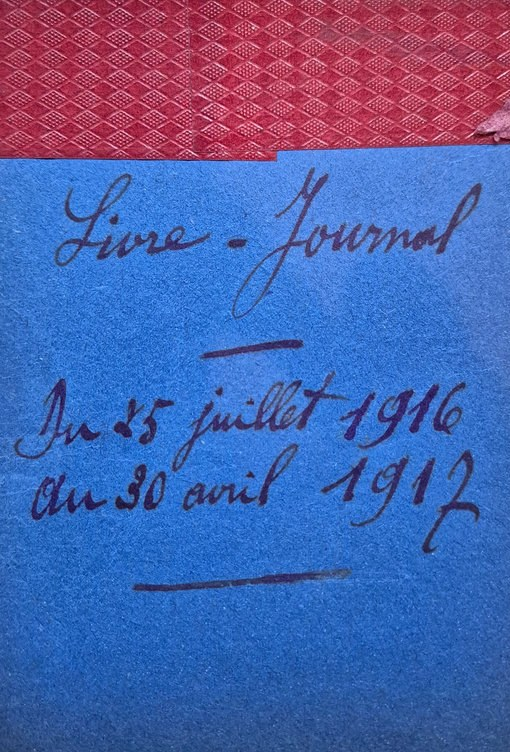
\includegraphics[width=58mm,height=50mm,keepaspectratio]{illustrations/vignette_couverture.jpg}%
        }\\[4.5mm]
        {\normalsize\textsc{Édition philologique, diplomatique et critique en vis-à-vis}}\\[2mm]
        {\scriptsize Transcription de travail des 186 vues, numérotée de 5 en 5 lignes,\\
        apparat critique marginal aligné dans le prolongement de la ligne,\\
        double registre de commentaire et fac-similés en regard}\par
        \vfill
        \rule{70mm}{0.4pt}\\[2mm]
        {\footnotesize\textsc{Édition établie, introduite et annotée}}\\
        {\scriptsize d'après le manuscrit autographe et les archives familiales Combes-Calmels de Millau et Montauban}\\[1.5mm]
        {\footnotesize\textbf{MMXXVI}}
        \vspace{1mm}
      \end{center}
    }%
  }
\end{center}
\end{titlepage}

% Page blanche de garde (Page 2)
\hbox{}\thispagestyle{empty}\newpage

% =============================================================================
% 2. FAUX-TITRE & PAGE DE TITRE INTÉRIEURE (AVEC EMBLÈME FRAKTUR \mathfrak{Urtext})
% =============================================================================
\thispagestyle{empty}
\begin{center}
  \vspace*{10mm}
  {\large\textsc{Marie Lucien Hippolyte Combes}}\\
  {\footnotesize (Millau, 14 août 1876 — Saint-Chély-d'Apcher, 2 septembre 1970)}\\[10mm]
  {\LARGE\textbf{LIVRE-JOURNAL DE GUERRE}}\\[3mm]
  {\normalsize\textit{25 juillet 1916 — 30 avril 1917}}\\[4mm]
  {\footnotesize Des Flandres à l'Artois et au front de la Somme\\
  auprès de l'\textit{Army Service Corps} (18\textsuperscript{e} Division, XIII\textsuperscript{e} \& V\textsuperscript{e} Corps)}\\[14mm]
  {\Huge $\mathfrak{Urtext}$}\\[14mm]
  \rule{45mm}{0.4pt}\\[6mm]
  {\footnotesize\textbf{Édition de travail : première collation des 186 vues}}\\[1.5mm]
  {\scriptsize accompagnée des lettres de guerre inédites (1916–1918), de l'état signalétique des services\\
  et d'un répertoire prosopographique, militaire et topographique}\par
  \vfill
  {\footnotesize\textsc{Collection des Sources et Manuscrits Contemporains}}\\
  {\scriptsize Millau — Toulouse — Montauban — Paris}
  \vspace*{6mm}
\end{center}
\newpage

\frontmatter
\renewcommand{\thesection}{\Roman{section}}
{\small\tableofcontents}
\cleardoublepage

% =============================================================================
% 3. PROLÉGOMÈNES SCIENTIFIQUES ET HISTORIQUES
% =============================================================================
\chapter{Prolégomènes : Hippolyte Combes (1876–1970) et son \textit{Livre-Journal} de la Grande Guerre}
\markboth{Prolégomènes}{Prolégomènes}
{\small

\section{Destin d'un universitaire rouergat et toulousain auprès de l'Armée britannique (1876–1970)}

L'acte de naissance n\textsuperscript{o}~395 du 16 août 1876 situe la naissance de \textbf{Marie Lucien Hippolyte Combes} à \textbf{Millau}, rue des Barris, le \textbf{14 août 1876}, fils de \textbf{François Augustin Hippolyte Combes} (1825–1899), avocat, et de \textbf{Marie Anaïs Alric} (1838–1907). La fiche matricule porte une date différente, le 22 août : les deux témoignages sont signalés sans harmonisation silencieuse. Les pièces d'état civil et monographies familiales (\texttt{Combes-3-part 1.DOC}, \texttt{Combes-3-part 2.DOC}, \texttt{Combes-annexe.DOC}) retracent ses études à l'Institution Sainte-Marie et à la Faculté des lettres de Toulouse (47 rue du Taur), son séjour de quatre années en Angleterre (Nottingham) et sa carrière de professeur d'anglais aux collèges de Saint-Yrieix et de Nogent-le-Rotrou (17 rue Saint-Hilaire), puis au lycée Ingres de Montauban jusqu'à sa retraite à Millau et son décès le \textbf{2 septembre 1970} à l'\textbf{Hôtel du Centre} à \textbf{Saint-Chély-d'Apcher} (Lozère ; date et commune dans \texttt{Combes-3-part 2.DOC}, établissement transmis par la tradition familiale directe ; inhumé à Millau).

\begin{figure}[htbp]
  \centering
  \begin{minipage}[b]{0.46\textwidth}
    \centering
    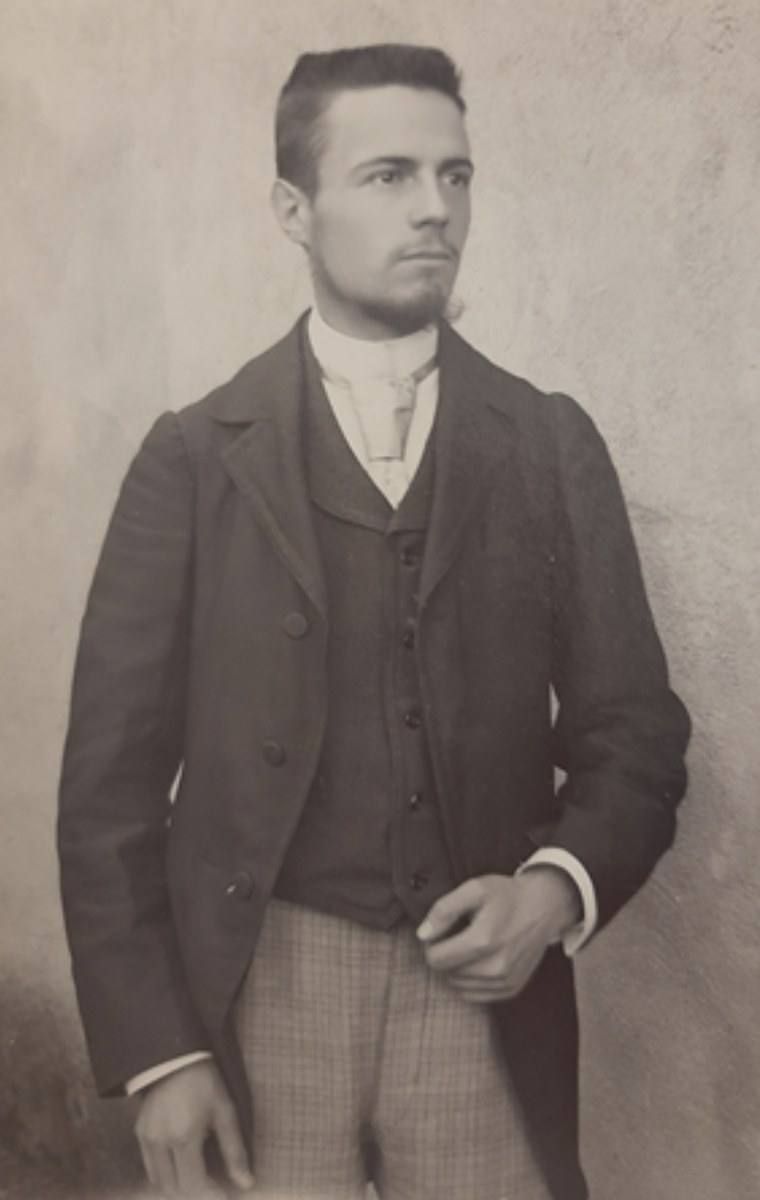
\includegraphics[height=44mm,keepaspectratio]{illustrations/hippolyte_1897.jpg}
    \par\vspace{1mm}{\scriptsize\textit{Fig. 1.} Hippolyte Combes en 1897, à l'âge de 21 ans.}
  \end{minipage}\hfill
  \begin{minipage}[b]{0.48\textwidth}
    \centering
    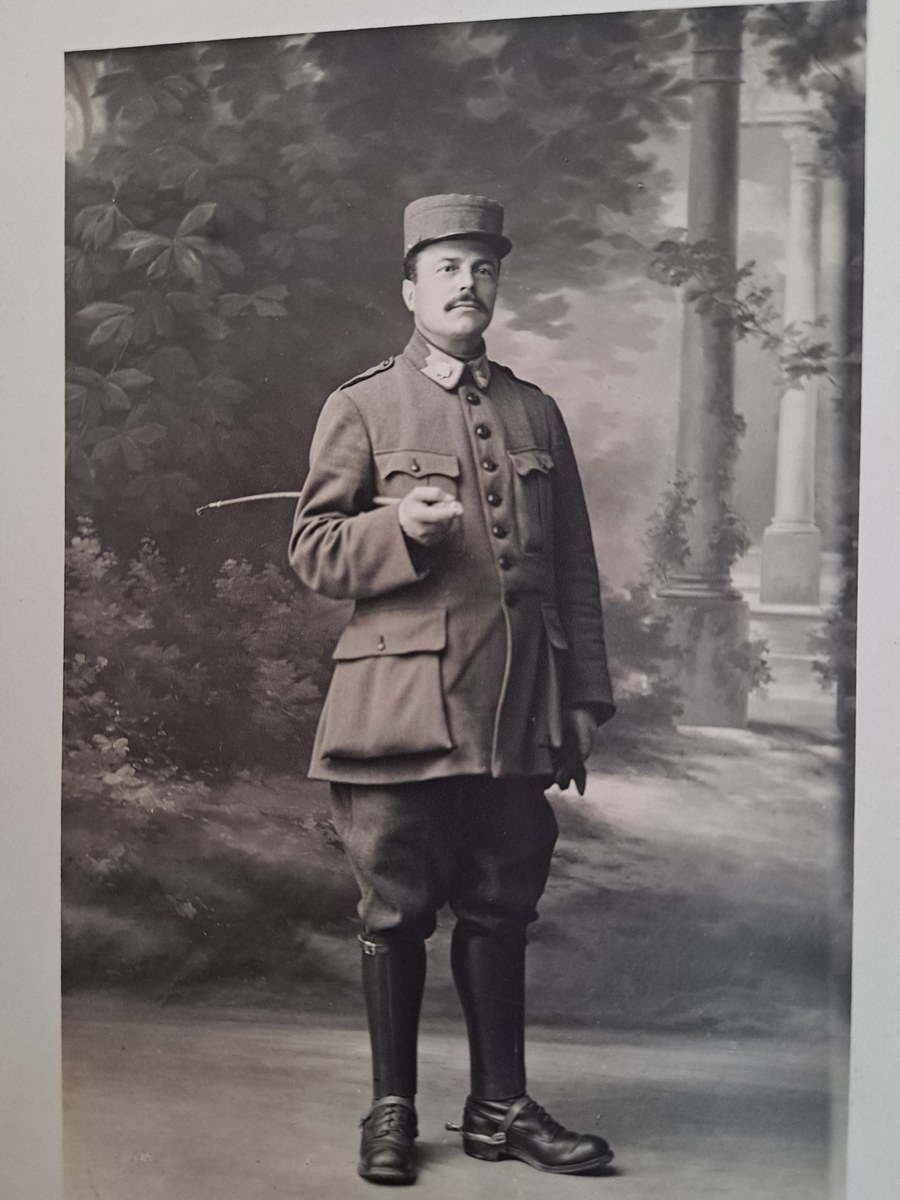
\includegraphics[height=44mm,keepaspectratio]{illustrations/hippolyte_interprete_1.jpg}
    \par\vspace{1mm}{\scriptsize\textit{Fig. 2.} Hippolyte Combes en uniforme d'interprète auprès de la B.E.F. (1916).}
  \end{minipage}
\end{figure}

Exempté dans sa jeunesse pour « faiblesse générale » (\textbf{classe 1896, bureau de recrutement de Toulouse, matricule n\textsuperscript{o}~911}), Hippolyte Combes est classé « Service armé » par le conseil de révision d'Eure-et-Loir le \textbf{18 décembre 1914}. Appelé à l'activité le \textbf{20 mars 1915} et incorporé le \textbf{21 mars 1915} à la 39\textsuperscript{e} batterie du \textbf{10\textsuperscript{e} régiment d'artillerie à pied} à Toulon (Saint-Jean-du-Var), il est détaché dès le \textbf{4 mai 1915} comme interprète militaire à la \textbf{Mission militaire française attachée à l'Armée britannique} (administrativement rattaché au \textbf{19\textsuperscript{e} escadron du Train des équipages militaires} le 15 octobre 1915) :

\begin{itemize}
  \item \textbf{Depuis août 1915 : service dans une compagnie A.S.C. de la 18\textsuperscript{e} Division britannique.} Dans la copie autographe de sa lettre du 21 février 1916 (Annexe I, document 1), Combes écrit avoir été rattaché à l'été 1915 à la \textbf{18\textsuperscript{e} Division britannique} (\textit{18th Eastern Division}, commandée par le major-général Sir Ivor Maxse) qui se formait autour de Flesselles, avoir servi quinze jours au secrétariat de la Mission française (sous l'officier interprète divisionnaire M.~Pizzi), puis être affecté « depuis le mois d'août » [1915] à une compagnie d'\textit{Army Service Corps}. Le carnet nomme la \textbf{152nd Company A.S.C.} et la \textit{54th Brigade} (vue \#066), situe une démarche au \textit{Train Office} auprès du \texttt{Col. Grose} (vue \#090), et signale le 9 janvier 1917 une visite à la \textbf{150th Company A.S.C., 18th Division}, près d'Hédauville (vue \#121). Ce dernier passage n'établit pas une affectation de trois jours à cette compagnie.
  \item \textbf{Du Train divisionnaire aux services d'achats et de réquisitions (\textit{Foraging} / \textit{Army Purchase Board}, juillet 1916 – avril 1917).} Le carnet suit d'abord les déplacements de Combes en Flandre intérieure (Sercus, Renescure, Hazebrouck, Bailleul) et dans la vallée de la Lys (La Croix-du-Bac, Armentières, Fleurbaix), puis son transfert ferroviaire du \textbf{25 août} vers Marquay par Saint-Pol (vues \#027–\#028) et sa remontée vers la Somme (Beauval, Raincheval, Acheux, Forceville). L'historique divisionnaire situe ces étapes après la relève de la Somme du 20 juillet 1916 et avant Thiepval (26 septembre) et les combats de l'Ancre. À Acheux-en-Amiénois, puis à Hérissart, Combes décrit le service des approvisionnements et achats de fourrage, d'abord avec le capitaine Williams. Le 11 mars, il apprend son maintien au \textit{Purchase Board} sur demande du major Levy (vue \#166) ; il fréquente ensuite notamment le lieutenant Gilbert, donné comme originaire de Jersey (vue \#179).
  \item \textbf{Après le carnet.} Les pièces familiales documentent son mariage avec \textbf{Marie Marguerite Calmels} (1892–1974) à Millau le 25 octobre 1917. La fiche matricule donne son affectation à l'École militaire préparatoire des Andelys comme professeur d'anglais le 24 novembre 1918 (nommé caporal le 4 décembre 1918) et sa démobilisation le 7 février 1919. La mention de Montauban du 24 janvier 1920 relève de la rubrique des domiciles et indique sa profession au lycée Ingres.
\end{itemize}

\section{Histoire matérielle, codicologie et paléographie du \textit{Livre-Journal}}

Le dossier photographique comprend \textbf{186 clichés numériques}, de \texttt{20251126\_\allowbreak 092853.jpg} (Scan \#001) à \texttt{20251126\_\allowbreak 111833.jpg} (Scan \#186). Le premier cliché reproduit le plat supérieur de la couverture, revêtu d'un papier fort rouge à motif de losanges gaufrés sur lequel est collée une étiquette rectangulaire de papier bleu portant à l'encre noire l'intitulé autographe en cinq lignes : \textit{Livre - Journal / — / Du 25 juillet 1916 / au 30 avril 1917 / —}.

Cette édition de travail résulte d'une première collation, puis d'une étude comparative de l'écriture suivie d'une seconde relecture intégrale des 186 vues. Un atlas de 88 extraits natifs, issus de 54 photographies, documente les comparaisons dans le dépôt ; cette seconde passe modifie les lignes transcrites de 49 vues. Elle conserve les doutes de lecture. Les observations ci-dessous décrivent des usages fréquents ; elles ne remplacent pas la vérification de chaque tracé.
\begin{enumerate}
  \item \textbf{Ductus et système abréviatif d'Hippolyte Combes.} L'écriture d'Hippolyte Combes est une cursive latine penchée, rapide et nerveuse, riche en abréviations par suspension et par lettres suscrites : \textit{ds} (\textit{dans}), \textit{pr} (\textit{pour} ou \textit{par}, selon la phrase), \textit{s/} (\textit{sur}), \textit{j'à / j'au / j'aux} ou \textit{ju} (\textit{jusqu'à, jusqu'au, jusqu'aux}), \textit{lgt / lgs / longt} (\textit{longtemps}), \textit{tt / tte / ts} (\textit{tout, toute, tous}), \textit{tjs / tjours} (\textit{toujours}), \textit{qq} (\textit{quelque} ou \textit{quelques}, selon la phrase), \textit{gd / gde / gds} (\textit{grand, grande, grands}), \textit{bp / bcp} (\textit{beaucoup}), \textit{cme} (\textit{comme}), \textit{chz} (\textit{chez}), ainsi que les finales adverbiales ou nominales suscrites (\textit{ext\textsuperscript{t}, merv\textsuperscript{t}, défin\textsuperscript{t}, admirab\textsuperscript{t}, appart\textsuperscript{t}, cantonnem\textsuperscript{t}, changem\textsuperscript{t}, propri\textsuperscript{re}, cath\textsuperscript{le}}). Les chiffres peuvent avoir une valeur lexicale : 1 pour un ou une, 1/2 pour demi ou, selon le contexte, milieu. Les signes $+$ et $=$ sont conservés ; leur développement est motivé dans la notice, et non imposé partout.
  \item \textbf{Esperluette et y.} Certains tracés cursifs de \texttt{\&} ressemblent à la lettre y. Leur valeur est examinée occurrence par occurrence, d'après la forme, la position et les parallèles de la main. Aucun remplacement global de y par et ou par \texttt{\&} n'est appliqué comme règle de lecture ; un signe non établi reste marqué.
  \item \textbf{Lectures et identifications vérifiées.} Curtis est lisible dans plusieurs entrées et apparaît aussi sous la contraction \textit{Ctis}. La vue \#016 porte la date du 10 août, mentionne Sailly-sur-la-Lys et rapporte une conversation avec un éclusier au sujet du général Maxse. À la vue \#142 (l.~6, Millau, 4 février 1917), la réinspection du cliché établit \texttt{visite à l'oncle \& tante Thérèse (Layral)}. L'annexe familiale identifie Thérèse Cartairade et son époux Charles Layrals, notaire à Millau, avec un s final dans cette source. Spagnol est cité ailleurs, à propos d'un télégramme à Nice et d'un règlement (vues \#136 et \#158) ; le métier de fleuriste demeure conjectural. Le rapprochement des Flutre de la vue \#168 avec la famille du romaniste Louis-Fernand Flutre repose sur la nécrologie de René Debrie (1978, p.~238--240), qui nomme son père Fortuné, instituteur au Mesnil-Martinsart. Debrie donne une naissance au Mesnil-Martinsart, tandis que la BnF (\texttt{cb122063529}) indique Albert ; cette divergence n'est pas expliquée par les documents consultés. Debrie distingue l'admission à l'ENS en 1914, l'entrée en 1919 et l'agrégation en 1921. Le second prénom Ernest, la naissance du père en 1862 et son installation en 1888 demandent encore une pièce directement contrôlable.
  \item \textbf{Particularités de la séquence photographique.} Le cliché \#050 (\texttt{20251126\_\allowbreak 103019.jpg}, journée du 25 septembre 1916), omis dans le premier fichier Word, est restitué à sa place. Les clichés \#063 (5 octobre 1916) et \#064 (nuit du 4 au 5 octobre 1916), ainsi que les clichés \#112 (22 et 24 décembre 1916) et \#113 (19 et 20 décembre 1916), ont été photographiés dans l'ordre inverse de la chronologie. Enfin, les clichés \#091 (\texttt{20251126\_\allowbreak 104623.jpg}) et \#093 (\texttt{20251126\_\allowbreak 104648.jpg}) constituent deux prises de vue successives d'un même feuillet original (journées des 2 et 3 novembre 1916). Pour conserver une correspondance explicite avec les 186 fichiers JPEG des répertoires \texttt{scans\_\allowbreak haute\_\allowbreak qualite/} et \texttt{scans\_\allowbreak compresses/}, l'édition conserve la numérotation des vues (\texttt{Scan \#001} à \texttt{Scan \#186}). La désignation Vue identifie une photographie ; elle ne constitue pas une foliation matérielle. Les anciens numéros recto-verso calculés d'après l'ordre des fichiers n'ont pas valeur de constat codicologique.
\end{enumerate}

\section{Principes de l'édition philologique en vis-à-vis}

Inspirée des principes de l'édition philologique classique (sur le modèle de l'édition savante des \textit{Thesmophories} d'Aristophane), la présente édition adopte un format agrandi (\texttt{185 $\times$ 270 mm}, de proportions proches du carnet photographié), pour conserver l’apparat complet sur la page en regard du cliché, une typographie sobre en noir sur fond blanc pur et met en regard, sur chaque double page (du Scan \#001 au Scan \#186) :
\begin{itemize}
  \item \textbf{Sur la page de gauche (page paire / verso) :}
    \begin{enumerate}
      \item \textbf{La transcription de travail ligne à ligne}, cherchant à conserver l'orthographe, les abréviations et la ponctuation. Les lignes sont numérotées de cinq en cinq dans la marge gauche (\texttt{5, 10, 15, 20, 25}). Les crochets simples \texttt{[ ... ]} peuvent signaler une réserve éditoriale ou isoler un compte : leur présence dans la transcription ne prouve pas un crochet autographe ni une écriture en marge ; la disposition réellement observée est décrite dans l'apparat. Les lectures proposées portent un point d'interrogation ; \texttt{[illis.]} signale une séquence écrite non déchiffrée, sans impliquer une lacune matérielle. Les blancs, ajouts et suppressions sont signalés d'après la photographie ; les ratures autographes lisibles sont placées entre doubles crochets droits ($[\![ \dots ]\!]$). Aucun soulignement, exposant ou trait autographe n'est déduit d'une règle de remplacement appliquée au seul texte.
      \item \textbf{L'apparat critique marginal}, entièrement repris à partir des photographies, est ancré sur un numéro de ligne et un lemme exact en gras. Les développements d'abréviation sont en italique, fléchis et expliqués selon la phrase ; les emprunts anglais (\textit{angl.}), latins (\textit{lat.}) ou hybrides (\textit{hybr.}) sont traduits selon leur emploi. Les ratures, ajouts, signes, réserves et particularités de disposition sont décrits explicitement. Toutes les entrées retenues sont rendues, sans plafond par ligne ni fusion entre lignes distinctes. Une ellipse syntaxique n'est pas traitée comme une abréviation ; une identité ou un développement conjectural reste donné comme tel.
      \item \textbf{Unités et signes usuels.} \textit{etc.} abrège \textit{et cetera}. Dans les comptes, \textit{f} et \textit{fr} désignent les francs, \textit{c} les centimes ; dans les heures, \textit{h} ou \textit{H} désignent l'heure, \textit{m} le matin ou les minutes selon la notation, \textit{s} le soir. Les fractions horaires ordinaires se lisent sans développement local répétitif. L'esperluette \texttt{\&} vaut et ; le signe $+$ vaut plus ou une addition selon la phrase ou le compte. Le signe $=$ conserve sa valeur contextuelle : égalité comptable, reprise ou abréviation de même selon les occurrences. Une note locale précise les emplois ambigus, notamment \textit{1/2 jour} (milieu du jour), et les quantités dont l'unité n'est pas écrite. Ces conventions ne permettent pas d'attribuer à un montant une unité ou une opération absente du manuscrit.
      \item \textbf{En bas de page, deux registres de commentaires dépourvus d'intitulés répétitifs mais immédiatement distingués au premier coup d'œil par des filets horizontaux et un décrochement typographique franc :}
        \begin{itemize}
          \item \textit{Le premier registre}, placé immédiatement sous le filet horizontal de pleine largeur (\texttt{0,5 pt}) et composé au fer à gauche sur toute la justification (\texttt{163 mm}), est consacré à la \textbf{critique interne du carnet} : analyse codicologique et paléographique, génétique des repentirs, syntaxe elliptique, bilinguisme franco-anglais, tenue des comptes et degrés de certitude des lectures.
          \item \textit{Le second registre}, séparé du précédent par un filet horizontal court (\texttt{38 mm}, \texttt{0,4 pt}) et composé avec un retrait général de bloc de \texttt{5 mm} sur la gauche, est consacré à l'\textbf{élucidation historique, militaire, topographique et prosopographique} : références militaires et géographiques, localités et personnes mentionnées, avec distinction entre lecture, hypothèse d'identification et fait établi par une source extérieure.
        \end{itemize}
    \end{enumerate}
  \item \textbf{Sur la page de droite (page impaire / recto) :} \textbf{le fac-similé photographique complet} du feuillet manuscrit correspondant, accompagné de ses références archivistiques.
\end{itemize}

\section{Critique des sources militaires et archivistiques}

L'annotation historique repose sur le croisement méthodique des archives familiales du dépôt (\texttt{archives\_\allowbreak militaires/} et \texttt{biographie\_\allowbreak et\_\allowbreak famille/}) et des sources institutionnelles britanniques et françaises :
\begin{itemize}
  \item \textbf{18th (Eastern) Division et 18th Divisional Train A.S.C.} L'historique divisionnaire du capitaine G.~H.~F.~Nichols (\textit{The 18th Division in the Great War}, Londres, Blackwood, 1922, p.~107--110 et 432) et l'\textit{Order of Battle of Divisions} du major A.~F.~Becke (Part~3A, Londres, HMSO, 1938) établissent que le \textit{18th Divisional Train} comprenait quatre compagnies d'\textit{Army Service Corps} (\textbf{150th, 151st, 152nd et 153rd Companies A.S.C.}), commandées à Thiepval par le \textbf{Lt.-Col. D.~C.~E.~Grose, A.S.C.} (\textit{London Gazette}, 4 juin 1917, p.~5470 ; \texttt{Col. Grose} au \textit{Train Office}, vue \#090), avec notamment le \textbf{Maj. H.~G.~Peachy, A.S.C.} à la \textbf{150th Co.} et le \textbf{Capt. E.~M.~West, A.S.C.} à la \textbf{152nd Co.} (\textit{Military Cross}, p.~432 ; \texttt{Cap. West}, vues \#039, \#042, \#048), ainsi que le \textbf{Capt. E.~M.~Ford, M.C.} au \textit{18th Div. Train} (p.~432 ; \texttt{Lt Ford}, vue \#076). \textit{The Ringing World} (9 avril 1915, p.~184) atteste dès 1915 la \textbf{152nd Company A.S.C.} au \textit{18th Divisional Train}. Combes indique la \textbf{152nd Company A.S.C.} et la \textit{54th Brigade} (vue \#066), puis la \textbf{150th Company A.S.C., 18th Division} (vue \#121, 9 janvier). Il nomme des \textit{Royal Fusiliers} (vues \#002–\#003) et des \textit{Bedfords} (vue \#038), sans numéro de bataillon dans ces mentions. La vue \#150 porte \textit{M.T. (A.S.C.)}, à développer comme \textit{Motor Transport} ; la notice de la \textit{London Gazette} du 9 mars 1917, p.~2447, ne suffit pas à identifier l'unité personnelle de Combes à cette date.
  \item \textbf{Grandes unités alliées croisées dans la Somme en 1917.} La vue \#164 rattache l'interprète Valet à la \textbf{2nd Australian Division} ; elle ne décrit pas à elle seule la relève de tout le secteur. Combes observe des cavaliers indiens et anglais et nomme les \textbf{17th Lancers (\textit{Death or Glory Boys})} à la vue \#171. L'historique du Royal Lancers Museum rattache ce régiment à la \textit{1st Indian Cavalry Division} lors de son arrivée en France en 1914 ; le rattachement précis de tous les cavaliers aperçus aux vues \#160, \#169 et \#171 ne peut être déduit de leur seule présence. Aux vues \#170–\#171, Combes loge un officier de la \textbf{63rd Division, naval division}, dont le régiment revient des tranchées de Miraumont et d'Achiet-le-Petit. Ces mentions éclairent le repli allemand de mars 1917, sans établir que toutes les brigades de cette division reviennent ensemble des deux localités.
\end{itemize}

\section{Répertoire prosopographique, militaire et topographique}

{\footnotesize
\renewcommand{\arraystretch}{1.15}
\noindent\begin{longtable}{@{}>{\raggedright\arraybackslash}p{33mm}p{95mm}@{}}
\toprule
\textbf{Nom / Unité / Lieu} & \textbf{Identification biographique, militaire ou géographique} \\
\midrule
\endhead
\textbf{Combes, Hippolyte} (1876–1970) & Marie Lucien Hippolyte Combes, né à Millau le 14 août 1876 (acte n\textsuperscript{o}~395 ; 22 août sur la fiche matricule), décédé le 2 septembre 1970 à l'Hôtel du Centre à Saint-Chély-d'Apcher (Lozère ; date et commune dans \texttt{Combes-3-part 2.DOC}, établissement transmis par la tradition familiale directe ; inhumé à Millau). Professeur d'anglais à Saint-Yrieix, Nogent-le-Rotrou (17 rue Saint-Hilaire) puis au lycée Ingres de Montauban ; interprète militaire auprès de l'Armée britannique (4 mai 1915 – 11 novembre 1918). \\
\textbf{Calmels, Marguerite} (« Margte », « Mte », « Gueïte », 1892–1974) & Marie Marguerite Calmels, née à Millau le 15 avril 1892 (acte n\textsuperscript{o}~139, \texttt{1892\_acte\_naissance\_Marguerite\_Calmels.png}) et décédée à Millau le 19 mars 1974 (\texttt{biographie\_et\_famille/etat\_civil\_et\_actes/}), fille du Dr Gabriel Calmels (1852–1921) et de Valentine Cartairade (1858–1943), domiciliés au 10 rue Alfred-Guibert à Millau. Fiancée puis épouse d'Hippolyte Combes (25 octobre 1917). \\
\textbf{Combes, François-Hippolyte} (1825–1899) \& \textbf{Marie Anaïs Alric} (1838–1907) & Parents d'Hippolyte Combes : François Augustin Hippolyte Combes, avocat à Millau puis installé à Toulouse (47 rue du Taur), et Marie Anaïs Alric (Scans \#092, \#132, \#143). \\
\textbf{Françoise} (1871–1942), \textbf{Joséphine} (1873–1914) \& \textbf{Maria} (1875–1903) & Les trois sœurs d'Hippolyte Combes : Françoise (\textit{Sœur Marie de la Croix}, carmélite à Périgueux, destinataire de la lettre du 16 juin 1916), Joséphine (décédée chez Hippolyte à Nogent-le-Rotrou en octobre 1914) et Maria (religieuse décédée à Carthage le 19 novembre 1903). \\
\textbf{Crouzet, Émile} (1842–1921), \textbf{Élisabeth Calmels} \& \textbf{l'abbé Jean Crouzet} & Famille toulousaine chez qui réside Marguerite lors des permissions de septembre 1916 et janvier 1917 (47 rue du Taur et rue Pharaon) : Émile Crouzet (\texttt{M. Czt}, \texttt{oncle Crouzet}, \texttt{Oncle Émile}, agent de change à Toulouse, témoin de 39 ans sur l'acte de naissance n\textsuperscript{o}~139 de Marguerite en 1892), son épouse Élisabeth Calmels (\texttt{Tante}, tante paternelle de Marguerite) et leur fils l'abbé Jean Crouzet (\texttt{Jean}, prêtre, futur curé de Notre-Dame de la Dalbade ; \texttt{Combes-annexe.DOC}). \\
\textbf{Calmels, Vincens et Delcamps (familles)} & Famille de Marguerite au 10 rue Alfred-Guibert à Millau (Scans \#139–\#143) : le Dr Gabriel Calmels (1852–1921) et Valentine Cartairade (1858–1943) ; leurs filles Madeleine Calmels (1882–1961, épouse du Dr Fernand Vincens, mère de \textbf{Germaine} et \textbf{Robert Vincens}), Anne-Marie dite \textbf{« Mimi »} Calmels (1888–1975, future épouse de l'avoué Joseph Delcamps) et Marguerite, ainsi que leur fils \textbf{Pierre Calmels}. \\
\textbf{Layral, M\textsuperscript{e} Charles \& Thérèse Cartairade} & Oncle et tante maternels de Marguerite à Millau, visités le 4 février 1917 : \texttt{visite à l'oncle \& tante Thérèse (Layral)} (Scan \#142, l.~6 ; \texttt{Combes-annexe.DOC} et \texttt{faire-part-deces-Emilie-Noel.jpg}). \\
\textbf{Faure, Mme} (Germaine, Marcel, Henri, André) & Famille reçue à Neuilly-sur-Seine (vues \#130–\#131) ; la lecture du premier chiffre de l'adresse demeure réservée ; l'annexe familiale réserve expressément le degré de parenté. Marcel est présent lors de la visite de janvier 1917 (vue \#131). L'identification au futur Compagnon de la Libération Marcel Faure est proposée par la notice familiale et demande une vérification indépendante. Le récit de captivité et de rapatriement que l'ancienne annexe attribuait aux lettres des 25 et 26 novembre 1918 ne figure pas dans les quatre faces écrites contrôlées : ces pièces relatent la visite chez les Faure et des conversations familiales. \textbf{Henri} est dit aspirant et \textbf{André} prépare Polytechnique. \\
\textbf{Chilcott, Beatrice} & Amie anglaise d'Hippolyte Combes à l'époque de son séjour d'avant-guerre à Nottingham, signataire du poème autographe conservé dans ses papiers (\textit{Wesley Band of Hope}). \\
\textbf{Maxse, Maj.-Gen. Sir Ivor} (1862–1958) & Commandant de la \textbf{18th (Eastern) Division} britannique de 1915 à janvier 1917. Combes parle de lui avec un éclusier le 10 août 1916 lors de sa promenade vers Sailly-sur-la-Lys (vue \#016) ; aucune rencontre avec le général n'est rapportée dans ce passage. \\
\textbf{Grose, Lt.-Col. Daniel Charles Evans} & Commandant (\textit{Officer Commanding}) du \textbf{18th Divisional Train, A.S.C.} (DSO, \textit{London Gazette}, 4 juin 1917, p.~5470 ; Nichols, 1922, p.~110), mentionné au Scan \#090 (\texttt{Col. Grose}). \\
\textbf{152nd \& 150th Companies, A.S.C.} & Compagnies du \textbf{18th Divisional Train} (\textbf{150th, 151st, 152nd et 153rd Companies A.S.C.}, Nichols, 1922, p.~107--110 ; \textit{The Ringing World}, 9 avril 1915, p.~184). Combes nomme la \textbf{152nd Company} et la \textit{54th Brigade} à la vue \#066, puis visite la \textbf{150th Company, 18th Division} près d'Hédauville le 9 janvier 1917 (vue \#121). Les mentions de \textit{Royal Fusiliers} et de \textit{Bedfords} ne donnent pas à elles seules les numéros de bataillon. \\
\textbf{Curtis} (\textit{Ctis}), \textbf{Panton}, \textbf{West}, \textbf{Walsh}, \textbf{Ford} & Officiers britanniques mentionnés par Combes de juillet à novembre 1916. Nichols (1922, p.~110, 432) atteste au \textbf{18th Divisional Train} le \textbf{Capt. E.~M.~West, A.S.C.} (commandant la \textbf{152nd Co. A.S.C.} à Thiepval, décoré de la \textit{Military Cross}) et le \textbf{Capt. E.~M.~Ford, M.C.} ; l'unité exacte de Curtis, Panton et Walsh n'est pas précisée par le carnet. \\
\textbf{Williams, Capt.} & Capitaine britannique (\textit{Foraging Officer}) avec qui Combes effectue les tournées de réquisition de paille et de fourrage autour d'Acheux et d'Hérissart du 1\textsuperscript{er} décembre 1916 au 10 mars 1917 (Scans \#105–\#165). \\
\textbf{Levy, Major} \& \textbf{Gilbert} & Le major Levy demande le maintien de Combes au \textit{Purchase Board}, ce qu'il apprend le 11 mars 1917 (vue \#166). Le \textit{Second Lieutenant} Gilbert est dit originaire de \textbf{Jersey}, instruit et poète (vue \#179) ; Combes décrit ensuite leurs conversations et promenades. Ces mentions ne suffisent pas à établir une succession formelle au poste du capitaine Williams. \\
\textbf{Pizzi, Ferran, Huguet, Raucoule, Valet} & Officiers et interprètes rencontrés ou mentionnés dans le dossier de la Mission française. Leurs rattachements doivent être établis séparément ; le petit numéro interlinéaire de la vue \#094 demeure réservé. \\
\textbf{Flutre, Fortuné} \& \textbf{Louis-Fernand Flutre} (1892–1978) & Le couple d'instituteurs rencontré au Mesnil et leur fils normalien (vue \#168) se rapprochent fortement de cette famille : René Debrie (nécrologie, 1978, p.~238--240) nomme Fortuné, instituteur au \textbf{Mesnil-Martinsart}, comme père du romaniste. Il situe la naissance du fils dans ce village le 21 juin 1892 ; la notice BnF \texttt{cb122063529} indique \textbf{Albert}. Louis-Fernand est admis à l'ENS en \textbf{1914}, y entre en \textbf{1919}, est agrégé en \textbf{1921}, puis enseigne la philologie romane à Lyon ; il publie deux monographies de son village en 1955. Le second prénom Ernest et les dates du père restent à vérifier directement. \\
\textbf{Zyromski, Ernest} (1862–1933) & Professeur de littérature française à la Faculté des lettres de Toulouse ; Hippolyte achète son essai \textit{L'Orgueil humain} chez Armand Colin le 26 septembre 1916 (Scan \#053) et assiste à sa conférence sur Maurice de Guérin le 30 janvier 1917 (Scan \#135). \\
\textbf{Labit, Antoine} (1832–1912) \& \textbf{Georges} (1862–1899) & Père et fils : Antoine Labit est associé au grand magasin toulousain \textit{La Maison Universelle} et Georges fonde le musée portant son nom (INHA, notice Labit ; POP, \texttt{IA31110776}). Combes mentionne les magasins Labit à la vue \#134. Les vues \#057–\#058 n'établissent pas une visite au musée. \\
\bottomrule
\end{longtable}
}
\par}

\mainmatter
\renewcommand{\thesection}{\thechapter.\arabic{section}}

% =============================================================================
% CHAPITRE I (SCANS #001 A #018)
% =============================================================================
\cleardoublepage
\chapter{De la Flandre intérieure à la vallée de la Lys}
\markboth{Chapitre I — De la Flandre intérieure à la vallée de la Lys}{Scans \#001 à \#018}

\noindent{\fontsize{8pt}{9.2pt}\selectfont\textit{Renescure, Hazebrouck, Saint-Jans-Cappel, Bailleul et La Croix-du-Bac (25 juillet – 12 août 1916)}}\par\vspace{1.2mm}
\noindent\rule{\textwidth}{0.5pt}\par\vspace{0.7mm}
\noindent\textbf{\scriptsize\textsc{Argument analytique (Scans \#001 à \#018)}}\par\vspace{0.4mm}
\noindent{\fontsize{6.6pt}{7.6pt}\selectfont La couverture ouvre le dossier (vue \#001). Les entrées suivantes décrivent le cantonnement d'officiers à Sercus, les tournées de fourrage avec Curtis à Lynde, les visites de Renescure, Hazebrouck et Bailleul, puis l'installation au hameau de La Croix-du-Bac (Steenwerck) dans la vallée de la Lys. Le bombardement d'Armentières du 11 août et les biffures relatives à un soldat condamné demandent une lecture prudente (vue \#017).}\par\vspace{0.7mm}
\noindent\rule{\textwidth}{0.3pt}\par\vspace{1.2mm}

\noindent\textbf{\scriptsize\textsc{Introduction historique et philologique}}\par\vspace{0.5mm}
{\fontsize{7.1pt}{8.2pt}\selectfont Relevée de la Somme le 20 juillet 1916 après les combats du bois des Trônes, la \textit{18th (Eastern) Division} du major-général Sir Ivor Maxse gagne la Flandre intérieure avant de tenir le secteur de la Lys autour d'Armentières et de Fleurbaix (Capt. G. H. F. Nichols, \textit{The 18th Division in the Great War}, 1922, p. 81--85). Ce contexte divisionnaire éclaire les déplacements de Combes, détaché depuis août 1915 auprès d'une compagnie d'\textit{Army Service Corps} (lettre du 21 février 1916 ; \textit{152nd Company A.S.C.} et \textit{54th Brigade} à la vue \#066). Il mentionne les \textit{Royal Fusiliers} aux vues \#002--\#003, sans numéro de bataillon, décrit le clocher de Sercus (vue \#002), deux châteaux qu'il qualifie du Moyen Âge à Renescure (vue \#004) et l'architecture flamande de Bailleul (vues \#008--\#009). À la vue \#016, il parle du général Maxse avec un éclusier ; il ne rapporte pas de rencontre avec le général.}

\vfill
\noindent\begin{center}
  \begin{minipage}[b]{0.46\textwidth}
    \centering
    \setlength{\fboxsep}{0.7mm}\setlength{\fboxrule}{0.4pt}%
    \fcolorbox{gray!55}{white}{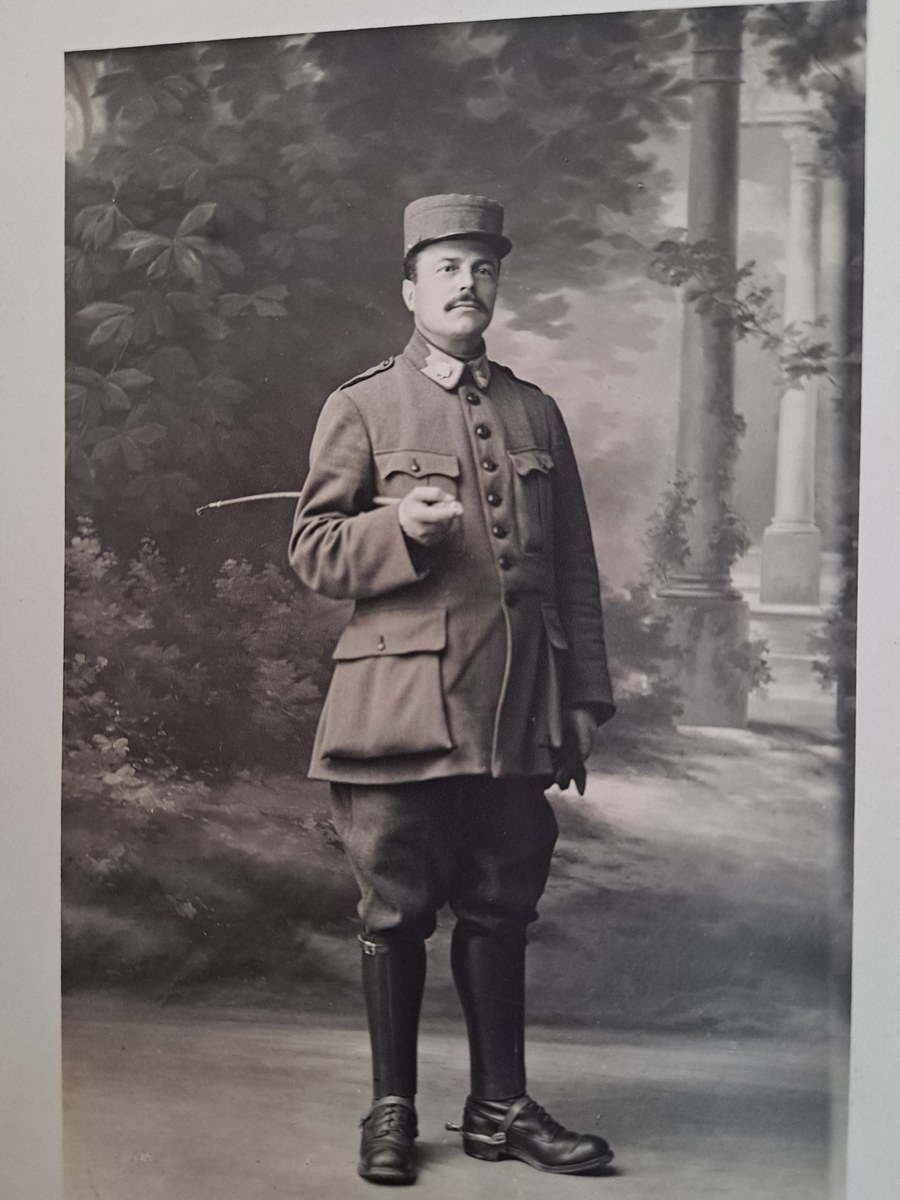
\includegraphics[width=0.94\linewidth,height=22mm,keepaspectratio]{illustrations/hippolyte_interprete_1.jpg}}
    \par\vspace{0.6mm}{\fontsize{5.8pt}{6.7pt}\selectfont Hippolyte Combes en uniforme d'interprète militaire attaché à l'Armée britannique (képi à bandeau et insignes de col au sphinx). Collection familiale Combes.}
  \end{minipage}\hfill
  \begin{minipage}[b]{0.46\textwidth}
    \centering
    \setlength{\fboxsep}{0.7mm}\setlength{\fboxrule}{0.4pt}%
    \fcolorbox{gray!55}{white}{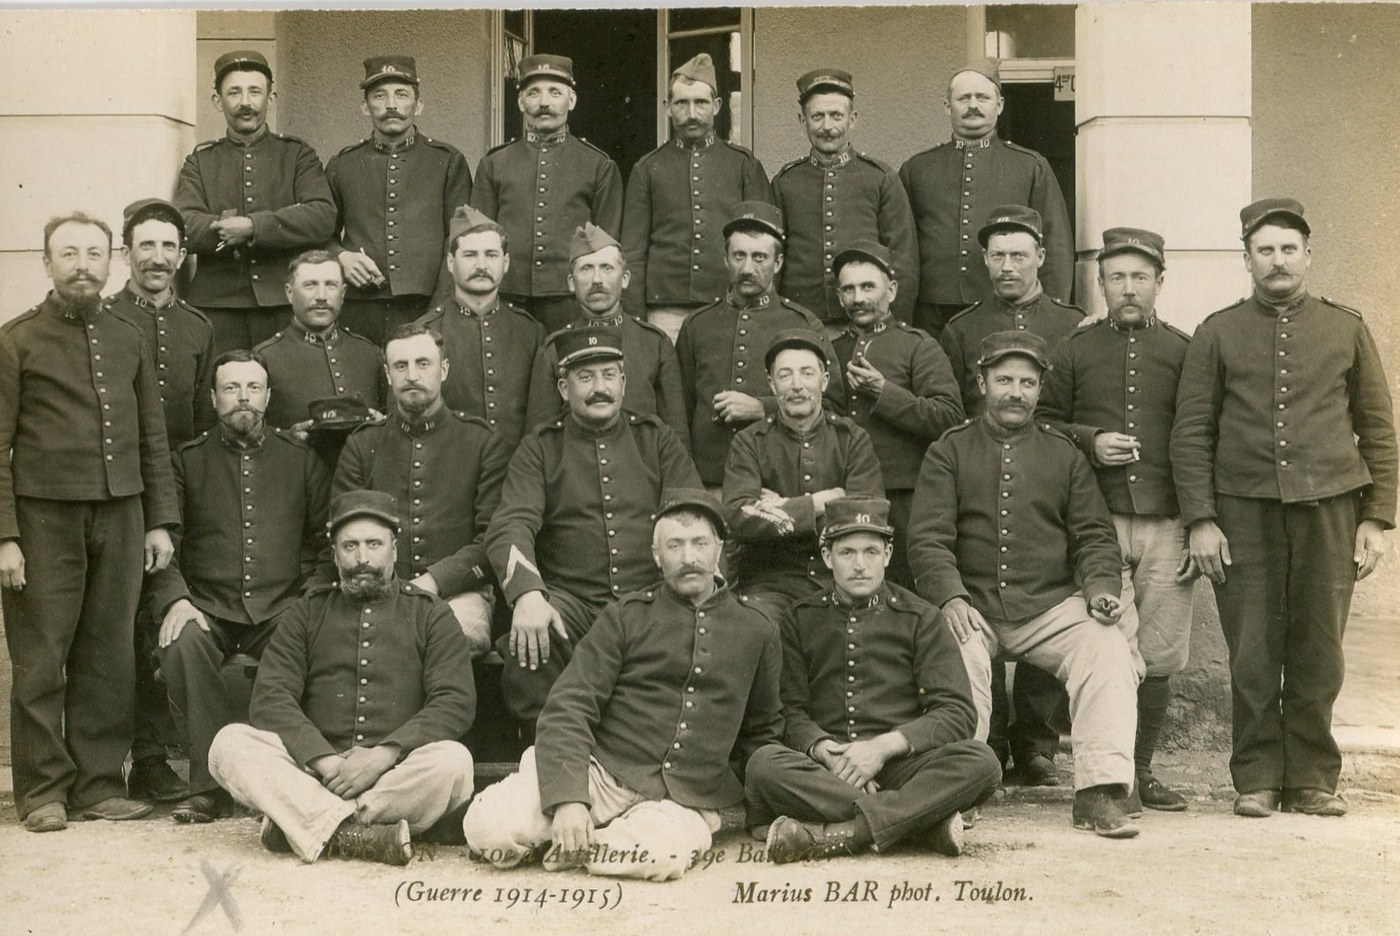
\includegraphics[width=0.94\linewidth,height=22mm,keepaspectratio]{illustrations/toulon_artillerie_1915.jpg}}
    \par\vspace{0.6mm}{\fontsize{5.8pt}{6.7pt}\selectfont Hippolyte Combes au 10\textsuperscript{e} régiment d'artillerie à pied à Toulon (Saint-Jean-du-Var) au printemps 1915.}
  \end{minipage}
\end{center}
\clearpage

% =============================================================================
% VIS-A-VIS SPREAD : SCAN #001 (20251126_092853.jpg) — Couverture extérieure
% =============================================================================
\cleardoubleevenpage
% --- En-tête du folio (Page paire / gauche : Transcription, apparat & double registre) ---
\noindent\rule{\textwidth}{0.5pt}\par\vspace{0.6mm}
\noindent\textbf{\footnotesize SCAN \#001 — COUVERTURE EXTÉRIEURE} \hfill {\scriptsize\texttt{20251126\_\allowbreak 092853.jpg}}\par\vspace{0.3mm}
\noindent{\fontsize{7.0pt}{8.2pt}\selectfont PREMIÈRE DE COUVERTURE (Couverture rouge à motif losangé et étiquette bleue rectangulaire : Livre-Journal, 25 juillet 1916 – 30 avril 1917)}\par\vspace{0.25mm}
\noindent{\fontsize{7.0pt}{8.2pt}\selectfont\textit{25 juillet 1916 – 30 avril 1917} \hfill \textit{Somme, Flandres, Artois, Paris, Toulouse, Millau}}\par\vspace{0.6mm}
\noindent\rule{\textwidth}{0.35pt}\par\vspace{1.0mm}
% --- Corps de la transcription diplomatique et apparat marginal en prolongement ---
{\renewcommand{\arraystretch}{1.02}%
\noindent\hspace*{3.5mm}\begin{tabular}{@{}p{100mm}@{\hspace{3.5mm}}p{55mm}@{}}
      \leavevmode\fontsize{7.8pt}{9.2pt}\selectfont\strut Livre - Journal\strut &  \\
      \leavevmode\fontsize{7.8pt}{9.2pt}\selectfont\strut —\strut &  \\
      \leavevmode\fontsize{7.8pt}{9.2pt}\selectfont\strut Du 25 juillet 1916\strut &  \\
      \leavevmode\fontsize{7.8pt}{9.2pt}\selectfont\strut au 30 avril 1917\strut &  \\
      \leavevmode\llap{\fontsize{6.5pt}{7.5pt}\selectfont\color{darkgray}5\hspace{1.8mm}}\fontsize{7.8pt}{9.2pt}\selectfont\strut —\strut &  \\
\end{tabular}}%
\par\vspace*{\fill}
% --- Deux registres de commentaires en bas de page (sans intitulés, distingués par filets et mise en page) ---
\noindent\rule{\textwidth}{0.5pt}\par\vspace{0.8mm}
{\fontsize{6.8pt}{8.0pt}\selectfont%
\noindent\normalfont Étiquette bleue sur couverture rouge à décor de losanges. Un trait sépare le titre des bornes chronologiques et un autre clôt l’inscription. Les cinq lignes ne présentent ni contraction à développer ni suppression visible ; les dates sont celles annoncées par le titre, sans date démontrée de sa rédaction.\par\vspace{0.75mm}
\noindent\rule{38mm}{0.4pt}\par\vspace{0.65mm}
\noindent\hspace*{5mm}\parbox{\dimexpr\textwidth-5mm\relax}{\fontsize{6.8pt}{8.0pt}\selectfont\color{black!82}Les dates de couverture bornent le carnet d’Hippolyte Combes (né à Millau le 14 août 1876, décédé le 2 septembre 1970 à l’Hôtel du Centre à Saint-Chély-d’Apcher, Lozère) du 25 juillet 1916 au 30 avril 1917. La lettre du 21 février 1916 donne une compagnie d’A.S.C. depuis août 1915 ; le numéro 152 apparaît dans le carnet à la vue 066. Nichols (1922, p. 107–110) et The Ringing World (9 avril 1915, p. 184) documentent séparément le rattachement des 150th–153rd Companies A.S.C. au 18th Divisional Train, sans dater à eux seuls l’affectation personnelle de Combes à la 152nd.}\par}
\newpage
% --- En-tête du fac-similé (Page impaire / droite : Scan original) ---
\noindent\rule{\textwidth}{0.5pt}\par\vspace{0.6mm}
\noindent\textbf{\fontsize{6.5pt}{7.6pt}\selectfont FAC-SIMILÉ EN VIS-À-VIS — COUVERTURE EXTÉRIEURE (SCAN \#001)} \hfill {\fontsize{6.5pt}{7.6pt}\selectfont\texttt{20251126\_\allowbreak 092853.jpg}}\par\vspace{0.3mm}
\noindent{\fontsize{6.8pt}{8pt}\selectfont\textit{Livre-Journal d'Hippolyte Combes} — 25 juillet 1916 – 30 avril 1917 (Somme, Flandres, Artois, Paris, Toulouse, Millau)}\par\vspace{0.6mm}
\noindent\rule{\textwidth}{0.35pt}\par\vspace*{\fill}
{\centering
  \setlength{\fboxsep}{1.2mm}%
  \setlength{\fboxrule}{0.4pt}%
  \fcolorbox{gray!55}{white}{%
    \includegraphics[width=0.94\textwidth,height=0.76\textheight,keepaspectratio]{\facsimiledir/20251126_092853.jpg}%
  }\par}
\vspace*{\fill}
\noindent\rule{\textwidth}{0.35pt}\par\vspace{0.5mm}
\noindent{\fontsize{6pt}{7.1pt}\selectfont\raggedright\color{darkgray}\textbf{Source :} Archives familiales Combes — Cliché numérique \texttt{20251126\_\allowbreak 092853.jpg} (Scan \#001/186, Couverture extérieure). Haute définition : \texttt{scans\_haute\_qualite/\allowbreak 20251126\_\allowbreak 092853.jpg} ; version allégée : \texttt{scans\_compresses/\allowbreak 20251126\_\allowbreak 092853.jpg}.\par}
\newpage

% =============================================================================
% VIS-A-VIS SPREAD : SCAN #002 (20251126_092932.jpg) — Vue 002
% =============================================================================
\cleardoubleevenpage
% --- En-tête du folio (Page paire / gauche : Transcription, apparat & double registre) ---
\noindent\rule{\textwidth}{0.5pt}\par\vspace{0.6mm}
\noindent\textbf{\footnotesize SCAN \#002 — VUE 002} \hfill {\scriptsize\texttt{20251126\_\allowbreak 092932.jpg}}\par\vspace{0.3mm}
\noindent{\fontsize{7.0pt}{8.2pt}\selectfont Mardi 25 juillet 1916 — rassemblement avec Curtis, visite de l’église et arrivée de 36 officiers}\par\vspace{0.25mm}
\noindent{\fontsize{7.0pt}{8.2pt}\selectfont\textit{Mardi 25 juillet 1916} \hfill \textit{Village lu Sercus [?] ; cantonnement non nommé sur cette vue}}\par\vspace{0.6mm}
\noindent\rule{\textwidth}{0.35pt}\par\vspace{1.0mm}
% --- Corps de la transcription diplomatique et apparat marginal en prolongement ---
{\renewcommand{\arraystretch}{0.95}%
\noindent\hspace*{3.5mm}\begin{tabular}{@{}p{100mm}@{\hspace{3.5mm}}p{55mm}@{}}
      \leavevmode\fontsize{7.4pt}{8.6pt}\selectfont\strut 25 Ma. \hfill{} Juillet 1916\strut & \leavevmode\fontsize{6.3pt}{7.2pt}\selectfont\raggedright\arraybackslash\color{black!88}\textbf{1} \textbf{Ma.} \textit{mardi}. \\
      \leavevmode\fontsize{7.4pt}{8.6pt}\selectfont\strut Levé [dès ?] 8 H m. \hfill{} Bien reposé\strut & \leavevmode\fontsize{6.3pt}{7.2pt}\selectfont\raggedright\arraybackslash\color{black!88}\textbf{2} \textbf{[dès ?]} lecture proposée. \\
      \leavevmode\fontsize{7.4pt}{8.6pt}\selectfont\strut Toute nuit, pensé très vivement à Margte —\strut & \leavevmode\fontsize{6.3pt}{7.2pt}\selectfont\raggedright\arraybackslash\color{black!88}\textbf{3} \textbf{Margte} \textit{Marguerite}. \\
      \leavevmode\fontsize{7.4pt}{8.6pt}\selectfont\strut Toujours même ciel gris et bas : ciel de\strut &  \\
      \leavevmode\llap{\fontsize{6.5pt}{7.5pt}\selectfont\color{darkgray}5\hspace{1.8mm}}\fontsize{7.4pt}{8.6pt}\selectfont\strut Flandre. Beaux arbres élancés aux branches\strut &  \\
      \leavevmode\fontsize{7.4pt}{8.6pt}\selectfont\strut retombantes entourent pâturages ou champs\strut &  \\
      \leavevmode\fontsize{7.4pt}{8.6pt}\selectfont\strut d'avoine et de blé — épis très hauts \& serrés\strut &  \\
      \leavevmode\fontsize{7.4pt}{8.6pt}\selectfont\strut Mélancolie éparse à travers atmosphère\strut &  \\
      \leavevmode\fontsize{7.4pt}{8.6pt}\selectfont\strut Matin, venu à pied, avec fantastique\strut &  \\
      \leavevmode\llap{\fontsize{6.5pt}{7.5pt}\selectfont\color{darkgray}10\hspace{1.8mm}}\fontsize{7.4pt}{8.6pt}\selectfont\strut lieutt Curtis au village de [Sercus ?], où notre\strut & \leavevmode\fontsize{6.3pt}{7.2pt}\selectfont\raggedright\arraybackslash\color{black!88}\textbf{10} \textbf{lieutt} \textit{lieutenant} ; \textbf{[Sercus ?]} lecture proposée. \\
      \leavevmode\fontsize{7.4pt}{8.6pt}\selectfont\strut rassemblement se fait devant cimetière qui\strut &  \\
      \leavevmode\fontsize{7.4pt}{8.6pt}\selectfont\strut entoure église très curieuse —\strut &  \\
      \leavevmode\fontsize{7.4pt}{8.6pt}\selectfont\strut Après-midi : bien reposé chambre — quand\strut &  \\
      \leavevmode\fontsize{7.4pt}{8.6pt}\selectfont\strut terminé déménagement sur le derrière, à\strut &  \\
      \leavevmode\llap{\fontsize{6.5pt}{7.5pt}\selectfont\color{darkgray}15\hspace{1.8mm}}\fontsize{7.4pt}{8.6pt}\selectfont\strut cause de l'arrivée 36 off. du R. Fusrs —\strut & \leavevmode\fontsize{6.3pt}{7.2pt}\selectfont\raggedright\arraybackslash\color{black!88}\textbf{15} \textbf{off.} \textit{officiers} ; \textbf{R. Fusrs} \textit{Royal Fusiliers}. \\
      \leavevmode\fontsize{7.4pt}{8.6pt}\selectfont\strut Visité longuement église village : remarqué\strut &  \\
      \leavevmode\fontsize{7.4pt}{8.6pt}\selectfont\strut 2 rangs de statues (en plâtre, en bois) sous les\strut &  \\
      \leavevmode\fontsize{7.4pt}{8.6pt}\selectfont\strut orgues\strut &  \\
      \leavevmode\fontsize{7.4pt}{8.6pt}\selectfont\strut Vers 7 h 1/2 s., visite des dames du chateau\strut &  \\
      \leavevmode\llap{\fontsize{6.5pt}{7.5pt}\selectfont\color{darkgray}20\hspace{1.8mm}}\fontsize{7.4pt}{8.6pt}\selectfont\strut et les ai conduites au mess de mes off.\strut & \leavevmode\fontsize{6.3pt}{7.2pt}\selectfont\raggedright\arraybackslash\color{black!88}\textbf{20} \textbf{mess} \textit{angl.} table commune des officiers ; \textbf{off.} \textit{officiers}. \\
      \leavevmode\fontsize{7.4pt}{8.6pt}\selectfont\strut A Mme [Backer ?], pour repas d'hier \& 4 oeufs : 1 f 75\strut & \leavevmode\fontsize{6.3pt}{7.2pt}\selectfont\raggedright\arraybackslash\color{black!88}\textbf{21} \textbf{Mme} \textit{Madame} ; \textbf{[Backer ?]} lecture proposée. \\
      \leavevmode\fontsize{7.4pt}{8.6pt}\selectfont\strut Varia : 75 c\strut & \leavevmode\fontsize{6.3pt}{7.2pt}\selectfont\raggedright\arraybackslash\color{black!88}\textbf{22} \textbf{Varia} \textit{lat.} dépenses diverses. \\
\end{tabular}}%
\par\vspace*{\fill}
% --- Deux registres de commentaires en bas de page (sans intitulés, distingués par filets et mise en page) ---
\noindent\rule{\textwidth}{0.5pt}\par\vspace{0.8mm}
{\fontsize{6.8pt}{8.0pt}\selectfont%
\noindent\normalfont l.2 : le petit groupe devant 8 H reste proposé dès ; l’heure et la mention Bien reposé sont distinctes. l.10 et21 : Sercus et Backer restent des lectures proposées ; les pleins du patronyme interdisent d’en garantir toutes les lettres. lieutt et R. Fusrs sont des contractions, distinctes du nom Curtis. Le trait sous le récit introduit les dépenses, dans le corps de la page, sans compte rejeté dans une marge latérale.\par\vspace{0.75mm}
\noindent\rule{38mm}{0.4pt}\par\vspace{0.65mm}
\noindent\hspace*{5mm}\parbox{\dimexpr\textwidth-5mm\relax}{\fontsize{6.8pt}{8.0pt}\selectfont\color{black!82}Le village est proposé Sercus, sans supprimer la réserve de lecture. La notice patrimoniale de Saint-Érasme de Sercus décrit des soubassements du XIIe siècle et une transformation en hallekerque au XVIe ; elle fournit un rapprochement architectural, sans prouver que cette église est celle évoquée par Combes. Le nom Royal Fusiliers est lu ; le numéro de bataillon n’est pas donné. Source : https://pop.culture.gouv.fr/notice/merimee/PA00107816 .}\par}
\newpage
% --- En-tête du fac-similé (Page impaire / droite : Scan original) ---
\noindent\rule{\textwidth}{0.5pt}\par\vspace{0.6mm}
\noindent\textbf{\fontsize{6.5pt}{7.6pt}\selectfont FAC-SIMILÉ EN VIS-À-VIS — VUE 002 (SCAN \#002)} \hfill {\fontsize{6.5pt}{7.6pt}\selectfont\texttt{20251126\_\allowbreak 092932.jpg}}\par\vspace{0.3mm}
\noindent{\fontsize{6.8pt}{8pt}\selectfont\textit{Livre-Journal d'Hippolyte Combes} — Mardi 25 juillet 1916 (Village lu Sercus [?] ; cantonnement non nommé sur cette vue)}\par\vspace{0.6mm}
\noindent\rule{\textwidth}{0.35pt}\par\vspace*{\fill}
{\centering
  \setlength{\fboxsep}{1.2mm}%
  \setlength{\fboxrule}{0.4pt}%
  \fcolorbox{gray!55}{white}{%
    \includegraphics[width=0.94\textwidth,height=0.76\textheight,keepaspectratio]{\facsimiledir/20251126_092932.jpg}%
  }\par}
\vspace*{\fill}
\noindent\rule{\textwidth}{0.35pt}\par\vspace{0.5mm}
\noindent{\fontsize{6pt}{7.1pt}\selectfont\raggedright\color{darkgray}\textbf{Source :} Archives familiales Combes — Cliché numérique \texttt{20251126\_\allowbreak 092932.jpg} (Scan \#002/186, Vue 002). Haute définition : \texttt{scans\_haute\_qualite/\allowbreak 20251126\_\allowbreak 092932.jpg} ; version allégée : \texttt{scans\_compresses/\allowbreak 20251126\_\allowbreak 092932.jpg}.\par}
\newpage

% =============================================================================
% VIS-A-VIS SPREAD : SCAN #003 (20251126_093018.jpg) — Vue 003
% =============================================================================
\cleardoubleevenpage
% --- En-tête du folio (Page paire / gauche : Transcription, apparat & double registre) ---
\noindent\rule{\textwidth}{0.5pt}\par\vspace{0.6mm}
\noindent\textbf{\footnotesize SCAN \#003 — VUE 003} \hfill {\scriptsize\texttt{20251126\_\allowbreak 093018.jpg}}\par\vspace{0.3mm}
\noindent{\fontsize{7.0pt}{8.2pt}\selectfont Mercredi 26 juillet 1916 — recherche de 36 chambres et annonce du départ}\par\vspace{0.25mm}
\noindent{\fontsize{7.0pt}{8.2pt}\selectfont\textit{Mercredi 26 juillet 1916} \hfill \textit{Cantonnement non nommé sur la vue ; Lynde proposé par rapprochement avec le 28 juillet}}\par\vspace{0.6mm}
\noindent\rule{\textwidth}{0.35pt}\par\vspace{1.0mm}
% --- Corps de la transcription diplomatique et apparat marginal en prolongement ---
{\renewcommand{\arraystretch}{1.02}%
\noindent\hspace*{3.5mm}\begin{tabular}{@{}p{100mm}@{\hspace{3.5mm}}p{55mm}@{}}
      \leavevmode\fontsize{7.8pt}{9.2pt}\selectfont\strut 26 Mer. \hfill{} Juillet /16\strut & \leavevmode\fontsize{6.3pt}{7.2pt}\selectfont\raggedright\arraybackslash\color{black!88}\textbf{1} \textbf{Mer.} \textit{mercredi}. \\
      \leavevmode\fontsize{7.8pt}{9.2pt}\selectfont\strut De 9 H m. j'à 2 H 1/2 s., occupé au cantonnement\strut & \leavevmode\fontsize{6.3pt}{7.2pt}\selectfont\raggedright\arraybackslash\color{black!88}\textbf{2} \textbf{j'à} \textit{jusqu’à}. \\
      \leavevmode\fontsize{7.8pt}{9.2pt}\selectfont\strut des Royal Fusiliers. Accompagné Lt Michel, billeting\strut & \leavevmode\fontsize{6.3pt}{7.2pt}\selectfont\raggedright\arraybackslash\color{black!88}\textbf{3} \textbf{Lt} \textit{lieutenant} ; \textbf{billeting} \textit{angl.} avec officer (l.4) : officier chargé des cantonnements. \\
      \leavevmode\fontsize{7.8pt}{9.2pt}\selectfont\strut officer. d’ 1 extrémité du village à l'autre et\strut & \leavevmode\fontsize{6.3pt}{7.2pt}\selectfont\raggedright\arraybackslash\color{black!88}\textbf{4} \textbf{officer} \textit{angl.} suite de billeting (l. 3) : officier chargé des cantonnements. \\
      \leavevmode\llap{\fontsize{6.5pt}{7.5pt}\selectfont\color{darkgray}5\hspace{1.8mm}}\fontsize{7.8pt}{9.2pt}\selectfont\strut même ds les environs -- pour trouver 36 chambres\strut & \leavevmode\fontsize{6.3pt}{7.2pt}\selectfont\raggedright\arraybackslash\color{black!88}\textbf{5} \textbf{ds} \textit{dans}. \\
      \leavevmode\fontsize{7.8pt}{9.2pt}\selectfont\strut d’off $[\![$[illis.]$]\!]$ – Libre enfin vers 2H, mais harassé\strut & \leavevmode\fontsize{6.3pt}{7.2pt}\selectfont\raggedright\arraybackslash\color{black!88}\textbf{6} \textbf{off} \textit{officiers} ; \textbf{$[\![$[illis.]$]\!]$} suppression dont le texte reste non déchiffré. \\
      \leavevmode\fontsize{7.8pt}{9.2pt}\selectfont\strut de fatigue et mourant de faim –\strut &  \\
      \leavevmode\fontsize{7.8pt}{9.2pt}\selectfont\strut Tout l'après-midi : ds ma chambre et\strut & \leavevmode\fontsize{6.3pt}{7.2pt}\selectfont\raggedright\arraybackslash\color{black!88}\textbf{8} \textbf{ds} \textit{dans}. \\
      \leavevmode\fontsize{7.8pt}{9.2pt}\selectfont\strut me suis bien reposé –\strut &  \\
      \leavevmode\llap{\fontsize{6.5pt}{7.5pt}\selectfont\color{darkgray}10\hspace{1.8mm}}\fontsize{7.8pt}{9.2pt}\selectfont\strut Diner pris, vers 9 H, resté lgt devant porte\strut & \leavevmode\fontsize{6.3pt}{7.2pt}\selectfont\raggedright\arraybackslash\color{black!88}\textbf{10} \textbf{lgt} \textit{longtemps}. \\
      \leavevmode\fontsize{7.8pt}{9.2pt}\selectfont\strut cottage, à regarder alentours : église aux\strut & \leavevmode\fontsize{6.3pt}{7.2pt}\selectfont\raggedright\arraybackslash\color{black!88}\textbf{11} \textbf{cottage} \textit{angl.} petite maison. \\
      \leavevmode\fontsize{7.8pt}{9.2pt}\selectfont\strut briques rouges, grands potagers, à g. moutons\strut & \leavevmode\fontsize{6.3pt}{7.2pt}\selectfont\raggedright\arraybackslash\color{black!88}\textbf{12} \textbf{à g.} \textit{à gauche}. \\
      \leavevmode\fontsize{7.8pt}{9.2pt}\selectfont\strut — chateau de la brasserie — Ciel très bas et\strut &  \\
      \leavevmode\fontsize{7.8pt}{9.2pt}\selectfont\strut gris. Silence et solitude funèbre –\strut &  \\
      \leavevmode\llap{\fontsize{6.5pt}{7.5pt}\selectfont\color{darkgray}15\hspace{1.8mm}}\fontsize{7.8pt}{9.2pt}\selectfont\strut — appris avec regret que de nouveau changemt\strut & \leavevmode\fontsize{6.3pt}{7.2pt}\selectfont\raggedright\arraybackslash\color{black!88}\textbf{15} \textbf{changemt} \textit{changement}. \\
      \leavevmode\fontsize{7.8pt}{9.2pt}\selectfont\strut de cantonnement, le 28 ct –\strut & \leavevmode\fontsize{6.3pt}{7.2pt}\selectfont\raggedright\arraybackslash\color{black!88}\textbf{16} \textbf{ct} \textit{courant}. \\
      \leavevmode\fontsize{7.8pt}{9.2pt}\selectfont\strut Food : 60 c. – – Washing : 1 f. –\strut & \leavevmode\fontsize{6.3pt}{7.2pt}\selectfont\raggedright\arraybackslash\color{black!88}\textbf{17} \textbf{Food} \textit{angl.} nourriture ; \textbf{Washing} \textit{angl.} lavage du linge. \\
\end{tabular}}%
\par\vspace*{\fill}
% --- Deux registres de commentaires en bas de page (sans intitulés, distingués par filets et mise en page) ---
\noindent\rule{\textwidth}{0.5pt}\par\vspace{0.8mm}
{\fontsize{6.8pt}{8.0pt}\selectfont%
\noindent\normalfont l.3–4 : billeting officer forme une locution anglaise coupée par le retour de ligne ; elle se traduit en entier. l.6 : suppression très chargée après d’off, dont le contenu ne peut être restitué. l.12 et16 : à g. et ct sont des contractions réellement écrites. Le filet inférieur sépare le compte Food/Washing ; il ne démontre pas une localisation marginale. Les auxiliaires absents des notations sont conservés.\par\vspace{0.75mm}
\noindent\rule{38mm}{0.4pt}\par\vspace{0.65mm}
\noindent\hspace*{5mm}\parbox{\dimexpr\textwidth-5mm\relax}{\fontsize{6.8pt}{8.0pt}\selectfont\color{black!82}Lynde est proposé comme cantonnement par rapprochement avec le règlement du 28 juillet, vue 005. Cette vue ne nomme pas le village : l’église de briques rouges et le château de la brasserie ne suffisent pas à rendre l’identification certaine. Billeting officer désigne l’officier chargé des logements ; 36 chambres sont recherchées, sans numéro de bataillon écrit.}\par}
\newpage
% --- En-tête du fac-similé (Page impaire / droite : Scan original) ---
\noindent\rule{\textwidth}{0.5pt}\par\vspace{0.6mm}
\noindent\textbf{\fontsize{6.5pt}{7.6pt}\selectfont FAC-SIMILÉ EN VIS-À-VIS — VUE 003 (SCAN \#003)} \hfill {\fontsize{6.5pt}{7.6pt}\selectfont\texttt{20251126\_\allowbreak 093018.jpg}}\par\vspace{0.3mm}
\noindent{\fontsize{6.8pt}{8pt}\selectfont\textit{Livre-Journal d'Hippolyte Combes} — Mercredi 26 juillet 1916 (Cantonnement non nommé sur la vue ; Lynde proposé par rapprochement avec le 28 juillet)}\par\vspace{0.6mm}
\noindent\rule{\textwidth}{0.35pt}\par\vspace*{\fill}
{\centering
  \setlength{\fboxsep}{1.2mm}%
  \setlength{\fboxrule}{0.4pt}%
  \fcolorbox{gray!55}{white}{%
    \includegraphics[width=0.94\textwidth,height=0.76\textheight,keepaspectratio]{\facsimiledir/20251126_093018.jpg}%
  }\par}
\vspace*{\fill}
\noindent\rule{\textwidth}{0.35pt}\par\vspace{0.5mm}
\noindent{\fontsize{6pt}{7.1pt}\selectfont\raggedright\color{darkgray}\textbf{Source :} Archives familiales Combes — Cliché numérique \texttt{20251126\_\allowbreak 093018.jpg} (Scan \#003/186, Vue 003). Haute définition : \texttt{scans\_haute\_qualite/\allowbreak 20251126\_\allowbreak 093018.jpg} ; version allégée : \texttt{scans\_compresses/\allowbreak 20251126\_\allowbreak 093018.jpg}.\par}
\newpage

% =============================================================================
% VIS-A-VIS SPREAD : SCAN #004 (20251126_093100.jpg) — Vue 004
% =============================================================================
\cleardoubleevenpage
% --- En-tête du folio (Page paire / gauche : Transcription, apparat & double registre) ---
\noindent\rule{\textwidth}{0.5pt}\par\vspace{0.6mm}
\noindent\textbf{\footnotesize SCAN \#004 — VUE 004} \hfill {\scriptsize\texttt{20251126\_\allowbreak 093100.jpg}}\par\vspace{0.3mm}
\noindent{\fontsize{7.0pt}{8.2pt}\selectfont Jeudi 27 juillet 1916 — Renescure, Hazebrouck et comptes d’achats}\par\vspace{0.25mm}
\noindent{\fontsize{7.0pt}{8.2pt}\selectfont\textit{Jeudi 27 juillet 1916} \hfill \textit{Renescure et Hazebrouck (déplacements explicitement nommés)}}\par\vspace{0.6mm}
\noindent\rule{\textwidth}{0.35pt}\par\vspace{1.0mm}
% --- Corps de la transcription diplomatique et apparat marginal en prolongement ---
{\renewcommand{\arraystretch}{0.89}%
\noindent\hspace*{3.5mm}\begin{tabular}{@{}p{100mm}@{\hspace{3.5mm}}p{55mm}@{}}
      \leavevmode\fontsize{7.0pt}{8.1pt}\selectfont\strut 27 J. \hfill{} Juillet /16\strut & \leavevmode\fontsize{6.3pt}{7.2pt}\selectfont\raggedright\arraybackslash\color{black!88}\textbf{1} \textbf{J.} \textit{jeudi}. \\
      \leavevmode\fontsize{7.0pt}{8.1pt}\selectfont\strut – Aussitôt après breakfast, venu à pied\strut & \leavevmode\fontsize{6.3pt}{7.2pt}\selectfont\raggedright\arraybackslash\color{black!88}\textbf{2} \textbf{breakfast} \textit{angl.} petit déjeuner. \\
      \leavevmode\fontsize{7.0pt}{8.1pt}\selectfont\strut à Renescure. Tjours même temps gris et\strut & \leavevmode\fontsize{6.3pt}{7.2pt}\selectfont\raggedright\arraybackslash\color{black!88}\textbf{3} \textbf{Tjours} \textit{toujours}. \\
      \leavevmode\fontsize{7.0pt}{8.1pt}\selectfont\strut saturé de mélancolie.\strut &  \\
      \leavevmode\llap{\fontsize{6.5pt}{7.5pt}\selectfont\color{darkgray}5\hspace{1.8mm}}\fontsize{7.0pt}{8.1pt}\selectfont\strut Village très intéressant\strut &  \\
      \leavevmode\fontsize{7.0pt}{8.1pt}\selectfont\strut 2 superbes châteaux M. Age – fossé entourant\strut & \leavevmode\fontsize{6.3pt}{7.2pt}\selectfont\raggedright\arraybackslash\color{black!88}\textbf{6} \textbf{M. Age} \textit{Moyen Âge}. \\
      \leavevmode\fontsize{7.0pt}{8.1pt}\selectfont\strut château – tours à chaque angle du carré –\strut &  \\
      \leavevmode\fontsize{7.0pt}{8.1pt}\selectfont\strut donjon etc. etc.\strut &  \\
      \leavevmode\fontsize{7.0pt}{8.1pt}\selectfont\strut Eglise m’a aussi retenu lgt – Double nef\strut & \leavevmode\fontsize{6.3pt}{7.2pt}\selectfont\raggedright\arraybackslash\color{black!88}\textbf{9} \textbf{lgt} \textit{longtemps}. \\
      \leavevmode\llap{\fontsize{6.5pt}{7.5pt}\selectfont\color{darkgray}10\hspace{1.8mm}}\fontsize{7.0pt}{8.1pt}\selectfont\strut Après lunch, venu à cheval à Hazebrouck\strut & \leavevmode\fontsize{6.3pt}{7.2pt}\selectfont\raggedright\arraybackslash\color{black!88}\textbf{10} \textbf{lunch} \textit{angl.} déjeuner. \\
      \leavevmode\fontsize{7.0pt}{8.1pt}\selectfont\strut Ville parait assez importante\strut &  \\
      \leavevmode\fontsize{7.0pt}{8.1pt}\selectfont\strut grande place –\strut &  \\
      \leavevmode\fontsize{7.0pt}{8.1pt}\selectfont\strut Eglise – (avec Square à g.)\strut & \leavevmode\fontsize{6.3pt}{7.2pt}\selectfont\raggedright\arraybackslash\color{black!88}\textbf{13} \textbf{à g.} \textit{à gauche}. \\
      \leavevmode\fontsize{7.0pt}{8.1pt}\selectfont\strut Fin journée mélancolique : arpenté lgt\strut & \leavevmode\fontsize{6.3pt}{7.2pt}\selectfont\raggedright\arraybackslash\color{black!88}\textbf{14} \textbf{lgt} \textit{longtemps}. \\
      \leavevmode\llap{\fontsize{6.5pt}{7.5pt}\selectfont\color{darkgray}15\hspace{1.8mm}}\fontsize{7.0pt}{8.1pt}\selectfont\strut seul petite allée jardins potagers devant mon\strut &  \\
      \leavevmode\fontsize{7.0pt}{8.1pt}\selectfont\strut cottage. Temps de brouillard. Silence et\strut & \leavevmode\fontsize{6.3pt}{7.2pt}\selectfont\raggedright\arraybackslash\color{black!88}\textbf{16} \textbf{cottage} \textit{angl.} petite maison. \\
      \leavevmode\fontsize{7.0pt}{8.1pt}\selectfont\strut désert funèbre.\strut &  \\
      \leavevmode\fontsize{7.0pt}{8.1pt}\selectfont\strut A Renescure : boîte de plumes : 1 f 50. —\strut &  \\
      \leavevmode\fontsize{7.0pt}{8.1pt}\selectfont\strut 2 carnets timbres-poste : 2 f + 2 f. —\strut &  \\
      \leavevmode\llap{\fontsize{6.5pt}{7.5pt}\selectfont\color{darkgray}20\hspace{1.8mm}}\fontsize{7.0pt}{8.1pt}\selectfont\strut Cartes ples : d'Ypres : 1 f 20. – C. P. de Renescure : 60 c +\strut & \leavevmode\fontsize{6.3pt}{7.2pt}\selectfont\raggedright\arraybackslash\color{black!88}\textbf{20} \textbf{Cartes ples} \textit{cartes postales} ; \textbf{C. P.} \textit{cartes postales}. \\
      \leavevmode\fontsize{7.0pt}{8.1pt}\selectfont\strut \hfill{} C. ples (varia) : 50 c. —\strut & \leavevmode\fontsize{6.3pt}{7.2pt}\selectfont\raggedright\arraybackslash\color{black!88}\textbf{21} \textbf{C. ples} \textit{cartes postales} ; \textbf{varia} \textit{lat.} dépenses diverses. \\
      \leavevmode\fontsize{7.0pt}{8.1pt}\selectfont\strut A Hazebrouck : Solde : 84 fr. —\strut &  \\
      \leavevmode\fontsize{7.0pt}{8.1pt}\selectfont\strut C. ples : 60 + 10 c – \hfill{} 1 cahier cartonné : 1 f 50\strut & \leavevmode\fontsize{6.3pt}{7.2pt}\selectfont\raggedright\arraybackslash\color{black!88}\textbf{23} \textbf{C. ples} \textit{cartes postales}. \\
      \leavevmode\fontsize{7.0pt}{8.1pt}\selectfont\strut Cte d'Etat-major : 90 c. – \hfill{} 3 élastiq. de rechange\strut & \leavevmode\fontsize{6.3pt}{7.2pt}\selectfont\raggedright\arraybackslash\color{black!88}\textbf{24} \textbf{Cte} \textit{carte} ; \textbf{élastiq.} \textit{élastiques}. \\
      \leavevmode\llap{\fontsize{6.5pt}{7.5pt}\selectfont\color{darkgray}25\hspace{1.8mm}}\fontsize{7.0pt}{8.1pt}\selectfont\strut \hfill{} (bretelles) : 65 c —\strut &  \\
\end{tabular}}%
\par\vspace*{\fill}
% --- Deux registres de commentaires en bas de page (sans intitulés, distingués par filets et mise en page) ---
\noindent\rule{\textwidth}{0.5pt}\par\vspace{0.8mm}
{\fontsize{6.8pt}{8.0pt}\selectfont%
\noindent\normalfont l.3 et6 : Tjours et M. Age sont développés sans remplacer leurs graphies dans le texte. La traverse de Retenu lgt appartient à la contraction et ne constitue pas une suppression. l.18–25 : dépenses sous un filet, avec postes à droite ; Cte est singulier et cartes ples, C. P., C. ples sont au pluriel. Le chiffre de la dernière rubrique est 3 ; élastiq. se développe donc au pluriel.\par\vspace{0.75mm}
\noindent\rule{38mm}{0.4pt}\par\vspace{0.65mm}
\noindent\hspace*{5mm}\parbox{\dimexpr\textwidth-5mm\relax}{\fontsize{6.8pt}{8.0pt}\selectfont\color{black!82}Les deux châteaux de Renescure peuvent être rapprochés de Zuthove et du château dit de Philippe de Comines. Les notices POP les donnent inscrits partiellement, respectivement en 1946 et 1981 ; elles n’établissent pas à elles seules que Combes désigne chacun d’eux. Les 84 francs sont consignés, mais aucun calcul de seize jours à 5 fr 25 ne figure dans cette entrée. Sources : https://pop.culture.gouv.fr/notice/merimee/PA00107784 et https://pop.culture.gouv.fr/notice/merimee/PA00107783 .}\par}
\newpage
% --- En-tête du fac-similé (Page impaire / droite : Scan original) ---
\noindent\rule{\textwidth}{0.5pt}\par\vspace{0.6mm}
\noindent\textbf{\fontsize{6.5pt}{7.6pt}\selectfont FAC-SIMILÉ EN VIS-À-VIS — VUE 004 (SCAN \#004)} \hfill {\fontsize{6.5pt}{7.6pt}\selectfont\texttt{20251126\_\allowbreak 093100.jpg}}\par\vspace{0.3mm}
\noindent{\fontsize{6.8pt}{8pt}\selectfont\textit{Livre-Journal d'Hippolyte Combes} — Jeudi 27 juillet 1916 (Renescure et Hazebrouck (déplacements explicitement nommés))}\par\vspace{0.6mm}
\noindent\rule{\textwidth}{0.35pt}\par\vspace*{\fill}
{\centering
  \setlength{\fboxsep}{1.2mm}%
  \setlength{\fboxrule}{0.4pt}%
  \fcolorbox{gray!55}{white}{%
    \includegraphics[width=0.94\textwidth,height=0.76\textheight,keepaspectratio]{\facsimiledir/20251126_093100.jpg}%
  }\par}
\vspace*{\fill}
\noindent\rule{\textwidth}{0.35pt}\par\vspace{0.5mm}
\noindent{\fontsize{6pt}{7.1pt}\selectfont\raggedright\color{darkgray}\textbf{Source :} Archives familiales Combes — Cliché numérique \texttt{20251126\_\allowbreak 093100.jpg} (Scan \#004/186, Vue 004). Haute définition : \texttt{scans\_haute\_qualite/\allowbreak 20251126\_\allowbreak 093100.jpg} ; version allégée : \texttt{scans\_compresses/\allowbreak 20251126\_\allowbreak 093100.jpg}.\par}
\newpage

% =============================================================================
% VIS-A-VIS SPREAD : SCAN #005 (20251126_093141.jpg) — Vue 005
% =============================================================================
\cleardoubleevenpage
% --- En-tête du folio (Page paire / gauche : Transcription, apparat & double registre) ---
\noindent\rule{\textwidth}{0.5pt}\par\vspace{0.6mm}
\noindent\textbf{\footnotesize SCAN \#005 — VUE 005} \hfill {\scriptsize\texttt{20251126\_\allowbreak 093141.jpg}}\par\vspace{0.3mm}
\noindent{\fontsize{7.0pt}{8.2pt}\selectfont Vendredi 28 juillet 1916 — départ de Lynde, convoi par Hazebrouck et logement au grenier}\par\vspace{0.25mm}
\noindent{\fontsize{7.0pt}{8.2pt}\selectfont\textit{Vendredi 28 juillet 1916} \hfill \textit{De Lynde vers Saint-Jans-Cappel par Hazebrouck (Nord)}}\par\vspace{0.6mm}
\noindent\rule{\textwidth}{0.35pt}\par\vspace{1.0mm}
% --- Corps de la transcription diplomatique et apparat marginal en prolongement ---
{\renewcommand{\arraystretch}{0.95}%
\noindent\hspace*{3.5mm}\begin{tabular}{@{}p{100mm}@{\hspace{3.5mm}}p{55mm}@{}}
      \leavevmode\fontsize{7.4pt}{8.6pt}\selectfont\strut 28 Ve. \hfill{} Juillet / 16\strut & \leavevmode\fontsize{6.3pt}{7.2pt}\selectfont\raggedright\arraybackslash\color{black!88}\textbf{1} \textbf{Ve.} \textit{vendredi}. \\
      \leavevmode\fontsize{7.4pt}{8.6pt}\selectfont\strut Hier soir, avant de me coucher,\strut &  \\
      \leavevmode\fontsize{7.4pt}{8.6pt}\selectfont\strut terminé presque entièrement mes paquets\strut &  \\
      \leavevmode\fontsize{7.4pt}{8.6pt}\selectfont\strut Nuit agitée – énervé par ts ces départs successifs\strut & \leavevmode\fontsize{6.3pt}{7.2pt}\selectfont\raggedright\arraybackslash\color{black!88}\textbf{4} \textbf{ts} \textit{tous}. \\
      \leavevmode\llap{\fontsize{6.5pt}{7.5pt}\selectfont\color{darkgray}5\hspace{1.8mm}}\fontsize{7.4pt}{8.6pt}\selectfont\strut Levé vers 5h 1/2. Ciel voilé de brume qui\strut &  \\
      \leavevmode\fontsize{7.4pt}{8.6pt}\selectfont\strut fond en petites gouttelettes. — Journée de mouvt. —\strut & \leavevmode\fontsize{6.3pt}{7.2pt}\selectfont\raggedright\arraybackslash\color{black!88}\textbf{6} \textbf{mouvt} \textit{mouvement}. \\
      \leavevmode\fontsize{7.4pt}{8.6pt}\selectfont\strut Partis à 8h 1/2. Fait route à cheval, en tête\strut &  \\
      \leavevmode\fontsize{7.4pt}{8.6pt}\selectfont\strut du convoi. —\strut &  \\
      \leavevmode\fontsize{7.4pt}{8.6pt}\selectfont\strut Lente chevauchée le long de routes sablonneuses\strut &  \\
      \leavevmode\llap{\fontsize{6.5pt}{7.5pt}\selectfont\color{darkgray}10\hspace{1.8mm}}\fontsize{7.4pt}{8.6pt}\selectfont\strut bordées de chaque coté par champs d’avoine ou de\strut &  \\
      \leavevmode\fontsize{7.4pt}{8.6pt}\selectfont\strut blé – aux épis très beaux \& très hauts –\strut &  \\
      \leavevmode\fontsize{7.4pt}{8.6pt}\selectfont\strut Contourné Hazebrouck par les faubourgs\strut &  \\
      \leavevmode\fontsize{7.4pt}{8.6pt}\selectfont\strut Peu à peu, soleil ardent perce nuages. Après-\strut &  \\
      \leavevmode\fontsize{7.4pt}{8.6pt}\selectfont\strut midi et fin journée : chaleur intense –\strut &  \\
      \leavevmode\llap{\fontsize{6.5pt}{7.5pt}\selectfont\color{darkgray}15\hspace{1.8mm}}\fontsize{7.4pt}{8.6pt}\selectfont\strut Vers 4h 1/2, enfin, parvenus au terme voyage\strut &  \\
      \leavevmode\fontsize{7.4pt}{8.6pt}\selectfont\strut gde prairie autour d’ 1 ferme – Impossible trouver\strut & \leavevmode\fontsize{6.3pt}{7.2pt}\selectfont\raggedright\arraybackslash\color{black!88}\textbf{16} \textbf{gde} \textit{grande}. \\
      \leavevmode\fontsize{7.4pt}{8.6pt}\selectfont\strut chambre pour moi – Dû me contenter d’ 1 grenier\strut &  \\
      \leavevmode\fontsize{7.4pt}{8.6pt}\selectfont\strut Harassé de fatigue, suffoqué de chaleur\strut &  \\
      \leavevmode\fontsize{7.4pt}{8.6pt}\selectfont\strut Besoin de repos extrême\strut &  \\
      \leavevmode\llap{\fontsize{6.5pt}{7.5pt}\selectfont\color{darkgray}20\hspace{1.8mm}}\fontsize{7.4pt}{8.6pt}\selectfont\strut Laissé à Mme [Donze ?], de Lynde (pour cuisine 2 f\strut & \leavevmode\fontsize{6.3pt}{7.2pt}\selectfont\raggedright\arraybackslash\color{black!88}\textbf{20} \textbf{Mme} \textit{Madame} ; \textbf{[Donze ?]} lecture proposée ; \textbf{(pour} parenthèse ouverte sans fermeture visible. \\
      \leavevmode\fontsize{7.4pt}{8.6pt}\selectfont\strut et 1 f pour oeufs \& lait —\strut &  \\
      \leavevmode\fontsize{7.4pt}{8.6pt}\selectfont\strut Food (extra) : 10 c, 1 f, 1 f, 60 c. – \hfill{} Cartes ples : 10 c\strut & \leavevmode\fontsize{6.3pt}{7.2pt}\selectfont\raggedright\arraybackslash\color{black!88}\textbf{22} \textbf{Food} \textit{angl.} nourriture ; \textbf{Cartes ples} \textit{cartes postales}. \\
      \leavevmode\fontsize{7.4pt}{8.6pt}\selectfont\strut Tip au groom pour soigné poney : 1 f.\strut & \leavevmode\fontsize{6.3pt}{7.2pt}\selectfont\raggedright\arraybackslash\color{black!88}\textbf{23} \textbf{Tip} \textit{angl.} pourboire ; \textbf{groom} \textit{angl.} palefrenier. \\
\end{tabular}}%
\par\vspace*{\fill}
% --- Deux registres de commentaires en bas de page (sans intitulés, distingués par filets et mise en page) ---
\noindent\rule{\textwidth}{0.5pt}\par\vspace{0.8mm}
{\fontsize{6.8pt}{8.0pt}\selectfont%
\noindent\normalfont l.15 : voyage se lit avec v initial, descente du y et finale age ; au terme voyage est une ellipse, non une abréviation de mouvement. l.20 : Donze reste proposé dans un patronyme à pleins épais. La ligne sous le récit précède les dépenses, réparties à gauche et à droite. Food, Tip et groom sont des emprunts distincts ; poney est une graphie française et ne reçoit pas l’étiquette anglais. La construction pour soigné est conservée. La parenthèse ouverte à la l. 20 n’est pas fermée sur la photographie.\par\vspace{0.75mm}
\noindent\rule{38mm}{0.4pt}\par\vspace{0.65mm}
\noindent\hspace*{5mm}\parbox{\dimexpr\textwidth-5mm\relax}{\fontsize{6.8pt}{8.0pt}\selectfont\color{black!82}Le compte nomme Lynde ; la vue suivante nomme Saint-Jans-Cappel. Entre ces repères, Combes décrit un trajet à cheval contournant Hazebrouck, de 8 h 1/2 à 4 h 1/2. Ces horaires délimitent la journée, sans prouver huit heures de marche ininterrompue. Voyage est le mot final de la l. 15.}\par}
\newpage
% --- En-tête du fac-similé (Page impaire / droite : Scan original) ---
\noindent\rule{\textwidth}{0.5pt}\par\vspace{0.6mm}
\noindent\textbf{\fontsize{6.5pt}{7.6pt}\selectfont FAC-SIMILÉ EN VIS-À-VIS — VUE 005 (SCAN \#005)} \hfill {\fontsize{6.5pt}{7.6pt}\selectfont\texttt{20251126\_\allowbreak 093141.jpg}}\par\vspace{0.3mm}
\noindent{\fontsize{6.8pt}{8pt}\selectfont\textit{Livre-Journal d'Hippolyte Combes} — Vendredi 28 juillet 1916 (De Lynde vers Saint-Jans-Cappel par Hazebrouck (Nord))}\par\vspace{0.6mm}
\noindent\rule{\textwidth}{0.35pt}\par\vspace*{\fill}
{\centering
  \setlength{\fboxsep}{1.2mm}%
  \setlength{\fboxrule}{0.4pt}%
  \fcolorbox{gray!55}{white}{%
    \includegraphics[width=0.94\textwidth,height=0.76\textheight,keepaspectratio]{\facsimiledir/20251126_093141.jpg}%
  }\par}
\vspace*{\fill}
\noindent\rule{\textwidth}{0.35pt}\par\vspace{0.5mm}
\noindent{\fontsize{6pt}{7.1pt}\selectfont\raggedright\color{darkgray}\textbf{Source :} Archives familiales Combes — Cliché numérique \texttt{20251126\_\allowbreak 093141.jpg} (Scan \#005/186, Vue 005). Haute définition : \texttt{scans\_haute\_qualite/\allowbreak 20251126\_\allowbreak 093141.jpg} ; version allégée : \texttt{scans\_compresses/\allowbreak 20251126\_\allowbreak 093141.jpg}.\par}
\newpage

% =============================================================================
% VIS-A-VIS SPREAD : SCAN #006 (20251126_093204.jpg) — Vue 006
% =============================================================================
\cleardoubleevenpage
% --- En-tête du folio (Page paire / gauche : Transcription, apparat & double registre) ---
\noindent\rule{\textwidth}{0.5pt}\par\vspace{0.6mm}
\noindent\textbf{\footnotesize SCAN \#006 — VUE 006} \hfill {\scriptsize\texttt{20251126\_\allowbreak 093204.jpg}}\par\vspace{0.3mm}
\noindent{\fontsize{7.0pt}{8.2pt}\selectfont Samedi 29 juillet 1916 — Tournée avec le lieutenant Curtis à Saint-Jans-Cappel et achat de fourrages au Mont-Noir}\par\vspace{0.25mm}
\noindent{\fontsize{7.0pt}{8.2pt}\selectfont\textit{Samedi 29 juillet 1916} \hfill \textit{Saint-Jans-Cappel et le Mont-Noir (Nord)}}\par\vspace{0.6mm}
\noindent\rule{\textwidth}{0.35pt}\par\vspace{1.0mm}
% --- Corps de la transcription diplomatique et apparat marginal en prolongement ---
{\renewcommand{\arraystretch}{0.89}%
\noindent\hspace*{3.5mm}\begin{tabular}{@{}p{100mm}@{\hspace{3.5mm}}p{55mm}@{}}
      \leavevmode\fontsize{7.0pt}{8.1pt}\selectfont\strut Sam. 29 \hfill{} Juillet 16\strut & \leavevmode\fontsize{6.3pt}{7.2pt}\selectfont\raggedright\arraybackslash\color{black!88}\textbf{1} \textbf{Sam.} \textit{samedi}. \\
      \leavevmode\fontsize{7.0pt}{8.1pt}\selectfont\strut Sur pied à 7H 1/2 –\strut &  \\
      \leavevmode\fontsize{7.0pt}{8.1pt}\selectfont\strut Breakfast à peine terminé, que ce fou de\strut & \leavevmode\fontsize{6.3pt}{7.2pt}\selectfont\raggedright\arraybackslash\color{black!88}\textbf{3} \textbf{Breakfast} \textit{angl.} petit déjeuner. \\
      \leavevmode\fontsize{7.0pt}{8.1pt}\selectfont\strut Curtis venu me prendre — Sommes allés chercher fourrage\strut &  \\
      \leavevmode\llap{\fontsize{6.5pt}{7.5pt}\selectfont\color{darkgray}5\hspace{1.8mm}}\fontsize{7.0pt}{8.1pt}\selectfont\strut à St-Jans Cappel – et ds le hameau de Le Mont-Noir\strut & \leavevmode\fontsize{6.3pt}{7.2pt}\selectfont\raggedright\arraybackslash\color{black!88}\textbf{5} \textbf{St} \textit{Saint} ; \textbf{ds} \textit{dans}. \\
      \leavevmode\fontsize{7.0pt}{8.1pt}\selectfont\strut Rencontré curieux vicaire de ce village et causé longt s/\strut & \leavevmode\fontsize{6.3pt}{7.2pt}\selectfont\raggedright\arraybackslash\color{black!88}\textbf{6} \textbf{longt} \textit{longtemps} ; \textbf{s/} \textit{sur}. \\
      \leavevmode\fontsize{7.0pt}{8.1pt}\selectfont\strut la dernière attaque à l. notre division a pris part.\strut & \leavevmode\fontsize{6.3pt}{7.2pt}\selectfont\raggedright\arraybackslash\color{black!88}\textbf{7} \textbf{l.} \textit{laquelle (?)}. \\
      \leavevmode\fontsize{7.0pt}{8.1pt}\selectfont\strut Après-midi, ce fou de Ctis, revenu me\strut & \leavevmode\fontsize{6.3pt}{7.2pt}\selectfont\raggedright\arraybackslash\color{black!88}\textbf{8} \textbf{Ctis} \textit{Curtis}. \\
      \leavevmode\fontsize{7.0pt}{8.1pt}\selectfont\strut prendre. De 2 à 5 H, au plein soleil, ds 1 champ\strut & \leavevmode\fontsize{6.3pt}{7.2pt}\selectfont\raggedright\arraybackslash\color{black!88}\textbf{9} \textbf{ds} \textit{dans}. \\
      \leavevmode\llap{\fontsize{6.5pt}{7.5pt}\selectfont\color{darkgray}10\hspace{1.8mm}}\fontsize{7.0pt}{8.1pt}\selectfont\strut où fait faucher \& peser fourrage –\strut &  \\
      \leavevmode\fontsize{7.0pt}{8.1pt}\selectfont\strut Oté veste \& gilet – allongé s/ l’herbe – $[\![$[illis.]$]\!]$\strut & \leavevmode\fontsize{6.3pt}{7.2pt}\selectfont\raggedright\arraybackslash\color{black!88}\textbf{11} \textbf{s/} \textit{sur} ; \textbf{$[\![$[illis.]$]\!]$} suppression dont le texte reste non déchiffré. \\
      \leavevmode\fontsize{7.0pt}{8.1pt}\selectfont\strut paysage et pensé lgt à Margte.\strut & \leavevmode\fontsize{6.3pt}{7.2pt}\selectfont\raggedright\arraybackslash\color{black!88}\textbf{12} \textbf{lgt} \textit{longtemps} ; \textbf{Margte} \textit{Marguerite}. \\
      \leavevmode\fontsize{7.0pt}{8.1pt}\selectfont\strut Région de plaines, de nombreuses houblonnières\strut &  \\
      \leavevmode\fontsize{7.0pt}{8.1pt}\selectfont\strut A l’horizon, ballons captifs. De temps à autre\strut &  \\
      \leavevmode\llap{\fontsize{6.5pt}{7.5pt}\selectfont\color{darkgray}15\hspace{1.8mm}}\fontsize{7.0pt}{8.1pt}\selectfont\strut bombardement lointain –\strut &  \\
      \leavevmode\fontsize{7.0pt}{8.1pt}\selectfont\strut Ciel traversé d'avions anglais.\strut &  \\
      \leavevmode\fontsize{7.0pt}{8.1pt}\selectfont\strut Après diner : venu promener au village de\strut &  \\
      \leavevmode\fontsize{7.0pt}{8.1pt}\selectfont\strut St-Jans-Cappel (1)\strut & \leavevmode\fontsize{6.3pt}{7.2pt}\selectfont\raggedright\arraybackslash\color{black!88}\textbf{18} \textbf{St} \textit{Saint} ; \textbf{(1)} renvoie à la note descriptive des l.22–24. \\
      \leavevmode\fontsize{7.0pt}{8.1pt}\selectfont\strut Payé à fermière où je loge pour 4 oeufs et\strut &  \\
      \leavevmode\llap{\fontsize{6.5pt}{7.5pt}\selectfont\color{darkgray}20\hspace{1.8mm}}\fontsize{7.0pt}{8.1pt}\selectfont\strut 2 litres 1/2 de lait : 1 f 60. —\strut &  \\
      \leavevmode\fontsize{7.0pt}{8.1pt}\selectfont\strut 5 cartes ples : 50 c. —\strut & \leavevmode\fontsize{6.3pt}{7.2pt}\selectfont\raggedright\arraybackslash\color{black!88}\textbf{21} \textbf{cartes ples} \textit{cartes postales}. \\
      \leavevmode\fontsize{7.0pt}{8.1pt}\selectfont\strut (1) maisons très basses – blancs rideaux aux\strut &  \\
      \leavevmode\fontsize{7.0pt}{8.1pt}\selectfont\strut fenêtres –\strut &  \\
      \leavevmode\fontsize{7.0pt}{8.1pt}\selectfont\strut église au clocher effilé\strut &  \\
\end{tabular}}%
\par\vspace*{\fill}
% --- Deux registres de commentaires en bas de page (sans intitulés, distingués par filets et mise en page) ---
\noindent\rule{\textwidth}{0.5pt}\par\vspace{0.8mm}
{\fontsize{6.8pt}{8.0pt}\selectfont%
\noindent\normalfont l.6–7 : longt et s/ sont distincts ; l. après à peut noter laquelle, avec réserve, sans développement assuré. Curtis (l.4) et Ctis (l.8) sont les deux graphies du nom. l.11 : la séquence fortement chargée après l’herbe reste indéchiffrée. Deux filets isolent les dépenses puis la note appelée par (1) ; ce renvoi autographe doit être maintenu, sans le traiter comme un compte marginal.\par\vspace{0.75mm}
\noindent\rule{38mm}{0.4pt}\par\vspace{0.65mm}
\noindent\hspace*{5mm}\parbox{\dimexpr\textwidth-5mm\relax}{\fontsize{6.8pt}{8.0pt}\selectfont\color{black!82}Tournée de fourrage avec Curtis à Saint-Jans-Cappel et au Mont-Noir. La dernière attaque de notre division n’est pas nommée ; son rapprochement avec les opérations de la 18e Division dans la Somme exige une source d’unité distincte. Les noms de batailles et leurs dates ne doivent pas remplacer cette ellipse dans le texte.}\par}
\newpage
% --- En-tête du fac-similé (Page impaire / droite : Scan original) ---
\noindent\rule{\textwidth}{0.5pt}\par\vspace{0.6mm}
\noindent\textbf{\fontsize{6.5pt}{7.6pt}\selectfont FAC-SIMILÉ EN VIS-À-VIS — VUE 006 (SCAN \#006)} \hfill {\fontsize{6.5pt}{7.6pt}\selectfont\texttt{20251126\_\allowbreak 093204.jpg}}\par\vspace{0.3mm}
\noindent{\fontsize{6.8pt}{8pt}\selectfont\textit{Livre-Journal d'Hippolyte Combes} — Samedi 29 juillet 1916 (Saint-Jans-Cappel et le Mont-Noir (Nord))}\par\vspace{0.6mm}
\noindent\rule{\textwidth}{0.35pt}\par\vspace*{\fill}
{\centering
  \setlength{\fboxsep}{1.2mm}%
  \setlength{\fboxrule}{0.4pt}%
  \fcolorbox{gray!55}{white}{%
    \includegraphics[width=0.94\textwidth,height=0.76\textheight,keepaspectratio]{\facsimiledir/20251126_093204.jpg}%
  }\par}
\vspace*{\fill}
\noindent\rule{\textwidth}{0.35pt}\par\vspace{0.5mm}
\noindent{\fontsize{6pt}{7.1pt}\selectfont\raggedright\color{darkgray}\textbf{Source :} Archives familiales Combes — Cliché numérique \texttt{20251126\_\allowbreak 093204.jpg} (Scan \#006/186, Vue 006). Haute définition : \texttt{scans\_haute\_qualite/\allowbreak 20251126\_\allowbreak 093204.jpg} ; version allégée : \texttt{scans\_compresses/\allowbreak 20251126\_\allowbreak 093204.jpg}.\par}
\newpage

% =============================================================================
% VIS-A-VIS SPREAD : SCAN #007 (20251126_093219.jpg) — Vue 007
% =============================================================================
\cleardoubleevenpage
% --- En-tête du folio (Page paire / gauche : Transcription, apparat & double registre) ---
\noindent\rule{\textwidth}{0.5pt}\par\vspace{0.6mm}
\noindent\textbf{\footnotesize SCAN \#007 — VUE 007} \hfill {\scriptsize\texttt{20251126\_\allowbreak 093219.jpg}}\par\vspace{0.3mm}
\noindent{\fontsize{7.0pt}{8.2pt}\selectfont Messe dominicale à Saint-Jans-Cappel et corvée de fourrage vert vers Bailleul}\par\vspace{0.25mm}
\noindent{\fontsize{7.0pt}{8.2pt}\selectfont\textit{Dimanche 30 et lundi 31 juillet 1916} \hfill \textit{Saint-Jans-Cappel et Bailleul (Nord)}}\par\vspace{0.6mm}
\noindent\rule{\textwidth}{0.35pt}\par\vspace{1.0mm}
% --- Corps de la transcription diplomatique et apparat marginal en prolongement ---
{\renewcommand{\arraystretch}{0.89}%
\noindent\hspace*{3.5mm}\begin{tabular}{@{}p{100mm}@{\hspace{3.5mm}}p{55mm}@{}}
      \leavevmode\fontsize{7.0pt}{8.1pt}\selectfont\strut Dim. 30. \hfill{} Juillet 1916\strut & \leavevmode\fontsize{6.3pt}{7.2pt}\selectfont\raggedright\arraybackslash\color{black!88}\textbf{1} \textbf{Dim.} \textit{dimanche}. \\
      \leavevmode\fontsize{7.0pt}{8.1pt}\selectfont\strut Couché s/ une mauvaise paillasse tte\strut & \leavevmode\fontsize{6.3pt}{7.2pt}\selectfont\raggedright\arraybackslash\color{black!88}\textbf{2} \textbf{s/} \textit{sur} ; \textbf{tte} \textit{toute}. \\
      \leavevmode\fontsize{7.0pt}{8.1pt}\selectfont\strut crasseuse – Rats, sarabande au-dessus de ma\strut &  \\
      \leavevmode\fontsize{7.0pt}{8.1pt}\selectfont\strut tête et m’ont tenu éveillé partie nuit\strut &  \\
      \leavevmode\llap{\fontsize{6.5pt}{7.5pt}\selectfont\color{darkgray}5\hspace{1.8mm}}\fontsize{7.0pt}{8.1pt}\selectfont\strut Après breakfast, venu à pied à travers les\strut & \leavevmode\fontsize{6.3pt}{7.2pt}\selectfont\raggedright\arraybackslash\color{black!88}\textbf{5} \textbf{breakfast} \textit{angl.} petit déjeuner. \\
      \leavevmode\fontsize{7.0pt}{8.1pt}\selectfont\strut houblonnières au village de St-Jans Cappel.\strut & \leavevmode\fontsize{6.3pt}{7.2pt}\selectfont\raggedright\arraybackslash\color{black!88}\textbf{6} \textbf{St} \textit{Saint}. \\
      \leavevmode\fontsize{7.0pt}{8.1pt}\selectfont\strut Eglise archi-comble. Hoes à d., fem. à g.\strut & \leavevmode\fontsize{6.3pt}{7.2pt}\selectfont\raggedright\arraybackslash\color{black!88}\textbf{7} \textbf{Hoes} \textit{hommes} ; \textbf{à d.} \textit{à droite} ; \textbf{fem.} \textit{femmes} ; \textbf{à g.} \textit{à gauche}. \\
      \leavevmode\fontsize{7.0pt}{8.1pt}\selectfont\strut Prêtre en chaire. Assis s/ un petit pont ruisseau\strut & \leavevmode\fontsize{6.3pt}{7.2pt}\selectfont\raggedright\arraybackslash\color{black!88}\textbf{8} \textbf{s/} \textit{sur}. \\
      \leavevmode\fontsize{7.0pt}{8.1pt}\selectfont\strut presque en face et lu, ruminé à mon aise\strut &  \\
      \leavevmode\llap{\fontsize{6.5pt}{7.5pt}\selectfont\color{darkgray}10\hspace{1.8mm}}\fontsize{7.0pt}{8.1pt}\selectfont\strut Resté grenier, presque tt l’après-midi, dormi,\strut & \leavevmode\fontsize{6.3pt}{7.2pt}\selectfont\raggedright\arraybackslash\color{black!88}\textbf{10} \textbf{tt} \textit{tout}. \\
      \leavevmode\fontsize{7.0pt}{8.1pt}\selectfont\strut lu, et écrit –\strut &  \\
      \leavevmode\fontsize{7.0pt}{8.1pt}\selectfont\strut D’une fenêtre latérale, regardé la campagne\strut &  \\
      \leavevmode\fontsize{7.0pt}{8.1pt}\selectfont\strut – plaines fertiles, entrecoupées de boqueteaux\strut &  \\
      \leavevmode\fontsize{7.0pt}{8.1pt}\selectfont\strut et de houblonnières. Ciel peu à peu\strut &  \\
      \leavevmode\llap{\fontsize{6.5pt}{7.5pt}\selectfont\color{darkgray}15\hspace{1.8mm}}\fontsize{7.0pt}{8.1pt}\selectfont\strut estompé de rose –\strut &  \\
      \leavevmode\fontsize{7.0pt}{8.1pt}\selectfont\strut – Tip à Hancock, headcook : 5 f –\strut & \leavevmode\fontsize{6.3pt}{7.2pt}\selectfont\raggedright\arraybackslash\color{black!88}\textbf{16} \textbf{Tip} \textit{angl.} pourboire ; \textbf{headcook} \textit{angl.} chef cuisinier. \\
      \leavevmode\fontsize{7.0pt}{8.1pt}\selectfont\strut – A fermière, pour lait \& bière : 75c\strut &  \\
      \leavevmode\fontsize{7.0pt}{8.1pt}\selectfont\strut Lundi 31. Chaleur accablante – Air irrespirable\strut &  \\
      \leavevmode\fontsize{7.0pt}{8.1pt}\selectfont\strut Matin, en auto avec mes off. : au\strut & \leavevmode\fontsize{6.3pt}{7.2pt}\selectfont\raggedright\arraybackslash\color{black!88}\textbf{19} \textbf{off.} \textit{officiers}. \\
      \leavevmode\llap{\fontsize{6.5pt}{7.5pt}\selectfont\color{darkgray}20\hspace{1.8mm}}\fontsize{7.0pt}{8.1pt}\selectfont\strut refilling point, puis à Bailleul, enfin\strut & \leavevmode\fontsize{6.3pt}{7.2pt}\selectfont\raggedright\arraybackslash\color{black!88}\textbf{20} \textbf{refilling point} \textit{angl.} point de réapprovisionnement. \\
      \leavevmode\fontsize{7.0pt}{8.1pt}\selectfont\strut chez fermier [Terrien ?] –\strut & \leavevmode\fontsize{6.3pt}{7.2pt}\selectfont\raggedright\arraybackslash\color{black!88}\textbf{21} \textbf{[Terrien ?]} lecture proposée. \\
      \leavevmode\fontsize{7.0pt}{8.1pt}\selectfont\strut Après-midi, en plein soleil cuisant ai\strut &  \\
      \leavevmode\fontsize{7.0pt}{8.1pt}\selectfont\strut dû conduire 1 waggon to the fields\strut & \leavevmode\fontsize{6.3pt}{7.2pt}\selectfont\raggedright\arraybackslash\color{black!88}\textbf{23} \textbf{waggon} \textit{angl.} chariot ; \textbf{to the fields} \textit{angl.} aux champs. \\
      \leavevmode\fontsize{7.0pt}{8.1pt}\selectfont\strut for green forage. Chaleur extrême\strut & \leavevmode\fontsize{6.3pt}{7.2pt}\selectfont\raggedright\arraybackslash\color{black!88}\textbf{24} \textbf{for green forage} \textit{angl.} pour du fourrage vert. \\
      \leavevmode\llap{\fontsize{6.5pt}{7.5pt}\selectfont\color{darkgray}25\hspace{1.8mm}}\fontsize{7.0pt}{8.1pt}\selectfont\strut Fin jour, promené et assis champs attenant\strut &  \\
      \leavevmode\fontsize{7.0pt}{8.1pt}\selectfont\strut à ma ferme – Sur crête boisée, moulins\strut &  \\
      \leavevmode\fontsize{7.0pt}{8.1pt}\selectfont\strut à vent, tournent sans cesse\strut &  \\
\end{tabular}}%
\par\vspace*{\fill}
% --- Deux registres de commentaires en bas de page (sans intitulés, distingués par filets et mise en page) ---
\noindent\rule{\textwidth}{0.5pt}\par\vspace{0.8mm}
{\fontsize{6.8pt}{8.0pt}\selectfont%
\noindent\normalfont Deux entrées sont séparées par un trait : Dim. 30 puis Lundi 31. l.7 : Hoes, d., fem. et g. constituent quatre contractions de la disposition observée dans l’église. l.16–17 : les dépenses figurent avant le filet de séparation des journées. l.23–24 : la phrase anglaise court sur deux lignes ; waggon est chariot, et non un wagon ferroviaire dans cette conduite aux champs. Les fortes reprises de plume ne sont pas toutes des suppressions.\par\vspace{0.75mm}
\noindent\rule{38mm}{0.4pt}\par\vspace{0.65mm}
\noindent\hspace*{5mm}\parbox{\dimexpr\textwidth-5mm\relax}{\fontsize{6.8pt}{8.0pt}\selectfont\color{black!82}Les deux journées associent l’église de Saint-Jans-Cappel, le headcook, le refilling point et Bailleul. La disposition hommes à droite / femmes à gauche est une observation du diariste ; elle ne démontre pas à elle seule une règle universelle de pratique religieuse flamande.}\par}
\newpage
% --- En-tête du fac-similé (Page impaire / droite : Scan original) ---
\noindent\rule{\textwidth}{0.5pt}\par\vspace{0.6mm}
\noindent\textbf{\fontsize{6.5pt}{7.6pt}\selectfont FAC-SIMILÉ EN VIS-À-VIS — VUE 007 (SCAN \#007)} \hfill {\fontsize{6.5pt}{7.6pt}\selectfont\texttt{20251126\_\allowbreak 093219.jpg}}\par\vspace{0.3mm}
\noindent{\fontsize{6.8pt}{8pt}\selectfont\textit{Livre-Journal d'Hippolyte Combes} — Dimanche 30 et lundi 31 juillet 1916 (Saint-Jans-Cappel et Bailleul (Nord))}\par\vspace{0.6mm}
\noindent\rule{\textwidth}{0.35pt}\par\vspace*{\fill}
{\centering
  \setlength{\fboxsep}{1.2mm}%
  \setlength{\fboxrule}{0.4pt}%
  \fcolorbox{gray!55}{white}{%
    \includegraphics[width=0.94\textwidth,height=0.76\textheight,keepaspectratio]{\facsimiledir/20251126_093219.jpg}%
  }\par}
\vspace*{\fill}
\noindent\rule{\textwidth}{0.35pt}\par\vspace{0.5mm}
\noindent{\fontsize{6pt}{7.1pt}\selectfont\raggedright\color{darkgray}\textbf{Source :} Archives familiales Combes — Cliché numérique \texttt{20251126\_\allowbreak 093219.jpg} (Scan \#007/186, Vue 007). Haute définition : \texttt{scans\_haute\_qualite/\allowbreak 20251126\_\allowbreak 093219.jpg} ; version allégée : \texttt{scans\_compresses/\allowbreak 20251126\_\allowbreak 093219.jpg}.\par}
\newpage

% =============================================================================
% VIS-A-VIS SPREAD : SCAN #008 (20251126_093240.jpg) — Vue 008
% =============================================================================
\cleardoubleevenpage
% --- En-tête du folio (Page paire / gauche : Transcription, apparat & double registre) ---
\noindent\rule{\textwidth}{0.5pt}\par\vspace{0.6mm}
\noindent\textbf{\footnotesize SCAN \#008 — VUE 008} \hfill {\scriptsize\texttt{20251126\_\allowbreak 093240.jpg}}\par\vspace{0.3mm}
\noindent{\fontsize{7.0pt}{8.2pt}\selectfont Première promenade à Bailleul : la Grand-Place et le beffroi}\par\vspace{0.25mm}
\noindent{\fontsize{7.0pt}{8.2pt}\selectfont\textit{Mardi 1er août 1916} \hfill \textit{Saint-Jans-Cappel et Bailleul (Nord)}}\par\vspace{0.6mm}
\noindent\rule{\textwidth}{0.35pt}\par\vspace{1.0mm}
% --- Corps de la transcription diplomatique et apparat marginal en prolongement ---
{\renewcommand{\arraystretch}{1.02}%
\noindent\hspace*{3.5mm}\begin{tabular}{@{}p{100mm}@{\hspace{3.5mm}}p{55mm}@{}}
      \leavevmode\fontsize{7.8pt}{9.2pt}\selectfont\strut Mar 1er \hfill{} Aout 1916 –\strut & \leavevmode\fontsize{6.3pt}{7.2pt}\selectfont\raggedright\arraybackslash\color{black!88}\textbf{1} \textbf{Mar} \textit{mardi}. \\
      \leavevmode\fontsize{7.8pt}{9.2pt}\selectfont\strut Tjours même tempérre asphyxiante. Eté\strut & \leavevmode\fontsize{6.3pt}{7.2pt}\selectfont\raggedright\arraybackslash\color{black!88}\textbf{2} \textbf{Tjours} \textit{toujours} ; \textbf{tempérre} \textit{température}. \\
      \leavevmode\fontsize{7.8pt}{9.2pt}\selectfont\strut torride 1/2 jour, impossible s'aventurer sur\strut & \leavevmode\fontsize{6.3pt}{7.2pt}\selectfont\raggedright\arraybackslash\color{black!88}\textbf{3} \textbf{1/2} valeur temporelle réservée devant jour. \\
      \leavevmode\fontsize{7.8pt}{9.2pt}\selectfont\strut les routes\strut &  \\
      \leavevmode\llap{\fontsize{6.5pt}{7.5pt}\selectfont\color{darkgray}5\hspace{1.8mm}}\fontsize{7.8pt}{9.2pt}\selectfont\strut Liberté entière tt le jour. Resté ds mon\strut & \leavevmode\fontsize{6.3pt}{7.2pt}\selectfont\raggedright\arraybackslash\color{black!88}\textbf{5} \textbf{tt} \textit{tout} ; \textbf{ds} \textit{dans}. \\
      \leavevmode\fontsize{7.8pt}{9.2pt}\selectfont\strut garret, où ménagé installation sommaire.\strut & \leavevmode\fontsize{6.3pt}{7.2pt}\selectfont\raggedright\arraybackslash\color{black!88}\textbf{6} \textbf{garret} \textit{angl.} chambre sous les combles. \\
      \leavevmode\fontsize{7.8pt}{9.2pt}\selectfont\strut Après-midi, promenade à Bailleul.\strut &  \\
      \leavevmode\fontsize{7.8pt}{9.2pt}\selectfont\strut Parti à 4h. Mis 30 m. pour parcourir distance\strut & \leavevmode\fontsize{6.3pt}{7.2pt}\selectfont\raggedright\arraybackslash\color{black!88}\textbf{8} \textbf{30 m.} \textit{30 minutes}. \\
      \leavevmode\fontsize{7.8pt}{9.2pt}\selectfont\strut Petite ville. Place assez semblable à celle d'Hazebrouck\strut &  \\
      \leavevmode\llap{\fontsize{6.5pt}{7.5pt}\selectfont\color{darkgray}10\hspace{1.8mm}}\fontsize{7.8pt}{9.2pt}\selectfont\strut \& de Béthune Parcouru rues principales et\strut &  \\
      \leavevmode\fontsize{7.8pt}{9.2pt}\selectfont\strut regardé longuement église \& hotel de ville\strut &  \\
      \leavevmode\fontsize{7.8pt}{9.2pt}\selectfont\strut Retour vers 6 H. — Chaleur accablante —\strut &  \\
      \leavevmode\fontsize{7.8pt}{9.2pt}\selectfont\strut Payé à fermière : lait et bière : hier : 20c\strut &  \\
      \leavevmode\fontsize{7.8pt}{9.2pt}\selectfont\strut et aujourd’hui : 20 c. + 10 c – + 10c\strut &  \\
      \leavevmode\llap{\fontsize{6.5pt}{7.5pt}\selectfont\color{darkgray}15\hspace{1.8mm}}\fontsize{7.8pt}{9.2pt}\selectfont\strut A Bailleul : cartes ples : 50 c., 60 c., 0.10 varia\strut & \leavevmode\fontsize{6.3pt}{7.2pt}\selectfont\raggedright\arraybackslash\color{black!88}\textbf{15} \textbf{cartes ples} \textit{cartes postales} ; \textbf{varia} \textit{lat.} dépenses diverses. \\
      \leavevmode\fontsize{7.8pt}{9.2pt}\selectfont\strut " : 4 cartes cuivre M. [Guétin ?] : 1 f 20 c\strut & \leavevmode\fontsize{6.3pt}{7.2pt}\selectfont\raggedright\arraybackslash\color{black!88}\textbf{16} \textbf{[Guétin ?]} lecture proposée. \\
\end{tabular}}%
\par\vspace*{\fill}
% --- Deux registres de commentaires en bas de page (sans intitulés, distingués par filets et mise en page) ---
\noindent\rule{\textwidth}{0.5pt}\par\vspace{0.8mm}
{\fontsize{6.8pt}{8.0pt}\selectfont%
\noindent\normalfont l.2 : Tjours et tempérre sont deux contractions distinctes. l.3 : la notation 1/2 jour conserve une valeur temporelle à discuter ; ni demi-journée ni milieu du jour ne sont imposés. l.8 : m. après Mis 30 désigne des minutes, non le matin. l.16 : le patronyme Guétin reste proposé ; le M. qui le précède ne permet pas de garantir une qualité d’éditeur. Les dépenses sont encadrées de deux traits horizontaux, sans compte marginal latéral.\par\vspace{0.75mm}
\noindent\rule{38mm}{0.4pt}\par\vspace{0.65mm}
\noindent\hspace*{5mm}\parbox{\dimexpr\textwidth-5mm\relax}{\fontsize{6.8pt}{8.0pt}\selectfont\color{black!82}Le temps de marche indiqué est 30 minutes depuis le logement du diariste, dont le point de départ précis n’est pas donné ici. La comparaison de la place de Bailleul à celles d’Hazebrouck et de Béthune appartient au témoignage. Elle ne permet pas de fixer une distance de 3 km depuis le centre de Saint-Jans-Cappel.}\par}
\newpage
% --- En-tête du fac-similé (Page impaire / droite : Scan original) ---
\noindent\rule{\textwidth}{0.5pt}\par\vspace{0.6mm}
\noindent\textbf{\fontsize{6.5pt}{7.6pt}\selectfont FAC-SIMILÉ EN VIS-À-VIS — VUE 008 (SCAN \#008)} \hfill {\fontsize{6.5pt}{7.6pt}\selectfont\texttt{20251126\_\allowbreak 093240.jpg}}\par\vspace{0.3mm}
\noindent{\fontsize{6.8pt}{8pt}\selectfont\textit{Livre-Journal d'Hippolyte Combes} — Mardi 1er août 1916 (Saint-Jans-Cappel et Bailleul (Nord))}\par\vspace{0.6mm}
\noindent\rule{\textwidth}{0.35pt}\par\vspace*{\fill}
{\centering
  \setlength{\fboxsep}{1.2mm}%
  \setlength{\fboxrule}{0.4pt}%
  \fcolorbox{gray!55}{white}{%
    \includegraphics[width=0.94\textwidth,height=0.76\textheight,keepaspectratio]{\facsimiledir/20251126_093240.jpg}%
  }\par}
\vspace*{\fill}
\noindent\rule{\textwidth}{0.35pt}\par\vspace{0.5mm}
\noindent{\fontsize{6pt}{7.1pt}\selectfont\raggedright\color{darkgray}\textbf{Source :} Archives familiales Combes — Cliché numérique \texttt{20251126\_\allowbreak 093240.jpg} (Scan \#008/186, Vue 008). Haute définition : \texttt{scans\_haute\_qualite/\allowbreak 20251126\_\allowbreak 093240.jpg} ; version allégée : \texttt{scans\_compresses/\allowbreak 20251126\_\allowbreak 093240.jpg}.\par}
\newpage

% =============================================================================
% VIS-A-VIS SPREAD : SCAN #009 (20251126_093301.jpg) — Vue 009
% =============================================================================
\cleardoubleevenpage
% --- En-tête du folio (Page paire / gauche : Transcription, apparat & double registre) ---
\noindent\rule{\textwidth}{0.5pt}\par\vspace{0.6mm}
\noindent\textbf{\footnotesize SCAN \#009 — VUE 009} \hfill {\scriptsize\texttt{20251126\_\allowbreak 093301.jpg}}\par\vspace{0.3mm}
\noindent{\fontsize{7.0pt}{8.2pt}\selectfont Mercredi 2 et jeudi 3 août 1916 — Promenades dans Bailleul, maisons flamandes et dentellières au fuseau}\par\vspace{0.25mm}
\noindent{\fontsize{7.0pt}{8.2pt}\selectfont\textit{Mercredi 2 et jeudi 3 août 1916} \hfill \textit{Bailleul (Nord)}}\par\vspace{0.6mm}
\noindent\rule{\textwidth}{0.35pt}\par\vspace{1.0mm}
% --- Corps de la transcription diplomatique et apparat marginal en prolongement ---
{\renewcommand{\arraystretch}{0.95}%
\noindent\hspace*{3.5mm}\begin{tabular}{@{}p{100mm}@{\hspace{3.5mm}}p{55mm}@{}}
      \leavevmode\fontsize{7.4pt}{8.6pt}\selectfont\strut 2 Me – Encore très b. journée. \hfill{} Aout / 16\strut & \leavevmode\fontsize{6.3pt}{7.2pt}\selectfont\raggedright\arraybackslash\color{black!88}\textbf{1} \textbf{Me} \textit{mercredi} ; \textbf{b.} \textit{belle}. \\
      \leavevmode\fontsize{7.4pt}{8.6pt}\selectfont\strut Matinée entière libre. Passé près de 2 h. assis\strut &  \\
      \leavevmode\fontsize{7.4pt}{8.6pt}\selectfont\strut sur l'herbe ds le camp\strut & \leavevmode\fontsize{6.3pt}{7.2pt}\selectfont\raggedright\arraybackslash\color{black!88}\textbf{3} \textbf{ds} \textit{dans}. \\
      \leavevmode\fontsize{7.4pt}{8.6pt}\selectfont\strut Après-midi, dû conduire 1 wagon au\strut &  \\
      \leavevmode\llap{\fontsize{6.5pt}{7.5pt}\selectfont\color{darkgray}5\hspace{1.8mm}}\fontsize{7.4pt}{8.6pt}\selectfont\strut fourrage de là, continué à pied j'à Bailleul.\strut & \leavevmode\fontsize{6.3pt}{7.2pt}\selectfont\raggedright\arraybackslash\color{black!88}\textbf{5} \textbf{j'à} \textit{jusqu’à}. \\
      \leavevmode\fontsize{7.4pt}{8.6pt}\selectfont\strut Visité de nouveau et à loisir cette petite ville\strut &  \\
      \leavevmode\fontsize{7.4pt}{8.6pt}\selectfont\strut égl. St-Vaast. Place et hotel de ville\strut & \leavevmode\fontsize{6.3pt}{7.2pt}\selectfont\raggedright\arraybackslash\color{black!88}\textbf{7} \textbf{égl.} \textit{église} ; \textbf{St} \textit{Saint}. \\
      \leavevmode\fontsize{7.4pt}{8.6pt}\selectfont\strut Au retour, me suis longt arrêté devant dentellières\strut & \leavevmode\fontsize{6.3pt}{7.2pt}\selectfont\raggedright\arraybackslash\color{black!88}\textbf{8} \textbf{longt} \textit{longtemps}. \\
      \leavevmode\fontsize{7.4pt}{8.6pt}\selectfont\strut travaillant rue devant maisons. Très intéressé\strut &  \\
      \leavevmode\llap{\fontsize{6.5pt}{7.5pt}\selectfont\color{darkgray}10\hspace{1.8mm}}\fontsize{7.4pt}{8.6pt}\selectfont\strut et émerveillé par leur ouvrage $[\![$[illis.]$]\!]$\strut & \leavevmode\fontsize{6.3pt}{7.2pt}\selectfont\raggedright\arraybackslash\color{black!88}\textbf{10} \textbf{$[\![$[illis.]$]\!]$} suppression dont le texte reste non déchiffré. \\
      \leavevmode\fontsize{7.4pt}{8.6pt}\selectfont\strut — A Bailleul : ctes ples : 20 c. — Chemise : 5 f 50\strut & \leavevmode\fontsize{6.3pt}{7.2pt}\selectfont\raggedright\arraybackslash\color{black!88}\textbf{11} \textbf{ctes ples} \textit{cartes postales} ; \textbf{5 f 50} fin du montant au bord de l’image, à confirmer. \\
      \leavevmode\fontsize{7.4pt}{8.6pt}\selectfont\strut 2m 40 de galon noir pr lorgnons : 35c.. Drink : 10, 10c\strut & \leavevmode\fontsize{6.3pt}{7.2pt}\selectfont\raggedright\arraybackslash\color{black!88}\textbf{12} \textbf{pr} \textit{pour} ; \textbf{Drink} \textit{angl.} boisson. \\
      \leavevmode\fontsize{7.4pt}{8.6pt}\selectfont\strut 3 J – \hfill{} Même tempér., vraiment estivale\strut & \leavevmode\fontsize{6.3pt}{7.2pt}\selectfont\raggedright\arraybackslash\color{black!88}\textbf{13} \textbf{J} \textit{jeudi} ; \textbf{tempér.} \textit{température}. \\
      \leavevmode\fontsize{7.4pt}{8.6pt}\selectfont\strut Après-midi, venu de nouveau promener\strut &  \\
      \leavevmode\llap{\fontsize{6.5pt}{7.5pt}\selectfont\color{darkgray}15\hspace{1.8mm}}\fontsize{7.4pt}{8.6pt}\selectfont\strut à pied à Bailleul. Arrêts fréquents dans\strut &  \\
      \leavevmode\fontsize{7.4pt}{8.6pt}\selectfont\strut les coins d'ombre le long des champs d'avoine\strut &  \\
      \leavevmode\fontsize{7.4pt}{8.6pt}\selectfont\strut et de blé.\strut &  \\
      \leavevmode\fontsize{7.4pt}{8.6pt}\selectfont\strut Parcouru ds ts les sens ville de B.\strut & \leavevmode\fontsize{6.3pt}{7.2pt}\selectfont\raggedright\arraybackslash\color{black!88}\textbf{18} \textbf{ds} \textit{dans} ; \textbf{ts} \textit{tous} ; \textbf{B.} \textit{Bailleul}. \\
      \leavevmode\fontsize{7.4pt}{8.6pt}\selectfont\strut remarqué belles maisons rue d’Ypres. rue\strut &  \\
      \leavevmode\llap{\fontsize{6.5pt}{7.5pt}\selectfont\color{darkgray}20\hspace{1.8mm}}\fontsize{7.4pt}{8.6pt}\selectfont\strut de Lille. etc\strut &  \\
      \leavevmode\fontsize{7.4pt}{8.6pt}\selectfont\strut Entré pour me reposer à St Vaast\strut & \leavevmode\fontsize{6.3pt}{7.2pt}\selectfont\raggedright\arraybackslash\color{black!88}\textbf{21} \textbf{St} \textit{Saint}. \\
      \leavevmode\fontsize{7.4pt}{8.6pt}\selectfont\strut Au retour, assis au fond jardin ferme où loge\strut &  \\
      \leavevmode\fontsize{7.4pt}{8.6pt}\selectfont\strut — Ctes ples : 40 c. — Drink : 10 c —\strut & \leavevmode\fontsize{6.3pt}{7.2pt}\selectfont\raggedright\arraybackslash\color{black!88}\textbf{23} \textbf{Ctes ples} \textit{cartes postales} ; \textbf{Drink} \textit{angl.} boisson. \\
\end{tabular}}%
\par\vspace*{\fill}
% --- Deux registres de commentaires en bas de page (sans intitulés, distingués par filets et mise en page) ---
\noindent\rule{\textwidth}{0.5pt}\par\vspace{0.8mm}
{\fontsize{6.8pt}{8.0pt}\selectfont%
\noindent\normalfont Les journées du 2 et du 3 août sont séparées par un filet, avec un premier compte au-dessus. Me et J désignent ici les jours ; b. s’accorde avec journée et tempér. avec estivale. l.10 : la suppression après ouvrage demeure non déchiffrée ; délicat n’est pas assuré. l.18 : B. reprend Bailleul, nommé l.15. La partie droite du premier compte arrive au bord photographique ; le détail du prix de la chemise reste à contrôler.\par\vspace{0.75mm}
\noindent\rule{38mm}{0.4pt}\par\vspace{0.65mm}
\noindent\hspace*{5mm}\parbox{\dimexpr\textwidth-5mm\relax}{\fontsize{6.8pt}{8.0pt}\selectfont\color{black!82}Les promenades dans Bailleul, les rues d’Ypres et de Lille et Saint-Vaast sont nommées. Les dentellières sont décrites travaillant devant les maisons. Cette observation documente la pratique vue par Combes, sans fournir une histoire des fabriques ni une identification du travail supprimé après ouvrage.}\par}
\newpage
% --- En-tête du fac-similé (Page impaire / droite : Scan original) ---
\noindent\rule{\textwidth}{0.5pt}\par\vspace{0.6mm}
\noindent\textbf{\fontsize{6.5pt}{7.6pt}\selectfont FAC-SIMILÉ EN VIS-À-VIS — VUE 009 (SCAN \#009)} \hfill {\fontsize{6.5pt}{7.6pt}\selectfont\texttt{20251126\_\allowbreak 093301.jpg}}\par\vspace{0.3mm}
\noindent{\fontsize{6.8pt}{8pt}\selectfont\textit{Livre-Journal d'Hippolyte Combes} — Mercredi 2 et jeudi 3 août 1916 (Bailleul (Nord))}\par\vspace{0.6mm}
\noindent\rule{\textwidth}{0.35pt}\par\vspace*{\fill}
{\centering
  \setlength{\fboxsep}{1.2mm}%
  \setlength{\fboxrule}{0.4pt}%
  \fcolorbox{gray!55}{white}{%
    \includegraphics[width=0.94\textwidth,height=0.76\textheight,keepaspectratio]{\facsimiledir/20251126_093301.jpg}%
  }\par}
\vspace*{\fill}
\noindent\rule{\textwidth}{0.35pt}\par\vspace{0.5mm}
\noindent{\fontsize{6pt}{7.1pt}\selectfont\raggedright\color{darkgray}\textbf{Source :} Archives familiales Combes — Cliché numérique \texttt{20251126\_\allowbreak 093301.jpg} (Scan \#009/186, Vue 009). Haute définition : \texttt{scans\_haute\_qualite/\allowbreak 20251126\_\allowbreak 093301.jpg} ; version allégée : \texttt{scans\_compresses/\allowbreak 20251126\_\allowbreak 093301.jpg}.\par}
\newpage

% =============================================================================
% VIS-A-VIS SPREAD : SCAN #010 (20251126_093316.jpg) — Vue 010
% =============================================================================
\cleardoubleevenpage
% --- En-tête du folio (Page paire / gauche : Transcription, apparat & double registre) ---
\noindent\rule{\textwidth}{0.5pt}\par\vspace{0.6mm}
\noindent\textbf{\footnotesize SCAN \#010 — VUE 010} \hfill {\scriptsize\texttt{20251126\_\allowbreak 093316.jpg}}\par\vspace{0.3mm}
\noindent{\fontsize{7.0pt}{8.2pt}\selectfont Chevauchée à La Croix-du-Bac par Steenwerck et repos dans le « garret »}\par\vspace{0.25mm}
\noindent{\fontsize{7.0pt}{8.2pt}\selectfont\textit{Vendredi 4 août 1916 (matin et après-midi)} \hfill \textit{Saint-Jans-Cappel, Bailleul, Steenwerck, La Croix-du-Bac (Nord)}}\par\vspace{0.6mm}
\noindent\rule{\textwidth}{0.35pt}\par\vspace{1.0mm}
% --- Corps de la transcription diplomatique et apparat marginal en prolongement ---
{\renewcommand{\arraystretch}{1.02}%
\noindent\hspace*{3.5mm}\begin{tabular}{@{}p{100mm}@{\hspace{3.5mm}}p{55mm}@{}}
      \leavevmode\fontsize{7.8pt}{9.2pt}\selectfont\strut 4 Ve. Après qq hésitation, décidé \hfill{} Août 1916\strut & \leavevmode\fontsize{6.3pt}{7.2pt}\selectfont\raggedright\arraybackslash\color{black!88}\textbf{1} \textbf{Ve.} \textit{vendredi} ; \textbf{qq} \textit{quelque}. \\
      \leavevmode\fontsize{7.8pt}{9.2pt}\selectfont\strut me rendre ce matin à La Croix-du-Bac, où bureau\strut &  \\
      \leavevmode\fontsize{7.8pt}{9.2pt}\selectfont\strut mission fse. Parti à cheval vers 10 H. Mis près\strut & \leavevmode\fontsize{6.3pt}{7.2pt}\selectfont\raggedright\arraybackslash\color{black!88}\textbf{3} \textbf{fse} \textit{française}. \\
      \leavevmode\fontsize{7.8pt}{9.2pt}\selectfont\strut d’ 1 h. 1/2 pour parcourir distance 15 Kils\strut & \leavevmode\fontsize{6.3pt}{7.2pt}\selectfont\raggedright\arraybackslash\color{black!88}\textbf{4} \textbf{Kils} \textit{kilomètres}. \\
      \leavevmode\llap{\fontsize{6.5pt}{7.5pt}\selectfont\color{darkgray}5\hspace{1.8mm}}\fontsize{7.8pt}{9.2pt}\selectfont\strut environ. Passé par Bailleul et Steenwerck.\strut &  \\
      \leavevmode\fontsize{7.8pt}{9.2pt}\selectfont\strut Cette dernière localité, gros village — autour\strut &  \\
      \leavevmode\fontsize{7.8pt}{9.2pt}\selectfont\strut église très gde —\strut & \leavevmode\fontsize{6.3pt}{7.2pt}\selectfont\raggedright\arraybackslash\color{black!88}\textbf{7} \textbf{gde} \textit{grande}. \\
      \leavevmode\fontsize{7.8pt}{9.2pt}\selectfont\strut Ciel d’abord menaçant. qq gouttes de pluie\strut & \leavevmode\fontsize{6.3pt}{7.2pt}\selectfont\raggedright\arraybackslash\color{black!88}\textbf{8} \textbf{qq} \textit{quelques}. \\
      \leavevmode\fontsize{7.8pt}{9.2pt}\selectfont\strut au retour. Puis vent dissipe nuages et soleil\strut &  \\
      \leavevmode\llap{\fontsize{6.5pt}{7.5pt}\selectfont\color{darkgray}10\hspace{1.8mm}}\fontsize{7.8pt}{9.2pt}\selectfont\strut ardent des jours précédents\strut &  \\
      \leavevmode\fontsize{7.8pt}{9.2pt}\selectfont\strut Tout l’après-midi et fin journée, reposé garret.\strut & \leavevmode\fontsize{6.3pt}{7.2pt}\selectfont\raggedright\arraybackslash\color{black!88}\textbf{11} \textbf{garret} \textit{angl.} chambre sous les combles. \\
      \leavevmode\fontsize{7.8pt}{9.2pt}\selectfont\strut [ — Touché au bureau mission, à\strut &  \\
      \leavevmode\fontsize{7.8pt}{9.2pt}\selectfont\strut La Croix-du-Bac : 80 f 30 c (y compris 8 f\strut &  \\
      \leavevmode\fontsize{7.8pt}{9.2pt}\selectfont\strut supplément 1er juillet) —\strut &  \\
      \leavevmode\llap{\fontsize{6.5pt}{7.5pt}\selectfont\color{darkgray}15\hspace{1.8mm}}\fontsize{7.8pt}{9.2pt}\selectfont\strut Ferme autour de l. notre coy est cantonnée,\strut & \leavevmode\fontsize{6.3pt}{7.2pt}\selectfont\raggedright\arraybackslash\color{black!88}\textbf{15} \textbf{l.} \textit{laquelle (?)} ; \textbf{coy} \textit{Company, compagnie}. \\
      \leavevmode\fontsize{7.8pt}{9.2pt}\selectfont\strut isolée en rase campagne. Y gd calme et\strut & \leavevmode\fontsize{6.3pt}{7.2pt}\selectfont\raggedright\arraybackslash\color{black!88}\textbf{16} \textbf{Y} pronom locatif : dans cette ferme ; \textbf{gd} \textit{grand}. \\
      \leavevmode\fontsize{7.8pt}{9.2pt}\selectfont\strut silence —\strut &  \\
\end{tabular}}%
\par\vspace*{\fill}
% --- Deux registres de commentaires en bas de page (sans intitulés, distingués par filets et mise en page) ---
\noindent\rule{\textwidth}{0.5pt}\par\vspace{0.8mm}
{\fontsize{6.8pt}{8.0pt}\selectfont%
\noindent\normalfont l.1 : qq hésitation se développe quelque hésitation ; le nom est conservé sans lui ajouter un s. Cette contraction peut aussi noter quelques dans un autre contexte. l.3 : fse qualifie mission et se développe française. l.12–14 : l’indemnité est mise en évidence par un crochet gauche, mais reste dans le corps de la page. l.15 : l. après autour de note laquelle avec réserve ; coy est Company, compagnie. l.16 : Y est ici locatif, dans une phrase nominale, et ne se développe pas automatiquement en et.\par\vspace{0.75mm}
\noindent\rule{38mm}{0.4pt}\par\vspace{0.65mm}
\noindent\hspace*{5mm}\parbox{\dimexpr\textwidth-5mm\relax}{\fontsize{6.8pt}{8.0pt}\selectfont\color{black!82}La Croix-du-Bac est le lieu du bureau de mission nommé dans le texte. Le trajet passe par Bailleul et Steenwerck. Les 80 f 30 et le supplément du 1er juillet sont consignés ; les dates et la ventilation réglementaire d’une indemnité particulière ne se déduisent pas automatiquement de ce montant.}\par}
\newpage
% --- En-tête du fac-similé (Page impaire / droite : Scan original) ---
\noindent\rule{\textwidth}{0.5pt}\par\vspace{0.6mm}
\noindent\textbf{\fontsize{6.5pt}{7.6pt}\selectfont FAC-SIMILÉ EN VIS-À-VIS — VUE 010 (SCAN \#010)} \hfill {\fontsize{6.5pt}{7.6pt}\selectfont\texttt{20251126\_\allowbreak 093316.jpg}}\par\vspace{0.3mm}
\noindent{\fontsize{6.8pt}{8pt}\selectfont\textit{Livre-Journal d'Hippolyte Combes} — Vendredi 4 août 1916 (matin et après-midi) (Saint-Jans-Cappel, Bailleul, Steenwerck, La Croix-du-Bac (Nord))}\par\vspace{0.6mm}
\noindent\rule{\textwidth}{0.35pt}\par\vspace*{\fill}
{\centering
  \setlength{\fboxsep}{1.2mm}%
  \setlength{\fboxrule}{0.4pt}%
  \fcolorbox{gray!55}{white}{%
    \includegraphics[width=0.94\textwidth,height=0.76\textheight,keepaspectratio]{\facsimiledir/20251126_093316.jpg}%
  }\par}
\vspace*{\fill}
\noindent\rule{\textwidth}{0.35pt}\par\vspace{0.5mm}
\noindent{\fontsize{6pt}{7.1pt}\selectfont\raggedright\color{darkgray}\textbf{Source :} Archives familiales Combes — Cliché numérique \texttt{20251126\_\allowbreak 093316.jpg} (Scan \#010/186, Vue 010). Haute définition : \texttt{scans\_haute\_qualite/\allowbreak 20251126\_\allowbreak 093316.jpg} ; version allégée : \texttt{scans\_compresses/\allowbreak 20251126\_\allowbreak 093316.jpg}.\par}
\newpage

% =============================================================================
% VIS-A-VIS SPREAD : SCAN #011 (20251126_093332.jpg) — Vue 011
% =============================================================================
\cleardoubleevenpage
% --- En-tête du folio (Page paire / gauche : Transcription, apparat & double registre) ---
\noindent\rule{\textwidth}{0.5pt}\par\vspace{0.6mm}
\noindent\textbf{\footnotesize SCAN \#011 — VUE 011} \hfill {\scriptsize\texttt{20251126\_\allowbreak 093332.jpg}}\par\vspace{0.3mm}
\noindent{\fontsize{7.0pt}{8.2pt}\selectfont Soirée solitaire à la ferme et prière du soir de la famille flamande}\par\vspace{0.25mm}
\noindent{\fontsize{7.0pt}{8.2pt}\selectfont\textit{Vendredi 4 août 1916 (soir)} \hfill \textit{Saint-Jans-Cappel (Nord)}}\par\vspace{0.6mm}
\noindent\rule{\textwidth}{0.35pt}\par\vspace{1.0mm}
% --- Corps de la transcription diplomatique et apparat marginal en prolongement ---
{\renewcommand{\arraystretch}{1.02}%
\noindent\hspace*{3.5mm}\begin{tabular}{@{}p{100mm}@{\hspace{3.5mm}}p{55mm}@{}}
      \leavevmode\fontsize{7.8pt}{9.2pt}\selectfont\strut Ve 4 — Avant \& après diner, assis \&\strut & \leavevmode\fontsize{6.3pt}{7.2pt}\selectfont\raggedright\arraybackslash\color{black!88}\textbf{1} \textbf{Ve} \textit{vendredi}. \\
      \leavevmode\fontsize{7.8pt}{9.2pt}\selectfont\strut promené sur pâtures ferme où je loge\strut &  \\
      \leavevmode\fontsize{7.8pt}{9.2pt}\selectfont\strut Ciel nuageux. Vent bruissement à travers\strut &  \\
      \leavevmode\fontsize{7.8pt}{9.2pt}\selectfont\strut feuillages gds arbres \& me plaisais à l’écouter\strut & \leavevmode\fontsize{6.3pt}{7.2pt}\selectfont\raggedright\arraybackslash\color{black!88}\textbf{4} \textbf{gds} \textit{grands}. \\
      \leavevmode\llap{\fontsize{6.5pt}{7.5pt}\selectfont\color{darkgray}5\hspace{1.8mm}}\fontsize{7.8pt}{9.2pt}\selectfont\strut Impression solitude \& d'abandon. Ns sommes\strut & \leavevmode\fontsize{6.3pt}{7.2pt}\selectfont\raggedright\arraybackslash\color{black!88}\textbf{5} \textbf{Ns} \textit{nous}. \\
      \leavevmode\fontsize{7.8pt}{9.2pt}\selectfont\strut loin de la ville — N'était le vert intense\strut &  \\
      \leavevmode\fontsize{7.8pt}{9.2pt}\selectfont\strut \& l’épaisseur des frondaisons, on se\strut &  \\
      \leavevmode\fontsize{7.8pt}{9.2pt}\selectfont\strut croirait déjà en automne\strut &  \\
      \leavevmode\fontsize{7.8pt}{9.2pt}\selectfont\strut De mon garret, (où suis remonté), la\strut & \leavevmode\fontsize{6.3pt}{7.2pt}\selectfont\raggedright\arraybackslash\color{black!88}\textbf{9} \textbf{garret} \textit{angl.} chambre sous les combles. \\
      \leavevmode\llap{\fontsize{6.5pt}{7.5pt}\selectfont\color{darkgray}10\hspace{1.8mm}}\fontsize{7.8pt}{9.2pt}\selectfont\strut nuit tombée, j’entends famille ferme\strut &  \\
      \leavevmode\fontsize{7.8pt}{9.2pt}\selectfont\strut en commun prière du soir : voix grave \&\strut &  \\
      \leavevmode\fontsize{7.8pt}{9.2pt}\selectfont\strut monotone du père ; [gémt ?] en [patois flamand ?]\strut & \leavevmode\fontsize{6.3pt}{7.2pt}\selectfont\raggedright\arraybackslash\color{black!88}\textbf{12} \textbf{[gémt ?]} groupe proposé ; développement non établi ; \textbf{[patois flamand ?]} lecture de la séquence non établie. \\
\end{tabular}}%
\par\vspace*{\fill}
% --- Deux registres de commentaires en bas de page (sans intitulés, distingués par filets et mise en page) ---
\noindent\rule{\textwidth}{0.5pt}\par\vspace{0.8mm}
{\fontsize{6.8pt}{8.0pt}\selectfont%
\noindent\normalfont l.1 : Ve désigne vendredi, sans point conservé dans la transcription. l.5 : Ns est nous ; la phrase conserve son sujet exprimé. l.9 : garret désigne le logement sous les combles. l.12 : les groupes proposés gémt et patois flamand restent non établis ; aucun développement lexical certain ni voix supplémentaire ne doit être déduit de ces tracés. Il n’y a pas de compte sur cette vue.\par\vspace{0.75mm}
\noindent\rule{38mm}{0.4pt}\par\vspace{0.65mm}
\noindent\hspace*{5mm}\parbox{\dimexpr\textwidth-5mm\relax}{\fontsize{6.8pt}{8.0pt}\selectfont\color{black!82}Le récit prolonge la soirée du 4 août : depuis son garret, Combes entend la prière familiale. Les derniers mots restent réservés ; une identification certaine de la langue de la prière dépasserait leur déchiffrement actuel.}\par}
\newpage
% --- En-tête du fac-similé (Page impaire / droite : Scan original) ---
\noindent\rule{\textwidth}{0.5pt}\par\vspace{0.6mm}
\noindent\textbf{\fontsize{6.5pt}{7.6pt}\selectfont FAC-SIMILÉ EN VIS-À-VIS — VUE 011 (SCAN \#011)} \hfill {\fontsize{6.5pt}{7.6pt}\selectfont\texttt{20251126\_\allowbreak 093332.jpg}}\par\vspace{0.3mm}
\noindent{\fontsize{6.8pt}{8pt}\selectfont\textit{Livre-Journal d'Hippolyte Combes} — Vendredi 4 août 1916 (soir) (Saint-Jans-Cappel (Nord))}\par\vspace{0.6mm}
\noindent\rule{\textwidth}{0.35pt}\par\vspace*{\fill}
{\centering
  \setlength{\fboxsep}{1.2mm}%
  \setlength{\fboxrule}{0.4pt}%
  \fcolorbox{gray!55}{white}{%
    \includegraphics[width=0.94\textwidth,height=0.76\textheight,keepaspectratio]{\facsimiledir/20251126_093332.jpg}%
  }\par}
\vspace*{\fill}
\noindent\rule{\textwidth}{0.35pt}\par\vspace{0.5mm}
\noindent{\fontsize{6pt}{7.1pt}\selectfont\raggedright\color{darkgray}\textbf{Source :} Archives familiales Combes — Cliché numérique \texttt{20251126\_\allowbreak 093332.jpg} (Scan \#011/186, Vue 011). Haute définition : \texttt{scans\_haute\_qualite/\allowbreak 20251126\_\allowbreak 093332.jpg} ; version allégée : \texttt{scans\_compresses/\allowbreak 20251126\_\allowbreak 093332.jpg}.\par}
\newpage

% =============================================================================
% VIS-A-VIS SPREAD : SCAN #012 (20251126_093347.jpg) — Vue 012
% =============================================================================
\cleardoubleevenpage
% --- En-tête du folio (Page paire / gauche : Transcription, apparat & double registre) ---
\noindent\rule{\textwidth}{0.5pt}\par\vspace{0.6mm}
\noindent\textbf{\footnotesize SCAN \#012 — VUE 012} \hfill {\scriptsize\texttt{20251126\_\allowbreak 093347.jpg}}\par\vspace{0.3mm}
\noindent{\fontsize{7.0pt}{8.2pt}\selectfont Départ du convoi avec les A.S.C. men et étape à La Croix-du-Bac}\par\vspace{0.25mm}
\noindent{\fontsize{7.0pt}{8.2pt}\selectfont\textit{Samedi 5 août 1916} \hfill \textit{De Saint-Jans-Cappel à La Croix-du-Bac / Steenwerck (Nord)}}\par\vspace{0.6mm}
\noindent\rule{\textwidth}{0.35pt}\par\vspace{1.0mm}
% --- Corps de la transcription diplomatique et apparat marginal en prolongement ---
{\renewcommand{\arraystretch}{0.95}%
\noindent\hspace*{3.5mm}\begin{tabular}{@{}p{100mm}@{\hspace{3.5mm}}p{55mm}@{}}
      \leavevmode\fontsize{7.4pt}{8.6pt}\selectfont\strut Sam. 5 \hfill{} Août 1916\strut & \leavevmode\fontsize{6.3pt}{7.2pt}\selectfont\raggedright\arraybackslash\color{black!88}\textbf{1} \textbf{Sam.} \textit{samedi}. \\
      \leavevmode\fontsize{7.4pt}{8.6pt}\selectfont\strut Levé vers 6H\strut &  \\
      \leavevmode\fontsize{7.4pt}{8.6pt}\selectfont\strut Bientôt, ts préparatifs terminés.\strut & \leavevmode\fontsize{6.3pt}{7.2pt}\selectfont\raggedright\arraybackslash\color{black!88}\textbf{3} \textbf{ts} \textit{tous}. \\
      \leavevmode\fontsize{7.4pt}{8.6pt}\selectfont\strut Porté moi-m. en 3 voy., mes sacs à l'office\strut & \leavevmode\fontsize{6.3pt}{7.2pt}\selectfont\raggedright\arraybackslash\color{black!88}\textbf{4} \textbf{moi-m.} \textit{moi-même} ; \textbf{voy.} \textit{voyages} ; \textbf{office} \textit{angl.} bureau. \\
      \leavevmode\llap{\fontsize{6.5pt}{7.5pt}\selectfont\color{darkgray}5\hspace{1.8mm}}\fontsize{7.4pt}{8.6pt}\selectfont\strut et les vu charger s/ wagon no 5 —\strut & \leavevmode\fontsize{6.3pt}{7.2pt}\selectfont\raggedright\arraybackslash\color{black!88}\textbf{5} \textbf{s/} \textit{sur}. \\
      \leavevmode\fontsize{7.4pt}{8.6pt}\selectfont\strut Ciel tjs couvert de gros nuages noirs.\strut & \leavevmode\fontsize{6.3pt}{7.2pt}\selectfont\raggedright\arraybackslash\color{black!88}\textbf{6} \textbf{tjs} \textit{toujours}. \\
      \leavevmode\fontsize{7.4pt}{8.6pt}\selectfont\strut Souffle vent à peine perceptible\strut &  \\
      \leavevmode\fontsize{7.4pt}{8.6pt}\selectfont\strut Ds le champ tt proche, les A.S.C. men\strut & \leavevmode\fontsize{6.3pt}{7.2pt}\selectfont\raggedright\arraybackslash\color{black!88}\textbf{8} \textbf{Ds} \textit{dans} ; \textbf{tt} \textit{tout} ; \textbf{A.S.C. men} \textit{angl.} hommes de l’Army Service Corps. \\
      \leavevmode\fontsize{7.4pt}{8.6pt}\selectfont\strut se préparent lentement\strut &  \\
      \leavevmode\llap{\fontsize{6.5pt}{7.5pt}\selectfont\color{darkgray}10\hspace{1.8mm}}\fontsize{7.4pt}{8.6pt}\selectfont\strut Partis à 2H. Soleil devenu brulant\strut &  \\
      \leavevmode\fontsize{7.4pt}{8.6pt}\selectfont\strut Route poussiéreuse\strut &  \\
      \leavevmode\fontsize{7.4pt}{8.6pt}\selectfont\strut par Bailleul, parvenus à La Croix\strut &  \\
      \leavevmode\fontsize{7.4pt}{8.6pt}\selectfont\strut du Bac – vers 4H 1/2 –\strut &  \\
      \leavevmode\fontsize{7.4pt}{8.6pt}\selectfont\strut Les Horse-lines, à l’entrée village, du\strut & \leavevmode\fontsize{6.3pt}{7.2pt}\selectfont\raggedright\arraybackslash\color{black!88}\textbf{14} \textbf{Horse-lines} \textit{angl.} lignes d’attache des chevaux. \\
      \leavevmode\llap{\fontsize{6.5pt}{7.5pt}\selectfont\color{darkgray}15\hspace{1.8mm}}\fontsize{7.4pt}{8.6pt}\selectfont\strut côté de Steenwerck.\strut &  \\
      \leavevmode\fontsize{7.4pt}{8.6pt}\selectfont\strut Cherché chambres pr. offs. Réussi à me\strut & \leavevmode\fontsize{6.3pt}{7.2pt}\selectfont\raggedright\arraybackslash\color{black!88}\textbf{16} \textbf{pr. offs.} \textit{pour officiers}. \\
      \leavevmode\fontsize{7.4pt}{8.6pt}\selectfont\strut loger maison en face de ma Coy —\strut & \leavevmode\fontsize{6.3pt}{7.2pt}\selectfont\raggedright\arraybackslash\color{black!88}\textbf{17} \textbf{Coy} \textit{Company, compagnie}. \\
      \leavevmode\fontsize{7.4pt}{8.6pt}\selectfont\strut Fin journée vraiment superbe\strut &  \\
      \leavevmode\fontsize{7.4pt}{8.6pt}\selectfont\strut Lumière vive éclaire paysage plat\strut &  \\
      \leavevmode\llap{\fontsize{6.5pt}{7.5pt}\selectfont\color{darkgray}20\hspace{1.8mm}}\fontsize{7.4pt}{8.6pt}\selectfont\strut A fermière de St Jans-Cappel (pour oeufs,\strut & \leavevmode\fontsize{6.3pt}{7.2pt}\selectfont\raggedright\arraybackslash\color{black!88}\textbf{20} \textbf{St} \textit{Saint}. \\
      \leavevmode\fontsize{7.4pt}{8.6pt}\selectfont\strut lait \& bière) : 1 f 60. et for washing : 3 f —\strut & \leavevmode\fontsize{6.3pt}{7.2pt}\selectfont\raggedright\arraybackslash\color{black!88}\textbf{21} \textbf{for washing} \textit{angl.} pour le lavage du linge. \\
      \leavevmode\fontsize{7.4pt}{8.6pt}\selectfont\strut Consommations : 60 c (bière)\strut &  \\
      \leavevmode\fontsize{7.4pt}{8.6pt}\selectfont\strut A Connelly, mon groom : 1f –\strut & \leavevmode\fontsize{6.3pt}{7.2pt}\selectfont\raggedright\arraybackslash\color{black!88}\textbf{23} \textbf{groom} \textit{angl.} palefrenier. \\
\end{tabular}}%
\par\vspace*{\fill}
% --- Deux registres de commentaires en bas de page (sans intitulés, distingués par filets et mise en page) ---
\noindent\rule{\textwidth}{0.5pt}\par\vspace{0.8mm}
{\fontsize{6.8pt}{8.0pt}\selectfont%
\noindent\normalfont l.4 : moi-m. et voy. sont des contractions, non des mots entièrement écrits. l.8 : A.S.C. men forme une expression anglaise, hommes de l’Army Service Corps. l.14 : Horse-lines désigne les lignes d’attache des chevaux. l.16–17 : pr. offs. et Coy sont développés selon leur contexte. Les dépenses sont sous un filet ; for washing doit être traduit comme groupe, et le nom Connelly est conservé sans lui attribuer un grade.\par\vspace{0.75mm}
\noindent\rule{38mm}{0.4pt}\par\vspace{0.65mm}
\noindent\hspace*{5mm}\parbox{\dimexpr\textwidth-5mm\relax}{\fontsize{6.8pt}{8.0pt}\selectfont\color{black!82}Le 5 août, déplacement par Bailleul vers La Croix-du-Bac, avec Horse-lines à l’entrée du village et installation d’une chambre face à la Coy. Connelly est nommé comme groom. Les occurrences ultérieures permettent de comparer le patronyme, sans en tirer sa nationalité ou une biographie.}\par}
\newpage
% --- En-tête du fac-similé (Page impaire / droite : Scan original) ---
\noindent\rule{\textwidth}{0.5pt}\par\vspace{0.6mm}
\noindent\textbf{\fontsize{6.5pt}{7.6pt}\selectfont FAC-SIMILÉ EN VIS-À-VIS — VUE 012 (SCAN \#012)} \hfill {\fontsize{6.5pt}{7.6pt}\selectfont\texttt{20251126\_\allowbreak 093347.jpg}}\par\vspace{0.3mm}
\noindent{\fontsize{6.8pt}{8pt}\selectfont\textit{Livre-Journal d'Hippolyte Combes} — Samedi 5 août 1916 (De Saint-Jans-Cappel à La Croix-du-Bac / Steenwerck (Nord))}\par\vspace{0.6mm}
\noindent\rule{\textwidth}{0.35pt}\par\vspace*{\fill}
{\centering
  \setlength{\fboxsep}{1.2mm}%
  \setlength{\fboxrule}{0.4pt}%
  \fcolorbox{gray!55}{white}{%
    \includegraphics[width=0.94\textwidth,height=0.76\textheight,keepaspectratio]{\facsimiledir/20251126_093347.jpg}%
  }\par}
\vspace*{\fill}
\noindent\rule{\textwidth}{0.35pt}\par\vspace{0.5mm}
\noindent{\fontsize{6pt}{7.1pt}\selectfont\raggedright\color{darkgray}\textbf{Source :} Archives familiales Combes — Cliché numérique \texttt{20251126\_\allowbreak 093347.jpg} (Scan \#012/186, Vue 012). Haute définition : \texttt{scans\_haute\_qualite/\allowbreak 20251126\_\allowbreak 093347.jpg} ; version allégée : \texttt{scans\_compresses/\allowbreak 20251126\_\allowbreak 093347.jpg}.\par}
\newpage

% =============================================================================
% VIS-A-VIS SPREAD : SCAN #013 (20251126_093412.jpg) — Vue 013
% =============================================================================
\cleardoubleevenpage
% --- En-tête du folio (Page paire / gauche : Transcription, apparat & double registre) ---
\noindent\rule{\textwidth}{0.5pt}\par\vspace{0.6mm}
\noindent\textbf{\footnotesize SCAN \#013 — VUE 013} \hfill {\scriptsize\texttt{20251126\_\allowbreak 093412.jpg}}\par\vspace{0.3mm}
\noindent{\fontsize{7.0pt}{8.2pt}\selectfont Dimanche 6 août 1916 — Au refilling point sur les bords de la Lys avec le lieutenant Curtis, rencontre de Maurin et concert militaire}\par\vspace{0.25mm}
\noindent{\fontsize{7.0pt}{8.2pt}\selectfont\textit{Dimanche 6 août 1916} \hfill \textit{La Croix-du-Bac et Bac-Saint-Maur (Nord)}}\par\vspace{0.6mm}
\noindent\rule{\textwidth}{0.35pt}\par\vspace{1.0mm}
% --- Corps de la transcription diplomatique et apparat marginal en prolongement ---
{\renewcommand{\arraystretch}{1.02}%
\noindent\hspace*{3.5mm}\begin{tabular}{@{}p{100mm}@{\hspace{3.5mm}}p{55mm}@{}}
      \leavevmode\fontsize{7.8pt}{9.2pt}\selectfont\strut Dim. 6. \hfill{} Aout 1916\strut & \leavevmode\fontsize{6.3pt}{7.2pt}\selectfont\raggedright\arraybackslash\color{black!88}\textbf{1} \textbf{Dim.} \textit{dimanche}. \\
      \leavevmode\fontsize{7.8pt}{9.2pt}\selectfont\strut Levé dès 7H 1/2 –\strut &  \\
      \leavevmode\fontsize{7.8pt}{9.2pt}\selectfont\strut Temps magnifique\strut &  \\
      \leavevmode\fontsize{7.8pt}{9.2pt}\selectfont\strut Breakfast terminé à peine, que Lt Curtis\strut & \leavevmode\fontsize{6.3pt}{7.2pt}\selectfont\raggedright\arraybackslash\color{black!88}\textbf{4} \textbf{Breakfast} \textit{angl.} petit déjeuner ; \textbf{Lt} \textit{lieutenant}. \\
      \leavevmode\llap{\fontsize{6.5pt}{7.5pt}\selectfont\color{darkgray}5\hspace{1.8mm}}\fontsize{7.8pt}{9.2pt}\selectfont\strut Venu me prendre – Ensemble allés à pied\strut &  \\
      \leavevmode\fontsize{7.8pt}{9.2pt}\selectfont\strut au refilling point, sur rive canal (près\strut & \leavevmode\fontsize{6.3pt}{7.2pt}\selectfont\raggedright\arraybackslash\color{black!88}\textbf{6} \textbf{refilling point} \textit{angl.} point de réapprovisionnement ; \textbf{(près} parenthèse ouverte sans fermeture visible. \\
      \leavevmode\fontsize{7.8pt}{9.2pt}\selectfont\strut d'écluse — Parcouru campagne à la\strut &  \\
      \leavevmode\fontsize{7.8pt}{9.2pt}\selectfont\strut recherche fourrage\strut &  \\
      \leavevmode\fontsize{7.8pt}{9.2pt}\selectfont\strut Seul, continué j.au village Bac St-Maur\strut & \leavevmode\fontsize{6.3pt}{7.2pt}\selectfont\raggedright\arraybackslash\color{black!88}\textbf{9} \textbf{j.au} \textit{jusqu’au} ; \textbf{St} \textit{Saint}. \\
      \leavevmode\llap{\fontsize{6.5pt}{7.5pt}\selectfont\color{darkgray}10\hspace{1.8mm}}\fontsize{7.8pt}{9.2pt}\selectfont\strut \& visité église, à côté usine\strut &  \\
      \leavevmode\fontsize{7.8pt}{9.2pt}\selectfont\strut Après-midi, retrouvé Maurin.\strut &  \\
      \leavevmode\fontsize{7.8pt}{9.2pt}\selectfont\strut Avec lui, assis sur l’herbe, écouté\strut &  \\
      \leavevmode\fontsize{7.8pt}{9.2pt}\selectfont\strut musique militre anglse –\strut & \leavevmode\fontsize{6.3pt}{7.2pt}\selectfont\raggedright\arraybackslash\color{black!88}\textbf{13} \textbf{militre} \textit{militaire} ; \textbf{anglse} \textit{anglaise}. \\
      \leavevmode\fontsize{7.8pt}{9.2pt}\selectfont\strut Installation provisoire où je suis\strut &  \\
      \leavevmode\llap{\fontsize{6.5pt}{7.5pt}\selectfont\color{darkgray}15\hspace{1.8mm}}\fontsize{7.8pt}{9.2pt}\selectfont\strut — Payé à ma propre : oeufs, lait \&\strut & \leavevmode\fontsize{6.3pt}{7.2pt}\selectfont\raggedright\arraybackslash\color{black!88}\textbf{15} \textbf{propre} \textit{propriétaire, finale abrégée}. \\
      \leavevmode\fontsize{7.8pt}{9.2pt}\selectfont\strut bière : 90 c.. — 1 litre lait : 25 + 0.05 —\strut &  \\
      \leavevmode\fontsize{7.8pt}{9.2pt}\selectfont\strut — Ctes ples : 10 c\strut & \leavevmode\fontsize{6.3pt}{7.2pt}\selectfont\raggedright\arraybackslash\color{black!88}\textbf{17} \textbf{Ctes ples} \textit{cartes postales}. \\
\end{tabular}}%
\par\vspace*{\fill}
% --- Deux registres de commentaires en bas de page (sans intitulés, distingués par filets et mise en page) ---
\noindent\rule{\textwidth}{0.5pt}\par\vspace{0.8mm}
{\fontsize{6.8pt}{8.0pt}\selectfont%
\noindent\normalfont l.9 : j.au est la contraction de jusqu’au, distincte d’une heure. l.13 : militre et anglse s’accordent avec musique. l.15 : propre porte une finale abrégée et désigne ici la propriétaire à qui sont réglés les produits ; cette valeur ne s’applique pas automatiquement à tout propre du carnet. Le compte est sous le filet, à l’intérieur de la page. Installation provisoire où je suis reste une notation nominale, sans auxiliaire restitué. La parenthèse ouverte à la l. 6 n’est pas fermée sur la photographie.\par\vspace{0.75mm}
\noindent\rule{38mm}{0.4pt}\par\vspace{0.65mm}
\noindent\hspace*{5mm}\parbox{\dimexpr\textwidth-5mm\relax}{\fontsize{6.8pt}{8.0pt}\selectfont\color{black!82}Le refilling point est décrit sur la rive d’un canal près d’une écluse, puis Combes continue seul à Bac St-Maur. Ces deux indications ne prouvent pas que le point de ravitaillement soit exactement à Bac St-Maur. Maurin et le concert sont nommés ; sa connaissance d’Antibes, vue 024, ne démontre pas son lieu de naissance.}\par}
\newpage
% --- En-tête du fac-similé (Page impaire / droite : Scan original) ---
\noindent\rule{\textwidth}{0.5pt}\par\vspace{0.6mm}
\noindent\textbf{\fontsize{6.5pt}{7.6pt}\selectfont FAC-SIMILÉ EN VIS-À-VIS — VUE 013 (SCAN \#013)} \hfill {\fontsize{6.5pt}{7.6pt}\selectfont\texttt{20251126\_\allowbreak 093412.jpg}}\par\vspace{0.3mm}
\noindent{\fontsize{6.8pt}{8pt}\selectfont\textit{Livre-Journal d'Hippolyte Combes} — Dimanche 6 août 1916 (La Croix-du-Bac et Bac-Saint-Maur (Nord))}\par\vspace{0.6mm}
\noindent\rule{\textwidth}{0.35pt}\par\vspace*{\fill}
{\centering
  \setlength{\fboxsep}{1.2mm}%
  \setlength{\fboxrule}{0.4pt}%
  \fcolorbox{gray!55}{white}{%
    \includegraphics[width=0.94\textwidth,height=0.76\textheight,keepaspectratio]{\facsimiledir/20251126_093412.jpg}%
  }\par}
\vspace*{\fill}
\noindent\rule{\textwidth}{0.35pt}\par\vspace{0.5mm}
\noindent{\fontsize{6pt}{7.1pt}\selectfont\raggedright\color{darkgray}\textbf{Source :} Archives familiales Combes — Cliché numérique \texttt{20251126\_\allowbreak 093412.jpg} (Scan \#013/186, Vue 013). Haute définition : \texttt{scans\_haute\_qualite/\allowbreak 20251126\_\allowbreak 093412.jpg} ; version allégée : \texttt{scans\_compresses/\allowbreak 20251126\_\allowbreak 093412.jpg}.\par}
\newpage

% =============================================================================
% VIS-A-VIS SPREAD : SCAN #014 (20251126_093426.jpg) — Vue 014
% =============================================================================
\cleardoubleevenpage
% --- En-tête du folio (Page paire / gauche : Transcription, apparat & double registre) ---
\noindent\rule{\textwidth}{0.5pt}\par\vspace{0.6mm}
\noindent\textbf{\footnotesize SCAN \#014 — VUE 014} \hfill {\scriptsize\texttt{20251126\_\allowbreak 093426.jpg}}\par\vspace{0.3mm}
\noindent{\fontsize{7.0pt}{8.2pt}\selectfont Quête de cantonnements avec le lieutenant Curtis, départ inopiné de la compagnie et nouvelle chambre}\par\vspace{0.25mm}
\noindent{\fontsize{7.0pt}{8.2pt}\selectfont\textit{Lundi 7 août 1916} \hfill \textit{Steenwerck et route de Bac-Saint-Maur (Nord)}}\par\vspace{0.6mm}
\noindent\rule{\textwidth}{0.35pt}\par\vspace{1.0mm}
% --- Corps de la transcription diplomatique et apparat marginal en prolongement ---
{\renewcommand{\arraystretch}{1.02}%
\noindent\hspace*{3.5mm}\begin{tabular}{@{}p{100mm}@{\hspace{3.5mm}}p{55mm}@{}}
      \leavevmode\fontsize{7.8pt}{9.2pt}\selectfont\strut Lundi 7 – \hfill{} Chaleur accablante Aout 1916\strut &  \\
      \leavevmode\fontsize{7.8pt}{9.2pt}\selectfont\strut Toute matinée, avec cet idiot de Ctis, cherché\strut & \leavevmode\fontsize{6.3pt}{7.2pt}\selectfont\raggedright\arraybackslash\color{black!88}\textbf{2} \textbf{Ctis} \textit{Curtis}. \\
      \leavevmode\fontsize{7.8pt}{9.2pt}\selectfont\strut nouveaux billets et messroom pour mes off.\strut & \leavevmode\fontsize{6.3pt}{7.2pt}\selectfont\raggedright\arraybackslash\color{black!88}\textbf{3} \textbf{billets} \textit{angl.} logements de cantonnement ; \textbf{messroom} \textit{angl.} salle du mess ; \textbf{off.} \textit{officiers}. \\
      \leavevmode\fontsize{7.8pt}{9.2pt}\selectfont\strut Libre, avant midi – mais alors harassé\strut &  \\
      \leavevmode\llap{\fontsize{6.5pt}{7.5pt}\selectfont\color{darkgray}5\hspace{1.8mm}}\fontsize{7.8pt}{9.2pt}\selectfont\strut de fatigue –\strut &  \\
      \leavevmode\fontsize{7.8pt}{9.2pt}\selectfont\strut Quand venu prendre mes rations : trouvé\strut &  \\
      \leavevmode\fontsize{7.8pt}{9.2pt}\selectfont\strut Coy partie. [Barning ?] m'a appris que tte la Coy\strut & \leavevmode\fontsize{6.3pt}{7.2pt}\selectfont\raggedright\arraybackslash\color{black!88}\textbf{7} \textbf{Coy} \textit{Company, compagnie} ; \textbf{[Barning ?]} lecture proposée ; \textbf{tte} \textit{toute}. \\
      \leavevmode\fontsize{7.8pt}{9.2pt}\selectfont\strut a shifté ce matin, à 9 H — Damn!\strut & \leavevmode\fontsize{6.3pt}{7.2pt}\selectfont\raggedright\arraybackslash\color{black!88}\textbf{8} \textbf{shifté} \textit{hybr.} changé de cantonnement ; radical anglais shift, finale française ; \textbf{Damn} \textit{angl.} juron de contrariété. \\
      \leavevmode\fontsize{7.8pt}{9.2pt}\selectfont\strut [illis.] à l'autre extrémité village —\strut & \leavevmode\fontsize{6.3pt}{7.2pt}\selectfont\raggedright\arraybackslash\color{black!88}\textbf{9} \textbf{[illis.]} séquence non déchiffrée. \\
      \leavevmode\llap{\fontsize{6.5pt}{7.5pt}\selectfont\color{darkgray}10\hspace{1.8mm}}\fontsize{7.8pt}{9.2pt}\selectfont\strut Dû aussi changer de quartier.\strut &  \\
      \leavevmode\fontsize{7.8pt}{9.2pt}\selectfont\strut Suis installé maison au-dessus Post-office,\strut & \leavevmode\fontsize{6.3pt}{7.2pt}\selectfont\raggedright\arraybackslash\color{black!88}\textbf{11} \textbf{Post-office} \textit{angl.} bureau de poste. \\
      \leavevmode\fontsize{7.8pt}{9.2pt}\selectfont\strut route de Bac St Maur, avec gde chambre\strut & \leavevmode\fontsize{6.3pt}{7.2pt}\selectfont\raggedright\arraybackslash\color{black!88}\textbf{12} \textbf{St} \textit{Saint} ; \textbf{gde} \textit{grande}. \\
      \leavevmode\fontsize{7.8pt}{9.2pt}\selectfont\strut au 1er étage. Y couché dès ce soir.\strut &  \\
      \leavevmode\fontsize{7.8pt}{9.2pt}\selectfont\strut Terminé journée avec Maurin\strut &  \\
      \leavevmode\llap{\fontsize{6.5pt}{7.5pt}\selectfont\color{darkgray}15\hspace{1.8mm}}\fontsize{7.8pt}{9.2pt}\selectfont\strut Payé à ma propre : cooking : 1 f\strut & \leavevmode\fontsize{6.3pt}{7.2pt}\selectfont\raggedright\arraybackslash\color{black!88}\textbf{15} \textbf{propre} \textit{propriétaire, finale abrégée} ; \textbf{cooking} \textit{angl.} cuisine. \\
      \leavevmode\fontsize{7.8pt}{9.2pt}\selectfont\strut Oeufs \& lait : 75 c (2 jours)\strut &  \\
      \leavevmode\fontsize{7.8pt}{9.2pt}\selectfont\strut 1 litre bière : 30 c\strut &  \\
\end{tabular}}%
\par\vspace*{\fill}
% --- Deux registres de commentaires en bas de page (sans intitulés, distingués par filets et mise en page) ---
\noindent\rule{\textwidth}{0.5pt}\par\vspace{0.8mm}
{\fontsize{6.8pt}{8.0pt}\selectfont%
\noindent\normalfont l.3 : billets désigne des logements de cantonnement ; messroom, la salle des repas des officiers. l.7–9 : Coy est écrit deux fois ; Barning et le groupe de la ligne suivante restent réservés. shifté mêle le radical anglais et une finale française ; Damn est un juron. l.11 : Post-office désigne le bureau de poste. l.15 : propre est ici propriétaire, et cooking le service de cuisine. Le compte est séparé du récit par un trait.\par\vspace{0.75mm}
\noindent\rule{38mm}{0.4pt}\par\vspace{0.65mm}
\noindent\hspace*{5mm}\parbox{\dimexpr\textwidth-5mm\relax}{\fontsize{6.8pt}{8.0pt}\selectfont\color{black!82}La compagnie change de position pendant la recherche des billets et du messroom. Les termes billets, a shifté et Post-office éclairent le vocabulaire de logement ; le nouveau logement est décrit au-dessus du bureau de poste sur la route de Bac St-Maur.}\par}
\newpage
% --- En-tête du fac-similé (Page impaire / droite : Scan original) ---
\noindent\rule{\textwidth}{0.5pt}\par\vspace{0.6mm}
\noindent\textbf{\fontsize{6.5pt}{7.6pt}\selectfont FAC-SIMILÉ EN VIS-À-VIS — VUE 014 (SCAN \#014)} \hfill {\fontsize{6.5pt}{7.6pt}\selectfont\texttt{20251126\_\allowbreak 093426.jpg}}\par\vspace{0.3mm}
\noindent{\fontsize{6.8pt}{8pt}\selectfont\textit{Livre-Journal d'Hippolyte Combes} — Lundi 7 août 1916 (Steenwerck et route de Bac-Saint-Maur (Nord))}\par\vspace{0.6mm}
\noindent\rule{\textwidth}{0.35pt}\par\vspace*{\fill}
{\centering
  \setlength{\fboxsep}{1.2mm}%
  \setlength{\fboxrule}{0.4pt}%
  \fcolorbox{gray!55}{white}{%
    \includegraphics[width=0.94\textwidth,height=0.76\textheight,keepaspectratio]{\facsimiledir/20251126_093426.jpg}%
  }\par}
\vspace*{\fill}
\noindent\rule{\textwidth}{0.35pt}\par\vspace{0.5mm}
\noindent{\fontsize{6pt}{7.1pt}\selectfont\raggedright\color{darkgray}\textbf{Source :} Archives familiales Combes — Cliché numérique \texttt{20251126\_\allowbreak 093426.jpg} (Scan \#014/186, Vue 014). Haute définition : \texttt{scans\_haute\_qualite/\allowbreak 20251126\_\allowbreak 093426.jpg} ; version allégée : \texttt{scans\_compresses/\allowbreak 20251126\_\allowbreak 093426.jpg}.\par}
\newpage

% =============================================================================
% VIS-A-VIS SPREAD : SCAN #015 (20251126_093455.jpg) — Vue 015
% =============================================================================
\cleardoubleevenpage
% --- En-tête du folio (Page paire / gauche : Transcription, apparat & double registre) ---
\noindent\rule{\textwidth}{0.5pt}\par\vspace{0.6mm}
\noindent\textbf{\footnotesize SCAN \#015 — VUE 015} \hfill {\scriptsize\texttt{20251126\_\allowbreak 093455.jpg}}\par\vspace{0.3mm}
\noindent{\fontsize{7.0pt}{8.2pt}\selectfont Deux journées de canicule, de poussière et de moustiques dans la vallée de la Lys}\par\vspace{0.25mm}
\noindent{\fontsize{7.0pt}{8.2pt}\selectfont\textit{Mardi 8 et mercredi 9 août 1916} \hfill \textit{Route de Bac-Saint-Maur, Steenwerck (Nord)}}\par\vspace{0.6mm}
\noindent\rule{\textwidth}{0.35pt}\par\vspace{1.0mm}
% --- Corps de la transcription diplomatique et apparat marginal en prolongement ---
{\renewcommand{\arraystretch}{1.02}%
\noindent\hspace*{3.5mm}\begin{tabular}{@{}p{100mm}@{\hspace{3.5mm}}p{55mm}@{}}
      \leavevmode\fontsize{7.8pt}{9.2pt}\selectfont\strut Mardi 8. \hfill{} Aout 1916 –\strut &  \\
      \leavevmode\fontsize{7.8pt}{9.2pt}\selectfont\strut Tjours tempérre extt chaude —\strut & \leavevmode\fontsize{6.3pt}{7.2pt}\selectfont\raggedright\arraybackslash\color{black!88}\textbf{2} \textbf{Tjours} \textit{toujours} ; \textbf{tempérre} \textit{température} ; \textbf{extt} \textit{extrêmement}. \\
      \leavevmode\fontsize{7.8pt}{9.2pt}\selectfont\strut Bien reposé nouvelle chambre\strut &  \\
      \leavevmode\fontsize{7.8pt}{9.2pt}\selectfont\strut Achevé de m'installer et le mieux possible\strut &  \\
      \leavevmode\llap{\fontsize{6.5pt}{7.5pt}\selectfont\color{darkgray}5\hspace{1.8mm}}\fontsize{7.8pt}{9.2pt}\selectfont\strut Journée entière de liberté –\strut &  \\
      \leavevmode\fontsize{7.8pt}{9.2pt}\selectfont\strut Resté chambre à me reposer –\strut &  \\
      \leavevmode\fontsize{7.8pt}{9.2pt}\selectfont\strut Food : eggs : 50 c\strut & \leavevmode\fontsize{6.3pt}{7.2pt}\selectfont\raggedright\arraybackslash\color{black!88}\textbf{7} \textbf{Food} \textit{angl.} nourriture ; \textbf{eggs} \textit{angl.} œufs. \\
      \leavevmode\fontsize{7.8pt}{9.2pt}\selectfont\strut mercredi 9.\strut &  \\
      \leavevmode\fontsize{7.8pt}{9.2pt}\selectfont\strut Encore chalr accablante\strut & \leavevmode\fontsize{6.3pt}{7.2pt}\selectfont\raggedright\arraybackslash\color{black!88}\textbf{9} \textbf{chalr} \textit{chaleur}. \\
      \leavevmode\llap{\fontsize{6.5pt}{7.5pt}\selectfont\color{darkgray}10\hspace{1.8mm}}\fontsize{7.8pt}{9.2pt}\selectfont\strut Resté le + possible ds ma chambre\strut & \leavevmode\fontsize{6.3pt}{7.2pt}\selectfont\raggedright\arraybackslash\color{black!88}\textbf{10} \textbf{ds} \textit{dans}. \\
      \leavevmode\fontsize{7.8pt}{9.2pt}\selectfont\strut Routes si poussiéreuses que impossible\strut &  \\
      \leavevmode\fontsize{7.8pt}{9.2pt}\selectfont\strut tenir ma fenêtre ouverte —\strut &  \\
      \leavevmode\fontsize{7.8pt}{9.2pt}\selectfont\strut Nuit, dévoré par les moustiques\strut &  \\
\end{tabular}}%
\par\vspace*{\fill}
% --- Deux registres de commentaires en bas de page (sans intitulés, distingués par filets et mise en page) ---
\noindent\rule{\textwidth}{0.5pt}\par\vspace{0.8mm}
{\fontsize{6.8pt}{8.0pt}\selectfont%
\noindent\normalfont Deux journées sont séparées par un trait : Mardi 8 et mercredi 9, sans abréviation de ces jours. l.2 : Tjours, tempérre et extt sont trois contractions distinctes sur la même ligne. l.7 : eggs est également anglais, après Food. l.9 : chalr abrège chaleur. L’espace laissé entre le récit, la dépense et la seconde journée est conservé comme disposition, sans conjecture sur une lacune matérielle.\par\vspace{0.75mm}
\noindent\rule{38mm}{0.4pt}\par\vspace{0.65mm}
\noindent\hspace*{5mm}\parbox{\dimexpr\textwidth-5mm\relax}{\fontsize{6.8pt}{8.0pt}\selectfont\color{black!82}Poussière, fenêtre fermée et moustiques sont les conditions rapportées. Les fossés et les véhicules d’un secteur peuvent en donner le contexte, mais ni un réseau précis de watergangs ni une explication sanitaire ne sont décrits dans cette entrée.}\par}
\newpage
% --- En-tête du fac-similé (Page impaire / droite : Scan original) ---
\noindent\rule{\textwidth}{0.5pt}\par\vspace{0.6mm}
\noindent\textbf{\fontsize{6.5pt}{7.6pt}\selectfont FAC-SIMILÉ EN VIS-À-VIS — VUE 015 (SCAN \#015)} \hfill {\fontsize{6.5pt}{7.6pt}\selectfont\texttt{20251126\_\allowbreak 093455.jpg}}\par\vspace{0.3mm}
\noindent{\fontsize{6.8pt}{8pt}\selectfont\textit{Livre-Journal d'Hippolyte Combes} — Mardi 8 et mercredi 9 août 1916 (Route de Bac-Saint-Maur, Steenwerck (Nord))}\par\vspace{0.6mm}
\noindent\rule{\textwidth}{0.35pt}\par\vspace*{\fill}
{\centering
  \setlength{\fboxsep}{1.2mm}%
  \setlength{\fboxrule}{0.4pt}%
  \fcolorbox{gray!55}{white}{%
    \includegraphics[width=0.94\textwidth,height=0.76\textheight,keepaspectratio]{\facsimiledir/20251126_093455.jpg}%
  }\par}
\vspace*{\fill}
\noindent\rule{\textwidth}{0.35pt}\par\vspace{0.5mm}
\noindent{\fontsize{6pt}{7.1pt}\selectfont\raggedright\color{darkgray}\textbf{Source :} Archives familiales Combes — Cliché numérique \texttt{20251126\_\allowbreak 093455.jpg} (Scan \#015/186, Vue 015). Haute définition : \texttt{scans\_haute\_qualite/\allowbreak 20251126\_\allowbreak 093455.jpg} ; version allégée : \texttt{scans\_compresses/\allowbreak 20251126\_\allowbreak 093455.jpg}.\par}
\newpage

% =============================================================================
% VIS-A-VIS SPREAD : SCAN #016 (20251126_093506.jpg) — Vue 016
% =============================================================================
\cleardoubleevenpage
% --- En-tête du folio (Page paire / gauche : Transcription, apparat & double registre) ---
\noindent\rule{\textwidth}{0.5pt}\par\vspace{0.6mm}
\noindent\textbf{\footnotesize SCAN \#016 — VUE 016} \hfill {\scriptsize\texttt{20251126\_\allowbreak 093506.jpg}}\par\vspace{0.3mm}
\noindent{\fontsize{7.0pt}{8.2pt}\selectfont Promenade à Sailly-sur-la-Lys, l'église bombardée et conversation avec l'éclusier sur le général Maxse}\par\vspace{0.25mm}
\noindent{\fontsize{7.0pt}{8.2pt}\selectfont\textit{Jeudi 10 août 1916} \hfill \textit{Bac-Saint-Maur et Sailly-sur-la-Lys (Nord / Pas-de-Calais)}}\par\vspace{0.6mm}
\noindent\rule{\textwidth}{0.35pt}\par\vspace{1.0mm}
% --- Corps de la transcription diplomatique et apparat marginal en prolongement ---
{\renewcommand{\arraystretch}{0.95}%
\noindent\hspace*{3.5mm}\begin{tabular}{@{}p{100mm}@{\hspace{3.5mm}}p{55mm}@{}}
      \leavevmode\fontsize{7.4pt}{8.6pt}\selectfont\strut 10 Jeudi. \hfill{} Aout / 16 –\strut &  \\
      \leavevmode\fontsize{7.4pt}{8.6pt}\selectfont\strut Enfin, matinée et partie soirée\strut &  \\
      \leavevmode\fontsize{7.4pt}{8.6pt}\selectfont\strut pluie fine \& intermittente — Très\strut &  \\
      \leavevmode\fontsize{7.4pt}{8.6pt}\selectfont\strut agréable de marcher le long routes\strut &  \\
      \leavevmode\llap{\fontsize{6.5pt}{7.5pt}\selectfont\color{darkgray}5\hspace{1.8mm}}\fontsize{7.4pt}{8.6pt}\selectfont\strut légèrt arrosées —\strut & \leavevmode\fontsize{6.3pt}{7.2pt}\selectfont\raggedright\arraybackslash\color{black!88}\textbf{5} \textbf{légèrt} \textit{légèrement}. \\
      \leavevmode\fontsize{7.4pt}{8.6pt}\selectfont\strut Après-midi venu promener à\strut &  \\
      \leavevmode\fontsize{7.4pt}{8.6pt}\selectfont\strut pied au village de $[\![$Maur$]\!]$ Sailly s/ la Lys\strut & \leavevmode\fontsize{6.3pt}{7.2pt}\selectfont\raggedright\arraybackslash\color{black!88}\textbf{7} \textbf{$[\![$Maur$]\!]$} texte biffé ; \textbf{s/} \textit{sur}. \\
      \leavevmode\fontsize{7.4pt}{8.6pt}\selectfont\strut à 3 ou 4 kilm. — Ne pas dépassé pont\strut & \leavevmode\fontsize{6.3pt}{7.2pt}\selectfont\raggedright\arraybackslash\color{black!88}\textbf{8} \textbf{kilm.} \textit{kilomètres}. \\
      \leavevmode\fontsize{7.4pt}{8.6pt}\selectfont\strut Remarqué église brûlée par les Boches\strut &  \\
      \leavevmode\llap{\fontsize{6.5pt}{7.5pt}\selectfont\color{darkgray}10\hspace{1.8mm}}\fontsize{7.4pt}{8.6pt}\selectfont\strut Il ne reste que murs et haut clocher\strut &  \\
      \leavevmode\fontsize{7.4pt}{8.6pt}\selectfont\strut Retour en longeant berges\strut &  \\
      \leavevmode\fontsize{7.4pt}{8.6pt}\selectfont\strut de la rivière\strut &  \\
      \leavevmode\fontsize{7.4pt}{8.6pt}\selectfont\strut Arrêté à écluse et causé\strut &  \\
      \leavevmode\fontsize{7.4pt}{8.6pt}\selectfont\strut lgt av. l'éclusier de notre gal\strut & \leavevmode\fontsize{6.3pt}{7.2pt}\selectfont\raggedright\arraybackslash\color{black!88}\textbf{14} \textbf{lgt} \textit{longtemps} ; \textbf{av.} \textit{avec} ; \textbf{gal} \textit{général}. \\
      \leavevmode\llap{\fontsize{6.5pt}{7.5pt}\selectfont\color{darkgray}15\hspace{1.8mm}}\fontsize{7.4pt}{8.6pt}\selectfont\strut en chef, Maxse etc —\strut &  \\
      \leavevmode\fontsize{7.4pt}{8.6pt}\selectfont\strut Très beau coucher de\strut &  \\
      \leavevmode\fontsize{7.4pt}{8.6pt}\selectfont\strut soleil contemplé de ma fenêtre\strut &  \\
      \leavevmode\fontsize{7.4pt}{8.6pt}\selectfont\strut vers Estaires \& Hazebrouck\strut &  \\
      \leavevmode\fontsize{7.4pt}{8.6pt}\selectfont\strut Les Australiens\strut &  \\
      \leavevmode\llap{\fontsize{6.5pt}{7.5pt}\selectfont\color{darkgray}20\hspace{1.8mm}}\fontsize{7.4pt}{8.6pt}\selectfont\strut Ctes ples : 1 f. — Lait : 50 c\strut & \leavevmode\fontsize{6.3pt}{7.2pt}\selectfont\raggedright\arraybackslash\color{black!88}\textbf{20} \textbf{Ctes ples} \textit{cartes postales}. \\
\end{tabular}}%
\par\vspace*{\fill}
% --- Deux registres de commentaires en bas de page (sans intitulés, distingués par filets et mise en page) ---
\noindent\rule{\textwidth}{0.5pt}\par\vspace{0.8mm}
{\fontsize{6.8pt}{8.0pt}\selectfont%
\noindent\normalfont l.5 : légèrt est un adverbe, légèrement. l.7 : Maur est biffé avant Sailly ; ce repentir n’autorise pas à fusionner les deux toponymes. l.8 : kilm. indique des kilomètres. l.14 : lgt, av. et gal ont des valeurs distinctes : longtemps, avec, général. Le nom Maxse est écrit dans la conversation rapportée avec l’éclusier ; ce passage ne décrit pas une rencontre du diariste avec le général. Le compte est placé sous le trait final.\par\vspace{0.75mm}
\noindent\rule{38mm}{0.4pt}\par\vspace{0.65mm}
\noindent\hspace*{5mm}\parbox{\dimexpr\textwidth-5mm\relax}{\fontsize{6.8pt}{8.0pt}\selectfont\color{black!82}Combes parle de Maxse à l’éclusier : il ne raconte pas une rencontre avec le général. Le rapprochement avec Ivor Maxse, commandant la 18e Division, est une identification historique cohérente avec les autres mentions d’unité ; Les Australiens reste une note isolée, sans unité ni mouvement établi par elle seule.}\par}
\newpage
% --- En-tête du fac-similé (Page impaire / droite : Scan original) ---
\noindent\rule{\textwidth}{0.5pt}\par\vspace{0.6mm}
\noindent\textbf{\fontsize{6.5pt}{7.6pt}\selectfont FAC-SIMILÉ EN VIS-À-VIS — VUE 016 (SCAN \#016)} \hfill {\fontsize{6.5pt}{7.6pt}\selectfont\texttt{20251126\_\allowbreak 093506.jpg}}\par\vspace{0.3mm}
\noindent{\fontsize{6.8pt}{8pt}\selectfont\textit{Livre-Journal d'Hippolyte Combes} — Jeudi 10 août 1916 (Bac-Saint-Maur et Sailly-sur-la-Lys (Nord / Pas-de-Calais))}\par\vspace{0.6mm}
\noindent\rule{\textwidth}{0.35pt}\par\vspace*{\fill}
{\centering
  \setlength{\fboxsep}{1.2mm}%
  \setlength{\fboxrule}{0.4pt}%
  \fcolorbox{gray!55}{white}{%
    \includegraphics[width=0.94\textwidth,height=0.76\textheight,keepaspectratio]{\facsimiledir/20251126_093506.jpg}%
  }\par}
\vspace*{\fill}
\noindent\rule{\textwidth}{0.35pt}\par\vspace{0.5mm}
\noindent{\fontsize{6pt}{7.1pt}\selectfont\raggedright\color{darkgray}\textbf{Source :} Archives familiales Combes — Cliché numérique \texttt{20251126\_\allowbreak 093506.jpg} (Scan \#016/186, Vue 016). Haute définition : \texttt{scans\_haute\_qualite/\allowbreak 20251126\_\allowbreak 093506.jpg} ; version allégée : \texttt{scans\_compresses/\allowbreak 20251126\_\allowbreak 093506.jpg}.\par}
\newpage

% =============================================================================
% VIS-A-VIS SPREAD : SCAN #017 (20251126_093529.jpg) — Vue 017
% =============================================================================
\cleardoubleevenpage
% --- En-tête du folio (Page paire / gauche : Transcription, apparat & double registre) ---
\noindent\rule{\textwidth}{0.5pt}\par\vspace{0.6mm}
\noindent\textbf{\footnotesize SCAN \#017 — VUE 017} \hfill {\scriptsize\texttt{20251126\_\allowbreak 093529.jpg}}\par\vspace{0.3mm}
\noindent{\fontsize{7.0pt}{8.2pt}\selectfont Vendredi 11 août 1916 — bombardement, blanchisserie Barbry et descente à la cave}\par\vspace{0.25mm}
\noindent{\fontsize{7.0pt}{8.2pt}\selectfont\textit{Vendredi 11 août 1916} \hfill \textit{Secteur à l’ouest d’Armentières ; position précise de la blanchisserie non établie}}\par\vspace{0.6mm}
\noindent\rule{\textwidth}{0.35pt}\par\vspace{1.0mm}
% --- Corps de la transcription diplomatique et apparat marginal en prolongement ---
{\renewcommand{\arraystretch}{1.02}%
\noindent\hspace*{3.5mm}\begin{tabular}{@{}p{100mm}@{\hspace{3.5mm}}p{55mm}@{}}
      \leavevmode\fontsize{7.8pt}{9.2pt}\selectfont\strut 11 Ven. \hfill{} Aout / 16\strut & \leavevmode\fontsize{6.3pt}{7.2pt}\selectfont\raggedright\arraybackslash\color{black!88}\textbf{1} \textbf{Ven.} \textit{vendredi}. \\
      \leavevmode\fontsize{7.8pt}{9.2pt}\selectfont\strut De nouveau tempérre caniculaire.\strut & \leavevmode\fontsize{6.3pt}{7.2pt}\selectfont\raggedright\arraybackslash\color{black!88}\textbf{2} \textbf{tempérre} \textit{température}. \\
      \leavevmode\fontsize{7.8pt}{9.2pt}\selectfont\strut Après-midi, de 2 à 3, 40 ou 50 obus\strut &  \\
      \leavevmode\fontsize{7.8pt}{9.2pt}\selectfont\strut tombés autour de nos parages\strut &  \\
      \leavevmode\llap{\fontsize{6.5pt}{7.5pt}\selectfont\color{darkgray}5\hspace{1.8mm}}\fontsize{7.8pt}{9.2pt}\selectfont\strut Maison du coin, à 50 mètres : 1\strut &  \\
      \leavevmode\fontsize{7.8pt}{9.2pt}\selectfont\strut soldat, $[\![$décapité [?]$]\!]$. — $[\![$bras emportés [?]$]\!]$\strut & \leavevmode\fontsize{6.3pt}{7.2pt}\selectfont\raggedright\arraybackslash\color{black!88}\textbf{6} \textbf{$[\![$décapité [?]$]\!]$} suppression ; lecture du contenu proposée ; \textbf{$[\![$bras emportés [?]$]\!]$} suppression ; lecture du contenu proposée. \\
      \leavevmode\fontsize{7.8pt}{9.2pt}\selectfont\strut A la gde blanchisserie\strut & \leavevmode\fontsize{6.3pt}{7.2pt}\selectfont\raggedright\arraybackslash\color{black!88}\textbf{7} \textbf{gde} \textit{grande}. \\
      \leavevmode\fontsize{7.8pt}{9.2pt}\selectfont\strut Barbry, bcp de dégâts. Obus\strut & \leavevmode\fontsize{6.3pt}{7.2pt}\selectfont\raggedright\arraybackslash\color{black!88}\textbf{8} \textbf{bcp} \textit{beaucoup}. \\
      \leavevmode\fontsize{7.8pt}{9.2pt}\selectfont\strut non éclatés, encore s/ l'herbe —\strut & \leavevmode\fontsize{6.3pt}{7.2pt}\selectfont\raggedright\arraybackslash\color{black!88}\textbf{9} \textbf{s/} \textit{sur}. \\
      \leavevmode\llap{\fontsize{6.5pt}{7.5pt}\selectfont\color{darkgray}10\hspace{1.8mm}}\fontsize{7.8pt}{9.2pt}\selectfont\strut Descendus cave pendant le\strut &  \\
      \leavevmode\fontsize{7.8pt}{9.2pt}\selectfont\strut bombardt. Énervement \&\strut & \leavevmode\fontsize{6.3pt}{7.2pt}\selectfont\raggedright\arraybackslash\color{black!88}\textbf{11} \textbf{bombardt} \textit{bombardement}. \\
      \leavevmode\fontsize{7.8pt}{9.2pt}\selectfont\strut malaise — Insécurité $[\![$perpétuelle [?]$]\!]$ continuelle\strut & \leavevmode\fontsize{6.3pt}{7.2pt}\selectfont\raggedright\arraybackslash\color{black!88}\textbf{12} \textbf{$[\![$perpétuelle [?]$]\!]$} suppression ; lecture du contenu proposée. \\
      \leavevmode\fontsize{7.8pt}{9.2pt}\selectfont\strut Oeufs : 50 + 0.05. — —\strut &  \\
      \leavevmode\fontsize{7.8pt}{9.2pt}\selectfont\strut Question nouveau départ dimanche\strut &  \\
      \leavevmode\llap{\fontsize{6.5pt}{7.5pt}\selectfont\color{darkgray}15\hspace{1.8mm}}\fontsize{7.8pt}{9.2pt}\selectfont\strut gde chambre, haute fenêtre, belle\strut & \leavevmode\fontsize{6.3pt}{7.2pt}\selectfont\raggedright\arraybackslash\color{black!88}\textbf{15} \textbf{gde} \textit{grande}. \\
      \leavevmode\fontsize{7.8pt}{9.2pt}\selectfont\strut vue campagne très étendue\strut &  \\
      \leavevmode\fontsize{7.8pt}{9.2pt}\selectfont\strut ouest d'Armentières.\strut &  \\
\end{tabular}}%
\par\vspace*{\fill}
% --- Deux registres de commentaires en bas de page (sans intitulés, distingués par filets et mise en page) ---
\noindent\rule{\textwidth}{0.5pt}\par\vspace{0.8mm}
{\fontsize{6.8pt}{8.0pt}\selectfont%
\noindent\normalfont l.6 : les deux séquences fortement biffées sont transcrites avec des lectures proposées, qui ne permettent pas d’assurer les détails de la blessure ni une scène d’exécution. l.11 : bombardt est une contraction de bombardement ; sa barre ne constitue pas une suppression. l.12 : le groupe barré avant continuelle reste proposé perpétuelle. Un filet isole la dépense, puis un second la note sur le départ et la chambre ; cette dernière fait partie de la même vue.\par\vspace{0.75mm}
\noindent\rule{38mm}{0.4pt}\par\vspace{0.65mm}
\noindent\hspace*{5mm}\parbox{\dimexpr\textwidth-5mm\relax}{\fontsize{6.8pt}{8.0pt}\selectfont\color{black!82}Le 11 août, 40 ou 50 obus sont rapportés près du cantonnement et des dommages sont notés à la blanchisserie Barbry. Les suppressions relatives au soldat restent réservées. Le carnet ne donne ni l’unité d’artillerie responsable ni une histoire industrielle précise de l’établissement ; ces éléments demanderaient un document indépendant.}\par}
\newpage
% --- En-tête du fac-similé (Page impaire / droite : Scan original) ---
\noindent\rule{\textwidth}{0.5pt}\par\vspace{0.6mm}
\noindent\textbf{\fontsize{6.5pt}{7.6pt}\selectfont FAC-SIMILÉ EN VIS-À-VIS — VUE 017 (SCAN \#017)} \hfill {\fontsize{6.5pt}{7.6pt}\selectfont\texttt{20251126\_\allowbreak 093529.jpg}}\par\vspace{0.3mm}
\noindent{\fontsize{6.8pt}{8pt}\selectfont\textit{Livre-Journal d'Hippolyte Combes} — Vendredi 11 août 1916 (Secteur à l’ouest d’Armentières ; position précise de la blanchisserie non établie)}\par\vspace{0.6mm}
\noindent\rule{\textwidth}{0.35pt}\par\vspace*{\fill}
{\centering
  \setlength{\fboxsep}{1.2mm}%
  \setlength{\fboxrule}{0.4pt}%
  \fcolorbox{gray!55}{white}{%
    \includegraphics[width=0.94\textwidth,height=0.76\textheight,keepaspectratio]{\facsimiledir/20251126_093529.jpg}%
  }\par}
\vspace*{\fill}
\noindent\rule{\textwidth}{0.35pt}\par\vspace{0.5mm}
\noindent{\fontsize{6pt}{7.1pt}\selectfont\raggedright\color{darkgray}\textbf{Source :} Archives familiales Combes — Cliché numérique \texttt{20251126\_\allowbreak 093529.jpg} (Scan \#017/186, Vue 017). Haute définition : \texttt{scans\_haute\_qualite/\allowbreak 20251126\_\allowbreak 093529.jpg} ; version allégée : \texttt{scans\_compresses/\allowbreak 20251126\_\allowbreak 093529.jpg}.\par}
\newpage

% =============================================================================
% VIS-A-VIS SPREAD : SCAN #018 (20251126_093544.jpg) — Vue 018
% =============================================================================
\cleardoubleevenpage
% --- En-tête du folio (Page paire / gauche : Transcription, apparat & double registre) ---
\noindent\rule{\textwidth}{0.5pt}\par\vspace{0.6mm}
\noindent\textbf{\footnotesize SCAN \#018 — VUE 018} \hfill {\scriptsize\texttt{20251126\_\allowbreak 093544.jpg}}\par\vspace{0.3mm}
\noindent{\fontsize{7.0pt}{8.2pt}\selectfont Sieste au bord de la Lys dans un champ de luzerne face aux blés mûrs}\par\vspace{0.25mm}
\noindent{\fontsize{7.0pt}{8.2pt}\selectfont\textit{Samedi 12 août 1916} \hfill \textit{Rives de la Lys, Bac-Saint-Maur (Nord)}}\par\vspace{0.6mm}
\noindent\rule{\textwidth}{0.35pt}\par\vspace{1.0mm}
% --- Corps de la transcription diplomatique et apparat marginal en prolongement ---
{\renewcommand{\arraystretch}{1.02}%
\noindent\hspace*{3.5mm}\begin{tabular}{@{}p{100mm}@{\hspace{3.5mm}}p{55mm}@{}}
      \leavevmode\fontsize{7.8pt}{9.2pt}\selectfont\strut 12 Sam. \hfill{} Aout 1916\strut & \leavevmode\fontsize{6.3pt}{7.2pt}\selectfont\raggedright\arraybackslash\color{black!88}\textbf{1} \textbf{Sam.} \textit{samedi}. \\
      \leavevmode\fontsize{7.8pt}{9.2pt}\selectfont\strut Encore journée de chaleur caniculaire\strut &  \\
      \leavevmode\fontsize{7.8pt}{9.2pt}\selectfont\strut Fin après-midi, sorti pour me\strut &  \\
      \leavevmode\fontsize{7.8pt}{9.2pt}\selectfont\strut distraire –\strut &  \\
      \leavevmode\llap{\fontsize{6.5pt}{7.5pt}\selectfont\color{darkgray}5\hspace{1.8mm}}\fontsize{7.8pt}{9.2pt}\selectfont\strut Venu promener le long rives\strut &  \\
      \leavevmode\fontsize{7.8pt}{9.2pt}\selectfont\strut la Lys. Causé lgs avec éclusier\strut & \leavevmode\fontsize{6.3pt}{7.2pt}\selectfont\raggedright\arraybackslash\color{black!88}\textbf{6} \textbf{lgs} \textit{longtemps}. \\
      \leavevmode\fontsize{7.8pt}{9.2pt}\selectfont\strut puis continué route sur berge\strut &  \\
      \leavevmode\fontsize{7.8pt}{9.2pt}\selectfont\strut gazonnée — Trouvé oasis d'ombre\strut &  \\
      \leavevmode\fontsize{7.8pt}{9.2pt}\selectfont\strut champ de luzerne, $[\![$devant$]\!]$ en face de champs\strut & \leavevmode\fontsize{6.3pt}{7.2pt}\selectfont\raggedright\arraybackslash\color{black!88}\textbf{9} \textbf{$[\![$devant$]\!]$} texte biffé ; \textbf{en face} ajout au-dessus de devant biffé, en remplacement. \\
      \leavevmode\llap{\fontsize{6.5pt}{7.5pt}\selectfont\color{darkgray}10\hspace{1.8mm}}\fontsize{7.8pt}{9.2pt}\selectfont\strut d'épis de blé tout jaunis par soleil\strut &  \\
      \leavevmode\fontsize{7.8pt}{9.2pt}\selectfont\strut Allongé s/ le dos, gouté repos\strut & \leavevmode\fontsize{6.3pt}{7.2pt}\selectfont\raggedright\arraybackslash\color{black!88}\textbf{11} \textbf{s/} \textit{sur}. \\
      \leavevmode\fontsize{7.8pt}{9.2pt}\selectfont\strut délicieux – admirant nuages floconneux\strut &  \\
      \leavevmode\fontsize{7.8pt}{9.2pt}\selectfont\strut collés s/ ciel bleu clair –\strut & \leavevmode\fontsize{6.3pt}{7.2pt}\selectfont\raggedright\arraybackslash\color{black!88}\textbf{13} \textbf{s/} \textit{sur}. \\
      \leavevmode\fontsize{7.8pt}{9.2pt}\selectfont\strut 1/2 litre lait : 15 c\strut &  \\
      \leavevmode\llap{\fontsize{6.5pt}{7.5pt}\selectfont\color{darkgray}15\hspace{1.8mm}}\fontsize{7.8pt}{9.2pt}\selectfont\strut Après lunch, resté chambre à\strut & \leavevmode\fontsize{6.3pt}{7.2pt}\selectfont\raggedright\arraybackslash\color{black!88}\textbf{15} \textbf{lunch} \textit{angl.} déjeuner. \\
      \leavevmode\fontsize{7.8pt}{9.2pt}\selectfont\strut lire – impossible s'éloigner\strut &  \\
      \leavevmode\fontsize{7.8pt}{9.2pt}\selectfont\strut air brulant, soleil torride\strut &  \\
\end{tabular}}%
\par\vspace*{\fill}
% --- Deux registres de commentaires en bas de page (sans intitulés, distingués par filets et mise en page) ---
\noindent\rule{\textwidth}{0.5pt}\par\vspace{0.8mm}
{\fontsize{6.8pt}{8.0pt}\selectfont%
\noindent\normalfont l.6 : lgs se développe longtemps après Causé. l.9 : devant est biffé ; en face, écrit plus haut, le remplace. La note distingue cette correction d’une simple succession de deux prépositions. l.14 : la dépense de lait apparaît après le paragraphe descriptif et avant la reprise Après lunch ; la fraction indique ici une quantité, sans gloser toutes les fractions du carnet d’une même façon.\par\vspace{0.75mm}
\noindent\rule{38mm}{0.4pt}\par\vspace{0.65mm}
\noindent\hspace*{5mm}\parbox{\dimexpr\textwidth-5mm\relax}{\fontsize{6.8pt}{8.0pt}\selectfont\color{black!82}Promenade le long de la Lys, conversation avec l’éclusier et repos dans les champs. L’absence d’un bombardement dans cette note ne suffit pas à décrire une accalmie militaire de tout le secteur.}\par}
\newpage
% --- En-tête du fac-similé (Page impaire / droite : Scan original) ---
\noindent\rule{\textwidth}{0.5pt}\par\vspace{0.6mm}
\noindent\textbf{\fontsize{6.5pt}{7.6pt}\selectfont FAC-SIMILÉ EN VIS-À-VIS — VUE 018 (SCAN \#018)} \hfill {\fontsize{6.5pt}{7.6pt}\selectfont\texttt{20251126\_\allowbreak 093544.jpg}}\par\vspace{0.3mm}
\noindent{\fontsize{6.8pt}{8pt}\selectfont\textit{Livre-Journal d'Hippolyte Combes} — Samedi 12 août 1916 (Rives de la Lys, Bac-Saint-Maur (Nord))}\par\vspace{0.6mm}
\noindent\rule{\textwidth}{0.35pt}\par\vspace*{\fill}
{\centering
  \setlength{\fboxsep}{1.2mm}%
  \setlength{\fboxrule}{0.4pt}%
  \fcolorbox{gray!55}{white}{%
    \includegraphics[width=0.94\textwidth,height=0.76\textheight,keepaspectratio]{\facsimiledir/20251126_093544.jpg}%
  }\par}
\vspace*{\fill}
\noindent\rule{\textwidth}{0.35pt}\par\vspace{0.5mm}
\noindent{\fontsize{6pt}{7.1pt}\selectfont\raggedright\color{darkgray}\textbf{Source :} Archives familiales Combes — Cliché numérique \texttt{20251126\_\allowbreak 093544.jpg} (Scan \#018/186, Vue 018). Haute définition : \texttt{scans\_haute\_qualite/\allowbreak 20251126\_\allowbreak 093544.jpg} ; version allégée : \texttt{scans\_compresses/\allowbreak 20251126\_\allowbreak 093544.jpg}.\par}
\newpage

% =============================================================================
% CHAPITRE II (SCANS #019 A #049)
% =============================================================================
\cleardoublepage
\chapter{De la vallée de la Lys à l’Artois et à la Somme}
\markboth{Chapitre II — De la vallée de la Lys à l’Artois et à la Somme}{Scans \#019 à \#049}

\noindent{\fontsize{8pt}{9.2pt}\selectfont\textit{Armentières, Estaires, Marquay, Saint-Pol, Raincheval, Acheux et Forceville (13 août – 24 septembre 1916)}}\par\vspace{1.2mm}
\noindent\rule{\textwidth}{0.5pt}\par\vspace{0.7mm}
\noindent\textbf{\scriptsize\textsc{Argument analytique (Scans \#019 à \#049)}}\par\vspace{0.4mm}
\noindent{\fontsize{6.6pt}{7.6pt}\selectfont Les vues \#019 à \#049 couvrent les dernières journées dans la vallée de la Lys (Fleurbaix, Armentières, Estaires), le transfert ferroviaire du 25 août par Bailleul et Saint-Pol vers la Ternoise (Marquay, Ligny-Saint-Flochel, Saint-Michel, Roëllecourt), puis la marche d'approche vers la Somme par Lucheux, Beauval, Raincheval, Acheux et Forceville à la veille de l'offensive de Thiepval.}\par\vspace{0.7mm}
\noindent\rule{\textwidth}{0.3pt}\par\vspace{1.2mm}

\noindent\textbf{\scriptsize\textsc{Introduction historique et philologique}}\par\vspace{0.5mm}
{\fontsize{7.1pt}{8.2pt}\selectfont Le lexique technique des services britanniques s'entrelace à la phrase française : \textit{mess}, \textit{billet}, \textit{refilling point}, \textit{green forage}, \textit{groom}, \textit{orderly}. Combes arrive à Marquay le 25 août (vues \#027--\#028) et en repart le 9 septembre (vue \#039). L'historique divisionnaire replace ce séjour dans la préparation de la 18\textsuperscript{e} Division, qui rejoint le \textit{II Corps} (Lt.-Gen. Sir Claud Jacob) au sein de la \textit{Reserve Army} du général Sir Hubert Gough avant l'assaut de Thiepval Ridge du 26 septembre 1916 (Nichols, \textit{op. cit.}, p. 86--92). Les descriptions monumentales appellent une confrontation avec les sources patrimoniales : la mention de Louis XI et d'un édit de 1464 à Lucheux se trouve à la vue \#041 ; son attribution historique reste à distinguer du témoignage de Combes.}

\vfill
\noindent\begin{center}
  \begin{minipage}[b]{0.42\textwidth}
    \centering
    \setlength{\fboxsep}{0.7mm}\setlength{\fboxrule}{0.4pt}%
    \fcolorbox{gray!55}{white}{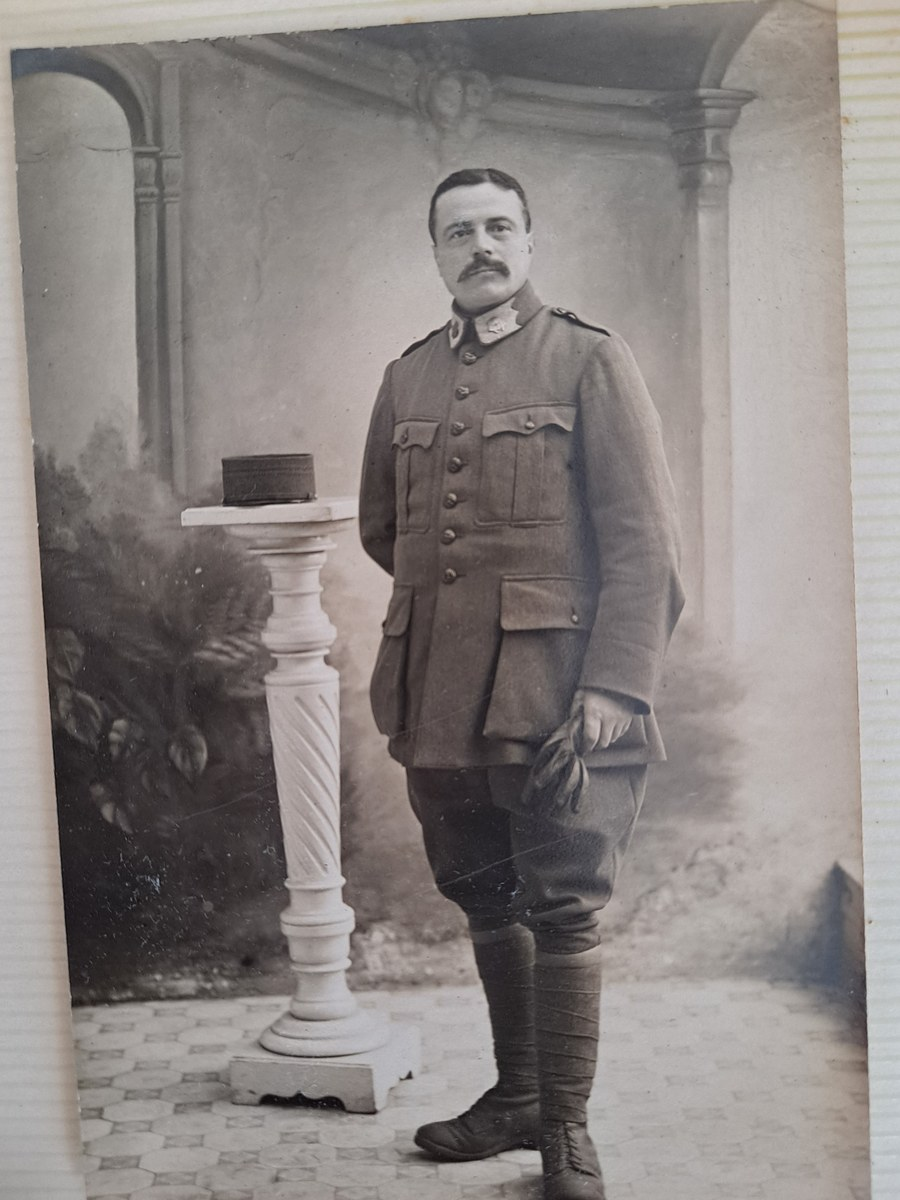
\includegraphics[width=0.94\linewidth,height=22mm,keepaspectratio]{illustrations/hippolyte_interprete_2.jpg}}
    \par\vspace{0.6mm}{\fontsize{5.8pt}{6.7pt}\selectfont Portrait en buste d'Hippolyte Combes sur le front britannique (1916--1917), portant les insignes métalliques d'interprète détaché auprès de la B.E.F.}
  \end{minipage}\hfill
  \begin{minipage}[b]{0.42\textwidth}
    \centering
    \setlength{\fboxsep}{0.7mm}\setlength{\fboxrule}{0.4pt}%
    \fcolorbox{gray!55}{white}{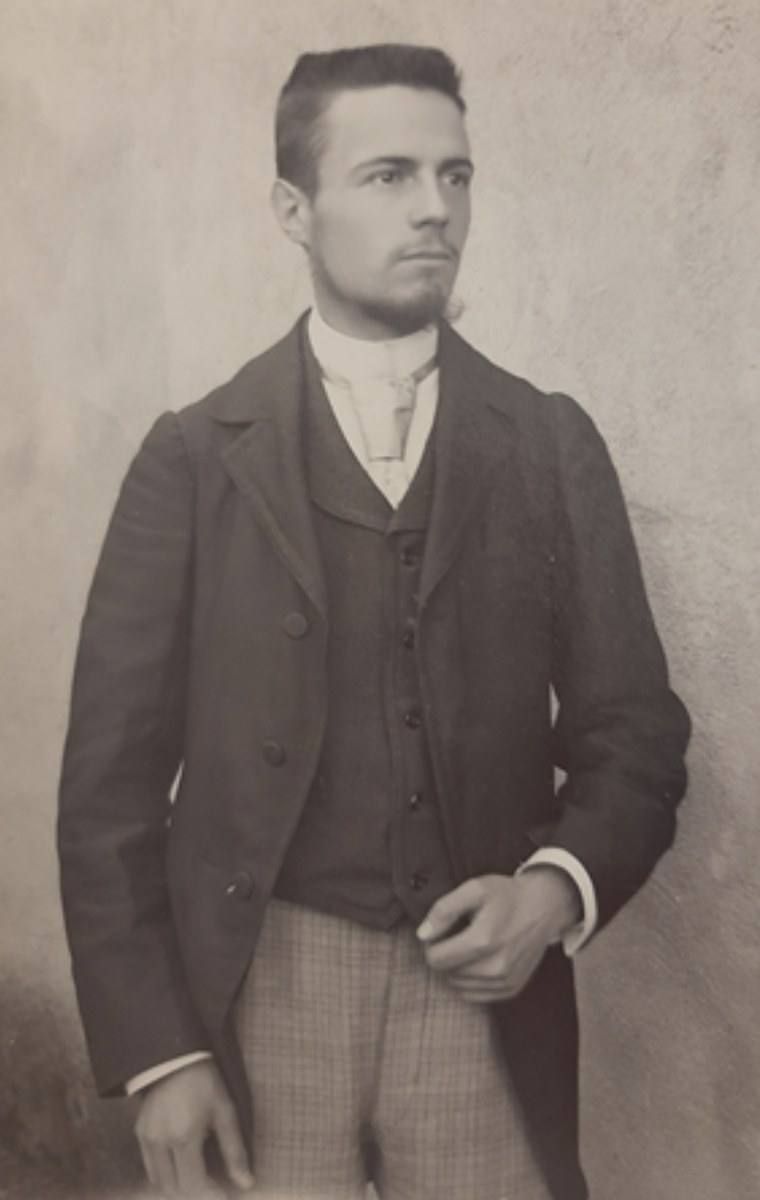
\includegraphics[width=0.94\linewidth,height=22mm,keepaspectratio]{illustrations/hippolyte_1897.jpg}}
    \par\vspace{0.6mm}{\fontsize{5.8pt}{6.7pt}\selectfont Hippolyte Combes jeune homme en 1897 (à l'âge de vingt et un ans), étudiant à Toulouse avant son séjour de quatre ans à Nottingham.}
  \end{minipage}
\end{center}
\clearpage

% =============================================================================
% VIS-A-VIS SPREAD : SCAN #019 (20251126_093618.jpg) — Vue 019
% =============================================================================
\cleardoubleevenpage
% --- En-tête du folio (Page paire / gauche : Transcription, apparat & double registre) ---
\noindent\rule{\textwidth}{0.5pt}\par\vspace{0.6mm}
\noindent\textbf{\footnotesize SCAN \#019 — VUE 019} \hfill {\scriptsize\texttt{20251126\_\allowbreak 093618.jpg}}\par\vspace{0.3mm}
\noindent{\fontsize{7.0pt}{8.2pt}\selectfont Attente vaine d'une lettre de Marguerite, « pot-au-noir » et orage sur la Lys}\par\vspace{0.25mm}
\noindent{\fontsize{7.0pt}{8.2pt}\selectfont\textit{Dimanche 13 et lundi 14 août 1916} \hfill \textit{Bac-Saint-Maur et direction d'Armentières (Nord)}}\par\vspace{0.6mm}
\noindent\rule{\textwidth}{0.35pt}\par\vspace{1.0mm}
% --- Corps de la transcription diplomatique et apparat marginal en prolongement ---
{\renewcommand{\arraystretch}{0.95}%
\noindent\hspace*{3.5mm}\begin{tabular}{@{}p{100mm}@{\hspace{3.5mm}}p{55mm}@{}}
      \leavevmode\fontsize{7.4pt}{8.6pt}\selectfont\strut 13 D – \hfill{} Aout 1916\strut & \leavevmode\fontsize{6.3pt}{7.2pt}\selectfont\raggedright\arraybackslash\color{black!88}\textbf{1} \textbf{D} \textit{dimanche}. \\
      \leavevmode\fontsize{7.4pt}{8.6pt}\selectfont\strut Soleil ardent\strut &  \\
      \leavevmode\fontsize{7.4pt}{8.6pt}\selectfont\strut Déception pénible : attendu en vain un\strut &  \\
      \leavevmode\fontsize{7.4pt}{8.6pt}\selectfont\strut mot de Margte –\strut & \leavevmode\fontsize{6.3pt}{7.2pt}\selectfont\raggedright\arraybackslash\color{black!88}\textbf{4} \textbf{Margte} \textit{Marguerite}. \\
      \leavevmode\llap{\fontsize{6.5pt}{7.5pt}\selectfont\color{darkgray}5\hspace{1.8mm}}\fontsize{7.4pt}{8.6pt}\selectfont\strut Tt le jour, pot-au-noir –\strut & \leavevmode\fontsize{6.3pt}{7.2pt}\selectfont\raggedright\arraybackslash\color{black!88}\textbf{5} \textbf{Tt} \textit{tout}. \\
      \leavevmode\fontsize{7.4pt}{8.6pt}\selectfont\strut Après-midi, venu retrouver Maurin\strut &  \\
      \leavevmode\fontsize{7.4pt}{8.6pt}\selectfont\strut et avec lui, promené campagne\strut &  \\
      \leavevmode\fontsize{7.4pt}{8.6pt}\selectfont\strut le long rivière de la Lys –\strut &  \\
      \leavevmode\fontsize{7.4pt}{8.6pt}\selectfont\strut 14 L – Ciel couvert nuages –\strut & \leavevmode\fontsize{6.3pt}{7.2pt}\selectfont\raggedright\arraybackslash\color{black!88}\textbf{9} \textbf{L} \textit{lundi}. \\
      \leavevmode\llap{\fontsize{6.5pt}{7.5pt}\selectfont\color{darkgray}10\hspace{1.8mm}}\fontsize{7.4pt}{8.6pt}\selectfont\strut Enfin, vers 1 H, pluie très forte\strut &  \\
      \leavevmode\fontsize{7.4pt}{8.6pt}\selectfont\strut rafraichi l'air — et mouille (colle\strut & \leavevmode\fontsize{6.3pt}{7.2pt}\selectfont\raggedright\arraybackslash\color{black!88}\textbf{11} \textbf{(colle} parenthèse ouverte, sans fermeture visible. \\
      \leavevmode\fontsize{7.4pt}{8.6pt}\selectfont\strut poussière routes.\strut &  \\
      \leavevmode\fontsize{7.4pt}{8.6pt}\selectfont\strut Pris plaisir à regarder averse\strut &  \\
      \leavevmode\fontsize{7.4pt}{8.6pt}\selectfont\strut zébrer air de raies obliques, à\strut &  \\
      \leavevmode\llap{\fontsize{6.5pt}{7.5pt}\selectfont\color{darkgray}15\hspace{1.8mm}}\fontsize{7.4pt}{8.6pt}\selectfont\strut écouter la pluie crépiter s/ vitre\strut & \leavevmode\fontsize{6.3pt}{7.2pt}\selectfont\raggedright\arraybackslash\color{black!88}\textbf{15} \textbf{s/} \textit{sur}. \\
      \leavevmode\fontsize{7.4pt}{8.6pt}\selectfont\strut de ma fenêtre\strut &  \\
      \leavevmode\fontsize{7.4pt}{8.6pt}\selectfont\strut Avec Lt Curtis, course à cheval\strut & \leavevmode\fontsize{6.3pt}{7.2pt}\selectfont\raggedright\arraybackslash\color{black!88}\textbf{17} \textbf{Lt} \textit{lieutenant}. \\
      \leavevmode\fontsize{7.4pt}{8.6pt}\selectfont\strut ds la direction d'Armentières —\strut & \leavevmode\fontsize{6.3pt}{7.2pt}\selectfont\raggedright\arraybackslash\color{black!88}\textbf{18} \textbf{ds} \textit{dans}. \\
      \leavevmode\fontsize{7.4pt}{8.6pt}\selectfont\strut Note de blanchissage : 50c\strut &  \\
      \leavevmode\llap{\fontsize{6.5pt}{7.5pt}\selectfont\color{darkgray}20\hspace{1.8mm}}\fontsize{7.4pt}{8.6pt}\selectfont\strut Lait : 15 c + 0.05\strut &  \\
\end{tabular}}%
\par\vspace*{\fill}
% --- Deux registres de commentaires en bas de page (sans intitulés, distingués par filets et mise en page) ---
\noindent\rule{\textwidth}{0.5pt}\par\vspace{0.8mm}
{\fontsize{6.8pt}{8.0pt}\selectfont%
\noindent\normalfont \textbf{Deux journées :} 13 D (dimanche), puis 14 L (lundi). Le trait qui suit le second en-tête sépare les journées ; le compte de blanchissage et de lait est isolé en bas par un autre filet. \textbf{l.~9--12 :} forte appartient à la pluie de la l.~10 ; la parenthèse ouverte devant colle n’a pas de fermeture visible. \textbf{l.~5 et 7--8 :} pot-au-noir est une expression figurée d’abattement ou de situation sans issue ; les ellipses promené campagne et le long rivière sont conservées sans restitutions grammaticales.\par\vspace{0.75mm}
\noindent\rule{38mm}{0.4pt}\par\vspace{0.65mm}
\noindent\hspace*{5mm}\parbox{\dimexpr\textwidth-5mm\relax}{\fontsize{6.8pt}{8.0pt}\selectfont\color{black!82}Le 14 août 1916 correspond au quarantième anniversaire de Combes selon son acte de naissance du 16 août 1876 mentionnant avant-hier. Le diariste ne signale pas l’anniversaire dans cette entrée. La sortie à cheval avec Curtis est une course, sans mission de reconnaissance explicitement donnée.}\par}
\newpage
% --- En-tête du fac-similé (Page impaire / droite : Scan original) ---
\noindent\rule{\textwidth}{0.5pt}\par\vspace{0.6mm}
\noindent\textbf{\fontsize{6.5pt}{7.6pt}\selectfont FAC-SIMILÉ EN VIS-À-VIS — VUE 019 (SCAN \#019)} \hfill {\fontsize{6.5pt}{7.6pt}\selectfont\texttt{20251126\_\allowbreak 093618.jpg}}\par\vspace{0.3mm}
\noindent{\fontsize{6.8pt}{8pt}\selectfont\textit{Livre-Journal d'Hippolyte Combes} — Dimanche 13 et lundi 14 août 1916 (Bac-Saint-Maur et direction d'Armentières (Nord))}\par\vspace{0.6mm}
\noindent\rule{\textwidth}{0.35pt}\par\vspace*{\fill}
{\centering
  \setlength{\fboxsep}{1.2mm}%
  \setlength{\fboxrule}{0.4pt}%
  \fcolorbox{gray!55}{white}{%
    \includegraphics[width=0.94\textwidth,height=0.76\textheight,keepaspectratio]{\facsimiledir/20251126_093618.jpg}%
  }\par}
\vspace*{\fill}
\noindent\rule{\textwidth}{0.35pt}\par\vspace{0.5mm}
\noindent{\fontsize{6pt}{7.1pt}\selectfont\raggedright\color{darkgray}\textbf{Source :} Archives familiales Combes — Cliché numérique \texttt{20251126\_\allowbreak 093618.jpg} (Scan \#019/186, Vue 019). Haute définition : \texttt{scans\_haute\_qualite/\allowbreak 20251126\_\allowbreak 093618.jpg} ; version allégée : \texttt{scans\_compresses/\allowbreak 20251126\_\allowbreak 093618.jpg}.\par}
\newpage

% =============================================================================
% VIS-A-VIS SPREAD : SCAN #020 (20251126_093746.jpg) — Vue 020
% =============================================================================
\cleardoubleevenpage
% --- En-tête du folio (Page paire / gauche : Transcription, apparat & double registre) ---
\noindent\rule{\textwidth}{0.5pt}\par\vspace{0.6mm}
\noindent\textbf{\footnotesize SCAN \#020 — VUE 020} \hfill {\scriptsize\texttt{20251126\_\allowbreak 093746.jpg}}\par\vspace{0.3mm}
\noindent{\fontsize{7.0pt}{8.2pt}\selectfont Journée pluvieuse du 15 août dans la mansarde et comptes de blanchissage}\par\vspace{0.25mm}
\noindent{\fontsize{7.0pt}{8.2pt}\selectfont\textit{Mardi 15 août 1916 (Assomption)} \hfill \textit{Bac-Saint-Maur / Steenwerck (Nord)}}\par\vspace{0.6mm}
\noindent\rule{\textwidth}{0.35pt}\par\vspace{1.0mm}
% --- Corps de la transcription diplomatique et apparat marginal en prolongement ---
{\renewcommand{\arraystretch}{1.02}%
\noindent\hspace*{3.5mm}\begin{tabular}{@{}p{100mm}@{\hspace{3.5mm}}p{55mm}@{}}
      \leavevmode\fontsize{7.8pt}{9.2pt}\selectfont\strut 15 Ma – Assompt. \hfill{} Aout / 16\strut & \leavevmode\fontsize{6.3pt}{7.2pt}\selectfont\raggedright\arraybackslash\color{black!88}\textbf{1} \textbf{Ma} \textit{mardi} ; \textbf{Assompt.} \textit{Assomption}. \\
      \leavevmode\fontsize{7.8pt}{9.2pt}\selectfont\strut Toute matinée et 1 peu après-midi :\strut &  \\
      \leavevmode\fontsize{7.8pt}{9.2pt}\selectfont\strut fortes ondées. Routes détrempées. Aucun\strut &  \\
      \leavevmode\fontsize{7.8pt}{9.2pt}\selectfont\strut envie aller promener. Resté partie journée\strut &  \\
      \leavevmode\llap{\fontsize{6.5pt}{7.5pt}\selectfont\color{darkgray}5\hspace{1.8mm}}\fontsize{7.8pt}{9.2pt}\selectfont\strut ds ma chambre. Large pièce : très\strut & \leavevmode\fontsize{6.3pt}{7.2pt}\selectfont\raggedright\arraybackslash\color{black!88}\textbf{5} \textbf{ds} \textit{dans}. \\
      \leavevmode\fontsize{7.8pt}{9.2pt}\selectfont\strut haute de plafond. Belle vue de la\strut &  \\
      \leavevmode\fontsize{7.8pt}{9.2pt}\selectfont\strut fenêtre, où me tiens sans cesse\strut &  \\
      \leavevmode\fontsize{7.8pt}{9.2pt}\selectfont\strut — Presque ts les matins, à l'aube,\strut & \leavevmode\fontsize{6.3pt}{7.2pt}\selectfont\raggedright\arraybackslash\color{black!88}\textbf{8} \textbf{ts} \textit{tous}. \\
      \leavevmode\fontsize{7.8pt}{9.2pt}\selectfont\strut épais brouillards\strut &  \\
      \leavevmode\llap{\fontsize{6.5pt}{7.5pt}\selectfont\color{darkgray}10\hspace{1.8mm}}\fontsize{7.8pt}{9.2pt}\selectfont\strut — Donné à ma propre, pour\strut & \leavevmode\fontsize{6.3pt}{7.2pt}\selectfont\raggedright\arraybackslash\color{black!88}\textbf{10} \textbf{propre} \textit{propriétaire}. \\
      \leavevmode\fontsize{7.8pt}{9.2pt}\selectfont\strut cooking semaine dernière et 2 l. lait : 5 f —\strut & \leavevmode\fontsize{6.3pt}{7.2pt}\selectfont\raggedright\arraybackslash\color{black!88}\textbf{11} \textbf{cooking} \textit{angl.} cuisine. \\
\end{tabular}}%
\par\vspace*{\fill}
% --- Deux registres de commentaires en bas de page (sans intitulés, distingués par filets et mise en page) ---
\noindent\rule{\textwidth}{0.5pt}\par\vspace{0.8mm}
{\fontsize{6.8pt}{8.0pt}\selectfont%
\noindent\normalfont \textbf{l.~1 :} Assompt. abrège Assomption. \textbf{l.~2--7 :} les formulations 1 peu après-midi et Aucun envie sont maintenues ; elles ne sont pas des lacunes du papier. La chambre est décrite comme haute de plafond, sans le mot mansarde. \textbf{l.~10--11 :} propre est ici la forme contractée de propriétaire ; cooking désigne la cuisine facturée avec deux litres de lait, pour 5 f au total. Ces deux lignes sont dans le corps de la page, après un tiret, sans crochet comptable.\par\vspace{0.75mm}
\noindent\rule{38mm}{0.4pt}\par\vspace{0.65mm}
\noindent\hspace*{5mm}\parbox{\dimexpr\textwidth-5mm\relax}{\fontsize{6.8pt}{8.0pt}\selectfont\color{black!82}Le 15 août est marqué Assompt. Le paiement de 5 francs réunit cooking de la semaine dernière et deux litres de lait. Il s’agit d’un règlement écrit, pas de la preuve d’un tarif hebdomadaire uniforme de pension.}\par}
\newpage
% --- En-tête du fac-similé (Page impaire / droite : Scan original) ---
\noindent\rule{\textwidth}{0.5pt}\par\vspace{0.6mm}
\noindent\textbf{\fontsize{6.5pt}{7.6pt}\selectfont FAC-SIMILÉ EN VIS-À-VIS — VUE 020 (SCAN \#020)} \hfill {\fontsize{6.5pt}{7.6pt}\selectfont\texttt{20251126\_\allowbreak 093746.jpg}}\par\vspace{0.3mm}
\noindent{\fontsize{6.8pt}{8pt}\selectfont\textit{Livre-Journal d'Hippolyte Combes} — Mardi 15 août 1916 (Assomption) (Bac-Saint-Maur / Steenwerck (Nord))}\par\vspace{0.6mm}
\noindent\rule{\textwidth}{0.35pt}\par\vspace*{\fill}
{\centering
  \setlength{\fboxsep}{1.2mm}%
  \setlength{\fboxrule}{0.4pt}%
  \fcolorbox{gray!55}{white}{%
    \includegraphics[width=0.94\textwidth,height=0.76\textheight,keepaspectratio]{\facsimiledir/20251126_093746.jpg}%
  }\par}
\vspace*{\fill}
\noindent\rule{\textwidth}{0.35pt}\par\vspace{0.5mm}
\noindent{\fontsize{6pt}{7.1pt}\selectfont\raggedright\color{darkgray}\textbf{Source :} Archives familiales Combes — Cliché numérique \texttt{20251126\_\allowbreak 093746.jpg} (Scan \#020/186, Vue 020). Haute définition : \texttt{scans\_haute\_qualite/\allowbreak 20251126\_\allowbreak 093746.jpg} ; version allégée : \texttt{scans\_compresses/\allowbreak 20251126\_\allowbreak 093746.jpg}.\par}
\newpage

% =============================================================================
% VIS-A-VIS SPREAD : SCAN #021 (20251126_093843.jpg) — Vue 021
% =============================================================================
\cleardoubleevenpage
% --- En-tête du folio (Page paire / gauche : Transcription, apparat & double registre) ---
\noindent\rule{\textwidth}{0.5pt}\par\vspace{0.6mm}
\noindent\textbf{\footnotesize SCAN \#021 — VUE 021} \hfill {\scriptsize\texttt{20251126\_\allowbreak 093843.jpg}}\par\vspace{0.3mm}
\noindent{\fontsize{7.0pt}{8.2pt}\selectfont Vendredi 18 et Samedi 19 août 1916 — Giboulées d'août, perception de la solde et chevauchée sous l'orage avec le lieutenant Curtis}\par\vspace{0.25mm}
\noindent{\fontsize{7.0pt}{8.2pt}\selectfont\textit{Vendredi 18 et samedi 19 août 1916} \hfill \textit{Steenwerck, Fleurbaix et secteur d'Armentières (Nord)}}\par\vspace{0.6mm}
\noindent\rule{\textwidth}{0.35pt}\par\vspace{1.0mm}
% --- Corps de la transcription diplomatique et apparat marginal en prolongement ---
{\renewcommand{\arraystretch}{0.95}%
\noindent\hspace*{3.5mm}\begin{tabular}{@{}p{100mm}@{\hspace{3.5mm}}p{55mm}@{}}
      \leavevmode\fontsize{7.4pt}{8.6pt}\selectfont\strut 18 Ve. \hfill{} – Aout / 16 –\strut & \leavevmode\fontsize{6.3pt}{7.2pt}\selectfont\raggedright\arraybackslash\color{black!88}\textbf{1} \textbf{Ve.} \textit{vendredi}. \\
      \leavevmode\fontsize{7.4pt}{8.6pt}\selectfont\strut Depuis 2 ou 3 jours, vraies giboulées,\strut &  \\
      \leavevmode\fontsize{7.4pt}{8.6pt}\selectfont\strut comme en mars – Averses prolongées. Puis éclaircies\strut &  \\
      \leavevmode\fontsize{7.4pt}{8.6pt}\selectfont\strut et soleil reparaît\strut &  \\
      \leavevmode\llap{\fontsize{6.5pt}{7.5pt}\selectfont\color{darkgray}5\hspace{1.8mm}}\fontsize{7.4pt}{8.6pt}\selectfont\strut Hier après-midi, au refilling point et ds 1\strut & \leavevmode\fontsize{6.3pt}{7.2pt}\selectfont\raggedright\arraybackslash\color{black!88}\textbf{5} \textbf{refilling point} \textit{angl.} point de réapprovisionnement ; \textbf{ds} \textit{dans}. \\
      \leavevmode\fontsize{7.4pt}{8.6pt}\selectfont\strut champ de trèfle, surpris par la pluie et\strut &  \\
      \leavevmode\fontsize{7.4pt}{8.6pt}\selectfont\strut mouillé j. à la peau –\strut & \leavevmode\fontsize{6.3pt}{7.2pt}\selectfont\raggedright\arraybackslash\color{black!88}\textbf{7} \textbf{j. à} \textit{jusqu’à}. \\
      \leavevmode\fontsize{7.4pt}{8.6pt}\selectfont\strut Fin journée, assez belle. Venu retrouver Maurin,\strut &  \\
      \leavevmode\fontsize{7.4pt}{8.6pt}\selectfont\strut promené ensemble et assis, pour causer\strut &  \\
      \leavevmode\llap{\fontsize{6.5pt}{7.5pt}\selectfont\color{darkgray}10\hspace{1.8mm}}\fontsize{7.4pt}{8.6pt}\selectfont\strut sur l'herbe sèche, près des lignes de ma\strut &  \\
      \leavevmode\fontsize{7.4pt}{8.6pt}\selectfont\strut Coy. \hfill{} Vers 7 H 1/2 orage\strut & \leavevmode\fontsize{6.3pt}{7.2pt}\selectfont\raggedright\arraybackslash\color{black!88}\textbf{11} \textbf{Coy.} \textit{angl.} Company, compagnie. \\
      \leavevmode\fontsize{7.4pt}{8.6pt}\selectfont\strut [ – Solde \& indemnité de fonctions : 84 fr.\strut & \leavevmode\fontsize{6.3pt}{7.2pt}\selectfont\raggedright\arraybackslash\color{black!88}\textbf{12} \textbf{[} grand crochet ouvrant à gauche du compte ; trait horizontal au-dessous. \\
      \leavevmode\fontsize{7.4pt}{8.6pt}\selectfont\strut 19 S. — Plu tte nuit —\strut & \leavevmode\fontsize{6.3pt}{7.2pt}\selectfont\raggedright\arraybackslash\color{black!88}\textbf{13} \textbf{S.} \textit{samedi} ; \textbf{tte} \textit{toute}. \\
      \leavevmode\fontsize{7.4pt}{8.6pt}\selectfont\strut Dès 8 H matin, pluie torrentielle. Routes\strut &  \\
      \leavevmode\llap{\fontsize{6.5pt}{7.5pt}\selectfont\color{darkgray}15\hspace{1.8mm}}\fontsize{7.4pt}{8.6pt}\selectfont\strut détrempées. Température rafraîchie délict.\strut & \leavevmode\fontsize{6.3pt}{7.2pt}\selectfont\raggedright\arraybackslash\color{black!88}\textbf{15} \textbf{délict.} \textit{délicieusement}. \\
      \leavevmode\fontsize{7.4pt}{8.6pt}\selectfont\strut Toute matinée et commt après-midi :\strut & \leavevmode\fontsize{6.3pt}{7.2pt}\selectfont\raggedright\arraybackslash\color{black!88}\textbf{16} \textbf{commt} \textit{commencement}. \\
      \leavevmode\fontsize{7.4pt}{8.6pt}\selectfont\strut averses très fortes — comme grêle.\strut &  \\
      \leavevmode\fontsize{7.4pt}{8.6pt}\selectfont\strut Vers 2 H 30, ce crétin de Curtis venu\strut &  \\
      \leavevmode\fontsize{7.4pt}{8.6pt}\selectfont\strut me prendre : dû l'accompagner\strut &  \\
      \leavevmode\llap{\fontsize{6.5pt}{7.5pt}\selectfont\color{darkgray}20\hspace{1.8mm}}\fontsize{7.4pt}{8.6pt}\selectfont\strut à cheval, – \& cette fois sur un bon poney.\strut &  \\
      \leavevmode\fontsize{7.4pt}{8.6pt}\selectfont\strut Longue chevauchée zone\strut &  \\
      \leavevmode\fontsize{7.4pt}{8.6pt}\selectfont\strut exposée, derrière ligne de feu\strut &  \\
\end{tabular}}%
\par\vspace*{\fill}
% --- Deux registres de commentaires en bas de page (sans intitulés, distingués par filets et mise en page) ---
\noindent\rule{\textwidth}{0.5pt}\par\vspace{0.8mm}
{\fontsize{6.8pt}{8.0pt}\selectfont%
\noindent\normalfont \textbf{l.~11--13 :} Coy. signifie Company ; lignes désigne les emplacements de la compagnie. Le compte de 84 fr. est signalé par un grand crochet ouvrant à gauche ; un trait horizontal le sépare du 19 S (samedi). Ce n’est pas une somme ajoutée en marge. \textbf{l.~15--16 :} délict. abrège délicieusement ; commt abrège commencement. \textbf{l.~18--22 :} crétin de Curtis se lit ; zone exposée, derrière ligne de feu reste une indication relative, sans localisation plus précise. Poney est un mot français, sans appel de note d’emprunt anglais.\par\vspace{0.75mm}
\noindent\rule{38mm}{0.4pt}\par\vspace{0.65mm}
\noindent\hspace*{5mm}\parbox{\dimexpr\textwidth-5mm\relax}{\fontsize{6.8pt}{8.0pt}\selectfont\color{black!82}Solde et indemnité de fonctions sont explicitement associées aux 84 francs. La chevauchée du 19 août se poursuit à la vue 022. La zone est dite exposée, derrière la ligne de feu ; sa distance aux premières tranchées n’est pas mesurée.}\par}
\newpage
% --- En-tête du fac-similé (Page impaire / droite : Scan original) ---
\noindent\rule{\textwidth}{0.5pt}\par\vspace{0.6mm}
\noindent\textbf{\fontsize{6.5pt}{7.6pt}\selectfont FAC-SIMILÉ EN VIS-À-VIS — VUE 021 (SCAN \#021)} \hfill {\fontsize{6.5pt}{7.6pt}\selectfont\texttt{20251126\_\allowbreak 093843.jpg}}\par\vspace{0.3mm}
\noindent{\fontsize{6.8pt}{8pt}\selectfont\textit{Livre-Journal d'Hippolyte Combes} — Vendredi 18 et samedi 19 août 1916 (Steenwerck, Fleurbaix et secteur d'Armentières (Nord))}\par\vspace{0.6mm}
\noindent\rule{\textwidth}{0.35pt}\par\vspace*{\fill}
{\centering
  \setlength{\fboxsep}{1.2mm}%
  \setlength{\fboxrule}{0.4pt}%
  \fcolorbox{gray!55}{white}{%
    \includegraphics[width=0.94\textwidth,height=0.76\textheight,keepaspectratio]{\facsimiledir/20251126_093843.jpg}%
  }\par}
\vspace*{\fill}
\noindent\rule{\textwidth}{0.35pt}\par\vspace{0.5mm}
\noindent{\fontsize{6pt}{7.1pt}\selectfont\raggedright\color{darkgray}\textbf{Source :} Archives familiales Combes — Cliché numérique \texttt{20251126\_\allowbreak 093843.jpg} (Scan \#021/186, Vue 021). Haute définition : \texttt{scans\_haute\_qualite/\allowbreak 20251126\_\allowbreak 093843.jpg} ; version allégée : \texttt{scans\_compresses/\allowbreak 20251126\_\allowbreak 093843.jpg}.\par}
\newpage

% =============================================================================
% VIS-A-VIS SPREAD : SCAN #022 (20251126_093857.jpg) — Vue 022
% =============================================================================
\cleardoubleevenpage
% --- En-tête du folio (Page paire / gauche : Transcription, apparat & double registre) ---
\noindent\rule{\textwidth}{0.5pt}\par\vspace{0.6mm}
\noindent\textbf{\footnotesize SCAN \#022 — VUE 022} \hfill {\scriptsize\texttt{20251126\_\allowbreak 093857.jpg}}\par\vspace{0.3mm}
\noindent{\fontsize{7.0pt}{8.2pt}\selectfont Traversée de Fleurbaix et d'Armentières dévastées par les obus}\par\vspace{0.25mm}
\noindent{\fontsize{7.0pt}{8.2pt}\selectfont\textit{Samedi 19 août 1916 (suite)} \hfill \textit{Erquinghem-Lys, Fleurbaix et Armentières (Pas-de-Calais / Nord)}}\par\vspace{0.6mm}
\noindent\rule{\textwidth}{0.35pt}\par\vspace{1.0mm}
% --- Corps de la transcription diplomatique et apparat marginal en prolongement ---
{\renewcommand{\arraystretch}{0.89}%
\noindent\hspace*{3.5mm}\begin{tabular}{@{}p{100mm}@{\hspace{3.5mm}}p{55mm}@{}}
      \leavevmode\fontsize{7.0pt}{8.1pt}\selectfont\strut et galop à travers champs \hfill{} 19 Sam –\strut & \leavevmode\fontsize{6.3pt}{7.2pt}\selectfont\raggedright\arraybackslash\color{black!88}\textbf{1} \textbf{Sam} \textit{samedi}. \\
      \leavevmode\fontsize{7.0pt}{8.1pt}\selectfont\strut et arrivé j. à la blanchisserie Barbry\strut & \leavevmode\fontsize{6.3pt}{7.2pt}\selectfont\raggedright\arraybackslash\color{black!88}\textbf{2} \textbf{j. à} \textit{jusqu’à}. \\
      \leavevmode\fontsize{7.0pt}{8.1pt}\selectfont\strut Puis dirigé sur Fleurbaix. Au centre du\strut &  \\
      \leavevmode\fontsize{7.0pt}{8.1pt}\selectfont\strut village (tourné à dr.) et remonté lentement rue\strut & \leavevmode\fontsize{6.3pt}{7.2pt}\selectfont\raggedright\arraybackslash\color{black!88}\textbf{4} \textbf{dr.} \textit{droite}. \\
      \leavevmode\llap{\fontsize{6.5pt}{7.5pt}\selectfont\color{darkgray}5\hspace{1.8mm}}\fontsize{7.0pt}{8.1pt}\selectfont\strut dont presque ttes les maisons ont reçu des\strut & \leavevmode\fontsize{6.3pt}{7.2pt}\selectfont\raggedright\arraybackslash\color{black!88}\textbf{5} \textbf{ttes} \textit{toutes}. \\
      \leavevmode\fontsize{7.0pt}{8.1pt}\selectfont\strut obus. –\strut &  \\
      \leavevmode\fontsize{7.0pt}{8.1pt}\selectfont\strut Continué ensuite sur Armentières\strut &  \\
      \leavevmode\fontsize{7.0pt}{8.1pt}\selectfont\strut Arrivé par gare (l. est complt déserte)\strut & \leavevmode\fontsize{6.3pt}{7.2pt}\selectfont\raggedright\arraybackslash\color{black!88}\textbf{8} \textbf{l.} \textit{laquelle} ; \textbf{complt} \textit{complètement}. \\
      \leavevmode\fontsize{7.0pt}{8.1pt}\selectfont\strut Parcouru principaux quartiers.\strut &  \\
      \leavevmode\llap{\fontsize{6.5pt}{7.5pt}\selectfont\color{darkgray}10\hspace{1.8mm}}\fontsize{7.0pt}{8.1pt}\selectfont\strut Ville importante, riche — très b. maisons\strut & \leavevmode\fontsize{6.3pt}{7.2pt}\selectfont\raggedright\arraybackslash\color{black!88}\textbf{10} \textbf{b.} \textit{belles}. \\
      \leavevmode\fontsize{7.0pt}{8.1pt}\selectfont\strut Effets des bombardements : grands\strut &  \\
      \leavevmode\fontsize{7.0pt}{8.1pt}\selectfont\strut dommages. Vu, çà \& là, de toits\strut &  \\
      \leavevmode\fontsize{7.0pt}{8.1pt}\selectfont\strut crevés, de façades trouées, cloisons\strut &  \\
      \leavevmode\fontsize{7.0pt}{8.1pt}\selectfont\strut d'appartement mises à nu –\strut &  \\
      \leavevmode\llap{\fontsize{6.5pt}{7.5pt}\selectfont\color{darkgray}15\hspace{1.8mm}}\fontsize{7.0pt}{8.1pt}\selectfont\strut Église à briques rouges, sur 1 place\strut &  \\
      \leavevmode\fontsize{7.0pt}{8.1pt}\selectfont\strut très atteinte. Clocher découronné\strut &  \\
      \leavevmode\fontsize{7.0pt}{8.1pt}\selectfont\strut Toiture abattue\strut &  \\
      \leavevmode\fontsize{7.0pt}{8.1pt}\selectfont\strut La + des immeubles inoccupés,\strut & \leavevmode\fontsize{6.3pt}{7.2pt}\selectfont\raggedright\arraybackslash\color{black!88}\textbf{18} \textbf{La +} la plupart, selon la syntaxe. \\
      \leavevmode\fontsize{7.0pt}{8.1pt}\selectfont\strut abandonnés par leurs habitants.\strut &  \\
      \leavevmode\llap{\fontsize{6.5pt}{7.5pt}\selectfont\color{darkgray}20\hspace{1.8mm}}\fontsize{7.0pt}{8.1pt}\selectfont\strut Écossais\strut & \leavevmode\fontsize{6.3pt}{7.2pt}\selectfont\raggedright\arraybackslash\color{black!88}\textbf{20} \textbf{Écossais} ajout au-dessus de Rentrés ; rattachement incertain. \\
      \leavevmode\fontsize{7.0pt}{8.1pt}\selectfont\strut Rentrés par Gde route – Arrêté à\strut & \leavevmode\fontsize{6.3pt}{7.2pt}\selectfont\raggedright\arraybackslash\color{black!88}\textbf{21} \textbf{Gde} \textit{grande}. \\
      \leavevmode\fontsize{7.0pt}{8.1pt}\selectfont\strut Erquinghem et thé avec 1 off des Sussex\strut & \leavevmode\fontsize{6.3pt}{7.2pt}\selectfont\raggedright\arraybackslash\color{black!88}\textbf{22} \textbf{off} \textit{officier}. \\
      \leavevmode\fontsize{7.0pt}{8.1pt}\selectfont\strut Fin journée ensoleillée et\strut &  \\
      \leavevmode\fontsize{7.0pt}{8.1pt}\selectfont\strut très belle.\strut &  \\
\end{tabular}}%
\par\vspace*{\fill}
% --- Deux registres de commentaires en bas de page (sans intitulés, distingués par filets et mise en page) ---
\noindent\rule{\textwidth}{0.5pt}\par\vspace{0.8mm}
{\fontsize{6.8pt}{8.0pt}\selectfont%
\noindent\normalfont \textbf{Continuation du 19 août :} l’en-tête 19 Sam est placé à droite de la première ligne, qui poursuit la chevauchée de la vue précédente. \textbf{l.~8 et 18 :} l. renvoie à la gare (laquelle) ; La + se comprend la plupart, sans développer ces formes dans la transcription. \textbf{l.~20 :} Écossais est un ajout d’encre plus faible au-dessus de Rentrés ; son rattachement syntaxique reste incertain. \textbf{l.~11--17 :} le constat des destructions est conservé, avec ses ellipses, sans reconstruire une phrase plus régulière.\par\vspace{0.75mm}
\noindent\rule{38mm}{0.4pt}\par\vspace{0.65mm}
\noindent\hspace*{5mm}\parbox{\dimexpr\textwidth-5mm\relax}{\fontsize{6.8pt}{8.0pt}\selectfont\color{black!82}Fleurbaix, Armentières et Erquinghem sont des étapes nommées. L’église endommagée n’est pas nommée ; Saint-Vaast et Notre-Dame ne peuvent devenir des identifications acquises sur cette seule description. Sussex désigne ici l’appartenance rapportée de l’officier rencontré, sans numéro de bataillon.}\par}
\newpage
% --- En-tête du fac-similé (Page impaire / droite : Scan original) ---
\noindent\rule{\textwidth}{0.5pt}\par\vspace{0.6mm}
\noindent\textbf{\fontsize{6.5pt}{7.6pt}\selectfont FAC-SIMILÉ EN VIS-À-VIS — VUE 022 (SCAN \#022)} \hfill {\fontsize{6.5pt}{7.6pt}\selectfont\texttt{20251126\_\allowbreak 093857.jpg}}\par\vspace{0.3mm}
\noindent{\fontsize{6.8pt}{8pt}\selectfont\textit{Livre-Journal d'Hippolyte Combes} — Samedi 19 août 1916 (suite) (Erquinghem-Lys, Fleurbaix et Armentières (Pas-de-Calais / Nord))}\par\vspace{0.6mm}
\noindent\rule{\textwidth}{0.35pt}\par\vspace*{\fill}
{\centering
  \setlength{\fboxsep}{1.2mm}%
  \setlength{\fboxrule}{0.4pt}%
  \fcolorbox{gray!55}{white}{%
    \includegraphics[width=0.94\textwidth,height=0.76\textheight,keepaspectratio]{\facsimiledir/20251126_093857.jpg}%
  }\par}
\vspace*{\fill}
\noindent\rule{\textwidth}{0.35pt}\par\vspace{0.5mm}
\noindent{\fontsize{6pt}{7.1pt}\selectfont\raggedright\color{darkgray}\textbf{Source :} Archives familiales Combes — Cliché numérique \texttt{20251126\_\allowbreak 093857.jpg} (Scan \#022/186, Vue 022). Haute définition : \texttt{scans\_haute\_qualite/\allowbreak 20251126\_\allowbreak 093857.jpg} ; version allégée : \texttt{scans\_compresses/\allowbreak 20251126\_\allowbreak 093857.jpg}.\par}
\newpage

% =============================================================================
% VIS-A-VIS SPREAD : SCAN #023 (20251126_093922.jpg) — Vue 023
% =============================================================================
\cleardoubleevenpage
% --- En-tête du folio (Page paire / gauche : Transcription, apparat & double registre) ---
\noindent\rule{\textwidth}{0.5pt}\par\vspace{0.6mm}
\noindent\textbf{\footnotesize SCAN \#023 — VUE 023} \hfill {\scriptsize\texttt{20251126\_\allowbreak 093922.jpg}}\par\vspace{0.3mm}
\noindent{\fontsize{7.0pt}{8.2pt}\selectfont Café chez M. Barbry avec les adjudants Lupin et Schumacher et préparatifs de départ}\par\vspace{0.25mm}
\noindent{\fontsize{7.0pt}{8.2pt}\selectfont\textit{Dimanche 20 et lundi 21 août 1916} \hfill \textit{Erquinghem-Lys et Steenwerck (Nord)}}\par\vspace{0.6mm}
\noindent\rule{\textwidth}{0.35pt}\par\vspace{1.0mm}
% --- Corps de la transcription diplomatique et apparat marginal en prolongement ---
{\renewcommand{\arraystretch}{0.89}%
\noindent\hspace*{3.5mm}\begin{tabular}{@{}p{100mm}@{\hspace{3.5mm}}p{55mm}@{}}
      \leavevmode\fontsize{7.0pt}{8.1pt}\selectfont\strut 20 D – \hfill{} Aout 1916\strut & \leavevmode\fontsize{6.3pt}{7.2pt}\selectfont\raggedright\arraybackslash\color{black!88}\textbf{1} \textbf{D} \textit{dimanche}. \\
      \leavevmode\fontsize{7.0pt}{8.1pt}\selectfont\strut Tour à tour averses \& sunshine\strut & \leavevmode\fontsize{6.3pt}{7.2pt}\selectfont\raggedright\arraybackslash\color{black!88}\textbf{2} \textbf{sunshine} \textit{angl.} soleil, éclaircies de soleil. \\
      \leavevmode\fontsize{7.0pt}{8.1pt}\selectfont\strut Partie de l'après-midi : assez beau –\strut &  \\
      \leavevmode\fontsize{7.0pt}{8.1pt}\selectfont\strut Avec cet idiot de Ctis, to the fields for\strut & \leavevmode\fontsize{6.3pt}{7.2pt}\selectfont\raggedright\arraybackslash\color{black!88}\textbf{4} \textbf{Ctis} \textit{Curtis} ; \textbf{to the fields for} \textit{angl.} avec green forage à la ligne suivante : aux champs chercher du fourrage vert. \\
      \leavevmode\llap{\fontsize{6.5pt}{7.5pt}\selectfont\color{darkgray}5\hspace{1.8mm}}\fontsize{7.0pt}{8.1pt}\selectfont\strut green forage, puis, café et rhum chez\strut & \leavevmode\fontsize{6.3pt}{7.2pt}\selectfont\raggedright\arraybackslash\color{black!88}\textbf{5} \textbf{green forage} \textit{angl.} fourrage vert. \\
      \leavevmode\fontsize{7.0pt}{8.1pt}\selectfont\strut le propre, M. Barbry — y $[\![$[illis.]$]\!]$ amené\strut & \leavevmode\fontsize{6.3pt}{7.2pt}\selectfont\raggedright\arraybackslash\color{black!88}\textbf{6} \textbf{propre} \textit{propriétaire} ; \textbf{$[\![$[illis.]$]\!]$} suppression dont le texte reste non déchiffré. \\
      \leavevmode\fontsize{7.0pt}{8.1pt}\selectfont\strut adjudants Lupin \& Schumacher\strut &  \\
      \leavevmode\fontsize{7.0pt}{8.1pt}\selectfont\strut Bien reposé chambre fin journée\strut &  \\
      \leavevmode\fontsize{7.0pt}{8.1pt}\selectfont\strut Moral devenu excellent. Réagi contre\strut &  \\
      \leavevmode\llap{\fontsize{6.5pt}{7.5pt}\selectfont\color{darkgray}10\hspace{1.8mm}}\fontsize{7.0pt}{8.1pt}\selectfont\strut dépression des jours précédents. Me $[\![$[illis.]$]\!]$\strut & \leavevmode\fontsize{6.3pt}{7.2pt}\selectfont\raggedright\arraybackslash\color{black!88}\textbf{10} \textbf{$[\![$[illis.]$]\!]$} suppression dont le texte reste non déchiffré. \\
      \leavevmode\fontsize{7.0pt}{8.1pt}\selectfont\strut prépare déjà départ semaine prochaine\strut &  \\
      \leavevmode\fontsize{7.0pt}{8.1pt}\selectfont\strut de ma fenêtre : haute \& large, découvre\strut &  \\
      \leavevmode\fontsize{7.0pt}{8.1pt}\selectfont\strut gd horizon : prairies, champs, boqueteaux\strut & \leavevmode\fontsize{6.3pt}{7.2pt}\selectfont\raggedright\arraybackslash\color{black!88}\textbf{13} \textbf{gd} \textit{grand}. \\
      \leavevmode\fontsize{7.0pt}{8.1pt}\selectfont\strut Paysage d’ 1 banalité \& platitude extrême\strut &  \\
      \leavevmode\llap{\fontsize{6.5pt}{7.5pt}\selectfont\color{darkgray}15\hspace{1.8mm}}\fontsize{7.0pt}{8.1pt}\selectfont\strut 21 L. Journée very belle. Soleil, brillé\strut & \leavevmode\fontsize{6.3pt}{7.2pt}\selectfont\raggedright\arraybackslash\color{black!88}\textbf{15} \textbf{L.} \textit{lundi} ; \textbf{very belle} \textit{hybr.} très belle ; very est anglais, belle français. \\
      \leavevmode\fontsize{7.0pt}{8.1pt}\selectfont\strut matin \& soir. Ciel couvert pendant 1 c. temps\strut & \leavevmode\fontsize{6.3pt}{7.2pt}\selectfont\raggedright\arraybackslash\color{black!88}\textbf{16} \textbf{c.} \textit{certain}. \\
      \leavevmode\fontsize{7.0pt}{8.1pt}\selectfont\strut Fin jour très belle mervx sunset, que\strut & \leavevmode\fontsize{6.3pt}{7.2pt}\selectfont\raggedright\arraybackslash\color{black!88}\textbf{17} \textbf{mervx} \textit{merveilleux} ; \textbf{sunset} \textit{angl.} coucher du soleil. \\
      \leavevmode\fontsize{7.0pt}{8.1pt}\selectfont\strut j'ai admiré de ma fenêtre. Lignes de\strut &  \\
      \leavevmode\fontsize{7.0pt}{8.1pt}\selectfont\strut nuages frangés d'or étincelant\strut &  \\
      \leavevmode\llap{\fontsize{6.5pt}{7.5pt}\selectfont\color{darkgray}20\hspace{1.8mm}}\fontsize{7.0pt}{8.1pt}\selectfont\strut Allégé mes bagages en\strut &  \\
      \leavevmode\fontsize{7.0pt}{8.1pt}\selectfont\strut expédiant 1 sac à Nogent.\strut &  \\
      \leavevmode\fontsize{7.0pt}{8.1pt}\selectfont\strut Matin, venu à cheval à Steenwerk\strut &  \\
      \leavevmode\fontsize{7.0pt}{8.1pt}\selectfont\strut [ — A Proprie : 5 f (cooking, washing, \& eggs)\strut & \leavevmode\fontsize{6.3pt}{7.2pt}\selectfont\raggedright\arraybackslash\color{black!88}\textbf{23} \textbf{[} crochet ouvrant à gauche des dépenses des deux dernières lignes ; \textbf{Proprie} \textit{propriétaire} ; \textbf{cooking} \textit{angl.} cuisine ; \textbf{washing} \textit{angl.} lavage du linge ; \textbf{eggs} \textit{angl.} œufs. \\
      \leavevmode\fontsize{7.0pt}{8.1pt}\selectfont\strut A mon groom : 2 f – Varia : 10 c –\strut & \leavevmode\fontsize{6.3pt}{7.2pt}\selectfont\raggedright\arraybackslash\color{black!88}\textbf{24} \textbf{groom} \textit{angl.} palefrenier ; \textbf{Varia} \textit{lat.} dépenses diverses. \\
\end{tabular}}%
\par\vspace*{\fill}
% --- Deux registres de commentaires en bas de page (sans intitulés, distingués par filets et mise en page) ---
\noindent\rule{\textwidth}{0.5pt}\par\vspace{0.8mm}
{\fontsize{6.8pt}{8.0pt}\selectfont%
\noindent\normalfont \textbf{l.~6 et 10 :} deux séquences biffées précèdent amené et prépare. La seconde peut évoquer fais à, mais son contenu n’est pas établi ; les doubles crochets encadrent les suppressions, non des lacunes matérielles. \textbf{l.~4--5 et 15 :} to the fields for green forage forme une locution continue sur deux lignes ; very belle mêle anglais et français. \textbf{l.~23--24 :} un crochet ouvrant à gauche regroupe les dépenses, dans le bas de la page ; les gloses de propriétaire, des termes anglais et de Varia manquaient ou étaient partielles.\par\vspace{0.75mm}
\noindent\rule{38mm}{0.4pt}\par\vspace{0.65mm}
\noindent\hspace*{5mm}\parbox{\dimexpr\textwidth-5mm\relax}{\fontsize{6.8pt}{8.0pt}\selectfont\color{black!82}Le propriétaire Barbry et les adjudants Lupin/Schumacher sont nommés. Une identité avec les personnes d’autres occurrences reste à confronter à leurs graphies et aux pièces de correspondance. Le sac envoyé à Nogent est écrit ; une adresse précise n’apparaît pas ici.}\par}
\newpage
% --- En-tête du fac-similé (Page impaire / droite : Scan original) ---
\noindent\rule{\textwidth}{0.5pt}\par\vspace{0.6mm}
\noindent\textbf{\fontsize{6.5pt}{7.6pt}\selectfont FAC-SIMILÉ EN VIS-À-VIS — VUE 023 (SCAN \#023)} \hfill {\fontsize{6.5pt}{7.6pt}\selectfont\texttt{20251126\_\allowbreak 093922.jpg}}\par\vspace{0.3mm}
\noindent{\fontsize{6.8pt}{8pt}\selectfont\textit{Livre-Journal d'Hippolyte Combes} — Dimanche 20 et lundi 21 août 1916 (Erquinghem-Lys et Steenwerck (Nord))}\par\vspace{0.6mm}
\noindent\rule{\textwidth}{0.35pt}\par\vspace*{\fill}
{\centering
  \setlength{\fboxsep}{1.2mm}%
  \setlength{\fboxrule}{0.4pt}%
  \fcolorbox{gray!55}{white}{%
    \includegraphics[width=0.94\textwidth,height=0.76\textheight,keepaspectratio]{\facsimiledir/20251126_093922.jpg}%
  }\par}
\vspace*{\fill}
\noindent\rule{\textwidth}{0.35pt}\par\vspace{0.5mm}
\noindent{\fontsize{6pt}{7.1pt}\selectfont\raggedright\color{darkgray}\textbf{Source :} Archives familiales Combes — Cliché numérique \texttt{20251126\_\allowbreak 093922.jpg} (Scan \#023/186, Vue 023). Haute définition : \texttt{scans\_haute\_qualite/\allowbreak 20251126\_\allowbreak 093922.jpg} ; version allégée : \texttt{scans\_compresses/\allowbreak 20251126\_\allowbreak 093922.jpg}.\par}
\newpage

% =============================================================================
% VIS-A-VIS SPREAD : SCAN #024 (20251126_093941.jpg) — Vue 024
% =============================================================================
\cleardoubleevenpage
% --- En-tête du folio (Page paire / gauche : Transcription, apparat & double registre) ---
\noindent\rule{\textwidth}{0.5pt}\par\vspace{0.6mm}
\noindent\textbf{\footnotesize SCAN \#024 — VUE 024} \hfill {\scriptsize\texttt{20251126\_\allowbreak 093941.jpg}}\par\vspace{0.3mm}
\noindent{\fontsize{7.0pt}{8.2pt}\selectfont Mardi 22 août 1916 — Bière chez un charcutier avec Maurin évoquant les beautés d'Antibes et envoi d’un sac de linge à Nogent}\par\vspace{0.25mm}
\noindent{\fontsize{7.0pt}{8.2pt}\selectfont\textit{Mardi 22 août 1916} \hfill \textit{Steenwerck, Bac-Saint-Maur et Erquinghem-Lys (Nord)}}\par\vspace{0.6mm}
\noindent\rule{\textwidth}{0.35pt}\par\vspace{1.0mm}
% --- Corps de la transcription diplomatique et apparat marginal en prolongement ---
{\renewcommand{\arraystretch}{1.02}%
\noindent\hspace*{3.5mm}\begin{tabular}{@{}p{100mm}@{\hspace{3.5mm}}p{55mm}@{}}
      \leavevmode\fontsize{7.8pt}{9.2pt}\selectfont\strut 22 Ma \hfill{} Aout / 16\strut & \leavevmode\fontsize{6.3pt}{7.2pt}\selectfont\raggedright\arraybackslash\color{black!88}\textbf{1} \textbf{Ma} \textit{mardi}. \\
      \leavevmode\fontsize{7.8pt}{9.2pt}\selectfont\strut Ciel nuageux – s'est tt à fait éclairci\strut & \leavevmode\fontsize{6.3pt}{7.2pt}\selectfont\raggedright\arraybackslash\color{black!88}\textbf{2} \textbf{tt} \textit{tout}. \\
      \leavevmode\fontsize{7.8pt}{9.2pt}\selectfont\strut après-midi et très beau soleil\strut &  \\
      \leavevmode\fontsize{7.8pt}{9.2pt}\selectfont\strut Venu à pied à Steenwerck : 55 m.\strut &  \\
      \leavevmode\llap{\fontsize{6.5pt}{7.5pt}\selectfont\color{darkgray}5\hspace{1.8mm}}\fontsize{7.8pt}{9.2pt}\selectfont\strut Promenade lente, très agréable\strut &  \\
      \leavevmode\fontsize{7.8pt}{9.2pt}\selectfont\strut Vers 5H 1/2, retrouvé Maurin, et allés\strut &  \\
      \leavevmode\fontsize{7.8pt}{9.2pt}\selectfont\strut ensemble à Bac St-Maur. En savourant\strut & \leavevmode\fontsize{6.3pt}{7.2pt}\selectfont\raggedright\arraybackslash\color{black!88}\textbf{7} \textbf{St} \textit{Saint}. \\
      \leavevmode\fontsize{7.8pt}{9.2pt}\selectfont\strut bonne bière ds coquette salle à manger\strut & \leavevmode\fontsize{6.3pt}{7.2pt}\selectfont\raggedright\arraybackslash\color{black!88}\textbf{8} \textbf{ds} \textit{dans}. \\
      \leavevmode\fontsize{7.8pt}{9.2pt}\selectfont\strut chz 1 charcutier, causé Provence. Maurin\strut & \leavevmode\fontsize{6.3pt}{7.2pt}\selectfont\raggedright\arraybackslash\color{black!88}\textbf{9} \textbf{chz} \textit{chez}. \\
      \leavevmode\llap{\fontsize{6.5pt}{7.5pt}\selectfont\color{darkgray}10\hspace{1.8mm}}\fontsize{7.8pt}{9.2pt}\selectfont\strut m'a décrit av. lyrisme beautés d'Antibes.\strut & \leavevmode\fontsize{6.3pt}{7.2pt}\selectfont\raggedright\arraybackslash\color{black!88}\textbf{10} \textbf{av.} \textit{avec}. \\
      \leavevmode\fontsize{7.8pt}{9.2pt}\selectfont\strut Magnifique sunset\strut & \leavevmode\fontsize{6.3pt}{7.2pt}\selectfont\raggedright\arraybackslash\color{black!88}\textbf{11} \textbf{sunset} \textit{angl.} coucher du soleil. \\
      \leavevmode\fontsize{7.8pt}{9.2pt}\selectfont\strut — Fait expédier par 1 commre d'Erquinghem\strut & \leavevmode\fontsize{6.3pt}{7.2pt}\selectfont\raggedright\arraybackslash\color{black!88}\textbf{12} \textbf{commre} \textit{commissionnaire}. \\
      \leavevmode\fontsize{7.8pt}{9.2pt}\selectfont\strut 1 sac linge à Nogent, par gare de\strut & \leavevmode\fontsize{6.3pt}{7.2pt}\selectfont\raggedright\arraybackslash\color{black!88}\textbf{13} \textbf{1 sac linge} début du groupe de dépenses signalé par un crochet ouvrant à gauche. \\
      \leavevmode\fontsize{7.8pt}{9.2pt}\selectfont\strut Steenwerck : 13 kgs; 3f 80; factage à l'arrivée\strut &  \\
      \leavevmode\llap{\fontsize{6.5pt}{7.5pt}\selectfont\color{darkgray}15\hspace{1.8mm}}\fontsize{7.8pt}{9.2pt}\selectfont\strut compris (40c). – Emballage au départ : 50c\strut &  \\
      \leavevmode\fontsize{7.8pt}{9.2pt}\selectfont\strut Cartes ples à Steenwerck : 30 c\strut & \leavevmode\fontsize{6.3pt}{7.2pt}\selectfont\raggedright\arraybackslash\color{black!88}\textbf{16} \textbf{Cartes ples} \textit{cartes postales}. \\
      \leavevmode\fontsize{7.8pt}{9.2pt}\selectfont\strut Varia : 10 c\strut & \leavevmode\fontsize{6.3pt}{7.2pt}\selectfont\raggedright\arraybackslash\color{black!88}\textbf{17} \textbf{Varia} \textit{lat.} dépenses diverses. \\
      \leavevmode\fontsize{7.8pt}{9.2pt}\selectfont\strut Bain : 1 f 25\strut &  \\
\end{tabular}}%
\par\vspace*{\fill}
% --- Deux registres de commentaires en bas de page (sans intitulés, distingués par filets et mise en page) ---
\noindent\rule{\textwidth}{0.5pt}\par\vspace{0.8mm}
{\fontsize{6.8pt}{8.0pt}\selectfont%
\noindent\normalfont \textbf{l.~12--18 :} commre abrège commissionnaire. Le récit de l’expédition se prolonge dans les comptes, signalés à gauche par un grand crochet ouvrant. Le transport porte sur un sac de linge (13 kgs), pour 3 f 80, factage à l’arrivée compris (40 c) ; l’emballage au départ est un poste distinct de 50 c. Emballage est préférable à Timbrage : attaque E, jambages m, b haut et finale allage. Les autres dépenses sont les cartes postales, Varia et le bain ; elles ne sont pas les frais d’un voyage du diariste.\par\vspace{0.75mm}
\noindent\rule{38mm}{0.4pt}\par\vspace{0.65mm}
\noindent\hspace*{5mm}\parbox{\dimexpr\textwidth-5mm\relax}{\fontsize{6.8pt}{8.0pt}\selectfont\color{black!82}Entretien avec Maurin au sujet de la Provence et d’Antibes ; envoi du sac de 13 kgs par Steenwerck. Le compte distingue 3 f 80, le factage 40 c compris et l’emballage 50 c au départ. L’ancienne explication par un timbre de récépissé ne correspond plus à la lecture Emballage.}\par}
\newpage
% --- En-tête du fac-similé (Page impaire / droite : Scan original) ---
\noindent\rule{\textwidth}{0.5pt}\par\vspace{0.6mm}
\noindent\textbf{\fontsize{6.5pt}{7.6pt}\selectfont FAC-SIMILÉ EN VIS-À-VIS — VUE 024 (SCAN \#024)} \hfill {\fontsize{6.5pt}{7.6pt}\selectfont\texttt{20251126\_\allowbreak 093941.jpg}}\par\vspace{0.3mm}
\noindent{\fontsize{6.8pt}{8pt}\selectfont\textit{Livre-Journal d'Hippolyte Combes} — Mardi 22 août 1916 (Steenwerck, Bac-Saint-Maur et Erquinghem-Lys (Nord))}\par\vspace{0.6mm}
\noindent\rule{\textwidth}{0.35pt}\par\vspace*{\fill}
{\centering
  \setlength{\fboxsep}{1.2mm}%
  \setlength{\fboxrule}{0.4pt}%
  \fcolorbox{gray!55}{white}{%
    \includegraphics[width=0.94\textwidth,height=0.76\textheight,keepaspectratio]{\facsimiledir/20251126_093941.jpg}%
  }\par}
\vspace*{\fill}
\noindent\rule{\textwidth}{0.35pt}\par\vspace{0.5mm}
\noindent{\fontsize{6pt}{7.1pt}\selectfont\raggedright\color{darkgray}\textbf{Source :} Archives familiales Combes — Cliché numérique \texttt{20251126\_\allowbreak 093941.jpg} (Scan \#024/186, Vue 024). Haute définition : \texttt{scans\_haute\_qualite/\allowbreak 20251126\_\allowbreak 093941.jpg} ; version allégée : \texttt{scans\_compresses/\allowbreak 20251126\_\allowbreak 093941.jpg}.\par}
\newpage

% =============================================================================
% VIS-A-VIS SPREAD : SCAN #025 (20251126_093955.jpg) — Vue 025
% =============================================================================
\cleardoubleevenpage
% --- En-tête du folio (Page paire / gauche : Transcription, apparat & double registre) ---
\noindent\rule{\textwidth}{0.5pt}\par\vspace{0.6mm}
\noindent\textbf{\footnotesize SCAN \#025 — VUE 025} \hfill {\scriptsize\texttt{20251126\_\allowbreak 093955.jpg}}\par\vspace{0.3mm}
\noindent{\fontsize{7.0pt}{8.2pt}\selectfont Chevauchée jusqu'à Estaires : l'église Saint-Vaast, l'Hôtel de Ville et l'hygiène par l'exercice}\par\vspace{0.25mm}
\noindent{\fontsize{7.0pt}{8.2pt}\selectfont\textit{Mercredi 23 août 1916} \hfill \textit{Estaires (Nord)}}\par\vspace{0.6mm}
\noindent\rule{\textwidth}{0.35pt}\par\vspace{1.0mm}
% --- Corps de la transcription diplomatique et apparat marginal en prolongement ---
{\renewcommand{\arraystretch}{0.95}%
\noindent\hspace*{3.5mm}\begin{tabular}{@{}p{100mm}@{\hspace{3.5mm}}p{55mm}@{}}
      \leavevmode\fontsize{7.4pt}{8.6pt}\selectfont\strut 23 Merc \hfill{} Aout / 16\strut & \leavevmode\fontsize{6.3pt}{7.2pt}\selectfont\raggedright\arraybackslash\color{black!88}\textbf{1} \textbf{Merc} \textit{mercredi}. \\
      \leavevmode\fontsize{7.4pt}{8.6pt}\selectfont\strut Temps couvert, matinée et surtout\strut &  \\
      \leavevmode\fontsize{7.4pt}{8.6pt}\selectfont\strut fin journée – Dès 6H 1/2, cme 1 légère\strut & \leavevmode\fontsize{6.3pt}{7.2pt}\selectfont\raggedright\arraybackslash\color{black!88}\textbf{3} \textbf{cme} \textit{comme}. \\
      \leavevmode\fontsize{7.4pt}{8.6pt}\selectfont\strut brume répandue ds l'air. –\strut & \leavevmode\fontsize{6.3pt}{7.2pt}\selectfont\raggedright\arraybackslash\color{black!88}\textbf{4} \textbf{ds} \textit{dans}. \\
      \leavevmode\llap{\fontsize{6.5pt}{7.5pt}\selectfont\color{darkgray}5\hspace{1.8mm}}\fontsize{7.4pt}{8.6pt}\selectfont\strut Après-midi, promenade à cheval\strut &  \\
      \leavevmode\fontsize{7.4pt}{8.6pt}\selectfont\strut arrivé j-à Estaires. Visité longuement\strut & \leavevmode\fontsize{6.3pt}{7.2pt}\selectfont\raggedright\arraybackslash\color{black!88}\textbf{6} \textbf{j-à} \textit{jusqu’à}. \\
      \leavevmode\fontsize{7.4pt}{8.6pt}\selectfont\strut cette petite ville, très animée \& x magasins\strut & \leavevmode\fontsize{6.3pt}{7.2pt}\selectfont\raggedright\arraybackslash\color{black!88}\textbf{7} \textbf{x} valeur de quantité possible devant magasins ; nombreux n’est pas un développement certain. \\
      \leavevmode\fontsize{7.4pt}{8.6pt}\selectfont\strut Très belle église (chœur, stalles ogivales\strut &  \\
      \leavevmode\fontsize{7.4pt}{8.6pt}\selectfont\strut et très artistiques statuettes en bois (S. Ambroise etc.)\strut & \leavevmode\fontsize{6.3pt}{7.2pt}\selectfont\raggedright\arraybackslash\color{black!88}\textbf{9} \textbf{S.} \textit{Saint}. \\
      \leavevmode\llap{\fontsize{6.5pt}{7.5pt}\selectfont\color{darkgray}10\hspace{1.8mm}}\fontsize{7.4pt}{8.6pt}\selectfont\strut Remarqué hotel de ville – écusson armoiries\strut & \leavevmode\fontsize{6.3pt}{7.2pt}\selectfont\raggedright\arraybackslash\color{black!88}\textbf{10} \textbf{armoiries} Mot placé dans l’interligne à droite, rattaché à l’écusson au-dessus du perron. \\
      \leavevmode\fontsize{7.4pt}{8.6pt}\selectfont\strut peint mur au dessus du perron –\strut &  \\
      \leavevmode\fontsize{7.4pt}{8.6pt}\selectfont\strut De nouveau\strut &  \\
      \leavevmode\fontsize{7.4pt}{8.6pt}\selectfont\strut Poussière routes desséchées.\strut &  \\
      \leavevmode\fontsize{7.4pt}{8.6pt}\selectfont\strut Environs extt plats — \& vulgaires —\strut & \leavevmode\fontsize{6.3pt}{7.2pt}\selectfont\raggedright\arraybackslash\color{black!88}\textbf{14} \textbf{extt} \textit{extrêmement}. \\
      \leavevmode\llap{\fontsize{6.5pt}{7.5pt}\selectfont\color{darkgray}15\hspace{1.8mm}}\fontsize{7.4pt}{8.6pt}\selectfont\strut aucun intérêt pittoresque.\strut &  \\
      \leavevmode\fontsize{7.4pt}{8.6pt}\selectfont\strut Campagne extt monotone \& laide.\strut & \leavevmode\fontsize{6.3pt}{7.2pt}\selectfont\raggedright\arraybackslash\color{black!88}\textbf{16} \textbf{extt} \textit{extrêmement}. \\
      \leavevmode\fontsize{7.4pt}{8.6pt}\selectfont\strut Dépense d'activité \& fatigues physiques\strut &  \\
      \leavevmode\fontsize{7.4pt}{8.6pt}\selectfont\strut ft [?] de bien à mon moral —\strut & \leavevmode\fontsize{6.3pt}{7.2pt}\selectfont\raggedright\arraybackslash\color{black!88}\textbf{18} \textbf{ft [?]} Contraction verbale proposée, probablement de faire ; lecture et nombre (fait/font) non résolus avec certitude. \\
      \leavevmode\fontsize{7.4pt}{8.6pt}\selectfont\strut Sensation d'équilibre \& santé parfaite\strut &  \\
      \leavevmode\llap{\fontsize{6.5pt}{7.5pt}\selectfont\color{darkgray}20\hspace{1.8mm}}\fontsize{7.4pt}{8.6pt}\selectfont\strut Ctes ples, à Estaires : 35 c\strut & \leavevmode\fontsize{6.3pt}{7.2pt}\selectfont\raggedright\arraybackslash\color{black!88}\textbf{20} \textbf{Ctes ples} \textit{cartes postales} ; \textbf{Ctes ples} Les deux dépenses du bas sont groupées par un crochet ouvrant autographe à gauche. \\
      \leavevmode\fontsize{7.4pt}{8.6pt}\selectfont\strut ¼ livre bonbons chocolat : 75 c –\strut &  \\
\end{tabular}}%
\par\vspace*{\fill}
% --- Deux registres de commentaires en bas de page (sans intitulés, distingués par filets et mise en page) ---
\noindent\rule{\textwidth}{0.5pt}\par\vspace{0.8mm}
{\fontsize{6.8pt}{8.0pt}\selectfont%
\noindent\normalfont Le signe x devant magasins est conservé sans expansion assurée. Armoiries est porté dans l’interligne à droite, en relation avec l’écusson. Dans le bilan physique, ft est une lecture proposée d’une contraction verbale ; le tracé saturé ne permet pas d’assurer fait plutôt que font, ni de déclarer tout verbe absent. Un crochet ouvrant autographe groupe les deux dépenses du bas.\par\vspace{0.75mm}
\noindent\rule{38mm}{0.4pt}\par\vspace{0.65mm}
\noindent\hspace*{5mm}\parbox{\dimexpr\textwidth-5mm\relax}{\fontsize{6.8pt}{8.0pt}\selectfont\color{black!82}Combes décrit à Estaires une église, des stalles, des statuettes et des armoiries au-dessus du perron de l’hôtel de ville. Saint Ambroise est son identification écrite. Les dates de construction ou de destruction et le style précis du mobilier nécessitent une référence patrimoniale distincte.}\par}
\newpage
% --- En-tête du fac-similé (Page impaire / droite : Scan original) ---
\noindent\rule{\textwidth}{0.5pt}\par\vspace{0.6mm}
\noindent\textbf{\fontsize{6.5pt}{7.6pt}\selectfont FAC-SIMILÉ EN VIS-À-VIS — VUE 025 (SCAN \#025)} \hfill {\fontsize{6.5pt}{7.6pt}\selectfont\texttt{20251126\_\allowbreak 093955.jpg}}\par\vspace{0.3mm}
\noindent{\fontsize{6.8pt}{8pt}\selectfont\textit{Livre-Journal d'Hippolyte Combes} — Mercredi 23 août 1916 (Estaires (Nord))}\par\vspace{0.6mm}
\noindent\rule{\textwidth}{0.35pt}\par\vspace*{\fill}
{\centering
  \setlength{\fboxsep}{1.2mm}%
  \setlength{\fboxrule}{0.4pt}%
  \fcolorbox{gray!55}{white}{%
    \includegraphics[width=0.94\textwidth,height=0.76\textheight,keepaspectratio]{\facsimiledir/20251126_093955.jpg}%
  }\par}
\vspace*{\fill}
\noindent\rule{\textwidth}{0.35pt}\par\vspace{0.5mm}
\noindent{\fontsize{6pt}{7.1pt}\selectfont\raggedright\color{darkgray}\textbf{Source :} Archives familiales Combes — Cliché numérique \texttt{20251126\_\allowbreak 093955.jpg} (Scan \#025/186, Vue 025). Haute définition : \texttt{scans\_haute\_qualite/\allowbreak 20251126\_\allowbreak 093955.jpg} ; version allégée : \texttt{scans\_compresses/\allowbreak 20251126\_\allowbreak 093955.jpg}.\par}
\newpage

% =============================================================================
% VIS-A-VIS SPREAD : SCAN #026 (20251126_094019.jpg) — Vue 026
% =============================================================================
\cleardoubleevenpage
% --- En-tête du folio (Page paire / gauche : Transcription, apparat & double registre) ---
\noindent\rule{\textwidth}{0.5pt}\par\vspace{0.6mm}
\noindent\textbf{\footnotesize SCAN \#026 — VUE 026} \hfill {\scriptsize\texttt{20251126\_\allowbreak 094019.jpg}}\par\vspace{0.3mm}
\noindent{\fontsize{7.0pt}{8.2pt}\selectfont Jeudi 24 août 1916 — Église de Steenwerck, transport des sacs sous la tente de l'office par Fisher et adieux aux Flandres}\par\vspace{0.25mm}
\noindent{\fontsize{7.0pt}{8.2pt}\selectfont\textit{Jeudi 24 août 1916} \hfill \textit{Steenwerck (Nord)}}\par\vspace{0.6mm}
\noindent\rule{\textwidth}{0.35pt}\par\vspace{1.0mm}
% --- Corps de la transcription diplomatique et apparat marginal en prolongement ---
{\renewcommand{\arraystretch}{1.02}%
\noindent\hspace*{3.5mm}\begin{tabular}{@{}p{100mm}@{\hspace{3.5mm}}p{55mm}@{}}
      \leavevmode\fontsize{7.8pt}{9.2pt}\selectfont\strut Jeudi 24 \hfill{} Août 1916\strut &  \\
      \leavevmode\fontsize{7.8pt}{9.2pt}\selectfont\strut Matinée temps nuageux –\strut &  \\
      \leavevmode\fontsize{7.8pt}{9.2pt}\selectfont\strut Après-midi, vent éclairci ciel \& brillé très\strut &  \\
      \leavevmode\fontsize{7.8pt}{9.2pt}\selectfont\strut chaud soleil.\strut &  \\
      \leavevmode\llap{\fontsize{6.5pt}{7.5pt}\selectfont\color{darkgray}5\hspace{1.8mm}}\fontsize{7.8pt}{9.2pt}\selectfont\strut Venu à pied à Steenwerck. Entré église pr me\strut & \leavevmode\fontsize{6.3pt}{7.2pt}\selectfont\raggedright\arraybackslash\color{black!88}\textbf{5} \textbf{pr} \textit{pour} ; \textbf{église} Mot porté au-dessus de la ligne, entre Entré et pr. \\
      \leavevmode\fontsize{7.8pt}{9.2pt}\selectfont\strut reposer 1 peu \& y découvert relique de St Hippte,\strut & \leavevmode\fontsize{6.3pt}{7.2pt}\selectfont\raggedright\arraybackslash\color{black!88}\textbf{6} \textbf{St} \textit{Saint} ; \textbf{Hippte} \textit{Hippolyte}. \\
      \leavevmode\fontsize{7.8pt}{9.2pt}\selectfont\strut mon patron!\strut &  \\
      \leavevmode\fontsize{7.8pt}{9.2pt}\selectfont\strut Revu Maurin \& causé avec lui, longuement\strut &  \\
      \leavevmode\fontsize{7.8pt}{9.2pt}\selectfont\strut Vers 7 H, Fisher venu prendre ts mes sacs\strut & \leavevmode\fontsize{6.3pt}{7.2pt}\selectfont\raggedright\arraybackslash\color{black!88}\textbf{9} \textbf{ts} \textit{tous}. \\
      \leavevmode\llap{\fontsize{6.5pt}{7.5pt}\selectfont\color{darkgray}10\hspace{1.8mm}}\fontsize{7.8pt}{9.2pt}\selectfont\strut et les a portés sous la tente de l'office\strut & \leavevmode\fontsize{6.3pt}{7.2pt}\selectfont\raggedright\arraybackslash\color{black!88}\textbf{10} \textbf{office} \textit{angl.} bureau. \\
      \leavevmode\fontsize{7.8pt}{9.2pt}\selectfont\strut ds le champ —\strut & \leavevmode\fontsize{6.3pt}{7.2pt}\selectfont\raggedright\arraybackslash\color{black!88}\textbf{11} \textbf{ds} \textit{dans}. \\
      \leavevmode\fontsize{7.8pt}{9.2pt}\selectfont\strut Impression de mélancolie, au moment\strut &  \\
      \leavevmode\fontsize{7.8pt}{9.2pt}\selectfont\strut de m'éloigner de ce village pour toujours.\strut &  \\
      \leavevmode\fontsize{7.8pt}{9.2pt}\selectfont\strut Steenwerck : ctes ples : 1 f. — Varia : 1 f\strut & \leavevmode\fontsize{6.3pt}{7.2pt}\selectfont\raggedright\arraybackslash\color{black!88}\textbf{14} \textbf{ctes ples} \textit{cartes postales} ; \textbf{Varia} \textit{lat.} divers ; petites dépenses. \\
      \leavevmode\llap{\fontsize{6.5pt}{7.5pt}\selectfont\color{darkgray}15\hspace{1.8mm}}\fontsize{7.8pt}{9.2pt}\selectfont\strut Matin, réparation à 1 soulier : 40c\strut &  \\
      \leavevmode\fontsize{7.8pt}{9.2pt}\selectfont\strut Tip à Fisher : 50 c\strut & \leavevmode\fontsize{6.3pt}{7.2pt}\selectfont\raggedright\arraybackslash\color{black!88}\textbf{16} \textbf{Tip} \textit{angl.} pourboire. \\
      \leavevmode\fontsize{7.8pt}{9.2pt}\selectfont\strut Donné à Mme Cliquennois, pr cooking\strut & \leavevmode\fontsize{6.3pt}{7.2pt}\selectfont\raggedright\arraybackslash\color{black!88}\textbf{17} \textbf{Mme} \textit{Madame} ; \textbf{Cliquennois} Lecture proposée du patronyme, sans certitude sur toutes les lettres ; \textbf{pr} \textit{pour} ; \textbf{cooking} \textit{angl.} cuisine ; préparation des repas. \\
      \leavevmode\fontsize{7.8pt}{9.2pt}\selectfont\strut washing et divers : 4 fr. —\strut & \leavevmode\fontsize{6.3pt}{7.2pt}\selectfont\raggedright\arraybackslash\color{black!88}\textbf{18} \textbf{washing} \textit{angl.} lavage du linge. \\
\end{tabular}}%
\par\vspace*{\fill}
% --- Deux registres de commentaires en bas de page (sans intitulés, distingués par filets et mise en page) ---
\noindent\rule{\textwidth}{0.5pt}\par\vspace{0.8mm}
{\fontsize{6.8pt}{8.0pt}\selectfont%
\noindent\normalfont Église est ajouté au-dessus de la ligne entre Entré et pr. La contraction Hippte désigne Hippolyte après St, sans ambiguïté avec un patronyme. Le compte inférieur, séparé par un trait horizontal, mêle Varia latin et les termes anglais Tip, cooking et washing. Cliquennois reste une lecture proposée du nom de la logeuse. Le texte ne donne pas le grade de Fisher.\par\vspace{0.75mm}
\noindent\rule{38mm}{0.4pt}\par\vspace{0.65mm}
\noindent\hspace*{5mm}\parbox{\dimexpr\textwidth-5mm\relax}{\fontsize{6.8pt}{8.0pt}\selectfont\color{black!82}Le saint patron Hippte est une lecture du carnet, sans authentification de la relique par l’éditeur. Fisher transporte les sacs ; le paiement à Mme Cliquennois reste lié au cooking/washing/divers. La fréquence locale d’un patronyme ne déchiffre pas son occurrence.}\par}
\newpage
% --- En-tête du fac-similé (Page impaire / droite : Scan original) ---
\noindent\rule{\textwidth}{0.5pt}\par\vspace{0.6mm}
\noindent\textbf{\fontsize{6.5pt}{7.6pt}\selectfont FAC-SIMILÉ EN VIS-À-VIS — VUE 026 (SCAN \#026)} \hfill {\fontsize{6.5pt}{7.6pt}\selectfont\texttt{20251126\_\allowbreak 094019.jpg}}\par\vspace{0.3mm}
\noindent{\fontsize{6.8pt}{8pt}\selectfont\textit{Livre-Journal d'Hippolyte Combes} — Jeudi 24 août 1916 (Steenwerck (Nord))}\par\vspace{0.6mm}
\noindent\rule{\textwidth}{0.35pt}\par\vspace*{\fill}
{\centering
  \setlength{\fboxsep}{1.2mm}%
  \setlength{\fboxrule}{0.4pt}%
  \fcolorbox{gray!55}{white}{%
    \includegraphics[width=0.94\textwidth,height=0.76\textheight,keepaspectratio]{\facsimiledir/20251126_094019.jpg}%
  }\par}
\vspace*{\fill}
\noindent\rule{\textwidth}{0.35pt}\par\vspace{0.5mm}
\noindent{\fontsize{6pt}{7.1pt}\selectfont\raggedright\color{darkgray}\textbf{Source :} Archives familiales Combes — Cliché numérique \texttt{20251126\_\allowbreak 094019.jpg} (Scan \#026/186, Vue 026). Haute définition : \texttt{scans\_haute\_qualite/\allowbreak 20251126\_\allowbreak 094019.jpg} ; version allégée : \texttt{scans\_compresses/\allowbreak 20251126\_\allowbreak 094019.jpg}.\par}
\newpage

% =============================================================================
% VIS-A-VIS SPREAD : SCAN #027 (20251126_094045.jpg) — Vue 027
% =============================================================================
\cleardoubleevenpage
% --- En-tête du folio (Page paire / gauche : Transcription, apparat & double registre) ---
\noindent\rule{\textwidth}{0.5pt}\par\vspace{0.6mm}
\noindent\textbf{\footnotesize SCAN \#027 — VUE 027} \hfill {\scriptsize\texttt{20251126\_\allowbreak 094045.jpg}}\par\vspace{0.3mm}
\noindent{\fontsize{7.0pt}{8.2pt}\selectfont Embarquement ferroviaire à Bailleul et descente par Hazebrouck et Lillers vers Saint-Pol-sur-Ternoise}\par\vspace{0.25mm}
\noindent{\fontsize{7.0pt}{8.2pt}\selectfont\textit{Vendredi 25 août 1916} \hfill \textit{De Steenwerck et Bailleul à Saint-Pol-sur-Ternoise (Pas-de-Calais)}}\par\vspace{0.6mm}
\noindent\rule{\textwidth}{0.35pt}\par\vspace{1.0mm}
% --- Corps de la transcription diplomatique et apparat marginal en prolongement ---
{\renewcommand{\arraystretch}{1.02}%
\noindent\hspace*{3.5mm}\begin{tabular}{@{}p{100mm}@{\hspace{3.5mm}}p{55mm}@{}}
      \leavevmode\fontsize{7.8pt}{9.2pt}\selectfont\strut Ven. 25 \hfill{} Août 1916\strut & \leavevmode\fontsize{6.3pt}{7.2pt}\selectfont\raggedright\arraybackslash\color{black!88}\textbf{1} \textbf{Ven.} \textit{vendredi}. \\
      \leavevmode\fontsize{7.8pt}{9.2pt}\selectfont\strut Partis vers 8H m.. – à cheval, soleil s'est\strut &  \\
      \leavevmode\fontsize{7.8pt}{9.2pt}\selectfont\strut levé peu à peu. devint brulant\strut &  \\
      \leavevmode\fontsize{7.8pt}{9.2pt}\selectfont\strut A 11H m. – à Bailleul.\strut &  \\
      \leavevmode\llap{\fontsize{6.5pt}{7.5pt}\selectfont\color{darkgray}5\hspace{1.8mm}}\fontsize{7.8pt}{9.2pt}\selectfont\strut Embarquement chevaux \& wagons terminé\strut &  \\
      \leavevmode\fontsize{7.8pt}{9.2pt}\selectfont\strut à midi 1/2.\strut &  \\
      \leavevmode\fontsize{7.8pt}{9.2pt}\selectfont\strut Train démarre v. 1H 1/2\strut & \leavevmode\fontsize{6.3pt}{7.2pt}\selectfont\raggedright\arraybackslash\color{black!88}\textbf{7} \textbf{v.} \textit{vers}. \\
      \leavevmode\fontsize{7.8pt}{9.2pt}\selectfont\strut Traversé plusies gares imptes sans arrêt\strut & \leavevmode\fontsize{6.3pt}{7.2pt}\selectfont\raggedright\arraybackslash\color{black!88}\textbf{8} \textbf{plusies} \textit{plusieurs} ; \textbf{imptes} \textit{importantes}. \\
      \leavevmode\fontsize{7.8pt}{9.2pt}\selectfont\strut A Lillers, vers 2H [45 ?] \hfill{} Hazebrouck : 2H\strut & \leavevmode\fontsize{6.3pt}{7.2pt}\selectfont\raggedright\arraybackslash\color{black!88}\textbf{9} \textbf{[45 ?]} Chiffres proposés après 2 H ; 45 reste réservé, sans retour automatique à la précédente lecture de demi-heure ; \textbf{Hazebrouck : 2H} Mention portée dans une colonne distincte à droite, avec Berguette au-dessous. \\
      \leavevmode\llap{\fontsize{6.5pt}{7.5pt}\selectfont\color{darkgray}10\hspace{1.8mm}}\fontsize{7.8pt}{9.2pt}\selectfont\strut A St. Pol : à 4H 30 s. \hfill{} Berguette : 2H30\strut & \leavevmode\fontsize{6.3pt}{7.2pt}\selectfont\raggedright\arraybackslash\color{black!88}\textbf{10} \textbf{St.} \textit{Saint} ; \textbf{Berguette : 2H30} Deuxième mention de la colonne de droite, distincte de la ligne principale Saint-Pol. \\
      \leavevmode\fontsize{7.8pt}{9.2pt}\selectfont\strut Pris route à 5H – d'abord bruine,\strut &  \\
      \leavevmode\fontsize{7.8pt}{9.2pt}\selectfont\strut puis pluie battante\strut &  \\
      \leavevmode\fontsize{7.8pt}{9.2pt}\selectfont\strut Pays pittoresque. Ce n'est plus la\strut &  \\
      \leavevmode\fontsize{7.8pt}{9.2pt}\selectfont\strut campagne plate et monotone du nord.\strut &  \\
      \leavevmode\llap{\fontsize{6.5pt}{7.5pt}\selectfont\color{darkgray}15\hspace{1.8mm}}\fontsize{7.8pt}{9.2pt}\selectfont\strut Région très boisée. Verdures fraîches\strut &  \\
      \leavevmode\fontsize{7.8pt}{9.2pt}\selectfont\strut comme au printemps. Si champs n'étaient\strut &  \\
      \leavevmode\fontsize{7.8pt}{9.2pt}\selectfont\strut pas moissonnés et les gerbes d'or entassées\strut &  \\
      \leavevmode\fontsize{7.8pt}{9.2pt}\selectfont\strut en meules, on ne croirait pas être\strut &  \\
      \leavevmode\fontsize{7.8pt}{9.2pt}\selectfont\strut à la fin de l'été\strut &  \\
\end{tabular}}%
\par\vspace*{\fill}
% --- Deux registres de commentaires en bas de page (sans intitulés, distingués par filets et mise en page) ---
\noindent\rule{\textwidth}{0.5pt}\par\vspace{0.8mm}
{\fontsize{6.8pt}{8.0pt}\selectfont%
\noindent\normalfont Hazebrouck et Berguette sont inscrits à droite dans une colonne distincte des horaires de Lillers et Saint-Pol. L’heure proposée à Lillers, 2 H 45, demeure graphiquement réservée ; la cohérence du trajet ne remplace pas le déchiffrement. V. signifie vers devant l’heure ; plusies et imptes sont les contractions de plusieurs et importantes.\par\vspace{0.75mm}
\noindent\rule{38mm}{0.4pt}\par\vspace{0.65mm}
\noindent\hspace*{5mm}\parbox{\dimexpr\textwidth-5mm\relax}{\fontsize{6.8pt}{8.0pt}\selectfont\color{black!82}Le 25 août, embarquement des chevaux et wagons à Bailleul, puis horaires ajoutés pour Hazebrouck/Berguette/Lillers et Saint-Pol. Départ de la route à 5 H. Ces repères sont conservés ; le regroupement de toute la division ou son programme d’entraînement ne se déduit pas du seul déplacement de Combes.}\par}
\newpage
% --- En-tête du fac-similé (Page impaire / droite : Scan original) ---
\noindent\rule{\textwidth}{0.5pt}\par\vspace{0.6mm}
\noindent\textbf{\fontsize{6.5pt}{7.6pt}\selectfont FAC-SIMILÉ EN VIS-À-VIS — VUE 027 (SCAN \#027)} \hfill {\fontsize{6.5pt}{7.6pt}\selectfont\texttt{20251126\_\allowbreak 094045.jpg}}\par\vspace{0.3mm}
\noindent{\fontsize{6.8pt}{8pt}\selectfont\textit{Livre-Journal d'Hippolyte Combes} — Vendredi 25 août 1916 (De Steenwerck et Bailleul à Saint-Pol-sur-Ternoise (Pas-de-Calais))}\par\vspace{0.6mm}
\noindent\rule{\textwidth}{0.35pt}\par\vspace*{\fill}
{\centering
  \setlength{\fboxsep}{1.2mm}%
  \setlength{\fboxrule}{0.4pt}%
  \fcolorbox{gray!55}{white}{%
    \includegraphics[width=0.94\textwidth,height=0.76\textheight,keepaspectratio]{\facsimiledir/20251126_094045.jpg}%
  }\par}
\vspace*{\fill}
\noindent\rule{\textwidth}{0.35pt}\par\vspace{0.5mm}
\noindent{\fontsize{6pt}{7.1pt}\selectfont\raggedright\color{darkgray}\textbf{Source :} Archives familiales Combes — Cliché numérique \texttt{20251126\_\allowbreak 094045.jpg} (Scan \#027/186, Vue 027). Haute définition : \texttt{scans\_haute\_qualite/\allowbreak 20251126\_\allowbreak 094045.jpg} ; version allégée : \texttt{scans\_compresses/\allowbreak 20251126\_\allowbreak 094045.jpg}.\par}
\newpage

% =============================================================================
% VIS-A-VIS SPREAD : SCAN #028 (20251126_094058.jpg) — Vue 028
% =============================================================================
\cleardoubleevenpage
% --- En-tête du folio (Page paire / gauche : Transcription, apparat & double registre) ---
\noindent\rule{\textwidth}{0.5pt}\par\vspace{0.6mm}
\noindent\textbf{\footnotesize SCAN \#028 — VUE 028} \hfill {\scriptsize\texttt{20251126\_\allowbreak 094058.jpg}}\par\vspace{0.3mm}
\noindent{\fontsize{7.0pt}{8.2pt}\selectfont Mélancolie du voyage en train au son de l'harmonica et arrivée nocturne à Marquay}\par\vspace{0.25mm}
\noindent{\fontsize{7.0pt}{8.2pt}\selectfont\textit{Vendredi 25 août 1916 (suite)} \hfill \textit{De Bailleul à Saint-Pol et Marquay (Pas-de-Calais)}}\par\vspace{0.6mm}
\noindent\rule{\textwidth}{0.35pt}\par\vspace{1.0mm}
% --- Corps de la transcription diplomatique et apparat marginal en prolongement ---
{\renewcommand{\arraystretch}{0.95}%
\noindent\hspace*{3.5mm}\begin{tabular}{@{}p{100mm}@{\hspace{3.5mm}}p{55mm}@{}}
      \leavevmode\fontsize{7.4pt}{8.6pt}\selectfont\strut Ven. 25 (suite) \hfill{} Août 1916\strut & \leavevmode\fontsize{6.3pt}{7.2pt}\selectfont\raggedright\arraybackslash\color{black!88}\textbf{1} \textbf{Ven.} \textit{vendredi}. \\
      \leavevmode\fontsize{7.4pt}{8.6pt}\selectfont\strut En gare de Bailleul, vers 1H – ds le\strut & \leavevmode\fontsize{6.3pt}{7.2pt}\selectfont\raggedright\arraybackslash\color{black!88}\textbf{2} \textbf{ds} \textit{dans}. \\
      \leavevmode\fontsize{7.4pt}{8.6pt}\selectfont\strut train, joué par tommies, musique\strut & \leavevmode\fontsize{6.3pt}{7.2pt}\selectfont\raggedright\arraybackslash\color{black!88}\textbf{3} \textbf{tommies} \textit{angl.} soldats britanniques, désignation familière. \\
      \leavevmode\fontsize{7.4pt}{8.6pt}\selectfont\strut d'harmonica, monotone \& banal\strut &  \\
      \leavevmode\llap{\fontsize{6.5pt}{7.5pt}\selectfont\color{darkgray}5\hspace{1.8mm}}\fontsize{7.4pt}{8.6pt}\selectfont\strut sous le ciel pommelé de nuées grises \& blanchâtres\strut &  \\
      \leavevmode\fontsize{7.4pt}{8.6pt}\selectfont\strut Réflexions amères. L'Etat [illis.] mobiliser nos\strut & \leavevmode\fontsize{6.3pt}{7.2pt}\selectfont\raggedright\arraybackslash\color{black!88}\textbf{6} \textbf{[illis.]} Groupe après L’Etat non déchiffré ; non content ne peut être établi par les lettres seules. \\
      \leavevmode\fontsize{7.4pt}{8.6pt}\selectfont\strut corps, [illis.] a encore p. notre intellge, notre\strut & \leavevmode\fontsize{6.3pt}{7.2pt}\selectfont\raggedright\arraybackslash\color{black!88}\textbf{7} \textbf{[illis.]} Second groupe des réflexions sur les corps et l’esprit non établi ; \textbf{p.} Petit signe avant notre intellge ; pour est possible, sans développement garanti dans cette séquence non déchiffrée ; \textbf{intellge} \textit{intelligence}. \\
      \leavevmode\fontsize{7.4pt}{8.6pt}\selectfont\strut cœur —\strut &  \\
      \leavevmode\fontsize{7.4pt}{8.6pt}\selectfont\strut Ciel de + en + bas \& nuageux\strut &  \\
      \leavevmode\llap{\fontsize{6.5pt}{7.5pt}\selectfont\color{darkgray}10\hspace{1.8mm}}\fontsize{7.4pt}{8.6pt}\selectfont\strut orage menaçant. 1 légère brise souffle\strut &  \\
      \leavevmode\fontsize{7.4pt}{8.6pt}\selectfont\strut qui me caresse visage délicieust. Bruit\strut & \leavevmode\fontsize{6.3pt}{7.2pt}\selectfont\raggedright\arraybackslash\color{black!88}\textbf{11} \textbf{délicieust} \textit{délicieusement}. \\
      \leavevmode\fontsize{7.4pt}{8.6pt}\selectfont\strut doux de feuillages froissés par la bise de\strut &  \\
      \leavevmode\fontsize{7.4pt}{8.6pt}\selectfont\strut tilleuls en bordure voie ferrée –\strut &  \\
      \leavevmode\fontsize{7.4pt}{8.6pt}\selectfont\strut Pluie nous a trempé j’à la peau.\strut & \leavevmode\fontsize{6.3pt}{7.2pt}\selectfont\raggedright\arraybackslash\color{black!88}\textbf{14} \textbf{j’à} \textit{jusqu’à}. \\
      \leavevmode\llap{\fontsize{6.5pt}{7.5pt}\selectfont\color{darkgray}15\hspace{1.8mm}}\fontsize{7.4pt}{8.6pt}\selectfont\strut Vers 7H enfin, arrivé à Marquay\strut &  \\
      \leavevmode\fontsize{7.4pt}{8.6pt}\selectfont\strut petit hameau perdu en haut d’ 1 plateau\strut &  \\
      \leavevmode\fontsize{7.4pt}{8.6pt}\selectfont\strut d'Artois. Avec bp de peine, pu trouver\strut & \leavevmode\fontsize{6.3pt}{7.2pt}\selectfont\raggedright\arraybackslash\color{black!88}\textbf{17} \textbf{bp} \textit{beaucoup}. \\
      \leavevmode\fontsize{7.4pt}{8.6pt}\selectfont\strut chambrette exiguë où coucherai lit à côté de\strut &  \\
      \leavevmode\fontsize{7.4pt}{8.6pt}\selectfont\strut celui du [illis.] d'office\strut & \leavevmode\fontsize{6.3pt}{7.2pt}\selectfont\raggedright\arraybackslash\color{black!88}\textbf{19} \textbf{[illis.]} Désignation du compagnon de chambre non établie ; aucun grade n’est restitué sûrement ; \textbf{office} \textit{angl.} bureau. \\
      \leavevmode\llap{\fontsize{6.5pt}{7.5pt}\selectfont\color{darkgray}20\hspace{1.8mm}}\fontsize{7.4pt}{8.6pt}\selectfont\strut Invité à diner par offs mess\strut & \leavevmode\fontsize{6.3pt}{7.2pt}\selectfont\raggedright\arraybackslash\color{black!88}\textbf{20} \textbf{offs} \textit{officiers} ; \textbf{mess} \textit{angl.} table commune des officiers ; popote ; \textbf{Invité} mot souligné dans le manuscrit. \\
      \leavevmode\fontsize{7.4pt}{8.6pt}\selectfont\strut Tip au groom : 1 f\strut & \leavevmode\fontsize{6.3pt}{7.2pt}\selectfont\raggedright\arraybackslash\color{black!88}\textbf{21} \textbf{Tip} \textit{angl.} pourboire ; \textbf{groom} \textit{angl.} ordonnance ; soldat chargé du service personnel. \\
      \leavevmode\fontsize{7.4pt}{8.6pt}\selectfont\strut Food : Bailleul : 75 c. – St-Pol : 1 f\strut & \leavevmode\fontsize{6.3pt}{7.2pt}\selectfont\raggedright\arraybackslash\color{black!88}\textbf{22} \textbf{Food} \textit{angl.} nourriture ; \textbf{St} \textit{Saint}. \\
\end{tabular}}%
\par\vspace*{\fill}
% --- Deux registres de commentaires en bas de page (sans intitulés, distingués par filets et mise en page) ---
\noindent\rule{\textwidth}{0.5pt}\par\vspace{0.8mm}
{\fontsize{6.8pt}{8.0pt}\selectfont%
\noindent\normalfont Les deux groupes non déchiffrés des réflexions sur l’État restent distincts ; le petit p. avant notre intellge ne reçoit pas un développement certain. La ligne Pluie nous a trempé j’à la peau conserve la graphie trempé sans correction d’accord. La désignation du compagnon de chambre demeure illisible. Invité est souligné ; Tip et Food ouvrent les postes de dépenses au bas de la page.\par\vspace{0.75mm}
\noindent\rule{38mm}{0.4pt}\par\vspace{0.65mm}
\noindent\hspace*{5mm}\parbox{\dimexpr\textwidth-5mm\relax}{\fontsize{6.8pt}{8.0pt}\selectfont\color{black!82}La page complète le 25 août : musique d’harmonica, réflexions amères et arrivée à Marquay. La comparaison avec la lettre confidentielle du 16 juin peut éclairer la lassitude, mais les groupes non déchiffrés ne sont pas complétés avec les mots de la lettre. Pluie nous a trempé est conservé avec son accord autographe.}\par}
\newpage
% --- En-tête du fac-similé (Page impaire / droite : Scan original) ---
\noindent\rule{\textwidth}{0.5pt}\par\vspace{0.6mm}
\noindent\textbf{\fontsize{6.5pt}{7.6pt}\selectfont FAC-SIMILÉ EN VIS-À-VIS — VUE 028 (SCAN \#028)} \hfill {\fontsize{6.5pt}{7.6pt}\selectfont\texttt{20251126\_\allowbreak 094058.jpg}}\par\vspace{0.3mm}
\noindent{\fontsize{6.8pt}{8pt}\selectfont\textit{Livre-Journal d'Hippolyte Combes} — Vendredi 25 août 1916 (suite) (De Bailleul à Saint-Pol et Marquay (Pas-de-Calais))}\par\vspace{0.6mm}
\noindent\rule{\textwidth}{0.35pt}\par\vspace*{\fill}
{\centering
  \setlength{\fboxsep}{1.2mm}%
  \setlength{\fboxrule}{0.4pt}%
  \fcolorbox{gray!55}{white}{%
    \includegraphics[width=0.94\textwidth,height=0.76\textheight,keepaspectratio]{\facsimiledir/20251126_094058.jpg}%
  }\par}
\vspace*{\fill}
\noindent\rule{\textwidth}{0.35pt}\par\vspace{0.5mm}
\noindent{\fontsize{6pt}{7.1pt}\selectfont\raggedright\color{darkgray}\textbf{Source :} Archives familiales Combes — Cliché numérique \texttt{20251126\_\allowbreak 094058.jpg} (Scan \#028/186, Vue 028). Haute définition : \texttt{scans\_haute\_qualite/\allowbreak 20251126\_\allowbreak 094058.jpg} ; version allégée : \texttt{scans\_compresses/\allowbreak 20251126\_\allowbreak 094058.jpg}.\par}
\newpage

% =============================================================================
% VIS-A-VIS SPREAD : SCAN #029 (20251126_094159.jpg) — Vue 029
% =============================================================================
\cleardoubleevenpage
% --- En-tête du folio (Page paire / gauche : Transcription, apparat & double registre) ---
\noindent\rule{\textwidth}{0.5pt}\par\vspace{0.6mm}
\noindent\textbf{\footnotesize SCAN \#029 — VUE 029} \hfill {\scriptsize\texttt{20251126\_\allowbreak 094159.jpg}}\par\vspace{0.3mm}
\noindent{\fontsize{7.0pt}{8.2pt}\selectfont Samedi 26 août 1916 — promenade à Bailleul-aux-Cornailles et mauvais logement}\par\vspace{0.25mm}
\noindent{\fontsize{7.0pt}{8.2pt}\selectfont\textit{Samedi 26 août 1916} \hfill \textit{Marquay et Bailleul-aux-Cornailles (Pas-de-Calais)}}\par\vspace{0.6mm}
\noindent\rule{\textwidth}{0.35pt}\par\vspace{1.0mm}
% --- Corps de la transcription diplomatique et apparat marginal en prolongement ---
{\renewcommand{\arraystretch}{0.95}%
\noindent\hspace*{3.5mm}\begin{tabular}{@{}p{100mm}@{\hspace{3.5mm}}p{55mm}@{}}
      \leavevmode\fontsize{7.4pt}{8.6pt}\selectfont\strut Sam. 26 – \hfill{} Août / 16\strut & \leavevmode\fontsize{6.3pt}{7.2pt}\selectfont\raggedright\arraybackslash\color{black!88}\textbf{1} \textbf{Sam.} \textit{samedi}. \\
      \leavevmode\fontsize{7.4pt}{8.6pt}\selectfont\strut Bien reposé, quoique dans chambrette étroite\strut &  \\
      \leavevmode\fontsize{7.4pt}{8.6pt}\selectfont\strut aux murs moisis... \hfill{} Levé dès 7H 1/2\strut &  \\
      \leavevmode\fontsize{7.4pt}{8.6pt}\selectfont\strut Matinée, de nouveau, très fortes ondées.\strut &  \\
      \leavevmode\llap{\fontsize{6.5pt}{7.5pt}\selectfont\color{darkgray}5\hspace{1.8mm}}\fontsize{7.4pt}{8.6pt}\selectfont\strut Après-midi, enfin, pluie a\strut &  \\
      \leavevmode\fontsize{7.4pt}{8.6pt}\selectfont\strut cessé –\strut &  \\
      \leavevmode\fontsize{7.4pt}{8.6pt}\selectfont\strut Venu me promener au village\strut &  \\
      \leavevmode\fontsize{7.4pt}{8.6pt}\selectfont\strut de Bailleul-aux-Cornailles. à 2 ou 3\strut &  \\
      \leavevmode\fontsize{7.4pt}{8.6pt}\selectfont\strut kilomètres de Marquay\strut &  \\
      \leavevmode\llap{\fontsize{6.5pt}{7.5pt}\selectfont\color{darkgray}10\hspace{1.8mm}}\fontsize{7.4pt}{8.6pt}\selectfont\strut Route à découvert, entre champs de\strut &  \\
      \leavevmode\fontsize{7.4pt}{8.6pt}\selectfont\strut blé déjà moissonnés et champs d'avoine\strut &  \\
      \leavevmode\fontsize{7.4pt}{8.6pt}\selectfont\strut où bruit le vent –\strut &  \\
      \leavevmode\fontsize{7.4pt}{8.6pt}\selectfont\strut Plateau d'où l'on domine horizons\strut &  \\
      \leavevmode\fontsize{7.4pt}{8.6pt}\selectfont\strut de bois; d'où émergent clochers\strut &  \\
      \leavevmode\llap{\fontsize{6.5pt}{7.5pt}\selectfont\color{darkgray}15\hspace{1.8mm}}\fontsize{7.4pt}{8.6pt}\selectfont\strut d'églises\strut &  \\
      \leavevmode\fontsize{7.4pt}{8.6pt}\selectfont\strut Avant diner, que pris très tard,\strut &  \\
      \leavevmode\fontsize{7.4pt}{8.6pt}\selectfont\strut promené sur la route de.. – à\strut & \leavevmode\fontsize{6.3pt}{7.2pt}\selectfont\raggedright\arraybackslash\color{black!88}\textbf{17} \textbf{..} points autographes après de : le nom de la route n’est pas renseigné. \\
      \leavevmode\fontsize{7.4pt}{8.6pt}\selectfont\strut l'horizon de l. très beau sunset\strut & \leavevmode\fontsize{6.3pt}{7.2pt}\selectfont\raggedright\arraybackslash\color{black!88}\textbf{18} \textbf{l.} Groupe suspendu après de ; développement non établi ; \textbf{sunset} \textit{angl.} coucher de soleil. \\
      \leavevmode\fontsize{7.4pt}{8.6pt}\selectfont\strut Mauvaise installat° où je suis\strut & \leavevmode\fontsize{6.3pt}{7.2pt}\selectfont\raggedright\arraybackslash\color{black!88}\textbf{19} \textbf{installat°} \textit{installation}. \\
      \leavevmode\llap{\fontsize{6.5pt}{7.5pt}\selectfont\color{darkgray}20\hspace{1.8mm}}\fontsize{7.4pt}{8.6pt}\selectfont\strut gosses, coqueluche — maison très mal\strut &  \\
      \leavevmode\fontsize{7.4pt}{8.6pt}\selectfont\strut tenue, sale, moisie — quelle [torture ?]!\strut & \leavevmode\fontsize{6.3pt}{7.2pt}\selectfont\raggedright\arraybackslash\color{black!88}\textbf{21} \textbf{[torture ?]} Exclamation proposée, sans personnage identifiable dans ce groupe. \\
\end{tabular}}%
\par\vspace*{\fill}
% --- Deux registres de commentaires en bas de page (sans intitulés, distingués par filets et mise en page) ---
\noindent\rule{\textwidth}{0.5pt}\par\vspace{0.8mm}
{\fontsize{6.8pt}{8.0pt}\selectfont%
\noindent\normalfont Les points après la route de laissent le toponyme non renseigné ; ils ne sont pas une lacune du papier. Le petit groupe l. après l’horizon de reste sans développement établi. Installat° est une contraction d’installation. Torture est proposé à la fin de l’exclamation sur la mauvaise installation, sans le transformer en description d’une personne.\par\vspace{0.75mm}
\noindent\rule{38mm}{0.4pt}\par\vspace{0.65mm}
\noindent\hspace*{5mm}\parbox{\dimexpr\textwidth-5mm\relax}{\fontsize{6.8pt}{8.0pt}\selectfont\color{black!82}Bailleul-aux-Cornailles et Marquay sont nommés ; 2 ou 3 kilomètres est la distance rapportée. Les conditions du logement et la coqueluche appartiennent au témoignage, sans diagnostic de l’état sanitaire de toute la commune.}\par}
\newpage
% --- En-tête du fac-similé (Page impaire / droite : Scan original) ---
\noindent\rule{\textwidth}{0.5pt}\par\vspace{0.6mm}
\noindent\textbf{\fontsize{6.5pt}{7.6pt}\selectfont FAC-SIMILÉ EN VIS-À-VIS — VUE 029 (SCAN \#029)} \hfill {\fontsize{6.5pt}{7.6pt}\selectfont\texttt{20251126\_\allowbreak 094159.jpg}}\par\vspace{0.3mm}
\noindent{\fontsize{6.8pt}{8pt}\selectfont\textit{Livre-Journal d'Hippolyte Combes} — Samedi 26 août 1916 (Marquay et Bailleul-aux-Cornailles (Pas-de-Calais))}\par\vspace{0.6mm}
\noindent\rule{\textwidth}{0.35pt}\par\vspace*{\fill}
{\centering
  \setlength{\fboxsep}{1.2mm}%
  \setlength{\fboxrule}{0.4pt}%
  \fcolorbox{gray!55}{white}{%
    \includegraphics[width=0.94\textwidth,height=0.76\textheight,keepaspectratio]{\facsimiledir/20251126_094159.jpg}%
  }\par}
\vspace*{\fill}
\noindent\rule{\textwidth}{0.35pt}\par\vspace{0.5mm}
\noindent{\fontsize{6pt}{7.1pt}\selectfont\raggedright\color{darkgray}\textbf{Source :} Archives familiales Combes — Cliché numérique \texttt{20251126\_\allowbreak 094159.jpg} (Scan \#029/186, Vue 029). Haute définition : \texttt{scans\_haute\_qualite/\allowbreak 20251126\_\allowbreak 094159.jpg} ; version allégée : \texttt{scans\_compresses/\allowbreak 20251126\_\allowbreak 094159.jpg}.\par}
\newpage

% =============================================================================
% VIS-A-VIS SPREAD : SCAN #030 (20251126_094215.jpg) — Vue 030
% =============================================================================
\cleardoubleevenpage
% --- En-tête du folio (Page paire / gauche : Transcription, apparat & double registre) ---
\noindent\rule{\textwidth}{0.5pt}\par\vspace{0.6mm}
\noindent\textbf{\footnotesize SCAN \#030 — VUE 030} \hfill {\scriptsize\texttt{20251126\_\allowbreak 094215.jpg}}\par\vspace{0.3mm}
\noindent{\fontsize{7.0pt}{8.2pt}\selectfont Lundi 28 et Mardi 29 août 1916 — Bourbiers d'Artois, corvées de fourrage avec le lieutenant Curtis et entrée en guerre de la Roumanie}\par\vspace{0.25mm}
\noindent{\fontsize{7.0pt}{8.2pt}\selectfont\textit{Lundi 28 et mardi 29 août 1916} \hfill \textit{Marquay (Pas-de-Calais)}}\par\vspace{0.6mm}
\noindent\rule{\textwidth}{0.35pt}\par\vspace{1.0mm}
% --- Corps de la transcription diplomatique et apparat marginal en prolongement ---
{\renewcommand{\arraystretch}{0.89}%
\noindent\hspace*{3.5mm}\begin{tabular}{@{}p{100mm}@{\hspace{3.5mm}}p{55mm}@{}}
      \leavevmode\fontsize{7.0pt}{8.1pt}\selectfont\strut 28 Lundi. \hfill{} Août 1916\strut &  \\
      \leavevmode\fontsize{7.0pt}{8.1pt}\selectfont\strut Aujourd’hui encore, giboulées \& éclaircies –\strut &  \\
      \leavevmode\fontsize{7.0pt}{8.1pt}\selectfont\strut comme au mois de mars\strut &  \\
      \leavevmode\fontsize{7.0pt}{8.1pt}\selectfont\strut Surtout matinée, très fortes ondées. Routes\strut &  \\
      \leavevmode\llap{\fontsize{6.5pt}{7.5pt}\selectfont\color{darkgray}5\hspace{1.8mm}}\fontsize{7.0pt}{8.1pt}\selectfont\strut détrempées, cloaques de boue. Impossible\strut &  \\
      \leavevmode\fontsize{7.0pt}{8.1pt}\selectfont\strut de faire longues promenades aux environs\strut &  \\
      \leavevmode\fontsize{7.0pt}{8.1pt}\selectfont\strut On ne sort que par nécessité\strut &  \\
      \leavevmode\fontsize{7.0pt}{8.1pt}\selectfont\strut Matin \& soir, dû aller champs pour green\strut & \leavevmode\fontsize{6.3pt}{7.2pt}\selectfont\raggedright\arraybackslash\color{black!88}\textbf{8} \textbf{green} \textit{angl.} vert ; l’adjectif anglais qualifie le fourrage à la ligne suivante. \\
      \leavevmode\fontsize{7.0pt}{8.1pt}\selectfont\strut fourrage\strut &  \\
      \leavevmode\llap{\fontsize{6.5pt}{7.5pt}\selectfont\color{darkgray}10\hspace{1.8mm}}\fontsize{7.0pt}{8.1pt}\selectfont\strut Fin après-midi, très beau soleil.\strut &  \\
      \leavevmode\fontsize{7.0pt}{8.1pt}\selectfont\strut Aucun confort. Jamais + mal logé\strut &  \\
      \leavevmode\fontsize{7.0pt}{8.1pt}\selectfont\strut Vie végétative déprimante \& abrutissante\strut &  \\
      \leavevmode\fontsize{7.0pt}{8.1pt}\selectfont\strut Dîné tôt. puis promené ds la campagne\strut & \leavevmode\fontsize{6.3pt}{7.2pt}\selectfont\raggedright\arraybackslash\color{black!88}\textbf{13} \textbf{ds} \textit{dans}. \\
      \leavevmode\fontsize{7.0pt}{8.1pt}\selectfont\strut Regardé paysans travailler champs – machine\strut &  \\
      \leavevmode\llap{\fontsize{6.5pt}{7.5pt}\selectfont\color{darkgray}15\hspace{1.8mm}}\fontsize{7.0pt}{8.1pt}\selectfont\strut moissonneuse-lieuse – j-aux dernières lueurs jour\strut & \leavevmode\fontsize{6.3pt}{7.2pt}\selectfont\raggedright\arraybackslash\color{black!88}\textbf{15} \textbf{j-aux} \textit{jusqu’aux}. \\
      \leavevmode\fontsize{7.0pt}{8.1pt}\selectfont\strut 29 Ma Matin \& soir, dû accompagner\strut & \leavevmode\fontsize{6.3pt}{7.2pt}\selectfont\raggedright\arraybackslash\color{black!88}\textbf{16} \textbf{Ma} \textit{mardi} ; \textbf{29 Ma} Un trait horizontal sépare les deux entrées, du 28 et du 29 août. \\
      \leavevmode\fontsize{7.0pt}{8.1pt}\selectfont\strut cet idiot de Curtis — A travers champs\strut &  \\
      \leavevmode\fontsize{7.0pt}{8.1pt}\selectfont\strut – malgré pluie \& boue – fourrage –\strut &  \\
      \leavevmode\fontsize{7.0pt}{8.1pt}\selectfont\strut Après-midi, très violent orage\strut &  \\
      \leavevmode\llap{\fontsize{6.5pt}{7.5pt}\selectfont\color{darkgray}20\hspace{1.8mm}}\fontsize{7.0pt}{8.1pt}\selectfont\strut Cour de la ferme, transformée en mare\strut &  \\
      \leavevmode\fontsize{7.0pt}{8.1pt}\selectfont\strut Longues heures de mélancolie\strut &  \\
      \leavevmode\fontsize{7.0pt}{8.1pt}\selectfont\strut et d'ennui –\strut &  \\
      \leavevmode\fontsize{7.0pt}{8.1pt}\selectfont\strut Confirmations nouvelles (Roumanie déclare guerre\strut &  \\
      \leavevmode\fontsize{7.0pt}{8.1pt}\selectfont\strut [illis.] grecque [?] etc. [?]\strut & \leavevmode\fontsize{6.3pt}{7.2pt}\selectfont\raggedright\arraybackslash\color{black!88}\textbf{24} \textbf{[illis.]} Début de la dernière ligne, serrée contre le bord inférieur, non établi ; \textbf{grecque [?]} Lecture proposée de l’adjectif, sans restitution certaine de son groupe nominal ; \textbf{etc. [?]} Fin proposée, peu distincte au bord du cliché. \\
\end{tabular}}%
\par\vspace*{\fill}
% --- Deux registres de commentaires en bas de page (sans intitulés, distingués par filets et mise en page) ---
\noindent\rule{\textwidth}{0.5pt}\par\vspace{0.8mm}
{\fontsize{6.8pt}{8.0pt}\selectfont%
\noindent\normalfont Green est un adjectif anglais associé au substantif français fourrage, réparti sur la ligne suivante. Le trait horizontal médian sépare le lundi 28 du mardi 29. La dernière ligne, très serrée au bord inférieur, conserve ses réserves : le groupe devant grecque et la finale ne permettent pas une restitution continue certaine. Le texte visible sur la Roumanie ne lève pas cette difficulté graphique.\par\vspace{0.75mm}
\noindent\rule{38mm}{0.4pt}\par\vspace{0.65mm}
\noindent\hspace*{5mm}\parbox{\dimexpr\textwidth-5mm\relax}{\fontsize{6.8pt}{8.0pt}\selectfont\color{black!82}La nouvelle roumaine est lisible et située au 29 août par le diariste. La suite relative à la Grèce reste non établie ; le contexte diplomatique ne doit pas fournir la lecture manquante. Les notes agricoles et les corvées restent des observations du cantonnement.}\par}
\newpage
% --- En-tête du fac-similé (Page impaire / droite : Scan original) ---
\noindent\rule{\textwidth}{0.5pt}\par\vspace{0.6mm}
\noindent\textbf{\fontsize{6.5pt}{7.6pt}\selectfont FAC-SIMILÉ EN VIS-À-VIS — VUE 030 (SCAN \#030)} \hfill {\fontsize{6.5pt}{7.6pt}\selectfont\texttt{20251126\_\allowbreak 094215.jpg}}\par\vspace{0.3mm}
\noindent{\fontsize{6.8pt}{8pt}\selectfont\textit{Livre-Journal d'Hippolyte Combes} — Lundi 28 et mardi 29 août 1916 (Marquay (Pas-de-Calais))}\par\vspace{0.6mm}
\noindent\rule{\textwidth}{0.35pt}\par\vspace*{\fill}
{\centering
  \setlength{\fboxsep}{1.2mm}%
  \setlength{\fboxrule}{0.4pt}%
  \fcolorbox{gray!55}{white}{%
    \includegraphics[width=0.94\textwidth,height=0.76\textheight,keepaspectratio]{\facsimiledir/20251126_094215.jpg}%
  }\par}
\vspace*{\fill}
\noindent\rule{\textwidth}{0.35pt}\par\vspace{0.5mm}
\noindent{\fontsize{6pt}{7.1pt}\selectfont\raggedright\color{darkgray}\textbf{Source :} Archives familiales Combes — Cliché numérique \texttt{20251126\_\allowbreak 094215.jpg} (Scan \#030/186, Vue 030). Haute définition : \texttt{scans\_haute\_qualite/\allowbreak 20251126\_\allowbreak 094215.jpg} ; version allégée : \texttt{scans\_compresses/\allowbreak 20251126\_\allowbreak 094215.jpg}.\par}
\newpage

% =============================================================================
% VIS-A-VIS SPREAD : SCAN #031 (20251126_094238.jpg) — Vue 031
% =============================================================================
\cleardoubleevenpage
% --- En-tête du folio (Page paire / gauche : Transcription, apparat & double registre) ---
\noindent\rule{\textwidth}{0.5pt}\par\vspace{0.6mm}
\noindent\textbf{\footnotesize SCAN \#031 — VUE 031} \hfill {\scriptsize\texttt{20251126\_\allowbreak 094238.jpg}}\par\vspace{0.3mm}
\noindent{\fontsize{7.0pt}{8.2pt}\selectfont Tempête de vent dans les grands arbres du voisinage et fourrage sous les ondées}\par\vspace{0.25mm}
\noindent{\fontsize{7.0pt}{8.2pt}\selectfont\textit{Mercredi 30 août 1916} \hfill \textit{Cantonnement non nommé sur cette vue ; Marquay par continuité des entrées voisines}}\par\vspace{0.6mm}
\noindent\rule{\textwidth}{0.35pt}\par\vspace{1.0mm}
% --- Corps de la transcription diplomatique et apparat marginal en prolongement ---
{\renewcommand{\arraystretch}{1.02}%
\noindent\hspace*{3.5mm}\begin{tabular}{@{}p{100mm}@{\hspace{3.5mm}}p{55mm}@{}}
      \leavevmode\fontsize{7.8pt}{9.2pt}\selectfont\strut 30 Me \hfill{} Août 1916\strut & \leavevmode\fontsize{6.3pt}{7.2pt}\selectfont\raggedright\arraybackslash\color{black!88}\textbf{1} \textbf{Me} \textit{mercredi}. \\
      \leavevmode\fontsize{7.8pt}{9.2pt}\selectfont\strut Tout le jour, pluie. et rafales\strut &  \\
      \leavevmode\fontsize{7.8pt}{9.2pt}\selectfont\strut Vent tourmente grands arbres du\strut &  \\
      \leavevmode\fontsize{7.8pt}{9.2pt}\selectfont\strut voisinage (boqueteau de l'autre côté de\strut & \leavevmode\fontsize{6.3pt}{7.2pt}\selectfont\raggedright\arraybackslash\color{black!88}\textbf{4} \textbf{(} parenthèse ouvrante, non refermée dans les lignes visibles suivantes. \\
      \leavevmode\llap{\fontsize{6.5pt}{7.5pt}\selectfont\color{darkgray}5\hspace{1.8mm}}\fontsize{7.8pt}{9.2pt}\selectfont\strut la route et prairies derrière fermes et\strut &  \\
      \leavevmode\fontsize{7.8pt}{9.2pt}\selectfont\strut fait bruit effrayant\strut &  \\
      \leavevmode\fontsize{7.8pt}{9.2pt}\selectfont\strut Matin \& après-midi, en dépit ondées\strut &  \\
      \leavevmode\fontsize{7.8pt}{9.2pt}\selectfont\strut très fortes, dû aller, champs détrempés\strut &  \\
      \leavevmode\fontsize{7.8pt}{9.2pt}\selectfont\strut pour faire prendre fourrage vert\strut &  \\
\end{tabular}}%
\par\vspace*{\fill}
% --- Deux registres de commentaires en bas de page (sans intitulés, distingués par filets et mise en page) ---
\noindent\rule{\textwidth}{0.5pt}\par\vspace{0.8mm}
{\fontsize{6.8pt}{8.0pt}\selectfont%
\noindent\normalfont La parenthèse ouverte avant boqueteau se poursuit sur les indications du voisinage, sans fermeture visible. Elle est conservée ouverte ; cette irrégularité de ponctuation n’est pas assimilée à une lacune matérielle. Me en tête signifie mercredi.\par\vspace{0.75mm}
\noindent\rule{38mm}{0.4pt}\par\vspace{0.65mm}
\noindent\hspace*{5mm}\parbox{\dimexpr\textwidth-5mm\relax}{\fontsize{6.8pt}{8.0pt}\selectfont\color{black!82}La pluie et le vent n’interrompent pas le service de fourrage. Cette entrée locale ne suffit pas à identifier un événement météorologique couvrant tout l’Artois ni une organisation détaillée des achats.}\par}
\newpage
% --- En-tête du fac-similé (Page impaire / droite : Scan original) ---
\noindent\rule{\textwidth}{0.5pt}\par\vspace{0.6mm}
\noindent\textbf{\fontsize{6.5pt}{7.6pt}\selectfont FAC-SIMILÉ EN VIS-À-VIS — VUE 031 (SCAN \#031)} \hfill {\fontsize{6.5pt}{7.6pt}\selectfont\texttt{20251126\_\allowbreak 094238.jpg}}\par\vspace{0.3mm}
\noindent{\fontsize{6.8pt}{8pt}\selectfont\textit{Livre-Journal d'Hippolyte Combes} — Mercredi 30 août 1916 (Cantonnement non nommé sur cette vue ; Marquay par continuité des entrées voisines)}\par\vspace{0.6mm}
\noindent\rule{\textwidth}{0.35pt}\par\vspace*{\fill}
{\centering
  \setlength{\fboxsep}{1.2mm}%
  \setlength{\fboxrule}{0.4pt}%
  \fcolorbox{gray!55}{white}{%
    \includegraphics[width=0.94\textwidth,height=0.76\textheight,keepaspectratio]{\facsimiledir/20251126_094238.jpg}%
  }\par}
\vspace*{\fill}
\noindent\rule{\textwidth}{0.35pt}\par\vspace{0.5mm}
\noindent{\fontsize{6pt}{7.1pt}\selectfont\raggedright\color{darkgray}\textbf{Source :} Archives familiales Combes — Cliché numérique \texttt{20251126\_\allowbreak 094238.jpg} (Scan \#031/186, Vue 031). Haute définition : \texttt{scans\_haute\_qualite/\allowbreak 20251126\_\allowbreak 094238.jpg} ; version allégée : \texttt{scans\_compresses/\allowbreak 20251126\_\allowbreak 094238.jpg}.\par}
\newpage

% =============================================================================
% VIS-A-VIS SPREAD : SCAN #032 (20251126_094250.jpg) — Vue 032
% =============================================================================
\cleardoubleevenpage
% --- En-tête du folio (Page paire / gauche : Transcription, apparat & double registre) ---
\noindent\rule{\textwidth}{0.5pt}\par\vspace{0.6mm}
\noindent\textbf{\footnotesize SCAN \#032 — VUE 032} \hfill {\scriptsize\texttt{20251126\_\allowbreak 094250.jpg}}\par\vspace{0.3mm}
\noindent{\fontsize{7.0pt}{8.2pt}\selectfont Saint-Pol : promenade, église et achats}\par\vspace{0.25mm}
\noindent{\fontsize{7.0pt}{8.2pt}\selectfont\textit{Jeudi 31 août 1916} \hfill \textit{Marquay, Ramecourt, Saint-Michel, Saint-Pol-sur-Ternoise et Ostreville (Pas-de-Calais)}}\par\vspace{0.6mm}
\noindent\rule{\textwidth}{0.35pt}\par\vspace{1.0mm}
% --- Corps de la transcription diplomatique et apparat marginal en prolongement ---
{\renewcommand{\arraystretch}{0.95}%
\noindent\hspace*{3.5mm}\begin{tabular}{@{}p{100mm}@{\hspace{3.5mm}}p{55mm}@{}}
      \leavevmode\fontsize{7.4pt}{8.6pt}\selectfont\strut 31 J. – Enfin, belle journée. – \hfill{} Aout / 16\strut & \leavevmode\fontsize{6.3pt}{7.2pt}\selectfont\raggedright\arraybackslash\color{black!88}\textbf{1} \textbf{J.} \textit{jeudi}. \\
      \leavevmode\fontsize{7.4pt}{8.6pt}\selectfont\strut Soleil ardent transformt paysages \& humeurs\strut & \leavevmode\fontsize{6.3pt}{7.2pt}\selectfont\raggedright\arraybackslash\color{black!88}\textbf{2} \textbf{transformt} \textit{transformant}. \\
      \leavevmode\fontsize{7.4pt}{8.6pt}\selectfont\strut Après-midi, promenade à pied j.à St-Pol.\strut & \leavevmode\fontsize{6.3pt}{7.2pt}\selectfont\raggedright\arraybackslash\color{black!88}\textbf{3} \textbf{j.à} \textit{jusqu’à} ; \textbf{St} \textit{Saint}. \\
      \leavevmode\fontsize{7.4pt}{8.6pt}\selectfont\strut Au départ, coupé à travers champs, en\strut &  \\
      \leavevmode\llap{\fontsize{6.5pt}{7.5pt}\selectfont\color{darkgray}5\hspace{1.8mm}}\fontsize{7.4pt}{8.6pt}\selectfont\strut haut plateau de Ramecourt \& arrivé au\strut &  \\
      \leavevmode\fontsize{7.4pt}{8.6pt}\selectfont\strut village de St. Michel-s-Ternoise. puis\strut & \leavevmode\fontsize{6.3pt}{7.2pt}\selectfont\raggedright\arraybackslash\color{black!88}\textbf{6} \textbf{St.} \textit{Saint} ; \textbf{s-Ternoise} \textit{sur-Ternoise}. \\
      \leavevmode\fontsize{7.4pt}{8.6pt}\selectfont\strut suivi gde route Arras. St. Pol.\strut & \leavevmode\fontsize{6.3pt}{7.2pt}\selectfont\raggedright\arraybackslash\color{black!88}\textbf{7} \textbf{gde} \textit{grande} ; \textbf{St.} \textit{Saint}. \\
      \leavevmode\fontsize{7.4pt}{8.6pt}\selectfont\strut Au fond vallon, s'étend cette petite\strut &  \\
      \leavevmode\fontsize{7.4pt}{8.6pt}\selectfont\strut sous-préf[re ?] de 5000 habts\strut & \leavevmode\fontsize{6.3pt}{7.2pt}\selectfont\raggedright\arraybackslash\color{black!88}\textbf{9} \textbf{sous-préf[re ?]} Sous-préfecture est le développement probable ; petites lettres finales en hauteur non entièrement résolues ; \textbf{habts} \textit{habitants}. \\
      \leavevmode\llap{\fontsize{6.5pt}{7.5pt}\selectfont\color{darkgray}10\hspace{1.8mm}}\fontsize{7.4pt}{8.6pt}\selectfont\strut Rues en pente aboutissant à gde place\strut & \leavevmode\fontsize{6.3pt}{7.2pt}\selectfont\raggedright\arraybackslash\color{black!88}\textbf{10} \textbf{gde} \textit{grande}. \\
      \leavevmode\fontsize{7.4pt}{8.6pt}\selectfont\strut Eglise briques rouges, style hollandais,\strut &  \\
      \leavevmode\fontsize{7.4pt}{8.6pt}\selectfont\strut (1697). – Remarqué intérieur plaque\strut &  \\
      \leavevmode\fontsize{7.4pt}{8.6pt}\selectfont\strut marbre s/ 1 pilier : rappelant que\strut & \leavevmode\fontsize{6.3pt}{7.2pt}\selectfont\raggedright\arraybackslash\color{black!88}\textbf{13} \textbf{s/} \textit{sur}. \\
      \leavevmode\fontsize{7.4pt}{8.6pt}\selectfont\strut mars 1767 le bienh Benoît Labre – passa\strut & \leavevmode\fontsize{6.3pt}{7.2pt}\selectfont\raggedright\arraybackslash\color{black!88}\textbf{14} \textbf{bienh} \textit{bienheureux}. \\
      \leavevmode\llap{\fontsize{6.5pt}{7.5pt}\selectfont\color{darkgray}15\hspace{1.8mm}}\fontsize{7.4pt}{8.6pt}\selectfont\strut la nuit en prière ds cette = église\strut & \leavevmode\fontsize{6.3pt}{7.2pt}\selectfont\raggedright\arraybackslash\color{black!88}\textbf{15} \textbf{ds} \textit{dans} ; \textbf{=} même, dans cette même église. \\
      \leavevmode\fontsize{7.4pt}{8.6pt}\selectfont\strut Rentré par Ostreville\strut &  \\
      \leavevmode\fontsize{7.4pt}{8.6pt}\selectfont\strut Course m'a fait bp de bien\strut & \leavevmode\fontsize{6.3pt}{7.2pt}\selectfont\raggedright\arraybackslash\color{black!88}\textbf{17} \textbf{bp} \textit{beaucoup}. \\
      \leavevmode\fontsize{7.4pt}{8.6pt}\selectfont\strut A Saint-Pol : 12 ctes ples : 50 c — Varia : [10/40 ?] c\strut & \leavevmode\fontsize{6.3pt}{7.2pt}\selectfont\raggedright\arraybackslash\color{black!88}\textbf{18} \textbf{ctes ples} \textit{cartes postales} ; \textbf{Varia} \textit{lat.} divers ; petites dépenses ; \textbf{[10/40 ?]} Montant réservé ; les deux chiffres proposés restent en concurrence. \\
      \leavevmode\fontsize{7.4pt}{8.6pt}\selectfont\strut Carte du départt : 70 c. — Div. cartes ples : 0 f [50 ?]\strut & \leavevmode\fontsize{6.3pt}{7.2pt}\selectfont\raggedright\arraybackslash\color{black!88}\textbf{19} \textbf{départt} \textit{département} ; \textbf{Div.} \textit{diverses, devant cartes postales} ; \textbf{ples} \textit{postales} ; \textbf{[50 ?]} Montant proposé, avec réserve. \\
      \leavevmode\llap{\fontsize{6.5pt}{7.5pt}\selectfont\color{darkgray}20\hspace{1.8mm}}\fontsize{7.4pt}{8.6pt}\selectfont\strut Cartes ples militaires : 40 c. — \hfill{} [compte ajouté : 0.80]\strut & \leavevmode\fontsize{6.3pt}{7.2pt}\selectfont\raggedright\arraybackslash\color{black!88}\textbf{20} \textbf{ples} \textit{postales} ; \textbf{0.80} Chiffres portés sous le poste précédent à droite ; leur statut de correction ou de résultat comptable n’est pas établi. \\
\end{tabular}}%
\par\vspace*{\fill}
% --- Deux registres de commentaires en bas de page (sans intitulés, distingués par filets et mise en page) ---
\noindent\rule{\textwidth}{0.5pt}\par\vspace{0.8mm}
{\fontsize{6.8pt}{8.0pt}\selectfont%
\noindent\normalfont Les petites lettres en hauteur de sous-préf[re ?] appartiennent probablement à la contraction de sous-préfecture ; la suite est de 5000 habts, sans intervalle de population supplémentaire. Le signe = signifie même devant église. Bienh se développe bienheureux et Div., diverses devant cartes. La date 1697 reste conservée. Les montants Varia et Div. cartes sont réservés ; 0.80 est inscrit au-dessous à droite, sans fonction arithmétique certaine.\par\vspace{0.75mm}
\noindent\rule{38mm}{0.4pt}\par\vspace{0.65mm}
\noindent\hspace*{5mm}\parbox{\dimexpr\textwidth-5mm\relax}{\fontsize{6.8pt}{8.0pt}\selectfont\color{black!82}L’itinéraire nomme Ramecourt, Saint-Michel-sur-Ternoise, Saint-Pol et Ostreville. 1697 et 1767 sont rapportés par Combes au sujet de l’église et de Benoît Labre. La référence patrimoniale PA00108426 proposée parallèlement concerne l’hôtel de ville de Saint-Venant, pas cette église : elle ne doit pas la corroborer. Source de contrôle : https://pop.culture.gouv.fr/notice/merimee/PA00108426 .}\par}
\newpage
% --- En-tête du fac-similé (Page impaire / droite : Scan original) ---
\noindent\rule{\textwidth}{0.5pt}\par\vspace{0.6mm}
\noindent\textbf{\fontsize{6.5pt}{7.6pt}\selectfont FAC-SIMILÉ EN VIS-À-VIS — VUE 032 (SCAN \#032)} \hfill {\fontsize{6.5pt}{7.6pt}\selectfont\texttt{20251126\_\allowbreak 094250.jpg}}\par\vspace{0.3mm}
\noindent{\fontsize{6.8pt}{8pt}\selectfont\textit{Livre-Journal d'Hippolyte Combes} — Jeudi 31 août 1916 (Marquay, Ramecourt, Saint-Michel, Saint-Pol-sur-Ternoise et Ostreville (Pas-de-Calais))}\par\vspace{0.6mm}
\noindent\rule{\textwidth}{0.35pt}\par\vspace*{\fill}
{\centering
  \setlength{\fboxsep}{1.2mm}%
  \setlength{\fboxrule}{0.4pt}%
  \fcolorbox{gray!55}{white}{%
    \includegraphics[width=0.94\textwidth,height=0.76\textheight,keepaspectratio]{\facsimiledir/20251126_094250.jpg}%
  }\par}
\vspace*{\fill}
\noindent\rule{\textwidth}{0.35pt}\par\vspace{0.5mm}
\noindent{\fontsize{6pt}{7.1pt}\selectfont\raggedright\color{darkgray}\textbf{Source :} Archives familiales Combes — Cliché numérique \texttt{20251126\_\allowbreak 094250.jpg} (Scan \#032/186, Vue 032). Haute définition : \texttt{scans\_haute\_qualite/\allowbreak 20251126\_\allowbreak 094250.jpg} ; version allégée : \texttt{scans\_compresses/\allowbreak 20251126\_\allowbreak 094250.jpg}.\par}
\newpage

% =============================================================================
% VIS-A-VIS SPREAD : SCAN #033 (20251126_094310.jpg) — Vue 033
% =============================================================================
\cleardoubleevenpage
% --- En-tête du folio (Page paire / gauche : Transcription, apparat & double registre) ---
\noindent\rule{\textwidth}{0.5pt}\par\vspace{0.6mm}
\noindent\textbf{\footnotesize SCAN \#033 — VUE 033} \hfill {\scriptsize\texttt{20251126\_\allowbreak 094310.jpg}}\par\vspace{0.3mm}
\noindent{\fontsize{7.0pt}{8.2pt}\selectfont Ligny-Saint-Flochel : église, cimetière et attente}\par\vspace{0.25mm}
\noindent{\fontsize{7.0pt}{8.2pt}\selectfont\textit{Vendredi 1er septembre 1916} \hfill \textit{Marquay et Ligny-Saint-Flochel (Pas-de-Calais)}}\par\vspace{0.6mm}
\noindent\rule{\textwidth}{0.35pt}\par\vspace{1.0mm}
% --- Corps de la transcription diplomatique et apparat marginal en prolongement ---
{\renewcommand{\arraystretch}{0.95}%
\noindent\hspace*{3.5mm}\begin{tabular}{@{}p{100mm}@{\hspace{3.5mm}}p{55mm}@{}}
      \leavevmode\fontsize{7.4pt}{8.6pt}\selectfont\strut 1er V. \hfill{} Septbre 1916\strut & \leavevmode\fontsize{6.3pt}{7.2pt}\selectfont\raggedright\arraybackslash\color{black!88}\textbf{1} \textbf{V.} \textit{vendredi} ; \textbf{Septbre} \textit{septembre}. \\
      \leavevmode\fontsize{7.4pt}{8.6pt}\selectfont\strut Matinée, temps variable\strut &  \\
      \leavevmode\fontsize{7.4pt}{8.6pt}\selectfont\strut Tout l'après-midi, qq rayons de soleil et puis\strut & \leavevmode\fontsize{6.3pt}{7.2pt}\selectfont\raggedright\arraybackslash\color{black!88}\textbf{3} \textbf{qq} \textit{quelques}. \\
      \leavevmode\fontsize{7.4pt}{8.6pt}\selectfont\strut ciel couvert de nuages\strut &  \\
      \leavevmode\llap{\fontsize{6.5pt}{7.5pt}\selectfont\color{darkgray}5\hspace{1.8mm}}\fontsize{7.4pt}{8.6pt}\selectfont\strut Venu promener au village de Ligny-\strut &  \\
      \leavevmode\fontsize{7.4pt}{8.6pt}\selectfont\strut Saint-Flochel, à 2 kil 5 — Route en pente longe\strut & \leavevmode\fontsize{6.3pt}{7.2pt}\selectfont\raggedright\arraybackslash\color{black!88}\textbf{6} \textbf{2 kil 5} \textit{deux kilomètres et demi}. \\
      \leavevmode\fontsize{7.4pt}{8.6pt}\selectfont\strut bois où régiments anglais faisaient les manœuvres\strut &  \\
      \leavevmode\fontsize{7.4pt}{8.6pt}\selectfont\strut spéciales\strut &  \\
      \leavevmode\fontsize{7.4pt}{8.6pt}\selectfont\strut Visité un instant petite eglise du hameau St Fl.\strut & \leavevmode\fontsize{6.3pt}{7.2pt}\selectfont\raggedright\arraybackslash\color{black!88}\textbf{9} \textbf{St Fl.} \textit{Saint-Flochel}. \\
      \leavevmode\llap{\fontsize{6.5pt}{7.5pt}\selectfont\color{darkgray}10\hspace{1.8mm}}\fontsize{7.4pt}{8.6pt}\selectfont\strut est du XIIIe s. clocher très curieux, octogonal,\strut & \leavevmode\fontsize{6.3pt}{7.2pt}\selectfont\raggedright\arraybackslash\color{black!88}\textbf{10} \textbf{s.} \textit{siècle}. \\
      \leavevmode\fontsize{7.4pt}{8.6pt}\selectfont\strut avec b. pierres sculptées. Tout autour cimetière\strut & \leavevmode\fontsize{6.3pt}{7.2pt}\selectfont\raggedright\arraybackslash\color{black!88}\textbf{11} \textbf{b.} \textit{belles, devant pierres}. \\
      \leavevmode\fontsize{7.4pt}{8.6pt}\selectfont\strut village, où gazon \& plantes cachent presque les\strut &  \\
      \leavevmode\fontsize{7.4pt}{8.6pt}\selectfont\strut tombes. — Y éprouvé impression\strut &  \\
      \leavevmode\fontsize{7.4pt}{8.6pt}\selectfont\strut mélancolie pénétrante — Ciel nuageux et\strut &  \\
      \leavevmode\llap{\fontsize{6.5pt}{7.5pt}\selectfont\color{darkgray}15\hspace{1.8mm}}\fontsize{7.4pt}{8.6pt}\selectfont\strut bas. Légère brise agitant ramures. Air doux.\strut &  \\
      \leavevmode\fontsize{7.4pt}{8.6pt}\selectfont\strut [Bon/où ?] s'arrêter \& réfléchir\strut & \leavevmode\fontsize{6.3pt}{7.2pt}\selectfont\raggedright\arraybackslash\color{black!88}\textbf{16} \textbf{[Bon/où ?]} Premier groupe de la réflexion finale non établi. \\
      \leavevmode\fontsize{7.4pt}{8.6pt}\selectfont\strut [ Tip au headcook : 5 f –\strut & \leavevmode\fontsize{6.3pt}{7.2pt}\selectfont\raggedright\arraybackslash\color{black!88}\textbf{17} \textbf{Tip} \textit{angl.} pourboire ; \textbf{headcook} \textit{angl.} chef cuisinier ; \textbf{[ Tip} Crochet ouvrant autographe à gauche de ce poste isolé, entre le récit de promenade et la réflexion finale. \\
      \leavevmode\fontsize{7.4pt}{8.6pt}\selectfont\strut Jours se succèdent monotones \&\strut &  \\
      \leavevmode\fontsize{7.4pt}{8.6pt}\selectfont\strut ternes\strut &  \\
      \leavevmode\llap{\fontsize{6.5pt}{7.5pt}\selectfont\color{darkgray}20\hspace{1.8mm}}\fontsize{7.4pt}{8.6pt}\selectfont\strut Espoir départ prochain, lundi\strut &  \\
\end{tabular}}%
\par\vspace*{\fill}
% --- Deux registres de commentaires en bas de page (sans intitulés, distingués par filets et mise en page) ---
\noindent\rule{\textwidth}{0.5pt}\par\vspace{0.8mm}
{\fontsize{6.8pt}{8.0pt}\selectfont%
\noindent\normalfont 2 kil 5 note deux kilomètres et demi. Les formes St Fl., s. et b. se développent Saint-Flochel, siècle et belles dans leurs contextes respectifs. Le groupe ouvrant la réflexion sur s’arrêter reste incertain. Un crochet ouvrant autographe à gauche isole le pourboire au headcook ; il ne s’agit pas d’un compte ajouté dans une marge latérale.\par\vspace{0.75mm}
\noindent\rule{38mm}{0.4pt}\par\vspace{0.65mm}
\noindent\hspace*{5mm}\parbox{\dimexpr\textwidth-5mm\relax}{\fontsize{6.8pt}{8.0pt}\selectfont\color{black!82}Le rapprochement du clocher avec Saint-Flochel est soutenu par la localisation écrite et la notice POP PA00108332, qui donne des campagnes aux XVe–XVIe siècles et un classement du clocher en 1930. La datation XIIIe appartient au carnet ; elle n’est pas corrigée dans le texte. Le but tactique des manœuvres observées n’est pas donné. Source : https://pop.culture.gouv.fr/notice/merimee/PA00108332 .}\par}
\newpage
% --- En-tête du fac-similé (Page impaire / droite : Scan original) ---
\noindent\rule{\textwidth}{0.5pt}\par\vspace{0.6mm}
\noindent\textbf{\fontsize{6.5pt}{7.6pt}\selectfont FAC-SIMILÉ EN VIS-À-VIS — VUE 033 (SCAN \#033)} \hfill {\fontsize{6.5pt}{7.6pt}\selectfont\texttt{20251126\_\allowbreak 094310.jpg}}\par\vspace{0.3mm}
\noindent{\fontsize{6.8pt}{8pt}\selectfont\textit{Livre-Journal d'Hippolyte Combes} — Vendredi 1er septembre 1916 (Marquay et Ligny-Saint-Flochel (Pas-de-Calais))}\par\vspace{0.6mm}
\noindent\rule{\textwidth}{0.35pt}\par\vspace*{\fill}
{\centering
  \setlength{\fboxsep}{1.2mm}%
  \setlength{\fboxrule}{0.4pt}%
  \fcolorbox{gray!55}{white}{%
    \includegraphics[width=0.94\textwidth,height=0.76\textheight,keepaspectratio]{\facsimiledir/20251126_094310.jpg}%
  }\par}
\vspace*{\fill}
\noindent\rule{\textwidth}{0.35pt}\par\vspace{0.5mm}
\noindent{\fontsize{6pt}{7.1pt}\selectfont\raggedright\color{darkgray}\textbf{Source :} Archives familiales Combes — Cliché numérique \texttt{20251126\_\allowbreak 094310.jpg} (Scan \#033/186, Vue 033). Haute définition : \texttt{scans\_haute\_qualite/\allowbreak 20251126\_\allowbreak 094310.jpg} ; version allégée : \texttt{scans\_compresses/\allowbreak 20251126\_\allowbreak 094310.jpg}.\par}
\newpage

% =============================================================================
% VIS-A-VIS SPREAD : SCAN #034 (20251126_094324.jpg) — Vue 034
% =============================================================================
\cleardoubleevenpage
% --- En-tête du folio (Page paire / gauche : Transcription, apparat & double registre) ---
\noindent\rule{\textwidth}{0.5pt}\par\vspace{0.6mm}
\noindent\textbf{\footnotesize SCAN \#034 — VUE 034} \hfill {\scriptsize\texttt{20251126\_\allowbreak 094324.jpg}}\par\vspace{0.3mm}
\noindent{\fontsize{7.0pt}{8.2pt}\selectfont Promenades à Saint-Pol sous un ciel menaçant}\par\vspace{0.25mm}
\noindent{\fontsize{7.0pt}{8.2pt}\selectfont\textit{Samedi 2 et dimanche 3 septembre 1916} \hfill \textit{Marquay et Saint-Pol-sur-Ternoise (Pas-de-Calais)}}\par\vspace{0.6mm}
\noindent\rule{\textwidth}{0.35pt}\par\vspace{1.0mm}
% --- Corps de la transcription diplomatique et apparat marginal en prolongement ---
{\renewcommand{\arraystretch}{0.95}%
\noindent\hspace*{3.5mm}\begin{tabular}{@{}p{100mm}@{\hspace{3.5mm}}p{55mm}@{}}
      \leavevmode\fontsize{7.4pt}{8.6pt}\selectfont\strut 2 S. \hfill{} Septbre 16\strut & \leavevmode\fontsize{6.3pt}{7.2pt}\selectfont\raggedright\arraybackslash\color{black!88}\textbf{1} \textbf{S.} \textit{samedi} ; \textbf{Septbre} \textit{septembre}. \\
      \leavevmode\fontsize{7.4pt}{8.6pt}\selectfont\strut Matinée, ds les champs. Herbes\strut & \leavevmode\fontsize{6.3pt}{7.2pt}\selectfont\raggedright\arraybackslash\color{black!88}\textbf{2} \textbf{ds} \textit{dans}. \\
      \leavevmode\fontsize{7.4pt}{8.6pt}\selectfont\strut couvertes de rosée mouillant souliers et eau\strut & \leavevmode\fontsize{6.3pt}{7.2pt}\selectfont\raggedright\arraybackslash\color{black!88}\textbf{3} \textbf{eau} Petit complément placé à l’extrême droite, au-dessus de la suite arrive j’à la peau. \\
      \leavevmode\fontsize{7.4pt}{8.6pt}\selectfont\strut arrive j'à la peau. Terre friable ([boueuse ?])\strut & \leavevmode\fontsize{6.3pt}{7.2pt}\selectfont\raggedright\arraybackslash\color{black!88}\textbf{4} \textbf{j'à} \textit{jusqu’à} ; \textbf{[boueuse ?]} Lecture proposée du groupe parenthétique après Terre friable. \\
      \leavevmode\llap{\fontsize{6.5pt}{7.5pt}\selectfont\color{darkgray}5\hspace{1.8mm}}\fontsize{7.4pt}{8.6pt}\selectfont\strut aux semelles en fortes mottes.\strut &  \\
      \leavevmode\fontsize{7.4pt}{8.6pt}\selectfont\strut Ciel tout couvert de gros nuages – A\strut &  \\
      \leavevmode\fontsize{7.4pt}{8.6pt}\selectfont\strut l'horizon, pointent clochers villages voisins\strut &  \\
      \leavevmode\fontsize{7.4pt}{8.6pt}\selectfont\strut au sein futaies \& boqueteaux –\strut &  \\
      \leavevmode\fontsize{7.4pt}{8.6pt}\selectfont\strut Après-midi, entiert libre\strut & \leavevmode\fontsize{6.3pt}{7.2pt}\selectfont\raggedright\arraybackslash\color{black!88}\textbf{9} \textbf{entiert} \textit{entièrement}. \\
      \leavevmode\llap{\fontsize{6.5pt}{7.5pt}\selectfont\color{darkgray}10\hspace{1.8mm}}\fontsize{7.4pt}{8.6pt}\selectfont\strut [ — Washing : 1 f \hfill{} — Varia : 10 c\strut & \leavevmode\fontsize{6.3pt}{7.2pt}\selectfont\raggedright\arraybackslash\color{black!88}\textbf{10} \textbf{Washing} \textit{angl.} lavage du linge ; \textbf{Varia} \textit{lat.} divers ; petites dépenses ; \textbf{Washing} Un petit crochet ouvrant autographe à gauche groupe le compte et la liste de linge. \\
      \leavevmode\fontsize{7.4pt}{8.6pt}\selectfont\strut (1 shirt. 1 vest / 1 p. socks. 1 handk) ]\strut & \leavevmode\fontsize{6.3pt}{7.2pt}\selectfont\raggedright\arraybackslash\color{black!88}\textbf{11} \textbf{shirt} \textit{angl.} chemise ; \textbf{vest} \textit{angl.} gilet de corps ; \textbf{p.} \textit{paire, devant socks} ; \textbf{socks} \textit{angl.} chaussettes ; \textbf{handk} \textit{handkerchief : mouchoir}. \\
      \leavevmode\fontsize{7.4pt}{8.6pt}\selectfont\strut 3 Dim. Malgré ciel menaçant\strut & \leavevmode\fontsize{6.3pt}{7.2pt}\selectfont\raggedright\arraybackslash\color{black!88}\textbf{12} \textbf{Dim.} \textit{dimanche}. \\
      \leavevmode\fontsize{7.4pt}{8.6pt}\selectfont\strut allé à pied j-à St-Pol.\strut & \leavevmode\fontsize{6.3pt}{7.2pt}\selectfont\raggedright\arraybackslash\color{black!88}\textbf{13} \textbf{j-à} \textit{jusqu’à} ; \textbf{St} \textit{Saint}. \\
      \leavevmode\fontsize{7.4pt}{8.6pt}\selectfont\strut Sensation enivrante de gd air \& d'espace\strut & \leavevmode\fontsize{6.3pt}{7.2pt}\selectfont\raggedright\arraybackslash\color{black!88}\textbf{14} \textbf{gd} \textit{grand}. \\
      \leavevmode\llap{\fontsize{6.5pt}{7.5pt}\selectfont\color{darkgray}15\hspace{1.8mm}}\fontsize{7.4pt}{8.6pt}\selectfont\strut – quand cheminé sur plateau d'où très\strut &  \\
      \leavevmode\fontsize{7.4pt}{8.6pt}\selectfont\strut belle vue circulaire!\strut &  \\
      \leavevmode\fontsize{7.4pt}{8.6pt}\selectfont\strut A St-Pol, reposé lgt église — avant \& après\strut & \leavevmode\fontsize{6.3pt}{7.2pt}\selectfont\raggedright\arraybackslash\color{black!88}\textbf{17} \textbf{St} \textit{Saint} ; \textbf{lgt} \textit{longtemps}. \\
      \leavevmode\fontsize{7.4pt}{8.6pt}\selectfont\strut Parcouru plusies fois et lentement rues\strut & \leavevmode\fontsize{6.3pt}{7.2pt}\selectfont\raggedright\arraybackslash\color{black!88}\textbf{18} \textbf{plusies} \textit{plusieurs}. \\
      \leavevmode\fontsize{7.4pt}{8.6pt}\selectfont\strut petite ville banale\strut &  \\
      \leavevmode\llap{\fontsize{6.5pt}{7.5pt}\selectfont\color{darkgray}20\hspace{1.8mm}}\fontsize{7.4pt}{8.6pt}\selectfont\strut Au retour, grosses nuées encre ciel — [mot surchargé] orage\strut & \leavevmode\fontsize{6.3pt}{7.2pt}\selectfont\raggedright\arraybackslash\color{black!88}\textbf{20} \textbf{[mot surchargé]} Petit groupe fortement encré avant orage ; aucune biffure autonome ni leçon continue certaine n’est établie. \\
      \leavevmode\fontsize{7.4pt}{8.6pt}\selectfont\strut Rentré avant pluie —\strut &  \\
\end{tabular}}%
\par\vspace*{\fill}
% --- Deux registres de commentaires en bas de page (sans intitulés, distingués par filets et mise en page) ---
\noindent\rule{\textwidth}{0.5pt}\par\vspace{0.8mm}
{\fontsize{6.8pt}{8.0pt}\selectfont%
\noindent\normalfont Le complément eau est placé tout à droite au-dessus de la suite arrive j’à la peau. La parenthèse après Terre friable conserve la proposition boueuse avec réserve. Le petit crochet ouvrant à gauche des dépenses groupe Washing et la liste du linge ; les mots shirt, vest, socks et handk désignent chemise, gilet de corps, chaussettes et mouchoir. Le groupe avant orage reste non établi, sans biffure autonome assurée.\par\vspace{0.75mm}
\noindent\rule{38mm}{0.4pt}\par\vspace{0.65mm}
\noindent\hspace*{5mm}\parbox{\dimexpr\textwidth-5mm\relax}{\fontsize{6.8pt}{8.0pt}\selectfont\color{black!82}Deux journées au cantonnement ; la sortie dominicale à Saint-Pol se prolonge dans les notes et comptes de la vue 036. Cette continuité éclaire le décalage de l’ordre photographique sans imposer une foliation matérielle.}\par}
\newpage
% --- En-tête du fac-similé (Page impaire / droite : Scan original) ---
\noindent\rule{\textwidth}{0.5pt}\par\vspace{0.6mm}
\noindent\textbf{\fontsize{6.5pt}{7.6pt}\selectfont FAC-SIMILÉ EN VIS-À-VIS — VUE 034 (SCAN \#034)} \hfill {\fontsize{6.5pt}{7.6pt}\selectfont\texttt{20251126\_\allowbreak 094324.jpg}}\par\vspace{0.3mm}
\noindent{\fontsize{6.8pt}{8pt}\selectfont\textit{Livre-Journal d'Hippolyte Combes} — Samedi 2 et dimanche 3 septembre 1916 (Marquay et Saint-Pol-sur-Ternoise (Pas-de-Calais))}\par\vspace{0.6mm}
\noindent\rule{\textwidth}{0.35pt}\par\vspace*{\fill}
{\centering
  \setlength{\fboxsep}{1.2mm}%
  \setlength{\fboxrule}{0.4pt}%
  \fcolorbox{gray!55}{white}{%
    \includegraphics[width=0.94\textwidth,height=0.76\textheight,keepaspectratio]{\facsimiledir/20251126_094324.jpg}%
  }\par}
\vspace*{\fill}
\noindent\rule{\textwidth}{0.35pt}\par\vspace{0.5mm}
\noindent{\fontsize{6pt}{7.1pt}\selectfont\raggedright\color{darkgray}\textbf{Source :} Archives familiales Combes — Cliché numérique \texttt{20251126\_\allowbreak 094324.jpg} (Scan \#034/186, Vue 034). Haute définition : \texttt{scans\_haute\_qualite/\allowbreak 20251126\_\allowbreak 094324.jpg} ; version allégée : \texttt{scans\_compresses/\allowbreak 20251126\_\allowbreak 094324.jpg}.\par}
\newpage

% =============================================================================
% VIS-A-VIS SPREAD : SCAN #035 (20251126_094345.jpg) — Vue 035
% =============================================================================
\cleardoubleevenpage
% --- En-tête du folio (Page paire / gauche : Transcription, apparat & double registre) ---
\noindent\rule{\textwidth}{0.5pt}\par\vspace{0.6mm}
\noindent\textbf{\footnotesize SCAN \#035 — VUE 035} \hfill {\scriptsize\texttt{20251126\_\allowbreak 094345.jpg}}\par\vspace{0.3mm}
\noindent{\fontsize{7.0pt}{8.2pt}\selectfont Roellecourt et départ retardé}\par\vspace{0.25mm}
\noindent{\fontsize{7.0pt}{8.2pt}\selectfont\textit{Lundi 4 et mardi 5 septembre 1916} \hfill \textit{Marquay et Roëllecourt (Pas-de-Calais)}}\par\vspace{0.6mm}
\noindent\rule{\textwidth}{0.35pt}\par\vspace{1.0mm}
% --- Corps de la transcription diplomatique et apparat marginal en prolongement ---
{\renewcommand{\arraystretch}{0.95}%
\noindent\hspace*{3.5mm}\begin{tabular}{@{}p{100mm}@{\hspace{3.5mm}}p{55mm}@{}}
      \leavevmode\fontsize{7.4pt}{8.6pt}\selectfont\strut 4 L \hfill{} Sept 1916\strut & \leavevmode\fontsize{6.3pt}{7.2pt}\selectfont\raggedright\arraybackslash\color{black!88}\textbf{1} \textbf{L} \textit{lundi} ; \textbf{Sept} \textit{septembre}. \\
      \leavevmode\fontsize{7.4pt}{8.6pt}\selectfont\strut Tout le jour, pluie\strut &  \\
      \leavevmode\fontsize{7.4pt}{8.6pt}\selectfont\strut – tour à tour fine \& averses\strut &  \\
      \leavevmode\fontsize{7.4pt}{8.6pt}\selectfont\strut Matin, venu à Roellecourt, sur 1 wagon\strut &  \\
      \leavevmode\llap{\fontsize{6.5pt}{7.5pt}\selectfont\color{darkgray}5\hspace{1.8mm}}\fontsize{7.4pt}{8.6pt}\selectfont\strut Retourné à pied.\strut &  \\
      \leavevmode\fontsize{7.4pt}{8.6pt}\selectfont\strut Après-midi, fait avec lenteur ts mes\strut & \leavevmode\fontsize{6.3pt}{7.2pt}\selectfont\raggedright\arraybackslash\color{black!88}\textbf{6} \textbf{ts} \textit{tous}. \\
      \leavevmode\fontsize{7.4pt}{8.6pt}\selectfont\strut paquets : Ts mes préparatifs terminés à 5H1/2\strut & \leavevmode\fontsize{6.3pt}{7.2pt}\selectfont\raggedright\arraybackslash\color{black!88}\textbf{7} \textbf{Ts} \textit{Tous}. \\
      \leavevmode\fontsize{7.4pt}{8.6pt}\selectfont\strut Me réjouis, à la pensée de quitter cet\strut &  \\
      \leavevmode\fontsize{7.4pt}{8.6pt}\selectfont\strut obscur \& boueux hameau, où ns avons été\strut & \leavevmode\fontsize{6.3pt}{7.2pt}\selectfont\raggedright\arraybackslash\color{black!88}\textbf{9} \textbf{ns} \textit{nous}. \\
      \leavevmode\llap{\fontsize{6.5pt}{7.5pt}\selectfont\color{darkgray}10\hspace{1.8mm}}\fontsize{7.4pt}{8.6pt}\selectfont\strut si mal.\strut &  \\
      \leavevmode\fontsize{7.4pt}{8.6pt}\selectfont\strut 5 Ma. Matin, prairie, appris par 1 orderly\strut & \leavevmode\fontsize{6.3pt}{7.2pt}\selectfont\raggedright\arraybackslash\color{black!88}\textbf{11} \textbf{Ma.} \textit{mardi} ; \textbf{orderly} \textit{angl.} de service, devant N.C.O. : sous-officier de service ; \textbf{5 Ma.} Un trait horizontal sépare les entrées du lundi 4 et du mardi 5. \\
      \leavevmode\fontsize{7.4pt}{8.6pt}\selectfont\strut N.C.O. que départ retardé. Sorti pr me renseigner\strut & \leavevmode\fontsize{6.3pt}{7.2pt}\selectfont\raggedright\arraybackslash\color{black!88}\textbf{12} \textbf{N.C.O.} \textit{Non-Commissioned Officer : sous-officier} ; \textbf{pr} \textit{pour}. \\
      \leavevmode\fontsize{7.4pt}{8.6pt}\selectfont\strut eu confirmaton mauvaise nouvelle : encore 8\strut & \leavevmode\fontsize{6.3pt}{7.2pt}\selectfont\raggedright\arraybackslash\color{black!88}\textbf{13} \textbf{confirmaton} \textit{confirmation}. \\
      \leavevmode\fontsize{7.4pt}{8.6pt}\selectfont\strut jours à moisir ici, hélas!\strut &  \\
      \leavevmode\llap{\fontsize{6.5pt}{7.5pt}\selectfont\color{darkgray}15\hspace{1.8mm}}\fontsize{7.4pt}{8.6pt}\selectfont\strut Et Toujours, même temps affreux –\strut &  \\
      \leavevmode\fontsize{7.4pt}{8.6pt}\selectfont\strut Ciel couvert de nuages – Pluie intermittente\strut &  \\
      \leavevmode\fontsize{7.4pt}{8.6pt}\selectfont\strut Après-midi, malgré averses\strut &  \\
      \leavevmode\fontsize{7.4pt}{8.6pt}\selectfont\strut menaçantes, venu à pied à Roellecourt.\strut &  \\
      \leavevmode\fontsize{7.4pt}{8.6pt}\selectfont\strut Au retour, sous pluie battante\strut &  \\
      \leavevmode\llap{\fontsize{6.5pt}{7.5pt}\selectfont\color{darkgray}20\hspace{1.8mm}}\fontsize{7.4pt}{8.6pt}\selectfont\strut Temps abominable jusqu'à fin jour –\strut &  \\
      \leavevmode\fontsize{7.4pt}{8.6pt}\selectfont\strut Mission Fr.se : solde \& Indemnité :\strut & \leavevmode\fontsize{6.3pt}{7.2pt}\selectfont\raggedright\arraybackslash\color{black!88}\textbf{21} \textbf{Fr.se} \textit{française}. \\
      \leavevmode\fontsize{7.4pt}{8.6pt}\selectfont\strut 78 f 75c\strut &  \\
\end{tabular}}%
\par\vspace*{\fill}
% --- Deux registres de commentaires en bas de page (sans intitulés, distingués par filets et mise en page) ---
\noindent\rule{\textwidth}{0.5pt}\par\vspace{0.8mm}
{\fontsize{6.8pt}{8.0pt}\selectfont%
\noindent\normalfont Le trait horizontal médian sépare les deux journées. Orderly qualifie N.C.O. : il s’agit d’un sous-officier de service, sans que le mot anglais établisse une ordonnance personnelle. Confirmaton et Fr.se sont les contractions de confirmation et française. La recette finale de solde et indemnité est écrite sous le dernier paragraphe, au bas de la page.\par\vspace{0.75mm}
\noindent\rule{38mm}{0.4pt}\par\vspace{0.65mm}
\noindent\hspace*{5mm}\parbox{\dimexpr\textwidth-5mm\relax}{\fontsize{6.8pt}{8.0pt}\selectfont\color{black!82}Le retard annoncé par un orderly N.C.O. est une nouvelle reçue ; le départ effectif est décrit le 9 septembre à la vue 039. 78 f 75 est consigné comme solde et indemnité. Le calcul 15 jours à 5 f 25 n’est pas écrit et ne suffit pas à établir un tarif personnel.}\par}
\newpage
% --- En-tête du fac-similé (Page impaire / droite : Scan original) ---
\noindent\rule{\textwidth}{0.5pt}\par\vspace{0.6mm}
\noindent\textbf{\fontsize{6.5pt}{7.6pt}\selectfont FAC-SIMILÉ EN VIS-À-VIS — VUE 035 (SCAN \#035)} \hfill {\fontsize{6.5pt}{7.6pt}\selectfont\texttt{20251126\_\allowbreak 094345.jpg}}\par\vspace{0.3mm}
\noindent{\fontsize{6.8pt}{8pt}\selectfont\textit{Livre-Journal d'Hippolyte Combes} — Lundi 4 et mardi 5 septembre 1916 (Marquay et Roëllecourt (Pas-de-Calais))}\par\vspace{0.6mm}
\noindent\rule{\textwidth}{0.35pt}\par\vspace*{\fill}
{\centering
  \setlength{\fboxsep}{1.2mm}%
  \setlength{\fboxrule}{0.4pt}%
  \fcolorbox{gray!55}{white}{%
    \includegraphics[width=0.94\textwidth,height=0.76\textheight,keepaspectratio]{\facsimiledir/20251126_094345.jpg}%
  }\par}
\vspace*{\fill}
\noindent\rule{\textwidth}{0.35pt}\par\vspace{0.5mm}
\noindent{\fontsize{6pt}{7.1pt}\selectfont\raggedright\color{darkgray}\textbf{Source :} Archives familiales Combes — Cliché numérique \texttt{20251126\_\allowbreak 094345.jpg} (Scan \#035/186, Vue 035). Haute définition : \texttt{scans\_haute\_qualite/\allowbreak 20251126\_\allowbreak 094345.jpg} ; version allégée : \texttt{scans\_compresses/\allowbreak 20251126\_\allowbreak 094345.jpg}.\par}
\newpage

% =============================================================================
% VIS-A-VIS SPREAD : SCAN #036 (20251126_094449.jpg) — Vue 036
% =============================================================================
\cleardoubleevenpage
% --- En-tête du folio (Page paire / gauche : Transcription, apparat & double registre) ---
\noindent\rule{\textwidth}{0.5pt}\par\vspace{0.6mm}
\noindent\textbf{\footnotesize SCAN \#036 — VUE 036} \hfill {\scriptsize\texttt{20251126\_\allowbreak 094449.jpg}}\par\vspace{0.3mm}
\noindent{\fontsize{7.0pt}{8.2pt}\selectfont Avoines et achats à Saint-Pol}\par\vspace{0.25mm}
\noindent{\fontsize{7.0pt}{8.2pt}\selectfont\textit{Dimanche 3 (addition) / mardi 5 septembre 1916} \hfill \textit{Marquay et Saint-Pol-sur-Ternoise (Pas-de-Calais)}}\par\vspace{0.6mm}
\noindent\rule{\textwidth}{0.35pt}\par\vspace{1.0mm}
% --- Corps de la transcription diplomatique et apparat marginal en prolongement ---
{\renewcommand{\arraystretch}{1.02}%
\noindent\hspace*{3.5mm}\begin{tabular}{@{}p{100mm}@{\hspace{3.5mm}}p{55mm}@{}}
      \leavevmode\fontsize{7.8pt}{9.2pt}\selectfont\strut 3 D. \hfill{} Septbre /16\strut & \leavevmode\fontsize{6.3pt}{7.2pt}\selectfont\raggedright\arraybackslash\color{black!88}\textbf{1} \textbf{D.} \textit{dimanche} ; \textbf{Septbre} \textit{septembre}. \\
      \leavevmode\fontsize{7.8pt}{9.2pt}\selectfont\strut Champs d'avoine non encore\strut &  \\
      \leavevmode\fontsize{7.8pt}{9.2pt}\selectfont\strut fauchés, tout jaunes — et qui\strut & \leavevmode\fontsize{6.3pt}{7.2pt}\selectfont\raggedright\arraybackslash\color{black!88}\textbf{3} \textbf{qui} Pronom relatif confirmé au cliché : corps bref et descendante de q ; maintenu dans le texte. \\
      \leavevmode\fontsize{7.8pt}{9.2pt}\selectfont\strut bruissaient monotone, sous la caresse\strut &  \\
      \leavevmode\llap{\fontsize{6.5pt}{7.5pt}\selectfont\color{darkgray}5\hspace{1.8mm}}\fontsize{7.8pt}{9.2pt}\selectfont\strut de la brise. –\strut &  \\
      \leavevmode\fontsize{7.8pt}{9.2pt}\selectfont\strut A Saint-Pol : ctes ples : 30 c. + [2 f / 25 c ?]\strut & \leavevmode\fontsize{6.3pt}{7.2pt}\selectfont\raggedright\arraybackslash\color{black!88}\textbf{6} \textbf{ctes ples} \textit{cartes postales} ; \textbf{[2 f / 25 c ?]} Supplément chiffré proposé, non résolu avec certitude ; \textbf{A Saint-Pol} Un trait horizontal sépare le bref récit supérieur du compte écrit tout au bas de la page. \\
      \leavevmode\fontsize{7.8pt}{9.2pt}\selectfont\strut Carte du dépt Somme : 70 c. \hfill{} Géog. du Pas de Calais : 35 c\strut & \leavevmode\fontsize{6.3pt}{7.2pt}\selectfont\raggedright\arraybackslash\color{black!88}\textbf{7} \textbf{dépt} \textit{département} ; \textbf{Géog.} \textit{géographie ; désignation ou titre abrégé}. \\
      \leavevmode\fontsize{7.8pt}{9.2pt}\selectfont\strut 1 boîte de saddle soap : 1 f 50 \hfill{} Varia : 30 c\strut & \leavevmode\fontsize{6.3pt}{7.2pt}\selectfont\raggedright\arraybackslash\color{black!88}\textbf{8} \textbf{saddle soap} \textit{angl.} savon pour l’entretien du cuir de sellerie ; \textbf{Varia} \textit{lat.} divers ; petites dépenses. \\
      \leavevmode\fontsize{7.8pt}{9.2pt}\selectfont\strut 1 éponge : 60 c. – – 1/4 livre choc Poulain : 1f\strut & \leavevmode\fontsize{6.3pt}{7.2pt}\selectfont\raggedright\arraybackslash\color{black!88}\textbf{9} \textbf{choc} \textit{chocolat}. \\
\end{tabular}}%
\par\vspace*{\fill}
% --- Deux registres de commentaires en bas de page (sans intitulés, distingués par filets et mise en page) ---
\noindent\rule{\textwidth}{0.5pt}\par\vspace{0.8mm}
{\fontsize{6.8pt}{8.0pt}\selectfont%
\noindent\normalfont Qui est un pronom relatif, non une séquence à supprimer : son q bref possède une descendante. Bruissaient monotone garde sa construction adverbiale, sans correction grammaticale. La date du dimanche 3 rattache cette page à la journée de la vue 034, avant les entrées des 4 et 5 de la vue 035 dans l’ordre chronologique. Le compte inférieur est séparé par un trait ; son supplément après 30 c reste réservé.\par\vspace{0.75mm}
\noindent\rule{38mm}{0.4pt}\par\vspace{0.65mm}
\noindent\hspace*{5mm}\parbox{\dimexpr\textwidth-5mm\relax}{\fontsize{6.8pt}{8.0pt}\selectfont\color{black!82}La carte du département de la Somme et la géographie du Pas-de-Calais sont des achats écrits. Leur rapprochement avec le déplacement ultérieur est possible, mais l’achat seul ne démontre pas que Combes connaît déjà une destination opérationnelle. Saddle soap appartient au vocabulaire de l’entretien du cuir.}\par}
\newpage
% --- En-tête du fac-similé (Page impaire / droite : Scan original) ---
\noindent\rule{\textwidth}{0.5pt}\par\vspace{0.6mm}
\noindent\textbf{\fontsize{6.5pt}{7.6pt}\selectfont FAC-SIMILÉ EN VIS-À-VIS — VUE 036 (SCAN \#036)} \hfill {\fontsize{6.5pt}{7.6pt}\selectfont\texttt{20251126\_\allowbreak 094449.jpg}}\par\vspace{0.3mm}
\noindent{\fontsize{6.8pt}{8pt}\selectfont\textit{Livre-Journal d'Hippolyte Combes} — Dimanche 3 (addition) / mardi 5 septembre 1916 (Marquay et Saint-Pol-sur-Ternoise (Pas-de-Calais))}\par\vspace{0.6mm}
\noindent\rule{\textwidth}{0.35pt}\par\vspace*{\fill}
{\centering
  \setlength{\fboxsep}{1.2mm}%
  \setlength{\fboxrule}{0.4pt}%
  \fcolorbox{gray!55}{white}{%
    \includegraphics[width=0.94\textwidth,height=0.76\textheight,keepaspectratio]{\facsimiledir/20251126_094449.jpg}%
  }\par}
\vspace*{\fill}
\noindent\rule{\textwidth}{0.35pt}\par\vspace{0.5mm}
\noindent{\fontsize{6pt}{7.1pt}\selectfont\raggedright\color{darkgray}\textbf{Source :} Archives familiales Combes — Cliché numérique \texttt{20251126\_\allowbreak 094449.jpg} (Scan \#036/186, Vue 036). Haute définition : \texttt{scans\_haute\_qualite/\allowbreak 20251126\_\allowbreak 094449.jpg} ; version allégée : \texttt{scans\_compresses/\allowbreak 20251126\_\allowbreak 094449.jpg}.\par}
\newpage

% =============================================================================
% VIS-A-VIS SPREAD : SCAN #037 (20251126_094511.jpg) — Vue 037
% =============================================================================
\cleardoubleevenpage
% --- En-tête du folio (Page paire / gauche : Transcription, apparat & double registre) ---
\noindent\rule{\textwidth}{0.5pt}\par\vspace{0.6mm}
\noindent\textbf{\footnotesize SCAN \#037 — VUE 037} \hfill {\scriptsize\texttt{20251126\_\allowbreak 094511.jpg}}\par\vspace{0.3mm}
\noindent{\fontsize{7.0pt}{8.2pt}\selectfont Repos au grand air et promenades vers Saint-Pol}\par\vspace{0.25mm}
\noindent{\fontsize{7.0pt}{8.2pt}\selectfont\textit{Mercredi 6 et jeudi 7 septembre 1916} \hfill \textit{Marquay, Bailleul-aux-Cornailles, Saint-Pol et Saint-Michel-sur-Ternoise (Pas-de-Calais)}}\par\vspace{0.6mm}
\noindent\rule{\textwidth}{0.35pt}\par\vspace{1.0mm}
% --- Corps de la transcription diplomatique et apparat marginal en prolongement ---
{\renewcommand{\arraystretch}{0.89}%
\noindent\hspace*{3.5mm}\begin{tabular}{@{}p{100mm}@{\hspace{3.5mm}}p{55mm}@{}}
      \leavevmode\fontsize{7.0pt}{8.1pt}\selectfont\strut 6 Me Enfin, beau temps. – \hfill{} Septbre 1916\strut & \leavevmode\fontsize{6.3pt}{7.2pt}\selectfont\raggedright\arraybackslash\color{black!88}\textbf{1} \textbf{Me} \textit{mercredi} ; \textbf{Septbre} \textit{septembre}. \\
      \leavevmode\fontsize{7.0pt}{8.1pt}\selectfont\strut Après-midi superbe Chaud soleil.\strut &  \\
      \leavevmode\fontsize{7.0pt}{8.1pt}\selectfont\strut Resté 2 h sur pature, assis chaise à\strut &  \\
      \leavevmode\fontsize{7.0pt}{8.1pt}\selectfont\strut l'ombre de vieux arbres. [Bain ?] de gd air.\strut & \leavevmode\fontsize{6.3pt}{7.2pt}\selectfont\raggedright\arraybackslash\color{black!88}\textbf{4} \textbf{[Bain ?]} Mot proposé avant de gd air, sans certitude ; \textbf{gd} \textit{grand}. \\
      \leavevmode\llap{\fontsize{6.5pt}{7.5pt}\selectfont\color{darkgray}5\hspace{1.8mm}}\fontsize{7.0pt}{8.1pt}\selectfont\strut A 6 H s., dû accompagner Lt Ctis à\strut & \leavevmode\fontsize{6.3pt}{7.2pt}\selectfont\raggedright\arraybackslash\color{black!88}\textbf{5} \textbf{Lt} \textit{lieutenant} ; \textbf{Ctis} \textit{Curtis, patronyme contracté}. \\
      \leavevmode\fontsize{7.0pt}{8.1pt}\selectfont\strut ferme voisinage. Y très bien accueillis\strut &  \\
      \leavevmode\fontsize{7.0pt}{8.1pt}\selectfont\strut par propre, Mme Vauchel, femme très\strut & \leavevmode\fontsize{6.3pt}{7.2pt}\selectfont\raggedright\arraybackslash\color{black!88}\textbf{7} \textbf{propre} \textit{propriétaire, devant Mme Vauchel} ; \textbf{Mme} \textit{Madame}. \\
      \leavevmode\fontsize{7.0pt}{8.1pt}\selectfont\strut intelligente \& raisonnant admirabt\strut & \leavevmode\fontsize{6.3pt}{7.2pt}\selectfont\raggedright\arraybackslash\color{black!88}\textbf{8} \textbf{admirabt} \textit{admirablement}. \\
      \leavevmode\fontsize{7.0pt}{8.1pt}\selectfont\strut Languis tjs ds ce trou perdu, et\strut & \leavevmode\fontsize{6.3pt}{7.2pt}\selectfont\raggedright\arraybackslash\color{black!88}\textbf{9} \textbf{tjs} \textit{toujours} ; \textbf{ds} \textit{dans}. \\
      \leavevmode\llap{\fontsize{6.5pt}{7.5pt}\selectfont\color{darkgray}10\hspace{1.8mm}}\fontsize{7.0pt}{8.1pt}\selectfont\strut sale, où aucune distraction —\strut &  \\
      \leavevmode\fontsize{7.0pt}{8.1pt}\selectfont\strut 7 J Encore une b. journée –\strut & \leavevmode\fontsize{6.3pt}{7.2pt}\selectfont\raggedright\arraybackslash\color{black!88}\textbf{11} \textbf{J} \textit{jeudi} ; \textbf{b.} \textit{belle}. \\
      \leavevmode\fontsize{7.0pt}{8.1pt}\selectfont\strut Sitôt après-déjeun, parti campagne. Marché\strut & \leavevmode\fontsize{6.3pt}{7.2pt}\selectfont\raggedright\arraybackslash\color{black!88}\textbf{12} \textbf{déjeun} \textit{déjeuner, substantif après après-}. \\
      \leavevmode\fontsize{7.0pt}{8.1pt}\selectfont\strut lentement et fait haltes fréquentes ds le\strut & \leavevmode\fontsize{6.3pt}{7.2pt}\selectfont\raggedright\arraybackslash\color{black!88}\textbf{13} \textbf{ds} \textit{dans}. \\
      \leavevmode\fontsize{7.0pt}{8.1pt}\selectfont\strut carré gazonné de calvaires, ds 1 bois ou au\strut & \leavevmode\fontsize{6.3pt}{7.2pt}\selectfont\raggedright\arraybackslash\color{black!88}\textbf{14} \textbf{ds} \textit{dans}. \\
      \leavevmode\llap{\fontsize{6.5pt}{7.5pt}\selectfont\color{darkgray}15\hspace{1.8mm}}\fontsize{7.0pt}{8.1pt}\selectfont\strut bord champs d'avoine\strut &  \\
      \leavevmode\fontsize{7.0pt}{8.1pt}\selectfont\strut Soleil ardent\strut &  \\
      \leavevmode\fontsize{7.0pt}{8.1pt}\selectfont\strut Passé [1/2 ?] longue[s?] heure[s?] ds cette petite ville de\strut & \leavevmode\fontsize{6.3pt}{7.2pt}\selectfont\raggedright\arraybackslash\color{black!88}\textbf{17} \textbf{[1/2 ?] longue[s?] heure[s?]} Durée et marques de nombre non résolues ; aucune quantité certaine n’est imposée ; \textbf{ds} \textit{dans}. \\
      \leavevmode\fontsize{7.0pt}{8.1pt}\selectfont\strut St-Pol : aux maisons briques. rues en pente\strut & \leavevmode\fontsize{6.3pt}{7.2pt}\selectfont\raggedright\arraybackslash\color{black!88}\textbf{18} \textbf{St} \textit{Saint}. \\
      \leavevmode\fontsize{7.0pt}{8.1pt}\selectfont\strut aboutissant à gde place et eglise\strut & \leavevmode\fontsize{6.3pt}{7.2pt}\selectfont\raggedright\arraybackslash\color{black!88}\textbf{19} \textbf{gde} \textit{grande}. \\
      \leavevmode\llap{\fontsize{6.5pt}{7.5pt}\selectfont\color{darkgray}20\hspace{1.8mm}}\fontsize{7.0pt}{8.1pt}\selectfont\strut Retour par St. Michel-sur-Ternoise : arrêt prolongé\strut & \leavevmode\fontsize{6.3pt}{7.2pt}\selectfont\raggedright\arraybackslash\color{black!88}\textbf{20} \textbf{St.} \textit{Saint}. \\
      \leavevmode\fontsize{7.0pt}{8.1pt}\selectfont\strut ds le petit cimetière ombragé par vieux [ifs/arbres ?] et tt\strut & \leavevmode\fontsize{6.3pt}{7.2pt}\selectfont\raggedright\arraybackslash\color{black!88}\textbf{21} \textbf{ds} \textit{dans} ; \textbf{[ifs/arbres ?]} Désignation des arbres du cimetière non assurée ; \textbf{tt} \textit{tout}. \\
      \leavevmode\fontsize{7.0pt}{8.1pt}\selectfont\strut envahi par hautes herbes — au 1/2 s'élève l'église\strut & \leavevmode\fontsize{6.3pt}{7.2pt}\selectfont\raggedright\arraybackslash\color{black!88}\textbf{22} \textbf{1/2} milieu, dans au milieu s’élève l’église. \\
      \leavevmode\fontsize{7.0pt}{8.1pt}\selectfont\strut dont le clocher octogonal en pierre sculptée est\strut &  \\
      \leavevmode\fontsize{7.0pt}{8.1pt}\selectfont\strut intéressant\strut &  \\
      \leavevmode\llap{\fontsize{6.5pt}{7.5pt}\selectfont\color{darkgray}25\hspace{1.8mm}}\fontsize{7.0pt}{8.1pt}\selectfont\strut [groupe biffé illis.] allée de pins \hfill{} [ Ctes ples : 1 f. — Hair cut : 50 c\strut & \leavevmode\fontsize{6.3pt}{7.2pt}\selectfont\raggedright\arraybackslash\color{black!88}\textbf{25} \textbf{[groupe biffé illis.]} Groupe annulé au bas à gauche, sans leçon sous-jacente restituable ; \textbf{Ctes ples} \textit{cartes postales} ; \textbf{Hair cut} \textit{angl.} coupe de cheveux ; \textbf{Ctes ples} Compte placé au bas à droite avec un petit crochet ouvrant à sa gauche, distinct du groupe biffé. \\
      \leavevmode\fontsize{7.0pt}{8.1pt}\selectfont\strut \hfill{} Consommations : 50 c ]\strut &  \\
\end{tabular}}%
\par\vspace*{\fill}
% --- Deux registres de commentaires en bas de page (sans intitulés, distingués par filets et mise en page) ---
\noindent\rule{\textwidth}{0.5pt}\par\vspace{0.8mm}
{\fontsize{6.8pt}{8.0pt}\selectfont%
\noindent\normalfont Les journées du 6 et du 7 sont séparées par un trait horizontal. Le mot avant de gd air, la durée de la halte et les arbres du cimetière restent réservés. Propre désigne ici la propriétaire, Mme Vauchel. Au 1/2 signifie au milieu et ne peut être glosé demi / moitié. Le bas de page associe un groupe biffé à gauche et des dépenses groupées par un petit crochet ouvrant à droite ; aucune leçon continue sous la biffure n’est proposée.\par\vspace{0.75mm}
\noindent\rule{38mm}{0.4pt}\par\vspace{0.65mm}
\noindent\hspace*{5mm}\parbox{\dimexpr\textwidth-5mm\relax}{\fontsize{6.8pt}{8.0pt}\selectfont\color{black!82}Visite de Curtis et de Mme Vauchel, puis promenade par Saint-Pol et Saint-Michel-sur-Ternoise. Les dates de construction d’un clocher et l’espèce des arbres ne doivent pas résoudre un groupe réservé du manuscrit. La notation au 1/2 s’élève l’église peut se comprendre au milieu selon la construction locale.}\par}
\newpage
% --- En-tête du fac-similé (Page impaire / droite : Scan original) ---
\noindent\rule{\textwidth}{0.5pt}\par\vspace{0.6mm}
\noindent\textbf{\fontsize{6.5pt}{7.6pt}\selectfont FAC-SIMILÉ EN VIS-À-VIS — VUE 037 (SCAN \#037)} \hfill {\fontsize{6.5pt}{7.6pt}\selectfont\texttt{20251126\_\allowbreak 094511.jpg}}\par\vspace{0.3mm}
\noindent{\fontsize{6.8pt}{8pt}\selectfont\textit{Livre-Journal d'Hippolyte Combes} — Mercredi 6 et jeudi 7 septembre 1916 (Marquay, Bailleul-aux-Cornailles, Saint-Pol et Saint-Michel-sur-Ternoise (Pas-de-Calais))}\par\vspace{0.6mm}
\noindent\rule{\textwidth}{0.35pt}\par\vspace*{\fill}
{\centering
  \setlength{\fboxsep}{1.2mm}%
  \setlength{\fboxrule}{0.4pt}%
  \fcolorbox{gray!55}{white}{%
    \includegraphics[width=0.94\textwidth,height=0.76\textheight,keepaspectratio]{\facsimiledir/20251126_094511.jpg}%
  }\par}
\vspace*{\fill}
\noindent\rule{\textwidth}{0.35pt}\par\vspace{0.5mm}
\noindent{\fontsize{6pt}{7.1pt}\selectfont\raggedright\color{darkgray}\textbf{Source :} Archives familiales Combes — Cliché numérique \texttt{20251126\_\allowbreak 094511.jpg} (Scan \#037/186, Vue 037). Haute définition : \texttt{scans\_haute\_qualite/\allowbreak 20251126\_\allowbreak 094511.jpg} ; version allégée : \texttt{scans\_compresses/\allowbreak 20251126\_\allowbreak 094511.jpg}.\par}
\newpage

% =============================================================================
% VIS-A-VIS SPREAD : SCAN #038 (20251126_094524.jpg) — Vue 038
% =============================================================================
\cleardoubleevenpage
% --- En-tête du folio (Page paire / gauche : Transcription, apparat & double registre) ---
\noindent\rule{\textwidth}{0.5pt}\par\vspace{0.6mm}
\noindent\textbf{\footnotesize SCAN \#038 — VUE 038} \hfill {\scriptsize\texttt{20251126\_\allowbreak 094524.jpg}}\par\vspace{0.3mm}
\noindent{\fontsize{7.0pt}{8.2pt}\selectfont Wagons des Bedfords et promenade nocturne}\par\vspace{0.25mm}
\noindent{\fontsize{7.0pt}{8.2pt}\selectfont\textit{Vendredi 8 septembre 1916} \hfill \textit{Marquay et ferme de Ryonval (Pas-de-Calais)}}\par\vspace{0.6mm}
\noindent\rule{\textwidth}{0.35pt}\par\vspace{1.0mm}
% --- Corps de la transcription diplomatique et apparat marginal en prolongement ---
{\renewcommand{\arraystretch}{1.02}%
\noindent\hspace*{3.5mm}\begin{tabular}{@{}p{100mm}@{\hspace{3.5mm}}p{55mm}@{}}
      \leavevmode\fontsize{7.8pt}{9.2pt}\selectfont\strut 8 Ve. \hfill{} Septbre /16\strut & \leavevmode\fontsize{6.3pt}{7.2pt}\selectfont\raggedright\arraybackslash\color{black!88}\textbf{1} \textbf{Ve.} \textit{vendredi} ; \textbf{Septbre} \textit{septembre}. \\
      \leavevmode\fontsize{7.8pt}{9.2pt}\selectfont\strut Tout l'après-midi,\strut &  \\
      \leavevmode\fontsize{7.8pt}{9.2pt}\selectfont\strut dû attendre et inutilt 2 wagons de\strut & \leavevmode\fontsize{6.3pt}{7.2pt}\selectfont\raggedright\arraybackslash\color{black!88}\textbf{3} \textbf{inutilt} \textit{inutilement}. \\
      \leavevmode\fontsize{7.8pt}{9.2pt}\selectfont\strut Bedfords : for green forage\strut & \leavevmode\fontsize{6.3pt}{7.2pt}\selectfont\raggedright\arraybackslash\color{black!88}\textbf{4} \textbf{for green forage} \textit{angl.} pour du fourrage vert. \\
      \leavevmode\llap{\fontsize{6.5pt}{7.5pt}\selectfont\color{darkgray}5\hspace{1.8mm}}\fontsize{7.8pt}{9.2pt}\selectfont\strut Après diner, soir, promené lgt\strut & \leavevmode\fontsize{6.3pt}{7.2pt}\selectfont\raggedright\arraybackslash\color{black!88}\textbf{5} \textbf{lgt} \textit{longtemps}. \\
      \leavevmode\fontsize{7.8pt}{9.2pt}\selectfont\strut ds la campagne\strut & \leavevmode\fontsize{6.3pt}{7.2pt}\selectfont\raggedright\arraybackslash\color{black!88}\textbf{6} \textbf{ds} \textit{dans}. \\
      \leavevmode\fontsize{7.8pt}{9.2pt}\selectfont\strut Clair de lune superbe\strut &  \\
      \leavevmode\fontsize{7.8pt}{9.2pt}\selectfont\strut arbres nettement silhouettés\strut &  \\
      \leavevmode\fontsize{7.8pt}{9.2pt}\selectfont\strut me suis attardé petit chemin de Ryonval\strut &  \\
      \leavevmode\llap{\fontsize{6.5pt}{7.5pt}\selectfont\color{darkgray}10\hspace{1.8mm}}\fontsize{7.8pt}{9.2pt}\selectfont\strut ds la pâture derrière ferme Collet\strut & \leavevmode\fontsize{6.3pt}{7.2pt}\selectfont\raggedright\arraybackslash\color{black!88}\textbf{10} \textbf{ds} \textit{dans}. \\
      \leavevmode\fontsize{7.8pt}{9.2pt}\selectfont\strut Joui délict du silence nuit.\strut & \leavevmode\fontsize{6.3pt}{7.2pt}\selectfont\raggedright\arraybackslash\color{black!88}\textbf{11} \textbf{délict} \textit{délicieusement, dans Joui du silence de la nuit}. \\
      \leavevmode\fontsize{7.8pt}{9.2pt}\selectfont\strut — Box of tooth powder : 60 c\strut & \leavevmode\fontsize{6.3pt}{7.2pt}\selectfont\raggedright\arraybackslash\color{black!88}\textbf{12} \textbf{Box of tooth powder} \textit{angl.} boîte de poudre dentifrice ; \textbf{— Box} Dépense isolée tout au bas de la page, précédée d’un court trait. \\
\end{tabular}}%
\par\vspace*{\fill}
% --- Deux registres de commentaires en bas de page (sans intitulés, distingués par filets et mise en page) ---
\noindent\rule{\textwidth}{0.5pt}\par\vspace{0.8mm}
{\fontsize{6.8pt}{8.0pt}\selectfont%
\noindent\normalfont Inutilt et délict sont des contractions adverbiales : inutilement et, dans ce contexte, délicieusement. For green forage est un groupe anglais complet. Le dernier poste est une boîte de poudre dentifrice, isolée au bas de la page après un grand blanc. Aucun mot Silence n’est écrit après superbe ; silence apparaît dans la phrase Joui délict du silence nuit.\par\vspace{0.75mm}
\noindent\rule{38mm}{0.4pt}\par\vspace{0.65mm}
\noindent\hspace*{5mm}\parbox{\dimexpr\textwidth-5mm\relax}{\fontsize{6.8pt}{8.0pt}\selectfont\color{black!82}Bedfords est une désignation de régiment. Un rattachement au 7e Bataillon et à la 54e Brigade serait un rapprochement d’ordre de bataille, pas un numéro écrit dans cette entrée. Le chemin de Ryonval et la ferme Collet demeurent des repères du diariste, sans direction cardinale ajoutée.}\par}
\newpage
% --- En-tête du fac-similé (Page impaire / droite : Scan original) ---
\noindent\rule{\textwidth}{0.5pt}\par\vspace{0.6mm}
\noindent\textbf{\fontsize{6.5pt}{7.6pt}\selectfont FAC-SIMILÉ EN VIS-À-VIS — VUE 038 (SCAN \#038)} \hfill {\fontsize{6.5pt}{7.6pt}\selectfont\texttt{20251126\_\allowbreak 094524.jpg}}\par\vspace{0.3mm}
\noindent{\fontsize{6.8pt}{8pt}\selectfont\textit{Livre-Journal d'Hippolyte Combes} — Vendredi 8 septembre 1916 (Marquay et ferme de Ryonval (Pas-de-Calais))}\par\vspace{0.6mm}
\noindent\rule{\textwidth}{0.35pt}\par\vspace*{\fill}
{\centering
  \setlength{\fboxsep}{1.2mm}%
  \setlength{\fboxrule}{0.4pt}%
  \fcolorbox{gray!55}{white}{%
    \includegraphics[width=0.94\textwidth,height=0.76\textheight,keepaspectratio]{\facsimiledir/20251126_094524.jpg}%
  }\par}
\vspace*{\fill}
\noindent\rule{\textwidth}{0.35pt}\par\vspace{0.5mm}
\noindent{\fontsize{6pt}{7.1pt}\selectfont\raggedright\color{darkgray}\textbf{Source :} Archives familiales Combes — Cliché numérique \texttt{20251126\_\allowbreak 094524.jpg} (Scan \#038/186, Vue 038). Haute définition : \texttt{scans\_haute\_qualite/\allowbreak 20251126\_\allowbreak 094524.jpg} ; version allégée : \texttt{scans\_compresses/\allowbreak 20251126\_\allowbreak 094524.jpg}.\par}
\newpage

% =============================================================================
% VIS-A-VIS SPREAD : SCAN #039 (20251126_094545.jpg) — Vue 039
% =============================================================================
\cleardoubleevenpage
% --- En-tête du folio (Page paire / gauche : Transcription, apparat & double registre) ---
\noindent\rule{\textwidth}{0.5pt}\par\vspace{0.6mm}
\noindent\textbf{\footnotesize SCAN \#039 — VUE 039} \hfill {\scriptsize\texttt{20251126\_\allowbreak 094545.jpg}}\par\vspace{0.3mm}
\noindent{\fontsize{7.0pt}{8.2pt}\selectfont De Marquay à Monts-en-Ternois}\par\vspace{0.25mm}
\noindent{\fontsize{7.0pt}{8.2pt}\selectfont\textit{Samedi 9 septembre 1916} \hfill \textit{De Marquay et Ligny-Saint-Flochel à Monts-en-Ternois (Pas-de-Calais)}}\par\vspace{0.6mm}
\noindent\rule{\textwidth}{0.35pt}\par\vspace{1.0mm}
% --- Corps de la transcription diplomatique et apparat marginal en prolongement ---
{\renewcommand{\arraystretch}{0.89}%
\noindent\hspace*{3.5mm}\begin{tabular}{@{}p{100mm}@{\hspace{3.5mm}}p{55mm}@{}}
      \leavevmode\fontsize{7.0pt}{8.1pt}\selectfont\strut Sam. 9. \hfill{} Sept / 16\strut & \leavevmode\fontsize{6.3pt}{7.2pt}\selectfont\raggedright\arraybackslash\color{black!88}\textbf{1} \textbf{Sam.} \textit{samedi} ; \textbf{Sept} \textit{septembre}. \\
      \leavevmode\fontsize{7.0pt}{8.1pt}\selectfont\strut Quitté Marquay vers 9 H 1/2 matin\strut &  \\
      \leavevmode\fontsize{7.0pt}{8.1pt}\selectfont\strut 3 brigades division défilé avant ns\strut & \leavevmode\fontsize{6.3pt}{7.2pt}\selectfont\raggedright\arraybackslash\color{black!88}\textbf{3} \textbf{ns} \textit{nous}. \\
      \leavevmode\fontsize{7.0pt}{8.1pt}\selectfont\strut Très lente chevauchée; arrêts fréquents\strut &  \\
      \leavevmode\llap{\fontsize{6.5pt}{7.5pt}\selectfont\color{darkgray}5\hspace{1.8mm}}\fontsize{7.0pt}{8.1pt}\selectfont\strut et prolongés.\strut &  \\
      \leavevmode\fontsize{7.0pt}{8.1pt}\selectfont\strut Passé par Ligny - St Flochel\strut & \leavevmode\fontsize{6.3pt}{7.2pt}\selectfont\raggedright\arraybackslash\color{black!88}\textbf{6} \textbf{St} \textit{Saint}. \\
      \leavevmode\fontsize{7.0pt}{8.1pt}\selectfont\strut puis atteint plateau où trench mortar\strut & \leavevmode\fontsize{6.3pt}{7.2pt}\selectfont\raggedright\arraybackslash\color{black!88}\textbf{7} \textbf{trench mortar} \textit{angl.} mortier de tranchée ; school à la ligne suivante complète « école de mortiers de tranchée ». \\
      \leavevmode\fontsize{7.0pt}{8.1pt}\selectfont\strut school, et d'où vue panoramique\strut &  \\
      \leavevmode\fontsize{7.0pt}{8.1pt}\selectfont\strut contrée environnante\strut &  \\
      \leavevmode\llap{\fontsize{6.5pt}{7.5pt}\selectfont\color{darkgray}10\hspace{1.8mm}}\fontsize{7.0pt}{8.1pt}\selectfont\strut Temps tt fait beau – Soleil supportable\strut & \leavevmode\fontsize{6.3pt}{7.2pt}\selectfont\raggedright\arraybackslash\color{black!88}\textbf{10} \textbf{tt} \textit{tout ; notation elliptique tt fait beau}. \\
      \leavevmode\fontsize{7.0pt}{8.1pt}\selectfont\strut [Peu/Flots ?] de poussière route[s?]\strut & \leavevmode\fontsize{6.3pt}{7.2pt}\selectfont\raggedright\arraybackslash\color{black!88}\textbf{11} \textbf{[Peu/Flots ?]} Quantité de poussière non établie ; \textbf{route[s?]} Marque finale du pluriel réservée. \\
      \leavevmode\fontsize{7.0pt}{8.1pt}\selectfont\strut Vers 1H s., terminé 1ère étape, au\strut &  \\
      \leavevmode\fontsize{7.0pt}{8.1pt}\selectfont\strut hameau de Monts-en-Ternois.\strut &  \\
      \leavevmode\fontsize{7.0pt}{8.1pt}\selectfont\strut Cantonnés ds gde ferme, à l'[entrée ?] du\strut & \leavevmode\fontsize{6.3pt}{7.2pt}\selectfont\raggedright\arraybackslash\color{black!88}\textbf{14} \textbf{ds} \textit{dans} ; \textbf{gde} \textit{grande} ; \textbf{[entrée ?]} Lecture proposée du lieu de la ferme par rapport au village. \\
      \leavevmode\llap{\fontsize{6.5pt}{7.5pt}\selectfont\color{darkgray}15\hspace{1.8mm}}\fontsize{7.0pt}{8.1pt}\selectfont\strut village – maison d'habitation, ancien\strut &  \\
      \leavevmode\fontsize{7.0pt}{8.1pt}\selectfont\strut monastère –\strut &  \\
      \leavevmode\fontsize{7.0pt}{8.1pt}\selectfont\strut Impression de calme reposant jardin\strut &  \\
      \leavevmode\fontsize{7.0pt}{8.1pt}\selectfont\strut fleuri — allongé s/ pelouse\strut & \leavevmode\fontsize{6.3pt}{7.2pt}\selectfont\raggedright\arraybackslash\color{black!88}\textbf{18} \textbf{s/} \textit{sur}. \\
      \leavevmode\fontsize{7.0pt}{8.1pt}\selectfont\strut Invité par Cap. West à messer av. offs\strut & \leavevmode\fontsize{6.3pt}{7.2pt}\selectfont\raggedright\arraybackslash\color{black!88}\textbf{19} \textbf{Cap.} \textit{capitaine} ; \textbf{messer} \textit{hybr.} prendre ses repas au mess ; verbe francisé formé sur le nom anglais mess ; \textbf{av.} \textit{avec} ; \textbf{offs} \textit{officiers}. \\
      \leavevmode\llap{\fontsize{6.5pt}{7.5pt}\selectfont\color{darkgray}20\hspace{1.8mm}}\fontsize{7.0pt}{8.1pt}\selectfont\strut Et le soir\strut &  \\
      \leavevmode\fontsize{7.0pt}{8.1pt}\selectfont\strut Dormi sur 2 bancs de jardin ds la laiterie\strut & \leavevmode\fontsize{6.3pt}{7.2pt}\selectfont\raggedright\arraybackslash\color{black!88}\textbf{21} \textbf{ds} \textit{dans}. \\
      \leavevmode\fontsize{7.0pt}{8.1pt}\selectfont\strut excellente nuit.\strut &  \\
      \leavevmode\fontsize{7.0pt}{8.1pt}\selectfont\strut — Donné 3 f à M. Dupuich à Marquay —\strut & \leavevmode\fontsize{6.3pt}{7.2pt}\selectfont\raggedright\arraybackslash\color{black!88}\textbf{23} \textbf{M.} \textit{Monsieur}. \\
      \leavevmode\fontsize{7.0pt}{8.1pt}\selectfont\strut \& 1 tip au groom [Connelly ?] —\strut & \leavevmode\fontsize{6.3pt}{7.2pt}\selectfont\raggedright\arraybackslash\color{black!88}\textbf{24} \textbf{tip} \textit{angl.} pourboire ; \textbf{groom} \textit{angl.} ordonnance ; soldat chargé du service personnel ; \textbf{[Connelly ?]} Patronyme proposé au bord inférieur du cliché. \\
\end{tabular}}%
\par\vspace*{\fill}
% --- Deux registres de commentaires en bas de page (sans intitulés, distingués par filets et mise en page) ---
\noindent\rule{\textwidth}{0.5pt}\par\vspace{0.8mm}
{\fontsize{6.8pt}{8.0pt}\selectfont%
\noindent\normalfont Trench mortar school est une désignation anglaise répartie sur deux lignes, école de mortiers de tranchée. Messer est un verbe francisé, formé sur mess ; il ne s’agit pas d’un infinitif anglais. La quantité de poussière, la finale de routes, entrée et le patronyme du groom restent réservés. La dépense donnée à M. Dupuich est distincte du tip suivant, dont le texte ne donne pas ici un montant développé.\par\vspace{0.75mm}
\noindent\rule{38mm}{0.4pt}\par\vspace{0.65mm}
\noindent\hspace*{5mm}\parbox{\dimexpr\textwidth-5mm\relax}{\fontsize{6.8pt}{8.0pt}\selectfont\color{black!82}Trois brigades défilent avant le groupe de Combes ; le carnet ne les numérote pas. Trench mortar school désigne une école de mortiers de tranchée. West invite l’interprète au mess à l’étape de Monts-en-Ternois ; le carnet ne précise pas ici sa compagnie, mais Nichols (1922, p. 110, 432) atteste le Capt. E. M. West, A.S.C. (M.C.) à la tête de la 152nd Co., A.S.C. du 18th Divisional Train à Thiepval.}\par}
\newpage
% --- En-tête du fac-similé (Page impaire / droite : Scan original) ---
\noindent\rule{\textwidth}{0.5pt}\par\vspace{0.6mm}
\noindent\textbf{\fontsize{6.5pt}{7.6pt}\selectfont FAC-SIMILÉ EN VIS-À-VIS — VUE 039 (SCAN \#039)} \hfill {\fontsize{6.5pt}{7.6pt}\selectfont\texttt{20251126\_\allowbreak 094545.jpg}}\par\vspace{0.3mm}
\noindent{\fontsize{6.8pt}{8pt}\selectfont\textit{Livre-Journal d'Hippolyte Combes} — Samedi 9 septembre 1916 (De Marquay et Ligny-Saint-Flochel à Monts-en-Ternois (Pas-de-Calais))}\par\vspace{0.6mm}
\noindent\rule{\textwidth}{0.35pt}\par\vspace*{\fill}
{\centering
  \setlength{\fboxsep}{1.2mm}%
  \setlength{\fboxrule}{0.4pt}%
  \fcolorbox{gray!55}{white}{%
    \includegraphics[width=0.94\textwidth,height=0.76\textheight,keepaspectratio]{\facsimiledir/20251126_094545.jpg}%
  }\par}
\vspace*{\fill}
\noindent\rule{\textwidth}{0.35pt}\par\vspace{0.5mm}
\noindent{\fontsize{6pt}{7.1pt}\selectfont\raggedright\color{darkgray}\textbf{Source :} Archives familiales Combes — Cliché numérique \texttt{20251126\_\allowbreak 094545.jpg} (Scan \#039/186, Vue 039). Haute définition : \texttt{scans\_haute\_qualite/\allowbreak 20251126\_\allowbreak 094545.jpg} ; version allégée : \texttt{scans\_compresses/\allowbreak 20251126\_\allowbreak 094545.jpg}.\par}
\newpage

% =============================================================================
% VIS-A-VIS SPREAD : SCAN #040 (20251126_094600.jpg) — Vue 040
% =============================================================================
\cleardoubleevenpage
% --- En-tête du folio (Page paire / gauche : Transcription, apparat & double registre) ---
\noindent\rule{\textwidth}{0.5pt}\par\vspace{0.6mm}
\noindent\textbf{\footnotesize SCAN \#040 — VUE 040} \hfill {\scriptsize\texttt{20251126\_\allowbreak 094600.jpg}}\par\vspace{0.3mm}
\noindent{\fontsize{7.0pt}{8.2pt}\selectfont Étape à Oppy et service à Beaudricourt}\par\vspace{0.25mm}
\noindent{\fontsize{7.0pt}{8.2pt}\selectfont\textit{Dimanche 10 septembre 1916} \hfill \textit{De Monts-en-Ternois à Oppy et Beaudricourt (Pas-de-Calais)}}\par\vspace{0.6mm}
\noindent\rule{\textwidth}{0.35pt}\par\vspace{1.0mm}
% --- Corps de la transcription diplomatique et apparat marginal en prolongement ---
{\renewcommand{\arraystretch}{1.02}%
\noindent\hspace*{3.5mm}\begin{tabular}{@{}p{100mm}@{\hspace{3.5mm}}p{55mm}@{}}
      \leavevmode\fontsize{7.8pt}{9.2pt}\selectfont\strut Dim. 10. \hfill{} Septbre 16\strut & \leavevmode\fontsize{6.3pt}{7.2pt}\selectfont\raggedright\arraybackslash\color{black!88}\textbf{1} \textbf{Dim.} \textit{dimanche} ; \textbf{Septbre} \textit{septembre}. \\
      \leavevmode\fontsize{7.8pt}{9.2pt}\selectfont\strut Très bonne nuit couché s/ 2 bancs de\strut & \leavevmode\fontsize{6.3pt}{7.2pt}\selectfont\raggedright\arraybackslash\color{black!88}\textbf{2} \textbf{s/} \textit{sur}. \\
      \leavevmode\fontsize{7.8pt}{9.2pt}\selectfont\strut jardin rapprochés – devant le four –\strut &  \\
      \leavevmode\fontsize{7.8pt}{9.2pt}\selectfont\strut Temps d'abord nuageux\strut &  \\
      \leavevmode\llap{\fontsize{6.5pt}{7.5pt}\selectfont\color{darkgray}5\hspace{1.8mm}}\fontsize{7.8pt}{9.2pt}\selectfont\strut Partis à 11H m\strut &  \\
      \leavevmode\fontsize{7.8pt}{9.2pt}\selectfont\strut Voyage très agréable. – paysages très\strut &  \\
      \leavevmode\fontsize{7.8pt}{9.2pt}\selectfont\strut variés – d'abord plaines. puis coteaux\strut &  \\
      \leavevmode\fontsize{7.8pt}{9.2pt}\selectfont\strut et peu à peu hauteurs boisées.\strut &  \\
      \leavevmode\fontsize{7.8pt}{9.2pt}\selectfont\strut A 1 H [s. ?], arrivés à Oppy\strut & \leavevmode\fontsize{6.3pt}{7.2pt}\selectfont\raggedright\arraybackslash\color{black!88}\textbf{9} \textbf{[s. ?]} Signe après 1 H non assuré ; ni soir ni une demi-heure ne sont imposés. \\
      \leavevmode\llap{\fontsize{6.5pt}{7.5pt}\selectfont\color{darkgray}10\hspace{1.8mm}}\fontsize{7.8pt}{9.2pt}\selectfont\strut Campagne verdoyante. régions fertiles.\strut &  \\
      \leavevmode\fontsize{7.8pt}{9.2pt}\selectfont\strut Oppy, situé tt en haut coteau. De ce\strut & \leavevmode\fontsize{6.3pt}{7.2pt}\selectfont\raggedright\arraybackslash\color{black!88}\textbf{11} \textbf{tt} \textit{tout}. \\
      \leavevmode\fontsize{7.8pt}{9.2pt}\selectfont\strut plateau, très b. vue. Ptit hameau\strut & \leavevmode\fontsize{6.3pt}{7.2pt}\selectfont\raggedright\arraybackslash\color{black!88}\textbf{12} \textbf{b.} \textit{belle} ; \textbf{Ptit} \textit{Petit}. \\
      \leavevmode\fontsize{7.8pt}{9.2pt}\selectfont\strut de 6 maisons.\strut &  \\
      \leavevmode\fontsize{7.8pt}{9.2pt}\selectfont\strut Obligé coucher grenier ferme où mess.\strut & \leavevmode\fontsize{6.3pt}{7.2pt}\selectfont\raggedright\arraybackslash\color{black!88}\textbf{14} \textbf{mess} \textit{angl.} lieu des repas pris en commun par les officiers. \\
      \leavevmode\llap{\fontsize{6.5pt}{7.5pt}\selectfont\color{darkgray}15\hspace{1.8mm}}\fontsize{7.8pt}{9.2pt}\selectfont\strut Fin après-midi, venu à pied à\strut &  \\
      \leavevmode\fontsize{7.8pt}{9.2pt}\selectfont\strut Beaudricourt, on duty, chz le maire\strut & \leavevmode\fontsize{6.3pt}{7.2pt}\selectfont\raggedright\arraybackslash\color{black!88}\textbf{16} \textbf{on duty} \textit{angl.} en service ; \textbf{chz} \textit{chez}. \\
      \leavevmode\fontsize{7.8pt}{9.2pt}\selectfont\strut Tout jour, mangé au mess off\strut & \leavevmode\fontsize{6.3pt}{7.2pt}\selectfont\raggedright\arraybackslash\color{black!88}\textbf{17} \textbf{mess} \textit{angl.} table commune des officiers ; popote ; \textbf{off} \textit{officiers, dans mess des officiers}. \\
      \leavevmode\fontsize{7.8pt}{9.2pt}\selectfont\strut Couché tôt\strut &  \\
\end{tabular}}%
\par\vspace*{\fill}
% --- Deux registres de commentaires en bas de page (sans intitulés, distingués par filets et mise en page) ---
\noindent\rule{\textwidth}{0.5pt}\par\vspace{0.8mm}
{\fontsize{6.8pt}{8.0pt}\selectfont%
\noindent\normalfont Le signe après 1 H reste réservé : sa forme ne permet de certifier ni une fraction ni l’indication du soir. B. signifie belle devant vue et Ptit, petit. On duty est écrit à la ligne de Beaudricourt, avec chz le maire ; la locution indique qu’il s’y rend en service. Off dans mess off désigne les officiers.\par\vspace{0.75mm}
\noindent\rule{38mm}{0.4pt}\par\vspace{0.65mm}
\noindent\hspace*{5mm}\parbox{\dimexpr\textwidth-5mm\relax}{\fontsize{6.8pt}{8.0pt}\selectfont\color{black!82}Le rapprochement d’Oppy avec le hameau ancien de Beaudricourt est fortement soutenu par la visite à pied chez le maire le même soir et par les Archives du Pas-de-Calais, qui attestent l’absorption de ce hameau vers 1790. Cela résout mieux l’itinéraire que la commune d’Oppy près d’Arras ; la situation de six maisons reste l’observation du carnet. Source : https://www.archivespasdecalais.fr/Recherche-par-commune/Lettre-B/Beaudricourt .}\par}
\newpage
% --- En-tête du fac-similé (Page impaire / droite : Scan original) ---
\noindent\rule{\textwidth}{0.5pt}\par\vspace{0.6mm}
\noindent\textbf{\fontsize{6.5pt}{7.6pt}\selectfont FAC-SIMILÉ EN VIS-À-VIS — VUE 040 (SCAN \#040)} \hfill {\fontsize{6.5pt}{7.6pt}\selectfont\texttt{20251126\_\allowbreak 094600.jpg}}\par\vspace{0.3mm}
\noindent{\fontsize{6.8pt}{8pt}\selectfont\textit{Livre-Journal d'Hippolyte Combes} — Dimanche 10 septembre 1916 (De Monts-en-Ternois à Oppy et Beaudricourt (Pas-de-Calais))}\par\vspace{0.6mm}
\noindent\rule{\textwidth}{0.35pt}\par\vspace*{\fill}
{\centering
  \setlength{\fboxsep}{1.2mm}%
  \setlength{\fboxrule}{0.4pt}%
  \fcolorbox{gray!55}{white}{%
    \includegraphics[width=0.94\textwidth,height=0.76\textheight,keepaspectratio]{\facsimiledir/20251126_094600.jpg}%
  }\par}
\vspace*{\fill}
\noindent\rule{\textwidth}{0.35pt}\par\vspace{0.5mm}
\noindent{\fontsize{6pt}{7.1pt}\selectfont\raggedright\color{darkgray}\textbf{Source :} Archives familiales Combes — Cliché numérique \texttt{20251126\_\allowbreak 094600.jpg} (Scan \#040/186, Vue 040). Haute définition : \texttt{scans\_haute\_qualite/\allowbreak 20251126\_\allowbreak 094600.jpg} ; version allégée : \texttt{scans\_compresses/\allowbreak 20251126\_\allowbreak 094600.jpg}.\par}
\newpage

% =============================================================================
% VIS-A-VIS SPREAD : SCAN #041 (20251126_094621.jpg) — Vue 041
% =============================================================================
\cleardoubleevenpage
% --- En-tête du folio (Page paire / gauche : Transcription, apparat & double registre) ---
\noindent\rule{\textwidth}{0.5pt}\par\vspace{0.6mm}
\noindent\textbf{\footnotesize SCAN \#041 — VUE 041} \hfill {\scriptsize\texttt{20251126\_\allowbreak 094621.jpg}}\par\vspace{0.3mm}
\noindent{\fontsize{7.0pt}{8.2pt}\selectfont Chevauchée vers Raincheval par Lucheux}\par\vspace{0.25mm}
\noindent{\fontsize{7.0pt}{8.2pt}\selectfont\textit{Lundi 11 septembre 1916} \hfill \textit{D'Oppy (Beaudricourt) à Lucheux, Thièvres et Raincheval (Pas-de-Calais / Somme)}}\par\vspace{0.6mm}
\noindent\rule{\textwidth}{0.35pt}\par\vspace{1.0mm}
% --- Corps de la transcription diplomatique et apparat marginal en prolongement ---
{\renewcommand{\arraystretch}{0.95}%
\noindent\hspace*{3.5mm}\begin{tabular}{@{}p{100mm}@{\hspace{3.5mm}}p{55mm}@{}}
      \leavevmode\fontsize{7.4pt}{8.6pt}\selectfont\strut Lundi 11 — Sur pied, dès 5 H — \hfill{} Septbre /16\strut & \leavevmode\fontsize{6.3pt}{7.2pt}\selectfont\raggedright\arraybackslash\color{black!88}\textbf{1} \textbf{Septbre} \textit{septembre}. \\
      \leavevmode\fontsize{7.4pt}{8.6pt}\selectfont\strut dérangé sur matin\strut &  \\
      \leavevmode\fontsize{7.4pt}{8.6pt}\selectfont\strut Quitté Oppy 7 H. Ciel couvert\strut &  \\
      \leavevmode\fontsize{7.4pt}{8.6pt}\selectfont\strut Chevauché matinée entière — Après 3 H soir,\strut &  \\
      \leavevmode\llap{\fontsize{6.5pt}{7.5pt}\selectfont\color{darkgray}5\hspace{1.8mm}}\fontsize{7.4pt}{8.6pt}\selectfont\strut seulement, arrivés à Raincheval\strut &  \\
      \leavevmode\fontsize{7.4pt}{8.6pt}\selectfont\strut Aujd’hui souffert poussière.\strut & \leavevmode\fontsize{6.3pt}{7.2pt}\selectfont\raggedright\arraybackslash\color{black!88}\textbf{6} \textbf{Aujd’hui} \textit{Aujourd’hui}. \\
      \leavevmode\fontsize{7.4pt}{8.6pt}\selectfont\strut A 11H m. soleil perce nuages – et\strut &  \\
      \leavevmode\fontsize{7.4pt}{8.6pt}\selectfont\strut très ardent\strut &  \\
      \leavevmode\fontsize{7.4pt}{8.6pt}\selectfont\strut Traversé régions pittoresques : coteaux\strut &  \\
      \leavevmode\llap{\fontsize{6.5pt}{7.5pt}\selectfont\color{darkgray}10\hspace{1.8mm}}\fontsize{7.4pt}{8.6pt}\selectfont\strut boisés, petite vallée verdoyante,\strut &  \\
      \leavevmode\fontsize{7.4pt}{8.6pt}\selectfont\strut Arrêt à Lucheux : Edit de Louis XI. 1464\strut &  \\
      \leavevmode\fontsize{7.4pt}{8.6pt}\selectfont\strut des postes\strut & \leavevmode\fontsize{6.3pt}{7.2pt}\selectfont\raggedright\arraybackslash\color{black!88}\textbf{12} \textbf{des postes} Complément placé sous la mention Edit de Louis XI. 1464, à droite. \\
      \leavevmode\fontsize{7.4pt}{8.6pt}\selectfont\strut Raincheval, très gros village aux\strut &  \\
      \leavevmode\fontsize{7.4pt}{8.6pt}\selectfont\strut maisons mal entretenues – fourmillant\strut &  \\
      \leavevmode\llap{\fontsize{6.5pt}{7.5pt}\selectfont\color{darkgray}15\hspace{1.8mm}}\fontsize{7.4pt}{8.6pt}\selectfont\strut de tommies. Très nombreuses troupes y\strut & \leavevmode\fontsize{6.3pt}{7.2pt}\selectfont\raggedright\arraybackslash\color{black!88}\textbf{15} \textbf{tommies} \textit{angl.} soldats britanniques, désignation familière. \\
      \leavevmode\fontsize{7.4pt}{8.6pt}\selectfont\strut cantonnées.\strut &  \\
      \leavevmode\fontsize{7.4pt}{8.6pt}\selectfont\strut Trouvé chambrette famille de pauvres\strut &  \\
      \leavevmode\fontsize{7.4pt}{8.6pt}\selectfont\strut mais braves gens. Fille aînée, prête à accoucher\strut &  \\
      \leavevmode\fontsize{7.4pt}{8.6pt}\selectfont\strut mangé tjs au mess off\strut & \leavevmode\fontsize{6.3pt}{7.2pt}\selectfont\raggedright\arraybackslash\color{black!88}\textbf{19} \textbf{tjs} \textit{toujours} ; \textbf{mess} \textit{angl.} table commune des officiers ; popote ; \textbf{off} \textit{officiers, dans mess des officiers}. \\
      \leavevmode\llap{\fontsize{6.5pt}{7.5pt}\selectfont\color{darkgray}20\hspace{1.8mm}}\fontsize{7.4pt}{8.6pt}\selectfont\strut [ — Tip au groom Connelly : 1 f –\strut & \leavevmode\fontsize{6.3pt}{7.2pt}\selectfont\raggedright\arraybackslash\color{black!88}\textbf{20} \textbf{Tip} \textit{angl.} pourboire ; \textbf{groom} \textit{angl.} ordonnance ; soldat chargé du service personnel ; \textbf{Tip} Un crochet ouvrant autographe à gauche groupe les dépenses inférieures, après un grand blanc. \\
      \leavevmode\fontsize{7.4pt}{8.6pt}\selectfont\strut Oeufs : 3 à Thièvres : 50 c. – 4 à Raincheval : 70 c\strut &  \\
      \leavevmode\fontsize{7.4pt}{8.6pt}\selectfont\strut 6 cartes ples de Raincheval : 30 c\strut & \leavevmode\fontsize{6.3pt}{7.2pt}\selectfont\raggedright\arraybackslash\color{black!88}\textbf{22} \textbf{ples} \textit{postales}. \\
      \leavevmode\fontsize{7.4pt}{8.6pt}\selectfont\strut 1 litre bière : 50 + 10 c –\strut &  \\
\end{tabular}}%
\par\vspace*{\fill}
% --- Deux registres de commentaires en bas de page (sans intitulés, distingués par filets et mise en page) ---
\noindent\rule{\textwidth}{0.5pt}\par\vspace{0.8mm}
{\fontsize{6.8pt}{8.0pt}\selectfont%
\noindent\normalfont Des postes est placé sous la mention Edit de Louis XI. 1464, en complément à droite. La contraction Aujd’hui signifie aujourd’hui. Les dépenses inférieures sont groupées par un crochet ouvrant autographe à gauche, sans être une annotation en marge latérale. Les ellipses des déplacements et la mention des troupes cantonnées sont conservées sans répétition ajoutée.\par\vspace{0.75mm}
\noindent\rule{38mm}{0.4pt}\par\vspace{0.65mm}
\noindent\hspace*{5mm}\parbox{\dimexpr\textwidth-5mm\relax}{\fontsize{6.8pt}{8.0pt}\selectfont\color{black!82}Lucheux, Thièvres et Raincheval jalonnent la journée. L’édit postal de Louis XI relève d’une tradition rapportée. Joseph Calmette rappelle son caractère apocryphe dans son compte rendu de 1941, p. 240, renvoyant aux travaux de Zeller et Gandilhon de 1937–1938. Source : https://www.persee.fr/doc/bec\_0373-6237\_1941\_num\_102\_1\_460369\_t1\_0239\_0000\_000?pageId=T1\_240 .}\par}
\newpage
% --- En-tête du fac-similé (Page impaire / droite : Scan original) ---
\noindent\rule{\textwidth}{0.5pt}\par\vspace{0.6mm}
\noindent\textbf{\fontsize{6.5pt}{7.6pt}\selectfont FAC-SIMILÉ EN VIS-À-VIS — VUE 041 (SCAN \#041)} \hfill {\fontsize{6.5pt}{7.6pt}\selectfont\texttt{20251126\_\allowbreak 094621.jpg}}\par\vspace{0.3mm}
\noindent{\fontsize{6.8pt}{8pt}\selectfont\textit{Livre-Journal d'Hippolyte Combes} — Lundi 11 septembre 1916 (D'Oppy (Beaudricourt) à Lucheux, Thièvres et Raincheval (Pas-de-Calais / Somme))}\par\vspace{0.6mm}
\noindent\rule{\textwidth}{0.35pt}\par\vspace*{\fill}
{\centering
  \setlength{\fboxsep}{1.2mm}%
  \setlength{\fboxrule}{0.4pt}%
  \fcolorbox{gray!55}{white}{%
    \includegraphics[width=0.94\textwidth,height=0.76\textheight,keepaspectratio]{\facsimiledir/20251126_094621.jpg}%
  }\par}
\vspace*{\fill}
\noindent\rule{\textwidth}{0.35pt}\par\vspace{0.5mm}
\noindent{\fontsize{6pt}{7.1pt}\selectfont\raggedright\color{darkgray}\textbf{Source :} Archives familiales Combes — Cliché numérique \texttt{20251126\_\allowbreak 094621.jpg} (Scan \#041/186, Vue 041). Haute définition : \texttt{scans\_haute\_qualite/\allowbreak 20251126\_\allowbreak 094621.jpg} ; version allégée : \texttt{scans\_compresses/\allowbreak 20251126\_\allowbreak 094621.jpg}.\par}
\newpage

% =============================================================================
% VIS-A-VIS SPREAD : SCAN #042 (20251126_094639.jpg) — Vue 042
% =============================================================================
\cleardoubleevenpage
% --- En-tête du folio (Page paire / gauche : Transcription, apparat & double registre) ---
\noindent\rule{\textwidth}{0.5pt}\par\vspace{0.6mm}
\noindent\textbf{\footnotesize SCAN \#042 — VUE 042} \hfill {\scriptsize\texttt{20251126\_\allowbreak 094639.jpg}}\par\vspace{0.3mm}
\noindent{\fontsize{7.0pt}{8.2pt}\selectfont Invitation permanente au mess et forêt}\par\vspace{0.25mm}
\noindent{\fontsize{7.0pt}{8.2pt}\selectfont\textit{Mardi 12 et mercredi 13 septembre 1916} \hfill \textit{Raincheval (Somme)}}\par\vspace{0.6mm}
\noindent\rule{\textwidth}{0.35pt}\par\vspace{1.0mm}
% --- Corps de la transcription diplomatique et apparat marginal en prolongement ---
{\renewcommand{\arraystretch}{0.95}%
\noindent\hspace*{3.5mm}\begin{tabular}{@{}p{100mm}@{\hspace{3.5mm}}p{55mm}@{}}
      \leavevmode\fontsize{7.4pt}{8.6pt}\selectfont\strut 12 mardi. \hfill{} Sept / 16\strut & \leavevmode\fontsize{6.3pt}{7.2pt}\selectfont\raggedright\arraybackslash\color{black!88}\textbf{1} \textbf{Sept} \textit{septembre}. \\
      \leavevmode\fontsize{7.4pt}{8.6pt}\selectfont\strut Après excte nuit, les fatigues oubliées.\strut & \leavevmode\fontsize{6.3pt}{7.2pt}\selectfont\raggedright\arraybackslash\color{black!88}\textbf{2} \textbf{excte} \textit{excellente}. \\
      \leavevmode\fontsize{7.4pt}{8.6pt}\selectfont\strut Déjeuné midi ds ma chambre\strut & \leavevmode\fontsize{6.3pt}{7.2pt}\selectfont\raggedright\arraybackslash\color{black!88}\textbf{3} \textbf{ds} \textit{dans}. \\
      \leavevmode\fontsize{7.4pt}{8.6pt}\selectfont\strut Après-midi, Cap. West, offert de venir à\strut & \leavevmode\fontsize{6.3pt}{7.2pt}\selectfont\raggedright\arraybackslash\color{black!88}\textbf{4} \textbf{Cap.} \textit{capitaine}. \\
      \leavevmode\llap{\fontsize{6.5pt}{7.5pt}\selectfont\color{darkgray}5\hspace{1.8mm}}\fontsize{7.4pt}{8.6pt}\selectfont\strut leur mess d'1 manière permanente — et,\strut & \leavevmode\fontsize{6.3pt}{7.2pt}\selectfont\raggedright\arraybackslash\color{black!88}\textbf{5} \textbf{mess} \textit{angl.} table commune des officiers ; popote. \\
      \leavevmode\fontsize{7.4pt}{8.6pt}\selectfont\strut devant son insistance, [ai accepté / dû accepter ?]\strut & \leavevmode\fontsize{6.3pt}{7.2pt}\selectfont\raggedright\arraybackslash\color{black!88}\textbf{6} \textbf{[ai accepté / dû accepter ?]} Groupe de l’acceptation non résolu avec certitude. \\
      \leavevmode\fontsize{7.4pt}{8.6pt}\selectfont\strut Dès le soir, membre du mess des off à\strut & \leavevmode\fontsize{6.3pt}{7.2pt}\selectfont\raggedright\arraybackslash\color{black!88}\textbf{7} \textbf{mess} \textit{angl.} table commune des officiers ; popote ; \textbf{off} \textit{officiers}. \\
      \leavevmode\fontsize{7.4pt}{8.6pt}\selectfont\strut titre définitif\strut &  \\
      \leavevmode\fontsize{7.4pt}{8.6pt}\selectfont\strut Cuisine quelconque — mais grands avantages.\strut &  \\
      \leavevmode\llap{\fontsize{6.5pt}{7.5pt}\selectfont\color{darkgray}10\hspace{1.8mm}}\fontsize{7.4pt}{8.6pt}\selectfont\strut converser anglais \& sorte de club où me\strut &  \\
      \leavevmode\fontsize{7.4pt}{8.6pt}\selectfont\strut retirer pour lire revues \& journaux.\strut &  \\
      \leavevmode\fontsize{7.4pt}{8.6pt}\selectfont\strut – Temps menaçant – (Matin \& après-midi\strut & \leavevmode\fontsize{6.3pt}{7.2pt}\selectfont\raggedright\arraybackslash\color{black!88}\textbf{12} \textbf{Matin \& après-midi} Mention du fourrage inscrite dans un bloc resserré à droite du récit, juste au-dessus du trait séparant les journées. \\
      \leavevmode\fontsize{7.4pt}{8.6pt}\selectfont\strut sur les hauteurs for\strut & \leavevmode\fontsize{6.3pt}{7.2pt}\selectfont\raggedright\arraybackslash\color{black!88}\textbf{13} \textbf{for} \textit{angl.} pour du fourrage vert ; green forage continue à la ligne suivante. \\
      \leavevmode\fontsize{7.4pt}{8.6pt}\selectfont\strut green forage\strut &  \\
      \leavevmode\llap{\fontsize{6.5pt}{7.5pt}\selectfont\color{darkgray}15\hspace{1.8mm}}\fontsize{7.4pt}{8.6pt}\selectfont\strut 13 Me Temps couvert après-midi,\strut & \leavevmode\fontsize{6.3pt}{7.2pt}\selectfont\raggedright\arraybackslash\color{black!88}\textbf{15} \textbf{Me} \textit{mercredi}. \\
      \leavevmode\fontsize{7.4pt}{8.6pt}\selectfont\strut averses de courte durée\strut &  \\
      \leavevmode\fontsize{7.4pt}{8.6pt}\selectfont\strut A g. du chateau, forêt magnifique\strut & \leavevmode\fontsize{6.3pt}{7.2pt}\selectfont\raggedright\arraybackslash\color{black!88}\textbf{17} \textbf{g.} \textit{gauche}. \\
      \leavevmode\fontsize{7.4pt}{8.6pt}\selectfont\strut Venu m'y promener après le lunch\strut & \leavevmode\fontsize{6.3pt}{7.2pt}\selectfont\raggedright\arraybackslash\color{black!88}\textbf{18} \textbf{lunch} \textit{angl.} déjeuner. \\
      \leavevmode\fontsize{7.4pt}{8.6pt}\selectfont\strut Arbres séculaires – routes \& sentiers à\strut &  \\
      \leavevmode\llap{\fontsize{6.5pt}{7.5pt}\selectfont\color{darkgray}20\hspace{1.8mm}}\fontsize{7.4pt}{8.6pt}\selectfont\strut angle droit. Echappées de ciel à l'extré\strut & \leavevmode\fontsize{6.3pt}{7.2pt}\selectfont\raggedright\arraybackslash\color{black!88}\textbf{20} \textbf{extré} \textit{extrémité}. \\
      \leavevmode\fontsize{7.4pt}{8.6pt}\selectfont\strut d'allées profondes – Bruissement des feuilles\strut &  \\
      \leavevmode\fontsize{7.4pt}{8.6pt}\selectfont\strut Remonté plateau pour green forage\strut & \leavevmode\fontsize{6.3pt}{7.2pt}\selectfont\raggedright\arraybackslash\color{black!88}\textbf{22} \textbf{green forage} \textit{angl.} fourrage vert. \\
      \leavevmode\fontsize{7.4pt}{8.6pt}\selectfont\strut Tout le jour, pr 1ère fois, mess des offs\strut & \leavevmode\fontsize{6.3pt}{7.2pt}\selectfont\raggedright\arraybackslash\color{black!88}\textbf{23} \textbf{pr} \textit{pour} ; \textbf{mess} \textit{angl.} table commune des officiers ; popote ; \textbf{offs} \textit{officiers}. \\
\end{tabular}}%
\par\vspace*{\fill}
% --- Deux registres de commentaires en bas de page (sans intitulés, distingués par filets et mise en page) ---
\noindent\rule{\textwidth}{0.5pt}\par\vspace{0.8mm}
{\fontsize{6.8pt}{8.0pt}\selectfont%
\noindent\normalfont Le petit groupe de l’acceptation conserve ses deux lectures proposées. La mention du travail au fourrage du 12 septembre est portée dans un bloc à droite, avant le trait qui ouvre le 13 ; ce n’est pas une suite en pleine largeur du récit. For green forage est réparti sur deux lignes et revient sous la forme green forage en bas de page. G. et extré se développent gauche et extrémité.\par\vspace{0.75mm}
\noindent\rule{38mm}{0.4pt}\par\vspace{0.65mm}
\noindent\hspace*{5mm}\parbox{\dimexpr\textwidth-5mm\relax}{\fontsize{6.8pt}{8.0pt}\selectfont\color{black!82}À Raincheval, l’entrée au mess donne des occasions de conversation et de lecture explicitement nommées. Nichols (1922, p. 110, 432) atteste par ailleurs le Capt. E. M. West, A.S.C. comme commandant la 152nd Co., A.S.C. du 18th Divisional Train ; les avantages décrits ici ne permettent pas de généraliser le statut réglementaire de tous les interprètes.}\par}
\newpage
% --- En-tête du fac-similé (Page impaire / droite : Scan original) ---
\noindent\rule{\textwidth}{0.5pt}\par\vspace{0.6mm}
\noindent\textbf{\fontsize{6.5pt}{7.6pt}\selectfont FAC-SIMILÉ EN VIS-À-VIS — VUE 042 (SCAN \#042)} \hfill {\fontsize{6.5pt}{7.6pt}\selectfont\texttt{20251126\_\allowbreak 094639.jpg}}\par\vspace{0.3mm}
\noindent{\fontsize{6.8pt}{8pt}\selectfont\textit{Livre-Journal d'Hippolyte Combes} — Mardi 12 et mercredi 13 septembre 1916 (Raincheval (Somme))}\par\vspace{0.6mm}
\noindent\rule{\textwidth}{0.35pt}\par\vspace*{\fill}
{\centering
  \setlength{\fboxsep}{1.2mm}%
  \setlength{\fboxrule}{0.4pt}%
  \fcolorbox{gray!55}{white}{%
    \includegraphics[width=0.94\textwidth,height=0.76\textheight,keepaspectratio]{\facsimiledir/20251126_094639.jpg}%
  }\par}
\vspace*{\fill}
\noindent\rule{\textwidth}{0.35pt}\par\vspace{0.5mm}
\noindent{\fontsize{6pt}{7.1pt}\selectfont\raggedright\color{darkgray}\textbf{Source :} Archives familiales Combes — Cliché numérique \texttt{20251126\_\allowbreak 094639.jpg} (Scan \#042/186, Vue 042). Haute définition : \texttt{scans\_haute\_qualite/\allowbreak 20251126\_\allowbreak 094639.jpg} ; version allégée : \texttt{scans\_compresses/\allowbreak 20251126\_\allowbreak 094639.jpg}.\par}
\newpage

% =============================================================================
% VIS-A-VIS SPREAD : SCAN #043 (20251126_094654.jpg) — Vue 043
% =============================================================================
\cleardoubleevenpage
% --- En-tête du folio (Page paire / gauche : Transcription, apparat & double registre) ---
\noindent\rule{\textwidth}{0.5pt}\par\vspace{0.6mm}
\noindent\textbf{\footnotesize SCAN \#043 — VUE 043} \hfill {\scriptsize\texttt{20251126\_\allowbreak 094654.jpg}}\par\vspace{0.3mm}
\noindent{\fontsize{7.0pt}{8.2pt}\selectfont Acheux et exercices à Raincheval}\par\vspace{0.25mm}
\noindent{\fontsize{7.0pt}{8.2pt}\selectfont\textit{Jeudi 14 et vendredi 15 septembre 1916} \hfill \textit{Raincheval et Acheux-en-Amiénois (Somme)}}\par\vspace{0.6mm}
\noindent\rule{\textwidth}{0.35pt}\par\vspace{1.0mm}
% --- Corps de la transcription diplomatique et apparat marginal en prolongement ---
{\renewcommand{\arraystretch}{0.95}%
\noindent\hspace*{3.5mm}\begin{tabular}{@{}p{100mm}@{\hspace{3.5mm}}p{55mm}@{}}
      \leavevmode\fontsize{7.4pt}{8.6pt}\selectfont\strut 14 J. matin, ciel bleu \& soleil \hfill{} Sept 16\strut & \leavevmode\fontsize{6.3pt}{7.2pt}\selectfont\raggedright\arraybackslash\color{black!88}\textbf{1} \textbf{J.} \textit{jeudi} ; \textbf{Sept} \textit{septembre}. \\
      \leavevmode\fontsize{7.4pt}{8.6pt}\selectfont\strut radieux.\strut &  \\
      \leavevmode\fontsize{7.4pt}{8.6pt}\selectfont\strut Après le lunch, course à cheval. Venu\strut & \leavevmode\fontsize{6.3pt}{7.2pt}\selectfont\raggedright\arraybackslash\color{black!88}\textbf{3} \textbf{lunch} \textit{angl.} déjeuner. \\
      \leavevmode\fontsize{7.4pt}{8.6pt}\selectfont\strut à Acheux; bureaux mission fr; dans\strut & \leavevmode\fontsize{6.3pt}{7.2pt}\selectfont\raggedright\arraybackslash\color{black!88}\textbf{4} \textbf{fr} \textit{française}. \\
      \leavevmode\llap{\fontsize{6.5pt}{7.5pt}\selectfont\color{darkgray}5\hspace{1.8mm}}\fontsize{7.4pt}{8.6pt}\selectfont\strut les parcs du chateau – maisonnette toile\strut &  \\
      \leavevmode\fontsize{7.4pt}{8.6pt}\selectfont\strut \& planches\strut &  \\
      \leavevmode\fontsize{7.4pt}{8.6pt}\selectfont\strut Fait route avec Lereux [?]\strut & \leavevmode\fontsize{6.3pt}{7.2pt}\selectfont\raggedright\arraybackslash\color{black!88}\textbf{7} \textbf{Lereux [?]} Graphie proposée du patronyme, sans identification civile certaine. \\
      \leavevmode\fontsize{7.4pt}{8.6pt}\selectfont\strut Bourg très coquet\strut &  \\
      \leavevmode\fontsize{7.4pt}{8.6pt}\selectfont\strut Fin jour, 1er froid d'automne\strut &  \\
      \leavevmode\llap{\fontsize{6.5pt}{7.5pt}\selectfont\color{darkgray}10\hspace{1.8mm}}\fontsize{7.4pt}{8.6pt}\selectfont\strut [ — Ctes ples, à Acheux : 30 c.\strut & \leavevmode\fontsize{6.3pt}{7.2pt}\selectfont\raggedright\arraybackslash\color{black!88}\textbf{10} \textbf{Ctes ples} \textit{cartes postales} ; \textbf{Ctes ples} Crochet ouvrant autographe à gauche du compte, avant le trait séparant l’entrée du 15. \\
      \leavevmode\fontsize{7.4pt}{8.6pt}\selectfont\strut To a batman for saddling up my poney : 50c\strut & \leavevmode\fontsize{6.3pt}{7.2pt}\selectfont\raggedright\arraybackslash\color{black!88}\textbf{11} \textbf{To a batman for saddling up my poney} \textit{angl.} à une ordonnance pour avoir sellé mon poney. \\
      \leavevmode\fontsize{7.4pt}{8.6pt}\selectfont\strut 15 Ve – nuit froide – matinée extt fraiche\strut & \leavevmode\fontsize{6.3pt}{7.2pt}\selectfont\raggedright\arraybackslash\color{black!88}\textbf{12} \textbf{Ve} \textit{vendredi} ; \textbf{extt} \textit{extrêmement}. \\
      \leavevmode\fontsize{7.4pt}{8.6pt}\selectfont\strut très b. journée\strut & \leavevmode\fontsize{6.3pt}{7.2pt}\selectfont\raggedright\arraybackslash\color{black!88}\textbf{13} \textbf{b.} \textit{belle}. \\
      \leavevmode\fontsize{7.4pt}{8.6pt}\selectfont\strut Impressions de fin été \& commt automne\strut & \leavevmode\fontsize{6.3pt}{7.2pt}\selectfont\raggedright\arraybackslash\color{black!88}\textbf{14} \textbf{commt} \textit{commencement}. \\
      \leavevmode\llap{\fontsize{6.5pt}{7.5pt}\selectfont\color{darkgray}15\hspace{1.8mm}}\fontsize{7.4pt}{8.6pt}\selectfont\strut Après-midi, venu à travers champs à\strut &  \\
      \leavevmode\fontsize{7.4pt}{8.6pt}\selectfont\strut la canteen, station de Raincheval\strut & \leavevmode\fontsize{6.3pt}{7.2pt}\selectfont\raggedright\arraybackslash\color{black!88}\textbf{16} \textbf{canteen} \textit{angl.} cantine. \\
      \leavevmode\fontsize{7.4pt}{8.6pt}\selectfont\strut Exerc. de grenades \& mines de champs\strut & \leavevmode\fontsize{6.3pt}{7.2pt}\selectfont\raggedright\arraybackslash\color{black!88}\textbf{17} \textbf{Exerc.} \textit{exercices, développement probable}. \\
      \leavevmode\fontsize{7.4pt}{8.6pt}\selectfont\strut en face gare\strut &  \\
      \leavevmode\fontsize{7.4pt}{8.6pt}\selectfont\strut — Canteen station de Raincheval :\strut & \leavevmode\fontsize{6.3pt}{7.2pt}\selectfont\raggedright\arraybackslash\color{black!88}\textbf{19} \textbf{Canteen} \textit{angl.} cantine. \\
      \leavevmode\llap{\fontsize{6.5pt}{7.5pt}\selectfont\color{darkgray}20\hspace{1.8mm}}\fontsize{7.4pt}{8.6pt}\selectfont\strut Canada in Flanders... 1f 25\strut &  \\
\end{tabular}}%
\par\vspace*{\fill}
% --- Deux registres de commentaires en bas de page (sans intitulés, distingués par filets et mise en page) ---
\noindent\rule{\textwidth}{0.5pt}\par\vspace{0.8mm}
{\fontsize{6.8pt}{8.0pt}\selectfont%
\noindent\normalfont Lereux est conservé comme patronyme proposé dans Fait route avec. La phrase anglaise du compte est une indication de rémunération à une ordonnance pour avoir sellé le poney ; sa traduction porte sur toute la formule. Un crochet ouvrant à gauche groupe ces dépenses, puis un trait horizontal sépare les journées. B. signifie belle devant journée et commt, commencement.\par\vspace{0.75mm}
\noindent\rule{38mm}{0.4pt}\par\vspace{0.65mm}
\noindent\hspace*{5mm}\parbox{\dimexpr\textwidth-5mm\relax}{\fontsize{6.8pt}{8.0pt}\selectfont\color{black!82}La baraque de la mission à Acheux et la canteen de Raincheval sont des lieux nommés. Canada in Flanders se rapproche du livre de Sir Max Aitken, vol. I publié chez Hodder \& Stoughton en janvier 1916 ; l’édition contemporaine conservée donne titre, auteur et date, mais ne prouve pas l’exemplaire acheté. Source : https://www.gutenberg.org/files/46114/46114-h/46114-h.htm . Mines n’est pas remplacé par mortiers dans la transcription.}\par}
\newpage
% --- En-tête du fac-similé (Page impaire / droite : Scan original) ---
\noindent\rule{\textwidth}{0.5pt}\par\vspace{0.6mm}
\noindent\textbf{\fontsize{6.5pt}{7.6pt}\selectfont FAC-SIMILÉ EN VIS-À-VIS — VUE 043 (SCAN \#043)} \hfill {\fontsize{6.5pt}{7.6pt}\selectfont\texttt{20251126\_\allowbreak 094654.jpg}}\par\vspace{0.3mm}
\noindent{\fontsize{6.8pt}{8pt}\selectfont\textit{Livre-Journal d'Hippolyte Combes} — Jeudi 14 et vendredi 15 septembre 1916 (Raincheval et Acheux-en-Amiénois (Somme))}\par\vspace{0.6mm}
\noindent\rule{\textwidth}{0.35pt}\par\vspace*{\fill}
{\centering
  \setlength{\fboxsep}{1.2mm}%
  \setlength{\fboxrule}{0.4pt}%
  \fcolorbox{gray!55}{white}{%
    \includegraphics[width=0.94\textwidth,height=0.76\textheight,keepaspectratio]{\facsimiledir/20251126_094654.jpg}%
  }\par}
\vspace*{\fill}
\noindent\rule{\textwidth}{0.35pt}\par\vspace{0.5mm}
\noindent{\fontsize{6pt}{7.1pt}\selectfont\raggedright\color{darkgray}\textbf{Source :} Archives familiales Combes — Cliché numérique \texttt{20251126\_\allowbreak 094654.jpg} (Scan \#043/186, Vue 043). Haute définition : \texttt{scans\_haute\_qualite/\allowbreak 20251126\_\allowbreak 094654.jpg} ; version allégée : \texttt{scans\_compresses/\allowbreak 20251126\_\allowbreak 094654.jpg}.\par}
\newpage

% =============================================================================
% VIS-A-VIS SPREAD : SCAN #044 (20251126_094706.jpg) — Vue 044
% =============================================================================
\cleardoubleevenpage
% --- En-tête du folio (Page paire / gauche : Transcription, apparat & double registre) ---
\noindent\rule{\textwidth}{0.5pt}\par\vspace{0.6mm}
\noindent\textbf{\footnotesize SCAN \#044 — VUE 044} \hfill {\scriptsize\texttt{20251126\_\allowbreak 094706.jpg}}\par\vspace{0.3mm}
\noindent{\fontsize{7.0pt}{8.2pt}\selectfont Bois, fourrage et collection de faïences}\par\vspace{0.25mm}
\noindent{\fontsize{7.0pt}{8.2pt}\selectfont\textit{Dimanche 17 septembre 1916} \hfill \textit{Raincheval (Somme)}}\par\vspace{0.6mm}
\noindent\rule{\textwidth}{0.35pt}\par\vspace{1.0mm}
% --- Corps de la transcription diplomatique et apparat marginal en prolongement ---
{\renewcommand{\arraystretch}{1.02}%
\noindent\hspace*{3.5mm}\begin{tabular}{@{}p{100mm}@{\hspace{3.5mm}}p{55mm}@{}}
      \leavevmode\fontsize{7.8pt}{9.2pt}\selectfont\strut 17 Dim. \hfill{} Septre 1916\strut & \leavevmode\fontsize{6.3pt}{7.2pt}\selectfont\raggedright\arraybackslash\color{black!88}\textbf{1} \textbf{Dim.} \textit{dimanche} ; \textbf{Septre} \textit{septembre}. \\
      \leavevmode\fontsize{7.8pt}{9.2pt}\selectfont\strut Tjs ds l'attente notre départ\strut & \leavevmode\fontsize{6.3pt}{7.2pt}\selectfont\raggedright\arraybackslash\color{black!88}\textbf{2} \textbf{Tjs} \textit{Toujours} ; \textbf{ds} \textit{dans}. \\
      \leavevmode\fontsize{7.8pt}{9.2pt}\selectfont\strut Comme occupations : green forage. Dois\strut & \leavevmode\fontsize{6.3pt}{7.2pt}\selectfont\raggedright\arraybackslash\color{black!88}\textbf{3} \textbf{green forage} \textit{angl.} fourrage vert. \\
      \leavevmode\fontsize{7.8pt}{9.2pt}\selectfont\strut conduire wagon champ de trèfle rouge.\strut &  \\
      \leavevmode\llap{\fontsize{6.5pt}{7.5pt}\selectfont\color{darkgray}5\hspace{1.8mm}}\fontsize{7.8pt}{9.2pt}\selectfont\strut Temps très beau – un peu froid, le soir\strut &  \\
      \leavevmode\fontsize{7.8pt}{9.2pt}\selectfont\strut \& surtout le matin. [Le/1/2 ?] jour, soleil brulant.\strut & \leavevmode\fontsize{6.3pt}{7.2pt}\selectfont\raggedright\arraybackslash\color{black!88}\textbf{6} \textbf{[Le/1/2 ?]} Premier groupe devant jour non assuré : le ou une notation fractionnaire restent proposés. \\
      \leavevmode\fontsize{7.8pt}{9.2pt}\selectfont\strut Reviens pl. fois par jour me promener\strut & \leavevmode\fontsize{6.3pt}{7.2pt}\selectfont\raggedright\arraybackslash\color{black!88}\textbf{7} \textbf{pl.} \textit{plusieurs, devant fois}. \\
      \leavevmode\fontsize{7.8pt}{9.2pt}\selectfont\strut ds le grand bois qui s'étend à coté\strut & \leavevmode\fontsize{6.3pt}{7.2pt}\selectfont\raggedright\arraybackslash\color{black!88}\textbf{8} \textbf{ds} \textit{dans}. \\
      \leavevmode\fontsize{7.8pt}{9.2pt}\selectfont\strut de nos horse-lines, derrière le mur du\strut & \leavevmode\fontsize{6.3pt}{7.2pt}\selectfont\raggedright\arraybackslash\color{black!88}\textbf{9} \textbf{horse-lines} \textit{angl.} emplacement où les chevaux sont attachés en lignes. \\
      \leavevmode\llap{\fontsize{6.5pt}{7.5pt}\selectfont\color{darkgray}10\hspace{1.8mm}}\fontsize{7.8pt}{9.2pt}\selectfont\strut château. Ombre fraîche \& délicieuse.\strut &  \\
      \leavevmode\fontsize{7.8pt}{9.2pt}\selectfont\strut gds arbres séculaires – Chênes très droits\strut & \leavevmode\fontsize{6.3pt}{7.2pt}\selectfont\raggedright\arraybackslash\color{black!88}\textbf{11} \textbf{gds} \textit{grands}. \\
      \leavevmode\fontsize{7.8pt}{9.2pt}\selectfont\strut aux troncs énormes\strut &  \\
      \leavevmode\fontsize{7.8pt}{9.2pt}\selectfont\strut Matin, rencontré intte [?] à la sortie église.\strut & \leavevmode\fontsize{6.3pt}{7.2pt}\selectfont\raggedright\arraybackslash\color{black!88}\textbf{13} \textbf{intte [?]} Contraction proposée ; fonction de la personne rencontrée non établie avec certitude. \\
      \leavevmode\fontsize{7.8pt}{9.2pt}\selectfont\strut et avec lui venu chez le petit vieux, qui\strut &  \\
      \leavevmode\llap{\fontsize{6.5pt}{7.5pt}\selectfont\color{darkgray}15\hspace{1.8mm}}\fontsize{7.8pt}{9.2pt}\selectfont\strut possède des collections très belles de faïences,\strut &  \\
      \leavevmode\fontsize{7.8pt}{9.2pt}\selectfont\strut pierres, médailles etc etc\strut &  \\
      \leavevmode\fontsize{7.8pt}{9.2pt}\selectfont\strut Après-midi, assisté church service (Wesleyans)\strut & \leavevmode\fontsize{6.3pt}{7.2pt}\selectfont\raggedright\arraybackslash\color{black!88}\textbf{17} \textbf{church service} \textit{angl.} culte religieux ; \textbf{Wesleyans} \textit{angl.} wesleyens ; méthodistes. \\
      \leavevmode\fontsize{7.8pt}{9.2pt}\selectfont\strut ds petite salle en face église village\strut & \leavevmode\fontsize{6.3pt}{7.2pt}\selectfont\raggedright\arraybackslash\color{black!88}\textbf{18} \textbf{ds} \textit{dans}. \\
      \leavevmode\fontsize{7.8pt}{9.2pt}\selectfont\strut — Washing : 1 f. —\strut & \leavevmode\fontsize{6.3pt}{7.2pt}\selectfont\raggedright\arraybackslash\color{black!88}\textbf{19} \textbf{Washing} \textit{angl.} lavage du linge. \\
\end{tabular}}%
\par\vspace*{\fill}
% --- Deux registres de commentaires en bas de page (sans intitulés, distingués par filets et mise en page) ---
\noindent\rule{\textwidth}{0.5pt}\par\vspace{0.8mm}
{\fontsize{6.8pt}{8.0pt}\selectfont%
\noindent\normalfont Les groupes devant jour et après rencontré restent réservés : l’abréviation proposée intte ne reçoit pas une fonction certaine. Pl. devant fois signifie plusieurs. Horse-lines désigne l’emplacement des chevaux ; church service et Wesleyans appartiennent au vocabulaire du culte. Le compte de lavage est isolé dans la dernière ligne, précédé d’un trait.\par\vspace{0.75mm}
\noindent\rule{38mm}{0.4pt}\par\vspace{0.65mm}
\noindent\hspace*{5mm}\parbox{\dimexpr\textwidth-5mm\relax}{\fontsize{6.8pt}{8.0pt}\selectfont\color{black!82}Wesleyans renvoie à la tradition méthodiste ; l’office est placé dans une petite salle face àl’église du village. Le texte ne donne ni le nom de cette église ni l’identité du collectionneur, qui restent distincts d’un éventuel rapprochement patrimonial.}\par}
\newpage
% --- En-tête du fac-similé (Page impaire / droite : Scan original) ---
\noindent\rule{\textwidth}{0.5pt}\par\vspace{0.6mm}
\noindent\textbf{\fontsize{6.5pt}{7.6pt}\selectfont FAC-SIMILÉ EN VIS-À-VIS — VUE 044 (SCAN \#044)} \hfill {\fontsize{6.5pt}{7.6pt}\selectfont\texttt{20251126\_\allowbreak 094706.jpg}}\par\vspace{0.3mm}
\noindent{\fontsize{6.8pt}{8pt}\selectfont\textit{Livre-Journal d'Hippolyte Combes} — Dimanche 17 septembre 1916 (Raincheval (Somme))}\par\vspace{0.6mm}
\noindent\rule{\textwidth}{0.35pt}\par\vspace*{\fill}
{\centering
  \setlength{\fboxsep}{1.2mm}%
  \setlength{\fboxrule}{0.4pt}%
  \fcolorbox{gray!55}{white}{%
    \includegraphics[width=0.94\textwidth,height=0.76\textheight,keepaspectratio]{\facsimiledir/20251126_094706.jpg}%
  }\par}
\vspace*{\fill}
\noindent\rule{\textwidth}{0.35pt}\par\vspace{0.5mm}
\noindent{\fontsize{6pt}{7.1pt}\selectfont\raggedright\color{darkgray}\textbf{Source :} Archives familiales Combes — Cliché numérique \texttt{20251126\_\allowbreak 094706.jpg} (Scan \#044/186, Vue 044). Haute définition : \texttt{scans\_haute\_qualite/\allowbreak 20251126\_\allowbreak 094706.jpg} ; version allégée : \texttt{scans\_compresses/\allowbreak 20251126\_\allowbreak 094706.jpg}.\par}
\newpage

% =============================================================================
% VIS-A-VIS SPREAD : SCAN #045 (20251126_094726.jpg) — Vue 045
% =============================================================================
\cleardoubleevenpage
% --- En-tête du folio (Page paire / gauche : Transcription, apparat & double registre) ---
\noindent\rule{\textwidth}{0.5pt}\par\vspace{0.6mm}
\noindent\textbf{\footnotesize SCAN \#045 — VUE 045} \hfill {\scriptsize\texttt{20251126\_\allowbreak 094726.jpg}}\par\vspace{0.3mm}
\noindent{\fontsize{7.0pt}{8.2pt}\selectfont Mission française et retour sous la pluie}\par\vspace{0.25mm}
\noindent{\fontsize{7.0pt}{8.2pt}\selectfont\textit{Lundi 18 septembre 1916} \hfill \textit{Raincheval, Hédauville, Forceville et Acheux-en-Amiénois (Somme)}}\par\vspace{0.6mm}
\noindent\rule{\textwidth}{0.35pt}\par\vspace{1.0mm}
% --- Corps de la transcription diplomatique et apparat marginal en prolongement ---
{\renewcommand{\arraystretch}{0.95}%
\noindent\hspace*{3.5mm}\begin{tabular}{@{}p{100mm}@{\hspace{3.5mm}}p{55mm}@{}}
      \leavevmode\fontsize{7.4pt}{8.6pt}\selectfont\strut 18 Lundi. \hfill{} Septbr 1916\strut & \leavevmode\fontsize{6.3pt}{7.2pt}\selectfont\raggedright\arraybackslash\color{black!88}\textbf{1} \textbf{Septbr} \textit{septembre}. \\
      \leavevmode\fontsize{7.4pt}{8.6pt}\selectfont\strut Tout le jour, pluie très forte\strut &  \\
      \leavevmode\fontsize{7.4pt}{8.6pt}\selectfont\strut Reçu hier soir message : obligé venir mission\strut &  \\
      \leavevmode\fontsize{7.4pt}{8.6pt}\selectfont\strut frse. Malgré averses incessantes, parti\strut & \leavevmode\fontsize{6.3pt}{7.2pt}\selectfont\raggedright\arraybackslash\color{black!88}\textbf{4} \textbf{frse} \textit{française}. \\
      \leavevmode\llap{\fontsize{6.5pt}{7.5pt}\selectfont\color{darkgray}5\hspace{1.8mm}}\fontsize{7.4pt}{8.6pt}\selectfont\strut à cheval vers 1H 1/2. Toute l'après-midi par\strut &  \\
      \leavevmode\fontsize{7.4pt}{8.6pt}\selectfont\strut monts \& par vaux, sur routes boueuses\strut &  \\
      \leavevmode\fontsize{7.4pt}{8.6pt}\selectfont\strut A Hédauville, appris [groupe abrégé] divon, contrt\strut & \leavevmode\fontsize{6.3pt}{7.2pt}\selectfont\raggedright\arraybackslash\color{black!88}\textbf{7} \textbf{[groupe abrégé]} Groupe précédant divon non développé sûrement ; \textbf{divon} \textit{division} ; \textbf{contrt} \textit{contrairement}. \\
      \leavevmode\fontsize{7.4pt}{8.6pt}\selectfont\strut [bruit ?], pas quitté Acheux — Le H.Q. 18e divon reste\strut & \leavevmode\fontsize{6.3pt}{7.2pt}\selectfont\raggedright\arraybackslash\color{black!88}\textbf{8} \textbf{[bruit ?]} Lecture proposée du renseignement contredit ; \textbf{H.Q.} \textit{Headquarters : quartier général} ; \textbf{divon} \textit{division}. \\
      \leavevmode\fontsize{7.4pt}{8.6pt}\selectfont\strut où elle était.\strut &  \\
      \leavevmode\llap{\fontsize{6.5pt}{7.5pt}\selectfont\color{darkgray}10\hspace{1.8mm}}\fontsize{7.4pt}{8.6pt}\selectfont\strut [mot surchargé] par Forceville à Acheux — où\strut & \leavevmode\fontsize{6.3pt}{7.2pt}\selectfont\raggedright\arraybackslash\color{black!88}\textbf{10} \textbf{[mot surchargé]} Mot fortement surchargé avant par Forceville ; lecture et état sous-jacent non établis. \\
      \leavevmode\fontsize{7.4pt}{8.6pt}\selectfont\strut enfin retrouvé mission frse de notre divon —\strut & \leavevmode\fontsize{6.3pt}{7.2pt}\selectfont\raggedright\arraybackslash\color{black!88}\textbf{11} \textbf{frse} \textit{française} ; \textbf{divon} \textit{division}. \\
      \leavevmode\fontsize{7.4pt}{8.6pt}\selectfont\strut Au retour, fait route en cie de Brammas\strut & \leavevmode\fontsize{6.3pt}{7.2pt}\selectfont\raggedright\arraybackslash\color{black!88}\textbf{12} \textbf{cie} \textit{compagnie, dans en compagnie de Brammas}. \\
      \leavevmode\fontsize{7.4pt}{8.6pt}\selectfont\strut Temps affreux. Cape traversée par la pluie\strut &  \\
      \leavevmode\fontsize{7.4pt}{8.6pt}\selectfont\strut Habits trempés. Souliers remplis d'eau\strut &  \\
      \leavevmode\llap{\fontsize{6.5pt}{7.5pt}\selectfont\color{darkgray}15\hspace{1.8mm}}\fontsize{7.4pt}{8.6pt}\selectfont\strut En outre, dérangt d'entrailles, depuis\strut & \leavevmode\fontsize{6.3pt}{7.2pt}\selectfont\raggedright\arraybackslash\color{black!88}\textbf{15} \textbf{dérangt} \textit{dérangement}. \\
      \leavevmode\fontsize{7.4pt}{8.6pt}\selectfont\strut qq jours, par suite changemt de régime\strut & \leavevmode\fontsize{6.3pt}{7.2pt}\selectfont\raggedright\arraybackslash\color{black!88}\textbf{16} \textbf{qq} \textit{quelques} ; \textbf{changemt} \textit{changement}. \\
      \leavevmode\fontsize{7.4pt}{8.6pt}\selectfont\strut (mess d'offs\strut & \leavevmode\fontsize{6.3pt}{7.2pt}\selectfont\raggedright\arraybackslash\color{black!88}\textbf{17} \textbf{mess} \textit{angl.} table commune des officiers ; popote ; \textbf{offs} \textit{officiers} ; \textbf{(} parenthèse ouvrante non refermée dans le texte visible. \\
      \leavevmode\fontsize{7.4pt}{8.6pt}\selectfont\strut Rentré chambre, mal à l'aise. Selles\strut &  \\
      \leavevmode\fontsize{7.4pt}{8.6pt}\selectfont\strut fréquentes. Rendu enfin repas de midi\strut &  \\
      \leavevmode\llap{\fontsize{6.5pt}{7.5pt}\selectfont\color{darkgray}20\hspace{1.8mm}}\fontsize{7.4pt}{8.6pt}\selectfont\strut qui me chargeait l'estomac\strut &  \\
      \leavevmode\fontsize{7.4pt}{8.6pt}\selectfont\strut Couché de b. heure\strut & \leavevmode\fontsize{6.3pt}{7.2pt}\selectfont\raggedright\arraybackslash\color{black!88}\textbf{21} \textbf{b.} \textit{bonne, dans de bonne heure}. \\
      \leavevmode\fontsize{7.4pt}{8.6pt}\selectfont\strut Tip à Connelly mon groom : 2 f –\strut & \leavevmode\fontsize{6.3pt}{7.2pt}\selectfont\raggedright\arraybackslash\color{black!88}\textbf{22} \textbf{Tip} \textit{angl.} pourboire ; \textbf{groom} \textit{angl.} ordonnance ; soldat chargé du service personnel. \\
\end{tabular}}%
\par\vspace*{\fill}
% --- Deux registres de commentaires en bas de page (sans intitulés, distingués par filets et mise en page) ---
\noindent\rule{\textwidth}{0.5pt}\par\vspace{0.8mm}
{\fontsize{6.8pt}{8.0pt}\selectfont%
\noindent\normalfont Cie signifie compagnie dans en compagnie de Brammas, complément de personne ; ce n’est pas le nom d’une unité. H.Q. désigne le quartier général de la 18e division. Le groupe précédant divon, le renseignement proposé bruit et le mot surchargé avant Forceville restent non établis. La parenthèse ouverte avant mess d’offs n’a pas de fermeture visible. B. signifie bonne dans de bonne heure.\par\vspace{0.75mm}
\noindent\rule{38mm}{0.4pt}\par\vspace{0.65mm}
\noindent\hspace*{5mm}\parbox{\dimexpr\textwidth-5mm\relax}{\fontsize{6.8pt}{8.0pt}\selectfont\color{black!82}Hédauville, Forceville et Acheux sont les repères du trajet sous la pluie. Le maintien du H.Q. de la 18e division est une nouvelle reçue. Le diariste attribue ses troubles au changement de régime ; le commentaire conserve cette attribution sans diagnostic rétrospectif ni identification conjecturale de Brammas.}\par}
\newpage
% --- En-tête du fac-similé (Page impaire / droite : Scan original) ---
\noindent\rule{\textwidth}{0.5pt}\par\vspace{0.6mm}
\noindent\textbf{\fontsize{6.5pt}{7.6pt}\selectfont FAC-SIMILÉ EN VIS-À-VIS — VUE 045 (SCAN \#045)} \hfill {\fontsize{6.5pt}{7.6pt}\selectfont\texttt{20251126\_\allowbreak 094726.jpg}}\par\vspace{0.3mm}
\noindent{\fontsize{6.8pt}{8pt}\selectfont\textit{Livre-Journal d'Hippolyte Combes} — Lundi 18 septembre 1916 (Raincheval, Hédauville, Forceville et Acheux-en-Amiénois (Somme))}\par\vspace{0.6mm}
\noindent\rule{\textwidth}{0.35pt}\par\vspace*{\fill}
{\centering
  \setlength{\fboxsep}{1.2mm}%
  \setlength{\fboxrule}{0.4pt}%
  \fcolorbox{gray!55}{white}{%
    \includegraphics[width=0.94\textwidth,height=0.76\textheight,keepaspectratio]{\facsimiledir/20251126_094726.jpg}%
  }\par}
\vspace*{\fill}
\noindent\rule{\textwidth}{0.35pt}\par\vspace{0.5mm}
\noindent{\fontsize{6pt}{7.1pt}\selectfont\raggedright\color{darkgray}\textbf{Source :} Archives familiales Combes — Cliché numérique \texttt{20251126\_\allowbreak 094726.jpg} (Scan \#045/186, Vue 045). Haute définition : \texttt{scans\_haute\_qualite/\allowbreak 20251126\_\allowbreak 094726.jpg} ; version allégée : \texttt{scans\_compresses/\allowbreak 20251126\_\allowbreak 094726.jpg}.\par}
\newpage

% =============================================================================
% VIS-A-VIS SPREAD : SCAN #046 (20251126_094738.jpg) — Vue 046
% =============================================================================
\cleardoubleevenpage
% --- En-tête du folio (Page paire / gauche : Transcription, apparat & double registre) ---
\noindent\rule{\textwidth}{0.5pt}\par\vspace{0.6mm}
\noindent\textbf{\footnotesize SCAN \#046 — VUE 046} \hfill {\scriptsize\texttt{20251126\_\allowbreak 094738.jpg}}\par\vspace{0.3mm}
\noindent{\fontsize{7.0pt}{8.2pt}\selectfont Accalmie et perception de la solde}\par\vspace{0.25mm}
\noindent{\fontsize{7.0pt}{8.2pt}\selectfont\textit{Jeudi 21 septembre 1916} \hfill \textit{Raincheval et Acheux-en-Amiénois (Somme)}}\par\vspace{0.6mm}
\noindent\rule{\textwidth}{0.35pt}\par\vspace{1.0mm}
% --- Corps de la transcription diplomatique et apparat marginal en prolongement ---
{\renewcommand{\arraystretch}{1.02}%
\noindent\hspace*{3.5mm}\begin{tabular}{@{}p{100mm}@{\hspace{3.5mm}}p{55mm}@{}}
      \leavevmode\fontsize{7.8pt}{9.2pt}\selectfont\strut 21 J. \hfill{} Septbre /16\strut & \leavevmode\fontsize{6.3pt}{7.2pt}\selectfont\raggedright\arraybackslash\color{black!88}\textbf{1} \textbf{J.} \textit{jeudi} ; \textbf{Septbre} \textit{septembre}. \\
      \leavevmode\fontsize{7.8pt}{9.2pt}\selectfont\strut Ts ces derniers jours, averses continuelles.\strut & \leavevmode\fontsize{6.3pt}{7.2pt}\selectfont\raggedright\arraybackslash\color{black!88}\textbf{2} \textbf{Ts} \textit{Tous}. \\
      \leavevmode\fontsize{7.8pt}{9.2pt}\selectfont\strut Routes boueuses transformées en ornières\strut &  \\
      \leavevmode\fontsize{7.8pt}{9.2pt}\selectfont\strut Enfin ce matin, malgré temps\strut &  \\
      \leavevmode\llap{\fontsize{6.5pt}{7.5pt}\selectfont\color{darkgray}5\hspace{1.8mm}}\fontsize{7.8pt}{9.2pt}\selectfont\strut menaçant, pluie pas tombée.\strut &  \\
      \leavevmode\fontsize{7.8pt}{9.2pt}\selectfont\strut Après-midi, ciel tjs nuageux — mais\strut & \leavevmode\fontsize{6.3pt}{7.2pt}\selectfont\raggedright\arraybackslash\color{black!88}\textbf{6} \textbf{tjs} \textit{toujours}. \\
      \leavevmode\fontsize{7.8pt}{9.2pt}\selectfont\strut soleil brille un peu\strut &  \\
      \leavevmode\fontsize{7.8pt}{9.2pt}\selectfont\strut Venu à cheval à Acheux – bureau\strut &  \\
      \leavevmode\fontsize{7.8pt}{9.2pt}\selectfont\strut mission fr, hutte s/ la pelouse chateau\strut & \leavevmode\fontsize{6.3pt}{7.2pt}\selectfont\raggedright\arraybackslash\color{black!88}\textbf{9} \textbf{fr} \textit{française} ; \textbf{s/} \textit{sur}. \\
      \leavevmode\llap{\fontsize{6.5pt}{7.5pt}\selectfont\color{darkgray}10\hspace{1.8mm}}\fontsize{7.8pt}{9.2pt}\selectfont\strut A 4H 1/2, retour – et sans avoir été mouillé\strut &  \\
      \leavevmode\fontsize{7.8pt}{9.2pt}\selectfont\strut Fin journée, assez belle\strut &  \\
      \leavevmode\fontsize{7.8pt}{9.2pt}\selectfont\strut A Acheux : solde : 78 f 75 c\strut & \leavevmode\fontsize{6.3pt}{7.2pt}\selectfont\raggedright\arraybackslash\color{black!88}\textbf{12} \textbf{A Acheux} Les deux postes sont placés tout au bas de la page sous un trait horizontal, après un grand blanc. \\
      \leavevmode\fontsize{7.8pt}{9.2pt}\selectfont\strut — cartes ples : 0.25 c.\strut & \leavevmode\fontsize{6.3pt}{7.2pt}\selectfont\raggedright\arraybackslash\color{black!88}\textbf{13} \textbf{ples} \textit{postales} ; \textbf{0.25 c.} notation décimale suivie de c conservée telle qu’écrite ; aucune conversion d’unité n’est imposée. \\
\end{tabular}}%
\par\vspace*{\fill}
% --- Deux registres de commentaires en bas de page (sans intitulés, distingués par filets et mise en page) ---
\noindent\rule{\textwidth}{0.5pt}\par\vspace{0.8mm}
{\fontsize{6.8pt}{8.0pt}\selectfont%
\noindent\normalfont Fr à la ligne du bureau qualifie la mission française ; ce n’est pas une unité monétaire. Le compte inférieur est séparé par un trait horizontal et deux postes distincts. La notation 0.25 c est conservée avec son unité écrite, sans conversion silencieuse ; son écriture décimale justifie une note locale malgré les conventions monétaires générales.\par\vspace{0.75mm}
\noindent\rule{38mm}{0.4pt}\par\vspace{0.65mm}
\noindent\hspace*{5mm}\parbox{\dimexpr\textwidth-5mm\relax}{\fontsize{6.8pt}{8.0pt}\selectfont\color{black!82}La hutte de la mission sur la pelouse du château d’Acheux et la solde 78 f 75 sont explicitement notées. Une quinzaine réglementaire ne découle pas du seul montant ; l’entrée n’en précise pas la période couverte.}\par}
\newpage
% --- En-tête du fac-similé (Page impaire / droite : Scan original) ---
\noindent\rule{\textwidth}{0.5pt}\par\vspace{0.6mm}
\noindent\textbf{\fontsize{6.5pt}{7.6pt}\selectfont FAC-SIMILÉ EN VIS-À-VIS — VUE 046 (SCAN \#046)} \hfill {\fontsize{6.5pt}{7.6pt}\selectfont\texttt{20251126\_\allowbreak 094738.jpg}}\par\vspace{0.3mm}
\noindent{\fontsize{6.8pt}{8pt}\selectfont\textit{Livre-Journal d'Hippolyte Combes} — Jeudi 21 septembre 1916 (Raincheval et Acheux-en-Amiénois (Somme))}\par\vspace{0.6mm}
\noindent\rule{\textwidth}{0.35pt}\par\vspace*{\fill}
{\centering
  \setlength{\fboxsep}{1.2mm}%
  \setlength{\fboxrule}{0.4pt}%
  \fcolorbox{gray!55}{white}{%
    \includegraphics[width=0.94\textwidth,height=0.76\textheight,keepaspectratio]{\facsimiledir/20251126_094738.jpg}%
  }\par}
\vspace*{\fill}
\noindent\rule{\textwidth}{0.35pt}\par\vspace{0.5mm}
\noindent{\fontsize{6pt}{7.1pt}\selectfont\raggedright\color{darkgray}\textbf{Source :} Archives familiales Combes — Cliché numérique \texttt{20251126\_\allowbreak 094738.jpg} (Scan \#046/186, Vue 046). Haute définition : \texttt{scans\_haute\_qualite/\allowbreak 20251126\_\allowbreak 094738.jpg} ; version allégée : \texttt{scans\_compresses/\allowbreak 20251126\_\allowbreak 094738.jpg}.\par}
\newpage

% =============================================================================
% VIS-A-VIS SPREAD : SCAN #047 (20251126_094822.jpg) — Vue 047
% =============================================================================
\cleardoubleevenpage
% --- En-tête du folio (Page paire / gauche : Transcription, apparat & double registre) ---
\noindent\rule{\textwidth}{0.5pt}\par\vspace{0.6mm}
\noindent\textbf{\footnotesize SCAN \#047 — VUE 047} \hfill {\scriptsize\texttt{20251126\_\allowbreak 094822.jpg}}\par\vspace{0.3mm}
\noindent{\fontsize{7.0pt}{8.2pt}\selectfont Football et annonce d’un déplacement}\par\vspace{0.25mm}
\noindent{\fontsize{7.0pt}{8.2pt}\selectfont\textit{Vendredi 22 septembre 1916} \hfill \textit{Raincheval (Somme)}}\par\vspace{0.6mm}
\noindent\rule{\textwidth}{0.35pt}\par\vspace{1.0mm}
% --- Corps de la transcription diplomatique et apparat marginal en prolongement ---
{\renewcommand{\arraystretch}{1.02}%
\noindent\hspace*{3.5mm}\begin{tabular}{@{}p{100mm}@{\hspace{3.5mm}}p{55mm}@{}}
      \leavevmode\fontsize{7.8pt}{9.2pt}\selectfont\strut 22 Ve – Enfin, temps splendide Sept / 16\strut & \leavevmode\fontsize{6.3pt}{7.2pt}\selectfont\raggedright\arraybackslash\color{black!88}\textbf{1} \textbf{Ve} \textit{vendredi} ; \textbf{Sept} \textit{septembre}. \\
      \leavevmode\fontsize{7.8pt}{9.2pt}\selectfont\strut ciel d'1 bleu intense. Soleil ardent [t./1/2 ?] jour\strut & \leavevmode\fontsize{6.3pt}{7.2pt}\selectfont\raggedright\arraybackslash\color{black!88}\textbf{2} \textbf{[t./1/2 ?]} Groupe avant jour non assuré : contraction de tout ou notation fractionnaire possibles. \\
      \leavevmode\fontsize{7.8pt}{9.2pt}\selectfont\strut Après-midi, promené j'à la station de\strut & \leavevmode\fontsize{6.3pt}{7.2pt}\selectfont\raggedright\arraybackslash\color{black!88}\textbf{3} \textbf{j'à} \textit{jusqu’à}. \\
      \leavevmode\fontsize{7.8pt}{9.2pt}\selectfont\strut Raincheval et me suis renseigné horaire trains\strut &  \\
      \leavevmode\llap{\fontsize{6.5pt}{7.5pt}\selectfont\color{darkgray}5\hspace{1.8mm}}\fontsize{7.8pt}{9.2pt}\selectfont\strut Au retour, assisté match de football\strut &  \\
      \leavevmode\fontsize{7.8pt}{9.2pt}\selectfont\strut s/ prairie à coté horse-lines the Bedfs\strut & \leavevmode\fontsize{6.3pt}{7.2pt}\selectfont\raggedright\arraybackslash\color{black!88}\textbf{6} \textbf{s/} \textit{sur} ; \textbf{horse-lines} \textit{angl.} emplacement où les chevaux sont attachés en lignes ; \textbf{Bedfs} \textit{Bedfords, contraction du nom collectif, sans numéro de bataillon assuré}. \\
      \leavevmode\fontsize{7.8pt}{9.2pt}\selectfont\strut maillots rouge vif, \& blancs — à l'arrière-\strut &  \\
      \leavevmode\fontsize{7.8pt}{9.2pt}\selectfont\strut plan, très beaux arbres —\strut &  \\
      \leavevmode\fontsize{7.8pt}{9.2pt}\selectfont\strut Cme tournais en face chateau, Cap.\strut & \leavevmode\fontsize{6.3pt}{7.2pt}\selectfont\raggedright\arraybackslash\color{black!88}\textbf{9} \textbf{Cme} \textit{Comme} ; \textbf{Cap.} \textit{capitaine}. \\
      \leavevmode\llap{\fontsize{6.5pt}{7.5pt}\selectfont\color{darkgray}10\hspace{1.8mm}}\fontsize{7.8pt}{9.2pt}\selectfont\strut Panton m'a appris que we are moving demain.\strut & \leavevmode\fontsize{6.3pt}{7.2pt}\selectfont\raggedright\arraybackslash\color{black!88}\textbf{10} \textbf{we are moving} \textit{angl.} nous changeons de cantonnement. \\
      \leavevmode\fontsize{7.8pt}{9.2pt}\selectfont\strut gde déception — \& mélancolie —\strut & \leavevmode\fontsize{6.3pt}{7.2pt}\selectfont\raggedright\arraybackslash\color{black!88}\textbf{11} \textbf{gde} \textit{grande}. \\
      \leavevmode\fontsize{7.8pt}{9.2pt}\selectfont\strut Dernière nuit chambre, préoccupé\strut &  \\
      \leavevmode\fontsize{7.8pt}{9.2pt}\selectfont\strut paquets à faire et voyage à Toulouse\strut &  \\
      \leavevmode\fontsize{7.8pt}{9.2pt}\selectfont\strut départ le 25\strut &  \\
      \leavevmode\llap{\fontsize{6.5pt}{7.5pt}\selectfont\color{darkgray}15\hspace{1.8mm}}\fontsize{7.8pt}{9.2pt}\selectfont\strut Nuit très sombre — qq stars au ciel noir.\strut & \leavevmode\fontsize{6.3pt}{7.2pt}\selectfont\raggedright\arraybackslash\color{black!88}\textbf{15} \textbf{qq} \textit{quelques} ; \textbf{stars} \textit{angl.} étoiles. \\
      \leavevmode\fontsize{7.8pt}{9.2pt}\selectfont\strut [ — 2 tins of coffee milk, à la\strut & \leavevmode\fontsize{6.3pt}{7.2pt}\selectfont\raggedright\arraybackslash\color{black!88}\textbf{16} \textbf{2 tins of coffee milk} \textit{angl.} deux boîtes de coffee milk : lait pour café ou préparation de café au lait ; composition non précisée ; \textbf{2 tins} Dépenses placées au bas de la page, précédées d’un trait horizontal à gauche ; les crochets imprimés sont éditoriaux. \\
      \leavevmode\fontsize{7.8pt}{9.2pt}\selectfont\strut Cantine : 3 f [25 ?]\strut & \leavevmode\fontsize{6.3pt}{7.2pt}\selectfont\raggedright\arraybackslash\color{black!88}\textbf{17} \textbf{[25 ?]} Petits chiffres du prix proposés, avec réserve. \\
      \leavevmode\fontsize{7.8pt}{9.2pt}\selectfont\strut Eggs \& food : 1 f 10 — ]\strut & \leavevmode\fontsize{6.3pt}{7.2pt}\selectfont\raggedright\arraybackslash\color{black!88}\textbf{18} \textbf{Eggs \& food} \textit{angl.} œufs et nourriture. \\
\end{tabular}}%
\par\vspace*{\fill}
% --- Deux registres de commentaires en bas de page (sans intitulés, distingués par filets et mise en page) ---
\noindent\rule{\textwidth}{0.5pt}\par\vspace{0.8mm}
{\fontsize{6.8pt}{8.0pt}\selectfont%
\noindent\normalfont Le groupe avant jour reste réservé entre une contraction de tout et une notation fractionnaire. Bedfs se rapproche du collectif Bedfords, écrit en entier à la vue 038, sans établir un bataillon. We are moving est une phrase anglaise suivie de demain en français ; stars signifie étoiles. Coffee milk ne précise pas la composition du produit. Les dépenses inférieures ont un trait introducteur à gauche, sans crochet autographe démontré ; les petits chiffres du prix restent réservés.\par\vspace{0.75mm}
\noindent\rule{38mm}{0.4pt}\par\vspace{0.65mm}
\noindent\hspace*{5mm}\parbox{\dimexpr\textwidth-5mm\relax}{\fontsize{6.8pt}{8.0pt}\selectfont\color{black!82}Le 25 est la date de permission préparée ; moving demain annonce un mouvement de compagnie. Les Bedfs sont nommés près du football, sans numéro de bataillon. La lecture des jours et des comptes reste distincte d’un ordre de bataille.}\par}
\newpage
% --- En-tête du fac-similé (Page impaire / droite : Scan original) ---
\noindent\rule{\textwidth}{0.5pt}\par\vspace{0.6mm}
\noindent\textbf{\fontsize{6.5pt}{7.6pt}\selectfont FAC-SIMILÉ EN VIS-À-VIS — VUE 047 (SCAN \#047)} \hfill {\fontsize{6.5pt}{7.6pt}\selectfont\texttt{20251126\_\allowbreak 094822.jpg}}\par\vspace{0.3mm}
\noindent{\fontsize{6.8pt}{8pt}\selectfont\textit{Livre-Journal d'Hippolyte Combes} — Vendredi 22 septembre 1916 (Raincheval (Somme))}\par\vspace{0.6mm}
\noindent\rule{\textwidth}{0.35pt}\par\vspace*{\fill}
{\centering
  \setlength{\fboxsep}{1.2mm}%
  \setlength{\fboxrule}{0.4pt}%
  \fcolorbox{gray!55}{white}{%
    \includegraphics[width=0.94\textwidth,height=0.76\textheight,keepaspectratio]{\facsimiledir/20251126_094822.jpg}%
  }\par}
\vspace*{\fill}
\noindent\rule{\textwidth}{0.35pt}\par\vspace{0.5mm}
\noindent{\fontsize{6pt}{7.1pt}\selectfont\raggedright\color{darkgray}\textbf{Source :} Archives familiales Combes — Cliché numérique \texttt{20251126\_\allowbreak 094822.jpg} (Scan \#047/186, Vue 047). Haute définition : \texttt{scans\_haute\_qualite/\allowbreak 20251126\_\allowbreak 094822.jpg} ; version allégée : \texttt{scans\_compresses/\allowbreak 20251126\_\allowbreak 094822.jpg}.\par}
\newpage

% =============================================================================
% VIS-A-VIS SPREAD : SCAN #048 (20251126_094835.jpg) — Vue 048
% =============================================================================
\cleardoubleevenpage
% --- En-tête du folio (Page paire / gauche : Transcription, apparat & double registre) ---
\noindent\rule{\textwidth}{0.5pt}\par\vspace{0.6mm}
\noindent\textbf{\footnotesize SCAN \#048 — VUE 048} \hfill {\scriptsize\texttt{20251126\_\allowbreak 094835.jpg}}\par\vspace{0.3mm}
\noindent{\fontsize{7.0pt}{8.2pt}\selectfont Message de Pizzi et bivouac}\par\vspace{0.25mm}
\noindent{\fontsize{7.0pt}{8.2pt}\selectfont\textit{Samedi 23 septembre 1916} \hfill \textit{Raincheval, Léalvillers, Acheux et Forceville (Somme)}}\par\vspace{0.6mm}
\noindent\rule{\textwidth}{0.35pt}\par\vspace{1.0mm}
% --- Corps de la transcription diplomatique et apparat marginal en prolongement ---
{\renewcommand{\arraystretch}{0.95}%
\noindent\hspace*{3.5mm}\begin{tabular}{@{}p{100mm}@{\hspace{3.5mm}}p{55mm}@{}}
      \leavevmode\fontsize{7.4pt}{8.6pt}\selectfont\strut Sam 23 \hfill{} Sept 16\strut & \leavevmode\fontsize{6.3pt}{7.2pt}\selectfont\raggedright\arraybackslash\color{black!88}\textbf{1} \textbf{Sam} \textit{samedi} ; \textbf{Sept} \textit{septembre}. \\
      \leavevmode\fontsize{7.4pt}{8.6pt}\selectfont\strut Très belle journée.\strut &  \\
      \leavevmode\fontsize{7.4pt}{8.6pt}\selectfont\strut Levé 6H 1/2 et fait ts préparatifs.\strut & \leavevmode\fontsize{6.3pt}{7.2pt}\selectfont\raggedright\arraybackslash\color{black!88}\textbf{3} \textbf{ts} \textit{tous}. \\
      \leavevmode\fontsize{7.4pt}{8.6pt}\selectfont\strut Vers 7H 1/2, Cap West venu me dire que départ\strut & \leavevmode\fontsize{6.3pt}{7.2pt}\selectfont\raggedright\arraybackslash\color{black!88}\textbf{4} \textbf{Cap} \textit{capitaine}. \\
      \leavevmode\llap{\fontsize{6.5pt}{7.5pt}\selectfont\color{darkgray}5\hspace{1.8mm}}\fontsize{7.4pt}{8.6pt}\selectfont\strut fixé à 9H 30.\strut &  \\
      \leavevmode\fontsize{7.4pt}{8.6pt}\selectfont\strut Quitté village heure indiquée\strut &  \\
      \leavevmode\fontsize{7.4pt}{8.6pt}\selectfont\strut Temps superbe Soleil ardent\strut &  \\
      \leavevmode\fontsize{7.4pt}{8.6pt}\selectfont\strut A peine arrivions-ns vers garage de Léalvillers\strut & \leavevmode\fontsize{6.3pt}{7.2pt}\selectfont\raggedright\arraybackslash\color{black!88}\textbf{8} \textbf{ns} \textit{nous, suffixe contracté dans arrivions-ns}. \\
      \leavevmode\fontsize{7.4pt}{8.6pt}\selectfont\strut que Pizzi, en auto, à notre rencontre av. message\strut & \leavevmode\fontsize{6.3pt}{7.2pt}\selectfont\raggedright\arraybackslash\color{black!88}\textbf{9} \textbf{av.} \textit{avec}. \\
      \leavevmode\llap{\fontsize{6.5pt}{7.5pt}\selectfont\color{darkgray}10\hspace{1.8mm}}\fontsize{7.4pt}{8.6pt}\selectfont\strut Dû tourner bride et aller attendre champs à\strut &  \\
      \leavevmode\fontsize{7.4pt}{8.6pt}\selectfont\strut coté refilling point\strut & \leavevmode\fontsize{6.3pt}{7.2pt}\selectfont\raggedright\arraybackslash\color{black!88}\textbf{11} \textbf{refilling point} \textit{angl.} point de recomplètement des approvisionnements. \\
      \leavevmode\fontsize{7.4pt}{8.6pt}\selectfont\strut Repartis à cheval seul j. à gare d'Acheux\strut & \leavevmode\fontsize{6.3pt}{7.2pt}\selectfont\raggedright\arraybackslash\color{black!88}\textbf{12} \textbf{j. à} \textit{jusqu’à}. \\
      \leavevmode\fontsize{7.4pt}{8.6pt}\selectfont\strut Cap. West, vers 2 H 1/2, m'a rejoint et aussitôt\strut & \leavevmode\fontsize{6.3pt}{7.2pt}\selectfont\raggedright\arraybackslash\color{black!88}\textbf{13} \textbf{Cap.} \textit{capitaine}. \\
      \leavevmode\fontsize{7.4pt}{8.6pt}\selectfont\strut tte Coy file. –\strut & \leavevmode\fontsize{6.3pt}{7.2pt}\selectfont\raggedright\arraybackslash\color{black!88}\textbf{14} \textbf{tte} \textit{toute} ; \textbf{Coy} \textit{Company : compagnie}. \\
      \leavevmode\llap{\fontsize{6.5pt}{7.5pt}\selectfont\color{darkgray}15\hspace{1.8mm}}\fontsize{7.4pt}{8.6pt}\selectfont\strut Revenus route gare j'au tournant route de\strut & \leavevmode\fontsize{6.3pt}{7.2pt}\selectfont\raggedright\arraybackslash\color{black!88}\textbf{15} \textbf{j'au} \textit{jusqu’au}. \\
      \leavevmode\fontsize{7.4pt}{8.6pt}\selectfont\strut Forceville\strut &  \\
      \leavevmode\fontsize{7.4pt}{8.6pt}\selectfont\strut Cantonnés in the open – champs au flanc\strut & \leavevmode\fontsize{6.3pt}{7.2pt}\selectfont\raggedright\arraybackslash\color{black!88}\textbf{17} \textbf{in the open} \textit{angl.} en plein air, sans logement couvert. \\
      \leavevmode\fontsize{7.4pt}{8.6pt}\selectfont\strut coteau.\strut &  \\
      \leavevmode\fontsize{7.4pt}{8.6pt}\selectfont\strut Très b. fin journée.\strut & \leavevmode\fontsize{6.3pt}{7.2pt}\selectfont\raggedright\arraybackslash\color{black!88}\textbf{19} \textbf{b.} \textit{belle}. \\
      \leavevmode\llap{\fontsize{6.5pt}{7.5pt}\selectfont\color{darkgray}20\hspace{1.8mm}}\fontsize{7.4pt}{8.6pt}\selectfont\strut Me suis arrangé hutte avec épaisse [bâche ?]\strut & \leavevmode\fontsize{6.3pt}{7.2pt}\selectfont\raggedright\arraybackslash\color{black!88}\textbf{20} \textbf{[bâche ?]} Matière proposée après épaisse, sans certitude suffisante pour lever la réserve. \\
      \leavevmode\fontsize{7.4pt}{8.6pt}\selectfont\strut verte cme litière — Couché bonne nuit\strut & \leavevmode\fontsize{6.3pt}{7.2pt}\selectfont\raggedright\arraybackslash\color{black!88}\textbf{21} \textbf{cme} \textit{comme} ; \textbf{litière} Lecture appuyée par le l haut, le t barré et la finale -ère ; ne résout pas à elle seule le mot de matière précédent. \\
      \leavevmode\fontsize{7.4pt}{8.6pt}\selectfont\strut A Mme — propre à Acheux : 1 f (cooking\strut & \leavevmode\fontsize{6.3pt}{7.2pt}\selectfont\raggedright\arraybackslash\color{black!88}\textbf{22} \textbf{Mme} \textit{Madame} ; \textbf{propre} \textit{propriétaire ; la personne n’est pas nommée ici} ; \textbf{cooking} \textit{angl.} cuisine ; préparation des repas ; \textbf{(} parenthèse ouvrante avant cooking ; aucune fermeture n’est visible dans ce cliché. \\
      \leavevmode\fontsize{7.4pt}{8.6pt}\selectfont\strut [ Carte du Petit Journal : 60 c —\strut & \leavevmode\fontsize{6.3pt}{7.2pt}\selectfont\raggedright\arraybackslash\color{black!88}\textbf{23} \textbf{Carte du Petit Journal} Un crochet ouvrant est visible à gauche du compte inférieur ; le bas des lignes est serré contre le bord du cliché. \\
\end{tabular}}%
\par\vspace*{\fill}
% --- Deux registres de commentaires en bas de page (sans intitulés, distingués par filets et mise en page) ---
\noindent\rule{\textwidth}{0.5pt}\par\vspace{0.8mm}
{\fontsize{6.8pt}{8.0pt}\selectfont%
\noindent\normalfont Litière est lu par son l haut, son t barré et sa finale -ère ; ce mot ne suffit pas à assurer la matière précédente, proposée bâche. Les abréviations ns, av., tte, Coy, j’au et b. sont développées à leurs lignes. In the open désigne le cantonnement en plein air. Le compte du bas présente un crochet ouvrant à gauche et une parenthèse avant cooking dont la fermeture n’est pas visible ; le nom de la propriétaire n’est pas donné.\par\vspace{0.75mm}
\noindent\rule{38mm}{0.4pt}\par\vspace{0.65mm}
\noindent\hspace*{5mm}\parbox{\dimexpr\textwidth-5mm\relax}{\fontsize{6.8pt}{8.0pt}\selectfont\color{black!82}Le 23 septembre, West (Capt. E. M. West, commandant la 152nd Co., A.S.C. selon Nichols, 1922, p. 110) fixe l’heure du départ puis Pizzi apporte un message conduisant à changer de route. Le mouvement aboutit à un cantonnement in the open près de Forceville. Le titre d’officier interprète de Pizzi est aussi attesté dans la lettre du 21 février 1916. La matière de la litière reste proposée ; une toiture en branches ne se déduit pas de cette note.}\par}
\newpage
% --- En-tête du fac-similé (Page impaire / droite : Scan original) ---
\noindent\rule{\textwidth}{0.5pt}\par\vspace{0.6mm}
\noindent\textbf{\fontsize{6.5pt}{7.6pt}\selectfont FAC-SIMILÉ EN VIS-À-VIS — VUE 048 (SCAN \#048)} \hfill {\fontsize{6.5pt}{7.6pt}\selectfont\texttt{20251126\_\allowbreak 094835.jpg}}\par\vspace{0.3mm}
\noindent{\fontsize{6.8pt}{8pt}\selectfont\textit{Livre-Journal d'Hippolyte Combes} — Samedi 23 septembre 1916 (Raincheval, Léalvillers, Acheux et Forceville (Somme))}\par\vspace{0.6mm}
\noindent\rule{\textwidth}{0.35pt}\par\vspace*{\fill}
{\centering
  \setlength{\fboxsep}{1.2mm}%
  \setlength{\fboxrule}{0.4pt}%
  \fcolorbox{gray!55}{white}{%
    \includegraphics[width=0.94\textwidth,height=0.76\textheight,keepaspectratio]{\facsimiledir/20251126_094835.jpg}%
  }\par}
\vspace*{\fill}
\noindent\rule{\textwidth}{0.35pt}\par\vspace{0.5mm}
\noindent{\fontsize{6pt}{7.1pt}\selectfont\raggedright\color{darkgray}\textbf{Source :} Archives familiales Combes — Cliché numérique \texttt{20251126\_\allowbreak 094835.jpg} (Scan \#048/186, Vue 048). Haute définition : \texttt{scans\_haute\_qualite/\allowbreak 20251126\_\allowbreak 094835.jpg} ; version allégée : \texttt{scans\_compresses/\allowbreak 20251126\_\allowbreak 094835.jpg}.\par}
\newpage

% =============================================================================
% VIS-A-VIS SPREAD : SCAN #049 (20251126_103003.jpg) — Vue 049
% =============================================================================
\cleardoubleevenpage
% --- En-tête du folio (Page paire / gauche : Transcription, apparat & double registre) ---
\noindent\rule{\textwidth}{0.5pt}\par\vspace{0.6mm}
\noindent\textbf{\footnotesize SCAN \#049 — VUE 049} \hfill {\scriptsize\texttt{20251126\_\allowbreak 103003.jpg}}\par\vspace{0.3mm}
\noindent{\fontsize{7.0pt}{8.2pt}\selectfont Hutte et préparation du départ}\par\vspace{0.25mm}
\noindent{\fontsize{7.0pt}{8.2pt}\selectfont\textit{Dimanche 24 septembre 1916} \hfill \textit{Forceville et Acheux-en-Amiénois (Somme)}}\par\vspace{0.6mm}
\noindent\rule{\textwidth}{0.35pt}\par\vspace{1.0mm}
% --- Corps de la transcription diplomatique et apparat marginal en prolongement ---
{\renewcommand{\arraystretch}{0.95}%
\noindent\hspace*{3.5mm}\begin{tabular}{@{}p{100mm}@{\hspace{3.5mm}}p{55mm}@{}}
      \leavevmode\fontsize{7.4pt}{8.6pt}\selectfont\strut Dim. 24 Levé 7H 1/2 \hfill{} Sept 16\strut & \leavevmode\fontsize{6.3pt}{7.2pt}\selectfont\raggedright\arraybackslash\color{black!88}\textbf{1} \textbf{Dim.} \textit{dimanche} ; \textbf{Sept} \textit{septembre}. \\
      \leavevmode\fontsize{7.4pt}{8.6pt}\selectfont\strut Après 8 H, épais brouillard. A 11 H seulemt,\strut & \leavevmode\fontsize{6.3pt}{7.2pt}\selectfont\raggedright\arraybackslash\color{black!88}\textbf{2} \textbf{seulemt} \textit{seulement}. \\
      \leavevmode\fontsize{7.4pt}{8.6pt}\selectfont\strut soleil l'a dissipé –\strut &  \\
      \leavevmode\fontsize{7.4pt}{8.6pt}\selectfont\strut Brume \& temps splendide\strut &  \\
      \leavevmode\llap{\fontsize{6.5pt}{7.5pt}\selectfont\color{darkgray}5\hspace{1.8mm}}\fontsize{7.4pt}{8.6pt}\selectfont\strut Achevé de construire ma hutte, [longeant ?]\strut & \leavevmode\fontsize{6.3pt}{7.2pt}\selectfont\raggedright\arraybackslash\color{black!88}\textbf{5} \textbf{[longeant ?]} Lecture proposée : le tracé du mot reste peu net. \\
      \leavevmode\fontsize{7.4pt}{8.6pt}\selectfont\strut haie d'aubépine — plus spacieuse et haute\strut &  \\
      \leavevmode\fontsize{7.4pt}{8.6pt}\selectfont\strut Ds la matinée, dû venir à pied à\strut & \leavevmode\fontsize{6.3pt}{7.2pt}\selectfont\raggedright\arraybackslash\color{black!88}\textbf{7} \textbf{Ds} \textit{Dans}. \\
      \leavevmode\fontsize{7.4pt}{8.6pt}\selectfont\strut Forceville, for green forage. Parcouru\strut & \leavevmode\fontsize{6.3pt}{7.2pt}\selectfont\raggedright\arraybackslash\color{black!88}\textbf{8} \textbf{for green forage} \textit{angl.} pour du fourrage vert. \\
      \leavevmode\fontsize{7.4pt}{8.6pt}\selectfont\strut village\strut &  \\
      \leavevmode\llap{\fontsize{6.5pt}{7.5pt}\selectfont\color{darkgray}10\hspace{1.8mm}}\fontsize{7.4pt}{8.6pt}\selectfont\strut Après-midi, chaleur intense –\strut &  \\
      \leavevmode\fontsize{7.4pt}{8.6pt}\selectfont\strut Lunch pris (Cap. Newton [?] invité), me suis\strut & \leavevmode\fontsize{6.3pt}{7.2pt}\selectfont\raggedright\arraybackslash\color{black!88}\textbf{11} \textbf{Lunch} \textit{angl.} déjeuner ; \textbf{Cap.} \textit{capitaine} ; \textbf{Newton [?]} Newton paraît préférable ; le patronyme reste réservé. \\
      \leavevmode\fontsize{7.4pt}{8.6pt}\selectfont\strut retiré sous ma tente et fait ts mes [bagages ?]\strut & \leavevmode\fontsize{6.3pt}{7.2pt}\selectfont\raggedright\arraybackslash\color{black!88}\textbf{12} \textbf{ts} \textit{tous} ; \textbf{[bagages ?]} Objet du rangement proposé, sans lecture assurée. \\
      \leavevmode\fontsize{7.4pt}{8.6pt}\selectfont\strut en 2 h. tout était prêt\strut &  \\
      \leavevmode\fontsize{7.4pt}{8.6pt}\selectfont\strut Après le tea, venu me promener à\strut & \leavevmode\fontsize{6.3pt}{7.2pt}\selectfont\raggedright\arraybackslash\color{black!88}\textbf{14} \textbf{tea} \textit{angl.} thé ; ici, collation de l’après-midi. \\
      \leavevmode\llap{\fontsize{6.5pt}{7.5pt}\selectfont\color{darkgray}15\hspace{1.8mm}}\fontsize{7.4pt}{8.6pt}\selectfont\strut Acheux. Musique milre jouait sur la\strut & \leavevmode\fontsize{6.3pt}{7.2pt}\selectfont\raggedright\arraybackslash\color{black!88}\textbf{15} \textbf{milre} \textit{militaire}. \\
      \leavevmode\fontsize{7.4pt}{8.6pt}\selectfont\strut place. à g. de l'église et devant entrée du\strut & \leavevmode\fontsize{6.3pt}{7.2pt}\selectfont\raggedright\arraybackslash\color{black!88}\textbf{16} \textbf{g.} \textit{gauche}. \\
      \leavevmode\fontsize{7.4pt}{8.6pt}\selectfont\strut Chateau\strut &  \\
      \leavevmode\fontsize{7.4pt}{8.6pt}\selectfont\strut Rentré au camp à nuit tombante\strut &  \\
      \leavevmode\fontsize{7.4pt}{8.6pt}\selectfont\strut Mieux dormi ds ma hutte\strut & \leavevmode\fontsize{6.3pt}{7.2pt}\selectfont\raggedright\arraybackslash\color{black!88}\textbf{19} \textbf{ds} \textit{dans}. \\
      \leavevmode\llap{\fontsize{6.5pt}{7.5pt}\selectfont\color{darkgray}20\hspace{1.8mm}}\fontsize{7.4pt}{8.6pt}\selectfont\strut Magnifique nuit étoilée –\strut &  \\
      \leavevmode\fontsize{7.4pt}{8.6pt}\selectfont\strut Canon gronde tout le long du front\strut &  \\
\end{tabular}}%
\par\vspace*{\fill}
% --- Deux registres de commentaires en bas de page (sans intitulés, distingués par filets et mise en page) ---
\noindent\rule{\textwidth}{0.5pt}\par\vspace{0.8mm}
{\fontsize{6.8pt}{8.0pt}\selectfont%
\noindent\normalfont Les contractions seulemt et milre et l’abréviation g. sont explicitées. L’expression anglaise for green forage forme un groupe unique. Les leçons longeant, Newton et bagages restent réservées : l’encrage soutenu ne permet pas de restituer une leçon sous-jacente certaine.\par\vspace{0.75mm}
\noindent\rule{38mm}{0.4pt}\par\vspace{0.65mm}
\noindent\hspace*{5mm}\parbox{\dimexpr\textwidth-5mm\relax}{\fontsize{6.8pt}{8.0pt}\selectfont\color{black!82}\textbf{24 septembre 1916 :} Le carnet associe l’achèvement de la hutte, une corvée de green forage à Forceville, des préparatifs de départ encore partiellement réservés et la musique militaire à Acheux. Les dates précèdent les batailles de Morval (25–28 septembre) et de Thiepval Ridge (26–28 septembre), selon Butler, Vol. II, chap. IV, p. 49, note 2. Ce voisinage chronologique fournit un contexte au grondement du canon ; il n’identifie pas avec certitude les tirs entendus ni une participation personnelle à ces offensives. Newton demeure un nom proposé.}\par}
\newpage
% --- En-tête du fac-similé (Page impaire / droite : Scan original) ---
\noindent\rule{\textwidth}{0.5pt}\par\vspace{0.6mm}
\noindent\textbf{\fontsize{6.5pt}{7.6pt}\selectfont FAC-SIMILÉ EN VIS-À-VIS — VUE 049 (SCAN \#049)} \hfill {\fontsize{6.5pt}{7.6pt}\selectfont\texttt{20251126\_\allowbreak 103003.jpg}}\par\vspace{0.3mm}
\noindent{\fontsize{6.8pt}{8pt}\selectfont\textit{Livre-Journal d'Hippolyte Combes} — Dimanche 24 septembre 1916 (Forceville et Acheux-en-Amiénois (Somme))}\par\vspace{0.6mm}
\noindent\rule{\textwidth}{0.35pt}\par\vspace*{\fill}
{\centering
  \setlength{\fboxsep}{1.2mm}%
  \setlength{\fboxrule}{0.4pt}%
  \fcolorbox{gray!55}{white}{%
    \includegraphics[width=0.94\textwidth,height=0.76\textheight,keepaspectratio]{\facsimiledir/20251126_103003.jpg}%
  }\par}
\vspace*{\fill}
\noindent\rule{\textwidth}{0.35pt}\par\vspace{0.5mm}
\noindent{\fontsize{6pt}{7.1pt}\selectfont\raggedright\color{darkgray}\textbf{Source :} Archives familiales Combes — Cliché numérique \texttt{20251126\_\allowbreak 103003.jpg} (Scan \#049/186, Vue 049). Haute définition : \texttt{scans\_haute\_qualite/\allowbreak 20251126\_\allowbreak 103003.jpg} ; version allégée : \texttt{scans\_compresses/\allowbreak 20251126\_\allowbreak 103003.jpg}.\par}
\newpage

% =============================================================================
% CHAPITRE III (SCANS #050 A #066)
% =============================================================================
\cleardoublepage
\chapter{La première permission : Paris et Toulouse}
\markboth{Chapitre III — La première permission : Paris et Toulouse}{Scans \#050 à \#066}

\noindent{\fontsize{8pt}{9.2pt}\selectfont\textit{Permission et retour vers la Somme (25 septembre – 6 octobre 1916)}}\par\vspace{1.2mm}
\noindent\rule{\textwidth}{0.5pt}\par\vspace{0.7mm}
\noindent\textbf{\scriptsize\textsc{Argument analytique (Scans \#050 à \#066)}}\par\vspace{0.4mm}
\noindent{\fontsize{6.6pt}{7.6pt}\selectfont Les vues \#050 à \#066 suivent le départ en permission le 25 septembre 1916, les étapes parisiennes (déjeuner à Neuilly chez Mme Faure, achats au Quartier latin), le séjour à Toulouse auprès de Marguerite Calmels et de la famille Crouzet, puis le retour au front le 6 octobre auprès de la \textit{152nd Company A.S.C.}.}\par\vspace{0.7mm}
\noindent\rule{\textwidth}{0.3pt}\par\vspace{1.2mm}

\noindent\textbf{\scriptsize\textsc{Introduction historique et philologique}}\par\vspace{0.5mm}
{\fontsize{7.1pt}{8.2pt}\selectfont L'ordre des photographies diffère ponctuellement de l'ordre des dates : la vue \#063 porte le 5 octobre, la vue \#064 revient au 4 octobre. L'édition conserve l'ordre des fichiers et signale ce décalage. Les archives familiales (\texttt{Combes-annexe.DOC}) éclairent le cercle toulousain : l'oncle Émile Crouzet, son épouse Élisabeth Calmels et leur fils l'abbé Jean Crouzet. Elles documentent aussi les Faure à Neuilly, 16 rue d'Armenonville, tout en réservant leur degré de parenté. Le carnet mentionne les achats de Maurice Maeterlinck (\textit{Les Débris de la guerre}, 1916) et d'Ernest Zyromski (\textit{L'Orgueil humain}, 1904), ainsi que la visite à l'église Saint-Vincent-de-Paul à Paris (vue \#063). Aucune visite au musée Georges-Labit n'est établie par les vues \#057--\#058.}

\vfill
\noindent\begin{center}
  \begin{minipage}[b]{0.42\textwidth}
    \centering
    \setlength{\fboxsep}{0.7mm}\setlength{\fboxrule}{0.4pt}%
    \fcolorbox{gray!55}{white}{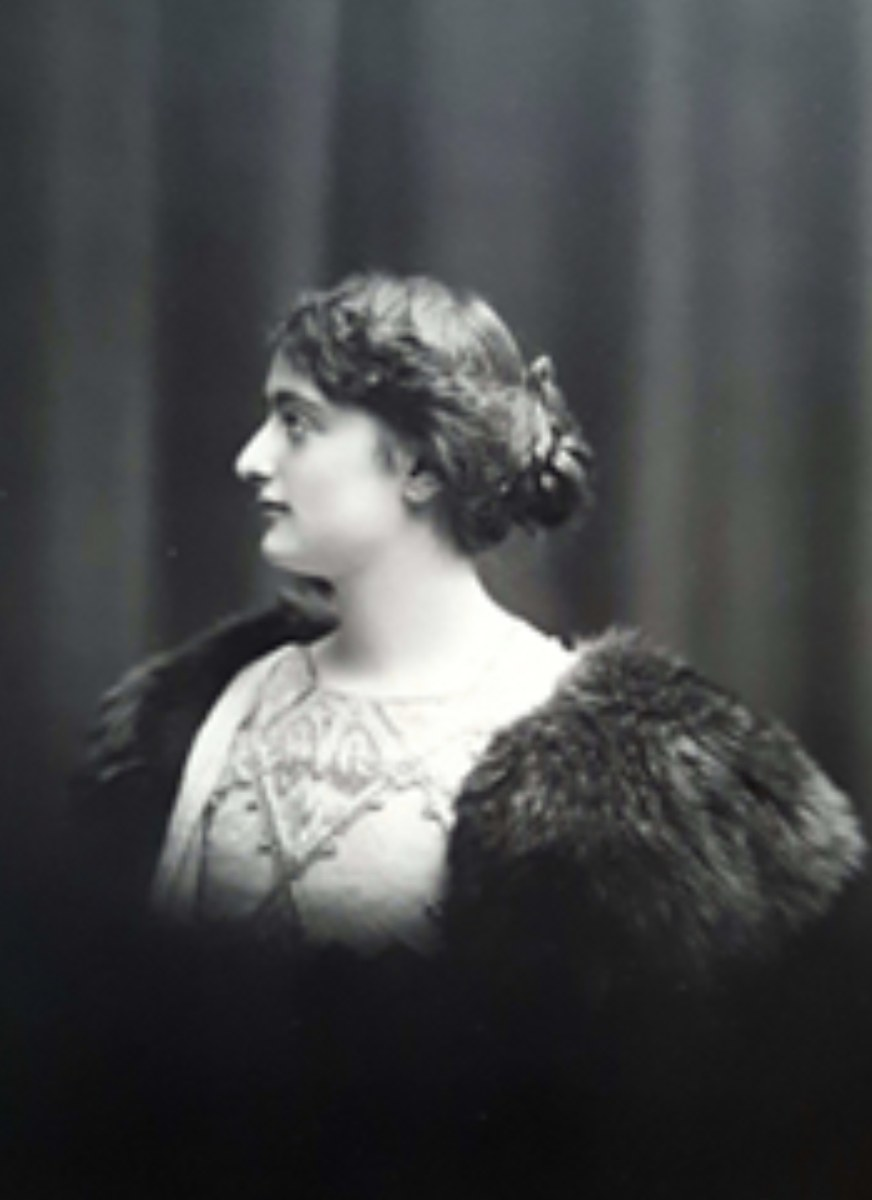
\includegraphics[width=0.94\linewidth,height=22mm,keepaspectratio]{illustrations/marguerite_1917.jpg}}
    \par\vspace{0.6mm}{\fontsize{5.8pt}{6.7pt}\selectfont Marguerite Calmels (1892--1974), photographiée par le studio Jublin à Millau à l'époque de ses fiançailles avec Hippolyte Combes.}
  \end{minipage}\hfill
  \begin{minipage}[b]{0.46\textwidth}
    \centering
    \setlength{\fboxsep}{0.7mm}\setlength{\fboxrule}{0.4pt}%
    \fcolorbox{gray!55}{white}{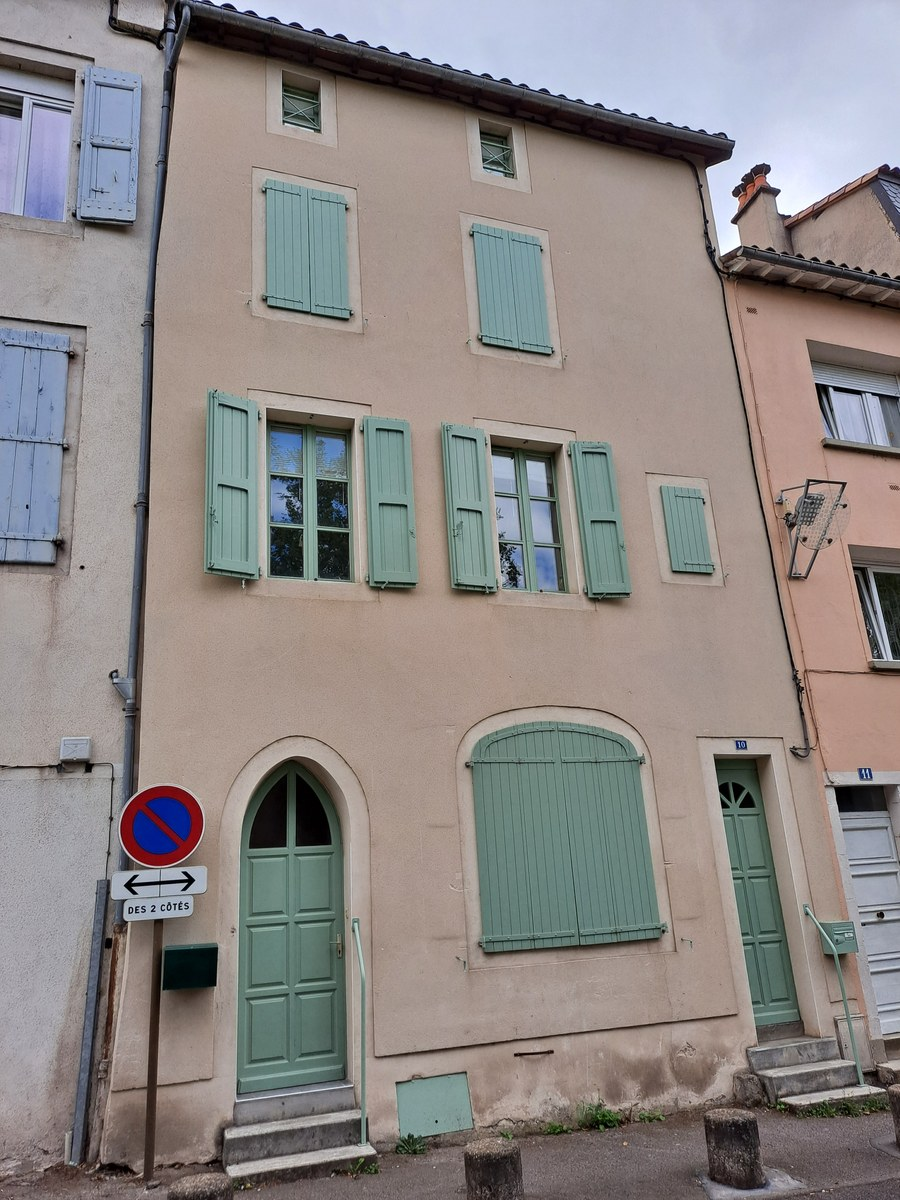
\includegraphics[width=0.94\linewidth,height=22mm,keepaspectratio]{illustrations/maison_millau.jpg}}
    \par\vspace{0.6mm}{\fontsize{5.8pt}{6.7pt}\selectfont La demeure familiale de Millau (Aveyron), berceau de la famille Combes.}
  \end{minipage}
\end{center}
\clearpage

% =============================================================================
% VIS-A-VIS SPREAD : SCAN #050 (20251126_103019.jpg) — Vue 050
% =============================================================================
\cleardoubleevenpage
% --- En-tête du folio (Page paire / gauche : Transcription, apparat & double registre) ---
\noindent\rule{\textwidth}{0.5pt}\par\vspace{0.6mm}
\noindent\textbf{\footnotesize SCAN \#050 — VUE 050} \hfill {\scriptsize\texttt{20251126\_\allowbreak 103019.jpg}}\par\vspace{0.3mm}
\noindent{\fontsize{7.0pt}{8.2pt}\selectfont Forceville et départ par Acheux-Varennes}\par\vspace{0.25mm}
\noindent{\fontsize{7.0pt}{8.2pt}\selectfont\textit{Lundi 25 septembre 1916 (matin et après-midi)} \hfill \textit{Forceville et gare d'Acheux-Varennes (Somme)}}\par\vspace{0.6mm}
\noindent\rule{\textwidth}{0.35pt}\par\vspace{1.0mm}
% --- Corps de la transcription diplomatique et apparat marginal en prolongement ---
{\renewcommand{\arraystretch}{1.02}%
\noindent\hspace*{3.5mm}\begin{tabular}{@{}p{100mm}@{\hspace{3.5mm}}p{55mm}@{}}
      \leavevmode\fontsize{7.8pt}{9.2pt}\selectfont\strut 25 L. \hfill{} Sept /16\strut & \leavevmode\fontsize{6.3pt}{7.2pt}\selectfont\raggedright\arraybackslash\color{black!88}\textbf{1} \textbf{L.} \textit{lundi} ; \textbf{Sept} \textit{septembre}. \\
      \leavevmode\fontsize{7.8pt}{9.2pt}\selectfont\strut Vers 7 H, sur pied.\strut &  \\
      \leavevmode\fontsize{7.8pt}{9.2pt}\selectfont\strut Au firmament bleuissant, léger croissant lunaire\strut &  \\
      \leavevmode\fontsize{7.8pt}{9.2pt}\selectfont\strut et 2 étoiles très brillantes.\strut &  \\
      \leavevmode\llap{\fontsize{6.5pt}{7.5pt}\selectfont\color{darkgray}5\hspace{1.8mm}}\fontsize{7.8pt}{9.2pt}\selectfont\strut Temps superbe.\strut &  \\
      \leavevmode\fontsize{7.8pt}{9.2pt}\selectfont\strut Bientôt, entiert prêt à partir.\strut & \leavevmode\fontsize{6.3pt}{7.2pt}\selectfont\raggedright\arraybackslash\color{black!88}\textbf{6} \textbf{entiert} \textit{entièrement}. \\
      \leavevmode\fontsize{7.8pt}{9.2pt}\selectfont\strut Promené champs tt en haut plateau.\strut & \leavevmode\fontsize{6.3pt}{7.2pt}\selectfont\raggedright\arraybackslash\color{black!88}\textbf{7} \textbf{tt} \textit{tout}. \\
      \leavevmode\fontsize{7.8pt}{9.2pt}\selectfont\strut Dû venir à Forceville av. Lt Ford, for green\strut & \leavevmode\fontsize{6.3pt}{7.2pt}\selectfont\raggedright\arraybackslash\color{black!88}\textbf{8} \textbf{av.} \textit{avec} ; \textbf{Lt} \textit{lieutenant} ; \textbf{for green} \textit{angl.} pour du fourrage vert ; forage continue à la ligne suivante. \\
      \leavevmode\fontsize{7.8pt}{9.2pt}\selectfont\strut forage. Chaleur très forte.\strut &  \\
      \leavevmode\llap{\fontsize{6.5pt}{7.5pt}\selectfont\color{darkgray}10\hspace{1.8mm}}\fontsize{7.8pt}{9.2pt}\selectfont\strut A midi enfin, monté sur le dernier wagon\strut &  \\
      \leavevmode\fontsize{7.8pt}{9.2pt}\selectfont\strut du convoy allant au railhead, puis continué\strut & \leavevmode\fontsize{6.3pt}{7.2pt}\selectfont\raggedright\arraybackslash\color{black!88}\textbf{11} \textbf{convoy} \textit{angl.} convoi ; \textbf{railhead} \textit{angl.} gare de ravitaillement en tête de ligne. \\
      \leavevmode\fontsize{7.8pt}{9.2pt}\selectfont\strut à travers chps j'à station d'Acheux-Varennes\strut & \leavevmode\fontsize{6.3pt}{7.2pt}\selectfont\raggedright\arraybackslash\color{black!88}\textbf{12} \textbf{chps} \textit{champs} ; \textbf{j'à} \textit{jusqu’à}. \\
      \leavevmode\fontsize{7.8pt}{9.2pt}\selectfont\strut Laissé mes colis à l'office de l'R.T.O. \& venu\strut & \leavevmode\fontsize{6.3pt}{7.2pt}\selectfont\raggedright\arraybackslash\color{black!88}\textbf{13} \textbf{office} \textit{angl.} bureau ; \textbf{R.T.O.} \textit{Railway Transport Officer : officier chargé des transports ferroviaires}. \\
      \leavevmode\fontsize{7.8pt}{9.2pt}\selectfont\strut village, déjeuné.\strut &  \\
      \leavevmode\llap{\fontsize{6.5pt}{7.5pt}\selectfont\color{darkgray}15\hspace{1.8mm}}\fontsize{7.8pt}{9.2pt}\selectfont\strut Puis attendu lgt. ds mon compartimt petit\strut & \leavevmode\fontsize{6.3pt}{7.2pt}\selectfont\raggedright\arraybackslash\color{black!88}\textbf{15} \textbf{lgt.} \textit{longtemps} ; \textbf{ds} \textit{dans} ; \textbf{compartimt} \textit{compartiment}. \\
      \leavevmode\fontsize{7.8pt}{9.2pt}\selectfont\strut train départemental en gare —\strut &  \\
      \leavevmode\fontsize{7.8pt}{9.2pt}\selectfont\strut chaleur intense\strut &  \\
      \leavevmode\fontsize{7.8pt}{9.2pt}\selectfont\strut [ Tip à mon groom : 2 f — Biscuits : 0.50 c\strut & \leavevmode\fontsize{6.3pt}{7.2pt}\selectfont\raggedright\arraybackslash\color{black!88}\textbf{18} \textbf{Tip} \textit{angl.} pourboire ; \textbf{groom} \textit{angl.} ordonnance ; soldat chargé ici du service personnel ; \textbf{Tip} Le compte est séparé du récit par un trait horizontal suivi d’un court retour vertical à gauche ; les crochets de la transcription sont éditoriaux. \\
      \leavevmode\fontsize{7.8pt}{9.2pt}\selectfont\strut Lunch à Acheux : 1 f 50 ]\strut & \leavevmode\fontsize{6.3pt}{7.2pt}\selectfont\raggedright\arraybackslash\color{black!88}\textbf{19} \textbf{Lunch} \textit{angl.} déjeuner. \\
\end{tabular}}%
\par\vspace*{\fill}
% --- Deux registres de commentaires en bas de page (sans intitulés, distingués par filets et mise en page) ---
\noindent\rule{\textwidth}{0.5pt}\par\vspace{0.8mm}
{\fontsize{6.8pt}{8.0pt}\selectfont%
\noindent\normalfont Le compte occupe le bas de la page, après un grand espace ; un trait horizontal et un retour vertical à gauche le distinguent du récit. Ce dispositif ne constitue pas une note marginale latérale. Les crochets imprimés ne sont pas transcrits comme des crochets autographes. Entiert, av. et compartimt sont développés. Le vocabulaire du ravitaillement et du voyage conserve ses formes anglaises, traduites localement.\par\vspace{0.75mm}
\noindent\rule{38mm}{0.4pt}\par\vspace{0.65mm}
\noindent\hspace*{5mm}\parbox{\dimexpr\textwidth-5mm\relax}{\fontsize{6.8pt}{8.0pt}\selectfont\color{black!82}\textbf{Départ en permission :} Le 25 septembre, Combes va à Forceville avec Lt Ford pour le fourrage, puis rejoint le railhead et la station d’Acheux-Varennes dans le dernier wagon du convoi. Il laisse ses colis à l’office R.T.O., puis attend dans un petit train départemental. La permission est confirmée au retour par son titre visé à Bernaville (vue 067). Cette entrée ne permet pas d’affirmer qu’il s’agit de sa toute première permission, ni de préciser l’écartement de la voie.}\par}
\newpage
% --- En-tête du fac-similé (Page impaire / droite : Scan original) ---
\noindent\rule{\textwidth}{0.5pt}\par\vspace{0.6mm}
\noindent\textbf{\fontsize{6.5pt}{7.6pt}\selectfont FAC-SIMILÉ EN VIS-À-VIS — VUE 050 (SCAN \#050)} \hfill {\fontsize{6.5pt}{7.6pt}\selectfont\texttt{20251126\_\allowbreak 103019.jpg}}\par\vspace{0.3mm}
\noindent{\fontsize{6.8pt}{8pt}\selectfont\textit{Livre-Journal d'Hippolyte Combes} — Lundi 25 septembre 1916 (matin et après-midi) (Forceville et gare d'Acheux-Varennes (Somme))}\par\vspace{0.6mm}
\noindent\rule{\textwidth}{0.35pt}\par\vspace*{\fill}
{\centering
  \setlength{\fboxsep}{1.2mm}%
  \setlength{\fboxrule}{0.4pt}%
  \fcolorbox{gray!55}{white}{%
    \includegraphics[width=0.94\textwidth,height=0.76\textheight,keepaspectratio]{\facsimiledir/20251126_103019.jpg}%
  }\par}
\vspace*{\fill}
\noindent\rule{\textwidth}{0.35pt}\par\vspace{0.5mm}
\noindent{\fontsize{6pt}{7.1pt}\selectfont\raggedright\color{darkgray}\textbf{Source :} Archives familiales Combes — Cliché numérique \texttt{20251126\_\allowbreak 103019.jpg} (Scan \#050/186, Vue 050). Haute définition : \texttt{scans\_haute\_qualite/\allowbreak 20251126\_\allowbreak 103019.jpg} ; version allégée : \texttt{scans\_compresses/\allowbreak 20251126\_\allowbreak 103019.jpg}.\par}
\newpage

% =============================================================================
% VIS-A-VIS SPREAD : SCAN #051 (20251126_103036.jpg) — Vue 051
% =============================================================================
\cleardoubleevenpage
% --- En-tête du folio (Page paire / gauche : Transcription, apparat & double registre) ---
\noindent\rule{\textwidth}{0.5pt}\par\vspace{0.6mm}
\noindent\textbf{\footnotesize SCAN \#051 — VUE 051} \hfill {\scriptsize\texttt{20251126\_\allowbreak 103036.jpg}}\par\vspace{0.3mm}
\noindent{\fontsize{7.0pt}{8.2pt}\selectfont Gézaincourt, Amiens et bombardement nocturne}\par\vspace{0.25mm}
\noindent{\fontsize{7.0pt}{8.2pt}\selectfont\textit{Lundi 25 septembre 1916 (soir et nuit)} \hfill \textit{Gézaincourt, Amiens, Longueau et train vers Paris}}\par\vspace{0.6mm}
\noindent\rule{\textwidth}{0.35pt}\par\vspace{1.0mm}
% --- Corps de la transcription diplomatique et apparat marginal en prolongement ---
{\renewcommand{\arraystretch}{1.02}%
\noindent\hspace*{3.5mm}\begin{tabular}{@{}p{100mm}@{\hspace{3.5mm}}p{55mm}@{}}
      \leavevmode\fontsize{7.8pt}{9.2pt}\selectfont\strut 25 Lundi. (Suite) \hfill{} Sept / 16\strut & \leavevmode\fontsize{6.3pt}{7.2pt}\selectfont\raggedright\arraybackslash\color{black!88}\textbf{1} \textbf{Sept} \textit{septembre}. \\
      \leavevmode\fontsize{7.8pt}{9.2pt}\selectfont\strut au ciel bleu, qq nuages, nettement détachés.\strut & \leavevmode\fontsize{6.3pt}{7.2pt}\selectfont\raggedright\arraybackslash\color{black!88}\textbf{2} \textbf{qq} \textit{quelques}. \\
      \leavevmode\fontsize{7.8pt}{9.2pt}\selectfont\strut Enfin, vers 3H 1/2, départ\strut &  \\
      \leavevmode\fontsize{7.8pt}{9.2pt}\selectfont\strut Doucement bercé par mouvement train. Et caresse\strut &  \\
      \leavevmode\llap{\fontsize{6.5pt}{7.5pt}\selectfont\color{darkgray}5\hspace{1.8mm}}\fontsize{7.8pt}{9.2pt}\selectfont\strut brise légère\strut &  \\
      \leavevmode\fontsize{7.8pt}{9.2pt}\selectfont\strut Verdures étincelantes de lumière. Bois ensoleillés.\strut &  \\
      \leavevmode\fontsize{7.8pt}{9.2pt}\selectfont\strut A Gézaincourt, vers 4H 1/2, changé train.\strut &  \\
      \leavevmode\fontsize{7.8pt}{9.2pt}\selectfont\strut Reparti à 5 H ds le train venant de Doullens\strut & \leavevmode\fontsize{6.3pt}{7.2pt}\selectfont\raggedright\arraybackslash\color{black!88}\textbf{8} \textbf{ds} \textit{dans}. \\
      \leavevmode\fontsize{7.8pt}{9.2pt}\selectfont\strut A Amiens, vers 8H s\strut &  \\
      \leavevmode\llap{\fontsize{6.5pt}{7.5pt}\selectfont\color{darkgray}10\hspace{1.8mm}}\fontsize{7.8pt}{9.2pt}\selectfont\strut Monté train de permissionns pr Paris. Compartimt\strut & \leavevmode\fontsize{6.3pt}{7.2pt}\selectfont\raggedright\arraybackslash\color{black!88}\textbf{10} \textbf{permissionns} \textit{permissionnaires} ; \textbf{pr} \textit{pour} ; \textbf{Compartimt} \textit{Compartiment}. \\
      \leavevmode\fontsize{7.8pt}{9.2pt}\selectfont\strut de 3e Cl., avec grossiers poilus, barbus \& sales\strut & \leavevmode\fontsize{6.3pt}{7.2pt}\selectfont\raggedright\arraybackslash\color{black!88}\textbf{11} \textbf{Cl.} \textit{classe}. \\
      \leavevmode\fontsize{7.8pt}{9.2pt}\selectfont\strut Roulé tte nuit\strut & \leavevmode\fontsize{6.3pt}{7.2pt}\selectfont\raggedright\arraybackslash\color{black!88}\textbf{12} \textbf{tte} \textit{toute}. \\
      \leavevmode\fontsize{7.8pt}{9.2pt}\selectfont\strut Après avoir quitté Amiens, et au croisement\strut &  \\
      \leavevmode\fontsize{7.8pt}{9.2pt}\selectfont\strut de Longueau, survolé par des Taubes qui\strut & \leavevmode\fontsize{6.3pt}{7.2pt}\selectfont\raggedright\arraybackslash\color{black!88}\textbf{14} \textbf{Taubes} \textit{all.} « colombes » en allemand ; désignation d’avions allemands. \\
      \leavevmode\llap{\fontsize{6.5pt}{7.5pt}\selectfont\color{darkgray}15\hspace{1.8mm}}\fontsize{7.8pt}{9.2pt}\selectfont\strut jeté bombes — obus ds les airs. Ciel fouillé\strut & \leavevmode\fontsize{6.3pt}{7.2pt}\selectfont\raggedright\arraybackslash\color{black!88}\textbf{15} \textbf{ds} \textit{dans} ; \textbf{jeté bombes} Construction elliptique du carnet ; ne pas transformer l’absence d’auxiliaire en abréviation ou lacune matérielle. \\
      \leavevmode\fontsize{7.8pt}{9.2pt}\selectfont\strut par les projecteurs. Très beau spectacle\strut &  \\
      \leavevmode\fontsize{7.8pt}{9.2pt}\selectfont\strut Pas descendu à Creil (en retard [?])\strut & \leavevmode\fontsize{6.3pt}{7.2pt}\selectfont\raggedright\arraybackslash\color{black!88}\textbf{17} \textbf{(en retard [?])} La fin de la parenthèse reste incertaine ; \textbf{Pas descendu à Creil} Les deux dernières lignes sont séparées du récit précédent par un grand blanc, sans être barrées. \\
      \leavevmode\fontsize{7.8pt}{9.2pt}\selectfont\strut Voyage tte la nuit\strut & \leavevmode\fontsize{6.3pt}{7.2pt}\selectfont\raggedright\arraybackslash\color{black!88}\textbf{18} \textbf{tte} \textit{toute}. \\
\end{tabular}}%
\par\vspace*{\fill}
% --- Deux registres de commentaires en bas de page (sans intitulés, distingués par filets et mise en page) ---
\noindent\rule{\textwidth}{0.5pt}\par\vspace{0.8mm}
{\fontsize{6.8pt}{8.0pt}\selectfont%
\noindent\normalfont Les deux dernières lignes sont portées au bas de la page après un blanc ; elles ne sont pas annulées. L’incertitude de la parenthèse après Creil demeure. Permissionns et compartimt sont des contractions omises dans les anciennes marges. Jeté bombes est une notation elliptique, sans lacune matérielle démontrée.\par\vspace{0.75mm}
\noindent\rule{38mm}{0.4pt}\par\vspace{0.65mm}
\noindent\hspace*{5mm}\parbox{\dimexpr\textwidth-5mm\relax}{\fontsize{6.8pt}{8.0pt}\selectfont\color{black!82}\textbf{Trajet vers Paris :} Après le changement de train à Gézaincourt, le récit donne Amiens vers 8 H du soir, puis le croisement de Longueau, des avions nommés Taubes, des bombes, des projecteurs et des obus dans les airs. Il décrit une attaque aérienne au cours du trajet sans permettre d’identifier le modèle exact des appareils. La parenthèse près de Creil demeure difficile et ne doit pas être développée par l’itinéraire supposé.}\par}
\newpage
% --- En-tête du fac-similé (Page impaire / droite : Scan original) ---
\noindent\rule{\textwidth}{0.5pt}\par\vspace{0.6mm}
\noindent\textbf{\fontsize{6.5pt}{7.6pt}\selectfont FAC-SIMILÉ EN VIS-À-VIS — VUE 051 (SCAN \#051)} \hfill {\fontsize{6.5pt}{7.6pt}\selectfont\texttt{20251126\_\allowbreak 103036.jpg}}\par\vspace{0.3mm}
\noindent{\fontsize{6.8pt}{8pt}\selectfont\textit{Livre-Journal d'Hippolyte Combes} — Lundi 25 septembre 1916 (soir et nuit) (Gézaincourt, Amiens, Longueau et train vers Paris)}\par\vspace{0.6mm}
\noindent\rule{\textwidth}{0.35pt}\par\vspace*{\fill}
{\centering
  \setlength{\fboxsep}{1.2mm}%
  \setlength{\fboxrule}{0.4pt}%
  \fcolorbox{gray!55}{white}{%
    \includegraphics[width=0.94\textwidth,height=0.76\textheight,keepaspectratio]{\facsimiledir/20251126_103036.jpg}%
  }\par}
\vspace*{\fill}
\noindent\rule{\textwidth}{0.35pt}\par\vspace{0.5mm}
\noindent{\fontsize{6pt}{7.1pt}\selectfont\raggedright\color{darkgray}\textbf{Source :} Archives familiales Combes — Cliché numérique \texttt{20251126\_\allowbreak 103036.jpg} (Scan \#051/186, Vue 051). Haute définition : \texttt{scans\_haute\_qualite/\allowbreak 20251126\_\allowbreak 103036.jpg} ; version allégée : \texttt{scans\_compresses/\allowbreak 20251126\_\allowbreak 103036.jpg}.\par}
\newpage

% =============================================================================
% VIS-A-VIS SPREAD : SCAN #052 (20251126_103109.jpg) — Vue 052
% =============================================================================
\cleardoubleevenpage
% --- En-tête du folio (Page paire / gauche : Transcription, apparat & double registre) ---
\noindent\rule{\textwidth}{0.5pt}\par\vspace{0.6mm}
\noindent\textbf{\footnotesize SCAN \#052 — VUE 052} \hfill {\scriptsize\texttt{20251126\_\allowbreak 103109.jpg}}\par\vspace{0.3mm}
\noindent{\fontsize{7.0pt}{8.2pt}\selectfont Du Bourget à Paris : démarches et courses}\par\vspace{0.25mm}
\noindent{\fontsize{7.0pt}{8.2pt}\selectfont\textit{Mardi 26 septembre 1916 (matin et après-midi)} \hfill \textit{Le Bourget et Paris (Gare du Nord, Tuileries, Orsay, Invalides, rive gauche)}}\par\vspace{0.6mm}
\noindent\rule{\textwidth}{0.35pt}\par\vspace{1.0mm}
% --- Corps de la transcription diplomatique et apparat marginal en prolongement ---
{\renewcommand{\arraystretch}{0.95}%
\noindent\hspace*{3.5mm}\begin{tabular}{@{}p{100mm}@{\hspace{3.5mm}}p{55mm}@{}}
      \leavevmode\fontsize{7.4pt}{8.6pt}\selectfont\strut Mardi 26 \hfill{} Sept 16\strut & \leavevmode\fontsize{6.3pt}{7.2pt}\selectfont\raggedright\arraybackslash\color{black!88}\textbf{1} \textbf{Sept} \textit{septembre}. \\
      \leavevmode\fontsize{7.4pt}{8.6pt}\selectfont\strut Vers 6H m., encore nuit, dû descendre gare\strut &  \\
      \leavevmode\fontsize{7.4pt}{8.6pt}\selectfont\strut du Bourget.\strut &  \\
      \leavevmode\fontsize{7.4pt}{8.6pt}\selectfont\strut Suivi voies j'que bureau militre. Là\strut & \leavevmode\fontsize{6.3pt}{7.2pt}\selectfont\raggedright\arraybackslash\color{black!88}\textbf{4} \textbf{j'que} \textit{jusque} ; \textbf{militre} \textit{militaire}. \\
      \leavevmode\llap{\fontsize{6.5pt}{7.5pt}\selectfont\color{darkgray}5\hspace{1.8mm}}\fontsize{7.4pt}{8.6pt}\selectfont\strut obtenu l'autorison de sortir et accompagné\strut & \leavevmode\fontsize{6.3pt}{7.2pt}\selectfont\raggedright\arraybackslash\color{black!88}\textbf{5} \textbf{autorison} \textit{autorisation}. \\
      \leavevmode\fontsize{7.4pt}{8.6pt}\selectfont\strut par un planton j'à la porte\strut & \leavevmode\fontsize{6.3pt}{7.2pt}\selectfont\raggedright\arraybackslash\color{black!88}\textbf{6} \textbf{j'à} \textit{jusqu’à}. \\
      \leavevmode\fontsize{7.4pt}{8.6pt}\selectfont\strut Du Bourget, sortie de la rue de Flandre\strut &  \\
      \leavevmode\fontsize{7.4pt}{8.6pt}\selectfont\strut pris tramway qui m'a conduit j-à gare\strut & \leavevmode\fontsize{6.3pt}{7.2pt}\selectfont\raggedright\arraybackslash\color{black!88}\textbf{8} \textbf{j-à} \textit{jusqu’à}. \\
      \leavevmode\fontsize{7.4pt}{8.6pt}\selectfont\strut du Nord. De là, par métro, arrivé\strut &  \\
      \leavevmode\llap{\fontsize{6.5pt}{7.5pt}\selectfont\color{darkgray}10\hspace{1.8mm}}\fontsize{7.4pt}{8.6pt}\selectfont\strut à Station Tuileries. (changé au Chatelet)\strut & \leavevmode\fontsize{6.3pt}{7.2pt}\selectfont\raggedright\arraybackslash\color{black!88}\textbf{10} \textbf{(changé au Chatelet)} Précision interlinéaire, placée à droite sous la mention de la station Tuileries. \\
      \leavevmode\fontsize{7.4pt}{8.6pt}\selectfont\strut Traversé jardin et\strut &  \\
      \leavevmode\fontsize{7.4pt}{8.6pt}\selectfont\strut Venu gare d'Orsay\strut &  \\
      \leavevmode\fontsize{7.4pt}{8.6pt}\selectfont\strut Me suis rendu à la Place (Hotel)\strut &  \\
      \leavevmode\fontsize{7.4pt}{8.6pt}\selectfont\strut des Invalides, pr demande autorison de\strut & \leavevmode\fontsize{6.3pt}{7.2pt}\selectfont\raggedright\arraybackslash\color{black!88}\textbf{14} \textbf{pr} \textit{pour} ; \textbf{autorison} \textit{autorisation}. \\
      \leavevmode\llap{\fontsize{6.5pt}{7.5pt}\selectfont\color{darkgray}15\hspace{1.8mm}}\fontsize{7.4pt}{8.6pt}\selectfont\strut voyager à mes frais en express. Revenu\strut &  \\
      \leavevmode\fontsize{7.4pt}{8.6pt}\selectfont\strut gare et pu enfin prendre billet de 2e cl.\strut & \leavevmode\fontsize{6.3pt}{7.2pt}\selectfont\raggedright\arraybackslash\color{black!88}\textbf{16} \textbf{cl.} \textit{classe}. \\
      \leavevmode\fontsize{7.4pt}{8.6pt}\selectfont\strut Toulouse\strut &  \\
      \leavevmode\fontsize{7.4pt}{8.6pt}\selectfont\strut Puis descendu rue du Bac\strut &  \\
      \leavevmode\fontsize{7.4pt}{8.6pt}\selectfont\strut Au Bon Marché\strut &  \\
      \leavevmode\llap{\fontsize{6.5pt}{7.5pt}\selectfont\color{darkgray}20\hspace{1.8mm}}\fontsize{7.4pt}{8.6pt}\selectfont\strut Rue de Rennes\strut &  \\
      \leavevmode\fontsize{7.4pt}{8.6pt}\selectfont\strut Jardin du Luxembourg\strut &  \\
      \leavevmode\fontsize{7.4pt}{8.6pt}\selectfont\strut Chez Colin\strut &  \\
\end{tabular}}%
\par\vspace*{\fill}
% --- Deux registres de commentaires en bas de page (sans intitulés, distingués par filets et mise en page) ---
\noindent\rule{\textwidth}{0.5pt}\par\vspace{0.8mm}
{\fontsize{6.8pt}{8.0pt}\selectfont%
\noindent\normalfont La parenthèse changé au Chatelet est une précision interlinéaire à droite, rattachée au trajet en métro. Les contractions de militaire et autorisation sont conservées sous leur forme manuscrite et développées en marge. Le passage à la ligne entre Place (Hotel) et des Invalides appartient au récit, sans rature assurée de ces mots.\par\vspace{0.75mm}
\noindent\rule{38mm}{0.4pt}\par\vspace{0.65mm}
\noindent\hspace*{5mm}\parbox{\dimexpr\textwidth-5mm\relax}{\fontsize{6.8pt}{8.0pt}\selectfont\color{black!82}\textbf{Paris :} Le 26 septembre, Combes obtient l’autorisation de sortir de la gare du Bourget, passe par la gare du Nord, les Tuileries et Orsay, puis demande aux Invalides à voyager à ses frais en express. Il note un billet de 2e classe pour Toulouse et termine par les commerces et promenades de la rive gauche. Le compte de la vue 053 porte séparément 1/4 place et 15 f 15. Le texte ne précise ni le bureau administratif exact aux Invalides ni l’adresse de Chez Colin.}\par}
\newpage
% --- En-tête du fac-similé (Page impaire / droite : Scan original) ---
\noindent\rule{\textwidth}{0.5pt}\par\vspace{0.6mm}
\noindent\textbf{\fontsize{6.5pt}{7.6pt}\selectfont FAC-SIMILÉ EN VIS-À-VIS — VUE 052 (SCAN \#052)} \hfill {\fontsize{6.5pt}{7.6pt}\selectfont\texttt{20251126\_\allowbreak 103109.jpg}}\par\vspace{0.3mm}
\noindent{\fontsize{6.8pt}{8pt}\selectfont\textit{Livre-Journal d'Hippolyte Combes} — Mardi 26 septembre 1916 (matin et après-midi) (Le Bourget et Paris (Gare du Nord, Tuileries, Orsay, Invalides, rive gauche))}\par\vspace{0.6mm}
\noindent\rule{\textwidth}{0.35pt}\par\vspace*{\fill}
{\centering
  \setlength{\fboxsep}{1.2mm}%
  \setlength{\fboxrule}{0.4pt}%
  \fcolorbox{gray!55}{white}{%
    \includegraphics[width=0.94\textwidth,height=0.76\textheight,keepaspectratio]{\facsimiledir/20251126_103109.jpg}%
  }\par}
\vspace*{\fill}
\noindent\rule{\textwidth}{0.35pt}\par\vspace{0.5mm}
\noindent{\fontsize{6pt}{7.1pt}\selectfont\raggedright\color{darkgray}\textbf{Source :} Archives familiales Combes — Cliché numérique \texttt{20251126\_\allowbreak 103109.jpg} (Scan \#052/186, Vue 052). Haute définition : \texttt{scans\_haute\_qualite/\allowbreak 20251126\_\allowbreak 103109.jpg} ; version allégée : \texttt{scans\_compresses/\allowbreak 20251126\_\allowbreak 103109.jpg}.\par}
\newpage

% =============================================================================
% VIS-A-VIS SPREAD : SCAN #053 (20251126_103131.jpg) — Vue 053
% =============================================================================
\cleardoubleevenpage
% --- En-tête du folio (Page paire / gauche : Transcription, apparat & double registre) ---
\noindent\rule{\textwidth}{0.5pt}\par\vspace{0.6mm}
\noindent\textbf{\footnotesize SCAN \#053 — VUE 053} \hfill {\scriptsize\texttt{20251126\_\allowbreak 103131.jpg}}\par\vspace{0.3mm}
\noindent{\fontsize{7.0pt}{8.2pt}\selectfont Paris : promenade, livres et dépenses}\par\vspace{0.25mm}
\noindent{\fontsize{7.0pt}{8.2pt}\selectfont\textit{Mardi 26 septembre 1916 (après-midi et soir)} \hfill \textit{Paris (Tour Saint-Jacques, rue de Rivoli, librairie Colin, gare d'Orsay)}}\par\vspace{0.6mm}
\noindent\rule{\textwidth}{0.35pt}\par\vspace{1.0mm}
% --- Corps de la transcription diplomatique et apparat marginal en prolongement ---
{\renewcommand{\arraystretch}{0.95}%
\noindent\hspace*{3.5mm}\begin{tabular}{@{}p{100mm}@{\hspace{3.5mm}}p{55mm}@{}}
      \leavevmode\fontsize{7.4pt}{8.6pt}\selectfont\strut Mardi 26 \hfill{} Sept 16\strut & \leavevmode\fontsize{6.3pt}{7.2pt}\selectfont\raggedright\arraybackslash\color{black!88}\textbf{1} \textbf{Sept} \textit{septembre}. \\
      \leavevmode\fontsize{7.4pt}{8.6pt}\selectfont\strut Déjeuné – Bd St-Germain\strut & \leavevmode\fontsize{6.3pt}{7.2pt}\selectfont\raggedright\arraybackslash\color{black!88}\textbf{2} \textbf{Bd} \textit{boulevard} ; \textbf{St} \textit{Saint}. \\
      \leavevmode\fontsize{7.4pt}{8.6pt}\selectfont\strut Reposé – jardin Notre - Dame\strut &  \\
      \leavevmode\fontsize{7.4pt}{8.6pt}\selectfont\strut Magasins de l'Hotel - de - Ville\strut &  \\
      \leavevmode\llap{\fontsize{6.5pt}{7.5pt}\selectfont\color{darkgray}5\hspace{1.8mm}}\fontsize{7.4pt}{8.6pt}\selectfont\strut [Lgt/1/2 h ?] assis banc ds le square de la\strut & \leavevmode\fontsize{6.3pt}{7.2pt}\selectfont\raggedright\arraybackslash\color{black!88}\textbf{5} \textbf{[Lgt/1/2 h ?]} La durée ou l’adverbe avant assis reste indécidable ; ne pas développer longtemps comme une leçon certaine ; \textbf{ds} \textit{dans}. \\
      \leavevmode\fontsize{7.4pt}{8.6pt}\selectfont\strut Tour St-Jacques — Gros mouvt de rue de\strut & \leavevmode\fontsize{6.3pt}{7.2pt}\selectfont\raggedright\arraybackslash\color{black!88}\textbf{6} \textbf{St} \textit{Saint} ; \textbf{mouvt} \textit{mouvement}. \\
      \leavevmode\fontsize{7.4pt}{8.6pt}\selectfont\strut Rivoli. Animation ordinre. —\strut & \leavevmode\fontsize{6.3pt}{7.2pt}\selectfont\raggedright\arraybackslash\color{black!88}\textbf{7} \textbf{ordinre} \textit{ordinaire}. \\
      \leavevmode\fontsize{7.4pt}{8.6pt}\selectfont\strut Après diner, venu lentemt, par les\strut & \leavevmode\fontsize{6.3pt}{7.2pt}\selectfont\raggedright\arraybackslash\color{black!88}\textbf{8} \textbf{lentemt} \textit{lentement}. \\
      \leavevmode\fontsize{7.4pt}{8.6pt}\selectfont\strut quais à gare d'Orsay\strut &  \\
      \leavevmode\llap{\fontsize{6.5pt}{7.5pt}\selectfont\color{darkgray}10\hspace{1.8mm}}\fontsize{7.4pt}{8.6pt}\selectfont\strut Départ train vers 8H S\strut &  \\
      \leavevmode\fontsize{7.4pt}{8.6pt}\selectfont\strut Tramway : Bourget - gare du Nord : 50c\strut & \leavevmode\fontsize{6.3pt}{7.2pt}\selectfont\raggedright\arraybackslash\color{black!88}\textbf{11} \textbf{Tramway} Les dépenses commencent sous un trait horizontal qui traverse la page ; elles ne sont pas une addition en marge latérale. \\
      \leavevmode\fontsize{7.4pt}{8.6pt}\selectfont\strut Métro : 1 f. — Envoi[s?] : 10 c, 1 f, 2 f. ([mot incertain])\strut & \leavevmode\fontsize{6.3pt}{7.2pt}\selectfont\raggedright\arraybackslash\color{black!88}\textbf{12} \textbf{Envoi[s?]} Intitulé proposé ; finale incertaine ; \textbf{[mot incertain]} Le mot parenthétique n’est pas établi. \\
      \leavevmode\fontsize{7.4pt}{8.6pt}\selectfont\strut Billet 2e cl. Toulouse 1/4 place : 15 f 15 \hfill{} Coupe chvx : 1 f\strut & \leavevmode\fontsize{6.3pt}{7.2pt}\selectfont\raggedright\arraybackslash\color{black!88}\textbf{13} \textbf{cl.} \textit{classe} ; \textbf{chvx} \textit{cheveux}. \\
      \leavevmode\fontsize{7.4pt}{8.6pt}\selectfont\strut Christofle : 12 f 50, remise, une [mot illis.] : 10 f 50\strut & \leavevmode\fontsize{6.3pt}{7.2pt}\selectfont\raggedright\arraybackslash\color{black!88}\textbf{14} \textbf{[mot illis.]} L’objet de la réduction Christofle n’est pas identifié. \\
      \leavevmode\llap{\fontsize{6.5pt}{7.5pt}\selectfont\color{darkgray}15\hspace{1.8mm}}\fontsize{7.4pt}{8.6pt}\selectfont\strut Zyromski : L'orgueil humain : 4 f : net : 3 f 20\strut &  \\
      \leavevmode\fontsize{7.4pt}{8.6pt}\selectfont\strut Maeterlinck : Les Débris : 3 f 50. — Cirage : 25 c\strut &  \\
      \leavevmode\fontsize{7.4pt}{8.6pt}\selectfont\strut Déjeuner : 1 f 50. — Dîner : 1 f 60. — Ctes ples : 15 c\strut & \leavevmode\fontsize{6.3pt}{7.2pt}\selectfont\raggedright\arraybackslash\color{black!88}\textbf{17} \textbf{Ctes ples} \textit{cartes postales}. \\
      \leavevmode\fontsize{7.4pt}{8.6pt}\selectfont\strut Fleurs artiflles, Hotel de Ville : 8 f 50 couronne\strut & \leavevmode\fontsize{6.3pt}{7.2pt}\selectfont\raggedright\arraybackslash\color{black!88}\textbf{18} \textbf{artiflles} \textit{artificielles}. \\
      \leavevmode\fontsize{7.4pt}{8.6pt}\selectfont\strut Képi : au Bon Marché : 8 f 75. — Consigne : 15 c\strut &  \\
      \leavevmode\llap{\fontsize{6.5pt}{7.5pt}\selectfont\color{darkgray}20\hspace{1.8mm}}\fontsize{7.4pt}{8.6pt}\selectfont\strut Carte de Verdun : 50 c — [Entretien ?] souliers : 30 c\strut & \leavevmode\fontsize{6.3pt}{7.2pt}\selectfont\raggedright\arraybackslash\color{black!88}\textbf{20} \textbf{[Entretien ?]} Lecture proposée du poste concernant les souliers. \\
      \leavevmode\fontsize{7.4pt}{8.6pt}\selectfont\strut Carte Roumanie : 30 c — [Divers ?] : W.C. : [15 c ?]\strut & \leavevmode\fontsize{6.3pt}{7.2pt}\selectfont\raggedright\arraybackslash\color{black!88}\textbf{21} \textbf{[Divers ?]} Intitulé final proposé, sans certitude ; \textbf{W.C.} \textit{water-closet : toilettes} ; \textbf{[15 c ?]} Montant final réservé. \\
\end{tabular}}%
\par\vspace*{\fill}
% --- Deux registres de commentaires en bas de page (sans intitulés, distingués par filets et mise en page) ---
\noindent\rule{\textwidth}{0.5pt}\par\vspace{0.8mm}
{\fontsize{6.8pt}{8.0pt}\selectfont%
\noindent\normalfont Un trait horizontal sépare le récit des dépenses, disposées en lignes avec plusieurs postes sur la même ligne. La durée près du square, le mot parenthétique après les envois et l’objet acheté chez Christofle restent non établis. Entretien et Divers sont des propositions ; les signes de réserve ne désignent ni des mots effacés ni des lacunes du support. Les contractions de mouvement, ordinaire, lentement, cheveux et cartes postales sont développées à leur ligne.\par\vspace{0.75mm}
\noindent\rule{38mm}{0.4pt}\par\vspace{0.65mm}
\noindent\hspace*{5mm}\parbox{\dimexpr\textwidth-5mm\relax}{\fontsize{6.8pt}{8.0pt}\selectfont\color{black!82}\textbf{Livres et achats :} Les formes Zyromski, L’orgueil humain et Maeterlinck, Les Débris se rapprochent de deux titres documentés : Ernest Zyromski, L’Orgueil humain (Armand Colin, 1904 ; compte rendu de Maurice Souriau, 1907, p. 81–83) et Maurice Maeterlinck, Les Débris de la guerre (Fasquelle, 1916 ; catalogue du Musée Arnold vander Haeghen). Cette identification bibliographique ne restitue pas les mots omis dans le carnet. Les prix 4 f/net 3 f 20 et 3 f 50, la couronne de fleurs artificielles et le képi figurent au compte ; le destinataire de la couronne n’est pas indiqué ici. La vue 057 ne mentionne pas de dépôt de couronne.}\par}
\newpage
% --- En-tête du fac-similé (Page impaire / droite : Scan original) ---
\noindent\rule{\textwidth}{0.5pt}\par\vspace{0.6mm}
\noindent\textbf{\fontsize{6.5pt}{7.6pt}\selectfont FAC-SIMILÉ EN VIS-À-VIS — VUE 053 (SCAN \#053)} \hfill {\fontsize{6.5pt}{7.6pt}\selectfont\texttt{20251126\_\allowbreak 103131.jpg}}\par\vspace{0.3mm}
\noindent{\fontsize{6.8pt}{8pt}\selectfont\textit{Livre-Journal d'Hippolyte Combes} — Mardi 26 septembre 1916 (après-midi et soir) (Paris (Tour Saint-Jacques, rue de Rivoli, librairie Colin, gare d'Orsay))}\par\vspace{0.6mm}
\noindent\rule{\textwidth}{0.35pt}\par\vspace*{\fill}
{\centering
  \setlength{\fboxsep}{1.2mm}%
  \setlength{\fboxrule}{0.4pt}%
  \fcolorbox{gray!55}{white}{%
    \includegraphics[width=0.94\textwidth,height=0.76\textheight,keepaspectratio]{\facsimiledir/20251126_103131.jpg}%
  }\par}
\vspace*{\fill}
\noindent\rule{\textwidth}{0.35pt}\par\vspace{0.5mm}
\noindent{\fontsize{6pt}{7.1pt}\selectfont\raggedright\color{darkgray}\textbf{Source :} Archives familiales Combes — Cliché numérique \texttt{20251126\_\allowbreak 103131.jpg} (Scan \#053/186, Vue 053). Haute définition : \texttt{scans\_haute\_qualite/\allowbreak 20251126\_\allowbreak 103131.jpg} ; version allégée : \texttt{scans\_compresses/\allowbreak 20251126\_\allowbreak 103131.jpg}.\par}
\newpage

% =============================================================================
% VIS-A-VIS SPREAD : SCAN #054 (20251126_103146.jpg) — Vue 054
% =============================================================================
\cleardoubleevenpage
% --- En-tête du folio (Page paire / gauche : Transcription, apparat & double registre) ---
\noindent\rule{\textwidth}{0.5pt}\par\vspace{0.6mm}
\noindent\textbf{\footnotesize SCAN \#054 — VUE 054} \hfill {\scriptsize\texttt{20251126\_\allowbreak 103146.jpg}}\par\vspace{0.3mm}
\noindent{\fontsize{7.0pt}{8.2pt}\selectfont Arrivée à Toulouse et retrouvailles}\par\vspace{0.25mm}
\noindent{\fontsize{7.0pt}{8.2pt}\selectfont\textit{Mercredi 27 septembre 1916} \hfill \textit{Toulouse (Sainte-Marie-des-Champs)}}\par\vspace{0.6mm}
\noindent\rule{\textwidth}{0.35pt}\par\vspace{1.0mm}
% --- Corps de la transcription diplomatique et apparat marginal en prolongement ---
{\renewcommand{\arraystretch}{1.02}%
\noindent\hspace*{3.5mm}\begin{tabular}{@{}p{100mm}@{\hspace{3.5mm}}p{55mm}@{}}
      \leavevmode\fontsize{7.8pt}{9.2pt}\selectfont\strut 27 Mer. \hfill{} Sept 1916\strut & \leavevmode\fontsize{6.3pt}{7.2pt}\selectfont\raggedright\arraybackslash\color{black!88}\textbf{1} \textbf{Mer.} \textit{mercredi} ; \textbf{Sept} \textit{septembre}. \\
      \leavevmode\fontsize{7.8pt}{9.2pt}\selectfont\strut Nuit passée ds [wagt ?]. Dormi 1 peu\strut & \leavevmode\fontsize{6.3pt}{7.2pt}\selectfont\raggedright\arraybackslash\color{black!88}\textbf{2} \textbf{ds} \textit{dans} ; \textbf{[wagt ?]} Le groupe commence par wa- et possède une descendante ; wagon est proposé, mais la finale abrégée reste incertaine. Compmt n’est pas soutenu par le cliché. \\
      \leavevmode\fontsize{7.8pt}{9.2pt}\selectfont\strut A 7H 30 m., arrivé à Toulouse\strut &  \\
      \leavevmode\fontsize{7.8pt}{9.2pt}\selectfont\strut Pris tram et vers 8H, ds mon appartement\strut & \leavevmode\fontsize{6.3pt}{7.2pt}\selectfont\raggedright\arraybackslash\color{black!88}\textbf{4} \textbf{ds} \textit{dans}. \\
      \leavevmode\llap{\fontsize{6.5pt}{7.5pt}\selectfont\color{darkgray}5\hspace{1.8mm}}\fontsize{7.8pt}{9.2pt}\selectfont\strut A 11 H m. — monté à Ste Marie-des-Champs. Les dames\strut & \leavevmode\fontsize{6.3pt}{7.2pt}\selectfont\raggedright\arraybackslash\color{black!88}\textbf{5} \textbf{Ste} \textit{Sainte}. \\
      \leavevmode\fontsize{7.8pt}{9.2pt}\selectfont\strut Calmels, pas e. arrivées, ne seront là que ce soir —\strut & \leavevmode\fontsize{6.3pt}{7.2pt}\selectfont\raggedright\arraybackslash\color{black!88}\textbf{6} \textbf{e.} \textit{encore}. \\
      \leavevmode\fontsize{7.8pt}{9.2pt}\selectfont\strut Déjeuné chz les Crouzet, ds la + gde intimité —\strut & \leavevmode\fontsize{6.3pt}{7.2pt}\selectfont\raggedright\arraybackslash\color{black!88}\textbf{7} \textbf{chz} \textit{chez} ; \textbf{ds} \textit{dans} ; \textbf{gde} \textit{grande}. \\
      \leavevmode\fontsize{7.8pt}{9.2pt}\selectfont\strut Redescendu après-midi en ville et fait courses\strut &  \\
      \leavevmode\fontsize{7.8pt}{9.2pt}\selectfont\strut diverses\strut &  \\
      \leavevmode\llap{\fontsize{6.5pt}{7.5pt}\selectfont\color{darkgray}10\hspace{1.8mm}}\fontsize{7.8pt}{9.2pt}\selectfont\strut A 5H, remonté Cote Pavée. Enfin, revu\strut &  \\
      \leavevmode\fontsize{7.8pt}{9.2pt}\selectfont\strut Margte. Charmante de simplicité \& de tendresse\strut & \leavevmode\fontsize{6.3pt}{7.2pt}\selectfont\raggedright\arraybackslash\color{black!88}\textbf{11} \textbf{Margte} \textit{Marguerite}. \\
      \leavevmode\fontsize{7.8pt}{9.2pt}\selectfont\strut confiante.\strut &  \\
      \leavevmode\fontsize{7.8pt}{9.2pt}\selectfont\strut Trams : 10, 10, 20 c..\strut & \leavevmode\fontsize{6.3pt}{7.2pt}\selectfont\raggedright\arraybackslash\color{black!88}\textbf{13} \textbf{Trams} Les dépenses sont placées au bas de la page sous un trait horizontal, après un grand blanc. \\
      \leavevmode\fontsize{7.8pt}{9.2pt}\selectfont\strut Bain, aux Thermes du Languedoc : 90 c + [15 c / 1 f ?]\strut & \leavevmode\fontsize{6.3pt}{7.2pt}\selectfont\raggedright\arraybackslash\color{black!88}\textbf{14} \textbf{[15 c / 1 f ?]} Le petit montant ajouté après le prix du bain reste difficile à distinguer. \\
      \leavevmode\llap{\fontsize{6.5pt}{7.5pt}\selectfont\color{darkgray}15\hspace{1.8mm}}\fontsize{7.8pt}{9.2pt}\selectfont\strut Cartes ples :\strut & \leavevmode\fontsize{6.3pt}{7.2pt}\selectfont\raggedright\arraybackslash\color{black!88}\textbf{15} \textbf{ples} \textit{postales}. \\
\end{tabular}}%
\par\vspace*{\fill}
% --- Deux registres de commentaires en bas de page (sans intitulés, distingués par filets et mise en page) ---
\noindent\rule{\textwidth}{0.5pt}\par\vspace{0.8mm}
{\fontsize{6.8pt}{8.0pt}\selectfont%
\noindent\normalfont La première ligne du récit ne porte pas compmt : le groupe abrégé après ds présente wa- et une descendante. La proposition wagt, à développer prudemment par wagon, est conservée avec réserve. Pas e. signifie pas encore ; chz et gde sont des contractions omises ou incomplètement expliquées. Les comptes sont séparés du récit par un trait inférieur. Le supplément ajouté au bain reste incertain.\par\vspace{0.75mm}
\noindent\rule{38mm}{0.4pt}\par\vspace{0.65mm}
\noindent\hspace*{5mm}\parbox{\dimexpr\textwidth-5mm\relax}{\fontsize{6.8pt}{8.0pt}\selectfont\color{black!82}\textbf{Famille à Toulouse :} Combes retrouve les dames Calmels, les Crouzet et Margte. L’acte de naissance de Marguerite Calmels (1892, n°117) nomme ses parents Gabriel Calmels, médecin, et Valentine Cartairade ; Émile Crouzet, agent de change à Toulouse, y est témoin. La section Les Crouzet de l’annexe familiale de Pierre Combes présente Émile Crouzet (1842–1921), son épouse Élisabeth Calmels et Jean Crouzet. Ces pièces éclairent le réseau familial ; l’identification de chaque désignation abrégée du carnet doit garder son degré propre de vraisemblance.}\par}
\newpage
% --- En-tête du fac-similé (Page impaire / droite : Scan original) ---
\noindent\rule{\textwidth}{0.5pt}\par\vspace{0.6mm}
\noindent\textbf{\fontsize{6.5pt}{7.6pt}\selectfont FAC-SIMILÉ EN VIS-À-VIS — VUE 054 (SCAN \#054)} \hfill {\fontsize{6.5pt}{7.6pt}\selectfont\texttt{20251126\_\allowbreak 103146.jpg}}\par\vspace{0.3mm}
\noindent{\fontsize{6.8pt}{8pt}\selectfont\textit{Livre-Journal d'Hippolyte Combes} — Mercredi 27 septembre 1916 (Toulouse (Sainte-Marie-des-Champs))}\par\vspace{0.6mm}
\noindent\rule{\textwidth}{0.35pt}\par\vspace*{\fill}
{\centering
  \setlength{\fboxsep}{1.2mm}%
  \setlength{\fboxrule}{0.4pt}%
  \fcolorbox{gray!55}{white}{%
    \includegraphics[width=0.94\textwidth,height=0.76\textheight,keepaspectratio]{\facsimiledir/20251126_103146.jpg}%
  }\par}
\vspace*{\fill}
\noindent\rule{\textwidth}{0.35pt}\par\vspace{0.5mm}
\noindent{\fontsize{6pt}{7.1pt}\selectfont\raggedright\color{darkgray}\textbf{Source :} Archives familiales Combes — Cliché numérique \texttt{20251126\_\allowbreak 103146.jpg} (Scan \#054/186, Vue 054). Haute définition : \texttt{scans\_haute\_qualite/\allowbreak 20251126\_\allowbreak 103146.jpg} ; version allégée : \texttt{scans\_compresses/\allowbreak 20251126\_\allowbreak 103146.jpg}.\par}
\newpage

% =============================================================================
% VIS-A-VIS SPREAD : SCAN #055 (20251126_103215.jpg) — Vue 055
% =============================================================================
\cleardoubleevenpage
% --- En-tête du folio (Page paire / gauche : Transcription, apparat & double registre) ---
\noindent\rule{\textwidth}{0.5pt}\par\vspace{0.6mm}
\noindent\textbf{\footnotesize SCAN \#055 — VUE 055} \hfill {\scriptsize\texttt{20251126\_\allowbreak 103215.jpg}}\par\vspace{0.3mm}
\noindent{\fontsize{7.0pt}{8.2pt}\selectfont Souvenirs et promenade vers Pech-David}\par\vspace{0.25mm}
\noindent{\fontsize{7.0pt}{8.2pt}\selectfont\textit{Jeudi 28 septembre 1916} \hfill \textit{Toulouse (Sainte-Marie, barrière Saint-Agne, Pouvourville, Pech-David)}}\par\vspace{0.6mm}
\noindent\rule{\textwidth}{0.35pt}\par\vspace{1.0mm}
% --- Corps de la transcription diplomatique et apparat marginal en prolongement ---
{\renewcommand{\arraystretch}{0.95}%
\noindent\hspace*{3.5mm}\begin{tabular}{@{}p{100mm}@{\hspace{3.5mm}}p{55mm}@{}}
      \leavevmode\fontsize{7.4pt}{8.6pt}\selectfont\strut 28 Jeudi. \hfill{} Sept 16\strut & \leavevmode\fontsize{6.3pt}{7.2pt}\selectfont\raggedright\arraybackslash\color{black!88}\textbf{1} \textbf{Sept} \textit{septembre}. \\
      \leavevmode\fontsize{7.4pt}{8.6pt}\selectfont\strut Me suis attardé ds mon appartt — Pris un\strut & \leavevmode\fontsize{6.3pt}{7.2pt}\selectfont\raggedright\arraybackslash\color{black!88}\textbf{2} \textbf{ds} \textit{dans} ; \textbf{appartt} \textit{appartement}. \\
      \leavevmode\fontsize{7.4pt}{8.6pt}\selectfont\strut plaisir extrême à regarder \& ranger mes\strut &  \\
      \leavevmode\fontsize{7.4pt}{8.6pt}\selectfont\strut affaires, et à laisser peu à peu\strut &  \\
      \leavevmode\llap{\fontsize{6.5pt}{7.5pt}\selectfont\color{darkgray}5\hspace{1.8mm}}\fontsize{7.4pt}{8.6pt}\selectfont\strut s'éveiller p moi des souvenirs du passé.\strut & \leavevmode\fontsize{6.3pt}{7.2pt}\selectfont\raggedright\arraybackslash\color{black!88}\textbf{5} \textbf{p moi} Le petit signe avant moi reste ambigu : le développement pour n’est pas garanti par le contexte. \\
      \leavevmode\fontsize{7.4pt}{8.6pt}\selectfont\strut Monté à Ste-Marie, vers 11 H 1/2. Apporté à Mte\strut & \leavevmode\fontsize{6.3pt}{7.2pt}\selectfont\raggedright\arraybackslash\color{black!88}\textbf{6} \textbf{Ste} \textit{Sainte} ; \textbf{Mte} \textit{Marguerite}. \\
      \leavevmode\fontsize{7.4pt}{8.6pt}\selectfont\strut un très joli bouquet fleurs délicates.\strut &  \\
      \leavevmode\fontsize{7.4pt}{8.6pt}\selectfont\strut Mêmes impressions au sujet de ma fiancée :\strut &  \\
      \leavevmode\fontsize{7.4pt}{8.6pt}\selectfont\strut tjs simple, affectueuse, charmante\strut & \leavevmode\fontsize{6.3pt}{7.2pt}\selectfont\raggedright\arraybackslash\color{black!88}\textbf{9} \textbf{tjs} \textit{toujours}. \\
      \leavevmode\llap{\fontsize{6.5pt}{7.5pt}\selectfont\color{darkgray}10\hspace{1.8mm}}\fontsize{7.4pt}{8.6pt}\selectfont\strut Après déjeun., promenade en cie Mme C. et\strut & \leavevmode\fontsize{6.3pt}{7.2pt}\selectfont\raggedright\arraybackslash\color{black!88}\textbf{10} \textbf{déjeun.} \textit{déjeuner} ; \textbf{cie} \textit{compagnie} ; \textbf{Mme} \textit{Madame}. \\
      \leavevmode\fontsize{7.4pt}{8.6pt}\selectfont\strut M. Czt. Descendu à pied côte vers St Joseph et\strut & \leavevmode\fontsize{6.3pt}{7.2pt}\selectfont\raggedright\arraybackslash\color{black!88}\textbf{11} \textbf{M.} \textit{Monsieur} ; \textbf{Czt.} \textit{Crouzet, contraction du patronyme} ; \textbf{St} \textit{Saint}. \\
      \leavevmode\fontsize{7.4pt}{8.6pt}\selectfont\strut arrivé j'à la barrière St-Agne. De là, pris trams\strut & \leavevmode\fontsize{6.3pt}{7.2pt}\selectfont\raggedright\arraybackslash\color{black!88}\textbf{12} \textbf{j'à} \textit{jusqu’à} ; \textbf{St} \textit{Saint}. \\
      \leavevmode\fontsize{7.4pt}{8.6pt}\selectfont\strut j-à St-Agne. Remonté par route ombragée\strut & \leavevmode\fontsize{6.3pt}{7.2pt}\selectfont\raggedright\arraybackslash\color{black!88}\textbf{13} \textbf{j-à} \textit{jusqu’à} ; \textbf{St} \textit{Saint}. \\
      \leavevmode\fontsize{7.4pt}{8.6pt}\selectfont\strut j'au village de Pouvourville, église —\strut & \leavevmode\fontsize{6.3pt}{7.2pt}\selectfont\raggedright\arraybackslash\color{black!88}\textbf{14} \textbf{j'au} \textit{jusqu’au}. \\
      \leavevmode\llap{\fontsize{6.5pt}{7.5pt}\selectfont\color{darkgray}15\hspace{1.8mm}}\fontsize{7.4pt}{8.6pt}\selectfont\strut Puis, sur la hauteur, d'où vue superbe\strut &  \\
      \leavevmode\fontsize{7.4pt}{8.6pt}\selectfont\strut suivi crête de Pech David — j'au carref.\strut & \leavevmode\fontsize{6.3pt}{7.2pt}\selectfont\raggedright\arraybackslash\color{black!88}\textbf{16} \textbf{j'au} \textit{jusqu’au} ; \textbf{carref.} \textit{carrefour}. \\
      \leavevmode\fontsize{7.4pt}{8.6pt}\selectfont\strut Récollets et Caserne\strut &  \\
      \leavevmode\fontsize{7.4pt}{8.6pt}\selectfont\strut Allé prendre trams à la barrière St-Agne\strut & \leavevmode\fontsize{6.3pt}{7.2pt}\selectfont\raggedright\arraybackslash\color{black!88}\textbf{18} \textbf{St} \textit{Saint}. \\
      \leavevmode\fontsize{7.4pt}{8.6pt}\selectfont\strut Exc.te après-midi.\strut & \leavevmode\fontsize{6.3pt}{7.2pt}\selectfont\raggedright\arraybackslash\color{black!88}\textbf{19} \textbf{Exc.te} \textit{Excellente}. \\
      \leavevmode\llap{\fontsize{6.5pt}{7.5pt}\selectfont\color{darkgray}20\hspace{1.8mm}}\fontsize{7.4pt}{8.6pt}\selectfont\strut Vers 9 H 30 s, redescendu à pied Cote Pavée\strut &  \\
      \leavevmode\fontsize{7.4pt}{8.6pt}\selectfont\strut Trams : 20 c, 40, 40, 40 c. —\strut &  \\
      \leavevmode\fontsize{7.4pt}{8.6pt}\selectfont\strut Fruits (raisins \& grenades) : 1 f — Varia : 10 c.\strut & \leavevmode\fontsize{6.3pt}{7.2pt}\selectfont\raggedright\arraybackslash\color{black!88}\textbf{22} \textbf{Varia} \textit{lat.} divers ; rubrique de petites dépenses. \\
      \leavevmode\fontsize{7.4pt}{8.6pt}\selectfont\strut Bouquet (place Esquirol) : 3 f —\strut &  \\
\end{tabular}}%
\par\vspace*{\fill}
% --- Deux registres de commentaires en bas de page (sans intitulés, distingués par filets et mise en page) ---
\noindent\rule{\textwidth}{0.5pt}\par\vspace{0.8mm}
{\fontsize{6.8pt}{8.0pt}\selectfont%
\noindent\normalfont Le compte suit immédiatement un trait horizontal tracé sous la dernière ligne du récit. Les montants des trams et des fruits sont conservés. Déjeun. est ici le substantif déjeuner après Après. Le groupe cie, le carref. et Exc.te sont des contractions lexicales, non des lectures lacunaires. Le petit signe p avant moi reste sans développement certain.\par\vspace{0.75mm}
\noindent\rule{38mm}{0.4pt}\par\vspace{0.65mm}
\noindent\hspace*{5mm}\parbox{\dimexpr\textwidth-5mm\relax}{\fontsize{6.8pt}{8.0pt}\selectfont\color{black!82}\textbf{Promenade toulousaine :} Le bouquet offert à Margte est compté place Esquirol. La promenade associe Mme C., M. Czt., Saint-Agne, Pouvourville, Pech David et les Récollets. M. Czt. peut être rapproché d’Émile Crouzet et Mme C. de Mme Calmels à la lumière du réseau documenté en vue 054. Les contractions ne nomment cependant pas entièrement ces compagnons. La notice conserve l’itinéraire écrit sans ajouter un parcours précis de crête ni identifier un parent absent.}\par}
\newpage
% --- En-tête du fac-similé (Page impaire / droite : Scan original) ---
\noindent\rule{\textwidth}{0.5pt}\par\vspace{0.6mm}
\noindent\textbf{\fontsize{6.5pt}{7.6pt}\selectfont FAC-SIMILÉ EN VIS-À-VIS — VUE 055 (SCAN \#055)} \hfill {\fontsize{6.5pt}{7.6pt}\selectfont\texttt{20251126\_\allowbreak 103215.jpg}}\par\vspace{0.3mm}
\noindent{\fontsize{6.8pt}{8pt}\selectfont\textit{Livre-Journal d'Hippolyte Combes} — Jeudi 28 septembre 1916 (Toulouse (Sainte-Marie, barrière Saint-Agne, Pouvourville, Pech-David))}\par\vspace{0.6mm}
\noindent\rule{\textwidth}{0.35pt}\par\vspace*{\fill}
{\centering
  \setlength{\fboxsep}{1.2mm}%
  \setlength{\fboxrule}{0.4pt}%
  \fcolorbox{gray!55}{white}{%
    \includegraphics[width=0.94\textwidth,height=0.76\textheight,keepaspectratio]{\facsimiledir/20251126_103215.jpg}%
  }\par}
\vspace*{\fill}
\noindent\rule{\textwidth}{0.35pt}\par\vspace{0.5mm}
\noindent{\fontsize{6pt}{7.1pt}\selectfont\raggedright\color{darkgray}\textbf{Source :} Archives familiales Combes — Cliché numérique \texttt{20251126\_\allowbreak 103215.jpg} (Scan \#055/186, Vue 055). Haute définition : \texttt{scans\_haute\_qualite/\allowbreak 20251126\_\allowbreak 103215.jpg} ; version allégée : \texttt{scans\_compresses/\allowbreak 20251126\_\allowbreak 103215.jpg}.\par}
\newpage

% =============================================================================
% VIS-A-VIS SPREAD : SCAN #056 (20251126_103227.jpg) — Vue 056
% =============================================================================
\cleardoubleevenpage
% --- En-tête du folio (Page paire / gauche : Transcription, apparat & double registre) ---
\noindent\rule{\textwidth}{0.5pt}\par\vspace{0.6mm}
\noindent\textbf{\footnotesize SCAN \#056 — VUE 056} \hfill {\scriptsize\texttt{20251126\_\allowbreak 103227.jpg}}\par\vspace{0.3mm}
\noindent{\fontsize{7.0pt}{8.2pt}\selectfont Blagnac et achat d’un sautoir}\par\vspace{0.25mm}
\noindent{\fontsize{7.0pt}{8.2pt}\selectfont\textit{Vendredi 29 septembre 1916} \hfill \textit{Toulouse, Purpan, Blagnac et les Ponts-Jumeaux (Haute-Garonne)}}\par\vspace{0.6mm}
\noindent\rule{\textwidth}{0.35pt}\par\vspace{1.0mm}
% --- Corps de la transcription diplomatique et apparat marginal en prolongement ---
{\renewcommand{\arraystretch}{0.95}%
\noindent\hspace*{3.5mm}\begin{tabular}{@{}p{100mm}@{\hspace{3.5mm}}p{55mm}@{}}
      \leavevmode\fontsize{7.4pt}{8.6pt}\selectfont\strut 29 Ve. \hfill{} Sept / 16\strut & \leavevmode\fontsize{6.3pt}{7.2pt}\selectfont\raggedright\arraybackslash\color{black!88}\textbf{1} \textbf{Ve.} \textit{vendredi} ; \textbf{Sept} \textit{septembre}. \\
      \leavevmode\fontsize{7.4pt}{8.6pt}\selectfont\strut Tout le jour, ciel nuageux.\strut &  \\
      \leavevmode\fontsize{7.4pt}{8.6pt}\selectfont\strut Fin après-midi, courte averse\strut &  \\
      \leavevmode\fontsize{7.4pt}{8.6pt}\selectfont\strut Matin, venu voir Mme de Labarthe. gde amie\strut & \leavevmode\fontsize{6.3pt}{7.2pt}\selectfont\raggedright\arraybackslash\color{black!88}\textbf{4} \textbf{Mme} \textit{Madame} ; \textbf{gde} \textit{grande}. \\
      \leavevmode\llap{\fontsize{6.5pt}{7.5pt}\selectfont\color{darkgray}5\hspace{1.8mm}}\fontsize{7.4pt}{8.6pt}\selectfont\strut affectueuse \& attachée.\strut &  \\
      \leavevmode\fontsize{7.4pt}{8.6pt}\selectfont\strut Marché — déjeuné restaurant du Chge — et retrouvé Mte\strut & \leavevmode\fontsize{6.3pt}{7.2pt}\selectfont\raggedright\arraybackslash\color{black!88}\textbf{6} \textbf{Chge} \textit{Change, nom du restaurant} ; \textbf{Mte} \textit{Marguerite}. \\
      \leavevmode\fontsize{7.4pt}{8.6pt}\selectfont\strut Affection réciproque de + en + profonde. Intimité\strut &  \\
      \leavevmode\fontsize{7.4pt}{8.6pt}\selectfont\strut tjs + gde —\strut & \leavevmode\fontsize{6.3pt}{7.2pt}\selectfont\raggedright\arraybackslash\color{black!88}\textbf{8} \textbf{tjs} \textit{toujours} ; \textbf{gde} \textit{grande}. \\
      \leavevmode\fontsize{7.4pt}{8.6pt}\selectfont\strut Après-midi, course en tram. Esquirol – Purpan\strut &  \\
      \leavevmode\llap{\fontsize{6.5pt}{7.5pt}\selectfont\color{darkgray}10\hspace{1.8mm}}\fontsize{7.4pt}{8.6pt}\selectfont\strut Longue halte aux Ruines. Assis côte à côte\strut &  \\
      \leavevmode\fontsize{7.4pt}{8.6pt}\selectfont\strut sur reste de pilier, doux épanchts \& baisers intimes\strut & \leavevmode\fontsize{6.3pt}{7.2pt}\selectfont\raggedright\arraybackslash\color{black!88}\textbf{11} \textbf{épanchts} \textit{épanchements}. \\
      \leavevmode\fontsize{7.4pt}{8.6pt}\selectfont\strut av. ma Femme —\strut & \leavevmode\fontsize{6.3pt}{7.2pt}\selectfont\raggedright\arraybackslash\color{black!88}\textbf{12} \textbf{av.} \textit{avec}. \\
      \leavevmode\fontsize{7.4pt}{8.6pt}\selectfont\strut Continué à pied j'à Blagnac. Reposé ds\strut & \leavevmode\fontsize{6.3pt}{7.2pt}\selectfont\raggedright\arraybackslash\color{black!88}\textbf{13} \textbf{j'à} \textit{jusqu’à} ; \textbf{ds} \textit{dans}. \\
      \leavevmode\fontsize{7.4pt}{8.6pt}\selectfont\strut la chapelle du monastère.\strut &  \\
      \leavevmode\llap{\fontsize{6.5pt}{7.5pt}\selectfont\color{darkgray}15\hspace{1.8mm}}\fontsize{7.4pt}{8.6pt}\selectfont\strut Allé ensuite prairie au bord de la Garonne\strut &  \\
      \leavevmode\fontsize{7.4pt}{8.6pt}\selectfont\strut Assis sur l'herbe haute, en face petite grève\strut &  \\
      \leavevmode\fontsize{7.4pt}{8.6pt}\selectfont\strut Venus à pied j'aux Ponts Jumeaux, d'où pris\strut & \leavevmode\fontsize{6.3pt}{7.2pt}\selectfont\raggedright\arraybackslash\color{black!88}\textbf{17} \textbf{j'aux} \textit{jusqu’aux}. \\
      \leavevmode\fontsize{7.4pt}{8.6pt}\selectfont\strut tram j'à pl. Alsace. —\strut & \leavevmode\fontsize{6.3pt}{7.2pt}\selectfont\raggedright\arraybackslash\color{black!88}\textbf{18} \textbf{j'à} \textit{jusqu’à} ; \textbf{pl.} \textit{place}. \\
      \leavevmode\fontsize{7.4pt}{8.6pt}\selectfont\strut — Trams : 20 c, 40 c, 60 c, 40, 40 c –\strut &  \\
      \leavevmode\llap{\fontsize{6.5pt}{7.5pt}\selectfont\color{darkgray}20\hspace{1.8mm}}\fontsize{7.4pt}{8.6pt}\selectfont\strut Chz Pfister, sautoir en or — : 300 f net 295 f\strut & \leavevmode\fontsize{6.3pt}{7.2pt}\selectfont\raggedright\arraybackslash\color{black!88}\textbf{20} \textbf{Chz} \textit{Chez}. \\
      \leavevmode\fontsize{7.4pt}{8.6pt}\selectfont\strut Remboursé à mes nièces [?] (oeufs, beurre etc.) : 2 f 75\strut & \leavevmode\fontsize{6.3pt}{7.2pt}\selectfont\raggedright\arraybackslash\color{black!88}\textbf{21} \textbf{nièces [?]} Parenté proposée ; le groupe central demeure peu distinct. \\
      \leavevmode\fontsize{7.4pt}{8.6pt}\selectfont\strut Fruits : 2f + 55 c. – Fleurs : 2 f\strut &  \\
\end{tabular}}%
\par\vspace*{\fill}
% --- Deux registres de commentaires en bas de page (sans intitulés, distingués par filets et mise en page) ---
\noindent\rule{\textwidth}{0.5pt}\par\vspace{0.8mm}
{\fontsize{6.8pt}{8.0pt}\selectfont%
\noindent\normalfont Ma Femme est la graphie du carnet et ne doit pas recevoir une correction chronologique dans le texte. Le mot intimes suit baisers ; la lecture nièces dans les dépenses reste réservée. Le compte est placé au bas de la page après un grand blanc et un court trait à gauche. Épanchts n’appelle qu’une seule note, complétée par les contractions Chge, av., j’aux, pl. et Chz.\par\vspace{0.75mm}
\noindent\rule{38mm}{0.4pt}\par\vspace{0.65mm}
\noindent\hspace*{5mm}\parbox{\dimexpr\textwidth-5mm\relax}{\fontsize{6.8pt}{8.0pt}\selectfont\color{black!82}\textbf{Purpan et Blagnac :} Les Ruines après Purpan peuvent désigner l’amphithéâtre antique conservé aujourd’hui par le Musée Saint-Raymond ; l’itinéraire rend ce rapprochement plausible sans identifier chaque vestige. À Blagnac, le monastère était occupé par des Trappistines, selon la notice municipale, ce qui éclaire la chapelle mentionnée. Le récit porte ma Femme et le compte un sautoir en or, 300 f net 295 f, chez Pfister. Il ne nomme pas le destinataire de cet achat ; l’appellation conjugale est gardée sans modifier le statut matrimonial.}\par}
\newpage
% --- En-tête du fac-similé (Page impaire / droite : Scan original) ---
\noindent\rule{\textwidth}{0.5pt}\par\vspace{0.6mm}
\noindent\textbf{\fontsize{6.5pt}{7.6pt}\selectfont FAC-SIMILÉ EN VIS-À-VIS — VUE 056 (SCAN \#056)} \hfill {\fontsize{6.5pt}{7.6pt}\selectfont\texttt{20251126\_\allowbreak 103227.jpg}}\par\vspace{0.3mm}
\noindent{\fontsize{6.8pt}{8pt}\selectfont\textit{Livre-Journal d'Hippolyte Combes} — Vendredi 29 septembre 1916 (Toulouse, Purpan, Blagnac et les Ponts-Jumeaux (Haute-Garonne))}\par\vspace{0.6mm}
\noindent\rule{\textwidth}{0.35pt}\par\vspace*{\fill}
{\centering
  \setlength{\fboxsep}{1.2mm}%
  \setlength{\fboxrule}{0.4pt}%
  \fcolorbox{gray!55}{white}{%
    \includegraphics[width=0.94\textwidth,height=0.76\textheight,keepaspectratio]{\facsimiledir/20251126_103227.jpg}%
  }\par}
\vspace*{\fill}
\noindent\rule{\textwidth}{0.35pt}\par\vspace{0.5mm}
\noindent{\fontsize{6pt}{7.1pt}\selectfont\raggedright\color{darkgray}\textbf{Source :} Archives familiales Combes — Cliché numérique \texttt{20251126\_\allowbreak 103227.jpg} (Scan \#056/186, Vue 056). Haute définition : \texttt{scans\_haute\_qualite/\allowbreak 20251126\_\allowbreak 103227.jpg} ; version allégée : \texttt{scans\_compresses/\allowbreak 20251126\_\allowbreak 103227.jpg}.\par}
\newpage

% =============================================================================
% VIS-A-VIS SPREAD : SCAN #057 (20251126_103247.jpg) — Vue 057
% =============================================================================
\cleardoubleevenpage
% --- En-tête du folio (Page paire / gauche : Transcription, apparat & double registre) ---
\noindent\rule{\textwidth}{0.5pt}\par\vspace{0.6mm}
\noindent\textbf{\footnotesize SCAN \#057 — VUE 057} \hfill {\scriptsize\texttt{20251126\_\allowbreak 103247.jpg}}\par\vspace{0.3mm}
\noindent{\fontsize{7.0pt}{8.2pt}\selectfont Montaudran et serments à Terre-Cabade}\par\vspace{0.25mm}
\noindent{\fontsize{7.0pt}{8.2pt}\selectfont\textit{Samedi 30 septembre 1916} \hfill \textit{Toulouse (Sainte-Marie, Montaudran et cimetière de Terre-Cabade)}}\par\vspace{0.6mm}
\noindent\rule{\textwidth}{0.35pt}\par\vspace{1.0mm}
% --- Corps de la transcription diplomatique et apparat marginal en prolongement ---
{\renewcommand{\arraystretch}{0.89}%
\noindent\hspace*{3.5mm}\begin{tabular}{@{}p{100mm}@{\hspace{3.5mm}}p{55mm}@{}}
      \leavevmode\fontsize{7.0pt}{8.1pt}\selectfont\strut 30 Samedi. \hfill{} Septb /16\strut & \leavevmode\fontsize{6.3pt}{7.2pt}\selectfont\raggedright\arraybackslash\color{black!88}\textbf{1} \textbf{Septb} \textit{septembre}. \\
      \leavevmode\fontsize{7.0pt}{8.1pt}\selectfont\strut Tout le jour, temps pluvieux. Fines ondées qui durent peu.\strut &  \\
      \leavevmode\fontsize{7.0pt}{8.1pt}\selectfont\strut Matin, venu voir Mme de Labarthe, au 12.. Ai\strut & \leavevmode\fontsize{6.3pt}{7.2pt}\selectfont\raggedright\arraybackslash\color{black!88}\textbf{3} \textbf{Mme} \textit{Madame}. \\
      \leavevmode\fontsize{7.0pt}{8.1pt}\selectfont\strut pour cette amie, attachement profond. –\strut &  \\
      \leavevmode\llap{\fontsize{6.5pt}{7.5pt}\selectfont\color{darkgray}5\hspace{1.8mm}}\fontsize{7.0pt}{8.1pt}\selectfont\strut Monté à Ste Marie vers 11H 1/2 —\strut & \leavevmode\fontsize{6.3pt}{7.2pt}\selectfont\raggedright\arraybackslash\color{black!88}\textbf{5} \textbf{Ste} \textit{Sainte}. \\
      \leavevmode\fontsize{7.0pt}{8.1pt}\selectfont\strut Dans petit salon, qq minutes de tête à tête délicieux\strut & \leavevmode\fontsize{6.3pt}{7.2pt}\selectfont\raggedright\arraybackslash\color{black!88}\textbf{6} \textbf{qq} \textit{quelques}. \\
      \leavevmode\fontsize{7.0pt}{8.1pt}\selectfont\strut avec Margte..\strut & \leavevmode\fontsize{6.3pt}{7.2pt}\selectfont\raggedright\arraybackslash\color{black!88}\textbf{7} \textbf{Margte} \textit{Marguerite}. \\
      \leavevmode\fontsize{7.0pt}{8.1pt}\selectfont\strut Après midi, promenade à pied au village\strut &  \\
      \leavevmode\fontsize{7.0pt}{8.1pt}\selectfont\strut de Montaudran. Reposé ds l'église. Monté à la\strut & \leavevmode\fontsize{6.3pt}{7.2pt}\selectfont\raggedright\arraybackslash\color{black!88}\textbf{9} \textbf{ds} \textit{dans}. \\
      \leavevmode\llap{\fontsize{6.5pt}{7.5pt}\selectfont\color{darkgray}10\hspace{1.8mm}}\fontsize{7.0pt}{8.1pt}\selectfont\strut tribune puis au clocher, par escalier très\strut &  \\
      \leavevmode\fontsize{7.0pt}{8.1pt}\selectfont\strut raide \& très étroit, presque 1 échelle. Là-haut,\strut &  \\
      \leavevmode\fontsize{7.0pt}{8.1pt}\selectfont\strut très b. vue panoramique de la plaine du Lauraguais\strut & \leavevmode\fontsize{6.3pt}{7.2pt}\selectfont\raggedright\arraybackslash\color{black!88}\textbf{12} \textbf{b.} \textit{belle}. \\
      \leavevmode\fontsize{7.0pt}{8.1pt}\selectfont\strut Paysage nullement banal. Verdure \& lignes d'arbres\strut &  \\
      \leavevmode\fontsize{7.0pt}{8.1pt}\selectfont\strut clochers de villages s/ l'horizon. – Ciel tout\strut & \leavevmode\fontsize{6.3pt}{7.2pt}\selectfont\raggedright\arraybackslash\color{black!88}\textbf{14} \textbf{s/} \textit{sur}. \\
      \leavevmode\llap{\fontsize{6.5pt}{7.5pt}\selectfont\color{darkgray}15\hspace{1.8mm}}\fontsize{7.0pt}{8.1pt}\selectfont\strut couvert de nuages noirs.\strut &  \\
      \leavevmode\fontsize{7.0pt}{8.1pt}\selectfont\strut Fait vibrer chacune des 5 cloches d'airain – –\strut &  \\
      \leavevmode\fontsize{7.0pt}{8.1pt}\selectfont\strut Sons différents \& très mélodieux — [ajout marginal : p. Rem ?]\strut & \leavevmode\fontsize{6.3pt}{7.2pt}\selectfont\raggedright\arraybackslash\color{black!88}\textbf{17} \textbf{p. Rem ?} Petit ajout porté à droite de Sons différents ; p. Rem est proposé, sans développement certain de la finale. \\
      \leavevmode\fontsize{7.0pt}{8.1pt}\selectfont\strut Continué promenade j-au Cimetière de\strut & \leavevmode\fontsize{6.3pt}{7.2pt}\selectfont\raggedright\arraybackslash\color{black!88}\textbf{18} \textbf{j-au} \textit{jusqu’au}. \\
      \leavevmode\fontsize{7.0pt}{8.1pt}\selectfont\strut Terre-Cabade. Admiré tombeau imité d'un\strut &  \\
      \leavevmode\llap{\fontsize{6.5pt}{7.5pt}\selectfont\color{darkgray}20\hspace{1.8mm}}\fontsize{7.0pt}{8.1pt}\selectfont\strut temple grec\strut &  \\
      \leavevmode\fontsize{7.0pt}{8.1pt}\selectfont\strut Venu devant caveau des P.P. Jésuites \& celui du\strut & \leavevmode\fontsize{6.3pt}{7.2pt}\selectfont\raggedright\arraybackslash\color{black!88}\textbf{21} \textbf{P.P.} \textit{Pères}. \\
      \leavevmode\fontsize{7.0pt}{8.1pt}\selectfont\strut P. Marie-Antoine. Margte \& moi, échangé serments\strut & \leavevmode\fontsize{6.3pt}{7.2pt}\selectfont\raggedright\arraybackslash\color{black!88}\textbf{22} \textbf{P.} \textit{Père} ; \textbf{Margte} \textit{Marguerite}. \\
      \leavevmode\fontsize{7.0pt}{8.1pt}\selectfont\strut profondt émus au souvenir de notre gd ami \& de Josephe\strut & \leavevmode\fontsize{6.3pt}{7.2pt}\selectfont\raggedright\arraybackslash\color{black!88}\textbf{23} \textbf{profondt} \textit{profondément} ; \textbf{gd} \textit{grand}. \\
      \leavevmode\fontsize{7.0pt}{8.1pt}\selectfont\strut Retour du cimetière à pied par rues \& chemins de\strut &  \\
      \leavevmode\llap{\fontsize{6.5pt}{7.5pt}\selectfont\color{darkgray}25\hspace{1.8mm}}\fontsize{7.0pt}{8.1pt}\selectfont\strut traverse – Pluie cesse bientôt \& soleil couché\strut &  \\
      \leavevmode\fontsize{7.0pt}{8.1pt}\selectfont\strut horizon nuageux\strut &  \\
      \leavevmode\fontsize{7.0pt}{8.1pt}\selectfont\strut Tram : 20 c. — Sweets \& cakes : 3 f — Bière \& limonade : 80 c.\strut & \leavevmode\fontsize{6.3pt}{7.2pt}\selectfont\raggedright\arraybackslash\color{black!88}\textbf{27} \textbf{Sweets} \textit{angl.} confiseries ; \textbf{cakes} \textit{angl.} gâteaux. \\
\end{tabular}}%
\par\vspace*{\fill}
% --- Deux registres de commentaires en bas de page (sans intitulés, distingués par filets et mise en page) ---
\noindent\rule{\textwidth}{0.5pt}\par\vspace{0.8mm}
{\fontsize{6.8pt}{8.0pt}\selectfont%
\noindent\normalfont Le petit groupe à droite de Sons différents est un ajout marginal : p. Rem reste une proposition et ne permet pas de développer sûrement Remarqué. P.P. Jésuites désigne les Pères jésuites ; P. Marie-Antoine, le Père Marie-Antoine. Le grand ami n’est pas nommé par cette phrase. Les dépenses sont écrites sous le trait inférieur, serrées contre le bord de la page.\par\vspace{0.75mm}
\noindent\rule{38mm}{0.4pt}\par\vspace{0.65mm}
\noindent\hspace*{5mm}\parbox{\dimexpr\textwidth-5mm\relax}{\fontsize{6.8pt}{8.0pt}\selectfont\color{black!82}\textbf{Terre-Cabade :} Après Montaudran et les cinq cloches, Combes et Margte visitent les caveaux des Jésuites et du P. Marie-Antoine, puis échangent des serments au souvenir de notre gd ami et de Josephe. Le Diocèse de Toulouse documente le capucin Marie-Antoine, mort en 1907, et ses obsèques à Terre-Cabade. Le récit familial de Pierre Combes nomme un père d’Adhémar, ami des Combes, et la sœur Joséphine, morte à Nogent en octobre 1914. Ce sont des rapprochements utiles pour les deux allusions ; le carnet ne nomme pas d’Adhémar et le mémoire ne prouve pas ici sa sépulture dans le caveau visité.}\par}
\newpage
% --- En-tête du fac-similé (Page impaire / droite : Scan original) ---
\noindent\rule{\textwidth}{0.5pt}\par\vspace{0.6mm}
\noindent\textbf{\fontsize{6.5pt}{7.6pt}\selectfont FAC-SIMILÉ EN VIS-À-VIS — VUE 057 (SCAN \#057)} \hfill {\fontsize{6.5pt}{7.6pt}\selectfont\texttt{20251126\_\allowbreak 103247.jpg}}\par\vspace{0.3mm}
\noindent{\fontsize{6.8pt}{8pt}\selectfont\textit{Livre-Journal d'Hippolyte Combes} — Samedi 30 septembre 1916 (Toulouse (Sainte-Marie, Montaudran et cimetière de Terre-Cabade))}\par\vspace{0.6mm}
\noindent\rule{\textwidth}{0.35pt}\par\vspace*{\fill}
{\centering
  \setlength{\fboxsep}{1.2mm}%
  \setlength{\fboxrule}{0.4pt}%
  \fcolorbox{gray!55}{white}{%
    \includegraphics[width=0.94\textwidth,height=0.76\textheight,keepaspectratio]{\facsimiledir/20251126_103247.jpg}%
  }\par}
\vspace*{\fill}
\noindent\rule{\textwidth}{0.35pt}\par\vspace{0.5mm}
\noindent{\fontsize{6pt}{7.1pt}\selectfont\raggedright\color{darkgray}\textbf{Source :} Archives familiales Combes — Cliché numérique \texttt{20251126\_\allowbreak 103247.jpg} (Scan \#057/186, Vue 057). Haute définition : \texttt{scans\_haute\_qualite/\allowbreak 20251126\_\allowbreak 103247.jpg} ; version allégée : \texttt{scans\_compresses/\allowbreak 20251126\_\allowbreak 103247.jpg}.\par}
\newpage

% =============================================================================
% VIS-A-VIS SPREAD : SCAN #058 (20251126_103301.jpg) — Vue 058
% =============================================================================
\cleardoubleevenpage
% --- En-tête du folio (Page paire / gauche : Transcription, apparat & double registre) ---
\noindent\rule{\textwidth}{0.5pt}\par\vspace{0.6mm}
\noindent\textbf{\footnotesize SCAN \#058 — VUE 058} \hfill {\scriptsize\texttt{20251126\_\allowbreak 103301.jpg}}\par\vspace{0.3mm}
\noindent{\fontsize{7.0pt}{8.2pt}\selectfont Saint-Étienne, Lardenne et le Touch}\par\vspace{0.25mm}
\noindent{\fontsize{7.0pt}{8.2pt}\selectfont\textit{Dimanche 1er octobre 1916} \hfill \textit{Toulouse (Cathédrale Saint-Étienne, Sainte-Marie et Lardenne)}}\par\vspace{0.6mm}
\noindent\rule{\textwidth}{0.35pt}\par\vspace{1.0mm}
% --- Corps de la transcription diplomatique et apparat marginal en prolongement ---
{\renewcommand{\arraystretch}{1.02}%
\noindent\hspace*{3.5mm}\begin{tabular}{@{}p{100mm}@{\hspace{3.5mm}}p{55mm}@{}}
      \leavevmode\fontsize{7.8pt}{9.2pt}\selectfont\strut 1er D. \hfill{} Octobre /16\strut & \leavevmode\fontsize{6.3pt}{7.2pt}\selectfont\raggedright\arraybackslash\color{black!88}\textbf{1} \textbf{D.} \textit{dimanche}. \\
      \leavevmode\fontsize{7.8pt}{9.2pt}\selectfont\strut Matin, à St-Etienne. Entendu\strut & \leavevmode\fontsize{6.3pt}{7.2pt}\selectfont\raggedright\arraybackslash\color{black!88}\textbf{2} \textbf{St} \textit{Saint}. \\
      \leavevmode\fontsize{7.8pt}{9.2pt}\selectfont\strut messe [curé ?] — 8 H autel paroissial. Mte, à ma droite\strut & \leavevmode\fontsize{6.3pt}{7.2pt}\selectfont\raggedright\arraybackslash\color{black!88}\textbf{3} \textbf{[curé ?]} Groupe proposé après messe ; aucun type liturgique certain n’est restitué ; \textbf{Mte} \textit{Marguerite}. \\
      \leavevmode\fontsize{7.8pt}{9.2pt}\selectfont\strut Matinée, ds mon appartt, à ranger mes livres\strut & \leavevmode\fontsize{6.3pt}{7.2pt}\selectfont\raggedright\arraybackslash\color{black!88}\textbf{4} \textbf{ds} \textit{dans} ; \textbf{appartt} \textit{appartement}. \\
      \leavevmode\llap{\fontsize{6.5pt}{7.5pt}\selectfont\color{darkgray}5\hspace{1.8mm}}\fontsize{7.8pt}{9.2pt}\selectfont\strut Joui du calme \& silence —\strut &  \\
      \leavevmode\fontsize{7.8pt}{9.2pt}\selectfont\strut Monté déjeun à Ste Marie. – Temps tr beau\strut & \leavevmode\fontsize{6.3pt}{7.2pt}\selectfont\raggedright\arraybackslash\color{black!88}\textbf{6} \textbf{déjeun} \textit{déjeuner} ; \textbf{Ste} \textit{Sainte} ; \textbf{tr} \textit{très}. \\
      \leavevmode\fontsize{7.8pt}{9.2pt}\selectfont\strut Après repas, pris trams et venu à Lardenne\strut &  \\
      \leavevmode\fontsize{7.8pt}{9.2pt}\selectfont\strut De l'église, continué à pied j-au pont du Touch\strut & \leavevmode\fontsize{6.3pt}{7.2pt}\selectfont\raggedright\arraybackslash\color{black!88}\textbf{8} \textbf{j-au} \textit{jusqu’au}. \\
      \leavevmode\fontsize{7.8pt}{9.2pt}\selectfont\strut Assis s/ l'herbe prairie longeant rivière –\strut & \leavevmode\fontsize{6.3pt}{7.2pt}\selectfont\raggedright\arraybackslash\color{black!88}\textbf{9} \textbf{s/} \textit{sur}. \\
      \leavevmode\llap{\fontsize{6.5pt}{7.5pt}\selectfont\color{darkgray}10\hspace{1.8mm}}\fontsize{7.8pt}{9.2pt}\selectfont\strut \& Longue causerie intime avec Mte. – Tjs\strut & \leavevmode\fontsize{6.3pt}{7.2pt}\selectfont\raggedright\arraybackslash\color{black!88}\textbf{10} \textbf{Mte} \textit{Marguerite} ; \textbf{Tjs} \textit{Toujours}. \\
      \leavevmode\fontsize{7.8pt}{9.2pt}\selectfont\strut charmante, simple \& affectueuse\strut &  \\
      \leavevmode\fontsize{7.8pt}{9.2pt}\selectfont\strut Au retour, trouvé Jean maison.\strut &  \\
      \leavevmode\fontsize{7.8pt}{9.2pt}\selectfont\strut Redescendus à 7 H 30 av. Jean en tram. —\strut & \leavevmode\fontsize{6.3pt}{7.2pt}\selectfont\raggedright\arraybackslash\color{black!88}\textbf{13} \textbf{av.} \textit{avec}. \\
      \leavevmode\fontsize{7.8pt}{9.2pt}\selectfont\strut Trams : 20 c. 40 c, 80, 30 c\strut &  \\
      \leavevmode\llap{\fontsize{6.5pt}{7.5pt}\selectfont\color{darkgray}15\hspace{1.8mm}}\fontsize{7.8pt}{9.2pt}\selectfont\strut Sweets : 20 c\strut & \leavevmode\fontsize{6.3pt}{7.2pt}\selectfont\raggedright\arraybackslash\color{black!88}\textbf{15} \textbf{Sweets} \textit{angl.} confiseries. \\
\end{tabular}}%
\par\vspace*{\fill}
% --- Deux registres de commentaires en bas de page (sans intitulés, distingués par filets et mise en page) ---
\noindent\rule{\textwidth}{0.5pt}\par\vspace{0.8mm}
{\fontsize{6.8pt}{8.0pt}\selectfont%
\noindent\normalfont Le groupe après messe demeure proposé curé ; cette réserve ne démontre pas une lacune matérielle. Déjeun après monté est un infinitif abrégé, déjeuner. Joui du calme \& silence et trouvé Jean maison sont des notations elliptiques, sans mots suppléés. Les dépenses occupent le bas de la page sous un trait horizontal.\par\vspace{0.75mm}
\noindent\rule{38mm}{0.4pt}\par\vspace{0.65mm}
\noindent\hspace*{5mm}\parbox{\dimexpr\textwidth-5mm\relax}{\fontsize{6.8pt}{8.0pt}\selectfont\color{black!82}\textbf{Dimanche à Toulouse :} Messe à Saint-Étienne, déjeuner à Sainte-Marie, puis promenade à Lardenne et au Touch sont notés. Le prénom Jean apparaît au retour. L’annexe familiale, section Les Crouzet, mentionne Jean Crouzet, prêtre et curé de Notre-Dame-de-la-Dalbade ; la proximité de la famille Crouzet rend l’identification plausible. Cette source rétrospective ne transforme pas chaque occurrence isolée de Jean en preuve indépendante de son identité, ni la leçon réservée après messe en titre liturgique assuré.}\par}
\newpage
% --- En-tête du fac-similé (Page impaire / droite : Scan original) ---
\noindent\rule{\textwidth}{0.5pt}\par\vspace{0.6mm}
\noindent\textbf{\fontsize{6.5pt}{7.6pt}\selectfont FAC-SIMILÉ EN VIS-À-VIS — VUE 058 (SCAN \#058)} \hfill {\fontsize{6.5pt}{7.6pt}\selectfont\texttt{20251126\_\allowbreak 103301.jpg}}\par\vspace{0.3mm}
\noindent{\fontsize{6.8pt}{8pt}\selectfont\textit{Livre-Journal d'Hippolyte Combes} — Dimanche 1er octobre 1916 (Toulouse (Cathédrale Saint-Étienne, Sainte-Marie et Lardenne))}\par\vspace{0.6mm}
\noindent\rule{\textwidth}{0.35pt}\par\vspace*{\fill}
{\centering
  \setlength{\fboxsep}{1.2mm}%
  \setlength{\fboxrule}{0.4pt}%
  \fcolorbox{gray!55}{white}{%
    \includegraphics[width=0.94\textwidth,height=0.76\textheight,keepaspectratio]{\facsimiledir/20251126_103301.jpg}%
  }\par}
\vspace*{\fill}
\noindent\rule{\textwidth}{0.35pt}\par\vspace{0.5mm}
\noindent{\fontsize{6pt}{7.1pt}\selectfont\raggedright\color{darkgray}\textbf{Source :} Archives familiales Combes — Cliché numérique \texttt{20251126\_\allowbreak 103301.jpg} (Scan \#058/186, Vue 058). Haute définition : \texttt{scans\_haute\_qualite/\allowbreak 20251126\_\allowbreak 103301.jpg} ; version allégée : \texttt{scans\_compresses/\allowbreak 20251126\_\allowbreak 103301.jpg}.\par}
\newpage

% =============================================================================
% VIS-A-VIS SPREAD : SCAN #059 (20251126_103321.jpg) — Vue 059
% =============================================================================
\cleardoubleevenpage
% --- En-tête du folio (Page paire / gauche : Transcription, apparat & double registre) ---
\noindent\rule{\textwidth}{0.5pt}\par\vspace{0.6mm}
\noindent\textbf{\footnotesize SCAN \#059 — VUE 059} \hfill {\scriptsize\texttt{20251126\_\allowbreak 103321.jpg}}\par\vspace{0.3mm}
\noindent{\fontsize{7.0pt}{8.2pt}\selectfont Souvenirs et visite de Marguerite}\par\vspace{0.25mm}
\noindent{\fontsize{7.0pt}{8.2pt}\selectfont\textit{Lundi 2 octobre 1916} \hfill \textit{Toulouse (Appartement, Sainte-Marie, chapelle de Nazareth, rue d'Alsace-Lorraine)}}\par\vspace{0.6mm}
\noindent\rule{\textwidth}{0.35pt}\par\vspace{1.0mm}
% --- Corps de la transcription diplomatique et apparat marginal en prolongement ---
{\renewcommand{\arraystretch}{1.02}%
\noindent\hspace*{3.5mm}\begin{tabular}{@{}p{100mm}@{\hspace{3.5mm}}p{55mm}@{}}
      \leavevmode\fontsize{7.8pt}{9.2pt}\selectfont\strut 2 L. Temps splendide \hfill{} Octbre 1916\strut & \leavevmode\fontsize{6.3pt}{7.2pt}\selectfont\raggedright\arraybackslash\color{black!88}\textbf{1} \textbf{L.} \textit{lundi} ; \textbf{Octbre} \textit{octobre}. \\
      \leavevmode\fontsize{7.8pt}{9.2pt}\selectfont\strut Matinée, cme [tjs ?] resté appartt \& trouvé\strut & \leavevmode\fontsize{6.3pt}{7.2pt}\selectfont\raggedright\arraybackslash\color{black!88}\textbf{2} \textbf{cme} \textit{comme} ; \textbf{[tjs ?]} Contraction proposée pour toujours, sans certitude suffisante sur toutes les lettres ; \textbf{appartt} \textit{appartement}. \\
      \leavevmode\fontsize{7.8pt}{9.2pt}\selectfont\strut charme mélancolique à laisser souvenirs\strut &  \\
      \leavevmode\fontsize{7.8pt}{9.2pt}\selectfont\strut s'éveiller peu à peu ds mon esprit\strut & \leavevmode\fontsize{6.3pt}{7.2pt}\selectfont\raggedright\arraybackslash\color{black!88}\textbf{4} \textbf{ds} \textit{dans}. \\
      \leavevmode\llap{\fontsize{6.5pt}{7.5pt}\selectfont\color{darkgray}5\hspace{1.8mm}}\fontsize{7.8pt}{9.2pt}\selectfont\strut Monté à Ste Marie vers 11H 1/2 –\strut & \leavevmode\fontsize{6.3pt}{7.2pt}\selectfont\raggedright\arraybackslash\color{black!88}\textbf{5} \textbf{Ste} \textit{Sainte}. \\
      \leavevmode\fontsize{7.8pt}{9.2pt}\selectfont\strut Avant et surtout après déjeuner, ds le petit\strut & \leavevmode\fontsize{6.3pt}{7.2pt}\selectfont\raggedright\arraybackslash\color{black!88}\textbf{6} \textbf{ds} \textit{dans}. \\
      \leavevmode\fontsize{7.8pt}{9.2pt}\selectfont\strut salon, très long \& intime tête à tête avec\strut &  \\
      \leavevmode\fontsize{7.8pt}{9.2pt}\selectfont\strut Mte — Ainsi pu deviner profondeur sentimt\strut & \leavevmode\fontsize{6.3pt}{7.2pt}\selectfont\raggedright\arraybackslash\color{black!88}\textbf{8} \textbf{Mte} \textit{Marguerite} ; \textbf{sentimt} \textit{sentiment}. \\
      \leavevmode\fontsize{7.8pt}{9.2pt}\selectfont\strut qu'elle a pour moi...\strut &  \\
      \leavevmode\llap{\fontsize{6.5pt}{7.5pt}\selectfont\color{darkgray}10\hspace{1.8mm}}\fontsize{7.8pt}{9.2pt}\selectfont\strut Descendu seul vers 4 H s. Diverses courses\strut &  \\
      \leavevmode\fontsize{7.8pt}{9.2pt}\selectfont\strut Dès 5 H, chz moi. Visite de Margte \& de sa\strut & \leavevmode\fontsize{6.3pt}{7.2pt}\selectfont\raggedright\arraybackslash\color{black!88}\textbf{11} \textbf{chz} \textit{chez} ; \textbf{Margte} \textit{Marguerite}. \\
      \leavevmode\fontsize{7.8pt}{9.2pt}\selectfont\strut mère à mon appartt. Margte, charmante\strut & \leavevmode\fontsize{6.3pt}{7.2pt}\selectfont\raggedright\arraybackslash\color{black!88}\textbf{12} \textbf{appartt} \textit{appartement} ; \textbf{Margte} \textit{Marguerite}. \\
      \leavevmode\fontsize{7.8pt}{9.2pt}\selectfont\strut de simplicité \& de grâce\strut &  \\
      \leavevmode\fontsize{7.8pt}{9.2pt}\selectfont\strut A Chapelle Nazareth — à 6 H [1/2 / s. ?]\strut & \leavevmode\fontsize{6.3pt}{7.2pt}\selectfont\raggedright\arraybackslash\color{black!88}\textbf{14} \textbf{[1/2 / s. ?]} Après 6 H, une fraction horaire ou la lettre du soir restent en concurrence. \\
      \leavevmode\llap{\fontsize{6.5pt}{7.5pt}\selectfont\color{darkgray}15\hspace{1.8mm}}\fontsize{7.8pt}{9.2pt}\selectfont\strut Ts 3, promené rue Alsace, regardé\strut & \leavevmode\fontsize{6.3pt}{7.2pt}\selectfont\raggedright\arraybackslash\color{black!88}\textbf{15} \textbf{Ts} \textit{Tous}. \\
      \leavevmode\fontsize{7.8pt}{9.2pt}\selectfont\strut vitrines des magasins \& remonté tram Côte-Pavée\strut &  \\
      \leavevmode\fontsize{7.8pt}{9.2pt}\selectfont\strut A 9 H 30, av. Jean, partis —\strut & \leavevmode\fontsize{6.3pt}{7.2pt}\selectfont\raggedright\arraybackslash\color{black!88}\textbf{17} \textbf{av.} \textit{avec}. \\
      \leavevmode\fontsize{7.8pt}{9.2pt}\selectfont\strut Très belle nuit étoilée — Air doux \& [parfumé ?]\strut & \leavevmode\fontsize{6.3pt}{7.2pt}\selectfont\raggedright\arraybackslash\color{black!88}\textbf{18} \textbf{[parfumé ?]} Adjectif proposé ; finale peu nette. \\
      \leavevmode\fontsize{7.8pt}{9.2pt}\selectfont\strut Trams : 10, 10, 30 – – Chapelet pr. Bne Maman : 1 f 25\strut & \leavevmode\fontsize{6.3pt}{7.2pt}\selectfont\raggedright\arraybackslash\color{black!88}\textbf{19} \textbf{pr.} \textit{pour} ; \textbf{Bne} \textit{Bonne}. \\
\end{tabular}}%
\par\vspace*{\fill}
% --- Deux registres de commentaires en bas de page (sans intitulés, distingués par filets et mise en page) ---
\noindent\rule{\textwidth}{0.5pt}\par\vspace{0.8mm}
{\fontsize{6.8pt}{8.0pt}\selectfont%
\noindent\normalfont Le groupe initial de la matinée est cme, suivi d’une contraction proposée tjs. Le développement de ce second groupe reste réservé. Le signe après 6 H et l’adjectif après Air doux demeurent incertains. Les contractions chz, av., appartt et sentimt sont explicitées sans transformer les ellipses du récit en mots manquants. Un trait inférieur sépare les dépenses du récit.\par\vspace{0.75mm}
\noindent\rule{38mm}{0.4pt}\par\vspace{0.65mm}
\noindent\hspace*{5mm}\parbox{\dimexpr\textwidth-5mm\relax}{\fontsize{6.8pt}{8.0pt}\selectfont\color{black!82}\textbf{Visites et sortie :} Margte et sa mère viennent à l’appartement ; le récit note ensuite la Chapelle Nazareth, la rue Alsace, le retour en tram vers la Côte Pavée et un départ avec Jean à 9 H 30. Le réseau Calmels et le rapprochement Jean Crouzet sont documentés dans les notices 054 et 058. L’heure près de Nazareth reste difficile. Le mot sanctuaire familial et l’expression revu tte ma famille citée d’une autre vue ne prouvent pas la fonction précise de cette chapelle dans cette journée.}\par}
\newpage
% --- En-tête du fac-similé (Page impaire / droite : Scan original) ---
\noindent\rule{\textwidth}{0.5pt}\par\vspace{0.6mm}
\noindent\textbf{\fontsize{6.5pt}{7.6pt}\selectfont FAC-SIMILÉ EN VIS-À-VIS — VUE 059 (SCAN \#059)} \hfill {\fontsize{6.5pt}{7.6pt}\selectfont\texttt{20251126\_\allowbreak 103321.jpg}}\par\vspace{0.3mm}
\noindent{\fontsize{6.8pt}{8pt}\selectfont\textit{Livre-Journal d'Hippolyte Combes} — Lundi 2 octobre 1916 (Toulouse (Appartement, Sainte-Marie, chapelle de Nazareth, rue d'Alsace-Lorraine))}\par\vspace{0.6mm}
\noindent\rule{\textwidth}{0.35pt}\par\vspace*{\fill}
{\centering
  \setlength{\fboxsep}{1.2mm}%
  \setlength{\fboxrule}{0.4pt}%
  \fcolorbox{gray!55}{white}{%
    \includegraphics[width=0.94\textwidth,height=0.76\textheight,keepaspectratio]{\facsimiledir/20251126_103321.jpg}%
  }\par}
\vspace*{\fill}
\noindent\rule{\textwidth}{0.35pt}\par\vspace{0.5mm}
\noindent{\fontsize{6pt}{7.1pt}\selectfont\raggedright\color{darkgray}\textbf{Source :} Archives familiales Combes — Cliché numérique \texttt{20251126\_\allowbreak 103321.jpg} (Scan \#059/186, Vue 059). Haute définition : \texttt{scans\_haute\_qualite/\allowbreak 20251126\_\allowbreak 103321.jpg} ; version allégée : \texttt{scans\_compresses/\allowbreak 20251126\_\allowbreak 103321.jpg}.\par}
\newpage

% =============================================================================
% VIS-A-VIS SPREAD : SCAN #060 (20251126_103335.jpg) — Vue 060
% =============================================================================
\cleardoubleevenpage
% --- En-tête du folio (Page paire / gauche : Transcription, apparat & double registre) ---
\noindent\rule{\textwidth}{0.5pt}\par\vspace{0.6mm}
\noindent\textbf{\footnotesize SCAN \#060 — VUE 060} \hfill {\scriptsize\texttt{20251126\_\allowbreak 103335.jpg}}\par\vspace{0.3mm}
\noindent{\fontsize{7.0pt}{8.2pt}\selectfont Saint-Étienne et présentation de la fiancée}\par\vspace{0.25mm}
\noindent{\fontsize{7.0pt}{8.2pt}\selectfont\textit{Mardi 3 octobre 1916} \hfill \textit{Toulouse (Cathédrale Saint-Étienne, rue d'Alsace-Lorraine, marché Victor-Hugo, route de Castanet)}}\par\vspace{0.6mm}
\noindent\rule{\textwidth}{0.35pt}\par\vspace{1.0mm}
% --- Corps de la transcription diplomatique et apparat marginal en prolongement ---
{\renewcommand{\arraystretch}{1.02}%
\noindent\hspace*{3.5mm}\begin{tabular}{@{}p{100mm}@{\hspace{3.5mm}}p{55mm}@{}}
      \leavevmode\fontsize{7.8pt}{9.2pt}\selectfont\strut 3 Ma \hfill{} Temps mervt beau \hfill{} Octobre /16\strut & \leavevmode\fontsize{6.3pt}{7.2pt}\selectfont\raggedright\arraybackslash\color{black!88}\textbf{1} \textbf{Ma} \textit{mardi} ; \textbf{mervt} \textit{merveilleusement}. \\
      \leavevmode\fontsize{7.8pt}{9.2pt}\selectfont\strut Matin, à St-Etienne, messe annivre pour\strut & \leavevmode\fontsize{6.3pt}{7.2pt}\selectfont\raggedright\arraybackslash\color{black!88}\textbf{2} \textbf{St} \textit{Saint} ; \textbf{annivre} \textit{anniversaire}. \\
      \leavevmode\fontsize{7.8pt}{9.2pt}\selectfont\strut Mlle Calmels. A coté de Margte\strut & \leavevmode\fontsize{6.3pt}{7.2pt}\selectfont\raggedright\arraybackslash\color{black!88}\textbf{3} \textbf{Mlle} \textit{Mademoiselle} ; \textbf{Margte} \textit{Marguerite}. \\
      \leavevmode\fontsize{7.8pt}{9.2pt}\selectfont\strut En sortant cathle, parlé av. Mme C. \& Margte\strut & \leavevmode\fontsize{6.3pt}{7.2pt}\selectfont\raggedright\arraybackslash\color{black!88}\textbf{4} \textbf{cathle} \textit{cathédrale} ; \textbf{av.} \textit{avec} ; \textbf{Mme} \textit{Madame} ; \textbf{Margte} \textit{Marguerite}. \\
      \leavevmode\llap{\fontsize{6.5pt}{7.5pt}\selectfont\color{darkgray}5\hspace{1.8mm}}\fontsize{7.8pt}{9.2pt}\selectfont\strut rue Alsace et déjeuné à l'Automate\strut &  \\
      \leavevmode\fontsize{7.8pt}{9.2pt}\selectfont\strut Fait ensemble marché à Victor Hugo\strut &  \\
      \leavevmode\fontsize{7.8pt}{9.2pt}\selectfont\strut Séparés devant magasins Capitole\strut &  \\
      \leavevmode\fontsize{7.8pt}{9.2pt}\selectfont\strut Rentré pr qq visites \& arrangt appartt\strut & \leavevmode\fontsize{6.3pt}{7.2pt}\selectfont\raggedright\arraybackslash\color{black!88}\textbf{8} \textbf{pr} \textit{pour} ; \textbf{qq} \textit{quelques} ; \textbf{arrangt} \textit{arrangement} ; \textbf{appartt} \textit{appartement}. \\
      \leavevmode\fontsize{7.8pt}{9.2pt}\selectfont\strut Après déjeuner, venus [groupe abrégé illis.]\strut & \leavevmode\fontsize{6.3pt}{7.2pt}\selectfont\raggedright\arraybackslash\color{black!88}\textbf{9} \textbf{[groupe abrégé illis.]} Le groupe contient des lettres resserrées ; son développement n’est pas établi. \\
      \leavevmode\llap{\fontsize{6.5pt}{7.5pt}\selectfont\color{darkgray}10\hspace{1.8mm}}\fontsize{7.8pt}{9.2pt}\selectfont\strut [Castanet/cravate ?]. Pris tram rue de St Joseph\strut & \leavevmode\fontsize{6.3pt}{7.2pt}\selectfont\raggedright\arraybackslash\color{black!88}\textbf{10} \textbf{[Castanet/cravate ?]} Lecture ouverte ; aucune destination ni aucun achat n’est assuré par ce seul groupe ; \textbf{St} \textit{Saint}. \\
      \leavevmode\fontsize{7.8pt}{9.2pt}\selectfont\strut et descendus à terminus. Continué route à\strut &  \\
      \leavevmode\fontsize{7.8pt}{9.2pt}\selectfont\strut pied. Mme de Labarthe, charmante.\strut & \leavevmode\fontsize{6.3pt}{7.2pt}\selectfont\raggedright\arraybackslash\color{black!88}\textbf{12} \textbf{Mme} \textit{Madame}. \\
      \leavevmode\fontsize{7.8pt}{9.2pt}\selectfont\strut Présenté ma Fiancée —\strut &  \\
      \leavevmode\fontsize{7.8pt}{9.2pt}\selectfont\strut Revenus à pied. Promenade très agréable\strut &  \\
      \leavevmode\llap{\fontsize{6.5pt}{7.5pt}\selectfont\color{darkgray}15\hspace{1.8mm}}\fontsize{7.8pt}{9.2pt}\selectfont\strut Soir, vers 8 H, pris tram \& venu voir\strut &  \\
      \leavevmode\fontsize{7.8pt}{9.2pt}\selectfont\strut Mme [Laudet/Lamolet ?].. —\strut & \leavevmode\fontsize{6.3pt}{7.2pt}\selectfont\raggedright\arraybackslash\color{black!88}\textbf{16} \textbf{Mme} \textit{Madame} ; \textbf{[Laudet/Lamolet ?]} Patronyme du soir non établi. \\
      \leavevmode\fontsize{7.8pt}{9.2pt}\selectfont\strut Trams : 20, 30 Marché V. Hugo :\strut & \leavevmode\fontsize{6.3pt}{7.2pt}\selectfont\raggedright\arraybackslash\color{black!88}\textbf{17} \textbf{V.} \textit{Victor, dans le nom du marché}. \\
      \leavevmode\fontsize{7.8pt}{9.2pt}\selectfont\strut Automate : 30 + 20 c \hfill{} fruits : 80 c. Gâteaux : 3 f\strut &  \\
\end{tabular}}%
\par\vspace*{\fill}
% --- Deux registres de commentaires en bas de page (sans intitulés, distingués par filets et mise en page) ---
\noindent\rule{\textwidth}{0.5pt}\par\vspace{0.8mm}
{\fontsize{6.8pt}{8.0pt}\selectfont%
\noindent\normalfont Annivre qualifie la messe anniversaire ; cathle se développe cathédrale. Le groupe central après venus et celui qui ouvre la ligne suivante restent non établis : leur aspect abrégé ne suffit pas à trancher entre un déplacement et un achat. Le patronyme du soir conserve ses propositions réservées. Les comptes du bas sont séparés par un trait horizontal.\par\vspace{0.75mm}
\noindent\rule{38mm}{0.4pt}\par\vspace{0.65mm}
\noindent\hspace*{5mm}\parbox{\dimexpr\textwidth-5mm\relax}{\fontsize{6.8pt}{8.0pt}\selectfont\color{black!82}\textbf{Visite à Mme de Labarthe :} Après la messe anniversaire pour Mlle Calmels et les courses au marché Victor Hugo, Combes note le tram rue Saint-Joseph, une marche et la présentation de ma Fiancée à Mme de Labarthe. La vue 061 situe cette visite dans sa propriété et sa maison. Le groupe central Castanet/cravate reste non établi ; il ne fournit pas une adresse certaine. La messe anniversaire ne permet pas d’identifier à elle seule la personne commémorée.}\par}
\newpage
% --- En-tête du fac-similé (Page impaire / droite : Scan original) ---
\noindent\rule{\textwidth}{0.5pt}\par\vspace{0.6mm}
\noindent\textbf{\fontsize{6.5pt}{7.6pt}\selectfont FAC-SIMILÉ EN VIS-À-VIS — VUE 060 (SCAN \#060)} \hfill {\fontsize{6.5pt}{7.6pt}\selectfont\texttt{20251126\_\allowbreak 103335.jpg}}\par\vspace{0.3mm}
\noindent{\fontsize{6.8pt}{8pt}\selectfont\textit{Livre-Journal d'Hippolyte Combes} — Mardi 3 octobre 1916 (Toulouse (Cathédrale Saint-Étienne, rue d'Alsace-Lorraine, marché Victor-Hugo, route de Castanet))}\par\vspace{0.6mm}
\noindent\rule{\textwidth}{0.35pt}\par\vspace*{\fill}
{\centering
  \setlength{\fboxsep}{1.2mm}%
  \setlength{\fboxrule}{0.4pt}%
  \fcolorbox{gray!55}{white}{%
    \includegraphics[width=0.94\textwidth,height=0.76\textheight,keepaspectratio]{\facsimiledir/20251126_103335.jpg}%
  }\par}
\vspace*{\fill}
\noindent\rule{\textwidth}{0.35pt}\par\vspace{0.5mm}
\noindent{\fontsize{6pt}{7.1pt}\selectfont\raggedright\color{darkgray}\textbf{Source :} Archives familiales Combes — Cliché numérique \texttt{20251126\_\allowbreak 103335.jpg} (Scan \#060/186, Vue 060). Haute définition : \texttt{scans\_haute\_qualite/\allowbreak 20251126\_\allowbreak 103335.jpg} ; version allégée : \texttt{scans\_compresses/\allowbreak 20251126\_\allowbreak 103335.jpg}.\par}
\newpage

% =============================================================================
% VIS-A-VIS SPREAD : SCAN #061 (20251126_103455.jpg) — Vue 061
% =============================================================================
\cleardoubleevenpage
% --- En-tête du folio (Page paire / gauche : Transcription, apparat & double registre) ---
\noindent\rule{\textwidth}{0.5pt}\par\vspace{0.6mm}
\noindent\textbf{\footnotesize SCAN \#061 — VUE 061} \hfill {\scriptsize\texttt{20251126\_\allowbreak 103455.jpg}}\par\vspace{0.3mm}
\noindent{\fontsize{7.0pt}{8.2pt}\selectfont Paiements à Guiraud et à Guilhem, visite à Mme de Labarthe}\par\vspace{0.25mm}
\noindent{\fontsize{7.0pt}{8.2pt}\selectfont\textit{Mardi 3 octobre 1916 (suite)} \hfill \textit{Toulouse}}\par\vspace{0.6mm}
\noindent\rule{\textwidth}{0.35pt}\par\vspace{1.0mm}
% --- Corps de la transcription diplomatique et apparat marginal en prolongement ---
{\renewcommand{\arraystretch}{1.02}%
\noindent\hspace*{3.5mm}\begin{tabular}{@{}p{100mm}@{\hspace{3.5mm}}p{55mm}@{}}
      \leavevmode\fontsize{7.8pt}{9.2pt}\selectfont\strut 3 Ma \hfill{} Octbre 1916\strut & \leavevmode\fontsize{6.3pt}{7.2pt}\selectfont\raggedright\arraybackslash\color{black!88}\textbf{1} \textbf{Ma} \textit{mardi} ; \textbf{Octbre} \textit{octobre}. \\
      \leavevmode\fontsize{7.8pt}{9.2pt}\selectfont\strut – Payé à Guiraud, pour façon\strut &  \\
      \leavevmode\fontsize{7.8pt}{9.2pt}\selectfont\strut \& fournitures tunique : 38 f\strut &  \\
      \leavevmode\fontsize{7.8pt}{9.2pt}\selectfont\strut – Semestre à Mlle Guilhem : 90 f –\strut & \leavevmode\fontsize{6.3pt}{7.2pt}\selectfont\raggedright\arraybackslash\color{black!88}\textbf{4} \textbf{Mlle} \textit{Mademoiselle}. \\
      \leavevmode\llap{\fontsize{6.5pt}{7.5pt}\selectfont\color{darkgray}5\hspace{1.8mm}}\fontsize{7.8pt}{9.2pt}\selectfont\strut (Juillet [1916 ajouté sous la ligne] — Janvier 1917)\strut & \leavevmode\fontsize{6.3pt}{7.2pt}\selectfont\raggedright\arraybackslash\color{black!88}\textbf{5} \textbf{1916} L’année 1916 est portée sous Juillet, entre la parenthèse du semestre et la ligne suivante ; les mots explicatifs de la transcription sont éditoriaux. \\
      \leavevmode\fontsize{7.8pt}{9.2pt}\selectfont\strut — Cie [?] Française : 20 cm doublure satin : 60 c\strut & \leavevmode\fontsize{6.3pt}{7.2pt}\selectfont\raggedright\arraybackslash\color{black!88}\textbf{6} \textbf{Cie [?]} Compagnie est le développement proposé de l’abréviation commerciale ; lecture réservée ; \textbf{cm} \textit{centimètres, mesure de la doublure}. \\
      \leavevmode\fontsize{7.8pt}{9.2pt}\selectfont\strut – Fleurs : 1f 10\strut &  \\
      \leavevmode\fontsize{7.8pt}{9.2pt}\selectfont\strut Délicieux ds la propriété de Mme de Labarthe\strut & \leavevmode\fontsize{6.3pt}{7.2pt}\selectfont\raggedright\arraybackslash\color{black!88}\textbf{8} \textbf{ds} \textit{dans} ; \textbf{Mme} \textit{Madame} ; \textbf{Délicieux} Les trois dernières lignes sont placées sous le trait qui termine les dépenses ; elles appartiennent au récit, sans substantif ajouté après Délicieux. \\
      \leavevmode\fontsize{7.8pt}{9.2pt}\selectfont\strut Elle ns a fait visiter maison.\strut & \leavevmode\fontsize{6.3pt}{7.2pt}\selectfont\raggedright\arraybackslash\color{black!88}\textbf{9} \textbf{ns} \textit{nous}. \\
      \leavevmode\llap{\fontsize{6.5pt}{7.5pt}\selectfont\color{darkgray}10\hspace{1.8mm}}\fontsize{7.8pt}{9.2pt}\selectfont\strut Simplicité \& abandon charmants\strut &  \\
\end{tabular}}%
\par\vspace*{\fill}
% --- Deux registres de commentaires en bas de page (sans intitulés, distingués par filets et mise en page) ---
\noindent\rule{\textwidth}{0.5pt}\par\vspace{0.8mm}
{\fontsize{6.8pt}{8.0pt}\selectfont%
\noindent\normalfont 1916 est ajouté sous Juillet, dans la parenthèse du semestre. L’intitulé commercial proposé Cie Française reste réservé ; cm est une mesure de tissu, non une unité monétaire. Un trait horizontal sépare ces comptes des trois lignes de récit. Délicieux est laissé dans sa construction elliptique sans supplément.\par\vspace{0.75mm}
\noindent\rule{38mm}{0.4pt}\par\vspace{0.65mm}
\noindent\hspace*{5mm}\parbox{\dimexpr\textwidth-5mm\relax}{\fontsize{6.8pt}{8.0pt}\selectfont\color{black!82}\textbf{Comptes :} Combes paie Guiraud pour la façon et les fournitures d’une tunique (38 f), puis note un semestre à Mlle Guilhem (90 f, juillet 1916–janvier 1917) et de la doublure de satin (60 c). Le semestre peut correspondre à un loyer, mais l’intitulé ne nomme pas le bail ni la qualité juridique de Guilhem. Les dernières lignes complètent la visite à la propriété de Mme de Labarthe de la vue 060 ; Délicieux demeure elliptique.}\par}
\newpage
% --- En-tête du fac-similé (Page impaire / droite : Scan original) ---
\noindent\rule{\textwidth}{0.5pt}\par\vspace{0.6mm}
\noindent\textbf{\fontsize{6.5pt}{7.6pt}\selectfont FAC-SIMILÉ EN VIS-À-VIS — VUE 061 (SCAN \#061)} \hfill {\fontsize{6.5pt}{7.6pt}\selectfont\texttt{20251126\_\allowbreak 103455.jpg}}\par\vspace{0.3mm}
\noindent{\fontsize{6.8pt}{8pt}\selectfont\textit{Livre-Journal d'Hippolyte Combes} — Mardi 3 octobre 1916 (suite) (Toulouse)}\par\vspace{0.6mm}
\noindent\rule{\textwidth}{0.35pt}\par\vspace*{\fill}
{\centering
  \setlength{\fboxsep}{1.2mm}%
  \setlength{\fboxrule}{0.4pt}%
  \fcolorbox{gray!55}{white}{%
    \includegraphics[width=0.94\textwidth,height=0.76\textheight,keepaspectratio]{\facsimiledir/20251126_103455.jpg}%
  }\par}
\vspace*{\fill}
\noindent\rule{\textwidth}{0.35pt}\par\vspace{0.5mm}
\noindent{\fontsize{6pt}{7.1pt}\selectfont\raggedright\color{darkgray}\textbf{Source :} Archives familiales Combes — Cliché numérique \texttt{20251126\_\allowbreak 103455.jpg} (Scan \#061/186, Vue 061). Haute définition : \texttt{scans\_haute\_qualite/\allowbreak 20251126\_\allowbreak 103455.jpg} ; version allégée : \texttt{scans\_compresses/\allowbreak 20251126\_\allowbreak 103455.jpg}.\par}
\newpage

% =============================================================================
% VIS-A-VIS SPREAD : SCAN #062 (20251126_103514.jpg) — Vue 062
% =============================================================================
\cleardoubleevenpage
% --- En-tête du folio (Page paire / gauche : Transcription, apparat & double registre) ---
\noindent\rule{\textwidth}{0.5pt}\par\vspace{0.6mm}
\noindent\textbf{\footnotesize SCAN \#062 — VUE 062} \hfill {\scriptsize\texttt{20251126\_\allowbreak 103514.jpg}}\par\vspace{0.3mm}
\noindent{\fontsize{7.0pt}{8.2pt}\selectfont Préparatifs et séparation à la gare}\par\vspace{0.25mm}
\noindent{\fontsize{7.0pt}{8.2pt}\selectfont\textit{Mercredi 4 octobre 1916} \hfill \textit{Toulouse (Sainte-Marie et gare Matabiau)}}\par\vspace{0.6mm}
\noindent\rule{\textwidth}{0.35pt}\par\vspace{1.0mm}
% --- Corps de la transcription diplomatique et apparat marginal en prolongement ---
{\renewcommand{\arraystretch}{0.95}%
\noindent\hspace*{3.5mm}\begin{tabular}{@{}p{100mm}@{\hspace{3.5mm}}p{55mm}@{}}
      \leavevmode\fontsize{7.4pt}{8.6pt}\selectfont\strut Mer. 4 \hfill{} Octbre 16\strut & \leavevmode\fontsize{6.3pt}{7.2pt}\selectfont\raggedright\arraybackslash\color{black!88}\textbf{1} \textbf{Mer.} \textit{mercredi} ; \textbf{Octbre} \textit{octobre}. \\
      \leavevmode\fontsize{7.4pt}{8.6pt}\selectfont\strut Sur pied dès 6H. –\strut &  \\
      \leavevmode\fontsize{7.4pt}{8.6pt}\selectfont\strut Lentement préparé départ. Enlevé \& rentré\strut &  \\
      \leavevmode\fontsize{7.4pt}{8.6pt}\selectfont\strut rideaux – mis tt en ordre ds l'appartt\strut & \leavevmode\fontsize{6.3pt}{7.2pt}\selectfont\raggedright\arraybackslash\color{black!88}\textbf{4} \textbf{tt} \textit{tout} ; \textbf{ds} \textit{dans} ; \textbf{appartt} \textit{appartement}. \\
      \leavevmode\llap{\fontsize{6.5pt}{7.5pt}\selectfont\color{darkgray}5\hspace{1.8mm}}\fontsize{7.4pt}{8.6pt}\selectfont\strut Venu gare. puis aux Thermes du Languedoc\strut &  \\
      \leavevmode\fontsize{7.4pt}{8.6pt}\selectfont\strut A 11 H m., quitté maison. Monté à\strut &  \\
      \leavevmode\fontsize{7.4pt}{8.6pt}\selectfont\strut Ste Marie –\strut & \leavevmode\fontsize{6.3pt}{7.2pt}\selectfont\raggedright\arraybackslash\color{black!88}\textbf{7} \textbf{Ste} \textit{Sainte}. \\
      \leavevmode\fontsize{7.4pt}{8.6pt}\selectfont\strut Passé tt l'après-midi en cie de Mte\strut & \leavevmode\fontsize{6.3pt}{7.2pt}\selectfont\raggedright\arraybackslash\color{black!88}\textbf{8} \textbf{tt} \textit{tout} ; \textbf{cie} \textit{compagnie} ; \textbf{Mte} \textit{Marguerite}. \\
      \leavevmode\fontsize{7.4pt}{8.6pt}\selectfont\strut Longs tête à tête très fort intimes.\strut &  \\
      \leavevmode\llap{\fontsize{6.5pt}{7.5pt}\selectfont\color{darkgray}10\hspace{1.8mm}}\fontsize{7.4pt}{8.6pt}\selectfont\strut Promené au fond du parc. Joué\strut &  \\
      \leavevmode\fontsize{7.4pt}{8.6pt}\selectfont\strut avec les enfants\strut &  \\
      \leavevmode\fontsize{7.4pt}{8.6pt}\selectfont\strut Puis causé lgt, assis sous gd arbre\strut & \leavevmode\fontsize{6.3pt}{7.2pt}\selectfont\raggedright\arraybackslash\color{black!88}\textbf{12} \textbf{lgt} \textit{longtemps} ; \textbf{gd} \textit{grand}. \\
      \leavevmode\fontsize{7.4pt}{8.6pt}\selectfont\strut Diner à 6 H [1/2 ?]\strut & \leavevmode\fontsize{6.3pt}{7.2pt}\selectfont\raggedright\arraybackslash\color{black!88}\textbf{13} \textbf{[1/2 ?]} Fraction horaire proposée ; tracé réservé. \\
      \leavevmode\fontsize{7.4pt}{8.6pt}\selectfont\strut Mte, voulu absolt m'accompagner gare\strut & \leavevmode\fontsize{6.3pt}{7.2pt}\selectfont\raggedright\arraybackslash\color{black!88}\textbf{14} \textbf{Mte} \textit{Marguerite} ; \textbf{absolt} \textit{absolument}. \\
      \leavevmode\llap{\fontsize{6.5pt}{7.5pt}\selectfont\color{darkgray}15\hspace{1.8mm}}\fontsize{7.4pt}{8.6pt}\selectfont\strut [groupe surchargé illis.]\strut & \leavevmode\fontsize{6.3pt}{7.2pt}\selectfont\raggedright\arraybackslash\color{black!88}\textbf{15} \textbf{[groupe surchargé illis.]} Groupes fortement surchargés avant le choix du compartiment ; aucune leçon sous-jacente continue n’est restituable. \\
      \leavevmode\fontsize{7.4pt}{8.6pt}\selectfont\strut \& choisi coin ds 1 compartiment\strut & \leavevmode\fontsize{6.3pt}{7.2pt}\selectfont\raggedright\arraybackslash\color{black!88}\textbf{16} \textbf{ds} \textit{dans}. \\
      \leavevmode\fontsize{7.4pt}{8.6pt}\selectfont\strut Puis ressorti salle d'attente. Avec Mte\strut & \leavevmode\fontsize{6.3pt}{7.2pt}\selectfont\raggedright\arraybackslash\color{black!88}\textbf{17} \textbf{Mte} \textit{Marguerite}. \\
      \leavevmode\fontsize{7.4pt}{8.6pt}\selectfont\strut \& oncle Crouzet. promené au dehors\strut &  \\
      \leavevmode\fontsize{7.4pt}{8.6pt}\selectfont\strut le long trottoirs cour de G.V.\strut & \leavevmode\fontsize{6.3pt}{7.2pt}\selectfont\raggedright\arraybackslash\color{black!88}\textbf{19} \textbf{G.V.} \textit{grande vitesse, désignation ferroviaire de la cour}. \\
      \leavevmode\llap{\fontsize{6.5pt}{7.5pt}\selectfont\color{darkgray}20\hspace{1.8mm}}\fontsize{7.4pt}{8.6pt}\selectfont\strut Enfin, dû ns séparer, par\strut & \leavevmode\fontsize{6.3pt}{7.2pt}\selectfont\raggedright\arraybackslash\color{black!88}\textbf{20} \textbf{ns} \textit{nous}. \\
      \leavevmode\fontsize{7.4pt}{8.6pt}\selectfont\strut ménagement pour l'oncle —\strut &  \\
\end{tabular}}%
\par\vspace*{\fill}
% --- Deux registres de commentaires en bas de page (sans intitulés, distingués par filets et mise en page) ---
\noindent\rule{\textwidth}{0.5pt}\par\vspace{0.8mm}
{\fontsize{6.8pt}{8.0pt}\selectfont%
\noindent\normalfont Les surcharges entre accompagner gare et choisi coin ne permettent pas de rétablir sûrement les mots antérieurs. Elles ne sont pas assimilées à une lacune du papier. La finale par / ménagement pour l’oncle se poursuit dans l’émotion des premières lignes de la vue 064. Cie, appartt et G.V. reçoivent leur développement propre.\par\vspace{0.75mm}
\noindent\rule{38mm}{0.4pt}\par\vspace{0.65mm}
\noindent\hspace*{5mm}\parbox{\dimexpr\textwidth-5mm\relax}{\fontsize{6.8pt}{8.0pt}\selectfont\color{black!82}\textbf{Fin de permission :} Le 4 octobre, Combes range l’appartement, se rend à la gare et aux Thermes du Languedoc, puis passe l’après-midi avec Margte à Sainte-Marie. Les adieux à la gare ont lieu avec l’oncle Crouzet ; le récit s’interrompt après par ménagement pour l’oncle et se poursuit en tête de 064. Le contexte familial permet de rapprocher cet oncle d’Émile Crouzet, mais le texte de cette vue n’écrit pas son prénom.}\par}
\newpage
% --- En-tête du fac-similé (Page impaire / droite : Scan original) ---
\noindent\rule{\textwidth}{0.5pt}\par\vspace{0.6mm}
\noindent\textbf{\fontsize{6.5pt}{7.6pt}\selectfont FAC-SIMILÉ EN VIS-À-VIS — VUE 062 (SCAN \#062)} \hfill {\fontsize{6.5pt}{7.6pt}\selectfont\texttt{20251126\_\allowbreak 103514.jpg}}\par\vspace{0.3mm}
\noindent{\fontsize{6.8pt}{8pt}\selectfont\textit{Livre-Journal d'Hippolyte Combes} — Mercredi 4 octobre 1916 (Toulouse (Sainte-Marie et gare Matabiau))}\par\vspace{0.6mm}
\noindent\rule{\textwidth}{0.35pt}\par\vspace*{\fill}
{\centering
  \setlength{\fboxsep}{1.2mm}%
  \setlength{\fboxrule}{0.4pt}%
  \fcolorbox{gray!55}{white}{%
    \includegraphics[width=0.94\textwidth,height=0.76\textheight,keepaspectratio]{\facsimiledir/20251126_103514.jpg}%
  }\par}
\vspace*{\fill}
\noindent\rule{\textwidth}{0.35pt}\par\vspace{0.5mm}
\noindent{\fontsize{6pt}{7.1pt}\selectfont\raggedright\color{darkgray}\textbf{Source :} Archives familiales Combes — Cliché numérique \texttt{20251126\_\allowbreak 103514.jpg} (Scan \#062/186, Vue 062). Haute définition : \texttt{scans\_haute\_qualite/\allowbreak 20251126\_\allowbreak 103514.jpg} ; version allégée : \texttt{scans\_compresses/\allowbreak 20251126\_\allowbreak 103514.jpg}.\par}
\newpage

% =============================================================================
% VIS-A-VIS SPREAD : SCAN #063 (20251126_103538.jpg) — Vue 063
% =============================================================================
\cleardoubleevenpage
% --- En-tête du folio (Page paire / gauche : Transcription, apparat & double registre) ---
\noindent\rule{\textwidth}{0.5pt}\par\vspace{0.6mm}
\noindent\textbf{\footnotesize SCAN \#063 — VUE 063} \hfill {\scriptsize\texttt{20251126\_\allowbreak 103538.jpg}}\par\vspace{0.3mm}
\noindent{\fontsize{7.0pt}{8.2pt}\selectfont Traversée de Paris sous la pluie : l'église Saint-Vincent-de-Paul et les salons du Louvre}\par\vspace{0.25mm}
\noindent{\fontsize{7.0pt}{8.2pt}\selectfont\textit{Jeudi 5 octobre 1916} \hfill \textit{Paris (Gare d'Orsay, Gare du Nord, église Saint-Vincent-de-Paul, Grands Magasins du Louvre)}}\par\vspace{0.6mm}
\noindent\rule{\textwidth}{0.35pt}\par\vspace{1.0mm}
% --- Corps de la transcription diplomatique et apparat marginal en prolongement ---
{\renewcommand{\arraystretch}{1.02}%
\noindent\hspace*{3.5mm}\begin{tabular}{@{}p{100mm}@{\hspace{3.5mm}}p{55mm}@{}}
      \leavevmode\fontsize{7.8pt}{9.2pt}\selectfont\strut Jeudi 5 \hfill{} Octb / 16\strut & \leavevmode\fontsize{6.3pt}{7.2pt}\selectfont\raggedright\arraybackslash\color{black!88}\textbf{1} \textbf{Octb} \textit{octobre}. \\
      \leavevmode\fontsize{7.8pt}{9.2pt}\selectfont\strut Le jour parut peu à peu\strut &  \\
      \leavevmode\fontsize{7.8pt}{9.2pt}\selectfont\strut A 8H m., gare d'Orsay\strut &  \\
      \leavevmode\fontsize{7.8pt}{9.2pt}\selectfont\strut Sous pluie fine \& serrée, venu à pied\strut &  \\
      \leavevmode\llap{\fontsize{6.5pt}{7.5pt}\selectfont\color{darkgray}5\hspace{1.8mm}}\fontsize{7.8pt}{9.2pt}\selectfont\strut station métro Tuileries. Changé au Chatelet pr\strut & \leavevmode\fontsize{6.3pt}{7.2pt}\selectfont\raggedright\arraybackslash\color{black!88}\textbf{5} \textbf{pr} \textit{pour}. \\
      \leavevmode\fontsize{7.8pt}{9.2pt}\selectfont\strut gare du Nord\strut & \leavevmode\fontsize{6.3pt}{7.2pt}\selectfont\raggedright\arraybackslash\color{black!88}\textbf{6} \textbf{gare du Nord} Un petit groupe est porté à gauche, à hauteur de gare ; sa lecture reste non établie. \\
      \leavevmode\fontsize{7.8pt}{9.2pt}\selectfont\strut Laissé paquets consigne gare du Nord\strut &  \\
      \leavevmode\fontsize{7.8pt}{9.2pt}\selectfont\strut Descendu en flânant rue La Fayette\strut &  \\
      \leavevmode\fontsize{7.8pt}{9.2pt}\selectfont\strut Entré et repos Egl St-Vincent-de-Paul.\strut & \leavevmode\fontsize{6.3pt}{7.2pt}\selectfont\raggedright\arraybackslash\color{black!88}\textbf{9} \textbf{Egl} \textit{Église} ; \textbf{St} \textit{Saint}. \\
      \leavevmode\llap{\fontsize{6.5pt}{7.5pt}\selectfont\color{darkgray}10\hspace{1.8mm}}\fontsize{7.8pt}{9.2pt}\selectfont\strut Admiré lentement peintures murales\strut &  \\
      \leavevmode\fontsize{7.8pt}{9.2pt}\selectfont\strut et rangées superposées de belles colonnes\strut &  \\
      \leavevmode\fontsize{7.8pt}{9.2pt}\selectfont\strut de marbre marron\strut &  \\
      \leavevmode\fontsize{7.8pt}{9.2pt}\selectfont\strut Continué promenade j-aux Mag\strut & \leavevmode\fontsize{6.3pt}{7.2pt}\selectfont\raggedright\arraybackslash\color{black!88}\textbf{13} \textbf{j-aux} \textit{jusqu’aux} ; \textbf{Mag} \textit{Magasins}. \\
      \leavevmode\fontsize{7.8pt}{9.2pt}\selectfont\strut du Louvre. Monté au salon de\strut &  \\
      \leavevmode\llap{\fontsize{6.5pt}{7.5pt}\selectfont\color{darkgray}15\hspace{1.8mm}}\fontsize{7.8pt}{9.2pt}\selectfont\strut Corresp – et écrit 2 lettres\strut & \leavevmode\fontsize{6.3pt}{7.2pt}\selectfont\raggedright\arraybackslash\color{black!88}\textbf{15} \textbf{Corresp} \textit{Correspondance}. \\
      \leavevmode\fontsize{7.8pt}{9.2pt}\selectfont\strut Pluie cesse. Soleil commence briller 1 peu\strut &  \\
      \leavevmode\fontsize{7.8pt}{9.2pt}\selectfont\strut Trop long arrêt au Louvre. Pas\strut & \leavevmode\fontsize{6.3pt}{7.2pt}\selectfont\raggedright\arraybackslash\color{black!88}\textbf{17} \textbf{Louvre} Un petit mot interlinéaire est porté au-dessus ; sa lecture et sa relation avec Louvre restent réservées. \\
      \leavevmode\fontsize{7.8pt}{9.2pt}\selectfont\strut assez temps pr déjeuner restaurant\strut & \leavevmode\fontsize{6.3pt}{7.2pt}\selectfont\raggedright\arraybackslash\color{black!88}\textbf{18} \textbf{pr} \textit{pour}. \\
      \leavevmode\fontsize{7.8pt}{9.2pt}\selectfont\strut Dû revenir par métro à gare du Nord\strut &  \\
\end{tabular}}%
\par\vspace*{\fill}
% --- Deux registres de commentaires en bas de page (sans intitulés, distingués par filets et mise en page) ---
\noindent\rule{\textwidth}{0.5pt}\par\vspace{0.8mm}
{\fontsize{6.8pt}{8.0pt}\selectfont%
\noindent\normalfont L’ordre chronologique est 062, puis 064 (soir et nuit du 4 octobre), puis 063 (5 octobre à Paris). Cette succession des entrées ne démontre ni une inversion des feuillets ni sa cause lors de la photographie. Deux petits groupes sont visibles hors de la ligne principale : à gauche près de gare du Nord et au-dessus de Louvre vers la fin ; leurs lectures demeurent réservées. Corresp est une apocope de Correspondance et Mag, de Magasins.\par\vspace{0.75mm}
\noindent\rule{38mm}{0.4pt}\par\vspace{0.65mm}
\noindent\hspace*{5mm}\parbox{\dimexpr\textwidth-5mm\relax}{\fontsize{6.8pt}{8.0pt}\selectfont\color{black!82}\textbf{Saint-Vincent-de-Paul :} La traversée de Paris du 5 octobre mène d’Orsay à la gare du Nord, par l’église Saint-Vincent-de-Paul et le salon de correspondance des Magasins du Louvre. La notice Mérimée PA 00086489 attribue les plans de l’église à Jean-Baptiste Lepère, puis les modifications à Jacques-Ignace Hittorff ; elle signale l’ouverture au culte en 1844, deux étages de colonnades et la frise d’Hippolyte Flandrin. Ces données éclairent les colonnes et peintures admirées par Combes. La matière et les ordres précis des colonnes ne sont pas établis par cette notice.}\par}
\newpage
% --- En-tête du fac-similé (Page impaire / droite : Scan original) ---
\noindent\rule{\textwidth}{0.5pt}\par\vspace{0.6mm}
\noindent\textbf{\fontsize{6.5pt}{7.6pt}\selectfont FAC-SIMILÉ EN VIS-À-VIS — VUE 063 (SCAN \#063)} \hfill {\fontsize{6.5pt}{7.6pt}\selectfont\texttt{20251126\_\allowbreak 103538.jpg}}\par\vspace{0.3mm}
\noindent{\fontsize{6.8pt}{8pt}\selectfont\textit{Livre-Journal d'Hippolyte Combes} — Jeudi 5 octobre 1916 (Paris (Gare d'Orsay, Gare du Nord, église Saint-Vincent-de-Paul, Grands Magasins du Louvre))}\par\vspace{0.6mm}
\noindent\rule{\textwidth}{0.35pt}\par\vspace*{\fill}
{\centering
  \setlength{\fboxsep}{1.2mm}%
  \setlength{\fboxrule}{0.4pt}%
  \fcolorbox{gray!55}{white}{%
    \includegraphics[width=0.94\textwidth,height=0.76\textheight,keepaspectratio]{\facsimiledir/20251126_103538.jpg}%
  }\par}
\vspace*{\fill}
\noindent\rule{\textwidth}{0.35pt}\par\vspace{0.5mm}
\noindent{\fontsize{6pt}{7.1pt}\selectfont\raggedright\color{darkgray}\textbf{Source :} Archives familiales Combes — Cliché numérique \texttt{20251126\_\allowbreak 103538.jpg} (Scan \#063/186, Vue 063). Haute définition : \texttt{scans\_haute\_qualite/\allowbreak 20251126\_\allowbreak 103538.jpg} ; version allégée : \texttt{scans\_compresses/\allowbreak 20251126\_\allowbreak 103538.jpg}.\par}
\newpage

% =============================================================================
% VIS-A-VIS SPREAD : SCAN #064 (20251126_103554.jpg) — Vue 064
% =============================================================================
\cleardoubleevenpage
% --- En-tête du folio (Page paire / gauche : Transcription, apparat & double registre) ---
\noindent\rule{\textwidth}{0.5pt}\par\vspace{0.6mm}
\noindent\textbf{\footnotesize SCAN \#064 — VUE 064} \hfill {\scriptsize\texttt{20251126\_\allowbreak 103554.jpg}}\par\vspace{0.3mm}
\noindent{\fontsize{7.0pt}{8.2pt}\selectfont Fin des adieux en gare de Toulouse, nuit blanche dans l'express d'Orsay et comptes de départ}\par\vspace{0.25mm}
\noindent{\fontsize{7.0pt}{8.2pt}\selectfont\textit{Mercredi 4 octobre 1916 (soir et nuit)} \hfill \textit{Gare de Toulouse et train de nuit Toulouse – Paris-Orsay}}\par\vspace{0.6mm}
\noindent\rule{\textwidth}{0.35pt}\par\vspace{1.0mm}
% --- Corps de la transcription diplomatique et apparat marginal en prolongement ---
{\renewcommand{\arraystretch}{1.02}%
\noindent\hspace*{3.5mm}\begin{tabular}{@{}p{100mm}@{\hspace{3.5mm}}p{55mm}@{}}
      \leavevmode\fontsize{7.8pt}{9.2pt}\selectfont\strut ... Mte \& moi, très\strut & \leavevmode\fontsize{6.3pt}{7.2pt}\selectfont\raggedright\arraybackslash\color{black!88}\textbf{1} \textbf{Mte} \textit{Marguerite} ; \textbf{...} Points de reprise éditoriaux ; le cliché commence directement par Mte et poursuit la phrase de la vue 062. \\
      \leavevmode\fontsize{7.8pt}{9.2pt}\selectfont\strut émus.. – \hfill{} Mer. 4 Oct 16\strut & \leavevmode\fontsize{6.3pt}{7.2pt}\selectfont\raggedright\arraybackslash\color{black!88}\textbf{2} \textbf{Mer.} \textit{mercredi} ; \textbf{Oct} \textit{octobre}. \\
      \leavevmode\fontsize{7.8pt}{9.2pt}\selectfont\strut Train, démarré vers 8 H s —\strut &  \\
      \leavevmode\fontsize{7.8pt}{9.2pt}\selectfont\strut Voyage – toute la nuit. – n'ai pu\strut &  \\
      \leavevmode\llap{\fontsize{6.5pt}{7.5pt}\selectfont\color{darkgray}5\hspace{1.8mm}}\fontsize{7.8pt}{9.2pt}\selectfont\strut m'assoupir 1 peu que sur le\strut &  \\
      \leavevmode\fontsize{7.8pt}{9.2pt}\selectfont\strut matin.\strut &  \\
      \leavevmode\fontsize{7.8pt}{9.2pt}\selectfont\strut Hier 2 images de Ste Thérèse — : 40 c\strut & \leavevmode\fontsize{6.3pt}{7.2pt}\selectfont\raggedright\arraybackslash\color{black!88}\textbf{7} \textbf{Ste} \textit{Sainte} ; \textbf{Hier} Les comptes sont placés au bas de la page sous un trait horizontal ; Hier rattache les premières dépenses à la veille. \\
      \leavevmode\fontsize{7.8pt}{9.2pt}\selectfont\strut \& Fleurs pour Mte : 1f 70\strut & \leavevmode\fontsize{6.3pt}{7.2pt}\selectfont\raggedright\arraybackslash\color{black!88}\textbf{8} \textbf{Mte} \textit{Marguerite}. \\
      \leavevmode\fontsize{7.8pt}{9.2pt}\selectfont\strut – Trams : 20, 10, 30 c\strut &  \\
      \leavevmode\llap{\fontsize{6.5pt}{7.5pt}\selectfont\color{darkgray}10\hspace{1.8mm}}\fontsize{7.8pt}{9.2pt}\selectfont\strut Billet 3e cl. p. Orsay : 11 f 75\strut & \leavevmode\fontsize{6.3pt}{7.2pt}\selectfont\raggedright\arraybackslash\color{black!88}\textbf{10} \textbf{cl.} \textit{classe} ; \textbf{p.} \textit{pour}. \\
      \leavevmode\fontsize{7.8pt}{9.2pt}\selectfont\strut Bain, aux Thermes – : 90 + 10c\strut &  \\
      \leavevmode\fontsize{7.8pt}{9.2pt}\selectfont\strut Etrenne à Maria, bonne des\strut &  \\
      \leavevmode\fontsize{7.8pt}{9.2pt}\selectfont\strut Crouzet : 5 f –\strut &  \\
\end{tabular}}%
\par\vspace*{\fill}
% --- Deux registres de commentaires en bas de page (sans intitulés, distingués par filets et mise en page) ---
\noindent\rule{\textwidth}{0.5pt}\par\vspace{0.8mm}
{\fontsize{6.8pt}{8.0pt}\selectfont%
\noindent\normalfont Les premières lignes poursuivent les adieux de la vue 062, avant le voyage nocturne du 4 au 5 octobre ; elles précèdent donc chronologiquement la vue 063. Les points de reprise imprimés en tête sont éditoriaux et ne représentent pas une lacune du support. Un trait horizontal sépare le récit du compte inférieur. Le billet porte 3e cl. p. Orsay : les deux abréviations sont développées sans modifier son prix.\par\vspace{0.75mm}
\noindent\rule{38mm}{0.4pt}\par\vspace{0.65mm}
\noindent\hspace*{5mm}\parbox{\dimexpr\textwidth-5mm\relax}{\fontsize{6.8pt}{8.0pt}\selectfont\color{black!82}\textbf{Suite des adieux :} Les premières lignes prolongent la vue 062 (soir du 4 octobre), avant le trajet nocturne et les dépenses. Le billet pour Orsay est noté 3e classe, 11 f 75 ; les images de Sainte Thérèse, les fleurs pour Margte, le bain et l’étrenne à Maria, bonne des Crouzet (5 f), sont distincts. La relation avec 063 se fait par la chronologie du 5 octobre, et non par une foliation physique inventée. Les images ne reçoivent ni destinataire ni fonction protectrice non écrits.}\par}
\newpage
% --- En-tête du fac-similé (Page impaire / droite : Scan original) ---
\noindent\rule{\textwidth}{0.5pt}\par\vspace{0.6mm}
\noindent\textbf{\fontsize{6.5pt}{7.6pt}\selectfont FAC-SIMILÉ EN VIS-À-VIS — VUE 064 (SCAN \#064)} \hfill {\fontsize{6.5pt}{7.6pt}\selectfont\texttt{20251126\_\allowbreak 103554.jpg}}\par\vspace{0.3mm}
\noindent{\fontsize{6.8pt}{8pt}\selectfont\textit{Livre-Journal d'Hippolyte Combes} — Mercredi 4 octobre 1916 (soir et nuit) (Gare de Toulouse et train de nuit Toulouse – Paris-Orsay)}\par\vspace{0.6mm}
\noindent\rule{\textwidth}{0.35pt}\par\vspace*{\fill}
{\centering
  \setlength{\fboxsep}{1.2mm}%
  \setlength{\fboxrule}{0.4pt}%
  \fcolorbox{gray!55}{white}{%
    \includegraphics[width=0.94\textwidth,height=0.76\textheight,keepaspectratio]{\facsimiledir/20251126_103554.jpg}%
  }\par}
\vspace*{\fill}
\noindent\rule{\textwidth}{0.35pt}\par\vspace{0.5mm}
\noindent{\fontsize{6pt}{7.1pt}\selectfont\raggedright\color{darkgray}\textbf{Source :} Archives familiales Combes — Cliché numérique \texttt{20251126\_\allowbreak 103554.jpg} (Scan \#064/186, Vue 064). Haute définition : \texttt{scans\_haute\_qualite/\allowbreak 20251126\_\allowbreak 103554.jpg} ; version allégée : \texttt{scans\_compresses/\allowbreak 20251126\_\allowbreak 103554.jpg}.\par}
\newpage

% =============================================================================
% VIS-A-VIS SPREAD : SCAN #065 (20251126_103743.jpg) — Vue 065
% =============================================================================
\cleardoubleevenpage
% --- En-tête du folio (Page paire / gauche : Transcription, apparat & double registre) ---
\noindent\rule{\textwidth}{0.5pt}\par\vspace{0.6mm}
\noindent\textbf{\footnotesize SCAN \#065 — VUE 065} \hfill {\scriptsize\texttt{20251126\_\allowbreak 103743.jpg}}\par\vspace{0.3mm}
\noindent{\fontsize{7.0pt}{8.2pt}\selectfont Train de l’après-midi de Paris-Nord à Amiens et arrivée à minuit en gare de Doullens}\par\vspace{0.25mm}
\noindent{\fontsize{7.0pt}{8.2pt}\selectfont\textit{Jeudi 5 octobre 1916 (après-midi et soir)} \hfill \textit{Paris (Gare du Nord), Amiens et Doullens (Somme)}}\par\vspace{0.6mm}
\noindent\rule{\textwidth}{0.35pt}\par\vspace{1.0mm}
% --- Corps de la transcription diplomatique et apparat marginal en prolongement ---
{\renewcommand{\arraystretch}{1.02}%
\noindent\hspace*{3.5mm}\begin{tabular}{@{}p{100mm}@{\hspace{3.5mm}}p{55mm}@{}}
      \leavevmode\fontsize{7.8pt}{9.2pt}\selectfont\strut Parti train 1 H 15 s (espéré [groupe abrégé illis.] à 10 H 45 matin)\strut & \leavevmode\fontsize{6.3pt}{7.2pt}\selectfont\raggedright\arraybackslash\color{black!88}\textbf{1} \textbf{[groupe abrégé illis.]} Le groupe à la fin de la parenthèse supérieure comporte une petite insertion ; son développement n’est pas assuré. \\
      \leavevmode\fontsize{7.8pt}{9.2pt}\selectfont\strut A Amiens, à 6 H s —\strut &  \\
      \leavevmode\fontsize{7.8pt}{9.2pt}\selectfont\strut Départ à 6 H 30 s\strut &  \\
      \leavevmode\fontsize{7.8pt}{9.2pt}\selectfont\strut A Doullens, vers minuit\strut &  \\
      \leavevmode\llap{\fontsize{6.5pt}{7.5pt}\selectfont\color{darkgray}5\hspace{1.8mm}}\fontsize{7.8pt}{9.2pt}\selectfont\strut Dû coucher gare —\strut &  \\
      \leavevmode\fontsize{7.8pt}{9.2pt}\selectfont\strut $[\![$Paris$]\!]$ Métro : 15 c, 15 c\strut & \leavevmode\fontsize{6.3pt}{7.2pt}\selectfont\raggedright\arraybackslash\color{black!88}\textbf{6} \textbf{Paris} Paris est barré avant Métro, dans les comptes du bas ; \textbf{Métro} Les dépenses sont séparées du récit par un trait horizontal, après un grand blanc. \\
      \leavevmode\fontsize{7.8pt}{9.2pt}\selectfont\strut Food... : 25 c, 25 c, 50 c., Drink : 10 c.\strut & \leavevmode\fontsize{6.3pt}{7.2pt}\selectfont\raggedright\arraybackslash\color{black!88}\textbf{7} \textbf{Food} \textit{angl.} nourriture ; \textbf{Drink} \textit{angl.} boisson. \\
      \leavevmode\fontsize{7.8pt}{9.2pt}\selectfont\strut Consigne : 10 c\strut &  \\
\end{tabular}}%
\par\vspace*{\fill}
% --- Deux registres de commentaires en bas de page (sans intitulés, distingués par filets et mise en page) ---
\noindent\rule{\textwidth}{0.5pt}\par\vspace{0.8mm}
{\fontsize{6.8pt}{8.0pt}\selectfont%
\noindent\normalfont Paris est barré avant Métro, sous le trait qui ouvre les comptes. Le petit groupe dans la parenthèse de la première ligne reste non établi, avec une insertion au-dessus de la ligne ; aucune heure supplémentaire n’en est déduite. Food et Drink sont des intitulés anglais de dépenses, traduits séparément.\par\vspace{0.75mm}
\noindent\rule{38mm}{0.4pt}\par\vspace{0.65mm}
\noindent\hspace*{5mm}\parbox{\dimexpr\textwidth-5mm\relax}{\fontsize{6.8pt}{8.0pt}\selectfont\color{black!82}\textbf{Retour vers Doullens :} Le 5 octobre, le récit donne un train à 1 H 15 du soir, Amiens à 6 H, un départ à 6 H 30 et Doullens vers minuit, où Combes couche à la gare. La vue 066 précise qu’il dort sur un banc dans la salle de départ. Ni l’itinéraire ferroviaire par Saint-Pol ni la désignation salle d’attente ne sont nécessaires à cette lecture ; la parenthèse de l’heure espérée demeure non établie.}\par}
\newpage
% --- En-tête du fac-similé (Page impaire / droite : Scan original) ---
\noindent\rule{\textwidth}{0.5pt}\par\vspace{0.6mm}
\noindent\textbf{\fontsize{6.5pt}{7.6pt}\selectfont FAC-SIMILÉ EN VIS-À-VIS — VUE 065 (SCAN \#065)} \hfill {\fontsize{6.5pt}{7.6pt}\selectfont\texttt{20251126\_\allowbreak 103743.jpg}}\par\vspace{0.3mm}
\noindent{\fontsize{6.8pt}{8pt}\selectfont\textit{Livre-Journal d'Hippolyte Combes} — Jeudi 5 octobre 1916 (après-midi et soir) (Paris (Gare du Nord), Amiens et Doullens (Somme))}\par\vspace{0.6mm}
\noindent\rule{\textwidth}{0.35pt}\par\vspace*{\fill}
{\centering
  \setlength{\fboxsep}{1.2mm}%
  \setlength{\fboxrule}{0.4pt}%
  \fcolorbox{gray!55}{white}{%
    \includegraphics[width=0.94\textwidth,height=0.76\textheight,keepaspectratio]{\facsimiledir/20251126_103743.jpg}%
  }\par}
\vspace*{\fill}
\noindent\rule{\textwidth}{0.35pt}\par\vspace{0.5mm}
\noindent{\fontsize{6pt}{7.1pt}\selectfont\raggedright\color{darkgray}\textbf{Source :} Archives familiales Combes — Cliché numérique \texttt{20251126\_\allowbreak 103743.jpg} (Scan \#065/186, Vue 065). Haute définition : \texttt{scans\_haute\_qualite/\allowbreak 20251126\_\allowbreak 103743.jpg} ; version allégée : \texttt{scans\_compresses/\allowbreak 20251126\_\allowbreak 103743.jpg}.\par}
\newpage

% =============================================================================
% VIS-A-VIS SPREAD : SCAN #066 (20251126_103755.jpg) — Vue 066
% =============================================================================
\cleardoubleevenpage
% --- En-tête du folio (Page paire / gauche : Transcription, apparat & double registre) ---
\noindent\rule{\textwidth}{0.5pt}\par\vspace{0.6mm}
\noindent\textbf{\footnotesize SCAN \#066 — VUE 066} \hfill {\scriptsize\texttt{20251126\_\allowbreak 103755.jpg}}\par\vspace{0.3mm}
\noindent{\fontsize{7.0pt}{8.2pt}\selectfont Vendredi 6 octobre 1916 — Fin de la nuit à la gare de Doullens, train de 7 h 25 et retour en lorry de la 54e Brigade auprès de la 152nd Coy A.S.C.}\par\vspace{0.25mm}
\noindent{\fontsize{7.0pt}{8.2pt}\selectfont\textit{Vendredi 6 octobre 1916 (matin et midi)} \hfill \textit{Doullens, Canaples et Barlette (Somme)}}\par\vspace{0.6mm}
\noindent\rule{\textwidth}{0.35pt}\par\vspace{1.0mm}
% --- Corps de la transcription diplomatique et apparat marginal en prolongement ---
{\renewcommand{\arraystretch}{1.02}%
\noindent\hspace*{3.5mm}\begin{tabular}{@{}p{100mm}@{\hspace{3.5mm}}p{55mm}@{}}
      \leavevmode\fontsize{7.8pt}{9.2pt}\selectfont\strut Vendredi 6 \hfill{} Octb 1916\strut & \leavevmode\fontsize{6.3pt}{7.2pt}\selectfont\raggedright\arraybackslash\color{black!88}\textbf{1} \textbf{Octb} \textit{octobre}. \\
      \leavevmode\fontsize{7.8pt}{9.2pt}\selectfont\strut Achevé nuit salle départ\strut &  \\
      \leavevmode\fontsize{7.8pt}{9.2pt}\selectfont\strut gare de Doullens. Dormi allongé sur 1 banc.\strut &  \\
      \leavevmode\fontsize{7.8pt}{9.2pt}\selectfont\strut Au petit jour, levé —\strut &  \\
      \leavevmode\llap{\fontsize{6.5pt}{7.5pt}\selectfont\color{darkgray}5\hspace{1.8mm}}\fontsize{7.8pt}{9.2pt}\selectfont\strut Venu promener en ville. Rues encore\strut &  \\
      \leavevmode\fontsize{7.8pt}{9.2pt}\selectfont\strut désertes. qq magasins déjà ouverts –\strut & \leavevmode\fontsize{6.3pt}{7.2pt}\selectfont\raggedright\arraybackslash\color{black!88}\textbf{6} \textbf{qq} \textit{quelques}. \\
      \leavevmode\fontsize{7.8pt}{9.2pt}\selectfont\strut Entré église \& y rêvé à mon aise\strut &  \\
      \leavevmode\fontsize{7.8pt}{9.2pt}\selectfont\strut Tjours pluie fine, incessante —\strut & \leavevmode\fontsize{6.3pt}{7.2pt}\selectfont\raggedright\arraybackslash\color{black!88}\textbf{8} \textbf{Tjours} \textit{Toujours}. \\
      \leavevmode\fontsize{7.8pt}{9.2pt}\selectfont\strut Parti de Doullens, train 7 H 25. Appris à\strut &  \\
      \leavevmode\llap{\fontsize{6.5pt}{7.5pt}\selectfont\color{darkgray}10\hspace{1.8mm}}\fontsize{7.8pt}{9.2pt}\selectfont\strut l'office de l'R.T.O. que ma division\strut & \leavevmode\fontsize{6.3pt}{7.2pt}\selectfont\raggedright\arraybackslash\color{black!88}\textbf{10} \textbf{office} \textit{angl.} bureau ; \textbf{R.T.O.} \textit{Railway Transport Officer : officier chargé des transports ferroviaires}. \\
      \leavevmode\fontsize{7.8pt}{9.2pt}\selectfont\strut a shifté. Le railhead est Canaples\strut & \leavevmode\fontsize{6.3pt}{7.2pt}\selectfont\raggedright\arraybackslash\color{black!88}\textbf{11} \textbf{shifté} \textit{hybr.} a changé de position ; verbe anglais shift francisé par la terminaison -é ; \textbf{railhead} \textit{angl.} gare de ravitaillement en tête de ligne. \\
      \leavevmode\fontsize{7.8pt}{9.2pt}\selectfont\strut Descendu à cette station, me suis\strut &  \\
      \leavevmode\fontsize{7.8pt}{9.2pt}\selectfont\strut informé – Coïncidence heureuse : les\strut &  \\
      \leavevmode\fontsize{7.8pt}{9.2pt}\selectfont\strut lorries (supply column) de la 54e\strut & \leavevmode\fontsize{6.3pt}{7.2pt}\selectfont\raggedright\arraybackslash\color{black!88}\textbf{14} \textbf{lorries} \textit{angl.} camions ; \textbf{supply column} \textit{angl.} colonne de ravitaillement. \\
      \leavevmode\llap{\fontsize{6.5pt}{7.5pt}\selectfont\color{darkgray}15\hspace{1.8mm}}\fontsize{7.8pt}{9.2pt}\selectfont\strut brigade, encore là. Monté sur 1\strut &  \\
      \leavevmode\fontsize{7.8pt}{9.2pt}\selectfont\strut de ces lorries et ainsi arrivé j'au\strut & \leavevmode\fontsize{6.3pt}{7.2pt}\selectfont\raggedright\arraybackslash\color{black!88}\textbf{16} \textbf{lorries} \textit{angl.} camions ; \textbf{j'au} \textit{jusqu’au}. \\
      \leavevmode\fontsize{7.8pt}{9.2pt}\selectfont\strut refilling point de ma brigade\strut & \leavevmode\fontsize{6.3pt}{7.2pt}\selectfont\raggedright\arraybackslash\color{black!88}\textbf{17} \textbf{refilling point} \textit{angl.} point de recomplètement des approvisionnements. \\
      \leavevmode\fontsize{7.8pt}{9.2pt}\selectfont\strut Là retrouvé la 152 Coy. A.S.C.\strut & \leavevmode\fontsize{6.3pt}{7.2pt}\selectfont\raggedright\arraybackslash\color{black!88}\textbf{18} \textbf{Coy.} \textit{Company : compagnie} ; \textbf{A.S.C.} \textit{Army Service Corps : corps britannique chargé notamment du ravitaillement et des transports}. \\
      \leavevmode\fontsize{7.8pt}{9.2pt}\selectfont\strut A 1H soir –\strut &  \\
\end{tabular}}%
\par\vspace*{\fill}
% --- Deux registres de commentaires en bas de page (sans intitulés, distingués par filets et mise en page) ---
\noindent\rule{\textwidth}{0.5pt}\par\vspace{0.8mm}
{\fontsize{6.8pt}{8.0pt}\selectfont%
\noindent\normalfont Achevé nuit salle départ est une notation elliptique ; aucun auxiliaire ni article n’est suppléé et le mot Achevé n’est pas déclaré souligné. Les sigles R.T.O., Coy. et A.S.C. sont développés. Shifté est un verbe anglais francisé ; lorries, supply column, railhead et refilling point désignent les véhicules et étapes du ravitaillement. Les numéros 54e et 152 sont conservés comme écrits ; leur rapprochement historique relève du commentaire.\par\vspace{0.75mm}
\noindent\rule{38mm}{0.4pt}\par\vspace{0.65mm}
\noindent\hspace*{5mm}\parbox{\dimexpr\textwidth-5mm\relax}{\fontsize{6.8pt}{8.0pt}\selectfont\color{black!82}\textbf{152 Coy A.S.C. :} Le 6 octobre, Combes trouve à Canaples les lorries de la supply column de la 54e brigade, retrouve le refilling point de ma brigade et écrit retrouvé la 152 Coy A.S.C. Le Ringing World du 9 avril 1915, p. 184, atteste séparément une 152 Company A.S.C. dans le 18th Divisional Train. Le rapprochement éclaire l’organisation de l’unité ; ce journal ne nomme pas Combes et ne date pas son affectation personnelle. Le carnet ne donne pas le vocable de l’église visitée à Doullens.}\par}
\newpage
% --- En-tête du fac-similé (Page impaire / droite : Scan original) ---
\noindent\rule{\textwidth}{0.5pt}\par\vspace{0.6mm}
\noindent\textbf{\fontsize{6.5pt}{7.6pt}\selectfont FAC-SIMILÉ EN VIS-À-VIS — VUE 066 (SCAN \#066)} \hfill {\fontsize{6.5pt}{7.6pt}\selectfont\texttt{20251126\_\allowbreak 103755.jpg}}\par\vspace{0.3mm}
\noindent{\fontsize{6.8pt}{8pt}\selectfont\textit{Livre-Journal d'Hippolyte Combes} — Vendredi 6 octobre 1916 (matin et midi) (Doullens, Canaples et Barlette (Somme))}\par\vspace{0.6mm}
\noindent\rule{\textwidth}{0.35pt}\par\vspace*{\fill}
{\centering
  \setlength{\fboxsep}{1.2mm}%
  \setlength{\fboxrule}{0.4pt}%
  \fcolorbox{gray!55}{white}{%
    \includegraphics[width=0.94\textwidth,height=0.76\textheight,keepaspectratio]{\facsimiledir/20251126_103755.jpg}%
  }\par}
\vspace*{\fill}
\noindent\rule{\textwidth}{0.35pt}\par\vspace{0.5mm}
\noindent{\fontsize{6pt}{7.1pt}\selectfont\raggedright\color{darkgray}\textbf{Source :} Archives familiales Combes — Cliché numérique \texttt{20251126\_\allowbreak 103755.jpg} (Scan \#066/186, Vue 066). Haute définition : \texttt{scans\_haute\_qualite/\allowbreak 20251126\_\allowbreak 103755.jpg} ; version allégée : \texttt{scans\_compresses/\allowbreak 20251126\_\allowbreak 103755.jpg}.\par}
\newpage

% =============================================================================
% CHAPITRE IV (SCANS #067 A #104)
% =============================================================================
\cleardoublepage
\chapter{L’automne dans la Somme : Albert et Acheux}
\markboth{Chapitre IV — L’automne dans la Somme : Albert et Acheux}{Scans \#067 à \#104}

\noindent{\fontsize{8pt}{9.2pt}\selectfont\textit{Ribeaucourt, Warloy-Baillon, Albert et Acheux (6 octobre – 30 novembre 1916)}}\par\vspace{1.2mm}
\noindent\rule{\textwidth}{0.5pt}\par\vspace{0.7mm}
\noindent\textbf{\scriptsize\textsc{Argument analytique (Scans \#067 à \#104)}}\par\vspace{0.4mm}
\noindent{\fontsize{6.6pt}{7.6pt}\selectfont Les vues \#067 à \#104 relatent le retour sur le front de la Somme : repos de la compagnie dans les environs de Ribeaucourt, déplacement vers Albert, bivouac sous la tente et boue, description de la basilique Notre-Dame de Brebières mutilée et de la Vierge penchée, puis installation à Acheux-en-Amiénois pour le service des réquisitions et du fourrage.}\par\vspace{0.7mm}
\noindent\rule{\textwidth}{0.3pt}\par\vspace{1.2mm}

\noindent\textbf{\scriptsize\textsc{Introduction historique et philologique}}\par\vspace{0.5mm}
{\fontsize{7.1pt}{8.2pt}\selectfont Pendant que la 18\textsuperscript{e} Division combat devant la redoute Schwaben, la tranchée Regina et l'Ancre (octobre--novembre 1916), le \textit{18th Divisional Train}, commandé par le lieutenant-colonel Daniel Charles Evans Grose (\texttt{Col. Grose}, vue \#090), assure le ravitaillement depuis Albert, Warloy-Baillon et Acheux. À partir de la fin d'octobre, Combes est détaché au service des achats et réquisitions de paille et de fourrage (\textit{Foraging}) dans les communes de l'arrière-front picard (Varennes, Léalvillers, Louvencourt, Arquèves, Bertrancourt, Bus-lès-Artois). Les vues \#091 et \#093 reproduisent la même page manuscrite sous deux prises de vue.}

\vfill
\noindent\begin{center}
  \begin{minipage}[b]{0.78\textwidth}
    \centering
    \setlength{\fboxsep}{0.7mm}\setlength{\fboxrule}{0.4pt}%
    \fcolorbox{gray!55}{white}{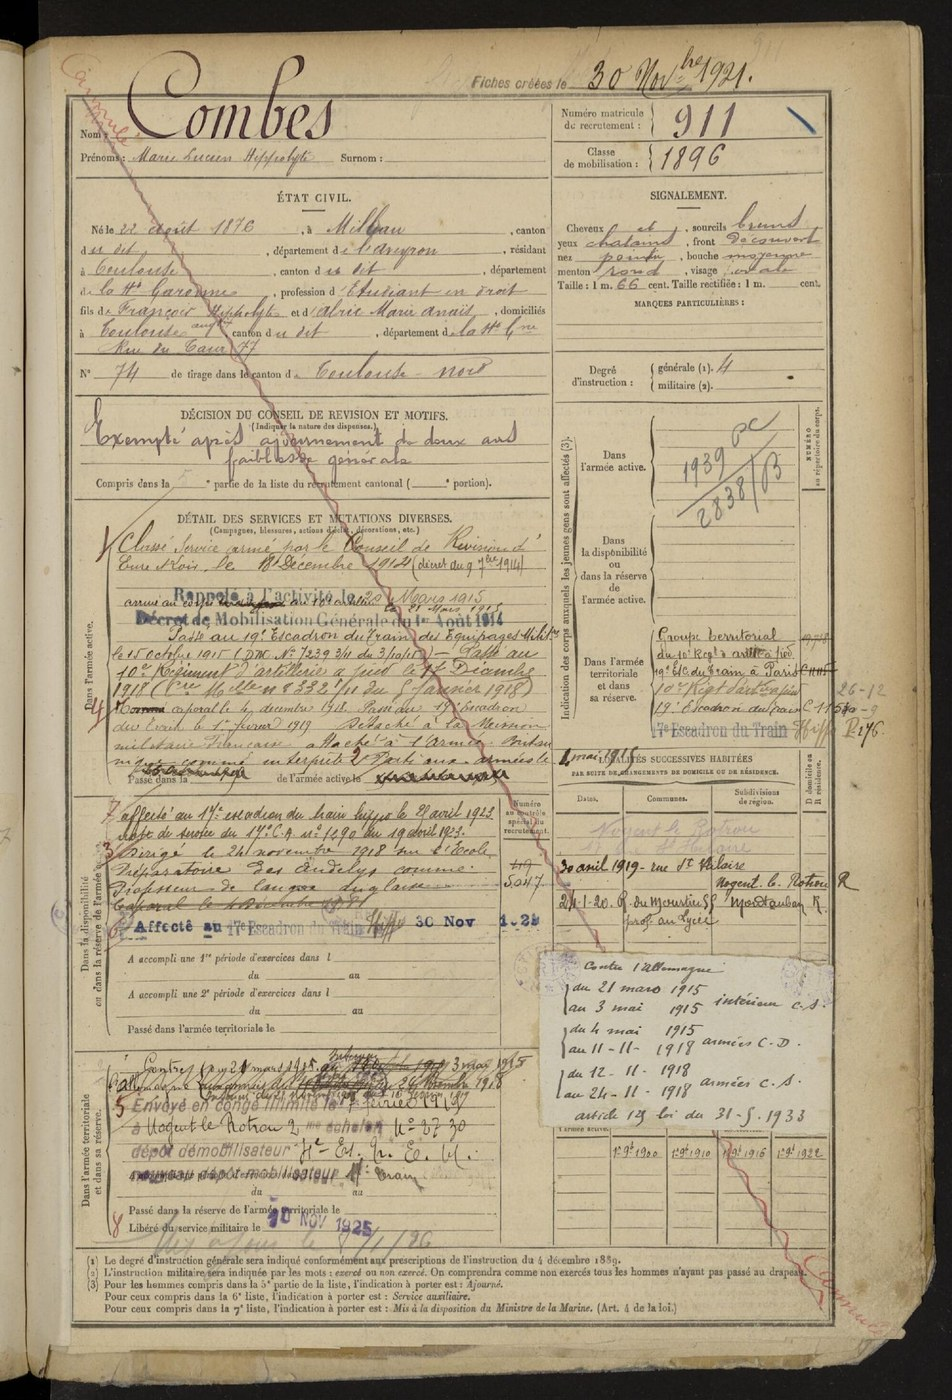
\includegraphics[width=0.94\linewidth,height=22mm,keepaspectratio]{illustrations/fiche_matricule.jpg}}
    \par\vspace{0.6mm}{\fontsize{5.8pt}{6.7pt}\selectfont Extrait du registre matricule d'Hippolyte Combes (classe 1896, matricule 911, bureau de recrutement de Toulouse) détaillant ses services auprès de la Mission militaire française attachée à l'Armée britannique (4 mai 1915 -- 11 novembre 1918).}
  \end{minipage}
\end{center}
\clearpage

% =============================================================================
% VIS-A-VIS SPREAD : SCAN #067 (20251126_103816.jpg) — Vue 067
% =============================================================================
\cleardoubleevenpage
% --- En-tête du folio (Page paire / gauche : Transcription, apparat & double registre) ---
\noindent\rule{\textwidth}{0.5pt}\par\vspace{0.6mm}
\noindent\textbf{\footnotesize SCAN \#067 — VUE 067} \hfill {\scriptsize\texttt{20251126\_\allowbreak 103816.jpg}}\par\vspace{0.3mm}
\noindent{\fontsize{7.0pt}{8.2pt}\selectfont Installation au hameau de Barlette (Ribeaucourt) et visa de permission à Bernaville}\par\vspace{0.25mm}
\noindent{\fontsize{7.0pt}{8.2pt}\selectfont\textit{Vendredi 6 octobre 1916 (après-midi et soir)} \hfill \textit{Hameau de Barlette (Ribeaucourt) et Bernaville (Somme)}}\par\vspace{0.6mm}
\noindent\rule{\textwidth}{0.35pt}\par\vspace{1.0mm}
% --- Corps de la transcription diplomatique et apparat marginal en prolongement ---
{\renewcommand{\arraystretch}{1.02}%
\noindent\hspace*{3.5mm}\begin{tabular}{@{}p{100mm}@{\hspace{3.5mm}}p{55mm}@{}}
      \leavevmode\fontsize{7.8pt}{9.2pt}\selectfont\strut Ven. 6 \hfill{} Oct / 16\strut & \leavevmode\fontsize{6.3pt}{7.2pt}\selectfont\raggedright\arraybackslash\color{black!88}\textbf{1} \textbf{Ven.} \textit{vendredi} ; \textbf{Oct} \textit{octobre}. \\
      \leavevmode\fontsize{7.8pt}{9.2pt}\selectfont\strut Ma Coy, cantonnée au hameau\strut & \leavevmode\fontsize{6.3pt}{7.2pt}\selectfont\raggedright\arraybackslash\color{black!88}\textbf{2} \textbf{Coy} \textit{Company : compagnie}. \\
      \leavevmode\fontsize{7.8pt}{9.2pt}\selectfont\strut de Barlette, près de Ribeaucourt\strut &  \\
      \leavevmode\fontsize{7.8pt}{9.2pt}\selectfont\strut qq maisons. Population très symphe\strut & \leavevmode\fontsize{6.3pt}{7.2pt}\selectfont\raggedright\arraybackslash\color{black!88}\textbf{4} \textbf{qq} \textit{quelques} ; \textbf{symphe} \textit{sympathique}. \\
      \leavevmode\llap{\fontsize{6.5pt}{7.5pt}\selectfont\color{darkgray}5\hspace{1.8mm}}\fontsize{7.8pt}{9.2pt}\selectfont\strut Région très boisée, extt pittoresque\strut & \leavevmode\fontsize{6.3pt}{7.2pt}\selectfont\raggedright\arraybackslash\color{black!88}\textbf{5} \textbf{extt} \textit{extrêmement}. \\
      \leavevmode\fontsize{7.8pt}{9.2pt}\selectfont\strut Après lunch, venu sur 1 lorry\strut & \leavevmode\fontsize{6.3pt}{7.2pt}\selectfont\raggedright\arraybackslash\color{black!88}\textbf{6} \textbf{lunch} \textit{angl.} déjeuner ; \textbf{lorry} \textit{angl.} camion. \\
      \leavevmode\fontsize{7.8pt}{9.2pt}\selectfont\strut à Bernaville et visé mon titre de\strut &  \\
      \leavevmode\fontsize{7.8pt}{9.2pt}\selectfont\strut permission au bureau de la Mission Fse\strut & \leavevmode\fontsize{6.3pt}{7.2pt}\selectfont\raggedright\arraybackslash\color{black!88}\textbf{8} \textbf{Fse} \textit{française}. \\
      \leavevmode\fontsize{7.8pt}{9.2pt}\selectfont\strut Bientôt trouvé 1 billet = gde\strut & \leavevmode\fontsize{6.3pt}{7.2pt}\selectfont\raggedright\arraybackslash\color{black!88}\textbf{9} \textbf{billet} \textit{angl.} logement de cantonnement ; \textbf{=} équivalence explicative : c’est-à-dire une grande chambre ; \textbf{gde} \textit{grande}. \\
      \leavevmode\llap{\fontsize{6.5pt}{7.5pt}\selectfont\color{darkgray}10\hspace{1.8mm}}\fontsize{7.8pt}{9.2pt}\selectfont\strut chambre, chz Mme Ve —\strut & \leavevmode\fontsize{6.3pt}{7.2pt}\selectfont\raggedright\arraybackslash\color{black!88}\textbf{10} \textbf{chz} \textit{chez} ; \textbf{Mme} \textit{Madame} ; \textbf{Ve} Veuve est le développement probable ; le cliché ne fournit pas un patronyme développé à sa suite. \\
      \leavevmode\fontsize{7.8pt}{9.2pt}\selectfont\strut à 900 mètres de Barlette\strut &  \\
      \leavevmode\fontsize{7.8pt}{9.2pt}\selectfont\strut Ameublement très sommaire, mais\strut &  \\
      \leavevmode\fontsize{7.8pt}{9.2pt}\selectfont\strut chambre très belle \& spacieuse\strut &  \\
      \leavevmode\fontsize{7.8pt}{9.2pt}\selectfont\strut A Doullens, Cartes ples : 50 c\strut & \leavevmode\fontsize{6.3pt}{7.2pt}\selectfont\raggedright\arraybackslash\color{black!88}\textbf{14} \textbf{ples} \textit{postales}. \\
      \leavevmode\llap{\fontsize{6.5pt}{7.5pt}\selectfont\color{darkgray}15\hspace{1.8mm}}\fontsize{7.8pt}{9.2pt}\selectfont\strut A ", canteen : 20, 20, 20, 20 c\strut & \leavevmode\fontsize{6.3pt}{7.2pt}\selectfont\raggedright\arraybackslash\color{black!88}\textbf{15} \textbf{"} signe de répétition renvoyant à Doullens, à la ligne précédente ; \textbf{canteen} \textit{angl.} cantine. \\
      \leavevmode\fontsize{7.8pt}{9.2pt}\selectfont\strut A Bernaville, cartes ples : 10 c\strut & \leavevmode\fontsize{6.3pt}{7.2pt}\selectfont\raggedright\arraybackslash\color{black!88}\textbf{16} \textbf{ples} \textit{postales}. \\
      \leavevmode\fontsize{7.8pt}{9.2pt}\selectfont\strut A Barlette : Tip au driver du lorry : 1f\strut & \leavevmode\fontsize{6.3pt}{7.2pt}\selectfont\raggedright\arraybackslash\color{black!88}\textbf{17} \textbf{Tip} \textit{angl.} pourboire ; \textbf{driver} \textit{angl.} conducteur ; \textbf{lorry} \textit{angl.} camion. \\
      \leavevmode\fontsize{7.8pt}{9.2pt}\selectfont\strut Gift au Q.M.S. Tait : 5 fr. –\strut & \leavevmode\fontsize{6.3pt}{7.2pt}\selectfont\raggedright\arraybackslash\color{black!88}\textbf{18} \textbf{Gift} \textit{angl.} cadeau ; somme donnée ; \textbf{Q.M.S.} \textit{Quartermaster Sergeant : sous-officier chargé de l’approvisionnement}. \\
\end{tabular}}%
\par\vspace*{\fill}
% --- Deux registres de commentaires en bas de page (sans intitulés, distingués par filets et mise en page) ---
\noindent\rule{\textwidth}{0.5pt}\par\vspace{0.8mm}
{\fontsize{6.8pt}{8.0pt}\selectfont%
\noindent\normalfont Le signe = introduit l’explication du billet, logement de cantonnement ; le signe de répétition du compte reprend Doullens. Ve après Mme est vraisemblablement l’abréviation de veuve, sans patronyme développé assuré. Un trait horizontal sépare les dépenses du récit. Les intitulés anglais Tip, driver et Gift reçoivent une traduction, comme lunch, lorry et canteen.\par\vspace{0.75mm}
\noindent\rule{38mm}{0.4pt}\par\vspace{0.65mm}
\noindent\hspace*{5mm}\parbox{\dimexpr\textwidth-5mm\relax}{\fontsize{6.8pt}{8.0pt}\selectfont\color{black!82}\textbf{Cantonnement :} La compagnie retrouvée en 066 cantonne à Barlette, près de Ribeaucourt. Combes fait viser son titre de permission à Bernaville, puis trouve une grande chambre à 900 mètres de Barlette. Le compte porte un cadeau 5 fr au Q.M.S. Tait, nom encore proposé. Les lignes n’attribuent pas à Tait une identité complète, ni à la maison la localisation exacte du camp. Le rapprochement avec le 18th Divisional Train est celui documenté en 066.}\par}
\newpage
% --- En-tête du fac-similé (Page impaire / droite : Scan original) ---
\noindent\rule{\textwidth}{0.5pt}\par\vspace{0.6mm}
\noindent\textbf{\fontsize{6.5pt}{7.6pt}\selectfont FAC-SIMILÉ EN VIS-À-VIS — VUE 067 (SCAN \#067)} \hfill {\fontsize{6.5pt}{7.6pt}\selectfont\texttt{20251126\_\allowbreak 103816.jpg}}\par\vspace{0.3mm}
\noindent{\fontsize{6.8pt}{8pt}\selectfont\textit{Livre-Journal d'Hippolyte Combes} — Vendredi 6 octobre 1916 (après-midi et soir) (Hameau de Barlette (Ribeaucourt) et Bernaville (Somme))}\par\vspace{0.6mm}
\noindent\rule{\textwidth}{0.35pt}\par\vspace*{\fill}
{\centering
  \setlength{\fboxsep}{1.2mm}%
  \setlength{\fboxrule}{0.4pt}%
  \fcolorbox{gray!55}{white}{%
    \includegraphics[width=0.94\textwidth,height=0.76\textheight,keepaspectratio]{\facsimiledir/20251126_103816.jpg}%
  }\par}
\vspace*{\fill}
\noindent\rule{\textwidth}{0.35pt}\par\vspace{0.5mm}
\noindent{\fontsize{6pt}{7.1pt}\selectfont\raggedright\color{darkgray}\textbf{Source :} Archives familiales Combes — Cliché numérique \texttt{20251126\_\allowbreak 103816.jpg} (Scan \#067/186, Vue 067). Haute définition : \texttt{scans\_haute\_qualite/\allowbreak 20251126\_\allowbreak 103816.jpg} ; version allégée : \texttt{scans\_compresses/\allowbreak 20251126\_\allowbreak 103816.jpg}.\par}
\newpage

% =============================================================================
% VIS-A-VIS SPREAD : SCAN #068 (20251126_103828.jpg) — Vue 068
% =============================================================================
\cleardoubleevenpage
% --- En-tête du folio (Page paire / gauche : Transcription, apparat & double registre) ---
\noindent\rule{\textwidth}{0.5pt}\par\vspace{0.6mm}
\noindent\textbf{\footnotesize SCAN \#068 — VUE 068} \hfill {\scriptsize\texttt{20251126\_\allowbreak 103828.jpg}}\par\vspace{0.3mm}
\noindent{\fontsize{7.0pt}{8.2pt}\selectfont Tempête nocturne sur les vergers de Barlette et règlement des frais de mess au capitaine Panton}\par\vspace{0.25mm}
\noindent{\fontsize{7.0pt}{8.2pt}\selectfont\textit{Samedi 7 octobre 1916} \hfill \textit{Hameau de Barlette, Ribeaucourt (Somme)}}\par\vspace{0.6mm}
\noindent\rule{\textwidth}{0.35pt}\par\vspace{1.0mm}
% --- Corps de la transcription diplomatique et apparat marginal en prolongement ---
{\renewcommand{\arraystretch}{1.02}%
\noindent\hspace*{3.5mm}\begin{tabular}{@{}p{100mm}@{\hspace{3.5mm}}p{55mm}@{}}
      \leavevmode\fontsize{7.8pt}{9.2pt}\selectfont\strut Sam. 7. \hfill{} Octbre 1916\strut & \leavevmode\fontsize{6.3pt}{7.2pt}\selectfont\raggedright\arraybackslash\color{black!88}\textbf{1} \textbf{Sam.} \textit{samedi} ; \textbf{Octbre} \textit{octobre}. \\
      \leavevmode\fontsize{7.8pt}{9.2pt}\selectfont\strut Bonne nuit de repos s/ lit improvisé.\strut & \leavevmode\fontsize{6.3pt}{7.2pt}\selectfont\raggedright\arraybackslash\color{black!88}\textbf{2} \textbf{s/} \textit{sur}. \\
      \leavevmode\fontsize{7.8pt}{9.2pt}\selectfont\strut Levé vers 6H 1/2 et commencé à m'installer. Ouvert sacs\strut &  \\
      \leavevmode\fontsize{7.8pt}{9.2pt}\selectfont\strut Durant nuit, averses torrentielles et rafales.\strut &  \\
      \leavevmode\llap{\fontsize{6.5pt}{7.5pt}\selectfont\color{darkgray}5\hspace{1.8mm}}\fontsize{7.8pt}{9.2pt}\selectfont\strut Les arbres et les arbustes, en face maison,\strut &  \\
      \leavevmode\fontsize{7.8pt}{9.2pt}\selectfont\strut tourmentés par le vent, bruissaient plaintivt\strut & \leavevmode\fontsize{6.3pt}{7.2pt}\selectfont\raggedright\arraybackslash\color{black!88}\textbf{6} \textbf{plaintivt} \textit{plaintivement}. \\
      \leavevmode\fontsize{7.8pt}{9.2pt}\selectfont\strut – On se serait cru près de la mer.\strut &  \\
      \leavevmode\fontsize{7.8pt}{9.2pt}\selectfont\strut Tout le jour, pluie et bourrasques.\strut &  \\
      \leavevmode\fontsize{7.8pt}{9.2pt}\selectfont\strut ciel couvert de gros nuages – –\strut &  \\
      \leavevmode\llap{\fontsize{6.5pt}{7.5pt}\selectfont\color{darkgray}10\hspace{1.8mm}}\fontsize{7.8pt}{9.2pt}\selectfont\strut Me plais bp ds mon billet. Ai très\strut & \leavevmode\fontsize{6.3pt}{7.2pt}\selectfont\raggedright\arraybackslash\color{black!88}\textbf{10} \textbf{bp} \textit{beaucoup} ; \textbf{ds} \textit{dans} ; \textbf{billet} \textit{angl.} logement de cantonnement. \\
      \leavevmode\fontsize{7.8pt}{9.2pt}\selectfont\strut gde chambre, haute de plafond. C'était le\strut & \leavevmode\fontsize{6.3pt}{7.2pt}\selectfont\raggedright\arraybackslash\color{black!88}\textbf{11} \textbf{gde} \textit{grande}. \\
      \leavevmode\fontsize{7.8pt}{9.2pt}\selectfont\strut salon — vieille gd-mère, extt sympathique\strut & \leavevmode\fontsize{6.3pt}{7.2pt}\selectfont\raggedright\arraybackslash\color{black!88}\textbf{12} \textbf{gd-mère} \textit{grand-mère} ; \textbf{extt} \textit{extrêmement}. \\
      \leavevmode\fontsize{7.8pt}{9.2pt}\selectfont\strut Devant maison, pâture ac pommiers\strut & \leavevmode\fontsize{6.3pt}{7.2pt}\selectfont\raggedright\arraybackslash\color{black!88}\textbf{13} \textbf{ac} \textit{avec}. \\
      \leavevmode\fontsize{7.8pt}{9.2pt}\selectfont\strut chargés de fruit Au delà, gds bois. –\strut & \leavevmode\fontsize{6.3pt}{7.2pt}\selectfont\raggedright\arraybackslash\color{black!88}\textbf{14} \textbf{gds} \textit{grands}. \\
      \leavevmode\llap{\fontsize{6.5pt}{7.5pt}\selectfont\color{darkgray}15\hspace{1.8mm}}\fontsize{7.8pt}{9.2pt}\selectfont\strut Au Cap. Panton payé ma part dépenses\strut & \leavevmode\fontsize{6.3pt}{7.2pt}\selectfont\raggedright\arraybackslash\color{black!88}\textbf{15} \textbf{Cap.} \textit{capitaine}. \\
      \leavevmode\fontsize{7.8pt}{9.2pt}\selectfont\strut mess en septbre, pour — — jours : 29 f —\strut & \leavevmode\fontsize{6.3pt}{7.2pt}\selectfont\raggedright\arraybackslash\color{black!88}\textbf{16} \textbf{mess} \textit{angl.} table commune des officiers ; popote ; \textbf{septbre} \textit{septembre} ; \textbf{— —} tirets autographes : le nombre des journées n’est pas renseigné. \\
\end{tabular}}%
\par\vspace*{\fill}
% --- Deux registres de commentaires en bas de page (sans intitulés, distingués par filets et mise en page) ---
\noindent\rule{\textwidth}{0.5pt}\par\vspace{0.8mm}
{\fontsize{6.8pt}{8.0pt}\selectfont%
\noindent\normalfont Le nombre de journées de mess est laissé non renseigné entre pour et jours, par des tirets autographes ; il ne s’agit pas d’une perte matérielle du support. La contraction ac signifie avec et gd-mère se développe grand-mère. Le billet est le logement de cantonnement. Le compte inférieur, consacré à la popote de septembre, est séparé du récit par un trait horizontal.\par\vspace{0.75mm}
\noindent\rule{38mm}{0.4pt}\par\vspace{0.65mm}
\noindent\hspace*{5mm}\parbox{\dimexpr\textwidth-5mm\relax}{\fontsize{6.8pt}{8.0pt}\selectfont\color{black!82}\textbf{Chambre etmess :} Le 7 octobre, Combes s’installe dans un ancien salon, devant une pâture aux pommiers et de grands bois ; il décrit le vent et la pluie. Il paie au Cap. Panton 29 f pour sa part des dépenses du mess en septembre. Le nombre de jours est laissé vide dans le compte. Une moyenne de 2 f 20 par jour ou le rôle de gérant attribué au capitaine ne se déduisent pas de cette somme.}\par}
\newpage
% --- En-tête du fac-similé (Page impaire / droite : Scan original) ---
\noindent\rule{\textwidth}{0.5pt}\par\vspace{0.6mm}
\noindent\textbf{\fontsize{6.5pt}{7.6pt}\selectfont FAC-SIMILÉ EN VIS-À-VIS — VUE 068 (SCAN \#068)} \hfill {\fontsize{6.5pt}{7.6pt}\selectfont\texttt{20251126\_\allowbreak 103828.jpg}}\par\vspace{0.3mm}
\noindent{\fontsize{6.8pt}{8pt}\selectfont\textit{Livre-Journal d'Hippolyte Combes} — Samedi 7 octobre 1916 (Hameau de Barlette, Ribeaucourt (Somme))}\par\vspace{0.6mm}
\noindent\rule{\textwidth}{0.35pt}\par\vspace*{\fill}
{\centering
  \setlength{\fboxsep}{1.2mm}%
  \setlength{\fboxrule}{0.4pt}%
  \fcolorbox{gray!55}{white}{%
    \includegraphics[width=0.94\textwidth,height=0.76\textheight,keepaspectratio]{\facsimiledir/20251126_103828.jpg}%
  }\par}
\vspace*{\fill}
\noindent\rule{\textwidth}{0.35pt}\par\vspace{0.5mm}
\noindent{\fontsize{6pt}{7.1pt}\selectfont\raggedright\color{darkgray}\textbf{Source :} Archives familiales Combes — Cliché numérique \texttt{20251126\_\allowbreak 103828.jpg} (Scan \#068/186, Vue 068). Haute définition : \texttt{scans\_haute\_qualite/\allowbreak 20251126\_\allowbreak 103828.jpg} ; version allégée : \texttt{scans\_compresses/\allowbreak 20251126\_\allowbreak 103828.jpg}.\par}
\newpage

% =============================================================================
% VIS-A-VIS SPREAD : SCAN #069 (20251126_103845.jpg) — Vue 069
% =============================================================================
\cleardoubleevenpage
% --- En-tête du folio (Page paire / gauche : Transcription, apparat & double registre) ---
\noindent\rule{\textwidth}{0.5pt}\par\vspace{0.6mm}
\noindent\textbf{\footnotesize SCAN \#069 — VUE 069} \hfill {\scriptsize\texttt{20251126\_\allowbreak 103845.jpg}}\par\vspace{0.3mm}
\noindent{\fontsize{7.0pt}{8.2pt}\selectfont Dimanche de repos à Barlette et perception de la solde à pied à Bernaville sous la rafale}\par\vspace{0.25mm}
\noindent{\fontsize{7.0pt}{8.2pt}\selectfont\textit{Dimanche 8 octobre 1916} \hfill \textit{Barlette (Ribeaucourt) et Bernaville (Somme)}}\par\vspace{0.6mm}
\noindent\rule{\textwidth}{0.35pt}\par\vspace{1.0mm}
% --- Corps de la transcription diplomatique et apparat marginal en prolongement ---
{\renewcommand{\arraystretch}{1.02}%
\noindent\hspace*{3.5mm}\begin{tabular}{@{}p{100mm}@{\hspace{3.5mm}}p{55mm}@{}}
      \leavevmode\fontsize{7.8pt}{9.2pt}\selectfont\strut Dim. 8. \hfill{} Octb 1916\strut & \leavevmode\fontsize{6.3pt}{7.2pt}\selectfont\raggedright\arraybackslash\color{black!88}\textbf{1} \textbf{Dim.} \textit{dimanche} ; \textbf{Octb} \textit{octobre}. \\
      \leavevmode\fontsize{7.8pt}{9.2pt}\selectfont\strut Installation terminée...\strut &  \\
      \leavevmode\fontsize{7.8pt}{9.2pt}\selectfont\strut Jouis repos complet village paisible\strut & \leavevmode\fontsize{6.3pt}{7.2pt}\selectfont\raggedright\arraybackslash\color{black!88}\textbf{3} \textbf{Jouis repos complet village paisible} Construction verbale elliptique : les prépositions et articles attendus ne sont pas écrits. \\
      \leavevmode\fontsize{7.8pt}{9.2pt}\selectfont\strut Tout le jour, ciel couvert de nuages\strut &  \\
      \leavevmode\llap{\fontsize{6.5pt}{7.5pt}\selectfont\color{darkgray}5\hspace{1.8mm}}\fontsize{7.8pt}{9.2pt}\selectfont\strut que le vent chassait avec violence\strut &  \\
      \leavevmode\fontsize{7.8pt}{9.2pt}\selectfont\strut Après-midi, venu à Bernaville,\strut &  \\
      \leavevmode\fontsize{7.8pt}{9.2pt}\selectfont\strut au bureau de la mission fse –\strut & \leavevmode\fontsize{6.3pt}{7.2pt}\selectfont\raggedright\arraybackslash\color{black!88}\textbf{7} \textbf{fse} \textit{française}. \\
      \leavevmode\fontsize{7.8pt}{9.2pt}\selectfont\strut Aller \& retour à pied. Violentes rafales\strut &  \\
      \leavevmode\fontsize{7.8pt}{9.2pt}\selectfont\strut Pays très verdoyant \& boisé.\strut &  \\
      \leavevmode\llap{\fontsize{6.5pt}{7.5pt}\selectfont\color{darkgray}10\hspace{1.8mm}}\fontsize{7.8pt}{9.2pt}\selectfont\strut A Bernaville, solde \& indemnité : 78 f 75\strut & \leavevmode\fontsize{6.3pt}{7.2pt}\selectfont\raggedright\arraybackslash\color{black!88}\textbf{10} \textbf{A Bernaville} La recette de solde et indemnité est isolée au bas de la page sous un trait horizontal. \\
\end{tabular}}%
\par\vspace*{\fill}
% --- Deux registres de commentaires en bas de page (sans intitulés, distingués par filets et mise en page) ---
\noindent\rule{\textwidth}{0.5pt}\par\vspace{0.8mm}
{\fontsize{6.8pt}{8.0pt}\selectfont%
\noindent\normalfont Jouis est un verbe et non le premier terme d’une juxtaposition nominale : la phrase condense le complément et les indications de lieu sans écrire toutes les prépositions ou tous les articles. Rien ne permet d’y supposer une lacune matérielle. La seule mention comptable est isolée au bas de la page par un trait horizontal.\par\vspace{0.75mm}
\noindent\rule{38mm}{0.4pt}\par\vspace{0.65mm}
\noindent\hspace*{5mm}\parbox{\dimexpr\textwidth-5mm\relax}{\fontsize{6.8pt}{8.0pt}\selectfont\color{black!82}\textbf{Bernaville :} Le 8 octobre, après l’installation, Combes fait l’aller-retour à pied au bureau de la mission française à Bernaville. Il note 78 f 75 de solde et indemnité. La périodicité de quinzaine n’est pas indiquée. Le contexte de sa compagnie est attesté par 066–067 ; il ne suffit pas à préciser à lui seul l’organisation de ce bureau de mission.}\par}
\newpage
% --- En-tête du fac-similé (Page impaire / droite : Scan original) ---
\noindent\rule{\textwidth}{0.5pt}\par\vspace{0.6mm}
\noindent\textbf{\fontsize{6.5pt}{7.6pt}\selectfont FAC-SIMILÉ EN VIS-À-VIS — VUE 069 (SCAN \#069)} \hfill {\fontsize{6.5pt}{7.6pt}\selectfont\texttt{20251126\_\allowbreak 103845.jpg}}\par\vspace{0.3mm}
\noindent{\fontsize{6.8pt}{8pt}\selectfont\textit{Livre-Journal d'Hippolyte Combes} — Dimanche 8 octobre 1916 (Barlette (Ribeaucourt) et Bernaville (Somme))}\par\vspace{0.6mm}
\noindent\rule{\textwidth}{0.35pt}\par\vspace*{\fill}
{\centering
  \setlength{\fboxsep}{1.2mm}%
  \setlength{\fboxrule}{0.4pt}%
  \fcolorbox{gray!55}{white}{%
    \includegraphics[width=0.94\textwidth,height=0.76\textheight,keepaspectratio]{\facsimiledir/20251126_103845.jpg}%
  }\par}
\vspace*{\fill}
\noindent\rule{\textwidth}{0.35pt}\par\vspace{0.5mm}
\noindent{\fontsize{6pt}{7.1pt}\selectfont\raggedright\color{darkgray}\textbf{Source :} Archives familiales Combes — Cliché numérique \texttt{20251126\_\allowbreak 103845.jpg} (Scan \#069/186, Vue 069). Haute définition : \texttt{scans\_haute\_qualite/\allowbreak 20251126\_\allowbreak 103845.jpg} ; version allégée : \texttt{scans\_compresses/\allowbreak 20251126\_\allowbreak 103845.jpg}.\par}
\newpage

% =============================================================================
% VIS-A-VIS SPREAD : SCAN #070 (20251126_103857.jpg) — Vue 070
% =============================================================================
\cleardoubleevenpage
% --- En-tête du folio (Page paire / gauche : Transcription, apparat & double registre) ---
\noindent\rule{\textwidth}{0.5pt}\par\vspace{0.6mm}
\noindent\textbf{\footnotesize SCAN \#070 — VUE 070} \hfill {\scriptsize\texttt{20251126\_\allowbreak 103857.jpg}}\par\vspace{0.3mm}
\noindent{\fontsize{7.0pt}{8.2pt}\selectfont Promenade forestière et clair de lune d’octobre}\par\vspace{0.25mm}
\noindent{\fontsize{7.0pt}{8.2pt}\selectfont\textit{Lundi 9 octobre 1916} \hfill \textit{Barlette et forêt de Ribeaucourt (Somme)}}\par\vspace{0.6mm}
\noindent\rule{\textwidth}{0.35pt}\par\vspace{1.0mm}
% --- Corps de la transcription diplomatique et apparat marginal en prolongement ---
{\renewcommand{\arraystretch}{0.95}%
\noindent\hspace*{3.5mm}\begin{tabular}{@{}p{100mm}@{\hspace{3.5mm}}p{55mm}@{}}
      \leavevmode\fontsize{7.4pt}{8.6pt}\selectfont\strut Lundi 9 \hfill{} Oct – / 16\strut & \leavevmode\fontsize{6.3pt}{7.2pt}\selectfont\raggedright\arraybackslash\color{black!88}\textbf{1} \textbf{Oct} \textit{octobre}. \\
      \leavevmode\fontsize{7.4pt}{8.6pt}\selectfont\strut Tout le jour, ciel assombri gros nuages\strut &  \\
      \leavevmode\fontsize{7.4pt}{8.6pt}\selectfont\strut couleur de plomb\strut &  \\
      \leavevmode\fontsize{7.4pt}{8.6pt}\selectfont\strut Après-midi, pénétré forêt qui s'étend à 1\strut &  \\
      \leavevmode\llap{\fontsize{6.5pt}{7.5pt}\selectfont\color{darkgray}5\hspace{1.8mm}}\fontsize{7.4pt}{8.6pt}\selectfont\strut faible distance de la route et parallelt –\strut & \leavevmode\fontsize{6.3pt}{7.2pt}\selectfont\raggedright\arraybackslash\color{black!88}\textbf{5} \textbf{parallelt} \textit{parallèlement}. \\
      \leavevmode\fontsize{7.4pt}{8.6pt}\selectfont\strut Sentiers encore boueux et jonchés de feuilles rouillées.\strut &  \\
      \leavevmode\fontsize{7.4pt}{8.6pt}\selectfont\strut Feuillages épais \& verts. Ds les taillis, enchevêtrt\strut & \leavevmode\fontsize{6.3pt}{7.2pt}\selectfont\raggedright\arraybackslash\color{black!88}\textbf{7} \textbf{Ds} \textit{Dans} ; \textbf{enchevêtrt} \textit{enchevêtrement}. \\
      \leavevmode\fontsize{7.4pt}{8.6pt}\selectfont\strut d'arbustes \& de lianes. Des troncs énormes\strut &  \\
      \leavevmode\fontsize{7.4pt}{8.6pt}\selectfont\strut s'élèvent très haut, arbres plusis fois\strut & \leavevmode\fontsize{6.3pt}{7.2pt}\selectfont\raggedright\arraybackslash\color{black!88}\textbf{9} \textbf{plusis} \textit{plusieurs}. \\
      \leavevmode\llap{\fontsize{6.5pt}{7.5pt}\selectfont\color{darkgray}10\hspace{1.8mm}}\fontsize{7.4pt}{8.6pt}\selectfont\strut séculaires. Resté lgt ds cet océan de\strut & \leavevmode\fontsize{6.3pt}{7.2pt}\selectfont\raggedright\arraybackslash\color{black!88}\textbf{10} \textbf{lgt} \textit{longtemps} ; \textbf{ds} \textit{dans}. \\
      \leavevmode\fontsize{7.4pt}{8.6pt}\selectfont\strut verdure. Ecouté, ravi, le bruissement\strut &  \\
      \leavevmode\fontsize{7.4pt}{8.6pt}\selectfont\strut du vent à travers les branches\strut &  \\
      \leavevmode\fontsize{7.4pt}{8.6pt}\selectfont\strut feuillues\strut &  \\
      \leavevmode\fontsize{7.4pt}{8.6pt}\selectfont\strut Le soir, en revenant du mess,\strut & \leavevmode\fontsize{6.3pt}{7.2pt}\selectfont\raggedright\arraybackslash\color{black!88}\textbf{14} \textbf{mess} \textit{angl.} table commune des officiers ; popote. \\
      \leavevmode\llap{\fontsize{6.5pt}{7.5pt}\selectfont\color{darkgray}15\hspace{1.8mm}}\fontsize{7.4pt}{8.6pt}\selectfont\strut admiré ciel [mervt ?] éclairé par lune [ajout interl. : pleine].\strut & \leavevmode\fontsize{6.3pt}{7.2pt}\selectfont\raggedright\arraybackslash\color{black!88}\textbf{15} \textbf{[mervt ?]} Contraction proposée pour merveilleusement ; lecture réservée ; \textbf{pleine} Mot ajouté sous lune, dans l’interligne. \\
      \leavevmode\fontsize{7.4pt}{8.6pt}\selectfont\strut qq étoiles, çà et là. Campagne curieuse\strut & \leavevmode\fontsize{6.3pt}{7.2pt}\selectfont\raggedright\arraybackslash\color{black!88}\textbf{16} \textbf{qq} \textit{quelques}. \\
      \leavevmode\fontsize{7.4pt}{8.6pt}\selectfont\strut à regarder les moindres details, bien\strut &  \\
      \leavevmode\fontsize{7.4pt}{8.6pt}\selectfont\strut détachés –\strut &  \\
      \leavevmode\fontsize{7.4pt}{8.6pt}\selectfont\strut Me plais infinimt ds ma gde et\strut & \leavevmode\fontsize{6.3pt}{7.2pt}\selectfont\raggedright\arraybackslash\color{black!88}\textbf{19} \textbf{infinimt} \textit{infiniment} ; \textbf{ds} \textit{dans} ; \textbf{gde} \textit{grande}. \\
      \leavevmode\llap{\fontsize{6.5pt}{7.5pt}\selectfont\color{darkgray}20\hspace{1.8mm}}\fontsize{7.4pt}{8.6pt}\selectfont\strut belle chambre, 1 vrai salon.\strut &  \\
\end{tabular}}%
\par\vspace*{\fill}
% --- Deux registres de commentaires en bas de page (sans intitulés, distingués par filets et mise en page) ---
\noindent\rule{\textwidth}{0.5pt}\par\vspace{0.8mm}
{\fontsize{6.8pt}{8.0pt}\selectfont%
\noindent\normalfont Pleine est une addition interlinéaire placée sous lune. La contraction après ciel reste proposée mervt, à développer éventuellement merveilleusement. Infinimt signifie infiniment ; ce développement, déjà cité dans l’ancien commentaire, manquait pourtant en marge. Campagne curieuse à regarder les moindres details conserve sa construction elliptique.\par\vspace{0.75mm}
\noindent\rule{38mm}{0.4pt}\par\vspace{0.65mm}
\noindent\hspace*{5mm}\parbox{\dimexpr\textwidth-5mm\relax}{\fontsize{6.8pt}{8.0pt}\selectfont\color{black!82}\textbf{Forêt et lune :} Le 9 octobre, Combes décrit une forêt proche de la route, des arbres qu’il juge plusieurs fois séculaires, puis le bruissement du vent. Le bois de Ribeaucourt, nommé le 11 octobre (vue 072), est un rapprochement géographique plausible ; cette vue ne nomme pas la forêt ni la route. Le retour du mess se fait sous la lune, et Combes note son plaisir dans la grande chambre. Il ne déclare pas une journée entière sans service.}\par}
\newpage
% --- En-tête du fac-similé (Page impaire / droite : Scan original) ---
\noindent\rule{\textwidth}{0.5pt}\par\vspace{0.6mm}
\noindent\textbf{\fontsize{6.5pt}{7.6pt}\selectfont FAC-SIMILÉ EN VIS-À-VIS — VUE 070 (SCAN \#070)} \hfill {\fontsize{6.5pt}{7.6pt}\selectfont\texttt{20251126\_\allowbreak 103857.jpg}}\par\vspace{0.3mm}
\noindent{\fontsize{6.8pt}{8pt}\selectfont\textit{Livre-Journal d'Hippolyte Combes} — Lundi 9 octobre 1916 (Barlette et forêt de Ribeaucourt (Somme))}\par\vspace{0.6mm}
\noindent\rule{\textwidth}{0.35pt}\par\vspace*{\fill}
{\centering
  \setlength{\fboxsep}{1.2mm}%
  \setlength{\fboxrule}{0.4pt}%
  \fcolorbox{gray!55}{white}{%
    \includegraphics[width=0.94\textwidth,height=0.76\textheight,keepaspectratio]{\facsimiledir/20251126_103857.jpg}%
  }\par}
\vspace*{\fill}
\noindent\rule{\textwidth}{0.35pt}\par\vspace{0.5mm}
\noindent{\fontsize{6pt}{7.1pt}\selectfont\raggedright\color{darkgray}\textbf{Source :} Archives familiales Combes — Cliché numérique \texttt{20251126\_\allowbreak 103857.jpg} (Scan \#070/186, Vue 070). Haute définition : \texttt{scans\_haute\_qualite/\allowbreak 20251126\_\allowbreak 103857.jpg} ; version allégée : \texttt{scans\_compresses/\allowbreak 20251126\_\allowbreak 103857.jpg}.\par}
\newpage

% =============================================================================
% VIS-A-VIS SPREAD : SCAN #071 (20251126_103913.jpg) — Vue 071
% =============================================================================
\cleardoubleevenpage
% --- En-tête du folio (Page paire / gauche : Transcription, apparat & double registre) ---
\noindent\rule{\textwidth}{0.5pt}\par\vspace{0.6mm}
\noindent\textbf{\footnotesize SCAN \#071 — VUE 071} \hfill {\scriptsize\texttt{20251126\_\allowbreak 103913.jpg}}\par\vspace{0.3mm}
\noindent{\fontsize{7.0pt}{8.2pt}\selectfont Corvée de fourrage vert en lisière des bois aux couleurs d'automne et nuit de pleine lune}\par\vspace{0.25mm}
\noindent{\fontsize{7.0pt}{8.2pt}\selectfont\textit{Mardi 10 octobre 1916} \hfill \textit{Barlette et bois de Ribeaucourt (Somme)}}\par\vspace{0.6mm}
\noindent\rule{\textwidth}{0.35pt}\par\vspace{1.0mm}
% --- Corps de la transcription diplomatique et apparat marginal en prolongement ---
{\renewcommand{\arraystretch}{1.02}%
\noindent\hspace*{3.5mm}\begin{tabular}{@{}p{100mm}@{\hspace{3.5mm}}p{55mm}@{}}
      \leavevmode\fontsize{7.8pt}{9.2pt}\selectfont\strut Mardi 10 \hfill{} Oct 1916\strut & \leavevmode\fontsize{6.3pt}{7.2pt}\selectfont\raggedright\arraybackslash\color{black!88}\textbf{1} \textbf{Oct} \textit{octobre}. \\
      \leavevmode\fontsize{7.8pt}{9.2pt}\selectfont\strut Enfin, très belle journée.\strut &  \\
      \leavevmode\fontsize{7.8pt}{9.2pt}\selectfont\strut Matin \& après-midi, occupé pour green\strut & \leavevmode\fontsize{6.3pt}{7.2pt}\selectfont\raggedright\arraybackslash\color{black!88}\textbf{3} \textbf{green} \textit{angl.} fourrage vert ; la locution anglaise green forage continue à la ligne suivante. \\
      \leavevmode\fontsize{7.8pt}{9.2pt}\selectfont\strut forage. Conduit fourragères ds les\strut & \leavevmode\fontsize{6.3pt}{7.2pt}\selectfont\raggedright\arraybackslash\color{black!88}\textbf{4} \textbf{ds} \textit{dans}. \\
      \leavevmode\llap{\fontsize{6.5pt}{7.5pt}\selectfont\color{darkgray}5\hspace{1.8mm}}\fontsize{7.8pt}{9.2pt}\selectfont\strut champs. Tout en surveillant le\strut &  \\
      \leavevmode\fontsize{7.8pt}{9.2pt}\selectfont\strut chargement, assis s/ 1 botte de\strut & \leavevmode\fontsize{6.3pt}{7.2pt}\selectfont\raggedright\arraybackslash\color{black!88}\textbf{6} \textbf{s/} \textit{sur}. \\
      \leavevmode\fontsize{7.8pt}{9.2pt}\selectfont\strut luzerne – et rempli yeux vue\strut & \leavevmode\fontsize{6.3pt}{7.2pt}\selectfont\raggedright\arraybackslash\color{black!88}\textbf{7} \textbf{rempli yeux vue} Construction elliptique : articles et préposition omis dans la notation du carnet. \\
      \leavevmode\fontsize{7.8pt}{9.2pt}\selectfont\strut des bois. Devant moi, à qq 40 ou 50\strut & \leavevmode\fontsize{6.3pt}{7.2pt}\selectfont\raggedright\arraybackslash\color{black!88}\textbf{8} \textbf{qq} \textit{quelque, au sens d’environ devant 40 ou 50 mètres}. \\
      \leavevmode\fontsize{7.8pt}{9.2pt}\selectfont\strut mètres, lisière forêt arbres\strut &  \\
      \leavevmode\llap{\fontsize{6.5pt}{7.5pt}\selectfont\color{darkgray}10\hspace{1.8mm}}\fontsize{7.8pt}{9.2pt}\selectfont\strut massés les 1 à côté des autres\strut &  \\
      \leavevmode\fontsize{7.8pt}{9.2pt}\selectfont\strut très belles teintes que le soleil rendait\strut &  \\
      \leavevmode\fontsize{7.8pt}{9.2pt}\selectfont\strut + éclatantes et qui se détachaient\strut &  \\
      \leavevmode\fontsize{7.8pt}{9.2pt}\selectfont\strut sur le ciel bleu –\strut &  \\
      \leavevmode\fontsize{7.8pt}{9.2pt}\selectfont\strut Comme ts les soirs, nuit\strut & \leavevmode\fontsize{6.3pt}{7.2pt}\selectfont\raggedright\arraybackslash\color{black!88}\textbf{14} \textbf{ts} \textit{tous}. \\
      \leavevmode\llap{\fontsize{6.5pt}{7.5pt}\selectfont\color{darkgray}15\hspace{1.8mm}}\fontsize{7.8pt}{9.2pt}\selectfont\strut merveilleuse. Lune pleine\strut &  \\
      \leavevmode\fontsize{7.8pt}{9.2pt}\selectfont\strut brillant d'1 vive lueur, ds l'immensité\strut & \leavevmode\fontsize{6.3pt}{7.2pt}\selectfont\raggedright\arraybackslash\color{black!88}\textbf{16} \textbf{ds} \textit{dans}. \\
      \leavevmode\fontsize{7.8pt}{9.2pt}\selectfont\strut firmament. qq rares étoiles\strut & \leavevmode\fontsize{6.3pt}{7.2pt}\selectfont\raggedright\arraybackslash\color{black!88}\textbf{17} \textbf{qq} \textit{quelques}. \\
      \leavevmode\fontsize{7.8pt}{9.2pt}\selectfont\strut gde paix épandue ——————\strut & \leavevmode\fontsize{6.3pt}{7.2pt}\selectfont\raggedright\arraybackslash\color{black!88}\textbf{18} \textbf{gde} \textit{grande}. \\
\end{tabular}}%
\par\vspace*{\fill}
% --- Deux registres de commentaires en bas de page (sans intitulés, distingués par filets et mise en page) ---
\noindent\rule{\textwidth}{0.5pt}\par\vspace{0.8mm}
{\fontsize{6.8pt}{8.0pt}\selectfont%
\noindent\normalfont Green forage est une seule expression anglaise, répartie sur deux lignes ; fourragères désigne les chariots à fourrage. Qq a deux valeurs dans cette page : quelque, environ, devant une estimation chiffrée ; quelques devant rares étoiles. Rempli yeux vue conserve ses ellipses et n’appelle pas de suppléments dans le texte.\par\vspace{0.75mm}
\noindent\rule{38mm}{0.4pt}\par\vspace{0.65mm}
\noindent\hspace*{5mm}\parbox{\dimexpr\textwidth-5mm\relax}{\fontsize{6.8pt}{8.0pt}\selectfont\color{black!82}\textbf{Fourrage vert :} Le 10 octobre, matin et après-midi sont occupés au green forage. Combes conduit des fourragères, surveille le chargement de luzerne et observe les bois à quelque 40 ou 50 mètres. Cette activité prolonge les corvées de fourrage des vues 049–050, après son retour à la 152 Coy en 066. La description des feuillages et de la lune accompagne ainsi une tâche de ravitaillement ; elle ne prouve pas l’usage de tout ce chargement par les seuls attelages de sa compagnie.}\par}
\newpage
% --- En-tête du fac-similé (Page impaire / droite : Scan original) ---
\noindent\rule{\textwidth}{0.5pt}\par\vspace{0.6mm}
\noindent\textbf{\fontsize{6.5pt}{7.6pt}\selectfont FAC-SIMILÉ EN VIS-À-VIS — VUE 071 (SCAN \#071)} \hfill {\fontsize{6.5pt}{7.6pt}\selectfont\texttt{20251126\_\allowbreak 103913.jpg}}\par\vspace{0.3mm}
\noindent{\fontsize{6.8pt}{8pt}\selectfont\textit{Livre-Journal d'Hippolyte Combes} — Mardi 10 octobre 1916 (Barlette et bois de Ribeaucourt (Somme))}\par\vspace{0.6mm}
\noindent\rule{\textwidth}{0.35pt}\par\vspace*{\fill}
{\centering
  \setlength{\fboxsep}{1.2mm}%
  \setlength{\fboxrule}{0.4pt}%
  \fcolorbox{gray!55}{white}{%
    \includegraphics[width=0.94\textwidth,height=0.76\textheight,keepaspectratio]{\facsimiledir/20251126_103913.jpg}%
  }\par}
\vspace*{\fill}
\noindent\rule{\textwidth}{0.35pt}\par\vspace{0.5mm}
\noindent{\fontsize{6pt}{7.1pt}\selectfont\raggedright\color{darkgray}\textbf{Source :} Archives familiales Combes — Cliché numérique \texttt{20251126\_\allowbreak 103913.jpg} (Scan \#071/186, Vue 071). Haute définition : \texttt{scans\_haute\_qualite/\allowbreak 20251126\_\allowbreak 103913.jpg} ; version allégée : \texttt{scans\_compresses/\allowbreak 20251126\_\allowbreak 103913.jpg}.\par}
\newpage

% =============================================================================
% VIS-A-VIS SPREAD : SCAN #072 (20251126_103948.jpg) — Vue 072
% =============================================================================
\cleardoubleevenpage
% --- En-tête du folio (Page paire / gauche : Transcription, apparat & double registre) ---
\noindent\rule{\textwidth}{0.5pt}\par\vspace{0.6mm}
\noindent\textbf{\footnotesize SCAN \#072 — VUE 072} \hfill {\scriptsize\texttt{20251126\_\allowbreak 103948.jpg}}\par\vspace{0.3mm}
\noindent{\fontsize{7.0pt}{8.2pt}\selectfont Convoi de luzerne sous une pluie battante derrière le grand bois de Ribeaucourt}\par\vspace{0.25mm}
\noindent{\fontsize{7.0pt}{8.2pt}\selectfont\textit{Mercredi 11 octobre 1916} \hfill \textit{Barlette et Ribeaucourt (Somme)}}\par\vspace{0.6mm}
\noindent\rule{\textwidth}{0.35pt}\par\vspace{1.0mm}
% --- Corps de la transcription diplomatique et apparat marginal en prolongement ---
{\renewcommand{\arraystretch}{1.02}%
\noindent\hspace*{3.5mm}\begin{tabular}{@{}p{100mm}@{\hspace{3.5mm}}p{55mm}@{}}
      \leavevmode\fontsize{7.8pt}{9.2pt}\selectfont\strut Mer. 11 \hfill{} Oct / 16\strut & \leavevmode\fontsize{6.3pt}{7.2pt}\selectfont\raggedright\arraybackslash\color{black!88}\textbf{1} \textbf{Mer.} \textit{mercredi} ; \textbf{Oct} \textit{octobre}. \\
      \leavevmode\fontsize{7.8pt}{9.2pt}\selectfont\strut Matinée employée de =\strut & \leavevmode\fontsize{6.3pt}{7.2pt}\selectfont\raggedright\arraybackslash\color{black!88}\textbf{2} \textbf{=} même : de même manière qu’hier. \\
      \leavevmode\fontsize{7.8pt}{9.2pt}\selectfont\strut manière qu'hier. Sous pluie battante,\strut &  \\
      \leavevmode\fontsize{7.8pt}{9.2pt}\selectfont\strut dû conduire wagons ds 1 champ de luzerne\strut & \leavevmode\fontsize{6.3pt}{7.2pt}\selectfont\raggedright\arraybackslash\color{black!88}\textbf{4} \textbf{ds} \textit{dans}. \\
      \leavevmode\llap{\fontsize{6.5pt}{7.5pt}\selectfont\color{darkgray}5\hspace{1.8mm}}\fontsize{7.8pt}{9.2pt}\selectfont\strut derrière le grand bois de Ribeaucourt\strut &  \\
      \leavevmode\fontsize{7.8pt}{9.2pt}\selectfont\strut Rentré billet, casque \& cape tt ruisselants\strut & \leavevmode\fontsize{6.3pt}{7.2pt}\selectfont\raggedright\arraybackslash\color{black!88}\textbf{6} \textbf{billet} \textit{angl.} logement de cantonnement ; \textbf{tt} \textit{tout, adverbe devant ruisselants}. \\
      \leavevmode\fontsize{7.8pt}{9.2pt}\selectfont\strut Après-midi, liberté entière –\strut &  \\
      \leavevmode\fontsize{7.8pt}{9.2pt}\selectfont\strut Tt le jour, ciel nuageux et temps\strut & \leavevmode\fontsize{6.3pt}{7.2pt}\selectfont\raggedright\arraybackslash\color{black!88}\textbf{8} \textbf{Tt} \textit{Tout}. \\
      \leavevmode\fontsize{7.8pt}{9.2pt}\selectfont\strut pluvieux. – –\strut &  \\
\end{tabular}}%
\par\vspace*{\fill}
% --- Deux registres de commentaires en bas de page (sans intitulés, distingués par filets et mise en page) ---
\noindent\rule{\textwidth}{0.5pt}\par\vspace{0.8mm}
{\fontsize{6.8pt}{8.0pt}\selectfont%
\noindent\normalfont Le signe = remplace même dans de même manière qu’hier ; il n’est pas un signe de répétition de ligne. Tt est adverbial devant ruisselants et adjectif dans Tt le jour. Le trait horizontal tracé au-dessous du récit laisse la partie inférieure vide : aucun compte n’est ajouté dans cet espace.\par\vspace{0.75mm}
\noindent\rule{38mm}{0.4pt}\par\vspace{0.65mm}
\noindent\hspace*{5mm}\parbox{\dimexpr\textwidth-5mm\relax}{\fontsize{6.8pt}{8.0pt}\selectfont\color{black!82}\textbf{Ribeaucourt :} Le 11 octobre, Combes conduit sous une pluie battante des wagons dans un champ de luzerne derrière le grand bois de Ribeaucourt. Il rentre au billet, casque et cape ruisselants, puis note une liberté entière l’après-midi. Cette entrée nomme le bois et permet de proposer un rapprochement avec les promenades forestières voisines, sans rendre certaines toutes les localisations du séjour.}\par}
\newpage
% --- En-tête du fac-similé (Page impaire / droite : Scan original) ---
\noindent\rule{\textwidth}{0.5pt}\par\vspace{0.6mm}
\noindent\textbf{\fontsize{6.5pt}{7.6pt}\selectfont FAC-SIMILÉ EN VIS-À-VIS — VUE 072 (SCAN \#072)} \hfill {\fontsize{6.5pt}{7.6pt}\selectfont\texttt{20251126\_\allowbreak 103948.jpg}}\par\vspace{0.3mm}
\noindent{\fontsize{6.8pt}{8pt}\selectfont\textit{Livre-Journal d'Hippolyte Combes} — Mercredi 11 octobre 1916 (Barlette et Ribeaucourt (Somme))}\par\vspace{0.6mm}
\noindent\rule{\textwidth}{0.35pt}\par\vspace*{\fill}
{\centering
  \setlength{\fboxsep}{1.2mm}%
  \setlength{\fboxrule}{0.4pt}%
  \fcolorbox{gray!55}{white}{%
    \includegraphics[width=0.94\textwidth,height=0.76\textheight,keepaspectratio]{\facsimiledir/20251126_103948.jpg}%
  }\par}
\vspace*{\fill}
\noindent\rule{\textwidth}{0.35pt}\par\vspace{0.5mm}
\noindent{\fontsize{6pt}{7.1pt}\selectfont\raggedright\color{darkgray}\textbf{Source :} Archives familiales Combes — Cliché numérique \texttt{20251126\_\allowbreak 103948.jpg} (Scan \#072/186, Vue 072). Haute définition : \texttt{scans\_haute\_qualite/\allowbreak 20251126\_\allowbreak 103948.jpg} ; version allégée : \texttt{scans\_compresses/\allowbreak 20251126\_\allowbreak 103948.jpg}.\par}
\newpage

% =============================================================================
% VIS-A-VIS SPREAD : SCAN #073 (20251126_104011.jpg) — Vue 073
% =============================================================================
\cleardoubleevenpage
% --- En-tête du folio (Page paire / gauche : Transcription, apparat & double registre) ---
\noindent\rule{\textwidth}{0.5pt}\par\vspace{0.6mm}
\noindent\textbf{\footnotesize SCAN \#073 — VUE 073} \hfill {\scriptsize\texttt{20251126\_\allowbreak 104011.jpg}}\par\vspace{0.3mm}
\noindent{\fontsize{7.0pt}{8.2pt}\selectfont Fourrage, symphonie du vent dans les bois et course à cheval à Prouville}\par\vspace{0.25mm}
\noindent{\fontsize{7.0pt}{8.2pt}\selectfont\textit{Jeudi 12 et vendredi 13 octobre 1916} \hfill \textit{Barlette, Ribeaucourt et Prouville (Somme)}}\par\vspace{0.6mm}
\noindent\rule{\textwidth}{0.35pt}\par\vspace{1.0mm}
% --- Corps de la transcription diplomatique et apparat marginal en prolongement ---
{\renewcommand{\arraystretch}{1.02}%
\noindent\hspace*{3.5mm}\begin{tabular}{@{}p{100mm}@{\hspace{3.5mm}}p{55mm}@{}}
      \leavevmode\fontsize{7.8pt}{9.2pt}\selectfont\strut Jeudi 12 \hfill{} Octb / 16\strut & \leavevmode\fontsize{6.3pt}{7.2pt}\selectfont\raggedright\arraybackslash\color{black!88}\textbf{1} \textbf{Octb} \textit{octobre}. \\
      \leavevmode\fontsize{7.8pt}{9.2pt}\selectfont\strut Temps pluvieux\strut &  \\
      \leavevmode\fontsize{7.8pt}{9.2pt}\selectfont\strut Après-midi, conduit limber \& G.S.\strut & \leavevmode\fontsize{6.3pt}{7.2pt}\selectfont\raggedright\arraybackslash\color{black!88}\textbf{3} \textbf{limber} \textit{angl.} avant-train ; véhicule hippomobile ; \textbf{G.S.} \textit{General Service : service général ; qualifie wagons à la ligne suivante}. \\
      \leavevmode\fontsize{7.8pt}{9.2pt}\selectfont\strut wagons ds 1 gd champ où luzerne\strut & \leavevmode\fontsize{6.3pt}{7.2pt}\selectfont\raggedright\arraybackslash\color{black!88}\textbf{4} \textbf{wagons} \textit{angl.} chariots de transport ; \textbf{ds} \textit{dans} ; \textbf{gd} \textit{grand}. \\
      \leavevmode\llap{\fontsize{6.5pt}{7.5pt}\selectfont\color{darkgray}5\hspace{1.8mm}}\fontsize{7.8pt}{9.2pt}\selectfont\strut coupée –\strut &  \\
      \leavevmode\fontsize{7.8pt}{9.2pt}\selectfont\strut A l'aller \& au retour, me suis\strut &  \\
      \leavevmode\fontsize{7.8pt}{9.2pt}\selectfont\strut attardé ds bois : vent soufflant\strut & \leavevmode\fontsize{6.3pt}{7.2pt}\selectfont\raggedright\arraybackslash\color{black!88}\textbf{7} \textbf{ds} \textit{dans}. \\
      \leavevmode\fontsize{7.8pt}{9.2pt}\selectfont\strut en rafales produisait 1 bruit de\strut &  \\
      \leavevmode\fontsize{7.8pt}{9.2pt}\selectfont\strut houle.. – Resté lgs à écouter cette\strut & \leavevmode\fontsize{6.3pt}{7.2pt}\selectfont\raggedright\arraybackslash\color{black!88}\textbf{9} \textbf{lgs} \textit{longtemps}. \\
      \leavevmode\llap{\fontsize{6.5pt}{7.5pt}\selectfont\color{darkgray}10\hspace{1.8mm}}\fontsize{7.8pt}{9.2pt}\selectfont\strut symphonie très forte\strut &  \\
      \leavevmode\fontsize{7.8pt}{9.2pt}\selectfont\strut Ven. 13. \hfill{} Tjours ciel bas et gris\strut & \leavevmode\fontsize{6.3pt}{7.2pt}\selectfont\raggedright\arraybackslash\color{black!88}\textbf{11} \textbf{Ven.} \textit{vendredi} ; \textbf{Tjours} \textit{Toujours}. \\
      \leavevmode\fontsize{7.8pt}{9.2pt}\selectfont\strut de cendre. grosses nuées courent,\strut &  \\
      \leavevmode\fontsize{7.8pt}{9.2pt}\selectfont\strut chassées par le vent\strut &  \\
      \leavevmode\fontsize{7.8pt}{9.2pt}\selectfont\strut Après-midi, course à\strut &  \\
      \leavevmode\llap{\fontsize{6.5pt}{7.5pt}\selectfont\color{darkgray}15\hspace{1.8mm}}\fontsize{7.8pt}{9.2pt}\selectfont\strut cheval av. Cap. Pant. au village de\strut & \leavevmode\fontsize{6.3pt}{7.2pt}\selectfont\raggedright\arraybackslash\color{black!88}\textbf{15} \textbf{av.} \textit{avec} ; \textbf{Cap.} \textit{capitaine} ; \textbf{Pant.} \textit{Panton, patronyme abrégé}. \\
      \leavevmode\fontsize{7.8pt}{9.2pt}\selectfont\strut Prouville, distant de 4 k..\strut & \leavevmode\fontsize{6.3pt}{7.2pt}\selectfont\raggedright\arraybackslash\color{black!88}\textbf{16} \textbf{k} \textit{kilomètres}. \\
      \leavevmode\fontsize{7.8pt}{9.2pt}\selectfont\strut Soir, au diner, appris que ns\strut & \leavevmode\fontsize{6.3pt}{7.2pt}\selectfont\raggedright\arraybackslash\color{black!88}\textbf{17} \textbf{ns} \textit{nous}. \\
      \leavevmode\fontsize{7.8pt}{9.2pt}\selectfont\strut shifterons dimanche. Regret de partir!\strut & \leavevmode\fontsize{6.3pt}{7.2pt}\selectfont\raggedright\arraybackslash\color{black!88}\textbf{18} \textbf{shifterons} \textit{hybr.} changerons de cantonnement ; radical anglais shift avec terminaison du futur français. \\
\end{tabular}}%
\par\vspace*{\fill}
% --- Deux registres de commentaires en bas de page (sans intitulés, distingués par filets et mise en page) ---
\noindent\rule{\textwidth}{0.5pt}\par\vspace{0.8mm}
{\fontsize{6.8pt}{8.0pt}\selectfont%
\noindent\normalfont Le trait horizontal médian sépare les journées du jeudi 12 et du vendredi 13. Limber et G.S. wagons sont coordonnés par une esperluette : G.S. qualifie wagons, non limber. Shifterons est un futur francisé formé sur shift, au sens de changer de cantonnement. Pant. abrège ici le nom Panton.\par\vspace{0.75mm}
\noindent\rule{38mm}{0.4pt}\par\vspace{0.65mm}
\noindent\hspace*{5mm}\parbox{\dimexpr\textwidth-5mm\relax}{\fontsize{6.8pt}{8.0pt}\selectfont\color{black!82}\textbf{12–13 octobre :} Les mots limber et G.S. wagons désignent deux matériels coordonnés dans la conduite aux champs de luzerne. Le vendredi, Combes note une course à cheval avec Cap. Pant. jusqu’à Prouville, distant de 4 k, puis l’annonce du départ prévu dimanche. Ce mouvement se réalise en 074. L’orientation sud-est ajoutée dans la notice concurrente n’est pas retenue sans carte ; aucune destination opérationnelle n’est donnée dans l’annonce.}\par}
\newpage
% --- En-tête du fac-similé (Page impaire / droite : Scan original) ---
\noindent\rule{\textwidth}{0.5pt}\par\vspace{0.6mm}
\noindent\textbf{\fontsize{6.5pt}{7.6pt}\selectfont FAC-SIMILÉ EN VIS-À-VIS — VUE 073 (SCAN \#073)} \hfill {\fontsize{6.5pt}{7.6pt}\selectfont\texttt{20251126\_\allowbreak 104011.jpg}}\par\vspace{0.3mm}
\noindent{\fontsize{6.8pt}{8pt}\selectfont\textit{Livre-Journal d'Hippolyte Combes} — Jeudi 12 et vendredi 13 octobre 1916 (Barlette, Ribeaucourt et Prouville (Somme))}\par\vspace{0.6mm}
\noindent\rule{\textwidth}{0.35pt}\par\vspace*{\fill}
{\centering
  \setlength{\fboxsep}{1.2mm}%
  \setlength{\fboxrule}{0.4pt}%
  \fcolorbox{gray!55}{white}{%
    \includegraphics[width=0.94\textwidth,height=0.76\textheight,keepaspectratio]{\facsimiledir/20251126_104011.jpg}%
  }\par}
\vspace*{\fill}
\noindent\rule{\textwidth}{0.35pt}\par\vspace{0.5mm}
\noindent{\fontsize{6pt}{7.1pt}\selectfont\raggedright\color{darkgray}\textbf{Source :} Archives familiales Combes — Cliché numérique \texttt{20251126\_\allowbreak 104011.jpg} (Scan \#073/186, Vue 073). Haute définition : \texttt{scans\_haute\_qualite/\allowbreak 20251126\_\allowbreak 104011.jpg} ; version allégée : \texttt{scans\_compresses/\allowbreak 20251126\_\allowbreak 104011.jpg}.\par}
\newpage

% =============================================================================
% VIS-A-VIS SPREAD : SCAN #074 (20251126_104027.jpg) — Vue 074
% =============================================================================
\cleardoubleevenpage
% --- En-tête du folio (Page paire / gauche : Transcription, apparat & double registre) ---
\noindent\rule{\textwidth}{0.5pt}\par\vspace{0.6mm}
\noindent\textbf{\footnotesize SCAN \#074 — VUE 074} \hfill {\scriptsize\texttt{20251126\_\allowbreak 104027.jpg}}\par\vspace{0.3mm}
\noindent{\fontsize{7.0pt}{8.2pt}\selectfont Départ définitif de Barlette sous les averses et arrivée de la colonne à Beauval}\par\vspace{0.25mm}
\noindent{\fontsize{7.0pt}{8.2pt}\selectfont\textit{Dimanche 15 octobre 1916} \hfill \textit{De Barlette (Ribeaucourt) à Beauval (Somme)}}\par\vspace{0.6mm}
\noindent\rule{\textwidth}{0.35pt}\par\vspace{1.0mm}
% --- Corps de la transcription diplomatique et apparat marginal en prolongement ---
{\renewcommand{\arraystretch}{1.02}%
\noindent\hspace*{3.5mm}\begin{tabular}{@{}p{100mm}@{\hspace{3.5mm}}p{55mm}@{}}
      \leavevmode\fontsize{7.8pt}{9.2pt}\selectfont\strut Dim. 15 \hfill{} Oct / 16\strut & \leavevmode\fontsize{6.3pt}{7.2pt}\selectfont\raggedright\arraybackslash\color{black!88}\textbf{1} \textbf{Dim.} \textit{dimanche} ; \textbf{Oct} \textit{octobre}. \\
      \leavevmode\fontsize{7.8pt}{9.2pt}\selectfont\strut Levé 6 H 1/2. Ts paquets terminés. Quitté maison définitt\strut & \leavevmode\fontsize{6.3pt}{7.2pt}\selectfont\raggedright\arraybackslash\color{black!88}\textbf{2} \textbf{Ts} \textit{Tous} ; \textbf{définitt} \textit{définitivement}. \\
      \leavevmode\fontsize{7.8pt}{9.2pt}\selectfont\strut Au mess, lgt avant 9 h.\strut & \leavevmode\fontsize{6.3pt}{7.2pt}\selectfont\raggedright\arraybackslash\color{black!88}\textbf{3} \textbf{mess} \textit{angl.} table commune des officiers ; popote ; \textbf{lgt} \textit{longtemps}. \\
      \leavevmode\fontsize{7.8pt}{9.2pt}\selectfont\strut Ciel couvert de gros nuages. Pluie fine\strut &  \\
      \leavevmode\llap{\fontsize{6.5pt}{7.5pt}\selectfont\color{darkgray}5\hspace{1.8mm}}\fontsize{7.8pt}{9.2pt}\selectfont\strut Matinée perdue à attendre moment départ\strut &  \\
      \leavevmode\fontsize{7.8pt}{9.2pt}\selectfont\strut Enfin, en route vers 11 H 15 m.\strut &  \\
      \leavevmode\fontsize{7.8pt}{9.2pt}\selectfont\strut Lente chevauchée à travers région paisible et pittoresque\strut &  \\
      \leavevmode\fontsize{7.8pt}{9.2pt}\selectfont\strut Arrêts fréquents le long routes\strut &  \\
      \leavevmode\fontsize{7.8pt}{9.2pt}\selectfont\strut Au delà de [blanc], averses très fortes\strut & \leavevmode\fontsize{6.3pt}{7.2pt}\selectfont\raggedright\arraybackslash\color{black!88}\textbf{9} \textbf{[blanc]} espace laissé non rempli après de ; aucun nom de lieu n’est restitué. \\
      \leavevmode\llap{\fontsize{6.5pt}{7.5pt}\selectfont\color{darkgray}10\hspace{1.8mm}}\fontsize{7.8pt}{9.2pt}\selectfont\strut Enfin à 3 H 1/2 s, arrivés à Beauval. Alors ciel\strut &  \\
      \leavevmode\fontsize{7.8pt}{9.2pt}\selectfont\strut éclairci soleil brille\strut &  \\
      \leavevmode\fontsize{7.8pt}{9.2pt}\selectfont\strut Petite ville très coquette — remplie de troupes\strut &  \\
      \leavevmode\fontsize{7.8pt}{9.2pt}\selectfont\strut Trouvé petite chambre en face de notre mess –\strut & \leavevmode\fontsize{6.3pt}{7.2pt}\selectfont\raggedright\arraybackslash\color{black!88}\textbf{13} \textbf{mess} \textit{angl.} lieu où les officiers prennent leurs repas en commun. \\
      \leavevmode\fontsize{7.8pt}{9.2pt}\selectfont\strut A Barlette : washing \& darning : 70 c. — Connelly : 1 f —\strut & \leavevmode\fontsize{6.3pt}{7.2pt}\selectfont\raggedright\arraybackslash\color{black!88}\textbf{14} \textbf{washing \& darning} \textit{angl.} lavage et reprisage du linge. \\
      \leavevmode\llap{\fontsize{6.5pt}{7.5pt}\selectfont\color{darkgray}15\hspace{1.8mm}}\fontsize{7.8pt}{9.2pt}\selectfont\strut Cartes ples à Beauval : 15 c\strut & \leavevmode\fontsize{6.3pt}{7.2pt}\selectfont\raggedright\arraybackslash\color{black!88}\textbf{15} \textbf{ples} \textit{postales}. \\
\end{tabular}}%
\par\vspace*{\fill}
% --- Deux registres de commentaires en bas de page (sans intitulés, distingués par filets et mise en page) ---
\noindent\rule{\textwidth}{0.5pt}\par\vspace{0.8mm}
{\fontsize{6.8pt}{8.0pt}\selectfont%
\noindent\normalfont Après Au delà de, un espace non rempli précède averses très fortes ; aucune perte matérielle ni aucun nom de lieu certain n’en est déduit. Un trait horizontal sépare le compte du récit. Washing \& darning désigne le lavage et le reprisage du linge, en un poste de dépense commun. Les contractions définitt et lgt sont développées.\par\vspace{0.75mm}
\noindent\rule{38mm}{0.4pt}\par\vspace{0.65mm}
\noindent\hspace*{5mm}\parbox{\dimexpr\textwidth-5mm\relax}{\fontsize{6.8pt}{8.0pt}\selectfont\color{black!82}\textbf{Barlette–Beauval :} Le 15 octobre, la colonne part vers 11 H 15 et arrive à Beauval à 3 H 1/2 du soir, sous des averses. Combes trouve une petite chambre face au mess et compte séparément washing\&darning 70 c et Connelly 1 f. L’étape se poursuit le lendemain vers Warloy-Baillon (vue 075). Le déplacement peut être replacé dans l’activité de la 18e Division sur l’Ancre, mais ces seules lignes ne fixent pas un objectif de retour à Regina Trench.}\par}
\newpage
% --- En-tête du fac-similé (Page impaire / droite : Scan original) ---
\noindent\rule{\textwidth}{0.5pt}\par\vspace{0.6mm}
\noindent\textbf{\fontsize{6.5pt}{7.6pt}\selectfont FAC-SIMILÉ EN VIS-À-VIS — VUE 074 (SCAN \#074)} \hfill {\fontsize{6.5pt}{7.6pt}\selectfont\texttt{20251126\_\allowbreak 104027.jpg}}\par\vspace{0.3mm}
\noindent{\fontsize{6.8pt}{8pt}\selectfont\textit{Livre-Journal d'Hippolyte Combes} — Dimanche 15 octobre 1916 (De Barlette (Ribeaucourt) à Beauval (Somme))}\par\vspace{0.6mm}
\noindent\rule{\textwidth}{0.35pt}\par\vspace*{\fill}
{\centering
  \setlength{\fboxsep}{1.2mm}%
  \setlength{\fboxrule}{0.4pt}%
  \fcolorbox{gray!55}{white}{%
    \includegraphics[width=0.94\textwidth,height=0.76\textheight,keepaspectratio]{\facsimiledir/20251126_104027.jpg}%
  }\par}
\vspace*{\fill}
\noindent\rule{\textwidth}{0.35pt}\par\vspace{0.5mm}
\noindent{\fontsize{6pt}{7.1pt}\selectfont\raggedright\color{darkgray}\textbf{Source :} Archives familiales Combes — Cliché numérique \texttt{20251126\_\allowbreak 104027.jpg} (Scan \#074/186, Vue 074). Haute définition : \texttt{scans\_haute\_qualite/\allowbreak 20251126\_\allowbreak 104027.jpg} ; version allégée : \texttt{scans\_compresses/\allowbreak 20251126\_\allowbreak 104027.jpg}.\par}
\newpage

% =============================================================================
% VIS-A-VIS SPREAD : SCAN #075 (20251126_104057.jpg) — Vue 075
% =============================================================================
\cleardoubleevenpage
% --- En-tête du folio (Page paire / gauche : Transcription, apparat & double registre) ---
\noindent\rule{\textwidth}{0.5pt}\par\vspace{0.6mm}
\noindent\textbf{\footnotesize SCAN \#075 — VUE 075} \hfill {\scriptsize\texttt{20251126\_\allowbreak 104057.jpg}}\par\vspace{0.3mm}
\noindent{\fontsize{7.0pt}{8.2pt}\selectfont Départ de Beauval sous un air glacial et marche vers Warloy-Baillon}\par\vspace{0.25mm}
\noindent{\fontsize{7.0pt}{8.2pt}\selectfont\textit{16 octobre 1916} \hfill \textit{Beauval, Beauquesne, Puchevillers, Warloy-Baillon (Somme)}}\par\vspace{0.6mm}
\noindent\rule{\textwidth}{0.35pt}\par\vspace{1.0mm}
% --- Corps de la transcription diplomatique et apparat marginal en prolongement ---
{\renewcommand{\arraystretch}{1.02}%
\noindent\hspace*{3.5mm}\begin{tabular}{@{}p{100mm}@{\hspace{3.5mm}}p{55mm}@{}}
      \leavevmode\fontsize{7.8pt}{9.2pt}\selectfont\strut Lundi 16 — | Sur pied à 5h 1/2 — Très bonne nuit. Oct /16\strut & \leavevmode\fontsize{6.3pt}{7.2pt}\selectfont\raggedright\arraybackslash\color{black!88}\textbf{1} \textbf{Oct} \textit{octobre} ; \textbf{|} trait séparant la date du début de l’entrée. \\
      \leavevmode\fontsize{7.8pt}{9.2pt}\selectfont\strut De ma fenêtre, pu contempler pleine lune — admirable —\strut &  \\
      \leavevmode\fontsize{7.8pt}{9.2pt}\selectfont\strut Ciel très beau —\strut &  \\
      \leavevmode\fontsize{7.8pt}{9.2pt}\selectfont\strut Quitté Beauval à 7h 30 m.\strut &  \\
      \leavevmode\llap{\fontsize{6.5pt}{7.5pt}\selectfont\color{darkgray}5\hspace{1.8mm}}\fontsize{7.8pt}{9.2pt}\selectfont\strut Colonne, convoi, partie de la colline où campé — à côté du\strut &  \\
      \leavevmode\fontsize{7.8pt}{9.2pt}\selectfont\strut cimetière.\strut &  \\
      \leavevmode\fontsize{7.8pt}{9.2pt}\selectfont\strut Passé par Beauquesne\strut &  \\
      \leavevmode\fontsize{7.8pt}{9.2pt}\selectfont\strut monté plateau dominant village \& contrée environnante\strut &  \\
      \leavevmode\fontsize{7.8pt}{9.2pt}\selectfont\strut Fait halte au-delà de Puchevillers\strut &  \\
      \leavevmode\llap{\fontsize{6.5pt}{7.5pt}\selectfont\color{darkgray}10\hspace{1.8mm}}\fontsize{7.8pt}{9.2pt}\selectfont\strut Matinée, air glacial, vent pénétrant\strut &  \\
      \leavevmode\fontsize{7.8pt}{9.2pt}\selectfont\strut Tout le long route, très nombreuses unités en marche,\strut &  \\
      \leavevmode\fontsize{7.8pt}{9.2pt}\selectfont\strut convois d'A.S.C., R.F.A. etc. etc. \& infantry battalions\strut & \leavevmode\fontsize{6.3pt}{7.2pt}\selectfont\raggedright\arraybackslash\color{black!88}\textbf{12} \textbf{A.S.C.} \textit{Army Service Corps : corps britannique du ravitaillement et des transports} ; \textbf{R.F.A.} \textit{Royal Field Artillery : artillerie de campagne britannique} ; \textbf{infantry battalions} \textit{angl.} bataillons d’infanterie ; \textbf{battalions} Encrage très dense et interférence avec des hampes de la ligne précédente ; une biffure autonome ne peut être affirmée. \\
      \leavevmode\fontsize{7.8pt}{9.2pt}\selectfont\strut Vers 6h s., enfin atteint Warloy-Baillon. Village\strut &  \\
      \leavevmode\fontsize{7.8pt}{9.2pt}\selectfont\strut vraie fourmilière de tommies.\strut & \leavevmode\fontsize{6.3pt}{7.2pt}\selectfont\raggedright\arraybackslash\color{black!88}\textbf{14} \textbf{tommies} \textit{angl.} soldats britanniques, désignation familière. \\
      \leavevmode\llap{\fontsize{6.5pt}{7.5pt}\selectfont\color{darkgray}15\hspace{1.8mm}}\fontsize{7.8pt}{9.2pt}\selectfont\strut Campés sous tentes, ds 1 champ, en contrebas de la\strut & \leavevmode\fontsize{6.3pt}{7.2pt}\selectfont\raggedright\arraybackslash\color{black!88}\textbf{15} \textbf{ds} \textit{dans}. \\
      \leavevmode\fontsize{7.8pt}{9.2pt}\selectfont\strut route de Senlis.\strut &  \\
      \leavevmode\fontsize{7.8pt}{9.2pt}\selectfont\strut Visité ds la brasserie et revu amis.\strut & \leavevmode\fontsize{6.3pt}{7.2pt}\selectfont\raggedright\arraybackslash\color{black!88}\textbf{17} \textbf{ds} \textit{dans}. \\
\end{tabular}}%
\par\vspace*{\fill}
% --- Deux registres de commentaires en bas de page (sans intitulés, distingués par filets et mise en page) ---
\noindent\rule{\textwidth}{0.5pt}\par\vspace{0.8mm}
{\fontsize{6.8pt}{8.0pt}\selectfont%
\noindent\normalfont Un trait après Lundi 16 sépare la date de l’entrée. A.S.C. et R.F.A. sont des sigles militaires ; infantry battalions et tommies sont des emprunts directs. La fin de battalions est très encrée, avec des traits provenant aussi de la ligne précédente : cela ne suffit pas à déclarer le mot supprimé. Les ellipses de Colonne, convoi, partie de la colline où campé sont conservées.\par\vspace{0.75mm}
\noindent\rule{38mm}{0.4pt}\par\vspace{0.65mm}
\noindent\hspace*{5mm}\parbox{\dimexpr\textwidth-5mm\relax}{\fontsize{6.8pt}{8.0pt}\selectfont\color{black!82}\textbf{Marche vers Warloy-Baillon :} Le 16 octobre, le départ de Beauval à 7 H 30 est suivi du passage par Beauquesne, d’une halte au-delà de Puchevillers et d’une arrivée vers 6 H du soir à Warloy-Baillon. Combes note les nombreux convois A.S.C. et R.F.A. et les bataillons d’infanterie, puis un camp sous tentes près de la route de Senlis. La durée entre les horaires est d’environ dix heures et demie, sans être une mesure du seul temps de marche. Le carnet ne désigne pas ici les services médicaux du village.}\par}
\newpage
% --- En-tête du fac-similé (Page impaire / droite : Scan original) ---
\noindent\rule{\textwidth}{0.5pt}\par\vspace{0.6mm}
\noindent\textbf{\fontsize{6.5pt}{7.6pt}\selectfont FAC-SIMILÉ EN VIS-À-VIS — VUE 075 (SCAN \#075)} \hfill {\fontsize{6.5pt}{7.6pt}\selectfont\texttt{20251126\_\allowbreak 104057.jpg}}\par\vspace{0.3mm}
\noindent{\fontsize{6.8pt}{8pt}\selectfont\textit{Livre-Journal d'Hippolyte Combes} — 16 octobre 1916 (Beauval, Beauquesne, Puchevillers, Warloy-Baillon (Somme))}\par\vspace{0.6mm}
\noindent\rule{\textwidth}{0.35pt}\par\vspace*{\fill}
{\centering
  \setlength{\fboxsep}{1.2mm}%
  \setlength{\fboxrule}{0.4pt}%
  \fcolorbox{gray!55}{white}{%
    \includegraphics[width=0.94\textwidth,height=0.76\textheight,keepaspectratio]{\facsimiledir/20251126_104057.jpg}%
  }\par}
\vspace*{\fill}
\noindent\rule{\textwidth}{0.35pt}\par\vspace{0.5mm}
\noindent{\fontsize{6pt}{7.1pt}\selectfont\raggedright\color{darkgray}\textbf{Source :} Archives familiales Combes — Cliché numérique \texttt{20251126\_\allowbreak 104057.jpg} (Scan \#075/186, Vue 075). Haute définition : \texttt{scans\_haute\_qualite/\allowbreak 20251126\_\allowbreak 104057.jpg} ; version allégée : \texttt{scans\_compresses/\allowbreak 20251126\_\allowbreak 104057.jpg}.\par}
\newpage

% =============================================================================
% VIS-A-VIS SPREAD : SCAN #076 (20251126_104118.jpg) — Vue 076
% =============================================================================
\cleardoubleevenpage
% --- En-tête du folio (Page paire / gauche : Transcription, apparat & double registre) ---
\noindent\rule{\textwidth}{0.5pt}\par\vspace{0.6mm}
\noindent\textbf{\footnotesize SCAN \#076 — VUE 076} \hfill {\scriptsize\texttt{20251126\_\allowbreak 104118.jpg}}\par\vspace{0.3mm}
\noindent{\fontsize{7.0pt}{8.2pt}\selectfont Nuit glaciale sous la tente à Warloy-Baillon et départ de la colonne}\par\vspace{0.25mm}
\noindent{\fontsize{7.0pt}{8.2pt}\selectfont\textit{16 (comptes) – 17 octobre 1916 (matin)} \hfill \textit{Beauval, Warloy-Baillon (Somme)}}\par\vspace{0.6mm}
\noindent\rule{\textwidth}{0.35pt}\par\vspace{1.0mm}
% --- Corps de la transcription diplomatique et apparat marginal en prolongement ---
{\renewcommand{\arraystretch}{1.02}%
\noindent\hspace*{3.5mm}\begin{tabular}{@{}p{100mm}@{\hspace{3.5mm}}p{55mm}@{}}
      \leavevmode\fontsize{7.8pt}{9.2pt}\selectfont\strut 16 Lundi \hfill{} Oct /16\strut & \leavevmode\fontsize{6.3pt}{7.2pt}\selectfont\raggedright\arraybackslash\color{black!88}\textbf{1} \textbf{Oct} \textit{octobre}. \\
      \leavevmode\fontsize{7.8pt}{9.2pt}\selectfont\strut [ A Beauval, room : 1 f — groom : 1 f\strut & \leavevmode\fontsize{6.3pt}{7.2pt}\selectfont\raggedright\arraybackslash\color{black!88}\textbf{2} \textbf{room} \textit{angl.} chambre ; \textbf{groom} \textit{angl.} ordonnance ; soldat chargé du service personnel ; \textbf{A Beauval} Les crochets de la transcription sont éditoriaux : les comptes occupent le haut de page, sans crochet autographe démontré. \\
      \leavevmode\fontsize{7.8pt}{9.2pt}\selectfont\strut A Warloy, ctes ples : 25 c — ]\strut & \leavevmode\fontsize{6.3pt}{7.2pt}\selectfont\raggedright\arraybackslash\color{black!88}\textbf{3} \textbf{ctes ples} \textit{cartes postales}. \\
      \leavevmode\fontsize{7.8pt}{9.2pt}\selectfont\strut 17 Mardi\strut &  \\
      \leavevmode\llap{\fontsize{6.5pt}{7.5pt}\selectfont\color{darkgray}5\hspace{1.8mm}}\fontsize{7.8pt}{9.2pt}\selectfont\strut Couché sous tente, à côté 2 off.\strut & \leavevmode\fontsize{6.3pt}{7.2pt}\selectfont\raggedright\arraybackslash\color{black!88}\textbf{5} \textbf{off.} \textit{officiers}. \\
      \leavevmode\fontsize{7.8pt}{9.2pt}\selectfont\strut Nuit très froide.\strut &  \\
      \leavevmode\fontsize{7.8pt}{9.2pt}\selectfont\strut Sensations nouvelles bivouac jour et nuit constant.\strut &  \\
      \leavevmode\fontsize{7.8pt}{9.2pt}\selectfont\strut Levé vers 6h m. Au ciel bleu pâle, 1/2 lune argent\strut &  \\
      \leavevmode\fontsize{7.8pt}{9.2pt}\selectfont\strut Grande animation ds tt le camp\strut & \leavevmode\fontsize{6.3pt}{7.2pt}\selectfont\raggedright\arraybackslash\color{black!88}\textbf{9} \textbf{ds} \textit{dans} ; \textbf{tt} \textit{tout}. \\
      \leavevmode\llap{\fontsize{6.5pt}{7.5pt}\selectfont\color{darkgray}10\hspace{1.8mm}}\fontsize{7.8pt}{9.2pt}\selectfont\strut Régiments d'infrie, partis d'abord —\strut & \leavevmode\fontsize{6.3pt}{7.2pt}\selectfont\raggedright\arraybackslash\color{black!88}\textbf{10} \textbf{infrie} \textit{infanterie}. \\
      \leavevmode\fontsize{7.8pt}{9.2pt}\selectfont\strut En route, à 10h m. —\strut &  \\
      \leavevmode\fontsize{7.8pt}{9.2pt}\selectfont\strut Routes tjrs encombrées et sillonnées convois de tte\strut & \leavevmode\fontsize{6.3pt}{7.2pt}\selectfont\raggedright\arraybackslash\color{black!88}\textbf{12} \textbf{tjrs} \textit{toujours} ; \textbf{tte} \textit{toute}. \\
      \leavevmode\fontsize{7.8pt}{9.2pt}\selectfont\strut sorte\strut &  \\
\end{tabular}}%
\par\vspace*{\fill}
% --- Deux registres de commentaires en bas de page (sans intitulés, distingués par filets et mise en page) ---
\noindent\rule{\textwidth}{0.5pt}\par\vspace{0.8mm}
{\fontsize{6.8pt}{8.0pt}\selectfont%
\noindent\normalfont Les dépenses de la veille sont placées en tête, puis un trait horizontal ouvre l’entrée du mardi 17. Le cliché ne confirme pas un crochet autographe encadrant ces comptes : les crochets imprimés sont éditoriaux. Room signifie chambre ; groom désigne l’ordonnance, sans que la seule rubrique précise la nature exacte de la somme donnée. Off. est ici pluriel après 2.\par\vspace{0.75mm}
\noindent\rule{38mm}{0.4pt}\par\vspace{0.65mm}
\noindent\hspace*{5mm}\parbox{\dimexpr\textwidth-5mm\relax}{\fontsize{6.8pt}{8.0pt}\selectfont\color{black!82}\textbf{Bivouac et départ :} Après les comptes du 16 octobre, l’entrée du 17 décrit une nuit sous tente près de deux officiers (dont le Lt Ford, rapprochable du Capt. E. M. Ford, M.C., attesté au 18th Divisional Train par Nichols, 1922, p. 432), le froid, une demi-lune argentée et le mouvement du camp. Les régiments d’infanterie partent d’abord, puis Combes se met en route à 10 H. Il qualifie de nouvelles les sensations du bivouac ; cela ne suffit pas à établir sa toute première nuit sous toile. La vue 077 poursuit l’étape au-delà de Senlis.}\par}
\newpage
% --- En-tête du fac-similé (Page impaire / droite : Scan original) ---
\noindent\rule{\textwidth}{0.5pt}\par\vspace{0.6mm}
\noindent\textbf{\fontsize{6.5pt}{7.6pt}\selectfont FAC-SIMILÉ EN VIS-À-VIS — VUE 076 (SCAN \#076)} \hfill {\fontsize{6.5pt}{7.6pt}\selectfont\texttt{20251126\_\allowbreak 104118.jpg}}\par\vspace{0.3mm}
\noindent{\fontsize{6.8pt}{8pt}\selectfont\textit{Livre-Journal d'Hippolyte Combes} — 16 (comptes) – 17 octobre 1916 (matin) (Beauval, Warloy-Baillon (Somme))}\par\vspace{0.6mm}
\noindent\rule{\textwidth}{0.35pt}\par\vspace*{\fill}
{\centering
  \setlength{\fboxsep}{1.2mm}%
  \setlength{\fboxrule}{0.4pt}%
  \fcolorbox{gray!55}{white}{%
    \includegraphics[width=0.94\textwidth,height=0.76\textheight,keepaspectratio]{\facsimiledir/20251126_104118.jpg}%
  }\par}
\vspace*{\fill}
\noindent\rule{\textwidth}{0.35pt}\par\vspace{0.5mm}
\noindent{\fontsize{6pt}{7.1pt}\selectfont\raggedright\color{darkgray}\textbf{Source :} Archives familiales Combes — Cliché numérique \texttt{20251126\_\allowbreak 104118.jpg} (Scan \#076/186, Vue 076). Haute définition : \texttt{scans\_haute\_qualite/\allowbreak 20251126\_\allowbreak 104118.jpg} ; version allégée : \texttt{scans\_compresses/\allowbreak 20251126\_\allowbreak 104118.jpg}.\par}
\newpage

% =============================================================================
% VIS-A-VIS SPREAD : SCAN #077 (20251126_104143.jpg) — Vue 077
% =============================================================================
\cleardoubleevenpage
% --- En-tête du folio (Page paire / gauche : Transcription, apparat & double registre) ---
\noindent\rule{\textwidth}{0.5pt}\par\vspace{0.6mm}
\noindent\textbf{\footnotesize SCAN \#077 — VUE 077} \hfill {\scriptsize\texttt{20251126\_\allowbreak 104143.jpg}}\par\vspace{0.3mm}
\noindent{\fontsize{7.0pt}{8.2pt}\selectfont Bivouac dans un champ dévasté entre Bouzincourt et Hédauville}\par\vspace{0.25mm}
\noindent{\fontsize{7.0pt}{8.2pt}\selectfont\textit{17 octobre 1916 (suite)} \hfill \textit{Senlis-le-Sec, Bouzincourt, Hédauville (Somme)}}\par\vspace{0.6mm}
\noindent\rule{\textwidth}{0.35pt}\par\vspace{1.0mm}
% --- Corps de la transcription diplomatique et apparat marginal en prolongement ---
{\renewcommand{\arraystretch}{1.02}%
\noindent\hspace*{3.5mm}\begin{tabular}{@{}p{100mm}@{\hspace{3.5mm}}p{55mm}@{}}
      \leavevmode\fontsize{7.8pt}{9.2pt}\selectfont\strut Dépassé Senlis. Campé ds 1 champ dévasté, 1/2 route entre\strut & \leavevmode\fontsize{6.3pt}{7.2pt}\selectfont\raggedright\arraybackslash\color{black!88}\textbf{1} \textbf{ds} \textit{dans} ; \textbf{1/2 route} mi-route, à mi-chemin ; la fraction ne désigne pas une heure. \\
      \leavevmode\fontsize{7.8pt}{9.2pt}\selectfont\strut Bouzincourt \& Hédauville. Lieu laissé par ceux qui\strut &  \\
      \leavevmode\fontsize{7.8pt}{9.2pt}\selectfont\strut séjourné ici avant ns. Dû faire installation sommaire,\strut & \leavevmode\fontsize{6.3pt}{7.2pt}\selectfont\raggedright\arraybackslash\color{black!88}\textbf{3} \textbf{ns} \textit{nous}. \\
      \leavevmode\fontsize{7.8pt}{9.2pt}\selectfont\strut ménagé sorte de hutte ouverte par devant pour abriter mes\strut &  \\
      \leavevmode\llap{\fontsize{6.5pt}{7.5pt}\selectfont\color{darkgray}5\hspace{1.8mm}}\fontsize{7.8pt}{9.2pt}\selectfont\strut sacs.\strut &  \\
      \leavevmode\fontsize{7.8pt}{9.2pt}\selectfont\strut Couché ds mess-tent, allongé s/ fauteuil-toile\strut & \leavevmode\fontsize{6.3pt}{7.2pt}\selectfont\raggedright\arraybackslash\color{black!88}\textbf{6} \textbf{ds} \textit{dans} ; \textbf{mess-tent} \textit{angl.} tente servant de salle à manger aux officiers ; \textbf{s/} \textit{sur}. \\
      \leavevmode\fontsize{7.8pt}{9.2pt}\selectfont\strut Tte la nuit, plu à verse. Froid pénétrant\strut & \leavevmode\fontsize{6.3pt}{7.2pt}\selectfont\raggedright\arraybackslash\color{black!88}\textbf{7} \textbf{Tte} \textit{Toute}. \\
      \leavevmode\fontsize{7.8pt}{9.2pt}\selectfont\strut Aucun confort —\strut &  \\
      \leavevmode\fontsize{7.8pt}{9.2pt}\selectfont\strut 17 Mardi \hfill{} Oct /16\strut & \leavevmode\fontsize{6.3pt}{7.2pt}\selectfont\raggedright\arraybackslash\color{black!88}\textbf{9} \textbf{Oct} \textit{octobre} ; \textbf{17 Mardi} Date portée au bas de la page, après le récit ; celui-ci poursuit directement la vue 076. \\
\end{tabular}}%
\par\vspace*{\fill}
% --- Deux registres de commentaires en bas de page (sans intitulés, distingués par filets et mise en page) ---
\noindent\rule{\textwidth}{0.5pt}\par\vspace{0.8mm}
{\fontsize{6.8pt}{8.0pt}\selectfont%
\noindent\normalfont La fraction dans 1/2 route signifie à mi-chemin entre les deux villages ; elle n’est pas une indication horaire. Mess-tent est un composé anglais désignant la tente des repas. La date 17 Mardi Oct /16 est inscrite au bas de la page ; elle date le récit continué depuis la vue 076.\par\vspace{0.75mm}
\noindent\rule{38mm}{0.4pt}\par\vspace{0.65mm}
\noindent\hspace*{5mm}\parbox{\dimexpr\textwidth-5mm\relax}{\fontsize{6.8pt}{8.0pt}\selectfont\color{black!82}\textbf{Camp entre Bouzincourt et Hédauville :} Après Senlis, Combes s’installe dans un champ dévasté, à 1/2 route entre Bouzincourt et Hédauville. Il aménage une hutte ouverte pour les sacs, puis dort dans la mess-tent sur un fauteuil-toile, sous la pluie et dans le froid. Le contexte est celui de la compagnie retrouvée en 066, mais la position exacte du camp et son rôle dans le dispositif du IIe Corps ne se déduisent pas de ces seules indications.}\par}
\newpage
% --- En-tête du fac-similé (Page impaire / droite : Scan original) ---
\noindent\rule{\textwidth}{0.5pt}\par\vspace{0.6mm}
\noindent\textbf{\fontsize{6.5pt}{7.6pt}\selectfont FAC-SIMILÉ EN VIS-À-VIS — VUE 077 (SCAN \#077)} \hfill {\fontsize{6.5pt}{7.6pt}\selectfont\texttt{20251126\_\allowbreak 104143.jpg}}\par\vspace{0.3mm}
\noindent{\fontsize{6.8pt}{8pt}\selectfont\textit{Livre-Journal d'Hippolyte Combes} — 17 octobre 1916 (suite) (Senlis-le-Sec, Bouzincourt, Hédauville (Somme))}\par\vspace{0.6mm}
\noindent\rule{\textwidth}{0.35pt}\par\vspace*{\fill}
{\centering
  \setlength{\fboxsep}{1.2mm}%
  \setlength{\fboxrule}{0.4pt}%
  \fcolorbox{gray!55}{white}{%
    \includegraphics[width=0.94\textwidth,height=0.76\textheight,keepaspectratio]{\facsimiledir/20251126_104143.jpg}%
  }\par}
\vspace*{\fill}
\noindent\rule{\textwidth}{0.35pt}\par\vspace{0.5mm}
\noindent{\fontsize{6pt}{7.1pt}\selectfont\raggedright\color{darkgray}\textbf{Source :} Archives familiales Combes — Cliché numérique \texttt{20251126\_\allowbreak 104143.jpg} (Scan \#077/186, Vue 077). Haute définition : \texttt{scans\_haute\_qualite/\allowbreak 20251126\_\allowbreak 104143.jpg} ; version allégée : \texttt{scans\_compresses/\allowbreak 20251126\_\allowbreak 104143.jpg}.\par}
\newpage

% =============================================================================
% VIS-A-VIS SPREAD : SCAN #078 (20251126_104157.jpg) — Vue 078
% =============================================================================
\cleardoubleevenpage
% --- En-tête du folio (Page paire / gauche : Transcription, apparat & double registre) ---
\noindent\rule{\textwidth}{0.5pt}\par\vspace{0.6mm}
\noindent\textbf{\footnotesize SCAN \#078 — VUE 078} \hfill {\scriptsize\texttt{20251126\_\allowbreak 104157.jpg}}\par\vspace{0.3mm}
\noindent{\fontsize{7.0pt}{8.2pt}\selectfont Visite d'Albert bombardée et de sa basilique en ruines}\par\vspace{0.25mm}
\noindent{\fontsize{7.0pt}{8.2pt}\selectfont\textit{18 octobre 1916} \hfill \textit{Camp de Bouzincourt, Albert (Somme)}}\par\vspace{0.6mm}
\noindent\rule{\textwidth}{0.35pt}\par\vspace{1.0mm}
% --- Corps de la transcription diplomatique et apparat marginal en prolongement ---
{\renewcommand{\arraystretch}{1.02}%
\noindent\hspace*{3.5mm}\begin{tabular}{@{}p{100mm}@{\hspace{3.5mm}}p{55mm}@{}}
      \leavevmode\fontsize{7.8pt}{9.2pt}\selectfont\strut Merc. 18 \hfill{} Oct /16\strut & \leavevmode\fontsize{6.3pt}{7.2pt}\selectfont\raggedright\arraybackslash\color{black!88}\textbf{1} \textbf{Merc.} \textit{mercredi} ; \textbf{Oct} \textit{octobre}. \\
      \leavevmode\fontsize{7.8pt}{9.2pt}\selectfont\strut Dormi mess-tent — à l'autre extrémité,\strut & \leavevmode\fontsize{6.3pt}{7.2pt}\selectfont\raggedright\arraybackslash\color{black!88}\textbf{2} \textbf{mess-tent} \textit{angl.} tente servant de salle à manger aux officiers. \\
      \leavevmode\fontsize{7.8pt}{9.2pt}\selectfont\strut les 2 cooks. — Allongé sur 1 fauteuil de jardin!\strut & \leavevmode\fontsize{6.3pt}{7.2pt}\selectfont\raggedright\arraybackslash\color{black!88}\textbf{3} \textbf{cooks} \textit{angl.} cuisiniers. \\
      \leavevmode\fontsize{7.8pt}{9.2pt}\selectfont\strut Nuit très froide —\strut &  \\
      \leavevmode\llap{\fontsize{6.5pt}{7.5pt}\selectfont\color{darkgray}5\hspace{1.8mm}}\fontsize{7.8pt}{9.2pt}\selectfont\strut Après breakfast, eu a lift s/ 1 lorry chargé\strut & \leavevmode\fontsize{6.3pt}{7.2pt}\selectfont\raggedright\arraybackslash\color{black!88}\textbf{5} \textbf{breakfast} \textit{angl.} petit déjeuner ; \textbf{a lift} \textit{angl.} un transport sur le véhicule d’autrui ; ici, se faire emmener ; \textbf{s/} \textit{sur} ; \textbf{lorry} \textit{angl.} camion. \\
      \leavevmode\fontsize{7.8pt}{9.2pt}\selectfont\strut d'obus et venu à Albert. Mission frse.\strut & \leavevmode\fontsize{6.3pt}{7.2pt}\selectfont\raggedright\arraybackslash\color{black!88}\textbf{6} \textbf{frse} \textit{française}. \\
      \leavevmode\fontsize{7.8pt}{9.2pt}\selectfont\strut Puis erré passim. Arrêté lgt devant basilique\strut & \leavevmode\fontsize{6.3pt}{7.2pt}\selectfont\raggedright\arraybackslash\color{black!88}\textbf{7} \textbf{passim} \textit{lat.} çà et là ; \textbf{lgt} \textit{longtemps}. \\
      \leavevmode\fontsize{7.8pt}{9.2pt}\selectfont\strut ravagée par les obus\strut &  \\
      \leavevmode\fontsize{7.8pt}{9.2pt}\selectfont\strut Parcouru qq rues : maisons vides et abandonnées.\strut & \leavevmode\fontsize{6.3pt}{7.2pt}\selectfont\raggedright\arraybackslash\color{black!88}\textbf{9} \textbf{qq} \textit{quelques}. \\
      \leavevmode\llap{\fontsize{6.5pt}{7.5pt}\selectfont\color{darkgray}10\hspace{1.8mm}}\fontsize{7.8pt}{9.2pt}\selectfont\strut Après-midi, retourné à Albert s/ 1 lorry et revenu\strut & \leavevmode\fontsize{6.3pt}{7.2pt}\selectfont\raggedright\arraybackslash\color{black!88}\textbf{10} \textbf{s/} \textit{sur} ; \textbf{lorry} \textit{angl.} camion. \\
      \leavevmode\fontsize{7.8pt}{9.2pt}\selectfont\strut de = à notre camp.\strut & \leavevmode\fontsize{6.3pt}{7.2pt}\selectfont\raggedright\arraybackslash\color{black!88}\textbf{11} \textbf{=} même, dans revenu de même. \\
      \leavevmode\fontsize{7.8pt}{9.2pt}\selectfont\strut Tt le jour, ciel couvert. Boue épaisse.\strut & \leavevmode\fontsize{6.3pt}{7.2pt}\selectfont\raggedright\arraybackslash\color{black!88}\textbf{12} \textbf{Tt} \textit{Tout}. \\
      \leavevmode\fontsize{7.8pt}{9.2pt}\selectfont\strut Fin journée, resté en dehors de mon abri. Assis sur\strut &  \\
      \leavevmode\fontsize{7.8pt}{9.2pt}\selectfont\strut 1 caisse, regardé à loisir camp et au-delà route\strut &  \\
\end{tabular}}%
\par\vspace*{\fill}
% --- Deux registres de commentaires en bas de page (sans intitulés, distingués par filets et mise en page) ---
\noindent\rule{\textwidth}{0.5pt}\par\vspace{0.8mm}
{\fontsize{6.8pt}{8.0pt}\selectfont%
\noindent\normalfont Le récit mêle français et anglais dans eu a lift s/ 1 lorry, sans que le a anglais soit corrigé en article français. Passim est un adverbe latin, distinct des emprunts anglais mess-tent, cooks et breakfast. Le signe = signifie même dans de même. Les autres ellipses du récit sont conservées.\par\vspace{0.75mm}
\noindent\rule{38mm}{0.4pt}\par\vspace{0.65mm}
\noindent\hspace*{5mm}\parbox{\dimexpr\textwidth-5mm\relax}{\fontsize{6.8pt}{8.0pt}\selectfont\color{black!82}\textbf{Basilique d’Albert :} Le 18 octobre, Combes utilise un lorry chargé d’obus pour venir à Albert, visite la mission et s’arrête devant la basilique ravagée. La notice Mérimée correcte est PA 80000002 : Notre-Dame-de-Brébières, fondée sur les plans d’Edmond Duthoit et construite entre 1884 et 1897, avant sa ruine pendant la guerre. La référence PA 00116039 concerne l’église et le prieuré d’Airaines. La description de la Vierge sera reprise le 22 octobre (vue 083) ; le mot découvre ne prouve pas ici une première visite d’Albert.}\par}
\newpage
% --- En-tête du fac-similé (Page impaire / droite : Scan original) ---
\noindent\rule{\textwidth}{0.5pt}\par\vspace{0.6mm}
\noindent\textbf{\fontsize{6.5pt}{7.6pt}\selectfont FAC-SIMILÉ EN VIS-À-VIS — VUE 078 (SCAN \#078)} \hfill {\fontsize{6.5pt}{7.6pt}\selectfont\texttt{20251126\_\allowbreak 104157.jpg}}\par\vspace{0.3mm}
\noindent{\fontsize{6.8pt}{8pt}\selectfont\textit{Livre-Journal d'Hippolyte Combes} — 18 octobre 1916 (Camp de Bouzincourt, Albert (Somme))}\par\vspace{0.6mm}
\noindent\rule{\textwidth}{0.35pt}\par\vspace*{\fill}
{\centering
  \setlength{\fboxsep}{1.2mm}%
  \setlength{\fboxrule}{0.4pt}%
  \fcolorbox{gray!55}{white}{%
    \includegraphics[width=0.94\textwidth,height=0.76\textheight,keepaspectratio]{\facsimiledir/20251126_104157.jpg}%
  }\par}
\vspace*{\fill}
\noindent\rule{\textwidth}{0.35pt}\par\vspace{0.5mm}
\noindent{\fontsize{6pt}{7.1pt}\selectfont\raggedright\color{darkgray}\textbf{Source :} Archives familiales Combes — Cliché numérique \texttt{20251126\_\allowbreak 104157.jpg} (Scan \#078/186, Vue 078). Haute définition : \texttt{scans\_haute\_qualite/\allowbreak 20251126\_\allowbreak 104157.jpg} ; version allégée : \texttt{scans\_compresses/\allowbreak 20251126\_\allowbreak 104157.jpg}.\par}
\newpage

% =============================================================================
% VIS-A-VIS SPREAD : SCAN #079 (20251126_104222.jpg) — Vue 079
% =============================================================================
\cleardoubleevenpage
% --- En-tête du folio (Page paire / gauche : Transcription, apparat & double registre) ---
\noindent\rule{\textwidth}{0.5pt}\par\vspace{0.6mm}
\noindent\textbf{\footnotesize SCAN \#079 — VUE 079} \hfill {\scriptsize\texttt{20251126\_\allowbreak 104222.jpg}}\par\vspace{0.3mm}
\noindent{\fontsize{7.0pt}{8.2pt}\selectfont Convois, soirée dans la mess-tent et compte à la mission d’Albert}\par\vspace{0.25mm}
\noindent{\fontsize{7.0pt}{8.2pt}\selectfont\textit{18 octobre 1916 (suite)} \hfill \textit{Camp de Bouzincourt, Albert (Somme)}}\par\vspace{0.6mm}
\noindent\rule{\textwidth}{0.35pt}\par\vspace{1.0mm}
% --- Corps de la transcription diplomatique et apparat marginal en prolongement ---
{\renewcommand{\arraystretch}{1.02}%
\noindent\hspace*{3.5mm}\begin{tabular}{@{}p{100mm}@{\hspace{3.5mm}}p{55mm}@{}}
      \leavevmode\fontsize{7.8pt}{9.2pt}\selectfont\strut sur l., nuit \& jour, flot ininterrompu de véhicules de\strut & \leavevmode\fontsize{6.3pt}{7.2pt}\selectfont\raggedright\arraybackslash\color{black!88}\textbf{1} \textbf{sur l.} Suspension proposée pour sur laquelle, renvoyant à route à la fin de la vue 078. \\
      \leavevmode\fontsize{7.8pt}{9.2pt}\selectfont\strut ttes sortes : lorries, caissons de munitions etc. Autant de\strut & \leavevmode\fontsize{6.3pt}{7.2pt}\selectfont\raggedright\arraybackslash\color{black!88}\textbf{2} \textbf{ttes} \textit{toutes} ; \textbf{lorries} \textit{angl.} camions. \\
      \leavevmode\fontsize{7.8pt}{9.2pt}\selectfont\strut mouvement que le long d'1 gde artère de capitale\strut & \leavevmode\fontsize{6.3pt}{7.2pt}\selectfont\raggedright\arraybackslash\color{black!88}\textbf{3} \textbf{gde} \textit{grande}. \\
      \leavevmode\fontsize{7.8pt}{9.2pt}\selectfont\strut Quand, après dinner, les off. partis, enfin seul\strut & \leavevmode\fontsize{6.3pt}{7.2pt}\selectfont\raggedright\arraybackslash\color{black!88}\textbf{4} \textbf{dinner} \textit{angl.} dîner ; \textbf{off.} \textit{officiers}. \\
      \leavevmode\llap{\fontsize{6.5pt}{7.5pt}\selectfont\color{darkgray}5\hspace{1.8mm}}\fontsize{7.8pt}{9.2pt}\selectfont\strut ds la mess-tent —\strut & \leavevmode\fontsize{6.3pt}{7.2pt}\selectfont\raggedright\arraybackslash\color{black!88}\textbf{5} \textbf{ds} \textit{dans} ; \textbf{mess-tent} \textit{angl.} tente servant de salle à manger aux officiers. \\
      \leavevmode\fontsize{7.8pt}{9.2pt}\selectfont\strut Merc. 18 | Albert : cartes ples : 40 c \hfill{} Oct /16\strut & \leavevmode\fontsize{6.3pt}{7.2pt}\selectfont\raggedright\arraybackslash\color{black!88}\textbf{6} \textbf{Merc.} \textit{mercredi} ; \textbf{ples} \textit{postales} ; \textbf{Oct} \textit{octobre} ; \textbf{Albert : cartes} Le trait horizontal inférieur sépare le compte ; un trait vertical à gauche distingue la date des deux postes de dépenses. \\
      \leavevmode\fontsize{7.8pt}{9.2pt}\selectfont\strut | Albert, mission frse : 84 fr. —\strut & \leavevmode\fontsize{6.3pt}{7.2pt}\selectfont\raggedright\arraybackslash\color{black!88}\textbf{7} \textbf{frse} \textit{française}. \\
\end{tabular}}%
\par\vspace*{\fill}
% --- Deux registres de commentaires en bas de page (sans intitulés, distingués par filets et mise en page) ---
\noindent\rule{\textwidth}{0.5pt}\par\vspace{0.8mm}
{\fontsize{6.8pt}{8.0pt}\selectfont%
\noindent\normalfont La suspension sur l. se rattache à la route en fin de vue 078 ; sur laquelle reste un développement proposé. Dans le compte inférieur, un trait vertical sépare la date et les postes Albert : cartes ples puis mission frse. Les 84 fr sont conservés sans qualifier leur nature de solde ou d’avance, qui n’est pas écrite ici. Off. est pluriel après les.\par\vspace{0.75mm}
\noindent\rule{38mm}{0.4pt}\par\vspace{0.65mm}
\noindent\hspace*{5mm}\parbox{\dimexpr\textwidth-5mm\relax}{\fontsize{6.8pt}{8.0pt}\selectfont\color{black!82}\textbf{Circulation logistique :} Cette suite de 078 compare le flot nocturne et diurne de lorries et de caissons à celui d’une artère de capitale. La prise de Regina Trench par la 53e Brigade le 21 octobre est attestée par Nichols, p. 131 ; elle fournit un contexte proche, mais n’identifie ni les unités ni la destination de chacun des convois observés le 18. Le compte Albert, mission frse : 84 fr ne précise pas qu’il s’agit de solde.}\par}
\newpage
% --- En-tête du fac-similé (Page impaire / droite : Scan original) ---
\noindent\rule{\textwidth}{0.5pt}\par\vspace{0.6mm}
\noindent\textbf{\fontsize{6.5pt}{7.6pt}\selectfont FAC-SIMILÉ EN VIS-À-VIS — VUE 079 (SCAN \#079)} \hfill {\fontsize{6.5pt}{7.6pt}\selectfont\texttt{20251126\_\allowbreak 104222.jpg}}\par\vspace{0.3mm}
\noindent{\fontsize{6.8pt}{8pt}\selectfont\textit{Livre-Journal d'Hippolyte Combes} — 18 octobre 1916 (suite) (Camp de Bouzincourt, Albert (Somme))}\par\vspace{0.6mm}
\noindent\rule{\textwidth}{0.35pt}\par\vspace*{\fill}
{\centering
  \setlength{\fboxsep}{1.2mm}%
  \setlength{\fboxrule}{0.4pt}%
  \fcolorbox{gray!55}{white}{%
    \includegraphics[width=0.94\textwidth,height=0.76\textheight,keepaspectratio]{\facsimiledir/20251126_104222.jpg}%
  }\par}
\vspace*{\fill}
\noindent\rule{\textwidth}{0.35pt}\par\vspace{0.5mm}
\noindent{\fontsize{6pt}{7.1pt}\selectfont\raggedright\color{darkgray}\textbf{Source :} Archives familiales Combes — Cliché numérique \texttt{20251126\_\allowbreak 104222.jpg} (Scan \#079/186, Vue 079). Haute définition : \texttt{scans\_haute\_qualite/\allowbreak 20251126\_\allowbreak 104222.jpg} ; version allégée : \texttt{scans\_compresses/\allowbreak 20251126\_\allowbreak 104222.jpg}.\par}
\newpage

% =============================================================================
% VIS-A-VIS SPREAD : SCAN #080 (20251126_104235.jpg) — Vue 080
% =============================================================================
\cleardoubleevenpage
% --- En-tête du folio (Page paire / gauche : Transcription, apparat & double registre) ---
\noindent\rule{\textwidth}{0.5pt}\par\vspace{0.6mm}
\noindent\textbf{\footnotesize SCAN \#080 — VUE 080} \hfill {\scriptsize\texttt{20251126\_\allowbreak 104235.jpg}}\par\vspace{0.3mm}
\noindent{\fontsize{7.0pt}{8.2pt}\selectfont Pluie torrentielle et installation au Brickfield Area d'Albert}\par\vspace{0.25mm}
\noindent{\fontsize{7.0pt}{8.2pt}\selectfont\textit{19 octobre 1916} \hfill \textit{Camp de Bouzincourt, Albert (Brickfield Area, Somme)}}\par\vspace{0.6mm}
\noindent\rule{\textwidth}{0.35pt}\par\vspace{1.0mm}
% --- Corps de la transcription diplomatique et apparat marginal en prolongement ---
{\renewcommand{\arraystretch}{0.95}%
\noindent\hspace*{3.5mm}\begin{tabular}{@{}p{100mm}@{\hspace{3.5mm}}p{55mm}@{}}
      \leavevmode\fontsize{7.4pt}{8.6pt}\selectfont\strut Jeudi 19 \hfill{} Oct /16\strut & \leavevmode\fontsize{6.3pt}{7.2pt}\selectfont\raggedright\arraybackslash\color{black!88}\textbf{1} \textbf{Oct} \textit{octobre}. \\
      \leavevmode\fontsize{7.4pt}{8.6pt}\selectfont\strut Levé 6h\strut &  \\
      \leavevmode\fontsize{7.4pt}{8.6pt}\selectfont\strut Réveillé par orage\strut &  \\
      \leavevmode\fontsize{7.4pt}{8.6pt}\selectfont\strut Tte nuit, pluie torrentielle. Durant tte\strut & \leavevmode\fontsize{6.3pt}{7.2pt}\selectfont\raggedright\arraybackslash\color{black!88}\textbf{4} \textbf{Tte} \textit{Toute} ; \textbf{tte} \textit{toute}. \\
      \leavevmode\llap{\fontsize{6.5pt}{7.5pt}\selectfont\color{darkgray}5\hspace{1.8mm}}\fontsize{7.4pt}{8.6pt}\selectfont\strut matinée, averses n'ont pas cessé. Sol\strut &  \\
      \leavevmode\fontsize{7.4pt}{8.6pt}\selectfont\strut détrempé, impraticable\strut &  \\
      \leavevmode\fontsize{7.4pt}{8.6pt}\selectfont\strut Abrité sous tente verte du mess,\strut & \leavevmode\fontsize{6.3pt}{7.2pt}\selectfont\raggedright\arraybackslash\color{black!88}\textbf{7} \textbf{mess} \textit{angl.} table commune des officiers ; popote. \\
      \leavevmode\fontsize{7.4pt}{8.6pt}\selectfont\strut attendu départ\strut &  \\
      \leavevmode\fontsize{7.4pt}{8.6pt}\selectfont\strut Tout ruisselant d'eau.\strut &  \\
      \leavevmode\llap{\fontsize{6.5pt}{7.5pt}\selectfont\color{darkgray}10\hspace{1.8mm}}\fontsize{7.4pt}{8.6pt}\selectfont\strut Quitté camp vers 11h. Monté s/ 1 wagon.\strut & \leavevmode\fontsize{6.3pt}{7.2pt}\selectfont\raggedright\arraybackslash\color{black!88}\textbf{10} \textbf{s/} \textit{sur}. \\
      \leavevmode\fontsize{7.4pt}{8.6pt}\selectfont\strut Vers 1h, arrivé au brickfield area,\strut & \leavevmode\fontsize{6.3pt}{7.2pt}\selectfont\raggedright\arraybackslash\color{black!88}\textbf{11} \textbf{brickfield area} \textit{angl.} secteur des briqueteries. \\
      \leavevmode\fontsize{7.4pt}{8.6pt}\selectfont\strut où ns devons bivouaquer\strut & \leavevmode\fontsize{6.3pt}{7.2pt}\selectfont\raggedright\arraybackslash\color{black!88}\textbf{12} \textbf{ns} \textit{nous}. \\
      \leavevmode\fontsize{7.4pt}{8.6pt}\selectfont\strut Tentes et abris, dressés ds la boue et\strut & \leavevmode\fontsize{6.3pt}{7.2pt}\selectfont\raggedright\arraybackslash\color{black!88}\textbf{13} \textbf{ds} \textit{dans}. \\
      \leavevmode\fontsize{7.4pt}{8.6pt}\selectfont\strut sous pluie battante.\strut &  \\
      \leavevmode\llap{\fontsize{6.5pt}{7.5pt}\selectfont\color{darkgray}15\hspace{1.8mm}}\fontsize{7.4pt}{8.6pt}\selectfont\strut Réussi par trouver petite chambre ds\strut & \leavevmode\fontsize{6.3pt}{7.2pt}\selectfont\raggedright\arraybackslash\color{black!88}\textbf{15} \textbf{ds} \textit{dans}. \\
      \leavevmode\fontsize{7.4pt}{8.6pt}\selectfont\strut maison rue voisine, à qq 3 ou 400 mètres\strut & \leavevmode\fontsize{6.3pt}{7.2pt}\selectfont\raggedright\arraybackslash\color{black!88}\textbf{16} \textbf{qq} \textit{quelque, au sens d’environ devant 3 ou 400 mètres}. \\
      \leavevmode\fontsize{7.4pt}{8.6pt}\selectfont\strut du camp. Y installé!\strut &  \\
      \leavevmode\fontsize{7.4pt}{8.6pt}\selectfont\strut Toute nuit, bruit ininterrompu\strut &  \\
      \leavevmode\fontsize{7.4pt}{8.6pt}\selectfont\strut très forte canonnade\strut &  \\
      \leavevmode\llap{\fontsize{6.5pt}{7.5pt}\selectfont\color{darkgray}20\hspace{1.8mm}}\fontsize{7.4pt}{8.6pt}\selectfont\strut [ — Cartes ples d'Albert : 20 c ]\strut & \leavevmode\fontsize{6.3pt}{7.2pt}\selectfont\raggedright\arraybackslash\color{black!88}\textbf{20} \textbf{ples} \textit{postales} ; \textbf{Cartes} Poste isolé au bas de la page, précédé d’un trait ; les crochets imprimés sont éditoriaux, sans crochet autographe attesté. \\
\end{tabular}}%
\par\vspace*{\fill}
% --- Deux registres de commentaires en bas de page (sans intitulés, distingués par filets et mise en page) ---
\noindent\rule{\textwidth}{0.5pt}\par\vspace{0.8mm}
{\fontsize{6.8pt}{8.0pt}\selectfont%
\noindent\normalfont La locution brickfield area est conservée et traduite secteur des briqueteries ; sa localisation ne se déduit pas des lettres seules. Qq devant 3 ou 400 mètres est adverbial, au sens d’environ. Réussi par trouver et Y installé! gardent leur construction abrégée. Le compte des cartes est isolé au bas de la page avec un trait à gauche ; les crochets imprimés ne représentent pas un crochet autographe.\par\vspace{0.75mm}
\noindent\rule{38mm}{0.4pt}\par\vspace{0.65mm}
\noindent\hspace*{5mm}\parbox{\dimexpr\textwidth-5mm\relax}{\fontsize{6.8pt}{8.0pt}\selectfont\color{black!82}\textbf{Brickfield area :} Le 19 octobre, Combes quitte le camp vers 11 H et arrive vers 1 H dans un secteur noté brickfield area, où des tentes et abris sont dressés sous la pluie. Il trouve une chambre à 300 ou 400 mètres et entend toute la nuit une forte canonnade. Les mentions d’Abel, fils de la maison, en 082, de la famille Duchâteau en 087 et de Victor Duchâteau en 091 peuvent éclairer ses hôtes, mais ne prouvent pas à elles seules l’identité exacte du bailleur. La localisation précise du secteur de briqueteries demande une carte.}\par}
\newpage
% --- En-tête du fac-similé (Page impaire / droite : Scan original) ---
\noindent\rule{\textwidth}{0.5pt}\par\vspace{0.6mm}
\noindent\textbf{\fontsize{6.5pt}{7.6pt}\selectfont FAC-SIMILÉ EN VIS-À-VIS — VUE 080 (SCAN \#080)} \hfill {\fontsize{6.5pt}{7.6pt}\selectfont\texttt{20251126\_\allowbreak 104235.jpg}}\par\vspace{0.3mm}
\noindent{\fontsize{6.8pt}{8pt}\selectfont\textit{Livre-Journal d'Hippolyte Combes} — 19 octobre 1916 (Camp de Bouzincourt, Albert (Brickfield Area, Somme))}\par\vspace{0.6mm}
\noindent\rule{\textwidth}{0.35pt}\par\vspace*{\fill}
{\centering
  \setlength{\fboxsep}{1.2mm}%
  \setlength{\fboxrule}{0.4pt}%
  \fcolorbox{gray!55}{white}{%
    \includegraphics[width=0.94\textwidth,height=0.76\textheight,keepaspectratio]{\facsimiledir/20251126_104235.jpg}%
  }\par}
\vspace*{\fill}
\noindent\rule{\textwidth}{0.35pt}\par\vspace{0.5mm}
\noindent{\fontsize{6pt}{7.1pt}\selectfont\raggedright\color{darkgray}\textbf{Source :} Archives familiales Combes — Cliché numérique \texttt{20251126\_\allowbreak 104235.jpg} (Scan \#080/186, Vue 080). Haute définition : \texttt{scans\_haute\_qualite/\allowbreak 20251126\_\allowbreak 104235.jpg} ; version allégée : \texttt{scans\_compresses/\allowbreak 20251126\_\allowbreak 104235.jpg}.\par}
\newpage

% =============================================================================
% VIS-A-VIS SPREAD : SCAN #081 (20251126_104314.jpg) — Vue 081
% =============================================================================
\cleardoubleevenpage
% --- En-tête du folio (Page paire / gauche : Transcription, apparat & double registre) ---
\noindent\rule{\textwidth}{0.5pt}\par\vspace{0.6mm}
\noindent\textbf{\footnotesize SCAN \#081 — VUE 081} \hfill {\scriptsize\texttt{20251126\_\allowbreak 104314.jpg}}\par\vspace{0.3mm}
\noindent{\fontsize{7.0pt}{8.2pt}\selectfont Duel d'artillerie formidable et horizon embrasé au-dessus d'Albert}\par\vspace{0.25mm}
\noindent{\fontsize{7.0pt}{8.2pt}\selectfont\textit{20 octobre 1916} \hfill \textit{Albert (Brickfield Area, Somme)}}\par\vspace{0.6mm}
\noindent\rule{\textwidth}{0.35pt}\par\vspace{1.0mm}
% --- Corps de la transcription diplomatique et apparat marginal en prolongement ---
{\renewcommand{\arraystretch}{0.95}%
\noindent\hspace*{3.5mm}\begin{tabular}{@{}p{100mm}@{\hspace{3.5mm}}p{55mm}@{}}
      \leavevmode\fontsize{7.4pt}{8.6pt}\selectfont\strut Vendredi 20 \hfill{} Oct /16\strut & \leavevmode\fontsize{6.3pt}{7.2pt}\selectfont\raggedright\arraybackslash\color{black!88}\textbf{1} \textbf{Oct} \textit{octobre}. \\
      \leavevmode\fontsize{7.4pt}{8.6pt}\selectfont\strut Enfin, soleil brille 1 peu, mais bise\strut &  \\
      \leavevmode\fontsize{7.4pt}{8.6pt}\selectfont\strut glaciale. Boue tjrs épaisse et liquide\strut & \leavevmode\fontsize{6.3pt}{7.2pt}\selectfont\raggedright\arraybackslash\color{black!88}\textbf{3} \textbf{tjrs} \textit{toujours}. \\
      \leavevmode\fontsize{7.4pt}{8.6pt}\selectfont\strut Tt jour, bombardemt terrifiant à qq\strut & \leavevmode\fontsize{6.3pt}{7.2pt}\selectfont\raggedright\arraybackslash\color{black!88}\textbf{4} \textbf{Tt} \textit{Tout} ; \textbf{bombardemt} \textit{bombardement} ; \textbf{qq} \textit{quelques}. \\
      \leavevmode\llap{\fontsize{6.5pt}{7.5pt}\selectfont\color{darkgray}5\hspace{1.8mm}}\fontsize{7.4pt}{8.6pt}\selectfont\strut kilomètres. Duel d'artillerie formidable.\strut &  \\
      \leavevmode\fontsize{7.4pt}{8.6pt}\selectfont\strut Vitres et portes tremblent continuellement.\strut &  \\
      \leavevmode\fontsize{7.4pt}{8.6pt}\selectfont\strut Grondement canons finit par énerver.\strut &  \\
      \leavevmode\fontsize{7.4pt}{8.6pt}\selectfont\strut Sommeil, impossible\strut &  \\
      \leavevmode\fontsize{7.4pt}{8.6pt}\selectfont\strut Monté pour mes repas plateau voisin\strut &  \\
      \leavevmode\llap{\fontsize{6.5pt}{7.5pt}\selectfont\color{darkgray}10\hspace{1.8mm}}\fontsize{7.4pt}{8.6pt}\selectfont\strut où mess-room ds 1 petite cahute faite\strut & \leavevmode\fontsize{6.3pt}{7.2pt}\selectfont\raggedright\arraybackslash\color{black!88}\textbf{10} \textbf{mess-room} \textit{angl.} salle des repas des officiers ; \textbf{ds} \textit{dans}. \\
      \leavevmode\fontsize{7.4pt}{8.6pt}\selectfont\strut avec des caisses vides de munitions.\strut &  \\
      \leavevmode\fontsize{7.4pt}{8.6pt}\selectfont\strut Me suis vite organisé ds ma chambrette.\strut & \leavevmode\fontsize{6.3pt}{7.2pt}\selectfont\raggedright\arraybackslash\color{black!88}\textbf{12} \textbf{ds} \textit{dans}. \\
      \leavevmode\fontsize{7.4pt}{8.6pt}\selectfont\strut Temps froid pénétrant.\strut &  \\
      \leavevmode\fontsize{7.4pt}{8.6pt}\selectfont\strut Nuit, du haut colline où notre\strut &  \\
      \leavevmode\llap{\fontsize{6.5pt}{7.5pt}\selectfont\color{darkgray}15\hspace{1.8mm}}\fontsize{7.4pt}{8.6pt}\selectfont\strut Coy bivouaque, très impressionnant spectacle\strut & \leavevmode\fontsize{6.3pt}{7.2pt}\selectfont\raggedright\arraybackslash\color{black!88}\textbf{15} \textbf{Coy} \textit{Company : compagnie}. \\
      \leavevmode\fontsize{7.4pt}{8.6pt}\selectfont\strut à g. : horizon tout illuminé par\strut & \leavevmode\fontsize{6.3pt}{7.2pt}\selectfont\raggedright\arraybackslash\color{black!88}\textbf{16} \textbf{g.} \textit{gauche}. \\
      \leavevmode\fontsize{7.4pt}{8.6pt}\selectfont\strut les éclairs d'innombrables bouches à feu.\strut &  \\
      \leavevmode\fontsize{7.4pt}{8.6pt}\selectfont\strut Canonnade ne cesse pas et, par\strut &  \\
      \leavevmode\fontsize{7.4pt}{8.6pt}\selectfont\strut moments, d'1 intensité et violence\strut &  \\
      \leavevmode\llap{\fontsize{6.5pt}{7.5pt}\selectfont\color{darkgray}20\hspace{1.8mm}}\fontsize{7.4pt}{8.6pt}\selectfont\strut extrême.\strut &  \\
\end{tabular}}%
\par\vspace*{\fill}
% --- Deux registres de commentaires en bas de page (sans intitulés, distingués par filets et mise en page) ---
\noindent\rule{\textwidth}{0.5pt}\par\vspace{0.8mm}
{\fontsize{6.8pt}{8.0pt}\selectfont%
\noindent\normalfont Bombardemt est une contraction de bombardement ; g. indique la gauche dans la description de l’horizon nocturne. Mess-room est le local des repas, décrit comme une cahute faite de caisses vides de munitions. L’apparat n’ajoute pas de matériau de couverture. Les traits très encrés de la fin du récit n’autorisent pas une leçon sous-jacente distincte.\par\vspace{0.75mm}
\noindent\rule{38mm}{0.4pt}\par\vspace{0.65mm}
\noindent\hspace*{5mm}\parbox{\dimexpr\textwidth-5mm\relax}{\fontsize{6.8pt}{8.0pt}\selectfont\color{black!82}\textbf{Contexte de la canonnade :} Combes décrit le 20 octobre un duel d’artillerie, les vitres et portes qui tremblent, puis un horizon illuminé depuis la colline du camp. Nichols, p. 131, atteste la prise de Regina Trench par la 53e Brigade le 21 octobre, avec le 10th Essex et le 8th Norfolks. La proximité des dates rend plausible un lien avec les préparatifs de cette action ; elle ne permet pas d’attribuer avec certitude tous les tirs entendus ou vus à cette seule opération. L’heure 12 H 06 et l’ensemble des divisions du IIe Corps ne sont pas établis par ce passage de Nichols.}\par}
\newpage
% --- En-tête du fac-similé (Page impaire / droite : Scan original) ---
\noindent\rule{\textwidth}{0.5pt}\par\vspace{0.6mm}
\noindent\textbf{\fontsize{6.5pt}{7.6pt}\selectfont FAC-SIMILÉ EN VIS-À-VIS — VUE 081 (SCAN \#081)} \hfill {\fontsize{6.5pt}{7.6pt}\selectfont\texttt{20251126\_\allowbreak 104314.jpg}}\par\vspace{0.3mm}
\noindent{\fontsize{6.8pt}{8pt}\selectfont\textit{Livre-Journal d'Hippolyte Combes} — 20 octobre 1916 (Albert (Brickfield Area, Somme))}\par\vspace{0.6mm}
\noindent\rule{\textwidth}{0.35pt}\par\vspace*{\fill}
{\centering
  \setlength{\fboxsep}{1.2mm}%
  \setlength{\fboxrule}{0.4pt}%
  \fcolorbox{gray!55}{white}{%
    \includegraphics[width=0.94\textwidth,height=0.76\textheight,keepaspectratio]{\facsimiledir/20251126_104314.jpg}%
  }\par}
\vspace*{\fill}
\noindent\rule{\textwidth}{0.35pt}\par\vspace{0.5mm}
\noindent{\fontsize{6pt}{7.1pt}\selectfont\raggedright\color{darkgray}\textbf{Source :} Archives familiales Combes — Cliché numérique \texttt{20251126\_\allowbreak 104314.jpg} (Scan \#081/186, Vue 081). Haute définition : \texttt{scans\_haute\_qualite/\allowbreak 20251126\_\allowbreak 104314.jpg} ; version allégée : \texttt{scans\_compresses/\allowbreak 20251126\_\allowbreak 104314.jpg}.\par}
\newpage

% =============================================================================
% VIS-A-VIS SPREAD : SCAN #082 (20251126_104331.jpg) — Vue 082
% =============================================================================
\cleardoubleevenpage
% --- En-tête du folio (Page paire / gauche : Transcription, apparat & double registre) ---
\noindent\rule{\textwidth}{0.5pt}\par\vspace{0.6mm}
\noindent\textbf{\footnotesize SCAN \#082 — VUE 082} \hfill {\scriptsize\texttt{20251126\_\allowbreak 104331.jpg}}\par\vspace{0.3mm}
\noindent{\fontsize{7.0pt}{8.2pt}\selectfont Gelée d'octobre, reconnaissance vers Aveluy et veillée près du poêle}\par\vspace{0.25mm}
\noindent{\fontsize{7.0pt}{8.2pt}\selectfont\textit{21 octobre 1916} \hfill \textit{Albert, Aveluy (Somme)}}\par\vspace{0.6mm}
\noindent\rule{\textwidth}{0.35pt}\par\vspace{1.0mm}
% --- Corps de la transcription diplomatique et apparat marginal en prolongement ---
{\renewcommand{\arraystretch}{1.02}%
\noindent\hspace*{3.5mm}\begin{tabular}{@{}p{100mm}@{\hspace{3.5mm}}p{55mm}@{}}
      \leavevmode\fontsize{7.8pt}{9.2pt}\selectfont\strut Samedi 21 \hfill{} Oct /16\strut & \leavevmode\fontsize{6.3pt}{7.2pt}\selectfont\raggedright\arraybackslash\color{black!88}\textbf{1} \textbf{Oct} \textit{octobre}. \\
      \leavevmode\fontsize{7.8pt}{9.2pt}\selectfont\strut Nuit très froide. Gelé fortement.\strut &  \\
      \leavevmode\fontsize{7.8pt}{9.2pt}\selectfont\strut Ds la journée, soleil réchauffe 1 peu température.\strut & \leavevmode\fontsize{6.3pt}{7.2pt}\selectfont\raggedright\arraybackslash\color{black!88}\textbf{3} \textbf{Ds} \textit{Dans}. \\
      \leavevmode\fontsize{7.8pt}{9.2pt}\selectfont\strut Matinée, promenade de reconnaissance en ville\strut &  \\
      \leavevmode\llap{\fontsize{6.5pt}{7.5pt}\selectfont\color{darkgray}5\hspace{1.8mm}}\fontsize{7.8pt}{9.2pt}\selectfont\strut le long rues dont les maisons atteintes par\strut &  \\
      \leavevmode\fontsize{7.8pt}{9.2pt}\selectfont\strut obus. Venu à l'Ordonnance, Aveluy.\strut &  \\
      \leavevmode\fontsize{7.8pt}{9.2pt}\selectfont\strut Tout l'après-midi, ds ma chambre. Achevé\strut & \leavevmode\fontsize{6.3pt}{7.2pt}\selectfont\raggedright\arraybackslash\color{black!88}\textbf{7} \textbf{ds} \textit{dans}. \\
      \leavevmode\fontsize{7.8pt}{9.2pt}\selectfont\strut de m'installer pour le mieux.\strut &  \\
      \leavevmode\fontsize{7.8pt}{9.2pt}\selectfont\strut Après lunch, me suis attardé sur le\strut & \leavevmode\fontsize{6.3pt}{7.2pt}\selectfont\raggedright\arraybackslash\color{black!88}\textbf{9} \textbf{lunch} \textit{angl.} déjeuner. \\
      \leavevmode\llap{\fontsize{6.5pt}{7.5pt}\selectfont\color{darkgray}10\hspace{1.8mm}}\fontsize{7.8pt}{9.2pt}\selectfont\strut plateau où notre camp dressé : toute la\strut &  \\
      \leavevmode\fontsize{7.8pt}{9.2pt}\selectfont\strut colline, couverte de troupes au bivouac.\strut &  \\
      \leavevmode\fontsize{7.8pt}{9.2pt}\selectfont\strut Très beau soleil, mais froid piquant.\strut &  \\
      \leavevmode\fontsize{7.8pt}{9.2pt}\selectfont\strut Pas ressorti, quand rentré home après\strut & \leavevmode\fontsize{6.3pt}{7.2pt}\selectfont\raggedright\arraybackslash\color{black!88}\textbf{13} \textbf{home} \textit{angl.} chez soi ; ici, son logement. \\
      \leavevmode\fontsize{7.8pt}{9.2pt}\selectfont\strut le thé. Lu ds ma chambre, puis resté\strut & \leavevmode\fontsize{6.3pt}{7.2pt}\selectfont\raggedright\arraybackslash\color{black!88}\textbf{14} \textbf{ds} \textit{dans}. \\
      \leavevmode\llap{\fontsize{6.5pt}{7.5pt}\selectfont\color{darkgray}15\hspace{1.8mm}}\fontsize{7.8pt}{9.2pt}\selectfont\strut lgts devant cuisinière, en bas, en cie\strut & \leavevmode\fontsize{6.3pt}{7.2pt}\selectfont\raggedright\arraybackslash\color{black!88}\textbf{15} \textbf{lgts} \textit{longtemps} ; \textbf{cie} \textit{compagnie}. \\
      \leavevmode\fontsize{7.8pt}{9.2pt}\selectfont\strut du + jeune fils maison, Abel...\strut &  \\
      \leavevmode\fontsize{7.8pt}{9.2pt}\selectfont\strut Canonnade tjrs très violente —\strut & \leavevmode\fontsize{6.3pt}{7.2pt}\selectfont\raggedright\arraybackslash\color{black!88}\textbf{17} \textbf{tjrs} \textit{toujours}. \\
\end{tabular}}%
\par\vspace*{\fill}
% --- Deux registres de commentaires en bas de page (sans intitulés, distingués par filets et mise en page) ---
\noindent\rule{\textwidth}{0.5pt}\par\vspace{0.8mm}
{\fontsize{6.8pt}{8.0pt}\selectfont%
\noindent\normalfont Home désigne le logement dans lequel il rentre après le thé ; lunch est le déjeuner. Lgts et cie sont des contractions distinctes sur la même ligne. La phrase où notre camp dressé omet le verbe auxiliaire ; l’apparat ne le restitue pas comme un mot perdu. Abel est directement désigné comme le plus jeune fils de la maison, sans difficulté d’abréviation.\par\vspace{0.75mm}
\noindent\rule{38mm}{0.4pt}\par\vspace{0.65mm}
\noindent\hspace*{5mm}\parbox{\dimexpr\textwidth-5mm\relax}{\fontsize{6.8pt}{8.0pt}\selectfont\color{black!82}\textbf{Aveluy et Albert :} Le 21 octobre, Combes se rend à l’Ordonnance à Aveluy, observe le plateau couvert de troupes, puis lit et reste près de la cuisinière avec Abel, le plus jeune fils de la maison. Le même jour, Nichols, p. 131, attribue la prise de Regina Trench à la 53e Brigade (10th Essex et 8th Norfolks), sans faire intervenir conjointement la 55e dans cette phrase. Ce contexte ne prouve pas une liaison entre la visite de Combes et l’assaut. Duchâteau, nommé en 087, est un rapprochement familial ; la page n’écrit pas le patronyme d’Abel.}\par}
\newpage
% --- En-tête du fac-similé (Page impaire / droite : Scan original) ---
\noindent\rule{\textwidth}{0.5pt}\par\vspace{0.6mm}
\noindent\textbf{\fontsize{6.5pt}{7.6pt}\selectfont FAC-SIMILÉ EN VIS-À-VIS — VUE 082 (SCAN \#082)} \hfill {\fontsize{6.5pt}{7.6pt}\selectfont\texttt{20251126\_\allowbreak 104331.jpg}}\par\vspace{0.3mm}
\noindent{\fontsize{6.8pt}{8pt}\selectfont\textit{Livre-Journal d'Hippolyte Combes} — 21 octobre 1916 (Albert, Aveluy (Somme))}\par\vspace{0.6mm}
\noindent\rule{\textwidth}{0.35pt}\par\vspace*{\fill}
{\centering
  \setlength{\fboxsep}{1.2mm}%
  \setlength{\fboxrule}{0.4pt}%
  \fcolorbox{gray!55}{white}{%
    \includegraphics[width=0.94\textwidth,height=0.76\textheight,keepaspectratio]{\facsimiledir/20251126_104331.jpg}%
  }\par}
\vspace*{\fill}
\noindent\rule{\textwidth}{0.35pt}\par\vspace{0.5mm}
\noindent{\fontsize{6pt}{7.1pt}\selectfont\raggedright\color{darkgray}\textbf{Source :} Archives familiales Combes — Cliché numérique \texttt{20251126\_\allowbreak 104331.jpg} (Scan \#082/186, Vue 082). Haute définition : \texttt{scans\_haute\_qualite/\allowbreak 20251126\_\allowbreak 104331.jpg} ; version allégée : \texttt{scans\_compresses/\allowbreak 20251126\_\allowbreak 104331.jpg}.\par}
\newpage

% =============================================================================
% VIS-A-VIS SPREAD : SCAN #083 (20251126_104346.jpg) — Vue 083
% =============================================================================
\cleardoubleevenpage
% --- En-tête du folio (Page paire / gauche : Transcription, apparat & double registre) ---
\noindent\rule{\textwidth}{0.5pt}\par\vspace{0.6mm}
\noindent\textbf{\footnotesize SCAN \#083 — VUE 083} \hfill {\scriptsize\texttt{20251126\_\allowbreak 104346.jpg}}\par\vspace{0.3mm}
\noindent{\fontsize{7.0pt}{8.2pt}\selectfont La « Vierge penchée » d'Albert et la rumeur de rappel des jeunes R.A.T.}\par\vspace{0.25mm}
\noindent{\fontsize{7.0pt}{8.2pt}\selectfont\textit{22 octobre 1916} \hfill \textit{Albert (Somme)}}\par\vspace{0.6mm}
\noindent\rule{\textwidth}{0.35pt}\par\vspace{1.0mm}
% --- Corps de la transcription diplomatique et apparat marginal en prolongement ---
{\renewcommand{\arraystretch}{1.02}%
\noindent\hspace*{3.5mm}\begin{tabular}{@{}p{100mm}@{\hspace{3.5mm}}p{55mm}@{}}
      \leavevmode\fontsize{7.8pt}{9.2pt}\selectfont\strut Dimanche 22. \hfill{} Oct /16\strut & \leavevmode\fontsize{6.3pt}{7.2pt}\selectfont\raggedright\arraybackslash\color{black!88}\textbf{1} \textbf{Oct} \textit{octobre}. \\
      \leavevmode\fontsize{7.8pt}{9.2pt}\selectfont\strut Encore cette nuit, gelé très dur.\strut &  \\
      \leavevmode\fontsize{7.8pt}{9.2pt}\selectfont\strut Canonnade, pas cessé un instant.\strut &  \\
      \leavevmode\fontsize{7.8pt}{9.2pt}\selectfont\strut 1/2 jour, très beau soleil. Journée superbe.\strut & \leavevmode\fontsize{6.3pt}{7.2pt}\selectfont\raggedright\arraybackslash\color{black!88}\textbf{4} \textbf{1/2 jour} Notation conservée ; l’indication du milieu du jour est possible, sans réduire cette lecture à une simple fraction horaire. \\
      \leavevmode\llap{\fontsize{6.5pt}{7.5pt}\selectfont\color{darkgray}5\hspace{1.8mm}}\fontsize{7.8pt}{9.2pt}\selectfont\strut Après lunch, promené ville : resté lgts arrêté\strut & \leavevmode\fontsize{6.3pt}{7.2pt}\selectfont\raggedright\arraybackslash\color{black!88}\textbf{5} \textbf{lunch} \textit{angl.} déjeuner ; \textbf{lgts} \textit{longtemps}. \\
      \leavevmode\fontsize{7.8pt}{9.2pt}\selectfont\strut devant église, murs de briques rouges, façade\strut &  \\
      \leavevmode\fontsize{7.8pt}{9.2pt}\selectfont\strut si artistique, et haute tour, atteinte par\strut &  \\
      \leavevmode\fontsize{7.8pt}{9.2pt}\selectfont\strut obus bombardement 1914 [?]. Vierge, horizle,\strut & \leavevmode\fontsize{6.3pt}{7.2pt}\selectfont\raggedright\arraybackslash\color{black!88}\textbf{8} \textbf{1914 [?]} Millésime proposé ; l’incertitude graphique reste distincte de l’histoire du bombardement ; \textbf{horizle} \textit{horizontale}. \\
      \leavevmode\fontsize{7.8pt}{9.2pt}\selectfont\strut penche Jésus bras ouverts au-dessus place.\strut &  \\
      \leavevmode\llap{\fontsize{6.5pt}{7.5pt}\selectfont\color{darkgray}10\hspace{1.8mm}}\fontsize{7.8pt}{9.2pt}\selectfont\strut Rencontré qq interprètes. Schumacher m'a\strut & \leavevmode\fontsize{6.3pt}{7.2pt}\selectfont\raggedright\arraybackslash\color{black!88}\textbf{10} \textbf{qq} \textit{quelques}. \\
      \leavevmode\fontsize{7.8pt}{9.2pt}\selectfont\strut appris que les 2/3 des interprètes, jeunes R.A.T.\strut & \leavevmode\fontsize{6.3pt}{7.2pt}\selectfont\raggedright\arraybackslash\color{black!88}\textbf{11} \textbf{R.A.T.} \textit{réserve de l’armée territoriale}. \\
      \leavevmode\fontsize{7.8pt}{9.2pt}\selectfont\strut seront renvoyés régiments frs...\strut & \leavevmode\fontsize{6.3pt}{7.2pt}\selectfont\raggedright\arraybackslash\color{black!88}\textbf{12} \textbf{frs} \textit{français}. \\
      \leavevmode\fontsize{7.8pt}{9.2pt}\selectfont\strut Canons se sont tus fin jour.\strut &  \\
      \leavevmode\fontsize{7.8pt}{9.2pt}\selectfont\strut Au retour du mess, vers 9h s., lost my way\strut & \leavevmode\fontsize{6.3pt}{7.2pt}\selectfont\raggedright\arraybackslash\color{black!88}\textbf{14} \textbf{mess} \textit{angl.} table commune des officiers ; popote ; \textbf{lost my way} \textit{angl.} j’ai perdu mon chemin. \\
      \leavevmode\llap{\fontsize{6.5pt}{7.5pt}\selectfont\color{darkgray}15\hspace{1.8mm}}\fontsize{7.8pt}{9.2pt}\selectfont\strut sur le plateau, à cause nuit très noire.\strut &  \\
      \leavevmode\fontsize{7.8pt}{9.2pt}\selectfont\strut Dû errer passim avant revenir Albert\strut & \leavevmode\fontsize{6.3pt}{7.2pt}\selectfont\raggedright\arraybackslash\color{black!88}\textbf{16} \textbf{passim} \textit{lat.} çà et là. \\
      \leavevmode\fontsize{7.8pt}{9.2pt}\selectfont\strut et retrouver mon billet.\strut & \leavevmode\fontsize{6.3pt}{7.2pt}\selectfont\raggedright\arraybackslash\color{black!88}\textbf{17} \textbf{billet} \textit{angl.} logement de cantonnement. \\
      \leavevmode\fontsize{7.8pt}{9.2pt}\selectfont\strut Ce soir, exceptt, calme absolu.\strut & \leavevmode\fontsize{6.3pt}{7.2pt}\selectfont\raggedright\arraybackslash\color{black!88}\textbf{18} \textbf{exceptt} \textit{exceptionnellement}. \\
\end{tabular}}%
\par\vspace*{\fill}
% --- Deux registres de commentaires en bas de page (sans intitulés, distingués par filets et mise en page) ---
\noindent\rule{\textwidth}{0.5pt}\par\vspace{0.8mm}
{\fontsize{6.8pt}{8.0pt}\selectfont%
\noindent\normalfont La notation 1/2 jour est conservée ; son sens possible de milieu du jour ne doit pas être remplacé par la glose horaire demi / moitié. R.A.T. signifie réserve de l’armée territoriale ; frs qualifie régiments français. Exceptt se développe ici exceptionnellement, en relation avec le calme de ce soir. La réserve du millésime 1914 porte sur la lecture, sans corriger l’écriture par la chronologie du monument. Lost my way et passim sont respectivement anglais et latin.\par\vspace{0.75mm}
\noindent\rule{38mm}{0.4pt}\par\vspace{0.65mm}
\noindent\hspace*{5mm}\parbox{\dimexpr\textwidth-5mm\relax}{\fontsize{6.8pt}{8.0pt}\selectfont\color{black!82}\textbf{Vierge et annonce rapportée :} La Vierge horizontale au-dessus de la place se rapproche de la Leaning Virgin documentée par l’Australian War Memorial (notice ART 02352). Cette notice situe les dommages en 1915 ; elle ne justifie pas de remplacer le millésime 1914[?]proposé dans l’autographe. Schumacher rapporte le renvoi de jeunes interprètes R.A.T. dans les régiments français. Aucun ordre ni circulaire n’est reproduit ; un lien précis avec la loi Dalbiez ou une mesure d’automne 1916 reste à établir. Son grade n’est pas donné dans cette entrée.}\par}
\newpage
% --- En-tête du fac-similé (Page impaire / droite : Scan original) ---
\noindent\rule{\textwidth}{0.5pt}\par\vspace{0.6mm}
\noindent\textbf{\fontsize{6.5pt}{7.6pt}\selectfont FAC-SIMILÉ EN VIS-À-VIS — VUE 083 (SCAN \#083)} \hfill {\fontsize{6.5pt}{7.6pt}\selectfont\texttt{20251126\_\allowbreak 104346.jpg}}\par\vspace{0.3mm}
\noindent{\fontsize{6.8pt}{8pt}\selectfont\textit{Livre-Journal d'Hippolyte Combes} — 22 octobre 1916 (Albert (Somme))}\par\vspace{0.6mm}
\noindent\rule{\textwidth}{0.35pt}\par\vspace*{\fill}
{\centering
  \setlength{\fboxsep}{1.2mm}%
  \setlength{\fboxrule}{0.4pt}%
  \fcolorbox{gray!55}{white}{%
    \includegraphics[width=0.94\textwidth,height=0.76\textheight,keepaspectratio]{\facsimiledir/20251126_104346.jpg}%
  }\par}
\vspace*{\fill}
\noindent\rule{\textwidth}{0.35pt}\par\vspace{0.5mm}
\noindent{\fontsize{6pt}{7.1pt}\selectfont\raggedright\color{darkgray}\textbf{Source :} Archives familiales Combes — Cliché numérique \texttt{20251126\_\allowbreak 104346.jpg} (Scan \#083/186, Vue 083). Haute définition : \texttt{scans\_haute\_qualite/\allowbreak 20251126\_\allowbreak 104346.jpg} ; version allégée : \texttt{scans\_compresses/\allowbreak 20251126\_\allowbreak 104346.jpg}.\par}
\newpage

% =============================================================================
% VIS-A-VIS SPREAD : SCAN #084 (20251126_104400.jpg) — Vue 084
% =============================================================================
\cleardoubleevenpage
% --- En-tête du folio (Page paire / gauche : Transcription, apparat & double registre) ---
\noindent\rule{\textwidth}{0.5pt}\par\vspace{0.6mm}
\noindent\textbf{\footnotesize SCAN \#084 — VUE 084} \hfill {\scriptsize\texttt{20251126\_\allowbreak 104400.jpg}}\par\vspace{0.3mm}
\noindent{\fontsize{7.0pt}{8.2pt}\selectfont Visite des abris souterrains allemands et du grand cratère de La Boisselle}\par\vspace{0.25mm}
\noindent{\fontsize{7.0pt}{8.2pt}\selectfont\textit{23 octobre 1916} \hfill \textit{Albert, La Boisselle (Somme)}}\par\vspace{0.6mm}
\noindent\rule{\textwidth}{0.35pt}\par\vspace{1.0mm}
% --- Corps de la transcription diplomatique et apparat marginal en prolongement ---
{\renewcommand{\arraystretch}{1.02}%
\noindent\hspace*{3.5mm}\begin{tabular}{@{}p{100mm}@{\hspace{3.5mm}}p{55mm}@{}}
      \leavevmode\fontsize{7.8pt}{9.2pt}\selectfont\strut Lundi 23 \hfill{} Oct. /16\strut & \leavevmode\fontsize{6.3pt}{7.2pt}\selectfont\raggedright\arraybackslash\color{black!88}\textbf{1} \textbf{Oct.} \textit{octobre}. \\
      \leavevmode\fontsize{7.8pt}{9.2pt}\selectfont\strut Levé très tard.\strut &  \\
      \leavevmode\fontsize{7.8pt}{9.2pt}\selectfont\strut Tout le jour, temps brumeux, mais moins\strut &  \\
      \leavevmode\fontsize{7.8pt}{9.2pt}\selectfont\strut froid.\strut &  \\
      \leavevmode\llap{\fontsize{6.5pt}{7.5pt}\selectfont\color{darkgray}5\hspace{1.8mm}}\fontsize{7.8pt}{9.2pt}\selectfont\strut Après-midi, avec 2 de mes off., venu\strut & \leavevmode\fontsize{6.3pt}{7.2pt}\selectfont\raggedright\arraybackslash\color{black!88}\textbf{5} \textbf{off.} \textit{officiers}. \\
      \leavevmode\fontsize{7.8pt}{9.2pt}\selectfont\strut s/ 1 lorry à La Boisselle. Environs d'Albert\strut & \leavevmode\fontsize{6.3pt}{7.2pt}\selectfont\raggedright\arraybackslash\color{black!88}\textbf{6} \textbf{s/} \textit{sur} ; \textbf{lorry} \textit{angl.} camion. \\
      \leavevmode\fontsize{7.8pt}{9.2pt}\selectfont\strut et jusqu'à l'horizon, troupes au bivouac.\strut &  \\
      \leavevmode\fontsize{7.8pt}{9.2pt}\selectfont\strut Tentes innombrables et dépôts de ttes sortes.\strut & \leavevmode\fontsize{6.3pt}{7.2pt}\selectfont\raggedright\arraybackslash\color{black!88}\textbf{8} \textbf{ttes} \textit{toutes}. \\
      \leavevmode\fontsize{7.8pt}{9.2pt}\selectfont\strut Visité longuement german dug-outs. Ces\strut & \leavevmode\fontsize{6.3pt}{7.2pt}\selectfont\raggedright\arraybackslash\color{black!88}\textbf{9} \textbf{german dug-outs} \textit{angl.} abris souterrains allemands. \\
      \leavevmode\llap{\fontsize{6.5pt}{7.5pt}\selectfont\color{darkgray}10\hspace{1.8mm}}\fontsize{7.8pt}{9.2pt}\selectfont\strut abris souterrains, très habilement aménagés.\strut &  \\
      \leavevmode\fontsize{7.8pt}{9.2pt}\selectfont\strut Énorme cratère s/ la droite.\strut & \leavevmode\fontsize{6.3pt}{7.2pt}\selectfont\raggedright\arraybackslash\color{black!88}\textbf{11} \textbf{s/} \textit{sur}. \\
      \leavevmode\fontsize{7.8pt}{9.2pt}\selectfont\strut Impression funèbre et désolation — —\strut &  \\
      \leavevmode\fontsize{7.8pt}{9.2pt}\selectfont\strut [ — Cartes ples d'Albert : 70 c. ]\strut & \leavevmode\fontsize{6.3pt}{7.2pt}\selectfont\raggedright\arraybackslash\color{black!88}\textbf{13} \textbf{ples} \textit{postales} ; \textbf{Cartes} Compte isolé au bas de la page, précédé d’un court trait ; aucun crochet autographe n’entoure ce poste. \\
\end{tabular}}%
\par\vspace*{\fill}
% --- Deux registres de commentaires en bas de page (sans intitulés, distingués par filets et mise en page) ---
\noindent\rule{\textwidth}{0.5pt}\par\vspace{0.8mm}
{\fontsize{6.8pt}{8.0pt}\selectfont%
\noindent\normalfont German dug-outs forme un seul groupe anglais, immédiatement repris par Ces abris souterrains en français. Cette reprise explicative ne constitue ni rature ni variante. La dépense de cartes est isolée au bas de la page, avec un court trait à gauche : les crochets de la transcription sont éditoriaux. Off. est pluriel après 2.\par\vspace{0.75mm}
\noindent\rule{38mm}{0.4pt}\par\vspace{0.65mm}
\noindent\hspace*{5mm}\parbox{\dimexpr\textwidth-5mm\relax}{\fontsize{6.8pt}{8.0pt}\selectfont\color{black!82}\textbf{Cratère de La Boisselle :} Combes visite des german dug-outs avec deux officiers et note un énorme cratère sur la droite. Un rapprochement avec Lochnagar est plausible, mais le carnet ne le nomme pas et ne précise pas le trajet suivi. La fondation qui conserve Lochnagar date son explosion du 1er juillet 1916 à 7 H 28, par la 179th Tunnelling Company, Royal Engineers ; sa notice statistique donne 60 000 lbs d’ammonal, environ 27 tonnes. Ces renseignements concernent le site proposé, ils ne rendent pas certaine l’identification de la vision de Combes.}\par}
\newpage
% --- En-tête du fac-similé (Page impaire / droite : Scan original) ---
\noindent\rule{\textwidth}{0.5pt}\par\vspace{0.6mm}
\noindent\textbf{\fontsize{6.5pt}{7.6pt}\selectfont FAC-SIMILÉ EN VIS-À-VIS — VUE 084 (SCAN \#084)} \hfill {\fontsize{6.5pt}{7.6pt}\selectfont\texttt{20251126\_\allowbreak 104400.jpg}}\par\vspace{0.3mm}
\noindent{\fontsize{6.8pt}{8pt}\selectfont\textit{Livre-Journal d'Hippolyte Combes} — 23 octobre 1916 (Albert, La Boisselle (Somme))}\par\vspace{0.6mm}
\noindent\rule{\textwidth}{0.35pt}\par\vspace*{\fill}
{\centering
  \setlength{\fboxsep}{1.2mm}%
  \setlength{\fboxrule}{0.4pt}%
  \fcolorbox{gray!55}{white}{%
    \includegraphics[width=0.94\textwidth,height=0.76\textheight,keepaspectratio]{\facsimiledir/20251126_104400.jpg}%
  }\par}
\vspace*{\fill}
\noindent\rule{\textwidth}{0.35pt}\par\vspace{0.5mm}
\noindent{\fontsize{6pt}{7.1pt}\selectfont\raggedright\color{darkgray}\textbf{Source :} Archives familiales Combes — Cliché numérique \texttt{20251126\_\allowbreak 104400.jpg} (Scan \#084/186, Vue 084). Haute définition : \texttt{scans\_haute\_qualite/\allowbreak 20251126\_\allowbreak 104400.jpg} ; version allégée : \texttt{scans\_compresses/\allowbreak 20251126\_\allowbreak 104400.jpg}.\par}
\newpage

% =============================================================================
% VIS-A-VIS SPREAD : SCAN #085 (20251126_104418.jpg) — Vue 085
% =============================================================================
\cleardoubleevenpage
% --- En-tête du folio (Page paire / gauche : Transcription, apparat & double registre) ---
\noindent\rule{\textwidth}{0.5pt}\par\vspace{0.6mm}
\noindent\textbf{\footnotesize SCAN \#085 — VUE 085} \hfill {\scriptsize\texttt{20251126\_\allowbreak 104418.jpg}}\par\vspace{0.3mm}
\noindent{\fontsize{7.0pt}{8.2pt}\selectfont Maintien confirmé à la Mission française et averses dans les fondrières d'Albert}\par\vspace{0.25mm}
\noindent{\fontsize{7.0pt}{8.2pt}\selectfont\textit{24 – 25 octobre 1916} \hfill \textit{Albert (Somme)}}\par\vspace{0.6mm}
\noindent\rule{\textwidth}{0.35pt}\par\vspace{1.0mm}
% --- Corps de la transcription diplomatique et apparat marginal en prolongement ---
{\renewcommand{\arraystretch}{0.95}%
\noindent\hspace*{3.5mm}\begin{tabular}{@{}p{100mm}@{\hspace{3.5mm}}p{55mm}@{}}
      \leavevmode\fontsize{7.4pt}{8.6pt}\selectfont\strut Mardi 24 \hfill{} Oct. /16\strut & \leavevmode\fontsize{6.3pt}{7.2pt}\selectfont\raggedright\arraybackslash\color{black!88}\textbf{1} \textbf{Oct.} \textit{octobre}. \\
      \leavevmode\fontsize{7.4pt}{8.6pt}\selectfont\strut Plu nuit entière — Temps affreux —\strut &  \\
      \leavevmode\fontsize{7.4pt}{8.6pt}\selectfont\strut Durant matinée, averses fines tombent sans\strut &  \\
      \leavevmode\fontsize{7.4pt}{8.6pt}\selectfont\strut discontinuer. Boue épaisse où l'on\strut &  \\
      \leavevmode\llap{\fontsize{6.5pt}{7.5pt}\selectfont\color{darkgray}5\hspace{1.8mm}}\fontsize{7.4pt}{8.6pt}\selectfont\strut enfonce j'à la cheville.\strut & \leavevmode\fontsize{6.3pt}{7.2pt}\selectfont\raggedright\arraybackslash\color{black!88}\textbf{5} \textbf{j'à} \textit{jusqu’à}. \\
      \leavevmode\fontsize{7.4pt}{8.6pt}\selectfont\strut Brume s'étend de + en + et cache vue\strut &  \\
      \leavevmode\fontsize{7.4pt}{8.6pt}\selectfont\strut objets à 30 ou 40 mètres —\strut &  \\
      \leavevmode\fontsize{7.4pt}{8.6pt}\selectfont\strut Matin, venu mission frse : adjudant\strut & \leavevmode\fontsize{6.3pt}{7.2pt}\selectfont\raggedright\arraybackslash\color{black!88}\textbf{8} \textbf{frse} \textit{française}. \\
      \leavevmode\fontsize{7.4pt}{8.6pt}\selectfont\strut [Lépin ?] \& Lt Pizzi m'ont appris que ne quitterai\strut & \leavevmode\fontsize{6.3pt}{7.2pt}\selectfont\raggedright\arraybackslash\color{black!88}\textbf{9} \textbf{[Lépin ?]} Patronyme proposé ; rapprocher le même interlocuteur à la vue 090 sans développer une identité civile certaine ; \textbf{Lt} \textit{lieutenant}. \\
      \leavevmode\llap{\fontsize{6.5pt}{7.5pt}\selectfont\color{darkgray}10\hspace{1.8mm}}\fontsize{7.4pt}{8.6pt}\selectfont\strut pas mission —\strut &  \\
      \leavevmode\fontsize{7.4pt}{8.6pt}\selectfont\strut Vers 11h m., qq obus s/ prairie, à\strut & \leavevmode\fontsize{6.3pt}{7.2pt}\selectfont\raggedright\arraybackslash\color{black!88}\textbf{11} \textbf{qq} \textit{quelques} ; \textbf{s/} \textit{sur}. \\
      \leavevmode\fontsize{7.4pt}{8.6pt}\selectfont\strut 400 ou 500 mètres chambre.\strut &  \\
      \leavevmode\fontsize{7.4pt}{8.6pt}\selectfont\strut Nuit calme. Pas de canonnade.\strut &  \\
      \leavevmode\fontsize{7.4pt}{8.6pt}\selectfont\strut Merc. 25 | Tjrs même temps, pluvieux,\strut & \leavevmode\fontsize{6.3pt}{7.2pt}\selectfont\raggedright\arraybackslash\color{black!88}\textbf{14} \textbf{Merc.} \textit{mercredi} ; \textbf{Tjrs} \textit{Toujours} ; \textbf{Merc. 25} Un trait horizontal sépare les deux entrées ; un court trait vertical suit la date du mercredi. \\
      \leavevmode\llap{\fontsize{6.5pt}{7.5pt}\selectfont\color{darkgray}15\hspace{1.8mm}}\fontsize{7.4pt}{8.6pt}\selectfont\strut mais pas froid.\strut &  \\
      \leavevmode\fontsize{7.4pt}{8.6pt}\selectfont\strut Terrain où ns bivouaquons, vraie\strut & \leavevmode\fontsize{6.3pt}{7.2pt}\selectfont\raggedright\arraybackslash\color{black!88}\textbf{16} \textbf{ns} \textit{nous}. \\
      \leavevmode\fontsize{7.4pt}{8.6pt}\selectfont\strut fondrière. On patauge ds la boue.\strut & \leavevmode\fontsize{6.3pt}{7.2pt}\selectfont\raggedright\arraybackslash\color{black!88}\textbf{17} \textbf{ds} \textit{dans}. \\
      \leavevmode\fontsize{7.4pt}{8.6pt}\selectfont\strut Liberté entière. Retiré ds ma\strut & \leavevmode\fontsize{6.3pt}{7.2pt}\selectfont\raggedright\arraybackslash\color{black!88}\textbf{18} \textbf{ds} \textit{dans}. \\
      \leavevmode\fontsize{7.4pt}{8.6pt}\selectfont\strut chambrette, lis ou écris. Vie\strut &  \\
      \leavevmode\llap{\fontsize{6.5pt}{7.5pt}\selectfont\color{darkgray}20\hspace{1.8mm}}\fontsize{7.4pt}{8.6pt}\selectfont\strut d'1 extrême monotonie —\strut &  \\
\end{tabular}}%
\par\vspace*{\fill}
% --- Deux registres de commentaires en bas de page (sans intitulés, distingués par filets et mise en page) ---
\noindent\rule{\textwidth}{0.5pt}\par\vspace{0.8mm}
{\fontsize{6.8pt}{8.0pt}\selectfont%
\noindent\normalfont Un trait horizontal sépare le mardi 24 du mercredi 25 ; un court trait vertical distingue la seconde date de sa première phrase. Le nom de l’adjudant reste proposé Lépin, à confronter au même groupe en vue 090. Le passage annonce le maintien à la mission sans en expliciter les critères. Qq devant obus est pluriel, quelques.\par\vspace{0.75mm}
\noindent\rule{38mm}{0.4pt}\par\vspace{0.65mm}
\noindent\hspace*{5mm}\parbox{\dimexpr\textwidth-5mm\relax}{\fontsize{6.8pt}{8.0pt}\selectfont\color{black!82}\textbf{Maintien à la mission :} L’adjudant au nom proposé Lépin/Liepin et Lt Pizzi annoncent à Combes qu’il ne quittera pas la mission. L’information répond à celle rapportée en 083 ; elle n’expose pas les critères du maintien. Le contexte du 18th Divisional Train est documenté séparément en 066, mais ne suffit pas à préciser les fonctions de chef de détachement de Pizzi à cette date. L’âge ou la classe de Combes peuvent être établis par sa fiche matricule, sans prouver la cause de cette décision.}\par}
\newpage
% --- En-tête du fac-similé (Page impaire / droite : Scan original) ---
\noindent\rule{\textwidth}{0.5pt}\par\vspace{0.6mm}
\noindent\textbf{\fontsize{6.5pt}{7.6pt}\selectfont FAC-SIMILÉ EN VIS-À-VIS — VUE 085 (SCAN \#085)} \hfill {\fontsize{6.5pt}{7.6pt}\selectfont\texttt{20251126\_\allowbreak 104418.jpg}}\par\vspace{0.3mm}
\noindent{\fontsize{6.8pt}{8pt}\selectfont\textit{Livre-Journal d'Hippolyte Combes} — 24 – 25 octobre 1916 (Albert (Somme))}\par\vspace{0.6mm}
\noindent\rule{\textwidth}{0.35pt}\par\vspace*{\fill}
{\centering
  \setlength{\fboxsep}{1.2mm}%
  \setlength{\fboxrule}{0.4pt}%
  \fcolorbox{gray!55}{white}{%
    \includegraphics[width=0.94\textwidth,height=0.76\textheight,keepaspectratio]{\facsimiledir/20251126_104418.jpg}%
  }\par}
\vspace*{\fill}
\noindent\rule{\textwidth}{0.35pt}\par\vspace{0.5mm}
\noindent{\fontsize{6pt}{7.1pt}\selectfont\raggedright\color{darkgray}\textbf{Source :} Archives familiales Combes — Cliché numérique \texttt{20251126\_\allowbreak 104418.jpg} (Scan \#085/186, Vue 085). Haute définition : \texttt{scans\_haute\_qualite/\allowbreak 20251126\_\allowbreak 104418.jpg} ; version allégée : \texttt{scans\_compresses/\allowbreak 20251126\_\allowbreak 104418.jpg}.\par}
\newpage

% =============================================================================
% VIS-A-VIS SPREAD : SCAN #086 (20251126_104440.jpg) — Vue 086
% =============================================================================
\cleardoubleevenpage
% --- En-tête du folio (Page paire / gauche : Transcription, apparat & double registre) ---
\noindent\rule{\textwidth}{0.5pt}\par\vspace{0.6mm}
\noindent\textbf{\footnotesize SCAN \#086 — VUE 086} \hfill {\scriptsize\texttt{20251126\_\allowbreak 104440.jpg}}\par\vspace{0.3mm}
\noindent{\fontsize{7.0pt}{8.2pt}\selectfont Journées de pluie, d'inaction et d'accalmie dans Albert dévastée}\par\vspace{0.25mm}
\noindent{\fontsize{7.0pt}{8.2pt}\selectfont\textit{26 – 28 octobre 1916} \hfill \textit{Albert (Somme)}}\par\vspace{0.6mm}
\noindent\rule{\textwidth}{0.35pt}\par\vspace{1.0mm}
% --- Corps de la transcription diplomatique et apparat marginal en prolongement ---
{\renewcommand{\arraystretch}{0.95}%
\noindent\hspace*{3.5mm}\begin{tabular}{@{}p{100mm}@{\hspace{3.5mm}}p{55mm}@{}}
      \leavevmode\fontsize{7.4pt}{8.6pt}\selectfont\strut Jeudi 26 \hfill{} Oct. /16\strut & \leavevmode\fontsize{6.3pt}{7.2pt}\selectfont\raggedright\arraybackslash\color{black!88}\textbf{1} \textbf{Oct.} \textit{octobre}. \\
      \leavevmode\fontsize{7.4pt}{8.6pt}\selectfont\strut Même temps. Ciel tjrs couvert de nuages.\strut & \leavevmode\fontsize{6.3pt}{7.2pt}\selectfont\raggedright\arraybackslash\color{black!88}\textbf{2} \textbf{tjrs} \textit{toujours}. \\
      \leavevmode\fontsize{7.4pt}{8.6pt}\selectfont\strut Averses, ds la journée. Plateau et routes,\strut & \leavevmode\fontsize{6.3pt}{7.2pt}\selectfont\raggedright\arraybackslash\color{black!88}\textbf{3} \textbf{ds} \textit{dans}. \\
      \leavevmode\fontsize{7.4pt}{8.6pt}\selectfont\strut absolt impraticables. Lacs de boue.\strut & \leavevmode\fontsize{6.3pt}{7.2pt}\selectfont\raggedright\arraybackslash\color{black!88}\textbf{4} \textbf{absolt} \textit{absolument}. \\
      \leavevmode\llap{\fontsize{6.5pt}{7.5pt}\selectfont\color{darkgray}5\hspace{1.8mm}}\fontsize{7.4pt}{8.6pt}\selectfont\strut Humidité pénétrante pieds \& jambes.\strut &  \\
      \leavevmode\fontsize{7.4pt}{8.6pt}\selectfont\strut Aucune occupation comme interprète. Libre\strut &  \\
      \leavevmode\fontsize{7.4pt}{8.6pt}\selectfont\strut de ttes mes heures. Me retire ds ma\strut & \leavevmode\fontsize{6.3pt}{7.2pt}\selectfont\raggedright\arraybackslash\color{black!88}\textbf{7} \textbf{ttes} \textit{toutes} ; \textbf{ds} \textit{dans}. \\
      \leavevmode\fontsize{7.4pt}{8.6pt}\selectfont\strut chambrette \& y rumine à mon aise.\strut &  \\
      \leavevmode\fontsize{7.4pt}{8.6pt}\selectfont\strut Nuits assez calmes. Canonnade s/ le matin\strut & \leavevmode\fontsize{6.3pt}{7.2pt}\selectfont\raggedright\arraybackslash\color{black!88}\textbf{9} \textbf{s/} \textit{sur}. \\
      \leavevmode\llap{\fontsize{6.5pt}{7.5pt}\selectfont\color{darkgray}10\hspace{1.8mm}}\fontsize{7.4pt}{8.6pt}\selectfont\strut très violente, mais ne dure pas.\strut &  \\
      \leavevmode\fontsize{7.4pt}{8.6pt}\selectfont\strut [ — Hair cut, par un [R.E. ?] : 50 c ]\strut & \leavevmode\fontsize{6.3pt}{7.2pt}\selectfont\raggedright\arraybackslash\color{black!88}\textbf{11} \textbf{Hair cut} \textit{angl.} coupe de cheveux ; \textbf{[R.E. ?]} R.E. est proposé ; le second caractère peut être F. Aucun nom d’unité n’est développé avec certitude ; \textbf{Hair cut} Le compte comporte un crochet ouvrant autographe à gauche ; il est placé sous le récit du 26, avant le trait séparant l’entrée suivante. \\
      \leavevmode\fontsize{7.4pt}{8.6pt}\selectfont\strut Sam. 28 — Encore temps pluvieux —\strut & \leavevmode\fontsize{6.3pt}{7.2pt}\selectfont\raggedright\arraybackslash\color{black!88}\textbf{12} \textbf{Sam.} \textit{samedi}. \\
      \leavevmode\fontsize{7.4pt}{8.6pt}\selectfont\strut Tjrs gros nuages.\strut & \leavevmode\fontsize{6.3pt}{7.2pt}\selectfont\raggedright\arraybackslash\color{black!88}\textbf{13} \textbf{Tjrs} \textit{Toujours}. \\
      \leavevmode\fontsize{7.4pt}{8.6pt}\selectfont\strut Boue épaisse où l'on s'enlise.\strut &  \\
      \leavevmode\llap{\fontsize{6.5pt}{7.5pt}\selectfont\color{darkgray}15\hspace{1.8mm}}\fontsize{7.4pt}{8.6pt}\selectfont\strut Matin, hier \& auj'd'hui, descendu\strut & \leavevmode\fontsize{6.3pt}{7.2pt}\selectfont\raggedright\arraybackslash\color{black!88}\textbf{15} \textbf{auj'd'hui} \textit{aujourd’hui}. \\
      \leavevmode\fontsize{7.4pt}{8.6pt}\selectfont\strut en ville, malgré mauvais état routes \&\strut &  \\
      \leavevmode\fontsize{7.4pt}{8.6pt}\selectfont\strut rues. Promené lentement passim. De ts\strut & \leavevmode\fontsize{6.3pt}{7.2pt}\selectfont\raggedright\arraybackslash\color{black!88}\textbf{17} \textbf{passim} \textit{lat.} çà et là ; \textbf{ts} \textit{tous}. \\
      \leavevmode\fontsize{7.4pt}{8.6pt}\selectfont\strut côtés, maisons vides et endommagées par\strut &  \\
      \leavevmode\fontsize{7.4pt}{8.6pt}\selectfont\strut obus. Long arrêt devant église.\strut &  \\
      \leavevmode\llap{\fontsize{6.5pt}{7.5pt}\selectfont\color{darkgray}20\hspace{1.8mm}}\fontsize{7.4pt}{8.6pt}\selectfont\strut Journée \& nuit entt calmes. Aucune\strut & \leavevmode\fontsize{6.3pt}{7.2pt}\selectfont\raggedright\arraybackslash\color{black!88}\textbf{20} \textbf{entt} \textit{entièrement}. \\
      \leavevmode\fontsize{7.4pt}{8.6pt}\selectfont\strut canonnade — Silence complet\strut &  \\
      \leavevmode\fontsize{7.4pt}{8.6pt}\selectfont\strut à l'horizon — [ Cartes ples : 75 c ]\strut & \leavevmode\fontsize{6.3pt}{7.2pt}\selectfont\raggedright\arraybackslash\color{black!88}\textbf{22} \textbf{ples} \textit{postales} ; \textbf{Cartes} Petit crochet ouvrant autographe avant le poste des cartes, porté dans la dernière ligne près du bas de la page. \\
\end{tabular}}%
\par\vspace*{\fill}
% --- Deux registres de commentaires en bas de page (sans intitulés, distingués par filets et mise en page) ---
\noindent\rule{\textwidth}{0.5pt}\par\vspace{0.8mm}
{\fontsize{6.8pt}{8.0pt}\selectfont%
\noindent\normalfont Les deux comptes ont chacun un crochet ouvrant visible à gauche, sans être des notes en marge latérale : Hair cut suit le récit du 26 et les cartes terminent celui du 28. Le sigle après par un reste proposé R.E., avec R.F. possible ; aucun développement régimentaire n’est certain. L’entrée du 28 mentionne hier et auj’d’hui, sans donner une entrée autonome datée du 27. Entt signifie entièrement.\par\vspace{0.75mm}
\noindent\rule{38mm}{0.4pt}\par\vspace{0.65mm}
\noindent\hspace*{5mm}\parbox{\dimexpr\textwidth-5mm\relax}{\fontsize{6.8pt}{8.0pt}\selectfont\color{black!82}\textbf{Pluie et inaction :} Les routes impraticables, la boue et l’absence de travail d’interprète trouvent un parallèle chez Nichols, p. 132, qui décrit les pluies presque quotidiennes et la boue de Regina Trench à la fin d’octobre et au début de novembre. Ce parallèle éclaire les conditions sans identifier un ordre précis de report des opérations. Le compte de coupe de cheveux porte 50 c et un sigle proposé R.E., R.F. non exclu ; l’attribution certaine aux Royal Fusiliers et à une division est retirée.}\par}
\newpage
% --- En-tête du fac-similé (Page impaire / droite : Scan original) ---
\noindent\rule{\textwidth}{0.5pt}\par\vspace{0.6mm}
\noindent\textbf{\fontsize{6.5pt}{7.6pt}\selectfont FAC-SIMILÉ EN VIS-À-VIS — VUE 086 (SCAN \#086)} \hfill {\fontsize{6.5pt}{7.6pt}\selectfont\texttt{20251126\_\allowbreak 104440.jpg}}\par\vspace{0.3mm}
\noindent{\fontsize{6.8pt}{8pt}\selectfont\textit{Livre-Journal d'Hippolyte Combes} — 26 – 28 octobre 1916 (Albert (Somme))}\par\vspace{0.6mm}
\noindent\rule{\textwidth}{0.35pt}\par\vspace*{\fill}
{\centering
  \setlength{\fboxsep}{1.2mm}%
  \setlength{\fboxrule}{0.4pt}%
  \fcolorbox{gray!55}{white}{%
    \includegraphics[width=0.94\textwidth,height=0.76\textheight,keepaspectratio]{\facsimiledir/20251126_104440.jpg}%
  }\par}
\vspace*{\fill}
\noindent\rule{\textwidth}{0.35pt}\par\vspace{0.5mm}
\noindent{\fontsize{6pt}{7.1pt}\selectfont\raggedright\color{darkgray}\textbf{Source :} Archives familiales Combes — Cliché numérique \texttt{20251126\_\allowbreak 104440.jpg} (Scan \#086/186, Vue 086). Haute définition : \texttt{scans\_haute\_qualite/\allowbreak 20251126\_\allowbreak 104440.jpg} ; version allégée : \texttt{scans\_compresses/\allowbreak 20251126\_\allowbreak 104440.jpg}.\par}
\newpage

% =============================================================================
% VIS-A-VIS SPREAD : SCAN #087 (20251126_104459.jpg) — Vue 087
% =============================================================================
\cleardoubleevenpage
% --- En-tête du folio (Page paire / gauche : Transcription, apparat & double registre) ---
\noindent\rule{\textwidth}{0.5pt}\par\vspace{0.6mm}
\noindent\textbf{\footnotesize SCAN \#087 — VUE 087} \hfill {\scriptsize\texttt{20251126\_\allowbreak 104459.jpg}}\par\vspace{0.3mm}
\noindent{\fontsize{7.0pt}{8.2pt}\selectfont Enquête sur les pailles à Acheux, rencontre d'un artilleur belge et tempête}\par\vspace{0.25mm}
\noindent{\fontsize{7.0pt}{8.2pt}\selectfont\textit{29 – 30 octobre 1916} \hfill \textit{Albert, Acheux, Senlis-le-Sec (Somme)}}\par\vspace{0.6mm}
\noindent\rule{\textwidth}{0.35pt}\par\vspace{1.0mm}
% --- Corps de la transcription diplomatique et apparat marginal en prolongement ---
{\renewcommand{\arraystretch}{0.89}%
\noindent\hspace*{3.5mm}\begin{tabular}{@{}p{100mm}@{\hspace{3.5mm}}p{55mm}@{}}
      \leavevmode\fontsize{7.0pt}{8.1pt}\selectfont\strut 29 D. \hfill{} Octbre /16\strut & \leavevmode\fontsize{6.3pt}{7.2pt}\selectfont\raggedright\arraybackslash\color{black!88}\textbf{1} \textbf{D.} \textit{dimanche} ; \textbf{Octbre} \textit{octobre}. \\
      \leavevmode\fontsize{7.0pt}{8.1pt}\selectfont\strut Durant tt le jour, au ciel, gros\strut & \leavevmode\fontsize{6.3pt}{7.2pt}\selectfont\raggedright\arraybackslash\color{black!88}\textbf{2} \textbf{tt} \textit{tout}. \\
      \leavevmode\fontsize{7.0pt}{8.1pt}\selectfont\strut nuages chargés de pluie. Averses intermittentes\strut &  \\
      \leavevmode\fontsize{7.0pt}{8.1pt}\selectfont\strut et tjrs, boue liquide où l'on\strut & \leavevmode\fontsize{6.3pt}{7.2pt}\selectfont\raggedright\arraybackslash\color{black!88}\textbf{4} \textbf{tjrs} \textit{toujours}. \\
      \leavevmode\llap{\fontsize{6.5pt}{7.5pt}\selectfont\color{darkgray}5\hspace{1.8mm}}\fontsize{7.0pt}{8.1pt}\selectfont\strut enfonce partout —\strut &  \\
      \leavevmode\fontsize{7.0pt}{8.1pt}\selectfont\strut Après-midi, course en auto à Acheux\strut &  \\
      \leavevmode\fontsize{7.0pt}{8.1pt}\selectfont\strut \& Senlis — enquête au sujet de straw \& hay\strut & \leavevmode\fontsize{6.3pt}{7.2pt}\selectfont\raggedright\arraybackslash\color{black!88}\textbf{7} \textbf{straw \& hay} \textit{angl.} paille et foin. \\
      \leavevmode\fontsize{7.0pt}{8.1pt}\selectfont\strut disponibles — —\strut &  \\
      \leavevmode\fontsize{7.0pt}{8.1pt}\selectfont\strut Fils aîné de M. Duchâteau, maral logis\strut & \leavevmode\fontsize{6.3pt}{7.2pt}\selectfont\raggedright\arraybackslash\color{black!88}\textbf{9} \textbf{M.} \textit{Monsieur} ; \textbf{maral} \textit{maréchal, dans le grade maral logis}. \\
      \leavevmode\llap{\fontsize{6.5pt}{7.5pt}\selectfont\color{darkgray}10\hspace{1.8mm}}\fontsize{7.0pt}{8.1pt}\selectfont\strut artrie armée belge, en permission. Gd \&\strut & \leavevmode\fontsize{6.3pt}{7.2pt}\selectfont\raggedright\arraybackslash\color{black!88}\textbf{10} \textbf{artrie} \textit{artillerie} ; \textbf{Gd} \textit{Grand}. \\
      \leavevmode\fontsize{7.0pt}{8.1pt}\selectfont\strut beau j. homme, blond, énergique \& simple,\strut & \leavevmode\fontsize{6.3pt}{7.2pt}\selectfont\raggedright\arraybackslash\color{black!88}\textbf{11} \textbf{j.} \textit{jeune}. \\
      \leavevmode\fontsize{7.0pt}{8.1pt}\selectfont\strut extt sympathique. Écouté avec intérêt récit\strut & \leavevmode\fontsize{6.3pt}{7.2pt}\selectfont\raggedright\arraybackslash\color{black!88}\textbf{12} \textbf{extt} \textit{extrêmement}. \\
      \leavevmode\fontsize{7.0pt}{8.1pt}\selectfont\strut des divers combats auxquels il a pris part.\strut &  \\
      \leavevmode\fontsize{7.0pt}{8.1pt}\selectfont\strut [ Cartes ples église d'Albert : 50 c\strut & \leavevmode\fontsize{6.3pt}{7.2pt}\selectfont\raggedright\arraybackslash\color{black!88}\textbf{14} \textbf{ples} \textit{postales} ; \textbf{Cartes} Un crochet ouvrant autographe est tracé à gauche des deux lignes de dépenses, avant le trait horizontal qui ouvre l’entrée suivante. \\
      \leavevmode\llap{\fontsize{6.5pt}{7.5pt}\selectfont\color{darkgray}15\hspace{1.8mm}}\fontsize{7.0pt}{8.1pt}\selectfont\strut Acheux, 2 cafés : 40 c ]\strut &  \\
      \leavevmode\fontsize{7.0pt}{8.1pt}\selectfont\strut 30 L. — Matin, temps couvert \& menaçant.\strut & \leavevmode\fontsize{6.3pt}{7.2pt}\selectfont\raggedright\arraybackslash\color{black!88}\textbf{16} \textbf{L.} \textit{lundi}. \\
      \leavevmode\fontsize{7.0pt}{8.1pt}\selectfont\strut Après-midi, durant 3 h., pluie\strut &  \\
      \leavevmode\fontsize{7.0pt}{8.1pt}\selectfont\strut torrentielle. Dû rester j'après le thé ds\strut & \leavevmode\fontsize{6.3pt}{7.2pt}\selectfont\raggedright\arraybackslash\color{black!88}\textbf{18} \textbf{j'après} \textit{jusqu’après} ; \textbf{ds} \textit{dans}. \\
      \leavevmode\fontsize{7.0pt}{8.1pt}\selectfont\strut la cabane qui ns sert de mess-room.\strut & \leavevmode\fontsize{6.3pt}{7.2pt}\selectfont\raggedright\arraybackslash\color{black!88}\textbf{19} \textbf{ns} \textit{nous} ; \textbf{mess-room} \textit{angl.} salle des repas des officiers. \\
      \leavevmode\llap{\fontsize{6.5pt}{7.5pt}\selectfont\color{darkgray}20\hspace{1.8mm}}\fontsize{7.0pt}{8.1pt}\selectfont\strut Rafales d'1 violence extrême.\strut &  \\
      \leavevmode\fontsize{7.0pt}{8.1pt}\selectfont\strut Coucher de soleil : lueurs très vives, jaunes d'or,\strut &  \\
      \leavevmode\fontsize{7.0pt}{8.1pt}\selectfont\strut à l'horizon.\strut &  \\
      \leavevmode\fontsize{7.0pt}{8.1pt}\selectfont\strut Terrain détrempé, énormes flaques d'eau.\strut &  \\
      \leavevmode\fontsize{7.0pt}{8.1pt}\selectfont\strut Toute la nuit, encore vent de tempête\strut &  \\
      \leavevmode\llap{\fontsize{6.5pt}{7.5pt}\selectfont\color{darkgray}25\hspace{1.8mm}}\fontsize{7.0pt}{8.1pt}\selectfont\strut et très fortes averses.\strut &  \\
\end{tabular}}%
\par\vspace*{\fill}
% --- Deux registres de commentaires en bas de page (sans intitulés, distingués par filets et mise en page) ---
\noindent\rule{\textwidth}{0.5pt}\par\vspace{0.8mm}
{\fontsize{6.8pt}{8.0pt}\selectfont%
\noindent\normalfont Les dépenses sont groupées par un crochet ouvrant à gauche ; un trait horizontal les sépare de l’entrée du lundi 30. Straw \& hay signifie paille et foin, sans déterminer à lui seul un service administratif. Maral et artrie sont les contractions de maréchal et artillerie ; la notation maral logis omet des, sans que cette ellipse soit une abréviation supplémentaire. Gd est masculin devant beau j. homme. J’après signifie jusqu’après.\par\vspace{0.75mm}
\noindent\rule{38mm}{0.4pt}\par\vspace{0.65mm}
\noindent\hspace*{5mm}\parbox{\dimexpr\textwidth-5mm\relax}{\fontsize{6.8pt}{8.0pt}\selectfont\color{black!82}\textbf{Fourrages et famille Duchâteau :} La tournée du 29 octobre à Acheux et Senlis porte sur la paille et le foin disponibles. Elle précède le détachement annoncé en 089, sans que le lien administratif entre les deux soit explicité. Le fils aîné de M. Duchâteau est maréchal des logis de l’artillerie belge, en permission. Le don à Victor Duchâteau en 091 invite à rapprocher les noms ; il ne prouve pas que Victor soit le père du jeune militaire. Le prénom de ce dernier reste absent.}\par}
\newpage
% --- En-tête du fac-similé (Page impaire / droite : Scan original) ---
\noindent\rule{\textwidth}{0.5pt}\par\vspace{0.6mm}
\noindent\textbf{\fontsize{6.5pt}{7.6pt}\selectfont FAC-SIMILÉ EN VIS-À-VIS — VUE 087 (SCAN \#087)} \hfill {\fontsize{6.5pt}{7.6pt}\selectfont\texttt{20251126\_\allowbreak 104459.jpg}}\par\vspace{0.3mm}
\noindent{\fontsize{6.8pt}{8pt}\selectfont\textit{Livre-Journal d'Hippolyte Combes} — 29 – 30 octobre 1916 (Albert, Acheux, Senlis-le-Sec (Somme))}\par\vspace{0.6mm}
\noindent\rule{\textwidth}{0.35pt}\par\vspace*{\fill}
{\centering
  \setlength{\fboxsep}{1.2mm}%
  \setlength{\fboxrule}{0.4pt}%
  \fcolorbox{gray!55}{white}{%
    \includegraphics[width=0.94\textwidth,height=0.76\textheight,keepaspectratio]{\facsimiledir/20251126_104459.jpg}%
  }\par}
\vspace*{\fill}
\noindent\rule{\textwidth}{0.35pt}\par\vspace{0.5mm}
\noindent{\fontsize{6pt}{7.1pt}\selectfont\raggedright\color{darkgray}\textbf{Source :} Archives familiales Combes — Cliché numérique \texttt{20251126\_\allowbreak 104459.jpg} (Scan \#087/186, Vue 087). Haute définition : \texttt{scans\_haute\_qualite/\allowbreak 20251126\_\allowbreak 104459.jpg} ; version allégée : \texttt{scans\_compresses/\allowbreak 20251126\_\allowbreak 104459.jpg}.\par}
\newpage

% =============================================================================
% VIS-A-VIS SPREAD : SCAN #088 (20251126_104515.jpg) — Vue 088
% =============================================================================
\cleardoubleevenpage
% --- En-tête du folio (Page paire / gauche : Transcription, apparat & double registre) ---
\noindent\rule{\textwidth}{0.5pt}\par\vspace{0.6mm}
\noindent\textbf{\footnotesize SCAN \#088 — VUE 088} \hfill {\scriptsize\texttt{20251126\_\allowbreak 104515.jpg}}\par\vspace{0.3mm}
\noindent{\fontsize{7.0pt}{8.2pt}\selectfont Éclaircie de fin octobre et bombardement d'Albert}\par\vspace{0.25mm}
\noindent{\fontsize{7.0pt}{8.2pt}\selectfont\textit{31 octobre 1916} \hfill \textit{Albert (Somme)}}\par\vspace{0.6mm}
\noindent\rule{\textwidth}{0.35pt}\par\vspace{1.0mm}
% --- Corps de la transcription diplomatique et apparat marginal en prolongement ---
{\renewcommand{\arraystretch}{1.02}%
\noindent\hspace*{3.5mm}\begin{tabular}{@{}p{100mm}@{\hspace{3.5mm}}p{55mm}@{}}
      \leavevmode\fontsize{7.8pt}{9.2pt}\selectfont\strut 31 Ma. \hfill{} Oct. /16\strut & \leavevmode\fontsize{6.3pt}{7.2pt}\selectfont\raggedright\arraybackslash\color{black!88}\textbf{1} \textbf{Ma.} \textit{mardi} ; \textbf{Oct.} \textit{octobre}. \\
      \leavevmode\fontsize{7.8pt}{9.2pt}\selectfont\strut Matin, rafales peu à peu chassé\strut & \leavevmode\fontsize{6.3pt}{7.2pt}\selectfont\raggedright\arraybackslash\color{black!88}\textbf{2} \textbf{rafales peu à peu chassé} Auxiliaire non écrit : construction elliptique, sans signe d’abréviation. \\
      \leavevmode\fontsize{7.8pt}{9.2pt}\selectfont\strut nuages. Tout l'après-midi, enfin, soleil\strut &  \\
      \leavevmode\fontsize{7.8pt}{9.2pt}\selectfont\strut reparu. Belle fin de journée.\strut &  \\
      \leavevmode\llap{\fontsize{6.5pt}{7.5pt}\selectfont\color{darkgray}5\hspace{1.8mm}}\fontsize{7.8pt}{9.2pt}\selectfont\strut Nuit étoilée.\strut &  \\
      \leavevmode\fontsize{7.8pt}{9.2pt}\selectfont\strut Durant jour entier, ville bombardée.\strut &  \\
\end{tabular}}%
\par\vspace*{\fill}
% --- Deux registres de commentaires en bas de page (sans intitulés, distingués par filets et mise en page) ---
\noindent\rule{\textwidth}{0.5pt}\par\vspace{0.8mm}
{\fontsize{6.8pt}{8.0pt}\selectfont%
\noindent\normalfont La page porte une courte entrée en haut, suivie d’un large blanc. Rafales peu à peu chassé est une ellipse de l’auxiliaire, non une abréviation graphique de ont chassé. Cette entrée datée du 31 termine octobre dans la série photographiée ; l’intention du blanc n’est pas explicitée.\par\vspace{0.75mm}
\noindent\rule{38mm}{0.4pt}\par\vspace{0.65mm}
\noindent\hspace*{5mm}\parbox{\dimexpr\textwidth-5mm\relax}{\fontsize{6.8pt}{8.0pt}\selectfont\color{black!82}\textbf{31 octobre :} Combes juxtapose une éclaircie après les rafales, une nuit étoilée et la mention de la ville bombardée durant le jour entier. Le texte ne nomme ni l’artillerie responsable, ni ses cibles, ni une reprise de l’observation aérienne. Le retour du soleil et le bombardement sont contemporains dans cette entrée ; leur relation de cause à effet n’est pas démontrée.}\par}
\newpage
% --- En-tête du fac-similé (Page impaire / droite : Scan original) ---
\noindent\rule{\textwidth}{0.5pt}\par\vspace{0.6mm}
\noindent\textbf{\fontsize{6.5pt}{7.6pt}\selectfont FAC-SIMILÉ EN VIS-À-VIS — VUE 088 (SCAN \#088)} \hfill {\fontsize{6.5pt}{7.6pt}\selectfont\texttt{20251126\_\allowbreak 104515.jpg}}\par\vspace{0.3mm}
\noindent{\fontsize{6.8pt}{8pt}\selectfont\textit{Livre-Journal d'Hippolyte Combes} — 31 octobre 1916 (Albert (Somme))}\par\vspace{0.6mm}
\noindent\rule{\textwidth}{0.35pt}\par\vspace*{\fill}
{\centering
  \setlength{\fboxsep}{1.2mm}%
  \setlength{\fboxrule}{0.4pt}%
  \fcolorbox{gray!55}{white}{%
    \includegraphics[width=0.94\textwidth,height=0.76\textheight,keepaspectratio]{\facsimiledir/20251126_104515.jpg}%
  }\par}
\vspace*{\fill}
\noindent\rule{\textwidth}{0.35pt}\par\vspace{0.5mm}
\noindent{\fontsize{6pt}{7.1pt}\selectfont\raggedright\color{darkgray}\textbf{Source :} Archives familiales Combes — Cliché numérique \texttt{20251126\_\allowbreak 104515.jpg} (Scan \#088/186, Vue 088). Haute définition : \texttt{scans\_haute\_qualite/\allowbreak 20251126\_\allowbreak 104515.jpg} ; version allégée : \texttt{scans\_compresses/\allowbreak 20251126\_\allowbreak 104515.jpg}.\par}
\newpage

% =============================================================================
% VIS-A-VIS SPREAD : SCAN #089 (20251126_104547.jpg) — Vue 089
% =============================================================================
\cleardoubleevenpage
% --- En-tête du folio (Page paire / gauche : Transcription, apparat & double registre) ---
\noindent\rule{\textwidth}{0.5pt}\par\vspace{0.6mm}
\noindent\textbf{\footnotesize SCAN \#089 — VUE 089} \hfill {\scriptsize\texttt{20251126\_\allowbreak 104547.jpg}}\par\vspace{0.3mm}
\noindent{\fontsize{7.0pt}{8.2pt}\selectfont Toussaint au cimetière d’Albert, prise d’armes et ordre de départ}\par\vspace{0.25mm}
\noindent{\fontsize{7.0pt}{8.2pt}\selectfont\textit{1er novembre 1916} \hfill \textit{Albert (Somme)}}\par\vspace{0.6mm}
\noindent\rule{\textwidth}{0.35pt}\par\vspace{1.0mm}
% --- Corps de la transcription diplomatique et apparat marginal en prolongement ---
{\renewcommand{\arraystretch}{0.89}%
\noindent\hspace*{3.5mm}\begin{tabular}{@{}p{100mm}@{\hspace{3.5mm}}p{55mm}@{}}
      \leavevmode\fontsize{7.0pt}{8.1pt}\selectfont\strut 1er Me. Toussaint. — Novembre 1916 —\strut & \leavevmode\fontsize{6.3pt}{7.2pt}\selectfont\raggedright\arraybackslash\color{black!88}\textbf{1} \textbf{Me.} \textit{mercredi}. \\
      \leavevmode\fontsize{7.0pt}{8.1pt}\selectfont\strut Ciel bas et couleur de cendre.\strut &  \\
      \leavevmode\fontsize{7.0pt}{8.1pt}\selectfont\strut Bise froide. Pluie menaçante —\strut &  \\
      \leavevmode\fontsize{7.0pt}{8.1pt}\selectfont\strut Matin, visite au cimetière d'Albert. Gros\strut &  \\
      \leavevmode\llap{\fontsize{6.5pt}{7.5pt}\selectfont\color{darkgray}5\hspace{1.8mm}}\fontsize{7.0pt}{8.1pt}\selectfont\strut nuages assombrissant l'air. Allées jonchées de\strut &  \\
      \leavevmode\fontsize{7.0pt}{8.1pt}\selectfont\strut feuilles mortes. Tombes dévastées par obus. Pierres\strut &  \\
      \leavevmode\fontsize{7.0pt}{8.1pt}\selectfont\strut brisées. Caveaux béants. Croix renversées au 1/2 de\strut & \leavevmode\fontsize{6.3pt}{7.2pt}\selectfont\raggedright\arraybackslash\color{black!88}\textbf{7} \textbf{1/2} milieu, dans au milieu de pierres ; la fraction ne désigne pas une demi-heure. \\
      \leavevmode\fontsize{7.0pt}{8.1pt}\selectfont\strut pierres effondrées...\strut &  \\
      \leavevmode\fontsize{7.0pt}{8.1pt}\selectfont\strut A côté, champ tt rempli de croix blanches \&\strut & \leavevmode\fontsize{6.3pt}{7.2pt}\selectfont\raggedright\arraybackslash\color{black!88}\textbf{9} \textbf{tt} \textit{tout}. \\
      \leavevmode\llap{\fontsize{6.5pt}{7.5pt}\selectfont\color{darkgray}10\hspace{1.8mm}}\fontsize{7.0pt}{8.1pt}\selectfont\strut jaunes : anglais killed in action —\strut & \leavevmode\fontsize{6.3pt}{7.2pt}\selectfont\raggedright\arraybackslash\color{black!88}\textbf{10} \textbf{killed in action} \textit{angl.} tués au combat. \\
      \leavevmode\fontsize{7.0pt}{8.1pt}\selectfont\strut Après-midi, 3h, place du monument\strut &  \\
      \leavevmode\fontsize{7.0pt}{8.1pt}\selectfont\strut prise d'armes. Devant pl. bataillons rassemblés,\strut & \leavevmode\fontsize{6.3pt}{7.2pt}\selectfont\raggedright\arraybackslash\color{black!88}\textbf{12} \textbf{pl.} \textit{plusieurs, devant bataillons}. \\
      \leavevmode\fontsize{7.0pt}{8.1pt}\selectfont\strut génal écossais épingle div. décorations s/ tuniques\strut & \leavevmode\fontsize{6.3pt}{7.2pt}\selectfont\raggedright\arraybackslash\color{black!88}\textbf{13} \textbf{génal} \textit{général} ; \textbf{div.} \textit{diverses, devant décorations} ; \textbf{s/} \textit{sur}. \\
      \leavevmode\fontsize{7.0pt}{8.1pt}\selectfont\strut de tommies \& N.C.O's qui se sont distingués offensive\strut & \leavevmode\fontsize{6.3pt}{7.2pt}\selectfont\raggedright\arraybackslash\color{black!88}\textbf{14} \textbf{tommies} \textit{angl.} soldats britanniques, désignation familière ; \textbf{N.C.O's} \textit{Non-Commissioned Officers : sous-officiers}. \\
      \leavevmode\llap{\fontsize{6.5pt}{7.5pt}\selectfont\color{darkgray}15\hspace{1.8mm}}\fontsize{7.0pt}{8.1pt}\selectfont\strut s/ la Somme. Pluie fine. Défilé admirable.\strut & \leavevmode\fontsize{6.3pt}{7.2pt}\selectfont\raggedright\arraybackslash\color{black!88}\textbf{15} \textbf{s/} \textit{sur}. \\
      \leavevmode\fontsize{7.0pt}{8.1pt}\selectfont\strut Derrière moi, jardin public, non entretenu.\strut &  \\
      \leavevmode\fontsize{7.0pt}{8.1pt}\selectfont\strut Feuilles sèches, arbres roussis par l'automne.\strut &  \\
      \leavevmode\fontsize{7.0pt}{8.1pt}\selectfont\strut Soir, venu à Church meeting, route\strut & \leavevmode\fontsize{6.3pt}{7.2pt}\selectfont\raggedright\arraybackslash\color{black!88}\textbf{18} \textbf{Church meeting} \textit{angl.} réunion religieuse. \\
      \leavevmode\fontsize{7.0pt}{8.1pt}\selectfont\strut d'Amiens. Rues ds l'obscurité complète.\strut & \leavevmode\fontsize{6.3pt}{7.2pt}\selectfont\raggedright\arraybackslash\color{black!88}\textbf{19} \textbf{ds} \textit{dans}. \\
      \leavevmode\llap{\fontsize{6.5pt}{7.5pt}\selectfont\color{darkgray}20\hspace{1.8mm}}\fontsize{7.0pt}{8.1pt}\selectfont\strut Çà et là, qq falots \& lanternes de M.P.'s\strut & \leavevmode\fontsize{6.3pt}{7.2pt}\selectfont\raggedright\arraybackslash\color{black!88}\textbf{20} \textbf{qq} \textit{quelques} ; \textbf{M.P.'s} \textit{Military Police : policiers militaires}. \\
      \leavevmode\fontsize{7.0pt}{8.1pt}\selectfont\strut aux carrefours.\strut &  \\
      \leavevmode\fontsize{7.0pt}{8.1pt}\selectfont\strut A 9h soir, Lt Curtis, venu m'apporter\strut & \leavevmode\fontsize{6.3pt}{7.2pt}\selectfont\raggedright\arraybackslash\color{black!88}\textbf{22} \textbf{Lt} \textit{lieutenant}. \\
      \leavevmode\fontsize{7.0pt}{8.1pt}\selectfont\strut ordres. Demain matin, devrai partir avec lui\strut &  \\
      \leavevmode\fontsize{7.0pt}{8.1pt}\selectfont\strut à Acheux. Ns sommes détachés de la Coy Transport —\strut & \leavevmode\fontsize{6.3pt}{7.2pt}\selectfont\raggedright\arraybackslash\color{black!88}\textbf{24} \textbf{Ns} \textit{Nous} ; \textbf{Coy} \textit{Company : compagnie}. \\
\end{tabular}}%
\par\vspace*{\fill}
% --- Deux registres de commentaires en bas de page (sans intitulés, distingués par filets et mise en page) ---
\noindent\rule{\textwidth}{0.5pt}\par\vspace{0.8mm}
{\fontsize{6.8pt}{8.0pt}\selectfont%
\noindent\normalfont Div. signifie diverses devant décorations ; pl. se développe plusieurs devant bataillons, et non place. Au 1/2 de pierres signifie au milieu de pierres. N.C.O’s désigne les sous-officiers et M.P.’s les policiers militaires. Killed in action et Church meeting sont des expressions anglaises distinctes. Le texte donne un général écossais sans nommer ici les bataillons ou l’officier.\par\vspace{0.75mm}
\noindent\rule{38mm}{0.4pt}\par\vspace{0.65mm}
\noindent\hspace*{5mm}\parbox{\dimexpr\textwidth-5mm\relax}{\fontsize{6.8pt}{8.0pt}\selectfont\color{black!82}\textbf{Cimetière et départ :} Le carré de croix anglaises contigu au cimetière civil peut être rapproché de l’Albert Communal Cemetery Extension. La CWGC décrit son enclavement dans le cimetière communal et son usage dès août 1915. Le carnet ne donne pas ce nom officiel. Après la remise de décorations par un général décrit comme écossais, Curtis apporte l’ordre de partir à Acheux. Combes écrit détachés de la Coy Transport ; la nature exacte du nouveau service n’est pas exposée. La tournée de fourrages de 087 est un contexte proche, non une preuve organique du détachement.}\par}
\newpage
% --- En-tête du fac-similé (Page impaire / droite : Scan original) ---
\noindent\rule{\textwidth}{0.5pt}\par\vspace{0.6mm}
\noindent\textbf{\fontsize{6.5pt}{7.6pt}\selectfont FAC-SIMILÉ EN VIS-À-VIS — VUE 089 (SCAN \#089)} \hfill {\fontsize{6.5pt}{7.6pt}\selectfont\texttt{20251126\_\allowbreak 104547.jpg}}\par\vspace{0.3mm}
\noindent{\fontsize{6.8pt}{8pt}\selectfont\textit{Livre-Journal d'Hippolyte Combes} — 1er novembre 1916 (Albert (Somme))}\par\vspace{0.6mm}
\noindent\rule{\textwidth}{0.35pt}\par\vspace*{\fill}
{\centering
  \setlength{\fboxsep}{1.2mm}%
  \setlength{\fboxrule}{0.4pt}%
  \fcolorbox{gray!55}{white}{%
    \includegraphics[width=0.94\textwidth,height=0.76\textheight,keepaspectratio]{\facsimiledir/20251126_104547.jpg}%
  }\par}
\vspace*{\fill}
\noindent\rule{\textwidth}{0.35pt}\par\vspace{0.5mm}
\noindent{\fontsize{6pt}{7.1pt}\selectfont\raggedright\color{darkgray}\textbf{Source :} Archives familiales Combes — Cliché numérique \texttt{20251126\_\allowbreak 104547.jpg} (Scan \#089/186, Vue 089). Haute définition : \texttt{scans\_haute\_qualite/\allowbreak 20251126\_\allowbreak 104547.jpg} ; version allégée : \texttt{scans\_compresses/\allowbreak 20251126\_\allowbreak 104547.jpg}.\par}
\newpage

% =============================================================================
% VIS-A-VIS SPREAD : SCAN #090 (20251126_104601.jpg) — Vue 090
% =============================================================================
\cleardoubleevenpage
% --- En-tête du folio (Page paire / gauche : Transcription, apparat & double registre) ---
\noindent\rule{\textwidth}{0.5pt}\par\vspace{0.6mm}
\noindent\textbf{\footnotesize SCAN \#090 — VUE 090} \hfill {\scriptsize\texttt{20251126\_\allowbreak 104601.jpg}}\par\vspace{0.3mm}
\noindent{\fontsize{7.0pt}{8.2pt}\selectfont Ordre écrit au Train Office et départ sous la pluie vers Acheux}\par\vspace{0.25mm}
\noindent{\fontsize{7.0pt}{8.2pt}\selectfont\textit{2 novembre 1916} \hfill \textit{Albert, Acheux-en-Amiénois (Somme)}}\par\vspace{0.6mm}
\noindent\rule{\textwidth}{0.35pt}\par\vspace{1.0mm}
% --- Corps de la transcription diplomatique et apparat marginal en prolongement ---
{\renewcommand{\arraystretch}{0.95}%
\noindent\hspace*{3.5mm}\begin{tabular}{@{}p{100mm}@{\hspace{3.5mm}}p{55mm}@{}}
      \leavevmode\fontsize{7.4pt}{8.6pt}\selectfont\strut 2 J. — \hfill{} Novbre /16\strut & \leavevmode\fontsize{6.3pt}{7.2pt}\selectfont\raggedright\arraybackslash\color{black!88}\textbf{1} \textbf{J.} \textit{jeudi} ; \textbf{Novbre} \textit{novembre}. \\
      \leavevmode\fontsize{7.4pt}{8.6pt}\selectfont\strut Levé 6h m. En 1 h.,\strut &  \\
      \leavevmode\fontsize{7.4pt}{8.6pt}\selectfont\strut ts paquets terminés.\strut & \leavevmode\fontsize{6.3pt}{7.2pt}\selectfont\raggedright\arraybackslash\color{black!88}\textbf{3} \textbf{ts} \textit{tous}. \\
      \leavevmode\fontsize{7.4pt}{8.6pt}\selectfont\strut Monté au mess-hut. Là, au breakfast, eu\strut & \leavevmode\fontsize{6.3pt}{7.2pt}\selectfont\raggedright\arraybackslash\color{black!88}\textbf{4} \textbf{mess-hut} \textit{angl.} cabane servant de salle à manger aux officiers ; \textbf{breakfast} \textit{angl.} petit déjeuner. \\
      \leavevmode\llap{\fontsize{6.5pt}{7.5pt}\selectfont\color{darkgray}5\hspace{1.8mm}}\fontsize{7.4pt}{8.6pt}\selectfont\strut l'idée de passer bureau mission avant partir.\strut &  \\
      \leavevmode\fontsize{7.4pt}{8.6pt}\selectfont\strut Cap. Pant., approuvé.\strut & \leavevmode\fontsize{6.3pt}{7.2pt}\selectfont\raggedright\arraybackslash\color{black!88}\textbf{6} \textbf{Cap.} \textit{capitaine} ; \textbf{Pant.} \textit{Panton, patronyme abrégé}. \\
      \leavevmode\fontsize{7.4pt}{8.6pt}\selectfont\strut Au bureau, [Lépin ?] et surtout Serpin, m'ont\strut & \leavevmode\fontsize{6.3pt}{7.2pt}\selectfont\raggedright\arraybackslash\color{black!88}\textbf{7} \textbf{[Lépin ?]} Patronyme proposé ; la même graphie apparaît à la vue 085. \\
      \leavevmode\fontsize{7.4pt}{8.6pt}\selectfont\strut conseillé demander ordre écrit, après avoir vu Lt Pizzi.\strut & \leavevmode\fontsize{6.3pt}{7.2pt}\selectfont\raggedright\arraybackslash\color{black!88}\textbf{8} \textbf{Lt} \textit{lieutenant}. \\
      \leavevmode\fontsize{7.4pt}{8.6pt}\selectfont\strut Allé trouver ds sa chambre Lt Pizzi —\strut & \leavevmode\fontsize{6.3pt}{7.2pt}\selectfont\raggedright\arraybackslash\color{black!88}\textbf{9} \textbf{ds} \textit{dans} ; \textbf{Lt} \textit{lieutenant}. \\
      \leavevmode\llap{\fontsize{6.5pt}{7.5pt}\selectfont\color{darkgray}10\hspace{1.8mm}}\fontsize{7.4pt}{8.6pt}\selectfont\strut Me suis rendu au Train Office. Major Hughes\strut & \leavevmode\fontsize{6.3pt}{7.2pt}\selectfont\raggedright\arraybackslash\color{black!88}\textbf{10} \textbf{Train Office} \textit{angl.} bureau du train, service militaire des transports. \\
      \leavevmode\fontsize{7.4pt}{8.6pt}\selectfont\strut tempêté. Col. Grose, signé ordre d'accompagner\strut & \leavevmode\fontsize{6.3pt}{7.2pt}\selectfont\raggedright\arraybackslash\color{black!88}\textbf{11} \textbf{Col.} \textit{colonel}. \\
      \leavevmode\fontsize{7.4pt}{8.6pt}\selectfont\strut Lt Curtis, à Acheux.\strut & \leavevmode\fontsize{6.3pt}{7.2pt}\selectfont\raggedright\arraybackslash\color{black!88}\textbf{12} \textbf{Lt} \textit{lieutenant}. \\
      \leavevmode\fontsize{7.4pt}{8.6pt}\selectfont\strut A 9h 1/2, enfin, auto venue me prendre\strut &  \\
      \leavevmode\fontsize{7.4pt}{8.6pt}\selectfont\strut à mon billet \& ts mes bagages. Les\strut & \leavevmode\fontsize{6.3pt}{7.2pt}\selectfont\raggedright\arraybackslash\color{black!88}\textbf{14} \textbf{billet} \textit{angl.} logement de cantonnement ; \textbf{ts} \textit{tous}. \\
      \leavevmode\llap{\fontsize{6.5pt}{7.5pt}\selectfont\color{darkgray}15\hspace{1.8mm}}\fontsize{7.4pt}{8.6pt}\selectfont\strut [verbe illis.] [au ?] kit de Lt Curtis.\strut & \leavevmode\fontsize{6.3pt}{7.2pt}\selectfont\raggedright\arraybackslash\color{black!88}\textbf{15} \textbf{[verbe illis.]} Verbe non établi ; ne pas déduire un prêt de lit du groupe suivant kit ; \textbf{[au ?]} Liaison proposée avant kit, sans certitude ; \textbf{kit} \textit{angl.} équipement personnel ; bagages ; \textbf{Lt} \textit{lieutenant}. \\
      \leavevmode\fontsize{7.4pt}{8.6pt}\selectfont\strut Pluie battante. Routes affreuses.\strut &  \\
      \leavevmode\fontsize{7.4pt}{8.6pt}\selectfont\strut Vers 11h —, arrivés à Acheux.\strut &  \\
      \leavevmode\fontsize{7.4pt}{8.6pt}\selectfont\strut Vu Town Major. Recherché billets \& mess-room.\strut & \leavevmode\fontsize{6.3pt}{7.2pt}\selectfont\raggedright\arraybackslash\color{black!88}\textbf{18} \textbf{Town Major} \textit{angl.} officier chargé de l’administration militaire et des cantonnements de la localité ; \textbf{billets} \textit{angl.} logements de cantonnement ; \textbf{mess-room} \textit{angl.} salle des repas des officiers. \\
      \leavevmode\fontsize{7.4pt}{8.6pt}\selectfont\strut Installations provisoires.\strut &  \\
      \leavevmode\llap{\fontsize{6.5pt}{7.5pt}\selectfont\color{darkgray}20\hspace{1.8mm}}\fontsize{7.4pt}{8.6pt}\selectfont\strut Rues ville état lamentable. Ornières.\strut &  \\
      \leavevmode\fontsize{7.4pt}{8.6pt}\selectfont\strut Tout l'après-midi, perdu temps —\strut &  \\
\end{tabular}}%
\par\vspace*{\fill}
% --- Deux registres de commentaires en bas de page (sans intitulés, distingués par filets et mise en page) ---
\noindent\rule{\textwidth}{0.5pt}\par\vspace{0.8mm}
{\fontsize{6.8pt}{8.0pt}\selectfont%
\noindent\normalfont La ligne à mon billet se poursuit directement par \& ts mes bagages : aucun pris distinct n’est écrit. Le verbe de la ligne suivante et la liaison proposée au restent non établis ; kit désigne l’équipement personnel, sans démontrer un prêt de lit. Train Office est le bureau du train militaire et Town Major un officier chargé de la localité, sans traduction par maire civil. Lépin demeure proposé comme en vue 085.\par\vspace{0.75mm}
\noindent\rule{38mm}{0.4pt}\par\vspace{0.65mm}
\noindent\hspace*{5mm}\parbox{\dimexpr\textwidth-5mm\relax}{\fontsize{6.8pt}{8.0pt}\selectfont\color{black!82}\textbf{Grose et l’ordre écrit :} Après avis au bureau de mission et visite à Pizzi, Combes obtient au Train Office la signature de Col. Grose pour accompagner Curtis. Nichols, 1922, p. 107, nomme D. C. E. Grose, A.S.C., comme commandant du Divisional Train à Thiepval. La London Gazette du 4 juin 1917, p. 5470, donne le nom complet Daniel Charles Evans Grose, A.S.C. Ces concordances rendent le rapprochement très plausible, sans que la Gazette seule établisse son commandement. Les motifs psychologiques ou juridiques de la demande d’ordre écrit ne sont pas déclarés ; les fonctions de Hughes et Serpin restent à préciser.}\par}
\newpage
% --- En-tête du fac-similé (Page impaire / droite : Scan original) ---
\noindent\rule{\textwidth}{0.5pt}\par\vspace{0.6mm}
\noindent\textbf{\fontsize{6.5pt}{7.6pt}\selectfont FAC-SIMILÉ EN VIS-À-VIS — VUE 090 (SCAN \#090)} \hfill {\fontsize{6.5pt}{7.6pt}\selectfont\texttt{20251126\_\allowbreak 104601.jpg}}\par\vspace{0.3mm}
\noindent{\fontsize{6.8pt}{8pt}\selectfont\textit{Livre-Journal d'Hippolyte Combes} — 2 novembre 1916 (Albert, Acheux-en-Amiénois (Somme))}\par\vspace{0.6mm}
\noindent\rule{\textwidth}{0.35pt}\par\vspace*{\fill}
{\centering
  \setlength{\fboxsep}{1.2mm}%
  \setlength{\fboxrule}{0.4pt}%
  \fcolorbox{gray!55}{white}{%
    \includegraphics[width=0.94\textwidth,height=0.76\textheight,keepaspectratio]{\facsimiledir/20251126_104601.jpg}%
  }\par}
\vspace*{\fill}
\noindent\rule{\textwidth}{0.35pt}\par\vspace{0.5mm}
\noindent{\fontsize{6pt}{7.1pt}\selectfont\raggedright\color{darkgray}\textbf{Source :} Archives familiales Combes — Cliché numérique \texttt{20251126\_\allowbreak 104601.jpg} (Scan \#090/186, Vue 090). Haute définition : \texttt{scans\_haute\_qualite/\allowbreak 20251126\_\allowbreak 104601.jpg} ; version allégée : \texttt{scans\_compresses/\allowbreak 20251126\_\allowbreak 104601.jpg}.\par}
\newpage

% =============================================================================
% VIS-A-VIS SPREAD : SCAN #091 (20251126_104623.jpg) — Vue 091
% =============================================================================
\cleardoubleevenpage
% --- En-tête du folio (Page paire / gauche : Transcription, apparat & double registre) ---
\noindent\rule{\textwidth}{0.5pt}\par\vspace{0.6mm}
\noindent\textbf{\footnotesize SCAN \#091 — VUE 091} \hfill {\scriptsize\texttt{20251126\_\allowbreak 104623.jpg}}\par\vspace{0.3mm}
\noindent{\fontsize{7.0pt}{8.2pt}\selectfont Course nocturne à Raincheval et aller-retour au camp d’Albert}\par\vspace{0.25mm}
\noindent{\fontsize{7.0pt}{8.2pt}\selectfont\textit{2 (soir) – 3 novembre 1916} \hfill \textit{Acheux, Raincheval, Albert (Somme)}}\par\vspace{0.6mm}
\noindent\rule{\textwidth}{0.35pt}\par\vspace{1.0mm}
% --- Corps de la transcription diplomatique et apparat marginal en prolongement ---
{\renewcommand{\arraystretch}{1.02}%
\noindent\hspace*{3.5mm}\begin{tabular}{@{}p{100mm}@{\hspace{3.5mm}}p{55mm}@{}}
      \leavevmode\fontsize{7.8pt}{9.2pt}\selectfont\strut Après le dîner, course en auto à Raincheval.\strut & \leavevmode\fontsize{6.3pt}{7.2pt}\selectfont\raggedright\arraybackslash\color{black!88}\textbf{1} \textbf{course} Mot ajouté au-dessus de la ligne, après dîner et avant en auto. \\
      \leavevmode\fontsize{7.8pt}{9.2pt}\selectfont\strut Vu Major Levy, of the D.O.S.T.\strut & \leavevmode\fontsize{6.3pt}{7.2pt}\selectfont\raggedright\arraybackslash\color{black!88}\textbf{2} \textbf{of the} \textit{angl.} du ; relie le major au sigle de service suivant ; \textbf{D.O.S.T.} Sigle conservé ; développement institutionnel non établi par cette page. \\
      \leavevmode\fontsize{7.8pt}{9.2pt}\selectfont\strut Nuit très noire. — Couché assez tard.\strut &  \\
      \leavevmode\fontsize{7.8pt}{9.2pt}\selectfont\strut [ Donné à Victor Duchâteau : 5 f —\strut & \leavevmode\fontsize{6.3pt}{7.2pt}\selectfont\raggedright\arraybackslash\color{black!88}\textbf{4} \textbf{Donné} Un crochet ouvrant autographe à gauche groupe les trois lignes de dépenses ; ce n’est pas une note latérale en marge. \\
      \leavevmode\llap{\fontsize{6.5pt}{7.5pt}\selectfont\color{darkgray}5\hspace{1.8mm}}\fontsize{7.8pt}{9.2pt}\selectfont\strut Mess, octobre : 47 f 70\strut & \leavevmode\fontsize{6.3pt}{7.2pt}\selectfont\raggedright\arraybackslash\color{black!88}\textbf{5} \textbf{Mess} \textit{angl.} table commune des officiers ; popote. \\
      \leavevmode\fontsize{7.8pt}{9.2pt}\selectfont\strut Acheux : ctes ples : 15 c ]\strut & \leavevmode\fontsize{6.3pt}{7.2pt}\selectfont\raggedright\arraybackslash\color{black!88}\textbf{6} \textbf{ctes ples} \textit{cartes postales}. \\
      \leavevmode\fontsize{7.8pt}{9.2pt}\selectfont\strut 3 Ve. Matin, ciel couvert, 1 peu de soleil\strut & \leavevmode\fontsize{6.3pt}{7.2pt}\selectfont\raggedright\arraybackslash\color{black!88}\textbf{7} \textbf{Ve.} \textit{vendredi}. \\
      \leavevmode\fontsize{7.8pt}{9.2pt}\selectfont\strut l'après-midi.\strut &  \\
      \leavevmode\fontsize{7.8pt}{9.2pt}\selectfont\strut Partis en auto avec Lt Curtis. Resté à Albert\strut & \leavevmode\fontsize{6.3pt}{7.2pt}\selectfont\raggedright\arraybackslash\color{black!88}\textbf{9} \textbf{Lt} \textit{lieutenant}. \\
      \leavevmode\llap{\fontsize{6.5pt}{7.5pt}\selectfont\color{darkgray}10\hspace{1.8mm}}\fontsize{7.8pt}{9.2pt}\selectfont\strut et revenu seul s/ 1 lorry. Routes\strut & \leavevmode\fontsize{6.3pt}{7.2pt}\selectfont\raggedright\arraybackslash\color{black!88}\textbf{10} \textbf{s/} \textit{sur} ; \textbf{lorry} \textit{angl.} camion. \\
      \leavevmode\fontsize{7.8pt}{9.2pt}\selectfont\strut mauvaises et sillonnées de véhicules divers.\strut &  \\
      \leavevmode\fontsize{7.8pt}{9.2pt}\selectfont\strut Revenu au camp, 152 Coy et au\strut & \leavevmode\fontsize{6.3pt}{7.2pt}\selectfont\raggedright\arraybackslash\color{black!88}\textbf{12} \textbf{Coy} \textit{Company : compagnie}. \\
      \leavevmode\fontsize{7.8pt}{9.2pt}\selectfont\strut bureau mission.\strut &  \\
      \leavevmode\fontsize{7.8pt}{9.2pt}\selectfont\strut Après lunch, 2h 30, Acheux.\strut & \leavevmode\fontsize{6.3pt}{7.2pt}\selectfont\raggedright\arraybackslash\color{black!88}\textbf{14} \textbf{lunch} \textit{angl.} déjeuner. \\
      \leavevmode\llap{\fontsize{6.5pt}{7.5pt}\selectfont\color{darkgray}15\hspace{1.8mm}}\fontsize{7.8pt}{9.2pt}\selectfont\strut Passé journée ds ma chambre — au bureau.\strut & \leavevmode\fontsize{6.3pt}{7.2pt}\selectfont\raggedright\arraybackslash\color{black!88}\textbf{15} \textbf{ds} \textit{dans}. \\
      \leavevmode\fontsize{7.8pt}{9.2pt}\selectfont\strut [ — Mission, Albert : 58 f 75 (30 f retenus pour\strut & \leavevmode\fontsize{6.3pt}{7.2pt}\selectfont\raggedright\arraybackslash\color{black!88}\textbf{16} \textbf{Mission} Poste isolé au bas de la page, introduit par un trait ; les crochets imprimés ne correspondent pas à un crochet autographe autour de ce compte. \\
      \leavevmode\fontsize{7.8pt}{9.2pt}\selectfont\strut 6 jours de permission) ]\strut &  \\
\end{tabular}}%
\par\vspace*{\fill}
% --- Deux registres de commentaires en bas de page (sans intitulés, distingués par filets et mise en page) ---
\noindent\rule{\textwidth}{0.5pt}\par\vspace{0.8mm}
{\fontsize{6.8pt}{8.0pt}\selectfont%
\noindent\normalfont Les vues 091 et 093 reproduisent la même page ; leurs lignes et leur apparat sont identiques. Course est ajouté au-dessus de la première ligne. Le premier compte est groupé par un crochet ouvrant autographe à gauche, puis un trait horizontal précède l’entrée du 3 novembre. Le compte Mission, Albert est isolé au bas avec un trait, sans crochet autographe équivalent. D.O.S.T. reste sans développement établi. La retenue de 30 f pour 6 jours est conservée sans extrapolation réglementaire.\par\vspace{0.75mm}
\noindent\rule{38mm}{0.4pt}\par\vspace{0.65mm}
\noindent\hspace*{5mm}\parbox{\dimexpr\textwidth-5mm\relax}{\fontsize{6.8pt}{8.0pt}\selectfont\color{black!82}\textbf{Levy et comptes :} Le 2 novembre au soir, Combes rencontre Major Levy à Raincheval, avec le sigle D.O.S.T. non développé. La vue 166 du 11 mars 1917 note une demande instante du Major Levy pour son maintien au Purchase Board ; ce parallèle éclaire leur relation sans identifier toute la direction du ravitaillement. Le compte porte Donné à Victor Duchâteau : 5 f, puis Mission Albert : 58 f 75, avec 30 f retenus pour 6 jours de permission. Ni la qualité exacte de Victor, ni une périodicité de quinzaine, ni une règle générale d’indemnité ne sont précisées.}\par}
\newpage
% --- En-tête du fac-similé (Page impaire / droite : Scan original) ---
\noindent\rule{\textwidth}{0.5pt}\par\vspace{0.6mm}
\noindent\textbf{\fontsize{6.5pt}{7.6pt}\selectfont FAC-SIMILÉ EN VIS-À-VIS — VUE 091 (SCAN \#091)} \hfill {\fontsize{6.5pt}{7.6pt}\selectfont\texttt{20251126\_\allowbreak 104623.jpg}}\par\vspace{0.3mm}
\noindent{\fontsize{6.8pt}{8pt}\selectfont\textit{Livre-Journal d'Hippolyte Combes} — 2 (soir) – 3 novembre 1916 (Acheux, Raincheval, Albert (Somme))}\par\vspace{0.6mm}
\noindent\rule{\textwidth}{0.35pt}\par\vspace*{\fill}
{\centering
  \setlength{\fboxsep}{1.2mm}%
  \setlength{\fboxrule}{0.4pt}%
  \fcolorbox{gray!55}{white}{%
    \includegraphics[width=0.94\textwidth,height=0.76\textheight,keepaspectratio]{\facsimiledir/20251126_104623.jpg}%
  }\par}
\vspace*{\fill}
\noindent\rule{\textwidth}{0.35pt}\par\vspace{0.5mm}
\noindent{\fontsize{6pt}{7.1pt}\selectfont\raggedright\color{darkgray}\textbf{Source :} Archives familiales Combes — Cliché numérique \texttt{20251126\_\allowbreak 104623.jpg} (Scan \#091/186, Vue 091). Haute définition : \texttt{scans\_haute\_qualite/\allowbreak 20251126\_\allowbreak 104623.jpg} ; version allégée : \texttt{scans\_compresses/\allowbreak 20251126\_\allowbreak 104623.jpg}.\par}
\newpage

% =============================================================================
% VIS-A-VIS SPREAD : SCAN #092 (20251126_104636.jpg) — Vue 092
% =============================================================================
\cleardoubleevenpage
% --- En-tête du folio (Page paire / gauche : Transcription, apparat & double registre) ---
\noindent\rule{\textwidth}{0.5pt}\par\vspace{0.6mm}
\noindent\textbf{\footnotesize SCAN \#092 — VUE 092} \hfill {\scriptsize\texttt{20251126\_\allowbreak 104636.jpg}}\par\vspace{0.3mm}
\noindent{\fontsize{7.0pt}{8.2pt}\selectfont Course à pied à Bertrancourt et retrouvailles avec l'interprète Cordonnier}\par\vspace{0.25mm}
\noindent{\fontsize{7.0pt}{8.2pt}\selectfont\textit{4 novembre 1916} \hfill \textit{Acheux, Bertrancourt, Bus-lès-Artois, Albert (Somme)}}\par\vspace{0.6mm}
\noindent\rule{\textwidth}{0.35pt}\par\vspace{1.0mm}
% --- Corps de la transcription diplomatique et apparat marginal en prolongement ---
{\renewcommand{\arraystretch}{1.02}%
\noindent\hspace*{3.5mm}\begin{tabular}{@{}p{100mm}@{\hspace{3.5mm}}p{55mm}@{}}
      \leavevmode\fontsize{7.8pt}{9.2pt}\selectfont\strut Sam. 4 \hfill{} Novbre /16\strut & \leavevmode\fontsize{6.3pt}{7.2pt}\selectfont\raggedright\arraybackslash\color{black!88}\textbf{1} \textbf{Sam.} \textit{samedi} ; \textbf{Novbre} \textit{novembre}. \\
      \leavevmode\fontsize{7.8pt}{9.2pt}\selectfont\strut Matin, dû me rendre à Bertrancourt.\strut &  \\
      \leavevmode\fontsize{7.8pt}{9.2pt}\selectfont\strut Venu à pied. Retour, s/ 1 lorry, 3 kil.\strut & \leavevmode\fontsize{6.3pt}{7.2pt}\selectfont\raggedright\arraybackslash\color{black!88}\textbf{3} \textbf{s/} \textit{sur} ; \textbf{lorry} \textit{angl.} camion ; \textbf{kil.} \textit{kilomètres}. \\
      \leavevmode\fontsize{7.8pt}{9.2pt}\selectfont\strut Routes entt boueuses. Région plate.\strut & \leavevmode\fontsize{6.3pt}{7.2pt}\selectfont\raggedright\arraybackslash\color{black!88}\textbf{4} \textbf{entt} \textit{entièrement}. \\
      \leavevmode\llap{\fontsize{6.5pt}{7.5pt}\selectfont\color{darkgray}5\hspace{1.8mm}}\fontsize{7.8pt}{9.2pt}\selectfont\strut Terres dévastées. Partout des tentes, des huttes,\strut &  \\
      \leavevmode\fontsize{7.8pt}{9.2pt}\selectfont\strut des voitures, des caissons.\strut &  \\
      \leavevmode\fontsize{7.8pt}{9.2pt}\selectfont\strut Recherché interprète Jamet, à propos question\strut &  \\
      \leavevmode\fontsize{7.8pt}{9.2pt}\selectfont\strut de pétrole. Venu aux Divon Headquarters,\strut & \leavevmode\fontsize{6.3pt}{7.2pt}\selectfont\raggedright\arraybackslash\color{black!88}\textbf{8} \textbf{Divon} \textit{division, dans la désignation du quartier général} ; \textbf{Headquarters} \textit{angl.} quartier général. \\
      \leavevmode\fontsize{7.8pt}{9.2pt}\selectfont\strut tentes et huttes, à gauche route de Bus.\strut &  \\
      \leavevmode\llap{\fontsize{6.5pt}{7.5pt}\selectfont\color{darkgray}10\hspace{1.8mm}}\fontsize{7.8pt}{9.2pt}\selectfont\strut Au bureau mission fr. 2e division,\strut & \leavevmode\fontsize{6.3pt}{7.2pt}\selectfont\raggedright\arraybackslash\color{black!88}\textbf{10} \textbf{fr.} \textit{française}. \\
      \leavevmode\fontsize{7.8pt}{9.2pt}\selectfont\strut retrouvé interprète Cordonnier, R.F.A., que\strut & \leavevmode\fontsize{6.3pt}{7.2pt}\selectfont\raggedright\arraybackslash\color{black!88}\textbf{11} \textbf{R.F.A.} \textit{Royal Field Artillery : artillerie de campagne britannique}. \\
      \leavevmode\fontsize{7.8pt}{9.2pt}\selectfont\strut connu à Béthune.\strut &  \\
      \leavevmode\fontsize{7.8pt}{9.2pt}\selectfont\strut Après lunch, sauté s/ 1 lorry et\strut & \leavevmode\fontsize{6.3pt}{7.2pt}\selectfont\raggedright\arraybackslash\color{black!88}\textbf{13} \textbf{lunch} \textit{angl.} déjeuner ; \textbf{s/} \textit{sur} ; \textbf{lorry} \textit{angl.} camion. \\
      \leavevmode\fontsize{7.8pt}{9.2pt}\selectfont\strut retourné à Albert, à 152 Coy, puis au\strut & \leavevmode\fontsize{6.3pt}{7.2pt}\selectfont\raggedright\arraybackslash\color{black!88}\textbf{14} \textbf{Coy} \textit{Company : compagnie}. \\
      \leavevmode\llap{\fontsize{6.5pt}{7.5pt}\selectfont\color{darkgray}15\hspace{1.8mm}}\fontsize{7.8pt}{9.2pt}\selectfont\strut bureau mission fr. Vu Lt Pizzi.\strut & \leavevmode\fontsize{6.3pt}{7.2pt}\selectfont\raggedright\arraybackslash\color{black!88}\textbf{15} \textbf{fr.} \textit{française} ; \textbf{Lt} \textit{lieutenant}. \\
      \leavevmode\fontsize{7.8pt}{9.2pt}\selectfont\strut Ciel noir. Pluie menaçante. Bois\strut &  \\
      \leavevmode\fontsize{7.8pt}{9.2pt}\selectfont\strut aux feuillages roussis et mordorés par les\strut &  \\
      \leavevmode\fontsize{7.8pt}{9.2pt}\selectfont\strut gelées d'automne. Routes, affrt boueuses.\strut & \leavevmode\fontsize{6.3pt}{7.2pt}\selectfont\raggedright\arraybackslash\color{black!88}\textbf{18} \textbf{affrt} \textit{affreusement}. \\
\end{tabular}}%
\par\vspace*{\fill}
% --- Deux registres de commentaires en bas de page (sans intitulés, distingués par filets et mise en page) ---
\noindent\rule{\textwidth}{0.5pt}\par\vspace{0.8mm}
{\fontsize{6.8pt}{8.0pt}\selectfont%
\noindent\normalfont Entt et affrt sont les contractions d’entièrement et affreusement. Divon Headquarters désigne le quartier général de division : la contraction et le mot anglais sont expliqués séparément. Fr. qualifie la mission française, non un montant de francs. R.F.A. accompagne le nom de l’interprète Cordonnier ; cette seule mention ne date pas leur première rencontre.\par\vspace{0.75mm}
\noindent\rule{38mm}{0.4pt}\par\vspace{0.65mm}
\noindent\hspace*{5mm}\parbox{\dimexpr\textwidth-5mm\relax}{\fontsize{6.8pt}{8.0pt}\selectfont\color{black!82}\textbf{Pétrole et 2e division :} Le 4 novembre, Combes recherche Jamet à Bertrancourt au sujet du pétrole, puis visite des Headquarters près de la route de Bus et le bureau de mission de la 2e division. Il y retrouve Cordonnier, R.F.A., connu à Béthune, avant de retourner à la 152 Coy et à Pizzi à Albert. La destination du pétrole, son usage pour des moteurs de batteuses et un lien avec l’attaque du 13 novembre ne sont pas écrits ; ces explications demandent une autre pièce.}\par}
\newpage
% --- En-tête du fac-similé (Page impaire / droite : Scan original) ---
\noindent\rule{\textwidth}{0.5pt}\par\vspace{0.6mm}
\noindent\textbf{\fontsize{6.5pt}{7.6pt}\selectfont FAC-SIMILÉ EN VIS-À-VIS — VUE 092 (SCAN \#092)} \hfill {\fontsize{6.5pt}{7.6pt}\selectfont\texttt{20251126\_\allowbreak 104636.jpg}}\par\vspace{0.3mm}
\noindent{\fontsize{6.8pt}{8pt}\selectfont\textit{Livre-Journal d'Hippolyte Combes} — 4 novembre 1916 (Acheux, Bertrancourt, Bus-lès-Artois, Albert (Somme))}\par\vspace{0.6mm}
\noindent\rule{\textwidth}{0.35pt}\par\vspace*{\fill}
{\centering
  \setlength{\fboxsep}{1.2mm}%
  \setlength{\fboxrule}{0.4pt}%
  \fcolorbox{gray!55}{white}{%
    \includegraphics[width=0.94\textwidth,height=0.76\textheight,keepaspectratio]{\facsimiledir/20251126_104636.jpg}%
  }\par}
\vspace*{\fill}
\noindent\rule{\textwidth}{0.35pt}\par\vspace{0.5mm}
\noindent{\fontsize{6pt}{7.1pt}\selectfont\raggedright\color{darkgray}\textbf{Source :} Archives familiales Combes — Cliché numérique \texttt{20251126\_\allowbreak 104636.jpg} (Scan \#092/186, Vue 092). Haute définition : \texttt{scans\_haute\_qualite/\allowbreak 20251126\_\allowbreak 104636.jpg} ; version allégée : \texttt{scans\_compresses/\allowbreak 20251126\_\allowbreak 104636.jpg}.\par}
\newpage

% =============================================================================
% VIS-A-VIS SPREAD : SCAN #093 (20251126_104647.jpg) — Vue 093
% =============================================================================
\cleardoubleevenpage
% --- En-tête du folio (Page paire / gauche : Transcription, apparat & double registre) ---
\noindent\rule{\textwidth}{0.5pt}\par\vspace{0.6mm}
\noindent\textbf{\footnotesize SCAN \#093 — VUE 093} \hfill {\scriptsize\texttt{20251126\_\allowbreak 104647.jpg}}\par\vspace{0.3mm}
\noindent{\fontsize{7.0pt}{8.2pt}\selectfont Second cliché archivistique du feuillet des 2–3 novembre 1916 (doublon de numérisation)}\par\vspace{0.25mm}
\noindent{\fontsize{7.0pt}{8.2pt}\selectfont\textit{2 (soir) – 3 novembre 1916 [cliché bis]} \hfill \textit{Acheux, Raincheval, Albert (Somme)}}\par\vspace{0.6mm}
\noindent\rule{\textwidth}{0.35pt}\par\vspace{1.0mm}
% --- Corps de la transcription diplomatique et apparat marginal en prolongement ---
{\renewcommand{\arraystretch}{1.02}%
\noindent\hspace*{3.5mm}\begin{tabular}{@{}p{100mm}@{\hspace{3.5mm}}p{55mm}@{}}
      \leavevmode\fontsize{7.8pt}{9.2pt}\selectfont\strut Après le dîner, course en auto à Raincheval.\strut & \leavevmode\fontsize{6.3pt}{7.2pt}\selectfont\raggedright\arraybackslash\color{black!88}\textbf{1} \textbf{course} Mot ajouté au-dessus de la ligne, après dîner et avant en auto. \\
      \leavevmode\fontsize{7.8pt}{9.2pt}\selectfont\strut Vu Major Levy, of the D.O.S.T.\strut & \leavevmode\fontsize{6.3pt}{7.2pt}\selectfont\raggedright\arraybackslash\color{black!88}\textbf{2} \textbf{of the} \textit{angl.} du ; relie le major au sigle de service suivant ; \textbf{D.O.S.T.} Sigle conservé ; développement institutionnel non établi par cette page. \\
      \leavevmode\fontsize{7.8pt}{9.2pt}\selectfont\strut Nuit très noire. — Couché assez tard.\strut &  \\
      \leavevmode\fontsize{7.8pt}{9.2pt}\selectfont\strut [ Donné à Victor Duchâteau : 5 f —\strut & \leavevmode\fontsize{6.3pt}{7.2pt}\selectfont\raggedright\arraybackslash\color{black!88}\textbf{4} \textbf{Donné} Un crochet ouvrant autographe à gauche groupe les trois lignes de dépenses ; ce n’est pas une note latérale en marge. \\
      \leavevmode\llap{\fontsize{6.5pt}{7.5pt}\selectfont\color{darkgray}5\hspace{1.8mm}}\fontsize{7.8pt}{9.2pt}\selectfont\strut Mess, octobre : 47 f 70\strut & \leavevmode\fontsize{6.3pt}{7.2pt}\selectfont\raggedright\arraybackslash\color{black!88}\textbf{5} \textbf{Mess} \textit{angl.} table commune des officiers ; popote. \\
      \leavevmode\fontsize{7.8pt}{9.2pt}\selectfont\strut Acheux : ctes ples : 15 c ]\strut & \leavevmode\fontsize{6.3pt}{7.2pt}\selectfont\raggedright\arraybackslash\color{black!88}\textbf{6} \textbf{ctes ples} \textit{cartes postales}. \\
      \leavevmode\fontsize{7.8pt}{9.2pt}\selectfont\strut 3 Ve. Matin, ciel couvert, 1 peu de soleil\strut & \leavevmode\fontsize{6.3pt}{7.2pt}\selectfont\raggedright\arraybackslash\color{black!88}\textbf{7} \textbf{Ve.} \textit{vendredi}. \\
      \leavevmode\fontsize{7.8pt}{9.2pt}\selectfont\strut l'après-midi.\strut &  \\
      \leavevmode\fontsize{7.8pt}{9.2pt}\selectfont\strut Partis en auto avec Lt Curtis. Resté à Albert\strut & \leavevmode\fontsize{6.3pt}{7.2pt}\selectfont\raggedright\arraybackslash\color{black!88}\textbf{9} \textbf{Lt} \textit{lieutenant}. \\
      \leavevmode\llap{\fontsize{6.5pt}{7.5pt}\selectfont\color{darkgray}10\hspace{1.8mm}}\fontsize{7.8pt}{9.2pt}\selectfont\strut et revenu seul s/ 1 lorry. Routes\strut & \leavevmode\fontsize{6.3pt}{7.2pt}\selectfont\raggedright\arraybackslash\color{black!88}\textbf{10} \textbf{s/} \textit{sur} ; \textbf{lorry} \textit{angl.} camion. \\
      \leavevmode\fontsize{7.8pt}{9.2pt}\selectfont\strut mauvaises et sillonnées de véhicules divers.\strut &  \\
      \leavevmode\fontsize{7.8pt}{9.2pt}\selectfont\strut Revenu au camp, 152 Coy et au\strut & \leavevmode\fontsize{6.3pt}{7.2pt}\selectfont\raggedright\arraybackslash\color{black!88}\textbf{12} \textbf{Coy} \textit{Company : compagnie}. \\
      \leavevmode\fontsize{7.8pt}{9.2pt}\selectfont\strut bureau mission.\strut &  \\
      \leavevmode\fontsize{7.8pt}{9.2pt}\selectfont\strut Après lunch, 2h 30, Acheux.\strut & \leavevmode\fontsize{6.3pt}{7.2pt}\selectfont\raggedright\arraybackslash\color{black!88}\textbf{14} \textbf{lunch} \textit{angl.} déjeuner. \\
      \leavevmode\llap{\fontsize{6.5pt}{7.5pt}\selectfont\color{darkgray}15\hspace{1.8mm}}\fontsize{7.8pt}{9.2pt}\selectfont\strut Passé journée ds ma chambre — au bureau.\strut & \leavevmode\fontsize{6.3pt}{7.2pt}\selectfont\raggedright\arraybackslash\color{black!88}\textbf{15} \textbf{ds} \textit{dans}. \\
      \leavevmode\fontsize{7.8pt}{9.2pt}\selectfont\strut [ — Mission, Albert : 58 f 75 (30 f retenus pour\strut & \leavevmode\fontsize{6.3pt}{7.2pt}\selectfont\raggedright\arraybackslash\color{black!88}\textbf{16} \textbf{Mission} Poste isolé au bas de la page, introduit par un trait ; les crochets imprimés ne correspondent pas à un crochet autographe autour de ce compte. \\
      \leavevmode\fontsize{7.8pt}{9.2pt}\selectfont\strut 6 jours de permission) ]\strut &  \\
\end{tabular}}%
\par\vspace*{\fill}
% --- Deux registres de commentaires en bas de page (sans intitulés, distingués par filets et mise en page) ---
\noindent\rule{\textwidth}{0.5pt}\par\vspace{0.8mm}
{\fontsize{6.8pt}{8.0pt}\selectfont%
\noindent\normalfont Les vues 091 et 093 reproduisent la même page ; leurs lignes et leur apparat sont identiques. Course est ajouté au-dessus de la première ligne. Le premier compte est groupé par un crochet ouvrant autographe à gauche, puis un trait horizontal précède l’entrée du 3 novembre. Le compte Mission, Albert est isolé au bas avec un trait, sans crochet autographe équivalent. D.O.S.T. reste sans développement établi. La retenue de 30 f pour 6 jours est conservée sans extrapolation réglementaire.\par\vspace{0.75mm}
\noindent\rule{38mm}{0.4pt}\par\vspace{0.65mm}
\noindent\hspace*{5mm}\parbox{\dimexpr\textwidth-5mm\relax}{\fontsize{6.8pt}{8.0pt}\selectfont\color{black!82}\textbf{Second cliché :} La photographie 20251126\_\allowbreak 104647.jpg reprend la même page que 091 (20251126\_\allowbreak 104623.jpg), avec la visite à Levy, le don à Victor Duchâteau et les comptes de la mission. Les deux images ont été confrontées séparément, traits et sommes compris. Elles ne constituent pas deux épisodes distincts. Comme en 091, la nature du don, le développement D.O.S.T. et le règlement général de solde restent non précisés.}\par}
\newpage
% --- En-tête du fac-similé (Page impaire / droite : Scan original) ---
\noindent\rule{\textwidth}{0.5pt}\par\vspace{0.6mm}
\noindent\textbf{\fontsize{6.5pt}{7.6pt}\selectfont FAC-SIMILÉ EN VIS-À-VIS — VUE 093 (SCAN \#093)} \hfill {\fontsize{6.5pt}{7.6pt}\selectfont\texttt{20251126\_\allowbreak 104647.jpg}}\par\vspace{0.3mm}
\noindent{\fontsize{6.8pt}{8pt}\selectfont\textit{Livre-Journal d'Hippolyte Combes} — 2 (soir) – 3 novembre 1916 [cliché bis] (Acheux, Raincheval, Albert (Somme))}\par\vspace{0.6mm}
\noindent\rule{\textwidth}{0.35pt}\par\vspace*{\fill}
{\centering
  \setlength{\fboxsep}{1.2mm}%
  \setlength{\fboxrule}{0.4pt}%
  \fcolorbox{gray!55}{white}{%
    \includegraphics[width=0.94\textwidth,height=0.76\textheight,keepaspectratio]{\facsimiledir/20251126_104647.jpg}%
  }\par}
\vspace*{\fill}
\noindent\rule{\textwidth}{0.35pt}\par\vspace{0.5mm}
\noindent{\fontsize{6pt}{7.1pt}\selectfont\raggedright\color{darkgray}\textbf{Source :} Archives familiales Combes — Cliché numérique \texttt{20251126\_\allowbreak 104647.jpg} (Scan \#093/186, Vue 093). Haute définition : \texttt{scans\_haute\_qualite/\allowbreak 20251126\_\allowbreak 104647.jpg} ; version allégée : \texttt{scans\_compresses/\allowbreak 20251126\_\allowbreak 104647.jpg}.\par}
\newpage

% =============================================================================
% VIS-A-VIS SPREAD : SCAN #094 (20251126_104702.jpg) — Vue 094
% =============================================================================
\cleardoubleevenpage
% --- En-tête du folio (Page paire / gauche : Transcription, apparat & double registre) ---
\noindent\rule{\textwidth}{0.5pt}\par\vspace{0.6mm}
\noindent\textbf{\footnotesize SCAN \#094 — VUE 094} \hfill {\scriptsize\texttt{20251126\_\allowbreak 104702.jpg}}\par\vspace{0.3mm}
\noindent{\fontsize{7.0pt}{8.2pt}\selectfont Emménagement au n° 1 route de Léalvillers et convocation chez le capitaine Huguet}\par\vspace{0.25mm}
\noindent{\fontsize{7.0pt}{8.2pt}\selectfont\textit{5 novembre 1916} \hfill \textit{Acheux-en-Amiénois (Somme)}}\par\vspace{0.6mm}
\noindent\rule{\textwidth}{0.35pt}\par\vspace{1.0mm}
% --- Corps de la transcription diplomatique et apparat marginal en prolongement ---
{\renewcommand{\arraystretch}{1.02}%
\noindent\hspace*{3.5mm}\begin{tabular}{@{}p{100mm}@{\hspace{3.5mm}}p{55mm}@{}}
      \leavevmode\fontsize{7.8pt}{9.2pt}\selectfont\strut Dim. 5 \hfill{} Novbre /16\strut & \leavevmode\fontsize{6.3pt}{7.2pt}\selectfont\raggedright\arraybackslash\color{black!88}\textbf{1} \textbf{Dim.} \textit{dimanche} ; \textbf{Novbre} \textit{novembre}. \\
      \leavevmode\fontsize{7.8pt}{9.2pt}\selectfont\strut Matinée, soleil brille 2 ou 3 h. Puis de\strut &  \\
      \leavevmode\fontsize{7.8pt}{9.2pt}\selectfont\strut nouveau, gros nuages assombri ciel bas.\strut &  \\
      \leavevmode\fontsize{7.8pt}{9.2pt}\selectfont\strut Délogé de mon billet (59) par le\strut & \leavevmode\fontsize{6.3pt}{7.2pt}\selectfont\raggedright\arraybackslash\color{black!88}\textbf{4} \textbf{billet} \textit{angl.} logement de cantonnement. \\
      \leavevmode\llap{\fontsize{6.5pt}{7.5pt}\selectfont\color{darkgray}5\hspace{1.8mm}}\fontsize{7.8pt}{9.2pt}\selectfont\strut Town Major. Grâce à l'1 de ses clerks,\strut & \leavevmode\fontsize{6.3pt}{7.2pt}\selectfont\raggedright\arraybackslash\color{black!88}\textbf{5} \textbf{Town Major} \textit{angl.} officier chargé de l’administration militaire et des cantonnements de la localité ; \textbf{clerks} \textit{angl.} employés de bureau. \\
      \leavevmode\fontsize{7.8pt}{9.2pt}\selectfont\strut trouvé bientôt 1 autre chambre — et\strut &  \\
      \leavevmode\fontsize{7.8pt}{9.2pt}\selectfont\strut préférable, no 1, route de Léalvillers.\strut & \leavevmode\fontsize{6.3pt}{7.2pt}\selectfont\raggedright\arraybackslash\color{black!88}\textbf{7} \textbf{no} \textit{numéro}. \\
      \leavevmode\fontsize{7.8pt}{9.2pt}\selectfont\strut Avant midi, terminé déménagement et\strut &  \\
      \leavevmode\fontsize{7.8pt}{9.2pt}\selectfont\strut installation ds mon nouveau local.\strut & \leavevmode\fontsize{6.3pt}{7.2pt}\selectfont\raggedright\arraybackslash\color{black!88}\textbf{9} \textbf{ds} \textit{dans}. \\
      \leavevmode\llap{\fontsize{6.5pt}{7.5pt}\selectfont\color{darkgray}10\hspace{1.8mm}}\fontsize{7.8pt}{9.2pt}\selectfont\strut Après-midi, liberté entière.\strut &  \\
      \leavevmode\fontsize{7.8pt}{9.2pt}\selectfont\strut Achevé de m'installer maison. Fait\strut &  \\
      \leavevmode\fontsize{7.8pt}{9.2pt}\selectfont\strut connaissance avec proprre, très sympathique.\strut & \leavevmode\fontsize{6.3pt}{7.2pt}\selectfont\raggedright\arraybackslash\color{black!88}\textbf{12} \textbf{proprre} \textit{propriétaire}. \\
      \leavevmode\fontsize{7.8pt}{9.2pt}\selectfont\strut A 6h soir, l'interprète de la Vth\strut & \leavevmode\fontsize{6.3pt}{7.2pt}\selectfont\raggedright\arraybackslash\color{black!88}\textbf{13} \textbf{Vth} \textit{fifth : cinquième, le suffixe ordinal th est anglais}. \\
      \leavevmode\fontsize{7.8pt}{9.2pt}\selectfont\strut Army troops, venu me chercher : Cap.\strut & \leavevmode\fontsize{6.3pt}{7.2pt}\selectfont\raggedright\arraybackslash\color{black!88}\textbf{14} \textbf{Army troops} \textit{angl.} troupes d’armée ; \textbf{Cap.} \textit{capitaine}. \\
      \leavevmode\llap{\fontsize{6.5pt}{7.5pt}\selectfont\color{darkgray}15\hspace{1.8mm}}\fontsize{7.8pt}{9.2pt}\selectfont\strut Huguet, du [ajout interl. illis.] corps, désire me voir.\strut & \leavevmode\fontsize{6.3pt}{7.2pt}\selectfont\raggedright\arraybackslash\color{black!88}\textbf{15} \textbf{[ajout interl. illis.]} Petit groupe ajouté sous du et avant corps ; lecture non établie, sans numéro de corps certain. \\
      \leavevmode\fontsize{7.8pt}{9.2pt}\selectfont\strut Venu aussitôt bureau mission du corps.\strut &  \\
      \leavevmode\fontsize{7.8pt}{9.2pt}\selectfont\strut Très bien reçu. — qq froid,\strut & \leavevmode\fontsize{6.3pt}{7.2pt}\selectfont\raggedright\arraybackslash\color{black!88}\textbf{17} \textbf{qq froid} Le groupe avant froid est conservé sans développement certain ; une valeur de quelque(s) ne peut être imposée. \\
      \leavevmode\fontsize{7.8pt}{9.2pt}\selectfont\strut — demande de renseignements divers.\strut &  \\
      \leavevmode\fontsize{7.8pt}{9.2pt}\selectfont\strut Dès 8h 1/2, ds ma chambre.\strut & \leavevmode\fontsize{6.3pt}{7.2pt}\selectfont\raggedright\arraybackslash\color{black!88}\textbf{19} \textbf{ds} \textit{dans}. \\
\end{tabular}}%
\par\vspace*{\fill}
% --- Deux registres de commentaires en bas de page (sans intitulés, distingués par filets et mise en page) ---
\noindent\rule{\textwidth}{0.5pt}\par\vspace{0.8mm}
{\fontsize{6.8pt}{8.0pt}\selectfont%
\noindent\normalfont Le numéro 59 du billet et le no 1 de la nouvelle chambre sont distincts. Proprre signifie propriétaire dans cette phrase. Vth emploie le suffixe ordinal anglais th ; Army troops désigne les troupes d’armée. Le petit groupe interlinéaire avant corps n’est pas établi et ne permet pas de certifier XIIIe. Le groupe qq froid reste sans développement ; la glose automatique quelque(s) est donc retirée.\par\vspace{0.75mm}
\noindent\rule{38mm}{0.4pt}\par\vspace{0.65mm}
\noindent\hspace*{5mm}\parbox{\dimexpr\textwidth-5mm\relax}{\fontsize{6.8pt}{8.0pt}\selectfont\color{black!82}\textbf{Logement et mission :} Combes quitte le billet 59 pour une chambre no 1, route de Léalvillers ; le propriétaire est dit sympathique mais n’est pas nommé. Des mentions ultérieures (102, 118, 146–148) permettent de proposer un rapprochement avec le tailleur Carluvant[?], sans assurer la continuité du même logement jusqu’au 7 février. Vth Army troops s’accorde avec le nouveau nom Fifth Army donné à la Reserve Army le 30 octobre 1916 (Butler, Vol. II, p. 52, note 6). Le petit ajout avant corps reste non établi : il ne permet pas de certifier XIIIe ni la fonction de chef de mission du Cap. Huguet.}\par}
\newpage
% --- En-tête du fac-similé (Page impaire / droite : Scan original) ---
\noindent\rule{\textwidth}{0.5pt}\par\vspace{0.6mm}
\noindent\textbf{\fontsize{6.5pt}{7.6pt}\selectfont FAC-SIMILÉ EN VIS-À-VIS — VUE 094 (SCAN \#094)} \hfill {\fontsize{6.5pt}{7.6pt}\selectfont\texttt{20251126\_\allowbreak 104702.jpg}}\par\vspace{0.3mm}
\noindent{\fontsize{6.8pt}{8pt}\selectfont\textit{Livre-Journal d'Hippolyte Combes} — 5 novembre 1916 (Acheux-en-Amiénois (Somme))}\par\vspace{0.6mm}
\noindent\rule{\textwidth}{0.35pt}\par\vspace*{\fill}
{\centering
  \setlength{\fboxsep}{1.2mm}%
  \setlength{\fboxrule}{0.4pt}%
  \fcolorbox{gray!55}{white}{%
    \includegraphics[width=0.94\textwidth,height=0.76\textheight,keepaspectratio]{\facsimiledir/20251126_104702.jpg}%
  }\par}
\vspace*{\fill}
\noindent\rule{\textwidth}{0.35pt}\par\vspace{0.5mm}
\noindent{\fontsize{6pt}{7.1pt}\selectfont\raggedright\color{darkgray}\textbf{Source :} Archives familiales Combes — Cliché numérique \texttt{20251126\_\allowbreak 104702.jpg} (Scan \#094/186, Vue 094). Haute définition : \texttt{scans\_haute\_qualite/\allowbreak 20251126\_\allowbreak 104702.jpg} ; version allégée : \texttt{scans\_compresses/\allowbreak 20251126\_\allowbreak 104702.jpg}.\par}
\newpage

% =============================================================================
% VIS-A-VIS SPREAD : SCAN #095 (20251126_104714.jpg) — Vue 095
% =============================================================================
\cleardoubleevenpage
% --- En-tête du folio (Page paire / gauche : Transcription, apparat & double registre) ---
\noindent\rule{\textwidth}{0.5pt}\par\vspace{0.6mm}
\noindent\textbf{\footnotesize SCAN \#095 — VUE 095} \hfill {\scriptsize\texttt{20251126\_\allowbreak 104714.jpg}}\par\vspace{0.3mm}
\noindent{\fontsize{7.0pt}{8.2pt}\selectfont Courses à Belle-Église et Coisy, nostalgie de la 152e Compagnie et convois vers la ligne de feu}\par\vspace{0.25mm}
\noindent{\fontsize{7.0pt}{8.2pt}\selectfont\textit{6 – 7 novembre 1916} \hfill \textit{Acheux, Arquèves (Belle-Église), Hérissart, Rubempré, Coisy (Somme)}}\par\vspace{0.6mm}
\noindent\rule{\textwidth}{0.35pt}\par\vspace{1.0mm}
% --- Corps de la transcription diplomatique et apparat marginal en prolongement ---
{\renewcommand{\arraystretch}{0.89}%
\noindent\hspace*{3.5mm}\begin{tabular}{@{}p{100mm}@{\hspace{3.5mm}}p{55mm}@{}}
      \leavevmode\fontsize{7.0pt}{8.1pt}\selectfont\strut Lundi 6 \hfill{} Nov. /16\strut & \leavevmode\fontsize{6.3pt}{7.2pt}\selectfont\raggedright\arraybackslash\color{black!88}\textbf{1} \textbf{Nov.} \textit{novembre}. \\
      \leavevmode\fontsize{7.0pt}{8.1pt}\selectfont\strut Tt le jour, rafales \& averses.\strut & \leavevmode\fontsize{6.3pt}{7.2pt}\selectfont\raggedright\arraybackslash\color{black!88}\textbf{2} \textbf{Tt} \textit{Tout}. \\
      \leavevmode\fontsize{7.0pt}{8.1pt}\selectfont\strut Matinée, venu à pied \& s/ 1 lorry j'à Arquèves,\strut & \leavevmode\fontsize{6.3pt}{7.2pt}\selectfont\raggedright\arraybackslash\color{black!88}\textbf{3} \textbf{s/} \textit{sur} ; \textbf{lorry} \textit{angl.} camion ; \textbf{j'à} \textit{jusqu’à}. \\
      \leavevmode\fontsize{7.0pt}{8.1pt}\selectfont\strut ferme de Belle-Église, pour 1 question de pétrole.\strut &  \\
      \leavevmode\llap{\fontsize{6.5pt}{7.5pt}\selectfont\color{darkgray}5\hspace{1.8mm}}\fontsize{7.0pt}{8.1pt}\selectfont\strut Après-midi, longue randonnée en auto\strut &  \\
      \leavevmode\fontsize{7.0pt}{8.1pt}\selectfont\strut à Coisy, par Hérissart, Rubempré etc.\strut &  \\
      \leavevmode\fontsize{7.0pt}{8.1pt}\selectfont\strut Achat de paille et foin. Partis vers 1h 1/2,\strut &  \\
      \leavevmode\fontsize{7.0pt}{8.1pt}\selectfont\strut rentrés seulement sur 6 h. Giboulées\strut &  \\
      \leavevmode\fontsize{7.0pt}{8.1pt}\selectfont\strut tour à tour, région de plaines et de petites\strut &  \\
      \leavevmode\llap{\fontsize{6.5pt}{7.5pt}\selectfont\color{darkgray}10\hspace{1.8mm}}\fontsize{7.0pt}{8.1pt}\selectfont\strut collines, avec bois dont les arbres, teintés\strut &  \\
      \leavevmode\fontsize{7.0pt}{8.1pt}\selectfont\strut de rouille, orange et or — et allées\strut &  \\
      \leavevmode\fontsize{7.0pt}{8.1pt}\selectfont\strut jaunies par jonchées de feuilles mortes.\strut &  \\
      \leavevmode\fontsize{7.0pt}{8.1pt}\selectfont\strut Regrette d'avoir quitté 152 Coy. Cherche\strut & \leavevmode\fontsize{6.3pt}{7.2pt}\selectfont\raggedright\arraybackslash\color{black!88}\textbf{13} \textbf{Coy} \textit{company, compagnie britannique}. \\
      \leavevmode\fontsize{7.0pt}{8.1pt}\selectfont\strut moyen de ne pas quitter 18e Divon \& ma Coy.\strut & \leavevmode\fontsize{6.3pt}{7.2pt}\selectfont\raggedright\arraybackslash\color{black!88}\textbf{14} \textbf{Divon} \textit{division} ; \textbf{Coy} \textit{company, compagnie britannique}. \\
      \leavevmode\llap{\fontsize{6.5pt}{7.5pt}\selectfont\color{darkgray}15\hspace{1.8mm}}\fontsize{7.0pt}{8.1pt}\selectfont\strut Mardi 7\strut &  \\
      \leavevmode\fontsize{7.0pt}{8.1pt}\selectfont\strut Pluie durant partie journée.\strut &  \\
      \leavevmode\fontsize{7.0pt}{8.1pt}\selectfont\strut Routes boueuses pleines de trous \& ornières profondes.\strut &  \\
      \leavevmode\fontsize{7.0pt}{8.1pt}\selectfont\strut Ni matin, ni soir, rien à faire.\strut &  \\
      \leavevmode\fontsize{7.0pt}{8.1pt}\selectfont\strut Après-midi, essayé d'aller Albert : fatigué\strut &  \\
      \leavevmode\llap{\fontsize{6.5pt}{7.5pt}\selectfont\color{darkgray}20\hspace{1.8mm}}\fontsize{7.0pt}{8.1pt}\selectfont\strut d'attendre lorry, renoncé partir et rentré billet.\strut & \leavevmode\fontsize{6.3pt}{7.2pt}\selectfont\raggedright\arraybackslash\color{black!88}\textbf{20} \textbf{lorry} \textit{angl.} camion ; \textbf{billet} \textit{angl.} cantonnement, logement attribué. \\
      \leavevmode\fontsize{7.0pt}{8.1pt}\selectfont\strut De la fenêtre de ma chambre, mouvement\strut &  \\
      \leavevmode\fontsize{7.0pt}{8.1pt}\selectfont\strut rue (route de Léalvillers). Flot presque ininterrompu\strut &  \\
      \leavevmode\fontsize{7.0pt}{8.1pt}\selectfont\strut de véhicules de ttes sortes : lorries, wagons, caissons\strut & \leavevmode\fontsize{6.3pt}{7.2pt}\selectfont\raggedright\arraybackslash\color{black!88}\textbf{23} \textbf{ttes} \textit{toutes} ; \textbf{lorries} \textit{angl.} camions. \\
      \leavevmode\fontsize{7.0pt}{8.1pt}\selectfont\strut de munitions d'artrie. Et défilé incessant\strut & \leavevmode\fontsize{6.3pt}{7.2pt}\selectfont\raggedright\arraybackslash\color{black!88}\textbf{24} \textbf{artrie} \textit{artillerie}. \\
      \leavevmode\llap{\fontsize{6.5pt}{7.5pt}\selectfont\color{darkgray}25\hspace{1.8mm}}\fontsize{7.0pt}{8.1pt}\selectfont\strut de troupes allant au repos ou se rendant firing line.\strut & \leavevmode\fontsize{6.3pt}{7.2pt}\selectfont\raggedright\arraybackslash\color{black!88}\textbf{25} \textbf{firing line} \textit{angl.} ligne de feu. \\
\end{tabular}}%
\par\vspace*{\fill}
% --- Deux registres de commentaires en bas de page (sans intitulés, distingués par filets et mise en page) ---
\noindent\rule{\textwidth}{0.5pt}\par\vspace{0.8mm}
{\fontsize{6.8pt}{8.0pt}\selectfont%
\noindent\normalfont Lignes 3, 13–14 et 20–25 : alternance de désignations françaises et anglaises des transports et des unités. Le pluriel lorries est écrit en anglais ; Coy abrège company. Dans « se rendant firing line », la préposition et l’article ne sont pas écrits ; il s’agit d’une ellipse syntaxique, non d’une lacune matérielle. Lignes 10–12 : les participes et adjectifs constituent une description du feuillage automnal ; le commentaire ne leur attribue pas de classement esthétique démontrable.\par\vspace{0.75mm}
\noindent\rule{38mm}{0.4pt}\par\vspace{0.65mm}
\noindent\hspace*{5mm}\parbox{\dimexpr\textwidth-5mm\relax}{\fontsize{6.8pt}{8.0pt}\selectfont\color{black!82}\textbf{Belle-Église et fourrages :} Les courses relient Arquèves, la ferme de Belle-Église, Hérissart, Rubempré et Coisy pour des questions de pétrole, de paille et de foin. Les vues 108 et 171 nomment une fermière belge et un M. Houtteman [?]; elles ne décrivent pas ici une installation de batteuses à pétrole. Le défilé observé le 7 novembre précède la bataille de l’Ancre, datée du 13 au 18 novembre 1916 par la Direction Histoire et patrimoine canadienne; le carnet ne donne pas la destination précise de chaque convoi.}\par}
\newpage
% --- En-tête du fac-similé (Page impaire / droite : Scan original) ---
\noindent\rule{\textwidth}{0.5pt}\par\vspace{0.6mm}
\noindent\textbf{\fontsize{6.5pt}{7.6pt}\selectfont FAC-SIMILÉ EN VIS-À-VIS — VUE 095 (SCAN \#095)} \hfill {\fontsize{6.5pt}{7.6pt}\selectfont\texttt{20251126\_\allowbreak 104714.jpg}}\par\vspace{0.3mm}
\noindent{\fontsize{6.8pt}{8pt}\selectfont\textit{Livre-Journal d'Hippolyte Combes} — 6 – 7 novembre 1916 (Acheux, Arquèves (Belle-Église), Hérissart, Rubempré, Coisy (Somme))}\par\vspace{0.6mm}
\noindent\rule{\textwidth}{0.35pt}\par\vspace*{\fill}
{\centering
  \setlength{\fboxsep}{1.2mm}%
  \setlength{\fboxrule}{0.4pt}%
  \fcolorbox{gray!55}{white}{%
    \includegraphics[width=0.94\textwidth,height=0.76\textheight,keepaspectratio]{\facsimiledir/20251126_104714.jpg}%
  }\par}
\vspace*{\fill}
\noindent\rule{\textwidth}{0.35pt}\par\vspace{0.5mm}
\noindent{\fontsize{6pt}{7.1pt}\selectfont\raggedright\color{darkgray}\textbf{Source :} Archives familiales Combes — Cliché numérique \texttt{20251126\_\allowbreak 104714.jpg} (Scan \#095/186, Vue 095). Haute définition : \texttt{scans\_haute\_qualite/\allowbreak 20251126\_\allowbreak 104714.jpg} ; version allégée : \texttt{scans\_compresses/\allowbreak 20251126\_\allowbreak 104714.jpg}.\par}
\newpage

% =============================================================================
% VIS-A-VIS SPREAD : SCAN #096 (20251126_104728.jpg) — Vue 096
% =============================================================================
\cleardoubleevenpage
% --- En-tête du folio (Page paire / gauche : Transcription, apparat & double registre) ---
\noindent\rule{\textwidth}{0.5pt}\par\vspace{0.6mm}
\noindent\textbf{\footnotesize SCAN \#096 — VUE 096} \hfill {\scriptsize\texttt{20251126\_\allowbreak 104728.jpg}}\par\vspace{0.3mm}
\noindent{\fontsize{7.0pt}{8.2pt}\selectfont Promenades en auto à Forceville, Varennes et thé au mess de la 152e Compagnie à Albert}\par\vspace{0.25mm}
\noindent{\fontsize{7.0pt}{8.2pt}\selectfont\textit{8 – 9 novembre 1916} \hfill \textit{Acheux, Forceville, Varennes, Warloy, Senlis-le-Sec, Albert (Somme)}}\par\vspace{0.6mm}
\noindent\rule{\textwidth}{0.35pt}\par\vspace{1.0mm}
% --- Corps de la transcription diplomatique et apparat marginal en prolongement ---
{\renewcommand{\arraystretch}{0.95}%
\noindent\hspace*{3.5mm}\begin{tabular}{@{}p{100mm}@{\hspace{3.5mm}}p{55mm}@{}}
      \leavevmode\fontsize{7.4pt}{8.6pt}\selectfont\strut 8 Me. \hfill{} Novbre 1916\strut & \leavevmode\fontsize{6.3pt}{7.2pt}\selectfont\raggedright\arraybackslash\color{black!88}\textbf{1} \textbf{Me.} \textit{mercredi} ; \textbf{Novbre} \textit{novembre}. \\
      \leavevmode\fontsize{7.4pt}{8.6pt}\selectfont\strut Matin, course en\strut &  \\
      \leavevmode\fontsize{7.4pt}{8.6pt}\selectfont\strut auto à Forceville — avec Major Hughes \& Curtis.\strut &  \\
      \leavevmode\fontsize{7.4pt}{8.6pt}\selectfont\strut Après lunch, venu en auto à Albert — en\strut & \leavevmode\fontsize{6.3pt}{7.2pt}\selectfont\raggedright\arraybackslash\color{black!88}\textbf{4} \textbf{lunch} \textit{angl.} repas de midi. \\
      \leavevmode\llap{\fontsize{6.5pt}{7.5pt}\selectfont\color{darkgray}5\hspace{1.8mm}}\fontsize{7.4pt}{8.6pt}\selectfont\strut passant par Varennes – Warloy – Senlis.\strut &  \\
      \leavevmode\fontsize{7.4pt}{8.6pt}\selectfont\strut Soleil, brillé 1 peu. Délicieuse promenade.\strut &  \\
      \leavevmode\fontsize{7.4pt}{8.6pt}\selectfont\strut Venu bureau mission frse et demandé\strut & \leavevmode\fontsize{6.3pt}{7.2pt}\selectfont\raggedright\arraybackslash\color{black!88}\textbf{7} \textbf{frse} \textit{française}. \\
      \leavevmode\fontsize{7.4pt}{8.6pt}\selectfont\strut renseignements.\strut &  \\
      \leavevmode\fontsize{7.4pt}{8.6pt}\selectfont\strut Retourné s/ 1 lorry.\strut & \leavevmode\fontsize{6.3pt}{7.2pt}\selectfont\raggedright\arraybackslash\color{black!88}\textbf{9} \textbf{s/} \textit{sur} ; \textbf{lorry} \textit{angl.} camion. \\
      \leavevmode\llap{\fontsize{6.5pt}{7.5pt}\selectfont\color{darkgray}10\hspace{1.8mm}}\fontsize{7.4pt}{8.6pt}\selectfont\strut 9 J. Matin \& soir, temps couvert.\strut & \leavevmode\fontsize{6.3pt}{7.2pt}\selectfont\raggedright\arraybackslash\color{black!88}\textbf{10} \textbf{J.} \textit{jeudi}. \\
      \leavevmode\fontsize{7.4pt}{8.6pt}\selectfont\strut 1/2 jour, enfin, soleil brillé — durant\strut & \leavevmode\fontsize{6.3pt}{7.2pt}\selectfont\raggedright\arraybackslash\color{black!88}\textbf{11} \textbf{1/2 jour} milieu du jour, vers midi. \\
      \leavevmode\fontsize{7.4pt}{8.6pt}\selectfont\strut qq heures.\strut & \leavevmode\fontsize{6.3pt}{7.2pt}\selectfont\raggedright\arraybackslash\color{black!88}\textbf{12} \textbf{qq} \textit{quelques}. \\
      \leavevmode\fontsize{7.4pt}{8.6pt}\selectfont\strut Après-midi, course en auto à Varennes,\strut &  \\
      \leavevmode\fontsize{7.4pt}{8.6pt}\selectfont\strut par Léalvillers — et dû revenir par Acheux,\strut &  \\
      \leavevmode\llap{\fontsize{6.5pt}{7.5pt}\selectfont\color{darkgray}15\hspace{1.8mm}}\fontsize{7.4pt}{8.6pt}\selectfont\strut puis continuer j. à Albert.\strut & \leavevmode\fontsize{6.3pt}{7.2pt}\selectfont\raggedright\arraybackslash\color{black!88}\textbf{15} \textbf{j. à} \textit{jusqu’à}. \\
      \leavevmode\fontsize{7.4pt}{8.6pt}\selectfont\strut Campagne ensoleillée — mais routes\strut &  \\
      \leavevmode\fontsize{7.4pt}{8.6pt}\selectfont\strut affreust boueuses.\strut & \leavevmode\fontsize{6.3pt}{7.2pt}\selectfont\raggedright\arraybackslash\color{black!88}\textbf{17} \textbf{affreust} \textit{affreusement}. \\
      \leavevmode\fontsize{7.4pt}{8.6pt}\selectfont\strut Resté pour le thé au mess-hut\strut & \leavevmode\fontsize{6.3pt}{7.2pt}\selectfont\raggedright\arraybackslash\color{black!88}\textbf{18} \textbf{mess-hut} \textit{angl.} baraque du mess, salle de repas commune. \\
      \leavevmode\fontsize{7.4pt}{8.6pt}\selectfont\strut de la 152 Coy, s/ plateau au sol\strut & \leavevmode\fontsize{6.3pt}{7.2pt}\selectfont\raggedright\arraybackslash\color{black!88}\textbf{19} \textbf{Coy} \textit{company, compagnie britannique} ; \textbf{s/} \textit{sur}. \\
      \leavevmode\llap{\fontsize{6.5pt}{7.5pt}\selectfont\color{darkgray}20\hspace{1.8mm}}\fontsize{7.4pt}{8.6pt}\selectfont\strut transformé en marécage. Alors, ciel\strut &  \\
      \leavevmode\fontsize{7.4pt}{8.6pt}\selectfont\strut éclairci, qq étoiles, pleine lune magnifique.\strut & \leavevmode\fontsize{6.3pt}{7.2pt}\selectfont\raggedright\arraybackslash\color{black!88}\textbf{21} \textbf{qq} \textit{quelques}. \\
      \leavevmode\fontsize{7.4pt}{8.6pt}\selectfont\strut Bombardement commence sur Albert.\strut &  \\
\end{tabular}}%
\par\vspace*{\fill}
% --- Deux registres de commentaires en bas de page (sans intitulés, distingués par filets et mise en page) ---
\noindent\rule{\textwidth}{0.5pt}\par\vspace{0.8mm}
{\fontsize{6.8pt}{8.0pt}\selectfont%
\noindent\normalfont Lignes 11 et 19 : le signe 1/2 entre dans deux locutions différentes : « 1/2 jour » désigne ici le milieu du jour, tandis que le plateau constitue un lieu de cantonnement. Ligne 18 : mess-hut est un composé anglais désignant la baraque du mess ; la note porte sur le composé entier. Lignes 21–22 : le ciel se dégage puis commence un bombardement ; la photographie ne justifie pas d’ajouter le mot anglais tea, absent de ces lignes.\par\vspace{0.75mm}
\noindent\rule{38mm}{0.4pt}\par\vspace{0.65mm}
\noindent\hspace*{5mm}\parbox{\dimexpr\textwidth-5mm\relax}{\fontsize{6.8pt}{8.0pt}\selectfont\color{black!82}\textbf{Tournées et ancienne unité :} Les 8 et 9 novembre, Combes accompagne Hughes et Curtis vers Forceville, puis passe par Varennes, Warloy, Senlis et Albert. Il prend le thé au mess-hut de la 152 Coy, sur un plateau transformé en marécage. Le bombardement d’Albert est son observation du soir; la seule proximité des dates ne permet pas d’identifier les batteries qui tirent.}\par}
\newpage
% --- En-tête du fac-similé (Page impaire / droite : Scan original) ---
\noindent\rule{\textwidth}{0.5pt}\par\vspace{0.6mm}
\noindent\textbf{\fontsize{6.5pt}{7.6pt}\selectfont FAC-SIMILÉ EN VIS-À-VIS — VUE 096 (SCAN \#096)} \hfill {\fontsize{6.5pt}{7.6pt}\selectfont\texttt{20251126\_\allowbreak 104728.jpg}}\par\vspace{0.3mm}
\noindent{\fontsize{6.8pt}{8pt}\selectfont\textit{Livre-Journal d'Hippolyte Combes} — 8 – 9 novembre 1916 (Acheux, Forceville, Varennes, Warloy, Senlis-le-Sec, Albert (Somme))}\par\vspace{0.6mm}
\noindent\rule{\textwidth}{0.35pt}\par\vspace*{\fill}
{\centering
  \setlength{\fboxsep}{1.2mm}%
  \setlength{\fboxrule}{0.4pt}%
  \fcolorbox{gray!55}{white}{%
    \includegraphics[width=0.94\textwidth,height=0.76\textheight,keepaspectratio]{\facsimiledir/20251126_104728.jpg}%
  }\par}
\vspace*{\fill}
\noindent\rule{\textwidth}{0.35pt}\par\vspace{0.5mm}
\noindent{\fontsize{6pt}{7.1pt}\selectfont\raggedright\color{darkgray}\textbf{Source :} Archives familiales Combes — Cliché numérique \texttt{20251126\_\allowbreak 104728.jpg} (Scan \#096/186, Vue 096). Haute définition : \texttt{scans\_haute\_qualite/\allowbreak 20251126\_\allowbreak 104728.jpg} ; version allégée : \texttt{scans\_compresses/\allowbreak 20251126\_\allowbreak 104728.jpg}.\par}
\newpage

% =============================================================================
% VIS-A-VIS SPREAD : SCAN #097 (20251126_104739.jpg) — Vue 097
% =============================================================================
\cleardoubleevenpage
% --- En-tête du folio (Page paire / gauche : Transcription, apparat & double registre) ---
\noindent\rule{\textwidth}{0.5pt}\par\vspace{0.6mm}
\noindent\textbf{\footnotesize SCAN \#097 — VUE 097} \hfill {\scriptsize\texttt{20251126\_\allowbreak 104739.jpg}}\par\vspace{0.3mm}
\noindent{\fontsize{7.0pt}{8.2pt}\selectfont Courses à Raincheval et Varennes, rencontre d’un interprète et bombardement d’Acheux}\par\vspace{0.25mm}
\noindent{\fontsize{7.0pt}{8.2pt}\selectfont\textit{10 – 11 novembre 1916} \hfill \textit{Acheux, Raincheval, Léalvillers, Varennes (Somme)}}\par\vspace{0.6mm}
\noindent\rule{\textwidth}{0.35pt}\par\vspace{1.0mm}
% --- Corps de la transcription diplomatique et apparat marginal en prolongement ---
{\renewcommand{\arraystretch}{0.95}%
\noindent\hspace*{3.5mm}\begin{tabular}{@{}p{100mm}@{\hspace{3.5mm}}p{55mm}@{}}
      \leavevmode\fontsize{7.4pt}{8.6pt}\selectfont\strut Ven. 10 \hfill{} Novembre 1916\strut & \leavevmode\fontsize{6.3pt}{7.2pt}\selectfont\raggedright\arraybackslash\color{black!88}\textbf{1} \textbf{Ven.} \textit{vendredi}. \\
      \leavevmode\fontsize{7.4pt}{8.6pt}\selectfont\strut Très belle journée. Chaud\strut &  \\
      \leavevmode\fontsize{7.4pt}{8.6pt}\selectfont\strut soleil. Enfin!\strut &  \\
      \leavevmode\fontsize{7.4pt}{8.6pt}\selectfont\strut Matinée, au bureau, en l'absence du Lt Curtis\strut & \leavevmode\fontsize{6.3pt}{7.2pt}\selectfont\raggedright\arraybackslash\color{black!88}\textbf{4} \textbf{Lt} \textit{lieutenant}. \\
      \leavevmode\llap{\fontsize{6.5pt}{7.5pt}\selectfont\color{darkgray}5\hspace{1.8mm}}\fontsize{7.4pt}{8.6pt}\selectfont\strut \& du clerk. Lu, écrit, réfléchi, devant bon feu.\strut & \leavevmode\fontsize{6.3pt}{7.2pt}\selectfont\raggedright\arraybackslash\color{black!88}\textbf{5} \textbf{clerk} \textit{angl.} employé de bureau militaire. \\
      \leavevmode\fontsize{7.4pt}{8.6pt}\selectfont\strut Impression toute nouvelle.\strut &  \\
      \leavevmode\fontsize{7.4pt}{8.6pt}\selectfont\strut Tout l'après-midi, courses en auto : Raincheval\strut &  \\
      \leavevmode\fontsize{7.4pt}{8.6pt}\selectfont\strut et Léalvillers. Pu regarder à loisir campagne\strut &  \\
      \leavevmode\fontsize{7.4pt}{8.6pt}\selectfont\strut ensoleillée — et remarqué les détails du paysage.\strut &  \\
      \leavevmode\llap{\fontsize{6.5pt}{7.5pt}\selectfont\color{darkgray}10\hspace{1.8mm}}\fontsize{7.4pt}{8.6pt}\selectfont\strut Nuit extt belle, ciel éclairé par pleine lune.\strut & \leavevmode\fontsize{6.3pt}{7.2pt}\selectfont\raggedright\arraybackslash\color{black!88}\textbf{10} \textbf{extt} \textit{extrêmement}. \\
      \leavevmode\fontsize{7.4pt}{8.6pt}\selectfont\strut Sam. 11 — Matin, dû me rendre à Varennes pour\strut & \leavevmode\fontsize{6.3pt}{7.2pt}\selectfont\raggedright\arraybackslash\color{black!88}\textbf{11} \textbf{Sam.} \textit{samedi}. \\
      \leavevmode\fontsize{7.4pt}{8.6pt}\selectfont\strut 1 question de paille à acheter. Aller \& retour à pied —\strut &  \\
      \leavevmode\fontsize{7.4pt}{8.6pt}\selectfont\strut Pour trouver, [addition interlinéaire illis.] Batt[suscrit illis.] F.A., B Battery, marché\strut & \leavevmode\fontsize{6.3pt}{7.2pt}\selectfont\raggedright\arraybackslash\color{black!88}\textbf{13} \textbf{[addition interlinéaire illis.]} addition réellement visible au-dessus de la ligne ; lecture non établie ; \textbf{Batt[suscrit illis.] F.A.} désignation militaire abrégée ; suscrits non résolus et développement non assuré ; \textbf{B Battery} \textit{angl.} batterie B. \\
      \leavevmode\fontsize{7.4pt}{8.6pt}\selectfont\strut terrain mou, vrai cloaque où les pieds\strut &  \\
      \leavevmode\llap{\fontsize{6.5pt}{7.5pt}\selectfont\color{darkgray}15\hspace{1.8mm}}\fontsize{7.4pt}{8.6pt}\selectfont\strut enfonçaient et se collaient. Affreux.\strut &  \\
      \leavevmode\fontsize{7.4pt}{8.6pt}\selectfont\strut Interprète de cette unité, M. Sorgues [?], prof.\strut & \leavevmode\fontsize{6.3pt}{7.2pt}\selectfont\raggedright\arraybackslash\color{black!88}\textbf{16} \textbf{M.} \textit{Monsieur} ; \textbf{Sorgues [?]} patronyme de lecture incertaine ; \textbf{prof.} \textit{professeur}. \\
      \leavevmode\fontsize{7.4pt}{8.6pt}\selectfont\strut au lycée de Toulon.\strut &  \\
      \leavevmode\fontsize{7.4pt}{8.6pt}\selectfont\strut Soir, à repas, sifflement obus. Acheux\strut &  \\
      \leavevmode\fontsize{7.4pt}{8.6pt}\selectfont\strut bombardé à intervalles rapprochés. Réfugiés cave.\strut &  \\
      \leavevmode\llap{\fontsize{6.5pt}{7.5pt}\selectfont\color{darkgray}20\hspace{1.8mm}}\fontsize{7.4pt}{8.6pt}\selectfont\strut [ — Ctes ples, à Varennes : 75 c — ]\strut & \leavevmode\fontsize{6.3pt}{7.2pt}\selectfont\raggedright\arraybackslash\color{black!88}\textbf{20} \textbf{[ — Ctes ples, à Varennes : 75 c — ]} compte au bas du texte, isolé par un crochet gauche autographe ; \textbf{Ctes ples} \textit{cartes postales}. \\
\end{tabular}}%
\par\vspace*{\fill}
% --- Deux registres de commentaires en bas de page (sans intitulés, distingués par filets et mise en page) ---
\noindent\rule{\textwidth}{0.5pt}\par\vspace{0.8mm}
{\fontsize{6.8pt}{8.0pt}\selectfont%
\noindent\normalfont Ligne 13 : petite addition interlinéaire auprès de la désignation de l’unité, puis Batt suivi de suscrits non résolus et F.A. ; ni la lecture complète de l’addition ni le développement du groupe militaire ne sont assurés. Aucun R autonome n’autorise à imprimer R.F.A. Ligne 16 : Sorgues reste une proposition de lecture du patronyme. Ligne 20 : le compte est isolé au bas de la page par un crochet gauche autographe ; il n’est pas écrit dans une marge latérale.\par\vspace{0.75mm}
\noindent\rule{38mm}{0.4pt}\par\vspace{0.65mm}
\noindent\hspace*{5mm}\parbox{\dimexpr\textwidth-5mm\relax}{\fontsize{6.8pt}{8.0pt}\selectfont\color{black!82}\textbf{Varennes et bombardement :} Le 11 novembre, achat de paille et marche à pied jusqu’à une batterie désignée F.A./B Battery, dont la désignation comporte une addition difficile. Combes rencontre son interprète, professeur au lycée de Toulon, au nom réservé. Le soir, il rapporte le bombardement d’Acheux et le refuge à la cave. L’origine des tirs, le calibre, une action de contre-batterie et le ciblage du carrefour ou de la gare ne sont pas établis par cette page.}\par}
\newpage
% --- En-tête du fac-similé (Page impaire / droite : Scan original) ---
\noindent\rule{\textwidth}{0.5pt}\par\vspace{0.6mm}
\noindent\textbf{\fontsize{6.5pt}{7.6pt}\selectfont FAC-SIMILÉ EN VIS-À-VIS — VUE 097 (SCAN \#097)} \hfill {\fontsize{6.5pt}{7.6pt}\selectfont\texttt{20251126\_\allowbreak 104739.jpg}}\par\vspace{0.3mm}
\noindent{\fontsize{6.8pt}{8pt}\selectfont\textit{Livre-Journal d'Hippolyte Combes} — 10 – 11 novembre 1916 (Acheux, Raincheval, Léalvillers, Varennes (Somme))}\par\vspace{0.6mm}
\noindent\rule{\textwidth}{0.35pt}\par\vspace*{\fill}
{\centering
  \setlength{\fboxsep}{1.2mm}%
  \setlength{\fboxrule}{0.4pt}%
  \fcolorbox{gray!55}{white}{%
    \includegraphics[width=0.94\textwidth,height=0.76\textheight,keepaspectratio]{\facsimiledir/20251126_104739.jpg}%
  }\par}
\vspace*{\fill}
\noindent\rule{\textwidth}{0.35pt}\par\vspace{0.5mm}
\noindent{\fontsize{6pt}{7.1pt}\selectfont\raggedright\color{darkgray}\textbf{Source :} Archives familiales Combes — Cliché numérique \texttt{20251126\_\allowbreak 104739.jpg} (Scan \#097/186, Vue 097). Haute définition : \texttt{scans\_haute\_qualite/\allowbreak 20251126\_\allowbreak 104739.jpg} ; version allégée : \texttt{scans\_compresses/\allowbreak 20251126\_\allowbreak 104739.jpg}.\par}
\newpage

% =============================================================================
% VIS-A-VIS SPREAD : SCAN #098 (20251126_104801.jpg) — Vue 098
% =============================================================================
\cleardoubleevenpage
% --- En-tête du folio (Page paire / gauche : Transcription, apparat & double registre) ---
\noindent\rule{\textwidth}{0.5pt}\par\vspace{0.6mm}
\noindent\textbf{\footnotesize SCAN \#098 — VUE 098} \hfill {\scriptsize\texttt{20251126\_\allowbreak 104801.jpg}}\par\vspace{0.3mm}
\noindent{\fontsize{7.0pt}{8.2pt}\selectfont Bataille de Beaumont-Hamel (13–14 novembre), convois de blessés et foire de Doullens}\par\vspace{0.25mm}
\noindent{\fontsize{7.0pt}{8.2pt}\selectfont\textit{12 – 14 novembre 1916} \hfill \textit{Acheux, Varennes, Contay, Beauquesne, Raincheval, Doullens, Frévent (Somme / Pas-de-Calais)}}\par\vspace{0.6mm}
\noindent\rule{\textwidth}{0.35pt}\par\vspace{1.0mm}
% --- Corps de la transcription diplomatique et apparat marginal en prolongement ---
{\renewcommand{\arraystretch}{0.89}%
\noindent\hspace*{3.5mm}\begin{tabular}{@{}p{100mm}@{\hspace{3.5mm}}p{55mm}@{}}
      \leavevmode\fontsize{7.0pt}{8.1pt}\selectfont\strut Dim. 12. \hfill{} Novembre 1916\strut & \leavevmode\fontsize{6.3pt}{7.2pt}\selectfont\raggedright\arraybackslash\color{black!88}\textbf{1} \textbf{Dim.} \textit{dimanche}. \\
      \leavevmode\fontsize{7.0pt}{8.1pt}\selectfont\strut Assez belle journée. Matin \& soir, brouillard.\strut &  \\
      \leavevmode\fontsize{7.0pt}{8.1pt}\selectfont\strut Routes mauvaises. Sol mou, pétri de sillons\strut &  \\
      \leavevmode\fontsize{7.0pt}{8.1pt}\selectfont\strut profonds par les innombrables véhicules qui\strut &  \\
      \leavevmode\llap{\fontsize{6.5pt}{7.5pt}\selectfont\color{darkgray}5\hspace{1.8mm}}\fontsize{7.0pt}{8.1pt}\selectfont\strut le labourent.\strut &  \\
      \leavevmode\fontsize{7.0pt}{8.1pt}\selectfont\strut Matin, liberté complète.\strut &  \\
      \leavevmode\fontsize{7.0pt}{8.1pt}\selectfont\strut Après-midi, course en auto à Beauquesne\strut &  \\
      \leavevmode\fontsize{7.0pt}{8.1pt}\selectfont\strut par Varennes \& Contay. Brume s'est levée\strut &  \\
      \leavevmode\fontsize{7.0pt}{8.1pt}\selectfont\strut peu à peu. Paysage anglais : arbres étriqués,\strut &  \\
      \leavevmode\llap{\fontsize{6.5pt}{7.5pt}\selectfont\color{darkgray}10\hspace{1.8mm}}\fontsize{7.0pt}{8.1pt}\selectfont\strut feuillages jaunes, marron semant la route.\strut &  \\
      \leavevmode\fontsize{7.0pt}{8.1pt}\selectfont\strut [ Journal semaine : 40 c\strut & \leavevmode\fontsize{6.3pt}{7.2pt}\selectfont\raggedright\arraybackslash\color{black!88}\textbf{11} \textbf{[ Journal semaine : 40 c} début d’un bloc de comptes, crochet gauche autographe. \\
      \leavevmode\fontsize{7.0pt}{8.1pt}\selectfont\strut Casque peint khaki : 1 f — ]\strut & \leavevmode\fontsize{6.3pt}{7.2pt}\selectfont\raggedright\arraybackslash\color{black!88}\textbf{12} \textbf{khaki} \textit{angl.} kaki, couleur brun jaunâtre. \\
      \leavevmode\fontsize{7.0pt}{8.1pt}\selectfont\strut 14 Ma. — Tout hier, et principt matin, ainsi\strut & \leavevmode\fontsize{6.3pt}{7.2pt}\selectfont\raggedright\arraybackslash\color{black!88}\textbf{13} \textbf{Ma.} \textit{mardi} ; \textbf{principt} \textit{principalement}. \\
      \leavevmode\fontsize{7.0pt}{8.1pt}\selectfont\strut qu'auj'd'hui, très fort bombardemt — du\strut & \leavevmode\fontsize{6.3pt}{7.2pt}\selectfont\raggedright\arraybackslash\color{black!88}\textbf{14} \textbf{auj'd'hui} \textit{aujourd’hui} ; \textbf{bombardemt} \textit{bombardement}. \\
      \leavevmode\llap{\fontsize{6.5pt}{7.5pt}\selectfont\color{darkgray}15\hspace{1.8mm}}\fontsize{7.0pt}{8.1pt}\selectfont\strut côté de Beaumont. Vu passer nbx blessés\strut & \leavevmode\fontsize{6.3pt}{7.2pt}\selectfont\raggedright\arraybackslash\color{black!88}\textbf{15} \textbf{nbx} \textit{nombreux}. \\
      \leavevmode\fontsize{7.0pt}{8.1pt}\selectfont\strut transportés s/ fourgons, $[\![$[autos ?]$]\!]$ \& cars —\strut & \leavevmode\fontsize{6.3pt}{7.2pt}\selectfont\raggedright\arraybackslash\color{black!88}\textbf{16} \textbf{s/} \textit{sur} ; \textbf{$[\![$[autos ?]$]\!]$} mot biffé avant cars ; autos est une proposition de lecture sous la rature ; \textbf{cars} \textit{angl.} véhicules automobiles ; le mot ne précise pas à lui seul leur carrosserie. \\
      \leavevmode\fontsize{7.0pt}{8.1pt}\selectfont\strut Courses à Raincheval, Doullens et Frévent.\strut &  \\
      \leavevmode\fontsize{7.0pt}{8.1pt}\selectfont\strut Partis 8h 1/2 m., rentrés 5h soir.\strut &  \\
      \leavevmode\fontsize{7.0pt}{8.1pt}\selectfont\strut Ciel nuageux — pluie menacé tt le jour.\strut & \leavevmode\fontsize{6.3pt}{7.2pt}\selectfont\raggedright\arraybackslash\color{black!88}\textbf{19} \textbf{tt} \textit{tout}. \\
      \leavevmode\llap{\fontsize{6.5pt}{7.5pt}\selectfont\color{darkgray}20\hspace{1.8mm}}\fontsize{7.0pt}{8.1pt}\selectfont\strut A Doullens, grande foire.\strut &  \\
      \leavevmode\fontsize{7.0pt}{8.1pt}\selectfont\strut A Frévent, promené passim. — Petite\strut & \leavevmode\fontsize{6.3pt}{7.2pt}\selectfont\raggedright\arraybackslash\color{black!88}\textbf{21} \textbf{passim} \textit{lat.} çà et là, en divers endroits. \\
      \leavevmode\fontsize{7.0pt}{8.1pt}\selectfont\strut ville assez coquette : belle église, [carillonne ?] 1/4 d'h, usine,\strut & \leavevmode\fontsize{6.3pt}{7.2pt}\selectfont\raggedright\arraybackslash\color{black!88}\textbf{22} \textbf{[carillonne ?]} lecture conjecturale du verbe. \\
      \leavevmode\fontsize{7.0pt}{8.1pt}\selectfont\strut — Boutons simili-cuir : 4 f 75 (10 gds 0.40, 3 petits 0.25 —\strut & \leavevmode\fontsize{6.3pt}{7.2pt}\selectfont\raggedright\arraybackslash\color{black!88}\textbf{23} \textbf{— Boutons simili-cuir} début du second bloc de comptes, crochet gauche autographe ; \textbf{gds} \textit{grands}. \\
      \leavevmode\fontsize{7.0pt}{8.1pt}\selectfont\strut Cartes ples : 40 c, 1 f 50 et 10 c\strut & \leavevmode\fontsize{6.3pt}{7.2pt}\selectfont\raggedright\arraybackslash\color{black!88}\textbf{24} \textbf{Cartes ples} \textit{cartes postales}. \\
      \leavevmode\llap{\fontsize{6.5pt}{7.5pt}\selectfont\color{darkgray}25\hspace{1.8mm}}\fontsize{7.0pt}{8.1pt}\selectfont\strut Déjeuner à l'hôtel d'Amiens, ma part : 7 fr. ]\strut &  \\
\end{tabular}}%
\par\vspace*{\fill}
% --- Deux registres de commentaires en bas de page (sans intitulés, distingués par filets et mise en page) ---
\noindent\rule{\textwidth}{0.5pt}\par\vspace{0.8mm}
{\fontsize{6.8pt}{8.0pt}\selectfont%
\noindent\normalfont Lignes 11–12 et 23–25 : deux blocs de dépenses sont distingués du récit par des crochets placés à gauche ; ce sont des blocs du corps de page. Ligne 13 : la date a été reprise dans une zone fortement repassée, avant 14 Ma. ; la première inscription n’est pas restituée. Ligne 16 : le mot proposé autos est biffé avant la continuation par cars ; sa lecture sous la surcharge reste réservée. Ligne 22 : carillonne reste une proposition incertaine. Ligne 23 : les prix unitaires 0.40 et 0.25 expliquent le total de 4 f 75 pour dix grands et trois petits boutons ; ne pas transformer cette concordance en identification de la matière véritable du simili-cuir.\par\vspace{0.75mm}
\noindent\rule{38mm}{0.4pt}\par\vspace{0.65mm}
\noindent\hspace*{5mm}\parbox{\dimexpr\textwidth-5mm\relax}{\fontsize{6.8pt}{8.0pt}\selectfont\color{black!82}\textbf{Contexte de l’Ancre :} La forte canonnade entendue les 13 et 14 novembre vers Beaumont et le passage de nombreux blessés s’inscrivent chronologiquement dans la bataille de l’Ancre (13--18 novembre 1916; Direction Histoire et patrimoine canadienne, notice Ancre 1916). La Royal Navy situe l’assaut de sa division à 5 h 45 le 13 novembre. Ce contexte ne fait pas du diariste un témoin visuel de l’assaut ni ne permet d’identifier les unités à partir des sons. Les courses du 14 passent par la foire de Doullens et par Frévent, dont il note église et carillon.}\par}
\newpage
% --- En-tête du fac-similé (Page impaire / droite : Scan original) ---
\noindent\rule{\textwidth}{0.5pt}\par\vspace{0.6mm}
\noindent\textbf{\fontsize{6.5pt}{7.6pt}\selectfont FAC-SIMILÉ EN VIS-À-VIS — VUE 098 (SCAN \#098)} \hfill {\fontsize{6.5pt}{7.6pt}\selectfont\texttt{20251126\_\allowbreak 104801.jpg}}\par\vspace{0.3mm}
\noindent{\fontsize{6.8pt}{8pt}\selectfont\textit{Livre-Journal d'Hippolyte Combes} — 12 – 14 novembre 1916 (Acheux, Varennes, Contay, Beauquesne, Raincheval, Doullens, Frévent (Somme / Pas-de-Calais))}\par\vspace{0.6mm}
\noindent\rule{\textwidth}{0.35pt}\par\vspace*{\fill}
{\centering
  \setlength{\fboxsep}{1.2mm}%
  \setlength{\fboxrule}{0.4pt}%
  \fcolorbox{gray!55}{white}{%
    \includegraphics[width=0.94\textwidth,height=0.76\textheight,keepaspectratio]{\facsimiledir/20251126_104801.jpg}%
  }\par}
\vspace*{\fill}
\noindent\rule{\textwidth}{0.35pt}\par\vspace{0.5mm}
\noindent{\fontsize{6pt}{7.1pt}\selectfont\raggedright\color{darkgray}\textbf{Source :} Archives familiales Combes — Cliché numérique \texttt{20251126\_\allowbreak 104801.jpg} (Scan \#098/186, Vue 098). Haute définition : \texttt{scans\_haute\_qualite/\allowbreak 20251126\_\allowbreak 104801.jpg} ; version allégée : \texttt{scans\_compresses/\allowbreak 20251126\_\allowbreak 104801.jpg}.\par}
\newpage

% =============================================================================
% VIS-A-VIS SPREAD : SCAN #099 (20251126_104814.jpg) — Vue 099
% =============================================================================
\cleardoubleevenpage
% --- En-tête du folio (Page paire / gauche : Transcription, apparat & double registre) ---
\noindent\rule{\textwidth}{0.5pt}\par\vspace{0.6mm}
\noindent\textbf{\footnotesize SCAN \#099 — VUE 099} \hfill {\scriptsize\texttt{20251126\_\allowbreak 104814.jpg}}\par\vspace{0.3mm}
\noindent{\fontsize{7.0pt}{8.2pt}\selectfont Canonnade vers Beaumont-sur-Ancre et rencontre à Hérissart}\par\vspace{0.25mm}
\noindent{\fontsize{7.0pt}{8.2pt}\selectfont\textit{15 – 16 novembre 1916} \hfill \textit{Acheux, Albert, Raincheval, Louvencourt, Toutencourt, Hérissart (Somme)}}\par\vspace{0.6mm}
\noindent\rule{\textwidth}{0.35pt}\par\vspace{1.0mm}
% --- Corps de la transcription diplomatique et apparat marginal en prolongement ---
{\renewcommand{\arraystretch}{0.95}%
\noindent\hspace*{3.5mm}\begin{tabular}{@{}p{100mm}@{\hspace{3.5mm}}p{55mm}@{}}
      \leavevmode\fontsize{7.4pt}{8.6pt}\selectfont\strut 15 Me. \hfill{} Novbre 1916\strut & \leavevmode\fontsize{6.3pt}{7.2pt}\selectfont\raggedright\arraybackslash\color{black!88}\textbf{1} \textbf{Me.} \textit{mercredi} ; \textbf{Novbre} \textit{novembre}. \\
      \leavevmode\fontsize{7.4pt}{8.6pt}\selectfont\strut Toute la nuit, encore,\strut &  \\
      \leavevmode\fontsize{7.4pt}{8.6pt}\selectfont\strut et durant journée, principt à l'aube, très\strut & \leavevmode\fontsize{6.3pt}{7.2pt}\selectfont\raggedright\arraybackslash\color{black!88}\textbf{3} \textbf{principt} \textit{principalement}. \\
      \leavevmode\fontsize{7.4pt}{8.6pt}\selectfont\strut violente canonnade vers Beaumont s/ Ancre.\strut & \leavevmode\fontsize{6.3pt}{7.2pt}\selectfont\raggedright\arraybackslash\color{black!88}\textbf{4} \textbf{s/} \textit{sur}. \\
      \leavevmode\llap{\fontsize{6.5pt}{7.5pt}\selectfont\color{darkgray}5\hspace{1.8mm}}\fontsize{7.4pt}{8.6pt}\selectfont\strut Très belle journée ensoleillée.\strut &  \\
      \leavevmode\fontsize{7.4pt}{8.6pt}\selectfont\strut Matin, venu en auto à Albert. Rentré de =\strut & \leavevmode\fontsize{6.3pt}{7.2pt}\selectfont\raggedright\arraybackslash\color{black!88}\textbf{6} \textbf{=} même ; ici « Rentré de même », en auto. \\
      \leavevmode\fontsize{7.4pt}{8.6pt}\selectfont\strut Passé au bureau mission frse. Rien de\strut & \leavevmode\fontsize{6.3pt}{7.2pt}\selectfont\raggedright\arraybackslash\color{black!88}\textbf{7} \textbf{frse} \textit{française}. \\
      \leavevmode\fontsize{7.4pt}{8.6pt}\selectfont\strut nouveau me concernant.\strut &  \\
      \leavevmode\fontsize{7.4pt}{8.6pt}\selectfont\strut Après-midi, liberté entière. Promené\strut &  \\
      \leavevmode\llap{\fontsize{6.5pt}{7.5pt}\selectfont\color{darkgray}10\hspace{1.8mm}}\fontsize{7.4pt}{8.6pt}\selectfont\strut village —\strut &  \\
      \leavevmode\fontsize{7.4pt}{8.6pt}\selectfont\strut [ Cartes ples : Acheux : 35 c. — Journaux : 40 c\strut & \leavevmode\fontsize{6.3pt}{7.2pt}\selectfont\raggedright\arraybackslash\color{black!88}\textbf{11} \textbf{[ Cartes ples} compte isolé au-dessous du récit par un crochet gauche autographe ; \textbf{Cartes ples} \textit{cartes postales}. \\
      \leavevmode\fontsize{7.4pt}{8.6pt}\selectfont\strut Washing : 65 c — ]\strut & \leavevmode\fontsize{6.3pt}{7.2pt}\selectfont\raggedright\arraybackslash\color{black!88}\textbf{12} \textbf{Washing} \textit{angl.} lavage du linge, blanchissage. \\
      \leavevmode\fontsize{7.4pt}{8.6pt}\selectfont\strut 16 J. — Matinée, toujours très violent bombardemt.\strut & \leavevmode\fontsize{6.3pt}{7.2pt}\selectfont\raggedright\arraybackslash\color{black!88}\textbf{13} \textbf{J.} \textit{jeudi} ; \textbf{bombardemt} \textit{bombardement}. \\
      \leavevmode\fontsize{7.4pt}{8.6pt}\selectfont\strut Vitres et fenêtres ne cessent pas de\strut &  \\
      \leavevmode\llap{\fontsize{6.5pt}{7.5pt}\selectfont\color{darkgray}15\hspace{1.8mm}}\fontsize{7.4pt}{8.6pt}\selectfont\strut trembler.\strut &  \\
      \leavevmode\fontsize{7.4pt}{8.6pt}\selectfont\strut Soleil brillé journée entière. Gelé\strut &  \\
      \leavevmode\fontsize{7.4pt}{8.6pt}\selectfont\strut fortt durant nuit. Bise froide.\strut & \leavevmode\fontsize{6.3pt}{7.2pt}\selectfont\raggedright\arraybackslash\color{black!88}\textbf{17} \textbf{fortt} \textit{fortement}. \\
      \leavevmode\fontsize{7.4pt}{8.6pt}\selectfont\strut Matin \& après-midi, en auto :\strut &  \\
      \leavevmode\fontsize{7.4pt}{8.6pt}\selectfont\strut Raincheval, Louvencourt, Toutencourt etc.\strut &  \\
      \leavevmode\llap{\fontsize{6.5pt}{7.5pt}\selectfont\color{darkgray}20\hspace{1.8mm}}\fontsize{7.4pt}{8.6pt}\selectfont\strut Déjeuné à Hérissart ch. Lt Walsh et\strut & \leavevmode\fontsize{6.3pt}{7.2pt}\selectfont\raggedright\arraybackslash\color{black!88}\textbf{20} \textbf{ch.} \textit{chez} ; \textbf{Lt} \textit{lieutenant}. \\
      \leavevmode\fontsize{7.4pt}{8.6pt}\selectfont\strut avec son interprète. Fort apprécié ce dernier\strut &  \\
      \leavevmode\fontsize{7.4pt}{8.6pt}\selectfont\strut M. [blanc], directeur d'1 usine\strut & \leavevmode\fontsize{6.3pt}{7.2pt}\selectfont\raggedright\arraybackslash\color{black!88}\textbf{22} \textbf{M.} \textit{Monsieur} ; \textbf{[blanc]} espace effectivement laissé après M. ; aucun nom n’y est inscrit. \\
      \leavevmode\fontsize{7.4pt}{8.6pt}\selectfont\strut (tissus) près Paris. Intelligent \& distingué.\strut &  \\
\end{tabular}}%
\par\vspace*{\fill}
% --- Deux registres de commentaires en bas de page (sans intitulés, distingués par filets et mise en page) ---
\noindent\rule{\textwidth}{0.5pt}\par\vspace{0.8mm}
{\fontsize{6.8pt}{8.0pt}\selectfont%
\noindent\normalfont Ligne 6 : dans « Rentré de = », le signe égal remplace même : retour de même, en auto. Il ne faut pas développer le groupe entier en « de de même ». Lignes 11–12 : deux lignes de dépenses, isolées par un crochet gauche dans le corps de la page. Ligne 22 : un blanc suit M. avant directeur ; le nom a été laissé en attente, contrairement à un mot effacé ou illisible. L’ellipse grammaticale de plusieurs phrases n’implique pas de lacune matérielle.\par\vspace{0.75mm}
\noindent\rule{38mm}{0.4pt}\par\vspace{0.65mm}
\noindent\hspace*{5mm}\parbox{\dimexpr\textwidth-5mm\relax}{\fontsize{6.8pt}{8.0pt}\selectfont\color{black!82}\textbf{Canonnade et rencontre :} Les 15 et 16 novembre sont compris dans la bataille de l’Ancre; la canonnade est située par Combes vers Beaumont s/Ancre. Ce nom n’est pas réécrit comme une fusion certaine de Beaumont-Hamel et Beaucourt. Le déjeuner à Hérissart se fait avec Walsh et son interprète, directeur d’une usine de tissus près de Paris. Le rapprochement avec Deloney, nommé auprès de Walsh à la vue 103, est plausible, sans remplir le blanc du nom dans cette entrée.}\par}
\newpage
% --- En-tête du fac-similé (Page impaire / droite : Scan original) ---
\noindent\rule{\textwidth}{0.5pt}\par\vspace{0.6mm}
\noindent\textbf{\fontsize{6.5pt}{7.6pt}\selectfont FAC-SIMILÉ EN VIS-À-VIS — VUE 099 (SCAN \#099)} \hfill {\fontsize{6.5pt}{7.6pt}\selectfont\texttt{20251126\_\allowbreak 104814.jpg}}\par\vspace{0.3mm}
\noindent{\fontsize{6.8pt}{8pt}\selectfont\textit{Livre-Journal d'Hippolyte Combes} — 15 – 16 novembre 1916 (Acheux, Albert, Raincheval, Louvencourt, Toutencourt, Hérissart (Somme))}\par\vspace{0.6mm}
\noindent\rule{\textwidth}{0.35pt}\par\vspace*{\fill}
{\centering
  \setlength{\fboxsep}{1.2mm}%
  \setlength{\fboxrule}{0.4pt}%
  \fcolorbox{gray!55}{white}{%
    \includegraphics[width=0.94\textwidth,height=0.76\textheight,keepaspectratio]{\facsimiledir/20251126_104814.jpg}%
  }\par}
\vspace*{\fill}
\noindent\rule{\textwidth}{0.35pt}\par\vspace{0.5mm}
\noindent{\fontsize{6pt}{7.1pt}\selectfont\raggedright\color{darkgray}\textbf{Source :} Archives familiales Combes — Cliché numérique \texttt{20251126\_\allowbreak 104814.jpg} (Scan \#099/186, Vue 099). Haute définition : \texttt{scans\_haute\_qualite/\allowbreak 20251126\_\allowbreak 104814.jpg} ; version allégée : \texttt{scans\_compresses/\allowbreak 20251126\_\allowbreak 104814.jpg}.\par}
\newpage

% =============================================================================
% VIS-A-VIS SPREAD : SCAN #100 (20251126_104831.jpg) — Vue 100
% =============================================================================
\cleardoubleevenpage
% --- En-tête du folio (Page paire / gauche : Transcription, apparat & double registre) ---
\noindent\rule{\textwidth}{0.5pt}\par\vspace{0.6mm}
\noindent\textbf{\footnotesize SCAN \#100 — VUE 100} \hfill {\scriptsize\texttt{20251126\_\allowbreak 104831.jpg}}\par\vspace{0.3mm}
\noindent{\fontsize{7.0pt}{8.2pt}\selectfont Premières fortes gelées, conférence sur la Russie au Y.M.C.A. et première neige}\par\vspace{0.25mm}
\noindent{\fontsize{7.0pt}{8.2pt}\selectfont\textit{17 – 18 novembre 1916} \hfill \textit{Acheux, Authie, Orville, Amplier, Albert (Somme / Pas-de-Calais)}}\par\vspace{0.6mm}
\noindent\rule{\textwidth}{0.35pt}\par\vspace{1.0mm}
% --- Corps de la transcription diplomatique et apparat marginal en prolongement ---
{\renewcommand{\arraystretch}{0.89}%
\noindent\hspace*{3.5mm}\begin{tabular}{@{}p{100mm}@{\hspace{3.5mm}}p{55mm}@{}}
      \leavevmode\fontsize{7.0pt}{8.1pt}\selectfont\strut 17 Ven. \hfill{} Novbre -16\strut & \leavevmode\fontsize{6.3pt}{7.2pt}\selectfont\raggedright\arraybackslash\color{black!88}\textbf{1} \textbf{Ven.} \textit{vendredi} ; \textbf{Novbre} \textit{novembre}. \\
      \leavevmode\fontsize{7.0pt}{8.1pt}\selectfont\strut Nuit gelé très\strut &  \\
      \leavevmode\fontsize{7.0pt}{8.1pt}\selectfont\strut fortt. Sol, durci. Vitres, couvertes d'arabesques.\strut & \leavevmode\fontsize{6.3pt}{7.2pt}\selectfont\raggedright\arraybackslash\color{black!88}\textbf{3} \textbf{fortt} \textit{fortement}. \\
      \leavevmode\fontsize{7.0pt}{8.1pt}\selectfont\strut 1/2 jour, soleil brillé, mais bise glaciale\strut & \leavevmode\fontsize{6.3pt}{7.2pt}\selectfont\raggedright\arraybackslash\color{black!88}\textbf{4} \textbf{1/2 jour} milieu du jour, vers midi. \\
      \leavevmode\llap{\fontsize{6.5pt}{7.5pt}\selectfont\color{darkgray}5\hspace{1.8mm}}\fontsize{7.0pt}{8.1pt}\selectfont\strut soufflé et soulevé routes, nuages de poussière.\strut &  \\
      \leavevmode\fontsize{7.0pt}{8.1pt}\selectfont\strut Toute matinée, roulé en auto. Authie,\strut &  \\
      \leavevmode\fontsize{7.0pt}{8.1pt}\selectfont\strut coquet bourg au fond d'1 vallon —\strut &  \\
      \leavevmode\fontsize{7.0pt}{8.1pt}\selectfont\strut Orville et Amplier. — Sites assez jolis.\strut &  \\
      \leavevmode\fontsize{7.0pt}{8.1pt}\selectfont\strut Après-midi, liberté complète.\strut &  \\
      \leavevmode\llap{\fontsize{6.5pt}{7.5pt}\selectfont\color{darkgray}10\hspace{1.8mm}}\fontsize{7.0pt}{8.1pt}\selectfont\strut A 6h s., venu hut de Y.M.C.A. et entendu\strut & \leavevmode\fontsize{6.3pt}{7.2pt}\selectfont\raggedright\arraybackslash\color{black!88}\textbf{10} \textbf{hut} \textit{angl.} baraque ; \textbf{Y.M.C.A.} \textit{Young Men’s Christian Association, association chrétienne de jeunes gens}. \\
      \leavevmode\fontsize{7.0pt}{8.1pt}\selectfont\strut conférence s/ Russia — —\strut & \leavevmode\fontsize{6.3pt}{7.2pt}\selectfont\raggedright\arraybackslash\color{black!88}\textbf{11} \textbf{s/} \textit{sur} ; \textbf{Russia} \textit{angl.} Russie. \\
      \leavevmode\fontsize{7.0pt}{8.1pt}\selectfont\strut Comme ts les soirs précédents, nuit noire.\strut & \leavevmode\fontsize{6.3pt}{7.2pt}\selectfont\raggedright\arraybackslash\color{black!88}\textbf{12} \textbf{ts} \textit{tous}. \\
      \leavevmode\fontsize{7.0pt}{8.1pt}\selectfont\strut Bombardement très violent ds le lointain.\strut & \leavevmode\fontsize{6.3pt}{7.2pt}\selectfont\raggedright\arraybackslash\color{black!88}\textbf{13} \textbf{ds} \textit{dans}. \\
      \leavevmode\fontsize{7.0pt}{8.1pt}\selectfont\strut 18 Sam. Durant tte nuit \& + fort encore\strut & \leavevmode\fontsize{6.3pt}{7.2pt}\selectfont\raggedright\arraybackslash\color{black!88}\textbf{14} \textbf{Sam.} \textit{samedi} ; \textbf{tte} \textit{toute}. \\
      \leavevmode\llap{\fontsize{6.5pt}{7.5pt}\selectfont\color{darkgray}15\hspace{1.8mm}}\fontsize{7.0pt}{8.1pt}\selectfont\strut aux 1ères heures jour, très violente\strut &  \\
      \leavevmode\fontsize{7.0pt}{8.1pt}\selectfont\strut canonnade, ds le lointain. Fenêtres \& portes,\strut & \leavevmode\fontsize{6.3pt}{7.2pt}\selectfont\raggedright\arraybackslash\color{black!88}\textbf{16} \textbf{ds} \textit{dans}. \\
      \leavevmode\fontsize{7.0pt}{8.1pt}\selectfont\strut vibrant sans arrêt. Obus éclatent à coups\strut &  \\
      \leavevmode\fontsize{7.0pt}{8.1pt}\selectfont\strut de + en + précipités : on dirait énormes vagues\strut &  \\
      \leavevmode\fontsize{7.0pt}{8.1pt}\selectfont\strut déferlant s/ rochers avec 1 bruit de tonnerre.\strut & \leavevmode\fontsize{6.3pt}{7.2pt}\selectfont\raggedright\arraybackslash\color{black!88}\textbf{19} \textbf{s/} \textit{sur}. \\
      \leavevmode\llap{\fontsize{6.5pt}{7.5pt}\selectfont\color{darkgray}20\hspace{1.8mm}}\fontsize{7.0pt}{8.1pt}\selectfont\strut Matinée, venu à Albert, aller \&\strut &  \\
      \leavevmode\fontsize{7.0pt}{8.1pt}\selectfont\strut retour, sur 1 lorry — —\strut & \leavevmode\fontsize{6.3pt}{7.2pt}\selectfont\raggedright\arraybackslash\color{black!88}\textbf{21} \textbf{lorry} \textit{angl.} camion. \\
      \leavevmode\fontsize{7.0pt}{8.1pt}\selectfont\strut Neige tombé matin — 1ère neige,\strut &  \\
      \leavevmode\fontsize{7.0pt}{8.1pt}\selectfont\strut mais peu à peu, fondue sous pluie fine.\strut &  \\
      \leavevmode\fontsize{7.0pt}{8.1pt}\selectfont\strut Routes détrempées, vraies fondrières.\strut &  \\
      \leavevmode\llap{\fontsize{6.5pt}{7.5pt}\selectfont\color{darkgray}25\hspace{1.8mm}}\fontsize{7.0pt}{8.1pt}\selectfont\strut [ — Albert : solde : 88 f — 3 ctes ples : 30 c ]\strut & \leavevmode\fontsize{6.3pt}{7.2pt}\selectfont\raggedright\arraybackslash\color{black!88}\textbf{25} \textbf{[ — Albert} compte au bas de la page, précédé d’un crochet gauche autographe ; \textbf{ctes ples} \textit{cartes postales}. \\
\end{tabular}}%
\par\vspace*{\fill}
% --- Deux registres de commentaires en bas de page (sans intitulés, distingués par filets et mise en page) ---
\noindent\rule{\textwidth}{0.5pt}\par\vspace{0.8mm}
{\fontsize{6.8pt}{8.0pt}\selectfont%
\noindent\normalfont Ligne 4 : « 1/2 jour » désigne le milieu du jour, non une durée d’une demi-journée. Lignes 10–11 : hut et Russia sont des mots anglais ; Y.M.C.A. est un sigle, développé séparément. Ligne 18 : les deux signes + participent à « de plus en plus » et n’ont pas de valeur comptable. Ligne 25 : la solde et les cartes postales forment un compte au bas de la page, signalé par un crochet autographe à gauche ; aucune marge latérale ne doit être postulée.\par\vspace{0.75mm}
\noindent\rule{38mm}{0.4pt}\par\vspace{0.65mm}
\noindent\hspace*{5mm}\parbox{\dimexpr\textwidth-5mm\relax}{\fontsize{6.8pt}{8.0pt}\selectfont\color{black!82}\textbf{18 novembre :} Après une tournée par Authie, Orville et Amplier et une conférence sur la Russie au foyer Y.M.C.A., Combes décrit à l’aube du 18 une canonnade comparable à des vagues et la première neige qu’il note. Cette date clôt la bataille de l’Ancre (Direction Histoire et patrimoine canadienne). L’attribution des tirs qu’il entend à un barrage ou à une division précise demande une confrontation opérationnelle; elle ne découle pas de sa comparaison sonore.}\par}
\newpage
% --- En-tête du fac-similé (Page impaire / droite : Scan original) ---
\noindent\rule{\textwidth}{0.5pt}\par\vspace{0.6mm}
\noindent\textbf{\fontsize{6.5pt}{7.6pt}\selectfont FAC-SIMILÉ EN VIS-À-VIS — VUE 100 (SCAN \#100)} \hfill {\fontsize{6.5pt}{7.6pt}\selectfont\texttt{20251126\_\allowbreak 104831.jpg}}\par\vspace{0.3mm}
\noindent{\fontsize{6.8pt}{8pt}\selectfont\textit{Livre-Journal d'Hippolyte Combes} — 17 – 18 novembre 1916 (Acheux, Authie, Orville, Amplier, Albert (Somme / Pas-de-Calais))}\par\vspace{0.6mm}
\noindent\rule{\textwidth}{0.35pt}\par\vspace*{\fill}
{\centering
  \setlength{\fboxsep}{1.2mm}%
  \setlength{\fboxrule}{0.4pt}%
  \fcolorbox{gray!55}{white}{%
    \includegraphics[width=0.94\textwidth,height=0.76\textheight,keepaspectratio]{\facsimiledir/20251126_104831.jpg}%
  }\par}
\vspace*{\fill}
\noindent\rule{\textwidth}{0.35pt}\par\vspace{0.5mm}
\noindent{\fontsize{6pt}{7.1pt}\selectfont\raggedright\color{darkgray}\textbf{Source :} Archives familiales Combes — Cliché numérique \texttt{20251126\_\allowbreak 104831.jpg} (Scan \#100/186, Vue 100). Haute définition : \texttt{scans\_haute\_qualite/\allowbreak 20251126\_\allowbreak 104831.jpg} ; version allégée : \texttt{scans\_compresses/\allowbreak 20251126\_\allowbreak 104831.jpg}.\par}
\newpage

% =============================================================================
% VIS-A-VIS SPREAD : SCAN #101 (20251126_104849.jpg) — Vue 101
% =============================================================================
\cleardoubleevenpage
% --- En-tête du folio (Page paire / gauche : Transcription, apparat & double registre) ---
\noindent\rule{\textwidth}{0.5pt}\par\vspace{0.6mm}
\noindent\textbf{\footnotesize SCAN \#101 — VUE 101} \hfill {\scriptsize\texttt{20251126\_\allowbreak 104849.jpg}}\par\vspace{0.3mm}
\noindent{\fontsize{7.0pt}{8.2pt}\selectfont Défilé de troupes et de prisonniers allemands à Acheux, nuit à Englebelmer et friction avec Curtis}\par\vspace{0.25mm}
\noindent{\fontsize{7.0pt}{8.2pt}\selectfont\textit{20 – 21 novembre 1916} \hfill \textit{Acheux, Bouzincourt, Contay [?], Englebelmer, Léalvillers (Somme)}}\par\vspace{0.6mm}
\noindent\rule{\textwidth}{0.35pt}\par\vspace{1.0mm}
% --- Corps de la transcription diplomatique et apparat marginal en prolongement ---
{\renewcommand{\arraystretch}{0.89}%
\noindent\hspace*{3.5mm}\begin{tabular}{@{}p{100mm}@{\hspace{3.5mm}}p{55mm}@{}}
      \leavevmode\fontsize{7.0pt}{8.1pt}\selectfont\strut 20 Lundi — \hfill{} Nov. /16\strut & \leavevmode\fontsize{6.3pt}{7.2pt}\selectfont\raggedright\arraybackslash\color{black!88}\textbf{1} \textbf{Nov.} \textit{novembre}. \\
      \leavevmode\fontsize{7.0pt}{8.1pt}\selectfont\strut Auj'd'hui, comme hier, ciel nuageux. Fines\strut & \leavevmode\fontsize{6.3pt}{7.2pt}\selectfont\raggedright\arraybackslash\color{black!88}\textbf{2} \textbf{Auj'd'hui} \textit{Aujourd’hui}. \\
      \leavevmode\fontsize{7.0pt}{8.1pt}\selectfont\strut ondées, matin \& soir.\strut &  \\
      \leavevmode\fontsize{7.0pt}{8.1pt}\selectfont\strut Rues \& routes, état lamentable, couvertes\strut &  \\
      \leavevmode\llap{\fontsize{6.5pt}{7.5pt}\selectfont\color{darkgray}5\hspace{1.8mm}}\fontsize{7.0pt}{8.1pt}\selectfont\strut de boue glissante \& épaisse.\strut &  \\
      \leavevmode\fontsize{7.0pt}{8.1pt}\selectfont\strut Ts les jours, passe des heures à regarder rue —\strut & \leavevmode\fontsize{6.3pt}{7.2pt}\selectfont\raggedright\arraybackslash\color{black!88}\textbf{6} \textbf{Ts} \textit{Tous}. \\
      \leavevmode\fontsize{7.0pt}{8.1pt}\selectfont\strut debout devant fenêtre chambre ou assis s/ lit à côté.\strut & \leavevmode\fontsize{6.3pt}{7.2pt}\selectfont\raggedright\arraybackslash\color{black!88}\textbf{7} \textbf{s/} \textit{sur}. \\
      \leavevmode\fontsize{7.0pt}{8.1pt}\selectfont\strut Mouvement inouï : lorries, wagons, cars etc. etc.\strut & \leavevmode\fontsize{6.3pt}{7.2pt}\selectfont\raggedright\arraybackslash\color{black!88}\textbf{8} \textbf{lorries} \textit{angl.} camions ; \textbf{cars} \textit{angl.} véhicules automobiles. \\
      \leavevmode\fontsize{7.0pt}{8.1pt}\selectfont\strut Et défilé incessant de troupes revenant de l'avant\strut &  \\
      \leavevmode\llap{\fontsize{6.5pt}{7.5pt}\selectfont\color{darkgray}10\hspace{1.8mm}}\fontsize{7.0pt}{8.1pt}\selectfont\strut ou des tranchées —\strut &  \\
      \leavevmode\fontsize{7.0pt}{8.1pt}\selectfont\strut Souvent aussi, cortèges de prisonniers allemands.\strut &  \\
      \leavevmode\fontsize{7.0pt}{8.1pt}\selectfont\strut Après-midi, longue course en auto : Bouzincourt.\strut &  \\
      \leavevmode\fontsize{7.0pt}{8.1pt}\selectfont\strut Au retour, arrêt à Contay [?]. Nuit noire. Cherché refuge\strut & \leavevmode\fontsize{6.3pt}{7.2pt}\selectfont\raggedright\arraybackslash\color{black!88}\textbf{13} \textbf{Contay [?]} toponyme de lecture incertaine. \\
      \leavevmode\fontsize{7.0pt}{8.1pt}\selectfont\strut à Englebelmer. Dû attendre ds obscurité profonde, le long\strut & \leavevmode\fontsize{6.3pt}{7.2pt}\selectfont\raggedright\arraybackslash\color{black!88}\textbf{14} \textbf{ds} \textit{dans}. \\
      \leavevmode\llap{\fontsize{6.5pt}{7.5pt}\selectfont\color{darkgray}15\hspace{1.8mm}}\fontsize{7.0pt}{8.1pt}\selectfont\strut hauts murs du château. Boue épaisse — —\strut &  \\
      \leavevmode\fontsize{7.0pt}{8.1pt}\selectfont\strut Au retour, ciel mervt étoilé... Nuit noire.\strut & \leavevmode\fontsize{6.3pt}{7.2pt}\selectfont\raggedright\arraybackslash\color{black!88}\textbf{16} \textbf{mervt} \textit{merveilleusement}. \\
      \leavevmode\fontsize{7.0pt}{8.1pt}\selectfont\strut [ — Cartes ples d'Acheux : 45 c. — Timbres : 2 f\strut & \leavevmode\fontsize{6.3pt}{7.2pt}\selectfont\raggedright\arraybackslash\color{black!88}\textbf{17} \textbf{[ — Cartes ples} bloc de comptes dans le corps de page, crochet gauche autographe ; \textbf{Cartes ples} \textit{cartes postales}. \\
      \leavevmode\fontsize{7.0pt}{8.1pt}\selectfont\strut Carnet : 60 c ]\strut & \leavevmode\fontsize{6.3pt}{7.2pt}\selectfont\raggedright\arraybackslash\color{black!88}\textbf{18} \textbf{Carnet} montant ajouté au-dessus de la fin du bloc de comptes. \\
      \leavevmode\fontsize{7.0pt}{8.1pt}\selectfont\strut 21 Ma. — Épais brouillard, matin \& soir.\strut & \leavevmode\fontsize{6.3pt}{7.2pt}\selectfont\raggedright\arraybackslash\color{black!88}\textbf{19} \textbf{Ma.} \textit{mardi}. \\
      \leavevmode\llap{\fontsize{6.5pt}{7.5pt}\selectfont\color{darkgray}20\hspace{1.8mm}}\fontsize{7.0pt}{8.1pt}\selectfont\strut 1/2 jour, soleil brillé 1 peu\strut & \leavevmode\fontsize{6.3pt}{7.2pt}\selectfont\raggedright\arraybackslash\color{black!88}\textbf{20} \textbf{1/2 jour} milieu du jour, vers midi. \\
      \leavevmode\fontsize{7.0pt}{8.1pt}\selectfont\strut Routes état lamentable. Couche profonde\strut &  \\
      \leavevmode\fontsize{7.0pt}{8.1pt}\selectfont\strut de boue liquide. Humidité pénétrante.\strut &  \\
      \leavevmode\fontsize{7.0pt}{8.1pt}\selectfont\strut Matin, libre. Après-midi, s/ lorry\strut & \leavevmode\fontsize{6.3pt}{7.2pt}\selectfont\raggedright\arraybackslash\color{black!88}\textbf{23} \textbf{s/} \textit{sur} ; \textbf{lorry} \textit{angl.} camion. \\
      \leavevmode\fontsize{7.0pt}{8.1pt}\selectfont\strut à Léalvillers. Au retour, office, remarque\strut & \leavevmode\fontsize{6.3pt}{7.2pt}\selectfont\raggedright\arraybackslash\color{black!88}\textbf{24} \textbf{office} \textit{angl.} bureau militaire. \\
      \leavevmode\llap{\fontsize{6.5pt}{7.5pt}\selectfont\color{darkgray}25\hspace{1.8mm}}\fontsize{7.0pt}{8.1pt}\selectfont\strut +tôt désobligeante de Curtis : fâché\strut & \leavevmode\fontsize{6.3pt}{7.2pt}\selectfont\raggedright\arraybackslash\color{black!88}\textbf{25} \textbf{+tôt} plutôt. \\
      \leavevmode\fontsize{7.0pt}{8.1pt}\selectfont\strut contre lui.\strut &  \\
\end{tabular}}%
\par\vspace*{\fill}
% --- Deux registres de commentaires en bas de page (sans intitulés, distingués par filets et mise en page) ---
\noindent\rule{\textwidth}{0.5pt}\par\vspace{0.8mm}
{\fontsize{6.8pt}{8.0pt}\selectfont%
\noindent\normalfont Lignes 17–18 : le bloc de dépenses est introduit par un crochet gauche dans le corps de la page ; Carnet est placé au-dessus de la fin de la ligne comptable plutôt que dans une marge indépendante. Ligne 20 : 1/2 jour signifie ici milieu du jour. Lignes 24–26 : la remarque de Curtis est qualifiée de +tôt désobligeante ; le signe + est intégré à plutôt, et ne signifie pas « plus tôt » dans cette phrase. Le carnet exprime ici un mécontentement sans permettre de dater le premier sentiment d’antipathie du diariste.\par\vspace{0.75mm}
\noindent\rule{38mm}{0.4pt}\par\vspace{0.65mm}
\noindent\hspace*{5mm}\parbox{\dimexpr\textwidth-5mm\relax}{\fontsize{6.8pt}{8.0pt}\selectfont\color{black!82}\textbf{Mouvements après l’Ancre :} Dans les jours qui suivent les combats du 13 au 18 novembre, Combes voit passer troupes revenant de l’avant, véhicules et prisonniers allemands à Acheux. Ce cadre chronologique est conservé, sans attribuer aux prisonniers observés un lieu de capture ni un effectif global. Les courses passent par Bouzincourt, Englebelmer et Léalvillers; la remarque de Curtis est rapportée comme désobligeante par le diariste.}\par}
\newpage
% --- En-tête du fac-similé (Page impaire / droite : Scan original) ---
\noindent\rule{\textwidth}{0.5pt}\par\vspace{0.6mm}
\noindent\textbf{\fontsize{6.5pt}{7.6pt}\selectfont FAC-SIMILÉ EN VIS-À-VIS — VUE 101 (SCAN \#101)} \hfill {\fontsize{6.5pt}{7.6pt}\selectfont\texttt{20251126\_\allowbreak 104849.jpg}}\par\vspace{0.3mm}
\noindent{\fontsize{6.8pt}{8pt}\selectfont\textit{Livre-Journal d'Hippolyte Combes} — 20 – 21 novembre 1916 (Acheux, Bouzincourt, Contay [?], Englebelmer, Léalvillers (Somme))}\par\vspace{0.6mm}
\noindent\rule{\textwidth}{0.35pt}\par\vspace*{\fill}
{\centering
  \setlength{\fboxsep}{1.2mm}%
  \setlength{\fboxrule}{0.4pt}%
  \fcolorbox{gray!55}{white}{%
    \includegraphics[width=0.94\textwidth,height=0.76\textheight,keepaspectratio]{\facsimiledir/20251126_104849.jpg}%
  }\par}
\vspace*{\fill}
\noindent\rule{\textwidth}{0.35pt}\par\vspace{0.5mm}
\noindent{\fontsize{6pt}{7.1pt}\selectfont\raggedright\color{darkgray}\textbf{Source :} Archives familiales Combes — Cliché numérique \texttt{20251126\_\allowbreak 104849.jpg} (Scan \#101/186, Vue 101). Haute définition : \texttt{scans\_haute\_qualite/\allowbreak 20251126\_\allowbreak 104849.jpg} ; version allégée : \texttt{scans\_compresses/\allowbreak 20251126\_\allowbreak 104849.jpg}.\par}
\newpage

% =============================================================================
% VIS-A-VIS SPREAD : SCAN #102 (20251126_104903.jpg) — Vue 102
% =============================================================================
\cleardoubleevenpage
% --- En-tête du folio (Page paire / gauche : Transcription, apparat & double registre) ---
\noindent\rule{\textwidth}{0.5pt}\par\vspace{0.6mm}
\noindent\textbf{\footnotesize SCAN \#102 — VUE 102} \hfill {\scriptsize\texttt{20251126\_\allowbreak 104903.jpg}}\par\vspace{0.3mm}
\noindent{\fontsize{7.0pt}{8.2pt}\selectfont Indisposition nocturne, travaux de couture et tournée à Amplier et Authie}\par\vspace{0.25mm}
\noindent{\fontsize{7.0pt}{8.2pt}\selectfont\textit{22 – 23 novembre 1916} \hfill \textit{Acheux, Amplier, Authieule, Authie (Somme / Pas-de-Calais)}}\par\vspace{0.6mm}
\noindent\rule{\textwidth}{0.35pt}\par\vspace{1.0mm}
% --- Corps de la transcription diplomatique et apparat marginal en prolongement ---
{\renewcommand{\arraystretch}{0.89}%
\noindent\hspace*{3.5mm}\begin{tabular}{@{}p{100mm}@{\hspace{3.5mm}}p{55mm}@{}}
      \leavevmode\fontsize{7.0pt}{8.1pt}\selectfont\strut 22 Mer. \hfill{} Novembre 1916 —\strut & \leavevmode\fontsize{6.3pt}{7.2pt}\selectfont\raggedright\arraybackslash\color{black!88}\textbf{1} \textbf{Mer.} \textit{mercredi}. \\
      \leavevmode\fontsize{7.0pt}{8.1pt}\selectfont\strut Hier soir, indigestion \& dérangement\strut &  \\
      \leavevmode\fontsize{7.0pt}{8.1pt}\selectfont\strut d'entrailles. Ni thé, ni souper. 7 selles\strut &  \\
      \leavevmode\fontsize{7.0pt}{8.1pt}\selectfont\strut liquides, dans la nuit. Dû me lever\strut &  \\
      \leavevmode\llap{\fontsize{6.5pt}{7.5pt}\selectfont\color{darkgray}5\hspace{1.8mm}}\fontsize{7.0pt}{8.1pt}\selectfont\strut chaque fois\strut &  \\
      \leavevmode\fontsize{7.0pt}{8.1pt}\selectfont\strut Auj'd'hui, léger mieux. [Craint ?] dysenterie\strut & \leavevmode\fontsize{6.3pt}{7.2pt}\selectfont\raggedright\arraybackslash\color{black!88}\textbf{6} \textbf{Auj'd'hui} \textit{Aujourd’hui} ; \textbf{[Craint ?]} proposition de lecture incertaine. \\
      \leavevmode\fontsize{7.0pt}{8.1pt}\selectfont\strut [illis.] selles [mot repassé illis.] clair[s ?] — 1 peu de\strut & \leavevmode\fontsize{6.3pt}{7.2pt}\selectfont\raggedright\arraybackslash\color{black!88}\textbf{7} \textbf{[illis.]} groupe écrit, non déchiffré ; aucune perte de papier n’est établie ; \textbf{[mot repassé illis.]} mot fortement repassé, lecture non établie ; \textbf{clair[s ?]} finale et nombre du mot incertains. \\
      \leavevmode\fontsize{7.0pt}{8.1pt}\selectfont\strut fièvre. Me suis ménagé. Mangé très\strut &  \\
      \leavevmode\fontsize{7.0pt}{8.1pt}\selectfont\strut peu. Fin jour, amélioration très sensible\strut &  \\
      \leavevmode\llap{\fontsize{6.5pt}{7.5pt}\selectfont\color{darkgray}10\hspace{1.8mm}}\fontsize{7.0pt}{8.1pt}\selectfont\strut — presque guéri —\strut &  \\
      \leavevmode\fontsize{7.0pt}{8.1pt}\selectfont\strut [ A proprre M. Carluvant [?], tailleur : 75 c\strut & \leavevmode\fontsize{6.3pt}{7.2pt}\selectfont\raggedright\arraybackslash\color{black!88}\textbf{11} \textbf{[ A proprre} début d’un compte, crochet gauche autographe ; \textbf{proprre} \textit{propriétaire} ; \textbf{M.} \textit{Monsieur} ; \textbf{Carluvant [?]} patronyme proposé, lecture non assurée. \\
      \leavevmode\fontsize{7.0pt}{8.1pt}\selectfont\strut (élargi culottes neuves par derrière) ]\strut &  \\
      \leavevmode\fontsize{7.0pt}{8.1pt}\selectfont\strut Nuit très noire — dès 5h 1/2 s. — Rue\strut &  \\
      \leavevmode\fontsize{7.0pt}{8.1pt}\selectfont\strut boueuse \& impraticable.\strut &  \\
      \leavevmode\llap{\fontsize{6.5pt}{7.5pt}\selectfont\color{darkgray}15\hspace{1.8mm}}\fontsize{7.0pt}{8.1pt}\selectfont\strut 23 Jeudi. Enfin, 1 très belle journée.\strut &  \\
      \leavevmode\fontsize{7.0pt}{8.1pt}\selectfont\strut Mais temps 1 peu froid.\strut &  \\
      \leavevmode\fontsize{7.0pt}{8.1pt}\selectfont\strut Sol tjrs spongieux \& mou : sèche\strut & \leavevmode\fontsize{6.3pt}{7.2pt}\selectfont\raggedright\arraybackslash\color{black!88}\textbf{17} \textbf{tjrs} \textit{toujours}. \\
      \leavevmode\fontsize{7.0pt}{8.1pt}\selectfont\strut très lentement.\strut &  \\
      \leavevmode\fontsize{7.0pt}{8.1pt}\selectfont\strut Matinée, reposé s/ lit du clerk à\strut & \leavevmode\fontsize{6.3pt}{7.2pt}\selectfont\raggedright\arraybackslash\color{black!88}\textbf{19} \textbf{s/} \textit{sur} ; \textbf{clerk} \textit{angl.} employé de bureau militaire. \\
      \leavevmode\llap{\fontsize{6.5pt}{7.5pt}\selectfont\color{darkgray}20\hspace{1.8mm}}\fontsize{7.0pt}{8.1pt}\selectfont\strut l'office. Après-midi, course en auto :\strut & \leavevmode\fontsize{6.3pt}{7.2pt}\selectfont\raggedright\arraybackslash\color{black!88}\textbf{20} \textbf{office} \textit{angl.} bureau militaire. \\
      \leavevmode\fontsize{7.0pt}{8.1pt}\selectfont\strut Amplier – Authieule et Authie. Rentré pour\strut &  \\
      \leavevmode\fontsize{7.0pt}{8.1pt}\selectfont\strut le thé.\strut &  \\
      \leavevmode\fontsize{7.0pt}{8.1pt}\selectfont\strut Nuit, extt obscure. Difficile marche rue.\strut & \leavevmode\fontsize{6.3pt}{7.2pt}\selectfont\raggedright\arraybackslash\color{black!88}\textbf{23} \textbf{extt} \textit{extrêmement}. \\
      \leavevmode\fontsize{7.0pt}{8.1pt}\selectfont\strut Tout à fait rétabli légère indisposition.\strut &  \\
      \leavevmode\llap{\fontsize{6.5pt}{7.5pt}\selectfont\color{darkgray}25\hspace{1.8mm}}\fontsize{7.0pt}{8.1pt}\selectfont\strut [ Washing : 1 f 25 — ]\strut & \leavevmode\fontsize{6.3pt}{7.2pt}\selectfont\raggedright\arraybackslash\color{black!88}\textbf{25} \textbf{[ Washing} compte au bas de page, crochet gauche autographe ; \textbf{Washing} \textit{angl.} lavage du linge, blanchissage. \\
\end{tabular}}%
\par\vspace*{\fill}
% --- Deux registres de commentaires en bas de page (sans intitulés, distingués par filets et mise en page) ---
\noindent\rule{\textwidth}{0.5pt}\par\vspace{0.8mm}
{\fontsize{6.8pt}{8.0pt}\selectfont%
\noindent\normalfont Lignes 6–7 : Craint est une proposition réservée ; le groupe avant selles puis le mot fortement repassé qui suit restent non déchiffrés. La finale de clair[s ?] demeure incertaine. La mention dysenterie est un mot du diariste et non un diagnostic de l’éditeur. Ligne 11 : proprre se développe propriétaire, tandis que Carluvant n’est qu’une proposition de patronyme. Les blocs de dépenses des lignes 11–12 et 25 sont signalés par des crochets gauches effectivement visibles dans le corps de la page.\par\vspace{0.75mm}
\noindent\rule{38mm}{0.4pt}\par\vspace{0.65mm}
\noindent\hspace*{5mm}\parbox{\dimexpr\textwidth-5mm\relax}{\fontsize{6.8pt}{8.0pt}\selectfont\color{black!82}\textbf{Indisposition et logeur :} Le 22 novembre, Combes décrit des troubles digestifs dans un passage partiellement repassé; Craint [?] dysenterie est une proposition de lecture, non un diagnostic d’entérite aiguë. Il paie 75 c au propriétaire, tailleur, nommé Carluvant [?], pour élargir une culotte neuve. Le 23, il reprend ses courses vers Amplier, Authieule et Authie. L’adresse précise et la date de fin du logement ne sont pas établies par cette entrée.}\par}
\newpage
% --- En-tête du fac-similé (Page impaire / droite : Scan original) ---
\noindent\rule{\textwidth}{0.5pt}\par\vspace{0.6mm}
\noindent\textbf{\fontsize{6.5pt}{7.6pt}\selectfont FAC-SIMILÉ EN VIS-À-VIS — VUE 102 (SCAN \#102)} \hfill {\fontsize{6.5pt}{7.6pt}\selectfont\texttt{20251126\_\allowbreak 104903.jpg}}\par\vspace{0.3mm}
\noindent{\fontsize{6.8pt}{8pt}\selectfont\textit{Livre-Journal d'Hippolyte Combes} — 22 – 23 novembre 1916 (Acheux, Amplier, Authieule, Authie (Somme / Pas-de-Calais))}\par\vspace{0.6mm}
\noindent\rule{\textwidth}{0.35pt}\par\vspace*{\fill}
{\centering
  \setlength{\fboxsep}{1.2mm}%
  \setlength{\fboxrule}{0.4pt}%
  \fcolorbox{gray!55}{white}{%
    \includegraphics[width=0.94\textwidth,height=0.76\textheight,keepaspectratio]{\facsimiledir/20251126_104903.jpg}%
  }\par}
\vspace*{\fill}
\noindent\rule{\textwidth}{0.35pt}\par\vspace{0.5mm}
\noindent{\fontsize{6pt}{7.1pt}\selectfont\raggedright\color{darkgray}\textbf{Source :} Archives familiales Combes — Cliché numérique \texttt{20251126\_\allowbreak 104903.jpg} (Scan \#102/186, Vue 102). Haute définition : \texttt{scans\_haute\_qualite/\allowbreak 20251126\_\allowbreak 104903.jpg} ; version allégée : \texttt{scans\_compresses/\allowbreak 20251126\_\allowbreak 104903.jpg}.\par}
\newpage

% =============================================================================
% VIS-A-VIS SPREAD : SCAN #103 (20251126_104916.jpg) — Vue 103
% =============================================================================
\cleardoubleevenpage
% --- En-tête du folio (Page paire / gauche : Transcription, apparat & double registre) ---
\noindent\rule{\textwidth}{0.5pt}\par\vspace{0.6mm}
\noindent\textbf{\footnotesize SCAN \#103 — VUE 103} \hfill {\scriptsize\texttt{20251126\_\allowbreak 104916.jpg}}\par\vspace{0.3mm}
\noindent{\fontsize{7.0pt}{8.2pt}\selectfont Bombardement du côté de la sucrerie d’Acheux et visite de M. Deloney}\par\vspace{0.25mm}
\noindent{\fontsize{7.0pt}{8.2pt}\selectfont\textit{25 – 26 novembre 1916} \hfill \textit{Acheux, Hérissart (Somme)}}\par\vspace{0.6mm}
\noindent\rule{\textwidth}{0.35pt}\par\vspace{1.0mm}
% --- Corps de la transcription diplomatique et apparat marginal en prolongement ---
{\renewcommand{\arraystretch}{0.89}%
\noindent\hspace*{3.5mm}\begin{tabular}{@{}p{100mm}@{\hspace{3.5mm}}p{55mm}@{}}
      \leavevmode\fontsize{7.0pt}{8.1pt}\selectfont\strut Sam. 25 \hfill{} Nov. /16 —\strut & \leavevmode\fontsize{6.3pt}{7.2pt}\selectfont\raggedright\arraybackslash\color{black!88}\textbf{1} \textbf{Sam.} \textit{samedi} ; \textbf{Nov.} \textit{novembre}. \\
      \leavevmode\fontsize{7.0pt}{8.1pt}\selectfont\strut Auj'd'hui, + encore que hier, pluie averse.\strut & \leavevmode\fontsize{6.3pt}{7.2pt}\selectfont\raggedright\arraybackslash\color{black!88}\textbf{2} \textbf{Auj'd'hui} \textit{Aujourd’hui}. \\
      \leavevmode\fontsize{7.0pt}{8.1pt}\selectfont\strut Terrains détrempés, vrais bourbiers. Routes \&\strut &  \\
      \leavevmode\fontsize{7.0pt}{8.1pt}\selectfont\strut rues, ornières profondes où l'on enfonce j'à\strut & \leavevmode\fontsize{6.3pt}{7.2pt}\selectfont\raggedright\arraybackslash\color{black!88}\textbf{4} \textbf{j'à} \textit{jusqu’à}. \\
      \leavevmode\llap{\fontsize{6.5pt}{7.5pt}\selectfont\color{darkgray}5\hspace{1.8mm}}\fontsize{7.0pt}{8.1pt}\selectfont\strut 1/2 jambe. C'est désespérant.\strut & \leavevmode\fontsize{6.3pt}{7.2pt}\selectfont\raggedright\arraybackslash\color{black!88}\textbf{5} \textbf{1/2 jambe} mi-jambe. \\
      \leavevmode\fontsize{7.0pt}{8.1pt}\selectfont\strut Durant de longues heures, langui bureau,\strut &  \\
      \leavevmode\fontsize{7.0pt}{8.1pt}\selectfont\strut assis caisse bidons de pétrole ou au pied du\strut &  \\
      \leavevmode\fontsize{7.0pt}{8.1pt}\selectfont\strut lit du clerk. Lis ou rumine. Triste vie.\strut & \leavevmode\fontsize{6.3pt}{7.2pt}\selectfont\raggedright\arraybackslash\color{black!88}\textbf{8} \textbf{clerk} \textit{angl.} employé de bureau militaire. \\
      \leavevmode\fontsize{7.0pt}{8.1pt}\selectfont\strut Matinée, + de 25 obus, tombés s/ Acheux,\strut & \leavevmode\fontsize{6.3pt}{7.2pt}\selectfont\raggedright\arraybackslash\color{black!88}\textbf{9} \textbf{s/} \textit{sur}. \\
      \leavevmode\llap{\fontsize{6.5pt}{7.5pt}\selectfont\color{darkgray}10\hspace{1.8mm}}\fontsize{7.0pt}{8.1pt}\selectfont\strut du côté sucrerie et Fme Royer. Plusrs tués et blessés.\strut & \leavevmode\fontsize{6.3pt}{7.2pt}\selectfont\raggedright\arraybackslash\color{black!88}\textbf{10} \textbf{Fme} \textit{ferme} ; \textbf{Plusrs} \textit{Plusieurs}. \\
      \leavevmode\fontsize{7.0pt}{8.1pt}\selectfont\strut Séjour ds ma chambre, impossible, à\strut & \leavevmode\fontsize{6.3pt}{7.2pt}\selectfont\raggedright\arraybackslash\color{black!88}\textbf{11} \textbf{ds} \textit{dans}. \\
      \leavevmode\fontsize{7.0pt}{8.1pt}\selectfont\strut cause froid et surtout bruits énervants de la rue.\strut &  \\
      \leavevmode\fontsize{7.0pt}{8.1pt}\selectfont\strut Dim. 26\strut & \leavevmode\fontsize{6.3pt}{7.2pt}\selectfont\raggedright\arraybackslash\color{black!88}\textbf{13} \textbf{Dim.} \textit{dimanche}. \\
      \leavevmode\fontsize{7.0pt}{8.1pt}\selectfont\strut Toute la nuit et matinée entière,\strut &  \\
      \leavevmode\llap{\fontsize{6.5pt}{7.5pt}\selectfont\color{darkgray}15\hspace{1.8mm}}\fontsize{7.0pt}{8.1pt}\selectfont\strut pluie abondante. Habits ruissellent d'eau.\strut &  \\
      \leavevmode\fontsize{7.0pt}{8.1pt}\selectfont\strut Rues \& routes lavées : 1/2 des chaussées,\strut & \leavevmode\fontsize{6.3pt}{7.2pt}\selectfont\raggedright\arraybackslash\color{black!88}\textbf{16} \textbf{1/2 des chaussées} milieu des chaussées, semble-t-il, en contraste avec les côtés. \\
      \leavevmode\fontsize{7.0pt}{8.1pt}\selectfont\strut côtés, profondes couches de boue.\strut & \leavevmode\fontsize{6.3pt}{7.2pt}\selectfont\raggedright\arraybackslash\color{black!88}\textbf{17} \textbf{côtés} renvoi courbe descendant de chaussées vers côtés ; ne pas lire d. après côtés. \\
      \leavevmode\fontsize{7.0pt}{8.1pt}\selectfont\strut Après-midi, pluie cesse peu à peu\strut &  \\
      \leavevmode\fontsize{7.0pt}{8.1pt}\selectfont\strut et fin journée, sans ondée.\strut &  \\
      \leavevmode\llap{\fontsize{6.5pt}{7.5pt}\selectfont\color{darkgray}20\hspace{1.8mm}}\fontsize{7.0pt}{8.1pt}\selectfont\strut Lt Walsh \& son interprète, M. Deloney, venus\strut & \leavevmode\fontsize{6.3pt}{7.2pt}\selectfont\raggedright\arraybackslash\color{black!88}\textbf{20} \textbf{Lt} \textit{lieutenant} ; \textbf{M.} \textit{Monsieur}. \\
      \leavevmode\fontsize{7.0pt}{8.1pt}\selectfont\strut à Acheux, thé ds notre cabane. Les ai\strut & \leavevmode\fontsize{6.3pt}{7.2pt}\selectfont\raggedright\arraybackslash\color{black!88}\textbf{21} \textbf{ds} \textit{dans}. \\
      \leavevmode\fontsize{7.0pt}{8.1pt}\selectfont\strut raccompagnés à Hérissart. Ainsi pu causer\strut &  \\
      \leavevmode\fontsize{7.0pt}{8.1pt}\selectfont\strut longt en fr. Nuit très belle,\strut & \leavevmode\fontsize{6.3pt}{7.2pt}\selectfont\raggedright\arraybackslash\color{black!88}\textbf{23} \textbf{longt} \textit{longtemps} ; \textbf{fr.} \textit{français}. \\
      \leavevmode\fontsize{7.0pt}{8.1pt}\selectfont\strut (magnift étoilée)\strut & \leavevmode\fontsize{6.3pt}{7.2pt}\selectfont\raggedright\arraybackslash\color{black!88}\textbf{24} \textbf{magnift} \textit{magnifiquement}. \\
\end{tabular}}%
\par\vspace*{\fill}
% --- Deux registres de commentaires en bas de page (sans intitulés, distingués par filets et mise en page) ---
\noindent\rule{\textwidth}{0.5pt}\par\vspace{0.8mm}
{\fontsize{6.8pt}{8.0pt}\selectfont%
\noindent\normalfont Lignes 4–5 : jusqu’à 1/2 jambe décrit le niveau de boue, à mi-jambe. Lignes 16–17 : 1/2 des chaussées paraît désigner le milieu des chaussées, par opposition aux côtés où s’accumule la boue. Le trait courbe qui descend de chaussées vers côtés est un signe de renvoi, non une abréviation d. ; le faux d. est retiré de la transcription. Lignes 23–24 : fr. signifie français et magnift magnifiquement ; le carnet atteste le plaisir de converser en français, sans prouver que tous ses interlocuteurs quotidiens étaient exclusivement anglophones.\par\vspace{0.75mm}
\noindent\rule{38mm}{0.4pt}\par\vspace{0.65mm}
\noindent\hspace*{5mm}\parbox{\dimexpr\textwidth-5mm\relax}{\fontsize{6.8pt}{8.0pt}\selectfont\color{black!82}\textbf{Acheux et thé à Hérissart :} Combes rapporte plus de 25 obus tombés le 25 novembre vers la sucrerie et la ferme Royer, avec plusieurs tués et blessés. L’origine allemande et la longue portée ne sont pas déduites du seul décompte. Le lendemain, Walsh et son interprète Deloney viennent prendre le thé; le rapprochement avec l’interprète industriel du 16 novembre est probable, mais leur identité commune ne doit pas être introduite dans le blanc de la vue 099.}\par}
\newpage
% --- En-tête du fac-similé (Page impaire / droite : Scan original) ---
\noindent\rule{\textwidth}{0.5pt}\par\vspace{0.6mm}
\noindent\textbf{\fontsize{6.5pt}{7.6pt}\selectfont FAC-SIMILÉ EN VIS-À-VIS — VUE 103 (SCAN \#103)} \hfill {\fontsize{6.5pt}{7.6pt}\selectfont\texttt{20251126\_\allowbreak 104916.jpg}}\par\vspace{0.3mm}
\noindent{\fontsize{6.8pt}{8pt}\selectfont\textit{Livre-Journal d'Hippolyte Combes} — 25 – 26 novembre 1916 (Acheux, Hérissart (Somme))}\par\vspace{0.6mm}
\noindent\rule{\textwidth}{0.35pt}\par\vspace*{\fill}
{\centering
  \setlength{\fboxsep}{1.2mm}%
  \setlength{\fboxrule}{0.4pt}%
  \fcolorbox{gray!55}{white}{%
    \includegraphics[width=0.94\textwidth,height=0.76\textheight,keepaspectratio]{\facsimiledir/20251126_104916.jpg}%
  }\par}
\vspace*{\fill}
\noindent\rule{\textwidth}{0.35pt}\par\vspace{0.5mm}
\noindent{\fontsize{6pt}{7.1pt}\selectfont\raggedright\color{darkgray}\textbf{Source :} Archives familiales Combes — Cliché numérique \texttt{20251126\_\allowbreak 104916.jpg} (Scan \#103/186, Vue 103). Haute définition : \texttt{scans\_haute\_qualite/\allowbreak 20251126\_\allowbreak 104916.jpg} ; version allégée : \texttt{scans\_compresses/\allowbreak 20251126\_\allowbreak 104916.jpg}.\par}
\newpage

% =============================================================================
% VIS-A-VIS SPREAD : SCAN #104 (20251126_104932.jpg) — Vue 104
% =============================================================================
\cleardoubleevenpage
% --- En-tête du folio (Page paire / gauche : Transcription, apparat & double registre) ---
\noindent\rule{\textwidth}{0.5pt}\par\vspace{0.6mm}
\noindent\textbf{\footnotesize SCAN \#104 — VUE 104} \hfill {\scriptsize\texttt{20251126\_\allowbreak 104932.jpg}}\par\vspace{0.3mm}
\noindent{\fontsize{7.0pt}{8.2pt}\selectfont Thé au château de Martinsart et brouillard sur la campagne}\par\vspace{0.25mm}
\noindent{\fontsize{7.0pt}{8.2pt}\selectfont\textit{28 – 30 novembre 1916} \hfill \textit{Acheux, Martinsart, Raincheval, Puchevillers, Rubempré, Septenville, Pierregot, Hérissart (Somme)}}\par\vspace{0.6mm}
\noindent\rule{\textwidth}{0.35pt}\par\vspace{1.0mm}
% --- Corps de la transcription diplomatique et apparat marginal en prolongement ---
{\renewcommand{\arraystretch}{0.89}%
\noindent\hspace*{3.5mm}\begin{tabular}{@{}p{100mm}@{\hspace{3.5mm}}p{55mm}@{}}
      \leavevmode\fontsize{7.0pt}{8.1pt}\selectfont\strut 28 Ma. \hfill{} Novbre 1916\strut & \leavevmode\fontsize{6.3pt}{7.2pt}\selectfont\raggedright\arraybackslash\color{black!88}\textbf{1} \textbf{Ma.} \textit{mardi} ; \textbf{Novbre} \textit{novembre}. \\
      \leavevmode\fontsize{7.0pt}{8.1pt}\selectfont\strut Tjrs même temps : brouillard \& pluie.\strut & \leavevmode\fontsize{6.3pt}{7.2pt}\selectfont\raggedright\arraybackslash\color{black!88}\textbf{2} \textbf{Tjrs} \textit{Toujours}. \\
      \leavevmode\fontsize{7.0pt}{8.1pt}\selectfont\strut Routes, état lamentable. Matin, rien à faire.\strut &  \\
      \leavevmode\fontsize{7.0pt}{8.1pt}\selectfont\strut Après-midi, course en auto à Martinsart.\strut &  \\
      \leavevmode\llap{\fontsize{6.5pt}{7.5pt}\selectfont\color{darkgray}5\hspace{1.8mm}}\fontsize{7.0pt}{8.1pt}\selectfont\strut Château, reçu aimablt par M. \& Mme Bertin [?],\strut & \leavevmode\fontsize{6.3pt}{7.2pt}\selectfont\raggedright\arraybackslash\color{black!88}\textbf{5} \textbf{aimablt} \textit{aimablement} ; \textbf{M.} \textit{Monsieur} ; \textbf{Mme} \textit{Madame} ; \textbf{Bertin [?]} patronyme de lecture incertaine. \\
      \leavevmode\fontsize{7.0pt}{8.1pt}\selectfont\strut et pris thé av. eux — Gros canons, tt\strut & \leavevmode\fontsize{6.3pt}{7.2pt}\selectfont\raggedright\arraybackslash\color{black!88}\textbf{6} \textbf{av.} \textit{avec} ; \textbf{tt} \textit{tout}. \\
      \leavevmode\fontsize{7.0pt}{8.1pt}\selectfont\strut proche, en action.\strut &  \\
      \leavevmode\fontsize{7.0pt}{8.1pt}\selectfont\strut Traversé régions plates, terrains défoncés.\strut &  \\
      \leavevmode\fontsize{7.0pt}{8.1pt}\selectfont\strut Convois de ttes sortes.\strut & \leavevmode\fontsize{6.3pt}{7.2pt}\selectfont\raggedright\arraybackslash\color{black!88}\textbf{9} \textbf{ttes} \textit{toutes}. \\
      \leavevmode\llap{\fontsize{6.5pt}{7.5pt}\selectfont\color{darkgray}10\hspace{1.8mm}}\fontsize{7.0pt}{8.1pt}\selectfont\strut Au retour, nuit noire, éclairs bleuâtres\strut &  \\
      \leavevmode\fontsize{7.0pt}{8.1pt}\selectfont\strut à l'horizon — canonnade.\strut &  \\
      \leavevmode\fontsize{7.0pt}{8.1pt}\selectfont\strut 29 Me. Matin, très épais brouillard.\strut & \leavevmode\fontsize{6.3pt}{7.2pt}\selectfont\raggedright\arraybackslash\color{black!88}\textbf{12} \textbf{Me.} \textit{mercredi}. \\
      \leavevmode\fontsize{7.0pt}{8.1pt}\selectfont\strut Après-midi, longue course en auto : Raincheval,\strut &  \\
      \leavevmode\fontsize{7.0pt}{8.1pt}\selectfont\strut Puchevillers, Rubempré et Septenville \& Pierregot.\strut &  \\
      \leavevmode\llap{\fontsize{6.5pt}{7.5pt}\selectfont\color{darkgray}15\hspace{1.8mm}}\fontsize{7.0pt}{8.1pt}\selectfont\strut Brouillard se lève, de + en + dense et ensevelit\strut &  \\
      \leavevmode\fontsize{7.0pt}{8.1pt}\selectfont\strut paysage. Arbres, fantomatiques au 1/2 des champs.\strut & \leavevmode\fontsize{6.3pt}{7.2pt}\selectfont\raggedright\arraybackslash\color{black!88}\textbf{16} \textbf{1/2} milieu, dans « au milieu des champs ». \\
      \leavevmode\fontsize{7.0pt}{8.1pt}\selectfont\strut Moulins à (vent)\strut & \leavevmode\fontsize{6.3pt}{7.2pt}\selectfont\raggedright\arraybackslash\color{black!88}\textbf{17} \textbf{(vent)} mot reporté sous Moulins à, entre parenthèses autographes. \\
      \leavevmode\fontsize{7.0pt}{8.1pt}\selectfont\strut [ — Washing : 70 c — ]\strut & \leavevmode\fontsize{6.3pt}{7.2pt}\selectfont\raggedright\arraybackslash\color{black!88}\textbf{18} \textbf{[ — Washing} compte bref dans le corps de page, crochet gauche autographe ; \textbf{Washing} \textit{angl.} lavage du linge, blanchissage. \\
      \leavevmode\fontsize{7.0pt}{8.1pt}\selectfont\strut 30 J. — Matinée, à Acheux. Temps couvert\strut & \leavevmode\fontsize{6.3pt}{7.2pt}\selectfont\raggedright\arraybackslash\color{black!88}\textbf{19} \textbf{J.} \textit{jeudi}. \\
      \leavevmode\llap{\fontsize{6.5pt}{7.5pt}\selectfont\color{darkgray}20\hspace{1.8mm}}\fontsize{7.0pt}{8.1pt}\selectfont\strut \& brouillard.\strut &  \\
      \leavevmode\fontsize{7.0pt}{8.1pt}\selectfont\strut Après-midi, course en auto : Septenville\strut &  \\
      \leavevmode\fontsize{7.0pt}{8.1pt}\selectfont\strut aller. Au retour, arrêt à Hérissart. Y pris thé.\strut &  \\
      \leavevmode\fontsize{7.0pt}{8.1pt}\selectfont\strut Rentré Acheux vers 7h s.\strut &  \\
      \leavevmode\fontsize{7.0pt}{8.1pt}\selectfont\strut Soir, dîné 1ère fois au nouveau mess\strut & \leavevmode\fontsize{6.3pt}{7.2pt}\selectfont\raggedright\arraybackslash\color{black!88}\textbf{24} \textbf{mess} \textit{angl.} salle de repas commune aux officiers. \\
      \leavevmode\llap{\fontsize{6.5pt}{7.5pt}\selectfont\color{darkgray}25\hspace{1.8mm}}\fontsize{7.0pt}{8.1pt}\selectfont\strut 79 C, chambre du Lt Curtis.\strut & \leavevmode\fontsize{6.3pt}{7.2pt}\selectfont\raggedright\arraybackslash\color{black!88}\textbf{25} \textbf{79 C} désignation de local ; lettre non développée ; \textbf{Lt} \textit{lieutenant}. \\
\end{tabular}}%
\par\vspace*{\fill}
% --- Deux registres de commentaires en bas de page (sans intitulés, distingués par filets et mise en page) ---
\noindent\rule{\textwidth}{0.5pt}\par\vspace{0.8mm}
{\fontsize{6.8pt}{8.0pt}\selectfont%
\noindent\normalfont Lignes 15–17 : au 1/2 des champs signifie au milieu des champs. Le mot vent est reporté sous Moulins à et placé entre parenthèses : cette disposition, réellement visible, ne prouve ni la date de l’ajout ni qu’il constituerait la première apparition d’un motif littéraire. Ligne 5 : patronyme Bertin proposé avec réserve. Ligne 25 : 79 C est une désignation de local, distincte d’un numéro d’unité ; le carnet ne développe pas la lettre.\par\vspace{0.75mm}
\noindent\rule{38mm}{0.4pt}\par\vspace{0.65mm}
\noindent\hspace*{5mm}\parbox{\dimexpr\textwidth-5mm\relax}{\fontsize{6.8pt}{8.0pt}\selectfont\color{black!82}\textbf{Martinsart et courses :} Le 28 novembre, Combes est reçu au château de Martinsart par M. et Mme Bertin [?] et entend des gros canons proches en action. Le 30 décembre (vue 117), il reverra trois personnes âgées réfugiées de Martinsart à Franvillers; il est possible qu’il s’agisse du même entourage, sans établir leur identité à partir de ces seules pages. Les autres tournées relient Raincheval, Puchevillers, Rubempré, Septenville et Pierregot.}\par}
\newpage
% --- En-tête du fac-similé (Page impaire / droite : Scan original) ---
\noindent\rule{\textwidth}{0.5pt}\par\vspace{0.6mm}
\noindent\textbf{\fontsize{6.5pt}{7.6pt}\selectfont FAC-SIMILÉ EN VIS-À-VIS — VUE 104 (SCAN \#104)} \hfill {\fontsize{6.5pt}{7.6pt}\selectfont\texttt{20251126\_\allowbreak 104932.jpg}}\par\vspace{0.3mm}
\noindent{\fontsize{6.8pt}{8pt}\selectfont\textit{Livre-Journal d'Hippolyte Combes} — 28 – 30 novembre 1916 (Acheux, Martinsart, Raincheval, Puchevillers, Rubempré, Septenville, Pierregot, Hérissart (Somme))}\par\vspace{0.6mm}
\noindent\rule{\textwidth}{0.35pt}\par\vspace*{\fill}
{\centering
  \setlength{\fboxsep}{1.2mm}%
  \setlength{\fboxrule}{0.4pt}%
  \fcolorbox{gray!55}{white}{%
    \includegraphics[width=0.94\textwidth,height=0.76\textheight,keepaspectratio]{\facsimiledir/20251126_104932.jpg}%
  }\par}
\vspace*{\fill}
\noindent\rule{\textwidth}{0.35pt}\par\vspace{0.5mm}
\noindent{\fontsize{6pt}{7.1pt}\selectfont\raggedright\color{darkgray}\textbf{Source :} Archives familiales Combes — Cliché numérique \texttt{20251126\_\allowbreak 104932.jpg} (Scan \#104/186, Vue 104). Haute définition : \texttt{scans\_haute\_qualite/\allowbreak 20251126\_\allowbreak 104932.jpg} ; version allégée : \texttt{scans\_compresses/\allowbreak 20251126\_\allowbreak 104932.jpg}.\par}
\newpage

% =============================================================================
% CHAPITRE V (SCANS #105 A #127)
% =============================================================================
\cleardoublepage
\chapter{L’hiver 1916–1917 à Acheux}
\markboth{Chapitre V — L’hiver 1916–1917 à Acheux}{Scans \#105 à \#127}

\noindent{\fontsize{8pt}{9.2pt}\selectfont\textit{Williams, tournées, Noël et gel de janvier (1er décembre 1916 – 25 janvier 1917)}}\par\vspace{1.2mm}
\noindent\rule{\textwidth}{0.5pt}\par\vspace{0.7mm}
\noindent\textbf{\scriptsize\textsc{Argument analytique (Scans \#105 à \#127)}}\par\vspace{0.4mm}
\noindent{\fontsize{6.6pt}{7.6pt}\selectfont Les vues \#105 à \#127 présentent l'arrivée du capitaine Williams (\textit{Foraging Officer}), les tournées quotidiennes de réquisition dans les villages de la Somme et du Pas-de-Calais, les tensions de caractère avec Williams et le grand gel de janvier 1917. La vue \#121 signale le 9 janvier une visite à la \textit{150th Company A.S.C.}, près d'Hédauville ; elle n'établit pas une affectation de trois jours à cette compagnie.}\par\vspace{0.7mm}
\noindent\rule{\textwidth}{0.3pt}\par\vspace{1.2mm}

\noindent\textbf{\scriptsize\textsc{Introduction historique et philologique}}\par\vspace{0.5mm}
{\fontsize{7.1pt}{8.2pt}\selectfont Les jugements portés sur le capitaine Williams relèvent du témoignage subjectif du diariste ; le commentaire distingue scrupuleusement les paroles rapportées, l'humeur de Combes et les faits institutionnels documentés (comme l'organisation du \textit{18th Divisional Train} entre la \textit{152nd} et la \textit{150th Company A.S.C.}, et l'installation du \textit{Fifth Army School of Mortars} au château d'Acheux après le départ du \textit{XIII Corps} et l'extension de la \textit{Fifth Army} en novembre--décembre 1916). Les vues \#112 (24 décembre) et \#113 (23 décembre) ont été photographiées dans l'ordre inverse de la chronologie.}

\vfill
\noindent\begin{center}
  \begin{minipage}[b]{0.50\textwidth}
    \centering
    \setlength{\fboxsep}{0.7mm}\setlength{\fboxrule}{0.4pt}%
    \fcolorbox{gray!55}{white}{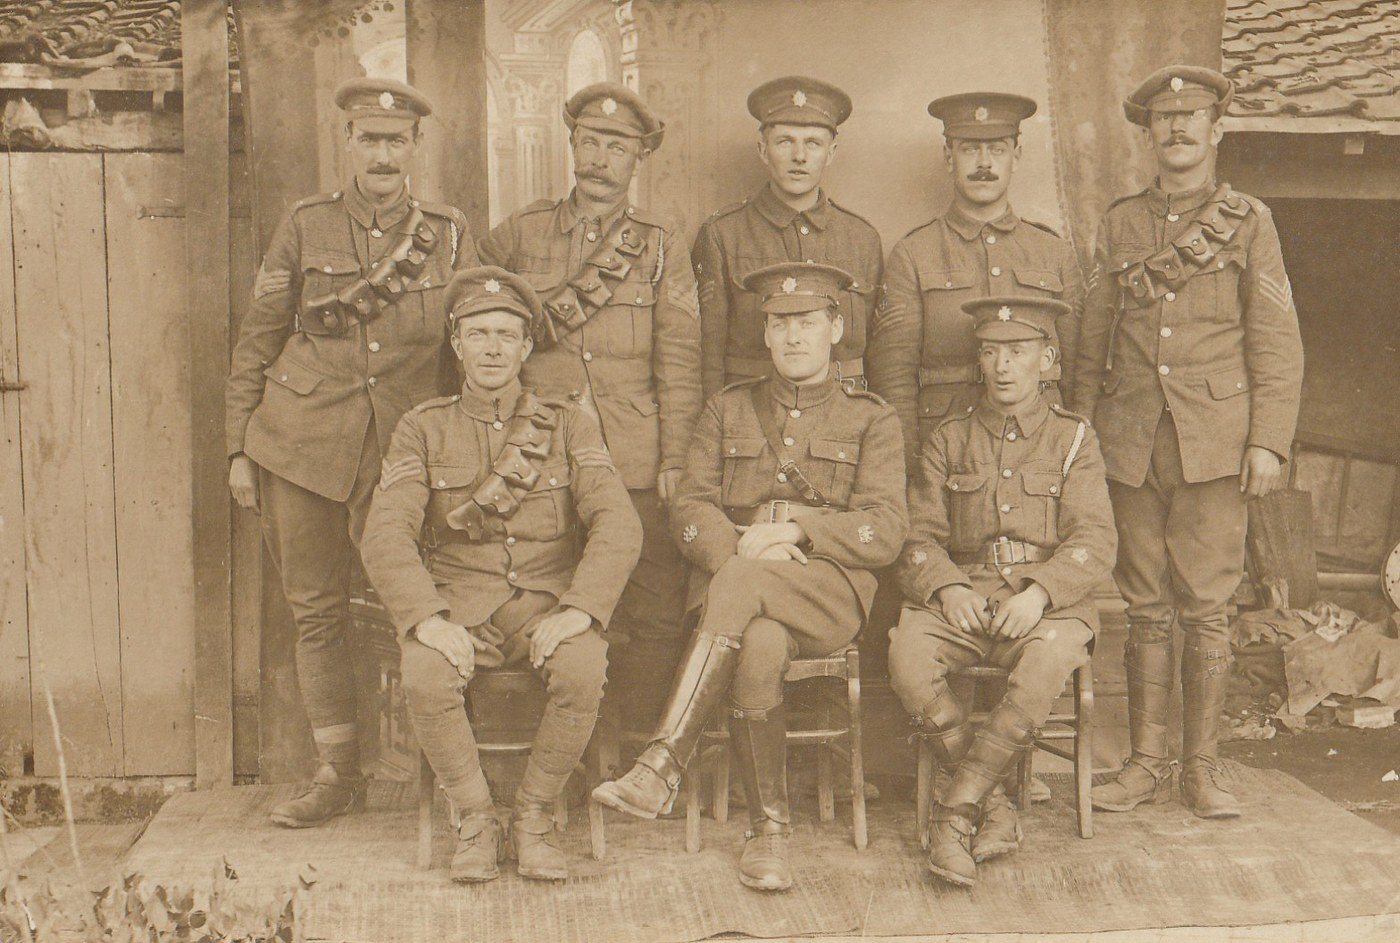
\includegraphics[width=0.94\linewidth,height=22mm,keepaspectratio]{illustrations/camarades_ailly_1919.jpg}}
    \par\vspace{0.6mm}{\fontsize{5.8pt}{6.7pt}\selectfont Souvenir de camaraderie militaire sur le front de Picardie (carte-photo dédicacée à Hippolyte Combes, Ailly-sur-Noye, mai 1919). Collection familiale.}
  \end{minipage}
\end{center}
\clearpage

% =============================================================================
% VIS-A-VIS SPREAD : SCAN #105 (20251126_104946.jpg) — Vue 105
% =============================================================================
\cleardoubleevenpage
% --- En-tête du folio (Page paire / gauche : Transcription, apparat & double registre) ---
\noindent\rule{\textwidth}{0.5pt}\par\vspace{0.6mm}
\noindent\textbf{\footnotesize SCAN \#105 — VUE 105} \hfill {\scriptsize\texttt{20251126\_\allowbreak 104946.jpg}}\par\vspace{0.3mm}
\noindent{\fontsize{7.0pt}{8.2pt}\selectfont Tournée à Franvillers et Buire-sur-l'Ancre, arrivée imprévue du très jeune capitaine Williams}\par\vspace{0.25mm}
\noindent{\fontsize{7.0pt}{8.2pt}\selectfont\textit{1er – 2 décembre 1916} \hfill \textit{Acheux, Franvillers, Buire-sur-l'Ancre, Ribemont, Heilly, Toutencourt (Somme)}}\par\vspace{0.6mm}
\noindent\rule{\textwidth}{0.35pt}\par\vspace{1.0mm}
% --- Corps de la transcription diplomatique et apparat marginal en prolongement ---
{\renewcommand{\arraystretch}{0.89}%
\noindent\hspace*{3.5mm}\begin{tabular}{@{}p{100mm}@{\hspace{3.5mm}}p{55mm}@{}}
      \leavevmode\fontsize{7.0pt}{8.1pt}\selectfont\strut 1er Ven. \hfill{} Décembre 1916\strut & \leavevmode\fontsize{6.3pt}{7.2pt}\selectfont\raggedright\arraybackslash\color{black!88}\textbf{1} \textbf{Ven.} \textit{vendredi}. \\
      \leavevmode\fontsize{7.0pt}{8.1pt}\selectfont\strut Matinée perdue à ne rien faire : office \& billet.\strut & \leavevmode\fontsize{6.3pt}{7.2pt}\selectfont\raggedright\arraybackslash\color{black!88}\textbf{2} \textbf{office} \textit{angl.} bureau militaire ; \textbf{billet} \textit{angl.} cantonnement, logement attribué. \\
      \leavevmode\fontsize{7.0pt}{8.1pt}\selectfont\strut Après early lunch, partis en auto. Venus\strut & \leavevmode\fontsize{6.3pt}{7.2pt}\selectfont\raggedright\arraybackslash\color{black!88}\textbf{3} \textbf{early lunch} \textit{angl.} repas de midi pris tôt. \\
      \leavevmode\fontsize{7.0pt}{8.1pt}\selectfont\strut à Franvillers, puis à Buire s/ Ancre pour\strut & \leavevmode\fontsize{6.3pt}{7.2pt}\selectfont\raggedright\arraybackslash\color{black!88}\textbf{4} \textbf{s/} \textit{sur}. \\
      \leavevmode\llap{\fontsize{6.5pt}{7.5pt}\selectfont\color{darkgray}5\hspace{1.8mm}}\fontsize{7.0pt}{8.1pt}\selectfont\strut affaires à traiter.\strut &  \\
      \leavevmode\fontsize{7.0pt}{8.1pt}\selectfont\strut Plaisir à revoir région de Ribemont – Heilly.\strut &  \\
      \leavevmode\fontsize{7.0pt}{8.1pt}\selectfont\strut Au retour, arrêté à Toutencourt \& monté\strut &  \\
      \leavevmode\fontsize{7.0pt}{8.1pt}\selectfont\strut bureau mission frse, Ve armée, Cap. Bresson.\strut & \leavevmode\fontsize{6.3pt}{7.2pt}\selectfont\raggedright\arraybackslash\color{black!88}\textbf{8} \textbf{frse} \textit{française} ; \textbf{Cap.} \textit{capitaine}. \\
      \leavevmode\fontsize{7.0pt}{8.1pt}\selectfont\strut Trouvé message à Acheux — présenté au\strut &  \\
      \leavevmode\llap{\fontsize{6.5pt}{7.5pt}\selectfont\color{darkgray}10\hspace{1.8mm}}\fontsize{7.0pt}{8.1pt}\selectfont\strut bureau M.F., XIIIe corps et pris en charge.\strut & \leavevmode\fontsize{6.3pt}{7.2pt}\selectfont\raggedright\arraybackslash\color{black!88}\textbf{10} \textbf{M.F.} \textit{Mission française, dans ce contexte}. \\
      \leavevmode\fontsize{7.0pt}{8.1pt}\selectfont\strut Perspective réintégration prochaine ds\strut & \leavevmode\fontsize{6.3pt}{7.2pt}\selectfont\raggedright\arraybackslash\color{black!88}\textbf{11} \textbf{ds} \textit{dans}. \\
      \leavevmode\fontsize{7.0pt}{8.1pt}\selectfont\strut régiment d'origine! —\strut &  \\
      \leavevmode\fontsize{7.0pt}{8.1pt}\selectfont\strut [ — A Curtis, pour ma part de\strut & \leavevmode\fontsize{6.3pt}{7.2pt}\selectfont\raggedright\arraybackslash\color{black!88}\textbf{13} \textbf{[ — A Curtis} début du compte, crochet gauche autographe dans le corps de la page. \\
      \leavevmode\fontsize{7.0pt}{8.1pt}\selectfont\strut dépenses du mess, à Acheux : 40 f\strut & \leavevmode\fontsize{6.3pt}{7.2pt}\selectfont\raggedright\arraybackslash\color{black!88}\textbf{14} \textbf{mess} \textit{angl.} repas ou table commune des officiers. \\
      \leavevmode\llap{\fontsize{6.5pt}{7.5pt}\selectfont\color{darkgray}15\hspace{1.8mm}}\fontsize{7.0pt}{8.1pt}\selectfont\strut (novembre) | Tin of black\strut & \leavevmode\fontsize{6.3pt}{7.2pt}\selectfont\raggedright\arraybackslash\color{black!88}\textbf{15} \textbf{Tin of black} \textit{angl.} début d’un libellé anglais : boîte de cirage noir ; suite à la ligne suivante. \\
      \leavevmode\fontsize{7.0pt}{8.1pt}\selectfont\strut (Nugget) boot polish : 30 c ]\strut & \leavevmode\fontsize{6.3pt}{7.2pt}\selectfont\raggedright\arraybackslash\color{black!88}\textbf{16} \textbf{(Nugget) boot polish} \textit{angl.} cirage pour chaussures, marque Nugget ; suite du libellé précédent. \\
      \leavevmode\fontsize{7.0pt}{8.1pt}\selectfont\strut 2 Samedi.\strut &  \\
      \leavevmode\fontsize{7.0pt}{8.1pt}\selectfont\strut Nuit, gelé très fortt. Temps sec \& froid.\strut & \leavevmode\fontsize{6.3pt}{7.2pt}\selectfont\raggedright\arraybackslash\color{black!88}\textbf{18} \textbf{fortt} \textit{fortement}. \\
      \leavevmode\fontsize{7.0pt}{8.1pt}\selectfont\strut Pas de bise.\strut &  \\
      \leavevmode\llap{\fontsize{6.5pt}{7.5pt}\selectfont\color{darkgray}20\hspace{1.8mm}}\fontsize{7.0pt}{8.1pt}\selectfont\strut Tout le jour, resté à Acheux.\strut &  \\
      \leavevmode\fontsize{7.0pt}{8.1pt}\selectfont\strut Vers 4h après-midi, Cap. Williams, arrivé tout\strut & \leavevmode\fontsize{6.3pt}{7.2pt}\selectfont\raggedright\arraybackslash\color{black!88}\textbf{21} \textbf{Cap.} \textit{capitaine}. \\
      \leavevmode\fontsize{7.0pt}{8.1pt}\selectfont\strut jeune, mince. Il vient remplacer Lt Curtis. Étonnement profond.\strut & \leavevmode\fontsize{6.3pt}{7.2pt}\selectfont\raggedright\arraybackslash\color{black!88}\textbf{22} \textbf{Lt} \textit{lieutenant}. \\
      \leavevmode\fontsize{7.0pt}{8.1pt}\selectfont\strut Curtis, à Martinsart. A son retour, tant\strut &  \\
      \leavevmode\fontsize{7.0pt}{8.1pt}\selectfont\strut surpris : visibt découragé — que faire?\strut & \leavevmode\fontsize{6.3pt}{7.2pt}\selectfont\raggedright\arraybackslash\color{black!88}\textbf{24} \textbf{visibt} \textit{visiblement}. \\
      \leavevmode\llap{\fontsize{6.5pt}{7.5pt}\selectfont\color{darkgray}25\hspace{1.8mm}}\fontsize{7.0pt}{8.1pt}\selectfont\strut Soir, venu au bureau mission \&\strut &  \\
      \leavevmode\fontsize{7.0pt}{8.1pt}\selectfont\strut vu Cap. H.\strut & \leavevmode\fontsize{6.3pt}{7.2pt}\selectfont\raggedright\arraybackslash\color{black!88}\textbf{26} \textbf{Cap. H.} \textit{capitaine H. ; prénom ou patronyme non développé}. \\
\end{tabular}}%
\par\vspace*{\fill}
% --- Deux registres de commentaires en bas de page (sans intitulés, distingués par filets et mise en page) ---
\noindent\rule{\textwidth}{0.5pt}\par\vspace{0.8mm}
{\fontsize{6.8pt}{8.0pt}\selectfont%
\noindent\normalfont Lignes 2–3 : office et billet sont employés dans le sens britannique de bureau et logement ; early lunch désigne un repas de midi pris tôt. Lignes 13–16 : le compte occupe quatre lignes du corps de page, introduites par un crochet gauche. L’anglais Tin of black / (Nugget) boot polish est réparti sur deux lignes : boîte de cirage noir, Nugget ; sa disposition ne doit pas devenir deux achats. Ligne 26 : seule l’initiale H. est écrite après le grade ; aucun nom complet n’est rétabli.\par\vspace{0.75mm}
\noindent\rule{38mm}{0.4pt}\par\vspace{0.65mm}
\noindent\hspace*{5mm}\parbox{\dimexpr\textwidth-5mm\relax}{\fontsize{6.8pt}{8.0pt}\selectfont\color{black!82}\textbf{Bureaux et remplacement :} Le 1er décembre, la tournée vers Franvillers et Buire-sur-Ancre lui fait revoir la région de Ribemont--Heilly. Les mentions de la Mission française à Toutencourt (Ve Armée, Bresson) puis à Acheux (XIIIe Corps) sont conservées. Cap. H. peut être rapproché de Huguet, nommé ailleurs, sans développer automatiquement cette initiale. Le 2 décembre, Williams arrive pour remplacer Curtis; la page décrit leur réaction, sans donner les conditions administratives de la nomination.}\par}
\newpage
% --- En-tête du fac-similé (Page impaire / droite : Scan original) ---
\noindent\rule{\textwidth}{0.5pt}\par\vspace{0.6mm}
\noindent\textbf{\fontsize{6.5pt}{7.6pt}\selectfont FAC-SIMILÉ EN VIS-À-VIS — VUE 105 (SCAN \#105)} \hfill {\fontsize{6.5pt}{7.6pt}\selectfont\texttt{20251126\_\allowbreak 104946.jpg}}\par\vspace{0.3mm}
\noindent{\fontsize{6.8pt}{8pt}\selectfont\textit{Livre-Journal d'Hippolyte Combes} — 1er – 2 décembre 1916 (Acheux, Franvillers, Buire-sur-l'Ancre, Ribemont, Heilly, Toutencourt (Somme))}\par\vspace{0.6mm}
\noindent\rule{\textwidth}{0.35pt}\par\vspace*{\fill}
{\centering
  \setlength{\fboxsep}{1.2mm}%
  \setlength{\fboxrule}{0.4pt}%
  \fcolorbox{gray!55}{white}{%
    \includegraphics[width=0.94\textwidth,height=0.76\textheight,keepaspectratio]{\facsimiledir/20251126_104946.jpg}%
  }\par}
\vspace*{\fill}
\noindent\rule{\textwidth}{0.35pt}\par\vspace{0.5mm}
\noindent{\fontsize{6pt}{7.1pt}\selectfont\raggedright\color{darkgray}\textbf{Source :} Archives familiales Combes — Cliché numérique \texttt{20251126\_\allowbreak 104946.jpg} (Scan \#105/186, Vue 105). Haute définition : \texttt{scans\_haute\_qualite/\allowbreak 20251126\_\allowbreak 104946.jpg} ; version allégée : \texttt{scans\_compresses/\allowbreak 20251126\_\allowbreak 104946.jpg}.\par}
\newpage

% =============================================================================
% VIS-A-VIS SPREAD : SCAN #106 (20251126_105005.jpg) — Vue 106
% =============================================================================
\cleardoubleevenpage
% --- En-tête du folio (Page paire / gauche : Transcription, apparat & double registre) ---
\noindent\rule{\textwidth}{0.5pt}\par\vspace{0.6mm}
\noindent\textbf{\footnotesize SCAN \#106 — VUE 106} \hfill {\scriptsize\texttt{20251126\_\allowbreak 105005.jpg}}\par\vspace{0.3mm}
\noindent{\fontsize{7.0pt}{8.2pt}\selectfont Longue randonnée jusqu'à Corbie, Villers-Bretonneux et Marcelcave dans la brume glaciale}\par\vspace{0.25mm}
\noindent{\fontsize{7.0pt}{8.2pt}\selectfont\textit{3 – 4 décembre 1916} \hfill \textit{Acheux, Septenville, Hérissart, Corbie, Villers-Bretonneux, Marcelcave, Warfusée-Abancourt, Arquèves, Louvencourt (Somme)}}\par\vspace{0.6mm}
\noindent\rule{\textwidth}{0.35pt}\par\vspace{1.0mm}
% --- Corps de la transcription diplomatique et apparat marginal en prolongement ---
{\renewcommand{\arraystretch}{0.89}%
\noindent\hspace*{3.5mm}\begin{tabular}{@{}p{100mm}@{\hspace{3.5mm}}p{55mm}@{}}
      \leavevmode\fontsize{7.0pt}{8.1pt}\selectfont\strut 3 Dim. — \hfill{} Décbre 1916\strut & \leavevmode\fontsize{6.3pt}{7.2pt}\selectfont\raggedright\arraybackslash\color{black!88}\textbf{1} \textbf{Dim.} \textit{dimanche} ; \textbf{Décbre} \textit{décembre}. \\
      \leavevmode\fontsize{7.0pt}{8.1pt}\selectfont\strut Nuit très froide. Gelé 1 peu moins que nuit\strut &  \\
      \leavevmode\fontsize{7.0pt}{8.1pt}\selectfont\strut précédente.\strut &  \\
      \leavevmode\fontsize{7.0pt}{8.1pt}\selectfont\strut Journée bien remplie \& fatigante. Partis vers\strut &  \\
      \leavevmode\llap{\fontsize{6.5pt}{7.5pt}\selectfont\color{darkgray}5\hspace{1.8mm}}\fontsize{7.0pt}{8.1pt}\selectfont\strut 8h 1/2 m. et rentrés seulement à 6h 1/2 s.\strut &  \\
      \leavevmode\fontsize{7.0pt}{8.1pt}\selectfont\strut Longues courses en auto, matin \& soir :\strut &  \\
      \leavevmode\fontsize{7.0pt}{8.1pt}\selectfont\strut Septenville et Hérissart. Déjeuné ch. Lieutt Walsh.\strut & \leavevmode\fontsize{6.3pt}{7.2pt}\selectfont\raggedright\arraybackslash\color{black!88}\textbf{7} \textbf{ch.} \textit{chez} ; \textbf{Lieutt} \textit{lieutenant}. \\
      \leavevmode\fontsize{7.0pt}{8.1pt}\selectfont\strut Après lunch, venus j'à Marcelcave. Passé\strut & \leavevmode\fontsize{6.3pt}{7.2pt}\selectfont\raggedright\arraybackslash\color{black!88}\textbf{8} \textbf{lunch} \textit{angl.} repas de midi ; \textbf{j'à} \textit{jusqu’à}. \\
      \leavevmode\fontsize{7.0pt}{8.1pt}\selectfont\strut à Corbie et Villers-Bretonneux.\strut &  \\
      \leavevmode\llap{\fontsize{6.5pt}{7.5pt}\selectfont\color{darkgray}10\hspace{1.8mm}}\fontsize{7.0pt}{8.1pt}\selectfont\strut Retour par Warfusée-Abancourt.\strut &  \\
      \leavevmode\fontsize{7.0pt}{8.1pt}\selectfont\strut Tt jour, brume glaciale enveloppé choses.\strut & \leavevmode\fontsize{6.3pt}{7.2pt}\selectfont\raggedright\arraybackslash\color{black!88}\textbf{11} \textbf{Tt} \textit{Tout}. \\
      \leavevmode\fontsize{7.0pt}{8.1pt}\selectfont\strut Moulins squelettiques au 1/2 des champs...\strut & \leavevmode\fontsize{6.3pt}{7.2pt}\selectfont\raggedright\arraybackslash\color{black!88}\textbf{12} \textbf{1/2} milieu, dans « au milieu des champs ». \\
      \leavevmode\fontsize{7.0pt}{8.1pt}\selectfont\strut Heures mornes en auto : pu ruminer \&\strut &  \\
      \leavevmode\fontsize{7.0pt}{8.1pt}\selectfont\strut observer à loisir...\strut &  \\
      \leavevmode\llap{\fontsize{6.5pt}{7.5pt}\selectfont\color{darkgray}15\hspace{1.8mm}}\fontsize{7.0pt}{8.1pt}\selectfont\strut [ — A Hérissart, 2 bocks : 30 c\strut & \leavevmode\fontsize{6.3pt}{7.2pt}\selectfont\raggedright\arraybackslash\color{black!88}\textbf{15} \textbf{[ — A Hérissart} début du bloc de comptes, crochet gauche autographe. \\
      \leavevmode\fontsize{7.0pt}{8.1pt}\selectfont\strut Au bureau mission XIIIe corps, Acheux,\strut &  \\
      \leavevmode\fontsize{7.0pt}{8.1pt}\selectfont\strut touché solde : 78 f 75 c (prochaine, le 17) ]\strut &  \\
      \leavevmode\fontsize{7.0pt}{8.1pt}\selectfont\strut 4 L. Matinée, dégelé rapidt et\strut & \leavevmode\fontsize{6.3pt}{7.2pt}\selectfont\raggedright\arraybackslash\color{black!88}\textbf{18} \textbf{L.} \textit{lundi} ; \textbf{rapidt} \textit{rapidement}. \\
      \leavevmode\fontsize{7.0pt}{8.1pt}\selectfont\strut routes redevenues boueuses.\strut &  \\
      \leavevmode\llap{\fontsize{6.5pt}{7.5pt}\selectfont\color{darkgray}20\hspace{1.8mm}}\fontsize{7.0pt}{8.1pt}\selectfont\strut Tout le matin, ds la grange de Mme Guerle,\strut & \leavevmode\fontsize{6.3pt}{7.2pt}\selectfont\raggedright\arraybackslash\color{black!88}\textbf{20} \textbf{ds} \textit{dans} ; \textbf{Mme} \textit{Madame}. \\
      \leavevmode\fontsize{7.0pt}{8.1pt}\selectfont\strut soleil brillé 1 peu —\strut &  \\
      \leavevmode\fontsize{7.0pt}{8.1pt}\selectfont\strut Après-midi, courses en auto à\strut &  \\
      \leavevmode\fontsize{7.0pt}{8.1pt}\selectfont\strut ferme de Belle-Église (Arquèves) et à Louvencourt.\strut &  \\
      \leavevmode\fontsize{7.0pt}{8.1pt}\selectfont\strut Rentré pour le thé et dès lors liberté.\strut &  \\
      \leavevmode\llap{\fontsize{6.5pt}{7.5pt}\selectfont\color{darkgray}25\hspace{1.8mm}}\fontsize{7.0pt}{8.1pt}\selectfont\strut Lt Walsh \& son interprète, invités à dîner.\strut & \leavevmode\fontsize{6.3pt}{7.2pt}\selectfont\raggedright\arraybackslash\color{black!88}\textbf{25} \textbf{Lt} \textit{lieutenant}. \\
      \leavevmode\fontsize{7.0pt}{8.1pt}\selectfont\strut Capt. Williams, charmant et de tt à tt sympathique.\strut & \leavevmode\fontsize{6.3pt}{7.2pt}\selectfont\raggedright\arraybackslash\color{black!88}\textbf{26} \textbf{Capt.} \textit{captain, capitaine} ; \textbf{de tt à tt} \textit{de tout à tout ; expression telle qu’écrite}. \\
\end{tabular}}%
\par\vspace*{\fill}
% --- Deux registres de commentaires en bas de page (sans intitulés, distingués par filets et mise en page) ---
\noindent\rule{\textwidth}{0.5pt}\par\vspace{0.8mm}
{\fontsize{6.8pt}{8.0pt}\selectfont%
\noindent\normalfont Ligne 12 : au 1/2 des champs signifie au milieu des champs. Lignes 15–17 : le compte, à gauche duquel Combes trace un crochet, occupe le corps de page ; 2 bocks est le libellé écrit. Ligne 26 : de tt à tt se développe de tout à tout, expression conservée sans la remplacer par de tout au tout. Capt. est la contraction du grade anglais captain, ici capitaine.\par\vspace{0.75mm}
\noindent\rule{38mm}{0.4pt}\par\vspace{0.65mm}
\noindent\hspace*{5mm}\parbox{\dimexpr\textwidth-5mm\relax}{\fontsize{6.8pt}{8.0pt}\selectfont\color{black!82}\textbf{Tournées et versement :} Le 3 décembre, courses vers Septenville et Hérissart, puis Marcelcave par Corbie et Villers-Bretonneux, retour par Warfusée-Abancourt. Le compte porte 78 f 75 et annonce le prochain versement le 17, sans expliciter une règle de quinzaine. Le 4, courses vers Belle-Église et Louvencourt; Williams paraît alors charmant et sympathique à Combes, appréciation qu’il faut conserver à sa date.}\par}
\newpage
% --- En-tête du fac-similé (Page impaire / droite : Scan original) ---
\noindent\rule{\textwidth}{0.5pt}\par\vspace{0.6mm}
\noindent\textbf{\fontsize{6.5pt}{7.6pt}\selectfont FAC-SIMILÉ EN VIS-À-VIS — VUE 106 (SCAN \#106)} \hfill {\fontsize{6.5pt}{7.6pt}\selectfont\texttt{20251126\_\allowbreak 105005.jpg}}\par\vspace{0.3mm}
\noindent{\fontsize{6.8pt}{8pt}\selectfont\textit{Livre-Journal d'Hippolyte Combes} — 3 – 4 décembre 1916 (Acheux, Septenville, Hérissart, Corbie, Villers-Bretonneux, Marcelcave, Warfusée-Abancourt, Arquèves, Louvencourt (Somme))}\par\vspace{0.6mm}
\noindent\rule{\textwidth}{0.35pt}\par\vspace*{\fill}
{\centering
  \setlength{\fboxsep}{1.2mm}%
  \setlength{\fboxrule}{0.4pt}%
  \fcolorbox{gray!55}{white}{%
    \includegraphics[width=0.94\textwidth,height=0.76\textheight,keepaspectratio]{\facsimiledir/20251126_105005.jpg}%
  }\par}
\vspace*{\fill}
\noindent\rule{\textwidth}{0.35pt}\par\vspace{0.5mm}
\noindent{\fontsize{6pt}{7.1pt}\selectfont\raggedright\color{darkgray}\textbf{Source :} Archives familiales Combes — Cliché numérique \texttt{20251126\_\allowbreak 105005.jpg} (Scan \#106/186, Vue 106). Haute définition : \texttt{scans\_haute\_qualite/\allowbreak 20251126\_\allowbreak 105005.jpg} ; version allégée : \texttt{scans\_compresses/\allowbreak 20251126\_\allowbreak 105005.jpg}.\par}
\newpage

% =============================================================================
% VIS-A-VIS SPREAD : SCAN #107 (20251126_105017.jpg) — Vue 107
% =============================================================================
\cleardoubleevenpage
% --- En-tête du folio (Page paire / gauche : Transcription, apparat & double registre) ---
\noindent\rule{\textwidth}{0.5pt}\par\vspace{0.6mm}
\noindent\textbf{\footnotesize SCAN \#107 — VUE 107} \hfill {\scriptsize\texttt{20251126\_\allowbreak 105017.jpg}}\par\vspace{0.3mm}
\noindent{\fontsize{7.0pt}{8.2pt}\selectfont Course jusqu'aux ruines de Bayencourt et Coigneux, départ de Curtis et confidences de Williams}\par\vspace{0.25mm}
\noindent{\fontsize{7.0pt}{8.2pt}\selectfont\textit{5 – 6 décembre 1916} \hfill \textit{Acheux, Authie, Bayencourt, Coigneux, Louvencourt, Raincheval (Somme / Pas-de-Calais)}}\par\vspace{0.6mm}
\noindent\rule{\textwidth}{0.35pt}\par\vspace{1.0mm}
% --- Corps de la transcription diplomatique et apparat marginal en prolongement ---
{\renewcommand{\arraystretch}{1.02}%
\noindent\hspace*{3.5mm}\begin{tabular}{@{}p{100mm}@{\hspace{3.5mm}}p{55mm}@{}}
      \leavevmode\fontsize{7.8pt}{9.2pt}\selectfont\strut 5 Mardi. \hfill{} Décbre 1916\strut & \leavevmode\fontsize{6.3pt}{7.2pt}\selectfont\raggedright\arraybackslash\color{black!88}\textbf{1} \textbf{Décbre} \textit{décembre}. \\
      \leavevmode\fontsize{7.8pt}{9.2pt}\selectfont\strut Matinée, liberté complète.\strut &  \\
      \leavevmode\fontsize{7.8pt}{9.2pt}\selectfont\strut Après-midi, course à Authie, puis à\strut &  \\
      \leavevmode\fontsize{7.8pt}{9.2pt}\selectfont\strut Bayencourt, près d'Hébuterne, à 3 kilomètres\strut &  \\
      \leavevmode\llap{\fontsize{6.5pt}{7.5pt}\selectfont\color{darkgray}5\hspace{1.8mm}}\fontsize{7.8pt}{9.2pt}\selectfont\strut de Gommecourt (Boches). Dépassé le village. Champs\strut &  \\
      \leavevmode\fontsize{7.8pt}{9.2pt}\selectfont\strut dévastés. Obus non éclatés... Village de Coigneux,\strut &  \\
      \leavevmode\fontsize{7.8pt}{9.2pt}\selectfont\strut bp de toits squelettiques, + de tuiles, à la\strut & \leavevmode\fontsize{6.3pt}{7.2pt}\selectfont\raggedright\arraybackslash\color{black!88}\textbf{7} \textbf{bp} \textit{beaucoup} ; \textbf{+ de tuiles} plus de tuiles : les tuiles ont disparu. \\
      \leavevmode\fontsize{7.8pt}{9.2pt}\selectfont\strut suite de bombardement.\strut &  \\
      \leavevmode\fontsize{7.8pt}{9.2pt}\selectfont\strut Brume épaisse et, par moments, pluie\strut &  \\
      \leavevmode\llap{\fontsize{6.5pt}{7.5pt}\selectfont\color{darkgray}10\hspace{1.8mm}}\fontsize{7.8pt}{9.2pt}\selectfont\strut fine. Après dîner, adieux avec Lieutt\strut & \leavevmode\fontsize{6.3pt}{7.2pt}\selectfont\raggedright\arraybackslash\color{black!88}\textbf{10} \textbf{Lieutt} \textit{lieutenant}. \\
      \leavevmode\fontsize{7.8pt}{9.2pt}\selectfont\strut Curtis qui doit repartir, demain matin, pour\strut &  \\
      \leavevmode\fontsize{7.8pt}{9.2pt}\selectfont\strut rejoindre la 152 Coy A.S.C.\strut & \leavevmode\fontsize{6.3pt}{7.2pt}\selectfont\raggedright\arraybackslash\color{black!88}\textbf{12} \textbf{Coy} \textit{company, compagnie britannique} ; \textbf{A.S.C.} \textit{Army Service Corps, corps britannique du ravitaillement et des transports}. \\
      \leavevmode\fontsize{7.8pt}{9.2pt}\selectfont\strut 6 Merc. Levé 6h m. — Lt Curtis, parti vers\strut & \leavevmode\fontsize{6.3pt}{7.2pt}\selectfont\raggedright\arraybackslash\color{black!88}\textbf{13} \textbf{Merc.} \textit{mercredi} ; \textbf{Lt} \textit{lieutenant}. \\
      \leavevmode\fontsize{7.8pt}{9.2pt}\selectfont\strut 7h 1/2 m. — \& sans laisser de regret — A brainless\strut & \leavevmode\fontsize{6.3pt}{7.2pt}\selectfont\raggedright\arraybackslash\color{black!88}\textbf{14} \textbf{A brainless} \textit{angl.} début de l’injure anglaise, un âne sans cervelle ; suite ass à la ligne suivante. \\
      \leavevmode\llap{\fontsize{6.5pt}{7.5pt}\selectfont\color{darkgray}15\hspace{1.8mm}}\fontsize{7.8pt}{9.2pt}\selectfont\strut ass. Matin, course à Louvencourt, Raincheval\strut & \leavevmode\fontsize{6.3pt}{7.2pt}\selectfont\raggedright\arraybackslash\color{black!88}\textbf{15} \textbf{ass.} \textit{angl.} âne, dans A brainless ass ; injure visant Curtis. \\
      \leavevmode\fontsize{7.8pt}{9.2pt}\selectfont\strut etc.\strut &  \\
      \leavevmode\fontsize{7.8pt}{9.2pt}\selectfont\strut Nouvel off., Cap. Williams, 20 ans! Après\strut & \leavevmode\fontsize{6.3pt}{7.2pt}\selectfont\raggedright\arraybackslash\color{black!88}\textbf{17} \textbf{off.} \textit{officier} ; \textbf{Cap.} \textit{capitaine}. \\
      \leavevmode\fontsize{7.8pt}{9.2pt}\selectfont\strut repas soir, s'est 1 peu raconté : avant\strut &  \\
      \leavevmode\fontsize{7.8pt}{9.2pt}\selectfont\strut la guerre, était office boy à 50 £ a year.\strut & \leavevmode\fontsize{6.3pt}{7.2pt}\selectfont\raggedright\arraybackslash\color{black!88}\textbf{19} \textbf{office boy} \textit{angl.} jeune employé de bureau ; \textbf{a year} \textit{angl.} par an. \\
\end{tabular}}%
\par\vspace*{\fill}
% --- Deux registres de commentaires en bas de page (sans intitulés, distingués par filets et mise en page) ---
\noindent\rule{\textwidth}{0.5pt}\par\vspace{0.8mm}
{\fontsize{6.8pt}{8.0pt}\selectfont%
\noindent\normalfont Ligne 7 : + de tuiles signifie ici plus de tuiles, au sens de disparition des couvertures, après la mention des toits squelettiques ; ce n’est pas une quantité accrue. Lignes 14–15 : A brainless ass est l’injure formulée par le diariste à propos de Curtis, « un âne sans cervelle » ; aucune citation attribuée à un tiers n’est indiquée. Ligne 19 : office boy désigne un jeune employé de bureau ; a year signifie par an, la somme étant exprimée en livres sterling. Ces indications ne suffisent pas à reconstruire une carrière.\par\vspace{0.75mm}
\noindent\rule{38mm}{0.4pt}\par\vspace{0.65mm}
\noindent\hspace*{5mm}\parbox{\dimexpr\textwidth-5mm\relax}{\fontsize{6.8pt}{8.0pt}\selectfont\color{black!82}\textbf{Départ de Curtis :} La course du 5 décembre atteint Authie, Bayencourt et Coigneux, avec Hébuterne et Gommecourt comme repères manuscrits. Le 6, Curtis repart pour la 152 Coy A.S.C. ; Combes le juge durement en anglais. Williams, âgé de 20 ans selon le carnet, raconte avoir été office boy à 50 livres annuelles avant la guerre. Ni carrière détaillée ni causes de sa promotion ne sont données.}\par}
\newpage
% --- En-tête du fac-similé (Page impaire / droite : Scan original) ---
\noindent\rule{\textwidth}{0.5pt}\par\vspace{0.6mm}
\noindent\textbf{\fontsize{6.5pt}{7.6pt}\selectfont FAC-SIMILÉ EN VIS-À-VIS — VUE 107 (SCAN \#107)} \hfill {\fontsize{6.5pt}{7.6pt}\selectfont\texttt{20251126\_\allowbreak 105017.jpg}}\par\vspace{0.3mm}
\noindent{\fontsize{6.8pt}{8pt}\selectfont\textit{Livre-Journal d'Hippolyte Combes} — 5 – 6 décembre 1916 (Acheux, Authie, Bayencourt, Coigneux, Louvencourt, Raincheval (Somme / Pas-de-Calais))}\par\vspace{0.6mm}
\noindent\rule{\textwidth}{0.35pt}\par\vspace*{\fill}
{\centering
  \setlength{\fboxsep}{1.2mm}%
  \setlength{\fboxrule}{0.4pt}%
  \fcolorbox{gray!55}{white}{%
    \includegraphics[width=0.94\textwidth,height=0.76\textheight,keepaspectratio]{\facsimiledir/20251126_105017.jpg}%
  }\par}
\vspace*{\fill}
\noindent\rule{\textwidth}{0.35pt}\par\vspace{0.5mm}
\noindent{\fontsize{6pt}{7.1pt}\selectfont\raggedright\color{darkgray}\textbf{Source :} Archives familiales Combes — Cliché numérique \texttt{20251126\_\allowbreak 105017.jpg} (Scan \#107/186, Vue 107). Haute définition : \texttt{scans\_haute\_qualite/\allowbreak 20251126\_\allowbreak 105017.jpg} ; version allégée : \texttt{scans\_compresses/\allowbreak 20251126\_\allowbreak 105017.jpg}.\par}
\newpage

% =============================================================================
% VIS-A-VIS SPREAD : SCAN #108 (20251126_105046.jpg) — Vue 108
% =============================================================================
\cleardoubleevenpage
% --- En-tête du folio (Page paire / gauche : Transcription, apparat & double registre) ---
\noindent\rule{\textwidth}{0.5pt}\par\vspace{0.6mm}
\noindent\textbf{\footnotesize SCAN \#108 — VUE 108} \hfill {\scriptsize\texttt{20251126\_\allowbreak 105046.jpg}}\par\vspace{0.3mm}
\noindent{\fontsize{7.0pt}{8.2pt}\selectfont Les enfants de la fermière belge de Belle-Église et le village désert d'Englebelmer}\par\vspace{0.25mm}
\noindent{\fontsize{7.0pt}{8.2pt}\selectfont\textit{7 – 8 décembre 1916} \hfill \textit{Acheux, Arquèves (Belle-Église), Hédauville, Englebelmer, Saint-Léger-lès-Authie (Somme)}}\par\vspace{0.6mm}
\noindent\rule{\textwidth}{0.35pt}\par\vspace{1.0mm}
% --- Corps de la transcription diplomatique et apparat marginal en prolongement ---
{\renewcommand{\arraystretch}{0.89}%
\noindent\hspace*{3.5mm}\begin{tabular}{@{}p{100mm}@{\hspace{3.5mm}}p{55mm}@{}}
      \leavevmode\fontsize{7.0pt}{8.1pt}\selectfont\strut 7 Jeudi — — Décbre 1916 —\strut & \leavevmode\fontsize{6.3pt}{7.2pt}\selectfont\raggedright\arraybackslash\color{black!88}\textbf{1} \textbf{Décbre} \textit{décembre}. \\
      \leavevmode\fontsize{7.0pt}{8.1pt}\selectfont\strut Matin \& après-midi, en\strut &  \\
      \leavevmode\fontsize{7.0pt}{8.1pt}\selectfont\strut auto. — Matin, à Belle-Église, Arquèves,\strut &  \\
      \leavevmode\fontsize{7.0pt}{8.1pt}\selectfont\strut où dû attendre lgts retour du Cap. W.,\strut & \leavevmode\fontsize{6.3pt}{7.2pt}\selectfont\raggedright\arraybackslash\color{black!88}\textbf{4} \textbf{lgts} \textit{longtemps} ; \textbf{Cap. W.} \textit{capitaine W., probablement Williams, nommé dans les entrées voisines}. \\
      \leavevmode\llap{\fontsize{6.5pt}{7.5pt}\selectfont\color{darkgray}5\hspace{1.8mm}}\fontsize{7.0pt}{8.1pt}\selectfont\strut qui allé j'à Raincheval. Amusé par les\strut & \leavevmode\fontsize{6.3pt}{7.2pt}\selectfont\raggedright\arraybackslash\color{black!88}\textbf{5} \textbf{j'à} \textit{jusqu’à}. \\
      \leavevmode\fontsize{7.0pt}{8.1pt}\selectfont\strut enfants de la fermière belge, Mme Houtteman [?].\strut & \leavevmode\fontsize{6.3pt}{7.2pt}\selectfont\raggedright\arraybackslash\color{black!88}\textbf{6} \textbf{Mme} \textit{Madame} ; \textbf{Houtteman [?]} patronyme proposé, à rapprocher avec réserve de la vue 171. \\
      \leavevmode\fontsize{7.0pt}{8.1pt}\selectfont\strut Après-midi, venus à Englebelmer, par\strut &  \\
      \leavevmode\fontsize{7.0pt}{8.1pt}\selectfont\strut Hédauville. Resté près d'1 h. ds ce village\strut & \leavevmode\fontsize{6.3pt}{7.2pt}\selectfont\raggedright\arraybackslash\color{black!88}\textbf{8} \textbf{ds} \textit{dans}. \\
      \leavevmode\fontsize{7.0pt}{8.1pt}\selectfont\strut à peu près désert : plus d'habitants. Rien\strut &  \\
      \leavevmode\llap{\fontsize{6.5pt}{7.5pt}\selectfont\color{darkgray}10\hspace{1.8mm}}\fontsize{7.0pt}{8.1pt}\selectfont\strut que des Anglais, qui restent ds leurs cantonnements.\strut & \leavevmode\fontsize{6.3pt}{7.2pt}\selectfont\raggedright\arraybackslash\color{black!88}\textbf{10} \textbf{ds} \textit{dans}. \\
      \leavevmode\fontsize{7.0pt}{8.1pt}\selectfont\strut Attendu lgts en auto, devant ferme où le\strut & \leavevmode\fontsize{6.3pt}{7.2pt}\selectfont\raggedright\arraybackslash\color{black!88}\textbf{11} \textbf{lgts} \textit{longtemps}. \\
      \leavevmode\fontsize{7.0pt}{8.1pt}\selectfont\strut Town Major et le Daily Mail. A peu de\strut & \leavevmode\fontsize{6.3pt}{7.2pt}\selectfont\raggedright\arraybackslash\color{black!88}\textbf{12} \textbf{Town Major} \textit{angl.} officier chargé du cantonnement ; \textbf{Daily Mail} nom anglais écrit dans une phrase elliptique ; référent non explicité. \\
      \leavevmode\fontsize{7.0pt}{8.1pt}\selectfont\strut distance, canons anglais ne cessaient point\strut &  \\
      \leavevmode\fontsize{7.0pt}{8.1pt}\selectfont\strut de tonner : après coup, vibrations métalliques\strut &  \\
      \leavevmode\llap{\fontsize{6.5pt}{7.5pt}\selectfont\color{darkgray}15\hspace{1.8mm}}\fontsize{7.0pt}{8.1pt}\selectfont\strut répercutées à travers l'espace — comme gémissement.\strut &  \\
      \leavevmode\fontsize{7.0pt}{8.1pt}\selectfont\strut Dîné seul : off. allé à Hérissart. Rentré\strut & \leavevmode\fontsize{6.3pt}{7.2pt}\selectfont\raggedright\arraybackslash\color{black!88}\textbf{16} \textbf{off.} \textit{officier}. \\
      \leavevmode\fontsize{7.0pt}{8.1pt}\selectfont\strut tôt ds ma chambre. — Rue silencieuse.\strut & \leavevmode\fontsize{6.3pt}{7.2pt}\selectfont\raggedright\arraybackslash\color{black!88}\textbf{17} \textbf{ds} \textit{dans}. \\
      \leavevmode\fontsize{7.0pt}{8.1pt}\selectfont\strut Canonnade, intermittente.\strut &  \\
      \leavevmode\fontsize{7.0pt}{8.1pt}\selectfont\strut Brume épaisse s'étend de + en +.\strut &  \\
      \leavevmode\llap{\fontsize{6.5pt}{7.5pt}\selectfont\color{darkgray}20\hspace{1.8mm}}\fontsize{7.0pt}{8.1pt}\selectfont\strut 8 Ve. Tjrs même temps. Ciel caché par\strut & \leavevmode\fontsize{6.3pt}{7.2pt}\selectfont\raggedright\arraybackslash\color{black!88}\textbf{20} \textbf{Ve.} \textit{vendredi} ; \textbf{Tjrs} \textit{Toujours}. \\
      \leavevmode\fontsize{7.0pt}{8.1pt}\selectfont\strut brouillard. Bruine intermittente. Routes, état\strut &  \\
      \leavevmode\fontsize{7.0pt}{8.1pt}\selectfont\strut affreux.\strut &  \\
      \leavevmode\fontsize{7.0pt}{8.1pt}\selectfont\strut Matinée, course à St-Léger-lès-Authie,\strut & \leavevmode\fontsize{6.3pt}{7.2pt}\selectfont\raggedright\arraybackslash\color{black!88}\textbf{23} \textbf{St} \textit{Saint}. \\
      \leavevmode\fontsize{7.0pt}{8.1pt}\selectfont\strut sous la pluie.\strut &  \\
      \leavevmode\llap{\fontsize{6.5pt}{7.5pt}\selectfont\color{darkgray}25\hspace{1.8mm}}\fontsize{7.0pt}{8.1pt}\selectfont\strut Après-midi, ferme de Belle-Église, puis\strut &  \\
      \leavevmode\fontsize{7.0pt}{8.1pt}\selectfont\strut Arquèves : on a commencé à battre paille.\strut &  \\
\end{tabular}}%
\par\vspace*{\fill}
% --- Deux registres de commentaires en bas de page (sans intitulés, distingués par filets et mise en page) ---
\noindent\rule{\textwidth}{0.5pt}\par\vspace{0.8mm}
{\fontsize{6.8pt}{8.0pt}\selectfont%
\noindent\normalfont Ligne 6 : Houtteman reste une proposition graphique, rapprochée de la vue 171 sans identification civile certaine. Ligne 12 : la phrase « où le Town Major et le Daily Mail » est elliptique ; Daily Mail est écrit comme un titre ou nom propre anglais, mais le rôle exact de ce qu’il désigne n’est pas explicité. Town Major désigne l’officier chargé du cantonnement. Lignes 13–15 : la comparaison avec un gémissement décrit une perception sonore sans identifier le calibre ou le mécanisme des canons.\par\vspace{0.75mm}
\noindent\rule{38mm}{0.4pt}\par\vspace{0.65mm}
\noindent\hspace*{5mm}\parbox{\dimexpr\textwidth-5mm\relax}{\fontsize{6.8pt}{8.0pt}\selectfont\color{black!82}\textbf{Belle-Église et Englebelmer :} La fermière de Belle-Église à Arquèves est dite belge; son nom est proposé Houtteman [?], après comparaison de 171. Le 8 décembre, on a commencé à battre paille; le texte n’assigne pas à Combes la direction de la mise en route des machines. Englebelmer est décrit comme désert d’habitants et occupé par des Anglais. Des réfugiés d’Englebelmer sont ensuite mentionnés à Toutencourt (vue 110); le mécanisme et la date d’évacuation ne sont pas précisés.}\par}
\newpage
% --- En-tête du fac-similé (Page impaire / droite : Scan original) ---
\noindent\rule{\textwidth}{0.5pt}\par\vspace{0.6mm}
\noindent\textbf{\fontsize{6.5pt}{7.6pt}\selectfont FAC-SIMILÉ EN VIS-À-VIS — VUE 108 (SCAN \#108)} \hfill {\fontsize{6.5pt}{7.6pt}\selectfont\texttt{20251126\_\allowbreak 105046.jpg}}\par\vspace{0.3mm}
\noindent{\fontsize{6.8pt}{8pt}\selectfont\textit{Livre-Journal d'Hippolyte Combes} — 7 – 8 décembre 1916 (Acheux, Arquèves (Belle-Église), Hédauville, Englebelmer, Saint-Léger-lès-Authie (Somme))}\par\vspace{0.6mm}
\noindent\rule{\textwidth}{0.35pt}\par\vspace*{\fill}
{\centering
  \setlength{\fboxsep}{1.2mm}%
  \setlength{\fboxrule}{0.4pt}%
  \fcolorbox{gray!55}{white}{%
    \includegraphics[width=0.94\textwidth,height=0.76\textheight,keepaspectratio]{\facsimiledir/20251126_105046.jpg}%
  }\par}
\vspace*{\fill}
\noindent\rule{\textwidth}{0.35pt}\par\vspace{0.5mm}
\noindent{\fontsize{6pt}{7.1pt}\selectfont\raggedright\color{darkgray}\textbf{Source :} Archives familiales Combes — Cliché numérique \texttt{20251126\_\allowbreak 105046.jpg} (Scan \#108/186, Vue 108). Haute définition : \texttt{scans\_haute\_qualite/\allowbreak 20251126\_\allowbreak 105046.jpg} ; version allégée : \texttt{scans\_compresses/\allowbreak 20251126\_\allowbreak 105046.jpg}.\par}
\newpage

% =============================================================================
% VIS-A-VIS SPREAD : SCAN #109 (20251126_105057.jpg) — Vue 109
% =============================================================================
\cleardoubleevenpage
% --- En-tête du folio (Page paire / gauche : Transcription, apparat & double registre) ---
\noindent\rule{\textwidth}{0.5pt}\par\vspace{0.6mm}
\noindent\textbf{\footnotesize SCAN \#109 — VUE 109} \hfill {\scriptsize\texttt{20251126\_\allowbreak 105057.jpg}}\par\vspace{0.3mm}
\noindent{\fontsize{7.0pt}{8.2pt}\selectfont Randonnée pluvieuse jusqu’à Saulty et L’Arbret; jugement sur Williams et indisposition}\par\vspace{0.25mm}
\noindent{\fontsize{7.0pt}{8.2pt}\selectfont\textit{9 – 11 décembre 1916} \hfill \textit{Acheux, Authie, Orville, Saulty, L’Arbret (Somme / Pas-de-Calais); Belle-Église biffé}}\par\vspace{0.6mm}
\noindent\rule{\textwidth}{0.35pt}\par\vspace{1.0mm}
% --- Corps de la transcription diplomatique et apparat marginal en prolongement ---
{\renewcommand{\arraystretch}{0.95}%
\noindent\hspace*{3.5mm}\begin{tabular}{@{}p{100mm}@{\hspace{3.5mm}}p{55mm}@{}}
      \leavevmode\fontsize{7.4pt}{8.6pt}\selectfont\strut 9 Samedi \hfill{} Décbre 1916\strut & \leavevmode\fontsize{6.3pt}{7.2pt}\selectfont\raggedright\arraybackslash\color{black!88}\textbf{1} \textbf{Décbre} \textit{décembre}. \\
      \leavevmode\fontsize{7.4pt}{8.6pt}\selectfont\strut Tout le jour, pluie, et\strut &  \\
      \leavevmode\fontsize{7.4pt}{8.6pt}\selectfont\strut parfois averse.\strut &  \\
      \leavevmode\fontsize{7.4pt}{8.6pt}\selectfont\strut Partis en auto, vers 9h m. Venus à $[\![$Belle-Église$]\!]$ Orville.\strut & \leavevmode\fontsize{6.3pt}{7.2pt}\selectfont\raggedright\arraybackslash\color{black!88}\textbf{4} \textbf{$[\![$Belle-Église$]\!]$} toponyme biffé, remplacé par Orville. \\
      \leavevmode\llap{\fontsize{6.5pt}{7.5pt}\selectfont\color{darkgray}5\hspace{1.8mm}}\fontsize{7.4pt}{8.6pt}\selectfont\strut Déjeuné à Authie, au mess de no 3 Coy 31st Divon\strut & \leavevmode\fontsize{6.3pt}{7.2pt}\selectfont\raggedright\arraybackslash\color{black!88}\textbf{5} \textbf{mess} \textit{angl.} table ou salle de repas commune aux officiers ; \textbf{no} \textit{numéro} ; \textbf{Coy} \textit{company, compagnie britannique} ; \textbf{Divon} \textit{division}. \\
      \leavevmode\fontsize{7.4pt}{8.6pt}\selectfont\strut av. Lt Croughton [?].\strut & \leavevmode\fontsize{6.3pt}{7.2pt}\selectfont\raggedright\arraybackslash\color{black!88}\textbf{6} \textbf{av.} \textit{avec} ; \textbf{Lt} \textit{lieutenant} ; \textbf{Croughton [?]} patronyme de lecture incertaine. \\
      \leavevmode\fontsize{7.4pt}{8.6pt}\selectfont\strut Après déjeuner, venus à Orville, puis\strut &  \\
      \leavevmode\fontsize{7.4pt}{8.6pt}\selectfont\strut continué route j'à Saulty – L'Arbret —\strut & \leavevmode\fontsize{6.3pt}{7.2pt}\selectfont\raggedright\arraybackslash\color{black!88}\textbf{8} \textbf{j'à} \textit{jusqu’à}. \\
      \leavevmode\fontsize{7.4pt}{8.6pt}\selectfont\strut Rentrés nuit noire. Temps affreux.\strut &  \\
      \leavevmode\llap{\fontsize{6.5pt}{7.5pt}\selectfont\color{darkgray}10\hspace{1.8mm}}\fontsize{7.4pt}{8.6pt}\selectfont\strut Très fatigué et tout mouillé. Mangé de\strut &  \\
      \leavevmode\fontsize{7.4pt}{8.6pt}\selectfont\strut suite et venu chambre. Extt [autoritaire ?]\strut & \leavevmode\fontsize{6.3pt}{7.2pt}\selectfont\raggedright\arraybackslash\color{black!88}\textbf{11} \textbf{Extt} \textit{Extrêmement} ; \textbf{[autoritaire ?]} adjectif proposé, lecture non établie. \\
      \leavevmode\fontsize{7.4pt}{8.6pt}\selectfont\strut ce gosse de Williams... —\strut &  \\
      \leavevmode\fontsize{7.4pt}{8.6pt}\selectfont\strut 11 L. — Hier \& auj'd'hui, inoccupé, mais\strut & \leavevmode\fontsize{6.3pt}{7.2pt}\selectfont\raggedright\arraybackslash\color{black!88}\textbf{13} \textbf{L.} \textit{lundi} ; \textbf{auj'd'hui} \textit{aujourd’hui}. \\
      \leavevmode\fontsize{7.4pt}{8.6pt}\selectfont\strut resté office matin \& soir.\strut & \leavevmode\fontsize{6.3pt}{7.2pt}\selectfont\raggedright\arraybackslash\color{black!88}\textbf{14} \textbf{office} \textit{angl.} bureau militaire. \\
      \leavevmode\llap{\fontsize{6.5pt}{7.5pt}\selectfont\color{darkgray}15\hspace{1.8mm}}\fontsize{7.4pt}{8.6pt}\selectfont\strut Tjrs temps affreux. Pluie \& boue.\strut & \leavevmode\fontsize{6.3pt}{7.2pt}\selectfont\raggedright\arraybackslash\color{black!88}\textbf{15} \textbf{Tjrs} \textit{Toujours}. \\
      \leavevmode\fontsize{7.4pt}{8.6pt}\selectfont\strut Nuit de dimanche à lundi, mauvaise\strut &  \\
      \leavevmode\fontsize{7.4pt}{8.6pt}\selectfont\strut digestion. Dysenterie durant tte journée\strut & \leavevmode\fontsize{6.3pt}{7.2pt}\selectfont\raggedright\arraybackslash\color{black!88}\textbf{17} \textbf{tte} \textit{toute}. \\
      \leavevmode\fontsize{7.4pt}{8.6pt}\selectfont\strut de lundi. N'ai pris aucun aliment. —\strut &  \\
      \leavevmode\fontsize{7.4pt}{8.6pt}\selectfont\strut Tt le jour, langui ds ma chambre\strut & \leavevmode\fontsize{6.3pt}{7.2pt}\selectfont\raggedright\arraybackslash\color{black!88}\textbf{19} \textbf{Tt} \textit{Tout} ; \textbf{ds} \textit{dans}. \\
      \leavevmode\llap{\fontsize{6.5pt}{7.5pt}\selectfont\color{darkgray}20\hspace{1.8mm}}\fontsize{7.4pt}{8.6pt}\selectfont\strut ou au bureau...\strut &  \\
      \leavevmode\fontsize{7.4pt}{8.6pt}\selectfont\strut [ Tin of Wren's Dubbin : 30 c ]\strut & \leavevmode\fontsize{6.3pt}{7.2pt}\selectfont\raggedright\arraybackslash\color{black!88}\textbf{21} \textbf{[ Tin} compte au bas de page, crochet gauche autographe ; \textbf{Tin of Wren's Dubbin} \textit{angl.} boîte de graisse pour cuir, marque Wren’s. \\
\end{tabular}}%
\par\vspace*{\fill}
% --- Deux registres de commentaires en bas de page (sans intitulés, distingués par filets et mise en page) ---
\noindent\rule{\textwidth}{0.5pt}\par\vspace{0.8mm}
{\fontsize{6.8pt}{8.0pt}\selectfont%
\noindent\normalfont Ligne 4 : Belle-Église est biffé et remplacé par Orville, au-dessous de la première inscription. Ligne 11 : autoritaire demeure une lecture proposée avec réserve. Ligne 17 : dysenterie est le mot du diariste. Ligne 21 : Tin of Wren’s Dubbin désigne une boîte de graisse pour le cuir de marque Wren’s ; le compte est écrit en bas de page, précédé d’un crochet gauche, non dans une marge latérale.\par\vspace{0.75mm}
\noindent\rule{38mm}{0.4pt}\par\vspace{0.65mm}
\noindent\hspace*{5mm}\parbox{\dimexpr\textwidth-5mm\relax}{\fontsize{6.8pt}{8.0pt}\selectfont\color{black!82}\textbf{Authie et Artois :} Déjeuner au mess no 3 Coy 31st Divon, avec Croughton [?], puis course par Orville, Saulty et L’Arbret sous la pluie. Le passage n’établit pas que cette compagnie soit la 280th A.S.C., ni que le lieutenant cité plus tard sous une graphie proche soit nécessairement le même. Le jugement difficile sur Williams et la dysenterie des jours suivants sont ceux du diariste, sans diagnostic éditorial.}\par}
\newpage
% --- En-tête du fac-similé (Page impaire / droite : Scan original) ---
\noindent\rule{\textwidth}{0.5pt}\par\vspace{0.6mm}
\noindent\textbf{\fontsize{6.5pt}{7.6pt}\selectfont FAC-SIMILÉ EN VIS-À-VIS — VUE 109 (SCAN \#109)} \hfill {\fontsize{6.5pt}{7.6pt}\selectfont\texttt{20251126\_\allowbreak 105057.jpg}}\par\vspace{0.3mm}
\noindent{\fontsize{6.8pt}{8pt}\selectfont\textit{Livre-Journal d'Hippolyte Combes} — 9 – 11 décembre 1916 (Acheux, Authie, Orville, Saulty, L’Arbret (Somme / Pas-de-Calais); Belle-Église biffé)}\par\vspace{0.6mm}
\noindent\rule{\textwidth}{0.35pt}\par\vspace*{\fill}
{\centering
  \setlength{\fboxsep}{1.2mm}%
  \setlength{\fboxrule}{0.4pt}%
  \fcolorbox{gray!55}{white}{%
    \includegraphics[width=0.94\textwidth,height=0.76\textheight,keepaspectratio]{\facsimiledir/20251126_105057.jpg}%
  }\par}
\vspace*{\fill}
\noindent\rule{\textwidth}{0.35pt}\par\vspace{0.5mm}
\noindent{\fontsize{6pt}{7.1pt}\selectfont\raggedright\color{darkgray}\textbf{Source :} Archives familiales Combes — Cliché numérique \texttt{20251126\_\allowbreak 105057.jpg} (Scan \#109/186, Vue 109). Haute définition : \texttt{scans\_haute\_qualite/\allowbreak 20251126\_\allowbreak 105057.jpg} ; version allégée : \texttt{scans\_compresses/\allowbreak 20251126\_\allowbreak 105057.jpg}.\par}
\newpage

% =============================================================================
% VIS-A-VIS SPREAD : SCAN #110 (20251126_105112.jpg) — Vue 110
% =============================================================================
\cleardoubleevenpage
% --- En-tête du folio (Page paire / gauche : Transcription, apparat & double registre) ---
\noindent\rule{\textwidth}{0.5pt}\par\vspace{0.6mm}
\noindent\textbf{\footnotesize SCAN \#110 — VUE 110} \hfill {\scriptsize\texttt{20251126\_\allowbreak 105112.jpg}}\par\vspace{0.3mm}
\noindent{\fontsize{7.0pt}{8.2pt}\selectfont Paysage de neige aux fenêtres d'Acheux et réunion des réfugiés d'Englebelmer à Toutencourt}\par\vspace{0.25mm}
\noindent{\fontsize{7.0pt}{8.2pt}\selectfont\textit{12 – 14 décembre 1916} \hfill \textit{Acheux, Senlis-le-Sec, Toutencourt, Belle-Église, Puchevillers, Harponville (Somme)}}\par\vspace{0.6mm}
\noindent\rule{\textwidth}{0.35pt}\par\vspace{1.0mm}
% --- Corps de la transcription diplomatique et apparat marginal en prolongement ---
{\renewcommand{\arraystretch}{0.95}%
\noindent\hspace*{3.5mm}\begin{tabular}{@{}p{100mm}@{\hspace{3.5mm}}p{55mm}@{}}
      \leavevmode\fontsize{7.4pt}{8.6pt}\selectfont\strut 12 Mardi \hfill{} Décbre 1916\strut & \leavevmode\fontsize{6.3pt}{7.2pt}\selectfont\raggedright\arraybackslash\color{black!88}\textbf{1} \textbf{Décbre} \textit{décembre}. \\
      \leavevmode\fontsize{7.4pt}{8.6pt}\selectfont\strut Mieux, très sensible. Nuit, levé 2 fois. Mais\strut &  \\
      \leavevmode\fontsize{7.4pt}{8.6pt}\selectfont\strut constipation, durant journée.\strut &  \\
      \leavevmode\fontsize{7.4pt}{8.6pt}\selectfont\strut Au réveil, trouvé rues, toits \& arbres couverts\strut &  \\
      \leavevmode\llap{\fontsize{6.5pt}{7.5pt}\selectfont\color{darkgray}5\hspace{1.8mm}}\fontsize{7.4pt}{8.6pt}\selectfont\strut de neige. Resté lgts à ma fenêtre, s/ devant\strut & \leavevmode\fontsize{6.3pt}{7.2pt}\selectfont\raggedright\arraybackslash\color{black!88}\textbf{5} \textbf{lgts} \textit{longtemps} ; \textbf{s/} \textit{sur}. \\
      \leavevmode\fontsize{7.4pt}{8.6pt}\selectfont\strut \& s/ derrière, à admirer paysage — —\strut & \leavevmode\fontsize{6.3pt}{7.2pt}\selectfont\raggedright\arraybackslash\color{black!88}\textbf{6} \textbf{s/} \textit{sur}. \\
      \leavevmode\fontsize{7.4pt}{8.6pt}\selectfont\strut Matinée, course à Senlis. Après-midi, liberté.\strut &  \\
      \leavevmode\fontsize{7.4pt}{8.6pt}\selectfont\strut Me sens presque tt à fait guéri.\strut & \leavevmode\fontsize{6.3pt}{7.2pt}\selectfont\raggedright\arraybackslash\color{black!88}\textbf{8} \textbf{tt} \textit{tout}. \\
      \leavevmode\fontsize{7.4pt}{8.6pt}\selectfont\strut 13 Me. Brouillard \& pluie. Routes, lamentables.\strut & \leavevmode\fontsize{6.3pt}{7.2pt}\selectfont\raggedright\arraybackslash\color{black!88}\textbf{9} \textbf{Me.} \textit{mercredi}. \\
      \leavevmode\llap{\fontsize{6.5pt}{7.5pt}\selectfont\color{darkgray}10\hspace{1.8mm}}\fontsize{7.4pt}{8.6pt}\selectfont\strut Matin, à Toutencourt, mairie, meeting de\strut & \leavevmode\fontsize{6.3pt}{7.2pt}\selectfont\raggedright\arraybackslash\color{black!88}\textbf{10} \textbf{meeting} \textit{angl.} réunion. \\
      \leavevmode\fontsize{7.4pt}{8.6pt}\selectfont\strut réfugiés d'Englebelmer, Major Levy...\strut &  \\
      \leavevmode\fontsize{7.4pt}{8.6pt}\selectfont\strut Après-midi, à Belle-Église \& Puchevillers, et\strut &  \\
      \leavevmode\fontsize{7.4pt}{8.6pt}\selectfont\strut Harponville. Secoué auto. Routes, très mauvaises.\strut &  \\
      \leavevmode\fontsize{7.4pt}{8.6pt}\selectfont\strut 14 J. Journée entière de liberté. Resté\strut & \leavevmode\fontsize{6.3pt}{7.2pt}\selectfont\raggedright\arraybackslash\color{black!88}\textbf{14} \textbf{J.} \textit{jeudi}. \\
      \leavevmode\llap{\fontsize{6.5pt}{7.5pt}\selectfont\color{darkgray}15\hspace{1.8mm}}\fontsize{7.4pt}{8.6pt}\selectfont\strut lgts ds ma chambre : écrit, lu, ou rangé mes\strut & \leavevmode\fontsize{6.3pt}{7.2pt}\selectfont\raggedright\arraybackslash\color{black!88}\textbf{15} \textbf{lgts} \textit{longtemps} ; \textbf{ds} \textit{dans}. \\
      \leavevmode\fontsize{7.4pt}{8.6pt}\selectfont\strut affaires.\strut &  \\
      \leavevmode\fontsize{7.4pt}{8.6pt}\selectfont\strut Tt le jour, ciel brumeux et pluie fine.\strut & \leavevmode\fontsize{6.3pt}{7.2pt}\selectfont\raggedright\arraybackslash\color{black!88}\textbf{17} \textbf{Tt} \textit{Tout}. \\
      \leavevmode\fontsize{7.4pt}{8.6pt}\selectfont\strut Température, pas froide. Pu écrire ds ma\strut & \leavevmode\fontsize{6.3pt}{7.2pt}\selectfont\raggedright\arraybackslash\color{black!88}\textbf{18} \textbf{ds} \textit{dans}. \\
      \leavevmode\fontsize{7.4pt}{8.6pt}\selectfont\strut chambre, sans feu.\strut &  \\
      \leavevmode\llap{\fontsize{6.5pt}{7.5pt}\selectfont\color{darkgray}20\hspace{1.8mm}}\fontsize{7.4pt}{8.6pt}\selectfont\strut Nuit, extt noire. Routes, lamentablt sales.\strut & \leavevmode\fontsize{6.3pt}{7.2pt}\selectfont\raggedright\arraybackslash\color{black!88}\textbf{20} \textbf{extt} \textit{extrêmement} ; \textbf{lamentablt} \textit{lamentablement}. \\
      \leavevmode\fontsize{7.4pt}{8.6pt}\selectfont\strut [ — Essuie-mains : 90 c — ]\strut & \leavevmode\fontsize{6.3pt}{7.2pt}\selectfont\raggedright\arraybackslash\color{black!88}\textbf{21} \textbf{[ — Essuie-mains} compte au bas du texte, crochet gauche autographe. \\
\end{tabular}}%
\par\vspace*{\fill}
% --- Deux registres de commentaires en bas de page (sans intitulés, distingués par filets et mise en page) ---
\noindent\rule{\textwidth}{0.5pt}\par\vspace{0.8mm}
{\fontsize{6.8pt}{8.0pt}\selectfont%
\noindent\normalfont Lignes 5–6 : « s/ devant \& s/ derrière » désigne les deux côtés d’observation depuis la fenêtre ; aucun mot perdu n’est suggéré par cette syntaxe elliptique. Ligne 10 : meeting est l’emprunt anglais signifiant réunion. Ligne 20 : lamentablt se développe lamentablement ; sales est le mot suivant, non une partie de l’abréviation. Ligne 21 : petit compte d’essuie-mains au bas de la page, introduit par un crochet gauche.\par\vspace{0.75mm}
\noindent\rule{38mm}{0.4pt}\par\vspace{0.65mm}
\noindent\hspace*{5mm}\parbox{\dimexpr\textwidth-5mm\relax}{\fontsize{6.8pt}{8.0pt}\selectfont\color{black!82}\textbf{Réfugiés à Toutencourt :} Le 13 décembre, réunion à la mairie avec des réfugiés d’Englebelmer et le major Levy, à rapprocher de la description d’Englebelmer désert à 108. Le carnet ne donne ni l’objet administratif de la réunion, ni un règlement des récoltes, ni le mandat précis du major. L’après-midi, les courses passent par Belle-Église, Puchevillers et Harponville.}\par}
\newpage
% --- En-tête du fac-similé (Page impaire / droite : Scan original) ---
\noindent\rule{\textwidth}{0.5pt}\par\vspace{0.6mm}
\noindent\textbf{\fontsize{6.5pt}{7.6pt}\selectfont FAC-SIMILÉ EN VIS-À-VIS — VUE 110 (SCAN \#110)} \hfill {\fontsize{6.5pt}{7.6pt}\selectfont\texttt{20251126\_\allowbreak 105112.jpg}}\par\vspace{0.3mm}
\noindent{\fontsize{6.8pt}{8pt}\selectfont\textit{Livre-Journal d'Hippolyte Combes} — 12 – 14 décembre 1916 (Acheux, Senlis-le-Sec, Toutencourt, Belle-Église, Puchevillers, Harponville (Somme))}\par\vspace{0.6mm}
\noindent\rule{\textwidth}{0.35pt}\par\vspace*{\fill}
{\centering
  \setlength{\fboxsep}{1.2mm}%
  \setlength{\fboxrule}{0.4pt}%
  \fcolorbox{gray!55}{white}{%
    \includegraphics[width=0.94\textwidth,height=0.76\textheight,keepaspectratio]{\facsimiledir/20251126_105112.jpg}%
  }\par}
\vspace*{\fill}
\noindent\rule{\textwidth}{0.35pt}\par\vspace{0.5mm}
\noindent{\fontsize{6pt}{7.1pt}\selectfont\raggedright\color{darkgray}\textbf{Source :} Archives familiales Combes — Cliché numérique \texttt{20251126\_\allowbreak 105112.jpg} (Scan \#110/186, Vue 110). Haute définition : \texttt{scans\_haute\_qualite/\allowbreak 20251126\_\allowbreak 105112.jpg} ; version allégée : \texttt{scans\_compresses/\allowbreak 20251126\_\allowbreak 105112.jpg}.\par}
\newpage

% =============================================================================
% VIS-A-VIS SPREAD : SCAN #111 (20251126_105125.jpg) — Vue 111
% =============================================================================
\cleardoubleevenpage
% --- En-tête du folio (Page paire / gauche : Transcription, apparat & double registre) ---
\noindent\rule{\textwidth}{0.5pt}\par\vspace{0.6mm}
\noindent\textbf{\footnotesize SCAN \#111 — VUE 111} \hfill {\scriptsize\texttt{20251126\_\allowbreak 105125.jpg}}\par\vspace{0.3mm}
\noindent{\fontsize{7.0pt}{8.2pt}\selectfont Cahots sur les routes défoncées et portrait critique du jeune capitaine Williams}\par\vspace{0.25mm}
\noindent{\fontsize{7.0pt}{8.2pt}\selectfont\textit{15 – 18 décembre 1916} \hfill \textit{Acheux, Belle-Église, Arquèves, Raincheval, Toutencourt, Ferme du Quesnoy (Somme)}}\par\vspace{0.6mm}
\noindent\rule{\textwidth}{0.35pt}\par\vspace{1.0mm}
% --- Corps de la transcription diplomatique et apparat marginal en prolongement ---
{\renewcommand{\arraystretch}{0.95}%
\noindent\hspace*{3.5mm}\begin{tabular}{@{}p{100mm}@{\hspace{3.5mm}}p{55mm}@{}}
      \leavevmode\fontsize{7.4pt}{8.6pt}\selectfont\strut 15 Vendredi — \hfill{} Décbre 1916\strut & \leavevmode\fontsize{6.3pt}{7.2pt}\selectfont\raggedright\arraybackslash\color{black!88}\textbf{1} \textbf{Décbre} \textit{décembre}. \\
      \leavevmode\fontsize{7.4pt}{8.6pt}\selectfont\strut Neigé 1 peu durant nuit. Mais pluie fine\strut &  \\
      \leavevmode\fontsize{7.4pt}{8.6pt}\selectfont\strut tt fondu matinée et chaussées, recouvertes [addition interlinéaire illis.]\strut & \leavevmode\fontsize{6.3pt}{7.2pt}\selectfont\raggedright\arraybackslash\color{black!88}\textbf{3} \textbf{tt} \textit{tout} ; \textbf{[addition interlinéaire illis.]} petite addition sous recouvertes, lecture non assurée. \\
      \leavevmode\fontsize{7.4pt}{8.6pt}\selectfont\strut couche de boue liquide.\strut &  \\
      \leavevmode\llap{\fontsize{6.5pt}{7.5pt}\selectfont\color{darkgray}5\hspace{1.8mm}}\fontsize{7.4pt}{8.6pt}\selectfont\strut Pas quitté village de toute la journée.\strut &  \\
      \leavevmode\fontsize{7.4pt}{8.6pt}\selectfont\strut Resté lgts à l'office, devant brasero, ou ds ma\strut & \leavevmode\fontsize{6.3pt}{7.2pt}\selectfont\raggedright\arraybackslash\color{black!88}\textbf{6} \textbf{lgts} \textit{longtemps} ; \textbf{office} \textit{angl.} bureau militaire ; \textbf{ds} \textit{dans}. \\
      \leavevmode\fontsize{7.4pt}{8.6pt}\selectfont\strut chambre et bcp lu, pour me distraire.\strut & \leavevmode\fontsize{6.3pt}{7.2pt}\selectfont\raggedright\arraybackslash\color{black!88}\textbf{7} \textbf{bcp} \textit{beaucoup}. \\
      \leavevmode\fontsize{7.4pt}{8.6pt}\selectfont\strut 18 L. — Auj'd'hui, comme hier, courses\strut & \leavevmode\fontsize{6.3pt}{7.2pt}\selectfont\raggedright\arraybackslash\color{black!88}\textbf{8} \textbf{L.} \textit{lundi} ; \textbf{Auj'd'hui} \textit{Aujourd’hui}. \\
      \leavevmode\fontsize{7.4pt}{8.6pt}\selectfont\strut en auto à Belle-Église, Arquèves,\strut &  \\
      \leavevmode\llap{\fontsize{6.5pt}{7.5pt}\selectfont\color{darkgray}10\hspace{1.8mm}}\fontsize{7.4pt}{8.6pt}\selectfont\strut Raincheval, Toutencourt et ferme du\strut &  \\
      \leavevmode\fontsize{7.4pt}{8.6pt}\selectfont\strut Quesnoy.\strut &  \\
      \leavevmode\fontsize{7.4pt}{8.6pt}\selectfont\strut Sur les routes, très mauvais état, voiture\strut &  \\
      \leavevmode\fontsize{7.4pt}{8.6pt}\selectfont\strut ressaute : on est cahoté, secoué, jeté\strut &  \\
      \leavevmode\fontsize{7.4pt}{8.6pt}\selectfont\strut d'1 côté et d'autre. Fatigue extrême.\strut &  \\
      \leavevmode\llap{\fontsize{6.5pt}{7.5pt}\selectfont\color{darkgray}15\hspace{1.8mm}}\fontsize{7.4pt}{8.6pt}\selectfont\strut Tjrs même temps, ciel brumeux,\strut & \leavevmode\fontsize{6.3pt}{7.2pt}\selectfont\raggedright\arraybackslash\color{black!88}\textbf{15} \textbf{Tjrs} \textit{Toujours}. \\
      \leavevmode\fontsize{7.4pt}{8.6pt}\selectfont\strut chaussées luisantes de boue liquide.\strut &  \\
      \leavevmode\fontsize{7.4pt}{8.6pt}\selectfont\strut A c. endroits, on y patauge à pleine\strut & \leavevmode\fontsize{6.3pt}{7.2pt}\selectfont\raggedright\arraybackslash\color{black!88}\textbf{17} \textbf{c.} \textit{certains}. \\
      \leavevmode\fontsize{7.4pt}{8.6pt}\selectfont\strut cheville.\strut &  \\
      \leavevmode\fontsize{7.4pt}{8.6pt}\selectfont\strut Jours se suivent, monotones \&\strut &  \\
      \leavevmode\llap{\fontsize{6.5pt}{7.5pt}\selectfont\color{darkgray}20\hspace{1.8mm}}\fontsize{7.4pt}{8.6pt}\selectfont\strut ternes. Occupations uniformes. Société de mon\strut &  \\
      \leavevmode\fontsize{7.4pt}{8.6pt}\selectfont\strut off. — 1 cap. de 20 ans, présomptueux \& vain —\strut & \leavevmode\fontsize{6.3pt}{7.2pt}\selectfont\raggedright\arraybackslash\color{black!88}\textbf{21} \textbf{off.} \textit{officier} ; \textbf{cap.} \textit{capitaine}. \\
      \leavevmode\fontsize{7.4pt}{8.6pt}\selectfont\strut peu agréable.\strut &  \\
      \leavevmode\fontsize{7.4pt}{8.6pt}\selectfont\strut [ — Cartes ples : 25 c ]\strut & \leavevmode\fontsize{6.3pt}{7.2pt}\selectfont\raggedright\arraybackslash\color{black!88}\textbf{23} \textbf{[ — Cartes ples} compte au bas de page précédé d’un trait ou renvoi horizontal ; crochets de la transcription éditoriaux ; \textbf{Cartes ples} \textit{cartes postales}. \\
\end{tabular}}%
\par\vspace*{\fill}
% --- Deux registres de commentaires en bas de page (sans intitulés, distingués par filets et mise en page) ---
\noindent\rule{\textwidth}{0.5pt}\par\vspace{0.8mm}
{\fontsize{6.8pt}{8.0pt}\selectfont%
\noindent\normalfont Lignes 3–4 : courte addition interlinéaire sous recouvertes ; le mot non déchiffré ne se confond pas avec une lacune matérielle. Ligne 17 : c. se développe certains, devant endroits ; il ne s’agit pas de centimes. Ligne 21 : off. et cap. sont au singulier, officier et capitaine. Ligne 23 : compte de cartes postales, introduit par une petite flèche ou trait de renvoi horizontal ; pas de crochet enveloppant ni de marge latérale établis par la photographie.\par\vspace{0.75mm}
\noindent\rule{38mm}{0.4pt}\par\vspace{0.65mm}
\noindent\hspace*{5mm}\parbox{\dimexpr\textwidth-5mm\relax}{\fontsize{6.8pt}{8.0pt}\selectfont\color{black!82}\textbf{Tournées et jugement :} Les 17 et 18 décembre relient Belle-Église, Arquèves, Raincheval, Toutencourt et la ferme du Quesnoy, sur des routes qui cahotent la voiture. La localisation cadastrale de cette ferme reste à établir; sa proximité de Raincheval/Puchevillers ne suffit pas à la fixer. Le portrait de Williams comme capitaine de 20 ans présomptueux et vain est une appréciation datée de Combes.}\par}
\newpage
% --- En-tête du fac-similé (Page impaire / droite : Scan original) ---
\noindent\rule{\textwidth}{0.5pt}\par\vspace{0.6mm}
\noindent\textbf{\fontsize{6.5pt}{7.6pt}\selectfont FAC-SIMILÉ EN VIS-À-VIS — VUE 111 (SCAN \#111)} \hfill {\fontsize{6.5pt}{7.6pt}\selectfont\texttt{20251126\_\allowbreak 105125.jpg}}\par\vspace{0.3mm}
\noindent{\fontsize{6.8pt}{8pt}\selectfont\textit{Livre-Journal d'Hippolyte Combes} — 15 – 18 décembre 1916 (Acheux, Belle-Église, Arquèves, Raincheval, Toutencourt, Ferme du Quesnoy (Somme))}\par\vspace{0.6mm}
\noindent\rule{\textwidth}{0.35pt}\par\vspace*{\fill}
{\centering
  \setlength{\fboxsep}{1.2mm}%
  \setlength{\fboxrule}{0.4pt}%
  \fcolorbox{gray!55}{white}{%
    \includegraphics[width=0.94\textwidth,height=0.76\textheight,keepaspectratio]{\facsimiledir/20251126_105125.jpg}%
  }\par}
\vspace*{\fill}
\noindent\rule{\textwidth}{0.35pt}\par\vspace{0.5mm}
\noindent{\fontsize{6pt}{7.1pt}\selectfont\raggedright\color{darkgray}\textbf{Source :} Archives familiales Combes — Cliché numérique \texttt{20251126\_\allowbreak 105125.jpg} (Scan \#111/186, Vue 111). Haute définition : \texttt{scans\_haute\_qualite/\allowbreak 20251126\_\allowbreak 105125.jpg} ; version allégée : \texttt{scans\_compresses/\allowbreak 20251126\_\allowbreak 105125.jpg}.\par}
\newpage

% =============================================================================
% VIS-A-VIS SPREAD : SCAN #112 (20251126_105142.jpg) — Vue 112
% =============================================================================
\cleardoubleevenpage
% --- En-tête du folio (Page paire / gauche : Transcription, apparat & double registre) ---
\noindent\rule{\textwidth}{0.5pt}\par\vspace{0.6mm}
\noindent\textbf{\footnotesize SCAN \#112 — VUE 112} \hfill {\scriptsize\texttt{20251126\_\allowbreak 105142.jpg}}\par\vspace{0.3mm}
\noindent{\fontsize{7.0pt}{8.2pt}\selectfont Crise épistolaire avec Marguerite (« velléités de rupture ») et l'incident du « Bloody France ! »}\par\vspace{0.25mm}
\noindent{\fontsize{7.0pt}{8.2pt}\selectfont\textit{22 – 24 décembre 1916} \hfill \textit{Acheux, Senlis-le-Sec, Rubempré, Quesnoy (identification non établie), Léalvillers, Saint-Léger, Orville, Authie, Toutencourt, Puchevillers, Louvencourt}}\par\vspace{0.6mm}
\noindent\rule{\textwidth}{0.35pt}\par\vspace{1.0mm}
% --- Corps de la transcription diplomatique et apparat marginal en prolongement ---
{\renewcommand{\arraystretch}{0.89}%
\noindent\hspace*{3.5mm}\begin{tabular}{@{}p{100mm}@{\hspace{3.5mm}}p{55mm}@{}}
      \leavevmode\fontsize{7.0pt}{8.1pt}\selectfont\strut 22 Ven. \hfill{} Déc. 1916\strut & \leavevmode\fontsize{6.3pt}{7.2pt}\selectfont\raggedright\arraybackslash\color{black!88}\textbf{1} \textbf{Ven.} \textit{vendredi} ; \textbf{Déc.} \textit{décembre}. \\
      \leavevmode\fontsize{7.0pt}{8.1pt}\selectfont\strut Dégel rapide. Routes, très\strut &  \\
      \leavevmode\fontsize{7.0pt}{8.1pt}\selectfont\strut mauvaises. Pluie fine. Matinée, à Senlis.\strut &  \\
      \leavevmode\fontsize{7.0pt}{8.1pt}\selectfont\strut Après-midi, à Rubempré \& Quesnoy —\strut &  \\
      \leavevmode\llap{\fontsize{6.5pt}{7.5pt}\selectfont\color{darkgray}5\hspace{1.8mm}}\fontsize{7.0pt}{8.1pt}\selectfont\strut Fait réparer lorgnon par horloger de\strut &  \\
      \leavevmode\fontsize{7.0pt}{8.1pt}\selectfont\strut Léalvillers.\strut &  \\
      \leavevmode\fontsize{7.0pt}{8.1pt}\selectfont\strut Soir, Cap. allé dîner à Beauquesne. Rentré\strut & \leavevmode\fontsize{6.3pt}{7.2pt}\selectfont\raggedright\arraybackslash\color{black!88}\textbf{7} \textbf{Cap.} \textit{capitaine}. \\
      \leavevmode\fontsize{7.0pt}{8.1pt}\selectfont\strut + tôt billet.\strut & \leavevmode\fontsize{6.3pt}{7.2pt}\selectfont\raggedright\arraybackslash\color{black!88}\textbf{8} \textbf{billet} \textit{angl.} cantonnement, logement attribué. \\
      \leavevmode\fontsize{7.0pt}{8.1pt}\selectfont\strut [ — Lorgnon : 20 c. ]\strut & \leavevmode\fontsize{6.3pt}{7.2pt}\selectfont\raggedright\arraybackslash\color{black!88}\textbf{9} \textbf{[ — Lorgnon} compte bref, crochet gauche autographe. \\
      \leavevmode\llap{\fontsize{6.5pt}{7.5pt}\selectfont\color{darkgray}10\hspace{1.8mm}}\fontsize{7.0pt}{8.1pt}\selectfont\strut Lettre de Mte, m'a bcp déplu. Très affecté.\strut & \leavevmode\fontsize{6.3pt}{7.2pt}\selectfont\raggedright\arraybackslash\color{black!88}\textbf{10} \textbf{Mte} \textit{Marguerite, dans ce contexte familial} ; \textbf{bcp} \textit{beaucoup}. \\
      \leavevmode\fontsize{7.0pt}{8.1pt}\selectfont\strut Regrets pour le passé \& appréhensions pour l'avenir.\strut &  \\
      \leavevmode\fontsize{7.0pt}{8.1pt}\selectfont\strut 24 D. — Tjrs même temps. Ciel couvert, averses\strut & \leavevmode\fontsize{6.3pt}{7.2pt}\selectfont\raggedright\arraybackslash\color{black!88}\textbf{12} \textbf{D.} \textit{dimanche} ; \textbf{Tjrs} \textit{Toujours}. \\
      \leavevmode\fontsize{7.0pt}{8.1pt}\selectfont\strut intermittentes et aussi très violentes rafales de vent.\strut &  \\
      \leavevmode\fontsize{7.0pt}{8.1pt}\selectfont\strut Dehors tte la journée, en course. Matinée\strut & \leavevmode\fontsize{6.3pt}{7.2pt}\selectfont\raggedright\arraybackslash\color{black!88}\textbf{14} \textbf{tte} \textit{toute}. \\
      \leavevmode\llap{\fontsize{6.5pt}{7.5pt}\selectfont\color{darkgray}15\hspace{1.8mm}}\fontsize{7.0pt}{8.1pt}\selectfont\strut à St-Léger \& Orville \& Authie. Après-midi\strut & \leavevmode\fontsize{6.3pt}{7.2pt}\selectfont\raggedright\arraybackslash\color{black!88}\textbf{15} \textbf{St} \textit{Saint}. \\
      \leavevmode\fontsize{7.0pt}{8.1pt}\selectfont\strut à Louvencourt, Puchevillers etc. — Toutencourt etc.\strut &  \\
      \leavevmode\fontsize{7.0pt}{8.1pt}\selectfont\strut A Louvencourt, ch. Mme Cuisinier, gaffe\strut & \leavevmode\fontsize{6.3pt}{7.2pt}\selectfont\raggedright\arraybackslash\color{black!88}\textbf{17} \textbf{ch.} \textit{chez} ; \textbf{Mme} \textit{Madame}. \\
      \leavevmode\fontsize{7.0pt}{8.1pt}\selectfont\strut du Cap. W. : « Bloody France etc.! »\strut & \leavevmode\fontsize{6.3pt}{7.2pt}\selectfont\raggedright\arraybackslash\color{black!88}\textbf{18} \textbf{Cap.} \textit{capitaine} ; \textbf{W.} \textit{Williams, probablement, d’après les entrées voisines} ; \textbf{Bloody France} \textit{angl.} injure anglaise contre la France : « maudite France ». \\
      \leavevmode\fontsize{7.0pt}{8.1pt}\selectfont\strut Très affecté par ce propos \& hésité à le reporter\strut &  \\
      \leavevmode\llap{\fontsize{6.5pt}{7.5pt}\selectfont\color{darkgray}20\hspace{1.8mm}}\fontsize{7.0pt}{8.1pt}\selectfont\strut à French Mission! — —\strut & \leavevmode\fontsize{6.3pt}{7.2pt}\selectfont\raggedright\arraybackslash\color{black!88}\textbf{20} \textbf{French Mission} \textit{angl.} Mission française. \\
      \leavevmode\fontsize{7.0pt}{8.1pt}\selectfont\strut Depuis 2 jours, déprimé et très triste, à\strut &  \\
      \leavevmode\fontsize{7.0pt}{8.1pt}\selectfont\strut la suite lettre de Mte du 17 ct. — Velléités de\strut & \leavevmode\fontsize{6.3pt}{7.2pt}\selectfont\raggedright\arraybackslash\color{black!88}\textbf{22} \textbf{Mte} \textit{Marguerite, dans ce contexte familial} ; \textbf{ct.} \textit{courant}. \\
      \leavevmode\fontsize{7.0pt}{8.1pt}\selectfont\strut rupture — gdes appréhensions pour l'avenir.\strut & \leavevmode\fontsize{6.3pt}{7.2pt}\selectfont\raggedright\arraybackslash\color{black!88}\textbf{23} \textbf{gdes} \textit{grandes}. \\
      \leavevmode\fontsize{7.0pt}{8.1pt}\selectfont\strut [ — Authie : 2 œufs s/ plat : 70 c. — Cartes ples : 30 c ]\strut & \leavevmode\fontsize{6.3pt}{7.2pt}\selectfont\raggedright\arraybackslash\color{black!88}\textbf{24} \textbf{[ — Authie} compte au bas de page, crochet gauche autographe ; \textbf{s/} \textit{sur} ; \textbf{Cartes ples} \textit{cartes postales}. \\
\end{tabular}}%
\par\vspace*{\fill}
% --- Deux registres de commentaires en bas de page (sans intitulés, distingués par filets et mise en page) ---
\noindent\rule{\textwidth}{0.5pt}\par\vspace{0.8mm}
{\fontsize{6.8pt}{8.0pt}\selectfont%
\noindent\normalfont La vue porte les 22 et 24 décembre ; elle vient après la vue 113, datée des 19 et 20, dans l’ordre chronologique, bien que photographiée avant elle. Lignes 10 et 22 : Mte est la contraction du prénom Marguerite ; l’apparat de lecture ne déduit pas un nom de famille de cette seule forme. Ligne 18 : le propos injurieux en anglais est mis entre guillemets par Combes. Ligne 20 : French Mission signifie Mission française. Les comptes des lignes 9 et 24 sont isolés dans le corps de la page par des crochets gauches autographes.\par\vspace{0.75mm}
\noindent\rule{38mm}{0.4pt}\par\vspace{0.65mm}
\noindent\hspace*{5mm}\parbox{\dimexpr\textwidth-5mm\relax}{\fontsize{6.8pt}{8.0pt}\selectfont\color{black!82}\textbf{Double préoccupation :} Les 22 et 24 décembre, lettre de Mte du 17 et propos Bloody France de Williams chez Mme Cuisinier à Louvencourt nourrissent sa tristesse et son hésitation à écrire à la Mission française. La ferme Cuisinier reparaît à 118; le nom abrégé de 126 peut lui être rapproché, sans effacer sa réserve. Ce récit ne reproduit ni la lettre ni un rapport officiel. L’ordre des photographies 112/113 inverse celui des dates.}\par}
\newpage
% --- En-tête du fac-similé (Page impaire / droite : Scan original) ---
\noindent\rule{\textwidth}{0.5pt}\par\vspace{0.6mm}
\noindent\textbf{\fontsize{6.5pt}{7.6pt}\selectfont FAC-SIMILÉ EN VIS-À-VIS — VUE 112 (SCAN \#112)} \hfill {\fontsize{6.5pt}{7.6pt}\selectfont\texttt{20251126\_\allowbreak 105142.jpg}}\par\vspace{0.3mm}
\noindent{\fontsize{6.8pt}{8pt}\selectfont\textit{Livre-Journal d'Hippolyte Combes} — 22 – 24 décembre 1916 (Acheux, Senlis-le-Sec, Rubempré, Quesnoy (identification non établie), Léalvillers, Saint-Léger, Orville, Authie, Toutencourt, Puchevillers, Louvencourt)}\par\vspace{0.6mm}
\noindent\rule{\textwidth}{0.35pt}\par\vspace*{\fill}
{\centering
  \setlength{\fboxsep}{1.2mm}%
  \setlength{\fboxrule}{0.4pt}%
  \fcolorbox{gray!55}{white}{%
    \includegraphics[width=0.94\textwidth,height=0.76\textheight,keepaspectratio]{\facsimiledir/20251126_105142.jpg}%
  }\par}
\vspace*{\fill}
\noindent\rule{\textwidth}{0.35pt}\par\vspace{0.5mm}
\noindent{\fontsize{6pt}{7.1pt}\selectfont\raggedright\color{darkgray}\textbf{Source :} Archives familiales Combes — Cliché numérique \texttt{20251126\_\allowbreak 105142.jpg} (Scan \#112/186, Vue 112). Haute définition : \texttt{scans\_haute\_qualite/\allowbreak 20251126\_\allowbreak 105142.jpg} ; version allégée : \texttt{scans\_compresses/\allowbreak 20251126\_\allowbreak 105142.jpg}.\par}
\newpage

% =============================================================================
% VIS-A-VIS SPREAD : SCAN #113 (20251126_105155.jpg) — Vue 113
% =============================================================================
\cleardoubleevenpage
% --- En-tête du folio (Page paire / gauche : Transcription, apparat & double registre) ---
\noindent\rule{\textwidth}{0.5pt}\par\vspace{0.6mm}
\noindent\textbf{\footnotesize SCAN \#113 — VUE 113} \hfill {\scriptsize\texttt{20251126\_\allowbreak 105155.jpg}}\par\vspace{0.3mm}
\noindent{\fontsize{7.0pt}{8.2pt}\selectfont Attente devant l’Army P. Board à Raincheval et grandes gelées d’avant Noël}\par\vspace{0.25mm}
\noindent{\fontsize{7.0pt}{8.2pt}\selectfont\textit{19 – 20 décembre 1916} \hfill \textit{Acheux, Belle-Église, Raincheval, Quesnoy (identification non établie), Beauquesne}}\par\vspace{0.6mm}
\noindent\rule{\textwidth}{0.35pt}\par\vspace{1.0mm}
% --- Corps de la transcription diplomatique et apparat marginal en prolongement ---
{\renewcommand{\arraystretch}{0.95}%
\noindent\hspace*{3.5mm}\begin{tabular}{@{}p{100mm}@{\hspace{3.5mm}}p{55mm}@{}}
      \leavevmode\fontsize{7.4pt}{8.6pt}\selectfont\strut 19 Ma. — \hfill{} Décbre 1916 —\strut & \leavevmode\fontsize{6.3pt}{7.2pt}\selectfont\raggedright\arraybackslash\color{black!88}\textbf{1} \textbf{Ma.} \textit{mardi} ; \textbf{Décbre} \textit{décembre}. \\
      \leavevmode\fontsize{7.4pt}{8.6pt}\selectfont\strut Matinée, course à Belle-Église,\strut &  \\
      \leavevmode\fontsize{7.4pt}{8.6pt}\selectfont\strut et Raincheval, où dû attendre lgts devant\strut & \leavevmode\fontsize{6.3pt}{7.2pt}\selectfont\raggedright\arraybackslash\color{black!88}\textbf{3} \textbf{lgts} \textit{longtemps}. \\
      \leavevmode\fontsize{7.4pt}{8.6pt}\selectfont\strut Army P. Board. Village tr. calme \& désert. Froid ds auto.\strut & \leavevmode\fontsize{6.3pt}{7.2pt}\selectfont\raggedright\arraybackslash\color{black!88}\textbf{4} \textbf{Army P. Board} Army Purchase Board, probablement : commission militaire d’achat ; P. développé par parallèle interne ; \textbf{tr.} \textit{très} ; \textbf{ds} \textit{dans}. \\
      \leavevmode\llap{\fontsize{6.5pt}{7.5pt}\selectfont\color{darkgray}5\hspace{1.8mm}}\fontsize{7.4pt}{8.6pt}\selectfont\strut Après-midi, resté à Acheux, office\strut & \leavevmode\fontsize{6.3pt}{7.2pt}\selectfont\raggedright\arraybackslash\color{black!88}\textbf{5} \textbf{office} \textit{angl.} bureau militaire. \\
      \leavevmode\fontsize{7.4pt}{8.6pt}\selectfont\strut \& mon billet. Neige tombée à gros flocons.\strut & \leavevmode\fontsize{6.3pt}{7.2pt}\selectfont\raggedright\arraybackslash\color{black!88}\textbf{6} \textbf{billet} \textit{angl.} cantonnement, logement attribué. \\
      \leavevmode\fontsize{7.4pt}{8.6pt}\selectfont\strut Cme d'habitude, passé soirée au\strut & \leavevmode\fontsize{6.3pt}{7.2pt}\selectfont\raggedright\arraybackslash\color{black!88}\textbf{7} \textbf{Cme} \textit{Comme}. \\
      \leavevmode\fontsize{7.4pt}{8.6pt}\selectfont\strut rez-de-ch., avec mes propriétaires.\strut & \leavevmode\fontsize{6.3pt}{7.2pt}\selectfont\raggedright\arraybackslash\color{black!88}\textbf{8} \textbf{rez-de-ch.} \textit{rez-de-chaussée}. \\
      \leavevmode\fontsize{7.4pt}{8.6pt}\selectfont\strut [ — Bureau mission, XIIIe c., touché\strut & \leavevmode\fontsize{6.3pt}{7.2pt}\selectfont\raggedright\arraybackslash\color{black!88}\textbf{9} \textbf{[ — Bureau mission} bloc de comptes dans le corps de page, crochet gauche autographe ; \textbf{c.} \textit{corps}. \\
      \leavevmode\llap{\fontsize{6.5pt}{7.5pt}\selectfont\color{darkgray}10\hspace{1.8mm}}\fontsize{7.4pt}{8.6pt}\selectfont\strut solde etc. : 84 fr.\strut &  \\
      \leavevmode\fontsize{7.4pt}{8.6pt}\selectfont\strut Cartes Christmas : 70 c. ]\strut & \leavevmode\fontsize{6.3pt}{7.2pt}\selectfont\raggedright\arraybackslash\color{black!88}\textbf{11} \textbf{Christmas} \textit{angl.} Noël ; cartes de vœux de Noël. \\
      \leavevmode\fontsize{7.4pt}{8.6pt}\selectfont\strut 20 Merc. Nuit, gelé très fortt. Sol durci.\strut & \leavevmode\fontsize{6.3pt}{7.2pt}\selectfont\raggedright\arraybackslash\color{black!88}\textbf{12} \textbf{Merc.} \textit{mercredi} ; \textbf{fortt} \textit{fortement}. \\
      \leavevmode\fontsize{7.4pt}{8.6pt}\selectfont\strut Froid sec et très pénétrant.\strut &  \\
      \leavevmode\fontsize{7.4pt}{8.6pt}\selectfont\strut Après-midi, en auto. Soleil pâle. Air\strut &  \\
      \leavevmode\llap{\fontsize{6.5pt}{7.5pt}\selectfont\color{darkgray}15\hspace{1.8mm}}\fontsize{7.4pt}{8.6pt}\selectfont\strut glacial. Assis in front, moins jeté et\strut & \leavevmode\fontsize{6.3pt}{7.2pt}\selectfont\raggedright\arraybackslash\color{black!88}\textbf{15} \textbf{in front} \textit{angl.} à l’avant de la voiture. \\
      \leavevmode\fontsize{7.4pt}{8.6pt}\selectfont\strut moins secoué que à l'arrière —\strut &  \\
      \leavevmode\fontsize{7.4pt}{8.6pt}\selectfont\strut Venu à Raincheval, Quesnoy \& Beauquesne.\strut &  \\
      \leavevmode\fontsize{7.4pt}{8.6pt}\selectfont\strut Rentré nuit tombée : au ciel, étoiles très brillantes.\strut &  \\
      \leavevmode\fontsize{7.4pt}{8.6pt}\selectfont\strut Gelé à pierre fendre.\strut &  \\
      \leavevmode\llap{\fontsize{6.5pt}{7.5pt}\selectfont\color{darkgray}20\hspace{1.8mm}}\fontsize{7.4pt}{8.6pt}\selectfont\strut Mais préfère mille fois ce gd froid au temps\strut & \leavevmode\fontsize{6.3pt}{7.2pt}\selectfont\raggedright\arraybackslash\color{black!88}\textbf{20} \textbf{gd} \textit{grand}. \\
      \leavevmode\fontsize{7.4pt}{8.6pt}\selectfont\strut brouillard et pluie des semaines précédentes.\strut &  \\
\end{tabular}}%
\par\vspace*{\fill}
% --- Deux registres de commentaires en bas de page (sans intitulés, distingués par filets et mise en page) ---
\noindent\rule{\textwidth}{0.5pt}\par\vspace{0.8mm}
{\fontsize{6.8pt}{8.0pt}\selectfont%
\noindent\normalfont La page des 19–20 décembre précède chronologiquement celle des 22–24 décembre (vue 112). Ligne 4 : P. dans Army P. Board se développe probablement Purchase par comparaison avec Purchase Board à la vue 166 ; l’intitulé administratif complet reste une hypothèse interne. Ligne 7 : Combes écrit Cme, contraction de Comme, rétablie dans la transcription. Ligne 9 : XIIIe c. abrège XIIIe corps, non centimes. Ligne 15 : in front signifie à l’avant de la voiture, en contraste explicite avec l’arrière de la ligne suivante.\par\vspace{0.75mm}
\noindent\rule{38mm}{0.4pt}\par\vspace{0.65mm}
\noindent\hspace*{5mm}\parbox{\dimexpr\textwidth-5mm\relax}{\fontsize{6.8pt}{8.0pt}\selectfont\color{black!82}\textbf{Army P. Board :} Le sigle de Raincheval peut être développé probablement Army Purchase Board, par comparaison avec Purchase Board écrit à 166 (l.~14), où Levy demande que Combes reste à cet organisme. Ce parallèle interne n’établit pas toute sa structure administrative. À Acheux, le compte porte solde etc. 84 fr et cartes Christmas 70 c; il ne donne pas 16 jours à 5 f 25. Cette vue des 19--20 décembre précède chronologiquement 112.}\par}
\newpage
% --- En-tête du fac-similé (Page impaire / droite : Scan original) ---
\noindent\rule{\textwidth}{0.5pt}\par\vspace{0.6mm}
\noindent\textbf{\fontsize{6.5pt}{7.6pt}\selectfont FAC-SIMILÉ EN VIS-À-VIS — VUE 113 (SCAN \#113)} \hfill {\fontsize{6.5pt}{7.6pt}\selectfont\texttt{20251126\_\allowbreak 105155.jpg}}\par\vspace{0.3mm}
\noindent{\fontsize{6.8pt}{8pt}\selectfont\textit{Livre-Journal d'Hippolyte Combes} — 19 – 20 décembre 1916 (Acheux, Belle-Église, Raincheval, Quesnoy (identification non établie), Beauquesne)}\par\vspace{0.6mm}
\noindent\rule{\textwidth}{0.35pt}\par\vspace*{\fill}
{\centering
  \setlength{\fboxsep}{1.2mm}%
  \setlength{\fboxrule}{0.4pt}%
  \fcolorbox{gray!55}{white}{%
    \includegraphics[width=0.94\textwidth,height=0.76\textheight,keepaspectratio]{\facsimiledir/20251126_105155.jpg}%
  }\par}
\vspace*{\fill}
\noindent\rule{\textwidth}{0.35pt}\par\vspace{0.5mm}
\noindent{\fontsize{6pt}{7.1pt}\selectfont\raggedright\color{darkgray}\textbf{Source :} Archives familiales Combes — Cliché numérique \texttt{20251126\_\allowbreak 105155.jpg} (Scan \#113/186, Vue 113). Haute définition : \texttt{scans\_haute\_qualite/\allowbreak 20251126\_\allowbreak 105155.jpg} ; version allégée : \texttt{scans\_compresses/\allowbreak 20251126\_\allowbreak 105155.jpg}.\par}
\newpage

% =============================================================================
% VIS-A-VIS SPREAD : SCAN #114 (20251126_105239.jpg) — Vue 114
% =============================================================================
\cleardoubleevenpage
% --- En-tête du folio (Page paire / gauche : Transcription, apparat & double registre) ---
\noindent\rule{\textwidth}{0.5pt}\par\vspace{0.6mm}
\noindent\textbf{\footnotesize SCAN \#114 — VUE 114} \hfill {\scriptsize\texttt{20251126\_\allowbreak 105239.jpg}}\par\vspace{0.3mm}
\noindent{\fontsize{7.0pt}{8.2pt}\selectfont Noël 1916 à Acheux : insomnie, perplexité morale et concert au Y.M.C.A.}\par\vspace{0.25mm}
\noindent{\fontsize{7.0pt}{8.2pt}\selectfont\textit{25 décembre 1916} \hfill \textit{Acheux-en-Amiénois (Somme)}}\par\vspace{0.6mm}
\noindent\rule{\textwidth}{0.35pt}\par\vspace{1.0mm}
% --- Corps de la transcription diplomatique et apparat marginal en prolongement ---
{\renewcommand{\arraystretch}{0.95}%
\noindent\hspace*{3.5mm}\begin{tabular}{@{}p{100mm}@{\hspace{3.5mm}}p{55mm}@{}}
      \leavevmode\fontsize{7.4pt}{8.6pt}\selectfont\strut 25 Lundi. \hfill{} Décbre 1916\strut & \leavevmode\fontsize{6.3pt}{7.2pt}\selectfont\raggedright\arraybackslash\color{black!88}\textbf{1} \textbf{Décbre} \textit{décembre}. \\
      \leavevmode\fontsize{7.4pt}{8.6pt}\selectfont\strut Nuit mauvaise. Insomnie.\strut &  \\
      \leavevmode\fontsize{7.4pt}{8.6pt}\selectfont\strut Tjrs sous l'impression propos fâcheux de\strut & \leavevmode\fontsize{6.3pt}{7.2pt}\selectfont\raggedright\arraybackslash\color{black!88}\textbf{3} \textbf{Tjrs} \textit{Toujours}. \\
      \leavevmode\fontsize{7.4pt}{8.6pt}\selectfont\strut mon cap. à Louvencourt, hier après-midi.\strut & \leavevmode\fontsize{6.3pt}{7.2pt}\selectfont\raggedright\arraybackslash\color{black!88}\textbf{4} \textbf{cap.} \textit{capitaine}. \\
      \leavevmode\llap{\fontsize{6.5pt}{7.5pt}\selectfont\color{darkgray}5\hspace{1.8mm}}\fontsize{7.4pt}{8.6pt}\selectfont\strut Dois-je faire 1 rapport à Mission frse?\strut & \leavevmode\fontsize{6.3pt}{7.2pt}\selectfont\raggedright\arraybackslash\color{black!88}\textbf{5} \textbf{frse} \textit{française}. \\
      \leavevmode\fontsize{7.4pt}{8.6pt}\selectfont\strut Hanté aussi par lettre de Margte du\strut & \leavevmode\fontsize{6.3pt}{7.2pt}\selectfont\raggedright\arraybackslash\color{black!88}\textbf{6} \textbf{Margte} \textit{Marguerite}. \\
      \leavevmode\fontsize{7.4pt}{8.6pt}\selectfont\strut 17 ct. Pires pensées traversent mon esprit. Ne\strut & \leavevmode\fontsize{6.3pt}{7.2pt}\selectfont\raggedright\arraybackslash\color{black!88}\textbf{7} \textbf{ct.} \textit{courant}. \\
      \leavevmode\fontsize{7.4pt}{8.6pt}\selectfont\strut puis oublier. Cruelle perplexité. —\strut &  \\
      \leavevmode\fontsize{7.4pt}{8.6pt}\selectfont\strut Temps affreux. Averses. Vent souffle en\strut &  \\
      \leavevmode\llap{\fontsize{6.5pt}{7.5pt}\selectfont\color{darkgray}10\hspace{1.8mm}}\fontsize{7.4pt}{8.6pt}\selectfont\strut tempête.\strut &  \\
      \leavevmode\fontsize{7.4pt}{8.6pt}\selectfont\strut Journée de repos. Chambre...\strut &  \\
      \leavevmode\fontsize{7.4pt}{8.6pt}\selectfont\strut Peu à peu, rasséréné \& pris dessus.\strut &  \\
      \leavevmode\fontsize{7.4pt}{8.6pt}\selectfont\strut Après-midi, ds la Y.M.C.A. hut, concert : chansons\strut & \leavevmode\fontsize{6.3pt}{7.2pt}\selectfont\raggedright\arraybackslash\color{black!88}\textbf{13} \textbf{ds} \textit{dans} ; \textbf{Y.M.C.A.} \textit{Young Men’s Christian Association, association chrétienne de jeunes gens} ; \textbf{hut} \textit{angl.} baraque. \\
      \leavevmode\fontsize{7.4pt}{8.6pt}\selectfont\strut comiques \& saynètes — —\strut &  \\
      \leavevmode\llap{\fontsize{6.5pt}{7.5pt}\selectfont\color{darkgray}15\hspace{1.8mm}}\fontsize{7.4pt}{8.6pt}\selectfont\strut [ — Washing : 80 c. ]\strut & \leavevmode\fontsize{6.3pt}{7.2pt}\selectfont\raggedright\arraybackslash\color{black!88}\textbf{15} \textbf{[ — Washing} compte isolé par un crochet gauche autographe ; \textbf{Washing} \textit{angl.} lavage du linge, blanchissage. \\
      \leavevmode\fontsize{7.4pt}{8.6pt}\selectfont\strut Fin journée, retrouvé compl. calme d'esprit\strut & \leavevmode\fontsize{6.3pt}{7.2pt}\selectfont\raggedright\arraybackslash\color{black!88}\textbf{16} \textbf{compl.} \textit{complètement}. \\
      \leavevmode\fontsize{7.4pt}{8.6pt}\selectfont\strut \& parfait équilibre.\strut &  \\
      \leavevmode\fontsize{7.4pt}{8.6pt}\selectfont\strut Vers 9h s., quitté Cap. Williams \& regagné\strut & \leavevmode\fontsize{6.3pt}{7.2pt}\selectfont\raggedright\arraybackslash\color{black!88}\textbf{18} \textbf{Cap.} \textit{capitaine}. \\
      \leavevmode\fontsize{7.4pt}{8.6pt}\selectfont\strut chambre. Entré qq minutes Y.M.C.A. hut\strut & \leavevmode\fontsize{6.3pt}{7.2pt}\selectfont\raggedright\arraybackslash\color{black!88}\textbf{19} \textbf{qq} \textit{quelques} ; \textbf{Y.M.C.A.} \textit{Young Men’s Christian Association, association chrétienne de jeunes gens} ; \textbf{hut} \textit{angl.} baraque. \\
      \leavevmode\llap{\fontsize{6.5pt}{7.5pt}\selectfont\color{darkgray}20\hspace{1.8mm}}\fontsize{7.4pt}{8.6pt}\selectfont\strut où concert recommencé.\strut &  \\
      \leavevmode\fontsize{7.4pt}{8.6pt}\selectfont\strut Ciel merveillt étoilé.\strut & \leavevmode\fontsize{6.3pt}{7.2pt}\selectfont\raggedright\arraybackslash\color{black!88}\textbf{21} \textbf{merveillt} \textit{merveilleusement}. \\
      \leavevmode\fontsize{7.4pt}{8.6pt}\selectfont\strut Temps doux, pas froid —\strut &  \\
      \leavevmode\fontsize{7.4pt}{8.6pt}\selectfont\strut Gd silence, nuit. Nul écho de canonnade.\strut & \leavevmode\fontsize{6.3pt}{7.2pt}\selectfont\raggedright\arraybackslash\color{black!88}\textbf{23} \textbf{Gd} \textit{Grand}. \\
\end{tabular}}%
\par\vspace*{\fill}
% --- Deux registres de commentaires en bas de page (sans intitulés, distingués par filets et mise en page) ---
\noindent\rule{\textwidth}{0.5pt}\par\vspace{0.8mm}
{\fontsize{6.8pt}{8.0pt}\selectfont%
\noindent\normalfont Lignes 3–8 : le carnet distingue la préoccupation suscitée par le propos de Williams de celle liée à la lettre de Marguerite ; les ellipses ne sont pas des lacunes. Lignes 13 et 19 : Y.M.C.A. hut associe un sigle et un nom anglais : baraque de la Young Men’s Christian Association. Ligne 16 : compl. signifie complètement, omission de l’ancien apparat. Ligne 15 : compte de blanchissage isolé par un crochet gauche dans le corps de page.\par\vspace{0.75mm}
\noindent\rule{38mm}{0.4pt}\par\vspace{0.65mm}
\noindent\hspace*{5mm}\parbox{\dimexpr\textwidth-5mm\relax}{\fontsize{6.8pt}{8.0pt}\selectfont\color{black!82}\textbf{Noël 1916 :} Après l’insomnie et ses hésitations au sujet de Williams et de la lettre de Margte, Combes retrouve le calme dans sa chambre et assiste aux chansons comiques et saynètes du foyer Y.M.C.A. Le grand silence et l’absence d’écho de canonnade sont une observation locale du soir, sans preuve d’une trêve générale.}\par}
\newpage
% --- En-tête du fac-similé (Page impaire / droite : Scan original) ---
\noindent\rule{\textwidth}{0.5pt}\par\vspace{0.6mm}
\noindent\textbf{\fontsize{6.5pt}{7.6pt}\selectfont FAC-SIMILÉ EN VIS-À-VIS — VUE 114 (SCAN \#114)} \hfill {\fontsize{6.5pt}{7.6pt}\selectfont\texttt{20251126\_\allowbreak 105239.jpg}}\par\vspace{0.3mm}
\noindent{\fontsize{6.8pt}{8pt}\selectfont\textit{Livre-Journal d'Hippolyte Combes} — 25 décembre 1916 (Acheux-en-Amiénois (Somme))}\par\vspace{0.6mm}
\noindent\rule{\textwidth}{0.35pt}\par\vspace*{\fill}
{\centering
  \setlength{\fboxsep}{1.2mm}%
  \setlength{\fboxrule}{0.4pt}%
  \fcolorbox{gray!55}{white}{%
    \includegraphics[width=0.94\textwidth,height=0.76\textheight,keepaspectratio]{\facsimiledir/20251126_105239.jpg}%
  }\par}
\vspace*{\fill}
\noindent\rule{\textwidth}{0.35pt}\par\vspace{0.5mm}
\noindent{\fontsize{6pt}{7.1pt}\selectfont\raggedright\color{darkgray}\textbf{Source :} Archives familiales Combes — Cliché numérique \texttt{20251126\_\allowbreak 105239.jpg} (Scan \#114/186, Vue 114). Haute définition : \texttt{scans\_haute\_qualite/\allowbreak 20251126\_\allowbreak 105239.jpg} ; version allégée : \texttt{scans\_compresses/\allowbreak 20251126\_\allowbreak 105239.jpg}.\par}
\newpage

% =============================================================================
% VIS-A-VIS SPREAD : SCAN #115 (20251126_105252.jpg) — Vue 115
% =============================================================================
\cleardoubleevenpage
% --- En-tête du folio (Page paire / gauche : Transcription, apparat & double registre) ---
\noindent\rule{\textwidth}{0.5pt}\par\vspace{0.6mm}
\noindent\textbf{\footnotesize SCAN \#115 — VUE 115} \hfill {\scriptsize\texttt{20251126\_\allowbreak 105252.jpg}}\par\vspace{0.3mm}
\noindent{\fontsize{7.0pt}{8.2pt}\selectfont Location d'une machine à battre chez Mme Capron à Beauquesne et course rapide à Doullens}\par\vspace{0.25mm}
\noindent{\fontsize{7.0pt}{8.2pt}\selectfont\textit{26 – 27 décembre 1916} \hfill \textit{Acheux, Raincheval, Arquèves, Beauquesne, Quesnoy (identification non établie), Doullens}}\par\vspace{0.6mm}
\noindent\rule{\textwidth}{0.35pt}\par\vspace{1.0mm}
% --- Corps de la transcription diplomatique et apparat marginal en prolongement ---
{\renewcommand{\arraystretch}{1.02}%
\noindent\hspace*{3.5mm}\begin{tabular}{@{}p{100mm}@{\hspace{3.5mm}}p{55mm}@{}}
      \leavevmode\fontsize{7.8pt}{9.2pt}\selectfont\strut 26 Mardi \hfill{} Décbre 1916.\strut & \leavevmode\fontsize{6.3pt}{7.2pt}\selectfont\raggedright\arraybackslash\color{black!88}\textbf{1} \textbf{Décbre} \textit{décembre}. \\
      \leavevmode\fontsize{7.8pt}{9.2pt}\selectfont\strut Temps de pluie \& brouillard.\strut &  \\
      \leavevmode\fontsize{7.8pt}{9.2pt}\selectfont\strut Matin, à Raincheval \& Arquèves, vu\strut &  \\
      \leavevmode\fontsize{7.8pt}{9.2pt}\selectfont\strut M. Guibet...\strut & \leavevmode\fontsize{6.3pt}{7.2pt}\selectfont\raggedright\arraybackslash\color{black!88}\textbf{4} \textbf{M.} \textit{Monsieur}. \\
      \leavevmode\llap{\fontsize{6.5pt}{7.5pt}\selectfont\color{darkgray}5\hspace{1.8mm}}\fontsize{7.8pt}{9.2pt}\selectfont\strut Après-midi, à Beauquesne, Quesnoy etc.\strut &  \\
      \leavevmode\fontsize{7.8pt}{9.2pt}\selectfont\strut A Beauquesne, charmante Mme Capron,\strut & \leavevmode\fontsize{6.3pt}{7.2pt}\selectfont\raggedright\arraybackslash\color{black!88}\textbf{6} \textbf{Mme} \textit{Madame}. \\
      \leavevmode\fontsize{7.8pt}{9.2pt}\selectfont\strut à propos location machine à battre.\strut &  \\
      \leavevmode\fontsize{7.8pt}{9.2pt}\selectfont\strut Rentrés à 6h. Fatigue extrême — Couché tôt.\strut &  \\
      \leavevmode\fontsize{7.8pt}{9.2pt}\selectfont\strut 27 Merc.\strut & \leavevmode\fontsize{6.3pt}{7.2pt}\selectfont\raggedright\arraybackslash\color{black!88}\textbf{9} \textbf{Merc.} \textit{mercredi}. \\
      \leavevmode\llap{\fontsize{6.5pt}{7.5pt}\selectfont\color{darkgray}10\hspace{1.8mm}}\fontsize{7.8pt}{9.2pt}\selectfont\strut Enfin, très belle journée. Revu soleil.\strut &  \\
      \leavevmode\fontsize{7.8pt}{9.2pt}\selectfont\strut Matinée, course à Beauquesne. Puis\strut &  \\
      \leavevmode\fontsize{7.8pt}{9.2pt}\selectfont\strut continué j'à Doullens, mais resté\strut & \leavevmode\fontsize{6.3pt}{7.2pt}\selectfont\raggedright\arraybackslash\color{black!88}\textbf{12} \textbf{j'à} \textit{jusqu’à}. \\
      \leavevmode\fontsize{7.8pt}{9.2pt}\selectfont\strut 20 m. à peine ds cette ville (hélas!).\strut & \leavevmode\fontsize{6.3pt}{7.2pt}\selectfont\raggedright\arraybackslash\color{black!88}\textbf{13} \textbf{ds} \textit{dans}. \\
      \leavevmode\fontsize{7.8pt}{9.2pt}\selectfont\strut [ A Doullens : 1 ramette papier à l. : 1 f 25 c\strut & \leavevmode\fontsize{6.3pt}{7.2pt}\selectfont\raggedright\arraybackslash\color{black!88}\textbf{14} \textbf{[ A Doullens} bloc de dépenses, crochet gauche autographe ; \textbf{à l.} à lettres, probablement, après papier. \\
      \leavevmode\llap{\fontsize{6.5pt}{7.5pt}\selectfont\color{darkgray}15\hspace{1.8mm}}\fontsize{7.8pt}{9.2pt}\selectfont\strut 2 paquets gdes enveloppes : 45 + 45 c\strut & \leavevmode\fontsize{6.3pt}{7.2pt}\selectfont\raggedright\arraybackslash\color{black!88}\textbf{15} \textbf{gdes} \textit{grandes}. \\
      \leavevmode\fontsize{7.8pt}{9.2pt}\selectfont\strut Cartes ples : 55 c ]\strut & \leavevmode\fontsize{6.3pt}{7.2pt}\selectfont\raggedright\arraybackslash\color{black!88}\textbf{16} \textbf{Cartes ples} \textit{cartes postales}. \\
\end{tabular}}%
\par\vspace*{\fill}
% --- Deux registres de commentaires en bas de page (sans intitulés, distingués par filets et mise en page) ---
\noindent\rule{\textwidth}{0.5pt}\par\vspace{0.8mm}
{\fontsize{6.8pt}{8.0pt}\selectfont%
\noindent\normalfont Lignes 12–13 : le regret marqué par hélas porte sur les vingt minutes passées à Doullens ; la cause n’est pas écrite. Ligne 14 : papier à l. se développe probablement papier à lettres, dans le contexte d’un achat de papier et d’enveloppes. Lignes 14–16 : les trois dépenses sont réunies par un crochet gauche autographe au bas de la page.\par\vspace{0.75mm}
\noindent\rule{38mm}{0.4pt}\par\vspace{0.65mm}
\noindent\hspace*{5mm}\parbox{\dimexpr\textwidth-5mm\relax}{\fontsize{6.8pt}{8.0pt}\selectfont\color{black!82}\textbf{Machine à battre :} Le 26 décembre, entretien à Raincheval et Arquèves, où Combes voit Guibet; à Beauquesne, il parle avec Mme Capron de la location d’une machine à battre. La vue 120 rapproche ce sujet d’un contrat de battage passé avec elle le 5 janvier. Ni réquisition de ces pailles, ni destination militaire précise, ni propriété de la machine ne sont explicitement données ici. Le 27, le séjour à Doullens est bref.}\par}
\newpage
% --- En-tête du fac-similé (Page impaire / droite : Scan original) ---
\noindent\rule{\textwidth}{0.5pt}\par\vspace{0.6mm}
\noindent\textbf{\fontsize{6.5pt}{7.6pt}\selectfont FAC-SIMILÉ EN VIS-À-VIS — VUE 115 (SCAN \#115)} \hfill {\fontsize{6.5pt}{7.6pt}\selectfont\texttt{20251126\_\allowbreak 105252.jpg}}\par\vspace{0.3mm}
\noindent{\fontsize{6.8pt}{8pt}\selectfont\textit{Livre-Journal d'Hippolyte Combes} — 26 – 27 décembre 1916 (Acheux, Raincheval, Arquèves, Beauquesne, Quesnoy (identification non établie), Doullens)}\par\vspace{0.6mm}
\noindent\rule{\textwidth}{0.35pt}\par\vspace*{\fill}
{\centering
  \setlength{\fboxsep}{1.2mm}%
  \setlength{\fboxrule}{0.4pt}%
  \fcolorbox{gray!55}{white}{%
    \includegraphics[width=0.94\textwidth,height=0.76\textheight,keepaspectratio]{\facsimiledir/20251126_105252.jpg}%
  }\par}
\vspace*{\fill}
\noindent\rule{\textwidth}{0.35pt}\par\vspace{0.5mm}
\noindent{\fontsize{6pt}{7.1pt}\selectfont\raggedright\color{darkgray}\textbf{Source :} Archives familiales Combes — Cliché numérique \texttt{20251126\_\allowbreak 105252.jpg} (Scan \#115/186, Vue 115). Haute définition : \texttt{scans\_haute\_qualite/\allowbreak 20251126\_\allowbreak 105252.jpg} ; version allégée : \texttt{scans\_compresses/\allowbreak 20251126\_\allowbreak 105252.jpg}.\par}
\newpage

% =============================================================================
% VIS-A-VIS SPREAD : SCAN #116 (20251126_105400.jpg) — Vue 116
% =============================================================================
\cleardoubleevenpage
% --- En-tête du folio (Page paire / gauche : Transcription, apparat & double registre) ---
\noindent\rule{\textwidth}{0.5pt}\par\vspace{0.6mm}
\noindent\textbf{\footnotesize SCAN \#116 — VUE 116} \hfill {\scriptsize\texttt{20251126\_\allowbreak 105400.jpg}}\par\vspace{0.3mm}
\noindent{\fontsize{7.0pt}{8.2pt}\selectfont Concert des « 13th Corps Archie Singers » et tournée dans la voiture Sunbeam du major Levy}\par\vspace{0.25mm}
\noindent{\fontsize{7.0pt}{8.2pt}\selectfont\textit{28 – 29 décembre 1916} \hfill \textit{Acheux, Léalvillers, Raincheval, Quesnoy (identification non établie), Louvencourt}}\par\vspace{0.6mm}
\noindent\rule{\textwidth}{0.35pt}\par\vspace{1.0mm}
% --- Corps de la transcription diplomatique et apparat marginal en prolongement ---
{\renewcommand{\arraystretch}{0.89}%
\noindent\hspace*{3.5mm}\begin{tabular}{@{}p{100mm}@{\hspace{3.5mm}}p{55mm}@{}}
      \leavevmode\fontsize{7.0pt}{8.1pt}\selectfont\strut 28 Jeudi \hfill{} Décembre 1916\strut &  \\
      \leavevmode\fontsize{7.0pt}{8.1pt}\selectfont\strut Très fortt gelé nuit.\strut & \leavevmode\fontsize{6.3pt}{7.2pt}\selectfont\raggedright\arraybackslash\color{black!88}\textbf{2} \textbf{fortt} \textit{fortement}. \\
      \leavevmode\fontsize{7.0pt}{8.1pt}\selectfont\strut Toute nuit \& matinée, très violente canonnade\strut &  \\
      \leavevmode\fontsize{7.0pt}{8.1pt}\selectfont\strut du côté d'Hébuterne.\strut &  \\
      \leavevmode\llap{\fontsize{6.5pt}{7.5pt}\selectfont\color{darkgray}5\hspace{1.8mm}}\fontsize{7.0pt}{8.1pt}\selectfont\strut Au matin, dégelé rapidt et bientôt\strut & \leavevmode\fontsize{6.3pt}{7.2pt}\selectfont\raggedright\arraybackslash\color{black!88}\textbf{5} \textbf{rapidt} \textit{rapidement}. \\
      \leavevmode\fontsize{7.0pt}{8.1pt}\selectfont\strut routes, redevenues affreust boueuses.\strut & \leavevmode\fontsize{6.3pt}{7.2pt}\selectfont\raggedright\arraybackslash\color{black!88}\textbf{6} \textbf{affreust} \textit{affreusement}. \\
      \leavevmode\fontsize{7.0pt}{8.1pt}\selectfont\strut Après breakfast, venu à pied à Léalvillers,\strut & \leavevmode\fontsize{6.3pt}{7.2pt}\selectfont\raggedright\arraybackslash\color{black!88}\textbf{7} \textbf{breakfast} \textit{angl.} petit déjeuner. \\
      \leavevmode\fontsize{7.0pt}{8.1pt}\selectfont\strut retour à pied. Promenade hygiénique.\strut &  \\
      \leavevmode\fontsize{7.0pt}{8.1pt}\selectfont\strut Tout jour, liberté : car in workshop.\strut & \leavevmode\fontsize{6.3pt}{7.2pt}\selectfont\raggedright\arraybackslash\color{black!88}\textbf{9} \textbf{car in workshop} \textit{angl.} voiture à l’atelier. \\
      \leavevmode\llap{\fontsize{6.5pt}{7.5pt}\selectfont\color{darkgray}10\hspace{1.8mm}}\fontsize{7.0pt}{8.1pt}\selectfont\strut A 6h s., concert au Y.M.C.A. hut. 13th\strut & \leavevmode\fontsize{6.3pt}{7.2pt}\selectfont\raggedright\arraybackslash\color{black!88}\textbf{10} \textbf{Y.M.C.A.} \textit{Young Men’s Christian Association, association chrétienne de jeunes gens} ; \textbf{hut} \textit{angl.} baraque ; \textbf{13th} \textit{angl.} 13e, début du nom de troupe anglais poursuivi à la ligne suivante. \\
      \leavevmode\fontsize{7.0pt}{8.1pt}\selectfont\strut Corps Archie Singers. Chansons comiques\strut & \leavevmode\fontsize{6.3pt}{7.2pt}\selectfont\raggedright\arraybackslash\color{black!88}\textbf{11} \textbf{Corps Archie Singers} \textit{angl.} chanteurs Archie du corps ; nom de troupe tel qu’inscrit, Archie non développé. \\
      \leavevmode\fontsize{7.0pt}{8.1pt}\selectfont\strut \& pantomimes.\strut &  \\
      \leavevmode\fontsize{7.0pt}{8.1pt}\selectfont\strut [ — Brown Boot Polish : 20 c\strut & \leavevmode\fontsize{6.3pt}{7.2pt}\selectfont\raggedright\arraybackslash\color{black!88}\textbf{13} \textbf{[ — Brown Boot Polish} bloc de dépenses, crochet gauche autographe ; \textbf{Brown Boot Polish} \textit{angl.} cirage brun pour chaussures. \\
      \leavevmode\fontsize{7.0pt}{8.1pt}\selectfont\strut — Boîte recommandée à Imbert, opticien\strut &  \\
      \leavevmode\llap{\fontsize{6.5pt}{7.5pt}\selectfont\color{darkgray}15\hspace{1.8mm}}\fontsize{7.0pt}{8.1pt}\selectfont\strut Paris : 30 c\strut &  \\
      \leavevmode\fontsize{7.0pt}{8.1pt}\selectfont\strut Concert Y.M.C.A. : 30 c ]\strut & \leavevmode\fontsize{6.3pt}{7.2pt}\selectfont\raggedright\arraybackslash\color{black!88}\textbf{16} \textbf{Y.M.C.A.} \textit{Young Men’s Christian Association, association chrétienne de jeunes gens}. \\
      \leavevmode\fontsize{7.0pt}{8.1pt}\selectfont\strut 29 Ve. Temps doux. Ciel couvert.\strut & \leavevmode\fontsize{6.3pt}{7.2pt}\selectfont\raggedright\arraybackslash\color{black!88}\textbf{17} \textbf{Ve.} \textit{vendredi}. \\
      \leavevmode\fontsize{7.0pt}{8.1pt}\selectfont\strut Pluie fine —\strut &  \\
      \leavevmode\fontsize{7.0pt}{8.1pt}\selectfont\strut Matinée, avec Sunbeam Car, du Major\strut & \leavevmode\fontsize{6.3pt}{7.2pt}\selectfont\raggedright\arraybackslash\color{black!88}\textbf{19} \textbf{Sunbeam Car} \textit{angl.} voiture de marque Sunbeam. \\
      \leavevmode\llap{\fontsize{6.5pt}{7.5pt}\selectfont\color{darkgray}20\hspace{1.8mm}}\fontsize{7.0pt}{8.1pt}\selectfont\strut Levy, course à Raincheval, Quesnoy \&\strut &  \\
      \leavevmode\fontsize{7.0pt}{8.1pt}\selectfont\strut Louvencourt.\strut &  \\
      \leavevmode\fontsize{7.0pt}{8.1pt}\selectfont\strut Rentré à 3h s.\strut &  \\
      \leavevmode\fontsize{7.0pt}{8.1pt}\selectfont\strut Liberté entière fin après-midi.\strut &  \\
      \leavevmode\fontsize{7.0pt}{8.1pt}\selectfont\strut Tempérre printanière. On pt travailler\strut & \leavevmode\fontsize{6.3pt}{7.2pt}\selectfont\raggedright\arraybackslash\color{black!88}\textbf{24} \textbf{Tempérre} \textit{Température} ; \textbf{pt} \textit{peut}. \\
      \leavevmode\llap{\fontsize{6.5pt}{7.5pt}\selectfont\color{darkgray}25\hspace{1.8mm}}\fontsize{7.0pt}{8.1pt}\selectfont\strut chambre sans feu, et fenêtres ouvertes.\strut &  \\
\end{tabular}}%
\par\vspace*{\fill}
% --- Deux registres de commentaires en bas de page (sans intitulés, distingués par filets et mise en page) ---
\noindent\rule{\textwidth}{0.5pt}\par\vspace{0.8mm}
{\fontsize{6.8pt}{8.0pt}\selectfont%
\noindent\normalfont Ligne 9 : car in workshop signifie voiture à l’atelier et explique la liberté de la journée. Lignes 10–11 : 13th Corps Archie Singers est un nom de troupe inscrit en anglais ; Singers signifie chanteurs, Archie demeure un élément de nom non développé ici. Ligne 19 : Sunbeam Car désigne une voiture de marque Sunbeam. Ligne 24 : Tempérre abrège Température et pt est le verbe peut, devant travailler. Lignes 13–16 : compte introduit par un crochet autographe à gauche ; la boîte recommandée à Imbert n’est pas décrite par son contenu.\par\vspace{0.75mm}
\noindent\rule{38mm}{0.4pt}\par\vspace{0.65mm}
\noindent\hspace*{5mm}\parbox{\dimexpr\textwidth-5mm\relax}{\fontsize{6.8pt}{8.0pt}\selectfont\color{black!82}\textbf{Concert et voiture :} Le 28 décembre, la voiture est à l’atelier et Combes assiste au spectacle des 13th Corps Archie Singers. Le nom ne prouve pas une composition en artilleurs antiaériens, même si Archie possède cet emploi argotique. Une boîte recommandée part à Imbert; le mandat de 122 pour pince-nez permet un rapprochement probable, sans prouver seul le contenu de la boîte. Le 29, la Sunbeam Car du major Levy sert à la course vers Raincheval, Quesnoy et Louvencourt.}\par}
\newpage
% --- En-tête du fac-similé (Page impaire / droite : Scan original) ---
\noindent\rule{\textwidth}{0.5pt}\par\vspace{0.6mm}
\noindent\textbf{\fontsize{6.5pt}{7.6pt}\selectfont FAC-SIMILÉ EN VIS-À-VIS — VUE 116 (SCAN \#116)} \hfill {\fontsize{6.5pt}{7.6pt}\selectfont\texttt{20251126\_\allowbreak 105400.jpg}}\par\vspace{0.3mm}
\noindent{\fontsize{6.8pt}{8pt}\selectfont\textit{Livre-Journal d'Hippolyte Combes} — 28 – 29 décembre 1916 (Acheux, Léalvillers, Raincheval, Quesnoy (identification non établie), Louvencourt)}\par\vspace{0.6mm}
\noindent\rule{\textwidth}{0.35pt}\par\vspace*{\fill}
{\centering
  \setlength{\fboxsep}{1.2mm}%
  \setlength{\fboxrule}{0.4pt}%
  \fcolorbox{gray!55}{white}{%
    \includegraphics[width=0.94\textwidth,height=0.76\textheight,keepaspectratio]{\facsimiledir/20251126_105400.jpg}%
  }\par}
\vspace*{\fill}
\noindent\rule{\textwidth}{0.35pt}\par\vspace{0.5mm}
\noindent{\fontsize{6pt}{7.1pt}\selectfont\raggedright\color{darkgray}\textbf{Source :} Archives familiales Combes — Cliché numérique \texttt{20251126\_\allowbreak 105400.jpg} (Scan \#116/186, Vue 116). Haute définition : \texttt{scans\_haute\_qualite/\allowbreak 20251126\_\allowbreak 105400.jpg} ; version allégée : \texttt{scans\_compresses/\allowbreak 20251126\_\allowbreak 105400.jpg}.\par}
\newpage

% =============================================================================
% VIS-A-VIS SPREAD : SCAN #117 (20251126_105411.jpg) — Vue 117
% =============================================================================
\cleardoubleevenpage
% --- En-tête du folio (Page paire / gauche : Transcription, apparat & double registre) ---
\noindent\rule{\textwidth}{0.5pt}\par\vspace{0.6mm}
\noindent\textbf{\footnotesize SCAN \#117 — VUE 117} \hfill {\scriptsize\texttt{20251126\_\allowbreak 105411.jpg}}\par\vspace{0.3mm}
\noindent{\fontsize{7.0pt}{8.2pt}\selectfont Nouvel éclat et excuses contrites du capitaine Williams à la Saint-Sylvestre}\par\vspace{0.25mm}
\noindent{\fontsize{7.0pt}{8.2pt}\selectfont\textit{30 – 31 décembre 1916} \hfill \textit{Acheux, Franvillers, Senlis-le-Sec, Belle-Église, Raincheval, Beauquesne (Somme)}}\par\vspace{0.6mm}
\noindent\rule{\textwidth}{0.35pt}\par\vspace{1.0mm}
% --- Corps de la transcription diplomatique et apparat marginal en prolongement ---
{\renewcommand{\arraystretch}{0.89}%
\noindent\hspace*{3.5mm}\begin{tabular}{@{}p{100mm}@{\hspace{3.5mm}}p{55mm}@{}}
      \leavevmode\fontsize{7.0pt}{8.1pt}\selectfont\strut 30 Sam. \hfill{} Décbre /16\strut & \leavevmode\fontsize{6.3pt}{7.2pt}\selectfont\raggedright\arraybackslash\color{black!88}\textbf{1} \textbf{Sam.} \textit{samedi} ; \textbf{Décbre} \textit{décembre}. \\
      \leavevmode\fontsize{7.0pt}{8.1pt}\selectfont\strut Toute la nuit \& à l'aube, pluie torrentielle.\strut &  \\
      \leavevmode\fontsize{7.0pt}{8.1pt}\selectfont\strut Température d'1 douceur exceptionnelle. Air tiède.\strut &  \\
      \leavevmode\fontsize{7.0pt}{8.1pt}\selectfont\strut Matinée, course en auto (Sunbeam) à Franvillers,\strut &  \\
      \leavevmode\llap{\fontsize{6.5pt}{7.5pt}\selectfont\color{darkgray}5\hspace{1.8mm}}\fontsize{7.0pt}{8.1pt}\selectfont\strut où revu trio de vieux, débonnaires, originaux\strut &  \\
      \leavevmode\fontsize{7.0pt}{8.1pt}\selectfont\strut extt sympathiques, réfugiés de Martinsart.\strut & \leavevmode\fontsize{6.3pt}{7.2pt}\selectfont\raggedright\arraybackslash\color{black!88}\textbf{6} \textbf{extt} \textit{extrêmement}. \\
      \leavevmode\fontsize{7.0pt}{8.1pt}\selectfont\strut A Senlis, devant l'ordonnance, mot\strut &  \\
      \leavevmode\fontsize{7.0pt}{8.1pt}\selectfont\strut très regrettable du Cap. Williams. A l'arrivée à Acheux\strut & \leavevmode\fontsize{6.3pt}{7.2pt}\selectfont\raggedright\arraybackslash\color{black!88}\textbf{8} \textbf{Cap.} \textit{capitaine}. \\
      \leavevmode\fontsize{7.0pt}{8.1pt}\selectfont\strut explication très calme, mais très ferme. M'a fait des\strut &  \\
      \leavevmode\llap{\fontsize{6.5pt}{7.5pt}\selectfont\color{darkgray}10\hspace{1.8mm}}\fontsize{7.0pt}{8.1pt}\selectfont\strut excuses et m'a supplié de ne pas le quitter etc.\strut &  \\
      \leavevmode\fontsize{7.0pt}{8.1pt}\selectfont\strut Après-midi, entt libre —\strut & \leavevmode\fontsize{6.3pt}{7.2pt}\selectfont\raggedright\arraybackslash\color{black!88}\textbf{11} \textbf{entt} \textit{entièrement}. \\
      \leavevmode\fontsize{7.0pt}{8.1pt}\selectfont\strut [ — Clous aux semelles de mes bottes : 1 f 60 ]\strut &  \\
      \leavevmode\fontsize{7.0pt}{8.1pt}\selectfont\strut 31 Dim. Tempérre +tôt chaude, et pluie\strut & \leavevmode\fontsize{6.3pt}{7.2pt}\selectfont\raggedright\arraybackslash\color{black!88}\textbf{13} \textbf{Dim.} \textit{dimanche} ; \textbf{Tempérre} \textit{Température} ; \textbf{+tôt} plutôt. \\
      \leavevmode\fontsize{7.0pt}{8.1pt}\selectfont\strut fine, intermittente.\strut &  \\
      \leavevmode\llap{\fontsize{6.5pt}{7.5pt}\selectfont\color{darkgray}15\hspace{1.8mm}}\fontsize{7.0pt}{8.1pt}\selectfont\strut Matinée, ds ma chambre —\strut & \leavevmode\fontsize{6.3pt}{7.2pt}\selectfont\raggedright\arraybackslash\color{black!88}\textbf{15} \textbf{ds} \textit{dans}. \\
      \leavevmode\fontsize{7.0pt}{8.1pt}\selectfont\strut Aussitôt après lunch, partis en auto : Belle-\strut & \leavevmode\fontsize{6.3pt}{7.2pt}\selectfont\raggedright\arraybackslash\color{black!88}\textbf{16} \textbf{lunch} \textit{angl.} repas de midi. \\
      \leavevmode\fontsize{7.0pt}{8.1pt}\selectfont\strut Église, Raincheval \& Beauquesne.\strut &  \\
      \leavevmode\fontsize{7.0pt}{8.1pt}\selectfont\strut Légère brume estompe paysages lointains.\strut &  \\
      \leavevmode\fontsize{7.0pt}{8.1pt}\selectfont\strut Mon jeune capne, attitude gênée et\strut & \leavevmode\fontsize{6.3pt}{7.2pt}\selectfont\raggedright\arraybackslash\color{black!88}\textbf{19} \textbf{capne} \textit{capitaine}. \\
      \leavevmode\llap{\fontsize{6.5pt}{7.5pt}\selectfont\color{darkgray}20\hspace{1.8mm}}\fontsize{7.0pt}{8.1pt}\selectfont\strut presque humiliée, contrite. Parle à peine (paraît\strut & \leavevmode\fontsize{6.3pt}{7.2pt}\selectfont\raggedright\arraybackslash\color{black!88}\textbf{20} \textbf{(paraît} début d’un ajout à droite, suivi de déprimé à la ligne suivante. \\
      \leavevmode\fontsize{7.0pt}{8.1pt}\selectfont\strut et n'ose plus me regarder en face. (déprimé)\strut & \leavevmode\fontsize{6.3pt}{7.2pt}\selectfont\raggedright\arraybackslash\color{black!88}\textbf{21} \textbf{(déprimé)} suite de l’ajout paraît déprimé, placé à droite. \\
      \leavevmode\fontsize{7.0pt}{8.1pt}\selectfont\strut Soir, Y.M.C.A. hut, assisté 1/2 séance —\strut & \leavevmode\fontsize{6.3pt}{7.2pt}\selectfont\raggedright\arraybackslash\color{black!88}\textbf{22} \textbf{Y.M.C.A.} \textit{Young Men’s Christian Association, association chrétienne de jeunes gens} ; \textbf{hut} \textit{angl.} baraque ; \textbf{1/2 séance} moitié d’une séance. \\
      \leavevmode\fontsize{7.0pt}{8.1pt}\selectfont\strut [ — Dépenses mess : 45 f + 10 f + 1 f + 22 fr. —\strut & \leavevmode\fontsize{6.3pt}{7.2pt}\selectfont\raggedright\arraybackslash\color{black!88}\textbf{23} \textbf{[ — Dépenses mess} compte au bas de la page, crochet gauche autographe ; \textbf{mess} \textit{angl.} table ou salle de repas commune aux officiers. \\
      \leavevmode\fontsize{7.0pt}{8.1pt}\selectfont\strut = 88 fr. — ]\strut & \leavevmode\fontsize{6.3pt}{7.2pt}\selectfont\raggedright\arraybackslash\color{black!88}\textbf{24} \textbf{= 88 fr.} total autographe différent de la somme des quatre postes transcrits : 78 francs. \\
\end{tabular}}%
\par\vspace*{\fill}
% --- Deux registres de commentaires en bas de page (sans intitulés, distingués par filets et mise en page) ---
\noindent\rule{\textwidth}{0.5pt}\par\vspace{0.8mm}
{\fontsize{6.8pt}{8.0pt}\selectfont%
\noindent\normalfont Lignes 19–21 : capne abrège capitaine. Les mots paraît et déprimé sont placés à droite entre parenthèses dans un ajout réparti sur deux lignes ; ils se comprennent ensemble comme « paraît déprimé ». Ligne 22 : 1/2 séance signifie une moitié de séance. Lignes 23–24 : le compte présente les termes 45, 10, 1 et 22 et le total écrit 88 ; ces quatre nombres donnent 78. La discordance n’autorise pas à changer un chiffre pour rétablir une addition correcte. Le montant 22 et le total 88 sont d’une encre plus violette que les premiers termes ; la photographie ne date pas ces inscriptions.\par\vspace{0.75mm}
\noindent\rule{38mm}{0.4pt}\par\vspace{0.65mm}
\noindent\hspace*{5mm}\parbox{\dimexpr\textwidth-5mm\relax}{\fontsize{6.8pt}{8.0pt}\selectfont\color{black!82}\textbf{Franvillers et Williams :} Le 30 décembre, Combes retrouve à Franvillers trois personnes âgées réfugiées de Martinsart; leur identification aux hôtes du château de 104 est possible, non assurée. Il rapporte ensuite des excuses de Williams après une explication ferme et le lendemain une attitude gênée; la peur supposée d’une plainte n’est pas une parole de l’officier. Le compte 45+10+1+22 porte un total 88, discordance maintenue.}\par}
\newpage
% --- En-tête du fac-similé (Page impaire / droite : Scan original) ---
\noindent\rule{\textwidth}{0.5pt}\par\vspace{0.6mm}
\noindent\textbf{\fontsize{6.5pt}{7.6pt}\selectfont FAC-SIMILÉ EN VIS-À-VIS — VUE 117 (SCAN \#117)} \hfill {\fontsize{6.5pt}{7.6pt}\selectfont\texttt{20251126\_\allowbreak 105411.jpg}}\par\vspace{0.3mm}
\noindent{\fontsize{6.8pt}{8pt}\selectfont\textit{Livre-Journal d'Hippolyte Combes} — 30 – 31 décembre 1916 (Acheux, Franvillers, Senlis-le-Sec, Belle-Église, Raincheval, Beauquesne (Somme))}\par\vspace{0.6mm}
\noindent\rule{\textwidth}{0.35pt}\par\vspace*{\fill}
{\centering
  \setlength{\fboxsep}{1.2mm}%
  \setlength{\fboxrule}{0.4pt}%
  \fcolorbox{gray!55}{white}{%
    \includegraphics[width=0.94\textwidth,height=0.76\textheight,keepaspectratio]{\facsimiledir/20251126_105411.jpg}%
  }\par}
\vspace*{\fill}
\noindent\rule{\textwidth}{0.35pt}\par\vspace{0.5mm}
\noindent{\fontsize{6pt}{7.1pt}\selectfont\raggedright\color{darkgray}\textbf{Source :} Archives familiales Combes — Cliché numérique \texttt{20251126\_\allowbreak 105411.jpg} (Scan \#117/186, Vue 117). Haute définition : \texttt{scans\_haute\_qualite/\allowbreak 20251126\_\allowbreak 105411.jpg} ; version allégée : \texttt{scans\_compresses/\allowbreak 20251126\_\allowbreak 105411.jpg}.\par}
\newpage

% =============================================================================
% VIS-A-VIS SPREAD : SCAN #118 (20251126_105428.jpg) — Vue 118
% =============================================================================
\cleardoubleevenpage
% --- En-tête du folio (Page paire / gauche : Transcription, apparat & double registre) ---
\noindent\rule{\textwidth}{0.5pt}\par\vspace{0.6mm}
\noindent\textbf{\footnotesize SCAN \#118 — VUE 118} \hfill {\scriptsize\texttt{20251126\_\allowbreak 105428.jpg}}\par\vspace{0.3mm}
\noindent{\fontsize{7.0pt}{8.2pt}\selectfont Jour de l'An 1917 à Acheux, tournées à Toutencourt, Saulty et Louvencourt}\par\vspace{0.25mm}
\noindent{\fontsize{7.0pt}{8.2pt}\selectfont\textit{1er – 2 janvier 1917} \hfill \textit{Acheux, Toutencourt, Saulty, Louvencourt, Raincheval (Somme / Pas-de-Calais)}}\par\vspace{0.6mm}
\noindent\rule{\textwidth}{0.35pt}\par\vspace{1.0mm}
% --- Corps de la transcription diplomatique et apparat marginal en prolongement ---
{\renewcommand{\arraystretch}{0.95}%
\noindent\hspace*{3.5mm}\begin{tabular}{@{}p{100mm}@{\hspace{3.5mm}}p{55mm}@{}}
      \leavevmode\fontsize{7.4pt}{8.6pt}\selectfont\strut 1er Lundi — 1917 — \hfill{} Janvier.\strut &  \\
      \leavevmode\fontsize{7.4pt}{8.6pt}\selectfont\strut Temps pluvieux, brumeux, mais très doux.\strut &  \\
      \leavevmode\fontsize{7.4pt}{8.6pt}\selectfont\strut On ne croirait jamais être au milieu de l'hiver.\strut &  \\
      \leavevmode\fontsize{7.4pt}{8.6pt}\selectfont\strut Matinée, course en auto à Toutencourt \& Quesnoy.\strut &  \\
      \leavevmode\llap{\fontsize{6.5pt}{7.5pt}\selectfont\color{darkgray}5\hspace{1.8mm}}\fontsize{7.4pt}{8.6pt}\selectfont\strut Après-midi, venus à Saulty, par Authie,\strut &  \\
      \leavevmode\fontsize{7.4pt}{8.6pt}\selectfont\strut \& Pas. gde route d'Arras. Ondée très fine \&\strut & \leavevmode\fontsize{6.3pt}{7.2pt}\selectfont\raggedright\arraybackslash\color{black!88}\textbf{6} \textbf{gde} \textit{grande}. \\
      \leavevmode\fontsize{7.4pt}{8.6pt}\selectfont\strut intermittente.\strut &  \\
      \leavevmode\fontsize{7.4pt}{8.6pt}\selectfont\strut M. Carluvant m'a annoncé qu'il devra quitter\strut & \leavevmode\fontsize{6.3pt}{7.2pt}\selectfont\raggedright\arraybackslash\color{black!88}\textbf{8} \textbf{M.} \textit{Monsieur}. \\
      \leavevmode\fontsize{7.4pt}{8.6pt}\selectfont\strut maison ds qq jours : $[\![$nouveau$]\!]$ proprire tient à s'y\strut & \leavevmode\fontsize{6.3pt}{7.2pt}\selectfont\raggedright\arraybackslash\color{black!88}\textbf{9} \textbf{ds} \textit{dans} ; \textbf{qq} \textit{quelques} ; \textbf{$[\![$nouveau$]\!]$} mot biffé avant proprire ; \textbf{proprire} \textit{propriétaire}. \\
      \leavevmode\llap{\fontsize{6.5pt}{7.5pt}\selectfont\color{darkgray}10\hspace{1.8mm}}\fontsize{7.4pt}{8.6pt}\selectfont\strut installer. Regrette de partir d'ici. Chambre chaude.\strut &  \\
      \leavevmode\fontsize{7.4pt}{8.6pt}\selectfont\strut 2 Mardi\strut &  \\
      \leavevmode\fontsize{7.4pt}{8.6pt}\selectfont\strut Ciel nuageux. Pluie menaçante.\strut &  \\
      \leavevmode\fontsize{7.4pt}{8.6pt}\selectfont\strut Temps doux, presque chaud.\strut &  \\
      \leavevmode\fontsize{7.4pt}{8.6pt}\selectfont\strut Matinée, à Louvencourt, ferme Cuisinier\strut &  \\
      \leavevmode\llap{\fontsize{6.5pt}{7.5pt}\selectfont\color{darkgray}15\hspace{1.8mm}}\fontsize{7.4pt}{8.6pt}\selectfont\strut expertise machine endommagée etc. \&\strut &  \\
      \leavevmode\fontsize{7.4pt}{8.6pt}\selectfont\strut puis à Raincheval.\strut &  \\
      \leavevmode\fontsize{7.4pt}{8.6pt}\selectfont\strut Après-midi, course en auto à\strut &  \\
      \leavevmode\fontsize{7.4pt}{8.6pt}\selectfont\strut Belle-Eglise, Ferme du Quesnoy\strut &  \\
      \leavevmode\fontsize{7.4pt}{8.6pt}\selectfont\strut \& Toutencourt.\strut &  \\
      \leavevmode\llap{\fontsize{6.5pt}{7.5pt}\selectfont\color{darkgray}20\hspace{1.8mm}}\fontsize{7.4pt}{8.6pt}\selectfont\strut Rentré 6h s., très fatigué pr plusieurs\strut & \leavevmode\fontsize{6.3pt}{7.2pt}\selectfont\raggedright\arraybackslash\color{black!88}\textbf{20} \textbf{pr} \textit{par}. \\
      \leavevmode\fontsize{7.4pt}{8.6pt}\selectfont\strut heures d'auto.\strut &  \\
      \leavevmode\fontsize{7.4pt}{8.6pt}\selectfont\strut [ A Louvencourt canteen : Calvert Tooth Powder : 60 c.\strut & \leavevmode\fontsize{6.3pt}{7.2pt}\selectfont\raggedright\arraybackslash\color{black!88}\textbf{22} \textbf{[ A Louvencourt} bloc de dépenses, crochet gauche autographe ; \textbf{canteen} \textit{angl.} cantine ; \textbf{Calvert Tooth Powder} \textit{angl.} poudre dentifrice de marque Calvert. \\
      \leavevmode\fontsize{7.4pt}{8.6pt}\selectfont\strut Acheux : new boots, nails on : 1 f 50 ]\strut & \leavevmode\fontsize{6.3pt}{7.2pt}\selectfont\raggedright\arraybackslash\color{black!88}\textbf{23} \textbf{new boots, nails on} \textit{angl.} bottes neuves, pose de clous ; libellé du compte. \\
\end{tabular}}%
\par\vspace*{\fill}
% --- Deux registres de commentaires en bas de page (sans intitulés, distingués par filets et mise en page) ---
\noindent\rule{\textwidth}{0.5pt}\par\vspace{0.8mm}
{\fontsize{6.8pt}{8.0pt}\selectfont%
\noindent\normalfont Ligne 1 : 1917 figure au centre de la première ligne, souligné ; cette disposition ne suffit pas à définir une ouverture solennelle. Ligne 9 : nouveau est biffé, puis proprire abrège propriétaire, personne qui veut s’installer dans la maison. Ligne 20 : pr se développe par, après fatigué, et non pour. Lignes 22–23 : libellés de dépenses en anglais, dans un bloc muni d’un crochet gauche ; new boots, nails on associe la mention de bottes neuves au cloutage, sans prouver l’achat des bottes pour ce seul montant.\par\vspace{0.75mm}
\noindent\rule{38mm}{0.4pt}\par\vspace{0.65mm}
\noindent\hspace*{5mm}\parbox{\dimexpr\textwidth-5mm\relax}{\fontsize{6.8pt}{8.0pt}\selectfont\color{black!82}\textbf{Logement et expertise :} Les 1er et 2 janvier, courses par Toutencourt, Quesnoy, Authie, Pas et Saulty puis à la ferme Cuisinier de Louvencourt pour expertise d’une machine endommagée. Le terme contradictoire et l’objet juridique de l’expertise ne sont pas écrits. Carluvant [?] annonce devoir quitter la maison, le propriétaire voulant s’y installer; Combes regrette sa chambre chaude. Cette annonce ne donne pas à elle seule la date effective du déménagement.}\par}
\newpage
% --- En-tête du fac-similé (Page impaire / droite : Scan original) ---
\noindent\rule{\textwidth}{0.5pt}\par\vspace{0.6mm}
\noindent\textbf{\fontsize{6.5pt}{7.6pt}\selectfont FAC-SIMILÉ EN VIS-À-VIS — VUE 118 (SCAN \#118)} \hfill {\fontsize{6.5pt}{7.6pt}\selectfont\texttt{20251126\_\allowbreak 105428.jpg}}\par\vspace{0.3mm}
\noindent{\fontsize{6.8pt}{8pt}\selectfont\textit{Livre-Journal d'Hippolyte Combes} — 1er – 2 janvier 1917 (Acheux, Toutencourt, Saulty, Louvencourt, Raincheval (Somme / Pas-de-Calais))}\par\vspace{0.6mm}
\noindent\rule{\textwidth}{0.35pt}\par\vspace*{\fill}
{\centering
  \setlength{\fboxsep}{1.2mm}%
  \setlength{\fboxrule}{0.4pt}%
  \fcolorbox{gray!55}{white}{%
    \includegraphics[width=0.94\textwidth,height=0.76\textheight,keepaspectratio]{\facsimiledir/20251126_105428.jpg}%
  }\par}
\vspace*{\fill}
\noindent\rule{\textwidth}{0.35pt}\par\vspace{0.5mm}
\noindent{\fontsize{6pt}{7.1pt}\selectfont\raggedright\color{darkgray}\textbf{Source :} Archives familiales Combes — Cliché numérique \texttt{20251126\_\allowbreak 105428.jpg} (Scan \#118/186, Vue 118). Haute définition : \texttt{scans\_haute\_qualite/\allowbreak 20251126\_\allowbreak 105428.jpg} ; version allégée : \texttt{scans\_compresses/\allowbreak 20251126\_\allowbreak 105428.jpg}.\par}
\newpage

% =============================================================================
% VIS-A-VIS SPREAD : SCAN #119 (20251126_105446.jpg) — Vue 119
% =============================================================================
\cleardoubleevenpage
% --- En-tête du folio (Page paire / gauche : Transcription, apparat & double registre) ---
\noindent\rule{\textwidth}{0.5pt}\par\vspace{0.6mm}
\noindent\textbf{\footnotesize SCAN \#119 — VUE 119} \hfill {\scriptsize\texttt{20251126\_\allowbreak 105446.jpg}}\par\vspace{0.3mm}
\noindent{\fontsize{7.0pt}{8.2pt}\selectfont Course à Amiens : l'Hôtel de la Paix, le capitaine Trefcon et la cathédrale}\par\vspace{0.25mm}
\noindent{\fontsize{7.0pt}{8.2pt}\selectfont\textit{3 janvier 1917} \hfill \textit{Acheux, Belle-Église, Montigny, Amiens (Somme)}}\par\vspace{0.6mm}
\noindent\rule{\textwidth}{0.35pt}\par\vspace{1.0mm}
% --- Corps de la transcription diplomatique et apparat marginal en prolongement ---
{\renewcommand{\arraystretch}{0.95}%
\noindent\hspace*{3.5mm}\begin{tabular}{@{}p{100mm}@{\hspace{3.5mm}}p{55mm}@{}}
      \leavevmode\fontsize{7.4pt}{8.6pt}\selectfont\strut 3 Mercredi \hfill{} — Janvier /17 —\strut &  \\
      \leavevmode\fontsize{7.4pt}{8.6pt}\selectfont\strut Course à Amiens\strut &  \\
      \leavevmode\fontsize{7.4pt}{8.6pt}\selectfont\strut Ciel couvert, pluie menacé tout le jour —\strut &  \\
      \leavevmode\fontsize{7.4pt}{8.6pt}\selectfont\strut Temps +tôt tiède \& doux —\strut & \leavevmode\fontsize{6.3pt}{7.2pt}\selectfont\raggedright\arraybackslash\color{black!88}\textbf{4} \textbf{+tôt} plutôt. \\
      \leavevmode\llap{\fontsize{6.5pt}{7.5pt}\selectfont\color{darkgray}5\hspace{1.8mm}}\fontsize{7.4pt}{8.6pt}\selectfont\strut Départ 9h m. 2 off., venus avec nous.\strut & \leavevmode\fontsize{6.3pt}{7.2pt}\selectfont\raggedright\arraybackslash\color{black!88}\textbf{5} \textbf{off.} \textit{officiers}. \\
      \leavevmode\fontsize{7.4pt}{8.6pt}\selectfont\strut Arrêt à Belle-Église et + long à Montigny,\strut &  \\
      \leavevmode\fontsize{7.4pt}{8.6pt}\selectfont\strut ch. M. Dubois Paul, maire — av. qui eu\strut & \leavevmode\fontsize{6.3pt}{7.2pt}\selectfont\raggedright\arraybackslash\color{black!88}\textbf{7} \textbf{ch.} \textit{chez} ; \textbf{M.} \textit{Monsieur} ; \textbf{av.} \textit{avec}. \\
      \leavevmode\fontsize{7.4pt}{8.6pt}\selectfont\strut conversation fort intéressante.\strut &  \\
      \leavevmode\fontsize{7.4pt}{8.6pt}\selectfont\strut Vers 11h, à Amiens.\strut &  \\
      \leavevmode\llap{\fontsize{6.5pt}{7.5pt}\selectfont\color{darkgray}10\hspace{1.8mm}}\fontsize{7.4pt}{8.6pt}\selectfont\strut Remisé, garé notre auto ds la cour de\strut & \leavevmode\fontsize{6.3pt}{7.2pt}\selectfont\raggedright\arraybackslash\color{black!88}\textbf{10} \textbf{ds} \textit{dans}. \\
      \leavevmode\fontsize{7.4pt}{8.6pt}\selectfont\strut l'Hôtel de la Paix, rue — et dès lors,\strut & \leavevmode\fontsize{6.3pt}{7.2pt}\selectfont\raggedright\arraybackslash\color{black!88}\textbf{11} \textbf{rue —} nom de rue non inscrit après rue. \\
      \leavevmode\fontsize{7.4pt}{8.6pt}\selectfont\strut pour moi, liberté complète j'à 3 h 1/2 s.\strut & \leavevmode\fontsize{6.3pt}{7.2pt}\selectfont\raggedright\arraybackslash\color{black!88}\textbf{12} \textbf{j'à} \textit{jusqu’à}. \\
      \leavevmode\fontsize{7.4pt}{8.6pt}\selectfont\strut Rencontré Cap. Trefcon rue Sire Firmin Leroux\strut & \leavevmode\fontsize{6.3pt}{7.2pt}\selectfont\raggedright\arraybackslash\color{black!88}\textbf{13} \textbf{Cap.} \textit{capitaine}. \\
      \leavevmode\fontsize{7.4pt}{8.6pt}\selectfont\strut (La Semeuse : instruments agricoles etc.)\strut &  \\
      \leavevmode\llap{\fontsize{6.5pt}{7.5pt}\selectfont\color{darkgray}15\hspace{1.8mm}}\fontsize{7.4pt}{8.6pt}\selectfont\strut Après déjeuner, visite à la cathle, y\strut & \leavevmode\fontsize{6.3pt}{7.2pt}\selectfont\raggedright\arraybackslash\color{black!88}\textbf{15} \textbf{cathle} \textit{cathédrale}. \\
      \leavevmode\fontsize{7.4pt}{8.6pt}\selectfont\strut passé plus d'1 heure... Admiré à\strut &  \\
      \leavevmode\fontsize{7.4pt}{8.6pt}\selectfont\strut loisir choses \& détails déjà vus. —\strut &  \\
      \leavevmode\fontsize{7.4pt}{8.6pt}\selectfont\strut Promené çà et là, le long rues centre.\strut &  \\
      \leavevmode\fontsize{7.4pt}{8.6pt}\selectfont\strut Repartis vers 4h s.\strut &  \\
      \leavevmode\llap{\fontsize{6.5pt}{7.5pt}\selectfont\color{darkgray}20\hspace{1.8mm}}\fontsize{7.4pt}{8.6pt}\selectfont\strut [ — Amiens : 12 ctes ples : 40 c + 10 c. Ctes ples : 20 c\strut & \leavevmode\fontsize{6.3pt}{7.2pt}\selectfont\raggedright\arraybackslash\color{black!88}\textbf{20} \textbf{[ — Amiens} bloc de comptes au-dessous du récit ; pas de marge latérale attestée ; \textbf{ctes ples} \textit{cartes postales} ; \textbf{Ctes ples} \textit{cartes postales}. \\
      \leavevmode\fontsize{7.4pt}{8.6pt}\selectfont\strut 3 boutons khaki : 40 c. — Déjeuner : 1 f 95 c —\strut & \leavevmode\fontsize{6.3pt}{7.2pt}\selectfont\raggedright\arraybackslash\color{black!88}\textbf{21} \textbf{khaki} \textit{angl.} kaki, couleur brun jaunâtre. \\
      \leavevmode\fontsize{7.4pt}{8.6pt}\selectfont\strut 5 gravures [ocre ?] cathédrale : 2 f 50 —\strut & \leavevmode\fontsize{6.3pt}{7.2pt}\selectfont\raggedright\arraybackslash\color{black!88}\textbf{22} \textbf{[ocre ?]} lecture incertaine du qualificatif des gravures. \\
      \leavevmode\fontsize{7.4pt}{8.6pt}\selectfont\strut 1 bonnet police drap bleu : 3 f 75 c ]\strut &  \\
\end{tabular}}%
\par\vspace*{\fill}
% --- Deux registres de commentaires en bas de page (sans intitulés, distingués par filets et mise en page) ---
\noindent\rule{\textwidth}{0.5pt}\par\vspace{0.8mm}
{\fontsize{6.8pt}{8.0pt}\selectfont%
\noindent\normalfont Ligne 5 : off. se développe officiers, au pluriel après 2. Ligne 11 : après rue, aucun nom de rue n’est donné ; l’ellipse demeure sans motif conjecturé. Ligne 15 : cathle signifie cathédrale. Ligne 22 : ocre est une lecture réservée du qualificatif des gravures ; aucun développement assuré de ce groupe ne peut être donné. Lignes 20–23 : quatre lignes de dépenses suivent le récit ; elles ne sont pas une marge latérale. Le trait horizontal qui introduit le compte ne suffit pas à transformer les crochets éditoriaux en crochet autographe.\par\vspace{0.75mm}
\noindent\rule{38mm}{0.4pt}\par\vspace{0.65mm}
\noindent\hspace*{5mm}\parbox{\dimexpr\textwidth-5mm\relax}{\fontsize{6.8pt}{8.0pt}\selectfont\color{black!82}\textbf{Course à Amiens :} Arrêt à Belle-Église et à Montigny chez Dubois Paul, dit maire; le rapprochement avec la famille Dubois de 161 est possible. À Amiens, la voiture est garée à l’Hôtel de la Paix, mais le nom de rue demeure blanc dans le carnet. La rencontre Trefcon rue Sire Firmin Leroux et La Semeuse : instruments agricoles précède une longue visite de la cathédrale et l’achat de cinq gravures. Ni adresse 15 rue des Cordeliers ni siège social ne sont établis par cette page.}\par}
\newpage
% --- En-tête du fac-similé (Page impaire / droite : Scan original) ---
\noindent\rule{\textwidth}{0.5pt}\par\vspace{0.6mm}
\noindent\textbf{\fontsize{6.5pt}{7.6pt}\selectfont FAC-SIMILÉ EN VIS-À-VIS — VUE 119 (SCAN \#119)} \hfill {\fontsize{6.5pt}{7.6pt}\selectfont\texttt{20251126\_\allowbreak 105446.jpg}}\par\vspace{0.3mm}
\noindent{\fontsize{6.8pt}{8pt}\selectfont\textit{Livre-Journal d'Hippolyte Combes} — 3 janvier 1917 (Acheux, Belle-Église, Montigny, Amiens (Somme))}\par\vspace{0.6mm}
\noindent\rule{\textwidth}{0.35pt}\par\vspace*{\fill}
{\centering
  \setlength{\fboxsep}{1.2mm}%
  \setlength{\fboxrule}{0.4pt}%
  \fcolorbox{gray!55}{white}{%
    \includegraphics[width=0.94\textwidth,height=0.76\textheight,keepaspectratio]{\facsimiledir/20251126_105446.jpg}%
  }\par}
\vspace*{\fill}
\noindent\rule{\textwidth}{0.35pt}\par\vspace{0.5mm}
\noindent{\fontsize{6pt}{7.1pt}\selectfont\raggedright\color{darkgray}\textbf{Source :} Archives familiales Combes — Cliché numérique \texttt{20251126\_\allowbreak 105446.jpg} (Scan \#119/186, Vue 119). Haute définition : \texttt{scans\_haute\_qualite/\allowbreak 20251126\_\allowbreak 105446.jpg} ; version allégée : \texttt{scans\_compresses/\allowbreak 20251126\_\allowbreak 105446.jpg}.\par}
\newpage

% =============================================================================
% VIS-A-VIS SPREAD : SCAN #120 (20251126_105848.jpg) — Vue 120
% =============================================================================
\cleardoubleevenpage
% --- En-tête du folio (Page paire / gauche : Transcription, apparat & double registre) ---
\noindent\rule{\textwidth}{0.5pt}\par\vspace{0.6mm}
\noindent\textbf{\footnotesize SCAN \#120 — VUE 120} \hfill {\scriptsize\texttt{20251126\_\allowbreak 105848.jpg}}\par\vspace{0.3mm}
\noindent{\fontsize{7.0pt}{8.2pt}\selectfont Concert à la Y.M.C.A. et contrat avec Mme Capron à Beauquesne}\par\vspace{0.25mm}
\noindent{\fontsize{7.0pt}{8.2pt}\selectfont\textit{4 – 5 janvier 1917} \hfill \textit{Acheux, Septenville, Beauquesne (Somme)}}\par\vspace{0.6mm}
\noindent\rule{\textwidth}{0.35pt}\par\vspace{1.0mm}
% --- Corps de la transcription diplomatique et apparat marginal en prolongement ---
{\renewcommand{\arraystretch}{0.89}%
\noindent\hspace*{3.5mm}\begin{tabular}{@{}p{100mm}@{\hspace{3.5mm}}p{55mm}@{}}
      \leavevmode\fontsize{7.0pt}{8.1pt}\selectfont\strut 4 Jeudi \hfill{} — Janvier /17\strut &  \\
      \leavevmode\fontsize{7.0pt}{8.1pt}\selectfont\strut Tout le jour, repos.\strut &  \\
      \leavevmode\fontsize{7.0pt}{8.1pt}\selectfont\strut Matinée, fortes ondées. Après-midi, ciel s'est\strut &  \\
      \leavevmode\fontsize{7.0pt}{8.1pt}\selectfont\strut éclairci et tout ensoleillé.\strut &  \\
      \leavevmode\llap{\fontsize{6.5pt}{7.5pt}\selectfont\color{darkgray}5\hspace{1.8mm}}\fontsize{7.0pt}{8.1pt}\selectfont\strut Nuit, mervx clair de lune (entière) et\strut & \leavevmode\fontsize{6.3pt}{7.2pt}\selectfont\raggedright\arraybackslash\color{black!88}\textbf{5} \textbf{mervx} \textit{merveilleux}. \\
      \leavevmode\fontsize{7.0pt}{8.1pt}\selectfont\strut qq étoiles —\strut & \leavevmode\fontsize{6.3pt}{7.2pt}\selectfont\raggedright\arraybackslash\color{black!88}\textbf{6} \textbf{qq} \textit{quelques}. \\
      \leavevmode\fontsize{7.0pt}{8.1pt}\selectfont\strut Resté ds chambre, matin \& surtout après-\strut & \leavevmode\fontsize{6.3pt}{7.2pt}\selectfont\raggedright\arraybackslash\color{black!88}\textbf{7} \textbf{ds} \textit{dans}. \\
      \leavevmode\fontsize{7.0pt}{8.1pt}\selectfont\strut midi, à ranger affaires, ou regarder spectacle\strut &  \\
      \leavevmode\fontsize{7.0pt}{8.1pt}\selectfont\strut rue, très animé.\strut &  \\
      \leavevmode\llap{\fontsize{6.5pt}{7.5pt}\selectfont\color{darkgray}10\hspace{1.8mm}}\fontsize{7.0pt}{8.1pt}\selectfont\strut Soir, concert des XIII Corps Archie, à la\strut & \leavevmode\fontsize{6.3pt}{7.2pt}\selectfont\raggedright\arraybackslash\color{black!88}\textbf{10} \textbf{XIII Corps Archie} \textit{angl.} nom de la troupe du XIIIe corps ; Archie conservé comme élément de nom. \\
      \leavevmode\fontsize{7.0pt}{8.1pt}\selectfont\strut Y.M.C.A. hut. 2e partie programme, nos excellents\strut & \leavevmode\fontsize{6.3pt}{7.2pt}\selectfont\raggedright\arraybackslash\color{black!88}\textbf{11} \textbf{Y.M.C.A.} \textit{Young Men’s Christian Association, association chrétienne de jeunes gens} ; \textbf{hut} \textit{angl.} baraque. \\
      \leavevmode\fontsize{7.0pt}{8.1pt}\selectfont\strut chanteurs — duos très g.\strut & \leavevmode\fontsize{6.3pt}{7.2pt}\selectfont\raggedright\arraybackslash\color{black!88}\textbf{12} \textbf{g.} gais, peut-être, à propos des duos ; développement réservé. \\
      \leavevmode\fontsize{7.0pt}{8.1pt}\selectfont\strut [ — Hair cut : 50 c\strut & \leavevmode\fontsize{6.3pt}{7.2pt}\selectfont\raggedright\arraybackslash\color{black!88}\textbf{13} \textbf{[ — Hair cut} début d’un bloc de dépenses, crochet gauche autographe ; \textbf{Hair cut} \textit{angl.} coupe de cheveux. \\
      \leavevmode\fontsize{7.0pt}{8.1pt}\selectfont\strut — Concert Y.M.C.A. : 30 c ]\strut & \leavevmode\fontsize{6.3pt}{7.2pt}\selectfont\raggedright\arraybackslash\color{black!88}\textbf{14} \textbf{Y.M.C.A.} \textit{Young Men’s Christian Association, association chrétienne de jeunes gens}. \\
      \leavevmode\llap{\fontsize{6.5pt}{7.5pt}\selectfont\color{darkgray}15\hspace{1.8mm}}\fontsize{7.0pt}{8.1pt}\selectfont\strut 5 Ven. — Tout le jour, en course.\strut & \leavevmode\fontsize{6.3pt}{7.2pt}\selectfont\raggedright\arraybackslash\color{black!88}\textbf{15} \textbf{Ven.} \textit{vendredi}. \\
      \leavevmode\fontsize{7.0pt}{8.1pt}\selectfont\strut Septenville, ferme Moulard. —\strut &  \\
      \leavevmode\fontsize{7.0pt}{8.1pt}\selectfont\strut Beauquesne : déjeuné av. Lt Walsh, Lt Morris\strut & \leavevmode\fontsize{6.3pt}{7.2pt}\selectfont\raggedright\arraybackslash\color{black!88}\textbf{17} \textbf{av.} \textit{avec} ; \textbf{Lt} \textit{lieutenant}. \\
      \leavevmode\fontsize{7.0pt}{8.1pt}\selectfont\strut \& son interprète au Café Continental.\strut &  \\
      \leavevmode\fontsize{7.0pt}{8.1pt}\selectfont\strut Puis passé contrat location battage av.\strut & \leavevmode\fontsize{6.3pt}{7.2pt}\selectfont\raggedright\arraybackslash\color{black!88}\textbf{19} \textbf{av.} \textit{avec}. \\
      \leavevmode\llap{\fontsize{6.5pt}{7.5pt}\selectfont\color{darkgray}20\hspace{1.8mm}}\fontsize{7.0pt}{8.1pt}\selectfont\strut Mme Capron.\strut & \leavevmode\fontsize{6.3pt}{7.2pt}\selectfont\raggedright\arraybackslash\color{black!88}\textbf{20} \textbf{Mme} \textit{Madame}. \\
      \leavevmode\fontsize{7.0pt}{8.1pt}\selectfont\strut Rentré, nuit tombante. Mervx clair\strut & \leavevmode\fontsize{6.3pt}{7.2pt}\selectfont\raggedright\arraybackslash\color{black!88}\textbf{21} \textbf{Mervx} \textit{Merveilleux}. \\
      \leavevmode\fontsize{7.0pt}{8.1pt}\selectfont\strut de lune. Routes boueuses comme ruisselantes\strut &  \\
      \leavevmode\fontsize{7.0pt}{8.1pt}\selectfont\strut de lumière —\strut &  \\
      \leavevmode\fontsize{7.0pt}{8.1pt}\selectfont\strut [ Bureau Mission fse XIIIe Corps Acheux : 78 f 75 ]\strut & \leavevmode\fontsize{6.3pt}{7.2pt}\selectfont\raggedright\arraybackslash\color{black!88}\textbf{24} \textbf{[ Bureau Mission} compte au bas de page, crochet gauche autographe ; \textbf{fse} \textit{française}. \\
\end{tabular}}%
\par\vspace*{\fill}
% --- Deux registres de commentaires en bas de page (sans intitulés, distingués par filets et mise en page) ---
\noindent\rule{\textwidth}{0.5pt}\par\vspace{0.8mm}
{\fontsize{6.8pt}{8.0pt}\selectfont%
\noindent\normalfont Lignes 10–12 : nom anglais de la troupe et commentaire français sur la seconde partie du programme. L’abréviation g. après très peut se comprendre gais, mais ce développement reste réservé ; elle ne signifie pas un grade. Lignes 13–14 et 24 : deux blocs de comptes, introduits par un crochet autographe à gauche. Ligne 19 : le mot écrit est battage ; il ne faut pas lui substituer batteuse. L’abréviation mervx qualifie le clair de lune et se développe merveilleux aux deux occurrences.\par\vspace{0.75mm}
\noindent\rule{38mm}{0.4pt}\par\vspace{0.65mm}
\noindent\hspace*{5mm}\parbox{\dimexpr\textwidth-5mm\relax}{\fontsize{6.8pt}{8.0pt}\selectfont\color{black!82}\textbf{Concert et contrat :} Le 4 janvier, concert des XIII Corps Archie à la Y.M.C.A., à rapprocher des Archie Singers de 116. Le 5, course à la ferme Moulard de Septenville, déjeuner à Beauquesne avec Walsh, Morris et son interprète au Café Continental, puis contrat de location de battage avec Mme Capron. Le sujet rejoint la machine à battre de 115; les conditions et le propriétaire ne sont pas détaillés. Le relevé d’Acheux porte 78 f 75.}\par}
\newpage
% --- En-tête du fac-similé (Page impaire / droite : Scan original) ---
\noindent\rule{\textwidth}{0.5pt}\par\vspace{0.6mm}
\noindent\textbf{\fontsize{6.5pt}{7.6pt}\selectfont FAC-SIMILÉ EN VIS-À-VIS — VUE 120 (SCAN \#120)} \hfill {\fontsize{6.5pt}{7.6pt}\selectfont\texttt{20251126\_\allowbreak 105848.jpg}}\par\vspace{0.3mm}
\noindent{\fontsize{6.8pt}{8pt}\selectfont\textit{Livre-Journal d'Hippolyte Combes} — 4 – 5 janvier 1917 (Acheux, Septenville, Beauquesne (Somme))}\par\vspace{0.6mm}
\noindent\rule{\textwidth}{0.35pt}\par\vspace*{\fill}
{\centering
  \setlength{\fboxsep}{1.2mm}%
  \setlength{\fboxrule}{0.4pt}%
  \fcolorbox{gray!55}{white}{%
    \includegraphics[width=0.94\textwidth,height=0.76\textheight,keepaspectratio]{\facsimiledir/20251126_105848.jpg}%
  }\par}
\vspace*{\fill}
\noindent\rule{\textwidth}{0.35pt}\par\vspace{0.5mm}
\noindent{\fontsize{6pt}{7.1pt}\selectfont\raggedright\color{darkgray}\textbf{Source :} Archives familiales Combes — Cliché numérique \texttt{20251126\_\allowbreak 105848.jpg} (Scan \#120/186, Vue 120). Haute définition : \texttt{scans\_haute\_qualite/\allowbreak 20251126\_\allowbreak 105848.jpg} ; version allégée : \texttt{scans\_compresses/\allowbreak 20251126\_\allowbreak 105848.jpg}.\par}
\newpage

% =============================================================================
% VIS-A-VIS SPREAD : SCAN #121 (20251126_105908.jpg) — Vue 121
% =============================================================================
\cleardoubleevenpage
% --- En-tête du folio (Page paire / gauche : Transcription, apparat & double registre) ---
\noindent\rule{\textwidth}{0.5pt}\par\vspace{0.6mm}
\noindent\textbf{\footnotesize SCAN \#121 — VUE 121} \hfill {\scriptsize\texttt{20251126\_\allowbreak 105908.jpg}}\par\vspace{0.3mm}
\noindent{\fontsize{7.0pt}{8.2pt}\selectfont Déplacements de troupes autour d'Acheux et visite à la 150e Compagnie à Hédauville}\par\vspace{0.25mm}
\noindent{\fontsize{7.0pt}{8.2pt}\selectfont\textit{6 – 9 janvier 1917} \hfill \textit{Acheux, Louvencourt, Bertrancourt, Authie, Arquèves, Raincheval, Saint-Léger, Hédauville (Somme)}}\par\vspace{0.6mm}
\noindent\rule{\textwidth}{0.35pt}\par\vspace{1.0mm}
% --- Corps de la transcription diplomatique et apparat marginal en prolongement ---
{\renewcommand{\arraystretch}{0.89}%
\noindent\hspace*{3.5mm}\begin{tabular}{@{}p{100mm}@{\hspace{3.5mm}}p{55mm}@{}}
      \leavevmode\fontsize{7.0pt}{8.1pt}\selectfont\strut 6 Sam. \hfill{} Janv. 1917\strut & \leavevmode\fontsize{6.3pt}{7.2pt}\selectfont\raggedright\arraybackslash\color{black!88}\textbf{1} \textbf{Sam.} \textit{samedi} ; \textbf{Janv.} \textit{janvier}. \\
      \leavevmode\fontsize{7.0pt}{8.1pt}\selectfont\strut Très belle journée, ensoleillée\strut &  \\
      \leavevmode\fontsize{7.0pt}{8.1pt}\selectfont\strut mais 1 peu froide.\strut &  \\
      \leavevmode\fontsize{7.0pt}{8.1pt}\selectfont\strut Matinée, course en auto : Louvencourt,\strut &  \\
      \leavevmode\llap{\fontsize{6.5pt}{7.5pt}\selectfont\color{darkgray}5\hspace{1.8mm}}\fontsize{7.0pt}{8.1pt}\selectfont\strut Bertrancourt et Authie.\strut &  \\
      \leavevmode\fontsize{7.0pt}{8.1pt}\selectfont\strut Après-midi, liberté entière —\strut &  \\
      \leavevmode\fontsize{7.0pt}{8.1pt}\selectfont\strut Soir, au concert Y.M.C.A. Programme\strut & \leavevmode\fontsize{6.3pt}{7.2pt}\selectfont\raggedright\arraybackslash\color{black!88}\textbf{7} \textbf{Y.M.C.A.} \textit{Young Men’s Christian Association, association chrétienne de jeunes gens}. \\
      \leavevmode\fontsize{7.0pt}{8.1pt}\selectfont\strut des 2 fois précédentes. Chants du jour. —\strut &  \\
      \leavevmode\fontsize{7.0pt}{8.1pt}\selectfont\strut Matinée, routes encombrées : déplacement\strut &  \\
      \leavevmode\llap{\fontsize{6.5pt}{7.5pt}\selectfont\color{darkgray}10\hspace{1.8mm}}\fontsize{7.0pt}{8.1pt}\selectfont\strut de troupes : convois d'artillerie, de A.S.C. etc.\strut & \leavevmode\fontsize{6.3pt}{7.2pt}\selectfont\raggedright\arraybackslash\color{black!88}\textbf{10} \textbf{A.S.C.} \textit{Army Service Corps, corps britannique du ravitaillement et des transports}. \\
      \leavevmode\fontsize{7.0pt}{8.1pt}\selectfont\strut [ — Washing : 70 c. — Concert Y.M.C.A. : 30 c ]\strut & \leavevmode\fontsize{6.3pt}{7.2pt}\selectfont\raggedright\arraybackslash\color{black!88}\textbf{11} \textbf{[ — Washing} compte dans le corps de page ; crochets éditoriaux, pas de crochet autographe visible ; \textbf{Washing} \textit{angl.} lavage du linge, blanchissage ; \textbf{Y.M.C.A.} \textit{Young Men’s Christian Association, association chrétienne de jeunes gens}. \\
      \leavevmode\fontsize{7.0pt}{8.1pt}\selectfont\strut 9 Ma. —\strut & \leavevmode\fontsize{6.3pt}{7.2pt}\selectfont\raggedright\arraybackslash\color{black!88}\textbf{12} \textbf{Ma.} \textit{mardi}. \\
      \leavevmode\fontsize{7.0pt}{8.1pt}\selectfont\strut Hier \& avant-hier, courses en auto\strut &  \\
      \leavevmode\fontsize{7.0pt}{8.1pt}\selectfont\strut matin \& soir, Arquèves, Raincheval, St-Léger.\strut & \leavevmode\fontsize{6.3pt}{7.2pt}\selectfont\raggedright\arraybackslash\color{black!88}\textbf{14} \textbf{St} \textit{Saint}. \\
      \leavevmode\llap{\fontsize{6.5pt}{7.5pt}\selectfont\color{darkgray}15\hspace{1.8mm}}\fontsize{7.0pt}{8.1pt}\selectfont\strut Aujourd'hui, pareillement. Matinée,\strut &  \\
      \leavevmode\fontsize{7.0pt}{8.1pt}\selectfont\strut vu M. Guibet, à Raincheval...\strut & \leavevmode\fontsize{6.3pt}{7.2pt}\selectfont\raggedright\arraybackslash\color{black!88}\textbf{16} \textbf{M.} \textit{Monsieur}. \\
      \leavevmode\fontsize{7.0pt}{8.1pt}\selectfont\strut Après-midi, à Hédauville, route de\strut &  \\
      \leavevmode\fontsize{7.0pt}{8.1pt}\selectfont\strut Varennes, où retrouvé 150 Coy, 18th Divon\strut & \leavevmode\fontsize{6.3pt}{7.2pt}\selectfont\raggedright\arraybackslash\color{black!88}\textbf{18} \textbf{Coy} \textit{company, compagnie britannique} ; \textbf{Divon} \textit{division}. \\
      \leavevmode\fontsize{7.0pt}{8.1pt}\selectfont\strut ds 1 terrain fangeux, à 50 m. de la route.\strut & \leavevmode\fontsize{6.3pt}{7.2pt}\selectfont\raggedright\arraybackslash\color{black!88}\textbf{19} \textbf{ds} \textit{dans}. \\
      \leavevmode\llap{\fontsize{6.5pt}{7.5pt}\selectfont\color{darkgray}20\hspace{1.8mm}}\fontsize{7.0pt}{8.1pt}\selectfont\strut Morris, était out riding —\strut & \leavevmode\fontsize{6.3pt}{7.2pt}\selectfont\raggedright\arraybackslash\color{black!88}\textbf{20} \textbf{out riding} \textit{angl.} sorti à cheval. \\
      \leavevmode\fontsize{7.0pt}{8.1pt}\selectfont\strut Temps + froid, neigé 1 peu, puis pluie\strut &  \\
      \leavevmode\fontsize{7.0pt}{8.1pt}\selectfont\strut fine — Toute la nuit \& durant journée\strut &  \\
      \leavevmode\fontsize{7.0pt}{8.1pt}\selectfont\strut très violente canonnade.\strut &  \\
      \leavevmode\fontsize{7.0pt}{8.1pt}\selectfont\strut [ — Avis de réception pour Imbert : 15 c — ]\strut & \leavevmode\fontsize{6.3pt}{7.2pt}\selectfont\raggedright\arraybackslash\color{black!88}\textbf{24} \textbf{[ — Avis de réception} compte au bas de page précédé d’un tiret ; crochets éditoriaux. \\
\end{tabular}}%
\par\vspace*{\fill}
% --- Deux registres de commentaires en bas de page (sans intitulés, distingués par filets et mise en page) ---
\noindent\rule{\textwidth}{0.5pt}\par\vspace{0.8mm}
{\fontsize{6.8pt}{8.0pt}\selectfont%
\noindent\normalfont Lignes 12–14 : l’entrée du mardi 9 récapitule hier et avant-hier, soit les 8 et 7 janvier ; aucune entrée quotidienne complète ne doit être interpolée. Ligne 20 : out riding signifie sorti à cheval. Lignes 11 et 24 : comptes au-dessous des sections du récit, introduits par des tirets ; la photographie ne montre pas de crochet enveloppant ces blocs. Leurs crochets dans la transcription sont éditoriaux.\par\vspace{0.75mm}
\noindent\rule{38mm}{0.4pt}\par\vspace{0.65mm}
\noindent\hspace*{5mm}\parbox{\dimexpr\textwidth-5mm\relax}{\fontsize{6.8pt}{8.0pt}\selectfont\color{black!82}\textbf{Troupes et 150 Coy :} Les convois d’artillerie et de l’A.S.C. encombrent les routes le 6 janvier, sans preuve interne d’une relève entre corps. Le 9, Combes retrouve 150 Coy, 18th Divon à Hédauville, près de la route de Varennes; Morris est out riding. Nichols (1922, p. 107--110, qui nomme le Maj. H. G. Peachy, A.S.C. à la tête de la 150th Co.) et le tableau des Horse Transport Companies de Chris Baker (The Long, Long Trail) rattachent les 150th--153rd Companies A.S.C. au 18th Divisional Train ; ces sources étayent le rapprochement avec la 152nd Coy, sans identifier les convois du 6.}\par}
\newpage
% --- En-tête du fac-similé (Page impaire / droite : Scan original) ---
\noindent\rule{\textwidth}{0.5pt}\par\vspace{0.6mm}
\noindent\textbf{\fontsize{6.5pt}{7.6pt}\selectfont FAC-SIMILÉ EN VIS-À-VIS — VUE 121 (SCAN \#121)} \hfill {\fontsize{6.5pt}{7.6pt}\selectfont\texttt{20251126\_\allowbreak 105908.jpg}}\par\vspace{0.3mm}
\noindent{\fontsize{6.8pt}{8pt}\selectfont\textit{Livre-Journal d'Hippolyte Combes} — 6 – 9 janvier 1917 (Acheux, Louvencourt, Bertrancourt, Authie, Arquèves, Raincheval, Saint-Léger, Hédauville (Somme))}\par\vspace{0.6mm}
\noindent\rule{\textwidth}{0.35pt}\par\vspace*{\fill}
{\centering
  \setlength{\fboxsep}{1.2mm}%
  \setlength{\fboxrule}{0.4pt}%
  \fcolorbox{gray!55}{white}{%
    \includegraphics[width=0.94\textwidth,height=0.76\textheight,keepaspectratio]{\facsimiledir/20251126_105908.jpg}%
  }\par}
\vspace*{\fill}
\noindent\rule{\textwidth}{0.35pt}\par\vspace{0.5mm}
\noindent{\fontsize{6pt}{7.1pt}\selectfont\raggedright\color{darkgray}\textbf{Source :} Archives familiales Combes — Cliché numérique \texttt{20251126\_\allowbreak 105908.jpg} (Scan \#121/186, Vue 121). Haute définition : \texttt{scans\_haute\_qualite/\allowbreak 20251126\_\allowbreak 105908.jpg} ; version allégée : \texttt{scans\_compresses/\allowbreak 20251126\_\allowbreak 105908.jpg}.\par}
\newpage

% =============================================================================
% VIS-A-VIS SPREAD : SCAN #122 (20251126_105920.jpg) — Vue 122
% =============================================================================
\cleardoubleevenpage
% --- En-tête du folio (Page paire / gauche : Transcription, apparat & double registre) ---
\noindent\rule{\textwidth}{0.5pt}\par\vspace{0.6mm}
\noindent\textbf{\footnotesize SCAN \#122 — VUE 122} \hfill {\scriptsize\texttt{20251126\_\allowbreak 105920.jpg}}\par\vspace{0.3mm}
\noindent{\fontsize{7.0pt}{8.2pt}\selectfont Canonnade sur Miraumont, retrouvailles avec Morris et tempête de grésil sur les plateaux}\par\vspace{0.25mm}
\noindent{\fontsize{7.0pt}{8.2pt}\selectfont\textit{10 – 12 janvier 1917} \hfill \textit{Acheux, Saint-Léger, Belle-Église, Authie, Arquèves, Louvencourt, Raincheval, Beauquesne, Septenville, Rubempré (Somme)}}\par\vspace{0.6mm}
\noindent\rule{\textwidth}{0.35pt}\par\vspace{1.0mm}
% --- Corps de la transcription diplomatique et apparat marginal en prolongement ---
{\renewcommand{\arraystretch}{0.89}%
\noindent\hspace*{3.5mm}\begin{tabular}{@{}p{100mm}@{\hspace{3.5mm}}p{55mm}@{}}
      \leavevmode\fontsize{7.0pt}{8.1pt}\selectfont\strut 10 Me. \hfill{} — Janvier 1917 —\strut & \leavevmode\fontsize{6.3pt}{7.2pt}\selectfont\raggedright\arraybackslash\color{black!88}\textbf{1} \textbf{Me.} \textit{mercredi}. \\
      \leavevmode\fontsize{7.0pt}{8.1pt}\selectfont\strut Toute la nuit \& matinée,\strut &  \\
      \leavevmode\fontsize{7.0pt}{8.1pt}\selectfont\strut très violente canonnade s/ ligne de Miraumont.\strut & \leavevmode\fontsize{6.3pt}{7.2pt}\selectfont\raggedright\arraybackslash\color{black!88}\textbf{3} \textbf{s/} \textit{sur}. \\
      \leavevmode\fontsize{7.0pt}{8.1pt}\selectfont\strut Course en auto à St-Léger \& Belle-Église,\strut & \leavevmode\fontsize{6.3pt}{7.2pt}\selectfont\raggedright\arraybackslash\color{black!88}\textbf{4} \textbf{St} \textit{Saint}. \\
      \leavevmode\llap{\fontsize{6.5pt}{7.5pt}\selectfont\color{darkgray}5\hspace{1.8mm}}\fontsize{7.0pt}{8.1pt}\selectfont\strut où rencontré, enfin, mon vieux Morris!\strut &  \\
      \leavevmode\fontsize{7.0pt}{8.1pt}\selectfont\strut Après-midi, liberté entière. Visite de\strut &  \\
      \leavevmode\fontsize{7.0pt}{8.1pt}\selectfont\strut Morris à mon billet. Causé de tt 1 peu.\strut & \leavevmode\fontsize{6.3pt}{7.2pt}\selectfont\raggedright\arraybackslash\color{black!88}\textbf{7} \textbf{billet} \textit{angl.} cantonnement, logement attribué ; \textbf{tt} \textit{tout}. \\
      \leavevmode\fontsize{7.0pt}{8.1pt}\selectfont\strut Temps froid, neige \& pluie glaciale.\strut &  \\
      \leavevmode\fontsize{7.0pt}{8.1pt}\selectfont\strut [ — Mandat-poste à Imbert, opticien,\strut & \leavevmode\fontsize{6.3pt}{7.2pt}\selectfont\raggedright\arraybackslash\color{black!88}\textbf{9} \textbf{[ — Mandat-poste} bloc de dépense, crochet gauche autographe. \\
      \leavevmode\llap{\fontsize{6.5pt}{7.5pt}\selectfont\color{darkgray}10\hspace{1.8mm}}\fontsize{7.0pt}{8.1pt}\selectfont\strut Paris, pour réparation pince-nez et pour\strut &  \\
      \leavevmode\fontsize{7.0pt}{8.1pt}\selectfont\strut 1 neuf d'après ordonnance : 19 fr. ]\strut &  \\
      \leavevmode\fontsize{7.0pt}{8.1pt}\selectfont\strut 11 J. — Neige \& pluie fine, presque tt le jour.\strut & \leavevmode\fontsize{6.3pt}{7.2pt}\selectfont\raggedright\arraybackslash\color{black!88}\textbf{12} \textbf{J.} \textit{jeudi} ; \textbf{tt} \textit{tout}. \\
      \leavevmode\fontsize{7.0pt}{8.1pt}\selectfont\strut A whole day off —\strut & \leavevmode\fontsize{6.3pt}{7.2pt}\selectfont\raggedright\arraybackslash\color{black!88}\textbf{13} \textbf{A whole day off} \textit{angl.} une journée entière de repos ; off appartient à l’expression anglaise. \\
      \leavevmode\fontsize{7.0pt}{8.1pt}\selectfont\strut Mis à jour correspondance en arriéré.\strut &  \\
      \leavevmode\llap{\fontsize{6.5pt}{7.5pt}\selectfont\color{darkgray}15\hspace{1.8mm}}\fontsize{7.0pt}{8.1pt}\selectfont\strut Soir, dîné seul. Rentré tôt chambre.\strut &  \\
      \leavevmode\fontsize{7.0pt}{8.1pt}\selectfont\strut 12 Ve. Durant nuit, neigé encore.\strut & \leavevmode\fontsize{6.3pt}{7.2pt}\selectfont\raggedright\arraybackslash\color{black!88}\textbf{16} \textbf{Ve.} \textit{vendredi}. \\
      \leavevmode\fontsize{7.0pt}{8.1pt}\selectfont\strut Toute matinée, averses et giboulées :\strut &  \\
      \leavevmode\fontsize{7.0pt}{8.1pt}\selectfont\strut grésil \& neige. Surpris par tempête au\strut &  \\
      \leavevmode\fontsize{7.0pt}{8.1pt}\selectfont\strut retour d'Authie \& sur la route d'Arquèves,\strut &  \\
      \leavevmode\llap{\fontsize{6.5pt}{7.5pt}\selectfont\color{darkgray}20\hspace{1.8mm}}\fontsize{7.0pt}{8.1pt}\selectfont\strut plateaux de Louvencourt.\strut &  \\
      \leavevmode\fontsize{7.0pt}{8.1pt}\selectfont\strut Courses en auto : Louvencourt, St-Léger,\strut & \leavevmode\fontsize{6.3pt}{7.2pt}\selectfont\raggedright\arraybackslash\color{black!88}\textbf{21} \textbf{St} \textit{Saint}. \\
      \leavevmode\fontsize{7.0pt}{8.1pt}\selectfont\strut Raincheval, Beauquesne, où déjeuné au\strut &  \\
      \leavevmode\fontsize{7.0pt}{8.1pt}\selectfont\strut Café Continental.\strut &  \\
      \leavevmode\fontsize{7.0pt}{8.1pt}\selectfont\strut Après-midi, à Septenville \& Rubempré.\strut &  \\
      \leavevmode\llap{\fontsize{6.5pt}{7.5pt}\selectfont\color{darkgray}25\hspace{1.8mm}}\fontsize{7.0pt}{8.1pt}\selectfont\strut Rentré vers 6h, nuit noire.\strut &  \\
\end{tabular}}%
\par\vspace*{\fill}
% --- Deux registres de commentaires en bas de page (sans intitulés, distingués par filets et mise en page) ---
\noindent\rule{\textwidth}{0.5pt}\par\vspace{0.8mm}
{\fontsize{6.8pt}{8.0pt}\selectfont%
\noindent\normalfont Ligne 13 : A whole day off signifie une journée entière de repos ; off est un mot de la locution anglaise et ne développe pas officier, contrairement à l’ancienne marge. Lignes 9–11 : le mandat-poste concerne la réparation d’un pince-nez et un exemplaire neuf d’après ordonnance ; ne pas assimiler les ellipses à des mots matériellement perdus. Le bloc commence après un crochet gauche autographe dans le corps de la page.\par\vspace{0.75mm}
\noindent\rule{38mm}{0.4pt}\par\vspace{0.65mm}
\noindent\hspace*{5mm}\parbox{\dimexpr\textwidth-5mm\relax}{\fontsize{6.8pt}{8.0pt}\selectfont\color{black!82}\textbf{Miraumont et Imbert :} La canonnade du 10 janvier est située sur la ligne de Miraumont. Son rapprochement avec les opérations hivernales de l’Ancre est plausible, mais aucune division précise ne peut être attribuée avec certitude à partir du son et de la date. Combes retrouve Morris à Belle-Église puis le reçoit à son billet. Le mandat de 19 fr à Imbert vise expressément réparation du pince-nez et exemplaire neuf selon ordonnance, à rapprocher de l’envoi recommandé de 116.}\par}
\newpage
% --- En-tête du fac-similé (Page impaire / droite : Scan original) ---
\noindent\rule{\textwidth}{0.5pt}\par\vspace{0.6mm}
\noindent\textbf{\fontsize{6.5pt}{7.6pt}\selectfont FAC-SIMILÉ EN VIS-À-VIS — VUE 122 (SCAN \#122)} \hfill {\fontsize{6.5pt}{7.6pt}\selectfont\texttt{20251126\_\allowbreak 105920.jpg}}\par\vspace{0.3mm}
\noindent{\fontsize{6.8pt}{8pt}\selectfont\textit{Livre-Journal d'Hippolyte Combes} — 10 – 12 janvier 1917 (Acheux, Saint-Léger, Belle-Église, Authie, Arquèves, Louvencourt, Raincheval, Beauquesne, Septenville, Rubempré (Somme))}\par\vspace{0.6mm}
\noindent\rule{\textwidth}{0.35pt}\par\vspace*{\fill}
{\centering
  \setlength{\fboxsep}{1.2mm}%
  \setlength{\fboxrule}{0.4pt}%
  \fcolorbox{gray!55}{white}{%
    \includegraphics[width=0.94\textwidth,height=0.76\textheight,keepaspectratio]{\facsimiledir/20251126_105920.jpg}%
  }\par}
\vspace*{\fill}
\noindent\rule{\textwidth}{0.35pt}\par\vspace{0.5mm}
\noindent{\fontsize{6pt}{7.1pt}\selectfont\raggedright\color{darkgray}\textbf{Source :} Archives familiales Combes — Cliché numérique \texttt{20251126\_\allowbreak 105920.jpg} (Scan \#122/186, Vue 122). Haute définition : \texttt{scans\_haute\_qualite/\allowbreak 20251126\_\allowbreak 105920.jpg} ; version allégée : \texttt{scans\_compresses/\allowbreak 20251126\_\allowbreak 105920.jpg}.\par}
\newpage

% =============================================================================
% VIS-A-VIS SPREAD : SCAN #123 (20251126_105931.jpg) — Vue 123
% =============================================================================
\cleardoubleevenpage
% --- En-tête du folio (Page paire / gauche : Transcription, apparat & double registre) ---
\noindent\rule{\textwidth}{0.5pt}\par\vspace{0.6mm}
\noindent\textbf{\footnotesize SCAN \#123 — VUE 123} \hfill {\scriptsize\texttt{20251126\_\allowbreak 105931.jpg}}\par\vspace{0.3mm}
\noindent{\fontsize{7.0pt}{8.2pt}\selectfont Départ fixé au 26 janvier, arbres ouatés de neige et course à Doullens}\par\vspace{0.25mm}
\noindent{\fontsize{7.0pt}{8.2pt}\selectfont\textit{13 – 15 janvier 1917} \hfill \textit{Acheux, Beaucourt, Montigny, Louvencourt, Saint-Léger, Beauquesne, Raincheval, Doullens (Somme)}}\par\vspace{0.6mm}
\noindent\rule{\textwidth}{0.35pt}\par\vspace{1.0mm}
% --- Corps de la transcription diplomatique et apparat marginal en prolongement ---
{\renewcommand{\arraystretch}{0.95}%
\noindent\hspace*{3.5mm}\begin{tabular}{@{}p{100mm}@{\hspace{3.5mm}}p{55mm}@{}}
      \leavevmode\fontsize{7.4pt}{8.6pt}\selectfont\strut 13 Sam. \hfill{} Janv. /17\strut & \leavevmode\fontsize{6.3pt}{7.2pt}\selectfont\raggedright\arraybackslash\color{black!88}\textbf{1} \textbf{Sam.} \textit{samedi} ; \textbf{Janv.} \textit{janvier}. \\
      \leavevmode\fontsize{7.4pt}{8.6pt}\selectfont\strut Tout le jour, pluie fine et (neige fondue)\strut & \leavevmode\fontsize{6.3pt}{7.2pt}\selectfont\raggedright\arraybackslash\color{black!88}\textbf{2} \textbf{(neige fondue)} précision reportée au-dessus de la ligne suivante, entre parenthèses. \\
      \leavevmode\fontsize{7.4pt}{8.6pt}\selectfont\strut brouillard froid —\strut &  \\
      \leavevmode\fontsize{7.4pt}{8.6pt}\selectfont\strut Après-midi, course en auto à Beaucourt \&\strut &  \\
      \leavevmode\llap{\fontsize{6.5pt}{7.5pt}\selectfont\color{darkgray}5\hspace{1.8mm}}\fontsize{7.4pt}{8.6pt}\selectfont\strut Montigny.\strut &  \\
      \leavevmode\fontsize{7.4pt}{8.6pt}\selectfont\strut Matin, au bureau mission Ve corps : vu\strut &  \\
      \leavevmode\fontsize{7.4pt}{8.6pt}\selectfont\strut Cap. Huguet; mon départ fixé défint au 26 ct —\strut & \leavevmode\fontsize{6.3pt}{7.2pt}\selectfont\raggedright\arraybackslash\color{black!88}\textbf{7} \textbf{Cap.} \textit{capitaine} ; \textbf{défint} \textit{définitivement} ; \textbf{ct} \textit{courant}. \\
      \leavevmode\fontsize{7.4pt}{8.6pt}\selectfont\strut 14 D. Neige tombé à gros flocons durant\strut & \leavevmode\fontsize{6.3pt}{7.2pt}\selectfont\raggedright\arraybackslash\color{black!88}\textbf{8} \textbf{D.} \textit{dimanche}. \\
      \leavevmode\fontsize{7.4pt}{8.6pt}\selectfont\strut matinée entière. Toits \& arbres recouverts couche\strut &  \\
      \leavevmode\llap{\fontsize{6.5pt}{7.5pt}\selectfont\color{darkgray}10\hspace{1.8mm}}\fontsize{7.4pt}{8.6pt}\selectfont\strut blanche. Branches extt jolies avec ce léger\strut & \leavevmode\fontsize{6.3pt}{7.2pt}\selectfont\raggedright\arraybackslash\color{black!88}\textbf{10} \textbf{extt} \textit{extrêmement}. \\
      \leavevmode\fontsize{7.4pt}{8.6pt}\selectfont\strut duvet — ainsi ouatées.\strut &  \\
      \leavevmode\fontsize{7.4pt}{8.6pt}\selectfont\strut Après-midi, courses à Louvencourt et\strut &  \\
      \leavevmode\fontsize{7.4pt}{8.6pt}\selectfont\strut à St-Léger.\strut & \leavevmode\fontsize{6.3pt}{7.2pt}\selectfont\raggedright\arraybackslash\color{black!88}\textbf{13} \textbf{St} \textit{Saint}. \\
      \leavevmode\fontsize{7.4pt}{8.6pt}\selectfont\strut 15 L. Pluie fine, par intermittence.\strut & \leavevmode\fontsize{6.3pt}{7.2pt}\selectfont\raggedright\arraybackslash\color{black!88}\textbf{14} \textbf{L.} \textit{lundi}. \\
      \leavevmode\llap{\fontsize{6.5pt}{7.5pt}\selectfont\color{darkgray}15\hspace{1.8mm}}\fontsize{7.4pt}{8.6pt}\selectfont\strut Course à Doullens. Paysages, asz pittoresques\strut & \leavevmode\fontsize{6.3pt}{7.2pt}\selectfont\raggedright\arraybackslash\color{black!88}\textbf{15} \textbf{asz} \textit{assez}. \\
      \leavevmode\fontsize{7.4pt}{8.6pt}\selectfont\strut au-delà de Beauquesne. Champs couverts de\strut &  \\
      \leavevmode\fontsize{7.4pt}{8.6pt}\selectfont\strut neige. Masses sombres des arbres. Arbres \&\strut &  \\
      \leavevmode\fontsize{7.4pt}{8.6pt}\selectfont\strut maisons de village se détachent davantage\strut &  \\
      \leavevmode\fontsize{7.4pt}{8.6pt}\selectfont\strut au 1/2 du blanc (Raincheval). Brume monte.\strut & \leavevmode\fontsize{6.3pt}{7.2pt}\selectfont\raggedright\arraybackslash\color{black!88}\textbf{19} \textbf{1/2} milieu, dans « au milieu du blanc ». \\
      \leavevmode\llap{\fontsize{6.5pt}{7.5pt}\selectfont\color{darkgray}20\hspace{1.8mm}}\fontsize{7.4pt}{8.6pt}\selectfont\strut 3 h. de liberté à Doullens : visité ville,\strut &  \\
      \leavevmode\fontsize{7.4pt}{8.6pt}\selectfont\strut arrêt église etc.\strut &  \\
      \leavevmode\fontsize{7.4pt}{8.6pt}\selectfont\strut [ — 2 douz. ctes ples : 1 f. — Lunch : 1 f 90\strut & \leavevmode\fontsize{6.3pt}{7.2pt}\selectfont\raggedright\arraybackslash\color{black!88}\textbf{22} \textbf{[ — 2 douz.} bloc de comptes, crochet gauche autographe ; \textbf{douz.} \textit{douzaines} ; \textbf{ctes ples} \textit{cartes postales} ; \textbf{Lunch} \textit{angl.} repas de midi. \\
      \leavevmode\fontsize{7.4pt}{8.6pt}\selectfont\strut — 1 plaque chocolat : 60 c — ]\strut &  \\
\end{tabular}}%
\par\vspace*{\fill}
% --- Deux registres de commentaires en bas de page (sans intitulés, distingués par filets et mise en page) ---
\noindent\rule{\textwidth}{0.5pt}\par\vspace{0.8mm}
{\fontsize{6.8pt}{8.0pt}\selectfont%
\noindent\normalfont Ligne 2 : neige fondue est reporté au-dessus de brouillard, dans une parenthèse. Ligne 7 : défint se développe définitivement et ct courant. Ligne 19 : au 1/2 du blanc signifie au milieu du blanc, non une demi-quantité. Ligne 22 : douz. abrège douzaines ; Lunch est un emprunt signifiant repas de midi. Lignes 22–23 : compte de deux lignes introduit par un crochet gauche autographe.\par\vspace{0.75mm}
\noindent\rule{38mm}{0.4pt}\par\vspace{0.65mm}
\noindent\hspace*{5mm}\parbox{\dimexpr\textwidth-5mm\relax}{\fontsize{6.8pt}{8.0pt}\selectfont\color{black!82}\textbf{Départ annoncé :} Le 13 janvier, Combes voit Huguet au bureau de mission du Ve Corps; son départ est définitivement fixé au 26. Le passage du sigle XIIIe à Ve Corps dans les notices ne prouve pas, à lui seul, une relève opérationnelle du secteur ni son commandant. Courses à Beaucourt et Montigny, puis Louvencourt, St-Léger et Doullens les 14--15; la liberté à Doullens dure 3 h selon le chiffre relu.}\par}
\newpage
% --- En-tête du fac-similé (Page impaire / droite : Scan original) ---
\noindent\rule{\textwidth}{0.5pt}\par\vspace{0.6mm}
\noindent\textbf{\fontsize{6.5pt}{7.6pt}\selectfont FAC-SIMILÉ EN VIS-À-VIS — VUE 123 (SCAN \#123)} \hfill {\fontsize{6.5pt}{7.6pt}\selectfont\texttt{20251126\_\allowbreak 105931.jpg}}\par\vspace{0.3mm}
\noindent{\fontsize{6.8pt}{8pt}\selectfont\textit{Livre-Journal d'Hippolyte Combes} — 13 – 15 janvier 1917 (Acheux, Beaucourt, Montigny, Louvencourt, Saint-Léger, Beauquesne, Raincheval, Doullens (Somme))}\par\vspace{0.6mm}
\noindent\rule{\textwidth}{0.35pt}\par\vspace*{\fill}
{\centering
  \setlength{\fboxsep}{1.2mm}%
  \setlength{\fboxrule}{0.4pt}%
  \fcolorbox{gray!55}{white}{%
    \includegraphics[width=0.94\textwidth,height=0.76\textheight,keepaspectratio]{\facsimiledir/20251126_105931.jpg}%
  }\par}
\vspace*{\fill}
\noindent\rule{\textwidth}{0.35pt}\par\vspace{0.5mm}
\noindent{\fontsize{6pt}{7.1pt}\selectfont\raggedright\color{darkgray}\textbf{Source :} Archives familiales Combes — Cliché numérique \texttt{20251126\_\allowbreak 105931.jpg} (Scan \#123/186, Vue 123). Haute définition : \texttt{scans\_haute\_qualite/\allowbreak 20251126\_\allowbreak 105931.jpg} ; version allégée : \texttt{scans\_compresses/\allowbreak 20251126\_\allowbreak 105931.jpg}.\par}
\newpage

% =============================================================================
% VIS-A-VIS SPREAD : SCAN #124 (20251126_105945.jpg) — Vue 124
% =============================================================================
\cleardoubleevenpage
% --- En-tête du folio (Page paire / gauche : Transcription, apparat & double registre) ---
\noindent\rule{\textwidth}{0.5pt}\par\vspace{0.6mm}
\noindent\textbf{\footnotesize SCAN \#124 — VUE 124} \hfill {\scriptsize\texttt{20251126\_\allowbreak 105945.jpg}}\par\vspace{0.3mm}
\noindent{\fontsize{7.0pt}{8.2pt}\selectfont Étendues blanches d'Hérissart et visite à Auxi-le-Château chez le collectionneur M. Renard}\par\vspace{0.25mm}
\noindent{\fontsize{7.0pt}{8.2pt}\selectfont\textit{16 – 17 janvier 1917} \hfill \textit{Acheux, Bouzincourt, Senlis-le-Sec, Rubempré, Hérissart, Toutencourt, Doullens, Auxi-le-Château (Somme / Pas-de-Calais)}}\par\vspace{0.6mm}
\noindent\rule{\textwidth}{0.35pt}\par\vspace{1.0mm}
% --- Corps de la transcription diplomatique et apparat marginal en prolongement ---
{\renewcommand{\arraystretch}{0.89}%
\noindent\hspace*{3.5mm}\begin{tabular}{@{}p{100mm}@{\hspace{3.5mm}}p{55mm}@{}}
      \leavevmode\fontsize{7.0pt}{8.1pt}\selectfont\strut 16 Mardi \hfill{} Janvier 1917\strut &  \\
      \leavevmode\fontsize{7.0pt}{8.1pt}\selectfont\strut Nuit, gelé très fort.\strut &  \\
      \leavevmode\fontsize{7.0pt}{8.1pt}\selectfont\strut Durant journée, ciel nuageux. Temps froid, mais sec.\strut &  \\
      \leavevmode\fontsize{7.0pt}{8.1pt}\selectfont\strut Après-midi, course en auto (Sunbeam) à\strut &  \\
      \leavevmode\llap{\fontsize{6.5pt}{7.5pt}\selectfont\color{darkgray}5\hspace{1.8mm}}\fontsize{7.0pt}{8.1pt}\selectfont\strut Bouzincourt, Senlis \& Rubempré. Ds ce dernier village\strut & \leavevmode\fontsize{6.3pt}{7.2pt}\selectfont\raggedright\arraybackslash\color{black!88}\textbf{5} \textbf{Ds} \textit{Dans}. \\
      \leavevmode\fontsize{7.0pt}{8.1pt}\selectfont\strut allé de ferme en ferme, pour trouver paille.\strut &  \\
      \leavevmode\fontsize{7.0pt}{8.1pt}\selectfont\strut Au retour, dévalé en vitesse coteaux pente\strut &  \\
      \leavevmode\fontsize{7.0pt}{8.1pt}\selectfont\strut Hérissart à Toutencourt. Coteaux et champs\strut &  \\
      \leavevmode\fontsize{7.0pt}{8.1pt}\selectfont\strut encore couverts neige : gdes \& mornes étendues\strut & \leavevmode\fontsize{6.3pt}{7.2pt}\selectfont\raggedright\arraybackslash\color{black!88}\textbf{9} \textbf{gdes} \textit{grandes}. \\
      \leavevmode\llap{\fontsize{6.5pt}{7.5pt}\selectfont\color{darkgray}10\hspace{1.8mm}}\fontsize{7.0pt}{8.1pt}\selectfont\strut blanches.\strut &  \\
      \leavevmode\fontsize{7.0pt}{8.1pt}\selectfont\strut [ — Ctes ples : 30 c. ]\strut & \leavevmode\fontsize{6.3pt}{7.2pt}\selectfont\raggedright\arraybackslash\color{black!88}\textbf{11} \textbf{[ — Ctes ples} compte précédé d’un tiret ; crochets éditoriaux, sans crochet autographe visible ; \textbf{Ctes ples} \textit{cartes postales}. \\
      \leavevmode\fontsize{7.0pt}{8.1pt}\selectfont\strut 17 Merc. Nuit neigé abondt. Au réveil\strut & \leavevmode\fontsize{6.3pt}{7.2pt}\selectfont\raggedright\arraybackslash\color{black!88}\textbf{12} \textbf{Merc.} \textit{mercredi} ; \textbf{abondt} \textit{abondamment}. \\
      \leavevmode\fontsize{7.0pt}{8.1pt}\selectfont\strut trouvé toits, jardins, rues, tout blancs.\strut &  \\
      \leavevmode\fontsize{7.0pt}{8.1pt}\selectfont\strut Tout le jour, en course. Venu j'à\strut & \leavevmode\fontsize{6.3pt}{7.2pt}\selectfont\raggedright\arraybackslash\color{black!88}\textbf{14} \textbf{j'à} \textit{jusqu’à}. \\
      \leavevmode\llap{\fontsize{6.5pt}{7.5pt}\selectfont\color{darkgray}15\hspace{1.8mm}}\fontsize{7.0pt}{8.1pt}\selectfont\strut Auxi-le-Château, ch. M. Renard. Jusqu'à Doullens\strut & \leavevmode\fontsize{6.3pt}{7.2pt}\selectfont\raggedright\arraybackslash\color{black!88}\textbf{15} \textbf{ch.} \textit{chez} ; \textbf{M.} \textit{Monsieur}. \\
      \leavevmode\fontsize{7.0pt}{8.1pt}\selectfont\strut plaines mornes. Au-delà, région pittoresque,\strut &  \\
      \leavevmode\fontsize{7.0pt}{8.1pt}\selectfont\strut vergers, petits coteaux boisés.\strut &  \\
      \leavevmode\fontsize{7.0pt}{8.1pt}\selectfont\strut M. Renard ns a invités à déjeuner.\strut & \leavevmode\fontsize{6.3pt}{7.2pt}\selectfont\raggedright\arraybackslash\color{black!88}\textbf{18} \textbf{M.} \textit{Monsieur} ; \textbf{ns} \textit{nous}. \\
      \leavevmode\fontsize{7.0pt}{8.1pt}\selectfont\strut Ns a montré ses objets d'art précieux :\strut & \leavevmode\fontsize{6.3pt}{7.2pt}\selectfont\raggedright\arraybackslash\color{black!88}\textbf{19} \textbf{Ns} \textit{Nous}. \\
      \leavevmode\llap{\fontsize{6.5pt}{7.5pt}\selectfont\color{darkgray}20\hspace{1.8mm}}\fontsize{7.0pt}{8.1pt}\selectfont\strut notamt et surtout un coffret en paille\strut & \leavevmode\fontsize{6.3pt}{7.2pt}\selectfont\raggedright\arraybackslash\color{black!88}\textbf{20} \textbf{notamt} \textit{notamment}. \\
      \leavevmode\fontsize{7.0pt}{8.1pt}\selectfont\strut acheté en 1858 au bagne de Toulon.\strut &  \\
      \leavevmode\fontsize{7.0pt}{8.1pt}\selectfont\strut Matinée entière, neige fine, tourmente\strut &  \\
      \leavevmode\fontsize{7.0pt}{8.1pt}\selectfont\strut oblique, sous les rafales.\strut &  \\
      \leavevmode\fontsize{7.0pt}{8.1pt}\selectfont\strut Soir, température s'est radoucie considt\strut & \leavevmode\fontsize{6.3pt}{7.2pt}\selectfont\raggedright\arraybackslash\color{black!88}\textbf{24} \textbf{considt} \textit{considérablement}. \\
      \leavevmode\llap{\fontsize{6.5pt}{7.5pt}\selectfont\color{darkgray}25\hspace{1.8mm}}\fontsize{7.0pt}{8.1pt}\selectfont\strut et dégel commencé —\strut &  \\
\end{tabular}}%
\par\vspace*{\fill}
% --- Deux registres de commentaires en bas de page (sans intitulés, distingués par filets et mise en page) ---
\noindent\rule{\textwidth}{0.5pt}\par\vspace{0.8mm}
{\fontsize{6.8pt}{8.0pt}\selectfont%
\noindent\normalfont Lignes 18–20 : ns et Ns se développent nous, notamt notamment, puis considt considérablement à la ligne 24. Lignes 19–21 : la leçon coffret en paille, la date 1858 et le bagne de Toulon sont les renseignements écrits ; le commentaire les rapporte sans attester matériellement l’objet. Ligne 11 : le compte de cartes postales est précédé d’un tiret, sans crochet enveloppant visible sur cette photographie ; crochets de la transcription éditoriaux.\par\vspace{0.75mm}
\noindent\rule{38mm}{0.4pt}\par\vspace{0.65mm}
\noindent\hspace*{5mm}\parbox{\dimexpr\textwidth-5mm\relax}{\fontsize{6.8pt}{8.0pt}\selectfont\color{black!82}\textbf{Auxi-le-Château :} Après les recherches de paille par Bouzincourt, Senlis et Rubempré, Combes gagne Auxi-le-Château par Doullens le 17 janvier. Renard l’invite à déjeuner et montre des objets d’art, dont un coffret en paille dit acheté en 1858 au bagne de Toulon. Ce renseignement rapporté ne certifie ni une technique de marqueterie, ni l’auteur forçat, ni la provenance matérielle du coffret. L’opposition de paysage avant/après Doullens est autographe.}\par}
\newpage
% --- En-tête du fac-similé (Page impaire / droite : Scan original) ---
\noindent\rule{\textwidth}{0.5pt}\par\vspace{0.6mm}
\noindent\textbf{\fontsize{6.5pt}{7.6pt}\selectfont FAC-SIMILÉ EN VIS-À-VIS — VUE 124 (SCAN \#124)} \hfill {\fontsize{6.5pt}{7.6pt}\selectfont\texttt{20251126\_\allowbreak 105945.jpg}}\par\vspace{0.3mm}
\noindent{\fontsize{6.8pt}{8pt}\selectfont\textit{Livre-Journal d'Hippolyte Combes} — 16 – 17 janvier 1917 (Acheux, Bouzincourt, Senlis-le-Sec, Rubempré, Hérissart, Toutencourt, Doullens, Auxi-le-Château (Somme / Pas-de-Calais))}\par\vspace{0.6mm}
\noindent\rule{\textwidth}{0.35pt}\par\vspace*{\fill}
{\centering
  \setlength{\fboxsep}{1.2mm}%
  \setlength{\fboxrule}{0.4pt}%
  \fcolorbox{gray!55}{white}{%
    \includegraphics[width=0.94\textwidth,height=0.76\textheight,keepaspectratio]{\facsimiledir/20251126_105945.jpg}%
  }\par}
\vspace*{\fill}
\noindent\rule{\textwidth}{0.35pt}\par\vspace{0.5mm}
\noindent{\fontsize{6pt}{7.1pt}\selectfont\raggedright\color{darkgray}\textbf{Source :} Archives familiales Combes — Cliché numérique \texttt{20251126\_\allowbreak 105945.jpg} (Scan \#124/186, Vue 124). Haute définition : \texttt{scans\_haute\_qualite/\allowbreak 20251126\_\allowbreak 105945.jpg} ; version allégée : \texttt{scans\_compresses/\allowbreak 20251126\_\allowbreak 105945.jpg}.\par}
\newpage

% =============================================================================
% VIS-A-VIS SPREAD : SCAN #125 (20251126_105956.jpg) — Vue 125
% =============================================================================
\cleardoubleevenpage
% --- En-tête du folio (Page paire / gauche : Transcription, apparat & double registre) ---
\noindent\rule{\textwidth}{0.5pt}\par\vspace{0.6mm}
\noindent\textbf{\footnotesize SCAN \#125 — VUE 125} \hfill {\scriptsize\texttt{20251126\_\allowbreak 105956.jpg}}\par\vspace{0.3mm}
\noindent{\fontsize{7.0pt}{8.2pt}\selectfont Plaines blanches confondues avec le ciel mat et neige cristallisée à Puchevillers}\par\vspace{0.25mm}
\noindent{\fontsize{7.0pt}{8.2pt}\selectfont\textit{18 – 19 janvier 1917} \hfill \textit{Acheux, Belle-Église, Raincheval, Puchevillers (Somme)}}\par\vspace{0.6mm}
\noindent\rule{\textwidth}{0.35pt}\par\vspace{1.0mm}
% --- Corps de la transcription diplomatique et apparat marginal en prolongement ---
{\renewcommand{\arraystretch}{1.02}%
\noindent\hspace*{3.5mm}\begin{tabular}{@{}p{100mm}@{\hspace{3.5mm}}p{55mm}@{}}
      \leavevmode\fontsize{7.8pt}{9.2pt}\selectfont\strut 18 Jeudi Matin (canonnade) — \hfill{} Janvier /17\strut & \leavevmode\fontsize{6.3pt}{7.2pt}\selectfont\raggedright\arraybackslash\color{black!88}\textbf{1} \textbf{Matin (canonnade)} notation ajoutée à droite de l’en-tête daté. \\
      \leavevmode\fontsize{7.8pt}{9.2pt}\selectfont\strut Temps froid. Neige\strut &  \\
      \leavevmode\fontsize{7.8pt}{9.2pt}\selectfont\strut restée s/ toits \& champs.\strut & \leavevmode\fontsize{6.3pt}{7.2pt}\selectfont\raggedright\arraybackslash\color{black!88}\textbf{3} \textbf{s/} \textit{sur}. \\
      \leavevmode\fontsize{7.8pt}{9.2pt}\selectfont\strut Matin, course en auto à Belle-Église,\strut &  \\
      \leavevmode\llap{\fontsize{6.5pt}{7.5pt}\selectfont\color{darkgray}5\hspace{1.8mm}}\fontsize{7.8pt}{9.2pt}\selectfont\strut Raincheval \& Puchevillers. Plaines blanches\strut &  \\
      \leavevmode\fontsize{7.8pt}{9.2pt}\selectfont\strut se confondaient à l'horizon rapproché avec ciel\strut &  \\
      \leavevmode\fontsize{7.8pt}{9.2pt}\selectfont\strut mat. Légère buée —\strut &  \\
      \leavevmode\fontsize{7.8pt}{9.2pt}\selectfont\strut Après-midi, liberté entière.\strut &  \\
      \leavevmode\fontsize{7.8pt}{9.2pt}\selectfont\strut 19 Vendredi\strut &  \\
      \leavevmode\llap{\fontsize{6.5pt}{7.5pt}\selectfont\color{darkgray}10\hspace{1.8mm}}\fontsize{7.8pt}{9.2pt}\selectfont\strut Ciel mat \& bas. Tempérre, pas froide.\strut & \leavevmode\fontsize{6.3pt}{7.2pt}\selectfont\raggedright\arraybackslash\color{black!88}\textbf{10} \textbf{Tempérre} \textit{Température}. \\
      \leavevmode\fontsize{7.8pt}{9.2pt}\selectfont\strut Neige pas encore fondue. Toits, arbres et\strut &  \\
      \leavevmode\fontsize{7.8pt}{9.2pt}\selectfont\strut champs tout blancs.\strut &  \\
      \leavevmode\fontsize{7.8pt}{9.2pt}\selectfont\strut Après-midi, course à Puchevillers, par\strut &  \\
      \leavevmode\fontsize{7.8pt}{9.2pt}\selectfont\strut Raincheval. Neige comme cristallisée, durcie\strut &  \\
      \leavevmode\llap{\fontsize{6.5pt}{7.5pt}\selectfont\color{darkgray}15\hspace{1.8mm}}\fontsize{7.8pt}{9.2pt}\selectfont\strut ds les champs. Buée grise s'élève à l'horizon.\strut & \leavevmode\fontsize{6.3pt}{7.2pt}\selectfont\raggedright\arraybackslash\color{black!88}\textbf{15} \textbf{ds} \textit{dans}. \\
      \leavevmode\fontsize{7.8pt}{9.2pt}\selectfont\strut Froid pénétrant. Il gèle déjà très fort.\strut &  \\
      \leavevmode\fontsize{7.8pt}{9.2pt}\selectfont\strut [ — Matin, au bureau mission\strut & \leavevmode\fontsize{6.3pt}{7.2pt}\selectfont\raggedright\arraybackslash\color{black!88}\textbf{17} \textbf{[ — Matin} compte sous le récit précédé d’un tiret ; crochets éditoriaux. \\
      \leavevmode\fontsize{7.8pt}{9.2pt}\selectfont\strut Ve corps, solde : 84 fr. — ]\strut &  \\
\end{tabular}}%
\par\vspace*{\fill}
% --- Deux registres de commentaires en bas de page (sans intitulés, distingués par filets et mise en page) ---
\noindent\rule{\textwidth}{0.5pt}\par\vspace{0.8mm}
{\fontsize{6.8pt}{8.0pt}\selectfont%
\noindent\normalfont Ligne 1 : Matin (canonnade) est ajouté à droite de l’en-tête du 18 janvier ; sa place est distinguée du corps du récit. Ligne 10 : Tempérre se développe Température ; pas froide est bien écrit, sans contradiction à corriger par rapport au froid du soir. Lignes 17–18 : le compte de solde est précédé d’un tiret, au-dessous du récit ; aucun crochet enveloppant n’est visible, les crochets transcrits sont éditoriaux.\par\vspace{0.75mm}
\noindent\rule{38mm}{0.4pt}\par\vspace{0.65mm}
\noindent\hspace*{5mm}\parbox{\dimexpr\textwidth-5mm\relax}{\fontsize{6.8pt}{8.0pt}\selectfont\color{black!82}\textbf{Froid et solde :} Les courses vers Belle-Église, Raincheval et Puchevillers se font dans les plaines enneigées. Au bureau du Ve Corps, le relevé du 19 janvier porte 84 fr de solde. Ni taux de 5 f 25 par jour ni durée de 16 jours ne sont précisés. La neige et le froid décrits ne donnent pas une mesure météorologique; la notation pas froide en début du 19 est conservée.}\par}
\newpage
% --- En-tête du fac-similé (Page impaire / droite : Scan original) ---
\noindent\rule{\textwidth}{0.5pt}\par\vspace{0.6mm}
\noindent\textbf{\fontsize{6.5pt}{7.6pt}\selectfont FAC-SIMILÉ EN VIS-À-VIS — VUE 125 (SCAN \#125)} \hfill {\fontsize{6.5pt}{7.6pt}\selectfont\texttt{20251126\_\allowbreak 105956.jpg}}\par\vspace{0.3mm}
\noindent{\fontsize{6.8pt}{8pt}\selectfont\textit{Livre-Journal d'Hippolyte Combes} — 18 – 19 janvier 1917 (Acheux, Belle-Église, Raincheval, Puchevillers (Somme))}\par\vspace{0.6mm}
\noindent\rule{\textwidth}{0.35pt}\par\vspace*{\fill}
{\centering
  \setlength{\fboxsep}{1.2mm}%
  \setlength{\fboxrule}{0.4pt}%
  \fcolorbox{gray!55}{white}{%
    \includegraphics[width=0.94\textwidth,height=0.76\textheight,keepaspectratio]{\facsimiledir/20251126_105956.jpg}%
  }\par}
\vspace*{\fill}
\noindent\rule{\textwidth}{0.35pt}\par\vspace{0.5mm}
\noindent{\fontsize{6pt}{7.1pt}\selectfont\raggedright\color{darkgray}\textbf{Source :} Archives familiales Combes — Cliché numérique \texttt{20251126\_\allowbreak 105956.jpg} (Scan \#125/186, Vue 125). Haute définition : \texttt{scans\_haute\_qualite/\allowbreak 20251126\_\allowbreak 105956.jpg} ; version allégée : \texttt{scans\_compresses/\allowbreak 20251126\_\allowbreak 105956.jpg}.\par}
\newpage

% =============================================================================
% VIS-A-VIS SPREAD : SCAN #126 (20251126_110011.jpg) — Vue 126
% =============================================================================
\cleardoubleevenpage
% --- En-tête du folio (Page paire / gauche : Transcription, apparat & double registre) ---
\noindent\rule{\textwidth}{0.5pt}\par\vspace{0.6mm}
\noindent\textbf{\footnotesize SCAN \#126 — VUE 126} \hfill {\scriptsize\texttt{20251126\_\allowbreak 110011.jpg}}\par\vspace{0.3mm}
\noindent{\fontsize{7.0pt}{8.2pt}\selectfont Grand gel sec, retour à pied de Louvencourt et préparatifs de permission}\par\vspace{0.25mm}
\noindent{\fontsize{7.0pt}{8.2pt}\selectfont\textit{20 – 23 janvier 1917} \hfill \textit{Acheux, Louvencourt (Somme)}}\par\vspace{0.6mm}
\noindent\rule{\textwidth}{0.35pt}\par\vspace{1.0mm}
% --- Corps de la transcription diplomatique et apparat marginal en prolongement ---
{\renewcommand{\arraystretch}{0.95}%
\noindent\hspace*{3.5mm}\begin{tabular}{@{}p{100mm}@{\hspace{3.5mm}}p{55mm}@{}}
      \leavevmode\fontsize{7.4pt}{8.6pt}\selectfont\strut 20 Sam. \hfill{} — Janvier 1917\strut & \leavevmode\fontsize{6.3pt}{7.2pt}\selectfont\raggedright\arraybackslash\color{black!88}\textbf{1} \textbf{Sam.} \textit{samedi}. \\
      \leavevmode\fontsize{7.4pt}{8.6pt}\selectfont\strut Repos tout le jour.\strut &  \\
      \leavevmode\fontsize{7.4pt}{8.6pt}\selectfont\strut Chambre ou office : lu — et toilette.\strut & \leavevmode\fontsize{6.3pt}{7.2pt}\selectfont\raggedright\arraybackslash\color{black!88}\textbf{3} \textbf{office} \textit{angl.} bureau militaire. \\
      \leavevmode\fontsize{7.4pt}{8.6pt}\selectfont\strut Neige ne fond pas. Champs \& toits\strut &  \\
      \leavevmode\llap{\fontsize{6.5pt}{7.5pt}\selectfont\color{darkgray}5\hspace{1.8mm}}\fontsize{7.4pt}{8.6pt}\selectfont\strut encore tout blancs.\strut &  \\
      \leavevmode\fontsize{7.4pt}{8.6pt}\selectfont\strut Froid sec. Gelé très fortement.\strut &  \\
      \leavevmode\fontsize{7.4pt}{8.6pt}\selectfont\strut Sol resté durci. —\strut &  \\
      \leavevmode\fontsize{7.4pt}{8.6pt}\selectfont\strut 21 Dim. Nuit, gelé très fort. Froid sec.\strut & \leavevmode\fontsize{6.3pt}{7.2pt}\selectfont\raggedright\arraybackslash\color{black!88}\textbf{8} \textbf{Dim.} \textit{dimanche}. \\
      \leavevmode\fontsize{7.4pt}{8.6pt}\selectfont\strut Matinée, en auto j'à Louvencourt, où\strut & \leavevmode\fontsize{6.3pt}{7.2pt}\selectfont\raggedright\arraybackslash\color{black!88}\textbf{9} \textbf{j'à} \textit{jusqu’à}. \\
      \leavevmode\llap{\fontsize{6.5pt}{7.5pt}\selectfont\color{darkgray}10\hspace{1.8mm}}\fontsize{7.4pt}{8.6pt}\selectfont\strut vu Mme Cuis[?]. Sur ma demande, retour\strut & \leavevmode\fontsize{6.3pt}{7.2pt}\selectfont\raggedright\arraybackslash\color{black!88}\textbf{10} \textbf{Mme} \textit{Madame} ; \textbf{Cuis[?]} nom abrégé, probablement Cuisinier ; lecture réservée. \\
      \leavevmode\fontsize{7.4pt}{8.6pt}\selectfont\strut à pied. Sol durci. Route excellente. 2 kilog.\strut & \leavevmode\fontsize{6.3pt}{7.2pt}\selectfont\raggedright\arraybackslash\color{black!88}\textbf{11} \textbf{kilog.} notation de distance d’après le contexte ; graphie et développement non normalisés. \\
      \leavevmode\fontsize{7.4pt}{8.6pt}\selectfont\strut Champs tout blancs. Neige durcie ne\strut &  \\
      \leavevmode\fontsize{7.4pt}{8.6pt}\selectfont\strut fond pas.\strut &  \\
      \leavevmode\fontsize{7.4pt}{8.6pt}\selectfont\strut [ — Canteen : Wren's Dubbin : 3 tins : 30 c ]\strut & \leavevmode\fontsize{6.3pt}{7.2pt}\selectfont\raggedright\arraybackslash\color{black!88}\textbf{14} \textbf{[ — Canteen} compte introduit par un crochet gauche autographe ; \textbf{Canteen} \textit{angl.} cantine ; \textbf{Wren's Dubbin} \textit{angl.} graisse pour cuir de marque Wren’s ; \textbf{tins} \textit{angl.} boîtes. \\
      \leavevmode\llap{\fontsize{6.5pt}{7.5pt}\selectfont\color{darkgray}15\hspace{1.8mm}}\fontsize{7.4pt}{8.6pt}\selectfont\strut Après-midi, liberté. Commencé préparatifs\strut &  \\
      \leavevmode\fontsize{7.4pt}{8.6pt}\selectfont\strut départ.\strut &  \\
      \leavevmode\fontsize{7.4pt}{8.6pt}\selectfont\strut 23 Mardi | Hier \& auj'd'hui, liberté entière.\strut & \leavevmode\fontsize{6.3pt}{7.2pt}\selectfont\raggedright\arraybackslash\color{black!88}\textbf{17} \textbf{auj'd'hui} \textit{aujourd’hui}. \\
      \leavevmode\fontsize{7.4pt}{8.6pt}\selectfont\strut Hier, Capne W., à Amiens — seul.\strut & \leavevmode\fontsize{6.3pt}{7.2pt}\selectfont\raggedright\arraybackslash\color{black!88}\textbf{18} \textbf{Capne W.} \textit{capitaine W., probablement Williams, d’après les pages voisines}. \\
      \leavevmode\fontsize{7.4pt}{8.6pt}\selectfont\strut Tempérre très basse, nuit \& matinée, gelé très\strut & \leavevmode\fontsize{6.3pt}{7.2pt}\selectfont\raggedright\arraybackslash\color{black!88}\textbf{19} \textbf{Tempérre} \textit{Température}. \\
      \leavevmode\llap{\fontsize{6.5pt}{7.5pt}\selectfont\color{darkgray}20\hspace{1.8mm}}\fontsize{7.4pt}{8.6pt}\selectfont\strut fort. Vitres, complèt mates de glace.\strut & \leavevmode\fontsize{6.3pt}{7.2pt}\selectfont\raggedright\arraybackslash\color{black!88}\textbf{20} \textbf{complèt} \textit{complètement}. \\
      \leavevmode\fontsize{7.4pt}{8.6pt}\selectfont\strut Neige ne fond pas. 1/2 jour, très beau\strut & \leavevmode\fontsize{6.3pt}{7.2pt}\selectfont\raggedright\arraybackslash\color{black!88}\textbf{21} \textbf{1/2 jour} milieu du jour, vers midi. \\
      \leavevmode\fontsize{7.4pt}{8.6pt}\selectfont\strut soleil. Neige étincelle sous ses rayons.\strut &  \\
\end{tabular}}%
\par\vspace*{\fill}
% --- Deux registres de commentaires en bas de page (sans intitulés, distingués par filets et mise en page) ---
\noindent\rule{\textwidth}{0.5pt}\par\vspace{0.8mm}
{\fontsize{6.8pt}{8.0pt}\selectfont%
\noindent\normalfont Ligne 10 : Cuis est une forme abrégée de nom, probablement Cuisinier par comparaison avec les vues 112 et 118 ; sa lecture et son développement restent réservés. Ligne 11 : 2 kilog. se trouve dans une notation de retour à pied et paraît exprimer une distance ; conserver cette graphie sans la développer en kilogrammes ni lui attribuer une intention plaisante. Ligne 14 : 3 tins signifie trois boîtes ; le libellé porte sur du Dubbin de marque Wren’s. Ligne 21 : 1/2 jour signifie milieu du jour.\par\vspace{0.75mm}
\noindent\rule{38mm}{0.4pt}\par\vspace{0.65mm}
\noindent\hspace*{5mm}\parbox{\dimexpr\textwidth-5mm\relax}{\fontsize{6.8pt}{8.0pt}\selectfont\color{black!82}\textbf{Préparatifs :} Le 21 janvier, passage à Louvencourt chez Mme Cuis [?], nom abrégé qu’on peut rapprocher de Cuisinier à 112/118. Combes achète 3 tins de Wren’s Dubbin à la cantine et commence les préparatifs du départ. Les vitres mates de glace et la neige durcie documentent son froid local; le classement parmi les hivers les plus rigoureux du siècle demanderait une série météorologique.}\par}
\newpage
% --- En-tête du fac-similé (Page impaire / droite : Scan original) ---
\noindent\rule{\textwidth}{0.5pt}\par\vspace{0.6mm}
\noindent\textbf{\fontsize{6.5pt}{7.6pt}\selectfont FAC-SIMILÉ EN VIS-À-VIS — VUE 126 (SCAN \#126)} \hfill {\fontsize{6.5pt}{7.6pt}\selectfont\texttt{20251126\_\allowbreak 110011.jpg}}\par\vspace{0.3mm}
\noindent{\fontsize{6.8pt}{8pt}\selectfont\textit{Livre-Journal d'Hippolyte Combes} — 20 – 23 janvier 1917 (Acheux, Louvencourt (Somme))}\par\vspace{0.6mm}
\noindent\rule{\textwidth}{0.35pt}\par\vspace*{\fill}
{\centering
  \setlength{\fboxsep}{1.2mm}%
  \setlength{\fboxrule}{0.4pt}%
  \fcolorbox{gray!55}{white}{%
    \includegraphics[width=0.94\textwidth,height=0.76\textheight,keepaspectratio]{\facsimiledir/20251126_110011.jpg}%
  }\par}
\vspace*{\fill}
\noindent\rule{\textwidth}{0.35pt}\par\vspace{0.5mm}
\noindent{\fontsize{6pt}{7.1pt}\selectfont\raggedright\color{darkgray}\textbf{Source :} Archives familiales Combes — Cliché numérique \texttt{20251126\_\allowbreak 110011.jpg} (Scan \#126/186, Vue 126). Haute définition : \texttt{scans\_haute\_qualite/\allowbreak 20251126\_\allowbreak 110011.jpg} ; version allégée : \texttt{scans\_compresses/\allowbreak 20251126\_\allowbreak 110011.jpg}.\par}
\newpage

% =============================================================================
% VIS-A-VIS SPREAD : SCAN #127 (20251126_110024.jpg) — Vue 127
% =============================================================================
\cleardoubleevenpage
% --- En-tête du folio (Page paire / gauche : Transcription, apparat & double registre) ---
\noindent\rule{\textwidth}{0.5pt}\par\vspace{0.6mm}
\noindent\textbf{\footnotesize SCAN \#127 — VUE 127} \hfill {\scriptsize\texttt{20251126\_\allowbreak 110024.jpg}}\par\vspace{0.3mm}
\noindent{\fontsize{7.0pt}{8.2pt}\selectfont Conférence sur le Canada au Y.M.C.A., eau gelée dans la chambre et fin des préparatifs}\par\vspace{0.25mm}
\noindent{\fontsize{7.0pt}{8.2pt}\selectfont\textit{23 (soir) – 25 janvier 1917} \hfill \textit{Acheux-en-Amiénois (Somme)}}\par\vspace{0.6mm}
\noindent\rule{\textwidth}{0.35pt}\par\vspace{1.0mm}
% --- Corps de la transcription diplomatique et apparat marginal en prolongement ---
{\renewcommand{\arraystretch}{1.02}%
\noindent\hspace*{3.5mm}\begin{tabular}{@{}p{100mm}@{\hspace{3.5mm}}p{55mm}@{}}
      \leavevmode\fontsize{7.8pt}{9.2pt}\selectfont\strut 23 Ma. \hfill{} Janvier /17\strut & \leavevmode\fontsize{6.3pt}{7.2pt}\selectfont\raggedright\arraybackslash\color{black!88}\textbf{1} \textbf{Ma.} \textit{mardi}. \\
      \leavevmode\fontsize{7.8pt}{9.2pt}\selectfont\strut Soir, Y.M.C.A. hut,\strut & \leavevmode\fontsize{6.3pt}{7.2pt}\selectfont\raggedright\arraybackslash\color{black!88}\textbf{2} \textbf{Y.M.C.A.} \textit{Young Men’s Christian Association, association chrétienne de jeunes gens} ; \textbf{hut} \textit{angl.} baraque. \\
      \leavevmode\fontsize{7.8pt}{9.2pt}\selectfont\strut a very interesting lecture on Canada.\strut & \leavevmode\fontsize{6.3pt}{7.2pt}\selectfont\raggedright\arraybackslash\color{black!88}\textbf{3} \textbf{a very interesting lecture on Canada.} \textit{angl.} une conférence très intéressante sur le Canada. \\
      \leavevmode\fontsize{7.8pt}{9.2pt}\selectfont\strut 24 Mer. Nuit extt froide. Gelé très\strut & \leavevmode\fontsize{6.3pt}{7.2pt}\selectfont\raggedright\arraybackslash\color{black!88}\textbf{4} \textbf{Mer.} \textit{mercredi} ; \textbf{extt} \textit{extrêmement}. \\
      \leavevmode\llap{\fontsize{6.5pt}{7.5pt}\selectfont\color{darkgray}5\hspace{1.8mm}}\fontsize{7.8pt}{9.2pt}\selectfont\strut fort. Vitres couvertes d'1 épaisse couche\strut &  \\
      \leavevmode\fontsize{7.8pt}{9.2pt}\selectfont\strut de glace tte mate.\strut & \leavevmode\fontsize{6.3pt}{7.2pt}\selectfont\raggedright\arraybackslash\color{black!88}\textbf{6} \textbf{tte} \textit{toute}. \\
      \leavevmode\fontsize{7.8pt}{9.2pt}\selectfont\strut Au réveil, eau pot \& seau gelée.\strut &  \\
      \leavevmode\fontsize{7.8pt}{9.2pt}\selectfont\strut 1/2 jour, soleil ardent.\strut & \leavevmode\fontsize{6.3pt}{7.2pt}\selectfont\raggedright\arraybackslash\color{black!88}\textbf{8} \textbf{1/2 jour} milieu du jour, vers midi. \\
      \leavevmode\fontsize{7.8pt}{9.2pt}\selectfont\strut Aujourd'hui encore, liberté complète.\strut &  \\
      \leavevmode\llap{\fontsize{6.5pt}{7.5pt}\selectfont\color{darkgray}10\hspace{1.8mm}}\fontsize{7.8pt}{9.2pt}\selectfont\strut Terminé ts préparatifs départ.\strut & \leavevmode\fontsize{6.3pt}{7.2pt}\selectfont\raggedright\arraybackslash\color{black!88}\textbf{10} \textbf{ts} \textit{tous}. \\
      \leavevmode\fontsize{7.8pt}{9.2pt}\selectfont\strut [ — Washing : 70 c ]\strut & \leavevmode\fontsize{6.3pt}{7.2pt}\selectfont\raggedright\arraybackslash\color{black!88}\textbf{11} \textbf{[ — Washing} compte précédé d’un crochet gauche autographe ; \textbf{Washing} \textit{angl.} lavage du linge, blanchissage. \\
      \leavevmode\fontsize{7.8pt}{9.2pt}\selectfont\strut 25 Jeudi — Gelé extr. + fort. Vitres\strut & \leavevmode\fontsize{6.3pt}{7.2pt}\selectfont\raggedright\arraybackslash\color{black!88}\textbf{12} \textbf{extr.} \textit{extrêmement}. \\
      \leavevmode\fontsize{7.8pt}{9.2pt}\selectfont\strut couvertes épaisse couche mate pointillée.\strut &  \\
      \leavevmode\fontsize{7.8pt}{9.2pt}\selectfont\strut Milieu jour, très beau soleil, qui\strut &  \\
      \leavevmode\llap{\fontsize{6.5pt}{7.5pt}\selectfont\color{darkgray}15\hspace{1.8mm}}\fontsize{7.8pt}{9.2pt}\selectfont\strut fait étinceler neige durcie champs \& cours.\strut &  \\
      \leavevmode\fontsize{7.8pt}{9.2pt}\selectfont\strut Nuit \& matinée, violent bombardemt.\strut & \leavevmode\fontsize{6.3pt}{7.2pt}\selectfont\raggedright\arraybackslash\color{black!88}\textbf{16} \textbf{bombardemt} \textit{bombardement}. \\
      \leavevmode\fontsize{7.8pt}{9.2pt}\selectfont\strut Ts préparatifs terminés et arrangements\strut & \leavevmode\fontsize{6.3pt}{7.2pt}\selectfont\raggedright\arraybackslash\color{black!88}\textbf{17} \textbf{Ts} \textit{Tous}. \\
      \leavevmode\fontsize{7.8pt}{9.2pt}\selectfont\strut faits pour partir demain 3h s.\strut &  \\
      \leavevmode\fontsize{7.8pt}{9.2pt}\selectfont\strut [ — Dépenses mess pour janvier = 79 f 10 ]\strut & \leavevmode\fontsize{6.3pt}{7.2pt}\selectfont\raggedright\arraybackslash\color{black!88}\textbf{19} \textbf{[ — Dépenses mess} compte au bas de page, crochet gauche autographe ; \textbf{mess} \textit{angl.} table ou salle de repas commune aux officiers. \\
\end{tabular}}%
\par\vspace*{\fill}
% --- Deux registres de commentaires en bas de page (sans intitulés, distingués par filets et mise en page) ---
\noindent\rule{\textwidth}{0.5pt}\par\vspace{0.8mm}
{\fontsize{6.8pt}{8.0pt}\selectfont%
\noindent\normalfont Ligne 3 : la phrase entière est anglaise, « une conférence très intéressante sur le Canada » ; ne pas détacher very comme unique emprunt. Ligne 8 : 1/2 jour signifie milieu du jour, comme la forme longue Milieu jour à la ligne 14. Ligne 12 : extr. se développe extrêmement ; le signe + intensifie fort et n’est pas une opération comptable. Les deux dépenses sont précédées de crochets gauches autographes dans le corps de page.\par\vspace{0.75mm}
\noindent\rule{38mm}{0.4pt}\par\vspace{0.65mm}
\noindent\hspace*{5mm}\parbox{\dimexpr\textwidth-5mm\relax}{\fontsize{6.8pt}{8.0pt}\selectfont\color{black!82}\textbf{Canada et compte :} Le 23 janvier, Combes apprécie une conférence sur le Canada, en termes anglais; cela ne démontre pas la langue de toute la conférence. Les 24--25, l’eau gèle dans pot et seau. Le compte porte Dépenses mess pour janvier 79 f 10; ni règlement intégral, ni période de 25 jours, ni coût quotidien de 3 f 16 ne sont donnés.}\par}
\newpage
% --- En-tête du fac-similé (Page impaire / droite : Scan original) ---
\noindent\rule{\textwidth}{0.5pt}\par\vspace{0.6mm}
\noindent\textbf{\fontsize{6.5pt}{7.6pt}\selectfont FAC-SIMILÉ EN VIS-À-VIS — VUE 127 (SCAN \#127)} \hfill {\fontsize{6.5pt}{7.6pt}\selectfont\texttt{20251126\_\allowbreak 110024.jpg}}\par\vspace{0.3mm}
\noindent{\fontsize{6.8pt}{8pt}\selectfont\textit{Livre-Journal d'Hippolyte Combes} — 23 (soir) – 25 janvier 1917 (Acheux-en-Amiénois (Somme))}\par\vspace{0.6mm}
\noindent\rule{\textwidth}{0.35pt}\par\vspace*{\fill}
{\centering
  \setlength{\fboxsep}{1.2mm}%
  \setlength{\fboxrule}{0.4pt}%
  \fcolorbox{gray!55}{white}{%
    \includegraphics[width=0.94\textwidth,height=0.76\textheight,keepaspectratio]{\facsimiledir/20251126_110024.jpg}%
  }\par}
\vspace*{\fill}
\noindent\rule{\textwidth}{0.35pt}\par\vspace{0.5mm}
\noindent{\fontsize{6pt}{7.1pt}\selectfont\raggedright\color{darkgray}\textbf{Source :} Archives familiales Combes — Cliché numérique \texttt{20251126\_\allowbreak 110024.jpg} (Scan \#127/186, Vue 127). Haute définition : \texttt{scans\_haute\_qualite/\allowbreak 20251126\_\allowbreak 110024.jpg} ; version allégée : \texttt{scans\_compresses/\allowbreak 20251126\_\allowbreak 110024.jpg}.\par}
\newpage

% =============================================================================
% CHAPITRE VI (SCANS #128 A #146)
% =============================================================================
\cleardoublepage
\chapter{La deuxième permission : Toulouse et Millau}
\markboth{Chapitre VI — La deuxième permission : Toulouse et Millau}{Scans \#128 à \#146}

\noindent{\fontsize{8pt}{9.2pt}\selectfont\textit{Étapes par Amiens et Neuilly, séjour à Toulouse et Millau (26 janvier – 7 février 1917)}}\par\vspace{1.2mm}
\noindent\rule{\textwidth}{0.5pt}\par\vspace{0.7mm}
\noindent\textbf{\scriptsize\textsc{Argument analytique (Scans \#128 à \#146)}}\par\vspace{0.4mm}
\noindent{\fontsize{6.6pt}{7.6pt}\selectfont Les vues \#128 à \#146 suivent la permission d'hiver : trajet par Amiens et Neuilly-sur-Seine, séjour à Toulouse auprès de Marguerite Calmels (cours public d'Ernest Zyromski sur Maurice de Guérin, achats de bagues et montre en or chez Pfister), voyage en train avec Marguerite jusqu'à Millau (10 rue Alfred-Guibert, visites aux familles Calmels, Vincens et Layral, recueillement au cimetière), puis retour au front par le Massif central (Saint-Flour, Brioude, Clermont-Ferrand) et Paris.}\par\vspace{0.7mm}
\noindent\rule{\textwidth}{0.3pt}\par\vspace{1.2mm}

\noindent\textbf{\scriptsize\textsc{Introduction historique et philologique}}\par\vspace{0.5mm}
{\fontsize{7.1pt}{8.2pt}\selectfont La collation de la photographie et les archives familiales de Millau permettent de rectifier plusieurs lectures sans résoudre tous les passages : à la vue \#136, le groupe commençant par \textit{Évité troubler} reste partiellement incertain, et les mots \textit{de me} ne sont pas assurés. À la vue \#142 (l. 6), le manuscrit porte \texttt{visite à l'oncle \& tante Thérèse (Layral)}. L'annexe familiale identifie Thérèse Cartairade, tante maternelle de Marguerite, et son époux Charles Layrals, notaire à Millau ; cette source écrit le patronyme avec un s final. Spagnol apparaît séparément dans un télégramme à Nice et un règlement (vues \#136 et \#158) ; son identification comme fleuriste demeure une hypothèse.}

\vfill
\noindent\begin{center}
  \begin{minipage}[b]{0.50\textwidth}
    \centering
    \setlength{\fboxsep}{0.7mm}\setlength{\fboxrule}{0.4pt}%
    \fcolorbox{gray!55}{white}{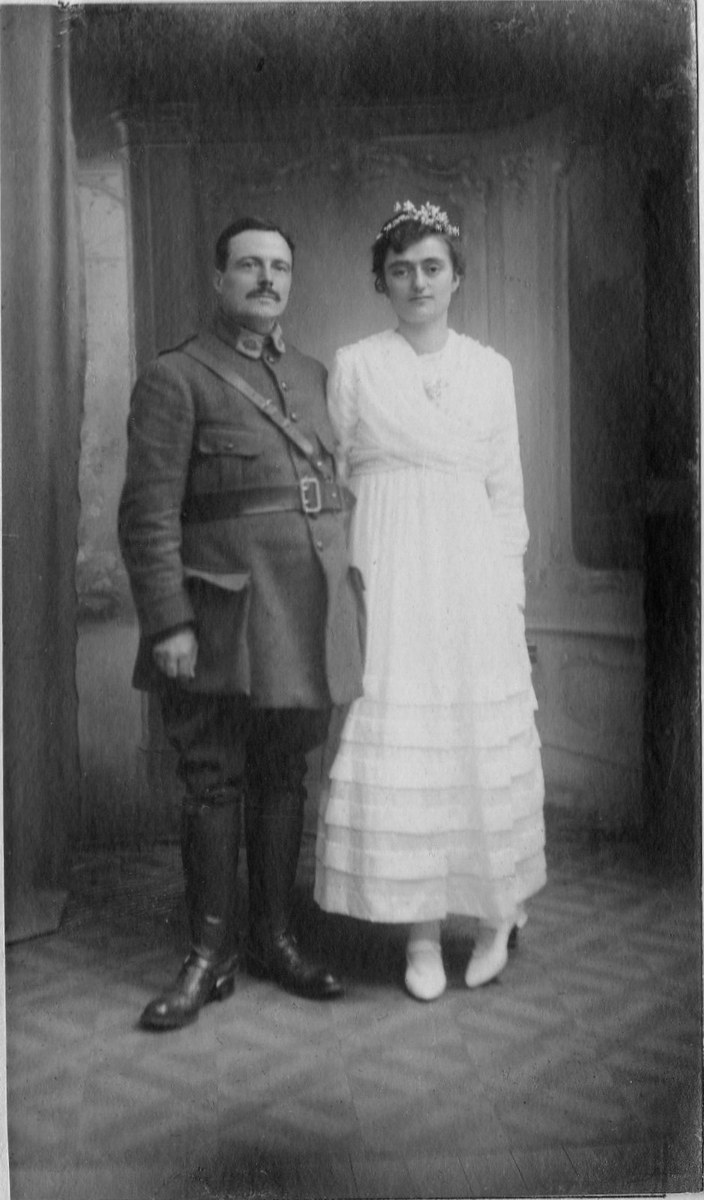
\includegraphics[width=0.94\linewidth,height=22mm,keepaspectratio]{illustrations/mariage_millau_1917.jpg}}
    \par\vspace{0.6mm}{\fontsize{5.8pt}{6.7pt}\selectfont Photographie officielle du mariage d'Hippolyte Combes (en uniforme d'interprète militaire) et de Marguerite Calmels à Millau (25 octobre 1917), entourés des familles Combes et Calmels.}
  \end{minipage}\hfill
  \begin{minipage}[b]{0.36\textwidth}
    \centering
    \setlength{\fboxsep}{0.7mm}\setlength{\fboxrule}{0.4pt}%
    \fcolorbox{gray!55}{white}{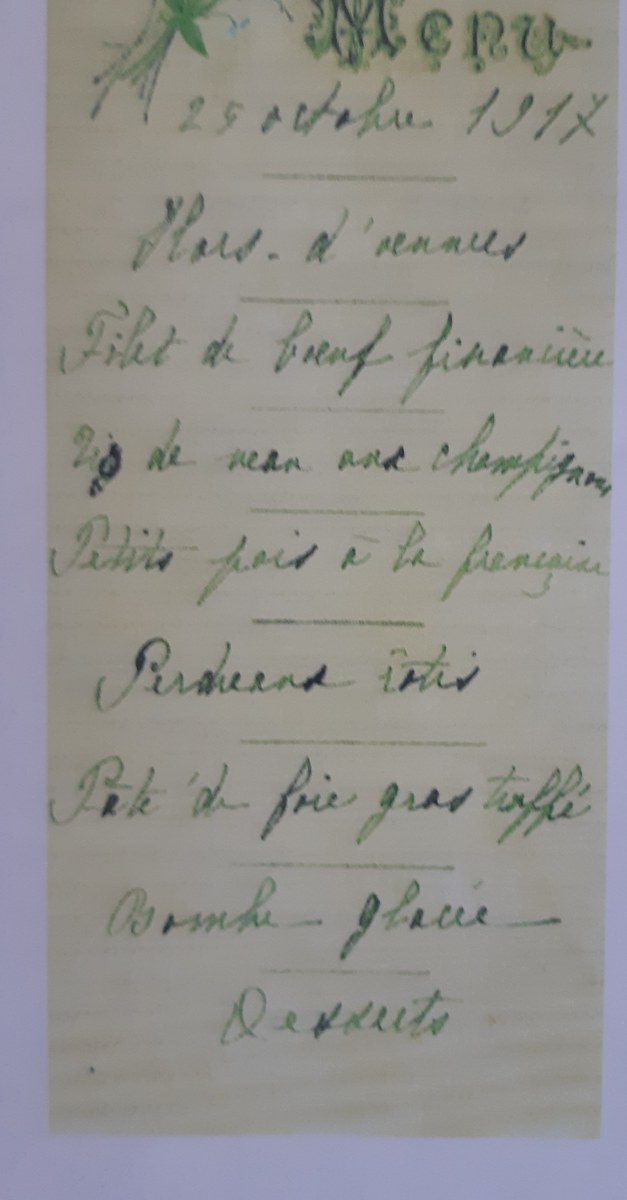
\includegraphics[width=0.94\linewidth,height=22mm,keepaspectratio]{illustrations/menu_mariage_1917.jpg}}
    \par\vspace{0.6mm}{\fontsize{5.8pt}{6.7pt}\selectfont Menu du repas de noces d'Hippolyte Combes et Marguerite Calmels au 10 rue Alfred-Guibert à Millau (25 octobre 1917). Archives familiales.}
  \end{minipage}
\end{center}
\clearpage

% =============================================================================
% VIS-A-VIS SPREAD : SCAN #128 (20251126_110048.jpg) — Vue 128
% =============================================================================
\cleardoubleevenpage
% --- En-tête du folio (Page paire / gauche : Transcription, apparat & double registre) ---
\noindent\rule{\textwidth}{0.5pt}\par\vspace{0.6mm}
\noindent\textbf{\footnotesize SCAN \#128 — VUE 128} \hfill {\scriptsize\texttt{20251126\_\allowbreak 110048.jpg}}\par\vspace{0.3mm}
\noindent{\fontsize{7.0pt}{8.2pt}\selectfont Départ en permission de la gare de Varennes et longue attente nocturne à Gézaincourt}\par\vspace{0.25mm}
\noindent{\fontsize{7.0pt}{8.2pt}\selectfont\textit{26 janvier 1917} \hfill \textit{Acheux, Gare de Varennes, Gézaincourt (Somme)}}\par\vspace{0.6mm}
\noindent\rule{\textwidth}{0.35pt}\par\vspace{1.0mm}
% --- Corps de la transcription diplomatique et apparat marginal en prolongement ---
{\renewcommand{\arraystretch}{0.89}%
\noindent\hspace*{3.5mm}\begin{tabular}{@{}p{100mm}@{\hspace{3.5mm}}p{55mm}@{}}
      \leavevmode\fontsize{7.0pt}{8.1pt}\selectfont\strut 26 Vendredi — \hfill{} Janvier /17\strut &  \\
      \leavevmode\fontsize{7.0pt}{8.1pt}\selectfont\strut Levé 8h 30 m.\strut &  \\
      \leavevmode\fontsize{7.0pt}{8.1pt}\selectfont\strut Nuit extt froide, gelé très fort. 1/2 jour, soleil\strut & \leavevmode\fontsize{6.3pt}{7.2pt}\selectfont\raggedright\arraybackslash\color{black!88}\textbf{3} \textbf{extt} \textit{extrêmement} ; \textbf{1/2 jour} milieu du jour, vers midi. \\
      \leavevmode\fontsize{7.0pt}{8.1pt}\selectfont\strut brillé et très vif éclat.\strut &  \\
      \leavevmode\llap{\fontsize{6.5pt}{7.5pt}\selectfont\color{darkgray}5\hspace{1.8mm}}\fontsize{7.0pt}{8.1pt}\selectfont\strut Matinée, achevé ranger mes affaires.\strut &  \\
      \leavevmode\fontsize{7.0pt}{8.1pt}\selectfont\strut A midi, fait prendre à gare 2 sacs par voiture\strut &  \\
      \leavevmode\fontsize{7.0pt}{8.1pt}\selectfont\strut qui fait service poste.\strut &  \\
      \leavevmode\fontsize{7.0pt}{8.1pt}\selectfont\strut Après déjeuner, venu à pied station, vers 2h.\strut &  \\
      \leavevmode\fontsize{7.0pt}{8.1pt}\selectfont\strut Attendu patiemment départ train — installé 2e cl. [addition interlinéaire : compartiment]\strut & \leavevmode\fontsize{6.3pt}{7.2pt}\selectfont\raggedright\arraybackslash\color{black!88}\textbf{9} \textbf{cl.} \textit{classe} ; \textbf{[addition interlinéaire : compartiment]} addition réellement visible ; rattachement à cette ligne proposé par la position. \\
      \leavevmode\llap{\fontsize{6.5pt}{7.5pt}\selectfont\color{darkgray}10\hspace{1.8mm}}\fontsize{7.0pt}{8.1pt}\selectfont\strut Soleil brûlant s/ les vitres, du côté de Varennes.\strut & \leavevmode\fontsize{6.3pt}{7.2pt}\selectfont\raggedright\arraybackslash\color{black!88}\textbf{10} \textbf{s/} \textit{sur}. \\
      \leavevmode\fontsize{7.0pt}{8.1pt}\selectfont\strut Champs tt couverts couche neige durcie\strut & \leavevmode\fontsize{6.3pt}{7.2pt}\selectfont\raggedright\arraybackslash\color{black!88}\textbf{11} \textbf{tt} \textit{tout}. \\
      \leavevmode\fontsize{7.0pt}{8.1pt}\selectfont\strut dont les particules, comme des grains de diamant,\strut &  \\
      \leavevmode\fontsize{7.0pt}{8.1pt}\selectfont\strut étincellent sous les rayons solaires.\strut &  \\
      \leavevmode\fontsize{7.0pt}{8.1pt}\selectfont\strut A la ligne de l'horizon, légère buée\strut &  \\
      \leavevmode\llap{\fontsize{6.5pt}{7.5pt}\selectfont\color{darkgray}15\hspace{1.8mm}}\fontsize{7.0pt}{8.1pt}\selectfont\strut blanchâtre, confondant terre \& ciel.\strut &  \\
      \leavevmode\fontsize{7.0pt}{8.1pt}\selectfont\strut 1 interprète, monté compartt. Entré en\strut & \leavevmode\fontsize{6.3pt}{7.2pt}\selectfont\raggedright\arraybackslash\color{black!88}\textbf{16} \textbf{compartt} \textit{compartiment}. \\
      \leavevmode\fontsize{7.0pt}{8.1pt}\selectfont\strut conversn \& échangé nos impressions \& jugements\strut & \leavevmode\fontsize{6.3pt}{7.2pt}\selectfont\raggedright\arraybackslash\color{black!88}\textbf{17} \textbf{conversn} \textit{conversation}. \\
      \leavevmode\fontsize{7.0pt}{8.1pt}\selectfont\strut sur les English.\strut & \leavevmode\fontsize{6.3pt}{7.2pt}\selectfont\raggedright\arraybackslash\color{black!88}\textbf{18} \textbf{English} \textit{angl.} Anglais. \\
      \leavevmode\fontsize{7.0pt}{8.1pt}\selectfont\strut Enfin, train démarré après 3h s.\strut &  \\
      \leavevmode\llap{\fontsize{6.5pt}{7.5pt}\selectfont\color{darkgray}20\hspace{1.8mm}}\fontsize{7.0pt}{8.1pt}\selectfont\strut A Gézaincourt, à 4h 30.\strut &  \\
      \leavevmode\fontsize{7.0pt}{8.1pt}\selectfont\strut Là, dû attendre correspce, ds salle surchauffée,\strut & \leavevmode\fontsize{6.3pt}{7.2pt}\selectfont\raggedright\arraybackslash\color{black!88}\textbf{21} \textbf{correspce} \textit{correspondance} ; \textbf{ds} \textit{dans}. \\
      \leavevmode\fontsize{7.0pt}{8.1pt}\selectfont\strut au 1/2 de voyrs, soldats permissionnaires ou paysans, foule\strut & \leavevmode\fontsize{6.3pt}{7.2pt}\selectfont\raggedright\arraybackslash\color{black!88}\textbf{22} \textbf{1/2} milieu, dans « au milieu de voyageurs » ; \textbf{voyrs} \textit{voyageurs}. \\
      \leavevmode\fontsize{7.0pt}{8.1pt}\selectfont\strut très bruyante. Train de Doullens, 3 h. de\strut &  \\
      \leavevmode\fontsize{7.0pt}{8.1pt}\selectfont\strut retard. Quitté Gézaincourt, à 10h 30 s.\strut &  \\
\end{tabular}}%
\par\vspace*{\fill}
% --- Deux registres de commentaires en bas de page (sans intitulés, distingués par filets et mise en page) ---
\noindent\rule{\textwidth}{0.5pt}\par\vspace{0.8mm}
{\fontsize{6.8pt}{8.0pt}\selectfont%
\noindent\normalfont Ligne 9 : compartiment est une addition interlinéaire, écrite sous la fin de installé 2e cl. et au-dessus de Varennes ; son rattachement syntaxique est proposé d’après la position. Ligne 16 : compartt abrège compartiment ; ligne 17, conversn conversation ; ligne 22, voyrs voyageurs. Le signe 1/2 signifie milieu dans 1/2 jour et au 1/2 de voyrs, selon des emplois temporel puis spatial. English est un nom anglais, désignant ici les Anglais.\par\vspace{0.75mm}
\noindent\rule{38mm}{0.4pt}\par\vspace{0.65mm}
\noindent\hspace*{5mm}\parbox{\dimexpr\textwidth-5mm\relax}{\fontsize{6.8pt}{8.0pt}\selectfont\color{black!82}\textbf{Départ et correspondance :} Le 26 janvier, deux sacs sont pris par la voiture du service postal, puis Combes gagne la station à pied. Varennes est un repère écrit à propos des vitres; le nom technique Acheux--Varennes et la voie métrique demandent une source ferroviaire. Arrivée à Gézaincourt 4 h 30, départ 10 h 30, avec trois heures de retard annoncées pour le train de Doullens. Le carnet décrit l’attente mais n’en attribue pas toutes les six heures au seul retard.}\par}
\newpage
% --- En-tête du fac-similé (Page impaire / droite : Scan original) ---
\noindent\rule{\textwidth}{0.5pt}\par\vspace{0.6mm}
\noindent\textbf{\fontsize{6.5pt}{7.6pt}\selectfont FAC-SIMILÉ EN VIS-À-VIS — VUE 128 (SCAN \#128)} \hfill {\fontsize{6.5pt}{7.6pt}\selectfont\texttt{20251126\_\allowbreak 110048.jpg}}\par\vspace{0.3mm}
\noindent{\fontsize{6.8pt}{8pt}\selectfont\textit{Livre-Journal d'Hippolyte Combes} — 26 janvier 1917 (Acheux, Gare de Varennes, Gézaincourt (Somme))}\par\vspace{0.6mm}
\noindent\rule{\textwidth}{0.35pt}\par\vspace*{\fill}
{\centering
  \setlength{\fboxsep}{1.2mm}%
  \setlength{\fboxrule}{0.4pt}%
  \fcolorbox{gray!55}{white}{%
    \includegraphics[width=0.94\textwidth,height=0.76\textheight,keepaspectratio]{\facsimiledir/20251126_110048.jpg}%
  }\par}
\vspace*{\fill}
\noindent\rule{\textwidth}{0.35pt}\par\vspace{0.5mm}
\noindent{\fontsize{6pt}{7.1pt}\selectfont\raggedright\color{darkgray}\textbf{Source :} Archives familiales Combes — Cliché numérique \texttt{20251126\_\allowbreak 110048.jpg} (Scan \#128/186, Vue 128). Haute définition : \texttt{scans\_haute\_qualite/\allowbreak 20251126\_\allowbreak 110048.jpg} ; version allégée : \texttt{scans\_compresses/\allowbreak 20251126\_\allowbreak 110048.jpg}.\par}
\newpage

% =============================================================================
% VIS-A-VIS SPREAD : SCAN #129 (20251126_110059.jpg) — Vue 129
% =============================================================================
\cleardoubleevenpage
% --- En-tête du folio (Page paire / gauche : Transcription, apparat & double registre) ---
\noindent\rule{\textwidth}{0.5pt}\par\vspace{0.6mm}
\noindent\textbf{\footnotesize SCAN \#129 — VUE 129} \hfill {\scriptsize\texttt{20251126\_\allowbreak 110059.jpg}}\par\vspace{0.3mm}
\noindent{\fontsize{7.0pt}{8.2pt}\selectfont Arrivée à Amiens à deux heures du matin et état de la caisse de voyage}\par\vspace{0.25mm}
\noindent{\fontsize{7.0pt}{8.2pt}\selectfont\textit{26 janvier 1917 (suite, nuit du 26 au 27)} \hfill \textit{Acheux, Gézaincourt, Amiens (Somme)}}\par\vspace{0.6mm}
\noindent\rule{\textwidth}{0.35pt}\par\vspace{1.0mm}
% --- Corps de la transcription diplomatique et apparat marginal en prolongement ---
{\renewcommand{\arraystretch}{1.02}%
\noindent\hspace*{3.5mm}\begin{tabular}{@{}p{100mm}@{\hspace{3.5mm}}p{55mm}@{}}
      \leavevmode\fontsize{7.8pt}{9.2pt}\selectfont\strut Ven. 26 (suite) \hfill{} Janvier 1917\strut & \leavevmode\fontsize{6.3pt}{7.2pt}\selectfont\raggedright\arraybackslash\color{black!88}\textbf{1} \textbf{Ven.} \textit{vendredi}. \\
      \leavevmode\fontsize{7.8pt}{9.2pt}\selectfont\strut Arrivé Amiens vers 2h m.\strut &  \\
      \leavevmode\fontsize{7.8pt}{9.2pt}\selectfont\strut Froid pénétrant — gelé très dur.\strut &  \\
      \leavevmode\fontsize{7.8pt}{9.2pt}\selectfont\strut Au ciel sombre, qq étoiles très brillantes.\strut & \leavevmode\fontsize{6.3pt}{7.2pt}\selectfont\raggedright\arraybackslash\color{black!88}\textbf{4} \textbf{qq} \textit{quelques}. \\
      \leavevmode\llap{\fontsize{6.5pt}{7.5pt}\selectfont\color{darkgray}5\hspace{1.8mm}}\fontsize{7.8pt}{9.2pt}\selectfont\strut [ — Voiturier, à Acheux : 1 f\strut & \leavevmode\fontsize{6.3pt}{7.2pt}\selectfont\raggedright\arraybackslash\color{black!88}\textbf{5} \textbf{[ — Voiturier} bloc comptable dans le corps de page, grand crochet gauche autographe. \\
      \leavevmode\fontsize{7.8pt}{9.2pt}\selectfont\strut (2 sacs à la gare)\strut &  \\
      \leavevmode\fontsize{7.8pt}{9.2pt}\selectfont\strut — A Gézaincourt : enregt bag. : 10 c\strut & \leavevmode\fontsize{6.3pt}{7.2pt}\selectfont\raggedright\arraybackslash\color{black!88}\textbf{7} \textbf{enregt} \textit{enregistrement} ; \textbf{bag.} \textit{bagages}. \\
      \leavevmode\fontsize{7.8pt}{9.2pt}\selectfont\strut (27 kg. — 2 sacs)\strut &  \\
      \leavevmode\fontsize{7.8pt}{9.2pt}\selectfont\strut En caisse, ce matin : 319 f 50 c ]\strut &  \\
\end{tabular}}%
\par\vspace*{\fill}
% --- Deux registres de commentaires en bas de page (sans intitulés, distingués par filets et mise en page) ---
\noindent\rule{\textwidth}{0.5pt}\par\vspace{0.8mm}
{\fontsize{6.8pt}{8.0pt}\selectfont%
\noindent\normalfont Ligne 1 : Ven. 26 (suite) reprend la date du départ ; l’arrivée vers deux heures du matin relatée à la ligne 2 appartient au voyage nocturne, également décrit à la vue 130. Lignes 5–9 : les dépenses et la somme en caisse sont réunies par un grand crochet gauche autographe dans le corps de page. Ligne 7 : enregt bag. se développe enregistrement des bagages. Le poids de 27 kg est inscrit dans une parenthèse, distinct du prix de l’enregistrement. La somme en caisse est un solde déclaré, sans que l’apparat l’assimile à toute une fortune ou à une origine déterminée.\par\vspace{0.75mm}
\noindent\rule{38mm}{0.4pt}\par\vspace{0.65mm}
\noindent\hspace*{5mm}\parbox{\dimexpr\textwidth-5mm\relax}{\fontsize{6.8pt}{8.0pt}\selectfont\color{black!82}\textbf{Nuit du 26 au 27 janvier :} L’arrivée à Amiens vers 2 h du matin reprend celle de 130, après le trajet et l’attente à Gézaincourt. L’encadré enregistre 1 f pour voiturier, 10 c pour enregistrement, 27 kg pour deux sacs, et l’encaisse 319 f 50. Les achats ultérieurs sont consignés ailleurs; cette somme n’a pas une affectation de fiançailles explicitement indiquée.}\par}
\newpage
% --- En-tête du fac-similé (Page impaire / droite : Scan original) ---
\noindent\rule{\textwidth}{0.5pt}\par\vspace{0.6mm}
\noindent\textbf{\fontsize{6.5pt}{7.6pt}\selectfont FAC-SIMILÉ EN VIS-À-VIS — VUE 129 (SCAN \#129)} \hfill {\fontsize{6.5pt}{7.6pt}\selectfont\texttt{20251126\_\allowbreak 110059.jpg}}\par\vspace{0.3mm}
\noindent{\fontsize{6.8pt}{8pt}\selectfont\textit{Livre-Journal d'Hippolyte Combes} — 26 janvier 1917 (suite, nuit du 26 au 27) (Acheux, Gézaincourt, Amiens (Somme))}\par\vspace{0.6mm}
\noindent\rule{\textwidth}{0.35pt}\par\vspace*{\fill}
{\centering
  \setlength{\fboxsep}{1.2mm}%
  \setlength{\fboxrule}{0.4pt}%
  \fcolorbox{gray!55}{white}{%
    \includegraphics[width=0.94\textwidth,height=0.76\textheight,keepaspectratio]{\facsimiledir/20251126_110059.jpg}%
  }\par}
\vspace*{\fill}
\noindent\rule{\textwidth}{0.35pt}\par\vspace{0.5mm}
\noindent{\fontsize{6pt}{7.1pt}\selectfont\raggedright\color{darkgray}\textbf{Source :} Archives familiales Combes — Cliché numérique \texttt{20251126\_\allowbreak 110059.jpg} (Scan \#129/186, Vue 129). Haute définition : \texttt{scans\_haute\_qualite/\allowbreak 20251126\_\allowbreak 110059.jpg} ; version allégée : \texttt{scans\_compresses/\allowbreak 20251126\_\allowbreak 110059.jpg}.\par}
\newpage

% =============================================================================
% VIS-A-VIS SPREAD : SCAN #130 (20251126_110124.jpg) — Vue 130
% =============================================================================
\cleardoubleevenpage
% --- En-tête du folio (Page paire / gauche : Transcription, apparat & double registre) ---
\noindent\rule{\textwidth}{0.5pt}\par\vspace{0.6mm}
\noindent\textbf{\footnotesize SCAN \#130 — VUE 130} \hfill {\scriptsize\texttt{20251126\_\allowbreak 110124.jpg}}\par\vspace{0.3mm}
\noindent{\fontsize{7.0pt}{8.2pt}\selectfont Nuit glaciale à la gare d'Amiens avec l'interprète Boilly et arrivée à Paris et Neuilly}\par\vspace{0.25mm}
\noindent{\fontsize{7.0pt}{8.2pt}\selectfont\textit{27 janvier 1917 (matin et midi)} \hfill \textit{Amiens, Paris (Gare du Nord, Gare d'Orsay), Neuilly-sur-Seine}}\par\vspace{0.6mm}
\noindent\rule{\textwidth}{0.35pt}\par\vspace{1.0mm}
% --- Corps de la transcription diplomatique et apparat marginal en prolongement ---
{\renewcommand{\arraystretch}{0.95}%
\noindent\hspace*{3.5mm}\begin{tabular}{@{}p{100mm}@{\hspace{3.5mm}}p{55mm}@{}}
      \leavevmode\fontsize{7.4pt}{8.6pt}\selectfont\strut Sam. 27 — \hfill{} Janv. 1917\strut & \leavevmode\fontsize{6.3pt}{7.2pt}\selectfont\raggedright\arraybackslash\color{black!88}\textbf{1} \textbf{Sam.} \textit{samedi} ; \textbf{Janv.} \textit{janvier}. \\
      \leavevmode\fontsize{7.4pt}{8.6pt}\selectfont\strut Train arrivé enfin à\strut &  \\
      \leavevmode\fontsize{7.4pt}{8.6pt}\selectfont\strut Amiens, vers 2h matin.\strut &  \\
      \leavevmode\fontsize{7.4pt}{8.6pt}\selectfont\strut En compagnie de 2 interprètes (dont l'1,\strut &  \\
      \leavevmode\llap{\fontsize{6.5pt}{7.5pt}\selectfont\color{darkgray}5\hspace{1.8mm}}\fontsize{7.4pt}{8.6pt}\selectfont\strut Boilly, est prof. à Pont-à-Mousson)\strut & \leavevmode\fontsize{6.3pt}{7.2pt}\selectfont\raggedright\arraybackslash\color{black!88}\textbf{5} \textbf{prof.} \textit{professeur}. \\
      \leavevmode\fontsize{7.4pt}{8.6pt}\selectfont\strut sorti gare, et allé à l'Abri du Soldat,\strut &  \\
      \leavevmode\fontsize{7.4pt}{8.6pt}\selectfont\strut Bvd Alsace-Lorraine. Aucune place.\strut & \leavevmode\fontsize{6.3pt}{7.2pt}\selectfont\raggedright\arraybackslash\color{black!88}\textbf{7} \textbf{Bvd} \textit{boulevard}. \\
      \leavevmode\fontsize{7.4pt}{8.6pt}\selectfont\strut Entré à la Y.M.C.A. Hut, à côté gare.\strut & \leavevmode\fontsize{6.3pt}{7.2pt}\selectfont\raggedright\arraybackslash\color{black!88}\textbf{8} \textbf{Y.M.C.A.} \textit{Young Men’s Christian Association, association chrétienne de jeunes gens} ; \textbf{Hut} \textit{angl.} baraque. \\
      \leavevmode\fontsize{7.4pt}{8.6pt}\selectfont\strut Puis durant des heures, déambulé\strut &  \\
      \leavevmode\llap{\fontsize{6.5pt}{7.5pt}\selectfont\color{darkgray}10\hspace{1.8mm}}\fontsize{7.4pt}{8.6pt}\selectfont\strut le long quai gare, en attendant train\strut &  \\
      \leavevmode\fontsize{7.4pt}{8.6pt}\selectfont\strut de Boulogne-Paris. Froid très vif.\strut &  \\
      \leavevmode\fontsize{7.4pt}{8.6pt}\selectfont\strut Enfin vers 5h 1/2 (2 h. de retard) train arrivé. Monté\strut &  \\
      \leavevmode\fontsize{7.4pt}{8.6pt}\selectfont\strut compartiment 2e cl., très confortable, mais\strut & \leavevmode\fontsize{6.3pt}{7.2pt}\selectfont\raggedright\arraybackslash\color{black!88}\textbf{13} \textbf{cl.} \textit{classe}. \\
      \leavevmode\fontsize{7.4pt}{8.6pt}\selectfont\strut y air brûlant, irrespirable.\strut &  \\
      \leavevmode\llap{\fontsize{6.5pt}{7.5pt}\selectfont\color{darkgray}15\hspace{1.8mm}}\fontsize{7.4pt}{8.6pt}\selectfont\strut Pu m'assoupir 1 peu.\strut &  \\
      \leavevmode\fontsize{7.4pt}{8.6pt}\selectfont\strut Paris, gare du Nord, vers 11h 15 m.\strut &  \\
      \leavevmode\fontsize{7.4pt}{8.6pt}\selectfont\strut Pris 1 fiacre et venu gare d'Orsay\strut &  \\
      \leavevmode\fontsize{7.4pt}{8.6pt}\selectfont\strut où billet et fait, en 10 minutes, enregistrer mes bagages.\strut &  \\
      \leavevmode\fontsize{7.4pt}{8.6pt}\selectfont\strut Me suis rendu par le métro à\strut &  \\
      \leavevmode\llap{\fontsize{6.5pt}{7.5pt}\selectfont\color{darkgray}20\hspace{1.8mm}}\fontsize{7.4pt}{8.6pt}\selectfont\strut Neuilly : Tuileries – Porte-Maillot.\strut &  \\
      \leavevmode\fontsize{7.4pt}{8.6pt}\selectfont\strut Après 5 m. de marche, arrivé\strut &  \\
      \leavevmode\fontsize{7.4pt}{8.6pt}\selectfont\strut rue d'Armenonville, no [?]6.\strut & \leavevmode\fontsize{6.3pt}{7.2pt}\selectfont\raggedright\arraybackslash\color{black!88}\textbf{22} \textbf{no} \textit{numéro} ; \textbf{[?]6} premier chiffre surchargé et non établi ; seule la finale 6 est assurée. \\
      \leavevmode\fontsize{7.4pt}{8.6pt}\selectfont\strut Maison luxueuse. Au 4e étage, à g.\strut & \leavevmode\fontsize{6.3pt}{7.2pt}\selectfont\raggedright\arraybackslash\color{black!88}\textbf{23} \textbf{g.} \textit{gauche}. \\
\end{tabular}}%
\par\vspace*{\fill}
% --- Deux registres de commentaires en bas de page (sans intitulés, distingués par filets et mise en page) ---
\noindent\rule{\textwidth}{0.5pt}\par\vspace{0.8mm}
{\fontsize{6.8pt}{8.0pt}\selectfont%
\noindent\normalfont Ligne 5 : prof. se développe professeur. Lignes 13 et 23 : cl. signifie classe et g. gauche, selon les syntagmes ferroviaire puis immobilier. Ligne 18 : billet désigne ici le billet de train et ne reçoit pas la traduction anglaise cantonnement, valable dans d’autres emplois du carnet. Ligne 22 : no abrège numéro ; la réserve porte sur le premier chiffre de [?]6, non sur le mot no. Seule la finale 6 est assurée.\par\vspace{0.75mm}
\noindent\rule{38mm}{0.4pt}\par\vspace{0.65mm}
\noindent\hspace*{5mm}\parbox{\dimexpr\textwidth-5mm\relax}{\fontsize{6.8pt}{8.0pt}\selectfont\color{black!82}\textbf{Amiens, Paris et Neuilly :} Attente à Amiens avec deux interprètes, dont Boilly, professeur à Pont-à-Mousson; recherche d’abri boulevard Alsace-Lorraine puis à la Y.M.C.A. Après Paris-Nord, gare d’Orsay et métro Tuileries--Porte-Maillot, Combes arrive rue d’Armenonville à Neuilly. La lettre du 26 novembre 1918 évoque la famille Faure et Germaine, mais ne fournit pas un parallèle de cette adresse. Le numéro [?]6 du carnet demeure réservé ; le renvoi de l’ancienne édition à la vue 051 ne le résout pas.}\par}
\newpage
% --- En-tête du fac-similé (Page impaire / droite : Scan original) ---
\noindent\rule{\textwidth}{0.5pt}\par\vspace{0.6mm}
\noindent\textbf{\fontsize{6.5pt}{7.6pt}\selectfont FAC-SIMILÉ EN VIS-À-VIS — VUE 130 (SCAN \#130)} \hfill {\fontsize{6.5pt}{7.6pt}\selectfont\texttt{20251126\_\allowbreak 110124.jpg}}\par\vspace{0.3mm}
\noindent{\fontsize{6.8pt}{8pt}\selectfont\textit{Livre-Journal d'Hippolyte Combes} — 27 janvier 1917 (matin et midi) (Amiens, Paris (Gare du Nord, Gare d'Orsay), Neuilly-sur-Seine)}\par\vspace{0.6mm}
\noindent\rule{\textwidth}{0.35pt}\par\vspace*{\fill}
{\centering
  \setlength{\fboxsep}{1.2mm}%
  \setlength{\fboxrule}{0.4pt}%
  \fcolorbox{gray!55}{white}{%
    \includegraphics[width=0.94\textwidth,height=0.76\textheight,keepaspectratio]{\facsimiledir/20251126_110124.jpg}%
  }\par}
\vspace*{\fill}
\noindent\rule{\textwidth}{0.35pt}\par\vspace{0.5mm}
\noindent{\fontsize{6pt}{7.1pt}\selectfont\raggedright\color{darkgray}\textbf{Source :} Archives familiales Combes — Cliché numérique \texttt{20251126\_\allowbreak 110124.jpg} (Scan \#130/186, Vue 130). Haute définition : \texttt{scans\_haute\_qualite/\allowbreak 20251126\_\allowbreak 110124.jpg} ; version allégée : \texttt{scans\_compresses/\allowbreak 20251126\_\allowbreak 110124.jpg}.\par}
\newpage

% =============================================================================
% VIS-A-VIS SPREAD : SCAN #131 (20251126_110135.jpg) — Vue 131
% =============================================================================
\cleardoubleevenpage
% --- En-tête du folio (Page paire / gauche : Transcription, apparat & double registre) ---
\noindent\rule{\textwidth}{0.5pt}\par\vspace{0.6mm}
\noindent\textbf{\footnotesize SCAN \#131 — VUE 131} \hfill {\scriptsize\texttt{20251126\_\allowbreak 110135.jpg}}\par\vspace{0.3mm}
\noindent{\fontsize{7.0pt}{8.2pt}\selectfont Déjeuner à Neuilly chez Mme Faure, visite chez l'opticien Imbert et départ pour Toulouse}\par\vspace{0.25mm}
\noindent{\fontsize{7.0pt}{8.2pt}\selectfont\textit{27 janvier 1917 (suite)} \hfill \textit{Neuilly-sur-Seine, Paris (Boulevard Saint-Michel, Hôtel de Ville, Gare d'Orsay)}}\par\vspace{0.6mm}
\noindent\rule{\textwidth}{0.35pt}\par\vspace{1.0mm}
% --- Corps de la transcription diplomatique et apparat marginal en prolongement ---
{\renewcommand{\arraystretch}{1.02}%
\noindent\hspace*{3.5mm}\begin{tabular}{@{}p{100mm}@{\hspace{3.5mm}}p{55mm}@{}}
      \leavevmode\fontsize{7.8pt}{9.2pt}\selectfont\strut Sam. 27 (suite) \hfill{} Janv. 1917\strut & \leavevmode\fontsize{6.3pt}{7.2pt}\selectfont\raggedright\arraybackslash\color{black!88}\textbf{1} \textbf{Sam.} \textit{samedi} ; \textbf{Janv.} \textit{janvier}. \\
      \leavevmode\fontsize{7.8pt}{9.2pt}\selectfont\strut au 4e ét., à g., appartt de Mme Faure.\strut & \leavevmode\fontsize{6.3pt}{7.2pt}\selectfont\raggedright\arraybackslash\color{black!88}\textbf{2} \textbf{ét.} \textit{étage} ; \textbf{g.} \textit{gauche} ; \textbf{appartt} \textit{appartement} ; \textbf{Mme} \textit{Madame}. \\
      \leavevmode\fontsize{7.8pt}{9.2pt}\selectfont\strut Y arrivé, vers midi 30 —\strut &  \\
      \leavevmode\fontsize{7.8pt}{9.2pt}\selectfont\strut Accueil très affectueux.\strut &  \\
      \leavevmode\llap{\fontsize{6.5pt}{7.5pt}\selectfont\color{darkgray}5\hspace{1.8mm}}\fontsize{7.8pt}{9.2pt}\selectfont\strut Déjeuné en famille. Mlle Germaine \& Marcel\strut & \leavevmode\fontsize{6.3pt}{7.2pt}\selectfont\raggedright\arraybackslash\color{black!88}\textbf{5} \textbf{Mlle} \textit{Mademoiselle}. \\
      \leavevmode\fontsize{7.8pt}{9.2pt}\selectfont\strut présents. Les 2 autres fils, Henri, aspirant, et André,\strut &  \\
      \leavevmode\fontsize{7.8pt}{9.2pt}\selectfont\strut préparant Polyte, absents.\strut & \leavevmode\fontsize{6.3pt}{7.2pt}\selectfont\raggedright\arraybackslash\color{black!88}\textbf{7} \textbf{Polyte} \textit{Polytechnique, dans « préparant Polytechnique »}. \\
      \leavevmode\fontsize{7.8pt}{9.2pt}\selectfont\strut Causé longuement, après repas.\strut &  \\
      \leavevmode\fontsize{7.8pt}{9.2pt}\selectfont\strut Vers 4h s., pris congé.\strut &  \\
      \leavevmode\llap{\fontsize{6.5pt}{7.5pt}\selectfont\color{darkgray}10\hspace{1.8mm}}\fontsize{7.8pt}{9.2pt}\selectfont\strut Par métro, venu sur Bvd St-Michel, ch. Imbert,\strut & \leavevmode\fontsize{6.3pt}{7.2pt}\selectfont\raggedright\arraybackslash\color{black!88}\textbf{10} \textbf{Bvd} \textit{boulevard} ; \textbf{St} \textit{Saint} ; \textbf{ch.} \textit{chez}. \\
      \leavevmode\fontsize{7.8pt}{9.2pt}\selectfont\strut mobilisé. Vu son remplaçant.\strut &  \\
      \leavevmode\fontsize{7.8pt}{9.2pt}\selectfont\strut Magasins de l'Hôtel de Ville, plusrs achats.\strut & \leavevmode\fontsize{6.3pt}{7.2pt}\selectfont\raggedright\arraybackslash\color{black!88}\textbf{12} \textbf{plusrs} \textit{plusieurs}. \\
      \leavevmode\fontsize{7.8pt}{9.2pt}\selectfont\strut Remonté rue de Rivoli. Dîné restaurant \&\strut &  \\
      \leavevmode\fontsize{7.8pt}{9.2pt}\selectfont\strut à 7h s., gare d'Orsay.\strut &  \\
      \leavevmode\llap{\fontsize{6.5pt}{7.5pt}\selectfont\color{darkgray}15\hspace{1.8mm}}\fontsize{7.8pt}{9.2pt}\selectfont\strut Descendu quais. Installé compartt bien\strut & \leavevmode\fontsize{6.3pt}{7.2pt}\selectfont\raggedright\arraybackslash\color{black!88}\textbf{15} \textbf{compartt} \textit{compartiment}. \\
      \leavevmode\fontsize{7.8pt}{9.2pt}\selectfont\strut chauffé.\strut &  \\
      \leavevmode\fontsize{7.8pt}{9.2pt}\selectfont\strut Départ train vers 7h 50 s. Qq soldats —\strut & \leavevmode\fontsize{6.3pt}{7.2pt}\selectfont\raggedright\arraybackslash\color{black!88}\textbf{17} \textbf{Qq} \textit{Quelques}. \\
      \leavevmode\fontsize{7.8pt}{9.2pt}\selectfont\strut Air très chaud.\strut &  \\
      \leavevmode\fontsize{7.8pt}{9.2pt}\selectfont\strut Peu à peu, me suis assoupi.\strut &  \\
\end{tabular}}%
\par\vspace*{\fill}
% --- Deux registres de commentaires en bas de page (sans intitulés, distingués par filets et mise en page) ---
\noindent\rule{\textwidth}{0.5pt}\par\vspace{0.8mm}
{\fontsize{6.8pt}{8.0pt}\selectfont%
\noindent\normalfont Ligne 2 : la reprise au 4e ét., à g. continue le syntagme final de la page précédente, sans qu’un texte manquant soit supposé. Ligne 7 : Polyte est une forme contractée de Polytechnique, dans une mention de préparation scolaire. Lignes 10–11 : Imbert est dit mobilisé et Combes voit son remplaçant ; la contraction ch. signifie chez. Les heures de départ ne reçoivent pas de notes répétitives.\par\vspace{0.75mm}
\noindent\rule{38mm}{0.4pt}\par\vspace{0.65mm}
\noindent\hspace*{5mm}\parbox{\dimexpr\textwidth-5mm\relax}{\fontsize{6.8pt}{8.0pt}\selectfont\color{black!82}\textbf{Famille Faure et achats :} Mme Faure reçoit Combes avec Germaine et Marcel; Henri est dit aspirant et André préparant Polyte. L’annexe familiale rapproche ce Marcel de l’époux de Solange Meynial et du futur Compagnon de la Libération. Le récit de captivité attribué aux lettres des 25–26 novembre 1918 dans l’ancienne édition est absent des pièces originales réexaminées. La notice officielle de l’Ordre donne une naissance le 30 janvier 1906 et un service en 1926–1927 ; elle interdit aussi d’attribuer cette captivité militaire au Compagnon. Le degré de parenté Calmels--Faure est lui-même discuté dans l’annexe. L’après-midi, remplaçant d’Imbert et achats aux Magasins de l’Hôtel de Ville.}\par}
\newpage
% --- En-tête du fac-similé (Page impaire / droite : Scan original) ---
\noindent\rule{\textwidth}{0.5pt}\par\vspace{0.6mm}
\noindent\textbf{\fontsize{6.5pt}{7.6pt}\selectfont FAC-SIMILÉ EN VIS-À-VIS — VUE 131 (SCAN \#131)} \hfill {\fontsize{6.5pt}{7.6pt}\selectfont\texttt{20251126\_\allowbreak 110135.jpg}}\par\vspace{0.3mm}
\noindent{\fontsize{6.8pt}{8pt}\selectfont\textit{Livre-Journal d'Hippolyte Combes} — 27 janvier 1917 (suite) (Neuilly-sur-Seine, Paris (Boulevard Saint-Michel, Hôtel de Ville, Gare d'Orsay))}\par\vspace{0.6mm}
\noindent\rule{\textwidth}{0.35pt}\par\vspace*{\fill}
{\centering
  \setlength{\fboxsep}{1.2mm}%
  \setlength{\fboxrule}{0.4pt}%
  \fcolorbox{gray!55}{white}{%
    \includegraphics[width=0.94\textwidth,height=0.76\textheight,keepaspectratio]{\facsimiledir/20251126_110135.jpg}%
  }\par}
\vspace*{\fill}
\noindent\rule{\textwidth}{0.35pt}\par\vspace{0.5mm}
\noindent{\fontsize{6pt}{7.1pt}\selectfont\raggedright\color{darkgray}\textbf{Source :} Archives familiales Combes — Cliché numérique \texttt{20251126\_\allowbreak 110135.jpg} (Scan \#131/186, Vue 131). Haute définition : \texttt{scans\_haute\_qualite/\allowbreak 20251126\_\allowbreak 110135.jpg} ; version allégée : \texttt{scans\_compresses/\allowbreak 20251126\_\allowbreak 110135.jpg}.\par}
\newpage

% =============================================================================
% VIS-A-VIS SPREAD : SCAN #132 (20251126_110149.jpg) — Vue 132
% =============================================================================
\cleardoubleevenpage
% --- En-tête du folio (Page paire / gauche : Transcription, apparat & double registre) ---
\noindent\rule{\textwidth}{0.5pt}\par\vspace{0.6mm}
\noindent\textbf{\footnotesize SCAN \#132 — VUE 132} \hfill {\scriptsize\texttt{20251126\_\allowbreak 110149.jpg}}\par\vspace{0.3mm}
\noindent{\fontsize{7.0pt}{8.2pt}\selectfont Dépenses parisiennes et arrivée matinale à Toulouse : souvenirs des disparus et visite de l'oncle Émile}\par\vspace{0.25mm}
\noindent{\fontsize{7.0pt}{8.2pt}\selectfont\textit{27 (comptes) – 28 janvier 1917 (matin)} \hfill \textit{Paris, Toulouse (Gare Matabiau, Saint-Michel, Sainte-Marie)}}\par\vspace{0.6mm}
\noindent\rule{\textwidth}{0.35pt}\par\vspace{1.0mm}
% --- Corps de la transcription diplomatique et apparat marginal en prolongement ---
{\renewcommand{\arraystretch}{0.95}%
\noindent\hspace*{3.5mm}\begin{tabular}{@{}p{100mm}@{\hspace{3.5mm}}p{55mm}@{}}
      \leavevmode\fontsize{7.4pt}{8.6pt}\selectfont\strut Sam. 27 \hfill{} Janv. /17\strut & \leavevmode\fontsize{6.3pt}{7.2pt}\selectfont\raggedright\arraybackslash\color{black!88}\textbf{1} \textbf{Sam.} \textit{samedi} ; \textbf{Janv.} \textit{janvier}. \\
      \leavevmode\fontsize{7.4pt}{8.6pt}\selectfont\strut Paris. Gare du Nord. Facteur : 20 c\strut &  \\
      \leavevmode\fontsize{7.4pt}{8.6pt}\selectfont\strut Gare d'Orsay : 10 c. | Cartes ples : 10 c\strut & \leavevmode\fontsize{6.3pt}{7.2pt}\selectfont\raggedright\arraybackslash\color{black!88}\textbf{3} \textbf{Cartes ples} \textit{cartes postales}. \\
      \leavevmode\fontsize{7.4pt}{8.6pt}\selectfont\strut Enregt 2 colis, 2 f 40 : 10 c\strut & \leavevmode\fontsize{6.3pt}{7.2pt}\selectfont\raggedright\arraybackslash\color{black!88}\textbf{4} \textbf{Enregt} \textit{Enregistrement}. \\
      \leavevmode\llap{\fontsize{6.5pt}{7.5pt}\selectfont\color{darkgray}5\hspace{1.8mm}}\fontsize{7.4pt}{8.6pt}\selectfont\strut Fiacre taximètre : 1 f 45 + 30 c = 1 f 75 c\strut &  \\
      \leavevmode\fontsize{7.4pt}{8.6pt}\selectfont\strut Métro : 15, 15 c | Dîner : 1 f 95 + 10 c\strut &  \\
      \leavevmode\fontsize{7.4pt}{8.6pt}\selectfont\strut Billet pour Toulouse : 11 f 15 c\strut &  \\
      \leavevmode\fontsize{7.4pt}{8.6pt}\selectfont\strut Magasins Hôtel de Ville : 1 brosse à cheveux : 3 f 95\strut &  \\
      \leavevmode\fontsize{7.4pt}{8.6pt}\selectfont\strut Brosse à souliers : 65 c. — Peigne fin : 1 f 25 c\strut &  \\
      \leavevmode\llap{\fontsize{6.5pt}{7.5pt}\selectfont\color{darkgray}10\hspace{1.8mm}}\fontsize{7.4pt}{8.6pt}\selectfont\strut Peigne ordre : 95 c. — Cirage noir : 50 c\strut & \leavevmode\fontsize{6.3pt}{7.2pt}\selectfont\raggedright\arraybackslash\color{black!88}\textbf{10} \textbf{ordre} \textit{ordinaire}. \\
      \leavevmode\fontsize{7.4pt}{8.6pt}\selectfont\strut Dimanche 28\strut &  \\
      \leavevmode\fontsize{7.4pt}{8.6pt}\selectfont\strut Voyage, terminé sans incidents.\strut &  \\
      \leavevmode\fontsize{7.4pt}{8.6pt}\selectfont\strut En approchant de Toulouse, souvenirs jeunesse\strut &  \\
      \leavevmode\fontsize{7.4pt}{8.6pt}\selectfont\strut revenus en foule esprit. Cru revoir mère et\strut &  \\
      \leavevmode\llap{\fontsize{6.5pt}{7.5pt}\selectfont\color{darkgray}15\hspace{1.8mm}}\fontsize{7.4pt}{8.6pt}\selectfont\strut sœurs, m'attendant, cme autrefois, gare.\strut & \leavevmode\fontsize{6.3pt}{7.2pt}\selectfont\raggedright\arraybackslash\color{black!88}\textbf{15} \textbf{cme} \textit{comme}. \\
      \leavevmode\fontsize{7.4pt}{8.6pt}\selectfont\strut Vers 8h 15, arrivée.\strut &  \\
      \leavevmode\fontsize{7.4pt}{8.6pt}\selectfont\strut Retiré 2 bagages. Pris tram St-Michel.\strut & \leavevmode\fontsize{6.3pt}{7.2pt}\selectfont\raggedright\arraybackslash\color{black!88}\textbf{17} \textbf{tram} \textit{tramway} ; \textbf{St} \textit{Saint}. \\
      \leavevmode\fontsize{7.4pt}{8.6pt}\selectfont\strut Matinée, ds mon appartt, à ranger\strut & \leavevmode\fontsize{6.3pt}{7.2pt}\selectfont\raggedright\arraybackslash\color{black!88}\textbf{18} \textbf{ds} \textit{dans} ; \textbf{appartt} \textit{appartement}. \\
      \leavevmode\fontsize{7.4pt}{8.6pt}\selectfont\strut affaires.\strut &  \\
      \leavevmode\llap{\fontsize{6.5pt}{7.5pt}\selectfont\color{darkgray}20\hspace{1.8mm}}\fontsize{7.4pt}{8.6pt}\selectfont\strut Oncle Émile, venu me surprendre à 10h 1/2.\strut &  \\
      \leavevmode\fontsize{7.4pt}{8.6pt}\selectfont\strut A midi, enfin, à Ste-Marie. Dû\strut & \leavevmode\fontsize{6.3pt}{7.2pt}\selectfont\raggedright\arraybackslash\color{black!88}\textbf{21} \textbf{Ste} \textit{Sainte}. \\
      \leavevmode\fontsize{7.4pt}{8.6pt}\selectfont\strut attendre tram 30 m. angle musée.\strut &  \\
\end{tabular}}%
\par\vspace*{\fill}
% --- Deux registres de commentaires en bas de page (sans intitulés, distingués par filets et mise en page) ---
\noindent\rule{\textwidth}{0.5pt}\par\vspace{0.8mm}
{\fontsize{6.8pt}{8.0pt}\selectfont%
\noindent\normalfont Lignes 2–10 : succession de dépenses dans le corps de page, sans crochet enveloppant ni disposition de marge latérale. Ligne 4 : Enregt signifie Enregistrement et le montant principal est distingué des 10 c qui suivent. Ligne 10 : ordre est une contraction d’ordinaire après Peigne, et non le substantif ordre. Lignes 13–15 : la mère et les sœurs sont évoquées par le diariste ; leurs noms et dates de décès n’appartiennent pas au texte de cette entrée et relèvent du commentaire historique.\par\vspace{0.75mm}
\noindent\rule{38mm}{0.4pt}\par\vspace{0.65mm}
\noindent\hspace*{5mm}\parbox{\dimexpr\textwidth-5mm\relax}{\fontsize{6.8pt}{8.0pt}\selectfont\color{black!82}\textbf{Retour à Toulouse :} Le 28 janvier, arrivée 8 h 15, souvenirs de mère et sœurs, rangement à l’appartement, visite d’oncle Émile à 10 h 30, puis Sainte-Marie. Le récit familial donne Anaïs Alric (1838--1907), Maria (1875--1903) et Joséphine (1873--1914), éclairant ce souvenir sans inscrire leurs noms dans le texte. L’identification d’Émile Crouzet (1842--1921, agent de change à Toulouse, témoin de 39 ans sur l’acte de naissance n° 139 de Marguerite Calmels en 1892) est étayée par l’état civil et Combes-annexe ; le seul prénom du carnet n’en est pas une preuve autonome.}\par}
\newpage
% --- En-tête du fac-similé (Page impaire / droite : Scan original) ---
\noindent\rule{\textwidth}{0.5pt}\par\vspace{0.6mm}
\noindent\textbf{\fontsize{6.5pt}{7.6pt}\selectfont FAC-SIMILÉ EN VIS-À-VIS — VUE 132 (SCAN \#132)} \hfill {\fontsize{6.5pt}{7.6pt}\selectfont\texttt{20251126\_\allowbreak 110149.jpg}}\par\vspace{0.3mm}
\noindent{\fontsize{6.8pt}{8pt}\selectfont\textit{Livre-Journal d'Hippolyte Combes} — 27 (comptes) – 28 janvier 1917 (matin) (Paris, Toulouse (Gare Matabiau, Saint-Michel, Sainte-Marie))}\par\vspace{0.6mm}
\noindent\rule{\textwidth}{0.35pt}\par\vspace*{\fill}
{\centering
  \setlength{\fboxsep}{1.2mm}%
  \setlength{\fboxrule}{0.4pt}%
  \fcolorbox{gray!55}{white}{%
    \includegraphics[width=0.94\textwidth,height=0.76\textheight,keepaspectratio]{\facsimiledir/20251126_110149.jpg}%
  }\par}
\vspace*{\fill}
\noindent\rule{\textwidth}{0.35pt}\par\vspace{0.5mm}
\noindent{\fontsize{6pt}{7.1pt}\selectfont\raggedright\color{darkgray}\textbf{Source :} Archives familiales Combes — Cliché numérique \texttt{20251126\_\allowbreak 110149.jpg} (Scan \#132/186, Vue 132). Haute définition : \texttt{scans\_haute\_qualite/\allowbreak 20251126\_\allowbreak 110149.jpg} ; version allégée : \texttt{scans\_compresses/\allowbreak 20251126\_\allowbreak 110149.jpg}.\par}
\newpage

% =============================================================================
% VIS-A-VIS SPREAD : SCAN #133 (20251126_110200.jpg) — Vue 133
% =============================================================================
\cleardoubleevenpage
% --- En-tête du folio (Page paire / gauche : Transcription, apparat & double registre) ---
\noindent\rule{\textwidth}{0.5pt}\par\vspace{0.6mm}
\noindent\textbf{\footnotesize SCAN \#133 — VUE 133} \hfill {\scriptsize\texttt{20251126\_\allowbreak 110200.jpg}}\par\vspace{0.3mm}
\noindent{\fontsize{7.0pt}{8.2pt}\selectfont Retrouvailles infiniment tendres avec Marguerite à Sainte-Marie (Toulouse)}\par\vspace{0.25mm}
\noindent{\fontsize{7.0pt}{8.2pt}\selectfont\textit{28 janvier 1917 (suite)} \hfill \textit{Toulouse (Quartier Sainte-Marie / Côte Pavée)}}\par\vspace{0.6mm}
\noindent\rule{\textwidth}{0.35pt}\par\vspace{1.0mm}
% --- Corps de la transcription diplomatique et apparat marginal en prolongement ---
{\renewcommand{\arraystretch}{1.02}%
\noindent\hspace*{3.5mm}\begin{tabular}{@{}p{100mm}@{\hspace{3.5mm}}p{55mm}@{}}
      \leavevmode\fontsize{7.8pt}{9.2pt}\selectfont\strut Dim. 28. (suite) — Janv. /17 —\strut & \leavevmode\fontsize{6.3pt}{7.2pt}\selectfont\raggedright\arraybackslash\color{black!88}\textbf{1} \textbf{Dim.} \textit{dimanche} ; \textbf{Janv.} \textit{janvier}. \\
      \leavevmode\fontsize{7.8pt}{9.2pt}\selectfont\strut Margte, sur la porte, m'attendait. Accueil\strut & \leavevmode\fontsize{6.3pt}{7.2pt}\selectfont\raggedright\arraybackslash\color{black!88}\textbf{2} \textbf{Margte} \textit{Marguerite}. \\
      \leavevmode\fontsize{7.8pt}{9.2pt}\selectfont\strut infiniment tendre. S'est montrée charmante.\strut &  \\
      \leavevmode\fontsize{7.8pt}{9.2pt}\selectfont\strut Vu Tante \& Madeleine.\strut &  \\
      \leavevmode\llap{\fontsize{6.5pt}{7.5pt}\selectfont\color{darkgray}5\hspace{1.8mm}}\fontsize{7.8pt}{9.2pt}\selectfont\strut Passé journée entière à Ste-Marie. Longues\strut & \leavevmode\fontsize{6.3pt}{7.2pt}\selectfont\raggedright\arraybackslash\color{black!88}\textbf{5} \textbf{Ste} \textit{Sainte}. \\
      \leavevmode\fontsize{7.8pt}{9.2pt}\selectfont\strut heures d'intime tête-à-tête av. Margte, dans\strut & \leavevmode\fontsize{6.3pt}{7.2pt}\selectfont\raggedright\arraybackslash\color{black!88}\textbf{6} \textbf{av.} \textit{avec} ; \textbf{Margte} \textit{Marguerite}. \\
      \leavevmode\fontsize{7.8pt}{9.2pt}\selectfont\strut le petit salon.\strut &  \\
      \leavevmode\fontsize{7.8pt}{9.2pt}\selectfont\strut Jean, monté à 6h 1/2 et dîné avec nous.\strut &  \\
      \leavevmode\fontsize{7.8pt}{9.2pt}\selectfont\strut Redescendu seul, à pied, à 9h s. Aucun tram.\strut & \leavevmode\fontsize{6.3pt}{7.2pt}\selectfont\raggedright\arraybackslash\color{black!88}\textbf{9} \textbf{tram} \textit{tramway}. \\
      \leavevmode\llap{\fontsize{6.5pt}{7.5pt}\selectfont\color{darkgray}10\hspace{1.8mm}}\fontsize{7.8pt}{9.2pt}\selectfont\strut Margte, vraiment exquise de simplicité \& de charme,\strut & \leavevmode\fontsize{6.3pt}{7.2pt}\selectfont\raggedright\arraybackslash\color{black!88}\textbf{10} \textbf{Margte} \textit{Marguerite}. \\
      \leavevmode\fontsize{7.8pt}{9.2pt}\selectfont\strut vive, spontanée, aimante, affectueuse au possible.\strut &  \\
      \leavevmode\fontsize{7.8pt}{9.2pt}\selectfont\strut Mes sentiments à son égard, douceur infinie.\strut &  \\
      \leavevmode\fontsize{7.8pt}{9.2pt}\selectfont\strut Causeries délicieuses sur les sujets les plus\strut &  \\
      \leavevmode\fontsize{7.8pt}{9.2pt}\selectfont\strut divers.\strut &  \\
      \leavevmode\llap{\fontsize{6.5pt}{7.5pt}\selectfont\color{darkgray}15\hspace{1.8mm}}\fontsize{7.8pt}{9.2pt}\selectfont\strut [ — Trams : 10 c, 10 c — ]\strut & \leavevmode\fontsize{6.3pt}{7.2pt}\selectfont\raggedright\arraybackslash\color{black!88}\textbf{15} \textbf{[ — Trams} compte au bas de page, tiret autographe ; crochets éditoriaux ; \textbf{Trams} \textit{Tramways}. \\
\end{tabular}}%
\par\vspace*{\fill}
% --- Deux registres de commentaires en bas de page (sans intitulés, distingués par filets et mise en page) ---
\noindent\rule{\textwidth}{0.5pt}\par\vspace{0.8mm}
{\fontsize{6.8pt}{8.0pt}\selectfont%
\noindent\normalfont Lignes 2, 6 et 10 : Margte est la contraction du prénom Marguerite ; les trois occurrences sont expliquées à leur place. Ligne 6 : av. signifie avec, omission de l’ancien apparat. Ligne 15 : deux dépenses de tramways écrites au bas de la page et précédées d’un tiret, sans crochet autographe visible. Les appréciations affectives du récit ne prouvent pas la disparition définitive des inquiétudes consignées auparavant.\par\vspace{0.75mm}
\noindent\rule{38mm}{0.4pt}\par\vspace{0.65mm}
\noindent\hspace*{5mm}\parbox{\dimexpr\textwidth-5mm\relax}{\fontsize{6.8pt}{8.0pt}\selectfont\color{black!82}\textbf{Sainte-Marie :} Accueil tendre de Margte, visite de Tante et Madeleine, puis arrivée de Jean à 6 h 30. Le rapprochement de Tante avec Élisabeth Calmels, épouse d’Émile Crouzet, et de Jean avec l’abbé Jean Crouzet vient du récit familial (Combes-annexe), non de leurs seuls noms dans cette page. Madeleine Calmels est déjà mariée au docteur Fernand Vincens depuis juillet 1907 (Combes-3-part 1). L’effacement définitif des appréhensions de Noël n’est pas établi par la tendresse de cette journée.}\par}
\newpage
% --- En-tête du fac-similé (Page impaire / droite : Scan original) ---
\noindent\rule{\textwidth}{0.5pt}\par\vspace{0.6mm}
\noindent\textbf{\fontsize{6.5pt}{7.6pt}\selectfont FAC-SIMILÉ EN VIS-À-VIS — VUE 133 (SCAN \#133)} \hfill {\fontsize{6.5pt}{7.6pt}\selectfont\texttt{20251126\_\allowbreak 110200.jpg}}\par\vspace{0.3mm}
\noindent{\fontsize{6.8pt}{8pt}\selectfont\textit{Livre-Journal d'Hippolyte Combes} — 28 janvier 1917 (suite) (Toulouse (Quartier Sainte-Marie / Côte Pavée))}\par\vspace{0.6mm}
\noindent\rule{\textwidth}{0.35pt}\par\vspace*{\fill}
{\centering
  \setlength{\fboxsep}{1.2mm}%
  \setlength{\fboxrule}{0.4pt}%
  \fcolorbox{gray!55}{white}{%
    \includegraphics[width=0.94\textwidth,height=0.76\textheight,keepaspectratio]{\facsimiledir/20251126_110200.jpg}%
  }\par}
\vspace*{\fill}
\noindent\rule{\textwidth}{0.35pt}\par\vspace{0.5mm}
\noindent{\fontsize{6pt}{7.1pt}\selectfont\raggedright\color{darkgray}\textbf{Source :} Archives familiales Combes — Cliché numérique \texttt{20251126\_\allowbreak 110200.jpg} (Scan \#133/186, Vue 133). Haute définition : \texttt{scans\_haute\_qualite/\allowbreak 20251126\_\allowbreak 110200.jpg} ; version allégée : \texttt{scans\_compresses/\allowbreak 20251126\_\allowbreak 110200.jpg}.\par}
\newpage

% =============================================================================
% VIS-A-VIS SPREAD : SCAN #134 (20251126_110216.jpg) — Vue 134
% =============================================================================
\cleardoubleevenpage
% --- En-tête du folio (Page paire / gauche : Transcription, apparat & double registre) ---
\noindent\rule{\textwidth}{0.5pt}\par\vspace{0.6mm}
\noindent\textbf{\footnotesize SCAN \#134 — VUE 134} \hfill {\scriptsize\texttt{20251126\_\allowbreak 110216.jpg}}\par\vspace{0.3mm}
\noindent{\fontsize{7.0pt}{8.2pt}\selectfont Le panier de fleurs de Nice et le pèlerinage de jeunesse aux cryptes de Saint-Sernin}\par\vspace{0.25mm}
\noindent{\fontsize{7.0pt}{8.2pt}\selectfont\textit{29 janvier 1917} \hfill \textit{Toulouse (Gare Matabiau, Sainte-Marie, Basilique Saint-Sernin, Place du Capitole, Rue d'Alsace, Côte Pavée)}}\par\vspace{0.6mm}
\noindent\rule{\textwidth}{0.35pt}\par\vspace{1.0mm}
% --- Corps de la transcription diplomatique et apparat marginal en prolongement ---
{\renewcommand{\arraystretch}{0.89}%
\noindent\hspace*{3.5mm}\begin{tabular}{@{}p{100mm}@{\hspace{3.5mm}}p{55mm}@{}}
      \leavevmode\fontsize{7.0pt}{8.1pt}\selectfont\strut Lundi 29. \hfill{} — Janvier 1917 —\strut &  \\
      \leavevmode\fontsize{7.0pt}{8.1pt}\selectfont\strut Levé 7h 1/2.\strut &  \\
      \leavevmode\fontsize{7.0pt}{8.1pt}\selectfont\strut Matin, temps 1 peu froid. Journée, soleil pâle.\strut &  \\
      \leavevmode\fontsize{7.0pt}{8.1pt}\selectfont\strut Allumé gd feu cheminée chambre rue. Goûté\strut & \leavevmode\fontsize{6.3pt}{7.2pt}\selectfont\raggedright\arraybackslash\color{black!88}\textbf{4} \textbf{gd} \textit{grand}. \\
      \leavevmode\llap{\fontsize{6.5pt}{7.5pt}\selectfont\color{darkgray}5\hspace{1.8mm}}\fontsize{7.0pt}{8.1pt}\selectfont\strut confort chambre retrouvée.\strut &  \\
      \leavevmode\fontsize{7.0pt}{8.1pt}\selectfont\strut Venu gare. Me suis fait livrer, non\strut &  \\
      \leavevmode\fontsize{7.0pt}{8.1pt}\selectfont\strut sans peine, panier fleurs Nice. Colis sans\strut &  \\
      \leavevmode\fontsize{7.0pt}{8.1pt}\selectfont\strut étiquette, ouverture et feuille postale disparues.\strut &  \\
      \leavevmode\fontsize{7.0pt}{8.1pt}\selectfont\strut Vers midi, enfin, de nouveau à Ste-Marie.\strut & \leavevmode\fontsize{6.3pt}{7.2pt}\selectfont\raggedright\arraybackslash\color{black!88}\textbf{9} \textbf{Ste} \textit{Sainte}. \\
      \leavevmode\llap{\fontsize{6.5pt}{7.5pt}\selectfont\color{darkgray}10\hspace{1.8mm}}\fontsize{7.0pt}{8.1pt}\selectfont\strut Après déjeuner, Marg. \& Madne, descendues\strut & \leavevmode\fontsize{6.3pt}{7.2pt}\selectfont\raggedright\arraybackslash\color{black!88}\textbf{10} \textbf{Marg.} \textit{Marguerite} ; \textbf{Madne} \textit{Madeleine}. \\
      \leavevmode\fontsize{7.0pt}{8.1pt}\selectfont\strut en ville avec moi.\strut &  \\
      \leavevmode\fontsize{7.0pt}{8.1pt}\selectfont\strut Visité longuement basilique St-Sernin\strut & \leavevmode\fontsize{6.3pt}{7.2pt}\selectfont\raggedright\arraybackslash\color{black!88}\textbf{12} \textbf{St} \textit{Saint}. \\
      \leavevmode\fontsize{7.0pt}{8.1pt}\selectfont\strut et surtout les cryptes. Toute ma jeunesse\strut &  \\
      \leavevmode\fontsize{7.0pt}{8.1pt}\selectfont\strut réveillée, dans \& autour de cette admirable\strut &  \\
      \leavevmode\llap{\fontsize{6.5pt}{7.5pt}\selectfont\color{darkgray}15\hspace{1.8mm}}\fontsize{7.0pt}{8.1pt}\selectfont\strut église romane.\strut &  \\
      \leavevmode\fontsize{7.0pt}{8.1pt}\selectfont\strut Magasins du Capitole \& Labit.\strut &  \\
      \leavevmode\fontsize{7.0pt}{8.1pt}\selectfont\strut Remonté 1 peu Rue Alsace.\strut &  \\
      \leavevmode\fontsize{7.0pt}{8.1pt}\selectfont\strut Enfin, allé prendre au Capitole\strut &  \\
      \leavevmode\fontsize{7.0pt}{8.1pt}\selectfont\strut notre tram p. Côte Pavée.\strut & \leavevmode\fontsize{6.3pt}{7.2pt}\selectfont\raggedright\arraybackslash\color{black!88}\textbf{19} \textbf{tram} \textit{tramway} ; \textbf{p.} \textit{pour}. \\
      \leavevmode\llap{\fontsize{6.5pt}{7.5pt}\selectfont\color{darkgray}20\hspace{1.8mm}}\fontsize{7.0pt}{8.1pt}\selectfont\strut A 9h s., quitté, hélas! Ste-Marie.\strut & \leavevmode\fontsize{6.3pt}{7.2pt}\selectfont\raggedright\arraybackslash\color{black!88}\textbf{20} \textbf{Ste} \textit{Sainte}. \\
      \leavevmode\fontsize{7.0pt}{8.1pt}\selectfont\strut [ — Trams : 10, 10, 10 c, 60, 10 c —\strut & \leavevmode\fontsize{6.3pt}{7.2pt}\selectfont\raggedright\arraybackslash\color{black!88}\textbf{21} \textbf{[ — Trams} bloc de dépenses, crochet gauche autographe ; \textbf{Trams} \textit{Tramways}. \\
      \leavevmode\fontsize{7.0pt}{8.1pt}\selectfont\strut Mag. du Capitole : boîte de 3 savonnettes : 2 f 90\strut & \leavevmode\fontsize{6.3pt}{7.2pt}\selectfont\raggedright\arraybackslash\color{black!88}\textbf{22} \textbf{Mag.} \textit{Magasins}. \\
      \leavevmode\fontsize{7.0pt}{8.1pt}\selectfont\strut Brosse à dents p. Margte : 2 f 25 c — Ctes ples : 30 c\strut & \leavevmode\fontsize{6.3pt}{7.2pt}\selectfont\raggedright\arraybackslash\color{black!88}\textbf{23} \textbf{p.} \textit{pour} ; \textbf{Margte} \textit{Marguerite} ; \textbf{Ctes ples} \textit{cartes postales}. \\
      \leavevmode\fontsize{7.0pt}{8.1pt}\selectfont\strut Cartes pour visiter cryptes de St-Sernin : 1 f — ]\strut & \leavevmode\fontsize{6.3pt}{7.2pt}\selectfont\raggedright\arraybackslash\color{black!88}\textbf{24} \textbf{St} \textit{Saint}. \\
\end{tabular}}%
\par\vspace*{\fill}
% --- Deux registres de commentaires en bas de page (sans intitulés, distingués par filets et mise en page) ---
\noindent\rule{\textwidth}{0.5pt}\par\vspace{0.8mm}
{\fontsize{6.8pt}{8.0pt}\selectfont%
\noindent\normalfont Ligne 10 : Marg. et Madne sont les prénoms contractés Marguerite et Madeleine. Lignes 19 et 23 : p. signifie pour, avec deux destinataires différents, la Côte Pavée puis Marguerite. Ligne 22 : Mag. abrège Magasins. Lignes 21–24 : bloc de dépenses introduit par un crochet gauche autographe. La jeunesse évoquée devant Saint-Sernin est un élément du récit ; les adresses de domicile familial n’y sont pas écrites et relèvent de la notice historique.\par\vspace{0.75mm}
\noindent\rule{38mm}{0.4pt}\par\vspace{0.65mm}
\noindent\hspace*{5mm}\parbox{\dimexpr\textwidth-5mm\relax}{\fontsize{6.8pt}{8.0pt}\selectfont\color{black!82}\textbf{Fleurs, Saint-Sernin et Labit :} Le 29 janvier, panier de fleurs venu de Nice, puis visite de Saint-Sernin et des cryptes avec Marg. et Madne. Le télégramme à Spagnol de 136 et le mandat de 158 peuvent être rapprochés du panier, sans établir que chaque envoi concernait un même colis. Les Magasins du Capitole et Labit sont nommés. La notice INHA AGORHA 321 sur Georges Labit donne Antoine Labit, fondateur de la Maison Universelle, pour son père; l’identification de l’enseigne ne modifie pas la désignation manuscrite.}\par}
\newpage
% --- En-tête du fac-similé (Page impaire / droite : Scan original) ---
\noindent\rule{\textwidth}{0.5pt}\par\vspace{0.6mm}
\noindent\textbf{\fontsize{6.5pt}{7.6pt}\selectfont FAC-SIMILÉ EN VIS-À-VIS — VUE 134 (SCAN \#134)} \hfill {\fontsize{6.5pt}{7.6pt}\selectfont\texttt{20251126\_\allowbreak 110216.jpg}}\par\vspace{0.3mm}
\noindent{\fontsize{6.8pt}{8pt}\selectfont\textit{Livre-Journal d'Hippolyte Combes} — 29 janvier 1917 (Toulouse (Gare Matabiau, Sainte-Marie, Basilique Saint-Sernin, Place du Capitole, Rue d'Alsace, Côte Pavée))}\par\vspace{0.6mm}
\noindent\rule{\textwidth}{0.35pt}\par\vspace*{\fill}
{\centering
  \setlength{\fboxsep}{1.2mm}%
  \setlength{\fboxrule}{0.4pt}%
  \fcolorbox{gray!55}{white}{%
    \includegraphics[width=0.94\textwidth,height=0.76\textheight,keepaspectratio]{\facsimiledir/20251126_110216.jpg}%
  }\par}
\vspace*{\fill}
\noindent\rule{\textwidth}{0.35pt}\par\vspace{0.5mm}
\noindent{\fontsize{6pt}{7.1pt}\selectfont\raggedright\color{darkgray}\textbf{Source :} Archives familiales Combes — Cliché numérique \texttt{20251126\_\allowbreak 110216.jpg} (Scan \#134/186, Vue 134). Haute définition : \texttt{scans\_haute\_qualite/\allowbreak 20251126\_\allowbreak 110216.jpg} ; version allégée : \texttt{scans\_compresses/\allowbreak 20251126\_\allowbreak 110216.jpg}.\par}
\newpage

% =============================================================================
% VIS-A-VIS SPREAD : SCAN #135 (20251126_110233.jpg) — Vue 135
% =============================================================================
\cleardoubleevenpage
% --- En-tête du folio (Page paire / gauche : Transcription, apparat & double registre) ---
\noindent\rule{\textwidth}{0.5pt}\par\vspace{0.6mm}
\noindent\textbf{\footnotesize SCAN \#135 — VUE 135} \hfill {\scriptsize\texttt{20251126\_\allowbreak 110233.jpg}}\par\vspace{0.3mm}
\noindent{\fontsize{7.0pt}{8.2pt}\selectfont Visite à Mme de Labarthe et conférence d'Ernest Zyromski sur Maurice de Guérin}\par\vspace{0.25mm}
\noindent{\fontsize{7.0pt}{8.2pt}\selectfont\textit{30 janvier 1917} \hfill \textit{Toulouse, Sainte-Marie ; lieu de la conférence non précisé}}\par\vspace{0.6mm}
\noindent\rule{\textwidth}{0.35pt}\par\vspace{1.0mm}
% --- Corps de la transcription diplomatique et apparat marginal en prolongement ---
{\renewcommand{\arraystretch}{0.95}%
\noindent\hspace*{3.5mm}\begin{tabular}{@{}p{100mm}@{\hspace{3.5mm}}p{55mm}@{}}
      \leavevmode\fontsize{7.4pt}{8.6pt}\selectfont\strut Mardi 30. \hfill{} Janvier 1917 —\strut &  \\
      \leavevmode\fontsize{7.4pt}{8.6pt}\selectfont\strut Levé 7h m. Allumé gd feu\strut & \leavevmode\fontsize{6.3pt}{7.2pt}\selectfont\raggedright\arraybackslash\color{black!88}\textbf{2} \textbf{gd} \textit{grand}. \\
      \leavevmode\fontsize{7.4pt}{8.6pt}\selectfont\strut chambre. Me suis prélassé s/ fauteuil. Joui\strut & \leavevmode\fontsize{6.3pt}{7.2pt}\selectfont\raggedright\arraybackslash\color{black!88}\textbf{3} \textbf{s/} \textit{sur}. \\
      \leavevmode\fontsize{7.4pt}{8.6pt}\selectfont\strut de mon bien-être \& repos de l'heure présente.\strut &  \\
      \leavevmode\llap{\fontsize{6.5pt}{7.5pt}\selectfont\color{darkgray}5\hspace{1.8mm}}\fontsize{7.4pt}{8.6pt}\selectfont\strut Évoqué passé sans mélancolie.\strut &  \\
      \leavevmode\fontsize{7.4pt}{8.6pt}\selectfont\strut Matin, visite à Mme de Labarthe. L'ai\strut & \leavevmode\fontsize{6.3pt}{7.2pt}\selectfont\raggedright\arraybackslash\color{black!88}\textbf{6} \textbf{Mme} \textit{Madame}. \\
      \leavevmode\fontsize{7.4pt}{8.6pt}\selectfont\strut revue av. un plaisir extrême.\strut & \leavevmode\fontsize{6.3pt}{7.2pt}\selectfont\raggedright\arraybackslash\color{black!88}\textbf{7} \textbf{av.} \textit{avec}. \\
      \leavevmode\fontsize{7.4pt}{8.6pt}\selectfont\strut Monté, cme d'habitude, à Ste-Marie pour\strut & \leavevmode\fontsize{6.3pt}{7.2pt}\selectfont\raggedright\arraybackslash\color{black!88}\textbf{8} \textbf{cme} \textit{comme} ; \textbf{Ste} \textit{Sainte}. \\
      \leavevmode\fontsize{7.4pt}{8.6pt}\selectfont\strut déjeuner.\strut &  \\
      \leavevmode\llap{\fontsize{6.5pt}{7.5pt}\selectfont\color{darkgray}10\hspace{1.8mm}}\fontsize{7.4pt}{8.6pt}\selectfont\strut Après-midi, assisté conférce de M. Zyromski\strut & \leavevmode\fontsize{6.3pt}{7.2pt}\selectfont\raggedright\arraybackslash\color{black!88}\textbf{10} \textbf{conférce} \textit{conférence} ; \textbf{M.} \textit{Monsieur}. \\
      \leavevmode\fontsize{7.4pt}{8.6pt}\selectfont\strut sur Maurice de Guérin (Influence de la Bretagne\strut &  \\
      \leavevmode\fontsize{7.4pt}{8.6pt}\selectfont\strut \& de Lamennais). Admirablt écrite. Passages\strut & \leavevmode\fontsize{6.3pt}{7.2pt}\selectfont\raggedright\arraybackslash\color{black!88}\textbf{12} \textbf{Admirablt} \textit{Admirablement}. \\
      \leavevmode\fontsize{7.4pt}{8.6pt}\selectfont\strut remarquables fond et forme. Vrai\strut &  \\
      \leavevmode\fontsize{7.4pt}{8.6pt}\selectfont\strut régal littéraire.\strut &  \\
      \leavevmode\llap{\fontsize{6.5pt}{7.5pt}\selectfont\color{darkgray}15\hspace{1.8mm}}\fontsize{7.4pt}{8.6pt}\selectfont\strut Fini journée en cie de Margte —\strut & \leavevmode\fontsize{6.3pt}{7.2pt}\selectfont\raggedright\arraybackslash\color{black!88}\textbf{15} \textbf{cie} \textit{compagnie, dans « en compagnie de Marguerite »} ; \textbf{Margte} \textit{Marguerite}. \\
      \leavevmode\fontsize{7.4pt}{8.6pt}\selectfont\strut [ — Cartes ples : 10 c.\strut & \leavevmode\fontsize{6.3pt}{7.2pt}\selectfont\raggedright\arraybackslash\color{black!88}\textbf{16} \textbf{[ — Cartes ples} bloc comptable, grand crochet gauche autographe ; \textbf{Cartes ples} \textit{cartes postales}. \\
      \leavevmode\fontsize{7.4pt}{8.6pt}\selectfont\strut — 1 ramette papier vélin : 1 f 25\strut &  \\
      \leavevmode\fontsize{7.4pt}{8.6pt}\selectfont\strut (moyen format)\strut & \leavevmode\fontsize{6.3pt}{7.2pt}\selectfont\raggedright\arraybackslash\color{black!88}\textbf{18} \textbf{(moyen format)} précision sur le papier, reportée sous le poste précédent. \\
      \leavevmode\fontsize{7.4pt}{8.6pt}\selectfont\strut 2 paquets d'enveloppes : 80 c.\strut &  \\
      \leavevmode\llap{\fontsize{6.5pt}{7.5pt}\selectfont\color{darkgray}20\hspace{1.8mm}}\fontsize{7.4pt}{8.6pt}\selectfont\strut Trams : 10 c, 60 c, 10 c.\strut & \leavevmode\fontsize{6.3pt}{7.2pt}\selectfont\raggedright\arraybackslash\color{black!88}\textbf{20} \textbf{Trams} \textit{Tramways}. \\
      \leavevmode\fontsize{7.4pt}{8.6pt}\selectfont\strut Le Miroir des Modes (no de janvier) : 1 f — ]\strut & \leavevmode\fontsize{6.3pt}{7.2pt}\selectfont\raggedright\arraybackslash\color{black!88}\textbf{21} \textbf{no} \textit{numéro}. \\
\end{tabular}}%
\par\vspace*{\fill}
% --- Deux registres de commentaires en bas de page (sans intitulés, distingués par filets et mise en page) ---
\noindent\rule{\textwidth}{0.5pt}\par\vspace{0.8mm}
{\fontsize{6.8pt}{8.0pt}\selectfont%
\noindent\normalfont Lignes 10–12 : conférce se développe conférence et Admirablt admirablement ; les appréciations portent sur la conférence, dont le lieu précis n’est pas donné. Ligne 15 : cie signifie compagnie dans « en compagnie de Marguerite », et non compagnie militaire. Ligne 21 : no est numéro, à propos du Miroir des Modes. Le compte des lignes 16–21 est introduit par un grand crochet autographe à gauche ; moyen format est une précision entre parenthèses reportée sous l’achat de papier.\par\vspace{0.75mm}
\noindent\rule{38mm}{0.4pt}\par\vspace{0.65mm}
\noindent\hspace*{5mm}\parbox{\dimexpr\textwidth-5mm\relax}{\fontsize{6.8pt}{8.0pt}\selectfont\color{black!82}\textbf{Zyromski et Guérin :} La conférence sur Maurice de Guérin et l’influence de la Bretagne et de Lamennais est très favorablement appréciée. L’achat de L’Orgueil humain signé Zyromski apparaît à 053; le catalogue BnF confirme Ernest Zyromski, Maurice de Guérin, Paris, A. Colin, 1921 (notice cb316943304). Ces rapprochements soutiennent l’identification du conférencier. Le lieu, la forme de cours public et la reprise de cette conférence comme chapitre du livre ne sont pas établis.}\par}
\newpage
% --- En-tête du fac-similé (Page impaire / droite : Scan original) ---
\noindent\rule{\textwidth}{0.5pt}\par\vspace{0.6mm}
\noindent\textbf{\fontsize{6.5pt}{7.6pt}\selectfont FAC-SIMILÉ EN VIS-À-VIS — VUE 135 (SCAN \#135)} \hfill {\fontsize{6.5pt}{7.6pt}\selectfont\texttt{20251126\_\allowbreak 110233.jpg}}\par\vspace{0.3mm}
\noindent{\fontsize{6.8pt}{8pt}\selectfont\textit{Livre-Journal d'Hippolyte Combes} — 30 janvier 1917 (Toulouse, Sainte-Marie ; lieu de la conférence non précisé)}\par\vspace{0.6mm}
\noindent\rule{\textwidth}{0.35pt}\par\vspace*{\fill}
{\centering
  \setlength{\fboxsep}{1.2mm}%
  \setlength{\fboxrule}{0.4pt}%
  \fcolorbox{gray!55}{white}{%
    \includegraphics[width=0.94\textwidth,height=0.76\textheight,keepaspectratio]{\facsimiledir/20251126_110233.jpg}%
  }\par}
\vspace*{\fill}
\noindent\rule{\textwidth}{0.35pt}\par\vspace{0.5mm}
\noindent{\fontsize{6pt}{7.1pt}\selectfont\raggedright\color{darkgray}\textbf{Source :} Archives familiales Combes — Cliché numérique \texttt{20251126\_\allowbreak 110233.jpg} (Scan \#135/186, Vue 135). Haute définition : \texttt{scans\_haute\_qualite/\allowbreak 20251126\_\allowbreak 110233.jpg} ; version allégée : \texttt{scans\_compresses/\allowbreak 20251126\_\allowbreak 110233.jpg}.\par}
\newpage

% =============================================================================
% VIS-A-VIS SPREAD : SCAN #136 (20251126_110247.jpg) — Vue 136
% =============================================================================
\cleardoubleevenpage
% --- En-tête du folio (Page paire / gauche : Transcription, apparat & double registre) ---
\noindent\rule{\textwidth}{0.5pt}\par\vspace{0.6mm}
\noindent\textbf{\footnotesize SCAN \#136 — VUE 136} \hfill {\scriptsize\texttt{20251126\_\allowbreak 110247.jpg}}\par\vspace{0.3mm}
\noindent{\fontsize{7.0pt}{8.2pt}\selectfont Marché aux Halles Victor-Hugo avec Marguerite, visite de l'Hôtel d'Assézat et intimité à l'appartement}\par\vspace{0.25mm}
\noindent{\fontsize{7.0pt}{8.2pt}\selectfont\textit{31 janvier 1917} \hfill \textit{Toulouse (Saint-Sernin, Halles Victor-Hugo, Hôtel d'Assézat, Daurade, Dalbade, Sainte-Marie)}}\par\vspace{0.6mm}
\noindent\rule{\textwidth}{0.35pt}\par\vspace{1.0mm}
% --- Corps de la transcription diplomatique et apparat marginal en prolongement ---
{\renewcommand{\arraystretch}{0.95}%
\noindent\hspace*{3.5mm}\begin{tabular}{@{}p{100mm}@{\hspace{3.5mm}}p{55mm}@{}}
      \leavevmode\fontsize{7.4pt}{8.6pt}\selectfont\strut Mercredi 31. — \hfill{} Janvier 1917\strut &  \\
      \leavevmode\fontsize{7.4pt}{8.6pt}\selectfont\strut Nuit, gelé très fort. Ds la journée, neigé 1 peu,\strut & \leavevmode\fontsize{6.3pt}{7.2pt}\selectfont\raggedright\arraybackslash\color{black!88}\textbf{2} \textbf{Ds} \textit{Dans}. \\
      \leavevmode\fontsize{7.4pt}{8.6pt}\selectfont\strut et soufflé bise glaciale.\strut &  \\
      \leavevmode\fontsize{7.4pt}{8.6pt}\selectfont\strut Matinée, venu rejoindre Mte p. son tram à St-Ser.\strut & \leavevmode\fontsize{6.3pt}{7.2pt}\selectfont\raggedright\arraybackslash\color{black!88}\textbf{4} \textbf{Mte} \textit{Marguerite, dans ce contexte familial} ; \textbf{p.} forme abrégée ou signe de lecture non assurée dans cette construction ; développement réservé ; \textbf{St-Ser.} \textit{Saint-Sernin, nom abrégé}. \\
      \leavevmode\llap{\fontsize{6.5pt}{7.5pt}\selectfont\color{darkgray}5\hspace{1.8mm}}\fontsize{7.4pt}{8.6pt}\selectfont\strut vers 10h. Ensemble, fait marché à V. Hugo.\strut & \leavevmode\fontsize{6.3pt}{7.2pt}\selectfont\raggedright\arraybackslash\color{black!88}\textbf{5} \textbf{V. Hugo} \textit{Victor-Hugo}. \\
      \leavevmode\fontsize{7.4pt}{8.6pt}\selectfont\strut Après-midi, descendus en ville. Promené\strut &  \\
      \leavevmode\fontsize{7.4pt}{8.6pt}\selectfont\strut rues bien abritées. Visité Hôtel d'Assézat,\strut &  \\
      \leavevmode\fontsize{7.4pt}{8.6pt}\selectfont\strut Daurade \& Dalbade.\strut &  \\
      \leavevmode\fontsize{7.4pt}{8.6pt}\selectfont\strut Puis montés mon appartt et y reposé 2 longues\strut & \leavevmode\fontsize{6.3pt}{7.2pt}\selectfont\raggedright\arraybackslash\color{black!88}\textbf{9} \textbf{appartt} \textit{appartement}. \\
      \leavevmode\llap{\fontsize{6.5pt}{7.5pt}\selectfont\color{darkgray}10\hspace{1.8mm}}\fontsize{7.4pt}{8.6pt}\selectfont\strut heures. Évité troubler qq [mot non établi] précieuses.\strut & \leavevmode\fontsize{6.3pt}{7.2pt}\selectfont\raggedright\arraybackslash\color{black!88}\textbf{10} \textbf{qq} \textit{quelques} ; \textbf{[mot non établi]} mot écrit mais non déchiffré avec certitude ; phrase conservée sans reconstitution. \\
      \leavevmode\fontsize{7.4pt}{8.6pt}\selectfont\strut A Ste-Marie, vers 6h 1/2. Retour à pied, vers\strut & \leavevmode\fontsize{6.3pt}{7.2pt}\selectfont\raggedright\arraybackslash\color{black!88}\textbf{11} \textbf{Ste} \textit{Sainte}. \\
      \leavevmode\fontsize{7.4pt}{8.6pt}\selectfont\strut 9h. Légers flocons neige tombaient sur le sol\strut &  \\
      \leavevmode\fontsize{7.4pt}{8.6pt}\selectfont\strut durci.\strut &  \\
      \leavevmode\fontsize{7.4pt}{8.6pt}\selectfont\strut [ — Halles Victor-Hugo : gigot d'agneau : 5 f\strut & \leavevmode\fontsize{6.3pt}{7.2pt}\selectfont\raggedright\arraybackslash\color{black!88}\textbf{14} \textbf{[ — Halles Victor-Hugo} bloc comptable, crochet gauche autographe. \\
      \leavevmode\llap{\fontsize{6.5pt}{7.5pt}\selectfont\color{darkgray}15\hspace{1.8mm}}\fontsize{7.4pt}{8.6pt}\selectfont\strut Petits fromages (gervais \& blancs) : 90 c\strut &  \\
      \leavevmode\fontsize{7.4pt}{8.6pt}\selectfont\strut 1/2 beurre : 60 c. — Boîte sardines : 2 f\strut & \leavevmode\fontsize{6.3pt}{7.2pt}\selectfont\raggedright\arraybackslash\color{black!88}\textbf{16} \textbf{1/2 beurre} demi-quantité de beurre ; unité non écrite. \\
      \leavevmode\fontsize{7.4pt}{8.6pt}\selectfont\strut Gâteaux : 20 c. — 1 livre de dattes : 1 f — id. de\strut & \leavevmode\fontsize{6.3pt}{7.2pt}\selectfont\raggedright\arraybackslash\color{black!88}\textbf{17} \textbf{id.} \textit{idem, de même ; reprend ici une livre, pour les figues}. \\
      \leavevmode\fontsize{7.4pt}{8.6pt}\selectfont\strut figues : 1 f. — Gâteau aux noix : 1 f 25 c\strut &  \\
      \leavevmode\fontsize{7.4pt}{8.6pt}\selectfont\strut Gâteaux des allées : 1 f 10 chez Henri Testet [?]\strut & \leavevmode\fontsize{6.3pt}{7.2pt}\selectfont\raggedright\arraybackslash\color{black!88}\textbf{19} \textbf{Testet [?]} patronyme de lecture incertaine. \\
      \leavevmode\llap{\fontsize{6.5pt}{7.5pt}\selectfont\color{darkgray}20\hspace{1.8mm}}\fontsize{7.4pt}{8.6pt}\selectfont\strut Trams : 30 c., 30 c.\strut & \leavevmode\fontsize{6.3pt}{7.2pt}\selectfont\raggedright\arraybackslash\color{black!88}\textbf{20} \textbf{Trams} \textit{Tramways}. \\
      \leavevmode\fontsize{7.4pt}{8.6pt}\selectfont\strut Télégramme à Mme Spagnol, Nice : 2 f — ]\strut & \leavevmode\fontsize{6.3pt}{7.2pt}\selectfont\raggedright\arraybackslash\color{black!88}\textbf{21} \textbf{Mme} \textit{Madame}. \\
\end{tabular}}%
\par\vspace*{\fill}
% --- Deux registres de commentaires en bas de page (sans intitulés, distingués par filets et mise en page) ---
\noindent\rule{\textwidth}{0.5pt}\par\vspace{0.8mm}
{\fontsize{6.8pt}{8.0pt}\selectfont%
\noindent\normalfont Lignes 4–5 : St-Ser. est une désignation contractée de Saint-Sernin, V. Hugo de Victor-Hugo. Le p. précédant son tram n’a pas de développement suffisamment assuré dans cette construction. Ligne 10 : le mot non établi demeure réservé ; son contour ne justifie ni une restitution certaine de gravures ni une réécriture de la phrase. Ligne 16 : 1/2 beurre note une demi-quantité, dont l’unité n’est pas écrite. Ligne 17 : id. reprend la livre précédemment mentionnée, pour les figues. Ligne 19 : Henri Testet reste une proposition de lecture. Le bloc de comptes commence par un crochet gauche autographe.\par\vspace{0.75mm}
\noindent\rule{38mm}{0.4pt}\par\vspace{0.65mm}
\noindent\hspace*{5mm}\parbox{\dimexpr\textwidth-5mm\relax}{\fontsize{6.8pt}{8.0pt}\selectfont\color{black!82}\textbf{Promenade et correspondance :} Marché Victor-Hugo puis Hôtel d’Assézat, Daurade et Dalbade. L’hôtel, commencé en 1555, fut offert par Théodore Ozenne à la ville pour les sociétés savantes; une présentation de la Ville de Toulouse confirme l’apport de 1895. Combes-annexe indique que Jean Crouzet devint curé de la Dalbade; ce renseignement familial ne décrit pas son rôle en 1917. Le télégramme à Spagnol, Nice peut être rapproché du panier de 134/137 et du mandat 158, sans certifier l’objet exact du message.}\par}
\newpage
% --- En-tête du fac-similé (Page impaire / droite : Scan original) ---
\noindent\rule{\textwidth}{0.5pt}\par\vspace{0.6mm}
\noindent\textbf{\fontsize{6.5pt}{7.6pt}\selectfont FAC-SIMILÉ EN VIS-À-VIS — VUE 136 (SCAN \#136)} \hfill {\fontsize{6.5pt}{7.6pt}\selectfont\texttt{20251126\_\allowbreak 110247.jpg}}\par\vspace{0.3mm}
\noindent{\fontsize{6.8pt}{8pt}\selectfont\textit{Livre-Journal d'Hippolyte Combes} — 31 janvier 1917 (Toulouse (Saint-Sernin, Halles Victor-Hugo, Hôtel d'Assézat, Daurade, Dalbade, Sainte-Marie))}\par\vspace{0.6mm}
\noindent\rule{\textwidth}{0.35pt}\par\vspace*{\fill}
{\centering
  \setlength{\fboxsep}{1.2mm}%
  \setlength{\fboxrule}{0.4pt}%
  \fcolorbox{gray!55}{white}{%
    \includegraphics[width=0.94\textwidth,height=0.76\textheight,keepaspectratio]{\facsimiledir/20251126_110247.jpg}%
  }\par}
\vspace*{\fill}
\noindent\rule{\textwidth}{0.35pt}\par\vspace{0.5mm}
\noindent{\fontsize{6pt}{7.1pt}\selectfont\raggedright\color{darkgray}\textbf{Source :} Archives familiales Combes — Cliché numérique \texttt{20251126\_\allowbreak 110247.jpg} (Scan \#136/186, Vue 136). Haute définition : \texttt{scans\_haute\_qualite/\allowbreak 20251126\_\allowbreak 110247.jpg} ; version allégée : \texttt{scans\_compresses/\allowbreak 20251126\_\allowbreak 110247.jpg}.\par}
\newpage

% =============================================================================
% VIS-A-VIS SPREAD : SCAN #137 (20251126_110302.jpg) — Vue 137
% =============================================================================
\cleardoubleevenpage
% --- En-tête du folio (Page paire / gauche : Transcription, apparat & double registre) ---
\noindent\rule{\textwidth}{0.5pt}\par\vspace{0.6mm}
\noindent\textbf{\footnotesize SCAN \#137 — VUE 137} \hfill {\scriptsize\texttt{20251126\_\allowbreak 110302.jpg}}\par\vspace{0.3mm}
\noindent{\fontsize{7.0pt}{8.2pt}\selectfont Achat d'une montre en or chez Pfister et détachement intérieur vis-à-vis de Toulouse}\par\vspace{0.25mm}
\noindent{\fontsize{7.0pt}{8.2pt}\selectfont\textit{1er février 1917} \hfill \textit{Toulouse (Capitole, Sainte-Marie, Gare Matabiau, Rue de Languedoc)}}\par\vspace{0.6mm}
\noindent\rule{\textwidth}{0.35pt}\par\vspace{1.0mm}
% --- Corps de la transcription diplomatique et apparat marginal en prolongement ---
{\renewcommand{\arraystretch}{0.95}%
\noindent\hspace*{3.5mm}\begin{tabular}{@{}p{100mm}@{\hspace{3.5mm}}p{55mm}@{}}
      \leavevmode\fontsize{7.4pt}{8.6pt}\selectfont\strut 1er Jeudi \hfill{} Février 1917 —\strut &  \\
      \leavevmode\fontsize{7.4pt}{8.6pt}\selectfont\strut Temps très froid. Gelé dur. Dans la journée, soleil\strut &  \\
      \leavevmode\fontsize{7.4pt}{8.6pt}\selectfont\strut brillant.\strut &  \\
      \leavevmode\fontsize{7.4pt}{8.6pt}\selectfont\strut Matin, longue visite à Mme de Labarthe\strut & \leavevmode\fontsize{6.3pt}{7.2pt}\selectfont\raggedright\arraybackslash\color{black!88}\textbf{4} \textbf{Mme} \textit{Madame}. \\
      \leavevmode\llap{\fontsize{6.5pt}{7.5pt}\selectfont\color{darkgray}5\hspace{1.8mm}}\fontsize{7.4pt}{8.6pt}\selectfont\strut \& aux dames Delsol, mes voisines.\strut &  \\
      \leavevmode\fontsize{7.4pt}{8.6pt}\selectfont\strut Au Capitole, retrouvé Mte, vers 11h 1/2 et sa\strut & \leavevmode\fontsize{6.3pt}{7.2pt}\selectfont\raggedright\arraybackslash\color{black!88}\textbf{6} \textbf{Mte} \textit{Marguerite, dans ce contexte familial}. \\
      \leavevmode\fontsize{7.4pt}{8.6pt}\selectfont\strut sœur! Remontés ensemble tram Ste-Marie.\strut & \leavevmode\fontsize{6.3pt}{7.2pt}\selectfont\raggedright\arraybackslash\color{black!88}\textbf{7} \textbf{tram} \textit{tramway} ; \textbf{Ste} \textit{Sainte}. \\
      \leavevmode\fontsize{7.4pt}{8.6pt}\selectfont\strut Après déjeuner, descendu ville av. Henriette.\strut & \leavevmode\fontsize{6.3pt}{7.2pt}\selectfont\raggedright\arraybackslash\color{black!88}\textbf{8} \textbf{av.} \textit{avec}. \\
      \leavevmode\fontsize{7.4pt}{8.6pt}\selectfont\strut Vers 4h 1/2, à gare, à propos panier fleurs\strut &  \\
      \leavevmode\llap{\fontsize{6.5pt}{7.5pt}\selectfont\color{darkgray}10\hspace{1.8mm}}\fontsize{7.4pt}{8.6pt}\selectfont\strut égaré. A Nazareth, revu tte ma famille.\strut & \leavevmode\fontsize{6.3pt}{7.2pt}\selectfont\raggedright\arraybackslash\color{black!88}\textbf{10} \textbf{tte} \textit{toute}. \\
      \leavevmode\fontsize{7.4pt}{8.6pt}\selectfont\strut Choisi montre or ch. Pfister.\strut & \leavevmode\fontsize{6.3pt}{7.2pt}\selectfont\raggedright\arraybackslash\color{black!88}\textbf{11} \textbf{ch.} \textit{chez}. \\
      \leavevmode\fontsize{7.4pt}{8.6pt}\selectfont\strut Chapelle archevêché : conférence, pas eu lieu.\strut &  \\
      \leavevmode\fontsize{7.4pt}{8.6pt}\selectfont\strut Rentré dîner à Ste-Marie —\strut & \leavevmode\fontsize{6.3pt}{7.2pt}\selectfont\raggedright\arraybackslash\color{black!88}\textbf{13} \textbf{Ste} \textit{Sainte}. \\
      \leavevmode\fontsize{7.4pt}{8.6pt}\selectfont\strut Vers 9h 1/2, à pied j'à rue de Languedoc.\strut & \leavevmode\fontsize{6.3pt}{7.2pt}\selectfont\raggedright\arraybackslash\color{black!88}\textbf{14} \textbf{j'à} \textit{jusqu’à}. \\
      \leavevmode\llap{\fontsize{6.5pt}{7.5pt}\selectfont\color{darkgray}15\hspace{1.8mm}}\fontsize{7.4pt}{8.6pt}\selectfont\strut Ville silencieuse. Maisons fermées. Je me\strut &  \\
      \leavevmode\fontsize{7.4pt}{8.6pt}\selectfont\strut sens complètt détaché de Toulouse. Partirai sans\strut & \leavevmode\fontsize{6.3pt}{7.2pt}\selectfont\raggedright\arraybackslash\color{black!88}\textbf{16} \textbf{complètt} \textit{complètement}. \\
      \leavevmode\fontsize{7.4pt}{8.6pt}\selectfont\strut regret, et pour n'y retourner jamais plus.\strut &  \\
      \leavevmode\fontsize{7.4pt}{8.6pt}\selectfont\strut [ — Trams : 30 c., 10 c., 20 c., 30 c.\strut & \leavevmode\fontsize{6.3pt}{7.2pt}\selectfont\raggedright\arraybackslash\color{black!88}\textbf{18} \textbf{[ — Trams} bloc de dépenses, grand crochet gauche autographe ; \textbf{Trams} \textit{Tramways}. \\
      \leavevmode\fontsize{7.4pt}{8.6pt}\selectfont\strut Food (boulanger) : 25 c\strut & \leavevmode\fontsize{6.3pt}{7.2pt}\selectfont\raggedright\arraybackslash\color{black!88}\textbf{19} \textbf{Food} \textit{angl.} nourriture. \\
      \leavevmode\llap{\fontsize{6.5pt}{7.5pt}\selectfont\color{darkgray}20\hspace{1.8mm}}\fontsize{7.4pt}{8.6pt}\selectfont\strut Remboursé à mes voisines : 3 f 25\strut &  \\
      \leavevmode\fontsize{7.4pt}{8.6pt}\selectfont\strut (12 œufs, 1/2 beurre, 1 boulanger) ]\strut & \leavevmode\fontsize{6.3pt}{7.2pt}\selectfont\raggedright\arraybackslash\color{black!88}\textbf{21} \textbf{1/2 beurre} demi-quantité de beurre ; unité non écrite. \\
\end{tabular}}%
\par\vspace*{\fill}
% --- Deux registres de commentaires en bas de page (sans intitulés, distingués par filets et mise en page) ---
\noindent\rule{\textwidth}{0.5pt}\par\vspace{0.8mm}
{\fontsize{6.8pt}{8.0pt}\selectfont%
\noindent\normalfont Ligne 11 : choix d’une montre en or chez Pfister ; le destinataire n’est pas nommé dans cette phrase. Ligne 16 : complètt signifie complètement. Lignes 15–17 : Combes affirme se sentir détaché de Toulouse ; la vue 138 exprime le lendemain le regret de quitter son appartement, sans contradiction à corriger matériellement. Ligne 19 : Food est un mot anglais signifiant nourriture ; le libellé français entre parenthèses est conservé. Ligne 21 : 1/2 beurre indique une demi-quantité sans unité explicite. Le bloc de dépenses est précédé d’un grand crochet gauche autographe.\par\vspace{0.75mm}
\noindent\rule{38mm}{0.4pt}\par\vspace{0.65mm}
\noindent\hspace*{5mm}\parbox{\dimexpr\textwidth-5mm\relax}{\fontsize{6.8pt}{8.0pt}\selectfont\color{black!82}\textbf{Visites et montre :} Visites aux dames Delsol et à Mme de Labarthe, descente en ville avec Henriette, démarches pour le panier et choix d’une montre en or chez Pfister. A Nazareth, revu tte ma famille n’est pas réécrit comme une évocation certaine des défunts. La montre de 138 a 105 fr peut être rapprochée de ce choix; le destinataire n’est pas explicitement nommé. Le détachement de Toulouse affirmé le soir contraste avec le regret autographe à 138 et ne peut être déclaré définitif.}\par}
\newpage
% --- En-tête du fac-similé (Page impaire / droite : Scan original) ---
\noindent\rule{\textwidth}{0.5pt}\par\vspace{0.6mm}
\noindent\textbf{\fontsize{6.5pt}{7.6pt}\selectfont FAC-SIMILÉ EN VIS-À-VIS — VUE 137 (SCAN \#137)} \hfill {\fontsize{6.5pt}{7.6pt}\selectfont\texttt{20251126\_\allowbreak 110302.jpg}}\par\vspace{0.3mm}
\noindent{\fontsize{6.8pt}{8pt}\selectfont\textit{Livre-Journal d'Hippolyte Combes} — 1er février 1917 (Toulouse (Capitole, Sainte-Marie, Gare Matabiau, Rue de Languedoc))}\par\vspace{0.6mm}
\noindent\rule{\textwidth}{0.35pt}\par\vspace*{\fill}
{\centering
  \setlength{\fboxsep}{1.2mm}%
  \setlength{\fboxrule}{0.4pt}%
  \fcolorbox{gray!55}{white}{%
    \includegraphics[width=0.94\textwidth,height=0.76\textheight,keepaspectratio]{\facsimiledir/20251126_110302.jpg}%
  }\par}
\vspace*{\fill}
\noindent\rule{\textwidth}{0.35pt}\par\vspace{0.5mm}
\noindent{\fontsize{6pt}{7.1pt}\selectfont\raggedright\color{darkgray}\textbf{Source :} Archives familiales Combes — Cliché numérique \texttt{20251126\_\allowbreak 110302.jpg} (Scan \#137/186, Vue 137). Haute définition : \texttt{scans\_haute\_qualite/\allowbreak 20251126\_\allowbreak 110302.jpg} ; version allégée : \texttt{scans\_compresses/\allowbreak 20251126\_\allowbreak 110302.jpg}.\par}
\newpage

% =============================================================================
% VIS-A-VIS SPREAD : SCAN #138 (20251126_110324.jpg) — Vue 138
% =============================================================================
\cleardoubleevenpage
% --- En-tête du folio (Page paire / gauche : Transcription, apparat & double registre) ---
\noindent\rule{\textwidth}{0.5pt}\par\vspace{0.6mm}
\noindent\textbf{\footnotesize SCAN \#138 — VUE 138} \hfill {\scriptsize\texttt{20251126\_\allowbreak 110324.jpg}}\par\vspace{0.3mm}
\noindent{\fontsize{7.0pt}{8.2pt}\selectfont Soins chez le dentiste M. de Lersay, achat du remontoir Louis XVI et dernière soirée à Toulouse}\par\vspace{0.25mm}
\noindent{\fontsize{7.0pt}{8.2pt}\selectfont\textit{2 février 1917} \hfill \textit{Toulouse (Rue Lafayette, Place Belfort, Sainte-Marie)}}\par\vspace{0.6mm}
\noindent\rule{\textwidth}{0.35pt}\par\vspace{1.0mm}
% --- Corps de la transcription diplomatique et apparat marginal en prolongement ---
{\renewcommand{\arraystretch}{1.02}%
\noindent\hspace*{3.5mm}\begin{tabular}{@{}p{100mm}@{\hspace{3.5mm}}p{55mm}@{}}
      \leavevmode\fontsize{7.8pt}{9.2pt}\selectfont\strut 2 Vendredi. \hfill{} Février 1917 —\strut &  \\
      \leavevmode\fontsize{7.8pt}{9.2pt}\selectfont\strut Tjrs même temps, très froid. —\strut & \leavevmode\fontsize{6.3pt}{7.2pt}\selectfont\raggedright\arraybackslash\color{black!88}\textbf{2} \textbf{Tjrs} \textit{Toujours}. \\
      \leavevmode\fontsize{7.8pt}{9.2pt}\selectfont\strut Neigé abondamment durant matinée.\strut &  \\
      \leavevmode\fontsize{7.8pt}{9.2pt}\selectfont\strut Matin \& soir, venu ch. dentiste, M. de Lersay,\strut & \leavevmode\fontsize{6.3pt}{7.2pt}\selectfont\raggedright\arraybackslash\color{black!88}\textbf{4} \textbf{ch.} \textit{chez} ; \textbf{M.} \textit{Monsieur}. \\
      \leavevmode\llap{\fontsize{6.5pt}{7.5pt}\selectfont\color{darkgray}5\hspace{1.8mm}}\fontsize{7.8pt}{9.2pt}\selectfont\strut rue La Fayette. Très bien soigné par j. dame,\strut & \leavevmode\fontsize{6.3pt}{7.2pt}\selectfont\raggedright\arraybackslash\color{black!88}\textbf{5} \textbf{j.} \textit{jeune}. \\
      \leavevmode\fontsize{7.8pt}{9.2pt}\selectfont\strut opératrice.\strut &  \\
      \leavevmode\fontsize{7.8pt}{9.2pt}\selectfont\strut Après-midi, visite à Mme de Labarthe. Puis\strut & \leavevmode\fontsize{6.3pt}{7.2pt}\selectfont\raggedright\arraybackslash\color{black!88}\textbf{7} \textbf{Mme} \textit{Madame}. \\
      \leavevmode\fontsize{7.8pt}{9.2pt}\selectfont\strut monté ch. Henriette : y retrouvé Margte etc.\strut & \leavevmode\fontsize{6.3pt}{7.2pt}\selectfont\raggedright\arraybackslash\color{black!88}\textbf{8} \textbf{ch.} \textit{chez} ; \textbf{Margte} \textit{Marguerite}. \\
      \leavevmode\fontsize{7.8pt}{9.2pt}\selectfont\strut Descendu à pied de Ste-Marie, vers 10h s.\strut & \leavevmode\fontsize{6.3pt}{7.2pt}\selectfont\raggedright\arraybackslash\color{black!88}\textbf{9} \textbf{Ste} \textit{Sainte}. \\
      \leavevmode\llap{\fontsize{6.5pt}{7.5pt}\selectfont\color{darkgray}10\hspace{1.8mm}}\fontsize{7.8pt}{9.2pt}\selectfont\strut Froid piquant. Sol durci.\strut &  \\
      \leavevmode\fontsize{7.8pt}{9.2pt}\selectfont\strut [ — Ch. Pfister, remontoir or mat Louis XVI\strut & \leavevmode\fontsize{6.3pt}{7.2pt}\selectfont\raggedright\arraybackslash\color{black!88}\textbf{11} \textbf{[ — Ch. Pfister} bloc de dépenses dans le corps de page, crochet gauche autographe ; \textbf{Ch.} \textit{Chez}. \\
      \leavevmode\fontsize{7.8pt}{9.2pt}\selectfont\strut 105 fr. — Petit anneau pour attacher pendentif\strut &  \\
      \leavevmode\fontsize{7.8pt}{9.2pt}\selectfont\strut à sautoir : free. — 1 boîte pastilles de\strut & \leavevmode\fontsize{6.3pt}{7.2pt}\selectfont\raggedright\arraybackslash\color{black!88}\textbf{13} \textbf{free} \textit{angl.} gratuit. \\
      \leavevmode\fontsize{7.8pt}{9.2pt}\selectfont\strut Chlorate de Potasse : 1 f 30 c. — Trams : 20 c., 10 c\strut & \leavevmode\fontsize{6.3pt}{7.2pt}\selectfont\raggedright\arraybackslash\color{black!88}\textbf{14} \textbf{Trams} \textit{Tramways}. \\
      \leavevmode\llap{\fontsize{6.5pt}{7.5pt}\selectfont\color{darkgray}15\hspace{1.8mm}}\fontsize{7.8pt}{9.2pt}\selectfont\strut Bain, Place Belfort : 1 f — ]\strut &  \\
      \leavevmode\fontsize{7.8pt}{9.2pt}\selectfont\strut Quitte à regret Tls, sacrifiant 3 jours entiers\strut & \leavevmode\fontsize{6.3pt}{7.2pt}\selectfont\raggedright\arraybackslash\color{black!88}\textbf{16} \textbf{Tls} \textit{Toulouse}. \\
      \leavevmode\fontsize{7.8pt}{9.2pt}\selectfont\strut pour aller à Millau... Aurais préféré rester\strut &  \\
      \leavevmode\fontsize{7.8pt}{9.2pt}\selectfont\strut encore ici, afin de jouir + lgts de mon\strut & \leavevmode\fontsize{6.3pt}{7.2pt}\selectfont\raggedright\arraybackslash\color{black!88}\textbf{18} \textbf{lgts} \textit{longtemps}. \\
      \leavevmode\fontsize{7.8pt}{9.2pt}\selectfont\strut appartt, rempli de souvenirs.\strut & \leavevmode\fontsize{6.3pt}{7.2pt}\selectfont\raggedright\arraybackslash\color{black!88}\textbf{19} \textbf{appartt} \textit{appartement}. \\
\end{tabular}}%
\par\vspace*{\fill}
% --- Deux registres de commentaires en bas de page (sans intitulés, distingués par filets et mise en page) ---
\noindent\rule{\textwidth}{0.5pt}\par\vspace{0.8mm}
{\fontsize{6.8pt}{8.0pt}\selectfont%
\noindent\normalfont Ligne 5 : j. se développe jeune, devant dame. Lignes 11–15 : grand bloc de dépenses muni d’un crochet gauche autographe ; free signifie gratuit dans le libellé de l’anneau, sans destinataire nommé. Ligne 16 : Tls abrège Toulouse. Cette phrase exprime un regret différent du détachement affirmé la veille ; l’apparat décrit les deux formulations sans leur attribuer un mécanisme psychologique certain ni prétendre à une facture distincte du carnet.\par\vspace{0.75mm}
\noindent\rule{38mm}{0.4pt}\par\vspace{0.65mm}
\noindent\hspace*{5mm}\parbox{\dimexpr\textwidth-5mm\relax}{\fontsize{6.8pt}{8.0pt}\selectfont\color{black!82}\textbf{Dernière journée :} Soins chez de Lersay rue La Fayette, visite à Mme de Labarthe et chez Henriette. Le relevé porte remontoir or mat Louis XVI 105 fr, anneau pour attacher pendentif à sautoir free, pastilles et bain place Belfort. Le sautoir acheté à 056 est un rapprochement possible; la page ne certifie ni son identité avec celui-ci ni le destinataire de la montre. Combes regrette de sacrifier trois jours à Millau plutôt que rester dans son appartement.}\par}
\newpage
% --- En-tête du fac-similé (Page impaire / droite : Scan original) ---
\noindent\rule{\textwidth}{0.5pt}\par\vspace{0.6mm}
\noindent\textbf{\fontsize{6.5pt}{7.6pt}\selectfont FAC-SIMILÉ EN VIS-À-VIS — VUE 138 (SCAN \#138)} \hfill {\fontsize{6.5pt}{7.6pt}\selectfont\texttt{20251126\_\allowbreak 110324.jpg}}\par\vspace{0.3mm}
\noindent{\fontsize{6.8pt}{8pt}\selectfont\textit{Livre-Journal d'Hippolyte Combes} — 2 février 1917 (Toulouse (Rue Lafayette, Place Belfort, Sainte-Marie))}\par\vspace{0.6mm}
\noindent\rule{\textwidth}{0.35pt}\par\vspace*{\fill}
{\centering
  \setlength{\fboxsep}{1.2mm}%
  \setlength{\fboxrule}{0.4pt}%
  \fcolorbox{gray!55}{white}{%
    \includegraphics[width=0.94\textwidth,height=0.76\textheight,keepaspectratio]{\facsimiledir/20251126_110324.jpg}%
  }\par}
\vspace*{\fill}
\noindent\rule{\textwidth}{0.35pt}\par\vspace{0.5mm}
\noindent{\fontsize{6pt}{7.1pt}\selectfont\raggedright\color{darkgray}\textbf{Source :} Archives familiales Combes — Cliché numérique \texttt{20251126\_\allowbreak 110324.jpg} (Scan \#138/186, Vue 138). Haute définition : \texttt{scans\_haute\_qualite/\allowbreak 20251126\_\allowbreak 110324.jpg} ; version allégée : \texttt{scans\_compresses/\allowbreak 20251126\_\allowbreak 110324.jpg}.\par}
\newpage

% =============================================================================
% VIS-A-VIS SPREAD : SCAN #139 (20251126_110338.jpg) — Vue 139
% =============================================================================
\cleardoubleevenpage
% --- En-tête du folio (Page paire / gauche : Transcription, apparat & double registre) ---
\noindent\rule{\textwidth}{0.5pt}\par\vspace{0.6mm}
\noindent\textbf{\footnotesize SCAN \#139 — VUE 139} \hfill {\scriptsize\texttt{20251126\_\allowbreak 110338.jpg}}\par\vspace{0.3mm}
\noindent{\fontsize{7.0pt}{8.2pt}\selectfont Voyage de Toulouse à Millau avec Marguerite par Carcassonne et Béziers}\par\vspace{0.25mm}
\noindent{\fontsize{7.0pt}{8.2pt}\selectfont\textit{3 février 1917} \hfill \textit{Toulouse, Carcassonne, Béziers, Bédarieux, Millau (Aveyron)}}\par\vspace{0.6mm}
\noindent\rule{\textwidth}{0.35pt}\par\vspace{1.0mm}
% --- Corps de la transcription diplomatique et apparat marginal en prolongement ---
{\renewcommand{\arraystretch}{0.95}%
\noindent\hspace*{3.5mm}\begin{tabular}{@{}p{100mm}@{\hspace{3.5mm}}p{55mm}@{}}
      \leavevmode\fontsize{7.4pt}{8.6pt}\selectfont\strut Sam. 3 \hfill{} Févr. /17\strut & \leavevmode\fontsize{6.3pt}{7.2pt}\selectfont\raggedright\arraybackslash\color{black!88}\textbf{1} \textbf{Sam.} \textit{samedi} ; \textbf{Févr.} \textit{février}. \\
      \leavevmode\fontsize{7.4pt}{8.6pt}\selectfont\strut Levé 5h —\strut &  \\
      \leavevmode\fontsize{7.4pt}{8.6pt}\selectfont\strut Mis ordre ds mes affaires \& caisses.\strut & \leavevmode\fontsize{6.3pt}{7.2pt}\selectfont\raggedright\arraybackslash\color{black!88}\textbf{3} \textbf{ds} \textit{dans}. \\
      \leavevmode\fontsize{7.4pt}{8.6pt}\selectfont\strut A 8h 1/2, ch. Auriol, joaillier, puis ch. dentiste.\strut & \leavevmode\fontsize{6.3pt}{7.2pt}\selectfont\raggedright\arraybackslash\color{black!88}\textbf{4} \textbf{ch.} \textit{chez}. \\
      \leavevmode\llap{\fontsize{6.5pt}{7.5pt}\selectfont\color{darkgray}5\hspace{1.8mm}}\fontsize{7.4pt}{8.6pt}\selectfont\strut A 10h, quitté maison et rejoint Margte.\strut & \leavevmode\fontsize{6.3pt}{7.2pt}\selectfont\raggedright\arraybackslash\color{black!88}\textbf{5} \textbf{Margte} \textit{Marguerite}. \\
      \leavevmode\fontsize{7.4pt}{8.6pt}\selectfont\strut Partis de Ste-Marie, vers 11h 40.\strut & \leavevmode\fontsize{6.3pt}{7.2pt}\selectfont\raggedright\arraybackslash\color{black!88}\textbf{6} \textbf{Ste} \textit{Sainte}. \\
      \leavevmode\fontsize{7.4pt}{8.6pt}\selectfont\strut Oncle m'a accompagné gare.\strut &  \\
      \leavevmode\fontsize{7.4pt}{8.6pt}\selectfont\strut Pris express midi 30. 15 m. de retard.\strut &  \\
      \leavevmode\fontsize{7.4pt}{8.6pt}\selectfont\strut A Carcassonne, pu embrasser Jean.\strut &  \\
      \leavevmode\llap{\fontsize{6.5pt}{7.5pt}\selectfont\color{darkgray}10\hspace{1.8mm}}\fontsize{7.4pt}{8.6pt}\selectfont\strut A Béziers, à 4h 1/2. Montés à pied ville\strut &  \\
      \leavevmode\fontsize{7.4pt}{8.6pt}\selectfont\strut et visité rapidt cathle. Admiré panorama\strut & \leavevmode\fontsize{6.3pt}{7.2pt}\selectfont\raggedright\arraybackslash\color{black!88}\textbf{11} \textbf{rapidt} \textit{rapidement} ; \textbf{cathle} \textit{cathédrale}. \\
      \leavevmode\fontsize{7.4pt}{8.6pt}\selectfont\strut terrasse. Plaine, rivière et soleil couchant.\strut &  \\
      \leavevmode\fontsize{7.4pt}{8.6pt}\selectfont\strut Repartis de Béziers à 5h 23, petit train,\strut &  \\
      \leavevmode\fontsize{7.4pt}{8.6pt}\selectfont\strut vieux wagons, pas de 2e —\strut & \leavevmode\fontsize{6.3pt}{7.2pt}\selectfont\raggedright\arraybackslash\color{black!88}\textbf{14} \textbf{pas de 2e} absence de seconde classe ; classe est sous-entendu. \\
      \leavevmode\llap{\fontsize{6.5pt}{7.5pt}\selectfont\color{darkgray}15\hspace{1.8mm}}\fontsize{7.4pt}{8.6pt}\selectfont\strut Délicieuse intimité s/ l'épaule de Mte.\strut & \leavevmode\fontsize{6.3pt}{7.2pt}\selectfont\raggedright\arraybackslash\color{black!88}\textbf{15} \textbf{s/} \textit{sur} ; \textbf{Mte} \textit{Marguerite, dans ce contexte familial}. \\
      \leavevmode\fontsize{7.4pt}{8.6pt}\selectfont\strut A 10h 30, à Millau.\strut &  \\
      \leavevmode\fontsize{7.4pt}{8.6pt}\selectfont\strut Pierre à la gare nous attendait —\strut &  \\
      \leavevmode\fontsize{7.4pt}{8.6pt}\selectfont\strut Impression silence profond en débarquant\strut &  \\
      \leavevmode\fontsize{7.4pt}{8.6pt}\selectfont\strut ville natale.\strut &  \\
      \leavevmode\llap{\fontsize{6.5pt}{7.5pt}\selectfont\color{darkgray}20\hspace{1.8mm}}\fontsize{7.4pt}{8.6pt}\selectfont\strut A la maison de Mte, parents m'ont\strut & \leavevmode\fontsize{6.3pt}{7.2pt}\selectfont\raggedright\arraybackslash\color{black!88}\textbf{20} \textbf{Mte} \textit{Marguerite, dans ce contexte familial}. \\
      \leavevmode\fontsize{7.4pt}{8.6pt}\selectfont\strut fait accueil très affectueux.\strut &  \\
      \leavevmode\fontsize{7.4pt}{8.6pt}\selectfont\strut On m'a donné 1 des + belles chambres,\strut &  \\
      \leavevmode\fontsize{7.4pt}{8.6pt}\selectfont\strut au 1er étage — —\strut &  \\
\end{tabular}}%
\par\vspace*{\fill}
% --- Deux registres de commentaires en bas de page (sans intitulés, distingués par filets et mise en page) ---
\noindent\rule{\textwidth}{0.5pt}\par\vspace{0.8mm}
{\fontsize{6.8pt}{8.0pt}\selectfont%
\noindent\normalfont Ligne 11 : cathle abrège cathédrale. Ligne 14 : pas de 2e est une ellipse pour l’absence de seconde classe ; le mot classe n’est pas abrégé par un signe autonome ni matériellement perdu. Ligne 15 : s/ signifie sur, dans la notation de la proximité avec Marguerite. Lignes 18–19 : ville natale est bien écrit ; les date et adresse de naissance ne figurent pas dans cette entrée et appartiennent au commentaire biographique.\par\vspace{0.75mm}
\noindent\rule{38mm}{0.4pt}\par\vspace{0.65mm}
\noindent\hspace*{5mm}\parbox{\dimexpr\textwidth-5mm\relax}{\fontsize{6.8pt}{8.0pt}\selectfont\color{black!82}\textbf{Toulouse--Millau :} Voyage avec Margte, salut à Jean à Carcassonne, courte visite de la cathédrale de Béziers et de son panorama, puis départ 5 h 23 et arrivée à Millau 10 h 30. La dépense 140 confirme le passage par Bédarieux. Pierre et les parents de Margte l’accueillent. Les noms Gabriel Calmels et Valentine Cartairade, ainsi que la maison du 10 rue Alfred-Guibert, viennent des documents familiaux; le carnet ne donne ici ni adresse ni prénoms. L’identification de Jean Crouzet et d’oncle Émile Crouzet reste un rapprochement de continuité.}\par}
\newpage
% --- En-tête du fac-similé (Page impaire / droite : Scan original) ---
\noindent\rule{\textwidth}{0.5pt}\par\vspace{0.6mm}
\noindent\textbf{\fontsize{6.5pt}{7.6pt}\selectfont FAC-SIMILÉ EN VIS-À-VIS — VUE 139 (SCAN \#139)} \hfill {\fontsize{6.5pt}{7.6pt}\selectfont\texttt{20251126\_\allowbreak 110338.jpg}}\par\vspace{0.3mm}
\noindent{\fontsize{6.8pt}{8pt}\selectfont\textit{Livre-Journal d'Hippolyte Combes} — 3 février 1917 (Toulouse, Carcassonne, Béziers, Bédarieux, Millau (Aveyron))}\par\vspace{0.6mm}
\noindent\rule{\textwidth}{0.35pt}\par\vspace*{\fill}
{\centering
  \setlength{\fboxsep}{1.2mm}%
  \setlength{\fboxrule}{0.4pt}%
  \fcolorbox{gray!55}{white}{%
    \includegraphics[width=0.94\textwidth,height=0.76\textheight,keepaspectratio]{\facsimiledir/20251126_110338.jpg}%
  }\par}
\vspace*{\fill}
\noindent\rule{\textwidth}{0.35pt}\par\vspace{0.5mm}
\noindent{\fontsize{6pt}{7.1pt}\selectfont\raggedright\color{darkgray}\textbf{Source :} Archives familiales Combes — Cliché numérique \texttt{20251126\_\allowbreak 110338.jpg} (Scan \#139/186, Vue 139). Haute définition : \texttt{scans\_haute\_qualite/\allowbreak 20251126\_\allowbreak 110338.jpg} ; version allégée : \texttt{scans\_compresses/\allowbreak 20251126\_\allowbreak 110338.jpg}.\par}
\newpage

% =============================================================================
% VIS-A-VIS SPREAD : SCAN #140 (20251126_110353.jpg) — Vue 140
% =============================================================================
\cleardoubleevenpage
% --- En-tête du folio (Page paire / gauche : Transcription, apparat & double registre) ---
\noindent\rule{\textwidth}{0.5pt}\par\vspace{0.6mm}
\noindent\textbf{\footnotesize SCAN \#140 — VUE 140} \hfill {\scriptsize\texttt{20251126\_\allowbreak 110353.jpg}}\par\vspace{0.3mm}
\noindent{\fontsize{7.0pt}{8.2pt}\selectfont Relevé des dépenses du départ de Toulouse et du voyage par Bédarieux}\par\vspace{0.25mm}
\noindent{\fontsize{7.0pt}{8.2pt}\selectfont\textit{3 février 1917 (suite, comptes)} \hfill \textit{Toulouse, Béziers, Bédarieux, Millau}}\par\vspace{0.6mm}
\noindent\rule{\textwidth}{0.35pt}\par\vspace{1.0mm}
% --- Corps de la transcription diplomatique et apparat marginal en prolongement ---
{\renewcommand{\arraystretch}{1.02}%
\noindent\hspace*{3.5mm}\begin{tabular}{@{}p{100mm}@{\hspace{3.5mm}}p{55mm}@{}}
      \leavevmode\fontsize{7.8pt}{9.2pt}\selectfont\strut Sam. 3 — \hfill{} Févr. /17\strut & \leavevmode\fontsize{6.3pt}{7.2pt}\selectfont\raggedright\arraybackslash\color{black!88}\textbf{1} \textbf{Sam.} \textit{samedi} ; \textbf{Févr.} \textit{février}. \\
      \leavevmode\fontsize{7.8pt}{9.2pt}\selectfont\strut — Dentiste, M. de Lersay, 1 grand nettoyage\strut & \leavevmode\fontsize{6.3pt}{7.2pt}\selectfont\raggedright\arraybackslash\color{black!88}\textbf{2} \textbf{M.} \textit{Monsieur}. \\
      \leavevmode\fontsize{7.8pt}{9.2pt}\selectfont\strut et 3 plombages : 40 f = net : 25 f —\strut & \leavevmode\fontsize{6.3pt}{7.2pt}\selectfont\raggedright\arraybackslash\color{black!88}\textbf{3} \textbf{40 f = net : 25 f} deux montants successifs écrits, sans motif de réduction indiqué. \\
      \leavevmode\fontsize{7.8pt}{9.2pt}\selectfont\strut — Broche A.P.C. : 3 f\strut & \leavevmode\fontsize{6.3pt}{7.2pt}\selectfont\raggedright\arraybackslash\color{black!88}\textbf{4} \textbf{A.P.C.} sigle non développé avec certitude. \\
      \leavevmode\llap{\fontsize{6.5pt}{7.5pt}\selectfont\color{darkgray}5\hspace{1.8mm}}\fontsize{7.8pt}{9.2pt}\selectfont\strut — Trams à Toulouse : 20 c., + 20 c\strut & \leavevmode\fontsize{6.3pt}{7.2pt}\selectfont\raggedright\arraybackslash\color{black!88}\textbf{5} \textbf{Trams} \textit{Tramways}. \\
      \leavevmode\fontsize{7.8pt}{9.2pt}\selectfont\strut — Enregt bagages de Margte : 10 c\strut & \leavevmode\fontsize{6.3pt}{7.2pt}\selectfont\raggedright\arraybackslash\color{black!88}\textbf{6} \textbf{Enregt} \textit{Enregistrement} ; \textbf{Margte} \textit{Marguerite}. \\
      \leavevmode\fontsize{7.8pt}{9.2pt}\selectfont\strut — Étrennes à Marie : 5 f —\strut &  \\
      \leavevmode\fontsize{7.8pt}{9.2pt}\selectfont\strut — Supplément pour m'être déclassé en 2e : 1 f\strut &  \\
      \leavevmode\fontsize{7.8pt}{9.2pt}\selectfont\strut — Billet 1/2 pl. Béziers – Millau : 1 f 80\strut & \leavevmode\fontsize{6.3pt}{7.2pt}\selectfont\raggedright\arraybackslash\color{black!88}\textbf{9} \textbf{1/2 pl.} demi-place ; place abrégé, régime tarifaire non précisé. \\
      \leavevmode\llap{\fontsize{6.5pt}{7.5pt}\selectfont\color{darkgray}10\hspace{1.8mm}}\fontsize{7.8pt}{9.2pt}\selectfont\strut — Buffet de Bédarieux : 6 f 75 + 25 c\strut &  \\
\end{tabular}}%
\par\vspace*{\fill}
% --- Deux registres de commentaires en bas de page (sans intitulés, distingués par filets et mise en page) ---
\noindent\rule{\textwidth}{0.5pt}\par\vspace{0.8mm}
{\fontsize{6.8pt}{8.0pt}\selectfont%
\noindent\normalfont Lignes 2–3 : la somme de 40 francs puis net : 25 francs sont écrites ; le signe égal ne suffit pas à déterminer le motif comptable de l’écart. Ligne 4 : A.P.C. est un sigle sans développement assuré. Ligne 9 : pl. signifie place dans le libellé Billet 1/2 pl. ; la demi-place n’identifie pas à elle seule le régime tarifaire ni le bénéficiaire. L’ensemble est une page de dépenses, introduites par des tirets ; aucun crochet autographe ni marge latérale n’est visible.\par\vspace{0.75mm}
\noindent\rule{38mm}{0.4pt}\par\vspace{0.65mm}
\noindent\hspace*{5mm}\parbox{\dimexpr\textwidth-5mm\relax}{\fontsize{6.8pt}{8.0pt}\selectfont\color{black!82}\textbf{Compte du 3 février :} Soins dentaires 40 f, net 25 f, sans motif de la réduction; étrennes à Marie 5 f, fonction domestique non précisée. Le billet se lit 1/2 pl. et non 1/4: aucune règle de tarif militaire au quart ne peut en être déduite. Le buffet de Bédarieux porte 6 f 75+25 c, soit 7 f; cela étaye le passage par cette gare sans préciser le repas ni le nombre de consommateurs.}\par}
\newpage
% --- En-tête du fac-similé (Page impaire / droite : Scan original) ---
\noindent\rule{\textwidth}{0.5pt}\par\vspace{0.6mm}
\noindent\textbf{\fontsize{6.5pt}{7.6pt}\selectfont FAC-SIMILÉ EN VIS-À-VIS — VUE 140 (SCAN \#140)} \hfill {\fontsize{6.5pt}{7.6pt}\selectfont\texttt{20251126\_\allowbreak 110353.jpg}}\par\vspace{0.3mm}
\noindent{\fontsize{6.8pt}{8pt}\selectfont\textit{Livre-Journal d'Hippolyte Combes} — 3 février 1917 (suite, comptes) (Toulouse, Béziers, Bédarieux, Millau)}\par\vspace{0.6mm}
\noindent\rule{\textwidth}{0.35pt}\par\vspace*{\fill}
{\centering
  \setlength{\fboxsep}{1.2mm}%
  \setlength{\fboxrule}{0.4pt}%
  \fcolorbox{gray!55}{white}{%
    \includegraphics[width=0.94\textwidth,height=0.76\textheight,keepaspectratio]{\facsimiledir/20251126_110353.jpg}%
  }\par}
\vspace*{\fill}
\noindent\rule{\textwidth}{0.35pt}\par\vspace{0.5mm}
\noindent{\fontsize{6pt}{7.1pt}\selectfont\raggedright\color{darkgray}\textbf{Source :} Archives familiales Combes — Cliché numérique \texttt{20251126\_\allowbreak 110353.jpg} (Scan \#140/186, Vue 140). Haute définition : \texttt{scans\_haute\_qualite/\allowbreak 20251126\_\allowbreak 110353.jpg} ; version allégée : \texttt{scans\_compresses/\allowbreak 20251126\_\allowbreak 110353.jpg}.\par}
\newpage

% =============================================================================
% VIS-A-VIS SPREAD : SCAN #141 (20251126_110406.jpg) — Vue 141
% =============================================================================
\cleardoubleevenpage
% --- En-tête du folio (Page paire / gauche : Transcription, apparat & double registre) ---
\noindent\rule{\textwidth}{0.5pt}\par\vspace{0.6mm}
\noindent\textbf{\footnotesize SCAN \#141 — VUE 141} \hfill {\scriptsize\texttt{20251126\_\allowbreak 110406.jpg}}\par\vspace{0.3mm}
\noindent{\fontsize{7.0pt}{8.2pt}\selectfont Nuit d'émotion et de larmes à Millau au souvenir de ses parents et de ses sœurs}\par\vspace{0.25mm}
\noindent{\fontsize{7.0pt}{8.2pt}\selectfont\textit{4 février 1917 (nuit et matin)} \hfill \textit{Millau (10 rue Alfred-Guibert, Aveyron)}}\par\vspace{0.6mm}
\noindent\rule{\textwidth}{0.35pt}\par\vspace{1.0mm}
% --- Corps de la transcription diplomatique et apparat marginal en prolongement ---
{\renewcommand{\arraystretch}{0.95}%
\noindent\hspace*{3.5mm}\begin{tabular}{@{}p{100mm}@{\hspace{3.5mm}}p{55mm}@{}}
      \leavevmode\fontsize{7.4pt}{8.6pt}\selectfont\strut Dim. 4 \hfill{} Févr. /17\strut & \leavevmode\fontsize{6.3pt}{7.2pt}\selectfont\raggedright\arraybackslash\color{black!88}\textbf{1} \textbf{Dim.} \textit{dimanche} ; \textbf{Févr.} \textit{février}. \\
      \leavevmode\fontsize{7.4pt}{8.6pt}\selectfont\strut [Monté ?] chambre hier soir vers 11h 1/4.\strut & \leavevmode\fontsize{6.3pt}{7.2pt}\selectfont\raggedright\arraybackslash\color{black!88}\textbf{2} \textbf{[Monté ?]} Lecture provisoire du groupe fortement repassé ; aucune restitution « dans ma » n’est autorisée par le cliché ; \textbf{chambre} Mot suscrit au-dessus du groupe initial remanié. \\
      \leavevmode\fontsize{7.4pt}{8.6pt}\selectfont\strut Avant d'éteindre bougie, ouvert volet de fer et\strut &  \\
      \leavevmode\fontsize{7.4pt}{8.6pt}\selectfont\strut regardé paysage. 1 peu à droite, et tout en\strut & \leavevmode\fontsize{6.3pt}{7.2pt}\selectfont\raggedright\arraybackslash\color{black!88}\textbf{4} \textbf{1 peu} Le chiffre 1 tient lieu de l’article un. \\
      \leavevmode\llap{\fontsize{6.5pt}{7.5pt}\selectfont\color{darkgray}5\hspace{1.8mm}}\fontsize{7.4pt}{8.6pt}\selectfont\strut haut, pleine lune vif éclat\strut &  \\
      \leavevmode\fontsize{7.4pt}{8.6pt}\selectfont\strut au ciel, qq étoiles.\strut & \leavevmode\fontsize{6.3pt}{7.2pt}\selectfont\raggedright\arraybackslash\color{black!88}\textbf{6} \textbf{qq} \textit{quelques}. \\
      \leavevmode\fontsize{7.4pt}{8.6pt}\selectfont\strut Silence impressionnant vallon natal.\strut &  \\
      \leavevmode\fontsize{7.4pt}{8.6pt}\selectfont\strut Couché depuis 1/2 h., quand souvenirs venus\strut &  \\
      \leavevmode\fontsize{7.4pt}{8.6pt}\selectfont\strut en foule et obsédé. Pensé à Papa,\strut &  \\
      \leavevmode\llap{\fontsize{6.5pt}{7.5pt}\selectfont\color{darkgray}10\hspace{1.8mm}}\fontsize{7.4pt}{8.6pt}\selectfont\strut Maman, Sœurs — que j'ai tant aimés.\strut &  \\
      \leavevmode\fontsize{7.4pt}{8.6pt}\selectfont\strut Peu à peu, gagné par l'émotion, et\strut &  \\
      \leavevmode\fontsize{7.4pt}{8.6pt}\selectfont\strut sangloté.\strut &  \\
      \leavevmode\fontsize{7.4pt}{8.6pt}\selectfont\strut Insomnie. Écouté sonner les heures au\strut &  \\
      \leavevmode\fontsize{7.4pt}{8.6pt}\selectfont\strut petit cadran cuivre posé sur la cheminée\strut &  \\
      \leavevmode\llap{\fontsize{6.5pt}{7.5pt}\selectfont\color{darkgray}15\hspace{1.8mm}}\fontsize{7.4pt}{8.6pt}\selectfont\strut et, chambre voisine, Germaine tousser.\strut &  \\
      \leavevmode\fontsize{7.4pt}{8.6pt}\selectfont\strut Pu reposer un peu sur le matin.\strut &  \\
      \leavevmode\fontsize{7.4pt}{8.6pt}\selectfont\strut Levé vers 7h.\strut &  \\
      \leavevmode\fontsize{7.4pt}{8.6pt}\selectfont\strut Impressions confort, bien-être, calme.\strut &  \\
      \leavevmode\fontsize{7.4pt}{8.6pt}\selectfont\strut Déjeuné av. Margte.\strut & \leavevmode\fontsize{6.3pt}{7.2pt}\selectfont\raggedright\arraybackslash\color{black!88}\textbf{19} \textbf{av.} \textit{avec} ; \textbf{Margte} \textit{Marguerite}. \\
      \leavevmode\llap{\fontsize{6.5pt}{7.5pt}\selectfont\color{darkgray}20\hspace{1.8mm}}\fontsize{7.4pt}{8.6pt}\selectfont\strut Mte m'a laissé vers 11h pour aller à\strut & \leavevmode\fontsize{6.3pt}{7.2pt}\selectfont\raggedright\arraybackslash\color{black!88}\textbf{20} \textbf{Mte} \textit{Marguerite}. \\
      \leavevmode\fontsize{7.4pt}{8.6pt}\selectfont\strut la messe. Alors monté chambre. Rêvé\strut &  \\
      \leavevmode\fontsize{7.4pt}{8.6pt}\selectfont\strut à mon aise. Soleil rendait appartt\strut & \leavevmode\fontsize{6.3pt}{7.2pt}\selectfont\raggedright\arraybackslash\color{black!88}\textbf{22} \textbf{appartt} \textit{appartement}. \\
\end{tabular}}%
\par\vspace*{\fill}
% --- Deux registres de commentaires en bas de page (sans intitulés, distingués par filets et mise en page) ---
\noindent\rule{\textwidth}{0.5pt}\par\vspace{0.8mm}
{\fontsize{6.8pt}{8.0pt}\selectfont%
\noindent\normalfont l. 2 : le groupe initial fortement repassé est lu provisoirement « Monté » ; « chambre » est suscrit. Aucun « ds ma » distinct n’est lisible. L’écriture remaniée ne permet pas de proposer un état antérieur assuré. l. 4 : le chiffre 1 remplace un. l. 19–20 : deux contractions du prénom Marguerite, Margte et Mte. La syntaxe elliptique (« ouvert volet », « regardé paysage », etc.) est conservée sans ajout de mots supposés absents du support. l. 7–12 : Papa, Maman, les sœurs, les souvenirs et les sanglots sont effectivement écrits ; les identifications et dates familiales relèvent du commentaire historique.\par\vspace{0.75mm}
\noindent\rule{38mm}{0.4pt}\par\vspace{0.65mm}
\noindent\hspace*{5mm}\parbox{\dimexpr\textwidth-5mm\relax}{\fontsize{6.8pt}{8.0pt}\selectfont\color{black!82}\textbf{l.~7--15 :} Le dossier familial de Pierre Combes identifie les parents à François Augustin Hippolyte Combes (1825–1899) et Marie Anaïs Alric (1838–1907), et Germaine Vincens comme la fille de Madeleine Calmels, âgée de six ans lors du mariage de 1917 (\texttt{Combes-3-part 1.DOC}, passage du mariage). Ces précisions proviennent du dossier familial ; la page porte seulement Papa, Maman, Sœurs et Germaine. La phrase finale continue en 142.}\par}
\newpage
% --- En-tête du fac-similé (Page impaire / droite : Scan original) ---
\noindent\rule{\textwidth}{0.5pt}\par\vspace{0.6mm}
\noindent\textbf{\fontsize{6.5pt}{7.6pt}\selectfont FAC-SIMILÉ EN VIS-À-VIS — VUE 141 (SCAN \#141)} \hfill {\fontsize{6.5pt}{7.6pt}\selectfont\texttt{20251126\_\allowbreak 110406.jpg}}\par\vspace{0.3mm}
\noindent{\fontsize{6.8pt}{8pt}\selectfont\textit{Livre-Journal d'Hippolyte Combes} — 4 février 1917 (nuit et matin) (Millau (10 rue Alfred-Guibert, Aveyron))}\par\vspace{0.6mm}
\noindent\rule{\textwidth}{0.35pt}\par\vspace*{\fill}
{\centering
  \setlength{\fboxsep}{1.2mm}%
  \setlength{\fboxrule}{0.4pt}%
  \fcolorbox{gray!55}{white}{%
    \includegraphics[width=0.94\textwidth,height=0.76\textheight,keepaspectratio]{\facsimiledir/20251126_110406.jpg}%
  }\par}
\vspace*{\fill}
\noindent\rule{\textwidth}{0.35pt}\par\vspace{0.5mm}
\noindent{\fontsize{6pt}{7.1pt}\selectfont\raggedright\color{darkgray}\textbf{Source :} Archives familiales Combes — Cliché numérique \texttt{20251126\_\allowbreak 110406.jpg} (Scan \#141/186, Vue 141). Haute définition : \texttt{scans\_haute\_qualite/\allowbreak 20251126\_\allowbreak 110406.jpg} ; version allégée : \texttt{scans\_compresses/\allowbreak 20251126\_\allowbreak 110406.jpg}.\par}
\newpage

% =============================================================================
% VIS-A-VIS SPREAD : SCAN #142 (20251126_110422.jpg) — Vue 142
% =============================================================================
\cleardoubleevenpage
% --- En-tête du folio (Page paire / gauche : Transcription, apparat & double registre) ---
\noindent\rule{\textwidth}{0.5pt}\par\vspace{0.6mm}
\noindent\textbf{\footnotesize SCAN \#142 — VUE 142} \hfill {\scriptsize\texttt{20251126\_\allowbreak 110422.jpg}}\par\vspace{0.3mm}
\noindent{\fontsize{7.0pt}{8.2pt}\selectfont Après-midi musical avec Marguerite, visite aux Layral et cloches de Millau}\par\vspace{0.25mm}
\noindent{\fontsize{7.0pt}{8.2pt}\selectfont\textit{4 février 1917 (suite)} \hfill \textit{Millau (Aveyron)}}\par\vspace{0.6mm}
\noindent\rule{\textwidth}{0.35pt}\par\vspace{1.0mm}
% --- Corps de la transcription diplomatique et apparat marginal en prolongement ---
{\renewcommand{\arraystretch}{1.02}%
\noindent\hspace*{3.5mm}\begin{tabular}{@{}p{100mm}@{\hspace{3.5mm}}p{55mm}@{}}
      \leavevmode\fontsize{7.8pt}{9.2pt}\selectfont\strut Dim. 4 (suite) \hfill{} Fév. /17\strut & \leavevmode\fontsize{6.3pt}{7.2pt}\selectfont\raggedright\arraybackslash\color{black!88}\textbf{1} \textbf{Dim.} \textit{dimanche} ; \textbf{Fév.} \textit{février} ; \textbf{(suite)} Indication autographe de continuation, entre parenthèses. \\
      \leavevmode\fontsize{7.8pt}{9.2pt}\selectfont\strut plus clair \& plus gai.\strut &  \\
      \leavevmode\fontsize{7.8pt}{9.2pt}\selectfont\strut Tout l'après-midi, av. Mte. Elle m'a\strut & \leavevmode\fontsize{6.3pt}{7.2pt}\selectfont\raggedright\arraybackslash\color{black!88}\textbf{3} \textbf{av.} \textit{avec} ; \textbf{Mte} \textit{Marguerite}. \\
      \leavevmode\fontsize{7.8pt}{9.2pt}\selectfont\strut joué qq morceaux et chanté 1 peu.\strut & \leavevmode\fontsize{6.3pt}{7.2pt}\selectfont\raggedright\arraybackslash\color{black!88}\textbf{4} \textbf{qq} \textit{quelques} ; \textbf{1 peu} Le chiffre 1 remplace un. \\
      \leavevmode\llap{\fontsize{6.5pt}{7.5pt}\selectfont\color{darkgray}5\hspace{1.8mm}}\fontsize{7.8pt}{9.2pt}\selectfont\strut A 6h 15, cédant aux instances de tous,\strut &  \\
      \leavevmode\fontsize{7.8pt}{9.2pt}\selectfont\strut visite à l'oncle \& tante Thérèse (Layral).\strut & \leavevmode\fontsize{6.3pt}{7.2pt}\selectfont\raggedright\arraybackslash\color{black!88}\textbf{6} \textbf{Layral} Lecture du nom sur cette page ; la forme familiale Layrals n’est pas substituée au tracé autographe. \\
      \leavevmode\fontsize{7.8pt}{9.2pt}\selectfont\strut Temps très sec. Rue déserte.\strut &  \\
      \leavevmode\fontsize{7.8pt}{9.2pt}\selectfont\strut Après dîner, prolongé causerie j'à\strut & \leavevmode\fontsize{6.3pt}{7.2pt}\selectfont\raggedright\arraybackslash\color{black!88}\textbf{8} \textbf{j'à} \textit{jusqu’à}. \\
      \leavevmode\fontsize{7.8pt}{9.2pt}\selectfont\strut 11h 30 — av. Mimi, arrivée train 6h.\strut & \leavevmode\fontsize{6.3pt}{7.2pt}\selectfont\raggedright\arraybackslash\color{black!88}\textbf{9} \textbf{av.} \textit{avec}. \\
      \leavevmode\llap{\fontsize{6.5pt}{7.5pt}\selectfont\color{darkgray}10\hspace{1.8mm}}\fontsize{7.8pt}{9.2pt}\selectfont\strut Ds ma chambre, à 11h 40.\strut & \leavevmode\fontsize{6.3pt}{7.2pt}\selectfont\raggedright\arraybackslash\color{black!88}\textbf{10} \textbf{Ds} \textit{Dans}. \\
      \leavevmode\fontsize{7.8pt}{9.2pt}\selectfont\strut Ciel nuageux. Nuit très froide.\strut &  \\
      \leavevmode\fontsize{7.8pt}{9.2pt}\selectfont\strut Ce matin, en m'éveillant, charmé\strut &  \\
      \leavevmode\fontsize{7.8pt}{9.2pt}\selectfont\strut par sonneries cloches, églises et\strut &  \\
      \leavevmode\fontsize{7.8pt}{9.2pt}\selectfont\strut chapelles ville —\strut &  \\
      \leavevmode\llap{\fontsize{6.5pt}{7.5pt}\selectfont\color{darkgray}15\hspace{1.8mm}}\fontsize{7.8pt}{9.2pt}\selectfont\strut (Cf. Journal, feuille spéciale)\strut & \leavevmode\fontsize{6.3pt}{7.2pt}\selectfont\raggedright\arraybackslash\color{black!88}\textbf{15} \textbf{Cf.} \textit{confer, c’est-à-dire : voir ou comparer} ; \textbf{(Cf. Journal, feuille spéciale)} Renvoi autographe entre parenthèses, au bas de la page ; feuille spéciale est souligné. \\
\end{tabular}}%
\par\vspace*{\fill}
% --- Deux registres de commentaires en bas de page (sans intitulés, distingués par filets et mise en page) ---
\noindent\rule{\textwidth}{0.5pt}\par\vspace{0.8mm}
{\fontsize{6.8pt}{8.0pt}\selectfont%
\noindent\normalfont l. 6 : le tracé du nom est lu Layral ; la terminaison familiale Layrals n’est pas introduite dans la transcription. l. 15 : renvoi autographe entre parenthèses, avec soulignement de « feuille spéciale ». Aucune pièce précise du fonds n’est identifiée avec certitude par ce seul renvoi. Les signes de liaison sont conservés ; les contractions av., Mte, qq, j’à et Ds sont développées selon leur contexte.\par\vspace{0.75mm}
\noindent\rule{38mm}{0.4pt}\par\vspace{0.65mm}
\noindent\hspace*{5mm}\parbox{\dimexpr\textwidth-5mm\relax}{\fontsize{6.8pt}{8.0pt}\selectfont\color{black!82}\textbf{l.~6 et 9 :} Layral est confirmé visuellement. Dans l’annexe familiale de Pierre Combes, Thérèse Cartairade, sœur de Valentine, a épousé Charles Layrals, notaire à Millau ; Anne-Marie Calmels (1888–1975), épouse Joseph Delcamps, est appelée Tante Mimi. Ce témoignage familial éclaire les deux noms du carnet, sans résoudre le renvoi au Journal ni nommer l’instrument joué.}\par}
\newpage
% --- En-tête du fac-similé (Page impaire / droite : Scan original) ---
\noindent\rule{\textwidth}{0.5pt}\par\vspace{0.6mm}
\noindent\textbf{\fontsize{6.5pt}{7.6pt}\selectfont FAC-SIMILÉ EN VIS-À-VIS — VUE 142 (SCAN \#142)} \hfill {\fontsize{6.5pt}{7.6pt}\selectfont\texttt{20251126\_\allowbreak 110422.jpg}}\par\vspace{0.3mm}
\noindent{\fontsize{6.8pt}{8pt}\selectfont\textit{Livre-Journal d'Hippolyte Combes} — 4 février 1917 (suite) (Millau (Aveyron))}\par\vspace{0.6mm}
\noindent\rule{\textwidth}{0.35pt}\par\vspace*{\fill}
{\centering
  \setlength{\fboxsep}{1.2mm}%
  \setlength{\fboxrule}{0.4pt}%
  \fcolorbox{gray!55}{white}{%
    \includegraphics[width=0.94\textwidth,height=0.76\textheight,keepaspectratio]{\facsimiledir/20251126_110422.jpg}%
  }\par}
\vspace*{\fill}
\noindent\rule{\textwidth}{0.35pt}\par\vspace{0.5mm}
\noindent{\fontsize{6pt}{7.1pt}\selectfont\raggedright\color{darkgray}\textbf{Source :} Archives familiales Combes — Cliché numérique \texttt{20251126\_\allowbreak 110422.jpg} (Scan \#142/186, Vue 142). Haute définition : \texttt{scans\_haute\_qualite/\allowbreak 20251126\_\allowbreak 110422.jpg} ; version allégée : \texttt{scans\_compresses/\allowbreak 20251126\_\allowbreak 110422.jpg}.\par}
\newpage

% =============================================================================
% VIS-A-VIS SPREAD : SCAN #143 (20251126_110441.jpg) — Vue 143
% =============================================================================
\cleardoubleevenpage
% --- En-tête du folio (Page paire / gauche : Transcription, apparat & double registre) ---
\noindent\rule{\textwidth}{0.5pt}\par\vspace{0.6mm}
\noindent\textbf{\footnotesize SCAN \#143 — VUE 143} \hfill {\scriptsize\texttt{20251126\_\allowbreak 110441.jpg}}\par\vspace{0.3mm}
\noindent{\fontsize{7.0pt}{8.2pt}\selectfont Recueillement au cimetière de Millau avec Marguerite, adieux déchirants et arrivée à Saint-Flour}\par\vspace{0.25mm}
\noindent{\fontsize{7.0pt}{8.2pt}\selectfont\textit{5 février 1917} \hfill \textit{Millau, Séverac, Marvejols, Saint-Flour (Aveyron / Lozère / Cantal)}}\par\vspace{0.6mm}
\noindent\rule{\textwidth}{0.35pt}\par\vspace{1.0mm}
% --- Corps de la transcription diplomatique et apparat marginal en prolongement ---
{\renewcommand{\arraystretch}{1.02}%
\noindent\hspace*{3.5mm}\begin{tabular}{@{}p{100mm}@{\hspace{3.5mm}}p{55mm}@{}}
      \leavevmode\fontsize{7.8pt}{9.2pt}\selectfont\strut Lundi 5 \hfill{} Févr. /17\strut & \leavevmode\fontsize{6.3pt}{7.2pt}\selectfont\raggedright\arraybackslash\color{black!88}\textbf{1} \textbf{Févr.} \textit{février}. \\
      \leavevmode\fontsize{7.8pt}{9.2pt}\selectfont\strut Sur pied 6h —\strut &  \\
      \leavevmode\fontsize{7.8pt}{9.2pt}\selectfont\strut Me suis complu rêver gd chambre.\strut & \leavevmode\fontsize{6.3pt}{7.2pt}\selectfont\raggedright\arraybackslash\color{black!88}\textbf{3} \textbf{gd} \textit{grande, accordée avec chambre ; la contraction ne porte pas distinctement la finale féminine}. \\
      \leavevmode\fontsize{7.8pt}{9.2pt}\selectfont\strut Après déjeuner, sorti av. Mte et ts 2\strut & \leavevmode\fontsize{6.3pt}{7.2pt}\selectfont\raggedright\arraybackslash\color{black!88}\textbf{4} \textbf{av.} \textit{avec} ; \textbf{Mte} \textit{Marguerite} ; \textbf{ts} \textit{tous}. \\
      \leavevmode\llap{\fontsize{6.5pt}{7.5pt}\selectfont\color{darkgray}5\hspace{1.8mm}}\fontsize{7.8pt}{9.2pt}\selectfont\strut seuls venus cimetière — —\strut &  \\
      \leavevmode\fontsize{7.8pt}{9.2pt}\selectfont\strut Pris renseignements gare. Décidé ne partir\strut &  \\
      \leavevmode\fontsize{7.8pt}{9.2pt}\selectfont\strut qu'à 5h 33 soir.\strut &  \\
      \leavevmode\fontsize{7.8pt}{9.2pt}\selectfont\strut Terminé journée + douce intimité.\strut &  \\
      \leavevmode\fontsize{7.8pt}{9.2pt}\selectfont\strut Quitté maison vers 5h s. Adieux, déchirants.\strut & \leavevmode\fontsize{6.3pt}{7.2pt}\selectfont\raggedright\arraybackslash\color{black!88}\textbf{9} \textbf{s.} \textit{soir}. \\
      \leavevmode\llap{\fontsize{6.5pt}{7.5pt}\selectfont\color{darkgray}10\hspace{1.8mm}}\fontsize{7.8pt}{9.2pt}\selectfont\strut Pierre m'attendait devant gare.\strut &  \\
      \leavevmode\fontsize{7.8pt}{9.2pt}\selectfont\strut Train venant Béziers, long retard.\strut &  \\
      \leavevmode\fontsize{7.8pt}{9.2pt}\selectfont\strut Enfin, installé compartiment 2e cl.\strut & \leavevmode\fontsize{6.3pt}{7.2pt}\selectfont\raggedright\arraybackslash\color{black!88}\textbf{12} \textbf{2e cl.} \textit{deuxième classe}. \\
      \leavevmode\fontsize{7.8pt}{9.2pt}\selectfont\strut et départ 6h 15. —\strut &  \\
      \leavevmode\fontsize{7.8pt}{9.2pt}\selectfont\strut Arrêt à ttes les stations.\strut & \leavevmode\fontsize{6.3pt}{7.2pt}\selectfont\raggedright\arraybackslash\color{black!88}\textbf{14} \textbf{ttes} \textit{toutes}. \\
      \leavevmode\llap{\fontsize{6.5pt}{7.5pt}\selectfont\color{darkgray}15\hspace{1.8mm}}\fontsize{7.8pt}{9.2pt}\selectfont\strut Neige partout.\strut &  \\
      \leavevmode\fontsize{7.8pt}{9.2pt}\selectfont\strut Arrivé Saint-Flour à minuit 30 s.\strut & \leavevmode\fontsize{6.3pt}{7.2pt}\selectfont\raggedright\arraybackslash\color{black!88}\textbf{16} \textbf{s.} Signe transcrit s. après minuit 30 ; sa valeur paraît être soir selon les autres horaires, malgré cette désignation inhabituelle après minuit. \\
      \leavevmode\fontsize{7.8pt}{9.2pt}\selectfont\strut [ — Remboursé à Mte cadeaux enfants Vincens : 6 f\strut & \leavevmode\fontsize{6.3pt}{7.2pt}\selectfont\raggedright\arraybackslash\color{black!88}\textbf{17} \textbf{[ — Remboursé} Début d’un bloc de comptes placé au pied de la page, séparé du récit par un trait horizontal et réuni par un crochet à gauche ; \textbf{Mte} \textit{Marguerite}. \\
      \leavevmode\fontsize{7.8pt}{9.2pt}\selectfont\strut Gift à la bonne de Mte : 3 f — ]\strut & \leavevmode\fontsize{6.3pt}{7.2pt}\selectfont\raggedright\arraybackslash\color{black!88}\textbf{18} \textbf{Gift} \textit{angl.} Gratification ou pourboire, anglais ; \textbf{Mte} \textit{Marguerite}. \\
\end{tabular}}%
\par\vspace*{\fill}
% --- Deux registres de commentaires en bas de page (sans intitulés, distingués par filets et mise en page) ---
\noindent\rule{\textwidth}{0.5pt}\par\vspace{0.8mm}
{\fontsize{6.8pt}{8.0pt}\selectfont%
\noindent\normalfont l. 3 : gd est développé grande devant chambre, sans corriger la contraction autographe. l. 8 : + vaut plus. l. 16 : le s. suivant minuit 30 est conservé ; sa valeur horaire habituelle soir convient imparfaitement à minuit. l. 17–18 : les comptes sont au pied de la page, sous un trait séparateur et dans un crochet ouvert à gauche ; ce ne sont pas des notes en marge latérale. Gift désigne une gratification à la bonne. l. 4–5 : la venue au cimetière à deux est explicite ; le caveau visité et l’intention attribuée à cette visite ne sont pas écrits.\par\vspace{0.75mm}
\noindent\rule{38mm}{0.4pt}\par\vspace{0.65mm}
\noindent\hspace*{5mm}\parbox{\dimexpr\textwidth-5mm\relax}{\fontsize{6.8pt}{8.0pt}\selectfont\color{black!82}\textbf{l.~4--18 :} Visite au cimetière à deux, puis départ de Millau avec adieux et présence de Pierre devant la gare ; arrivée à Saint-Flour à minuit 30 après le retard du train. Le dossier familial mentionne Germaine et Robert parmi les Vincens ; le compte dit seulement enfants Vincens. Le caveau visité et la cause météorologique du retard ne sont pas écrits.}\par}
\newpage
% --- En-tête du fac-similé (Page impaire / droite : Scan original) ---
\noindent\rule{\textwidth}{0.5pt}\par\vspace{0.6mm}
\noindent\textbf{\fontsize{6.5pt}{7.6pt}\selectfont FAC-SIMILÉ EN VIS-À-VIS — VUE 143 (SCAN \#143)} \hfill {\fontsize{6.5pt}{7.6pt}\selectfont\texttt{20251126\_\allowbreak 110441.jpg}}\par\vspace{0.3mm}
\noindent{\fontsize{6.8pt}{8pt}\selectfont\textit{Livre-Journal d'Hippolyte Combes} — 5 février 1917 (Millau, Séverac, Marvejols, Saint-Flour (Aveyron / Lozère / Cantal))}\par\vspace{0.6mm}
\noindent\rule{\textwidth}{0.35pt}\par\vspace*{\fill}
{\centering
  \setlength{\fboxsep}{1.2mm}%
  \setlength{\fboxrule}{0.4pt}%
  \fcolorbox{gray!55}{white}{%
    \includegraphics[width=0.94\textwidth,height=0.76\textheight,keepaspectratio]{\facsimiledir/20251126_110441.jpg}%
  }\par}
\vspace*{\fill}
\noindent\rule{\textwidth}{0.35pt}\par\vspace{0.5mm}
\noindent{\fontsize{6pt}{7.1pt}\selectfont\raggedright\color{darkgray}\textbf{Source :} Archives familiales Combes — Cliché numérique \texttt{20251126\_\allowbreak 110441.jpg} (Scan \#143/186, Vue 143). Haute définition : \texttt{scans\_haute\_qualite/\allowbreak 20251126\_\allowbreak 110441.jpg} ; version allégée : \texttt{scans\_compresses/\allowbreak 20251126\_\allowbreak 110441.jpg}.\par}
\newpage

% =============================================================================
% VIS-A-VIS SPREAD : SCAN #144 (20251126_110549.jpg) — Vue 144
% =============================================================================
\cleardoubleevenpage
% --- En-tête du folio (Page paire / gauche : Transcription, apparat & double registre) ---
\noindent\rule{\textwidth}{0.5pt}\par\vspace{0.6mm}
\noindent\textbf{\footnotesize SCAN \#144 — VUE 144} \hfill {\scriptsize\texttt{20251126\_\allowbreak 110549.jpg}}\par\vspace{0.3mm}
\noindent{\fontsize{7.0pt}{8.2pt}\selectfont Nuit glaciale en gare de Saint-Flour et traversée de l'Auvergne sous les flocons}\par\vspace{0.25mm}
\noindent{\fontsize{7.0pt}{8.2pt}\selectfont\textit{6 février 1917 (matin et après-midi)} \hfill \textit{Saint-Flour, Brioude, Clermont-Ferrand, Gannat, Gien, Montargis}}\par\vspace{0.6mm}
\noindent\rule{\textwidth}{0.35pt}\par\vspace{1.0mm}
% --- Corps de la transcription diplomatique et apparat marginal en prolongement ---
{\renewcommand{\arraystretch}{1.02}%
\noindent\hspace*{3.5mm}\begin{tabular}{@{}p{100mm}@{\hspace{3.5mm}}p{55mm}@{}}
      \leavevmode\fontsize{7.8pt}{9.2pt}\selectfont\strut Mardi 6. \hfill{} Février 1917\strut &  \\
      \leavevmode\fontsize{7.8pt}{9.2pt}\selectfont\strut Nuit extt froide. Temps très dur.\strut & \leavevmode\fontsize{6.3pt}{7.2pt}\selectfont\raggedright\arraybackslash\color{black!88}\textbf{2} \textbf{extt} \textit{extrêmement}. \\
      \leavevmode\fontsize{7.8pt}{9.2pt}\selectfont\strut D'abord salle d'attente, allongé banquette, puis\strut &  \\
      \leavevmode\fontsize{7.8pt}{9.2pt}\selectfont\strut compartiment 1re cl. train sur voie. Pieds gelés.\strut & \leavevmode\fontsize{6.3pt}{7.2pt}\selectfont\raggedright\arraybackslash\color{black!88}\textbf{4} \textbf{1re cl.} \textit{première classe}. \\
      \leavevmode\llap{\fontsize{6.5pt}{7.5pt}\selectfont\color{darkgray}5\hspace{1.8mm}}\fontsize{7.8pt}{9.2pt}\selectfont\strut Partis enfin 5h 20. 15 m. de retard. En 2e cl.\strut & \leavevmode\fontsize{6.3pt}{7.2pt}\selectfont\raggedright\arraybackslash\color{black!88}\textbf{5} \textbf{2e cl.} \textit{deuxième classe}. \\
      \leavevmode\fontsize{7.8pt}{9.2pt}\selectfont\strut Voyagé av. qq permissionnaires et dames.\strut & \leavevmode\fontsize{6.3pt}{7.2pt}\selectfont\raggedright\arraybackslash\color{black!88}\textbf{6} \textbf{av.} \textit{avec} ; \textbf{qq} \textit{quelques}. \\
      \leavevmode\fontsize{7.8pt}{9.2pt}\selectfont\strut Champs couverts neige.\strut &  \\
      \leavevmode\fontsize{7.8pt}{9.2pt}\selectfont\strut A 7h 30, à Brioude. Correspce, gd retard.\strut & \leavevmode\fontsize{6.3pt}{7.2pt}\selectfont\raggedright\arraybackslash\color{black!88}\textbf{8} \textbf{Correspce} \textit{correspondance} ; \textbf{gd} \textit{grand}. \\
      \leavevmode\fontsize{7.8pt}{9.2pt}\selectfont\strut Voies, épaisse couche de neige.\strut &  \\
      \leavevmode\llap{\fontsize{6.5pt}{7.5pt}\selectfont\color{darkgray}10\hspace{1.8mm}}\fontsize{7.8pt}{9.2pt}\selectfont\strut Quitté Brioude à 8h 30. Enfin dans un\strut &  \\
      \leavevmode\fontsize{7.8pt}{9.2pt}\selectfont\strut grand train P.L.M., express.\strut & \leavevmode\fontsize{6.3pt}{7.2pt}\selectfont\raggedright\arraybackslash\color{black!88}\textbf{11} \textbf{P.L.M.} \textit{Paris-Lyon-Méditerranée, compagnie de chemin de fer}. \\
      \leavevmode\fontsize{7.8pt}{9.2pt}\selectfont\strut Clermont, à 10h.\strut &  \\
      \leavevmode\fontsize{7.8pt}{9.2pt}\selectfont\strut Gannat, 11h.\strut &  \\
      \leavevmode\fontsize{7.8pt}{9.2pt}\selectfont\strut Ciel bas \& mat, se confondant à\strut &  \\
      \leavevmode\llap{\fontsize{6.5pt}{7.5pt}\selectfont\color{darkgray}15\hspace{1.8mm}}\fontsize{7.8pt}{9.2pt}\selectfont\strut l'horizon proche avec campagne feutrée de\strut &  \\
      \leavevmode\fontsize{7.8pt}{9.2pt}\selectfont\strut blanc. Flocons serrés et menus tombent sans\strut &  \\
      \leavevmode\fontsize{7.8pt}{9.2pt}\selectfont\strut discontinuer, voilant l'atmosphère.\strut &  \\
      \leavevmode\fontsize{7.8pt}{9.2pt}\selectfont\strut Roulé tout le jour.\strut &  \\
      \leavevmode\fontsize{7.8pt}{9.2pt}\selectfont\strut A Gien, 3h 45. Montargis, 4h 20.\strut &  \\
\end{tabular}}%
\par\vspace*{\fill}
% --- Deux registres de commentaires en bas de page (sans intitulés, distingués par filets et mise en page) ---
\noindent\rule{\textwidth}{0.5pt}\par\vspace{0.8mm}
{\fontsize{6.8pt}{8.0pt}\selectfont%
\noindent\normalfont l. 2 : extt est une contraction d’extrêmement ; le tracé épaissi ne permet pas de restituer un mot antérieur. l. 8 : Correspce développe correspondance, nom du changement de train, et gd grand devant retard. l. 11 : le sigle P.L.M. est écrit dans le manuscrit. l. 14–17 : « feutrée de blanc » et « serrés et menus » sont des formulations autographes. Les ellipses du récit de voyage sont conservées sans être traitées comme des abréviations.\par\vspace{0.75mm}
\noindent\rule{38mm}{0.4pt}\par\vspace{0.65mm}
\noindent\hspace*{5mm}\parbox{\dimexpr\textwidth-5mm\relax}{\fontsize{6.8pt}{8.0pt}\selectfont\color{black!82}\textbf{l.~8--19 :} Brioude, Clermont, Gannat, Gien et Montargis jalonnent l’itinéraire noté, avec les heures correspondantes. Combes précise « grand train P.L.M., express » ; les gares intermédiaires non nommées et le détail des correspondances demandent un indicateur ferroviaire contemporain.}\par}
\newpage
% --- En-tête du fac-similé (Page impaire / droite : Scan original) ---
\noindent\rule{\textwidth}{0.5pt}\par\vspace{0.6mm}
\noindent\textbf{\fontsize{6.5pt}{7.6pt}\selectfont FAC-SIMILÉ EN VIS-À-VIS — VUE 144 (SCAN \#144)} \hfill {\fontsize{6.5pt}{7.6pt}\selectfont\texttt{20251126\_\allowbreak 110549.jpg}}\par\vspace{0.3mm}
\noindent{\fontsize{6.8pt}{8pt}\selectfont\textit{Livre-Journal d'Hippolyte Combes} — 6 février 1917 (matin et après-midi) (Saint-Flour, Brioude, Clermont-Ferrand, Gannat, Gien, Montargis)}\par\vspace{0.6mm}
\noindent\rule{\textwidth}{0.35pt}\par\vspace*{\fill}
{\centering
  \setlength{\fboxsep}{1.2mm}%
  \setlength{\fboxrule}{0.4pt}%
  \fcolorbox{gray!55}{white}{%
    \includegraphics[width=0.94\textwidth,height=0.76\textheight,keepaspectratio]{\facsimiledir/20251126_110549.jpg}%
  }\par}
\vspace*{\fill}
\noindent\rule{\textwidth}{0.35pt}\par\vspace{0.5mm}
\noindent{\fontsize{6pt}{7.1pt}\selectfont\raggedright\color{darkgray}\textbf{Source :} Archives familiales Combes — Cliché numérique \texttt{20251126\_\allowbreak 110549.jpg} (Scan \#144/186, Vue 144). Haute définition : \texttt{scans\_haute\_qualite/\allowbreak 20251126\_\allowbreak 110549.jpg} ; version allégée : \texttt{scans\_compresses/\allowbreak 20251126\_\allowbreak 110549.jpg}.\par}
\newpage

% =============================================================================
% VIS-A-VIS SPREAD : SCAN #145 (20251126_110601.jpg) — Vue 145
% =============================================================================
\cleardoubleevenpage
% --- En-tête du folio (Page paire / gauche : Transcription, apparat & double registre) ---
\noindent\rule{\textwidth}{0.5pt}\par\vspace{0.6mm}
\noindent\textbf{\footnotesize SCAN \#145 — VUE 145} \hfill {\scriptsize\texttt{20251126\_\allowbreak 110601.jpg}}\par\vspace{0.3mm}
\noindent{\fontsize{7.0pt}{8.2pt}\selectfont Traversée de Paris en métro de la gare de Lyon à la gare du Nord et train de nuit vers Amiens}\par\vspace{0.25mm}
\noindent{\fontsize{7.0pt}{8.2pt}\selectfont\textit{6 février 1917 (suite, soir)} \hfill \textit{Corbeil-Essonnes, Paris (Gare de Lyon, Bastille, Gare du Nord)}}\par\vspace{0.6mm}
\noindent\rule{\textwidth}{0.35pt}\par\vspace{1.0mm}
% --- Corps de la transcription diplomatique et apparat marginal en prolongement ---
{\renewcommand{\arraystretch}{1.02}%
\noindent\hspace*{3.5mm}\begin{tabular}{@{}p{100mm}@{\hspace{3.5mm}}p{55mm}@{}}
      \leavevmode\fontsize{7.8pt}{9.2pt}\selectfont\strut Mardi 6 (suite) \hfill{} Févr. /17\strut & \leavevmode\fontsize{6.3pt}{7.2pt}\selectfont\raggedright\arraybackslash\color{black!88}\textbf{1} \textbf{Févr.} \textit{février}. \\
      \leavevmode\fontsize{7.8pt}{9.2pt}\selectfont\strut A mesure que ns remontons vers Paris, bcp\strut & \leavevmode\fontsize{6.3pt}{7.2pt}\selectfont\raggedright\arraybackslash\color{black!88}\textbf{2} \textbf{ns} \textit{nous} ; \textbf{bcp} \textit{beaucoup}. \\
      \leavevmode\fontsize{7.8pt}{9.2pt}\selectfont\strut moins de neige. Sol durci par fortes gelées.\strut &  \\
      \leavevmode\fontsize{7.8pt}{9.2pt}\selectfont\strut Après-midi, soleil brillé un peu. Rayons de +\strut &  \\
      \leavevmode\llap{\fontsize{6.5pt}{7.5pt}\selectfont\color{darkgray}5\hspace{1.8mm}}\fontsize{7.8pt}{9.2pt}\selectfont\strut en + faibles.\strut &  \\
      \leavevmode\fontsize{7.8pt}{9.2pt}\selectfont\strut Nuit s'annonce très froide.\strut &  \\
      \leavevmode\fontsize{7.8pt}{9.2pt}\selectfont\strut Corbeil-Essonnes, 5h 50 s. L'obscurité va\strut &  \\
      \leavevmode\fontsize{7.8pt}{9.2pt}\selectfont\strut augmentant très vite.\strut &  \\
      \leavevmode\fontsize{7.8pt}{9.2pt}\selectfont\strut A Paris, vers 6h 30 s. —\strut &  \\
      \leavevmode\llap{\fontsize{6.5pt}{7.5pt}\selectfont\color{darkgray}10\hspace{1.8mm}}\fontsize{7.8pt}{9.2pt}\selectfont\strut Pris métro gare Lyon, changé à Bastille,\strut &  \\
      \leavevmode\fontsize{7.8pt}{9.2pt}\selectfont\strut et arrivé gare Nord assez à temps pour\strut &  \\
      \leavevmode\fontsize{7.8pt}{9.2pt}\selectfont\strut prendre train 7h 19. En 1re cl., avec type de\strut & \leavevmode\fontsize{6.3pt}{7.2pt}\selectfont\raggedright\arraybackslash\color{black!88}\textbf{12} \textbf{1re cl.} \textit{première classe}. \\
      \leavevmode\fontsize{7.8pt}{9.2pt}\selectfont\strut soldats, fort curieux à observer et\strut &  \\
      \leavevmode\fontsize{7.8pt}{9.2pt}\selectfont\strut écouter.\strut &  \\
      \leavevmode\llap{\fontsize{6.5pt}{7.5pt}\selectfont\color{darkgray}15\hspace{1.8mm}}\fontsize{7.8pt}{9.2pt}\selectfont\strut Roulé toute la nuit.\strut &  \\
      \leavevmode\fontsize{7.8pt}{9.2pt}\selectfont\strut [ — Brioude, buffet, varia : 60 c ]\strut & \leavevmode\fontsize{6.3pt}{7.2pt}\selectfont\raggedright\arraybackslash\color{black!88}\textbf{16} \textbf{[ — Brioude, buffet, varia : 60 c ]} Compte isolé tout au bas de la page ; les crochets de la transcription sont éditoriaux, aucun crochet autographe ne l’entoure ; \textbf{varia} \textit{lat.} Diverses dépenses, latin : choses diverses. \\
\end{tabular}}%
\par\vspace*{\fill}
% --- Deux registres de commentaires en bas de page (sans intitulés, distingués par filets et mise en page) ---
\noindent\rule{\textwidth}{0.5pt}\par\vspace{0.8mm}
{\fontsize{6.8pt}{8.0pt}\selectfont%
\noindent\normalfont l. 2 : ns et bcp sont des contractions autographes. l. 16 : compte isolé au bas de la page, introduit par un tiret ; il n’est entouré d’aucun crochet autographe. La mention antérieure « en marge avec crochet » était inexacte. Varia désigne diverses dépenses. l. 9–12 : le récit donne une arrivée approximative à Paris vers 6 h 30, le changement à Bastille et le train de 7 h 19 ; il n’autorise pas une durée de correspondance calculée à la minute.\par\vspace{0.75mm}
\noindent\rule{38mm}{0.4pt}\par\vspace{0.65mm}
\noindent\hspace*{5mm}\parbox{\dimexpr\textwidth-5mm\relax}{\fontsize{6.8pt}{8.0pt}\selectfont\color{black!82}\textbf{l.~7--12 :} Passage à Corbeil-Essonnes, arrivée à Paris vers 6 h 30, changement de métro à Bastille, puis train de 7 h 19 gare du Nord. La page ne donne ni une durée mesurée de moins de trois quarts d’heure, ni le statut de train militaire ; les lignes de métro exigent un plan contemporain distinct.}\par}
\newpage
% --- En-tête du fac-similé (Page impaire / droite : Scan original) ---
\noindent\rule{\textwidth}{0.5pt}\par\vspace{0.6mm}
\noindent\textbf{\fontsize{6.5pt}{7.6pt}\selectfont FAC-SIMILÉ EN VIS-À-VIS — VUE 145 (SCAN \#145)} \hfill {\fontsize{6.5pt}{7.6pt}\selectfont\texttt{20251126\_\allowbreak 110601.jpg}}\par\vspace{0.3mm}
\noindent{\fontsize{6.8pt}{8pt}\selectfont\textit{Livre-Journal d'Hippolyte Combes} — 6 février 1917 (suite, soir) (Corbeil-Essonnes, Paris (Gare de Lyon, Bastille, Gare du Nord))}\par\vspace{0.6mm}
\noindent\rule{\textwidth}{0.35pt}\par\vspace*{\fill}
{\centering
  \setlength{\fboxsep}{1.2mm}%
  \setlength{\fboxrule}{0.4pt}%
  \fcolorbox{gray!55}{white}{%
    \includegraphics[width=0.94\textwidth,height=0.76\textheight,keepaspectratio]{\facsimiledir/20251126_110601.jpg}%
  }\par}
\vspace*{\fill}
\noindent\rule{\textwidth}{0.35pt}\par\vspace{0.5mm}
\noindent{\fontsize{6pt}{7.1pt}\selectfont\raggedright\color{darkgray}\textbf{Source :} Archives familiales Combes — Cliché numérique \texttt{20251126\_\allowbreak 110601.jpg} (Scan \#145/186, Vue 145). Haute définition : \texttt{scans\_haute\_qualite/\allowbreak 20251126\_\allowbreak 110601.jpg} ; version allégée : \texttt{scans\_compresses/\allowbreak 20251126\_\allowbreak 110601.jpg}.\par}
\newpage

% =============================================================================
% VIS-A-VIS SPREAD : SCAN #146 (20251126_110616.jpg) — Vue 146
% =============================================================================
\cleardoubleevenpage
% --- En-tête du folio (Page paire / gauche : Transcription, apparat & double registre) ---
\noindent\rule{\textwidth}{0.5pt}\par\vspace{0.6mm}
\noindent\textbf{\footnotesize SCAN \#146 — VUE 146} \hfill {\scriptsize\texttt{20251126\_\allowbreak 110616.jpg}}\par\vspace{0.3mm}
\noindent{\fontsize{7.0pt}{8.2pt}\selectfont Nuit glaciale à Amiens, combat aérien contre deux Taubes à Louvencourt et retour chez les Carluvant}\par\vspace{0.25mm}
\noindent{\fontsize{7.0pt}{8.2pt}\selectfont\textit{7 février 1917 (nuit et matin)} \hfill \textit{Amiens, Doullens, Louvencourt, Acheux-en-Amiénois (Somme)}}\par\vspace{0.6mm}
\noindent\rule{\textwidth}{0.35pt}\par\vspace{1.0mm}
% --- Corps de la transcription diplomatique et apparat marginal en prolongement ---
{\renewcommand{\arraystretch}{0.95}%
\noindent\hspace*{3.5mm}\begin{tabular}{@{}p{100mm}@{\hspace{3.5mm}}p{55mm}@{}}
      \leavevmode\fontsize{7.4pt}{8.6pt}\selectfont\strut Merc. 7 — \hfill{} Février 1917\strut & \leavevmode\fontsize{6.3pt}{7.2pt}\selectfont\raggedright\arraybackslash\color{black!88}\textbf{1} \textbf{Merc.} \textit{mercredi}. \\
      \leavevmode\fontsize{7.4pt}{8.6pt}\selectfont\strut Voyagé compartiment surchauffé. Très serré.\strut &  \\
      \leavevmode\fontsize{7.4pt}{8.6pt}\selectfont\strut Impossible de fermer yeux. Froid de +\strut &  \\
      \leavevmode\fontsize{7.4pt}{8.6pt}\selectfont\strut en + vif. Gelé très dur.\strut &  \\
      \leavevmode\llap{\fontsize{6.5pt}{7.5pt}\selectfont\color{darkgray}5\hspace{1.8mm}}\fontsize{7.4pt}{8.6pt}\selectfont\strut A minuit 30, à Amiens.\strut &  \\
      \leavevmode\fontsize{7.4pt}{8.6pt}\selectfont\strut Venu à Y.M.C.A. hut, où me suis reposé\strut & \leavevmode\fontsize{6.3pt}{7.2pt}\selectfont\raggedright\arraybackslash\color{black!88}\textbf{6} \textbf{Y.M.C.A.} \textit{Young Men’s Christian Association : association chrétienne de jeunes hommes, organisme de foyers pour soldats} ; \textbf{hut} \textit{angl.} Baraque ou foyer, anglais ; ici le local de la Y.M.C.A. \\
      \leavevmode\fontsize{7.4pt}{8.6pt}\selectfont\strut 1 h. et mangé un peu.\strut &  \\
      \leavevmode\fontsize{7.4pt}{8.6pt}\selectfont\strut Resté 2 h. salle d'attente gare, absolt bondée.\strut & \leavevmode\fontsize{6.3pt}{7.2pt}\selectfont\raggedright\arraybackslash\color{black!88}\textbf{8} \textbf{absolt} \textit{absolument}. \\
      \leavevmode\fontsize{7.4pt}{8.6pt}\selectfont\strut Enfin parti train de Doullens 6h 7 m.\strut & \leavevmode\fontsize{6.3pt}{7.2pt}\selectfont\raggedright\arraybackslash\color{black!88}\textbf{9} \textbf{m.} \textit{matin, après l’horaire 6 h 7}. \\
      \leavevmode\llap{\fontsize{6.5pt}{7.5pt}\selectfont\color{darkgray}10\hspace{1.8mm}}\fontsize{7.4pt}{8.6pt}\selectfont\strut Train, lenteur désespérante. Arrêts\strut &  \\
      \leavevmode\fontsize{7.4pt}{8.6pt}\selectfont\strut prolongés à toutes les stations.\strut &  \\
      \leavevmode\fontsize{7.4pt}{8.6pt}\selectfont\strut Peu à peu soleil se lève, très brillant.\strut &  \\
      \leavevmode\fontsize{7.4pt}{8.6pt}\selectfont\strut Ciel d'1 bleu foncé, pâle à l'horizon.\strut &  \\
      \leavevmode\fontsize{7.4pt}{8.6pt}\selectfont\strut En gare de Louvencourt, 2 taubes,\strut & \leavevmode\fontsize{6.3pt}{7.2pt}\selectfont\raggedright\arraybackslash\color{black!88}\textbf{14} \textbf{taubes} \textit{angl.} Avions allemands, du nom allemand Taube, « colombe », employé pour un type d’avion puis de façon plus large. \\
      \leavevmode\llap{\fontsize{6.5pt}{7.5pt}\selectfont\color{darkgray}15\hspace{1.8mm}}\fontsize{7.4pt}{8.6pt}\selectfont\strut plané, évolué ciel bleu, juste au-\strut &  \\
      \leavevmode\fontsize{7.4pt}{8.6pt}\selectfont\strut dessus voie. Obus éclataient tout autour\strut &  \\
      \leavevmode\fontsize{7.4pt}{8.6pt}\selectfont\strut de ces avions et taches blanches.\strut &  \\
      \leavevmode\fontsize{7.4pt}{8.6pt}\selectfont\strut Arrivé à Acheux, vers 1h 1/2 s.\strut &  \\
      \leavevmode\fontsize{7.4pt}{8.6pt}\selectfont\strut Me suis rendu à pied ancien billet.\strut & \leavevmode\fontsize{6.3pt}{7.2pt}\selectfont\raggedright\arraybackslash\color{black!88}\textbf{19} \textbf{billet} \textit{angl.} Cantonnement ou logement assigné à un soldat, dans l’usage militaire britannique. \\
      \leavevmode\llap{\fontsize{6.5pt}{7.5pt}\selectfont\color{darkgray}20\hspace{1.8mm}}\fontsize{7.4pt}{8.6pt}\selectfont\strut M. \& Mme Carluvant m'ont offert déjeuner\strut & \leavevmode\fontsize{6.3pt}{7.2pt}\selectfont\raggedright\arraybackslash\color{black!88}\textbf{20} \textbf{Mme} \textit{Madame}. \\
      \leavevmode\fontsize{7.4pt}{8.6pt}\selectfont\strut sommaire.\strut &  \\
      \leavevmode\fontsize{7.4pt}{8.6pt}\selectfont\strut Après m'être rasé, lavé, brossé, sorti.\strut &  \\
\end{tabular}}%
\par\vspace*{\fill}
% --- Deux registres de commentaires en bas de page (sans intitulés, distingués par filets et mise en page) ---
\noindent\rule{\textwidth}{0.5pt}\par\vspace{0.8mm}
{\fontsize{6.8pt}{8.0pt}\selectfont%
\noindent\normalfont l. 6 : Y.M.C.A. hut associe le sigle de l’association chrétienne britannique et le mot anglais hut, « baraque » ou « foyer ». l. 9 : m. après 6 h 7 désigne le matin et ne représente pas le nombre de minutes. l. 14 : taubes est employé comme nom d’avions allemands ; cette dénomination seule ne prouve pas le modèle exact des appareils. l. 19 : billet est pris dans l’usage militaire britannique de logement ou cantonnement. l. 22 : le récit se poursuit à la vue 147 ; la numérotation des photographies ne démontre pas une foliotation matérielle.\par\vspace{0.75mm}
\noindent\rule{38mm}{0.4pt}\par\vspace{0.65mm}
\noindent\hspace*{5mm}\parbox{\dimexpr\textwidth-5mm\relax}{\fontsize{6.8pt}{8.0pt}\selectfont\color{black!82}\textbf{l.~5--21 :} Haltes à Amiens, au foyer Y.M.C.A. et en salle d’attente, puis train de Doullens, deux taubes à Louvencourt et retour chez les Carluvant à Acheux. L’identification des avions, de leur mission et de la batterie ne se déduit pas du terme taubes. Le métier de tailleur et l’adresse des logeurs ne figurent pas ici.}\par}
\newpage
% --- En-tête du fac-similé (Page impaire / droite : Scan original) ---
\noindent\rule{\textwidth}{0.5pt}\par\vspace{0.6mm}
\noindent\textbf{\fontsize{6.5pt}{7.6pt}\selectfont FAC-SIMILÉ EN VIS-À-VIS — VUE 146 (SCAN \#146)} \hfill {\fontsize{6.5pt}{7.6pt}\selectfont\texttt{20251126\_\allowbreak 110616.jpg}}\par\vspace{0.3mm}
\noindent{\fontsize{6.8pt}{8pt}\selectfont\textit{Livre-Journal d'Hippolyte Combes} — 7 février 1917 (nuit et matin) (Amiens, Doullens, Louvencourt, Acheux-en-Amiénois (Somme))}\par\vspace{0.6mm}
\noindent\rule{\textwidth}{0.35pt}\par\vspace*{\fill}
{\centering
  \setlength{\fboxsep}{1.2mm}%
  \setlength{\fboxrule}{0.4pt}%
  \fcolorbox{gray!55}{white}{%
    \includegraphics[width=0.94\textwidth,height=0.76\textheight,keepaspectratio]{\facsimiledir/20251126_110616.jpg}%
  }\par}
\vspace*{\fill}
\noindent\rule{\textwidth}{0.35pt}\par\vspace{0.5mm}
\noindent{\fontsize{6pt}{7.1pt}\selectfont\raggedright\color{darkgray}\textbf{Source :} Archives familiales Combes — Cliché numérique \texttt{20251126\_\allowbreak 110616.jpg} (Scan \#146/186, Vue 146). Haute définition : \texttt{scans\_haute\_qualite/\allowbreak 20251126\_\allowbreak 110616.jpg} ; version allégée : \texttt{scans\_compresses/\allowbreak 20251126\_\allowbreak 110616.jpg}.\par}
\newpage

% =============================================================================
% CHAPITRE VII (SCANS #147 A #186)
% =============================================================================
\cleardoublepage
\chapter{De février à avril 1917 : Hérissart et les environs}
\markboth{Chapitre VII — De février à avril 1917 : Hérissart et les environs}{Scans \#147 à \#186}

\noindent{\fontsize{8pt}{9.2pt}\selectfont\textit{Logements, tournées, nouvelles de guerre et printemps (7 février – 30 avril 1917)}}\par\vspace{1.2mm}
\noindent\rule{\textwidth}{0.5pt}\par\vspace{0.7mm}
\noindent\textbf{\scriptsize\textsc{Argument analytique (Scans \#147 à \#186)}}\par\vspace{0.4mm}
\noindent{\fontsize{6.6pt}{7.6pt}\selectfont Les vues \#147 à \#186 couvrent le séjour à Hérissart, la mention d'interprètes de la \textit{2nd Australian Division}, le départ du capitaine Williams, le maintien de Combes au \textit{Purchase Board} sur la demande du major Levy et ses conversations avec Gilbert, de Jersey. Elles décrivent la visite aux instituteurs Flutre au Mesnil (vue \#168), des troupes revenant de Miraumont et d'Achiet-le-Petit (vues \#170--\#171), puis le printemps et les nouvelles de guerre jusqu'à la dernière entrée, le lundi 30 avril 1917.}\par\vspace{0.7mm}
\noindent\rule{\textwidth}{0.3pt}\par\vspace{1.2mm}

\noindent\textbf{\scriptsize\textsc{Introduction historique et philologique}}\par\vspace{0.5mm}
{\fontsize{7.1pt}{8.2pt}\selectfont La vue \#168 décrit M. et Mme Flutre, instituteurs au Mesnil, dont le fils est élève de l'École normale supérieure. La nécrologie de Louis-Fernand Flutre par René Debrie (\textit{Revue de linguistique romane}, 42, 1978, p. 238--240) nomme son père Fortuné, instituteur au Mesnil-Martinsart : cette filiation et le parcours du fils étayent fortement le rapprochement. Debrie situe sa naissance au Mesnil-Martinsart le 21 juin 1892, tandis que la notice BnF \texttt{cb122063529} indique Albert ; la divergence reste ouverte. Admis à l'ENS en 1914, il n'y entre qu'en 1919 et est agrégé en 1921. Les autres mentions militaires sont plus limitées : Combes nomme les \textit{17th Lancers} parmi des cavaliers indiens et anglais à la vue \#171, sans permettre d'identifier toutes les unités aperçues ; il loge un officier de la \textit{63rd Division, naval division} aux vues \#170--\#171. La trajectoire de ces témoins ne suffit pas à reconstituer celle de leurs divisions entières.}

\vfill
\noindent\begin{center}
  \begin{minipage}[b]{0.31\textwidth}
    \centering
    \setlength{\fboxsep}{0.7mm}\setlength{\fboxrule}{0.4pt}%
    \fcolorbox{gray!55}{white}{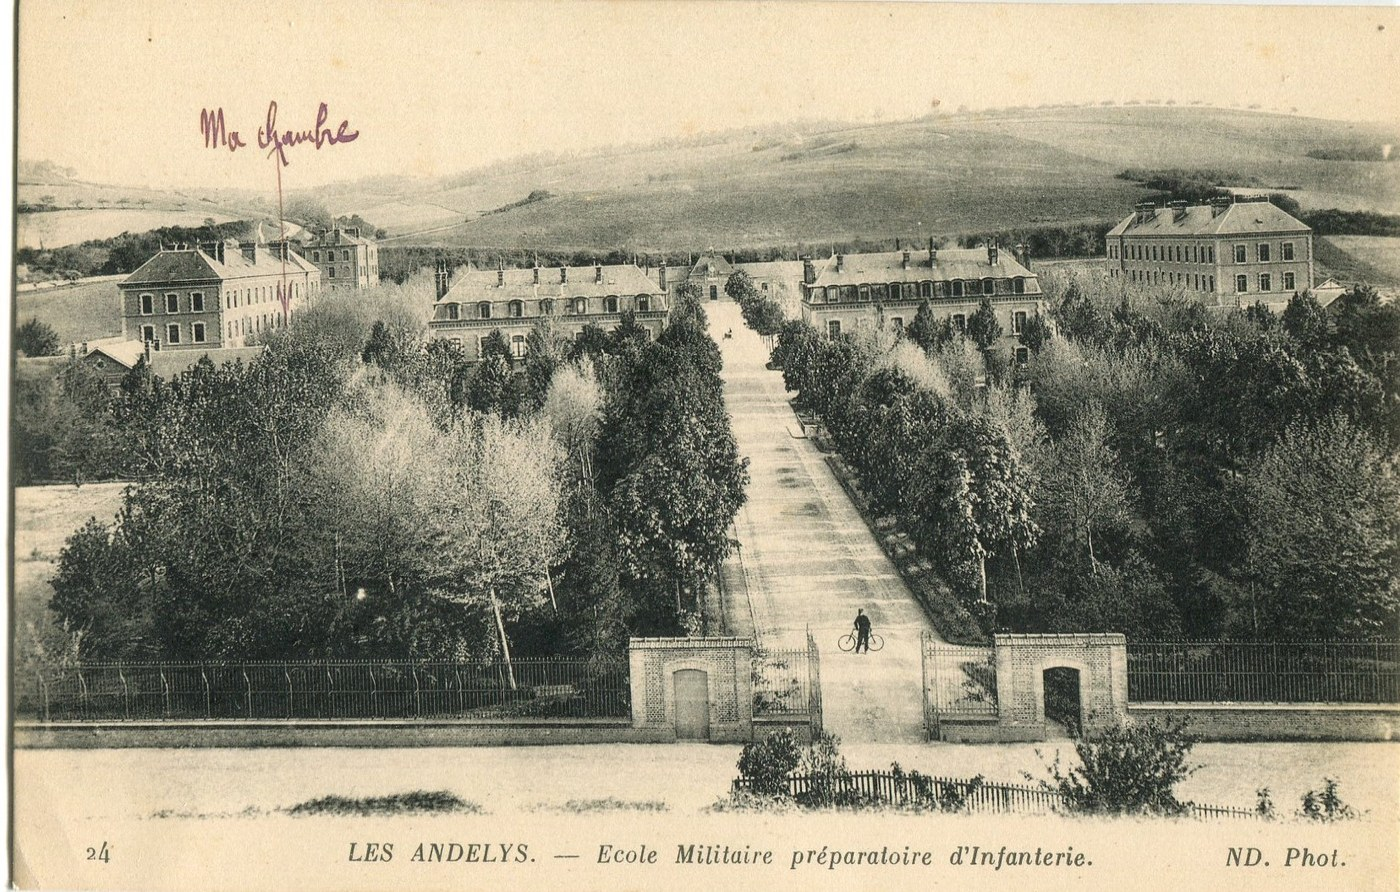
\includegraphics[width=0.94\linewidth,height=22mm,keepaspectratio]{illustrations/andelys_ecole_militaire.jpg}}
    \par\vspace{0.6mm}{\fontsize{5.8pt}{6.7pt}\selectfont Photographie de groupe devant l'École militaire préparatoire des Andelys (où Hippolyte est nommé professeur d'anglais le 24 novembre 1918).}
  \end{minipage}\hfill
  \begin{minipage}[b]{0.31\textwidth}
    \centering
    \setlength{\fboxsep}{0.7mm}\setlength{\fboxrule}{0.4pt}%
    \fcolorbox{gray!55}{white}{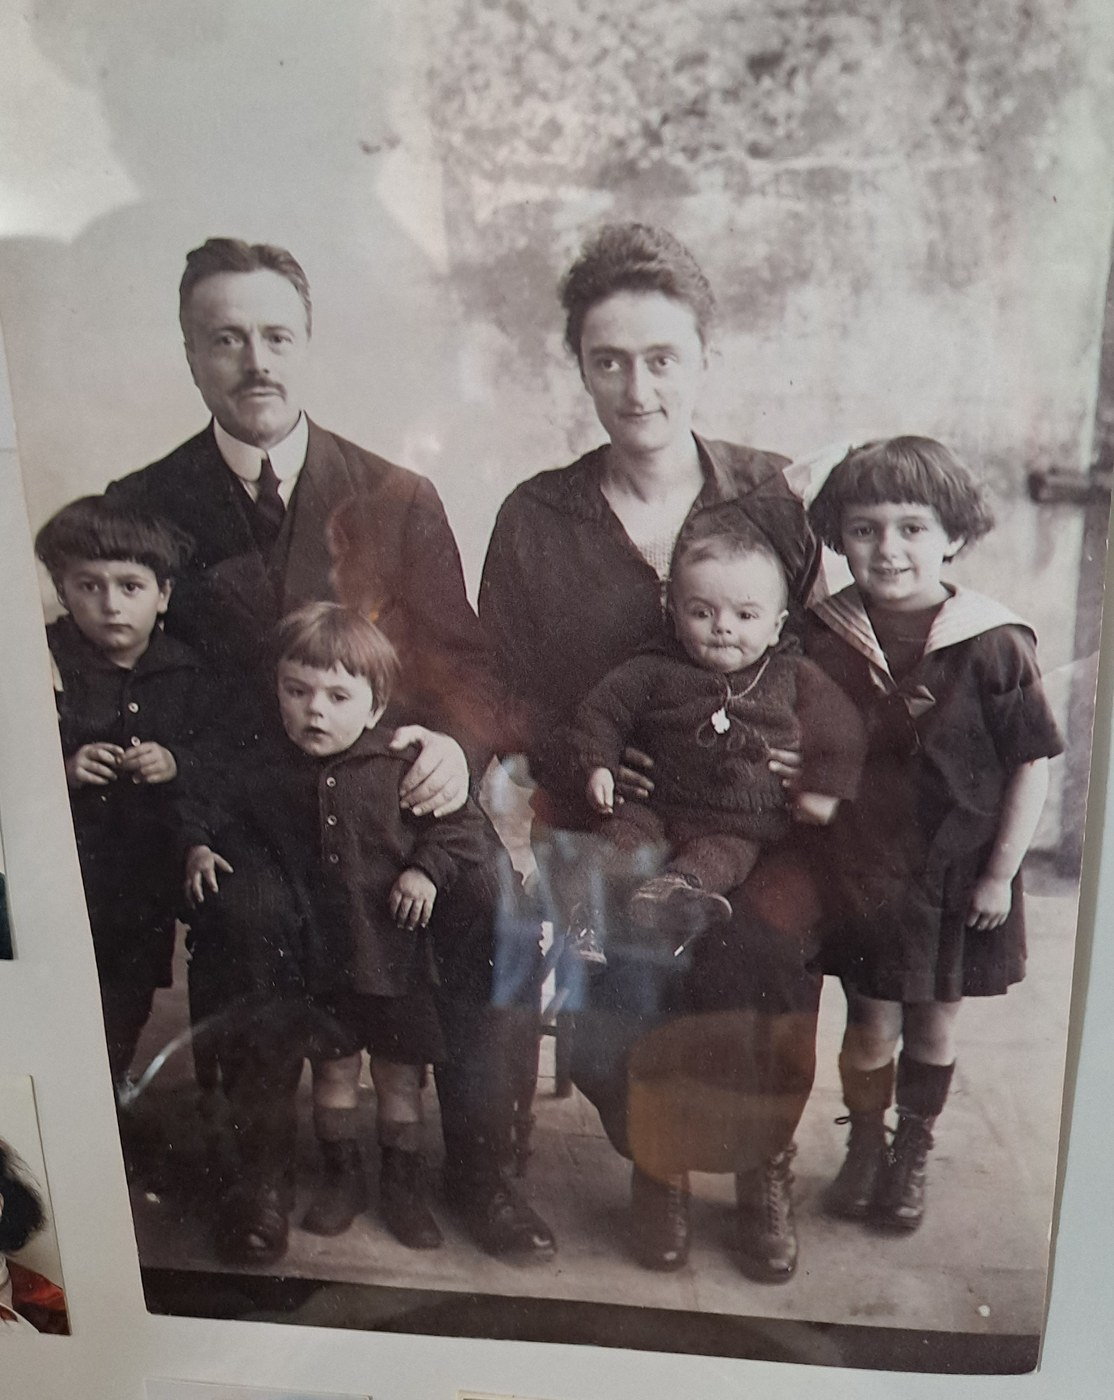
\includegraphics[width=0.94\linewidth,height=22mm,keepaspectratio]{illustrations/famille_combes_1925.jpg}}
    \par\vspace{0.6mm}{\fontsize{5.8pt}{6.7pt}\selectfont Hippolyte et Marguerite Combes entourés de leurs enfants à Montauban / Millau vers 1925.}
  \end{minipage}\hfill
  \begin{minipage}[b]{0.31\textwidth}
    \centering
    \setlength{\fboxsep}{0.7mm}\setlength{\fboxrule}{0.4pt}%
    \fcolorbox{gray!55}{white}{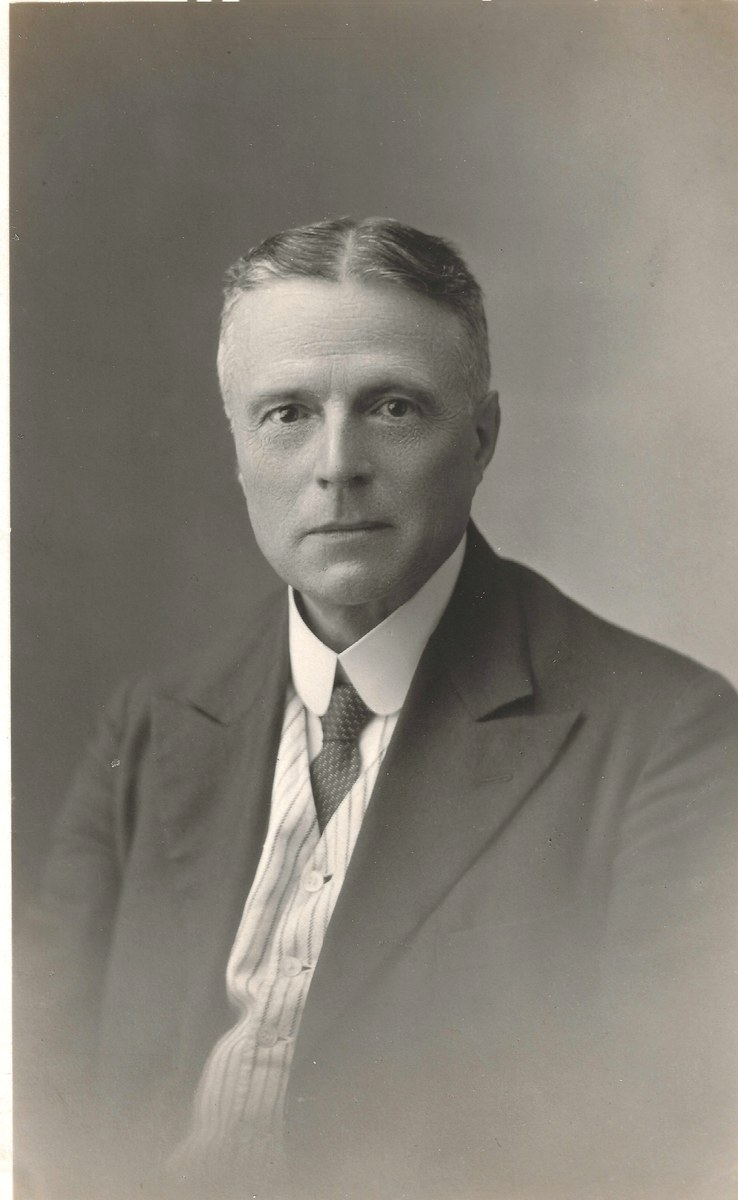
\includegraphics[width=0.94\linewidth,height=22mm,keepaspectratio]{illustrations/hippolyte_cambridge_1930.jpg}}
    \par\vspace{0.6mm}{\fontsize{5.8pt}{6.7pt}\selectfont Hippolyte Combes en Angleterre (Cambridge, été 1930).}
  \end{minipage}
\end{center}
\clearpage

% =============================================================================
% VIS-A-VIS SPREAD : SCAN #147 (20251126_110628.jpg) — Vue 147
% =============================================================================
\cleardoubleevenpage
% --- En-tête du folio (Page paire / gauche : Transcription, apparat & double registre) ---
\noindent\rule{\textwidth}{0.5pt}\par\vspace{0.6mm}
\noindent\textbf{\footnotesize SCAN \#147 — VUE 147} \hfill {\scriptsize\texttt{20251126\_\allowbreak 110628.jpg}}\par\vspace{0.3mm}
\noindent{\fontsize{7.0pt}{8.2pt}\selectfont Déménagement imprévu d'Acheux à Hérissart sous un gel intense}\par\vspace{0.25mm}
\noindent{\fontsize{7.0pt}{8.2pt}\selectfont\textit{7 février 1917 (après-midi)} \hfill \textit{Acheux, Raincheval, Puchevillers, Hérissart (Somme)}}\par\vspace{0.6mm}
\noindent\rule{\textwidth}{0.35pt}\par\vspace{1.0mm}
% --- Corps de la transcription diplomatique et apparat marginal en prolongement ---
{\renewcommand{\arraystretch}{0.95}%
\noindent\hspace*{3.5mm}\begin{tabular}{@{}p{100mm}@{\hspace{3.5mm}}p{55mm}@{}}
      \leavevmode\fontsize{7.4pt}{8.6pt}\selectfont\strut Merc. 7 (suite) \hfill{} Février 1917\strut & \leavevmode\fontsize{6.3pt}{7.2pt}\selectfont\raggedright\arraybackslash\color{black!88}\textbf{1} \textbf{Merc.} \textit{mercredi}. \\
      \leavevmode\fontsize{7.4pt}{8.6pt}\selectfont\strut En me rendant à notre office,\strut & \leavevmode\fontsize{6.3pt}{7.2pt}\selectfont\raggedright\arraybackslash\color{black!88}\textbf{2} \textbf{office} \textit{angl.} Bureau, anglais. \\
      \leavevmode\fontsize{7.4pt}{8.6pt}\selectfont\strut Mme Delille, qui au guichet, m'a appelé et\strut & \leavevmode\fontsize{6.3pt}{7.2pt}\selectfont\raggedright\arraybackslash\color{black!88}\textbf{3} \textbf{Mme} \textit{Madame}. \\
      \leavevmode\fontsize{7.4pt}{8.6pt}\selectfont\strut m'a appris que Cap. Williams, quitté Acheux\strut & \leavevmode\fontsize{6.3pt}{7.2pt}\selectfont\raggedright\arraybackslash\color{black!88}\textbf{4} \textbf{Cap. Williams} \textit{capitaine Williams}. \\
      \leavevmode\llap{\fontsize{6.5pt}{7.5pt}\selectfont\color{darkgray}5\hspace{1.8mm}}\fontsize{7.4pt}{8.6pt}\selectfont\strut pour $[\![$...$]\!]$ Hérissart. Venu aussitôt Mission\strut & \leavevmode\fontsize{6.3pt}{7.2pt}\selectfont\raggedright\arraybackslash\color{black!88}\textbf{5} \textbf{$[\![$...$]\!]$} Groupe annulé par un épais passage de plume avant Hérissart ; lecture sous la biffure non établie. \\
      \leavevmode\fontsize{7.4pt}{8.6pt}\selectfont\strut française, où trouvé un mot du Cap. W.\strut & \leavevmode\fontsize{6.3pt}{7.2pt}\selectfont\raggedright\arraybackslash\color{black!88}\textbf{6} \textbf{Cap. W.} \textit{capitaine Williams ; W. reprend le nom écrit l. 4}. \\
      \leavevmode\fontsize{7.4pt}{8.6pt}\selectfont\strut Lui ai téléphoné du bureau Mission pour lui\strut &  \\
      \leavevmode\fontsize{7.4pt}{8.6pt}\selectfont\strut annoncer mon arrivée.\strut &  \\
      \leavevmode\fontsize{7.4pt}{8.6pt}\selectfont\strut Rentré chez les Carluvant, auxquels annoncé mon\strut &  \\
      \leavevmode\llap{\fontsize{6.5pt}{7.5pt}\selectfont\color{darkgray}10\hspace{1.8mm}}\fontsize{7.4pt}{8.6pt}\selectfont\strut départ. Atterrés. Fait en hâte mes paquets. Attendu\strut &  \\
      \leavevmode\fontsize{7.4pt}{8.6pt}\selectfont\strut l'auto, qui arrivée vers 4h 1/2.\strut &  \\
      \leavevmode\fontsize{7.4pt}{8.6pt}\selectfont\strut Quitté village d'Acheux et surtout maison\strut &  \\
      \leavevmode\fontsize{7.4pt}{8.6pt}\selectfont\strut avec 1 serrement de cœur — —\strut &  \\
      \leavevmode\fontsize{7.4pt}{8.6pt}\selectfont\strut En auto à Hérissart, par Raincheval\strut &  \\
      \leavevmode\llap{\fontsize{6.5pt}{7.5pt}\selectfont\color{darkgray}15\hspace{1.8mm}}\fontsize{7.4pt}{8.6pt}\selectfont\strut \& Puchevillers.\strut &  \\
      \leavevmode\fontsize{7.4pt}{8.6pt}\selectfont\strut Bise glaciale. Froid intense.\strut &  \\
      \leavevmode\fontsize{7.4pt}{8.6pt}\selectfont\strut Town Major m'a donné petite chambre, n° 7b,\strut & \leavevmode\fontsize{6.3pt}{7.2pt}\selectfont\raggedright\arraybackslash\color{black!88}\textbf{17} \textbf{Town Major} \textit{angl.} Officier commandant la place ou le cantonnement, dans l’armée britannique. \\
      \leavevmode\fontsize{7.4pt}{8.6pt}\selectfont\strut 1er étage café Charlet, angle rue. De ma\strut &  \\
      \leavevmode\fontsize{7.4pt}{8.6pt}\selectfont\strut fenêtre, as. belle vue sur la place et église.\strut & \leavevmode\fontsize{6.3pt}{7.2pt}\selectfont\raggedright\arraybackslash\color{black!88}\textbf{19} \textbf{as.} \textit{assez}. \\
      \leavevmode\llap{\fontsize{6.5pt}{7.5pt}\selectfont\color{darkgray}20\hspace{1.8mm}}\fontsize{7.4pt}{8.6pt}\selectfont\strut Pleine lune brillait entre gds arbres.\strut & \leavevmode\fontsize{6.3pt}{7.2pt}\selectfont\raggedright\arraybackslash\color{black!88}\textbf{20} \textbf{gds} \textit{grands}. \\
      \leavevmode\fontsize{7.4pt}{8.6pt}\selectfont\strut Changement plutôt pénible d'habitudes.\strut &  \\
\end{tabular}}%
\par\vspace*{\fill}
% --- Deux registres de commentaires en bas de page (sans intitulés, distingués par filets et mise en page) ---
\noindent\rule{\textwidth}{0.5pt}\par\vspace{0.8mm}
{\fontsize{6.8pt}{8.0pt}\selectfont%
\noindent\normalfont l. 4 : une séparation précède « quitté Acheux », sans auxiliaire a distinct ; cette ellipse est conservée. l. 5 : groupe annulé par un épais passage de plume entre pour et Hérissart ; aucun texte antérieur assuré n’est proposé. l. 6 : W. reprend Williams, nommé l. 4 ; une seule note développe l’ensemble Cap. W., sans répéter Cap. l. 17 : Town Major est le titre britannique de l’officier chargé de la place ou du cantonnement. l. 12–13 : le « serrement de cœur » est explicitement écrit, sans qu’il soit nécessaire d’ajouter une interprétation affective à l’appareil de lecture.\par\vspace{0.75mm}
\noindent\rule{38mm}{0.4pt}\par\vspace{0.65mm}
\noindent\hspace*{5mm}\parbox{\dimexpr\textwidth-5mm\relax}{\fontsize{6.8pt}{8.0pt}\selectfont\color{black!82}\textbf{l.~2--21 :} Mme Delille annonce le départ de Williams ; un mot du capitaine l’attend à la Mission. Adieux aux Carluvant, parcours par Raincheval et Puchevillers, puis chambre 7 b au premier étage du café Charlet, avec vue sur place et église. Le texte ne nomme pas cette église et ne décrit pas un ordre administratif de transfert du bureau.}\par}
\newpage
% --- En-tête du fac-similé (Page impaire / droite : Scan original) ---
\noindent\rule{\textwidth}{0.5pt}\par\vspace{0.6mm}
\noindent\textbf{\fontsize{6.5pt}{7.6pt}\selectfont FAC-SIMILÉ EN VIS-À-VIS — VUE 147 (SCAN \#147)} \hfill {\fontsize{6.5pt}{7.6pt}\selectfont\texttt{20251126\_\allowbreak 110628.jpg}}\par\vspace{0.3mm}
\noindent{\fontsize{6.8pt}{8pt}\selectfont\textit{Livre-Journal d'Hippolyte Combes} — 7 février 1917 (après-midi) (Acheux, Raincheval, Puchevillers, Hérissart (Somme))}\par\vspace{0.6mm}
\noindent\rule{\textwidth}{0.35pt}\par\vspace*{\fill}
{\centering
  \setlength{\fboxsep}{1.2mm}%
  \setlength{\fboxrule}{0.4pt}%
  \fcolorbox{gray!55}{white}{%
    \includegraphics[width=0.94\textwidth,height=0.76\textheight,keepaspectratio]{\facsimiledir/20251126_110628.jpg}%
  }\par}
\vspace*{\fill}
\noindent\rule{\textwidth}{0.35pt}\par\vspace{0.5mm}
\noindent{\fontsize{6pt}{7.1pt}\selectfont\raggedright\color{darkgray}\textbf{Source :} Archives familiales Combes — Cliché numérique \texttt{20251126\_\allowbreak 110628.jpg} (Scan \#147/186, Vue 147). Haute définition : \texttt{scans\_haute\_qualite/\allowbreak 20251126\_\allowbreak 110628.jpg} ; version allégée : \texttt{scans\_compresses/\allowbreak 20251126\_\allowbreak 110628.jpg}.\par}
\newpage

% =============================================================================
% VIS-A-VIS SPREAD : SCAN #148 (20251126_110646.jpg) — Vue 148
% =============================================================================
\cleardoubleevenpage
% --- En-tête du folio (Page paire / gauche : Transcription, apparat & double registre) ---
\noindent\rule{\textwidth}{0.5pt}\par\vspace{0.6mm}
\noindent\textbf{\footnotesize SCAN \#148 — VUE 148} \hfill {\scriptsize\texttt{20251126\_\allowbreak 110646.jpg}}\par\vspace{0.3mm}
\noindent{\fontsize{7.0pt}{8.2pt}\selectfont Nuit glaciale à Hérissart, comptes de retour et premier jeudi de repos}\par\vspace{0.25mm}
\noindent{\fontsize{7.0pt}{8.2pt}\selectfont\textit{7 (fin) – 8 février 1917} \hfill \textit{Hérissart (Somme)}}\par\vspace{0.6mm}
\noindent\rule{\textwidth}{0.35pt}\par\vspace{1.0mm}
% --- Corps de la transcription diplomatique et apparat marginal en prolongement ---
{\renewcommand{\arraystretch}{1.02}%
\noindent\hspace*{3.5mm}\begin{tabular}{@{}p{100mm}@{\hspace{3.5mm}}p{55mm}@{}}
      \leavevmode\fontsize{7.8pt}{9.2pt}\selectfont\strut Merc. 7 (fin) \hfill{} Février 1917\strut & \leavevmode\fontsize{6.3pt}{7.2pt}\selectfont\raggedright\arraybackslash\color{black!88}\textbf{1} \textbf{Merc.} \textit{mercredi}. \\
      \leavevmode\fontsize{7.8pt}{9.2pt}\selectfont\strut Notre bureau \& mess, au n° 104, mauvaise\strut & \leavevmode\fontsize{6.3pt}{7.2pt}\selectfont\raggedright\arraybackslash\color{black!88}\textbf{2} \textbf{mess} \textit{angl.} Salle commune et service des repas des officiers, anglais. \\
      \leavevmode\fontsize{7.8pt}{9.2pt}\selectfont\strut installation.\strut &  \\
      \leavevmode\fontsize{7.8pt}{9.2pt}\selectfont\strut Après dîner, retourné chambre vers 9h.\strut &  \\
      \leavevmode\llap{\fontsize{6.5pt}{7.5pt}\selectfont\color{darkgray}5\hspace{1.8mm}}\fontsize{7.8pt}{9.2pt}\selectfont\strut Vitres recouvertes très épaisse gelée glacée.\strut &  \\
      \leavevmode\fontsize{7.8pt}{9.2pt}\selectfont\strut Froid extrt rigoureux.\strut & \leavevmode\fontsize{6.3pt}{7.2pt}\selectfont\raggedright\arraybackslash\color{black!88}\textbf{6} \textbf{extrt} \textit{extrêmement}. \\
      \leavevmode\fontsize{7.8pt}{9.2pt}\selectfont\strut [ Dîner à Paris, métro : 1 f.\strut & \leavevmode\fontsize{6.3pt}{7.2pt}\selectfont\raggedright\arraybackslash\color{black!88}\textbf{7} \textbf{[ Dîner} Grand crochet autographe à gauche du bloc de comptes ; les comptes occupent le milieu de la page sous le récit du mercredi. \\
      \leavevmode\fontsize{7.8pt}{9.2pt}\selectfont\strut Amiens, Y.M.C.A. : 1 f. 15 c.\strut & \leavevmode\fontsize{6.3pt}{7.2pt}\selectfont\raggedright\arraybackslash\color{black!88}\textbf{8} \textbf{Y.M.C.A.} \textit{Young Men’s Christian Association : association chrétienne de jeunes hommes}. \\
      \leavevmode\fontsize{7.8pt}{9.2pt}\selectfont\strut Touché solde Mission fr., Acheux : 78 f. 75\strut & \leavevmode\fontsize{6.3pt}{7.2pt}\selectfont\raggedright\arraybackslash\color{black!88}\textbf{9} \textbf{fr.} \textit{française, accordée avec Mission}. \\
      \leavevmode\llap{\fontsize{6.5pt}{7.5pt}\selectfont\color{darkgray}10\hspace{1.8mm}}\fontsize{7.8pt}{9.2pt}\selectfont\strut Gift aux Carluvant, pour\strut & \leavevmode\fontsize{6.3pt}{7.2pt}\selectfont\raggedright\arraybackslash\color{black!88}\textbf{10} \textbf{Gift} \textit{angl.} Don ou gratification, anglais. \\
      \leavevmode\fontsize{7.8pt}{9.2pt}\selectfont\strut mon lunch et room : 5 f. ]\strut & \leavevmode\fontsize{6.3pt}{7.2pt}\selectfont\raggedright\arraybackslash\color{black!88}\textbf{11} \textbf{lunch} \textit{angl.} Repas de midi, anglais ; \textbf{room} \textit{angl.} Chambre, anglais ; \textbf{et room} Ajout sous mon lunch, rattachant au paiement de 5 francs le repas et la chambre. \\
      \leavevmode\fontsize{7.8pt}{9.2pt}\selectfont\strut Jeudi 8.\strut & \leavevmode\fontsize{6.3pt}{7.2pt}\selectfont\raggedright\arraybackslash\color{black!88}\textbf{12} \textbf{Jeudi 8.} Nouvelle entrée de journal, séparée des comptes précédents par un long trait horizontal. \\
      \leavevmode\fontsize{7.8pt}{9.2pt}\selectfont\strut Très bonne nuit. Bien reposé. Lit\strut &  \\
      \leavevmode\fontsize{7.8pt}{9.2pt}\selectfont\strut très confortable.\strut &  \\
      \leavevmode\llap{\fontsize{6.5pt}{7.5pt}\selectfont\color{darkgray}15\hspace{1.8mm}}\fontsize{7.8pt}{9.2pt}\selectfont\strut Levé vers 8h —\strut &  \\
      \leavevmode\fontsize{7.8pt}{9.2pt}\selectfont\strut Soleil sur mes fenêtres.\strut &  \\
      \leavevmode\fontsize{7.8pt}{9.2pt}\selectfont\strut Descendu à l'office \& mess. Excellent\strut & \leavevmode\fontsize{6.3pt}{7.2pt}\selectfont\raggedright\arraybackslash\color{black!88}\textbf{17} \textbf{office} \textit{angl.} Bureau, anglais ; \textbf{mess} \textit{angl.} Salle commune et service des repas des officiers, anglais. \\
      \leavevmode\fontsize{7.8pt}{9.2pt}\selectfont\strut breakfast.\strut & \leavevmode\fontsize{6.3pt}{7.2pt}\selectfont\raggedright\arraybackslash\color{black!88}\textbf{18} \textbf{breakfast} \textit{angl.} Petit déjeuner, anglais. \\
      \leavevmode\fontsize{7.8pt}{9.2pt}\selectfont\strut Tout le jour, liberté entière —\strut &  \\
\end{tabular}}%
\par\vspace*{\fill}
% --- Deux registres de commentaires en bas de page (sans intitulés, distingués par filets et mise en page) ---
\noindent\rule{\textwidth}{0.5pt}\par\vspace{0.8mm}
{\fontsize{6.8pt}{8.0pt}\selectfont%
\noindent\normalfont l. 7–11 : bloc de comptes réuni par un grand crochet autographe à gauche, au milieu de la page. « et room » est ajouté sous « mon lunch » : le paiement de 5 francs concerne le repas et la chambre. La solde portée est 78 f 75 ; aucune décomposition de la somme n’est écrite. l. 11–12 : long trait horizontal séparant les comptes du mercredi et l’entrée Jeudi 8. Les termes anglais mess, Gift, lunch, room, office et breakfast sont traduits en marge ; les unités monétaires usuelles relèvent des conventions.\par\vspace{0.75mm}
\noindent\rule{38mm}{0.4pt}\par\vspace{0.65mm}
\noindent\hspace*{5mm}\parbox{\dimexpr\textwidth-5mm\relax}{\fontsize{6.8pt}{8.0pt}\selectfont\color{black!82}\textbf{l.~2--18 :} Bureau et mess au 104 ; les comptes portent solde de 78 f 75 et cadeau de 5 f aux Carluvant pour mon lunch, avec et room ajouté au-dessous. Le 19 février, la propriétaire du 104 sera dite malade au Scan 157 ; cette page ne fixe pas la date d’un futur emménagement ni la composition de la solde.}\par}
\newpage
% --- En-tête du fac-similé (Page impaire / droite : Scan original) ---
\noindent\rule{\textwidth}{0.5pt}\par\vspace{0.6mm}
\noindent\textbf{\fontsize{6.5pt}{7.6pt}\selectfont FAC-SIMILÉ EN VIS-À-VIS — VUE 148 (SCAN \#148)} \hfill {\fontsize{6.5pt}{7.6pt}\selectfont\texttt{20251126\_\allowbreak 110646.jpg}}\par\vspace{0.3mm}
\noindent{\fontsize{6.8pt}{8pt}\selectfont\textit{Livre-Journal d'Hippolyte Combes} — 7 (fin) – 8 février 1917 (Hérissart (Somme))}\par\vspace{0.6mm}
\noindent\rule{\textwidth}{0.35pt}\par\vspace*{\fill}
{\centering
  \setlength{\fboxsep}{1.2mm}%
  \setlength{\fboxrule}{0.4pt}%
  \fcolorbox{gray!55}{white}{%
    \includegraphics[width=0.94\textwidth,height=0.76\textheight,keepaspectratio]{\facsimiledir/20251126_110646.jpg}%
  }\par}
\vspace*{\fill}
\noindent\rule{\textwidth}{0.35pt}\par\vspace{0.5mm}
\noindent{\fontsize{6pt}{7.1pt}\selectfont\raggedright\color{darkgray}\textbf{Source :} Archives familiales Combes — Cliché numérique \texttt{20251126\_\allowbreak 110646.jpg} (Scan \#148/186, Vue 148). Haute définition : \texttt{scans\_haute\_qualite/\allowbreak 20251126\_\allowbreak 110646.jpg} ; version allégée : \texttt{scans\_compresses/\allowbreak 20251126\_\allowbreak 110646.jpg}.\par}
\newpage

% =============================================================================
% VIS-A-VIS SPREAD : SCAN #149 (20251126_110659.jpg) — Vue 149
% =============================================================================
\cleardoubleevenpage
% --- En-tête du folio (Page paire / gauche : Transcription, apparat & double registre) ---
\noindent\rule{\textwidth}{0.5pt}\par\vspace{0.6mm}
\noindent\textbf{\footnotesize SCAN \#149 — VUE 149} \hfill {\scriptsize\texttt{20251126\_\allowbreak 110659.jpg}}\par\vspace{0.3mm}
\noindent{\fontsize{7.0pt}{8.2pt}\selectfont Promenade à pied sur la neige durcie jusqu'à Rubempré}\par\vspace{0.25mm}
\noindent{\fontsize{7.0pt}{8.2pt}\selectfont\textit{8 (suite) – 9 février 1917 (matin)} \hfill \textit{Hérissart, Rubempré (Somme)}}\par\vspace{0.6mm}
\noindent\rule{\textwidth}{0.35pt}\par\vspace{1.0mm}
% --- Corps de la transcription diplomatique et apparat marginal en prolongement ---
{\renewcommand{\arraystretch}{1.02}%
\noindent\hspace*{3.5mm}\begin{tabular}{@{}p{100mm}@{\hspace{3.5mm}}p{55mm}@{}}
      \leavevmode\fontsize{7.8pt}{9.2pt}\selectfont\strut Jeudi 8 (suite) \hfill{} Février 1917\strut &  \\
      \leavevmode\fontsize{7.8pt}{9.2pt}\selectfont\strut Temps mervt beau. Ciel bleu, soleil ardent.\strut & \leavevmode\fontsize{6.3pt}{7.2pt}\selectfont\raggedright\arraybackslash\color{black!88}\textbf{2} \textbf{mervt} \textit{merveilleusement}. \\
      \leavevmode\fontsize{7.8pt}{9.2pt}\selectfont\strut Gelé très fort. Terre durcie, j'à gde profondeur.\strut & \leavevmode\fontsize{6.3pt}{7.2pt}\selectfont\raggedright\arraybackslash\color{black!88}\textbf{3} \textbf{j'à} \textit{jusqu’à} ; \textbf{gde} \textit{grande}. \\
      \leavevmode\fontsize{7.8pt}{9.2pt}\selectfont\strut Après-midi, promenade à pied à Rubempré.\strut &  \\
      \leavevmode\llap{\fontsize{6.5pt}{7.5pt}\selectfont\color{darkgray}5\hspace{1.8mm}}\fontsize{7.8pt}{9.2pt}\selectfont\strut Rayons ardents faisaient étinceler neige durcie,\strut &  \\
      \leavevmode\fontsize{7.8pt}{9.2pt}\selectfont\strut qui recouvrait champs.\strut &  \\
      \leavevmode\fontsize{7.8pt}{9.2pt}\selectfont\strut Région, moins banale qu'environs d'Acheux :\strut &  \\
      \leavevmode\fontsize{7.8pt}{9.2pt}\selectfont\strut vallonnements, petites hauteurs, couronnées de\strut &  \\
      \leavevmode\fontsize{7.8pt}{9.2pt}\selectfont\strut moulins à vent.\strut &  \\
      \leavevmode\llap{\fontsize{6.5pt}{7.5pt}\selectfont\color{darkgray}10\hspace{1.8mm}}\fontsize{7.8pt}{9.2pt}\selectfont\strut [durée incertaine] de marche.\strut & \leavevmode\fontsize{6.3pt}{7.2pt}\selectfont\raggedright\arraybackslash\color{black!88}\textbf{10} \textbf{[durée incertaine]} Notation de durée avant de marche ; chiffre et fraction éventuelle insuffisamment distincts pour une restitution assurée. \\
      \leavevmode\fontsize{7.8pt}{9.2pt}\selectfont\strut 1 h. ds ma chambre, où tt rangé et\strut & \leavevmode\fontsize{6.3pt}{7.2pt}\selectfont\raggedright\arraybackslash\color{black!88}\textbf{11} \textbf{ds} \textit{dans} ; \textbf{tt} \textit{tout}. \\
      \leavevmode\fontsize{7.8pt}{9.2pt}\selectfont\strut terminé installation.\strut &  \\
      \leavevmode\fontsize{7.8pt}{9.2pt}\selectfont\strut Froid toujours très vif.\strut &  \\
      \leavevmode\fontsize{7.8pt}{9.2pt}\selectfont\strut Couché vers 9h s. — 1 peu de lecture, lit\strut &  \\
      \leavevmode\llap{\fontsize{6.5pt}{7.5pt}\selectfont\color{darkgray}15\hspace{1.8mm}}\fontsize{7.8pt}{9.2pt}\selectfont\strut Ven. 9 — Nuit toujours excessvt froide.\strut & \leavevmode\fontsize{6.3pt}{7.2pt}\selectfont\raggedright\arraybackslash\color{black!88}\textbf{15} \textbf{Ven.} \textit{vendredi} ; \textbf{excessvt} \textit{excessivement} ; \textbf{Ven. 9} Nouvelle entrée, sous un trait horizontal autographe séparant les deux journées. \\
      \leavevmode\fontsize{7.8pt}{9.2pt}\selectfont\strut Gelé très fort. Ciel clair, pleine lune,\strut &  \\
      \leavevmode\fontsize{7.8pt}{9.2pt}\selectfont\strut vif éclat.\strut &  \\
      \leavevmode\fontsize{7.8pt}{9.2pt}\selectfont\strut Matinée, liberté complète. Mais trop froid\strut &  \\
      \leavevmode\fontsize{7.8pt}{9.2pt}\selectfont\strut pour pouvoir écrire chambre.\strut &  \\
\end{tabular}}%
\par\vspace*{\fill}
% --- Deux registres de commentaires en bas de page (sans intitulés, distingués par filets et mise en page) ---
\noindent\rule{\textwidth}{0.5pt}\par\vspace{0.8mm}
{\fontsize{6.8pt}{8.0pt}\selectfont%
\noindent\normalfont l. 3 : j’à gde développe jusqu’à grande, dans l’indication de profondeur du gel. l. 10 : la notation de durée précédant « de marche » reste non établie ; l’appareil ne la développe pas en une durée certaine. l. 15 : un trait horizontal sépare les entrées du jeudi et du vendredi. l. 18–19 : le froid empêche d’écrire dans la chambre ; le lieu de rédaction de cette page n’est pas précisé.\par\vspace{0.75mm}
\noindent\rule{38mm}{0.4pt}\par\vspace{0.65mm}
\noindent\hspace*{5mm}\parbox{\dimexpr\textwidth-5mm\relax}{\fontsize{6.8pt}{8.0pt}\selectfont\color{black!82}\textbf{l.~4--19 :} Promenade à Rubempré et description de vallonnements et moulins, puis rangement de la chambre. Le froid empêche d’y écrire le lendemain. La durée de marche est réservée ; première reconnaissance et caractère crayeux des reliefs sont des précisions extérieures au texte.}\par}
\newpage
% --- En-tête du fac-similé (Page impaire / droite : Scan original) ---
\noindent\rule{\textwidth}{0.5pt}\par\vspace{0.6mm}
\noindent\textbf{\fontsize{6.5pt}{7.6pt}\selectfont FAC-SIMILÉ EN VIS-À-VIS — VUE 149 (SCAN \#149)} \hfill {\fontsize{6.5pt}{7.6pt}\selectfont\texttt{20251126\_\allowbreak 110659.jpg}}\par\vspace{0.3mm}
\noindent{\fontsize{6.8pt}{8pt}\selectfont\textit{Livre-Journal d'Hippolyte Combes} — 8 (suite) – 9 février 1917 (matin) (Hérissart, Rubempré (Somme))}\par\vspace{0.6mm}
\noindent\rule{\textwidth}{0.35pt}\par\vspace*{\fill}
{\centering
  \setlength{\fboxsep}{1.2mm}%
  \setlength{\fboxrule}{0.4pt}%
  \fcolorbox{gray!55}{white}{%
    \includegraphics[width=0.94\textwidth,height=0.76\textheight,keepaspectratio]{\facsimiledir/20251126_110659.jpg}%
  }\par}
\vspace*{\fill}
\noindent\rule{\textwidth}{0.35pt}\par\vspace{0.5mm}
\noindent{\fontsize{6pt}{7.1pt}\selectfont\raggedright\color{darkgray}\textbf{Source :} Archives familiales Combes — Cliché numérique \texttt{20251126\_\allowbreak 110659.jpg} (Scan \#149/186, Vue 149). Haute définition : \texttt{scans\_haute\_qualite/\allowbreak 20251126\_\allowbreak 110659.jpg} ; version allégée : \texttt{scans\_compresses/\allowbreak 20251126\_\allowbreak 110659.jpg}.\par}
\newpage

% =============================================================================
% VIS-A-VIS SPREAD : SCAN #150 (20251126_110726.jpg) — Vue 150
% =============================================================================
\cleardoubleevenpage
% --- En-tête du folio (Page paire / gauche : Transcription, apparat & double registre) ---
\noindent\rule{\textwidth}{0.5pt}\par\vspace{0.6mm}
\noindent\textbf{\footnotesize SCAN \#150 — VUE 150} \hfill {\scriptsize\texttt{20251126\_\allowbreak 110726.jpg}}\par\vspace{0.3mm}
\noindent{\fontsize{7.0pt}{8.2pt}\selectfont Visite à la Mission de Toutencourt et course à Martinsart}\par\vspace{0.25mm}
\noindent{\fontsize{7.0pt}{8.2pt}\selectfont\textit{9 (suite) – 10 février 1917 (matin)} \hfill \textit{Hérissart, Toutencourt, Martinsart (Somme)}}\par\vspace{0.6mm}
\noindent\rule{\textwidth}{0.35pt}\par\vspace{1.0mm}
% --- Corps de la transcription diplomatique et apparat marginal en prolongement ---
{\renewcommand{\arraystretch}{0.95}%
\noindent\hspace*{3.5mm}\begin{tabular}{@{}p{100mm}@{\hspace{3.5mm}}p{55mm}@{}}
      \leavevmode\fontsize{7.4pt}{8.6pt}\selectfont\strut — Vendredi 9 (suite) — \hfill{} Février 1917\strut &  \\
      \leavevmode\fontsize{7.4pt}{8.6pt}\selectfont\strut Après-midi, ds l'auto du Lieutt Croughton,\strut & \leavevmode\fontsize{6.3pt}{7.2pt}\selectfont\raggedright\arraybackslash\color{black!88}\textbf{2} \textbf{ds} \textit{dans} ; \textbf{Lieutt} \textit{lieutenant}. \\
      \leavevmode\fontsize{7.4pt}{8.6pt}\selectfont\strut venu à Toutencourt. Bureau Mission fr. : appris\strut & \leavevmode\fontsize{6.3pt}{7.2pt}\selectfont\raggedright\arraybackslash\color{black!88}\textbf{3} \textbf{fr.} \textit{française, accordée avec Mission}. \\
      \leavevmode\fontsize{7.4pt}{8.6pt}\selectfont\strut que désormais serai administré par l'armée et\strut &  \\
      \leavevmode\llap{\fontsize{6.5pt}{7.5pt}\selectfont\color{darkgray}5\hspace{1.8mm}}\fontsize{7.4pt}{8.6pt}\selectfont\strut payé les 3 et 18 de chaque mois.\strut &  \\
      \leavevmode\fontsize{7.4pt}{8.6pt}\selectfont\strut Retour sur 1 lorry.\strut & \leavevmode\fontsize{6.3pt}{7.2pt}\selectfont\raggedright\arraybackslash\color{black!88}\textbf{6} \textbf{lorry} \textit{angl.} Camion, anglais. \\
      \leavevmode\fontsize{7.4pt}{8.6pt}\selectfont\strut Écrit salle café maison où chambre.\strut &  \\
      \leavevmode\fontsize{7.4pt}{8.6pt}\selectfont\strut Vers 6h s., avec Cap. W., ds les fermes\strut & \leavevmode\fontsize{6.3pt}{7.2pt}\selectfont\raggedright\arraybackslash\color{black!88}\textbf{8} \textbf{Cap. W.} \textit{capitaine Williams} ; \textbf{ds} \textit{dans}. \\
      \leavevmode\fontsize{7.4pt}{8.6pt}\selectfont\strut pour acheter paille \& foin.\strut &  \\
      \leavevmode\llap{\fontsize{6.5pt}{7.5pt}\selectfont\color{darkgray}10\hspace{1.8mm}}\fontsize{7.4pt}{8.6pt}\selectfont\strut Sam. 10.\strut & \leavevmode\fontsize{6.3pt}{7.2pt}\selectfont\raggedright\arraybackslash\color{black!88}\textbf{10} \textbf{Sam.} \textit{samedi} ; \textbf{Sam. 10.} Nouvelle entrée de journal, titre souligné et séparé du récit précédent par un espace. \\
      \leavevmode\fontsize{7.4pt}{8.6pt}\selectfont\strut Sur pied dès 7h.\strut &  \\
      \leavevmode\fontsize{7.4pt}{8.6pt}\selectfont\strut Dû sortir aussitôt pour aller aux Lignes de M.T.,\strut & \leavevmode\fontsize{6.3pt}{7.2pt}\selectfont\raggedright\arraybackslash\color{black!88}\textbf{12} \textbf{Lignes} \textit{Lignes : développement déjà adopté dans le texte ; le manuscrit porte L suivi d’une courte terminaison suscrite} ; \textbf{M.T.} \textit{Motor Transport : transport automobile, sigle militaire britannique}. \\
      \leavevmode\fontsize{7.4pt}{8.6pt}\selectfont\strut at the end of the road.\strut & \leavevmode\fontsize{6.3pt}{7.2pt}\selectfont\raggedright\arraybackslash\color{black!88}\textbf{13} \textbf{at the end of the road} \textit{angl.} Au bout de la route, anglais. \\
      \leavevmode\fontsize{7.4pt}{8.6pt}\selectfont\strut Nuit \& matinée, froid vif, très pénétrant.\strut &  \\
      \leavevmode\llap{\fontsize{6.5pt}{7.5pt}\selectfont\color{darkgray}15\hspace{1.8mm}}\fontsize{7.4pt}{8.6pt}\selectfont\strut Gelé toujours très fort.\strut &  \\
      \leavevmode\fontsize{7.4pt}{8.6pt}\selectfont\strut Après le breakfast, partis en auto à Martinsart.\strut & \leavevmode\fontsize{6.3pt}{7.2pt}\selectfont\raggedright\arraybackslash\color{black!88}\textbf{16} \textbf{breakfast} \textit{angl.} Petit déjeuner, anglais. \\
      \leavevmode\fontsize{7.4pt}{8.6pt}\selectfont\strut Dévalé routes en pente. Des 2 côtés, champs couverts\strut &  \\
      \leavevmode\fontsize{7.4pt}{8.6pt}\selectfont\strut de neige durcie. Soleil se lève, de + en + chaud.\strut &  \\
      \leavevmode\fontsize{7.4pt}{8.6pt}\selectfont\strut Au château de Martinsart, reçus par\strut &  \\
      \leavevmode\llap{\fontsize{6.5pt}{7.5pt}\selectfont\color{darkgray}20\hspace{1.8mm}}\fontsize{7.4pt}{8.6pt}\selectfont\strut un génal [Volké ?], très aimable.\strut & \leavevmode\fontsize{6.3pt}{7.2pt}\selectfont\raggedright\arraybackslash\color{black!88}\textbf{20} \textbf{génal} \textit{général} ; \textbf{[Volké ?]} Nom après génal de lecture incertaine ; Volké est une proposition graphique, sans identification certaine. \\
      \leavevmode\fontsize{7.4pt}{8.6pt}\selectfont\strut Village, rempli de troupes anglaises.\strut &  \\
\end{tabular}}%
\par\vspace*{\fill}
% --- Deux registres de commentaires en bas de page (sans intitulés, distingués par filets et mise en page) ---
\noindent\rule{\textwidth}{0.5pt}\par\vspace{0.8mm}
{\fontsize{6.8pt}{8.0pt}\selectfont%
\noindent\normalfont l. 7 : la phrase elliptique « Écrit salle café maison où chambre » est conservée ; elle ne contient pas de référence à un poêle. l. 12 : le manuscrit abrège Lignes par L et une courte terminaison suscrite, déjà développée dans la transcription ; M.T. vaut Motor Transport, « transport automobile ». l. 13 : courte proposition entièrement en anglais, « au bout de la route ». l. 20 : génal est une contraction de général ; le nom qui suit reste réservé. Le rapprochement militaire évoqué dans le commentaire historique ne constitue pas une preuve de lecture du nom.\par\vspace{0.75mm}
\noindent\rule{38mm}{0.4pt}\par\vspace{0.65mm}
\noindent\hspace*{5mm}\parbox{\dimexpr\textwidth-5mm\relax}{\fontsize{6.8pt}{8.0pt}\selectfont\color{black!82}\textbf{l.~2--21 :} Croughton[?] a déjà une occurrence à Authie au Scan 109 ; la comparaison est nominative, non une identification civile. Combes apprend à Toutencourt qu’il sera administré par l’armée et payé les 3 et 18. Les paiements des Scans 156, 162 et 170 fournissent des rapprochements internes. Le niveau administratif antérieur et le numéro de parc automobile ne sont pas précisés.}\par}
\newpage
% --- En-tête du fac-similé (Page impaire / droite : Scan original) ---
\noindent\rule{\textwidth}{0.5pt}\par\vspace{0.6mm}
\noindent\textbf{\fontsize{6.5pt}{7.6pt}\selectfont FAC-SIMILÉ EN VIS-À-VIS — VUE 150 (SCAN \#150)} \hfill {\fontsize{6.5pt}{7.6pt}\selectfont\texttt{20251126\_\allowbreak 110726.jpg}}\par\vspace{0.3mm}
\noindent{\fontsize{6.8pt}{8pt}\selectfont\textit{Livre-Journal d'Hippolyte Combes} — 9 (suite) – 10 février 1917 (matin) (Hérissart, Toutencourt, Martinsart (Somme))}\par\vspace{0.6mm}
\noindent\rule{\textwidth}{0.35pt}\par\vspace*{\fill}
{\centering
  \setlength{\fboxsep}{1.2mm}%
  \setlength{\fboxrule}{0.4pt}%
  \fcolorbox{gray!55}{white}{%
    \includegraphics[width=0.94\textwidth,height=0.76\textheight,keepaspectratio]{\facsimiledir/20251126_110726.jpg}%
  }\par}
\vspace*{\fill}
\noindent\rule{\textwidth}{0.35pt}\par\vspace{0.5mm}
\noindent{\fontsize{6pt}{7.1pt}\selectfont\raggedright\color{darkgray}\textbf{Source :} Archives familiales Combes — Cliché numérique \texttt{20251126\_\allowbreak 110726.jpg} (Scan \#150/186, Vue 150). Haute définition : \texttt{scans\_haute\_qualite/\allowbreak 20251126\_\allowbreak 110726.jpg} ; version allégée : \texttt{scans\_compresses/\allowbreak 20251126\_\allowbreak 110726.jpg}.\par}
\newpage

% =============================================================================
% VIS-A-VIS SPREAD : SCAN #151 (20251126_110737.jpg) — Vue 151
% =============================================================================
\cleardoubleevenpage
% --- En-tête du folio (Page paire / gauche : Transcription, apparat & double registre) ---
\noindent\rule{\textwidth}{0.5pt}\par\vspace{0.6mm}
\noindent\textbf{\footnotesize SCAN \#151 — VUE 151} \hfill {\scriptsize\texttt{20251126\_\allowbreak 110737.jpg}}\par\vspace{0.3mm}
\noindent{\fontsize{7.0pt}{8.2pt}\selectfont Visite à son ancienne compagnie au bois d'Aveluy et combat aérien}\par\vspace{0.25mm}
\noindent{\fontsize{7.0pt}{8.2pt}\selectfont\textit{10 (suite) – 11 février 1917 (matin)} \hfill \textit{Bois d'Aveluy, Senlis-le-Sec, Acheux, Hérissart (Somme)}}\par\vspace{0.6mm}
\noindent\rule{\textwidth}{0.35pt}\par\vspace{1.0mm}
% --- Corps de la transcription diplomatique et apparat marginal en prolongement ---
{\renewcommand{\arraystretch}{0.95}%
\noindent\hspace*{3.5mm}\begin{tabular}{@{}p{100mm}@{\hspace{3.5mm}}p{55mm}@{}}
      \leavevmode\fontsize{7.4pt}{8.6pt}\selectfont\strut Sam. 10 (suite) \hfill{} Février 1917\strut & \leavevmode\fontsize{6.3pt}{7.2pt}\selectfont\raggedright\arraybackslash\color{black!88}\textbf{1} \textbf{Sam.} \textit{samedi}. \\
      \leavevmode\fontsize{7.4pt}{8.6pt}\selectfont\strut Continué en auto route d'Aveluy, mon ancienne\strut &  \\
      \leavevmode\fontsize{7.4pt}{8.6pt}\selectfont\strut Cy, campée champ dévasté, sous des tentes.\strut & \leavevmode\fontsize{6.3pt}{7.2pt}\selectfont\raggedright\arraybackslash\color{black!88}\textbf{3} \textbf{Cy} \textit{Company : compagnie, anglais}. \\
      \leavevmode\fontsize{7.4pt}{8.6pt}\selectfont\strut Lunché au mess, où vu Lt Bradfield (très aimable).\strut & \leavevmode\fontsize{6.3pt}{7.2pt}\selectfont\raggedright\arraybackslash\color{black!88}\textbf{4} \textbf{Lunché} \textit{hybr.} Pris le repas de midi ; verbe français formé sur l’anglais lunch ; \textbf{mess} \textit{angl.} Salle commune et service des repas des officiers, anglais ; \textbf{Lt} \textit{lieutenant}. \\
      \leavevmode\llap{\fontsize{6.5pt}{7.5pt}\selectfont\color{darkgray}5\hspace{1.8mm}}\fontsize{7.4pt}{8.6pt}\selectfont\strut Puis visité cantonnemt et causé avec qq N.C.O's \& men.\strut & \leavevmode\fontsize{6.3pt}{7.2pt}\selectfont\raggedright\arraybackslash\color{black!88}\textbf{5} \textbf{cantonnemt} \textit{cantonnement} ; \textbf{qq} \textit{quelques} ; \textbf{N.C.O's} \textit{Non-Commissioned Officers : sous-officiers, anglais} ; \textbf{men} \textit{angl.} Soldats, hommes de troupe, anglais. \\
      \leavevmode\fontsize{7.4pt}{8.6pt}\selectfont\strut Ciel très bleu. Soleil brûlant. De ts côtés,\strut & \leavevmode\fontsize{6.3pt}{7.2pt}\selectfont\raggedright\arraybackslash\color{black!88}\textbf{6} \textbf{ts} \textit{tous}. \\
      \leavevmode\fontsize{7.4pt}{8.6pt}\selectfont\strut vastes horizons. Canons de marine, en batterie\strut &  \\
      \leavevmode\fontsize{7.4pt}{8.6pt}\selectfont\strut \& cachés sous des branchages desséchés.\strut &  \\
      \leavevmode\fontsize{7.4pt}{8.6pt}\selectfont\strut 2 avions boches, canonnés ds l'azur —\strut & \leavevmode\fontsize{6.3pt}{7.2pt}\selectfont\raggedright\arraybackslash\color{black!88}\textbf{9} \textbf{ds} \textit{dans}. \\
      \leavevmode\llap{\fontsize{6.5pt}{7.5pt}\selectfont\color{darkgray}10\hspace{1.8mm}}\fontsize{7.4pt}{8.6pt}\selectfont\strut Au retour, arrêté au refilling point, où revu\strut & \leavevmode\fontsize{6.3pt}{7.2pt}\selectfont\raggedright\arraybackslash\color{black!88}\textbf{10} \textbf{refilling point} \textit{angl.} Point de réapprovisionnement ou de ravitaillement, anglais. \\
      \leavevmode\fontsize{7.4pt}{8.6pt}\selectfont\strut Cap. Lovet. Charmant.\strut & \leavevmode\fontsize{6.3pt}{7.2pt}\selectfont\raggedright\arraybackslash\color{black!88}\textbf{11} \textbf{Cap.} \textit{capitaine}. \\
      \leavevmode\fontsize{7.4pt}{8.6pt}\selectfont\strut Rentrés vers 3h 1/2, par Senlis. A la miss. fr.\strut & \leavevmode\fontsize{6.3pt}{7.2pt}\selectfont\raggedright\arraybackslash\color{black!88}\textbf{12} \textbf{miss. fr.} \textit{mission française}. \\
      \leavevmode\fontsize{7.4pt}{8.6pt}\selectfont\strut 2e corps, vu Cap. de Casteljau, énorme \& bête.\strut & \leavevmode\fontsize{6.3pt}{7.2pt}\selectfont\raggedright\arraybackslash\color{black!88}\textbf{13} \textbf{Cap.} \textit{capitaine}. \\
      \leavevmode\fontsize{7.4pt}{8.6pt}\selectfont\strut Passé par Acheux.\strut &  \\
      \leavevmode\llap{\fontsize{6.5pt}{7.5pt}\selectfont\color{darkgray}15\hspace{1.8mm}}\fontsize{7.4pt}{8.6pt}\selectfont\strut Soleil rouge disparaissait à l'horizon.\strut &  \\
      \leavevmode\fontsize{7.4pt}{8.6pt}\selectfont\strut Nuit étoilée et sans lune.\strut &  \\
      \leavevmode\fontsize{7.4pt}{8.6pt}\selectfont\strut Dim. 11 — Nuit toujours très froide. Gelé\strut & \leavevmode\fontsize{6.3pt}{7.2pt}\selectfont\raggedright\arraybackslash\color{black!88}\textbf{17} \textbf{Dim.} \textit{dimanche}. \\
      \leavevmode\fontsize{7.4pt}{8.6pt}\selectfont\strut extrt fort.\strut & \leavevmode\fontsize{6.3pt}{7.2pt}\selectfont\raggedright\arraybackslash\color{black!88}\textbf{18} \textbf{extrt} \textit{extrêmement}. \\
      \leavevmode\fontsize{7.4pt}{8.6pt}\selectfont\strut Ds le 1/2 du jour, ardent soleil réchauffe\strut & \leavevmode\fontsize{6.3pt}{7.2pt}\selectfont\raggedright\arraybackslash\color{black!88}\textbf{19} \textbf{Ds} \textit{Dans} ; \textbf{1/2 du jour} Milieu du jour, dans ce contexte ; cette fraction graphique ne désigne pas ici une durée d’une demi-journée. \\
      \leavevmode\llap{\fontsize{6.5pt}{7.5pt}\selectfont\color{darkgray}20\hspace{1.8mm}}\fontsize{7.4pt}{8.6pt}\selectfont\strut sensiblement température. Bientôt ce sera\strut &  \\
      \leavevmode\fontsize{7.4pt}{8.6pt}\selectfont\strut le dégel, et fin de l'hiver.\strut &  \\
\end{tabular}}%
\par\vspace*{\fill}
% --- Deux registres de commentaires en bas de page (sans intitulés, distingués par filets et mise en page) ---
\noindent\rule{\textwidth}{0.5pt}\par\vspace{0.8mm}
{\fontsize{6.8pt}{8.0pt}\selectfont%
\noindent\normalfont l. 3–5 : les formes militaires anglaises Cy et N.C.O’s sont développées Company, « compagnie », et Non-Commissioned Officers, « sous-officiers » ; men désigne les hommes de troupe. Lunché est une formation verbale française sur lunch. l. 10 : refilling point désigne un point de réapprovisionnement, sans précision sur les unités desservies. l. 12 : miss. fr. abrège mission française. l. 19 : 1/2 du jour signifie ici le milieu de la journée, à distinguer d’une durée d’une demi-journée. L’entrée Dim. 11 est placée après un espace et un tiret initial.\par\vspace{0.75mm}
\noindent\rule{38mm}{0.4pt}\par\vspace{0.65mm}
\noindent\hspace*{5mm}\parbox{\dimexpr\textwidth-5mm\relax}{\fontsize{6.8pt}{8.0pt}\selectfont\color{black!82}\textbf{l.~2--14 :} L’ancienne Cy d’Aveluy, Bradfield, Lovet, le refilling point et la Mission du 2e Corps à Senlis sont nommés. Le Scan 066 donne 152 Coy A.S.C., mais le rapprochement avec cette ancienne compagnie ne doit pas remplacer la formule autographe. Portée des canons, fonction de Casteljau et secteur opérationnel du corps ne sont pas indiqués.}\par}
\newpage
% --- En-tête du fac-similé (Page impaire / droite : Scan original) ---
\noindent\rule{\textwidth}{0.5pt}\par\vspace{0.6mm}
\noindent\textbf{\fontsize{6.5pt}{7.6pt}\selectfont FAC-SIMILÉ EN VIS-À-VIS — VUE 151 (SCAN \#151)} \hfill {\fontsize{6.5pt}{7.6pt}\selectfont\texttt{20251126\_\allowbreak 110737.jpg}}\par\vspace{0.3mm}
\noindent{\fontsize{6.8pt}{8pt}\selectfont\textit{Livre-Journal d'Hippolyte Combes} — 10 (suite) – 11 février 1917 (matin) (Bois d'Aveluy, Senlis-le-Sec, Acheux, Hérissart (Somme))}\par\vspace{0.6mm}
\noindent\rule{\textwidth}{0.35pt}\par\vspace*{\fill}
{\centering
  \setlength{\fboxsep}{1.2mm}%
  \setlength{\fboxrule}{0.4pt}%
  \fcolorbox{gray!55}{white}{%
    \includegraphics[width=0.94\textwidth,height=0.76\textheight,keepaspectratio]{\facsimiledir/20251126_110737.jpg}%
  }\par}
\vspace*{\fill}
\noindent\rule{\textwidth}{0.35pt}\par\vspace{0.5mm}
\noindent{\fontsize{6pt}{7.1pt}\selectfont\raggedright\color{darkgray}\textbf{Source :} Archives familiales Combes — Cliché numérique \texttt{20251126\_\allowbreak 110737.jpg} (Scan \#151/186, Vue 151). Haute définition : \texttt{scans\_haute\_qualite/\allowbreak 20251126\_\allowbreak 110737.jpg} ; version allégée : \texttt{scans\_compresses/\allowbreak 20251126\_\allowbreak 110737.jpg}.\par}
\newpage

% =============================================================================
% VIS-A-VIS SPREAD : SCAN #152 (20251126_110753.jpg) — Vue 152
% =============================================================================
\cleardoubleevenpage
% --- En-tête du folio (Page paire / gauche : Transcription, apparat & double registre) ---
\noindent\rule{\textwidth}{0.5pt}\par\vspace{0.6mm}
\noindent\textbf{\footnotesize SCAN \#152 — VUE 152} \hfill {\scriptsize\texttt{20251126\_\allowbreak 110753.jpg}}\par\vspace{0.3mm}
\noindent{\fontsize{7.0pt}{8.2pt}\selectfont Excursion dominicale à Doullens et Auxi-le-Château chez M. Romert}\par\vspace{0.25mm}
\noindent{\fontsize{7.0pt}{8.2pt}\selectfont\textit{11 février 1917 (suite)} \hfill \textit{Toutencourt, Doullens, Auxi-le-Château (Somme / Pas-de-Calais)}}\par\vspace{0.6mm}
\noindent\rule{\textwidth}{0.35pt}\par\vspace{1.0mm}
% --- Corps de la transcription diplomatique et apparat marginal en prolongement ---
{\renewcommand{\arraystretch}{0.95}%
\noindent\hspace*{3.5mm}\begin{tabular}{@{}p{100mm}@{\hspace{3.5mm}}p{55mm}@{}}
      \leavevmode\fontsize{7.4pt}{8.6pt}\selectfont\strut Dim. 11 — \hfill{} — Février 1917 —\strut & \leavevmode\fontsize{6.3pt}{7.2pt}\selectfont\raggedright\arraybackslash\color{black!88}\textbf{1} \textbf{Dim.} \textit{dimanche}. \\
      \leavevmode\fontsize{7.4pt}{8.6pt}\selectfont\strut Tout le jour, en course.\strut &  \\
      \leavevmode\fontsize{7.4pt}{8.6pt}\selectfont\strut Matinée, à Toutencourt.\strut &  \\
      \leavevmode\fontsize{7.4pt}{8.6pt}\selectfont\strut Déjeuné à Doullens, où arrêt de 3 h.\strut &  \\
      \leavevmode\llap{\fontsize{6.5pt}{7.5pt}\selectfont\color{darkgray}5\hspace{1.8mm}}\fontsize{7.4pt}{8.6pt}\selectfont\strut Promenade solitaire à travers campagne, autour\strut &  \\
      \leavevmode\fontsize{7.4pt}{8.6pt}\selectfont\strut de la ville, le long d'1 petit ruisseau.\strut &  \\
      \leavevmode\fontsize{7.4pt}{8.6pt}\selectfont\strut Temps très beau.\strut &  \\
      \leavevmode\fontsize{7.4pt}{8.6pt}\selectfont\strut Continué, 3h s., jusqu'à Auxi-le-Château.\strut &  \\
      \leavevmode\fontsize{7.4pt}{8.6pt}\selectfont\strut Vu M. Romert. M'a offert café et excellent\strut &  \\
      \leavevmode\llap{\fontsize{6.5pt}{7.5pt}\selectfont\color{darkgray}10\hspace{1.8mm}}\fontsize{7.4pt}{8.6pt}\selectfont\strut rhum (1870) et kirsch Forêt Noire. Causé de\strut &  \\
      \leavevmode\fontsize{7.4pt}{8.6pt}\selectfont\strut tout un peu. Vieux célibataire, héritier de 3\strut &  \\
      \leavevmode\fontsize{7.4pt}{8.6pt}\selectfont\strut générations, laissera fortune à des étrangers.\strut &  \\
      \leavevmode\fontsize{7.4pt}{8.6pt}\selectfont\strut Au retour, soleil disparu, air de + en +\strut &  \\
      \leavevmode\fontsize{7.4pt}{8.6pt}\selectfont\strut glacé. Commence à geler très durement.\strut &  \\
      \leavevmode\llap{\fontsize{6.5pt}{7.5pt}\selectfont\color{darkgray}15\hspace{1.8mm}}\fontsize{7.4pt}{8.6pt}\selectfont\strut Nuit obscure, ciel étoilé mais sans lune.\strut &  \\
      \leavevmode\fontsize{7.4pt}{8.6pt}\selectfont\strut Il semble pourtant qu'il fasse un peu\strut &  \\
      \leavevmode\fontsize{7.4pt}{8.6pt}\selectfont\strut moins froid.\strut &  \\
      \leavevmode\fontsize{7.4pt}{8.6pt}\selectfont\strut [ Doullens : Papeterie : 2 f. 10. —\strut & \leavevmode\fontsize{6.3pt}{7.2pt}\selectfont\raggedright\arraybackslash\color{black!88}\textbf{18} \textbf{[ Doullens} Bloc de dépenses au bas de la page, réuni par un grand crochet autographe à gauche ; le côté droit reste ouvert. \\
      \leavevmode\fontsize{7.4pt}{8.6pt}\selectfont\strut Cartes ples : 75 c.\strut & \leavevmode\fontsize{6.3pt}{7.2pt}\selectfont\raggedright\arraybackslash\color{black!88}\textbf{19} \textbf{ples} \textit{postales, accordé avec Cartes}. \\
      \leavevmode\llap{\fontsize{6.5pt}{7.5pt}\selectfont\color{darkgray}20\hspace{1.8mm}}\fontsize{7.4pt}{8.6pt}\selectfont\strut Chocolat : 60 c. — Biscuits Petit Beurre : 50 c. ]\strut &  \\
\end{tabular}}%
\par\vspace*{\fill}
% --- Deux registres de commentaires en bas de page (sans intitulés, distingués par filets et mise en page) ---
\noindent\rule{\textwidth}{0.5pt}\par\vspace{0.8mm}
{\fontsize{6.8pt}{8.0pt}\selectfont%
\noindent\normalfont l. 10 : (1870) est une parenthèse autographe attachée au rhum ; cette date ne désigne pas celle de la visite. l. 9–12 : les propos sur le célibat, les trois générations et la destination de la fortune sont notés sans indication de leur source. l. 18–20 : bloc de comptes au bas de la page, dans un crochet autographe ouvert à droite ; Doullens est souligné. Le mot ples développe postales. Aucun compte en marge latérale n’est présent.\par\vspace{0.75mm}
\noindent\rule{38mm}{0.4pt}\par\vspace{0.65mm}
\noindent\hspace*{5mm}\parbox{\dimexpr\textwidth-5mm\relax}{\fontsize{6.8pt}{8.0pt}\selectfont\color{black!82}\textbf{l.~3--13 :} Tournée à Toutencourt, Doullens et Auxi-le-Château ; M. Romert offre rhum 1870 et kirsch Forêt-Noire. Le Scan 124 mentionne une précédente visite à Auxi, chez M. Renard : cette coïncidence de lieu ne démontre pas l’identité des deux noms. Le statut de propriétaire terrien et l’origine du rhum restent inconnus.}\par}
\newpage
% --- En-tête du fac-similé (Page impaire / droite : Scan original) ---
\noindent\rule{\textwidth}{0.5pt}\par\vspace{0.6mm}
\noindent\textbf{\fontsize{6.5pt}{7.6pt}\selectfont FAC-SIMILÉ EN VIS-À-VIS — VUE 152 (SCAN \#152)} \hfill {\fontsize{6.5pt}{7.6pt}\selectfont\texttt{20251126\_\allowbreak 110753.jpg}}\par\vspace{0.3mm}
\noindent{\fontsize{6.8pt}{8pt}\selectfont\textit{Livre-Journal d'Hippolyte Combes} — 11 février 1917 (suite) (Toutencourt, Doullens, Auxi-le-Château (Somme / Pas-de-Calais))}\par\vspace{0.6mm}
\noindent\rule{\textwidth}{0.35pt}\par\vspace*{\fill}
{\centering
  \setlength{\fboxsep}{1.2mm}%
  \setlength{\fboxrule}{0.4pt}%
  \fcolorbox{gray!55}{white}{%
    \includegraphics[width=0.94\textwidth,height=0.76\textheight,keepaspectratio]{\facsimiledir/20251126_110753.jpg}%
  }\par}
\vspace*{\fill}
\noindent\rule{\textwidth}{0.35pt}\par\vspace{0.5mm}
\noindent{\fontsize{6pt}{7.1pt}\selectfont\raggedright\color{darkgray}\textbf{Source :} Archives familiales Combes — Cliché numérique \texttt{20251126\_\allowbreak 110753.jpg} (Scan \#152/186, Vue 152). Haute définition : \texttt{scans\_haute\_qualite/\allowbreak 20251126\_\allowbreak 110753.jpg} ; version allégée : \texttt{scans\_compresses/\allowbreak 20251126\_\allowbreak 110753.jpg}.\par}
\newpage

% =============================================================================
% VIS-A-VIS SPREAD : SCAN #153 (20251126_110804.jpg) — Vue 153
% =============================================================================
\cleardoubleevenpage
% --- En-tête du folio (Page paire / gauche : Transcription, apparat & double registre) ---
\noindent\rule{\textwidth}{0.5pt}\par\vspace{0.6mm}
\noindent\textbf{\footnotesize SCAN \#153 — VUE 153} \hfill {\scriptsize\texttt{20251126\_\allowbreak 110804.jpg}}\par\vspace{0.3mm}
\noindent{\fontsize{7.0pt}{8.2pt}\selectfont Visite de la minoterie de Méaulte et silhouettes des moulins d'Hérissart}\par\vspace{0.25mm}
\noindent{\fontsize{7.0pt}{8.2pt}\selectfont\textit{12 février 1917} \hfill \textit{Hérissart, Méaulte, Ville, Treux, Méricourt, Ribemont (Somme)}}\par\vspace{0.6mm}
\noindent\rule{\textwidth}{0.35pt}\par\vspace{1.0mm}
% --- Corps de la transcription diplomatique et apparat marginal en prolongement ---
{\renewcommand{\arraystretch}{0.95}%
\noindent\hspace*{3.5mm}\begin{tabular}{@{}p{100mm}@{\hspace{3.5mm}}p{55mm}@{}}
      \leavevmode\fontsize{7.4pt}{8.6pt}\selectfont\strut Lundi 12 — \hfill{} Février 1917\strut &  \\
      \leavevmode\fontsize{7.4pt}{8.6pt}\selectfont\strut Gelé nuit, mais bcp moins fort\strut & \leavevmode\fontsize{6.3pt}{7.2pt}\selectfont\raggedright\arraybackslash\color{black!88}\textbf{2} \textbf{bcp} \textit{beaucoup}. \\
      \leavevmode\fontsize{7.4pt}{8.6pt}\selectfont\strut que jours précédents.\strut &  \\
      \leavevmode\fontsize{7.4pt}{8.6pt}\selectfont\strut Course en auto. Venus à Méaulte. Visité en détail\strut &  \\
      \leavevmode\llap{\fontsize{6.5pt}{7.5pt}\selectfont\color{darkgray}5\hspace{1.8mm}}\fontsize{7.4pt}{8.6pt}\selectfont\strut magnifique minoterie.\strut &  \\
      \leavevmode\fontsize{7.4pt}{8.6pt}\selectfont\strut Retour par Ville, Treux \& Méricourt. Ribemont.\strut &  \\
      \leavevmode\fontsize{7.4pt}{8.6pt}\selectfont\strut Repassé avec plaisir ds région qui m'est si familière\strut & \leavevmode\fontsize{6.3pt}{7.2pt}\selectfont\raggedright\arraybackslash\color{black!88}\textbf{7} \textbf{ds} \textit{dans}. \\
      \leavevmode\fontsize{7.4pt}{8.6pt}\selectfont\strut et ces villages où vécu heures bien vides \& tristes.\strut &  \\
      \leavevmode\fontsize{7.4pt}{8.6pt}\selectfont\strut Ciel mort. Des champs couverts de neige, s'élevait\strut &  \\
      \leavevmode\llap{\fontsize{6.5pt}{7.5pt}\selectfont\color{darkgray}10\hspace{1.8mm}}\fontsize{7.4pt}{8.6pt}\selectfont\strut une buée grise.\strut & \leavevmode\fontsize{6.3pt}{7.2pt}\selectfont\raggedright\arraybackslash\color{black!88}\textbf{10} \textbf{une} Petit ajout sous la ligne précédente, à lire avant buée grise ; le mot manquait dans la transcription. \\
      \leavevmode\fontsize{7.4pt}{8.6pt}\selectfont\strut En approchant de Hérissart, vu nombreux\strut &  \\
      \leavevmode\fontsize{7.4pt}{8.6pt}\selectfont\strut moulins à vent, détachant leurs ailes squelettiques\strut &  \\
      \leavevmode\fontsize{7.4pt}{8.6pt}\selectfont\strut sur ciel gris.\strut &  \\
      \leavevmode\fontsize{7.4pt}{8.6pt}\selectfont\strut Après-midi, liberté.\strut &  \\
      \leavevmode\llap{\fontsize{6.5pt}{7.5pt}\selectfont\color{darkgray}15\hspace{1.8mm}}\fontsize{7.4pt}{8.6pt}\selectfont\strut 2 h. dans ma chambrette. Achevé de m'installer\strut &  \\
      \leavevmode\fontsize{7.4pt}{8.6pt}\selectfont\strut \& rangé affaires ds mon sac.\strut & \leavevmode\fontsize{6.3pt}{7.2pt}\selectfont\raggedright\arraybackslash\color{black!88}\textbf{16} \textbf{ds} \textit{dans}. \\
      \leavevmode\fontsize{7.4pt}{8.6pt}\selectfont\strut Dégel très rapide. Croûtes de glace tombant\strut &  \\
      \leavevmode\fontsize{7.4pt}{8.6pt}\selectfont\strut des toits.\strut &  \\
      \leavevmode\fontsize{7.4pt}{8.6pt}\selectfont\strut Parcouru 1 peu village d'Hérissart. Semble\strut &  \\
      \leavevmode\llap{\fontsize{6.5pt}{7.5pt}\selectfont\color{darkgray}20\hspace{1.8mm}}\fontsize{7.4pt}{8.6pt}\selectfont\strut inhabité. Rues en pente. Silence funèbre.\strut &  \\
      \leavevmode\fontsize{7.4pt}{8.6pt}\selectfont\strut [ 5 vues d'Amiens, cathle, achetées pour moi :\strut & \leavevmode\fontsize{6.3pt}{7.2pt}\selectfont\raggedright\arraybackslash\color{black!88}\textbf{21} \textbf{[ 5 vues} Compte placé au pied de la page, précédé d’une équerre ou amorce de crochet autographe à gauche ; \textbf{cathle} \textit{cathédrale}. \\
      \leavevmode\fontsize{7.4pt}{8.6pt}\selectfont\strut 2 f. 50 ]\strut &  \\
\end{tabular}}%
\par\vspace*{\fill}
% --- Deux registres de commentaires en bas de page (sans intitulés, distingués par filets et mise en page) ---
\noindent\rule{\textwidth}{0.5pt}\par\vspace{0.8mm}
{\fontsize{6.8pt}{8.0pt}\selectfont%
\noindent\normalfont l. 9–10 : une, ajouté en petit sous la ligne précédente, est rétabli avant « buée grise ». l. 21 : cathle est la forme abrégée autographe de cathédrale ; la transcription précédente l’avait développée sans le signaler. l. 21–22 : compte au pied de la page, précédé à gauche d’une équerre ; il ne s’agit pas d’une marge latérale. l. 6–8 : la familiarité des lieux et les heures vides et tristes sont écrites ; une date d’incident antérieur ne peut être déduite de cette seule page. l. 11–13 : la comparaison des ailes des moulins avec des squelettes appartient au texte.\par\vspace{0.75mm}
\noindent\rule{38mm}{0.4pt}\par\vspace{0.65mm}
\noindent\hspace*{5mm}\parbox{\dimexpr\textwidth-5mm\relax}{\fontsize{6.8pt}{8.0pt}\selectfont\color{black!82}\textbf{l.~4--22 :} Méaulte, Ville, Treux, Méricourt et Ribemont jalonnent la tournée ; Combes reconnaît des villages familiers et des heures vécues. Les lettres de 1916 documentent séparément un service dans cette région, sans établir un séjour continu dans chacun de ces villages. La minoterie est visitée, sans affectation militaire désignée ; cinq vues de la cathédrale d’Amiens sont achetées.}\par}
\newpage
% --- En-tête du fac-similé (Page impaire / droite : Scan original) ---
\noindent\rule{\textwidth}{0.5pt}\par\vspace{0.6mm}
\noindent\textbf{\fontsize{6.5pt}{7.6pt}\selectfont FAC-SIMILÉ EN VIS-À-VIS — VUE 153 (SCAN \#153)} \hfill {\fontsize{6.5pt}{7.6pt}\selectfont\texttt{20251126\_\allowbreak 110804.jpg}}\par\vspace{0.3mm}
\noindent{\fontsize{6.8pt}{8pt}\selectfont\textit{Livre-Journal d'Hippolyte Combes} — 12 février 1917 (Hérissart, Méaulte, Ville, Treux, Méricourt, Ribemont (Somme))}\par\vspace{0.6mm}
\noindent\rule{\textwidth}{0.35pt}\par\vspace*{\fill}
{\centering
  \setlength{\fboxsep}{1.2mm}%
  \setlength{\fboxrule}{0.4pt}%
  \fcolorbox{gray!55}{white}{%
    \includegraphics[width=0.94\textwidth,height=0.76\textheight,keepaspectratio]{\facsimiledir/20251126_110804.jpg}%
  }\par}
\vspace*{\fill}
\noindent\rule{\textwidth}{0.35pt}\par\vspace{0.5mm}
\noindent{\fontsize{6pt}{7.1pt}\selectfont\raggedright\color{darkgray}\textbf{Source :} Archives familiales Combes — Cliché numérique \texttt{20251126\_\allowbreak 110804.jpg} (Scan \#153/186, Vue 153). Haute définition : \texttt{scans\_haute\_qualite/\allowbreak 20251126\_\allowbreak 110804.jpg} ; version allégée : \texttt{scans\_compresses/\allowbreak 20251126\_\allowbreak 110804.jpg}.\par}
\newpage

% =============================================================================
% VIS-A-VIS SPREAD : SCAN #154 (20251126_110831.jpg) — Vue 154
% =============================================================================
\cleardoubleevenpage
% --- En-tête du folio (Page paire / gauche : Transcription, apparat & double registre) ---
\noindent\rule{\textwidth}{0.5pt}\par\vspace{0.6mm}
\noindent\textbf{\footnotesize SCAN \#154 — VUE 154} \hfill {\scriptsize\texttt{20251126\_\allowbreak 110831.jpg}}\par\vspace{0.3mm}
\noindent{\fontsize{7.0pt}{8.2pt}\selectfont Courses à Authie et Acheux, arabesques de givre et repas à l’Hôtel de Ville}\par\vspace{0.25mm}
\noindent{\fontsize{7.0pt}{8.2pt}\selectfont\textit{13 – 14 février 1917} \hfill \textit{Hérissart, Authie, Puchevillers, Gouin[?], Acheux, Toutencourt (Somme)}}\par\vspace{0.6mm}
\noindent\rule{\textwidth}{0.35pt}\par\vspace{1.0mm}
% --- Corps de la transcription diplomatique et apparat marginal en prolongement ---
{\renewcommand{\arraystretch}{0.95}%
\noindent\hspace*{3.5mm}\begin{tabular}{@{}p{100mm}@{\hspace{3.5mm}}p{55mm}@{}}
      \leavevmode\fontsize{7.4pt}{8.6pt}\selectfont\strut Mardi 13 — \hfill{} Février 1917\strut &  \\
      \leavevmode\fontsize{7.4pt}{8.6pt}\selectfont\strut Nuit un peu moins froide. Très peu gelé.\strut &  \\
      \leavevmode\fontsize{7.4pt}{8.6pt}\selectfont\strut Tout le jour, ciel bas, nuageux.\strut &  \\
      \leavevmode\fontsize{7.4pt}{8.6pt}\selectfont\strut Matinée, dégel commencé, assez rapide.\strut &  \\
      \leavevmode\llap{\fontsize{6.5pt}{7.5pt}\selectfont\color{darkgray}5\hspace{1.8mm}}\fontsize{7.4pt}{8.6pt}\selectfont\strut Course à Authie, par Puchevillers. Sur les\strut &  \\
      \leavevmode\fontsize{7.4pt}{8.6pt}\selectfont\strut hauteurs de P., bise glaciale, paupières,\strut & \leavevmode\fontsize{6.3pt}{7.2pt}\selectfont\raggedright\arraybackslash\color{black!88}\textbf{6} \textbf{P.} \textit{Puchevillers, toponyme écrit à la ligne précédente}. \\
      \leavevmode\fontsize{7.4pt}{8.6pt}\selectfont\strut ruisselantes.\strut &  \\
      \leavevmode\fontsize{7.4pt}{8.6pt}\selectfont\strut Après-midi, liberté entière.\strut &  \\
      \leavevmode\fontsize{7.4pt}{8.6pt}\selectfont\strut Nuit extrt noire. Moins froid.\strut & \leavevmode\fontsize{6.3pt}{7.2pt}\selectfont\raggedright\arraybackslash\color{black!88}\textbf{9} \textbf{extrt} \textit{extrêmement}. \\
      \leavevmode\llap{\fontsize{6.5pt}{7.5pt}\selectfont\color{darkgray}10\hspace{1.8mm}}\fontsize{7.4pt}{8.6pt}\selectfont\strut Merc. 14.\strut & \leavevmode\fontsize{6.3pt}{7.2pt}\selectfont\raggedright\arraybackslash\color{black!88}\textbf{10} \textbf{Merc.} \textit{mercredi}. \\
      \leavevmode\fontsize{7.4pt}{8.6pt}\selectfont\strut Nuit, gelé encore. Au réveil, trouvé mes\strut &  \\
      \leavevmode\fontsize{7.4pt}{8.6pt}\selectfont\strut vitres embellies d'arabesques magnifiques.\strut &  \\
      \leavevmode\fontsize{7.4pt}{8.6pt}\selectfont\strut Journée, beau soleil fait en plusieurs endroits\strut &  \\
      \leavevmode\fontsize{7.4pt}{8.6pt}\selectfont\strut fondre glace \& neige.\strut &  \\
      \leavevmode\llap{\fontsize{6.5pt}{7.5pt}\selectfont\color{darkgray}15\hspace{1.8mm}}\fontsize{7.4pt}{8.6pt}\selectfont\strut Après breakfast, partis en auto : Authie,\strut & \leavevmode\fontsize{6.3pt}{7.2pt}\selectfont\raggedright\arraybackslash\color{black!88}\textbf{15} \textbf{breakfast} \textit{angl.} Petit déjeuner, anglais. \\
      \leavevmode\fontsize{7.4pt}{8.6pt}\selectfont\strut Gouin[?] et Acheux, où pris repas au café\strut & \leavevmode\fontsize{6.3pt}{7.2pt}\selectfont\raggedright\arraybackslash\color{black!88}\textbf{16} \textbf{Gouin[?]} Toponyme ou nom de lieu de lecture incertaine ; aucun développement ni identification géographique assuré. \\
      \leavevmode\fontsize{7.4pt}{8.6pt}\selectfont\strut de l'Hôtel de Ville (prix exorbitants).\strut &  \\
      \leavevmode\fontsize{7.4pt}{8.6pt}\selectfont\strut Au retour, arrêt à Toutencourt. Y revenus\strut &  \\
      \leavevmode\fontsize{7.4pt}{8.6pt}\selectfont\strut après tea, vers 6h s., pour rencontrer\strut & \leavevmode\fontsize{6.3pt}{7.2pt}\selectfont\raggedright\arraybackslash\color{black!88}\textbf{19} \textbf{tea} \textit{angl.} Thé ou repas léger pris à l’heure du thé, anglais. \\
      \leavevmode\llap{\fontsize{6.5pt}{7.5pt}\selectfont\color{darkgray}20\hspace{1.8mm}}\fontsize{7.4pt}{8.6pt}\selectfont\strut M. Lefèvre.\strut &  \\
      \leavevmode\fontsize{7.4pt}{8.6pt}\selectfont\strut Nuit mervt étoilée, mais sans lune.\strut & \leavevmode\fontsize{6.3pt}{7.2pt}\selectfont\raggedright\arraybackslash\color{black!88}\textbf{21} \textbf{mervt} \textit{merveilleusement}. \\
      \leavevmode\fontsize{7.4pt}{8.6pt}\selectfont\strut Obscurité presque complète. Froid de nouveau très vif.\strut &  \\
\end{tabular}}%
\par\vspace*{\fill}
% --- Deux registres de commentaires en bas de page (sans intitulés, distingués par filets et mise en page) ---
\noindent\rule{\textwidth}{0.5pt}\par\vspace{0.8mm}
{\fontsize{6.8pt}{8.0pt}\selectfont%
\noindent\normalfont l. 6 : P. reprend Puchevillers de l. 5. l. 10 : l’entrée du mercredi est séparée de la précédente par un espace ; son titre est souligné. l. 11–12 : arabesques de glace sur les vitres, à rapprocher des dessins de glace de la vue 155. l. 16 : Gouin demeure une lecture réservée ; l’appareil ne transforme pas ce groupe en toponyme identifié. l. 17 : « prix exorbitants » est entre parenthèses autographes. l. 19 : tea est un emprunt anglais désignant le thé ou la collation correspondante.\par\vspace{0.75mm}
\noindent\rule{38mm}{0.4pt}\par\vspace{0.65mm}
\noindent\hspace*{5mm}\parbox{\dimexpr\textwidth-5mm\relax}{\fontsize{6.8pt}{8.0pt}\selectfont\color{black!82}\textbf{l.~5--20 :} Courses à Authie, Puchevillers, Gouin[?], Acheux et Toutencourt ; repas au café de l’Hôtel de Ville et rendez-vous avec M. Lefèvre. Le texte ne qualifie pas ce rendez-vous de service et n’identifie pas davantage Lefèvre. Le toponyme réservé n’est pas développé par itinéraire.}\par}
\newpage
% --- En-tête du fac-similé (Page impaire / droite : Scan original) ---
\noindent\rule{\textwidth}{0.5pt}\par\vspace{0.6mm}
\noindent\textbf{\fontsize{6.5pt}{7.6pt}\selectfont FAC-SIMILÉ EN VIS-À-VIS — VUE 154 (SCAN \#154)} \hfill {\fontsize{6.5pt}{7.6pt}\selectfont\texttt{20251126\_\allowbreak 110831.jpg}}\par\vspace{0.3mm}
\noindent{\fontsize{6.8pt}{8pt}\selectfont\textit{Livre-Journal d'Hippolyte Combes} — 13 – 14 février 1917 (Hérissart, Authie, Puchevillers, Gouin[?], Acheux, Toutencourt (Somme))}\par\vspace{0.6mm}
\noindent\rule{\textwidth}{0.35pt}\par\vspace*{\fill}
{\centering
  \setlength{\fboxsep}{1.2mm}%
  \setlength{\fboxrule}{0.4pt}%
  \fcolorbox{gray!55}{white}{%
    \includegraphics[width=0.94\textwidth,height=0.76\textheight,keepaspectratio]{\facsimiledir/20251126_110831.jpg}%
  }\par}
\vspace*{\fill}
\noindent\rule{\textwidth}{0.35pt}\par\vspace{0.5mm}
\noindent{\fontsize{6pt}{7.1pt}\selectfont\raggedright\color{darkgray}\textbf{Source :} Archives familiales Combes — Cliché numérique \texttt{20251126\_\allowbreak 110831.jpg} (Scan \#154/186, Vue 154). Haute définition : \texttt{scans\_haute\_qualite/\allowbreak 20251126\_\allowbreak 110831.jpg} ; version allégée : \texttt{scans\_compresses/\allowbreak 20251126\_\allowbreak 110831.jpg}.\par}
\newpage

% =============================================================================
% VIS-A-VIS SPREAD : SCAN #155 (20251126_110914.jpg) — Vue 155
% =============================================================================
\cleardoubleevenpage
% --- En-tête du folio (Page paire / gauche : Transcription, apparat & double registre) ---
\noindent\rule{\textwidth}{0.5pt}\par\vspace{0.6mm}
\noindent\textbf{\footnotesize SCAN \#155 — VUE 155} \hfill {\scriptsize\texttt{20251126\_\allowbreak 110914.jpg}}\par\vspace{0.3mm}
\noindent{\fontsize{7.0pt}{8.2pt}\selectfont Visite au maire d’Hérissart et recherche de paille et de foin à Beaucourt}\par\vspace{0.25mm}
\noindent{\fontsize{7.0pt}{8.2pt}\selectfont\textit{15 – 16 février 1917} \hfill \textit{Hérissart, Toutencourt, Raincheval, Puchevillers ; Beaucourt (commune à identifier)}}\par\vspace{0.6mm}
\noindent\rule{\textwidth}{0.35pt}\par\vspace{1.0mm}
% --- Corps de la transcription diplomatique et apparat marginal en prolongement ---
{\renewcommand{\arraystretch}{0.95}%
\noindent\hspace*{3.5mm}\begin{tabular}{@{}p{100mm}@{\hspace{3.5mm}}p{55mm}@{}}
      \leavevmode\fontsize{7.4pt}{8.6pt}\selectfont\strut Jeudi 15 — \hfill{} Février 1917 —\strut &  \\
      \leavevmode\fontsize{7.4pt}{8.6pt}\selectfont\strut Gelé nuit.\strut &  \\
      \leavevmode\fontsize{7.4pt}{8.6pt}\selectfont\strut Ds la journée, très beau soleil.\strut & \leavevmode\fontsize{6.3pt}{7.2pt}\selectfont\raggedright\arraybackslash\color{black!88}\textbf{3} \textbf{Ds} \textit{Dans}. \\
      \leavevmode\fontsize{7.4pt}{8.6pt}\selectfont\strut Matinée, courses à Toutencourt, Raincheval\strut &  \\
      \leavevmode\llap{\fontsize{6.5pt}{7.5pt}\selectfont\color{darkgray}5\hspace{1.8mm}}\fontsize{7.4pt}{8.6pt}\selectfont\strut \& Puchevillers.\strut &  \\
      \leavevmode\fontsize{7.4pt}{8.6pt}\selectfont\strut Après-midi, liberté.\strut &  \\
      \leavevmode\fontsize{7.4pt}{8.6pt}\selectfont\strut Dans ma chambre : écrit un peu. Puis\strut &  \\
      \leavevmode\fontsize{7.4pt}{8.6pt}\selectfont\strut promené village, grand costume. Vu le\strut &  \\
      \leavevmode\fontsize{7.4pt}{8.6pt}\selectfont\strut maire. Population, sympathique.\strut &  \\
      \leavevmode\llap{\fontsize{6.5pt}{7.5pt}\selectfont\color{darkgray}10\hspace{1.8mm}}\fontsize{7.4pt}{8.6pt}\selectfont\strut Nuit extrt belle, mervt étoilée.\strut & \leavevmode\fontsize{6.3pt}{7.2pt}\selectfont\raggedright\arraybackslash\color{black!88}\textbf{10} \textbf{extrt} \textit{extrêmement} ; \textbf{mervt} \textit{merveilleusement}. \\
      \leavevmode\fontsize{7.4pt}{8.6pt}\selectfont\strut Toujours gelé 1 peu. Très difficile monter\strut &  \\
      \leavevmode\fontsize{7.4pt}{8.6pt}\selectfont\strut rues en pente, car couvertes de glace.\strut &  \\
      \leavevmode\fontsize{7.4pt}{8.6pt}\selectfont\strut Vendredi 16 — Au réveil, trouvé encore\strut &  \\
      \leavevmode\fontsize{7.4pt}{8.6pt}\selectfont\strut vitres ornées d'admirables dessins de glace.\strut &  \\
      \leavevmode\llap{\fontsize{6.5pt}{7.5pt}\selectfont\color{darkgray}15\hspace{1.8mm}}\fontsize{7.4pt}{8.6pt}\selectfont\strut Mais, ds la journée, température, de\strut & \leavevmode\fontsize{6.3pt}{7.2pt}\selectfont\raggedright\arraybackslash\color{black!88}\textbf{15} \textbf{ds} \textit{dans}. \\
      \leavevmode\fontsize{7.4pt}{8.6pt}\selectfont\strut + en + douce et dégel très rapide.\strut &  \\
      \leavevmode\fontsize{7.4pt}{8.6pt}\selectfont\strut Toute matinée, en auto. [Roulé ?] 2 ou\strut & \leavevmode\fontsize{6.3pt}{7.2pt}\selectfont\raggedright\arraybackslash\color{black!88}\textbf{17} \textbf{[Roulé ?]} Lecture réservée du verbe : l’initiale et le groupe médian sont remaniés ; Rôdé reste une possibilité. \\
      \leavevmode\fontsize{7.4pt}{8.6pt}\selectfont\strut 3 h. ds le village de Beaucourt, fermes\strut & \leavevmode\fontsize{6.3pt}{7.2pt}\selectfont\raggedright\arraybackslash\color{black!88}\textbf{18} \textbf{ds} \textit{dans}. \\
      \leavevmode\fontsize{7.4pt}{8.6pt}\selectfont\strut et château, pour trouver paille \& foin.\strut &  \\
      \leavevmode\llap{\fontsize{6.5pt}{7.5pt}\selectfont\color{darkgray}20\hspace{1.8mm}}\fontsize{7.4pt}{8.6pt}\selectfont\strut Ciel nuageux. Pluie menace.\strut &  \\
      \leavevmode\fontsize{7.4pt}{8.6pt}\selectfont\strut Après-midi, liberté entière.\strut &  \\
\end{tabular}}%
\par\vspace*{\fill}
% --- Deux registres de commentaires en bas de page (sans intitulés, distingués par filets et mise en page) ---
\noindent\rule{\textwidth}{0.5pt}\par\vspace{0.8mm}
{\fontsize{6.8pt}{8.0pt}\selectfont%
\noindent\normalfont l. 8 : grand costume est une expression écrite en toutes lettres, non une abréviation ; elle ne permet pas de restituer les pièces de tenue de ce jour. l. 13 : entrée du vendredi, titre souligné et séparé de la précédente par un espace. l. 17 : initiale repassée et groupe médian peu distinct ; Roulé est retenu sous réserve, sans éliminer Rôdé. L’appareil n’attribue aucun texte antérieur précis aux reprises de plume.\par\vspace{0.75mm}
\noindent\rule{38mm}{0.4pt}\par\vspace{0.65mm}
\noindent\hspace*{5mm}\parbox{\dimexpr\textwidth-5mm\relax}{\fontsize{6.8pt}{8.0pt}\selectfont\color{black!82}\textbf{l.~4--19 :} Visite au maire en grand costume, puis recherche de paille et foin dans les fermes et au château de Beaucourt. Beaucourt-sur-l’Hallue est une possibilité renforcée par les vues sur Beaucourt et Montigny au Scan 183 ; la commune reste à établir par une pièce locale. La proximité ou la destruction d’un autre Beaucourt ne suffisent pas à rendre la lecture certaine.}\par}
\newpage
% --- En-tête du fac-similé (Page impaire / droite : Scan original) ---
\noindent\rule{\textwidth}{0.5pt}\par\vspace{0.6mm}
\noindent\textbf{\fontsize{6.5pt}{7.6pt}\selectfont FAC-SIMILÉ EN VIS-À-VIS — VUE 155 (SCAN \#155)} \hfill {\fontsize{6.5pt}{7.6pt}\selectfont\texttt{20251126\_\allowbreak 110914.jpg}}\par\vspace{0.3mm}
\noindent{\fontsize{6.8pt}{8pt}\selectfont\textit{Livre-Journal d'Hippolyte Combes} — 15 – 16 février 1917 (Hérissart, Toutencourt, Raincheval, Puchevillers ; Beaucourt (commune à identifier))}\par\vspace{0.6mm}
\noindent\rule{\textwidth}{0.35pt}\par\vspace*{\fill}
{\centering
  \setlength{\fboxsep}{1.2mm}%
  \setlength{\fboxrule}{0.4pt}%
  \fcolorbox{gray!55}{white}{%
    \includegraphics[width=0.94\textwidth,height=0.76\textheight,keepaspectratio]{\facsimiledir/20251126_110914.jpg}%
  }\par}
\vspace*{\fill}
\noindent\rule{\textwidth}{0.35pt}\par\vspace{0.5mm}
\noindent{\fontsize{6pt}{7.1pt}\selectfont\raggedright\color{darkgray}\textbf{Source :} Archives familiales Combes — Cliché numérique \texttt{20251126\_\allowbreak 110914.jpg} (Scan \#155/186, Vue 155). Haute définition : \texttt{scans\_haute\_qualite/\allowbreak 20251126\_\allowbreak 110914.jpg} ; version allégée : \texttt{scans\_compresses/\allowbreak 20251126\_\allowbreak 110914.jpg}.\par}
\newpage

% =============================================================================
% VIS-A-VIS SPREAD : SCAN #156 (20251126_110930.jpg) — Vue 156
% =============================================================================
\cleardoubleevenpage
% --- En-tête du folio (Page paire / gauche : Transcription, apparat & double registre) ---
\noindent\rule{\textwidth}{0.5pt}\par\vspace{0.6mm}
\noindent\textbf{\footnotesize SCAN \#156 — VUE 156} \hfill {\scriptsize\texttt{20251126\_\allowbreak 110930.jpg}}\par\vspace{0.3mm}
\noindent{\fontsize{7.0pt}{8.2pt}\selectfont Grand dégel de février, fondrières de boue et prône du dimanche à Toutencourt}\par\vspace{0.25mm}
\noindent{\fontsize{7.0pt}{8.2pt}\selectfont\textit{17 – 18 février 1917} \hfill \textit{Hérissart, Toutencourt (Somme)}}\par\vspace{0.6mm}
\noindent\rule{\textwidth}{0.35pt}\par\vspace{1.0mm}
% --- Corps de la transcription diplomatique et apparat marginal en prolongement ---
{\renewcommand{\arraystretch}{0.89}%
\noindent\hspace*{3.5mm}\begin{tabular}{@{}p{100mm}@{\hspace{3.5mm}}p{55mm}@{}}
      \leavevmode\fontsize{7.0pt}{8.1pt}\selectfont\strut Sam. 17 — \hfill{} Février 1917\strut & \leavevmode\fontsize{6.3pt}{7.2pt}\selectfont\raggedright\arraybackslash\color{black!88}\textbf{1} \textbf{Sam.} \textit{samedi}. \\
      \leavevmode\fontsize{7.0pt}{8.1pt}\selectfont\strut Dégel continué nuit et jour. Bruine, matinée.\strut &  \\
      \leavevmode\fontsize{7.0pt}{8.1pt}\selectfont\strut Temps redevient de + en + doux. Pluvieux.\strut &  \\
      \leavevmode\fontsize{7.0pt}{8.1pt}\selectfont\strut Journée entière de liberté. Liquidé\strut &  \\
      \leavevmode\llap{\fontsize{6.5pt}{7.5pt}\selectfont\color{darkgray}5\hspace{1.8mm}}\fontsize{7.0pt}{8.1pt}\selectfont\strut correspce en retard.\strut & \leavevmode\fontsize{6.3pt}{7.2pt}\selectfont\raggedright\arraybackslash\color{black!88}\textbf{5} \textbf{correspce} \textit{correspondance}. \\
      \leavevmode\fontsize{7.0pt}{8.1pt}\selectfont\strut Ce repos m'a fait grand bien,\strut &  \\
      \leavevmode\fontsize{7.0pt}{8.1pt}\selectfont\strut au physique \& encore plus au moral.\strut &  \\
      \leavevmode\fontsize{7.0pt}{8.1pt}\selectfont\strut Soirée, épais brouillard —\strut &  \\
      \leavevmode\fontsize{7.0pt}{8.1pt}\selectfont\strut Dim. 18. — Ciel resté brouillé, nuageux.\strut & \leavevmode\fontsize{6.3pt}{7.2pt}\selectfont\raggedright\arraybackslash\color{black!88}\textbf{9} \textbf{Dim.} \textit{dimanche}. \\
      \leavevmode\llap{\fontsize{6.5pt}{7.5pt}\selectfont\color{darkgray}10\hspace{1.8mm}}\fontsize{7.0pt}{8.1pt}\selectfont\strut Fines ondées de courte durée.\strut &  \\
      \leavevmode\fontsize{7.0pt}{8.1pt}\selectfont\strut Dégel continue, très rapide.\strut &  \\
      \leavevmode\fontsize{7.0pt}{8.1pt}\selectfont\strut Routes, de nouveau transformées en\strut &  \\
      \leavevmode\fontsize{7.0pt}{8.1pt}\selectfont\strut fondrières. On patauge ds boue liquide.\strut & \leavevmode\fontsize{6.3pt}{7.2pt}\selectfont\raggedright\arraybackslash\color{black!88}\textbf{13} \textbf{ds} \textit{dans}. \\
      \leavevmode\fontsize{7.0pt}{8.1pt}\selectfont\strut Tempér., bien adoucie. Puis enfin rester ds\strut & \leavevmode\fontsize{6.3pt}{7.2pt}\selectfont\raggedright\arraybackslash\color{black!88}\textbf{14} \textbf{Tempér.} \textit{température} ; \textbf{ds} \textit{dans}. \\
      \leavevmode\llap{\fontsize{6.5pt}{7.5pt}\selectfont\color{darkgray}15\hspace{1.8mm}}\fontsize{7.0pt}{8.1pt}\selectfont\strut ma chambre, quoique sans feu.\strut &  \\
      \leavevmode\fontsize{7.0pt}{8.1pt}\selectfont\strut Jour entier de liberté.\strut &  \\
      \leavevmode\fontsize{7.0pt}{8.1pt}\selectfont\strut Matin, à Toutencourt, Mission fr. Vth Armée.\strut & \leavevmode\fontsize{6.3pt}{7.2pt}\selectfont\raggedright\arraybackslash\color{black!88}\textbf{17} \textbf{fr.} \textit{française, accordée avec Mission} ; \textbf{Vth} \textit{cinquième ; chiffre romain V suivi d’une terminaison ordinale empruntée à l’anglais}. \\
      \leavevmode\fontsize{7.0pt}{8.1pt}\selectfont\strut Demandé renseignements au sujet cantonnement\strut &  \\
      \leavevmode\fontsize{7.0pt}{8.1pt}\selectfont\strut d'anglais, à Toulouse.\strut &  \\
      \leavevmode\llap{\fontsize{6.5pt}{7.5pt}\selectfont\color{darkgray}20\hspace{1.8mm}}\fontsize{7.0pt}{8.1pt}\selectfont\strut Église du village de Toutencourt. Assisté\strut &  \\
      \leavevmode\fontsize{7.0pt}{8.1pt}\selectfont\strut partie cérémonie, entendu prône —\strut &  \\
      \leavevmode\fontsize{7.0pt}{8.1pt}\selectfont\strut Retour à Hérissart sur un lorry.\strut & \leavevmode\fontsize{6.3pt}{7.2pt}\selectfont\raggedright\arraybackslash\color{black!88}\textbf{22} \textbf{lorry} \textit{angl.} Camion, anglais. \\
      \leavevmode\fontsize{7.0pt}{8.1pt}\selectfont\strut Aujourd'hui, me suis tt à fait ressaisi. Retrouvé\strut & \leavevmode\fontsize{6.3pt}{7.2pt}\selectfont\raggedright\arraybackslash\color{black!88}\textbf{23} \textbf{tt} \textit{tout}. \\
      \leavevmode\fontsize{7.0pt}{8.1pt}\selectfont\strut parfaite santé morale. — [ A Toutencourt,\strut & \leavevmode\fontsize{6.3pt}{7.2pt}\selectfont\raggedright\arraybackslash\color{black!88}\textbf{24} \textbf{[ A Toutencourt,} Compte écrit au bas à droite, après santé morale, réuni par des crochets autographes. \\
      \leavevmode\llap{\fontsize{6.5pt}{7.5pt}\selectfont\color{darkgray}25\hspace{1.8mm}}\fontsize{7.0pt}{8.1pt}\selectfont\strut solde : 68 f. 25 c. ]\strut &  \\
\end{tabular}}%
\par\vspace*{\fill}
% --- Deux registres de commentaires en bas de page (sans intitulés, distingués par filets et mise en page) ---
\noindent\rule{\textwidth}{0.5pt}\par\vspace{0.8mm}
{\fontsize{6.8pt}{8.0pt}\selectfont%
\noindent\normalfont l. 5 : correspce contracte correspondance. l. 14 : Tempér. développe température ; enfin est écrit en toutes lettres et ne permet pas à lui seul d’affirmer une première fois absolue. l. 17 : fr. et Vth abrègent française et cinquième ; la terminaison anglaise de l’ordinal se combine avec le nom français Armée. l. 24–25 : la solde de 68 f 25 est portée dans un compte entre crochets autographes, au bas à droite, après le récit du 18. Ce montant peut être rapproché de la périodicité indiquée à la vue 150, sans en déduire un calcul absent.\par\vspace{0.75mm}
\noindent\rule{38mm}{0.4pt}\par\vspace{0.65mm}
\noindent\hspace*{5mm}\parbox{\dimexpr\textwidth-5mm\relax}{\fontsize{6.8pt}{8.0pt}\selectfont\color{black!82}\textbf{l.~17--25 :} Mission française de la Vth Armée à Toutencourt, demande sur le cantonnement d’Anglais à Toulouse, prône et solde 68 f 25 le 18. La décomposition en 13 jours à 5 f 25 est arithmétiquement possible mais n’est pas écrite ni fondée sur un tarif contrôlé. L’église est celle du village ; sa dédicace n’est pas donnée.}\par}
\newpage
% --- En-tête du fac-similé (Page impaire / droite : Scan original) ---
\noindent\rule{\textwidth}{0.5pt}\par\vspace{0.6mm}
\noindent\textbf{\fontsize{6.5pt}{7.6pt}\selectfont FAC-SIMILÉ EN VIS-À-VIS — VUE 156 (SCAN \#156)} \hfill {\fontsize{6.5pt}{7.6pt}\selectfont\texttt{20251126\_\allowbreak 110930.jpg}}\par\vspace{0.3mm}
\noindent{\fontsize{6.8pt}{8pt}\selectfont\textit{Livre-Journal d'Hippolyte Combes} — 17 – 18 février 1917 (Hérissart, Toutencourt (Somme))}\par\vspace{0.6mm}
\noindent\rule{\textwidth}{0.35pt}\par\vspace*{\fill}
{\centering
  \setlength{\fboxsep}{1.2mm}%
  \setlength{\fboxrule}{0.4pt}%
  \fcolorbox{gray!55}{white}{%
    \includegraphics[width=0.94\textwidth,height=0.76\textheight,keepaspectratio]{\facsimiledir/20251126_110930.jpg}%
  }\par}
\vspace*{\fill}
\noindent\rule{\textwidth}{0.35pt}\par\vspace{0.5mm}
\noindent{\fontsize{6pt}{7.1pt}\selectfont\raggedright\color{darkgray}\textbf{Source :} Archives familiales Combes — Cliché numérique \texttt{20251126\_\allowbreak 110930.jpg} (Scan \#156/186, Vue 156). Haute définition : \texttt{scans\_haute\_qualite/\allowbreak 20251126\_\allowbreak 110930.jpg} ; version allégée : \texttt{scans\_compresses/\allowbreak 20251126\_\allowbreak 110930.jpg}.\par}
\newpage

% =============================================================================
% VIS-A-VIS SPREAD : SCAN #157 (20251126_110943.jpg) — Vue 157
% =============================================================================
\cleardoubleevenpage
% --- En-tête du folio (Page paire / gauche : Transcription, apparat & double registre) ---
\noindent\rule{\textwidth}{0.5pt}\par\vspace{0.6mm}
\noindent\textbf{\footnotesize SCAN \#157 — VUE 157} \hfill {\scriptsize\texttt{20251126\_\allowbreak 110943.jpg}}\par\vspace{0.3mm}
\noindent{\fontsize{7.0pt}{8.2pt}\selectfont Déménagement dans l'ancienne chambre humide du capitaine Williams}\par\vspace{0.25mm}
\noindent{\fontsize{7.0pt}{8.2pt}\selectfont\textit{19 – 20 février 1917} \hfill \textit{Hérissart, Fréchencourt, Bavelincourt, Pierregot (Somme)}}\par\vspace{0.6mm}
\noindent\rule{\textwidth}{0.35pt}\par\vspace{1.0mm}
% --- Corps de la transcription diplomatique et apparat marginal en prolongement ---
{\renewcommand{\arraystretch}{0.89}%
\noindent\hspace*{3.5mm}\begin{tabular}{@{}p{100mm}@{\hspace{3.5mm}}p{55mm}@{}}
      \leavevmode\fontsize{7.0pt}{8.1pt}\selectfont\strut 19 Lundi — (En caisse : 225 f. 95) \hfill{} Février 1917\strut &  \\
      \leavevmode\fontsize{7.0pt}{8.1pt}\selectfont\strut Tout le jour, temps couvert.\strut &  \\
      \leavevmode\fontsize{7.0pt}{8.1pt}\selectfont\strut Petites ondées intermittentes.\strut &  \\
      \leavevmode\fontsize{7.0pt}{8.1pt}\selectfont\strut Matinée, malgré pluie \& routes boueuses,\strut &  \\
      \leavevmode\llap{\fontsize{6.5pt}{7.5pt}\selectfont\color{darkgray}5\hspace{1.8mm}}\fontsize{7.0pt}{8.1pt}\selectfont\strut exploré villages de Fréchencourt \& Bavelincourt,\strut &  \\
      \leavevmode\fontsize{7.0pt}{8.1pt}\selectfont\strut pour trouver paille et foin.\strut &  \\
      \leavevmode\fontsize{7.0pt}{8.1pt}\selectfont\strut Après-midi, repos. Mais au thé, appris par\strut &  \\
      \leavevmode\fontsize{7.0pt}{8.1pt}\selectfont\strut Cap. Leonard nouveaux arrangements pour billets.\strut & \leavevmode\fontsize{6.3pt}{7.2pt}\selectfont\raggedright\arraybackslash\color{black!88}\textbf{8} \textbf{Cap.} \textit{capitaine} ; \textbf{billets} \textit{angl.} Cantonnements ou logements militaires, dans l’usage britannique. \\
      \leavevmode\fontsize{7.0pt}{8.1pt}\selectfont\strut Le soir même, vers 7h, déménagé du 7b\strut &  \\
      \leavevmode\llap{\fontsize{6.5pt}{7.5pt}\selectfont\color{darkgray}10\hspace{1.8mm}}\fontsize{7.0pt}{8.1pt}\selectfont\strut à la chambre qu'occupait Cap. Williams, à\strut & \leavevmode\fontsize{6.3pt}{7.2pt}\selectfont\raggedright\arraybackslash\color{black!88}\textbf{10} \textbf{Cap.} \textit{capitaine}. \\
      \leavevmode\fontsize{7.0pt}{8.1pt}\selectfont\strut côté office. Pièce très froide et surtout humide,\strut & \leavevmode\fontsize{6.3pt}{7.2pt}\selectfont\raggedright\arraybackslash\color{black!88}\textbf{11} \textbf{office} \textit{angl.} Bureau, anglais. \\
      \leavevmode\fontsize{7.0pt}{8.1pt}\selectfont\strut murs \& briques du floor ruissellent d'eau.\strut & \leavevmode\fontsize{6.3pt}{7.2pt}\selectfont\raggedright\arraybackslash\color{black!88}\textbf{12} \textbf{floor} \textit{angl.} Sol ou plancher, anglais ; ici le sol de briques. \\
      \leavevmode\fontsize{7.0pt}{8.1pt}\selectfont\strut Vers 9h 1/2, prop.re du n° 104, malade : me\strut & \leavevmode\fontsize{6.3pt}{7.2pt}\selectfont\raggedright\arraybackslash\color{black!88}\textbf{13} \textbf{prop.re} \textit{propriétaire ; il s’agit de la propriétaire du n° 104, reprise par elle l. 14}. \\
      \leavevmode\fontsize{7.0pt}{8.1pt}\selectfont\strut suis dévoué pour elle. Allé chercher curé et M.O.\strut & \leavevmode\fontsize{6.3pt}{7.2pt}\selectfont\raggedright\arraybackslash\color{black!88}\textbf{14} \textbf{M.O.} \textit{Medical Officer : médecin militaire, anglais}. \\
      \leavevmode\llap{\fontsize{6.5pt}{7.5pt}\selectfont\color{darkgray}15\hspace{1.8mm}}\fontsize{7.0pt}{8.1pt}\selectfont\strut 20 Mardi. — [ 1 hair cut : net : 30 c. ]\strut & \leavevmode\fontsize{6.3pt}{7.2pt}\selectfont\raggedright\arraybackslash\color{black!88}\textbf{15} \textbf{[ 1 hair cut : net : 30 c. ]} Petit compte placé à droite du titre 20 Mardi, précédé d’un crochet autographe ouvert vers la droite ; \textbf{hair cut} \textit{angl.} Coupe de cheveux, anglais. \\
      \leavevmode\fontsize{7.0pt}{8.1pt}\selectfont\strut Assez bien dormi nouvelle chambre. Mais,\strut &  \\
      \leavevmode\fontsize{7.0pt}{8.1pt}\selectfont\strut constaté avec regret combien elle est humide et\strut &  \\
      \leavevmode\fontsize{7.0pt}{8.1pt}\selectfont\strut froide. Impossible de m'y tenir, durant la\strut &  \\
      \leavevmode\fontsize{7.0pt}{8.1pt}\selectfont\strut journée. Obligé rester du matin au soir\strut &  \\
      \leavevmode\llap{\fontsize{6.5pt}{7.5pt}\selectfont\color{darkgray}20\hspace{1.8mm}}\fontsize{7.0pt}{8.1pt}\selectfont\strut dans notre office.\strut & \leavevmode\fontsize{6.3pt}{7.2pt}\selectfont\raggedright\arraybackslash\color{black!88}\textbf{20} \textbf{office} \textit{angl.} Bureau, anglais. \\
      \leavevmode\fontsize{7.0pt}{8.1pt}\selectfont\strut Matin, à Pierregot, de ferme en ferme\strut &  \\
      \leavevmode\fontsize{7.0pt}{8.1pt}\selectfont\strut pour trouver paille \& foin. Route abst\strut & \leavevmode\fontsize{6.3pt}{7.2pt}\selectfont\raggedright\arraybackslash\color{black!88}\textbf{22} \textbf{abst} \textit{absolument}. \\
      \leavevmode\fontsize{7.0pt}{8.1pt}\selectfont\strut boueuse \& impraticable.\strut &  \\
      \leavevmode\fontsize{7.0pt}{8.1pt}\selectfont\strut Après-midi, liberté.\strut &  \\
      \leavevmode\llap{\fontsize{6.5pt}{7.5pt}\selectfont\color{darkgray}25\hspace{1.8mm}}\fontsize{7.0pt}{8.1pt}\selectfont\strut [ A Albertine (Hérissart) : 1 f. 70 blanchissage,\strut & \leavevmode\fontsize{6.3pt}{7.2pt}\selectfont\raggedright\arraybackslash\color{black!88}\textbf{25} \textbf{[ A Albertine} Compte au pied de la page, précédé d’un crochet autographe à gauche. \\
      \leavevmode\fontsize{7.0pt}{8.1pt}\selectfont\strut et pour service chambre : en tout : 2 f. ]\strut &  \\
\end{tabular}}%
\par\vspace*{\fill}
% --- Deux registres de commentaires en bas de page (sans intitulés, distingués par filets et mise en page) ---
\noindent\rule{\textwidth}{0.5pt}\par\vspace{0.8mm}
{\fontsize{6.8pt}{8.0pt}\selectfont%
\noindent\normalfont l. 1 : pointage d’encaisse entre parenthèses dans l’en-tête ; le rapport comptable exact avec la solde de la veille n’est pas calculé sur cette page. l. 12 : « briques du floor » associe le français et le mot anglais floor, sol. l. 13 : prop.re désigne la propriétaire du n° 104, comme le confirme le pronom elle l. 14 ; il ne faut pas développer propre. l. 14 : M.O. est le sigle anglais du médecin militaire. l. 15 : compte de coiffure à droite du titre du mardi, dans un crochet ouvert vers la droite ; hair cut est traduit coupe de cheveux, net restant le terme comptable français. l. 25–26 : autre compte au pied de la page, précédé d’un crochet à gauche.\par\vspace{0.75mm}
\noindent\rule{38mm}{0.4pt}\par\vspace{0.65mm}
\noindent\hspace*{5mm}\parbox{\dimexpr\textwidth-5mm\relax}{\fontsize{6.8pt}{8.0pt}\selectfont\color{black!82}\textbf{l.~7--26 :} Leonard annonce de nouveaux arrangements pour les billets ; Combes change de chambre, puis va chercher curé et M.O. pour la propriétaire malade du 104. L’écriture des comptes du 20 ne prouve pas qu’Albertine soit la domestique du logement quitté ou que les 2 f aient été réglés au moment du déménagement. Aucun diagnostic n’est indiqué.}\par}
\newpage
% --- En-tête du fac-similé (Page impaire / droite : Scan original) ---
\noindent\rule{\textwidth}{0.5pt}\par\vspace{0.6mm}
\noindent\textbf{\fontsize{6.5pt}{7.6pt}\selectfont FAC-SIMILÉ EN VIS-À-VIS — VUE 157 (SCAN \#157)} \hfill {\fontsize{6.5pt}{7.6pt}\selectfont\texttt{20251126\_\allowbreak 110943.jpg}}\par\vspace{0.3mm}
\noindent{\fontsize{6.8pt}{8pt}\selectfont\textit{Livre-Journal d'Hippolyte Combes} — 19 – 20 février 1917 (Hérissart, Fréchencourt, Bavelincourt, Pierregot (Somme))}\par\vspace{0.6mm}
\noindent\rule{\textwidth}{0.35pt}\par\vspace*{\fill}
{\centering
  \setlength{\fboxsep}{1.2mm}%
  \setlength{\fboxrule}{0.4pt}%
  \fcolorbox{gray!55}{white}{%
    \includegraphics[width=0.94\textwidth,height=0.76\textheight,keepaspectratio]{\facsimiledir/20251126_110943.jpg}%
  }\par}
\vspace*{\fill}
\noindent\rule{\textwidth}{0.35pt}\par\vspace{0.5mm}
\noindent{\fontsize{6pt}{7.1pt}\selectfont\raggedright\color{darkgray}\textbf{Source :} Archives familiales Combes — Cliché numérique \texttt{20251126\_\allowbreak 110943.jpg} (Scan \#157/186, Vue 157). Haute définition : \texttt{scans\_haute\_qualite/\allowbreak 20251126\_\allowbreak 110943.jpg} ; version allégée : \texttt{scans\_compresses/\allowbreak 20251126\_\allowbreak 110943.jpg}.\par}
\newpage

% =============================================================================
% VIS-A-VIS SPREAD : SCAN #158 (20251126_111008.jpg) — Vue 158
% =============================================================================
\cleardoubleevenpage
% --- En-tête du folio (Page paire / gauche : Transcription, apparat & double registre) ---
\noindent\rule{\textwidth}{0.5pt}\par\vspace{0.6mm}
\noindent\textbf{\footnotesize SCAN \#158 — VUE 158} \hfill {\scriptsize\texttt{20251126\_\allowbreak 111008.jpg}}\par\vspace{0.3mm}
\noindent{\fontsize{7.0pt}{8.2pt}\selectfont Course à Doullens et Auxi-le-Château sous le brouillard : mandat pour Mme Spagnol}\par\vspace{0.25mm}
\noindent{\fontsize{7.0pt}{8.2pt}\selectfont\textit{21 – 23 février 1917} \hfill \textit{Hérissart, Doullens, Auxi-le-Château, Puchevillers, Molliens-au-Bois (Somme)}}\par\vspace{0.6mm}
\noindent\rule{\textwidth}{0.35pt}\par\vspace{1.0mm}
% --- Corps de la transcription diplomatique et apparat marginal en prolongement ---
{\renewcommand{\arraystretch}{0.89}%
\noindent\hspace*{3.5mm}\begin{tabular}{@{}p{100mm}@{\hspace{3.5mm}}p{55mm}@{}}
      \leavevmode\fontsize{7.0pt}{8.1pt}\selectfont\strut 21 Merc. — \hfill{} Février 1917\strut & \leavevmode\fontsize{6.3pt}{7.2pt}\selectfont\raggedright\arraybackslash\color{black!88}\textbf{1} \textbf{Merc.} \textit{mercredi}. \\
      \leavevmode\fontsize{7.0pt}{8.1pt}\selectfont\strut Temps nuageux. Brume pénétrante. Bruine\strut &  \\
      \leavevmode\fontsize{7.0pt}{8.1pt}\selectfont\strut intermittente. Dégel, transformé\strut &  \\
      \leavevmode\fontsize{7.0pt}{8.1pt}\selectfont\strut routes en fondrières véritables. Très profondes ornières.\strut &  \\
      \leavevmode\llap{\fontsize{6.5pt}{7.5pt}\selectfont\color{darkgray}5\hspace{1.8mm}}\fontsize{7.0pt}{8.1pt}\selectfont\strut Matin, course à Auxi-le-Château. Au-delà\strut &  \\
      \leavevmode\fontsize{7.0pt}{8.1pt}\selectfont\strut de Doullens, campagne as. pittoresque, mais\strut & \leavevmode\fontsize{6.3pt}{7.2pt}\selectfont\raggedright\arraybackslash\color{black!88}\textbf{6} \textbf{as.} \textit{assez}. \\
      \leavevmode\fontsize{7.0pt}{8.1pt}\selectfont\strut brouillard et pluie rendent paysages banals.\strut &  \\
      \leavevmode\fontsize{7.0pt}{8.1pt}\selectfont\strut Arrêt à Doullens, 1h 1/2, pour lunch.\strut & \leavevmode\fontsize{6.3pt}{7.2pt}\selectfont\raggedright\arraybackslash\color{black!88}\textbf{8} \textbf{lunch} \textit{angl.} Repas de midi, anglais. \\
      \leavevmode\fontsize{7.0pt}{8.1pt}\selectfont\strut Retour par Puchevillers, routes abomles.\strut & \leavevmode\fontsize{6.3pt}{7.2pt}\selectfont\raggedright\arraybackslash\color{black!88}\textbf{9} \textbf{abomles} \textit{abominables}. \\
      \leavevmode\llap{\fontsize{6.5pt}{7.5pt}\selectfont\color{darkgray}10\hspace{1.8mm}}\fontsize{7.0pt}{8.1pt}\selectfont\strut Impressions de solitude \& détresse morale.\strut &  \\
      \leavevmode\fontsize{7.0pt}{8.1pt}\selectfont\strut [ A Doullens, mandat de 42 f. pour Mme\strut & \leavevmode\fontsize{6.3pt}{7.2pt}\selectfont\raggedright\arraybackslash\color{black!88}\textbf{11} \textbf{[ A Doullens} Bloc comptable au milieu de la page, sous le récit du matin, réuni par un crochet autographe à gauche ; \textbf{Mme} \textit{Madame}. \\
      \leavevmode\fontsize{7.0pt}{8.1pt}\selectfont\strut Spagnol, Nice — —\strut &  \\
      \leavevmode\fontsize{7.0pt}{8.1pt}\selectfont\strut A Doullens : 2 œufs \& café : 1 f. —\strut &  \\
      \leavevmode\fontsize{7.0pt}{8.1pt}\selectfont\strut de semelles liège : 0 f. 80 ]\strut & \leavevmode\fontsize{6.3pt}{7.2pt}\selectfont\raggedright\arraybackslash\color{black!88}\textbf{14} \textbf{de semelles liège} La ligne commence bien par de ; aucune quantité ni paire n’est lisible à gauche. \\
      \leavevmode\llap{\fontsize{6.5pt}{7.5pt}\selectfont\color{darkgray}15\hspace{1.8mm}}\fontsize{7.0pt}{8.1pt}\selectfont\strut Après-midi, à Hérissart, village 1 peu\strut &  \\
      \leavevmode\fontsize{7.0pt}{8.1pt}\selectfont\strut plus désert, presque funèbre.\strut &  \\
      \leavevmode\fontsize{7.0pt}{8.1pt}\selectfont\strut 22 Jeudi — Journée d'1 monotonie extra.\strut & \leavevmode\fontsize{6.3pt}{7.2pt}\selectfont\raggedright\arraybackslash\color{black!88}\textbf{17} \textbf{extra.} \textit{extraordinaire, accordé avec monotonie ; valeur contextuelle de cette forme abrégée}. \\
      \leavevmode\fontsize{7.0pt}{8.1pt}\selectfont\strut Temps couvert. Matin \& soir, épais\strut &  \\
      \leavevmode\fontsize{7.0pt}{8.1pt}\selectfont\strut brouillard.\strut &  \\
      \leavevmode\llap{\fontsize{6.5pt}{7.5pt}\selectfont\color{darkgray}20\hspace{1.8mm}}\fontsize{7.0pt}{8.1pt}\selectfont\strut Liberté entière tt le jour. Resté office, ou\strut & \leavevmode\fontsize{6.3pt}{7.2pt}\selectfont\raggedright\arraybackslash\color{black!88}\textbf{20} \textbf{tt} \textit{tout} ; \textbf{office} \textit{angl.} Bureau, anglais. \\
      \leavevmode\fontsize{7.0pt}{8.1pt}\selectfont\strut avec proprios, à lire, causer etc. —\strut & \leavevmode\fontsize{6.3pt}{7.2pt}\selectfont\raggedright\arraybackslash\color{black!88}\textbf{21} \textbf{proprios} \textit{propriétaires ; forme familière tronquée, au pluriel} ; \textbf{etc.} \textit{et cetera : et le reste}. \\
      \leavevmode\fontsize{7.0pt}{8.1pt}\selectfont\strut 23 Vendredi — Encore = temps, brouillard \& boue.\strut & \leavevmode\fontsize{6.3pt}{7.2pt}\selectfont\raggedright\arraybackslash\color{black!88}\textbf{22} \textbf{=} même, dans encore le même temps. \\
      \leavevmode\fontsize{7.0pt}{8.1pt}\selectfont\strut Matinée, à Molliens-au-Bois, pour trouver\strut &  \\
      \leavevmode\fontsize{7.0pt}{8.1pt}\selectfont\strut fourrage. Petit village au fond d'1 vallon,\strut &  \\
      \leavevmode\llap{\fontsize{6.5pt}{7.5pt}\selectfont\color{darkgray}25\hspace{1.8mm}}\fontsize{7.0pt}{8.1pt}\selectfont\strut à côté de Montigny.\strut &  \\
      \leavevmode\fontsize{7.0pt}{8.1pt}\selectfont\strut Après-midi, liberté. Resté office et\strut & \leavevmode\fontsize{6.3pt}{7.2pt}\selectfont\raggedright\arraybackslash\color{black!88}\textbf{26} \textbf{office} \textit{angl.} Bureau, anglais. \\
      \leavevmode\fontsize{7.0pt}{8.1pt}\selectfont\strut rangé paquets —\strut &  \\
\end{tabular}}%
\par\vspace*{\fill}
% --- Deux registres de commentaires en bas de page (sans intitulés, distingués par filets et mise en page) ---
\noindent\rule{\textwidth}{0.5pt}\par\vspace{0.8mm}
{\fontsize{6.8pt}{8.0pt}\selectfont%
\noindent\normalfont l. 7 : rendent est confirmé ; l’ancien gâtent n’est pas retenu. l. 9 : abomles développe abominables. l. 11–14 : bloc de comptes réuni par un grand crochet à gauche ; l. 14 commence « de semelles liège », sans le 1 pr ajouté par une transcription antérieure. L’appareil ne supplée aucune quantité. l. 17 : extra. est interprété extraordinaire, accordé avec monotonie. l. 20–21 : tt signifie tout, office bureau, proprios propriétaires. l. 22 : = remplace même. Des traits horizontaux séparent les entrées du 22 et du 23 ; les crochets des comptes sont réellement autographes.\par\vspace{0.75mm}
\noindent\rule{38mm}{0.4pt}\par\vspace{0.65mm}
\noindent\hspace*{5mm}\parbox{\dimexpr\textwidth-5mm\relax}{\fontsize{6.8pt}{8.0pt}\selectfont\color{black!82}\textbf{l.~11--12 :} Mandat de 42 f pour Mme Spagnol à Nice. Le télégramme du Scan 136 et les démarches relatives au panier de fleurs aux Scans 134/137 permettent un rapprochement, sans facture établissant l’objet exact du règlement. L’identification ancienne à la tante Thérèse est retirée ; celle-ci est associée aux Layral au Scan 142.}\par}
\newpage
% --- En-tête du fac-similé (Page impaire / droite : Scan original) ---
\noindent\rule{\textwidth}{0.5pt}\par\vspace{0.6mm}
\noindent\textbf{\fontsize{6.5pt}{7.6pt}\selectfont FAC-SIMILÉ EN VIS-À-VIS — VUE 158 (SCAN \#158)} \hfill {\fontsize{6.5pt}{7.6pt}\selectfont\texttt{20251126\_\allowbreak 111008.jpg}}\par\vspace{0.3mm}
\noindent{\fontsize{6.8pt}{8pt}\selectfont\textit{Livre-Journal d'Hippolyte Combes} — 21 – 23 février 1917 (Hérissart, Doullens, Auxi-le-Château, Puchevillers, Molliens-au-Bois (Somme))}\par\vspace{0.6mm}
\noindent\rule{\textwidth}{0.35pt}\par\vspace*{\fill}
{\centering
  \setlength{\fboxsep}{1.2mm}%
  \setlength{\fboxrule}{0.4pt}%
  \fcolorbox{gray!55}{white}{%
    \includegraphics[width=0.94\textwidth,height=0.76\textheight,keepaspectratio]{\facsimiledir/20251126_111008.jpg}%
  }\par}
\vspace*{\fill}
\noindent\rule{\textwidth}{0.35pt}\par\vspace{0.5mm}
\noindent{\fontsize{6pt}{7.1pt}\selectfont\raggedright\color{darkgray}\textbf{Source :} Archives familiales Combes — Cliché numérique \texttt{20251126\_\allowbreak 111008.jpg} (Scan \#158/186, Vue 158). Haute définition : \texttt{scans\_haute\_qualite/\allowbreak 20251126\_\allowbreak 111008.jpg} ; version allégée : \texttt{scans\_compresses/\allowbreak 20251126\_\allowbreak 111008.jpg}.\par}
\newpage

% =============================================================================
% VIS-A-VIS SPREAD : SCAN #159 (20251126_111019.jpg) — Vue 159
% =============================================================================
\cleardoubleevenpage
% --- En-tête du folio (Page paire / gauche : Transcription, apparat & double registre) ---
\noindent\rule{\textwidth}{0.5pt}\par\vspace{0.6mm}
\noindent\textbf{\footnotesize SCAN \#159 — VUE 159} \hfill {\scriptsize\texttt{20251126\_\allowbreak 111019.jpg}}\par\vspace{0.3mm}
\noindent{\fontsize{7.0pt}{8.2pt}\selectfont Promenades à Contay et Mirvaux : premières sensations de printemps}\par\vspace{0.25mm}
\noindent{\fontsize{7.0pt}{8.2pt}\selectfont\textit{24 – 26 février 1917} \hfill \textit{Hérissart, Contay, Mirvaux, Toutencourt (Somme)}}\par\vspace{0.6mm}
\noindent\rule{\textwidth}{0.35pt}\par\vspace{1.0mm}
% --- Corps de la transcription diplomatique et apparat marginal en prolongement ---
{\renewcommand{\arraystretch}{0.89}%
\noindent\hspace*{3.5mm}\begin{tabular}{@{}p{100mm}@{\hspace{3.5mm}}p{55mm}@{}}
      \leavevmode\fontsize{7.0pt}{8.1pt}\selectfont\strut 24 Samedi — \hfill{} Fév. 1917\strut & \leavevmode\fontsize{6.3pt}{7.2pt}\selectfont\raggedright\arraybackslash\color{black!88}\textbf{1} \textbf{Fév.} \textit{février}. \\
      \leavevmode\fontsize{7.0pt}{8.1pt}\selectfont\strut Journée entière, inoccupé.\strut &  \\
      \leavevmode\fontsize{7.0pt}{8.1pt}\selectfont\strut Après-midi, courte promenade s/ route\strut & \leavevmode\fontsize{6.3pt}{7.2pt}\selectfont\raggedright\arraybackslash\color{black!88}\textbf{3} \textbf{s/} \textit{sur}. \\
      \leavevmode\fontsize{7.0pt}{8.1pt}\selectfont\strut de Contay. Temps brumeux. Route très\strut &  \\
      \leavevmode\llap{\fontsize{6.5pt}{7.5pt}\selectfont\color{darkgray}5\hspace{1.8mm}}\fontsize{7.0pt}{8.1pt}\selectfont\strut boueuse. Arrivé jusqu'au moulin —\strut &  \\
      \leavevmode\fontsize{7.0pt}{8.1pt}\selectfont\strut 25 Dim.\strut & \leavevmode\fontsize{6.3pt}{7.2pt}\selectfont\raggedright\arraybackslash\color{black!88}\textbf{6} \textbf{Dim.} \textit{dimanche}. \\
      \leavevmode\fontsize{7.0pt}{8.1pt}\selectfont\strut Matin, course à Mirvaux — hameau d'1\strut &  \\
      \leavevmode\fontsize{7.0pt}{8.1pt}\selectfont\strut 100ne d'habitants. Silence \& solitude funèbres.\strut & \leavevmode\fontsize{6.3pt}{7.2pt}\selectfont\raggedright\arraybackslash\color{black!88}\textbf{8} \textbf{100ne} \textit{centaine}. \\
      \leavevmode\fontsize{7.0pt}{8.1pt}\selectfont\strut Enfin, durant qq heures, soleil brille, ciel\strut & \leavevmode\fontsize{6.3pt}{7.2pt}\selectfont\raggedright\arraybackslash\color{black!88}\textbf{9} \textbf{qq} \textit{quelques}. \\
      \leavevmode\llap{\fontsize{6.5pt}{7.5pt}\selectfont\color{darkgray}10\hspace{1.8mm}}\fontsize{7.0pt}{8.1pt}\selectfont\strut bleu. 1ère sensation de printemps proche.\strut &  \\
      \leavevmode\fontsize{7.0pt}{8.1pt}\selectfont\strut Après lunch, venu promener seul sur la\strut & \leavevmode\fontsize{6.3pt}{7.2pt}\selectfont\raggedright\arraybackslash\color{black!88}\textbf{11} \textbf{lunch} \textit{angl.} Repas de midi, anglais. \\
      \leavevmode\fontsize{7.0pt}{8.1pt}\selectfont\strut route de Toutencourt. Beau soleil, ciel bleu.\strut &  \\
      \leavevmode\fontsize{7.0pt}{8.1pt}\selectfont\strut Champs ensemencés. Masses sombres de petits\strut &  \\
      \leavevmode\fontsize{7.0pt}{8.1pt}\selectfont\strut bois à l'horizon. Air encore froid.\strut &  \\
      \leavevmode\llap{\fontsize{6.5pt}{7.5pt}\selectfont\color{darkgray}15\hspace{1.8mm}}\fontsize{7.0pt}{8.1pt}\selectfont\strut Village où ns sommes exilés, absolt\strut & \leavevmode\fontsize{6.3pt}{7.2pt}\selectfont\raggedright\arraybackslash\color{black!88}\textbf{15} \textbf{ns} \textit{nous} ; \textbf{absolt} \textit{absolument}. \\
      \leavevmode\fontsize{7.0pt}{8.1pt}\selectfont\strut perdu sur hauteurs — —\strut &  \\
      \leavevmode\fontsize{7.0pt}{8.1pt}\selectfont\strut 26 L. — Jour entier de liberté. Cap. W., seul\strut & \leavevmode\fontsize{6.3pt}{7.2pt}\selectfont\raggedright\arraybackslash\color{black!88}\textbf{17} \textbf{L.} \textit{lundi} ; \textbf{Cap. W.} \textit{capitaine Williams}. \\
      \leavevmode\fontsize{7.0pt}{8.1pt}\selectfont\strut parti vers 9h, allé à Senlis \& Martinsart,\strut & \leavevmode\fontsize{6.3pt}{7.2pt}\selectfont\raggedright\arraybackslash\color{black!88}\textbf{18} \textbf{9h} Le chiffre 9 forme un groupe bouclé suivi du h suscrit, et non deux hampes 1 : lecture 9 heures. \\
      \leavevmode\fontsize{7.0pt}{8.1pt}\selectfont\strut ne rentré qu'à 6h s.\strut &  \\
      \leavevmode\llap{\fontsize{6.5pt}{7.5pt}\selectfont\color{darkgray}20\hspace{1.8mm}}\fontsize{7.0pt}{8.1pt}\selectfont\strut Temps beau, soleil très agréable 1/2 journée.\strut & \leavevmode\fontsize{6.3pt}{7.2pt}\selectfont\raggedright\arraybackslash\color{black!88}\textbf{20} \textbf{1/2 journée} Une demi-journée, durée pendant laquelle le soleil est agréable ; à distinguer de 1/2 jour signifiant ailleurs milieu du jour. \\
      \leavevmode\fontsize{7.0pt}{8.1pt}\selectfont\strut Écrit bcp et lu English novel.\strut & \leavevmode\fontsize{6.3pt}{7.2pt}\selectfont\raggedright\arraybackslash\color{black!88}\textbf{21} \textbf{bcp} \textit{beaucoup} ; \textbf{English novel} \textit{angl.} Roman anglais, anglais ; aucun titre n’est donné. \\
      \leavevmode\fontsize{7.0pt}{8.1pt}\selectfont\strut Après tea, promenade autour \& ds les\strut & \leavevmode\fontsize{6.3pt}{7.2pt}\selectfont\raggedright\arraybackslash\color{black!88}\textbf{22} \textbf{tea} \textit{angl.} Thé ou collation de l’heure du thé, anglais ; \textbf{ds} \textit{dans}. \\
      \leavevmode\fontsize{7.0pt}{8.1pt}\selectfont\strut environs du village.\strut &  \\
      \leavevmode\fontsize{7.0pt}{8.1pt}\selectfont\strut De nouveau, après dîner, nuit étoilée, et\strut &  \\
      \leavevmode\llap{\fontsize{6.5pt}{7.5pt}\selectfont\color{darkgray}25\hspace{1.8mm}}\fontsize{7.0pt}{8.1pt}\selectfont\strut pleine lune.\strut &  \\
\end{tabular}}%
\par\vspace*{\fill}
% --- Deux registres de commentaires en bas de page (sans intitulés, distingués par filets et mise en page) ---
\noindent\rule{\textwidth}{0.5pt}\par\vspace{0.8mm}
{\fontsize{6.8pt}{8.0pt}\selectfont%
\noindent\normalfont l. 8 : 100ne développe centaine, non un nombre précis d’habitants. l. 18 : le chiffre de l’heure est 9, d’un groupe bouclé suivi du h suscrit, sans les deux hampes qu’exigerait 11. l. 20 : 1/2 journée désigne ici une durée, contrairement à 1/2 du jour de la vue 151. l. 21 : English novel désigne un roman anglais sans titre ni provenance indiqués. l. 24–25 : pleine lune est la notation autographe ; aucune rectification astronomique silencieuse n’est appliquée. Les trois journées sont séparées par des espaces et des titres soulignés.\par\vspace{0.75mm}
\noindent\rule{38mm}{0.4pt}\par\vspace{0.65mm}
\noindent\hspace*{5mm}\parbox{\dimexpr\textwidth-5mm\relax}{\fontsize{6.8pt}{8.0pt}\selectfont\color{black!82}\textbf{l.~17--21 :} Le 26 février, Williams part vers 9 h pour Senlis et Martinsart ; Combes écrit et lit un English novel. La tournée n’est pas liée dans le texte aux décrochages allemands. Les activités militaires contemporaines du secteur relèvent du contexte, sans prouver la mission de Williams.}\par}
\newpage
% --- En-tête du fac-similé (Page impaire / droite : Scan original) ---
\noindent\rule{\textwidth}{0.5pt}\par\vspace{0.6mm}
\noindent\textbf{\fontsize{6.5pt}{7.6pt}\selectfont FAC-SIMILÉ EN VIS-À-VIS — VUE 159 (SCAN \#159)} \hfill {\fontsize{6.5pt}{7.6pt}\selectfont\texttt{20251126\_\allowbreak 111019.jpg}}\par\vspace{0.3mm}
\noindent{\fontsize{6.8pt}{8pt}\selectfont\textit{Livre-Journal d'Hippolyte Combes} — 24 – 26 février 1917 (Hérissart, Contay, Mirvaux, Toutencourt (Somme))}\par\vspace{0.6mm}
\noindent\rule{\textwidth}{0.35pt}\par\vspace*{\fill}
{\centering
  \setlength{\fboxsep}{1.2mm}%
  \setlength{\fboxrule}{0.4pt}%
  \fcolorbox{gray!55}{white}{%
    \includegraphics[width=0.94\textwidth,height=0.76\textheight,keepaspectratio]{\facsimiledir/20251126_111019.jpg}%
  }\par}
\vspace*{\fill}
\noindent\rule{\textwidth}{0.35pt}\par\vspace{0.5mm}
\noindent{\fontsize{6pt}{7.1pt}\selectfont\raggedright\color{darkgray}\textbf{Source :} Archives familiales Combes — Cliché numérique \texttt{20251126\_\allowbreak 111019.jpg} (Scan \#159/186, Vue 159). Haute définition : \texttt{scans\_haute\_qualite/\allowbreak 20251126\_\allowbreak 111019.jpg} ; version allégée : \texttt{scans\_compresses/\allowbreak 20251126\_\allowbreak 111019.jpg}.\par}
\newpage

% =============================================================================
% VIS-A-VIS SPREAD : SCAN #160 (20251126_111035.jpg) — Vue 160
% =============================================================================
\cleardoubleevenpage
% --- En-tête du folio (Page paire / gauche : Transcription, apparat & double registre) ---
\noindent\rule{\textwidth}{0.5pt}\par\vspace{0.6mm}
\noindent\textbf{\footnotesize SCAN \#160 — VUE 160} \hfill {\scriptsize\texttt{20251126\_\allowbreak 111035.jpg}}\par\vspace{0.3mm}
\noindent{\fontsize{7.0pt}{8.2pt}\selectfont Rage de dents du capitaine Williams et passage de la cavalerie indienne à Hérissart}\par\vspace{0.25mm}
\noindent{\fontsize{7.0pt}{8.2pt}\selectfont\textit{27 – 28 février 1917} \hfill \textit{Hérissart, Toutencourt (Somme)}}\par\vspace{0.6mm}
\noindent\rule{\textwidth}{0.35pt}\par\vspace{1.0mm}
% --- Corps de la transcription diplomatique et apparat marginal en prolongement ---
{\renewcommand{\arraystretch}{1.02}%
\noindent\hspace*{3.5mm}\begin{tabular}{@{}p{100mm}@{\hspace{3.5mm}}p{55mm}@{}}
      \leavevmode\fontsize{7.8pt}{9.2pt}\selectfont\strut 27 Ma. — \hfill{} — Février 1917\strut & \leavevmode\fontsize{6.3pt}{7.2pt}\selectfont\raggedright\arraybackslash\color{black!88}\textbf{1} \textbf{Ma.} \textit{mardi}. \\
      \leavevmode\fontsize{7.8pt}{9.2pt}\selectfont\strut Même temps, très couvert. Tout le jour, ciel nuageux.\strut &  \\
      \leavevmode\fontsize{7.8pt}{9.2pt}\selectfont\strut Air assez doux.\strut &  \\
      \leavevmode\fontsize{7.8pt}{9.2pt}\selectfont\strut Capt. W., tooth ache, au lit j'à 1h après-midi.\strut & \leavevmode\fontsize{6.3pt}{7.2pt}\selectfont\raggedright\arraybackslash\color{black!88}\textbf{4} \textbf{Capt. W.} \textit{Captain Williams : capitaine Williams} ; \textbf{tooth ache} \textit{angl.} Mal de dents, anglais ; \textbf{j'à} \textit{jusqu’à}. \\
      \leavevmode\llap{\fontsize{6.5pt}{7.5pt}\selectfont\color{darkgray}5\hspace{1.8mm}}\fontsize{7.8pt}{9.2pt}\selectfont\strut D'où journée entière de liberté.\strut &  \\
      \leavevmode\fontsize{7.8pt}{9.2pt}\selectfont\strut Après-midi, courte promenade petite route\strut &  \\
      \leavevmode\fontsize{7.8pt}{9.2pt}\selectfont\strut de Toutencourt. Champs couverts de réseaux de\strut &  \\
      \leavevmode\fontsize{7.8pt}{9.2pt}\selectfont\strut barbed wire \& creusés de tranchées —\strut & \leavevmode\fontsize{6.3pt}{7.2pt}\selectfont\raggedright\arraybackslash\color{black!88}\textbf{8} \textbf{barbed wire} \textit{angl.} Fil de fer barbelé, anglais. \\
      \leavevmode\fontsize{7.8pt}{9.2pt}\selectfont\strut 28 Merc. — Temps 1 peu froid, mais très\strut & \leavevmode\fontsize{6.3pt}{7.2pt}\selectfont\raggedright\arraybackslash\color{black!88}\textbf{9} \textbf{Merc.} \textit{mercredi}. \\
      \leavevmode\llap{\fontsize{6.5pt}{7.5pt}\selectfont\color{darkgray}10\hspace{1.8mm}}\fontsize{7.8pt}{9.2pt}\selectfont\strut beau. C'est le commt du printemps.\strut & \leavevmode\fontsize{6.3pt}{7.2pt}\selectfont\raggedright\arraybackslash\color{black!88}\textbf{10} \textbf{commt} \textit{commencement}. \\
      \leavevmode\fontsize{7.8pt}{9.2pt}\selectfont\strut Matinée, liberté.\strut &  \\
      \leavevmode\fontsize{7.8pt}{9.2pt}\selectfont\strut Après lunch, à Toutencourt, pour trouver\strut & \leavevmode\fontsize{6.3pt}{7.2pt}\selectfont\raggedright\arraybackslash\color{black!88}\textbf{12} \textbf{lunch} \textit{angl.} Repas de midi, anglais. \\
      \leavevmode\fontsize{7.8pt}{9.2pt}\selectfont\strut fourrage \& paille —\strut &  \\
      \leavevmode\fontsize{7.8pt}{9.2pt}\selectfont\strut Après tea, promenade environs.\strut & \leavevmode\fontsize{6.3pt}{7.2pt}\selectfont\raggedright\arraybackslash\color{black!88}\textbf{14} \textbf{tea} \textit{angl.} Thé ou collation de l’heure du thé, anglais. \\
      \leavevmode\llap{\fontsize{6.5pt}{7.5pt}\selectfont\color{darkgray}15\hspace{1.8mm}}\fontsize{7.8pt}{9.2pt}\selectfont\strut Matinée, plus. régiments de cavalerie\strut & \leavevmode\fontsize{6.3pt}{7.2pt}\selectfont\raggedright\arraybackslash\color{black!88}\textbf{15} \textbf{plus.} \textit{plusieurs}. \\
      \leavevmode\fontsize{7.8pt}{9.2pt}\selectfont\strut indienne, traversé village d'Hérissart. Ces\strut &  \\
      \leavevmode\fontsize{7.8pt}{9.2pt}\selectfont\strut hindous, très curieux à regarder. Beaux\strut &  \\
      \leavevmode\fontsize{7.8pt}{9.2pt}\selectfont\strut chevaux, lances, à l'étrier, turbans etc.\strut & \leavevmode\fontsize{6.3pt}{7.2pt}\selectfont\raggedright\arraybackslash\color{black!88}\textbf{18} \textbf{etc.} \textit{et cetera : et le reste}. \\
      \leavevmode\fontsize{7.8pt}{9.2pt}\selectfont\strut — Mess, pour février (depuis le 8) : 33 f. —\strut & \leavevmode\fontsize{6.3pt}{7.2pt}\selectfont\raggedright\arraybackslash\color{black!88}\textbf{19} \textbf{Mess} \textit{angl.} Repas et table commune des officiers, anglais ; ici le montant payé pour février. \\
\end{tabular}}%
\par\vspace*{\fill}
% --- Deux registres de commentaires en bas de page (sans intitulés, distingués par filets et mise en page) ---
\noindent\rule{\textwidth}{0.5pt}\par\vspace{0.8mm}
{\fontsize{6.8pt}{8.0pt}\selectfont%
\noindent\normalfont l. 4 : Capt. W. reprend le capitaine Williams ; tooth ache est la formule anglaise mal de dents. La conséquence « D’où journée entière de liberté » est écrite, mais une intention ironique demeure interprétative. l. 8 : barbed wire signifie fil de fer barbelé. l. 15 : plus. est une abréviation de plusieurs devant régiments, sans rapport avec le signe + employé pour plus. l. 19 : compte isolé en bas de page introduit par un tiret, sans crochet autographe ; la parenthèse depuis le 8 est autographe.\par\vspace{0.75mm}
\noindent\rule{38mm}{0.4pt}\par\vspace{0.65mm}
\noindent\hspace*{5mm}\parbox{\dimexpr\textwidth-5mm\relax}{\fontsize{6.8pt}{8.0pt}\selectfont\color{black!82}\textbf{l.~7--19 :} Barbelés et tranchées sur la route de Toutencourt, puis plusieurs régiments de cavalerie indienne traversant Hérissart ; lances, turbans et chevaux sont décrits. Ni tranchées d’exercice, ni 4e/5e Divisions ne sont identifiées. Le compte porte 33 f depuis le 8 ; cette note n’établit pas la règle de calcul ni la date du règlement.}\par}
\newpage
% --- En-tête du fac-similé (Page impaire / droite : Scan original) ---
\noindent\rule{\textwidth}{0.5pt}\par\vspace{0.6mm}
\noindent\textbf{\fontsize{6.5pt}{7.6pt}\selectfont FAC-SIMILÉ EN VIS-À-VIS — VUE 160 (SCAN \#160)} \hfill {\fontsize{6.5pt}{7.6pt}\selectfont\texttt{20251126\_\allowbreak 111035.jpg}}\par\vspace{0.3mm}
\noindent{\fontsize{6.8pt}{8pt}\selectfont\textit{Livre-Journal d'Hippolyte Combes} — 27 – 28 février 1917 (Hérissart, Toutencourt (Somme))}\par\vspace{0.6mm}
\noindent\rule{\textwidth}{0.35pt}\par\vspace*{\fill}
{\centering
  \setlength{\fboxsep}{1.2mm}%
  \setlength{\fboxrule}{0.4pt}%
  \fcolorbox{gray!55}{white}{%
    \includegraphics[width=0.94\textwidth,height=0.76\textheight,keepaspectratio]{\facsimiledir/20251126_111035.jpg}%
  }\par}
\vspace*{\fill}
\noindent\rule{\textwidth}{0.35pt}\par\vspace{0.5mm}
\noindent{\fontsize{6pt}{7.1pt}\selectfont\raggedright\color{darkgray}\textbf{Source :} Archives familiales Combes — Cliché numérique \texttt{20251126\_\allowbreak 111035.jpg} (Scan \#160/186, Vue 160). Haute définition : \texttt{scans\_haute\_qualite/\allowbreak 20251126\_\allowbreak 111035.jpg} ; version allégée : \texttt{scans\_compresses/\allowbreak 20251126\_\allowbreak 111035.jpg}.\par}
\newpage

% =============================================================================
% VIS-A-VIS SPREAD : SCAN #161 (20251126_111048.jpg) — Vue 161
% =============================================================================
\cleardoubleevenpage
% --- En-tête du folio (Page paire / gauche : Transcription, apparat & double registre) ---
\noindent\rule{\textwidth}{0.5pt}\par\vspace{0.6mm}
\noindent\textbf{\footnotesize SCAN \#161 — VUE 161} \hfill {\scriptsize\texttt{20251126\_\allowbreak 111048.jpg}}\par\vspace{0.3mm}
\noindent{\fontsize{7.0pt}{8.2pt}\selectfont Entrée en mars : Rubempré, halo lunaire et entretien avec le Dr Dubois}\par\vspace{0.25mm}
\noindent{\fontsize{7.0pt}{8.2pt}\selectfont\textit{1er – 2 mars 1917} \hfill \textit{Hérissart, Rubempré, Montigny, Fréchencourt, Contay, Toutencourt (Somme)}}\par\vspace{0.6mm}
\noindent\rule{\textwidth}{0.35pt}\par\vspace{1.0mm}
% --- Corps de la transcription diplomatique et apparat marginal en prolongement ---
{\renewcommand{\arraystretch}{0.95}%
\noindent\hspace*{3.5mm}\begin{tabular}{@{}p{100mm}@{\hspace{3.5mm}}p{55mm}@{}}
      \leavevmode\fontsize{7.4pt}{8.6pt}\selectfont\strut 1er Jeudi — \hfill{} — Mars 1917 —\strut &  \\
      \leavevmode\fontsize{7.4pt}{8.6pt}\selectfont\strut Très belle journée.\strut &  \\
      \leavevmode\fontsize{7.4pt}{8.6pt}\selectfont\strut Après-midi, courses en auto : Rubempré, vu château,\strut &  \\
      \leavevmode\fontsize{7.4pt}{8.6pt}\selectfont\strut puis Montigny \& Fréchencourt. Causé lgts avec le fils\strut & \leavevmode\fontsize{6.3pt}{7.2pt}\selectfont\raggedright\arraybackslash\color{black!88}\textbf{4} \textbf{lgts} \textit{longtemps}. \\
      \leavevmode\llap{\fontsize{6.5pt}{7.5pt}\selectfont\color{darkgray}5\hspace{1.8mm}}\fontsize{7.4pt}{8.6pt}\selectfont\strut du maire, ds ses champs ensoleillés, vers Pont-Noyelles.\strut & \leavevmode\fontsize{6.3pt}{7.2pt}\selectfont\raggedright\arraybackslash\color{black!88}\textbf{5} \textbf{ds} \textit{dans}. \\
      \leavevmode\fontsize{7.4pt}{8.6pt}\selectfont\strut Après le thé, promenade sur route de Contay.\strut &  \\
      \leavevmode\fontsize{7.4pt}{8.6pt}\selectfont\strut Brume estompait horizons. Plateau, d'où belle\strut &  \\
      \leavevmode\fontsize{7.4pt}{8.6pt}\selectfont\strut vue panoramique. Moulins à vent. Aux\strut &  \\
      \leavevmode\fontsize{7.4pt}{8.6pt}\selectfont\strut carrefours, grands crucifix, cuivre et fer,\strut &  \\
      \leavevmode\llap{\fontsize{6.5pt}{7.5pt}\selectfont\color{darkgray}10\hspace{1.8mm}}\fontsize{7.4pt}{8.6pt}\selectfont\strut élancés.\strut &  \\
      \leavevmode\fontsize{7.4pt}{8.6pt}\selectfont\strut Soir, dîner pris, ressorti encore. Cheminé le\strut &  \\
      \leavevmode\fontsize{7.4pt}{8.6pt}\selectfont\strut long route de Toutencourt. Mervx clair de\strut & \leavevmode\fontsize{6.3pt}{7.2pt}\selectfont\raggedright\arraybackslash\color{black!88}\textbf{12} \textbf{Mervx} \textit{Merveilleux, accordé avec clair de lune}. \\
      \leavevmode\fontsize{7.4pt}{8.6pt}\selectfont\strut lune illuminant paysage. Ombre des arbres\strut &  \\
      \leavevmode\fontsize{7.4pt}{8.6pt}\selectfont\strut projetée sur le sol. Halo lunaire. Impression\strut &  \\
      \leavevmode\llap{\fontsize{6.5pt}{7.5pt}\selectfont\color{darkgray}15\hspace{1.8mm}}\fontsize{7.4pt}{8.6pt}\selectfont\strut de calme reposant \& silence absolu.\strut &  \\
      \leavevmode\fontsize{7.4pt}{8.6pt}\selectfont\strut 2 Vendredi. — Matinée, brouillard. Vers milieu\strut &  \\
      \leavevmode\fontsize{7.4pt}{8.6pt}\selectfont\strut jour, soleil, mais pâle. Temps redevenu\strut &  \\
      \leavevmode\fontsize{7.4pt}{8.6pt}\selectfont\strut froid.\strut &  \\
      \leavevmode\fontsize{7.4pt}{8.6pt}\selectfont\strut Matin, venus à Montigny. Très longue\strut &  \\
      \leavevmode\llap{\fontsize{6.5pt}{7.5pt}\selectfont\color{darkgray}20\hspace{1.8mm}}\fontsize{7.4pt}{8.6pt}\selectfont\strut \& intéressante conversation avec Dr Dubois —\strut & \leavevmode\fontsize{6.3pt}{7.2pt}\selectfont\raggedright\arraybackslash\color{black!88}\textbf{20} \textbf{Dr} \textit{docteur}. \\
      \leavevmode\fontsize{7.4pt}{8.6pt}\selectfont\strut Après-midi, liberté entière.\strut &  \\
\end{tabular}}%
\par\vspace*{\fill}
% --- Deux registres de commentaires en bas de page (sans intitulés, distingués par filets et mise en page) ---
\noindent\rule{\textwidth}{0.5pt}\par\vspace{0.8mm}
{\fontsize{6.8pt}{8.0pt}\selectfont%
\noindent\normalfont l. 4 : lgts est longtemps, complément de causé. l. 8–10 : aux carrefours localise les grands crucifix, sans ajout de déterminants dans la syntaxe elliptique. l. 12 : Mervx développe merveilleux, adjectif de clair de lune, non merveilleusement. l. 14 : Halo lunaire est confirmé ; l’ancien Halte transformait un phénomène lumineux en arrêt du promeneur. l. 20 : Dr est la contraction usuelle de docteur, effectivement écrite avant Dubois.\par\vspace{0.75mm}
\noindent\rule{38mm}{0.4pt}\par\vspace{0.65mm}
\noindent\hspace*{5mm}\parbox{\dimexpr\textwidth-5mm\relax}{\fontsize{6.8pt}{8.0pt}\selectfont\color{black!82}\textbf{l.~3--20 :} Conversations avec le fils du maire vers Pont-Noyelles et avec le Dr Dubois à Montigny. Le Scan 119 nomme M. Dubois Paul, maire de Montigny ; c’est un parallèle utile, mais le prénom du père et l’identité du médecin ne sont pas donnés sur cette page.}\par}
\newpage
% --- En-tête du fac-similé (Page impaire / droite : Scan original) ---
\noindent\rule{\textwidth}{0.5pt}\par\vspace{0.6mm}
\noindent\textbf{\fontsize{6.5pt}{7.6pt}\selectfont FAC-SIMILÉ EN VIS-À-VIS — VUE 161 (SCAN \#161)} \hfill {\fontsize{6.5pt}{7.6pt}\selectfont\texttt{20251126\_\allowbreak 111048.jpg}}\par\vspace{0.3mm}
\noindent{\fontsize{6.8pt}{8pt}\selectfont\textit{Livre-Journal d'Hippolyte Combes} — 1er – 2 mars 1917 (Hérissart, Rubempré, Montigny, Fréchencourt, Contay, Toutencourt (Somme))}\par\vspace{0.6mm}
\noindent\rule{\textwidth}{0.35pt}\par\vspace*{\fill}
{\centering
  \setlength{\fboxsep}{1.2mm}%
  \setlength{\fboxrule}{0.4pt}%
  \fcolorbox{gray!55}{white}{%
    \includegraphics[width=0.94\textwidth,height=0.76\textheight,keepaspectratio]{\facsimiledir/20251126_111048.jpg}%
  }\par}
\vspace*{\fill}
\noindent\rule{\textwidth}{0.35pt}\par\vspace{0.5mm}
\noindent{\fontsize{6pt}{7.1pt}\selectfont\raggedright\color{darkgray}\textbf{Source :} Archives familiales Combes — Cliché numérique \texttt{20251126\_\allowbreak 111048.jpg} (Scan \#161/186, Vue 161). Haute définition : \texttt{scans\_haute\_qualite/\allowbreak 20251126\_\allowbreak 111048.jpg} ; version allégée : \texttt{scans\_compresses/\allowbreak 20251126\_\allowbreak 111048.jpg}.\par}
\newpage

% =============================================================================
% VIS-A-VIS SPREAD : SCAN #162 (20251126_111105.jpg) — Vue 162
% =============================================================================
\cleardoubleevenpage
% --- En-tête du folio (Page paire / gauche : Transcription, apparat & double registre) ---
\noindent\rule{\textwidth}{0.5pt}\par\vspace{0.6mm}
\noindent\textbf{\footnotesize SCAN \#162 — VUE 162} \hfill {\scriptsize\texttt{20251126\_\allowbreak 111105.jpg}}\par\vspace{0.3mm}
\noindent{\fontsize{7.0pt}{8.2pt}\selectfont Retenue de solde pour permission à Toutencourt et chute de neige sur les arbres}\par\vspace{0.25mm}
\noindent{\fontsize{7.0pt}{8.2pt}\selectfont\textit{3 – 5 mars 1917} \hfill \textit{Hérissart, Rubempré, Puchevillers, Toutencourt, Montigny, Fréchencourt (Somme)}}\par\vspace{0.6mm}
\noindent\rule{\textwidth}{0.35pt}\par\vspace{1.0mm}
% --- Corps de la transcription diplomatique et apparat marginal en prolongement ---
{\renewcommand{\arraystretch}{0.89}%
\noindent\hspace*{3.5mm}\begin{tabular}{@{}p{100mm}@{\hspace{3.5mm}}p{55mm}@{}}
      \leavevmode\fontsize{7.0pt}{8.1pt}\selectfont\strut 3 Sam. — \hfill{} — Mars 1917 —\strut & \leavevmode\fontsize{6.3pt}{7.2pt}\selectfont\raggedright\arraybackslash\color{black!88}\textbf{1} \textbf{Sam.} \textit{samedi}. \\
      \leavevmode\fontsize{7.0pt}{8.1pt}\selectfont\strut Matin \& soir, brouillard glacial. Ciel resté\strut &  \\
      \leavevmode\fontsize{7.0pt}{8.1pt}\selectfont\strut voilé de brume tout le jour.\strut &  \\
      \leavevmode\fontsize{7.0pt}{8.1pt}\selectfont\strut Matin, de 9h 30 à 1h, à Rubempré et à\strut &  \\
      \leavevmode\llap{\fontsize{6.5pt}{7.5pt}\selectfont\color{darkgray}5\hspace{1.8mm}}\fontsize{7.0pt}{8.1pt}\selectfont\strut Puchevillers (paille etc.), \& Town Major's office.\strut & \leavevmode\fontsize{6.3pt}{7.2pt}\selectfont\raggedright\arraybackslash\color{black!88}\textbf{5} \textbf{etc.} \textit{et cetera : et le reste} ; \textbf{Town Major's office} \textit{angl.} Bureau de l’officier chargé de la place ou du cantonnement, anglais ; construction possessive en ’s. \\
      \leavevmode\fontsize{7.0pt}{8.1pt}\selectfont\strut Après-midi, liberté entière. Venu à pied\strut &  \\
      \leavevmode\fontsize{7.0pt}{8.1pt}\selectfont\strut à Toutencourt, Mission fr. \& qq fermes.\strut & \leavevmode\fontsize{6.3pt}{7.2pt}\selectfont\raggedright\arraybackslash\color{black!88}\textbf{7} \textbf{fr.} \textit{française} ; \textbf{qq} \textit{quelques}. \\
      \leavevmode\fontsize{7.0pt}{8.1pt}\selectfont\strut Retour sur 1 lorry. Temps froid. Brouillard.\strut & \leavevmode\fontsize{6.3pt}{7.2pt}\selectfont\raggedright\arraybackslash\color{black!88}\textbf{8} \textbf{lorry} \textit{angl.} Camion, anglais. \\
      \leavevmode\fontsize{7.0pt}{8.1pt}\selectfont\strut Fini journée ds notre office, Hérissart, à lire\strut & \leavevmode\fontsize{6.3pt}{7.2pt}\selectfont\raggedright\arraybackslash\color{black!88}\textbf{9} \textbf{ds} \textit{dans} ; \textbf{office} \textit{angl.} Bureau, anglais. \\
      \leavevmode\llap{\fontsize{6.5pt}{7.5pt}\selectfont\color{darkgray}10\hspace{1.8mm}}\fontsize{7.0pt}{8.1pt}\selectfont\strut ou à écrire.\strut &  \\
      \leavevmode\fontsize{7.0pt}{8.1pt}\selectfont\strut [ Toutencourt, Mission fr. : 43 f. 75 (retenue\strut & \leavevmode\fontsize{6.3pt}{7.2pt}\selectfont\raggedright\arraybackslash\color{black!88}\textbf{11} \textbf{[ Toutencourt} Compte après le récit du samedi, réuni par un grand crochet autographe à gauche ; \textbf{fr.} \textit{française}. \\
      \leavevmode\fontsize{7.0pt}{8.1pt}\selectfont\strut de 35 f. pour 7 jours de permission) ]\strut &  \\
      \leavevmode\fontsize{7.0pt}{8.1pt}\selectfont\strut 4 Dim. — Nuit, gelé un peu.\strut & \leavevmode\fontsize{6.3pt}{7.2pt}\selectfont\raggedright\arraybackslash\color{black!88}\textbf{13} \textbf{Dim.} \textit{dimanche}. \\
      \leavevmode\fontsize{7.0pt}{8.1pt}\selectfont\strut Matin \& soir, froid un peu vif. Mais ds la\strut & \leavevmode\fontsize{6.3pt}{7.2pt}\selectfont\raggedright\arraybackslash\color{black!88}\textbf{14} \textbf{ds} \textit{dans}. \\
      \leavevmode\llap{\fontsize{6.5pt}{7.5pt}\selectfont\color{darkgray}15\hspace{1.8mm}}\fontsize{7.0pt}{8.1pt}\selectfont\strut journée, très beau temps, soleil chaud.\strut &  \\
      \leavevmode\fontsize{7.0pt}{8.1pt}\selectfont\strut Cap. \& son ami, en ballade à\strut & \leavevmode\fontsize{6.3pt}{7.2pt}\selectfont\raggedright\arraybackslash\color{black!88}\textbf{16} \textbf{Cap.} \textit{capitaine}. \\
      \leavevmode\fontsize{7.0pt}{8.1pt}\selectfont\strut Flixecourt. Aussi, liberté entière,\strut &  \\
      \leavevmode\fontsize{7.0pt}{8.1pt}\selectfont\strut matin \& soir — \hfill{} [ Washing : 60 c. ]\strut & \leavevmode\fontsize{6.3pt}{7.2pt}\selectfont\raggedright\arraybackslash\color{black!88}\textbf{18} \textbf{Washing} \textit{angl.} Blanchissage, anglais ; note comptable au crayon à droite de la fin du récit du dimanche ; \textbf{[ Washing : 60 c. ]} Note pâle au crayon, à droite ; aucun crochet autographe assuré autour de cette note. \\
      \leavevmode\fontsize{7.0pt}{8.1pt}\selectfont\strut 5 Lundi. — Au réveil, épaisse couche de\strut &  \\
      \leavevmode\llap{\fontsize{6.5pt}{7.5pt}\selectfont\color{darkgray}20\hspace{1.8mm}}\fontsize{7.0pt}{8.1pt}\selectfont\strut neige recouvrait routes \& toits. Branches\strut &  \\
      \leavevmode\fontsize{7.0pt}{8.1pt}\selectfont\strut d'arbres, très belles, sous leur ouate blanche.\strut &  \\
      \leavevmode\fontsize{7.0pt}{8.1pt}\selectfont\strut Matin, course à Montigny \& à Fréchencourt.\strut &  \\
      \leavevmode\fontsize{7.0pt}{8.1pt}\selectfont\strut Après-midi, à Rubempré \& Puchevillers. Au\strut &  \\
      \leavevmode\fontsize{7.0pt}{8.1pt}\selectfont\strut retour, fait 500 m. à pied sur plateau —\strut &  \\
      \leavevmode\llap{\fontsize{6.5pt}{7.5pt}\selectfont\color{darkgray}25\hspace{1.8mm}}\fontsize{7.0pt}{8.1pt}\selectfont\strut Appris arrivée très prochaine off. australien, en Cte [?]\strut & \leavevmode\fontsize{6.3pt}{7.2pt}\selectfont\raggedright\arraybackslash\color{black!88}\textbf{25} \textbf{off.} \textit{officier, singulier : un officier australien} ; \textbf{en Cte [?]} Groupe de lecture incertaine avant interprète ; le développement de Cte n’est pas établi. \\
      \leavevmode\fontsize{7.0pt}{8.1pt}\selectfont\strut interprète, pour ns remplacer. Très content de quitter le Cap.\strut & \leavevmode\fontsize{6.3pt}{7.2pt}\selectfont\raggedright\arraybackslash\color{black!88}\textbf{26} \textbf{ns} \textit{nous} ; \textbf{Cap.} \textit{capitaine}. \\
      \leavevmode\fontsize{7.0pt}{8.1pt}\selectfont\strut Nuit, mervt ciel étoilé, pleine lune — superbe.\strut & \leavevmode\fontsize{6.3pt}{7.2pt}\selectfont\raggedright\arraybackslash\color{black!88}\textbf{27} \textbf{mervt} \textit{merveilleusement}. \\
\end{tabular}}%
\par\vspace*{\fill}
% --- Deux registres de commentaires en bas de page (sans intitulés, distingués par filets et mise en page) ---
\noindent\rule{\textwidth}{0.5pt}\par\vspace{0.8mm}
{\fontsize{6.8pt}{8.0pt}\selectfont%
\noindent\normalfont l. 5 : Town Major’s office est une expression anglaise complète avec possessif, « bureau du commandant de place ». l. 11–12 : compte sous un grand crochet autographe à gauche ; la retenue notée est 35 francs pour sept jours, sans indication de sa nature réglementaire. l. 18 : Washing : 60 c. est une note pâle au crayon à droite de la fin du dimanche ; les crochets de transcription n’établissent pas un encadrement autographe. l. 25–26 : off. est singulier devant australien. Le groupe transcrit en Cte reste réservé : ne pas lui assigner un développement certain ni remplacer par avec son interprète. Le contentement de quitter le capitaine est explicite.\par\vspace{0.75mm}
\noindent\rule{38mm}{0.4pt}\par\vspace{0.65mm}
\noindent\hspace*{5mm}\parbox{\dimexpr\textwidth-5mm\relax}{\fontsize{6.8pt}{8.0pt}\selectfont\color{black!82}\textbf{l.~11--26 :} Solde 43 f 75 et retenue de 35 f pour sept jours de permission. L’addition donne 78 f 75 et la division 5 f par jour, sans qualifier cette retenue de réglementaire. La relève australienne annoncée reste sans numéro d’unité et l’abréviation avant interprète demeure réservée.}\par}
\newpage
% --- En-tête du fac-similé (Page impaire / droite : Scan original) ---
\noindent\rule{\textwidth}{0.5pt}\par\vspace{0.6mm}
\noindent\textbf{\fontsize{6.5pt}{7.6pt}\selectfont FAC-SIMILÉ EN VIS-À-VIS — VUE 162 (SCAN \#162)} \hfill {\fontsize{6.5pt}{7.6pt}\selectfont\texttt{20251126\_\allowbreak 111105.jpg}}\par\vspace{0.3mm}
\noindent{\fontsize{6.8pt}{8pt}\selectfont\textit{Livre-Journal d'Hippolyte Combes} — 3 – 5 mars 1917 (Hérissart, Rubempré, Puchevillers, Toutencourt, Montigny, Fréchencourt (Somme))}\par\vspace{0.6mm}
\noindent\rule{\textwidth}{0.35pt}\par\vspace*{\fill}
{\centering
  \setlength{\fboxsep}{1.2mm}%
  \setlength{\fboxrule}{0.4pt}%
  \fcolorbox{gray!55}{white}{%
    \includegraphics[width=0.94\textwidth,height=0.76\textheight,keepaspectratio]{\facsimiledir/20251126_111105.jpg}%
  }\par}
\vspace*{\fill}
\noindent\rule{\textwidth}{0.35pt}\par\vspace{0.5mm}
\noindent{\fontsize{6pt}{7.1pt}\selectfont\raggedright\color{darkgray}\textbf{Source :} Archives familiales Combes — Cliché numérique \texttt{20251126\_\allowbreak 111105.jpg} (Scan \#162/186, Vue 162). Haute définition : \texttt{scans\_haute\_qualite/\allowbreak 20251126\_\allowbreak 111105.jpg} ; version allégée : \texttt{scans\_compresses/\allowbreak 20251126\_\allowbreak 111105.jpg}.\par}
\newpage

% =============================================================================
% VIS-A-VIS SPREAD : SCAN #163 (20251126_111116.jpg) — Vue 163
% =============================================================================
\cleardoubleevenpage
% --- En-tête du folio (Page paire / gauche : Transcription, apparat & double registre) ---
\noindent\rule{\textwidth}{0.5pt}\par\vspace{0.6mm}
\noindent\textbf{\footnotesize SCAN \#163 — VUE 163} \hfill {\scriptsize\texttt{20251126\_\allowbreak 111116.jpg}}\par\vspace{0.3mm}
\noindent{\fontsize{7.0pt}{8.2pt}\selectfont Courses à Doullens avec Williams et promesse du maréchal des logis Grauger à Toutencourt}\par\vspace{0.25mm}
\noindent{\fontsize{7.0pt}{8.2pt}\selectfont\textit{6 – 7 mars 1917} \hfill \textit{Hérissart, Doullens, Toutencourt (Somme)}}\par\vspace{0.6mm}
\noindent\rule{\textwidth}{0.35pt}\par\vspace{1.0mm}
% --- Corps de la transcription diplomatique et apparat marginal en prolongement ---
{\renewcommand{\arraystretch}{0.89}%
\noindent\hspace*{3.5mm}\begin{tabular}{@{}p{100mm}@{\hspace{3.5mm}}p{55mm}@{}}
      \leavevmode\fontsize{7.0pt}{8.1pt}\selectfont\strut 6 Mardi — \hfill{} — Mars 1917 —\strut &  \\
      \leavevmode\fontsize{7.0pt}{8.1pt}\selectfont\strut Tout le jour, soufflé bise glaciale.\strut &  \\
      \leavevmode\fontsize{7.0pt}{8.1pt}\selectfont\strut Ciel resté nuageux.\strut &  \\
      \leavevmode\fontsize{7.0pt}{8.1pt}\selectfont\strut Matinée, entière libre. Nouvel off. arrivé,\strut & \leavevmode\fontsize{6.3pt}{7.2pt}\selectfont\raggedright\arraybackslash\color{black!88}\textbf{4} \textbf{off.} \textit{officier, singulier : le nouvel officier australien}. \\
      \leavevmode\llap{\fontsize{6.5pt}{7.5pt}\selectfont\color{darkgray}5\hspace{1.8mm}}\fontsize{7.0pt}{8.1pt}\selectfont\strut australien, plutôt vulgaire.\strut &  \\
      \leavevmode\fontsize{7.0pt}{8.1pt}\selectfont\strut Après-midi, venu à Doullens, avec Cap. W.\strut & \leavevmode\fontsize{6.3pt}{7.2pt}\selectfont\raggedright\arraybackslash\color{black!88}\textbf{6} \textbf{Cap. W.} \textit{capitaine Williams}. \\
      \leavevmode\fontsize{7.0pt}{8.1pt}\selectfont\strut Nouvel interprète, arrivé, très sympathique.\strut &  \\
      \leavevmode\fontsize{7.0pt}{8.1pt}\selectfont\strut Vers 6h s., allé à pied Toutencourt, Mission fr.\strut & \leavevmode\fontsize{6.3pt}{7.2pt}\selectfont\raggedright\arraybackslash\color{black!88}\textbf{8} \textbf{fr.} \textit{française}. \\
      \leavevmode\fontsize{7.0pt}{8.1pt}\selectfont\strut Maral logis Grauger m'a conduit chz le Cap.\strut & \leavevmode\fontsize{6.3pt}{7.2pt}\selectfont\raggedright\arraybackslash\color{black!88}\textbf{9} \textbf{Maral} \textit{maréchal, dans maréchal des logis ; des n’est pas écrit} ; \textbf{chz} \textit{chez} ; \textbf{Cap.} \textit{capitaine}. \\
      \leavevmode\llap{\fontsize{6.5pt}{7.5pt}\selectfont\color{darkgray}10\hspace{1.8mm}}\fontsize{7.0pt}{8.1pt}\selectfont\strut Raucoule, l. a demandé divers renseigts. Maral logis Grauger m'a promis\strut & \leavevmode\fontsize{6.3pt}{7.2pt}\selectfont\raggedright\arraybackslash\color{black!88}\textbf{10} \textbf{l. a} \textit{lui a, selon la construction : le maréchal des logis a demandé des renseignements au capitaine} ; \textbf{renseigts} \textit{renseignements} ; \textbf{Maral} \textit{maréchal, dans maréchal des logis}. \\
      \leavevmode\fontsize{7.0pt}{8.1pt}\selectfont\strut de me faire donner bon poste —\strut &  \\
      \leavevmode\fontsize{7.0pt}{8.1pt}\selectfont\strut Fini journée au mess, en cie nouvel intte.\strut & \leavevmode\fontsize{6.3pt}{7.2pt}\selectfont\raggedright\arraybackslash\color{black!88}\textbf{12} \textbf{mess} \textit{angl.} Salle commune et service des repas des officiers, anglais ; \textbf{cie} \textit{compagnie, dans en compagnie du nouvel interprète ; le déterminant n’est pas écrit} ; \textbf{intte} \textit{interprète}. \\
      \leavevmode\fontsize{7.0pt}{8.1pt}\selectfont\strut [ A Doullens : papeterie : 3 f. + 1 f. 50\strut & \leavevmode\fontsize{6.3pt}{7.2pt}\selectfont\raggedright\arraybackslash\color{black!88}\textbf{13} \textbf{[ A Doullens} Bloc comptable entre les récits du 6 et du 7, réuni par un grand crochet autographe à gauche. \\
      \leavevmode\fontsize{7.0pt}{8.1pt}\selectfont\strut Cartes ples : 1 f. — 2 boîtes pastilles chlorate : 1 f.\strut & \leavevmode\fontsize{6.3pt}{7.2pt}\selectfont\raggedright\arraybackslash\color{black!88}\textbf{14} \textbf{ples} \textit{postales}. \\
      \leavevmode\llap{\fontsize{6.5pt}{7.5pt}\selectfont\color{darkgray}15\hspace{1.8mm}}\fontsize{7.0pt}{8.1pt}\selectfont\strut Quête pour wounded : 50 c.\strut & \leavevmode\fontsize{6.3pt}{7.2pt}\selectfont\raggedright\arraybackslash\color{black!88}\textbf{15} \textbf{wounded} \textit{angl.} Blessés, anglais. \\
      \leavevmode\fontsize{7.0pt}{8.1pt}\selectfont\strut (Hôpital auxiliaire) ]\strut &  \\
      \leavevmode\fontsize{7.0pt}{8.1pt}\selectfont\strut 7 Mercredi.\strut &  \\
      \leavevmode\fontsize{7.0pt}{8.1pt}\selectfont\strut Matin \& soir, inoccupé.\strut &  \\
      \leavevmode\fontsize{7.0pt}{8.1pt}\selectfont\strut Préparé lentement paquets \& sac.\strut &  \\
      \leavevmode\llap{\fontsize{6.5pt}{7.5pt}\selectfont\color{darkgray}20\hspace{1.8mm}}\fontsize{7.0pt}{8.1pt}\selectfont\strut Ciel resté couvert. Bise glaciale. Après-midi,\strut &  \\
      \leavevmode\fontsize{7.0pt}{8.1pt}\selectfont\strut vent soufflé en violentes rafales et fait\strut &  \\
      \leavevmode\fontsize{7.0pt}{8.1pt}\selectfont\strut bruit de tempête à travers branches des\strut &  \\
      \leavevmode\fontsize{7.0pt}{8.1pt}\selectfont\strut arbres.\strut &  \\
      \leavevmode\fontsize{7.0pt}{8.1pt}\selectfont\strut Courte promenade vers 4h, autour\strut &  \\
      \leavevmode\llap{\fontsize{6.5pt}{7.5pt}\selectfont\color{darkgray}25\hspace{1.8mm}}\fontsize{7.0pt}{8.1pt}\selectfont\strut et ds les environs village. Visité cimetière.\strut & \leavevmode\fontsize{6.3pt}{7.2pt}\selectfont\raggedright\arraybackslash\color{black!88}\textbf{25} \textbf{ds} \textit{dans}. \\
      \leavevmode\fontsize{7.0pt}{8.1pt}\selectfont\strut Temps funèbre.\strut &  \\
\end{tabular}}%
\par\vspace*{\fill}
% --- Deux registres de commentaires en bas de page (sans intitulés, distingués par filets et mise en page) ---
\noindent\rule{\textwidth}{0.5pt}\par\vspace{0.8mm}
{\fontsize{6.8pt}{8.0pt}\selectfont%
\noindent\normalfont l. 4–7 : plutôt vulgaire qualifie l’officier australien ; très sympathique le nouvel interprète. Aucun contraste général entre catégories d’officiers n’est formulé. l. 9–10 : Maral logis est la forme elliptique de maréchal des logis ; des n’est pas ajouté au texte. chz et l. a développent chez et lui a ; renseigts signifie renseignements. l. 12 : le manuscrit abrège intte, forme rétablie à la place du développement silencieux interprète. l. 13–16 : bloc comptable précédé d’un crochet à gauche ; (Hôpital auxiliaire) est une parenthèse autographe rattachée à la quête pour les wounded, blessés.\par\vspace{0.75mm}
\noindent\rule{38mm}{0.4pt}\par\vspace{0.65mm}
\noindent\hspace*{5mm}\parbox{\dimexpr\textwidth-5mm\relax}{\fontsize{6.8pt}{8.0pt}\selectfont\color{black!82}\textbf{l.~4--16 :} Arrivée distincte d’un officier australien et d’un interprète, puis visite à Grauger et Raucoule et quête pour les blessés. Le nom Valet apparaît seulement le 8 mars avec un autre interprète, Evar[?], au Scan 164 ; il ne faut pas identifier automatiquement Valet à l’arrivant du 6. Raucoule n’est pas qualifié ici de chef de mission.}\par}
\newpage
% --- En-tête du fac-similé (Page impaire / droite : Scan original) ---
\noindent\rule{\textwidth}{0.5pt}\par\vspace{0.6mm}
\noindent\textbf{\fontsize{6.5pt}{7.6pt}\selectfont FAC-SIMILÉ EN VIS-À-VIS — VUE 163 (SCAN \#163)} \hfill {\fontsize{6.5pt}{7.6pt}\selectfont\texttt{20251126\_\allowbreak 111116.jpg}}\par\vspace{0.3mm}
\noindent{\fontsize{6.8pt}{8pt}\selectfont\textit{Livre-Journal d'Hippolyte Combes} — 6 – 7 mars 1917 (Hérissart, Doullens, Toutencourt (Somme))}\par\vspace{0.6mm}
\noindent\rule{\textwidth}{0.35pt}\par\vspace*{\fill}
{\centering
  \setlength{\fboxsep}{1.2mm}%
  \setlength{\fboxrule}{0.4pt}%
  \fcolorbox{gray!55}{white}{%
    \includegraphics[width=0.94\textwidth,height=0.76\textheight,keepaspectratio]{\facsimiledir/20251126_111116.jpg}%
  }\par}
\vspace*{\fill}
\noindent\rule{\textwidth}{0.35pt}\par\vspace{0.5mm}
\noindent{\fontsize{6pt}{7.1pt}\selectfont\raggedright\color{darkgray}\textbf{Source :} Archives familiales Combes — Cliché numérique \texttt{20251126\_\allowbreak 111116.jpg} (Scan \#163/186, Vue 163). Haute définition : \texttt{scans\_haute\_qualite/\allowbreak 20251126\_\allowbreak 111116.jpg} ; version allégée : \texttt{scans\_compresses/\allowbreak 20251126\_\allowbreak 111116.jpg}.\par}
\newpage

% =============================================================================
% VIS-A-VIS SPREAD : SCAN #164 (20251126_111137.jpg) — Vue 164
% =============================================================================
\cleardoubleevenpage
% --- En-tête du folio (Page paire / gauche : Transcription, apparat & double registre) ---
\noindent\rule{\textwidth}{0.5pt}\par\vspace{0.6mm}
\noindent\textbf{\footnotesize SCAN \#164 — VUE 164} \hfill {\scriptsize\texttt{20251126\_\allowbreak 111137.jpg}}\par\vspace{0.3mm}
\noindent{\fontsize{7.0pt}{8.2pt}\selectfont Neige de mars, départ de l’interprète Evar[?] pour Albert et attente d’affectation}\par\vspace{0.25mm}
\noindent{\fontsize{7.0pt}{8.2pt}\selectfont\textit{8 – 9 mars 1917} \hfill \textit{Hérissart, Toutencourt (Somme)}}\par\vspace{0.6mm}
\noindent\rule{\textwidth}{0.35pt}\par\vspace{1.0mm}
% --- Corps de la transcription diplomatique et apparat marginal en prolongement ---
{\renewcommand{\arraystretch}{0.89}%
\noindent\hspace*{3.5mm}\begin{tabular}{@{}p{100mm}@{\hspace{3.5mm}}p{55mm}@{}}
      \leavevmode\fontsize{7.0pt}{8.1pt}\selectfont\strut 8 Jeudi — \hfill{} — Mars 1917 —\strut &  \\
      \leavevmode\fontsize{7.0pt}{8.1pt}\selectfont\strut Nuit très froide. Gelé fort!\strut &  \\
      \leavevmode\fontsize{7.0pt}{8.1pt}\selectfont\strut Durant matinée, neige tombée à gros flocons.\strut &  \\
      \leavevmode\fontsize{7.0pt}{8.1pt}\selectfont\strut Ciel mat \& comme voilé de brume.\strut &  \\
      \leavevmode\llap{\fontsize{6.5pt}{7.5pt}\selectfont\color{darkgray}5\hspace{1.8mm}}\fontsize{7.0pt}{8.1pt}\selectfont\strut Liberté entière, matin \& soir.\strut &  \\
      \leavevmode\fontsize{7.0pt}{8.1pt}\selectfont\strut Vers 3h s., intte Evar[?], revenu en cie d'1 autre\strut & \leavevmode\fontsize{6.3pt}{7.2pt}\selectfont\raggedright\arraybackslash\color{black!88}\textbf{6} \textbf{intte} \textit{interprète} ; \textbf{Evar[?]} Lecture réservée du nom du premier interprète ; l’orthographe exacte n’est pas établie ; \textbf{cie} \textit{compagnie}. \\
      \leavevmode\fontsize{7.0pt}{8.1pt}\selectfont\strut intte Valet, R.2, de la 2nd australian division.\strut & \leavevmode\fontsize{6.3pt}{7.2pt}\selectfont\raggedright\arraybackslash\color{black!88}\textbf{7} \textbf{intte} \textit{interprète} ; \textbf{R.2} Groupe alphanumérique conservé sans développement assuré ; sa fonction administrative n’est pas explicitée ; \textbf{2nd australian division} \textit{angl.} Deuxième division australienne, anglais ; ordinal 2nd, pour second. \\
      \leavevmode\fontsize{7.0pt}{8.1pt}\selectfont\strut Evar[?], reparti à Albert sur 1 lorry avec\strut & \leavevmode\fontsize{6.3pt}{7.2pt}\selectfont\raggedright\arraybackslash\color{black!88}\textbf{8} \textbf{Evar[?]} Même nom réservé qu’à la ligne 6 ; \textbf{lorry} \textit{angl.} Camion, anglais. \\
      \leavevmode\fontsize{7.0pt}{8.1pt}\selectfont\strut tout son kit. Valet, extrt sympathique.\strut & \leavevmode\fontsize{6.3pt}{7.2pt}\selectfont\raggedright\arraybackslash\color{black!88}\textbf{9} \textbf{kit} \textit{angl.} Équipement ou paquetage personnel, anglais ; \textbf{extrt} \textit{extrêmement}. \\
      \leavevmode\llap{\fontsize{6.5pt}{7.5pt}\selectfont\color{darkgray}10\hspace{1.8mm}}\fontsize{7.0pt}{8.1pt}\selectfont\strut Aussitôt thé pris, allé à pied Mission fr.\strut & \leavevmode\fontsize{6.3pt}{7.2pt}\selectfont\raggedright\arraybackslash\color{black!88}\textbf{10} \textbf{fr.} \textit{française}. \\
      \leavevmode\fontsize{7.0pt}{8.1pt}\selectfont\strut Toutencourt : maréchal logis..., m'a dit\strut & \leavevmode\fontsize{6.3pt}{7.2pt}\selectfont\raggedright\arraybackslash\color{black!88}\textbf{11} \textbf{logis...} Points autographes à la place d’un nom ou à la fin du groupe ; ils ne démontrent pas une lacune matérielle. \\
      \leavevmode\fontsize{7.0pt}{8.1pt}\selectfont\strut de rester av. mon cap. Hérissart j'à son départ,\strut & \leavevmode\fontsize{6.3pt}{7.2pt}\selectfont\raggedright\arraybackslash\color{black!88}\textbf{12} \textbf{av.} \textit{avec} ; \textbf{cap.} \textit{capitaine} ; \textbf{j'à} \textit{jusqu’à}. \\
      \leavevmode\fontsize{7.0pt}{8.1pt}\selectfont\strut puis me rendre au dépôt, Toutencourt.\strut &  \\
      \leavevmode\fontsize{7.0pt}{8.1pt}\selectfont\strut Très agréable walk sur route très sèche. Temps\strut & \leavevmode\fontsize{6.3pt}{7.2pt}\selectfont\raggedright\arraybackslash\color{black!88}\textbf{14} \textbf{walk} \textit{angl.} Promenade ou marche, anglais. \\
      \leavevmode\llap{\fontsize{6.5pt}{7.5pt}\selectfont\color{darkgray}15\hspace{1.8mm}}\fontsize{7.0pt}{8.1pt}\selectfont\strut mervt pleine lune, ciel nuageux \& qq étoiles.\strut & \leavevmode\fontsize{6.3pt}{7.2pt}\selectfont\raggedright\arraybackslash\color{black!88}\textbf{15} \textbf{mervt} Finale épaissie : merveilleux, qualifiant Temps, paraît le développement contextuel ; une finale x reste possible. Ne pas imposer merveilleusement devant pleine lune ; \textbf{qq} \textit{quelques}. \\
      \leavevmode\fontsize{7.0pt}{8.1pt}\selectfont\strut 9 Vendredi. — Nuit, moins froide. Gelé un peu.\strut &  \\
      \leavevmode\fontsize{7.0pt}{8.1pt}\selectfont\strut Éveillé chants d'oiseaux.\strut &  \\
      \leavevmode\fontsize{7.0pt}{8.1pt}\selectfont\strut Matinée, fait ts préparatifs départ.\strut & \leavevmode\fontsize{6.3pt}{7.2pt}\selectfont\raggedright\arraybackslash\color{black!88}\textbf{18} \textbf{ts} \textit{tous}. \\
      \leavevmode\fontsize{7.0pt}{8.1pt}\selectfont\strut Neige tombée à flocons serrés durant\strut &  \\
      \leavevmode\llap{\fontsize{6.5pt}{7.5pt}\selectfont\color{darkgray}20\hspace{1.8mm}}\fontsize{7.0pt}{8.1pt}\selectfont\strut plusieurs heures, surtout l'après-midi.\strut &  \\
      \leavevmode\fontsize{7.0pt}{8.1pt}\selectfont\strut Liberté entière journée. Bien reposé, office.\strut & \leavevmode\fontsize{6.3pt}{7.2pt}\selectfont\raggedright\arraybackslash\color{black!88}\textbf{21} \textbf{office} \textit{angl.} Bureau, anglais. \\
      \leavevmode\fontsize{7.0pt}{8.1pt}\selectfont\strut Fin soirée, tt pensif, tristesse, changement\strut & \leavevmode\fontsize{6.3pt}{7.2pt}\selectfont\raggedright\arraybackslash\color{black!88}\textbf{22} \textbf{tt} \textit{tout}. \\
      \leavevmode\fontsize{7.0pt}{8.1pt}\selectfont\strut de siton, \& incertitude au sujet nouvelle affectation.\strut & \leavevmode\fontsize{6.3pt}{7.2pt}\selectfont\raggedright\arraybackslash\color{black!88}\textbf{23} \textbf{siton} \textit{situation}. \\
      \leavevmode\fontsize{7.0pt}{8.1pt}\selectfont\strut [ Après dinner, réglé comptes mess avec cap. Wms\strut & \leavevmode\fontsize{6.3pt}{7.2pt}\selectfont\raggedright\arraybackslash\color{black!88}\textbf{24} \textbf{[ Après dinner} Compte de mess au pied de la page, précédé d’un crochet autographe à gauche ; \textbf{dinner} \textit{angl.} Dîner ou repas du soir, anglais ; \textbf{mess} \textit{angl.} Table commune des officiers, anglais ; \textbf{cap. Wms} \textit{capitaine Williams}. \\
      \leavevmode\llap{\fontsize{6.5pt}{7.5pt}\selectfont\color{darkgray}25\hspace{1.8mm}}\fontsize{7.0pt}{8.1pt}\selectfont\strut jusqu'à ce soir : [18 f. ?] — ]\strut & \leavevmode\fontsize{6.3pt}{7.2pt}\selectfont\raggedright\arraybackslash\color{black!88}\textbf{25} \textbf{[18 f. ?]} Montant lu provisoirement 18 francs ; le second chiffre, au contact de la ligne précédente, conserve une réserve. \\
\end{tabular}}%
\par\vspace*{\fill}
% --- Deux registres de commentaires en bas de page (sans intitulés, distingués par filets et mise en page) ---
\noindent\rule{\textwidth}{0.5pt}\par\vspace{0.8mm}
{\fontsize{6.8pt}{8.0pt}\selectfont%
\noindent\normalfont l. 6–9 : deux interprètes sont distingués ; le premier, Evar[?], repart avec son kit. R.2 est conservé sans développement administratif certain. l. 11 : les points après maréchal logis sont autographes ; ils ne constituent pas la preuve d’une perte matérielle. l. 15 : la contraction transcrite mervt présente une finale épaissie ; le développement merveilleux, adjectif de Temps en fin de l. 14, paraît plus approprié que merveilleusement. Une finale x reste possible. l. 22–23 : tristesse et incertitude d’affectation sont écrites, sans mention d’une unité combattante redoutée. l. 24–25 : compte au pied de la page, crochet à gauche ; Wms contracte Williams. Le montant reste 18 f sous réserve du second chiffre.\par\vspace{0.75mm}
\noindent\rule{38mm}{0.4pt}\par\vspace{0.65mm}
\noindent\hspace*{5mm}\parbox{\dimexpr\textwidth-5mm\relax}{\fontsize{6.8pt}{8.0pt}\selectfont\color{black!82}\textbf{l.~6--25 :} Valet est dit de la 2nd Australian Division ; R.2 est conservé sans expansion réglementaire. Ce rattachement d’un interprète ne prouve pas à lui seul la relève de tout un secteur par sa division. Le compte du 9 mars est relu[18 f?], sans maintenir les 10 f concurrents comme certains. L’implantation d’une base arrière précise demanderait une source militaire distincte.}\par}
\newpage
% --- En-tête du fac-similé (Page impaire / droite : Scan original) ---
\noindent\rule{\textwidth}{0.5pt}\par\vspace{0.6mm}
\noindent\textbf{\fontsize{6.5pt}{7.6pt}\selectfont FAC-SIMILÉ EN VIS-À-VIS — VUE 164 (SCAN \#164)} \hfill {\fontsize{6.5pt}{7.6pt}\selectfont\texttt{20251126\_\allowbreak 111137.jpg}}\par\vspace{0.3mm}
\noindent{\fontsize{6.8pt}{8pt}\selectfont\textit{Livre-Journal d'Hippolyte Combes} — 8 – 9 mars 1917 (Hérissart, Toutencourt (Somme))}\par\vspace{0.6mm}
\noindent\rule{\textwidth}{0.35pt}\par\vspace*{\fill}
{\centering
  \setlength{\fboxsep}{1.2mm}%
  \setlength{\fboxrule}{0.4pt}%
  \fcolorbox{gray!55}{white}{%
    \includegraphics[width=0.94\textwidth,height=0.76\textheight,keepaspectratio]{\facsimiledir/20251126_111137.jpg}%
  }\par}
\vspace*{\fill}
\noindent\rule{\textwidth}{0.35pt}\par\vspace{0.5mm}
\noindent{\fontsize{6pt}{7.1pt}\selectfont\raggedright\color{darkgray}\textbf{Source :} Archives familiales Combes — Cliché numérique \texttt{20251126\_\allowbreak 111137.jpg} (Scan \#164/186, Vue 164). Haute définition : \texttt{scans\_haute\_qualite/\allowbreak 20251126\_\allowbreak 111137.jpg} ; version allégée : \texttt{scans\_compresses/\allowbreak 20251126\_\allowbreak 111137.jpg}.\par}
\newpage

% =============================================================================
% VIS-A-VIS SPREAD : SCAN #165 (20251126_111151.jpg) — Vue 165
% =============================================================================
\cleardoubleevenpage
% --- En-tête du folio (Page paire / gauche : Transcription, apparat & double registre) ---
\noindent\rule{\textwidth}{0.5pt}\par\vspace{0.6mm}
\noindent\textbf{\footnotesize SCAN \#165 — VUE 165} \hfill {\scriptsize\texttt{20251126\_\allowbreak 111151.jpg}}\par\vspace{0.3mm}
\noindent{\fontsize{7.0pt}{8.2pt}\selectfont Départ définitif du capitaine Williams et mélancolie de l'attente à Hérissart}\par\vspace{0.25mm}
\noindent{\fontsize{7.0pt}{8.2pt}\selectfont\textit{10 mars 1917} \hfill \textit{Hérissart (Somme)}}\par\vspace{0.6mm}
\noindent\rule{\textwidth}{0.35pt}\par\vspace{1.0mm}
% --- Corps de la transcription diplomatique et apparat marginal en prolongement ---
{\renewcommand{\arraystretch}{0.95}%
\noindent\hspace*{3.5mm}\begin{tabular}{@{}p{100mm}@{\hspace{3.5mm}}p{55mm}@{}}
      \leavevmode\fontsize{7.4pt}{8.6pt}\selectfont\strut 10 Samedi — \hfill{} Mars 17 —\strut &  \\
      \leavevmode\fontsize{7.4pt}{8.6pt}\selectfont\strut Avant breakfast, terminé ts mes\strut & \leavevmode\fontsize{6.3pt}{7.2pt}\selectfont\raggedright\arraybackslash\color{black!88}\textbf{2} \textbf{breakfast} \textit{angl.} Petit déjeuner, anglais ; \textbf{ts} \textit{tous}. \\
      \leavevmode\fontsize{7.4pt}{8.6pt}\selectfont\strut paquets, sanglé valise.\strut &  \\
      \leavevmode\fontsize{7.4pt}{8.6pt}\selectfont\strut Étrange sensation de mélancolie, au moment de\strut &  \\
      \leavevmode\llap{\fontsize{6.5pt}{7.5pt}\selectfont\color{darkgray}5\hspace{1.8mm}}\fontsize{7.4pt}{8.6pt}\selectfont\strut quitter ce village et de changer d'affectation.\strut &  \\
      \leavevmode\fontsize{7.4pt}{8.6pt}\selectfont\strut Malgré moi, souvenirs affluent de ces derniers\strut &  \\
      \leavevmode\fontsize{7.4pt}{8.6pt}\selectfont\strut mois. Incertitude lendemain, \& situation précaire.\strut &  \\
      \leavevmode\fontsize{7.4pt}{8.6pt}\selectfont\strut Cap. nouvl, Williams, partis défintt vers\strut & \leavevmode\fontsize{6.3pt}{7.2pt}\selectfont\raggedright\arraybackslash\color{black!88}\textbf{8} \textbf{Cap.} \textit{capitaine} ; \textbf{nouvl} \textit{nouveau} ; \textbf{défintt} \textit{définitivement}. \\
      \leavevmode\fontsize{7.4pt}{8.6pt}\selectfont\strut 10h matin. Dès lors, suis sans fonctions, archi-\strut &  \\
      \leavevmode\llap{\fontsize{6.5pt}{7.5pt}\selectfont\color{darkgray}10\hspace{1.8mm}}\fontsize{7.4pt}{8.6pt}\selectfont\strut libre.\strut &  \\
      \leavevmode\fontsize{7.4pt}{8.6pt}\selectfont\strut Voulu rester encore 1 jour village et ferme\strut &  \\
      \leavevmode\fontsize{7.4pt}{8.6pt}\selectfont\strut où belle chambre. Fraternisé avec English connus\strut & \leavevmode\fontsize{6.3pt}{7.2pt}\selectfont\raggedright\arraybackslash\color{black!88}\textbf{12} \textbf{English} \textit{angl.} Anglais, anglais ; désigne les personnes déjà connues de Combes. \\
      \leavevmode\fontsize{7.4pt}{8.6pt}\selectfont\strut depuis lgt.\strut & \leavevmode\fontsize{6.3pt}{7.2pt}\selectfont\raggedright\arraybackslash\color{black!88}\textbf{13} \textbf{lgt} \textit{longtemps}. \\
      \leavevmode\fontsize{7.4pt}{8.6pt}\selectfont\strut Ciel nuageux. Temps très doux —\strut &  \\
      \leavevmode\llap{\fontsize{6.5pt}{7.5pt}\selectfont\color{darkgray}15\hspace{1.8mm}}\fontsize{7.4pt}{8.6pt}\selectfont\strut Fin journée, très calme.\strut &  \\
      \leavevmode\fontsize{7.4pt}{8.6pt}\selectfont\strut Reposé, écrit, lu, dans l'office.\strut & \leavevmode\fontsize{6.3pt}{7.2pt}\selectfont\raggedright\arraybackslash\color{black!88}\textbf{16} \textbf{office} \textit{angl.} Bureau, anglais. \\
      \leavevmode\fontsize{7.4pt}{8.6pt}\selectfont\strut Temps maussade, bruine \& boue.\strut &  \\
      \leavevmode\fontsize{7.4pt}{8.6pt}\selectfont\strut Matinée, tt pénétré mélancolie.\strut & \leavevmode\fontsize{6.3pt}{7.2pt}\selectfont\raggedright\arraybackslash\color{black!88}\textbf{18} \textbf{tt} \textit{tout}. \\
      \leavevmode\fontsize{7.4pt}{8.6pt}\selectfont\strut Mais ce soir, pris mon parti, et résigné\strut &  \\
      \leavevmode\llap{\fontsize{6.5pt}{7.5pt}\selectfont\color{darkgray}20\hspace{1.8mm}}\fontsize{7.4pt}{8.6pt}\selectfont\strut à mon nouveau sort.\strut &  \\
\end{tabular}}%
\par\vspace*{\fill}
% --- Deux registres de commentaires en bas de page (sans intitulés, distingués par filets et mise en page) ---
\noindent\rule{\textwidth}{0.5pt}\par\vspace{0.8mm}
{\fontsize{6.8pt}{8.0pt}\selectfont%
\noindent\normalfont l. 4–10 : mélancolie, souvenirs, incertitude et situation précaire sont nommés. Le départ du capitaine vers dix heures est écrit ; ni un trimestre précis d’incompréhension ni une angoisse du déracinement ne sont formulés. l. 8 : nouvl développe nouveau et défintt définitivement. l. 12–13 : English désigne les Anglais connus depuis longtemps, sans ajout de nom propre. l. 18 : pénétré est confirmé, distinct du pensif de la vue 164 ; l’absence de préposition avant mélancolie appartient à la syntaxe elliptique et ne constitue pas une abréviation.\par\vspace{0.75mm}
\noindent\rule{38mm}{0.4pt}\par\vspace{0.65mm}
\noindent\hspace*{5mm}\parbox{\dimexpr\textwidth-5mm\relax}{\fontsize{6.8pt}{8.0pt}\selectfont\color{black!82}\textbf{l.~4--20 :} Départ définitif des capitaines vers 10 h et journée sans fonctions, dans l’attente de l’affectation. Ni durée exacte du service sous Williams ni grades des English ne sont déterminés par cette entrée. La liberté du 10 et la démarche du 11 au Scan 166 se suivent ; cela ne constitue pas une durée administrative chronométrée de vingt-quatre heures.}\par}
\newpage
% --- En-tête du fac-similé (Page impaire / droite : Scan original) ---
\noindent\rule{\textwidth}{0.5pt}\par\vspace{0.6mm}
\noindent\textbf{\fontsize{6.5pt}{7.6pt}\selectfont FAC-SIMILÉ EN VIS-À-VIS — VUE 165 (SCAN \#165)} \hfill {\fontsize{6.5pt}{7.6pt}\selectfont\texttt{20251126\_\allowbreak 111151.jpg}}\par\vspace{0.3mm}
\noindent{\fontsize{6.8pt}{8pt}\selectfont\textit{Livre-Journal d'Hippolyte Combes} — 10 mars 1917 (Hérissart (Somme))}\par\vspace{0.6mm}
\noindent\rule{\textwidth}{0.35pt}\par\vspace*{\fill}
{\centering
  \setlength{\fboxsep}{1.2mm}%
  \setlength{\fboxrule}{0.4pt}%
  \fcolorbox{gray!55}{white}{%
    \includegraphics[width=0.94\textwidth,height=0.76\textheight,keepaspectratio]{\facsimiledir/20251126_111151.jpg}%
  }\par}
\vspace*{\fill}
\noindent\rule{\textwidth}{0.35pt}\par\vspace{0.5mm}
\noindent{\fontsize{6pt}{7.1pt}\selectfont\raggedright\color{darkgray}\textbf{Source :} Archives familiales Combes — Cliché numérique \texttt{20251126\_\allowbreak 111151.jpg} (Scan \#165/186, Vue 165). Haute définition : \texttt{scans\_haute\_qualite/\allowbreak 20251126\_\allowbreak 111151.jpg} ; version allégée : \texttt{scans\_compresses/\allowbreak 20251126\_\allowbreak 111151.jpg}.\par}
\newpage

% =============================================================================
% VIS-A-VIS SPREAD : SCAN #166 (20251126_111240.jpg) — Vue 166
% =============================================================================
\cleardoubleevenpage
% --- En-tête du folio (Page paire / gauche : Transcription, apparat & double registre) ---
\noindent\rule{\textwidth}{0.5pt}\par\vspace{0.6mm}
\noindent\textbf{\footnotesize SCAN \#166 — VUE 166} \hfill {\scriptsize\texttt{20251126\_\allowbreak 111240.jpg}}\par\vspace{0.3mm}
\noindent{\fontsize{7.0pt}{8.2pt}\selectfont Maintien au Purchase Board sur demande du Major Levy et installation au billet 220}\par\vspace{0.25mm}
\noindent{\fontsize{7.0pt}{8.2pt}\selectfont\textit{11 mars 1917} \hfill \textit{Hérissart, Toutencourt, Puchevillers (Somme)}}\par\vspace{0.6mm}
\noindent\rule{\textwidth}{0.35pt}\par\vspace{1.0mm}
% --- Corps de la transcription diplomatique et apparat marginal en prolongement ---
{\renewcommand{\arraystretch}{0.89}%
\noindent\hspace*{3.5mm}\begin{tabular}{@{}p{100mm}@{\hspace{3.5mm}}p{55mm}@{}}
      \leavevmode\fontsize{7.0pt}{8.1pt}\selectfont\strut Dim. 11. \hfill{} — Mars 1917 —\strut & \leavevmode\fontsize{6.3pt}{7.2pt}\selectfont\raggedright\arraybackslash\color{black!88}\textbf{1} \textbf{Dim.} \textit{dimanche}. \\
      \leavevmode\fontsize{7.0pt}{8.1pt}\selectfont\strut Levé 6h 1/2 m.\strut &  \\
      \leavevmode\fontsize{7.0pt}{8.1pt}\selectfont\strut Bientôt terminé ts mes paquets.\strut & \leavevmode\fontsize{6.3pt}{7.2pt}\selectfont\raggedright\arraybackslash\color{black!88}\textbf{3} \textbf{ts} \textit{tous}. \\
      \leavevmode\fontsize{7.0pt}{8.1pt}\selectfont\strut Temps extrt doux. Soleil pâle. Éclat clair.\strut & \leavevmode\fontsize{6.3pt}{7.2pt}\selectfont\raggedright\arraybackslash\color{black!88}\textbf{4} \textbf{extrt} \textit{extrêmement} ; \textbf{Éclat clair} Lecture Éclat, avec hampe de l et barre de t ; la ponctuation séparant les notations est éditoriale. \\
      \leavevmode\llap{\fontsize{6.5pt}{7.5pt}\selectfont\color{darkgray}5\hspace{1.8mm}}\fontsize{7.0pt}{8.1pt}\selectfont\strut Maintenant, quitte sans regrets ce petit\strut &  \\
      \leavevmode\fontsize{7.0pt}{8.1pt}\selectfont\strut village \& Bureau Board.\strut & \leavevmode\fontsize{6.3pt}{7.2pt}\selectfont\raggedright\arraybackslash\color{black!88}\textbf{6} \textbf{Bureau Board} \textit{hybr.} Formulation mêlant bureau français et board anglais, conseil ou commission ; comparer Purchase Board l. 14. \\
      \leavevmode\fontsize{7.0pt}{8.1pt}\selectfont\strut Après breakfast, 9h m., parti en auto pour\strut & \leavevmode\fontsize{6.3pt}{7.2pt}\selectfont\raggedright\arraybackslash\color{black!88}\textbf{7} \textbf{breakfast} \textit{angl.} Petit déjeuner, anglais. \\
      \leavevmode\fontsize{7.0pt}{8.1pt}\selectfont\strut Toutencourt. Ds ce village, laissé tout, ts mes\strut & \leavevmode\fontsize{6.3pt}{7.2pt}\selectfont\raggedright\arraybackslash\color{black!88}\textbf{8} \textbf{Ds} \textit{Dans} ; \textbf{ts} \textit{tous}. \\
      \leavevmode\fontsize{7.0pt}{8.1pt}\selectfont\strut sacs au mess des interprètes,\strut & \leavevmode\fontsize{6.3pt}{7.2pt}\selectfont\raggedright\arraybackslash\color{black!88}\textbf{9} \textbf{mess} \textit{angl.} Salle commune et service des repas, anglais. \\
      \leavevmode\llap{\fontsize{6.5pt}{7.5pt}\selectfont\color{darkgray}10\hspace{1.8mm}}\fontsize{7.0pt}{8.1pt}\selectfont\strut de Raincheval, puis cherché gîte au camp,\strut &  \\
      \leavevmode\fontsize{7.0pt}{8.1pt}\selectfont\strut n°, rue\strut & \leavevmode\fontsize{6.3pt}{7.2pt}\selectfont\raggedright\arraybackslash\color{black!88}\textbf{11} \textbf{n°, rue} Deux emplacements laissés en blanc après n° et rue ; aucune adresse n’est suppléée. \\
      \leavevmode\fontsize{7.0pt}{8.1pt}\selectfont\strut Mais au bureau Mission, appris que,\strut &  \\
      \leavevmode\fontsize{7.0pt}{8.1pt}\selectfont\strut sur demande instante du Major Levy, je\strut &  \\
      \leavevmode\fontsize{7.0pt}{8.1pt}\selectfont\strut resterai au Purchase Board.\strut & \leavevmode\fontsize{6.3pt}{7.2pt}\selectfont\raggedright\arraybackslash\color{black!88}\textbf{14} \textbf{Purchase Board} \textit{angl.} Commission ou service des achats, anglais. \\
      \leavevmode\llap{\fontsize{6.5pt}{7.5pt}\selectfont\color{darkgray}15\hspace{1.8mm}}\fontsize{7.0pt}{8.1pt}\selectfont\strut Long interview avec Lieutt Godard,\strut & \leavevmode\fontsize{6.3pt}{7.2pt}\selectfont\raggedright\arraybackslash\color{black!88}\textbf{15} \textbf{interview} \textit{angl.} Entretien, anglais ; \textbf{Lieutt} \textit{lieutenant} ; \textbf{Godard} Nom tracé au crayon après le grade ; l’ordre de rédaction et le motif de cette différence d’instrument ne sont pas établis. \\
      \leavevmode\fontsize{7.0pt}{8.1pt}\selectfont\strut tt jeune off., charmant.\strut & \leavevmode\fontsize{6.3pt}{7.2pt}\selectfont\raggedright\arraybackslash\color{black!88}\textbf{16} \textbf{tt} \textit{tout} ; \textbf{off.} \textit{officier, singulier}. \\
      \leavevmode\fontsize{7.0pt}{8.1pt}\selectfont\strut Reparti de Toutencourt vers midi sur\strut &  \\
      \leavevmode\fontsize{7.0pt}{8.1pt}\selectfont\strut 1 lorry. Descendu au tournant de Puchevillers\strut & \leavevmode\fontsize{6.3pt}{7.2pt}\selectfont\raggedright\arraybackslash\color{black!88}\textbf{18} \textbf{lorry} \textit{angl.} Camion, anglais. \\
      \leavevmode\fontsize{7.0pt}{8.1pt}\selectfont\strut et porté ts mes paquets au billet 220. M'y\strut & \leavevmode\fontsize{6.3pt}{7.2pt}\selectfont\raggedright\arraybackslash\color{black!88}\textbf{19} \textbf{ts} \textit{tous} ; \textbf{billet} \textit{angl.} Cantonnement ou logement militaire, dans l’usage britannique. \\
      \leavevmode\llap{\fontsize{6.5pt}{7.5pt}\selectfont\color{darkgray}20\hspace{1.8mm}}\fontsize{7.0pt}{8.1pt}\selectfont\strut suis installé définitivement, après départ\strut &  \\
      \leavevmode\fontsize{7.0pt}{8.1pt}\selectfont\strut interprète Valet.\strut &  \\
      \leavevmode\fontsize{7.0pt}{8.1pt}\selectfont\strut Liberté entière après-midi. Achevé de\strut &  \\
      \leavevmode\fontsize{7.0pt}{8.1pt}\selectfont\strut m'installer pour le mieux ds ma nouvelle\strut & \leavevmode\fontsize{6.3pt}{7.2pt}\selectfont\raggedright\arraybackslash\color{black!88}\textbf{23} \textbf{ds} \textit{dans}. \\
      \leavevmode\fontsize{7.0pt}{8.1pt}\selectfont\strut chambre. Y suis rentré aussitôt après dinner.\strut & \leavevmode\fontsize{6.3pt}{7.2pt}\selectfont\raggedright\arraybackslash\color{black!88}\textbf{24} \textbf{dinner} \textit{angl.} Dîner, anglais. \\
      \leavevmode\llap{\fontsize{6.5pt}{7.5pt}\selectfont\color{darkgray}25\hspace{1.8mm}}\fontsize{7.0pt}{8.1pt}\selectfont\strut M'y trouve très bien. 2 Tables pour écrire —\strut &  \\
\end{tabular}}%
\par\vspace*{\fill}
% --- Deux registres de commentaires en bas de page (sans intitulés, distingués par filets et mise en page) ---
\noindent\rule{\textwidth}{0.5pt}\par\vspace{0.8mm}
{\fontsize{6.8pt}{8.0pt}\selectfont%
\noindent\normalfont l. 4 : Éclat est confirmé, avec hampe de l et barre de t ; la ponctuation séparant les notations est éditoriale. l. 6 : Bureau Board est une formulation hybride conservée ; aucun texte antérieur certain n’est restituable sur Bureau. l. 9–11 : deux emplacements restent en blanc après n° et rue, sans perte du support démontrée. l. 14 : Purchase Board est traduit commission ou service des achats. l. 15 : Godard est écrit au crayon ; cette différence ne prouve ni le moment ni la raison de sa rédaction. l. 25 : deux Tables sont expressément comptées, avec majuscule T.\par\vspace{0.75mm}
\noindent\rule{38mm}{0.4pt}\par\vspace{0.65mm}
\noindent\hspace*{5mm}\parbox{\dimexpr\textwidth-5mm\relax}{\fontsize{6.8pt}{8.0pt}\selectfont\color{black!82}\textbf{l.~12--25 :} La demande instante du Major Levy est le motif écrit du maintien au Purchase Board. Les Scans 091/093, 110 et 116 fournissent des occurrences antérieures de Levy, sans établir ici sa fonction officielle de chef. Godard est l’interlocuteur de Toutencourt ; la page ne le rattache pas au même service britannique que Wentworth ou Gilbert. Deux tables et deux fenêtres sont réparties entre 166 et 167.}\par}
\newpage
% --- En-tête du fac-similé (Page impaire / droite : Scan original) ---
\noindent\rule{\textwidth}{0.5pt}\par\vspace{0.6mm}
\noindent\textbf{\fontsize{6.5pt}{7.6pt}\selectfont FAC-SIMILÉ EN VIS-À-VIS — VUE 166 (SCAN \#166)} \hfill {\fontsize{6.5pt}{7.6pt}\selectfont\texttt{20251126\_\allowbreak 111240.jpg}}\par\vspace{0.3mm}
\noindent{\fontsize{6.8pt}{8pt}\selectfont\textit{Livre-Journal d'Hippolyte Combes} — 11 mars 1917 (Hérissart, Toutencourt, Puchevillers (Somme))}\par\vspace{0.6mm}
\noindent\rule{\textwidth}{0.35pt}\par\vspace*{\fill}
{\centering
  \setlength{\fboxsep}{1.2mm}%
  \setlength{\fboxrule}{0.4pt}%
  \fcolorbox{gray!55}{white}{%
    \includegraphics[width=0.94\textwidth,height=0.76\textheight,keepaspectratio]{\facsimiledir/20251126_111240.jpg}%
  }\par}
\vspace*{\fill}
\noindent\rule{\textwidth}{0.35pt}\par\vspace{0.5mm}
\noindent{\fontsize{6pt}{7.1pt}\selectfont\raggedright\color{darkgray}\textbf{Source :} Archives familiales Combes — Cliché numérique \texttt{20251126\_\allowbreak 111240.jpg} (Scan \#166/186, Vue 166). Haute définition : \texttt{scans\_haute\_qualite/\allowbreak 20251126\_\allowbreak 111240.jpg} ; version allégée : \texttt{scans\_compresses/\allowbreak 20251126\_\allowbreak 111240.jpg}.\par}
\newpage

% =============================================================================
% VIS-A-VIS SPREAD : SCAN #167 (20251126_111251.jpg) — Vue 167
% =============================================================================
\cleardoubleevenpage
% --- En-tête du folio (Page paire / gauche : Transcription, apparat & double registre) ---
\noindent\rule{\textwidth}{0.5pt}\par\vspace{0.6mm}
\noindent\textbf{\footnotesize SCAN \#167 — VUE 167} \hfill {\scriptsize\texttt{20251126\_\allowbreak 111251.jpg}}\par\vspace{0.3mm}
\noindent{\fontsize{7.0pt}{8.2pt}\selectfont Bonheur de la nouvelle chambre (billet 220) et tournée en auto Wolseley}\par\vspace{0.25mm}
\noindent{\fontsize{7.0pt}{8.2pt}\selectfont\textit{11 (fin) – 12 mars 1917} \hfill \textit{Hérissart, Toutencourt, Contay, Beaumont, Molliens-au-Bois, Puchevillers, Raincheval, Candas (Somme)}}\par\vspace{0.6mm}
\noindent\rule{\textwidth}{0.35pt}\par\vspace{1.0mm}
% --- Corps de la transcription diplomatique et apparat marginal en prolongement ---
{\renewcommand{\arraystretch}{1.02}%
\noindent\hspace*{3.5mm}\begin{tabular}{@{}p{100mm}@{\hspace{3.5mm}}p{55mm}@{}}
      \leavevmode\fontsize{7.8pt}{9.2pt}\selectfont\strut Dim. 11 (fin) \hfill{} Mars 1917\strut & \leavevmode\fontsize{6.3pt}{7.2pt}\selectfont\raggedright\arraybackslash\color{black!88}\textbf{1} \textbf{Dim.} \textit{dimanche}. \\
      \leavevmode\fontsize{7.8pt}{9.2pt}\selectfont\strut 2 fenêtres. Impressions de calme \& silence, favorables\strut &  \\
      \leavevmode\fontsize{7.8pt}{9.2pt}\selectfont\strut à rêverie \& étude —\strut &  \\
      \leavevmode\fontsize{7.8pt}{9.2pt}\selectfont\strut Matinée, vrai printemps. Soleil très chaud.\strut &  \\
      \leavevmode\llap{\fontsize{6.5pt}{7.5pt}\selectfont\color{darkgray}5\hspace{1.8mm}}\fontsize{7.8pt}{9.2pt}\selectfont\strut Après-midi, averses \& brume.\strut &  \\
      \leavevmode\fontsize{7.8pt}{9.2pt}\selectfont\strut [ A Hérissart, tommy m'a porté sacs : 50 c. ]\strut & \leavevmode\fontsize{6.3pt}{7.2pt}\selectfont\raggedright\arraybackslash\color{black!88}\textbf{6} \textbf{tommy} \textit{angl.} Soldat britannique, appellation familière anglaise ; \textbf{[ A Hérissart} Compte sous le récit du dimanche, précédé d’un crochet autographe à gauche. \\
      \leavevmode\fontsize{7.8pt}{9.2pt}\selectfont\strut Lundi 12 — Levé 7h m. — Très bonne nuit.\strut &  \\
      \leavevmode\fontsize{7.8pt}{9.2pt}\selectfont\strut Achevé de m'installer nouvelle maison. Y serai bien.\strut &  \\
      \leavevmode\fontsize{7.8pt}{9.2pt}\selectfont\strut Tout le jour, temps brumeux \& par moments,\strut &  \\
      \leavevmode\llap{\fontsize{6.5pt}{7.5pt}\selectfont\color{darkgray}10\hspace{1.8mm}}\fontsize{7.8pt}{9.2pt}\selectfont\strut pluie fine.\strut &  \\
      \leavevmode\fontsize{7.8pt}{9.2pt}\selectfont\strut Matinée, courses à Toutencourt, Contay, Beaumont \&\strut & \leavevmode\fontsize{6.3pt}{7.2pt}\selectfont\raggedright\arraybackslash\color{black!88}\textbf{11} \textbf{Toutencourt} Toponyme ajouté au-dessus de la ligne, avant Contay. \\
      \leavevmode\fontsize{7.8pt}{9.2pt}\selectfont\strut Molliens-au-Bois. Auto Wolseley, conduite par\strut &  \\
      \leavevmode\fontsize{7.8pt}{9.2pt}\selectfont\strut 1 australien, moins confortable que la Vauxhall\strut &  \\
      \leavevmode\fontsize{7.8pt}{9.2pt}\selectfont\strut de Jimmie.\strut &  \\
      \leavevmode\llap{\fontsize{6.5pt}{7.5pt}\selectfont\color{darkgray}15\hspace{1.8mm}}\fontsize{7.8pt}{9.2pt}\selectfont\strut Tout l'après-midi, à Puchevillers, puis\strut &  \\
      \leavevmode\fontsize{7.8pt}{9.2pt}\selectfont\strut Raincheval, Candas.\strut &  \\
      \leavevmode\fontsize{7.8pt}{9.2pt}\selectfont\strut [ Toutencourt : Exp. F. Canteen : 2 tins of\strut & \leavevmode\fontsize{6.3pt}{7.2pt}\selectfont\raggedright\arraybackslash\color{black!88}\textbf{17} \textbf{[ Toutencourt} Compte isolé au pied de la page, précédé d’un crochet autographe à gauche ; \textbf{Exp. F.} \textit{Expeditionary Force, force expéditionnaire : développement probable dans l’appellation de la cantine} ; \textbf{Canteen} \textit{angl.} Cantine, anglais ; \textbf{2 tins of} \textit{angl.} Deux boîtes de, anglais. \\
      \leavevmode\fontsize{7.8pt}{9.2pt}\selectfont\strut Calvert's Tooth Powder : 1 f. 75 c. ]\strut & \leavevmode\fontsize{6.3pt}{7.2pt}\selectfont\raggedright\arraybackslash\color{black!88}\textbf{18} \textbf{Calvert's Tooth Powder} \textit{angl.} Poudre dentifrice Calvert, anglais ; le nom de la marque est conservé. \\
\end{tabular}}%
\par\vspace*{\fill}
% --- Deux registres de commentaires en bas de page (sans intitulés, distingués par filets et mise en page) ---
\noindent\rule{\textwidth}{0.5pt}\par\vspace{0.8mm}
{\fontsize{6.8pt}{8.0pt}\selectfont%
\noindent\normalfont l. 2–3 : suite du récit de la vue 166 : deux tables, puis deux fenêtres, impressions de calme et de silence. l. 6 : compte sous un crochet autographe à gauche ; tommy désigne familièrement un soldat britannique, sans identifier son unité. l. 11 : Toutencourt est ajouté dans l’interligne supérieur. l. 17–18 : second compte au pied de la page, sous un crochet à gauche. Exp. F. est développé probablement Expeditionary Force ; l’achat porte deux boîtes de poudre dentifrice Calvert, pour 1 f 75. L’anglais ne se réduit pas au seul mot Canteen.\par\vspace{0.75mm}
\noindent\rule{38mm}{0.4pt}\par\vspace{0.65mm}
\noindent\hspace*{5mm}\parbox{\dimexpr\textwidth-5mm\relax}{\fontsize{6.8pt}{8.0pt}\selectfont\color{black!82}\textbf{l.~12--14 :} La Wolseley est jugée moins confortable que la Vauxhall de Jimmie ; modèle et puissance restent inconnus. \textbf{l.~17--18 :} F. C. Calvert \& Co., fabricant établi à Manchester, produisait notamment une poudre dentifrice au phénol ; voir \href{https://collection.sciencemuseumgroup.org.uk/people/cp60291/f-c-calvert-and-company}{Science Museum Group, notice F. C. Calvert and Company}. La page du carnet établit l’achat en cantine à Toutencourt, pas une distribution générale dans la B.E.F.}\par}
\newpage
% --- En-tête du fac-similé (Page impaire / droite : Scan original) ---
\noindent\rule{\textwidth}{0.5pt}\par\vspace{0.6mm}
\noindent\textbf{\fontsize{6.5pt}{7.6pt}\selectfont FAC-SIMILÉ EN VIS-À-VIS — VUE 167 (SCAN \#167)} \hfill {\fontsize{6.5pt}{7.6pt}\selectfont\texttt{20251126\_\allowbreak 111251.jpg}}\par\vspace{0.3mm}
\noindent{\fontsize{6.8pt}{8pt}\selectfont\textit{Livre-Journal d'Hippolyte Combes} — 11 (fin) – 12 mars 1917 (Hérissart, Toutencourt, Contay, Beaumont, Molliens-au-Bois, Puchevillers, Raincheval, Candas (Somme))}\par\vspace{0.6mm}
\noindent\rule{\textwidth}{0.35pt}\par\vspace*{\fill}
{\centering
  \setlength{\fboxsep}{1.2mm}%
  \setlength{\fboxrule}{0.4pt}%
  \fcolorbox{gray!55}{white}{%
    \includegraphics[width=0.94\textwidth,height=0.76\textheight,keepaspectratio]{\facsimiledir/20251126_111251.jpg}%
  }\par}
\vspace*{\fill}
\noindent\rule{\textwidth}{0.35pt}\par\vspace{0.5mm}
\noindent{\fontsize{6pt}{7.1pt}\selectfont\raggedright\color{darkgray}\textbf{Source :} Archives familiales Combes — Cliché numérique \texttt{20251126\_\allowbreak 111251.jpg} (Scan \#167/186, Vue 167). Haute définition : \texttt{scans\_haute\_qualite/\allowbreak 20251126\_\allowbreak 111251.jpg} ; version allégée : \texttt{scans\_compresses/\allowbreak 20251126\_\allowbreak 111251.jpg}.\par}
\newpage

% =============================================================================
% VIS-A-VIS SPREAD : SCAN #168 (20251126_111309.jpg) — Vue 168
% =============================================================================
\cleardoubleevenpage
% --- En-tête du folio (Page paire / gauche : Transcription, apparat & double registre) ---
\noindent\rule{\textwidth}{0.5pt}\par\vspace{0.6mm}
\noindent\textbf{\footnotesize SCAN \#168 — VUE 168} \hfill {\scriptsize\texttt{20251126\_\allowbreak 111309.jpg}}\par\vspace{0.3mm}
\noindent{\fontsize{7.0pt}{8.2pt}\selectfont Visite à l'instituteur M. Flutre et déménagement du mess au billet 216}\par\vspace{0.25mm}
\noindent{\fontsize{7.0pt}{8.2pt}\selectfont\textit{13 – 15 mars 1917} \hfill \textit{Hérissart, Mesnil (rapproché de Mesnil-Martinsart par les Flutre), Puchevillers, Acheux, Bertrancourt (Somme)}}\par\vspace{0.6mm}
\noindent\rule{\textwidth}{0.35pt}\par\vspace{1.0mm}
% --- Corps de la transcription diplomatique et apparat marginal en prolongement ---
{\renewcommand{\arraystretch}{0.89}%
\noindent\hspace*{3.5mm}\begin{tabular}{@{}p{100mm}@{\hspace{3.5mm}}p{55mm}@{}}
      \leavevmode\fontsize{7.0pt}{8.1pt}\selectfont\strut Mardi 13 — \hfill{} Mars 1917 —\strut &  \\
      \leavevmode\fontsize{7.0pt}{8.1pt}\selectfont\strut Température douce. Tout le jour, ciel nuageux.\strut &  \\
      \leavevmode\fontsize{7.0pt}{8.1pt}\selectfont\strut Soleil brille très peu. Routes, horriblement boueuses.\strut &  \\
      \leavevmode\fontsize{7.0pt}{8.1pt}\selectfont\strut On patauge en pleine fange —\strut &  \\
      \leavevmode\llap{\fontsize{6.5pt}{7.5pt}\selectfont\color{darkgray}5\hspace{1.8mm}}\fontsize{7.0pt}{8.1pt}\selectfont\strut Mon lt, dû se rendre à Martinsart. Resté seul à\strut & \leavevmode\fontsize{6.3pt}{7.2pt}\selectfont\raggedright\arraybackslash\color{black!88}\textbf{5} \textbf{lt} \textit{lieutenant}. \\
      \leavevmode\fontsize{7.0pt}{8.1pt}\selectfont\strut Hérissart. Liberté entière.\strut &  \\
      \leavevmode\fontsize{7.0pt}{8.1pt}\selectfont\strut Après tea, visite à M. \& Mme Flutre, instituteurs,\strut & \leavevmode\fontsize{6.3pt}{7.2pt}\selectfont\raggedright\arraybackslash\color{black!88}\textbf{7} \textbf{tea} \textit{angl.} Thé ou collation de l’heure du thé, anglais ; \textbf{Mme} \textit{Madame}. \\
      \leavevmode\fontsize{7.0pt}{8.1pt}\selectfont\strut au Mesnil. Ont le fils, élève de Normle Supre.\strut & \leavevmode\fontsize{6.3pt}{7.2pt}\selectfont\raggedright\arraybackslash\color{black!88}\textbf{8} \textbf{Normle Supre} \textit{Normale Supérieure, pour l’École normale supérieure}. \\
      \leavevmode\fontsize{7.0pt}{8.1pt}\selectfont\strut Mercredi 14. —\strut &  \\
      \leavevmode\llap{\fontsize{6.5pt}{7.5pt}\selectfont\color{darkgray}10\hspace{1.8mm}}\fontsize{7.0pt}{8.1pt}\selectfont\strut Matinée, pluie fine persistante.\strut &  \\
      \leavevmode\fontsize{7.0pt}{8.1pt}\selectfont\strut Rues \& routes détrempées, boue épaisse.\strut &  \\
      \leavevmode\fontsize{7.0pt}{8.1pt}\selectfont\strut Déménagé office et mess au billet 216,\strut & \leavevmode\fontsize{6.3pt}{7.2pt}\selectfont\raggedright\arraybackslash\color{black!88}\textbf{12} \textbf{office} \textit{angl.} Bureau, anglais ; \textbf{mess} \textit{angl.} Salle commune et service des repas, anglais ; \textbf{billet} \textit{angl.} Cantonnement ou logement militaire, dans l’usage britannique. \\
      \leavevmode\fontsize{7.0pt}{8.1pt}\selectfont\strut rue, tout en face de ma maison\strut & \leavevmode\fontsize{6.3pt}{7.2pt}\selectfont\raggedright\arraybackslash\color{black!88}\textbf{13} \textbf{rue,} L’emplacement du nom de rue reste vide après rue ; ne pas suppléer une adresse. \\
      \leavevmode\fontsize{7.0pt}{8.1pt}\selectfont\strut où j'ai ma chambre. Ns sommes 1000 fois\strut & \leavevmode\fontsize{6.3pt}{7.2pt}\selectfont\raggedright\arraybackslash\color{black!88}\textbf{14} \textbf{Ns} \textit{Nous}. \\
      \leavevmode\llap{\fontsize{6.5pt}{7.5pt}\selectfont\color{darkgray}15\hspace{1.8mm}}\fontsize{7.0pt}{8.1pt}\selectfont\strut mieux dans notre nouvelle installation.\strut &  \\
      \leavevmode\fontsize{7.0pt}{8.1pt}\selectfont\strut Après-midi, course à Puchevillers; allé\strut &  \\
      \leavevmode\fontsize{7.0pt}{8.1pt}\selectfont\strut de ferme en ferme, à propos de paille.\strut &  \\
      \leavevmode\fontsize{7.0pt}{8.1pt}\selectfont\strut Fin jour, soleil brille un peu et dissipe\strut &  \\
      \leavevmode\fontsize{7.0pt}{8.1pt}\selectfont\strut nuages.\strut &  \\
      \leavevmode\llap{\fontsize{6.5pt}{7.5pt}\selectfont\color{darkgray}20\hspace{1.8mm}}\fontsize{7.0pt}{8.1pt}\selectfont\strut — Jeudi 15. — Froid piquant matin \& fin journée.\strut &  \\
      \leavevmode\fontsize{7.0pt}{8.1pt}\selectfont\strut 1/2 jour, soleil brille 1 peu, mais vent glacial.\strut & \leavevmode\fontsize{6.3pt}{7.2pt}\selectfont\raggedright\arraybackslash\color{black!88}\textbf{21} \textbf{1/2 jour} Milieu du jour, dans l’opposition entre le froid du matin et de la fin de journée et le soleil de midi ; non une durée d’une demi-journée. \\
      \leavevmode\fontsize{7.0pt}{8.1pt}\selectfont\strut Matin \& après-midi, courses à Acheux,\strut &  \\
      \leavevmode\fontsize{7.0pt}{8.1pt}\selectfont\strut \& Bertrancourt, etc. etc. A Acheux Wood,\strut & \leavevmode\fontsize{6.3pt}{7.2pt}\selectfont\raggedright\arraybackslash\color{black!88}\textbf{23} \textbf{etc. etc.} \textit{et cetera, répété : et le reste} ; \textbf{Acheux Wood} \textit{angl.} Bois d’Acheux, dans la dénomination anglaise. \\
      \leavevmode\fontsize{7.0pt}{8.1pt}\selectfont\strut pataugé boue épaisse.\strut &  \\
\end{tabular}}%
\par\vspace*{\fill}
% --- Deux registres de commentaires en bas de page (sans intitulés, distingués par filets et mise en page) ---
\noindent\rule{\textwidth}{0.5pt}\par\vspace{0.8mm}
{\fontsize{6.8pt}{8.0pt}\selectfont%
\noindent\normalfont l. 5 : lt développe lieutenant. l. 7–8 : Flutre, instituteurs et les contractions Normle Supre sont lisibles ; la notice familiale du fils normalien appartient au commentaire historique. Aucun complément Martinsart n’est ajouté au toponyme Mesnil écrit ici. l. 12–15 : office, mess et billet désignent le bureau, le service des repas et le logement ; un espace reste vide après rue. l. 21 : 1/2 jour signifie ici le milieu du jour, comme le montre l’opposition avec matin et fin journée. L’ancienne note demi/moitié était trop générale. l. 23 : Wood est traduit bois dans la dénomination anglaise Acheux Wood.\par\vspace{0.75mm}
\noindent\rule{38mm}{0.4pt}\par\vspace{0.65mm}
\noindent\hspace*{5mm}\parbox{\dimexpr\textwidth-5mm\relax}{\fontsize{6.8pt}{8.0pt}\selectfont\color{black!82}\textbf{l.~7--8 :} Le rapprochement avec Fortuné Flutre et son fils Louis-Fernand est fortement étayé : René Debrie, \textit{Nécrologie}, \textit{Revue de linguistique romane} 42 (1978), p. 238–240, nomme le père instituteur de Mesnil-Martinsart et situe la naissance du fils dans ce village le 21 juin 1892. Il indique admission à l’ENS en 1914, entrée en 1919 et agrégation en 1921, contre 1913/1920 du commentaire concurrent. La \href{https://catalogue.bnf.fr/ark:/12148/cb122063529}{notice BnF} donne Albert : divergence conservée, sans l’expliquer par une approximation de chef-lieu. L’identification du Mesnil du carnet est prosopographique ; le prénom Ernest, 1862 et 1888 restent à contrôler sur les pièces annoncées.}\par}
\newpage
% --- En-tête du fac-similé (Page impaire / droite : Scan original) ---
\noindent\rule{\textwidth}{0.5pt}\par\vspace{0.6mm}
\noindent\textbf{\fontsize{6.5pt}{7.6pt}\selectfont FAC-SIMILÉ EN VIS-À-VIS — VUE 168 (SCAN \#168)} \hfill {\fontsize{6.5pt}{7.6pt}\selectfont\texttt{20251126\_\allowbreak 111309.jpg}}\par\vspace{0.3mm}
\noindent{\fontsize{6.8pt}{8pt}\selectfont\textit{Livre-Journal d'Hippolyte Combes} — 13 – 15 mars 1917 (Hérissart, Mesnil (rapproché de Mesnil-Martinsart par les Flutre), Puchevillers, Acheux, Bertrancourt (Somme))}\par\vspace{0.6mm}
\noindent\rule{\textwidth}{0.35pt}\par\vspace*{\fill}
{\centering
  \setlength{\fboxsep}{1.2mm}%
  \setlength{\fboxrule}{0.4pt}%
  \fcolorbox{gray!55}{white}{%
    \includegraphics[width=0.94\textwidth,height=0.76\textheight,keepaspectratio]{\facsimiledir/20251126_111309.jpg}%
  }\par}
\vspace*{\fill}
\noindent\rule{\textwidth}{0.35pt}\par\vspace{0.5mm}
\noindent{\fontsize{6pt}{7.1pt}\selectfont\raggedright\color{darkgray}\textbf{Source :} Archives familiales Combes — Cliché numérique \texttt{20251126\_\allowbreak 111309.jpg} (Scan \#168/186, Vue 168). Haute définition : \texttt{scans\_haute\_qualite/\allowbreak 20251126\_\allowbreak 111309.jpg} ; version allégée : \texttt{scans\_compresses/\allowbreak 20251126\_\allowbreak 111309.jpg}.\par}
\newpage

% =============================================================================
% VIS-A-VIS SPREAD : SCAN #169 (20251126_111321.jpg) — Vue 169
% =============================================================================
\cleardoubleevenpage
% --- En-tête du folio (Page paire / gauche : Transcription, apparat & double registre) ---
\noindent\rule{\textwidth}{0.5pt}\par\vspace{0.6mm}
\noindent\textbf{\footnotesize SCAN \#169 — VUE 169} \hfill {\scriptsize\texttt{20251126\_\allowbreak 111321.jpg}}\par\vspace{0.3mm}
\noindent{\fontsize{7.0pt}{8.2pt}\selectfont Retour à Albert et Ribemont et promenades printanières avec le lieutenant Wentworth}\par\vspace{0.25mm}
\noindent{\fontsize{7.0pt}{8.2pt}\selectfont\textit{16 – 17 mars 1917} \hfill \textit{Hérissart, Mirvaux, Pierregot, Contay, Warloy, Senlis, Albert, Ribemont, Toutencourt, Puchevillers (Somme)}}\par\vspace{0.6mm}
\noindent\rule{\textwidth}{0.35pt}\par\vspace{1.0mm}
% --- Corps de la transcription diplomatique et apparat marginal en prolongement ---
{\renewcommand{\arraystretch}{0.95}%
\noindent\hspace*{3.5mm}\begin{tabular}{@{}p{100mm}@{\hspace{3.5mm}}p{55mm}@{}}
      \leavevmode\fontsize{7.4pt}{8.6pt}\selectfont\strut Ven. 16 \hfill{} — Mars 1917 —\strut & \leavevmode\fontsize{6.3pt}{7.2pt}\selectfont\raggedright\arraybackslash\color{black!88}\textbf{1} \textbf{Ven.} \textit{vendredi}. \\
      \leavevmode\fontsize{7.4pt}{8.6pt}\selectfont\strut Nuit très froide. Gelé dur. Au réveil trouvé boue séchée.\strut &  \\
      \leavevmode\fontsize{7.4pt}{8.6pt}\selectfont\strut Matin, courses à Mirvaux \& Pierregot.\strut &  \\
      \leavevmode\fontsize{7.4pt}{8.6pt}\selectfont\strut Early lunch terminé, venus à Albert, par\strut & \leavevmode\fontsize{6.3pt}{7.2pt}\selectfont\raggedright\arraybackslash\color{black!88}\textbf{4} \textbf{Early lunch} \textit{angl.} Repas de midi pris tôt, anglais. \\
      \leavevmode\llap{\fontsize{6.5pt}{7.5pt}\selectfont\color{darkgray}5\hspace{1.8mm}}\fontsize{7.4pt}{8.6pt}\selectfont\strut Contay-Warloy-Senlis. Revu avec intérêt ville\strut &  \\
      \leavevmode\fontsize{7.4pt}{8.6pt}\selectfont\strut d'Albert : maisons atteintes par obus, basilique\strut &  \\
      \leavevmode\fontsize{7.4pt}{8.6pt}\selectfont\strut etc. etc. \& troupes australiennes cantonnées.\strut & \leavevmode\fontsize{6.3pt}{7.2pt}\selectfont\raggedright\arraybackslash\color{black!88}\textbf{7} \textbf{etc. etc.} \textit{et cetera, répété : et le reste}. \\
      \leavevmode\fontsize{7.4pt}{8.6pt}\selectfont\strut Au retour, long arrêt à Ribemont, pour\strut &  \\
      \leavevmode\fontsize{7.4pt}{8.6pt}\selectfont\strut acheter fourrage. Heureux de revoir ce village\strut &  \\
      \leavevmode\llap{\fontsize{6.5pt}{7.5pt}\selectfont\color{darkgray}10\hspace{1.8mm}}\fontsize{7.4pt}{8.6pt}\selectfont\strut où laissé connaissances très sympathiques.\strut &  \\
      \leavevmode\fontsize{7.4pt}{8.6pt}\selectfont\strut [ Blacksmith d'Hérissart : répar. à ferrure sac : 30 c. ]\strut & \leavevmode\fontsize{6.3pt}{7.2pt}\selectfont\raggedright\arraybackslash\color{black!88}\textbf{11} \textbf{[ Blacksmith} Compte entre les deux journées, précédé d’un petit crochet autographe à gauche ; \textbf{Blacksmith} \textit{angl.} Forgeron, anglais ; \textbf{répar.} \textit{réparation ou réparations ; le nombre n’est pas marqué dans la contraction}. \\
      \leavevmode\fontsize{7.4pt}{8.6pt}\selectfont\strut Sam. 17 —\strut & \leavevmode\fontsize{6.3pt}{7.2pt}\selectfont\raggedright\arraybackslash\color{black!88}\textbf{12} \textbf{Sam.} \textit{samedi}. \\
      \leavevmode\fontsize{7.4pt}{8.6pt}\selectfont\strut Très belle journée. Soleil printanier.\strut &  \\
      \leavevmode\fontsize{7.4pt}{8.6pt}\selectfont\strut Matinée, venu à pied \& retour id. Toutencourt.\strut & \leavevmode\fontsize{6.3pt}{7.2pt}\selectfont\raggedright\arraybackslash\color{black!88}\textbf{14} \textbf{id.} \textit{idem, latin : de même, ici à pied comme à l’aller}. \\
      \leavevmode\llap{\fontsize{6.5pt}{7.5pt}\selectfont\color{darkgray}15\hspace{1.8mm}}\fontsize{7.4pt}{8.6pt}\selectfont\strut Après-midi, promenade à pied à Puchevillers\strut &  \\
      \leavevmode\fontsize{7.4pt}{8.6pt}\selectfont\strut \& retour de =, avec Lt. Wentworth. Air si\strut & \leavevmode\fontsize{6.3pt}{7.2pt}\selectfont\raggedright\arraybackslash\color{black!88}\textbf{16} \textbf{=} même ; retour de même, c’est-à-dire à pied ; \textbf{Lt.} \textit{lieutenant}. \\
      \leavevmode\fontsize{7.4pt}{8.6pt}\selectfont\strut chaud que sué bcp. Marche m'a fait bien.\strut & \leavevmode\fontsize{6.3pt}{7.2pt}\selectfont\raggedright\arraybackslash\color{black!88}\textbf{17} \textbf{bcp} \textit{beaucoup}. \\
      \leavevmode\fontsize{7.4pt}{8.6pt}\selectfont\strut Auto est aux workshops.\strut & \leavevmode\fontsize{6.3pt}{7.2pt}\selectfont\raggedright\arraybackslash\color{black!88}\textbf{18} \textbf{Auto est aux workshops.} Courte indication interlinéaire au-dessus de la ligne suivante, entre le récit de la promenade et la mention des troupes ; \textbf{workshops} \textit{angl.} Ateliers de réparation, anglais. \\
      \leavevmode\fontsize{7.4pt}{8.6pt}\selectfont\strut Troupes cavalerie indigène \& anglaise\strut &  \\
      \leavevmode\llap{\fontsize{6.5pt}{7.5pt}\selectfont\color{darkgray}20\hspace{1.8mm}}\fontsize{7.4pt}{8.6pt}\selectfont\strut traversé village au trot — — —\strut &  \\
      \leavevmode\fontsize{7.4pt}{8.6pt}\selectfont\strut [ A Toutencourt : c. ples : 1 f. + 15 c.\strut & \leavevmode\fontsize{6.3pt}{7.2pt}\selectfont\raggedright\arraybackslash\color{black!88}\textbf{21} \textbf{[ A Toutencourt} Compte au pied de la page, précédé d’un crochet autographe à gauche ; \textbf{c. ples} \textit{cartes postales}. \\
      \leavevmode\fontsize{7.4pt}{8.6pt}\selectfont\strut et à soie ]\strut & \leavevmode\fontsize{6.3pt}{7.2pt}\selectfont\raggedright\arraybackslash\color{black!88}\textbf{22} \textbf{et à soie} Petit complément sous la ligne du compte, de lecture et de construction peu assurées ; ne pas corriger en une catégorie commerciale certaine. \\
\end{tabular}}%
\par\vspace*{\fill}
% --- Deux registres de commentaires en bas de page (sans intitulés, distingués par filets et mise en page) ---
\noindent\rule{\textwidth}{0.5pt}\par\vspace{0.8mm}
{\fontsize{6.8pt}{8.0pt}\selectfont%
\noindent\normalfont l. 4 : Early lunch précise un repas de midi pris tôt. l. 11 : compte entre les deux journées, petit crochet à gauche ; Blacksmith signifie forgeron, répar. réparation ou réparations. Le texte mentionne la ferrure du sac sans préciser un fermoir ou une pièce mécanique. l. 14 et 16 : id. et = ont une valeur de reprise, de même, ici à pied. l. 18 : la note sur l’auto aux workshops est effectivement interlinéaire. l. 21–22 : compte au pied de la page, crochet gauche ; le bref complément sous la ligne est conservé avec une réserve de lecture et de construction.\par\vspace{0.75mm}
\noindent\rule{38mm}{0.4pt}\par\vspace{0.65mm}
\noindent\hspace*{5mm}\parbox{\dimexpr\textwidth-5mm\relax}{\fontsize{6.8pt}{8.0pt}\selectfont\color{black!82}\textbf{l.~3--20 :} Tournée à Albert et Ribemont, puis marche avec Wentworth et passage de cavaliers au trot. Le contexte du repli allemand de mars peut éclairer ces mouvements ; la photographie ne donne ni unités, ni direction, ni mission de poursuite. Les seuls cavaliers indiens observés ici ne peuvent être distribués entre deux divisions par une coïncidence de date.}\par}
\newpage
% --- En-tête du fac-similé (Page impaire / droite : Scan original) ---
\noindent\rule{\textwidth}{0.5pt}\par\vspace{0.6mm}
\noindent\textbf{\fontsize{6.5pt}{7.6pt}\selectfont FAC-SIMILÉ EN VIS-À-VIS — VUE 169 (SCAN \#169)} \hfill {\fontsize{6.5pt}{7.6pt}\selectfont\texttt{20251126\_\allowbreak 111321.jpg}}\par\vspace{0.3mm}
\noindent{\fontsize{6.8pt}{8pt}\selectfont\textit{Livre-Journal d'Hippolyte Combes} — 16 – 17 mars 1917 (Hérissart, Mirvaux, Pierregot, Contay, Warloy, Senlis, Albert, Ribemont, Toutencourt, Puchevillers (Somme))}\par\vspace{0.6mm}
\noindent\rule{\textwidth}{0.35pt}\par\vspace*{\fill}
{\centering
  \setlength{\fboxsep}{1.2mm}%
  \setlength{\fboxrule}{0.4pt}%
  \fcolorbox{gray!55}{white}{%
    \includegraphics[width=0.94\textwidth,height=0.76\textheight,keepaspectratio]{\facsimiledir/20251126_111321.jpg}%
  }\par}
\vspace*{\fill}
\noindent\rule{\textwidth}{0.35pt}\par\vspace{0.5mm}
\noindent{\fontsize{6pt}{7.1pt}\selectfont\raggedright\color{darkgray}\textbf{Source :} Archives familiales Combes — Cliché numérique \texttt{20251126\_\allowbreak 111321.jpg} (Scan \#169/186, Vue 169). Haute définition : \texttt{scans\_haute\_qualite/\allowbreak 20251126\_\allowbreak 111321.jpg} ; version allégée : \texttt{scans\_compresses/\allowbreak 20251126\_\allowbreak 111321.jpg}.\par}
\newpage

% =============================================================================
% VIS-A-VIS SPREAD : SCAN #170 (20251126_111359.jpg) — Vue 170
% =============================================================================
\cleardoubleevenpage
% --- En-tête du folio (Page paire / gauche : Transcription, apparat & double registre) ---
\noindent\rule{\textwidth}{0.5pt}\par\vspace{0.6mm}
\noindent\textbf{\footnotesize SCAN \#170 — VUE 170} \hfill {\scriptsize\texttt{20251126\_\allowbreak 111359.jpg}}\par\vspace{0.3mm}
\noindent{\fontsize{7.0pt}{8.2pt}\selectfont Prône du vieux curé de Toutencourt et passage de la 63e Royal Naval Division}\par\vspace{0.25mm}
\noindent{\fontsize{7.0pt}{8.2pt}\selectfont\textit{18 – 19 mars 1917} \hfill \textit{Hérissart, Toutencourt, Puchevillers (Somme)}}\par\vspace{0.6mm}
\noindent\rule{\textwidth}{0.35pt}\par\vspace{1.0mm}
% --- Corps de la transcription diplomatique et apparat marginal en prolongement ---
{\renewcommand{\arraystretch}{0.89}%
\noindent\hspace*{3.5mm}\begin{tabular}{@{}p{100mm}@{\hspace{3.5mm}}p{55mm}@{}}
      \leavevmode\fontsize{7.0pt}{8.1pt}\selectfont\strut Dim. 18. — \hfill{} — Mars 1917 —\strut & \leavevmode\fontsize{6.3pt}{7.2pt}\selectfont\raggedright\arraybackslash\color{black!88}\textbf{1} \textbf{Dim.} \textit{dimanche}. \\
      \leavevmode\fontsize{7.0pt}{8.1pt}\selectfont\strut Matin, ciel nuageux, temps pluvieux. Après-\strut &  \\
      \leavevmode\fontsize{7.0pt}{8.1pt}\selectfont\strut midi, soleil ardent.\strut &  \\
      \leavevmode\fontsize{7.0pt}{8.1pt}\selectfont\strut Matinée, venu à pied à Toutencourt,\strut &  \\
      \leavevmode\llap{\fontsize{6.5pt}{7.5pt}\selectfont\color{darkgray}5\hspace{1.8mm}}\fontsize{7.0pt}{8.1pt}\selectfont\strut Mission fr. Reposé église du village, q. mnts\strut & \leavevmode\fontsize{6.3pt}{7.2pt}\selectfont\raggedright\arraybackslash\color{black!88}\textbf{5} \textbf{fr.} \textit{française} ; \textbf{q. mnts} \textit{quelques minutes, développement le plus probable ; moments n’est pas entièrement exclu par la contraction}. \\
      \leavevmode\fontsize{7.0pt}{8.1pt}\selectfont\strut \& entendu prône vieux curé —\strut &  \\
      \leavevmode\fontsize{7.0pt}{8.1pt}\selectfont\strut Après-midi, accompagné Lt Wentworth\strut & \leavevmode\fontsize{6.3pt}{7.2pt}\selectfont\raggedright\arraybackslash\color{black!88}\textbf{7} \textbf{Lt} \textit{lieutenant}. \\
      \leavevmode\fontsize{7.0pt}{8.1pt}\selectfont\strut à Puchevillers, aller \& retour à pied, notre\strut &  \\
      \leavevmode\fontsize{7.0pt}{8.1pt}\selectfont\strut auto tjours aux workshops, en réparation.\strut & \leavevmode\fontsize{6.3pt}{7.2pt}\selectfont\raggedright\arraybackslash\color{black!88}\textbf{9} \textbf{tjours} \textit{toujours} ; \textbf{workshops} \textit{angl.} Ateliers de réparation, anglais. \\
      \leavevmode\llap{\fontsize{6.5pt}{7.5pt}\selectfont\color{darkgray}10\hspace{1.8mm}}\fontsize{7.0pt}{8.1pt}\selectfont\strut Longuement regardé vue panoramique,\strut &  \\
      \leavevmode\fontsize{7.0pt}{8.1pt}\selectfont\strut champs labourés ou ensemencés \&\strut &  \\
      \leavevmode\fontsize{7.0pt}{8.1pt}\selectfont\strut l'horizon lointain, légères ondulations de\strut &  \\
      \leavevmode\fontsize{7.0pt}{8.1pt}\selectfont\strut collines —\strut &  \\
      \leavevmode\fontsize{7.0pt}{8.1pt}\selectfont\strut Ces courses, matin \& soir, m'ont fatigué 1 peu,\strut &  \\
      \leavevmode\llap{\fontsize{6.5pt}{7.5pt}\selectfont\color{darkgray}15\hspace{1.8mm}}\fontsize{7.0pt}{8.1pt}\selectfont\strut mais fait grand bien.\strut &  \\
      \leavevmode\fontsize{7.0pt}{8.1pt}\selectfont\strut [ A Toutencourt : Solde : 82 f. —\strut & \leavevmode\fontsize{6.3pt}{7.2pt}\selectfont\raggedright\arraybackslash\color{black!88}\textbf{16} \textbf{[ A Toutencourt} Bloc de comptes entre les récits du dimanche et du lundi, dans un grand crochet autographe à gauche. \\
      \leavevmode\fontsize{7.0pt}{8.1pt}\selectfont\strut Cartes ples : 2 f. — Washing : 80 c. ]\strut & \leavevmode\fontsize{6.3pt}{7.2pt}\selectfont\raggedright\arraybackslash\color{black!88}\textbf{17} \textbf{ples} \textit{postales} ; \textbf{Washing} \textit{angl.} Blanchissage, anglais. \\
      \leavevmode\fontsize{7.0pt}{8.1pt}\selectfont\strut 19 Lundi. — Tout le jour, temps couvert, pluie\strut &  \\
      \leavevmode\fontsize{7.0pt}{8.1pt}\selectfont\strut menace. Gros nuages. — Matinée, entière libre.\strut &  \\
      \leavevmode\llap{\fontsize{6.5pt}{7.5pt}\selectfont\color{darkgray}20\hspace{1.8mm}}\fontsize{7.0pt}{8.1pt}\selectfont\strut Après-midi, venu à pied avec off. à Puchevillers.\strut & \leavevmode\fontsize{6.3pt}{7.2pt}\selectfont\raggedright\arraybackslash\color{black!88}\textbf{20} \textbf{off.} \textit{officier, singulier}. \\
      \leavevmode\fontsize{7.0pt}{8.1pt}\selectfont\strut Suivi même route qu'à l'ord[inaire ?], à travers champs\strut & \leavevmode\fontsize{6.3pt}{7.2pt}\selectfont\raggedright\arraybackslash\color{black!88}\textbf{21} \textbf{l'ord[inaire ?]} Contraction de lecture réservée, probablement l’ordinaire ; le développement n’est pas entièrement assuré. \\
      \leavevmode\fontsize{7.0pt}{8.1pt}\selectfont\strut et sentiers —\strut &  \\
      \leavevmode\fontsize{7.0pt}{8.1pt}\selectfont\strut Dû laisser occuper 1 des 2 lits par off. 63rd Div.,\strut & \leavevmode\fontsize{6.3pt}{7.2pt}\selectfont\raggedright\arraybackslash\color{black!88}\textbf{23} \textbf{off.} \textit{officier, singulier} ; \textbf{63rd Div.} \textit{63rd Division : soixante-troisième division, ordinal et sigle anglais}. \\
      \leavevmode\fontsize{7.0pt}{8.1pt}\selectfont\strut naval div., de passage. Son régt revient des\strut & \leavevmode\fontsize{6.3pt}{7.2pt}\selectfont\raggedright\arraybackslash\color{black!88}\textbf{24} \textbf{naval div.} \textit{naval division : division navale, anglais} ; \textbf{régt} \textit{régiment}. \\
      \leavevmode\llap{\fontsize{6.5pt}{7.5pt}\selectfont\color{darkgray}25\hspace{1.8mm}}\fontsize{7.0pt}{8.1pt}\selectfont\strut tranchées, Miraumont, Achiet-le-Pt. Fait parler ces\strut & \leavevmode\fontsize{6.3pt}{7.2pt}\selectfont\raggedright\arraybackslash\color{black!88}\textbf{25} \textbf{Pt.} \textit{Petit, dans Achiet-le-Petit}. \\
      \leavevmode\fontsize{7.0pt}{8.1pt}\selectfont\strut 2 off., qui m'ont donné renseigts très intéressants.\strut & \leavevmode\fontsize{6.3pt}{7.2pt}\selectfont\raggedright\arraybackslash\color{black!88}\textbf{26} \textbf{off.} \textit{officiers, pluriel après 2} ; \textbf{renseigts} \textit{renseignements}. \\
\end{tabular}}%
\par\vspace*{\fill}
% --- Deux registres de commentaires en bas de page (sans intitulés, distingués par filets et mise en page) ---
\noindent\rule{\textwidth}{0.5pt}\par\vspace{0.8mm}
{\fontsize{6.8pt}{8.0pt}\selectfont%
\noindent\normalfont l. 5 : q. mnts développe probablement quelques minutes ; la contraction seule ne permet pas d’exclure absolument moments. l. 16–17 : compte réunissant la solde de 82 francs, les cartes postales et le blanchissage, dans un crochet autographe à gauche. La date est le 18 ; le caractère réglementaire de quinzaine n’est pas écrit ici. l. 21 : développement ordinaire maintenu sous réserve. l. 23–26 : un officier de passage est explicitement rattaché à la 63rd Div., naval div. ; son régiment revient de Miraumont et Achiet-le-Petit. Fait parler ces 2 off. mentionne ensuite deux interlocuteurs : cela ne démontre pas qu’ils appartiennent tous deux à la 63e division. Les renseignements sont qualifiés de très intéressants sans contenu transcrit.\par\vspace{0.75mm}
\noindent\rule{38mm}{0.4pt}\par\vspace{0.65mm}
\noindent\hspace*{5mm}\parbox{\dimexpr\textwidth-5mm\relax}{\fontsize{6.8pt}{8.0pt}\selectfont\color{black!82}\textbf{l.~23--26 :} Le visiteur appartient à la 63rd Div., précisée naval div. ; son régiment revient des tranchées et les noms Miraumont et Achiet-le-Pt sont écrits. La marche vers Arras, un passage divisionnaire complet par Hérissart et une concordance absolue avec Jerrold ne sont pas établis par cette page ; aucun extrait contrôlé de cet historique n’est joint au commentaire concurrent.}\par}
\newpage
% --- En-tête du fac-similé (Page impaire / droite : Scan original) ---
\noindent\rule{\textwidth}{0.5pt}\par\vspace{0.6mm}
\noindent\textbf{\fontsize{6.5pt}{7.6pt}\selectfont FAC-SIMILÉ EN VIS-À-VIS — VUE 170 (SCAN \#170)} \hfill {\fontsize{6.5pt}{7.6pt}\selectfont\texttt{20251126\_\allowbreak 111359.jpg}}\par\vspace{0.3mm}
\noindent{\fontsize{6.8pt}{8pt}\selectfont\textit{Livre-Journal d'Hippolyte Combes} — 18 – 19 mars 1917 (Hérissart, Toutencourt, Puchevillers (Somme))}\par\vspace{0.6mm}
\noindent\rule{\textwidth}{0.35pt}\par\vspace*{\fill}
{\centering
  \setlength{\fboxsep}{1.2mm}%
  \setlength{\fboxrule}{0.4pt}%
  \fcolorbox{gray!55}{white}{%
    \includegraphics[width=0.94\textwidth,height=0.76\textheight,keepaspectratio]{\facsimiledir/20251126_111359.jpg}%
  }\par}
\vspace*{\fill}
\noindent\rule{\textwidth}{0.35pt}\par\vspace{0.5mm}
\noindent{\fontsize{6pt}{7.1pt}\selectfont\raggedright\color{darkgray}\textbf{Source :} Archives familiales Combes — Cliché numérique \texttt{20251126\_\allowbreak 111359.jpg} (Scan \#170/186, Vue 170). Haute définition : \texttt{scans\_haute\_qualite/\allowbreak 20251126\_\allowbreak 111359.jpg} ; version allégée : \texttt{scans\_compresses/\allowbreak 20251126\_\allowbreak 111359.jpg}.\par}
\newpage

% =============================================================================
% VIS-A-VIS SPREAD : SCAN #171 (20251126_111410.jpg) — Vue 171
% =============================================================================
\cleardoubleevenpage
% --- En-tête du folio (Page paire / gauche : Transcription, apparat & double registre) ---
\noindent\rule{\textwidth}{0.5pt}\par\vspace{0.6mm}
\noindent\textbf{\footnotesize SCAN \#171 — VUE 171} \hfill {\scriptsize\texttt{20251126\_\allowbreak 111410.jpg}}\par\vspace{0.3mm}
\noindent{\fontsize{7.0pt}{8.2pt}\selectfont Départ de la Naval Division, ferme de Belle-Église et défilé des 17th Lancers (Death or Glory Boys)}\par\vspace{0.25mm}
\noindent{\fontsize{7.0pt}{8.2pt}\selectfont\textit{20 – 22 mars 1917} \hfill \textit{Hérissart, Puchevillers, Arquèves (Belle-Église), Contay, Warloy, Senlis, Pierregot, Molliens, Albert (Somme)}}\par\vspace{0.6mm}
\noindent\rule{\textwidth}{0.35pt}\par\vspace{1.0mm}
% --- Corps de la transcription diplomatique et apparat marginal en prolongement ---
{\renewcommand{\arraystretch}{0.95}%
\noindent\hspace*{3.5mm}\begin{tabular}{@{}p{100mm}@{\hspace{3.5mm}}p{55mm}@{}}
      \leavevmode\fontsize{7.4pt}{8.6pt}\selectfont\strut 20 Mardi — \hfill{} Mars 1917 —\strut &  \\
      \leavevmode\fontsize{7.4pt}{8.6pt}\selectfont\strut Lieut. 63rd Div., couché ds lit\strut & \leavevmode\fontsize{6.3pt}{7.2pt}\selectfont\raggedright\arraybackslash\color{black!88}\textbf{2} \textbf{Lieut.} \textit{lieutenant} ; \textbf{63rd Div.} \textit{63rd Division : soixante-troisième division, ordinal et sigle anglais} ; \textbf{ds} \textit{dans}. \\
      \leavevmode\fontsize{7.4pt}{8.6pt}\selectfont\strut ma chambre. Parti avec son unité 8h matin.\strut &  \\
      \leavevmode\fontsize{7.4pt}{8.6pt}\selectfont\strut Toute la nuit, vent soufflé en rafales extrt violentes.\strut & \leavevmode\fontsize{6.3pt}{7.2pt}\selectfont\raggedright\arraybackslash\color{black!88}\textbf{4} \textbf{extrt} \textit{extrêmement}. \\
      \leavevmode\llap{\fontsize{6.5pt}{7.5pt}\selectfont\color{darkgray}5\hspace{1.8mm}}\fontsize{7.4pt}{8.6pt}\selectfont\strut Durant matinée, neige, tombée à gros flocons.\strut &  \\
      \leavevmode\fontsize{7.4pt}{8.6pt}\selectfont\strut Liberté entière, journée.\strut &  \\
      \leavevmode\fontsize{7.4pt}{8.6pt}\selectfont\strut 21 Merc.\strut & \leavevmode\fontsize{6.3pt}{7.2pt}\selectfont\raggedright\arraybackslash\color{black!88}\textbf{7} \textbf{Merc.} \textit{mercredi}. \\
      \leavevmode\fontsize{7.4pt}{8.6pt}\selectfont\strut Nuit très froide. Tout le jour, ciel couvert,\strut &  \\
      \leavevmode\fontsize{7.4pt}{8.6pt}\selectfont\strut pluie fine \& neige, par intermittence —\strut &  \\
      \leavevmode\llap{\fontsize{6.5pt}{7.5pt}\selectfont\color{darkgray}10\hspace{1.8mm}}\fontsize{7.4pt}{8.6pt}\selectfont\strut Matin, course en auto à Puchevillers et\strut &  \\
      \leavevmode\fontsize{7.4pt}{8.6pt}\selectfont\strut Arquèves. Belle Église Farm, M. Houtteman[?].\strut & \leavevmode\fontsize{6.3pt}{7.2pt}\selectfont\raggedright\arraybackslash\color{black!88}\textbf{11} \textbf{Farm} \textit{angl.} Ferme, anglais, dans la dénomination Belle Église Farm ; \textbf{Houtteman[?]} Nom réservé, rapproché de la graphie de la vue 108 ; les deux hampes barrées et la finale améliorent la lecture sans assurer l’orthographe civile. \\
      \leavevmode\fontsize{7.4pt}{8.6pt}\selectfont\strut Après-midi, par Contay \& Warloy,\strut &  \\
      \leavevmode\fontsize{7.4pt}{8.6pt}\selectfont\strut venus à Senlis. Routes encombrées par troupes\strut &  \\
      \leavevmode\fontsize{7.4pt}{8.6pt}\selectfont\strut moving. Admiré cavrie indienne \& anglaise\strut & \leavevmode\fontsize{6.3pt}{7.2pt}\selectfont\raggedright\arraybackslash\color{black!88}\textbf{14} \textbf{moving} \textit{angl.} En mouvement ou en déplacement, anglais ; qualifie les troupes encombrant les routes ; \textbf{cavrie} \textit{cavalerie}. \\
      \leavevmode\llap{\fontsize{6.5pt}{7.5pt}\selectfont\color{darkgray}15\hspace{1.8mm}}\fontsize{7.4pt}{8.6pt}\selectfont\strut (Death or Glory Boys, 17th Lancers).\strut & \leavevmode\fontsize{6.3pt}{7.2pt}\selectfont\raggedright\arraybackslash\color{black!88}\textbf{15} \textbf{Death or Glory Boys} \textit{angl.} Les gars de « la mort ou la gloire », traduction littérale du surnom anglais ; \textbf{17th Lancers} \textit{angl.} 17e régiment de lanciers, anglais. \\
      \leavevmode\fontsize{7.4pt}{8.6pt}\selectfont\strut 22 Jeudi.\strut &  \\
      \leavevmode\fontsize{7.4pt}{8.6pt}\selectfont\strut Matin \& soir, tourmentes de neige.\strut &  \\
      \leavevmode\fontsize{7.4pt}{8.6pt}\selectfont\strut Matin, courses en auto à Puchevillers, Mirvaux,\strut &  \\
      \leavevmode\fontsize{7.4pt}{8.6pt}\selectfont\strut Pierregot \& Molliens-au-Bois.\strut &  \\
      \leavevmode\llap{\fontsize{6.5pt}{7.5pt}\selectfont\color{darkgray}20\hspace{1.8mm}}\fontsize{7.4pt}{8.6pt}\selectfont\strut Après-midi, Senlis \& Albert. Très longuement\strut &  \\
      \leavevmode\fontsize{7.4pt}{8.6pt}\selectfont\strut regardé à Albert maisons atteintes par obus.\strut &  \\
      \leavevmode\fontsize{7.4pt}{8.6pt}\selectfont\strut Retour par gde route d'Amiens : à droite \&\strut & \leavevmode\fontsize{6.3pt}{7.2pt}\selectfont\raggedright\arraybackslash\color{black!88}\textbf{22} \textbf{gde} \textit{grande}. \\
      \leavevmode\fontsize{7.4pt}{8.6pt}\selectfont\strut à g., champs couverts de neige.\strut & \leavevmode\fontsize{6.3pt}{7.2pt}\selectfont\raggedright\arraybackslash\color{black!88}\textbf{23} \textbf{g.} \textit{gauche}. \\
\end{tabular}}%
\par\vspace*{\fill}
% --- Deux registres de commentaires en bas de page (sans intitulés, distingués par filets et mise en page) ---
\noindent\rule{\textwidth}{0.5pt}\par\vspace{0.8mm}
{\fontsize{6.8pt}{8.0pt}\selectfont%
\noindent\normalfont l. 2 : Lieut. et 63rd Div. sont développés lieutenant et soixante-troisième division. l. 11 : Houtteman[?] est rapproché de la graphie plus distincte de la vue 108, sans identification civile certaine ; le nom est souligné sur le cliché. Belle Église Farm est une dénomination mêlant toponyme français et anglais farm. l. 14–15 : cavrie développe cavalerie. La parenthèse Death or Glory Boys, 17th Lancers est autographe, avec une partie de l’indication tracée au crayon. Ces noms ne précisent pas la division ni la destination des cavaliers. l. 22–23 : gde et g. signifient grande et gauche.\par\vspace{0.75mm}
\noindent\rule{38mm}{0.4pt}\par\vspace{0.65mm}
\noindent\hspace*{5mm}\parbox{\dimexpr\textwidth-5mm\relax}{\fontsize{6.8pt}{8.0pt}\selectfont\color{black!82}\textbf{l.~11--15 :} Houtteman[?] est rapproché du nom du Scan 108. Les 17th Lancers et Death or Glory Boys sont explicitement nommés. Le \href{https://rlnymuseum.co.uk/royal-lancers/the-17th-lancers/}{musée des Royal Lancers} confirme leur déploiement en France en 1914 dans la 1st Indian Cavalry Division et le changement de brigade en 1918. Ce contexte ne permet pas d’identifier tous les régiments croisés en 1917 ; la composition détaillée de Sialkot et la numérotation 4th restent à vérifier sur la page de Becke citée.}\par}
\newpage
% --- En-tête du fac-similé (Page impaire / droite : Scan original) ---
\noindent\rule{\textwidth}{0.5pt}\par\vspace{0.6mm}
\noindent\textbf{\fontsize{6.5pt}{7.6pt}\selectfont FAC-SIMILÉ EN VIS-À-VIS — VUE 171 (SCAN \#171)} \hfill {\fontsize{6.5pt}{7.6pt}\selectfont\texttt{20251126\_\allowbreak 111410.jpg}}\par\vspace{0.3mm}
\noindent{\fontsize{6.8pt}{8pt}\selectfont\textit{Livre-Journal d'Hippolyte Combes} — 20 – 22 mars 1917 (Hérissart, Puchevillers, Arquèves (Belle-Église), Contay, Warloy, Senlis, Pierregot, Molliens, Albert (Somme))}\par\vspace{0.6mm}
\noindent\rule{\textwidth}{0.35pt}\par\vspace*{\fill}
{\centering
  \setlength{\fboxsep}{1.2mm}%
  \setlength{\fboxrule}{0.4pt}%
  \fcolorbox{gray!55}{white}{%
    \includegraphics[width=0.94\textwidth,height=0.76\textheight,keepaspectratio]{\facsimiledir/20251126_111410.jpg}%
  }\par}
\vspace*{\fill}
\noindent\rule{\textwidth}{0.35pt}\par\vspace{0.5mm}
\noindent{\fontsize{6pt}{7.1pt}\selectfont\raggedright\color{darkgray}\textbf{Source :} Archives familiales Combes — Cliché numérique \texttt{20251126\_\allowbreak 111410.jpg} (Scan \#171/186, Vue 171). Haute définition : \texttt{scans\_haute\_qualite/\allowbreak 20251126\_\allowbreak 111410.jpg} ; version allégée : \texttt{scans\_compresses/\allowbreak 20251126\_\allowbreak 111410.jpg}.\par}
\newpage

% =============================================================================
% VIS-A-VIS SPREAD : SCAN #172 (20251126_111427.jpg) — Vue 172
% =============================================================================
\cleardoubleevenpage
% --- En-tête du folio (Page paire / gauche : Transcription, apparat & double registre) ---
\noindent\rule{\textwidth}{0.5pt}\par\vspace{0.6mm}
\noindent\textbf{\footnotesize SCAN \#172 — VUE 172} \hfill {\scriptsize\texttt{20251126\_\allowbreak 111427.jpg}}\par\vspace{0.3mm}
\noindent{\fontsize{7.0pt}{8.2pt}\selectfont Chants d'oiseaux dans le gel de mars et démarches pour conserver le billet 220}\par\vspace{0.25mm}
\noindent{\fontsize{7.0pt}{8.2pt}\selectfont\textit{23 – 25 mars 1917} \hfill \textit{Hérissart, Rubempré, Puchevillers (Somme)}}\par\vspace{0.6mm}
\noindent\rule{\textwidth}{0.35pt}\par\vspace{1.0mm}
% --- Corps de la transcription diplomatique et apparat marginal en prolongement ---
{\renewcommand{\arraystretch}{0.95}%
\noindent\hspace*{3.5mm}\begin{tabular}{@{}p{100mm}@{\hspace{3.5mm}}p{55mm}@{}}
      \leavevmode\fontsize{7.4pt}{8.6pt}\selectfont\strut 23 Ven. — \hfill{} — Mars 1917 —\strut & \leavevmode\fontsize{6.3pt}{7.2pt}\selectfont\raggedright\arraybackslash\color{black!88}\textbf{1} \textbf{Ven.} \textit{vendredi}. \\
      \leavevmode\fontsize{7.4pt}{8.6pt}\selectfont\strut Nuit, gelé très fort.\strut &  \\
      \leavevmode\fontsize{7.4pt}{8.6pt}\selectfont\strut Vitres fenêtre, couvertes de glace.\strut &  \\
      \leavevmode\fontsize{7.4pt}{8.6pt}\selectfont\strut Sol durci. Froid très vif.\strut &  \\
      \leavevmode\llap{\fontsize{6.5pt}{7.5pt}\selectfont\color{darkgray}5\hspace{1.8mm}}\fontsize{7.4pt}{8.6pt}\selectfont\strut Très beau ciel bleu, tout ensoleillé. Chants d'oiseaux.\strut &  \\
      \leavevmode\fontsize{7.4pt}{8.6pt}\selectfont\strut Notre auto, aux workshops. Matin \& soir,\strut & \leavevmode\fontsize{6.3pt}{7.2pt}\selectfont\raggedright\arraybackslash\color{black!88}\textbf{6} \textbf{workshops} \textit{angl.} Ateliers de réparation, anglais. \\
      \leavevmode\fontsize{7.4pt}{8.6pt}\selectfont\strut liberté complète.\strut &  \\
      \leavevmode\fontsize{7.4pt}{8.6pt}\selectfont\strut Lu et écrit, office \& chambre.\strut & \leavevmode\fontsize{6.3pt}{7.2pt}\selectfont\raggedright\arraybackslash\color{black!88}\textbf{8} \textbf{office} \textit{angl.} Bureau, anglais. \\
      \leavevmode\fontsize{7.4pt}{8.6pt}\selectfont\strut Fait démarches pour qu'on me laisse au billet\strut & \leavevmode\fontsize{6.3pt}{7.2pt}\selectfont\raggedright\arraybackslash\color{black!88}\textbf{9} \textbf{billet} \textit{angl.} Cantonnement ou logement militaire, dans l’usage britannique. \\
      \leavevmode\llap{\fontsize{6.5pt}{7.5pt}\selectfont\color{darkgray}10\hspace{1.8mm}}\fontsize{7.4pt}{8.6pt}\selectfont\strut (220).\strut &  \\
      \leavevmode\fontsize{7.4pt}{8.6pt}\selectfont\strut Ds la journée, et afternoon, promené\strut & \leavevmode\fontsize{6.3pt}{7.2pt}\selectfont\raggedright\arraybackslash\color{black!88}\textbf{11} \textbf{Ds} \textit{Dans} ; \textbf{afternoon} \textit{angl.} Après-midi, anglais ; la répétition de sens avec dans la journée est conservée. \\
      \leavevmode\fontsize{7.4pt}{8.6pt}\selectfont\strut un peu campagne.\strut &  \\
      \leavevmode\fontsize{7.4pt}{8.6pt}\selectfont\strut Nuit très étoilée, mais froide.\strut &  \\
      \leavevmode\fontsize{7.4pt}{8.6pt}\selectfont\strut 24 Sam. — Nuit froide. Gelé assez fort! Sol durci.\strut & \leavevmode\fontsize{6.3pt}{7.2pt}\selectfont\raggedright\arraybackslash\color{black!88}\textbf{14} \textbf{Sam.} \textit{samedi}. \\
      \leavevmode\llap{\fontsize{6.5pt}{7.5pt}\selectfont\color{darkgray}15\hspace{1.8mm}}\fontsize{7.4pt}{8.6pt}\selectfont\strut Tout le jour, soleil brille, très vif. Ciel d'un\strut &  \\
      \leavevmode\fontsize{7.4pt}{8.6pt}\selectfont\strut bleu profond. Vent souffle avec violence.\strut &  \\
      \leavevmode\fontsize{7.4pt}{8.6pt}\selectfont\strut Après-midi, venus à pied à Rubempré\strut &  \\
      \leavevmode\fontsize{7.4pt}{8.6pt}\selectfont\strut et j'à chemin Puchevillers —\strut & \leavevmode\fontsize{6.3pt}{7.2pt}\selectfont\raggedright\arraybackslash\color{black!88}\textbf{18} \textbf{j'à} \textit{jusqu’à}. \\
      \leavevmode\fontsize{7.4pt}{8.6pt}\selectfont\strut Fin de journée magnifique. Superbe sunset.\strut & \leavevmode\fontsize{6.3pt}{7.2pt}\selectfont\raggedright\arraybackslash\color{black!88}\textbf{19} \textbf{sunset} \textit{angl.} Coucher de soleil, anglais. \\
      \leavevmode\llap{\fontsize{6.5pt}{7.5pt}\selectfont\color{darkgray}20\hspace{1.8mm}}\fontsize{7.4pt}{8.6pt}\selectfont\strut 25 D. — Matin \& soir, temps nuageux.\strut & \leavevmode\fontsize{6.3pt}{7.2pt}\selectfont\raggedright\arraybackslash\color{black!88}\textbf{20} \textbf{D.} \textit{dimanche}. \\
      \leavevmode\fontsize{7.4pt}{8.6pt}\selectfont\strut Ds la journée, soleil ardent, ciel bleu —\strut & \leavevmode\fontsize{6.3pt}{7.2pt}\selectfont\raggedright\arraybackslash\color{black!88}\textbf{21} \textbf{Ds} \textit{Dans}. \\
      \leavevmode\fontsize{7.4pt}{8.6pt}\selectfont\strut Course à pied à Rubempré, l'après-midi.\strut &  \\
      \leavevmode\fontsize{7.4pt}{8.6pt}\selectfont\strut Pas pris pardessus. Promenade fort agréable.\strut &  \\
\end{tabular}}%
\par\vspace*{\fill}
% --- Deux registres de commentaires en bas de page (sans intitulés, distingués par filets et mise en page) ---
\noindent\rule{\textwidth}{0.5pt}\par\vspace{0.8mm}
{\fontsize{6.8pt}{8.0pt}\selectfont%
\noindent\normalfont l. 9–10 : le numéro de billet 220 est entre parenthèses autographes, rejetées sous la fin de la ligne ; ce ne sont pas des crochets de compte. Les démarches pour conserver ce logement sont explicites, leur motif ne l’est pas. l. 11 : afternoon signifie après-midi ; l’alternance avec le français et la répétition de sens sont conservées. l. 19 : sunset signifie coucher de soleil. Les journées sont séparées par des espaces et des titres soulignés, sans règle horizontale entre chaque récit.\par\vspace{0.75mm}
\noindent\rule{38mm}{0.4pt}\par\vspace{0.65mm}
\noindent\hspace*{5mm}\parbox{\dimexpr\textwidth-5mm\relax}{\fontsize{6.8pt}{8.0pt}\selectfont\color{black!82}\textbf{l.~9--23 :} Démarches pour rester au billet 220, puis marches vers Rubempré et le chemin de Puchevillers. Le carnet écrit fait démarches, sans noter le résultat obtenu. Le rapprochement avec la chambre installée aux Scans 166/167 est direct ; sa qualification de chambre d’étude appartient au commentaire.}\par}
\newpage
% --- En-tête du fac-similé (Page impaire / droite : Scan original) ---
\noindent\rule{\textwidth}{0.5pt}\par\vspace{0.6mm}
\noindent\textbf{\fontsize{6.5pt}{7.6pt}\selectfont FAC-SIMILÉ EN VIS-À-VIS — VUE 172 (SCAN \#172)} \hfill {\fontsize{6.5pt}{7.6pt}\selectfont\texttt{20251126\_\allowbreak 111427.jpg}}\par\vspace{0.3mm}
\noindent{\fontsize{6.8pt}{8pt}\selectfont\textit{Livre-Journal d'Hippolyte Combes} — 23 – 25 mars 1917 (Hérissart, Rubempré, Puchevillers (Somme))}\par\vspace{0.6mm}
\noindent\rule{\textwidth}{0.35pt}\par\vspace*{\fill}
{\centering
  \setlength{\fboxsep}{1.2mm}%
  \setlength{\fboxrule}{0.4pt}%
  \fcolorbox{gray!55}{white}{%
    \includegraphics[width=0.94\textwidth,height=0.76\textheight,keepaspectratio]{\facsimiledir/20251126_111427.jpg}%
  }\par}
\vspace*{\fill}
\noindent\rule{\textwidth}{0.35pt}\par\vspace{0.5mm}
\noindent{\fontsize{6pt}{7.1pt}\selectfont\raggedright\color{darkgray}\textbf{Source :} Archives familiales Combes — Cliché numérique \texttt{20251126\_\allowbreak 111427.jpg} (Scan \#172/186, Vue 172). Haute définition : \texttt{scans\_haute\_qualite/\allowbreak 20251126\_\allowbreak 111427.jpg} ; version allégée : \texttt{scans\_compresses/\allowbreak 20251126\_\allowbreak 111427.jpg}.\par}
\newpage

% =============================================================================
% VIS-A-VIS SPREAD : SCAN #173 (20251126_111439.jpg) — Vue 173
% =============================================================================
\cleardoubleevenpage
% --- En-tête du folio (Page paire / gauche : Transcription, apparat & double registre) ---
\noindent\rule{\textwidth}{0.5pt}\par\vspace{0.6mm}
\noindent\textbf{\footnotesize SCAN \#173 — VUE 173} \hfill {\scriptsize\texttt{20251126\_\allowbreak 111439.jpg}}\par\vspace{0.3mm}
\noindent{\fontsize{7.0pt}{8.2pt}\selectfont Visite du camarade Monin et départ de toutes les troupes d'Hérissart}\par\vspace{0.25mm}
\noindent{\fontsize{7.0pt}{8.2pt}\selectfont\textit{26 – 28 mars 1917} \hfill \textit{Hérissart, Rubempré, Puchevillers (Somme)}}\par\vspace{0.6mm}
\noindent\rule{\textwidth}{0.35pt}\par\vspace{1.0mm}
% --- Corps de la transcription diplomatique et apparat marginal en prolongement ---
{\renewcommand{\arraystretch}{0.95}%
\noindent\hspace*{3.5mm}\begin{tabular}{@{}p{100mm}@{\hspace{3.5mm}}p{55mm}@{}}
      \leavevmode\fontsize{7.4pt}{8.6pt}\selectfont\strut 26 Lundi \hfill{} Mars /17\strut &  \\
      \leavevmode\fontsize{7.4pt}{8.6pt}\selectfont\strut Tt jour, pluie, intermittente. Rues \& routes,\strut & \leavevmode\fontsize{6.3pt}{7.2pt}\selectfont\raggedright\arraybackslash\color{black!88}\textbf{2} \textbf{Tt} \textit{Tout}. \\
      \leavevmode\fontsize{7.4pt}{8.6pt}\selectfont\strut état lamentable, transformées en cloaques.\strut &  \\
      \leavevmode\fontsize{7.4pt}{8.6pt}\selectfont\strut On patauge boue j. à la cheville.\strut & \leavevmode\fontsize{6.3pt}{7.2pt}\selectfont\raggedright\arraybackslash\color{black!88}\textbf{4} \textbf{j. à} \textit{jusqu’à}. \\
      \leavevmode\llap{\fontsize{6.5pt}{7.5pt}\selectfont\color{darkgray}5\hspace{1.8mm}}\fontsize{7.4pt}{8.6pt}\selectfont\strut Monin traversé village avec sa Coy pr cantonner\strut & \leavevmode\fontsize{6.3pt}{7.2pt}\selectfont\raggedright\arraybackslash\color{black!88}\textbf{5} \textbf{Coy} \textit{Company : compagnie, anglais} ; \textbf{pr} \textit{pour}. \\
      \leavevmode\fontsize{7.4pt}{8.6pt}\selectfont\strut une nuit. L'ai revu avec gd plaisir. Passé ensemble\strut & \leavevmode\fontsize{6.3pt}{7.2pt}\selectfont\raggedright\arraybackslash\color{black!88}\textbf{6} \textbf{gd} \textit{grand}. \\
      \leavevmode\fontsize{7.4pt}{8.6pt}\selectfont\strut plus. heures, après-midi. L'ai trouvé vieilli, enlaidi, usé.\strut & \leavevmode\fontsize{6.3pt}{7.2pt}\selectfont\raggedright\arraybackslash\color{black!88}\textbf{7} \textbf{plus.} \textit{plusieurs}. \\
      \leavevmode\fontsize{7.4pt}{8.6pt}\selectfont\strut 27 Mardi —\strut &  \\
      \leavevmode\fontsize{7.4pt}{8.6pt}\selectfont\strut Giboulées. Tour à tour averses et chutes\strut &  \\
      \leavevmode\llap{\fontsize{6.5pt}{7.5pt}\selectfont\color{darkgray}10\hspace{1.8mm}}\fontsize{7.4pt}{8.6pt}\selectfont\strut abondantes de neige. Fin après-midi,\strut &  \\
      \leavevmode\fontsize{7.4pt}{8.6pt}\selectfont\strut gros flocons durant 1 h.\strut &  \\
      \leavevmode\fontsize{7.4pt}{8.6pt}\selectfont\strut Matinée, course à pied, à Rubempré.\strut &  \\
      \leavevmode\fontsize{7.4pt}{8.6pt}\selectfont\strut Après-midi, venus à Puchevillers. Routes détrempées\strut &  \\
      \leavevmode\fontsize{7.4pt}{8.6pt}\selectfont\strut affrt boueuses.\strut & \leavevmode\fontsize{6.3pt}{7.2pt}\selectfont\raggedright\arraybackslash\color{black!88}\textbf{14} \textbf{affrt} \textit{affreusement}. \\
      \leavevmode\llap{\fontsize{6.5pt}{7.5pt}\selectfont\color{darkgray}15\hspace{1.8mm}}\fontsize{7.4pt}{8.6pt}\selectfont\strut Troupes quitté village à l'aube. Tout le jour,\strut &  \\
      \leavevmode\fontsize{7.4pt}{8.6pt}\selectfont\strut restés presq sans troupes. Village redevenu très calme. —\strut & \leavevmode\fontsize{6.3pt}{7.2pt}\selectfont\raggedright\arraybackslash\color{black!88}\textbf{16} \textbf{presq} \textit{presque} ; \textbf{presq} Petit mot ajouté sous la ligne, entre restés et sans troupes. \\
      \leavevmode\fontsize{7.4pt}{8.6pt}\selectfont\strut 28 Merc. —\strut & \leavevmode\fontsize{6.3pt}{7.2pt}\selectfont\raggedright\arraybackslash\color{black!88}\textbf{17} \textbf{Merc.} \textit{mercredi}. \\
      \leavevmode\fontsize{7.4pt}{8.6pt}\selectfont\strut Liberté, tout le jour.\strut &  \\
      \leavevmode\fontsize{7.4pt}{8.6pt}\selectfont\strut Froid assez vif. Pluie \& neige, intermittentes.\strut &  \\
      \leavevmode\llap{\fontsize{6.5pt}{7.5pt}\selectfont\color{darkgray}20\hspace{1.8mm}}\fontsize{7.4pt}{8.6pt}\selectfont\strut Fin après-midi, promenade s/ route de Puchevillers.\strut & \leavevmode\fontsize{6.3pt}{7.2pt}\selectfont\raggedright\arraybackslash\color{black!88}\textbf{20} \textbf{s/} \textit{sur}. \\
      \leavevmode\fontsize{7.4pt}{8.6pt}\selectfont\strut Temps funèbre. Ciel nuageux. Horizon, noyé ds\strut & \leavevmode\fontsize{6.3pt}{7.2pt}\selectfont\raggedright\arraybackslash\color{black!88}\textbf{21} \textbf{ds} \textit{dans}. \\
      \leavevmode\fontsize{7.4pt}{8.6pt}\selectfont\strut la brume —\strut &  \\
\end{tabular}}%
\par\vspace*{\fill}
% --- Deux registres de commentaires en bas de page (sans intitulés, distingués par filets et mise en page) ---
\noindent\rule{\textwidth}{0.5pt}\par\vspace{0.8mm}
{\fontsize{6.8pt}{8.0pt}\selectfont%
\noindent\normalfont l. 5–7 : Coy développe Company, compagnie, et plus. plusieurs devant heures. Combes retrouve Monin avec plaisir puis le juge vieilli, enlaidi, usé ; aucune généralisation ni diagnostic médical ne doit être ajouté. l. 14 : affrt développe affreusement, adverbe de boueuses. l. 16 : presq est un ajout en petites lettres sous la ligne, entre restés et sans troupes ; il doit être pris en compte dans l’interprétation du départ des troupes. Les entrées du 27 et du 28 sont séparées par des espaces et leurs titres soulignés.\par\vspace{0.75mm}
\noindent\rule{38mm}{0.4pt}\par\vspace{0.65mm}
\noindent\hspace*{5mm}\parbox{\dimexpr\textwidth-5mm\relax}{\fontsize{6.8pt}{8.0pt}\selectfont\color{black!82}\textbf{l.~5--16 :} Monin traverse le village avec sa Coy pour une nuit ; le lendemain les troupes partent à l’aube et le village est presque sans troupes. Plusieurs vues suivantes signalent le calme, mais la page ne mesure pas un départ durable de toutes les unités de l’arrière-front et n’en établit pas la cause stratégique.}\par}
\newpage
% --- En-tête du fac-similé (Page impaire / droite : Scan original) ---
\noindent\rule{\textwidth}{0.5pt}\par\vspace{0.6mm}
\noindent\textbf{\fontsize{6.5pt}{7.6pt}\selectfont FAC-SIMILÉ EN VIS-À-VIS — VUE 173 (SCAN \#173)} \hfill {\fontsize{6.5pt}{7.6pt}\selectfont\texttt{20251126\_\allowbreak 111439.jpg}}\par\vspace{0.3mm}
\noindent{\fontsize{6.8pt}{8pt}\selectfont\textit{Livre-Journal d'Hippolyte Combes} — 26 – 28 mars 1917 (Hérissart, Rubempré, Puchevillers (Somme))}\par\vspace{0.6mm}
\noindent\rule{\textwidth}{0.35pt}\par\vspace*{\fill}
{\centering
  \setlength{\fboxsep}{1.2mm}%
  \setlength{\fboxrule}{0.4pt}%
  \fcolorbox{gray!55}{white}{%
    \includegraphics[width=0.94\textwidth,height=0.76\textheight,keepaspectratio]{\facsimiledir/20251126_111439.jpg}%
  }\par}
\vspace*{\fill}
\noindent\rule{\textwidth}{0.35pt}\par\vspace{0.5mm}
\noindent{\fontsize{6pt}{7.1pt}\selectfont\raggedright\color{darkgray}\textbf{Source :} Archives familiales Combes — Cliché numérique \texttt{20251126\_\allowbreak 111439.jpg} (Scan \#173/186, Vue 173). Haute définition : \texttt{scans\_haute\_qualite/\allowbreak 20251126\_\allowbreak 111439.jpg} ; version allégée : \texttt{scans\_compresses/\allowbreak 20251126\_\allowbreak 111439.jpg}.\par}
\newpage

% =============================================================================
% VIS-A-VIS SPREAD : SCAN #174 (20251126_111452.jpg) — Vue 174
% =============================================================================
\cleardoubleevenpage
% --- En-tête du folio (Page paire / gauche : Transcription, apparat & double registre) ---
\noindent\rule{\textwidth}{0.5pt}\par\vspace{0.6mm}
\noindent\textbf{\footnotesize SCAN \#174 — VUE 174} \hfill {\scriptsize\texttt{20251126\_\allowbreak 111452.jpg}}\par\vspace{0.3mm}
\noindent{\fontsize{7.0pt}{8.2pt}\selectfont Le calme délicieux des villages désertés par les troupes à la fin mars}\par\vspace{0.25mm}
\noindent{\fontsize{7.0pt}{8.2pt}\selectfont\textit{29 – 31 mars 1917} \hfill \textit{Hérissart, Puchevillers, Rubempré, Pierregot, Molliens-au-Bois, Toutencourt, Rainneville (Somme)}}\par\vspace{0.6mm}
\noindent\rule{\textwidth}{0.35pt}\par\vspace{1.0mm}
% --- Corps de la transcription diplomatique et apparat marginal en prolongement ---
{\renewcommand{\arraystretch}{0.89}%
\noindent\hspace*{3.5mm}\begin{tabular}{@{}p{100mm}@{\hspace{3.5mm}}p{55mm}@{}}
      \leavevmode\fontsize{7.0pt}{8.1pt}\selectfont\strut 29 Jeudi \hfill{} — Mars 1917 —\strut &  \\
      \leavevmode\fontsize{7.0pt}{8.1pt}\selectfont\strut Temps moins froid. Mais, presque tt le jour,\strut & \leavevmode\fontsize{6.3pt}{7.2pt}\selectfont\raggedright\arraybackslash\color{black!88}\textbf{2} \textbf{tt} \textit{tout}. \\
      \leavevmode\fontsize{7.0pt}{8.1pt}\selectfont\strut ondées torrentielles.\strut &  \\
      \leavevmode\fontsize{7.0pt}{8.1pt}\selectfont\strut Matinée, courses en auto : Puchevillers \&\strut &  \\
      \leavevmode\llap{\fontsize{6.5pt}{7.5pt}\selectfont\color{darkgray}5\hspace{1.8mm}}\fontsize{7.0pt}{8.1pt}\selectfont\strut Rubempré. Averses très fortes.\strut &  \\
      \leavevmode\fontsize{7.0pt}{8.1pt}\selectfont\strut Après-midi entière, liberté.\strut &  \\
      \leavevmode\fontsize{7.0pt}{8.1pt}\selectfont\strut Village paraît abandonné. Plus de troupes.\strut &  \\
      \leavevmode\fontsize{7.0pt}{8.1pt}\selectfont\strut Rues désertes. Calme délicieux —\strut &  \\
      \leavevmode\fontsize{7.0pt}{8.1pt}\selectfont\strut 30 Ven. —\strut & \leavevmode\fontsize{6.3pt}{7.2pt}\selectfont\raggedright\arraybackslash\color{black!88}\textbf{9} \textbf{Ven.} \textit{vendredi}. \\
      \leavevmode\llap{\fontsize{6.5pt}{7.5pt}\selectfont\color{darkgray}10\hspace{1.8mm}}\fontsize{7.0pt}{8.1pt}\selectfont\strut Encore aujourd'hui, giboulées, saison. Averses très fortes,\strut &  \\
      \leavevmode\fontsize{7.0pt}{8.1pt}\selectfont\strut un peu de neige, rafales violentes.\strut &  \\
      \leavevmode\fontsize{7.0pt}{8.1pt}\selectfont\strut Routes, état lamentable, creusées de sillons\strut &  \\
      \leavevmode\fontsize{7.0pt}{8.1pt}\selectfont\strut profonds par gros camions \& lourds véhicules.\strut &  \\
      \leavevmode\fontsize{7.0pt}{8.1pt}\selectfont\strut Matinée, courses à Pierregot \& Molliens-au-B.\strut & \leavevmode\fontsize{6.3pt}{7.2pt}\selectfont\raggedright\arraybackslash\color{black!88}\textbf{14} \textbf{Molliens-au-B.} \textit{Molliens-au-Bois}. \\
      \leavevmode\llap{\fontsize{6.5pt}{7.5pt}\selectfont\color{darkgray}15\hspace{1.8mm}}\fontsize{7.0pt}{8.1pt}\selectfont\strut Après-midi, liberté complète.\strut &  \\
      \leavevmode\fontsize{7.0pt}{8.1pt}\selectfont\strut Mervx ciel étoilé, croissant lune brillant,\strut & \leavevmode\fontsize{6.3pt}{7.2pt}\selectfont\raggedright\arraybackslash\color{black!88}\textbf{16} \textbf{Mervx} \textit{Merveilleux, accordé avec ciel}. \\
      \leavevmode\fontsize{7.0pt}{8.1pt}\selectfont\strut nuages très rapides. État lyrique — —\strut &  \\
      \leavevmode\fontsize{7.0pt}{8.1pt}\selectfont\strut 31 Sam. — En course, matin \& soir : Rubempré,\strut & \leavevmode\fontsize{6.3pt}{7.2pt}\selectfont\raggedright\arraybackslash\color{black!88}\textbf{18} \textbf{Sam.} \textit{samedi}. \\
      \leavevmode\fontsize{7.0pt}{8.1pt}\selectfont\strut par Toutencourt, Puchevillers, Pierregot et\strut &  \\
      \leavevmode\llap{\fontsize{6.5pt}{7.5pt}\selectfont\color{darkgray}20\hspace{1.8mm}}\fontsize{7.0pt}{8.1pt}\selectfont\strut Rainneville — Acheté paille.\strut &  \\
      \leavevmode\fontsize{7.0pt}{8.1pt}\selectfont\strut Temps très mauvais. Surpris en route par\strut &  \\
      \leavevmode\fontsize{7.0pt}{8.1pt}\selectfont\strut fortes averses, grêle — grêlons, frappé nos\strut &  \\
      \leavevmode\fontsize{7.0pt}{8.1pt}\selectfont\strut visages — Routes extrt détrempées — —\strut & \leavevmode\fontsize{6.3pt}{7.2pt}\selectfont\raggedright\arraybackslash\color{black!88}\textbf{23} \textbf{extrt} \textit{extrêmement}. \\
      \leavevmode\fontsize{7.0pt}{8.1pt}\selectfont\strut Village tjours sans troupes, paraît inhabité.\strut & \leavevmode\fontsize{6.3pt}{7.2pt}\selectfont\raggedright\arraybackslash\color{black!88}\textbf{24} \textbf{tjours} \textit{toujours}. \\
      \leavevmode\llap{\fontsize{6.5pt}{7.5pt}\selectfont\color{darkgray}25\hspace{1.8mm}}\fontsize{7.0pt}{8.1pt}\selectfont\strut J'aime ce calme \& ce silence.\strut &  \\
\end{tabular}}%
\par\vspace*{\fill}
% --- Deux registres de commentaires en bas de page (sans intitulés, distingués par filets et mise en page) ---
\noindent\rule{\textwidth}{0.5pt}\par\vspace{0.8mm}
{\fontsize{6.8pt}{8.0pt}\selectfont%
\noindent\normalfont l. 14 : le nom de Molliens-au-Bois est abrégé Molliens-au-B. l. 16 : Mervx développe merveilleux, adjectif de ciel, non merveilleusement. l. 24 : tjours abrège toujours. l. 7–8, 17 et 25 : calme délicieux, état lyrique et l’amour du calme et du silence sont écrits ; leur opposition à la perception funèbre de février peut être commentée, mais une explication psychologique générale n’est pas un fait de lecture.\par\vspace{0.75mm}
\noindent\rule{38mm}{0.4pt}\par\vspace{0.65mm}
\noindent\hspace*{5mm}\parbox{\dimexpr\textwidth-5mm\relax}{\fontsize{6.8pt}{8.0pt}\selectfont\color{black!82}\textbf{l.~4--25 :} Tournées d’achat vers Puchevillers, Rubempré, Pierregot, Molliens-au-Bois et Rainneville ; le village paraît abandonné et le calme est apprécié. Les distances et cantons proposés dans le commentaire concurrent demandent une carte datée ; aucune limite administrative de zone d’achat n’est écrite.}\par}
\newpage
% --- En-tête du fac-similé (Page impaire / droite : Scan original) ---
\noindent\rule{\textwidth}{0.5pt}\par\vspace{0.6mm}
\noindent\textbf{\fontsize{6.5pt}{7.6pt}\selectfont FAC-SIMILÉ EN VIS-À-VIS — VUE 174 (SCAN \#174)} \hfill {\fontsize{6.5pt}{7.6pt}\selectfont\texttt{20251126\_\allowbreak 111452.jpg}}\par\vspace{0.3mm}
\noindent{\fontsize{6.8pt}{8pt}\selectfont\textit{Livre-Journal d'Hippolyte Combes} — 29 – 31 mars 1917 (Hérissart, Puchevillers, Rubempré, Pierregot, Molliens-au-Bois, Toutencourt, Rainneville (Somme))}\par\vspace{0.6mm}
\noindent\rule{\textwidth}{0.35pt}\par\vspace*{\fill}
{\centering
  \setlength{\fboxsep}{1.2mm}%
  \setlength{\fboxrule}{0.4pt}%
  \fcolorbox{gray!55}{white}{%
    \includegraphics[width=0.94\textwidth,height=0.76\textheight,keepaspectratio]{\facsimiledir/20251126_111452.jpg}%
  }\par}
\vspace*{\fill}
\noindent\rule{\textwidth}{0.35pt}\par\vspace{0.5mm}
\noindent{\fontsize{6pt}{7.1pt}\selectfont\raggedright\color{darkgray}\textbf{Source :} Archives familiales Combes — Cliché numérique \texttt{20251126\_\allowbreak 111452.jpg} (Scan \#174/186, Vue 174). Haute définition : \texttt{scans\_haute\_qualite/\allowbreak 20251126\_\allowbreak 111452.jpg} ; version allégée : \texttt{scans\_compresses/\allowbreak 20251126\_\allowbreak 111452.jpg}.\par}
\newpage

% =============================================================================
% VIS-A-VIS SPREAD : SCAN #175 (20251126_111503.jpg) — Vue 175
% =============================================================================
\cleardoubleevenpage
% --- En-tête du folio (Page paire / gauche : Transcription, apparat & double registre) ---
\noindent\rule{\textwidth}{0.5pt}\par\vspace{0.6mm}
\noindent\textbf{\footnotesize SCAN \#175 — VUE 175} \hfill {\scriptsize\texttt{20251126\_\allowbreak 111503.jpg}}\par\vspace{0.3mm}
\noindent{\fontsize{7.0pt}{8.2pt}\selectfont Dimanche des Rameaux sous la neige et comptes du mess au 31 mars}\par\vspace{0.25mm}
\noindent{\fontsize{7.0pt}{8.2pt}\selectfont\textit{1er – 3 avril 1917} \hfill \textit{Hérissart, Belle-Église, Pierregot, Rainneville, Toutencourt, Rubempré, Raincheval (Somme)}}\par\vspace{0.6mm}
\noindent\rule{\textwidth}{0.35pt}\par\vspace{1.0mm}
% --- Corps de la transcription diplomatique et apparat marginal en prolongement ---
{\renewcommand{\arraystretch}{0.89}%
\noindent\hspace*{3.5mm}\begin{tabular}{@{}p{100mm}@{\hspace{3.5mm}}p{55mm}@{}}
      \leavevmode\fontsize{7.0pt}{8.1pt}\selectfont\strut 1er Dim. (Rameaux) \hfill{} Avril 1917\strut & \leavevmode\fontsize{6.3pt}{7.2pt}\selectfont\raggedright\arraybackslash\color{black!88}\textbf{1} \textbf{Dim.} \textit{dimanche}. \\
      \leavevmode\fontsize{7.0pt}{8.1pt}\selectfont\strut Temps mauvais \& froid.\strut &  \\
      \leavevmode\fontsize{7.0pt}{8.1pt}\selectfont\strut Averses torrentielles et même, soirée, neige à\strut &  \\
      \leavevmode\fontsize{7.0pt}{8.1pt}\selectfont\strut gros flocons. Routes, état affreux.\strut &  \\
      \leavevmode\llap{\fontsize{6.5pt}{7.5pt}\selectfont\color{darkgray}5\hspace{1.8mm}}\fontsize{7.0pt}{8.1pt}\selectfont\strut Matin \& soir, courses en auto : Belle Église,\strut &  \\
      \leavevmode\fontsize{7.0pt}{8.1pt}\selectfont\strut Pierregot, Rainneville.\strut &  \\
      \leavevmode\fontsize{7.0pt}{8.1pt}\selectfont\strut Gde fatigue nerveuse. [ Mess : dû au 31 mars : 27 f. 50 ]\strut & \leavevmode\fontsize{6.3pt}{7.2pt}\selectfont\raggedright\arraybackslash\color{black!88}\textbf{7} \textbf{Gde} \textit{Grande} ; \textbf{Mess} \textit{angl.} Table et repas communs des officiers, anglais ; \textbf{[ Mess} Compte placé après le récit du premier avril, dans des crochets autographes à gauche et à droite ; \textbf{dû au 31 mars} Début d’intitulé pâle : du ou dû ; l’intervalle avant au 31 mars n’autorise pas à fixer le début d’une période. \\
      \leavevmode\fontsize{7.0pt}{8.1pt}\selectfont\strut 2 Lundi. — Nuit froide. Au réveil, trouvé\strut &  \\
      \leavevmode\fontsize{7.0pt}{8.1pt}\selectfont\strut sol durci. Fortement gelé.\strut &  \\
      \leavevmode\llap{\fontsize{6.5pt}{7.5pt}\selectfont\color{darkgray}10\hspace{1.8mm}}\fontsize{7.0pt}{8.1pt}\selectfont\strut Tout le jour, liberté complète. Resté matin\strut &  \\
      \leavevmode\fontsize{7.0pt}{8.1pt}\selectfont\strut et soir, office, devant bon feu, à lire.\strut & \leavevmode\fontsize{6.3pt}{7.2pt}\selectfont\raggedright\arraybackslash\color{black!88}\textbf{11} \textbf{office} \textit{angl.} Bureau, anglais. \\
      \leavevmode\fontsize{7.0pt}{8.1pt}\selectfont\strut Après-midi, durant plus de 2 heures,\strut &  \\
      \leavevmode\fontsize{7.0pt}{8.1pt}\selectfont\strut neige à gros flocons.\strut &  \\
      \leavevmode\fontsize{7.0pt}{8.1pt}\selectfont\strut Fin soirée, dégel et fonte neige. Rues\strut &  \\
      \leavevmode\llap{\fontsize{6.5pt}{7.5pt}\selectfont\color{darkgray}15\hspace{1.8mm}}\fontsize{7.0pt}{8.1pt}\selectfont\strut noyées boue liquide.\strut &  \\
      \leavevmode\fontsize{7.0pt}{8.1pt}\selectfont\strut [ Washing : 50 c. — — Clous souliers : 60 c. ]\strut & \leavevmode\fontsize{6.3pt}{7.2pt}\selectfont\raggedright\arraybackslash\color{black!88}\textbf{16} \textbf{[ Washing} Compte sous le récit du lundi, précédé d’un crochet autographe à gauche ; \textbf{Washing} \textit{angl.} Blanchissage, anglais. \\
      \leavevmode\fontsize{7.0pt}{8.1pt}\selectfont\strut 3 Mardi. — Matin \& soir, courses en auto :\strut &  \\
      \leavevmode\fontsize{7.0pt}{8.1pt}\selectfont\strut Toutencourt, (Me Bien aimé, notaire)\strut & \leavevmode\fontsize{6.3pt}{7.2pt}\selectfont\raggedright\arraybackslash\color{black!88}\textbf{18} \textbf{Me} \textit{Maître, titre du notaire}. \\
      \leavevmode\fontsize{7.0pt}{8.1pt}\selectfont\strut et Rubempré $[\![$et Raincheval$]\!]$.\strut & \leavevmode\fontsize{6.3pt}{7.2pt}\selectfont\raggedright\arraybackslash\color{black!88}\textbf{19} \textbf{$[\![$et Raincheval$]\!]$} Ces mots, encore lisibles, sont annulés par un long trait horizontal. \\
      \leavevmode\llap{\fontsize{6.5pt}{7.5pt}\selectfont\color{darkgray}20\hspace{1.8mm}}\fontsize{7.0pt}{8.1pt}\selectfont\strut Surtout matin, en descendant côte de Hérissart\strut &  \\
      \leavevmode\fontsize{7.0pt}{8.1pt}\selectfont\strut admiré champs tout blancs de neige.\strut &  \\
      \leavevmode\fontsize{7.0pt}{8.1pt}\selectfont\strut Après-midi, dégel rapide. Routes\strut &  \\
      \leavevmode\fontsize{7.0pt}{8.1pt}\selectfont\strut changées en marécages.\strut &  \\
      \leavevmode\fontsize{7.0pt}{8.1pt}\selectfont\strut Temps redevenu plus doux.\strut &  \\
\end{tabular}}%
\par\vspace*{\fill}
% --- Deux registres de commentaires en bas de page (sans intitulés, distingués par filets et mise en page) ---
\noindent\rule{\textwidth}{0.5pt}\par\vspace{0.8mm}
{\fontsize{6.8pt}{8.0pt}\selectfont%
\noindent\normalfont l. 7 : Gde développe Grande devant fatigue. Le compte de mess est dans des crochets autographes ; le début pâle de l’intitulé reste du/dû, et l’intervalle avant au 31 mars ne fixe pas le début d’une période, encore moins vingt jours. l. 16 : autre compte sous un crochet à gauche ; Washing est le blanchissage. l. 18 : Me est le titre Maître, non une partie du nom Bien aimé ; l’ensemble est entre parenthèses autographes. l. 19 : et Raincheval, encore lisible, est barré par un long trait horizontal ; la rature absente de la transcription précédente est signalée.\par\vspace{0.75mm}
\noindent\rule{38mm}{0.4pt}\par\vspace{0.65mm}
\noindent\hspace*{5mm}\parbox{\dimexpr\textwidth-5mm\relax}{\fontsize{6.8pt}{8.0pt}\selectfont\color{black!82}\textbf{l.~1--23 :} Rameaux, neige locale et compte du mess au 31 mars pour 27 f 50. Le notaire Bienaimé est mentionné à Toutencourt le 3 avril et revient à Pâques au Scan 178. L’adresse de son étude et la nature comptable exacte de la quote-part ne sont pas indiquées.}\par}
\newpage
% --- En-tête du fac-similé (Page impaire / droite : Scan original) ---
\noindent\rule{\textwidth}{0.5pt}\par\vspace{0.6mm}
\noindent\textbf{\fontsize{6.5pt}{7.6pt}\selectfont FAC-SIMILÉ EN VIS-À-VIS — VUE 175 (SCAN \#175)} \hfill {\fontsize{6.5pt}{7.6pt}\selectfont\texttt{20251126\_\allowbreak 111503.jpg}}\par\vspace{0.3mm}
\noindent{\fontsize{6.8pt}{8pt}\selectfont\textit{Livre-Journal d'Hippolyte Combes} — 1er – 3 avril 1917 (Hérissart, Belle-Église, Pierregot, Rainneville, Toutencourt, Rubempré, Raincheval (Somme))}\par\vspace{0.6mm}
\noindent\rule{\textwidth}{0.35pt}\par\vspace*{\fill}
{\centering
  \setlength{\fboxsep}{1.2mm}%
  \setlength{\fboxrule}{0.4pt}%
  \fcolorbox{gray!55}{white}{%
    \includegraphics[width=0.94\textwidth,height=0.76\textheight,keepaspectratio]{\facsimiledir/20251126_111503.jpg}%
  }\par}
\vspace*{\fill}
\noindent\rule{\textwidth}{0.35pt}\par\vspace{0.5mm}
\noindent{\fontsize{6pt}{7.1pt}\selectfont\raggedright\color{darkgray}\textbf{Source :} Archives familiales Combes — Cliché numérique \texttt{20251126\_\allowbreak 111503.jpg} (Scan \#175/186, Vue 175). Haute définition : \texttt{scans\_haute\_qualite/\allowbreak 20251126\_\allowbreak 111503.jpg} ; version allégée : \texttt{scans\_compresses/\allowbreak 20251126\_\allowbreak 111503.jpg}.\par}
\newpage

% =============================================================================
% VIS-A-VIS SPREAD : SCAN #176 (20251126_111525.jpg) — Vue 176
% =============================================================================
\cleardoubleevenpage
% --- En-tête du folio (Page paire / gauche : Transcription, apparat & double registre) ---
\noindent\rule{\textwidth}{0.5pt}\par\vspace{0.6mm}
\noindent\textbf{\footnotesize SCAN \#176 — VUE 176} \hfill {\scriptsize\texttt{20251126\_\allowbreak 111525.jpg}}\par\vspace{0.3mm}
\noindent{\fontsize{7.0pt}{8.2pt}\selectfont Jeudi Saint ensoleillé : les villages déserts de l'ancien front et le cimetière d'Hérissart}\par\vspace{0.25mm}
\noindent{\fontsize{7.0pt}{8.2pt}\selectfont\textit{4 – 5 avril 1917} \hfill \textit{Hérissart, Toutencourt, Acheux, Contay, Warloy, Varennes (Somme)}}\par\vspace{0.6mm}
\noindent\rule{\textwidth}{0.35pt}\par\vspace{1.0mm}
% --- Corps de la transcription diplomatique et apparat marginal en prolongement ---
{\renewcommand{\arraystretch}{1.02}%
\noindent\hspace*{3.5mm}\begin{tabular}{@{}p{100mm}@{\hspace{3.5mm}}p{55mm}@{}}
      \leavevmode\fontsize{7.8pt}{9.2pt}\selectfont\strut — Avril 1917 —\strut &  \\
      \leavevmode\fontsize{7.8pt}{9.2pt}\selectfont\strut 4 Merc. — Temps affreux. Matinée, tourmente\strut & \leavevmode\fontsize{6.3pt}{7.2pt}\selectfont\raggedright\arraybackslash\color{black!88}\textbf{2} \textbf{Merc.} \textit{mercredi}. \\
      \leavevmode\fontsize{7.8pt}{9.2pt}\selectfont\strut de neige. Course à Toutencourt. Sous les flocons\strut &  \\
      \leavevmode\fontsize{7.8pt}{9.2pt}\selectfont\strut drus et serrés, allés de ferme en ferme, pr\strut & \leavevmode\fontsize{6.3pt}{7.2pt}\selectfont\raggedright\arraybackslash\color{black!88}\textbf{4} \textbf{pr} \textit{pour}. \\
      \leavevmode\llap{\fontsize{6.5pt}{7.5pt}\selectfont\color{darkgray}5\hspace{1.8mm}}\fontsize{7.8pt}{9.2pt}\selectfont\strut acheter fourrage.\strut &  \\
      \leavevmode\fontsize{7.8pt}{9.2pt}\selectfont\strut Après-midi, liberté entière. Écrit ds ma\strut & \leavevmode\fontsize{6.3pt}{7.2pt}\selectfont\raggedright\arraybackslash\color{black!88}\textbf{6} \textbf{ds} \textit{dans}. \\
      \leavevmode\fontsize{7.8pt}{9.2pt}\selectfont\strut chambre et lu jx au bureau.\strut & \leavevmode\fontsize{6.3pt}{7.2pt}\selectfont\raggedright\arraybackslash\color{black!88}\textbf{7} \textbf{jx} \textit{journaux}. \\
      \leavevmode\fontsize{7.8pt}{9.2pt}\selectfont\strut [ Hair cut : 30 c. — — Carnets de timbres : 4 f. — ]\strut & \leavevmode\fontsize{6.3pt}{7.2pt}\selectfont\raggedright\arraybackslash\color{black!88}\textbf{8} \textbf{[ Hair cut} Compte entre les récits du mercredi et du jeudi, précédé d’un grand crochet autographe à gauche ; \textbf{Hair cut} \textit{angl.} Coupe de cheveux, anglais. \\
      \leavevmode\fontsize{7.8pt}{9.2pt}\selectfont\strut 5 Jeudi-Saint — Enfin, belle journée. Ciel bleu,\strut &  \\
      \leavevmode\llap{\fontsize{6.5pt}{7.5pt}\selectfont\color{darkgray}10\hspace{1.8mm}}\fontsize{7.8pt}{9.2pt}\selectfont\strut tout ensoleillé.\strut &  \\
      \leavevmode\fontsize{7.8pt}{9.2pt}\selectfont\strut Après-midi, course en auto : Acheux, par\strut &  \\
      \leavevmode\fontsize{7.8pt}{9.2pt}\selectfont\strut Contay-Warloy-Varennes. Ts ces villages, très calmes,\strut & \leavevmode\fontsize{6.3pt}{7.2pt}\selectfont\raggedright\arraybackslash\color{black!88}\textbf{12} \textbf{Ts} \textit{Tous}. \\
      \leavevmode\fontsize{7.8pt}{9.2pt}\selectfont\strut paraissent déserts, maintenant sans troupes.\strut &  \\
      \leavevmode\fontsize{7.8pt}{9.2pt}\selectfont\strut Dîner terminé, promenade habituelle, à\strut &  \\
      \leavevmode\llap{\fontsize{6.5pt}{7.5pt}\selectfont\color{darkgray}15\hspace{1.8mm}}\fontsize{7.8pt}{9.2pt}\selectfont\strut proximité d'Hérissart. Beau sunset, derrière\strut & \leavevmode\fontsize{6.3pt}{7.2pt}\selectfont\raggedright\arraybackslash\color{black!88}\textbf{15} \textbf{sunset} \textit{angl.} Coucher de soleil, anglais. \\
      \leavevmode\fontsize{7.8pt}{9.2pt}\selectfont\strut ligne de cyprès du cimetière. Contemplé vue\strut &  \\
      \leavevmode\fontsize{7.8pt}{9.2pt}\selectfont\strut panoramique circulaire.\strut &  \\
      \leavevmode\fontsize{7.8pt}{9.2pt}\selectfont\strut Soir, église village, entendu prêche passion.\strut &  \\
      \leavevmode\fontsize{7.8pt}{9.2pt}\selectfont\strut Nuit merve. Pleine lune, magnifique.\strut & \leavevmode\fontsize{6.3pt}{7.2pt}\selectfont\raggedright\arraybackslash\color{black!88}\textbf{19} \textbf{merve.} \textit{merveilleuse, accordé avec Nuit}. \\
\end{tabular}}%
\par\vspace*{\fill}
% --- Deux registres de commentaires en bas de page (sans intitulés, distingués par filets et mise en page) ---
\noindent\rule{\textwidth}{0.5pt}\par\vspace{0.8mm}
{\fontsize{6.8pt}{8.0pt}\selectfont%
\noindent\normalfont l. 7 : jx développe journaux, pluriel ; cette contraction manquait à l’ancien appareil. l. 8 : compte réuni par un crochet à gauche, sous le récit du mercredi. Hair cut est traduit coupe de cheveux ; le texte ne précise ni deux carnets de timbres ni le statut du barbier. Un long trait horizontal précède l’entrée Jeudi-Saint. l. 15 : sunset signifie coucher de soleil. l. 19 : merve. développe merveilleuse, adjectif de Nuit, sans lui donner une valeur adverbiale.\par\vspace{0.75mm}
\noindent\rule{38mm}{0.4pt}\par\vspace{0.65mm}
\noindent\hspace*{5mm}\parbox{\dimexpr\textwidth-5mm\relax}{\fontsize{6.8pt}{8.0pt}\selectfont\color{black!82}\textbf{l.~2--18 :} Tourmente de neige le 4 avril, tournée par Contay, Warloy et Varennes vers Acheux le 5, puis sermon de la Passion. Les villages paraissent déserts et sans troupes ; abandon militaire complet serait plus affirmatif que l’observation. La dédicace de l’église et la fonction d’exercice des tranchées ne sont pas écrites.}\par}
\newpage
% --- En-tête du fac-similé (Page impaire / droite : Scan original) ---
\noindent\rule{\textwidth}{0.5pt}\par\vspace{0.6mm}
\noindent\textbf{\fontsize{6.5pt}{7.6pt}\selectfont FAC-SIMILÉ EN VIS-À-VIS — VUE 176 (SCAN \#176)} \hfill {\fontsize{6.5pt}{7.6pt}\selectfont\texttt{20251126\_\allowbreak 111525.jpg}}\par\vspace{0.3mm}
\noindent{\fontsize{6.8pt}{8pt}\selectfont\textit{Livre-Journal d'Hippolyte Combes} — 4 – 5 avril 1917 (Hérissart, Toutencourt, Acheux, Contay, Warloy, Varennes (Somme))}\par\vspace{0.6mm}
\noindent\rule{\textwidth}{0.35pt}\par\vspace*{\fill}
{\centering
  \setlength{\fboxsep}{1.2mm}%
  \setlength{\fboxrule}{0.4pt}%
  \fcolorbox{gray!55}{white}{%
    \includegraphics[width=0.94\textwidth,height=0.76\textheight,keepaspectratio]{\facsimiledir/20251126_111525.jpg}%
  }\par}
\vspace*{\fill}
\noindent\rule{\textwidth}{0.35pt}\par\vspace{0.5mm}
\noindent{\fontsize{6pt}{7.1pt}\selectfont\raggedright\color{darkgray}\textbf{Source :} Archives familiales Combes — Cliché numérique \texttt{20251126\_\allowbreak 111525.jpg} (Scan \#176/186, Vue 176). Haute définition : \texttt{scans\_haute\_qualite/\allowbreak 20251126\_\allowbreak 111525.jpg} ; version allégée : \texttt{scans\_compresses/\allowbreak 20251126\_\allowbreak 111525.jpg}.\par}
\newpage

% =============================================================================
% VIS-A-VIS SPREAD : SCAN #177 (20251126_111537.jpg) — Vue 177
% =============================================================================
\cleardoubleevenpage
% --- En-tête du folio (Page paire / gauche : Transcription, apparat & double registre) ---
\noindent\rule{\textwidth}{0.5pt}\par\vspace{0.6mm}
\noindent\textbf{\footnotesize SCAN \#177 — VUE 177} \hfill {\scriptsize\texttt{20251126\_\allowbreak 111537.jpg}}\par\vspace{0.3mm}
\noindent{\fontsize{7.0pt}{8.2pt}\selectfont Vendredi Saint : paiement de la solde par un staff et causerie sur l’Australie}\par\vspace{0.25mm}
\noindent{\fontsize{7.0pt}{8.2pt}\selectfont\textit{6 – 7 avril 1917} \hfill \textit{Hérissart, Toutencourt, Rubempré, Contay, Acheux, Léalvillers (Somme)}}\par\vspace{0.6mm}
\noindent\rule{\textwidth}{0.35pt}\par\vspace{1.0mm}
% --- Corps de la transcription diplomatique et apparat marginal en prolongement ---
{\renewcommand{\arraystretch}{0.89}%
\noindent\hspace*{3.5mm}\begin{tabular}{@{}p{100mm}@{\hspace{3.5mm}}p{55mm}@{}}
      \leavevmode\fontsize{7.0pt}{8.1pt}\selectfont\strut 6 Vendr. — \hfill{} Avril 1917 —\strut & \leavevmode\fontsize{6.3pt}{7.2pt}\selectfont\raggedright\arraybackslash\color{black!88}\textbf{1} \textbf{Vendr.} \textit{vendredi}. \\
      \leavevmode\fontsize{7.0pt}{8.1pt}\selectfont\strut Levé tôt. Après breakfast,\strut & \leavevmode\fontsize{6.3pt}{7.2pt}\selectfont\raggedright\arraybackslash\color{black!88}\textbf{2} \textbf{Levé tôt} Levé, avec attaque bouclée du L, groupe e/v et finale accentuée ; ne pas lire Très sous la barre du titre ; \textbf{breakfast} \textit{angl.} Petit déjeuner, anglais. \\
      \leavevmode\fontsize{7.0pt}{8.1pt}\selectfont\strut conduit en auto à Toutencourt, 1 staff du bureau\strut & \leavevmode\fontsize{6.3pt}{7.2pt}\selectfont\raggedright\arraybackslash\color{black!88}\textbf{3} \textbf{staff} \textit{angl.} Membre du personnel du bureau ou de l’état-major, anglais ; son grade n’est pas indiqué. \\
      \leavevmode\fontsize{7.0pt}{8.1pt}\selectfont\strut de la Mission fr., Vth Army H.Q., venu nous payer\strut & \leavevmode\fontsize{6.3pt}{7.2pt}\selectfont\raggedright\arraybackslash\color{black!88}\textbf{4} \textbf{fr.} \textit{française} ; \textbf{Vth} \textit{cinquième, ordinal mêlant chiffre romain et terminaison anglaise} ; \textbf{Army} \textit{angl.} Armée, anglais ; \textbf{H.Q.} \textit{Headquarters : quartier général, anglais}. \\
      \leavevmode\llap{\fontsize{6.5pt}{7.5pt}\selectfont\color{darkgray}5\hspace{1.8mm}}\fontsize{7.0pt}{8.1pt}\selectfont\strut solde.\strut &  \\
      \leavevmode\fontsize{7.0pt}{8.1pt}\selectfont\strut Temps très beau. Délicieux promener rues ensoleillées\strut &  \\
      \leavevmode\fontsize{7.0pt}{8.1pt}\selectfont\strut de ce petit village aujourd'hui si tranquille, depuis\strut &  \\
      \leavevmode\fontsize{7.0pt}{8.1pt}\selectfont\strut départ H.Q. et troupes.\strut & \leavevmode\fontsize{6.3pt}{7.2pt}\selectfont\raggedright\arraybackslash\color{black!88}\textbf{8} \textbf{H.Q.} \textit{Headquarters : quartier général, anglais}. \\
      \leavevmode\fontsize{7.0pt}{8.1pt}\selectfont\strut Revenu en auto à Hérissart. En reparti\strut &  \\
      \leavevmode\llap{\fontsize{6.5pt}{7.5pt}\selectfont\color{darkgray}10\hspace{1.8mm}}\fontsize{7.0pt}{8.1pt}\selectfont\strut avec off. pour Toutencourt \& Rubempré. Au retour,\strut & \leavevmode\fontsize{6.3pt}{7.2pt}\selectfont\raggedright\arraybackslash\color{black!88}\textbf{10} \textbf{off.} \textit{officier, singulier}. \\
      \leavevmode\fontsize{7.0pt}{8.1pt}\selectfont\strut ciel nuageux. Bientôt bruine.\strut &  \\
      \leavevmode\fontsize{7.0pt}{8.1pt}\selectfont\strut Tout l'après-midi, liberté entière. Averses\strut &  \\
      \leavevmode\fontsize{7.0pt}{8.1pt}\selectfont\strut courtes, discontinues.\strut &  \\
      \leavevmode\fontsize{7.0pt}{8.1pt}\selectfont\strut After dinner, devant poêle rouge, causé lgt\strut & \leavevmode\fontsize{6.3pt}{7.2pt}\selectfont\raggedright\arraybackslash\color{black!88}\textbf{14} \textbf{After dinner} \textit{angl.} Après le dîner, anglais ; \textbf{lgt} \textit{longtemps}. \\
      \leavevmode\llap{\fontsize{6.5pt}{7.5pt}\selectfont\color{darkgray}15\hspace{1.8mm}}\fontsize{7.0pt}{8.1pt}\selectfont\strut de l'Australie avec M. Wentworth et lu pamphlets.\strut & \leavevmode\fontsize{6.3pt}{7.2pt}\selectfont\raggedright\arraybackslash\color{black!88}\textbf{15} \textbf{pamphlets} \textit{angl.} Brochures ou opuscules, anglais possible dans ce contexte ; les titres et le contenu ne sont pas indiqués. \\
      \leavevmode\fontsize{7.0pt}{8.1pt}\selectfont\strut [ Solde : 78 f. 75 c. — ]\strut & \leavevmode\fontsize{6.3pt}{7.2pt}\selectfont\raggedright\arraybackslash\color{black!88}\textbf{16} \textbf{[ Solde} Compte sous le récit du vendredi, précédé d’un crochet autographe à gauche. \\
      \leavevmode\fontsize{7.0pt}{8.1pt}\selectfont\strut 7 Sam. — Temps gr. froid. Ciel resté\strut & \leavevmode\fontsize{6.3pt}{7.2pt}\selectfont\raggedright\arraybackslash\color{black!88}\textbf{17} \textbf{Sam.} \textit{samedi} ; \textbf{gr.} \textit{grand, devant froid}. \\
      \leavevmode\fontsize{7.0pt}{8.1pt}\selectfont\strut couvert, gros nuages. Vent violent.\strut &  \\
      \leavevmode\fontsize{7.0pt}{8.1pt}\selectfont\strut Matinée, courses à Contay, Acheux \&\strut &  \\
      \leavevmode\llap{\fontsize{6.5pt}{7.5pt}\selectfont\color{darkgray}20\hspace{1.8mm}}\fontsize{7.0pt}{8.1pt}\selectfont\strut retour par route Léalvillers-Toutencourt \& Rubempré.\strut &  \\
      \leavevmode\fontsize{7.0pt}{8.1pt}\selectfont\strut Après-midi, liberté.\strut &  \\
      \leavevmode\fontsize{7.0pt}{8.1pt}\selectfont\strut Promené seul route Contay. Gdes rafales\strut & \leavevmode\fontsize{6.3pt}{7.2pt}\selectfont\raggedright\arraybackslash\color{black!88}\textbf{22} \textbf{Gdes} \textit{Grandes}. \\
      \leavevmode\fontsize{7.0pt}{8.1pt}\selectfont\strut vent froid m'ont fait rentrer tôt.\strut &  \\
      \leavevmode\fontsize{7.0pt}{8.1pt}\selectfont\strut Admiré paysage —\strut &  \\
\end{tabular}}%
\par\vspace*{\fill}
% --- Deux registres de commentaires en bas de page (sans intitulés, distingués par filets et mise en page) ---
\noindent\rule{\textwidth}{0.5pt}\par\vspace{0.8mm}
{\fontsize{6.8pt}{8.0pt}\selectfont%
\noindent\normalfont l. 2 : Levé est confirmé par la grande attaque bouclée et la finale accentuée ; la barre du titre ne fait pas partie du mot. l. 3–5 : staff désigne ici un membre du personnel du bureau ; aucun grade n’est précisé. Vth Army H.Q. signifie quartier général de la cinquième armée. l. 14 : After dinner est une locution anglaise insérée dans une phrase française ; lgt développe longtemps. l. 15 : pamphlets peut avoir le sens anglais de brochures ou opuscules ; un contenu polémique ne peut être présumé. l. 16 : compte sous le récit, crochet autographe à gauche. l. 22 : Gdes développe Grandes devant rafales.\par\vspace{0.75mm}
\noindent\rule{38mm}{0.4pt}\par\vspace{0.65mm}
\noindent\hspace*{5mm}\parbox{\dimexpr\textwidth-5mm\relax}{\fontsize{6.8pt}{8.0pt}\selectfont\color{black!82}\textbf{l.~3--15 :} Staff du bureau de la Mission, Vth Army H.Q., venu payer la solde ; le départ du H.Q. et des troupes explique la tranquillité dans le récit. Le nouvel emplacement à Albert et le but opérationnel Bullecourt ne sont pas donnés. Conversation avec Wentworth sur l’Australie le soir : son identité reste distincte de Gilbert, dit de Jersey au Scan 179.}\par}
\newpage
% --- En-tête du fac-similé (Page impaire / droite : Scan original) ---
\noindent\rule{\textwidth}{0.5pt}\par\vspace{0.6mm}
\noindent\textbf{\fontsize{6.5pt}{7.6pt}\selectfont FAC-SIMILÉ EN VIS-À-VIS — VUE 177 (SCAN \#177)} \hfill {\fontsize{6.5pt}{7.6pt}\selectfont\texttt{20251126\_\allowbreak 111537.jpg}}\par\vspace{0.3mm}
\noindent{\fontsize{6.8pt}{8pt}\selectfont\textit{Livre-Journal d'Hippolyte Combes} — 6 – 7 avril 1917 (Hérissart, Toutencourt, Rubempré, Contay, Acheux, Léalvillers (Somme))}\par\vspace{0.6mm}
\noindent\rule{\textwidth}{0.35pt}\par\vspace*{\fill}
{\centering
  \setlength{\fboxsep}{1.2mm}%
  \setlength{\fboxrule}{0.4pt}%
  \fcolorbox{gray!55}{white}{%
    \includegraphics[width=0.94\textwidth,height=0.76\textheight,keepaspectratio]{\facsimiledir/20251126_111537.jpg}%
  }\par}
\vspace*{\fill}
\noindent\rule{\textwidth}{0.35pt}\par\vspace{0.5mm}
\noindent{\fontsize{6pt}{7.1pt}\selectfont\raggedright\color{darkgray}\textbf{Source :} Archives familiales Combes — Cliché numérique \texttt{20251126\_\allowbreak 111537.jpg} (Scan \#177/186, Vue 177). Haute définition : \texttt{scans\_haute\_qualite/\allowbreak 20251126\_\allowbreak 111537.jpg} ; version allégée : \texttt{scans\_compresses/\allowbreak 20251126\_\allowbreak 111537.jpg}.\par}
\newpage

% =============================================================================
% VIS-A-VIS SPREAD : SCAN #178 (20251126_111558.jpg) — Vue 178
% =============================================================================
\cleardoubleevenpage
% --- En-tête du folio (Page paire / gauche : Transcription, apparat & double registre) ---
\noindent\rule{\textwidth}{0.5pt}\par\vspace{0.6mm}
\noindent\textbf{\footnotesize SCAN \#178 — VUE 178} \hfill {\scriptsize\texttt{20251126\_\allowbreak 111558.jpg}}\par\vspace{0.3mm}
\noindent{\fontsize{7.0pt}{8.2pt}\selectfont Pâques à Toutencourt, Harponville, Rubempré et Beauquesne ; retour du froid}\par\vspace{0.25mm}
\noindent{\fontsize{7.0pt}{8.2pt}\selectfont\textit{8 – 10 avril 1917} \hfill \textit{Hérissart, Toutencourt, Harponville, Rubempré, Beauquesne, Pierregot, Belle-Église, Fréchencourt, Contay (Somme)}}\par\vspace{0.6mm}
\noindent\rule{\textwidth}{0.35pt}\par\vspace{1.0mm}
% --- Corps de la transcription diplomatique et apparat marginal en prolongement ---
{\renewcommand{\arraystretch}{0.95}%
\noindent\hspace*{3.5mm}\begin{tabular}{@{}p{100mm}@{\hspace{3.5mm}}p{55mm}@{}}
      \leavevmode\fontsize{7.4pt}{8.6pt}\selectfont\strut Pâques — 8 — \hfill{} Avril 1917\strut &  \\
      \leavevmode\fontsize{7.4pt}{8.6pt}\selectfont\strut Matinée et 1/2 après-midi, temps mervt beau.\strut & \leavevmode\fontsize{6.3pt}{7.2pt}\selectfont\raggedright\arraybackslash\color{black!88}\textbf{2} \textbf{1/2 après-midi} Une moitié de l’après-midi ; fraction désignant ici une durée, non le milieu du jour ; \textbf{mervt} \textit{merveilleusement, adverbe de beau}. \\
      \leavevmode\fontsize{7.4pt}{8.6pt}\selectfont\strut Ciel d'1 bleu foncé. Arbres détachaient branches\strut &  \\
      \leavevmode\fontsize{7.4pt}{8.6pt}\selectfont\strut encore sans feuilles ds l'air lumineux \& limpide.\strut & \leavevmode\fontsize{6.3pt}{7.2pt}\selectfont\raggedright\arraybackslash\color{black!88}\textbf{4} \textbf{ds} \textit{dans}. \\
      \leavevmode\llap{\fontsize{6.5pt}{7.5pt}\selectfont\color{darkgray}5\hspace{1.8mm}}\fontsize{7.4pt}{8.6pt}\selectfont\strut Chaleur assez forte.\strut &  \\
      \leavevmode\fontsize{7.4pt}{8.6pt}\selectfont\strut Matinée, à Toutencourt, chez notaire Bienaimé.\strut &  \\
      \leavevmode\fontsize{7.4pt}{8.6pt}\selectfont\strut Après-midi, à Harponville \& Rubempré — Beauquesne.\strut & \leavevmode\fontsize{6.3pt}{7.2pt}\selectfont\raggedright\arraybackslash\color{black!88}\textbf{7} \textbf{Beauquesne} Nom ajouté d’une écriture plus fine à droite de Rubempré, après un tiret. \\
      \leavevmode\fontsize{7.4pt}{8.6pt}\selectfont\strut Rentrés 5h s. Alors ciel couvert, gros nuages.\strut &  \\
      \leavevmode\fontsize{7.4pt}{8.6pt}\selectfont\strut Fin journée maussade. Visité famille Denis.\strut &  \\
      \leavevmode\llap{\fontsize{6.5pt}{7.5pt}\selectfont\color{darkgray}10\hspace{1.8mm}}\fontsize{7.4pt}{8.6pt}\selectfont\strut Nuit très noire.\strut &  \\
      \leavevmode\fontsize{7.4pt}{8.6pt}\selectfont\strut Promené 1 peu rues village abst désertes \& mortes.\strut & \leavevmode\fontsize{6.3pt}{7.2pt}\selectfont\raggedright\arraybackslash\color{black!88}\textbf{11} \textbf{abst} \textit{absolument}. \\
      \leavevmode\fontsize{7.4pt}{8.6pt}\selectfont\strut 9 Lundi. — Temps très mauvais \& froid vif.\strut &  \\
      \leavevmode\fontsize{7.4pt}{8.6pt}\selectfont\strut Gdes averses, grêle et grésil. Rafales violentes.\strut & \leavevmode\fontsize{6.3pt}{7.2pt}\selectfont\raggedright\arraybackslash\color{black!88}\textbf{13} \textbf{Gdes} \textit{Grandes}. \\
      \leavevmode\fontsize{7.4pt}{8.6pt}\selectfont\strut Courses matin \& soir : Pierregot \& Belle-Église.\strut &  \\
      \leavevmode\llap{\fontsize{6.5pt}{7.5pt}\selectfont\color{darkgray}15\hspace{1.8mm}}\fontsize{7.4pt}{8.6pt}\selectfont\strut Routes état lamentable. Auto rebondissait à cause\strut &  \\
      \leavevmode\fontsize{7.4pt}{8.6pt}\selectfont\strut des trous route, commotions très fortes —\strut &  \\
      \leavevmode\fontsize{7.4pt}{8.6pt}\selectfont\strut 10 Mardi. — Matinée orage, neige fine\strut &  \\
      \leavevmode\fontsize{7.4pt}{8.6pt}\selectfont\strut tombée abondante. Giboulées et rafales.\strut &  \\
      \leavevmode\fontsize{7.4pt}{8.6pt}\selectfont\strut Éclaircies de soleil sans durée.\strut &  \\
      \leavevmode\llap{\fontsize{6.5pt}{7.5pt}\selectfont\color{darkgray}20\hspace{1.8mm}}\fontsize{7.4pt}{8.6pt}\selectfont\strut Courses après-midi à Fréchencourt \& Contay.\strut &  \\
      \leavevmode\fontsize{7.4pt}{8.6pt}\selectfont\strut Temps très mauvais. Froid vif. C'est de\strut &  \\
      \leavevmode\fontsize{7.4pt}{8.6pt}\selectfont\strut nouveau l'hiver, hélas!\strut &  \\
\end{tabular}}%
\par\vspace*{\fill}
% --- Deux registres de commentaires en bas de page (sans intitulés, distingués par filets et mise en page) ---
\noindent\rule{\textwidth}{0.5pt}\par\vspace{0.8mm}
{\fontsize{6.8pt}{8.0pt}\selectfont%
\noindent\normalfont l. 2 : mervt développe merveilleusement devant beau ; 1/2 après-midi indique une durée. l. 7 : Beauquesne est ajouté d’une écriture plus fine à l’extrémité droite du parcours, après Rubempré. l. 9 : la visite à la famille Denis est explicitement nommée ; les soirées ultérieures sont recensées au commentaire historique, sans les transformer en contenu de cette ligne. l. 13 : Gdes développe Grandes devant averses.\par\vspace{0.75mm}
\noindent\rule{38mm}{0.4pt}\par\vspace{0.65mm}
\noindent\hspace*{5mm}\parbox{\dimexpr\textwidth-5mm\relax}{\fontsize{6.8pt}{8.0pt}\selectfont\color{black!82}\textbf{l.~1--22 :} Notaire Bienaimé à Toutencourt, tournée Harponville/Rubempré/Beauquesne et visite de la famille Denis le 8 avril. Visité ne prouve ni une première rencontre ni une soirée passée chez eux. Le mauvais temps des 9/10 est local ; un parallèle chronologique avec Arras ne démontre pas l’identité météorologique entre les lieux.}\par}
\newpage
% --- En-tête du fac-similé (Page impaire / droite : Scan original) ---
\noindent\rule{\textwidth}{0.5pt}\par\vspace{0.6mm}
\noindent\textbf{\fontsize{6.5pt}{7.6pt}\selectfont FAC-SIMILÉ EN VIS-À-VIS — VUE 178 (SCAN \#178)} \hfill {\fontsize{6.5pt}{7.6pt}\selectfont\texttt{20251126\_\allowbreak 111558.jpg}}\par\vspace{0.3mm}
\noindent{\fontsize{6.8pt}{8pt}\selectfont\textit{Livre-Journal d'Hippolyte Combes} — 8 – 10 avril 1917 (Hérissart, Toutencourt, Harponville, Rubempré, Beauquesne, Pierregot, Belle-Église, Fréchencourt, Contay (Somme))}\par\vspace{0.6mm}
\noindent\rule{\textwidth}{0.35pt}\par\vspace*{\fill}
{\centering
  \setlength{\fboxsep}{1.2mm}%
  \setlength{\fboxrule}{0.4pt}%
  \fcolorbox{gray!55}{white}{%
    \includegraphics[width=0.94\textwidth,height=0.76\textheight,keepaspectratio]{\facsimiledir/20251126_111558.jpg}%
  }\par}
\vspace*{\fill}
\noindent\rule{\textwidth}{0.35pt}\par\vspace{0.5mm}
\noindent{\fontsize{6pt}{7.1pt}\selectfont\raggedright\color{darkgray}\textbf{Source :} Archives familiales Combes — Cliché numérique \texttt{20251126\_\allowbreak 111558.jpg} (Scan \#178/186, Vue 178). Haute définition : \texttt{scans\_haute\_qualite/\allowbreak 20251126\_\allowbreak 111558.jpg} ; version allégée : \texttt{scans\_compresses/\allowbreak 20251126\_\allowbreak 111558.jpg}.\par}
\newpage

% =============================================================================
% VIS-A-VIS SPREAD : SCAN #179 (20251126_111614.jpg) — Vue 179
% =============================================================================
\cleardoubleevenpage
% --- En-tête du folio (Page paire / gauche : Transcription, apparat & double registre) ---
\noindent\rule{\textwidth}{0.5pt}\par\vspace{0.6mm}
\noindent\textbf{\footnotesize SCAN \#179 — VUE 179} \hfill {\scriptsize\texttt{20251126\_\allowbreak 111614.jpg}}\par\vspace{0.3mm}
\noindent{\fontsize{7.0pt}{8.2pt}\selectfont Tempête de neige du 11 avril, emplettes à Doullens et entretien avec le lieutenant Gilbert}\par\vspace{0.25mm}
\noindent{\fontsize{7.0pt}{8.2pt}\selectfont\textit{11 – 13 avril 1917} \hfill \textit{Hérissart, Doullens, Warloy, Belle-Église (Somme)}}\par\vspace{0.6mm}
\noindent\rule{\textwidth}{0.35pt}\par\vspace{1.0mm}
% --- Corps de la transcription diplomatique et apparat marginal en prolongement ---
{\renewcommand{\arraystretch}{0.89}%
\noindent\hspace*{3.5mm}\begin{tabular}{@{}p{100mm}@{\hspace{3.5mm}}p{55mm}@{}}
      \leavevmode\fontsize{7.0pt}{8.1pt}\selectfont\strut Merc. 11 — \hfill{} — Avril 1917 —\strut & \leavevmode\fontsize{6.3pt}{7.2pt}\selectfont\raggedright\arraybackslash\color{black!88}\textbf{1} \textbf{Merc.} \textit{mercredi}. \\
      \leavevmode\fontsize{7.0pt}{8.1pt}\selectfont\strut Nuit très froide.\strut &  \\
      \leavevmode\fontsize{7.0pt}{8.1pt}\selectfont\strut Matinée, course à Doullens.\strut &  \\
      \leavevmode\fontsize{7.0pt}{8.1pt}\selectfont\strut Après-midi, course à Warloy.\strut &  \\
      \leavevmode\llap{\fontsize{6.5pt}{7.5pt}\selectfont\color{darkgray}5\hspace{1.8mm}}\fontsize{7.0pt}{8.1pt}\selectfont\strut Tout le jour et le soir davantage, neigé lgt\strut & \leavevmode\fontsize{6.3pt}{7.2pt}\selectfont\raggedright\arraybackslash\color{black!88}\textbf{5} \textbf{lgt} \textit{longtemps}. \\
      \leavevmode\fontsize{7.0pt}{8.1pt}\selectfont\strut et abondamment. Routes, champs, toits, arbres, étaient\strut &  \\
      \leavevmode\fontsize{7.0pt}{8.1pt}\selectfont\strut blancs.\strut &  \\
      \leavevmode\fontsize{7.0pt}{8.1pt}\selectfont\strut Nuit, rafales très violentes.\strut &  \\
      \leavevmode\fontsize{7.0pt}{8.1pt}\selectfont\strut [ A Doullens : ceinture cuir : (10 f. 50 + 14 f. = 24 f. 50)\strut & \leavevmode\fontsize{6.3pt}{7.2pt}\selectfont\raggedright\arraybackslash\color{black!88}\textbf{9} \textbf{[ A Doullens} Bloc de dépenses sous le récit du mercredi, réuni par un grand crochet autographe à gauche ; \textbf{(10 f. 50 + 14 f. = 24 f. 50)} Addition écrite et entourée d’un contour oblique ; le total 24 francs 50 n’est pas un calcul ajouté par l’éditeur. \\
      \leavevmode\llap{\fontsize{6.5pt}{7.5pt}\selectfont\color{darkgray}10\hspace{1.8mm}}\fontsize{7.0pt}{8.1pt}\selectfont\strut (canteen) Boîte de cacao : 1 f.\strut & \leavevmode\fontsize{6.3pt}{7.2pt}\selectfont\raggedright\arraybackslash\color{black!88}\textbf{10} \textbf{canteen} \textit{angl.} Cantine, anglais ; mot placé entre parenthèses autographes. \\
      \leavevmode\fontsize{7.0pt}{8.1pt}\selectfont\strut 2 Cartes géog. (Somme) : 60 c. — Cartes ples : 60 c. + 10 c.\strut & \leavevmode\fontsize{6.3pt}{7.2pt}\selectfont\raggedright\arraybackslash\color{black!88}\textbf{11} \textbf{géog.} \textit{géographiques} ; \textbf{ples} \textit{postales}. \\
      \leavevmode\fontsize{7.0pt}{8.1pt}\selectfont\strut Varia : 1 f. — — 2 semelles liège : 40 c. — Tre d'iode : 35 c.\strut & \leavevmode\fontsize{6.3pt}{7.2pt}\selectfont\raggedright\arraybackslash\color{black!88}\textbf{12} \textbf{Varia} \textit{lat.} Diverses dépenses, latin : choses diverses ; \textbf{Tre} \textit{Teinture, devant d’iode}. \\
      \leavevmode\fontsize{7.0pt}{8.1pt}\selectfont\strut 2 boîtes de chlorate potasse : 1 f. — 1 boîte pastilles menthe : 75 c. ]\strut &  \\
      \leavevmode\fontsize{7.0pt}{8.1pt}\selectfont\strut 12 Jeudi. — Nuit gelé un peu. Neige durcie.\strut &  \\
      \leavevmode\llap{\fontsize{6.5pt}{7.5pt}\selectfont\color{darkgray}15\hspace{1.8mm}}\fontsize{7.0pt}{8.1pt}\selectfont\strut Dans la journée, dégel fondu neige. Routes\strut &  \\
      \leavevmode\fontsize{7.0pt}{8.1pt}\selectfont\strut transformées en marécages boueux.\strut &  \\
      \leavevmode\fontsize{7.0pt}{8.1pt}\selectfont\strut Matinée, course à Belle-Église.\strut &  \\
      \leavevmode\fontsize{7.0pt}{8.1pt}\selectfont\strut Après-midi, liberté entière —\strut &  \\
      \leavevmode\fontsize{7.0pt}{8.1pt}\selectfont\strut 13 Ven. —\strut & \leavevmode\fontsize{6.3pt}{7.2pt}\selectfont\raggedright\arraybackslash\color{black!88}\textbf{19} \textbf{Ven.} \textit{vendredi}. \\
      \leavevmode\llap{\fontsize{6.5pt}{7.5pt}\selectfont\color{darkgray}20\hspace{1.8mm}}\fontsize{7.0pt}{8.1pt}\selectfont\strut Matinée, très beau temps, mais un peu\strut &  \\
      \leavevmode\fontsize{7.0pt}{8.1pt}\selectfont\strut froid. Après-midi, ciel de nouveau nuageux\strut &  \\
      \leavevmode\fontsize{7.0pt}{8.1pt}\selectfont\strut et pluie menaçante.\strut &  \\
      \leavevmode\fontsize{7.0pt}{8.1pt}\selectfont\strut Liberté entière tout le jour.\strut &  \\
      \leavevmode\fontsize{7.0pt}{8.1pt}\selectfont\strut Après-midi, long talk avec Secd Lt Gilbert,\strut & \leavevmode\fontsize{6.3pt}{7.2pt}\selectfont\raggedright\arraybackslash\color{black!88}\textbf{24} \textbf{long talk} \textit{angl.} Longue conversation, anglais ; \textbf{Secd Lt} \textit{Second Lieutenant : sous-lieutenant, grade britannique}. \\
      \leavevmode\llap{\fontsize{6.5pt}{7.5pt}\selectfont\color{darkgray}25\hspace{1.8mm}}\fontsize{7.0pt}{8.1pt}\selectfont\strut de Jersey, il est très instruit et poète.\strut &  \\
\end{tabular}}%
\par\vspace*{\fill}
% --- Deux registres de commentaires en bas de page (sans intitulés, distingués par filets et mise en page) ---
\noindent\rule{\textwidth}{0.5pt}\par\vspace{0.8mm}
{\fontsize{6.8pt}{8.0pt}\selectfont%
\noindent\normalfont l. 9–13 : bloc de dépenses sous un grand crochet à gauche. L’addition de la ceinture, 10 f 50 + 14 f = 24 f 50, est autographe et entourée d’un contour oblique. (canteen) et (Somme) sont des parenthèses écrites. géog. et ples développent géographiques et postales ; Tre est Teinture dans teinture d’iode. Varia est le latin choses diverses, ici diverses dépenses. l. 24–25 : long talk signifie longue conversation et Secd Lt sous-lieutenant ; Gilbert est dit de Jersey, instruit et poète. La seule mention ne permet pas de fixer l’intensité ou la durée d’une amitié.\par\vspace{0.75mm}
\noindent\rule{38mm}{0.4pt}\par\vspace{0.65mm}
\noindent\hspace*{5mm}\parbox{\dimexpr\textwidth-5mm\relax}{\fontsize{6.8pt}{8.0pt}\selectfont\color{black!82}\textbf{l.~3--25 :} Neige et achats du 11 avril, puis conversation avec Secd Lt Gilbert le 13, dit de Jersey, instruit et poète. Cette origine n’établit pas une langue maternelle française. Les rencontres continuent aux Scans 181, 185 et 186. Le contexte de Bullecourt du 11 avril est documenté par le \href{https://anzacportal.dva.gov.au/resources/1917-bapaume-and-bullecourt}{Department of Veterans’ Affairs} ; aucune causalité n’est démontrée avec la neige observée ici.}\par}
\newpage
% --- En-tête du fac-similé (Page impaire / droite : Scan original) ---
\noindent\rule{\textwidth}{0.5pt}\par\vspace{0.6mm}
\noindent\textbf{\fontsize{6.5pt}{7.6pt}\selectfont FAC-SIMILÉ EN VIS-À-VIS — VUE 179 (SCAN \#179)} \hfill {\fontsize{6.5pt}{7.6pt}\selectfont\texttt{20251126\_\allowbreak 111614.jpg}}\par\vspace{0.3mm}
\noindent{\fontsize{6.8pt}{8pt}\selectfont\textit{Livre-Journal d'Hippolyte Combes} — 11 – 13 avril 1917 (Hérissart, Doullens, Warloy, Belle-Église (Somme))}\par\vspace{0.6mm}
\noindent\rule{\textwidth}{0.35pt}\par\vspace*{\fill}
{\centering
  \setlength{\fboxsep}{1.2mm}%
  \setlength{\fboxrule}{0.4pt}%
  \fcolorbox{gray!55}{white}{%
    \includegraphics[width=0.94\textwidth,height=0.76\textheight,keepaspectratio]{\facsimiledir/20251126_111614.jpg}%
  }\par}
\vspace*{\fill}
\noindent\rule{\textwidth}{0.35pt}\par\vspace{0.5mm}
\noindent{\fontsize{6pt}{7.1pt}\selectfont\raggedright\color{darkgray}\textbf{Source :} Archives familiales Combes — Cliché numérique \texttt{20251126\_\allowbreak 111614.jpg} (Scan \#179/186, Vue 179). Haute définition : \texttt{scans\_haute\_qualite/\allowbreak 20251126\_\allowbreak 111614.jpg} ; version allégée : \texttt{scans\_compresses/\allowbreak 20251126\_\allowbreak 111614.jpg}.\par}
\newpage

% =============================================================================
% VIS-A-VIS SPREAD : SCAN #180 (20251126_111630.jpg) — Vue 180
% =============================================================================
\cleardoubleevenpage
% --- En-tête du folio (Page paire / gauche : Transcription, apparat & double registre) ---
\noindent\rule{\textwidth}{0.5pt}\par\vspace{0.6mm}
\noindent\textbf{\footnotesize SCAN \#180 — VUE 180} \hfill {\scriptsize\texttt{20251126\_\allowbreak 111630.jpg}}\par\vspace{0.3mm}
\noindent{\fontsize{7.0pt}{8.2pt}\selectfont Soirée chez la famille Denis sous l'orage et retour des giboulées}\par\vspace{0.25mm}
\noindent{\fontsize{7.0pt}{8.2pt}\selectfont\textit{14 – 17 avril 1917} \hfill \textit{Hérissart, Pierregot, Fréchencourt, Rubempré (Somme)}}\par\vspace{0.6mm}
\noindent\rule{\textwidth}{0.35pt}\par\vspace{1.0mm}
% --- Corps de la transcription diplomatique et apparat marginal en prolongement ---
{\renewcommand{\arraystretch}{0.95}%
\noindent\hspace*{3.5mm}\begin{tabular}{@{}p{100mm}@{\hspace{3.5mm}}p{55mm}@{}}
      \leavevmode\fontsize{7.4pt}{8.6pt}\selectfont\strut 14 Sam. \hfill{} — Avril 1917 —\strut & \leavevmode\fontsize{6.3pt}{7.2pt}\selectfont\raggedright\arraybackslash\color{black!88}\textbf{1} \textbf{Sam.} \textit{samedi}. \\
      \leavevmode\fontsize{7.4pt}{8.6pt}\selectfont\strut Enfin, très belle journée. Température se réchauffe,\strut &  \\
      \leavevmode\fontsize{7.4pt}{8.6pt}\selectfont\strut soleil ardent.\strut &  \\
      \leavevmode\fontsize{7.4pt}{8.6pt}\selectfont\strut Après-midi seulement, course à Pierregot. Matin\strut &  \\
      \leavevmode\llap{\fontsize{6.5pt}{7.5pt}\selectfont\color{darkgray}5\hspace{1.8mm}}\fontsize{7.4pt}{8.6pt}\selectfont\strut \& soirée, liberté entière.\strut &  \\
      \leavevmode\fontsize{7.4pt}{8.6pt}\selectfont\strut 15 Dim. — Pluie fine et tiède.\strut & \leavevmode\fontsize{6.3pt}{7.2pt}\selectfont\raggedright\arraybackslash\color{black!88}\textbf{6} \textbf{Dim.} \textit{dimanche}. \\
      \leavevmode\fontsize{7.4pt}{8.6pt}\selectfont\strut Tout le jour, averses, temps froid.\strut &  \\
      \leavevmode\fontsize{7.4pt}{8.6pt}\selectfont\strut Matin \& soir, repos complet.\strut &  \\
      \leavevmode\fontsize{7.4pt}{8.6pt}\selectfont\strut Resté plusieurs heures à office, à lire —\strut & \leavevmode\fontsize{6.3pt}{7.2pt}\selectfont\raggedright\arraybackslash\color{black!88}\textbf{9} \textbf{office} \textit{angl.} Bureau, anglais. \\
      \leavevmode\llap{\fontsize{6.5pt}{7.5pt}\selectfont\color{darkgray}10\hspace{1.8mm}}\fontsize{7.4pt}{8.6pt}\selectfont\strut [ Washing : 60 c. — ]\strut & \leavevmode\fontsize{6.3pt}{7.2pt}\selectfont\raggedright\arraybackslash\color{black!88}\textbf{10} \textbf{[ Washing} Compte de blanchissage sous le dimanche, précédé d’une équerre autographe à gauche ; \textbf{Washing} \textit{angl.} Blanchissage, anglais. \\
      \leavevmode\fontsize{7.4pt}{8.6pt}\selectfont\strut 16 Lundi.\strut &  \\
      \leavevmode\fontsize{7.4pt}{8.6pt}\selectfont\strut Après-midi, course à Pierregot.\strut &  \\
      \leavevmode\fontsize{7.4pt}{8.6pt}\selectfont\strut Tout le jour, et le soir surtout, pluies très fortes.\strut &  \\
      \leavevmode\fontsize{7.4pt}{8.6pt}\selectfont\strut Passé soirée chez la famille Denis. Rentré\strut &  \\
      \leavevmode\llap{\fontsize{6.5pt}{7.5pt}\selectfont\color{darkgray}15\hspace{1.8mm}}\fontsize{7.4pt}{8.6pt}\selectfont\strut home sous 1 pluie battante, torrentielle,\strut & \leavevmode\fontsize{6.3pt}{7.2pt}\selectfont\raggedright\arraybackslash\color{black!88}\textbf{15} \textbf{home} \textit{angl.} Au logement, chez soi, anglais employé adverbialement après Rentré. \\
      \leavevmode\fontsize{7.4pt}{8.6pt}\selectfont\strut et ds nuit très noire.\strut & \leavevmode\fontsize{6.3pt}{7.2pt}\selectfont\raggedright\arraybackslash\color{black!88}\textbf{16} \textbf{ds} \textit{dans}. \\
      \leavevmode\fontsize{7.4pt}{8.6pt}\selectfont\strut 17 Mardi. — Temps toujours affreux. Averses\strut &  \\
      \leavevmode\fontsize{7.4pt}{8.6pt}\selectfont\strut intermittentes. Après-midi, neige et grêle,\strut &  \\
      \leavevmode\fontsize{7.4pt}{8.6pt}\selectfont\strut tour à tour. Froid de plus en plus vif.\strut &  \\
      \leavevmode\llap{\fontsize{6.5pt}{7.5pt}\selectfont\color{darkgray}20\hspace{1.8mm}}\fontsize{7.4pt}{8.6pt}\selectfont\strut C'est de nouveau l'hiver —\strut &  \\
      \leavevmode\fontsize{7.4pt}{8.6pt}\selectfont\strut Matin \& après-midi, courses en auto, à\strut &  \\
      \leavevmode\fontsize{7.4pt}{8.6pt}\selectfont\strut Fréchencourt \& Rubempré.\strut &  \\
\end{tabular}}%
\par\vspace*{\fill}
% --- Deux registres de commentaires en bas de page (sans intitulés, distingués par filets et mise en page) ---
\noindent\rule{\textwidth}{0.5pt}\par\vspace{0.8mm}
{\fontsize{6.8pt}{8.0pt}\selectfont%
\noindent\normalfont l. 9 : office désigne le bureau. l. 10 : compte isolé de blanchissage, précédé d’une équerre à gauche ; aucun crochet droit distinct n’est nécessaire pour reconnaître cette disposition. l. 14–16 : home est employé comme adverbe dans Rentré home, retour au logement. Le mot seul ne démontre ni une appropriation affective du cantonnement ni un état psychologique particulier. Les journées sont séparées par des espaces et des titres soulignés.\par\vspace{0.75mm}
\noindent\rule{38mm}{0.4pt}\par\vspace{0.65mm}
\noindent\hspace*{5mm}\parbox{\dimexpr\textwidth-5mm\relax}{\fontsize{6.8pt}{8.0pt}\selectfont\color{black!82}\textbf{l.~11--22 :} Très fortes pluies le 16 avril, soirée chez les Denis, retour home, puis neige et grêle le 17 et tournées à Fréchencourt et Rubempré. La coïncidence du 16 avec le Chemin des Dames fournit un repère chronologique, pas la preuve d’un même régime météorologique.}\par}
\newpage
% --- En-tête du fac-similé (Page impaire / droite : Scan original) ---
\noindent\rule{\textwidth}{0.5pt}\par\vspace{0.6mm}
\noindent\textbf{\fontsize{6.5pt}{7.6pt}\selectfont FAC-SIMILÉ EN VIS-À-VIS — VUE 180 (SCAN \#180)} \hfill {\fontsize{6.5pt}{7.6pt}\selectfont\texttt{20251126\_\allowbreak 111630.jpg}}\par\vspace{0.3mm}
\noindent{\fontsize{6.8pt}{8pt}\selectfont\textit{Livre-Journal d'Hippolyte Combes} — 14 – 17 avril 1917 (Hérissart, Pierregot, Fréchencourt, Rubempré (Somme))}\par\vspace{0.6mm}
\noindent\rule{\textwidth}{0.35pt}\par\vspace*{\fill}
{\centering
  \setlength{\fboxsep}{1.2mm}%
  \setlength{\fboxrule}{0.4pt}%
  \fcolorbox{gray!55}{white}{%
    \includegraphics[width=0.94\textwidth,height=0.76\textheight,keepaspectratio]{\facsimiledir/20251126_111630.jpg}%
  }\par}
\vspace*{\fill}
\noindent\rule{\textwidth}{0.35pt}\par\vspace{0.5mm}
\noindent{\fontsize{6pt}{7.1pt}\selectfont\raggedright\color{darkgray}\textbf{Source :} Archives familiales Combes — Cliché numérique \texttt{20251126\_\allowbreak 111630.jpg} (Scan \#180/186, Vue 180). Haute définition : \texttt{scans\_haute\_qualite/\allowbreak 20251126\_\allowbreak 111630.jpg} ; version allégée : \texttt{scans\_compresses/\allowbreak 20251126\_\allowbreak 111630.jpg}.\par}
\newpage

% =============================================================================
% VIS-A-VIS SPREAD : SCAN #181 (20251126_111644.jpg) — Vue 181
% =============================================================================
\cleardoubleevenpage
% --- En-tête du folio (Page paire / gauche : Transcription, apparat & double registre) ---
\noindent\rule{\textwidth}{0.5pt}\par\vspace{0.6mm}
\noindent\textbf{\footnotesize SCAN \#181 — VUE 181} \hfill {\scriptsize\texttt{20251126\_\allowbreak 111644.jpg}}\par\vspace{0.3mm}
\noindent{\fontsize{7.0pt}{8.2pt}\selectfont Retour du lieutenant Gilbert d'Abbeville et voiture désembourbée par les Australiens à Buire}\par\vspace{0.25mm}
\noindent{\fontsize{7.0pt}{8.2pt}\selectfont\textit{18 – 20 avril 1917} \hfill \textit{Hérissart, Bresle, Lavieville, Hénencourt, Warloy, Contay, Rubempré, Senlis, Albert, Buire-sur-l'Ancre, Ribemont (Somme)}}\par\vspace{0.6mm}
\noindent\rule{\textwidth}{0.35pt}\par\vspace{1.0mm}
% --- Corps de la transcription diplomatique et apparat marginal en prolongement ---
{\renewcommand{\arraystretch}{0.95}%
\noindent\hspace*{3.5mm}\begin{tabular}{@{}p{100mm}@{\hspace{3.5mm}}p{55mm}@{}}
      \leavevmode\fontsize{7.4pt}{8.6pt}\selectfont\strut 18 Merc. — \hfill{} — Avril 1917 —\strut & \leavevmode\fontsize{6.3pt}{7.2pt}\selectfont\raggedright\arraybackslash\color{black!88}\textbf{1} \textbf{Merc.} \textit{mercredi}. \\
      \leavevmode\fontsize{7.4pt}{8.6pt}\selectfont\strut Tout le jour, pluie fine.\strut &  \\
      \leavevmode\fontsize{7.4pt}{8.6pt}\selectfont\strut Routes, état lamentable.\strut &  \\
      \leavevmode\fontsize{7.4pt}{8.6pt}\selectfont\strut Notre auto, aux workshops. Repos complet.\strut & \leavevmode\fontsize{6.3pt}{7.2pt}\selectfont\raggedright\arraybackslash\color{black!88}\textbf{4} \textbf{workshops} \textit{angl.} Ateliers de réparation, anglais. \\
      \leavevmode\llap{\fontsize{6.5pt}{7.5pt}\selectfont\color{darkgray}5\hspace{1.8mm}}\fontsize{7.4pt}{8.6pt}\selectfont\strut 19 Jeudi.\strut &  \\
      \leavevmode\fontsize{7.4pt}{8.6pt}\selectfont\strut Tout le jour, ciel couvert. Qq averses.\strut & \leavevmode\fontsize{6.3pt}{7.2pt}\selectfont\raggedright\arraybackslash\color{black!88}\textbf{6} \textbf{Qq} \textit{Quelques}. \\
      \leavevmode\fontsize{7.4pt}{8.6pt}\selectfont\strut Temps très doux, presque tiède.\strut &  \\
      \leavevmode\fontsize{7.4pt}{8.6pt}\selectfont\strut Après-midi, courses en auto : Bresle, Lavieville,\strut &  \\
      \leavevmode\fontsize{7.4pt}{8.6pt}\selectfont\strut Hénencourt, Warloy et Contay. Revu avec plaisir\strut &  \\
      \leavevmode\llap{\fontsize{6.5pt}{7.5pt}\selectfont\color{darkgray}10\hspace{1.8mm}}\fontsize{7.4pt}{8.6pt}\selectfont\strut les 3 1ers villages, où pas retourné depuis fin\strut & \leavevmode\fontsize{6.3pt}{7.2pt}\selectfont\raggedright\arraybackslash\color{black!88}\textbf{10} \textbf{1ers} \textit{premiers, au pluriel après 3}. \\
      \leavevmode\fontsize{7.4pt}{8.6pt}\selectfont\strut juillet 1915. Aujourd'hui, vides et déserts.\strut & \leavevmode\fontsize{6.3pt}{7.2pt}\selectfont\raggedright\arraybackslash\color{black!88}\textbf{11} \textbf{1915} Dernier chiffre 5 lisible ; la date autographe est conservée et ne doit pas être corrigée en 1916 sans preuve. \\
      \leavevmode\fontsize{7.4pt}{8.6pt}\selectfont\strut Lieut. Gilbert, retour d'Abbeville, venu passer soirée\strut & \leavevmode\fontsize{6.3pt}{7.2pt}\selectfont\raggedright\arraybackslash\color{black!88}\textbf{12} \textbf{Lieut.} \textit{lieutenant}. \\
      \leavevmode\fontsize{7.4pt}{8.6pt}\selectfont\strut avec nous. Charmant causeur, très intéressant.\strut &  \\
      \leavevmode\fontsize{7.4pt}{8.6pt}\selectfont\strut 20 Vendredi. — Enfin, assez belle journée. Ciel\strut &  \\
      \leavevmode\llap{\fontsize{6.5pt}{7.5pt}\selectfont\color{darkgray}15\hspace{1.8mm}}\fontsize{7.4pt}{8.6pt}\selectfont\strut resté couvert, mais temps très doux, même chaud.\strut &  \\
      \leavevmode\fontsize{7.4pt}{8.6pt}\selectfont\strut Matinée, course à Rubempré, Senlis et\strut &  \\
      \leavevmode\fontsize{7.4pt}{8.6pt}\selectfont\strut Warloy. Après-midi, venus à Hénencourt,\strut &  \\
      \leavevmode\fontsize{7.4pt}{8.6pt}\selectfont\strut Albert et Buire [ajout souscrit : Ribemont]. Au retour, stuck, à la\strut & \leavevmode\fontsize{6.3pt}{7.2pt}\selectfont\raggedright\arraybackslash\color{black!88}\textbf{18} \textbf{Ribemont} Toponyme ajouté sous Buire, sans parenthèses autographes ; ne pas interpréter d’office cet ajout comme une substitution ; \textbf{stuck} \textit{angl.} Coincés ou immobilisés, anglais ; le texte indique ensuite l’aide nécessaire pour dégager l’automobile. \\
      \leavevmode\fontsize{7.4pt}{8.6pt}\selectfont\strut sortie du village de Buire. Aidés par des\strut &  \\
      \leavevmode\llap{\fontsize{6.5pt}{7.5pt}\selectfont\color{darkgray}20\hspace{1.8mm}}\fontsize{7.4pt}{8.6pt}\selectfont\strut australiens, à dégager l'auto. Quels types!\strut &  \\
      \leavevmode\fontsize{7.4pt}{8.6pt}\selectfont\strut A Ribemont, revu avec plaisir les Colart,\strut &  \\
      \leavevmode\fontsize{7.4pt}{8.6pt}\selectfont\strut qui m'ont fait meilleur accueil —\strut &  \\
\end{tabular}}%
\par\vspace*{\fill}
% --- Deux registres de commentaires en bas de page (sans intitulés, distingués par filets et mise en page) ---
\noindent\rule{\textwidth}{0.5pt}\par\vspace{0.8mm}
{\fontsize{6.8pt}{8.0pt}\selectfont%
\noindent\normalfont l. 6 : Qq développe Quelques devant averses. l. 10 : 1ers signifie premiers, au pluriel. l. 11 : la date est juillet 1915, dernier chiffre 5 net ; la page ne prouve aucun lapsus et n’autorise pas une correction en 1916. l. 18 : Ribemont est ajouté sous Buire, sans parenthèses ; l’ajout est signalé sans le transformer en remplacement de toponyme. stuck signifie coincés ou immobilisés ; le type exact d’immobilisation n’est pas décrit. l. 20 : Quels types! ne suffit pas à décider si le jugement est admiratif, amusé ou ironique.\par\vspace{0.75mm}
\noindent\rule{38mm}{0.4pt}\par\vspace{0.65mm}
\noindent\hspace*{5mm}\parbox{\dimexpr\textwidth-5mm\relax}{\fontsize{6.8pt}{8.0pt}\selectfont\color{black!82}\textbf{l.~8--22 :} Revue de Bresle, Lavieville, Hénencourt et date 1915 conservée ; soirée avec Gilbert, puis auto immobilisée à Buire et aidée par des Australiens, et accueil des Colart à Ribemont. Stuck ne précise pas le mécanisme de l’immobilisation ni la raison de la présence australienne. Ribemont est ajouté sous Buire, sans parenthèses autographes.}\par}
\newpage
% --- En-tête du fac-similé (Page impaire / droite : Scan original) ---
\noindent\rule{\textwidth}{0.5pt}\par\vspace{0.6mm}
\noindent\textbf{\fontsize{6.5pt}{7.6pt}\selectfont FAC-SIMILÉ EN VIS-À-VIS — VUE 181 (SCAN \#181)} \hfill {\fontsize{6.5pt}{7.6pt}\selectfont\texttt{20251126\_\allowbreak 111644.jpg}}\par\vspace{0.3mm}
\noindent{\fontsize{6.8pt}{8pt}\selectfont\textit{Livre-Journal d'Hippolyte Combes} — 18 – 20 avril 1917 (Hérissart, Bresle, Lavieville, Hénencourt, Warloy, Contay, Rubempré, Senlis, Albert, Buire-sur-l'Ancre, Ribemont (Somme))}\par\vspace{0.6mm}
\noindent\rule{\textwidth}{0.35pt}\par\vspace*{\fill}
{\centering
  \setlength{\fboxsep}{1.2mm}%
  \setlength{\fboxrule}{0.4pt}%
  \fcolorbox{gray!55}{white}{%
    \includegraphics[width=0.94\textwidth,height=0.76\textheight,keepaspectratio]{\facsimiledir/20251126_111644.jpg}%
  }\par}
\vspace*{\fill}
\noindent\rule{\textwidth}{0.35pt}\par\vspace{0.5mm}
\noindent{\fontsize{6pt}{7.1pt}\selectfont\raggedright\color{darkgray}\textbf{Source :} Archives familiales Combes — Cliché numérique \texttt{20251126\_\allowbreak 111644.jpg} (Scan \#181/186, Vue 181). Haute définition : \texttt{scans\_haute\_qualite/\allowbreak 20251126\_\allowbreak 111644.jpg} ; version allégée : \texttt{scans\_compresses/\allowbreak 20251126\_\allowbreak 111644.jpg}.\par}
\newpage

% =============================================================================
% VIS-A-VIS SPREAD : SCAN #182 (20251126_111702.jpg) — Vue 182
% =============================================================================
\cleardoubleevenpage
% --- En-tête du folio (Page paire / gauche : Transcription, apparat & double registre) ---
\noindent\rule{\textwidth}{0.5pt}\par\vspace{0.6mm}
\noindent\textbf{\footnotesize SCAN \#182 — VUE 182} \hfill {\scriptsize\texttt{20251126\_\allowbreak 111702.jpg}}\par\vspace{0.3mm}
\noindent{\fontsize{7.0pt}{8.2pt}\selectfont Violente canonnade vers Arras, moulin de Pierregot et batterie antiaérienne}\par\vspace{0.25mm}
\noindent{\fontsize{7.0pt}{8.2pt}\selectfont\textit{21 – 22 avril 1917} \hfill \textit{Hérissart, Toutencourt, Buire, Albert, Millencourt, Contay, Molliens-au-Bois, Pierregot (Somme)}}\par\vspace{0.6mm}
\noindent\rule{\textwidth}{0.35pt}\par\vspace{1.0mm}
% --- Corps de la transcription diplomatique et apparat marginal en prolongement ---
{\renewcommand{\arraystretch}{0.89}%
\noindent\hspace*{3.5mm}\begin{tabular}{@{}p{100mm}@{\hspace{3.5mm}}p{55mm}@{}}
      \leavevmode\fontsize{7.0pt}{8.1pt}\selectfont\strut 21 Samedi — \hfill{} — Avril 1917 —\strut &  \\
      \leavevmode\fontsize{7.0pt}{8.1pt}\selectfont\strut Toute nuit, violente canonnade\strut &  \\
      \leavevmode\fontsize{7.0pt}{8.1pt}\selectfont\strut sud d'Arras.\strut &  \\
      \leavevmode\fontsize{7.0pt}{8.1pt}\selectfont\strut Encore assez belle journée. Temps doux, ciel couvert.\strut &  \\
      \leavevmode\llap{\fontsize{6.5pt}{7.5pt}\selectfont\color{darkgray}5\hspace{1.8mm}}\fontsize{7.0pt}{8.1pt}\selectfont\strut Matin, avant breakfast, venu à pied, en 40 m.,\strut & \leavevmode\fontsize{6.3pt}{7.2pt}\selectfont\raggedright\arraybackslash\color{black!88}\textbf{5} \textbf{breakfast} \textit{angl.} Petit déjeuner, anglais. \\
      \leavevmode\fontsize{7.0pt}{8.1pt}\selectfont\strut à Toutencourt, pour toucher solde. Dû revenir à\strut &  \\
      \leavevmode\fontsize{7.0pt}{8.1pt}\selectfont\strut pied.\strut &  \\
      \leavevmode\fontsize{7.0pt}{8.1pt}\selectfont\strut Course en auto à Buire, Albert \& Millencourt,\strut &  \\
      \leavevmode\fontsize{7.0pt}{8.1pt}\selectfont\strut Contay. Cherché vainement paille à acheter.\strut &  \\
      \leavevmode\llap{\fontsize{6.5pt}{7.5pt}\selectfont\color{darkgray}10\hspace{1.8mm}}\fontsize{7.0pt}{8.1pt}\selectfont\strut Après-midi, liberté entière.\strut &  \\
      \leavevmode\fontsize{7.0pt}{8.1pt}\selectfont\strut [ A Toutencourt : solde : 78 f. 75 c.\strut & \leavevmode\fontsize{6.3pt}{7.2pt}\selectfont\raggedright\arraybackslash\color{black!88}\textbf{11} \textbf{[ A Toutencourt} Bloc comptable entre les récits du samedi et du dimanche, réuni par un grand crochet autographe à gauche. \\
      \leavevmode\fontsize{7.0pt}{8.1pt}\selectfont\strut Fait porter d'Amiens, par Bte Denis :\strut & \leavevmode\fontsize{6.3pt}{7.2pt}\selectfont\raggedright\arraybackslash\color{black!88}\textbf{12} \textbf{Bte} \textit{Probablement Baptiste, contraction usuelle de ce prénom ; la forme longue n’est pas écrite et l’identité civile reste distincte de ce développement}. \\
      \leavevmode\fontsize{7.0pt}{8.1pt}\selectfont\strut A. Martin : Promenade ds Amiens : 1 f. 75\strut & \leavevmode\fontsize{6.3pt}{7.2pt}\selectfont\raggedright\arraybackslash\color{black!88}\textbf{13} \textbf{ds} \textit{dans}. \\
      \leavevmode\fontsize{7.0pt}{8.1pt}\selectfont\strut et gde carte, [avec ?] vue cathle : 2 f. 75 c. ]\strut & \leavevmode\fontsize{6.3pt}{7.2pt}\selectfont\raggedright\arraybackslash\color{black!88}\textbf{14} \textbf{gde} \textit{grande} ; \textbf{[avec ?]} Liaison après carte de lecture non établie ; avec reste une proposition, sans exclure une autre construction ; \textbf{cathle} \textit{cathédrale}. \\
      \leavevmode\llap{\fontsize{6.5pt}{7.5pt}\selectfont\color{darkgray}15\hspace{1.8mm}}\fontsize{7.0pt}{8.1pt}\selectfont\strut 22 Dimanche —\strut &  \\
      \leavevmode\fontsize{7.0pt}{8.1pt}\selectfont\strut Enfin, très belle journée. Soleil,\strut &  \\
      \leavevmode\fontsize{7.0pt}{8.1pt}\selectfont\strut mais vent très froid.\strut &  \\
      \leavevmode\fontsize{7.0pt}{8.1pt}\selectfont\strut Matinée, course à Toutencourt, Molliens-au-Bois\strut &  \\
      \leavevmode\fontsize{7.0pt}{8.1pt}\selectfont\strut et Pierregot. — Visité gd moulin à vent route de P.,\strut & \leavevmode\fontsize{6.3pt}{7.2pt}\selectfont\raggedright\arraybackslash\color{black!88}\textbf{19} \textbf{gd} \textit{grand} ; \textbf{P.} \textit{Pierregot, toponyme mentionné dans le parcours de la ligne précédente}. \\
      \leavevmode\llap{\fontsize{6.5pt}{7.5pt}\selectfont\color{darkgray}20\hspace{1.8mm}}\fontsize{7.0pt}{8.1pt}\selectfont\strut très intéressant.\strut &  \\
      \leavevmode\fontsize{7.0pt}{8.1pt}\selectfont\strut Après-midi, liberté. Promenade agréable\strut &  \\
      \leavevmode\fontsize{7.0pt}{8.1pt}\selectfont\strut sur la route d'Hérissart, anti-aircraft battery.\strut & \leavevmode\fontsize{6.3pt}{7.2pt}\selectfont\raggedright\arraybackslash\color{black!88}\textbf{22} \textbf{anti-aircraft battery} \textit{angl.} Batterie antiaérienne, anglais. \\
      \leavevmode\fontsize{7.0pt}{8.1pt}\selectfont\strut Très pittoresques points de vue : lointains bleuâtres,\strut &  \\
      \leavevmode\fontsize{7.0pt}{8.1pt}\selectfont\strut masses des bois rouillées —\strut &  \\
      \leavevmode\llap{\fontsize{6.5pt}{7.5pt}\selectfont\color{darkgray}25\hspace{1.8mm}}\fontsize{7.0pt}{8.1pt}\selectfont\strut Durant jour, et surtout tte la nuit, roulement\strut & \leavevmode\fontsize{6.3pt}{7.2pt}\selectfont\raggedright\arraybackslash\color{black!88}\textbf{25} \textbf{tte} \textit{toute}. \\
      \leavevmode\fontsize{7.0pt}{8.1pt}\selectfont\strut ininterrompu, violente canonnade vers le nord,\strut &  \\
      \leavevmode\fontsize{7.0pt}{8.1pt}\selectfont\strut du côté d'Arras —\strut &  \\
\end{tabular}}%
\par\vspace*{\fill}
% --- Deux registres de commentaires en bas de page (sans intitulés, distingués par filets et mise en page) ---
\noindent\rule{\textwidth}{0.5pt}\par\vspace{0.8mm}
{\fontsize{6.8pt}{8.0pt}\selectfont%
\noindent\normalfont l. 11–14 : comptes réunis par un grand crochet à gauche. Bte développe probablement Baptiste sans établir à lui seul une identité civile. Le texte porte A. Martin : Promenade ds Amiens et mentionne une grande carte, une vue de cathédrale et 2 f 75 ; la liaison après carte reste douteuse. Ni le titre bibliographique exact du guide ni la formule pour ma cathédrale ne doivent être imposés au texte à partir d’une identification extérieure. l. 19 : P. reprend Pierregot et gd développe grand devant moulin. l. 22 : anti-aircraft battery signifie batterie antiaérienne ; aucune unité n’est nommée.\par\vspace{0.75mm}
\noindent\rule{38mm}{0.4pt}\par\vspace{0.65mm}
\noindent\hspace*{5mm}\parbox{\dimexpr\textwidth-5mm\relax}{\fontsize{6.8pt}{8.0pt}\selectfont\color{black!82}\textbf{l.~2--27 :} Canonnade localisée du côté d’Arras ; l’association certaine à la préparation de la seconde bataille de la Scarpe demanderait le passage précis d’un journal d’opérations. Pour A. Martin, la \href{https://mediatheques.agglo-larochelle.fr/doc/SYRACUSE/199805/une-visite-a-amiens-par-alexis-martin}{notice patrimoniale de La Rochelle} donne \textit{Une visite à Amiens}, Alexis Martin, Hennuyer, 1896 : rapprochement bibliographique possible, sans remplacer le titre Promenade ds Amiens écrit. Bte Denis n’est pas développé avec certitude en Baptiste.}\par}
\newpage
% --- En-tête du fac-similé (Page impaire / droite : Scan original) ---
\noindent\rule{\textwidth}{0.5pt}\par\vspace{0.6mm}
\noindent\textbf{\fontsize{6.5pt}{7.6pt}\selectfont FAC-SIMILÉ EN VIS-À-VIS — VUE 182 (SCAN \#182)} \hfill {\fontsize{6.5pt}{7.6pt}\selectfont\texttt{20251126\_\allowbreak 111702.jpg}}\par\vspace{0.3mm}
\noindent{\fontsize{6.8pt}{8pt}\selectfont\textit{Livre-Journal d'Hippolyte Combes} — 21 – 22 avril 1917 (Hérissart, Toutencourt, Buire, Albert, Millencourt, Contay, Molliens-au-Bois, Pierregot (Somme))}\par\vspace{0.6mm}
\noindent\rule{\textwidth}{0.35pt}\par\vspace*{\fill}
{\centering
  \setlength{\fboxsep}{1.2mm}%
  \setlength{\fboxrule}{0.4pt}%
  \fcolorbox{gray!55}{white}{%
    \includegraphics[width=0.94\textwidth,height=0.76\textheight,keepaspectratio]{\facsimiledir/20251126_111702.jpg}%
  }\par}
\vspace*{\fill}
\noindent\rule{\textwidth}{0.35pt}\par\vspace{0.5mm}
\noindent{\fontsize{6pt}{7.1pt}\selectfont\raggedright\color{darkgray}\textbf{Source :} Archives familiales Combes — Cliché numérique \texttt{20251126\_\allowbreak 111702.jpg} (Scan \#182/186, Vue 182). Haute définition : \texttt{scans\_haute\_qualite/\allowbreak 20251126\_\allowbreak 111702.jpg} ; version allégée : \texttt{scans\_compresses/\allowbreak 20251126\_\allowbreak 111702.jpg}.\par}
\newpage

% =============================================================================
% VIS-A-VIS SPREAD : SCAN #183 (20251126_111715.jpg) — Vue 183
% =============================================================================
\cleardoubleevenpage
% --- En-tête du folio (Page paire / gauche : Transcription, apparat & double registre) ---
\noindent\rule{\textwidth}{0.5pt}\par\vspace{0.6mm}
\noindent\textbf{\footnotesize SCAN \#183 — VUE 183} \hfill {\scriptsize\texttt{20251126\_\allowbreak 111715.jpg}}\par\vspace{0.3mm}
\noindent{\fontsize{7.0pt}{8.2pt}\selectfont Première vraie journée d'été, bourgeons vernissés et soirée chez la famille Denis}\par\vspace{0.25mm}
\noindent{\fontsize{7.0pt}{8.2pt}\selectfont\textit{23 – 25 avril 1917} \hfill \textit{Hérissart, Toutencourt, Pierregot, Acheux, Puchevillers, Mirvaux (Somme)}}\par\vspace{0.6mm}
\noindent\rule{\textwidth}{0.35pt}\par\vspace{1.0mm}
% --- Corps de la transcription diplomatique et apparat marginal en prolongement ---
{\renewcommand{\arraystretch}{0.89}%
\noindent\hspace*{3.5mm}\begin{tabular}{@{}p{100mm}@{\hspace{3.5mm}}p{55mm}@{}}
      \leavevmode\fontsize{7.0pt}{8.1pt}\selectfont\strut 23 Lundi — \hfill{} Avril 1917\strut &  \\
      \leavevmode\fontsize{7.0pt}{8.1pt}\selectfont\strut Temps beau journée entière.\strut &  \\
      \leavevmode\fontsize{7.0pt}{8.1pt}\selectfont\strut Matin, course à Toutencourt et Pierregot. Métier à tisser.\strut & \leavevmode\fontsize{6.3pt}{7.2pt}\selectfont\raggedright\arraybackslash\color{black!88}\textbf{3} \textbf{Métier à tisser} Brève note après les deux localités ; les mots sont soulignés. \\
      \leavevmode\fontsize{7.0pt}{8.1pt}\selectfont\strut Après-midi, course à Acheux et Puchevillers.\strut &  \\
      \leavevmode\llap{\fontsize{6.5pt}{7.5pt}\selectfont\color{darkgray}5\hspace{1.8mm}}\fontsize{7.0pt}{8.1pt}\selectfont\strut Dîner terminé, courte promenade s/ la route du\strut & \leavevmode\fontsize{6.3pt}{7.2pt}\selectfont\raggedright\arraybackslash\color{black!88}\textbf{5} \textbf{s/} \textit{sur}. \\
      \leavevmode\fontsize{7.0pt}{8.1pt}\selectfont\strut cimetière. Admiré sunset magnifique.\strut & \leavevmode\fontsize{6.3pt}{7.2pt}\selectfont\raggedright\arraybackslash\color{black!88}\textbf{6} \textbf{sunset} \textit{angl.} Coucher de soleil, anglais. \\
      \leavevmode\fontsize{7.0pt}{8.1pt}\selectfont\strut Très belle nuit étoilée —\strut &  \\
      \leavevmode\fontsize{7.0pt}{8.1pt}\selectfont\strut 24 Mardi — Vraie journée d'été. Tout le jour,\strut &  \\
      \leavevmode\fontsize{7.0pt}{8.1pt}\selectfont\strut ciel d'1 azur très foncé. Ds l'air lumineux,\strut & \leavevmode\fontsize{6.3pt}{7.2pt}\selectfont\raggedright\arraybackslash\color{black!88}\textbf{9} \textbf{Ds} \textit{Dans}. \\
      \leavevmode\llap{\fontsize{6.5pt}{7.5pt}\selectfont\color{darkgray}10\hspace{1.8mm}}\fontsize{7.0pt}{8.1pt}\selectfont\strut branches des arbres se détachent nettement\strut &  \\
      \leavevmode\fontsize{7.0pt}{8.1pt}\selectfont\strut et bourgeons vernissés luisent au soleil.\strut &  \\
      \leavevmode\fontsize{7.0pt}{8.1pt}\selectfont\strut Tempér. chaude.\strut & \leavevmode\fontsize{6.3pt}{7.2pt}\selectfont\raggedright\arraybackslash\color{black!88}\textbf{12} \textbf{Tempér.} \textit{température}. \\
      \leavevmode\fontsize{7.0pt}{8.1pt}\selectfont\strut Après-midi, course à Toutencourt \& Pierregot.\strut &  \\
      \leavevmode\fontsize{7.0pt}{8.1pt}\selectfont\strut Retour à 5h —\strut &  \\
      \leavevmode\llap{\fontsize{6.5pt}{7.5pt}\selectfont\color{darkgray}15\hspace{1.8mm}}\fontsize{7.0pt}{8.1pt}\selectfont\strut Dîner pris, promenade route de Mirvaux,\strut &  \\
      \leavevmode\fontsize{7.0pt}{8.1pt}\selectfont\strut chemin vicinal. Magnifiques échappées sur Beaucourt\strut &  \\
      \leavevmode\fontsize{7.0pt}{8.1pt}\selectfont\strut \& Montigny. Lointains bleuâtres. Horizons violets.\strut &  \\
      \leavevmode\fontsize{7.0pt}{8.1pt}\selectfont\strut Très beau sunset —\strut & \leavevmode\fontsize{6.3pt}{7.2pt}\selectfont\raggedright\arraybackslash\color{black!88}\textbf{18} \textbf{sunset} \textit{angl.} Coucher de soleil, anglais. \\
      \leavevmode\fontsize{7.0pt}{8.1pt}\selectfont\strut 25 Merc. — Tout le jour, ciel resté couvert. Fines ondées\strut & \leavevmode\fontsize{6.3pt}{7.2pt}\selectfont\raggedright\arraybackslash\color{black!88}\textbf{19} \textbf{Merc.} \textit{mercredi}. \\
      \leavevmode\llap{\fontsize{6.5pt}{7.5pt}\selectfont\color{darkgray}20\hspace{1.8mm}}\fontsize{7.0pt}{8.1pt}\selectfont\strut de courte durée. Temps redevenu 1 peu froid.\strut &  \\
      \leavevmode\fontsize{7.0pt}{8.1pt}\selectfont\strut Matinée, course à Acheux — village presque désert\strut &  \\
      \leavevmode\fontsize{7.0pt}{8.1pt}\selectfont\strut et mort, plus de troupes cantonnées.\strut &  \\
      \leavevmode\fontsize{7.0pt}{8.1pt}\selectfont\strut Après-midi, à Pierregot. Lu chz Mme Mignot\strut & \leavevmode\fontsize{6.3pt}{7.2pt}\selectfont\raggedright\arraybackslash\color{black!88}\textbf{23} \textbf{chz} \textit{chez} ; \textbf{Mme} \textit{Madame}. \\
      \leavevmode\fontsize{7.0pt}{8.1pt}\selectfont\strut (et Louise)\strut & \leavevmode\fontsize{6.3pt}{7.2pt}\selectfont\raggedright\arraybackslash\color{black!88}\textbf{24} \textbf{(et Louise)} Complément entre parenthèses autographes, placé sous la fin de la ligne précédente. \\
      \leavevmode\llap{\fontsize{6.5pt}{7.5pt}\selectfont\color{darkgray}25\hspace{1.8mm}}\fontsize{7.0pt}{8.1pt}\selectfont\strut Soirée passée chez la famille Denis, à Hérissart —\strut &  \\
\end{tabular}}%
\par\vspace*{\fill}
% --- Deux registres de commentaires en bas de page (sans intitulés, distingués par filets et mise en page) ---
\noindent\rule{\textwidth}{0.5pt}\par\vspace{0.8mm}
{\fontsize{6.8pt}{8.0pt}\selectfont%
\noindent\normalfont l. 3 : Métier à tisser est une note brève soulignée ; elle ne nomme aucun tisserand ni domicile. l. 12 : Tempér. abrège température. l. 8–18 : les descriptions de lumière, des bourgeons et des horizons sont autographes ; sunset est le coucher de soleil. l. 23–24 : chz développe chez et Mme Madame ; (et Louise) est une parenthèse autographe sous la fin de la mention de Mme Mignot, sans lien familial explicité ici.\par\vspace{0.75mm}
\noindent\rule{38mm}{0.4pt}\par\vspace{0.65mm}
\noindent\hspace*{5mm}\parbox{\dimexpr\textwidth-5mm\relax}{\fontsize{6.8pt}{8.0pt}\selectfont\color{black!82}\textbf{l.~3--25 :} Métier à tisser brièvement noté, sans qualificatif domestique ni production textile indiquée ; vues sur Beaucourt et Montigny, puis lecture chez Mme Mignot avec mention de Louise et soirée chez les Denis. Le lien mère-fille Mignot/Louise et les compléments des toponymes restent à documenter.}\par}
\newpage
% --- En-tête du fac-similé (Page impaire / droite : Scan original) ---
\noindent\rule{\textwidth}{0.5pt}\par\vspace{0.6mm}
\noindent\textbf{\fontsize{6.5pt}{7.6pt}\selectfont FAC-SIMILÉ EN VIS-À-VIS — VUE 183 (SCAN \#183)} \hfill {\fontsize{6.5pt}{7.6pt}\selectfont\texttt{20251126\_\allowbreak 111715.jpg}}\par\vspace{0.3mm}
\noindent{\fontsize{6.8pt}{8pt}\selectfont\textit{Livre-Journal d'Hippolyte Combes} — 23 – 25 avril 1917 (Hérissart, Toutencourt, Pierregot, Acheux, Puchevillers, Mirvaux (Somme))}\par\vspace{0.6mm}
\noindent\rule{\textwidth}{0.35pt}\par\vspace*{\fill}
{\centering
  \setlength{\fboxsep}{1.2mm}%
  \setlength{\fboxrule}{0.4pt}%
  \fcolorbox{gray!55}{white}{%
    \includegraphics[width=0.94\textwidth,height=0.76\textheight,keepaspectratio]{\facsimiledir/20251126_111715.jpg}%
  }\par}
\vspace*{\fill}
\noindent\rule{\textwidth}{0.35pt}\par\vspace{0.5mm}
\noindent{\fontsize{6pt}{7.1pt}\selectfont\raggedright\color{darkgray}\textbf{Source :} Archives familiales Combes — Cliché numérique \texttt{20251126\_\allowbreak 111715.jpg} (Scan \#183/186, Vue 183). Haute définition : \texttt{scans\_haute\_qualite/\allowbreak 20251126\_\allowbreak 111715.jpg} ; version allégée : \texttt{scans\_compresses/\allowbreak 20251126\_\allowbreak 111715.jpg}.\par}
\newpage

% =============================================================================
% VIS-A-VIS SPREAD : SCAN #184 (20251126_111737.jpg) — Vue 184
% =============================================================================
\cleardoubleevenpage
% --- En-tête du folio (Page paire / gauche : Transcription, apparat & double registre) ---
\noindent\rule{\textwidth}{0.5pt}\par\vspace{0.6mm}
\noindent\textbf{\footnotesize SCAN \#184 — VUE 184} \hfill {\scriptsize\texttt{20251126\_\allowbreak 111737.jpg}}\par\vspace{0.3mm}
\noindent{\fontsize{7.0pt}{8.2pt}\selectfont Promenade le long des anciennes tranchées de Puchevillers et visite à la famille Mortreux à Varennes}\par\vspace{0.25mm}
\noindent{\fontsize{7.0pt}{8.2pt}\selectfont\textit{26 – 27 avril 1917} \hfill \textit{Hérissart, Contay, Puchevillers, Pierregot, Harponville, Varennes, Rubempré (Somme)}}\par\vspace{0.6mm}
\noindent\rule{\textwidth}{0.35pt}\par\vspace{1.0mm}
% --- Corps de la transcription diplomatique et apparat marginal en prolongement ---
{\renewcommand{\arraystretch}{1.02}%
\noindent\hspace*{3.5mm}\begin{tabular}{@{}p{100mm}@{\hspace{3.5mm}}p{55mm}@{}}
      \leavevmode\fontsize{7.8pt}{9.2pt}\selectfont\strut 26 Jeudi. \hfill{} — Avril 1917 —\strut &  \\
      \leavevmode\fontsize{7.8pt}{9.2pt}\selectfont\strut Matinée, temps nuageux.\strut &  \\
      \leavevmode\fontsize{7.8pt}{9.2pt}\selectfont\strut Fin après-midi, soleil brille. Fin de journée très\strut &  \\
      \leavevmode\fontsize{7.8pt}{9.2pt}\selectfont\strut belle. Courses à Contay, Puchevillers \& Pierregot.\strut &  \\
      \leavevmode\llap{\fontsize{6.5pt}{7.5pt}\selectfont\color{darkgray}5\hspace{1.8mm}}\fontsize{7.8pt}{9.2pt}\selectfont\strut Après dîner, très agréable promenade petit\strut &  \\
      \leavevmode\fontsize{7.8pt}{9.2pt}\selectfont\strut chemin de Puchevillers, le long de dug-outs et\strut & \leavevmode\fontsize{6.3pt}{7.2pt}\selectfont\raggedright\arraybackslash\color{black!88}\textbf{6} \textbf{dug-outs} \textit{angl.} Abris creusés dans le sol, anglais militaire. \\
      \leavevmode\fontsize{7.8pt}{9.2pt}\selectfont\strut de tranchées. Ciel bleu, chaud soleil.\strut &  \\
      \leavevmode\fontsize{7.8pt}{9.2pt}\selectfont\strut Nuit merveillet étoilée —\strut & \leavevmode\fontsize{6.3pt}{7.2pt}\selectfont\raggedright\arraybackslash\color{black!88}\textbf{8} \textbf{merveillet} \textit{merveilleusement, adverbe d’étoilée}. \\
      \leavevmode\fontsize{7.8pt}{9.2pt}\selectfont\strut 27 Ven.\strut & \leavevmode\fontsize{6.3pt}{7.2pt}\selectfont\raggedright\arraybackslash\color{black!88}\textbf{9} \textbf{Ven.} \textit{vendredi}. \\
      \leavevmode\llap{\fontsize{6.5pt}{7.5pt}\selectfont\color{darkgray}10\hspace{1.8mm}}\fontsize{7.8pt}{9.2pt}\selectfont\strut Matin, courses à Contay, Harponville \& Varennes,\strut &  \\
      \leavevmode\fontsize{7.8pt}{9.2pt}\selectfont\strut où revu av. plaisir famille Mortreux —\strut & \leavevmode\fontsize{6.3pt}{7.2pt}\selectfont\raggedright\arraybackslash\color{black!88}\textbf{11} \textbf{av.} \textit{avec}. \\
      \leavevmode\fontsize{7.8pt}{9.2pt}\selectfont\strut Après-midi, Pierregot \& Rubempré. Rentré\strut &  \\
      \leavevmode\fontsize{7.8pt}{9.2pt}\selectfont\strut seul à pied de Rubempré; l'auto, continuant\strut &  \\
      \leavevmode\fontsize{7.8pt}{9.2pt}\selectfont\strut sur Varennes.\strut &  \\
      \leavevmode\llap{\fontsize{6.5pt}{7.5pt}\selectfont\color{darkgray}15\hspace{1.8mm}}\fontsize{7.8pt}{9.2pt}\selectfont\strut Tout le jour, temps nuageux, 1 peu froid.\strut &  \\
      \leavevmode\fontsize{7.8pt}{9.2pt}\selectfont\strut Soirée, chez les Denis, à Hérissart.\strut &  \\
\end{tabular}}%
\par\vspace*{\fill}
% --- Deux registres de commentaires en bas de page (sans intitulés, distingués par filets et mise en page) ---
\noindent\rule{\textwidth}{0.5pt}\par\vspace{0.8mm}
{\fontsize{6.8pt}{8.0pt}\selectfont%
\noindent\normalfont l. 6 : dug-outs désigne des abris creusés dans le sol ; ni matériau, ni profondeur, ni aménagement ne sont décrits. l. 8 : merveillet est une contraction de merveilleusement, adverbe d’étoilée. l. 11 : av. abrège avec, omission de l’ancien appareil. l. 13–14 : la ponctuation reliant le retour à pied et l’auto continuant sur Varennes est éditoriale ; elle ne transforme pas la seconde proposition en phrase indépendante du manuscrit.\par\vspace{0.75mm}
\noindent\rule{38mm}{0.4pt}\par\vspace{0.65mm}
\noindent\hspace*{5mm}\parbox{\dimexpr\textwidth-5mm\relax}{\fontsize{6.8pt}{8.0pt}\selectfont\color{black!82}\textbf{l.~4--16 :} Tournées et promenade le long de dug-outs et tranchées ; visites à la famille Mortreux à Varennes et aux Denis. Ancienneté des abris, usage d’exercice des tranchées et profession des Mortreux ne sont pas précisés.}\par}
\newpage
% --- En-tête du fac-similé (Page impaire / droite : Scan original) ---
\noindent\rule{\textwidth}{0.5pt}\par\vspace{0.6mm}
\noindent\textbf{\fontsize{6.5pt}{7.6pt}\selectfont FAC-SIMILÉ EN VIS-À-VIS — VUE 184 (SCAN \#184)} \hfill {\fontsize{6.5pt}{7.6pt}\selectfont\texttt{20251126\_\allowbreak 111737.jpg}}\par\vspace{0.3mm}
\noindent{\fontsize{6.8pt}{8pt}\selectfont\textit{Livre-Journal d'Hippolyte Combes} — 26 – 27 avril 1917 (Hérissart, Contay, Puchevillers, Pierregot, Harponville, Varennes, Rubempré (Somme))}\par\vspace{0.6mm}
\noindent\rule{\textwidth}{0.35pt}\par\vspace*{\fill}
{\centering
  \setlength{\fboxsep}{1.2mm}%
  \setlength{\fboxrule}{0.4pt}%
  \fcolorbox{gray!55}{white}{%
    \includegraphics[width=0.94\textwidth,height=0.76\textheight,keepaspectratio]{\facsimiledir/20251126_111737.jpg}%
  }\par}
\vspace*{\fill}
\noindent\rule{\textwidth}{0.35pt}\par\vspace{0.5mm}
\noindent{\fontsize{6pt}{7.1pt}\selectfont\raggedright\color{darkgray}\textbf{Source :} Archives familiales Combes — Cliché numérique \texttt{20251126\_\allowbreak 111737.jpg} (Scan \#184/186, Vue 184). Haute définition : \texttt{scans\_haute\_qualite/\allowbreak 20251126\_\allowbreak 111737.jpg} ; version allégée : \texttt{scans\_compresses/\allowbreak 20251126\_\allowbreak 111737.jpg}.\par}
\newpage

% =============================================================================
% VIS-A-VIS SPREAD : SCAN #185 (20251126_111749.jpg) — Vue 185
% =============================================================================
\cleardoubleevenpage
% --- En-tête du folio (Page paire / gauche : Transcription, apparat & double registre) ---
\noindent\rule{\textwidth}{0.5pt}\par\vspace{0.6mm}
\noindent\textbf{\footnotesize SCAN \#185 — VUE 185} \hfill {\scriptsize\texttt{20251126\_\allowbreak 111749.jpg}}\par\vspace{0.3mm}
\noindent{\fontsize{7.0pt}{8.2pt}\selectfont Annonce du départ prochain pour Cambrai et flânerie avec le lieutenant Gilbert}\par\vspace{0.25mm}
\noindent{\fontsize{7.0pt}{8.2pt}\selectfont\textit{28 – 29 avril 1917} \hfill \textit{Hérissart, Pierregot, Contay, Mirvaux (Somme)}}\par\vspace{0.6mm}
\noindent\rule{\textwidth}{0.35pt}\par\vspace{1.0mm}
% --- Corps de la transcription diplomatique et apparat marginal en prolongement ---
{\renewcommand{\arraystretch}{0.95}%
\noindent\hspace*{3.5mm}\begin{tabular}{@{}p{100mm}@{\hspace{3.5mm}}p{55mm}@{}}
      \leavevmode\fontsize{7.4pt}{8.6pt}\selectfont\strut 28 Samedi — \hfill{} — Avril 1917 —\strut &  \\
      \leavevmode\fontsize{7.4pt}{8.6pt}\selectfont\strut Commt jour, temps couvert.\strut & \leavevmode\fontsize{6.3pt}{7.2pt}\selectfont\raggedright\arraybackslash\color{black!88}\textbf{2} \textbf{Commt} \textit{commencement ; la forme courte Commt est rétablie, du n’est pas écrit}. \\
      \leavevmode\fontsize{7.4pt}{8.6pt}\selectfont\strut Fin matin et tout le jour, très beau soleil.\strut &  \\
      \leavevmode\fontsize{7.4pt}{8.6pt}\selectfont\strut Vers 5h 1/4, sortis en auto, course à Pierregot.\strut &  \\
      \leavevmode\llap{\fontsize{6.5pt}{7.5pt}\selectfont\color{darkgray}5\hspace{1.8mm}}\fontsize{7.4pt}{8.6pt}\selectfont\strut Off., retour de Bournemouth, m'a appris que\strut & \leavevmode\fontsize{6.3pt}{7.2pt}\selectfont\raggedright\arraybackslash\color{black!88}\textbf{5} \textbf{Off.} \textit{Officier, singulier}. \\
      \leavevmode\fontsize{7.4pt}{8.6pt}\selectfont\strut bientôt ns quitterons le village et ns irons à\strut & \leavevmode\fontsize{6.3pt}{7.2pt}\selectfont\raggedright\arraybackslash\color{black!88}\textbf{6} \textbf{ns} \textit{nous ; contraction répétée deux fois sur cette ligne}. \\
      \leavevmode\fontsize{7.4pt}{8.6pt}\selectfont\strut Cambrai. Regretterai bcp les points de vue\strut & \leavevmode\fontsize{6.3pt}{7.2pt}\selectfont\raggedright\arraybackslash\color{black!88}\textbf{7} \textbf{bcp} \textit{beaucoup}. \\
      \leavevmode\fontsize{7.4pt}{8.6pt}\selectfont\strut et panoramas circulaires des environs d'Hérissart :\strut &  \\
      \leavevmode\fontsize{7.4pt}{8.6pt}\selectfont\strut c'est la guerre.\strut &  \\
      \leavevmode\llap{\fontsize{6.5pt}{7.5pt}\selectfont\color{darkgray}10\hspace{1.8mm}}\fontsize{7.4pt}{8.6pt}\selectfont\strut Après lunch, très agréable promenade\strut & \leavevmode\fontsize{6.3pt}{7.2pt}\selectfont\raggedright\arraybackslash\color{black!88}\textbf{10} \textbf{lunch} \textit{angl.} Repas de midi, anglais. \\
      \leavevmode\fontsize{7.4pt}{8.6pt}\selectfont\strut en pleine campagne.\strut &  \\
      \leavevmode\fontsize{7.4pt}{8.6pt}\selectfont\strut 29 Dim.\strut & \leavevmode\fontsize{6.3pt}{7.2pt}\selectfont\raggedright\arraybackslash\color{black!88}\textbf{12} \textbf{Dim.} \textit{dimanche}. \\
      \leavevmode\fontsize{7.4pt}{8.6pt}\selectfont\strut Journée très belle. C'est enfin le printemps!\strut &  \\
      \leavevmode\fontsize{7.4pt}{8.6pt}\selectfont\strut Matin, partis en auto. En arrivant à Contay,\strut &  \\
      \leavevmode\llap{\fontsize{6.5pt}{7.5pt}\selectfont\color{darkgray}15\hspace{1.8mm}}\fontsize{7.4pt}{8.6pt}\selectfont\strut avarie : 2 ressorts cassés. Dû retourner à\strut &  \\
      \leavevmode\fontsize{7.4pt}{8.6pt}\selectfont\strut Hérissart, d'abord à pied, puis lift sur 1\strut & \leavevmode\fontsize{6.3pt}{7.2pt}\selectfont\raggedright\arraybackslash\color{black!88}\textbf{16} \textbf{lift} \textit{angl.} Transport obtenu en chemin, anglais ; se faire prendre sur un véhicule. \\
      \leavevmode\fontsize{7.4pt}{8.6pt}\selectfont\strut water-cart.\strut & \leavevmode\fontsize{6.3pt}{7.2pt}\selectfont\raggedright\arraybackslash\color{black!88}\textbf{17} \textbf{water-cart} \textit{angl.} Voiture à eau, anglais ; le type et l’unité d’appartenance ne sont pas précisés. \\
      \leavevmode\fontsize{7.4pt}{8.6pt}\selectfont\strut Liberté matin et soir.\strut &  \\
      \leavevmode\fontsize{7.4pt}{8.6pt}\selectfont\strut Après-midi, promenade en cie Lt Gilbert\strut & \leavevmode\fontsize{6.3pt}{7.2pt}\selectfont\raggedright\arraybackslash\color{black!88}\textbf{19} \textbf{cie} \textit{compagnie, dans en compagnie du lieutenant ; du n’est pas écrit} ; \textbf{Lt} \textit{lieutenant}. \\
      \leavevmode\llap{\fontsize{6.5pt}{7.5pt}\selectfont\color{darkgray}20\hspace{1.8mm}}\fontsize{7.4pt}{8.6pt}\selectfont\strut sur route Mirvaux. Assis sur l'herbe rebord\strut &  \\
      \leavevmode\fontsize{7.4pt}{8.6pt}\selectfont\strut talus en pleins champs et causé 1 peu de tout.\strut &  \\
      \leavevmode\fontsize{7.4pt}{8.6pt}\selectfont\strut Fin jour magnifique. Beau sunset.\strut & \leavevmode\fontsize{6.3pt}{7.2pt}\selectfont\raggedright\arraybackslash\color{black!88}\textbf{22} \textbf{sunset} \textit{angl.} Coucher de soleil, anglais. \\
      \leavevmode\fontsize{7.4pt}{8.6pt}\selectfont\strut Nuit superbe, mervt étoilée et claire.\strut & \leavevmode\fontsize{6.3pt}{7.2pt}\selectfont\raggedright\arraybackslash\color{black!88}\textbf{23} \textbf{mervt} \textit{merveilleusement, adverbe d’étoilée et claire}. \\
\end{tabular}}%
\par\vspace*{\fill}
% --- Deux registres de commentaires en bas de page (sans intitulés, distingués par filets et mise en page) ---
\noindent\rule{\textwidth}{0.5pt}\par\vspace{0.8mm}
{\fontsize{6.8pt}{8.0pt}\selectfont%
\noindent\normalfont l. 2 : Commt est la forme courte autographe de commencement, rétablie à la place de Commencemt ; la syntaxe sans du est conservée. l. 5 : Off. est singulier ; l. 6 présente deux ns, développés nous. l. 7–9 : le regret porte sur les points de vue et panoramas d’Hérissart, suivi de c’est la guerre ; l’expression havre de paix serait interprétative. l. 16–17 : lift et water-cart sont traduits transport obtenu en chemin et voiture à eau, sans préciser un modèle ou une unité. l. 19 : cie abrège compagnie et Lt lieutenant ; aucun du n’est ajouté à la transcription.\par\vspace{0.75mm}
\noindent\rule{38mm}{0.4pt}\par\vspace{0.65mm}
\noindent\hspace*{5mm}\parbox{\dimexpr\textwidth-5mm\relax}{\fontsize{6.8pt}{8.0pt}\selectfont\color{black!82}\textbf{l.~4--21 :} L’officier revenu de Bournemouth annonce un projet de départ vers Cambrai ; le carnet ne le mène pas jusqu’à réalisation. Deux ressorts cassés, retour à pied puis lift sur water-cart, et conversation avec Gilbert sont écrits. Aucune permission, convalescence, unité propriétaire de la voiture ou mission de poursuite n’est indiquée.}\par}
\newpage
% --- En-tête du fac-similé (Page impaire / droite : Scan original) ---
\noindent\rule{\textwidth}{0.5pt}\par\vspace{0.6mm}
\noindent\textbf{\fontsize{6.5pt}{7.6pt}\selectfont FAC-SIMILÉ EN VIS-À-VIS — VUE 185 (SCAN \#185)} \hfill {\fontsize{6.5pt}{7.6pt}\selectfont\texttt{20251126\_\allowbreak 111749.jpg}}\par\vspace{0.3mm}
\noindent{\fontsize{6.8pt}{8pt}\selectfont\textit{Livre-Journal d'Hippolyte Combes} — 28 – 29 avril 1917 (Hérissart, Pierregot, Contay, Mirvaux (Somme))}\par\vspace{0.6mm}
\noindent\rule{\textwidth}{0.35pt}\par\vspace*{\fill}
{\centering
  \setlength{\fboxsep}{1.2mm}%
  \setlength{\fboxrule}{0.4pt}%
  \fcolorbox{gray!55}{white}{%
    \includegraphics[width=0.94\textwidth,height=0.76\textheight,keepaspectratio]{\facsimiledir/20251126_111749.jpg}%
  }\par}
\vspace*{\fill}
\noindent\rule{\textwidth}{0.35pt}\par\vspace{0.5mm}
\noindent{\fontsize{6pt}{7.1pt}\selectfont\raggedright\color{darkgray}\textbf{Source :} Archives familiales Combes — Cliché numérique \texttt{20251126\_\allowbreak 111749.jpg} (Scan \#185/186, Vue 185). Haute définition : \texttt{scans\_haute\_qualite/\allowbreak 20251126\_\allowbreak 111749.jpg} ; version allégée : \texttt{scans\_compresses/\allowbreak 20251126\_\allowbreak 111749.jpg}.\par}
\newpage

% =============================================================================
% VIS-A-VIS SPREAD : SCAN #186 (20251126_111833.jpg) — Vue 186
% =============================================================================
\cleardoubleevenpage
% --- En-tête du folio (Page paire / gauche : Transcription, apparat & double registre) ---
\noindent\rule{\textwidth}{0.5pt}\par\vspace{0.6mm}
\noindent\textbf{\footnotesize SCAN \#186 — VUE 186} \hfill {\scriptsize\texttt{20251126\_\allowbreak 111833.jpg}}\par\vspace{0.3mm}
\noindent{\fontsize{7.0pt}{8.2pt}\selectfont Dernière vue conservée : tournées du 30 avril 1917 et nuit étoilée}\par\vspace{0.25mm}
\noindent{\fontsize{7.0pt}{8.2pt}\selectfont\textit{30 avril 1917} \hfill \textit{Hérissart, Vadencourt, Warloy, Hénencourt, Millencourt, Lavieville, Puchevillers, Pierregot, Villers-Bocage, Toutencourt (Somme)}}\par\vspace{0.6mm}
\noindent\rule{\textwidth}{0.35pt}\par\vspace{1.0mm}
% --- Corps de la transcription diplomatique et apparat marginal en prolongement ---
{\renewcommand{\arraystretch}{1.02}%
\noindent\hspace*{3.5mm}\begin{tabular}{@{}p{100mm}@{\hspace{3.5mm}}p{55mm}@{}}
      \leavevmode\fontsize{7.8pt}{9.2pt}\selectfont\strut 30 Lundi. — \hfill{} Avril 1917 —\strut &  \\
      \leavevmode\fontsize{7.8pt}{9.2pt}\selectfont\strut Aujourd'hui encore, temps magnifique.\strut &  \\
      \leavevmode\fontsize{7.8pt}{9.2pt}\selectfont\strut Soleil ardent. Chaleur se fait sentir. Courses\strut &  \\
      \leavevmode\fontsize{7.8pt}{9.2pt}\selectfont\strut en auto, sans pardessus.\strut &  \\
      \leavevmode\llap{\fontsize{6.5pt}{7.5pt}\selectfont\color{darkgray}5\hspace{1.8mm}}\fontsize{7.8pt}{9.2pt}\selectfont\strut Matinée, venus à Vadencourt, Warloy, Hénencourt,\strut &  \\
      \leavevmode\fontsize{7.8pt}{9.2pt}\selectfont\strut Millencourt \& Lavieville.\strut &  \\
      \leavevmode\fontsize{7.8pt}{9.2pt}\selectfont\strut Après-midi, en cie Lt Gilbert, allés en auto\strut & \leavevmode\fontsize{6.3pt}{7.2pt}\selectfont\raggedright\arraybackslash\color{black!88}\textbf{7} \textbf{cie} \textit{compagnie, dans en compagnie du lieutenant ; du n’est pas écrit} ; \textbf{Lt} \textit{lieutenant}. \\
      \leavevmode\fontsize{7.8pt}{9.2pt}\selectfont\strut à Puchevillers, Pierregot \& Villers-Bocage.\strut &  \\
      \leavevmode\fontsize{7.8pt}{9.2pt}\selectfont\strut Route, auto chassé lapin sauvage.\strut &  \\
      \leavevmode\llap{\fontsize{6.5pt}{7.5pt}\selectfont\color{darkgray}10\hspace{1.8mm}}\fontsize{7.8pt}{9.2pt}\selectfont\strut Ciel d'un bleu pur \& intense. Aux arbres,\strut &  \\
      \leavevmode\fontsize{7.8pt}{9.2pt}\selectfont\strut bourgeons grossissent à vue d'œil.\strut &  \\
      \leavevmode\fontsize{7.8pt}{9.2pt}\selectfont\strut Après tea-dinner, rentré chambre où me\strut & \leavevmode\fontsize{6.3pt}{7.2pt}\selectfont\raggedright\arraybackslash\color{black!88}\textbf{12} \textbf{tea-dinner} \textit{angl.} Thé-dîner, repas du soir associé au thé, anglais ; traduire le composé entier. \\
      \leavevmode\fontsize{7.8pt}{9.2pt}\selectfont\strut suis mis à l'aise.\strut &  \\
      \leavevmode\fontsize{7.8pt}{9.2pt}\selectfont\strut Fatigué, couché de bonne heure.\strut &  \\
      \leavevmode\llap{\fontsize{6.5pt}{7.5pt}\selectfont\color{darkgray}15\hspace{1.8mm}}\fontsize{7.8pt}{9.2pt}\selectfont\strut Nuit très belle, mervt éclairée, lune superbe.\strut & \leavevmode\fontsize{6.3pt}{7.2pt}\selectfont\raggedright\arraybackslash\color{black!88}\textbf{15} \textbf{mervt} \textit{merveilleusement, adverbe d’éclairée}. \\
      \leavevmode\fontsize{7.8pt}{9.2pt}\selectfont\strut [ Washing : 50 c.\strut & \leavevmode\fontsize{6.3pt}{7.2pt}\selectfont\raggedright\arraybackslash\color{black!88}\textbf{16} \textbf{[ Washing} Deux comptes au pied de la page, après un grand espace, réunis par un crochet autographe à gauche ; \textbf{Washing} \textit{angl.} Blanchissage, anglais. \\
      \leavevmode\fontsize{7.8pt}{9.2pt}\selectfont\strut A Hénencourt, miroir de poche : 50 c. ]\strut &  \\
\end{tabular}}%
\par\vspace*{\fill}
% --- Deux registres de commentaires en bas de page (sans intitulés, distingués par filets et mise en page) ---
\noindent\rule{\textwidth}{0.5pt}\par\vspace{0.8mm}
{\fontsize{6.8pt}{8.0pt}\selectfont%
\noindent\normalfont l. 7 : cie et Lt développent compagnie et lieutenant ; l’absence de du relève de la syntaxe elliptique. l. 9 : lapin sauvage est confirmé ; le texte ne décrit pas expressément un accident ni une collision. l. 12 : tea-dinner est un composé anglais à expliquer dans son ensemble, non par une note sur tea seul. l. 15 : mervt développe merveilleusement, adverbe d’éclairée. l. 16–17 : comptes de blanchissage et de miroir au pied de la page, réunis par un grand crochet gauche. Cette dernière photographie est datée du 30 avril, comme la date finale de couverture ; cette concordance ne démontre pas l’intégralité matérielle du carnet.\par\vspace{0.75mm}
\noindent\rule{38mm}{0.4pt}\par\vspace{0.65mm}
\noindent\hspace*{5mm}\parbox{\dimexpr\textwidth-5mm\relax}{\fontsize{6.8pt}{8.0pt}\selectfont\color{black!82}\textbf{l.~3--17 :} Dernière photographie datée du 30 avril 1917, borne également inscrite sur la couverture. Les tournées et Gilbert appartiennent au récit ; la concordance ne démontre pas l’intégralité matérielle du carnet. Le mariage du 25 octobre 1917 est documenté séparément dans le dossier familial. La fiche militaire distingue ensuite le service et l’affectation des Andelys ; ces étapes ne datent pas cette vue.}\par}
\newpage
% --- En-tête du fac-similé (Page impaire / droite : Scan original) ---
\noindent\rule{\textwidth}{0.5pt}\par\vspace{0.6mm}
\noindent\textbf{\fontsize{6.5pt}{7.6pt}\selectfont FAC-SIMILÉ EN VIS-À-VIS — VUE 186 (SCAN \#186)} \hfill {\fontsize{6.5pt}{7.6pt}\selectfont\texttt{20251126\_\allowbreak 111833.jpg}}\par\vspace{0.3mm}
\noindent{\fontsize{6.8pt}{8pt}\selectfont\textit{Livre-Journal d'Hippolyte Combes} — 30 avril 1917 (Hérissart, Vadencourt, Warloy, Hénencourt, Millencourt, Lavieville, Puchevillers, Pierregot, Villers-Bocage, Toutencourt (Somme))}\par\vspace{0.6mm}
\noindent\rule{\textwidth}{0.35pt}\par\vspace*{\fill}
{\centering
  \setlength{\fboxsep}{1.2mm}%
  \setlength{\fboxrule}{0.4pt}%
  \fcolorbox{gray!55}{white}{%
    \includegraphics[width=0.94\textwidth,height=0.76\textheight,keepaspectratio]{\facsimiledir/20251126_111833.jpg}%
  }\par}
\vspace*{\fill}
\noindent\rule{\textwidth}{0.35pt}\par\vspace{0.5mm}
\noindent{\fontsize{6pt}{7.1pt}\selectfont\raggedright\color{darkgray}\textbf{Source :} Archives familiales Combes — Cliché numérique \texttt{20251126\_\allowbreak 111833.jpg} (Scan \#186/186, Vue 186). Haute définition : \texttt{scans\_haute\_qualite/\allowbreak 20251126\_\allowbreak 111833.jpg} ; version allégée : \texttt{scans\_compresses/\allowbreak 20251126\_\allowbreak 111833.jpg}.\par}
\newpage

% =============================================================================
% ANNEXES DOCUMENTAIRES ET ÉPISTOLAIRES
% =============================================================================
\cleardoublepage
\appendix
\titleformat{\chapter}[display]
  {\normalfont\normalsize\bfseries}
  {\textsc{Annexe\ \Roman{chapter}}}
  {0.8mm}
  {\large\color{black}}
\chapter{Correspondance de guerre inédite et pièces justificatives (1916–1918)}
\markboth{Annexe I — Correspondance de guerre}{Annexe I — Correspondance de guerre}
{\small\sloppy

Les archives familiales d'Hippolyte Combes conservées dans le sous-répertoire \texttt{archives\_\allowbreak militaires/\allowbreak lettres\_\allowbreak de\_\allowbreak guerre/} du dépôt renferment huit pièces autographes majeures de la Grande Guerre qui éclairent directement la genèse et le contexte du \textit{Livre-Journal}. Les transcriptions de travail ci-dessous sont accompagnées de leurs références ; les dates, attributions et mots difficiles restent à contrôler sur les images. La présence d'une pièce dans ce dossier ne certifie pas sa datation ni son destinataire.

\section{Document 1 : Copie autographe d'une lettre d'Hippolyte Combes à un capitaine, ancien collègue de la Faculté de Toulouse (Au front, 21 février 1916)}
{\raggedright\noindent\textbf{Source :} dossier \texttt{archives\_\allowbreak militaires/\allowbreak lettres\_\allowbreak de\_\allowbreak guerre/}, fichier \texttt{lettre fev 1916 au front à un capitaine.pdf} (feuillet autographe quadrillé recto-verso, numéroté \texttt{111} en marge).\par}

\begin{quote}\footnotesize
« \underline{\underline{Copie}} \hfill Au front, le 21 février 1916\\[1mm]
Mon Capitaine,\\
Vous vous êtes peut-être demandé ce qu'a \textsuperscript{bien} pu devenir l'un de vos collègues \textsuperscript{de l'enseignement}, ancien camarade à la Faculté de Toulouse, et retrouvé, simple interprète à St-Omer, l'été dernier. Vous en souvient-il ?\\
À cette époque, je fus attaché à la 18\textsuperscript{e} division qui se formait dans les parages de Flesselles. Je fus choisi $[\![$comme$]\!]$ \textsuperscript{pour être} secrétaire au $[\![$membre$]\!]$ bureau de la mission française et vous ne fûtes pas étranger à ma nomination. Au bout de quinze jours, je me fatiguai de cette vie trop sédentaire et monotone et sur ma demande réitérée, je reçus une autre affectation. \textit{[verso]}\\
Depuis le mois d'août, je suis avec une compagnie d'\textit{A.S.C.} Mes officiers anglais sont de parfaits \textit{gentlemen}. Je n'ai \textsuperscript{aussi} qu'à me louer de l'officier interprète de la 18\textsuperscript{e} division [M. Pizzi est d'une haute intelligence et d'une distinction rare].\\
Vous doutez-vous, \textsuperscript{mon Capitaine}, que les $[\![$professeurs$]\!]$ \textsuperscript{universitaires, pourtant en majorité,} sont assez mal vus de quelques interprètes ? Ainsi le sergent Schumacher, qui m'a remplacé, \textsuperscript{en mon absence}, comme secrétaire au bureau de la mission, a osé dire, sans rire et devant témoins, que les professeurs sont de « rudes ânes » (\textit{sic}). Vous pensez bien que cela ne nous touche guère. Nous qui avons donné des preuves de notre intelligence et de notre culture générale, nous pouvons mépriser les boutades d'un autodidacte jaloux [N'est-il pas $[\![$un ancien$]\!]$ contremaître d'usine métallurgique \textsuperscript{et d'instruction primaire} ?].\\
Y aura-t-il bientôt un concours pour être nommé stagiaire ?\\[1mm]
\textit{[En marge gauche verticale :]} Veuillez agréer, mon Capitaine, l'expression de mes meilleurs sentiments et me croire votre bien dévoué et reconnaissant collègue — (signé) \textbf{H. C.} — »
\end{quote}

\noindent La copie du 21 février 1916 donne Saint-Omer, Flesselles, la 18\textsuperscript{e} Division et le passage d'un secrétariat à une compagnie d'A.S.C. depuis le mois d'août, soit août 1915 par référence à l'été précédent. Elle ne nomme pas la 152nd Company. Le numéro de cette unité, attestée dans le Train de la 18\textsuperscript{e} Division par \textit{The Ringing World} du 9 avril 1915, p.~184, ne peut donc être ajouté à la lettre comme un renseignement autographe.

\section{Document 2 : Rapport d'Hippolyte Combes au sous-lieutenant Ferran sur l'incident de Morlancourt (mars 1916, datation à contrôler) et requête au sujet de l'indemnité des interprètes}
{\raggedright\noindent\textbf{Source :} dossier \texttt{archives\_\allowbreak militaires/\allowbreak lettres\_\allowbreak de\_\allowbreak guerre/}, fichier \texttt{lettre de l'interprete combes pour un incident.pdf} (double feuillet autographe quadrillé numéroté p.~26, p.~27 et p.~37).\par}

\begin{quote}\footnotesize
« \textbf{1.} [p.~26] \textbf{L'interprète Combes au sous-lieutenant Ferran, officier de liaison à la 18\textsuperscript{e} division}\\[1mm]
J'ai l'honneur de porter à votre connaissance un incident qui s'est produit lundi 2[?] mars, au village de Morlancourt.\\
La matinée \textsuperscript{de ce jour}, j'avais, dans ce village, avec un de mes officiers, le lieutenant May, fait un cantonnement et nous avions \textsuperscript{choisi} une ferme que nous avait indiquée le maire de la localité. Or, l'après-midi, en l'absence de mon officier, parti au devant de notre compagnie, un lieutenant du \textit{6th Liverpool Regiment} (5\textsuperscript{th} division), \textsuperscript{dont j'ignore le nom}, arriva dans la même ferme, et \textsuperscript{après avoir inspecté les lieux}, dit à la propriétaire qu'il comptait y cantonner ses hommes. Comme cette dernière \textsuperscript{lui} faisait comprendre qu'on avait déjà retenu cette ferme, le lieutenant s'écria \textsuperscript{qu'il était chez lui et que l'interprète n'était} à prendre pour un sous-officier \textbf{2.} [p.~27] et me donna l'ordre de chercher un autre cantonnement. Devant ma protestation ferme, mais respectueuse, l'officier reprit sur un ton dédaigneux :\\
\textit{« This billet is all right for me, it shall be mine — I don't want to discuss with an interpreter. »} Je n'insistai pas et m'éloignai aussitôt.\\
Deux jours plus tard, mon capitaine a reçu une plainte dans laquelle l'officier en question \textsuperscript{(sans doute)} prétend que j'ai été insolent et que je ne l'ai pas salué. Je proteste contre ces deux allégations avec la plus grande énergie.\\[1mm]
[Je ne vous avais pas mis au courant de ces faits, car je ne croyais pas que l'incident aurait de suites]\\
\hspace*{0pt}\hfill \textbf{H. Combes}, \textit{A.S.C.} 18\textsuperscript{e} D. »
\end{quote}

\noindent\textbf{Datation :} La date de l'incident se lit \textit{lundi 2[?] mars} : le dernier chiffre est mal établi. En mars 1916, le 20 est un lundi et le 24 un vendredi ; cette concordance rend 20 possible mais ne suffit pas à déchiffrer le chiffre ni à normaliser le texte. Le jour de l'incident ne date pas nécessairement la rédaction du rapport.\par\medskip
\noindent Au verso du second feuillet (numéroté \textbf{3} en haut à gauche et \textbf{37} en bas à droite) figure la fin d'une minute de lettre adressée à un parlementaire (« Monsieur le Président ») pour la défense de l'indemnité des interprètes militaires :
\begin{quote}\footnotesize
« \textbf{3.} [p.~37] Nous sommes très utiles. Les Anglais ne sauraient se passer de nous, car très peu \textsuperscript{d'entre eux} parlent assez \textsuperscript{bien} le français pour se faire comprendre. Ils sont les premiers à reconnaître les grands services que nous leur rendons.\\
Aussi, Monsieur le Président, si vous voulez bien vous intéresser à notre sort et faire valoir \textsuperscript{à qui de droit} les considérations qui militent en faveur du maintien intégral de notre \textsuperscript{faible} indemnité.\\
Daignez agréer, Monsieur le Président, avec toutes mes excuses pour mon importunité, l'hommage de mon très profond respect.\\
\noindent \textbf{Interprète H. C.} etc. \hfill \textbf{H. C.}, prof. au coll. de Nogent-le-R. »
\end{quote}

\section{Document 3 : Lettre confidentielle intégrale d'Hippolyte Combes à sa sœur Françoise au Carmel de Périgueux (Au front, vendredi 16 juin 1916)}
{\raggedright\noindent\textbf{Source :} dossier \texttt{archives\_\allowbreak militaires/\allowbreak lettres\_\allowbreak de\_\allowbreak guerre/}, fichier \texttt{lettre de Hippolyte à sa soeur Josephine - 16 juin 1916 - Au front.pdf} (bifolium autographe de 4 pages à l'encre noire sur papier vergé ; bien que le fichier informatique ait été intitulé par erreur « à sa sœur Joséphine », celle-ci était décédée à Nogent-le-Rotrou en octobre 1914 et la lettre s'adresse à sa dernière sœur survivante, Françoise, \textit{Sœur Marie de la Croix}, carmélite à Périgueux).\par}

\begin{quote}\footnotesize
« \textit{[En marge supérieure gauche verticale :]} \textbf{Brûle ce feuillet — Je ne veux pas que tu le gardes dans tes papiers.}\\[1mm]
\hspace*{0pt}\hfill Au front, vendredi 16 juin 1916\\
Ma bien chère Sœur,\\
Ta dernière lettre m'est parvenue assez rapidement. D'ordinaire toutes les correspondances du midi mettent au moins 4 et 5 jours pour arriver à destination. Tu es toujours très contente et en parfaite santé. Que cela dure ainsi ! Amen !\\
Ici, c'est à peu près la même vie, monotone et banale. On végète, tout simplement. Je n'ai jamais aimé la campagne : maintenant je l'ai en horreur. Avec les beaux \textit{[p.~2]} jours, la vie dans de petits villages devrait être plus facilement supportable. On se consume de nostalgie et d'ennui. Voudrait-on s'amuser ? on ne trouve rien. MM. les offs, eux, vont chercher des distractions dans les grandes villes les plus rapprochées.\\
Ah ! quand enfin, démuselés, nous pourrons gueuler tout ce que nous avons vu, on ne voudra pas nous croire. J'ai entendu de mauvais Français exprimer déjà du regret à la pensée que la guerre finira tôt ou tard. C'est révoltant. À combien de gens aura-t-elle profité ?...\\
À cause de la censure, je dois me taire. \textit{[p.~3]}\\
À Toulouse, j'ai retrouvé des camarades en permission — nous avons causé, j'ai constaté avec plaisir qu'ils pensent absolument comme moi. Mon ami, le docteur de B—, dont la mère m'est tout dévouée, disait : « Jamais un officier n'entrera dans mon salon, après la guerre !.. » Sa mère et sa jeune femme, après l'avoir écouté, l'approuvaient en pensées, et je faisais chorus.\\
En tout, nous en avons tous plus qu'assez de cette vie qui se prolonge. Pour ma part, j'aimerais autant être sous terre que de rester encore une année en esclavage. On est aigri, découragé, \textit{[p.~4]} on ne prend goût à rien. Toutes ces abstractions : gloire, honneur etc. quel tas de blagues ! Vivre avant tout. Dans la mort, il n'y a plus d'alliés ni d'ennemis... Être gouverné par 1 empereur, un roi, ou n'avoir qu'un vulgaire président, c'est kif-kif — on paie les impôts — et puis qu'on nous f. la paix, tonnerre de — diable !\\
Je vais bien. Ne m'écris qu'une fois par mois, c'est plus qu'assez. Si tu savais avec quelle indifférence je parcours tes pages.\\
Je me fous de tout et de tous — Je ne demande que la liberté ou la mort.\\[1mm]
\textit{[En marge gauche verticale :]} Bien à toi, quand même — \textbf{Hippolyte} »
\end{quote}

\noindent La lettre datée du 16 juin 1916 exprime des jugements personnels sur la guerre et le service. Ces paroles sont citées comme celles de Combes ; elles ne fondent pas à elles seules une caractérisation de l'ensemble des universitaires mobilisés. L'attribution du destinataire, différente du nom du fichier, reste accompagnée de sa justification familiale.

\section{Document 4 : Poème anglais intégral de Beatrice Chilcott (\textit{Wesley Band of Hope})}
{\raggedright\noindent\textbf{Source :} dossier \texttt{archives\_\allowbreak militaires/\allowbreak lettres\_\allowbreak de\_\allowbreak guerre/}, fichier \texttt{un poeme.pdf} (feuillet autographe recto-verso en trois strophes de huit vers, signé \textit{Beatrice Chilcott, Wesley Band of Hope}).\par}

\begin{quote}\footnotesize\itshape
What, love a passion ! Heaven forbid,\\
That man should call true love by such a name,\\
Passion is but the creature of an hour,\\
A glowing ember, a bright, short lived flame ;\\
A fire, kindled from a tiny spark,\\
Glowing and live, but soon the brightness wanes ;\\
Colder and paler still, the embers grow\\
Till nought but ashes, of the fire remains.\\[2mm]
No passion lives for ever ; so\\
True love is not a passion I contend,\\
Love is, a mutual affinity,\\
A strong affection 'twixt two souls that blend,\\
Placid and pure, and deep as is the sea.\\
Love can make two souls one in heart, in thought,\\
And love comes not at will ; it is not hired,\\
Cannot be sold, neither can it be bought.\\[2mm]
A mystic power, unfathomed still,\\
Which baffles all the probing powers of man.\\
Potent, enthralling, it shapes men's destinies,\\
And silent ruled since first the world began ;\\
Heav'ns greatest gift, love is the source of life\\
Which sweetens all the bitterness and pain ;\\
And ever points toward the divine love\\
Beside which, human love is poor and vain.\\[1mm]
\normalfont\footnotesize\hspace*{0pt}\hfill — \textbf{Beatrice Chilcott}, \textit{Wesley Band of Hope}.
\end{quote}

\section{Document 5 : Correspondance de l'armistice à Marguerite Calmels-Combes (Saint-Pol, 12 novembre 1918 ; Paris, 25–26 novembre 1918 ; Les Andelys, 28 novembre – 2 décembre 1918)}
{\raggedright\noindent\textbf{Sources :} dossier \texttt{archives\_\allowbreak militaires/\allowbreak lettres\_\allowbreak de\_\allowbreak guerre/}, fichiers \texttt{lettre à bonne maman 25 novembre 1918.jpg}, \texttt{lettre du 26 novembre 1918.pdf}, \texttt{lettre 28 Novembre 1918.pdf} et \texttt{carte 2 decembre 1918.pdf}.\par}

Les quatre faces écrites des lettres des 25 et 26 novembre 1918 ont été recollationnées sur les images : les lectures ouvertes sont signalées et les phrases absentes des témoins ont été retirées. Les autres extraits ci-dessous restent des transcriptions de travail antérieures ; cette seconde passe du carnet ne vaut pas nouvelle collation intégrale de ces autres pièces.

\begin{enumerate}
  \item \textbf{Carte de Saint-Pol-sur-Ternoise au lendemain de l'Armistice (mardi 12 novembre 1918) :} Adressée à \textit{« Madame Combes, 10 rue Alfred Guibert, Millau (Aveyron) »} (cachet postal : \textit{Trésor et Postes 115, 13-11-18} ; franchise militaire : \textit{Field Service Post Card}) :
  \begin{quote}\scriptsize
  « Saint-Pol, mardi 12 nov\textsuperscript{bre} 1918. Affectueuses pensées. Bons baisers. \textbf{Hippolyte}. »
  \end{quote}
  \item \textbf{Première lettre-carte de Paris, Bibliothèque Sainte-Geneviève (lundi 25 novembre 1918, 11 h matin) :}
  \begin{quote}\scriptsize
  « \textit{[Face écrite 1, partie supérieure du JPEG]} \\
  Paris, lundi 25 novembre 1918\\
  11 h. matin\\
  Ma Chérie, ce matin à\\
  6 h., enfin je me suis retrouvé dans cette\\
  ville que je préfère à toutes les autres capitales\\
  du monde. Je ne repartirai que demain.\\
  Je n’ai pas voulu descendre chez tes cousines,\\
  à Neuilly, afin de ne point les déranger,\\
  et aussi pour me sentir plus libre. Cet\\
  après-midi j’irai les voir. Toutefois, si\\
  l’on me prie, j’accepterai à déjeuner\\
  demain seulement.\\
  {}[Avec ?] plaisir, je suis comme un\\
  voyageur $[\![$[illis.]$]\!]$\\
  {}[illis.] pays [neuf ?]. Je n’ai pu me\\
  loger [ajout suscrit : faute de place] dans mon hôtel de\\
  prédilection, University Hôtel, 160, rue St-Jacques,\\
  tout près de l’École de Droit. J’ai pris une\\
  jolie chambre à l’Hôtel du Panthéon, en\\
  face, sur le devant. Tout à l’heure, je\\
  me suis débarbouillé et bien reposé !\\
  Je t’écris dans la grande salle\\
  de la Bibliothèque Geneviève. Que de fois,\\
  {}[illis.] m’y a-t-elle accompagné ! Elle\\
  {}[illis.] à côté de moi. Comme je serais\\
  heureux de te posséder, de te sentir\\[0.8mm]
  \textit{[Marge de cette face :]} Mes plus doux baisers. Ton petitou qui t’aime si tendrement — Hippolyte.\\[0.8mm]
  \textit{[Face écrite 2, partie inférieure du JPEG]} \\
  tout près de moi ! Courage et confiance, notre\\
  séparation finira bientôt.\\
  Ma nouvelle affectation, à défaut\\
  d’avantages plus appréciables, aura du moins\\
  celui de m’avoir bien rapproché de Paris, 102\\
  kilomètres environ. De jeudi au dimanche,\\
  sans doute j’obtiendrai facilement des\\
  permissions de 24 heures. Ainsi je pourrai me\\
  rendre soit à Rouen, soit dans la capitale\\
  et aussi — et surtout — à Nogent-le-Rotrou.\\
  J’éprouverai une satisfaction profonde quand\\
  je reverrai mon chez moi du Perche,\\
  quitté depuis près de 4 ans. La maison\\
  que j’habite à Nogent, 17, rue Saint-Hilaire,\\
  est autrement jolie et pittoresque que celle\\
  de Toulouse, rue de Languedoc, [24 ?]. Elle a\\
  un petit air flamand qui lui donne une\\
  certaine originalité.\\
  {}[Santé ?] toujours parfaite. Je ne me\\
  suis jamais mieux porté, me semble-t-il.\\
  {}[Enfin ?] je me ressemble tout à fait, malgré les\\
  {}[illis.], et attends sans fièvre les\\
  événements. Je ne tarderai pas à recouvrer\\
  ma liberté entière et définitive. Ne t’alarme\\
  point au sujet de notre fillette. Elle prendra\\
  le dessus et grossira à l’aise à partir du\\
  3ème mois.\\[0.8mm]
  \textit{[Marge de cette face :]} Tu peux m’écrire à l’adresse que je t’ai indiquée dimanche. »
  \end{quote}
  \item \textbf{Deuxième lettre-carte de Paris, Bibliothèque Sainte-Geneviève (mardi 26 novembre 1918, 11 h matin) :}
  \begin{quote}\scriptsize
  « \textit{[Face écrite 1, partie supérieure de la page 1 du PDF]} \\
  Paris, mardi 26 novembre 1918\\
  11 h. matin\\
  Ma Margueritou tant aimée,\\
  Me voici de nouveau installé\\
  dans la grande salle de la Bibliothèque\\
  Sainte-Geneviève. Comme je m’y plais !\\
  Tant de souvenirs me la rendent\\
  chère ! Devant moi, sur la table, j’ai\\
  des revues françaises et un volume de\\
  Maeterlinck. Mais, au lieu de lire, je\\
  fais ma petite correspondance.\\
  J’ai passé une excellente nuit.\\
  Je me suis bien reposé. Ce soir, je\\
  continuerai et terminerai mon voyage.\\
  Je prendrai l’express du Havre, à\\
  {}[illis.] [groupe traversé de traits : gare St-Lazare, j’arriverai] à\\
  certainement après minuit. Peu m’importe !\\
  Partant par le dernier train, j’aurai\\
  pu rester qq heures de plus dans la\\
  Capitale.\\
  Hier, j’ai fait une très\\
  longue visite aux Cousines Faure. M[me ?] [illis.]\\
  descendait l’escalier, comme j’arrivais\\
  sur le 2ème étage, elle sortait avec ses\\
  {}[voisines ?], les dames [illis.], auxquelles\\
  elle m’a présenté. Elle a renoncé à\\[0.8mm]
  \textit{[Marge de cette face :]} Mes plus tendres baisers pour toutes deux. Ton mari qui t’aime [tendrement ?].\\[0.8mm]
  \textit{[Face écrite 2, partie inférieure de la page 1 du PDF]} \\
  sa promenade, pour me recevoir. Je\\
  l’avais priée de n’en rien faire. Germaine\\
  était aussi là, elle préparait ses devoirs.\\
  J’ai pu causer durant plusieurs heures avec\\
  Marguerite. Elle m’a raconté son pèlerinage\\
  bien triste à [Moyenneville ?]. Nous avons\\
  longuement parlé du pauvre défunt.\\
  {}[Toi ?] et notre fillette, naturellement,\\
  {}[avez ?] été l’inépuisable sujet de nos conversations.\\
  Ta Cousine [veut ?] t’écrire elle-même ce\\
  qu’elle pense et qu’elle te conseillerait.\\
  Je suis entièrement de son avis. Je te\\
  résumerai en qq mots ce qu’elle m’a\\
  dit à propos de notre mignonne Valentine.\\
  Tu ne dois point t’inquiéter, ni t’énerver ;\\
  avec le temps, l’enfant prendra le\\
  dessus et deviendra magnifique, comme\\
  le petit Bonhomme, que tu as vu,\\
  paraît-il, à Paris, chez les locataires du\\
  rez-de-chaussée, 26, rue d’[Angoulême ?] ;\\
  il était alors bien chétif, bien menu.\\
  Sois calme, patiente et surtout\\
  écoute ton excellente mère : apprends à\\
  dormir. Le sommeil t’est aussi nécessaire\\
  que le lait à la fillette. »
  \end{quote}
  \item \textbf{Lettres-cartes de l'École militaire préparatoire des Andelys (jeudi 28 novembre et lundi 2 décembre 1918) :}
  \begin{quote}\scriptsize
  « \textit{[1. Carte postale du 28 novembre 1918, verso :]} Les Andelys, jeudi soir 28 nov\textsuperscript{bre} 1918, École Militaire.\\
  Ma jolie Perlounette, Aujourd'hui encore, liberté entière. Je suis allé ce matin à l'École. L'emploi du temps pour l'anglais n'est pas encore fixé. Jusqu'à présent, on n'enseignait pas cette langue. Quand mon horaire aura été établi, samedi ou lundi, je commencerai mon nouveau service. À ma honte, je t'avouerai que le plus tard sera le mieux, je ne suis nullement pressé. Pour le moment, je jouis en paix d'un repos complet. Oh ! le paresseux ! Tu sais, il fait délicieux dans ma grande chambre, rue de la Sous-Préfecture. Affalé sur mon fauteuil — un vieux pouf — les jambes sur une chaise, je rumine, je lis et — je fume ! Hier soir, après dîner, j'ai travaillé deux heures à peine et je me suis mis au lit de bonne heure. Réveillé ce matin à 7 h. ½, j'ai flâné sous les couvertures une grosse demi-heure. Ensuite j'ai procédé à ma toilette qui a été très minutieuse, donc très longue. Parti à 9 h. pour l'École (20 minutes de marche environ), j'étais de retour avant 11 h. Cet après-midi, le temps étant très couvert, je ne suis pas sorti pour visiter la ville en détail.\\
  \textit{[Recto, en tête de la carte-adresse :]} Non loin de ma rue, se trouve l'église [Notre-Dame du Grand-Andely], admirable ! J'y suis entré deux minutes. Il y a de merveilleux vitraux (XIII\textsuperscript{e} et XIV\textsuperscript{e}) qui reproduisent les principaux faits de l'existence de St\textsuperscript{e} Clotilde. Cette reine avait fondé au VI\textsuperscript{e} siècle un monastère important aux Andelys. C'est là l'origine de cette petite cité. — J'ai des collègues fort sympathiques. Ce sont tous des universitaires, mobilisés eux aussi, et ne désirant qu'une chose : être libérés. Comme nous sommes des privilégiés (la plupart ont près de quarante ans ou ont dépassé la quarantaine), nous ne reprendrons nos fonctions d'avant-guerre que des premiers. En ce qui me concerne, ce sera sûrement en janvier au plus tard. Amen ! »\\[1mm]
  « \textit{[2. Carte-lettre du 2 décembre 1918 :]} École Militaire des Andelys, lundi 2 décembre 1918.\\
  Chérie, cette carte, écrite à l'encre noire, vient directement de ma chambre militaire. Tu le sais, je ne me sers que d'encre violette, dans ma chambre civile. Je ne commencerai pas les cours d'anglais avant demain mardi. Samedi 21 sera le dernier jour de classe de l'année. À mon retour de permission, en janvier, je serai presque à la veille du plus beau, du plus heureux jour de ma vie, celui où je serai enfin démobilisé. Je n'ai jamais autant désiré une chose, depuis que j'existe. En réalité, je n'aurai pas trop à me plaindre de mon séjour ici, étant donné les avantages considérables attachés à ma fonction : liberté, tranquillité et loisirs nombreux. Par moments, je me figure que je suis déjà tout à fait libre, et alors la pensée de mon bonheur très prochain fait battre mon cœur avec force. Notre séparation n'est plus qu'une question de semaines. Oh ! Dieu, la liberté, je vais donc la recouvrer ! Cette certitude me transporte d'allégresse.\\
  \textit{[En marge gauche verticale :]} Mes plus doux baisers pour Toi et pour la fillette. Ton mari qui t'aime tant, \textbf{Hippolyte}. »
  \end{quote}
\end{enumerate}
\par}

\chapter{État signalétique des services et table synoptique des 186 scans}
\markboth{Annexe II — État des services et table des scans}{Annexe II — État des services et table des scans}
{\small\sloppy

\section{Résumé de la fiche matricule d'Hippolyte Combes (Classe 1896, Matricule 911, Bureau de recrutement de Toulouse)}

\begin{figure}[htbp]
  \centering
  \begin{minipage}[b]{0.46\textwidth}
    \centering
    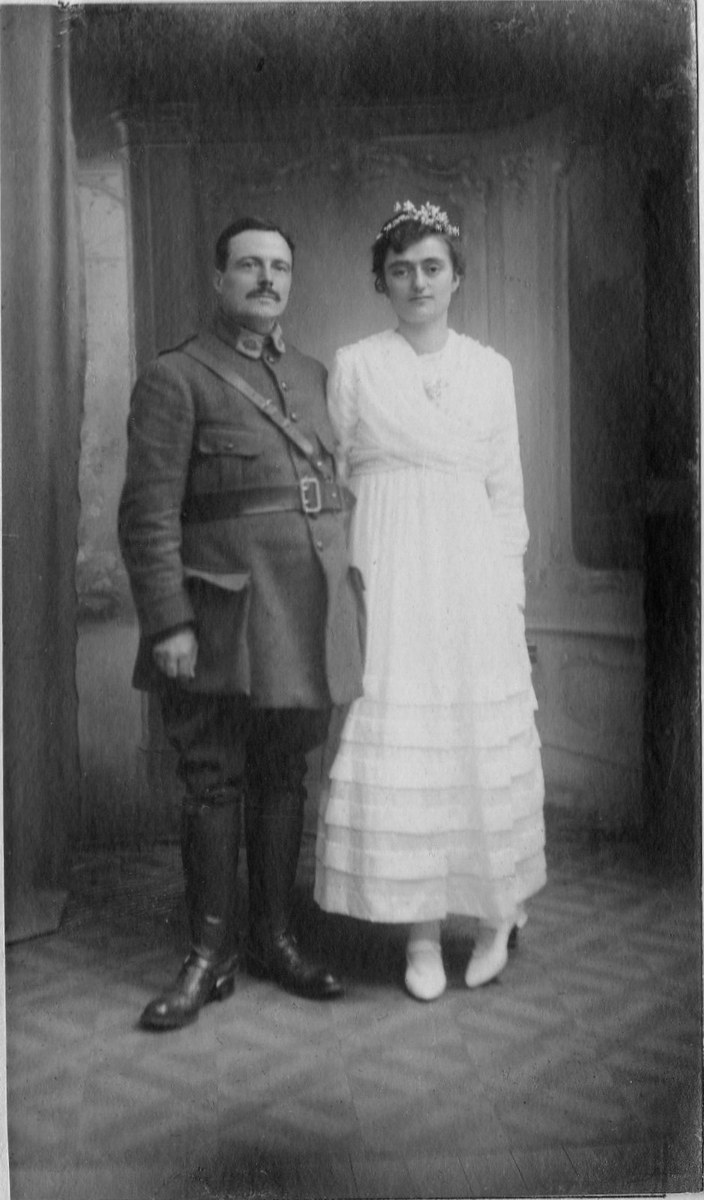
\includegraphics[height=42mm,keepaspectratio]{illustrations/mariage_millau_1917.jpg}
    \par\vspace{1mm}{\scriptsize\textit{Fig. 3.} Mariage d'Hippolyte et Marguerite à Millau (25 octobre 1917).}
  \end{minipage}\hfill
  \begin{minipage}[b]{0.46\textwidth}
    \centering
    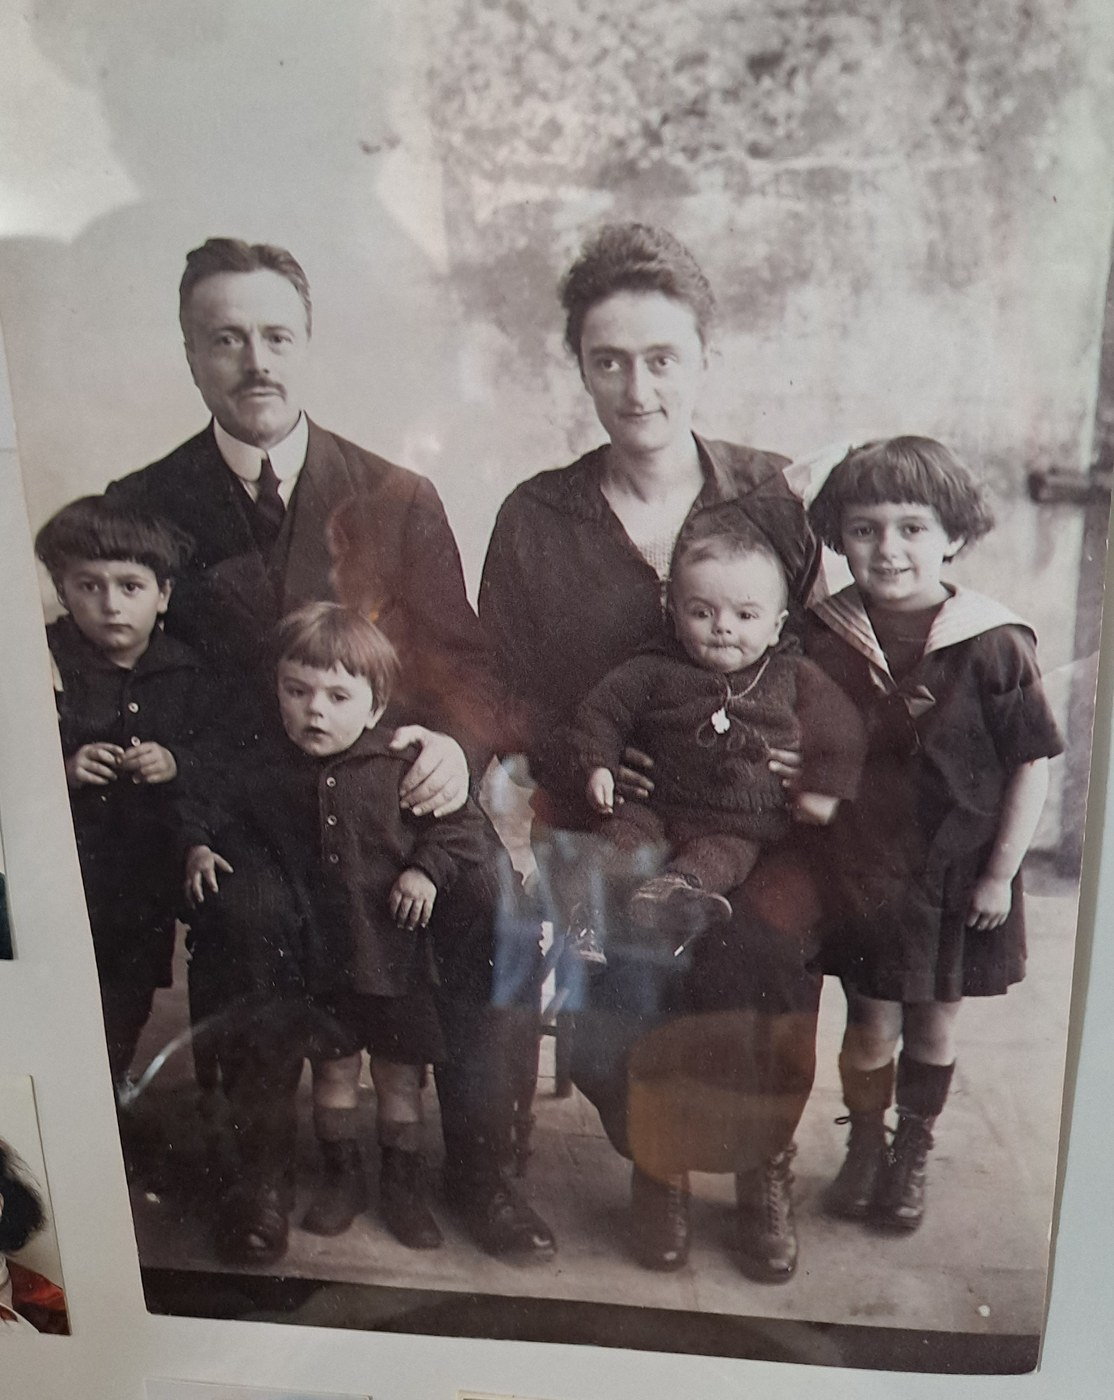
\includegraphics[height=42mm,keepaspectratio]{illustrations/famille_combes_1925.jpg}
    \par\vspace{1mm}{\scriptsize\textit{Fig. 4.} Hippolyte et Marguerite Combes entourés de leurs enfants (vers 1925).}
  \end{minipage}
\end{figure}

{\raggedright\noindent D'après le registre matricule du recrutement de Toulouse (conservé dans le sous-répertoire \texttt{\footnotesize archives\_\allowbreak militaires/\allowbreak fiche\_\allowbreak et\_\allowbreak parcours/}, image \texttt{\footnotesize Fiche\_\allowbreak militaire\_\allowbreak Combes\_\allowbreak Hippolyte.jpg}, accompagnée d'une transcription dérivée) et les actes d'état civil (\texttt{\footnotesize biographie\_\allowbreak et\_\allowbreak famille/\allowbreak etat\_\allowbreak civil\_\allowbreak et\_\allowbreak actes/}) :\par}
\begin{itemize}
  \item \textbf{État civil :} \textbf{Marie Lucien Hippolyte Combes}, né le \textbf{14 août 1876} à \textbf{Millau} (Aveyron), rue des Barris (inscrit sous la date du 22 août 1876 sur la fiche matricule), et décédé le \textbf{2 septembre 1970} à l'\textbf{Hôtel du Centre} à \textbf{Saint-Chély-d'Apcher} (Lozère ; date et commune dans \texttt{Combes-3-part 2.DOC}, établissement transmis par la tradition familiale directe ; inhumé à Millau), fils de \textbf{François Augustin Hippolyte Combes} et de \textbf{Marie Anaïs Alric}, domiciliés à Toulouse (47 rue du Taur). Signalement sur l'image de la fiche : cheveux et sourcils bruns, yeux châtains, taille 1,66 m. Profession portée à l'état civil de la fiche : étudiant en droit ; ultérieurement professeur d'anglais au collège de Nogent-le-Rotrou (Eure-et-Loir) puis au lycée Ingres de Montauban.
  \item \textbf{Parcours militaire et campagnes (1914–1919) :}
    \begin{itemize}
      \item Exempté après deux ans d'ajournement pour « faiblesse générale » (numéro de tirage 74, canton de Toulouse-Nord) ; classé \textbf{Service armé} par le conseil de révision d'Eure-et-Loir le \textbf{18 décembre 1914}.
      \item Appelé à l'activité le \textbf{20 mars 1915} ; arrivé au corps le \textbf{21 mars 1915} au \textbf{10\textsuperscript{e} Régiment d'Artillerie à pied} (39\textsuperscript{e} batterie) à Toulon (campagne simple à l'intérieur du 21 mars au 3 mai 1915).
      \item Détaché à la \textbf{Mission militaire française attachée à l'Armée britannique} aux armées (campagne double) du \textbf{4 mai 1915 au 11 novembre 1918} ; passé administrativement au \textbf{19\textsuperscript{e} Escadron du Train des Équipages Militaires} le \textbf{15 octobre 1915}.
      \item Affecté auprès de la Mission française de Saint-Omer, de la 18\textsuperscript{e} Division britannique (Flesselles, juillet 1915) puis, dès août 1915, d'une compagnie d'\textit{Army Service Corps} de la 18\textsuperscript{e} Division (numéro non donné par la lettre du 21 février 1916), puis des services d'approvisionnement (\textit{Foraging} / \textit{Army Purchase Board}), sans rattachement de corps établi par le petit numéro réservé de la vue \#094.
      \item Affecté le \textbf{24 novembre 1918} à l'\textbf{École militaire préparatoire des Andelys} comme professeur d'anglais ; nommé \textbf{caporal} le \textbf{4 décembre 1918}.
      \item Mis en congé illimité de démobilisation le \textbf{7 février 1919} (se retire à Nogent-le-Rotrou, 17 rue Saint-Hilaire). La rubrique des domiciles porte le \textbf{24 janvier 1920} à Montauban et indique la profession de professeur au lycée Ingres ; cette date ne prouve pas celle de la nomination.
    \end{itemize}
\end{itemize}

\section{Table de concordance intégrale des 186 clichés numériques}

Tous les clichés originaux sont disponibles en double résolution à la racine du dépôt :
\begin{enumerate}
  \item \texttt{scans\_haute\_qualite/} : 186 fichiers JPEG haute résolution (1,03 Go au total, env. 5,9 Mo par scan) ;
  \item \texttt{scans\_compresses/} : 186 fichiers JPEG allégés pour la consultation et l'édition électronique (31,1 Mo au total).
\end{enumerate}

{\fontsize{6pt}{7pt}\selectfont
\renewcommand{\arraystretch}{1.10}
\setlength{\tabcolsep}{2.2pt}
\noindent\begin{longtable}{@{}>{\raggedright\arraybackslash}p{7.5mm}>{\raggedright\arraybackslash}p{24.5mm}>{\raggedright\arraybackslash}p{16.5mm}>{\raggedright\arraybackslash}p{24.5mm}>{\raggedright\arraybackslash}p{52mm}@{}}
\toprule
\textbf{Scan} & \textbf{Fichier JPEG} & \textbf{Vue} & \textbf{Date} & \textbf{Lieu \& Intitulé analytique} \\
\midrule
\endfirsthead
\toprule
\textbf{Scan} & \textbf{Fichier JPEG} & \textbf{Vue} & \textbf{Date} & \textbf{Lieu \& Intitulé analytique (suite)} \\
\midrule
\endhead
\bottomrule
\endfoot
\#001 & \texttt{20251126\_092853.jpg} & Couverture extérieure & 25 juillet 1916 – 30 avril 1917 & \textbf{Somme, Flandres, Artois, Paris, Toulouse, Millau} — PREMIÈRE DE COUVERTURE (Couverture rouge à motif losangé et étiquette bleue rectangulaire : Livre-Journal, 25 juillet 1916 – 30 avril 1917) \\
\#002 & \texttt{20251126\_092932.jpg} & Vue 002 & Mardi 25 juillet 1916 & \textbf{Village lu Sercus [?] ; cantonnement non nommé sur cette vue} — Mardi 25 juillet 1916 — rassemblement avec Curtis, visite de l’église et arrivée de 36 officiers \\
\#003 & \texttt{20251126\_093018.jpg} & Vue 003 & Mercredi 26 juillet 1916 & \textbf{Cantonnement non nommé sur la vue ; Lynde proposé par rapprochement avec le 28 juillet} — Mercredi 26 juillet 1916 — recherche de 36 chambres et annonce du départ \\
\#004 & \texttt{20251126\_093100.jpg} & Vue 004 & Jeudi 27 juillet 1916 & \textbf{Renescure et Hazebrouck (déplacements explicitement nommés)} — Jeudi 27 juillet 1916 — Renescure, Hazebrouck et comptes d’achats \\
\#005 & \texttt{20251126\_093141.jpg} & Vue 005 & Vendredi 28 juillet 1916 & \textbf{De Lynde vers Saint-Jans-Cappel par Hazebrouck (Nord)} — Vendredi 28 juillet 1916 — départ de Lynde, convoi par Hazebrouck et logement au grenier \\
\#006 & \texttt{20251126\_093204.jpg} & Vue 006 & Samedi 29 juillet 1916 & \textbf{Saint-Jans-Cappel et le Mont-Noir (Nord)} — Samedi 29 juillet 1916 — Tournée avec le lieutenant Curtis à Saint-Jans-Cappel et achat de fourrages au Mont-Noir \\
\#007 & \texttt{20251126\_093219.jpg} & Vue 007 & Dimanche 30 et lundi 31 juillet 1916 & \textbf{Saint-Jans-Cappel et Bailleul (Nord)} — Messe dominicale à Saint-Jans-Cappel et corvée de fourrage vert vers Bailleul \\
\#008 & \texttt{20251126\_093240.jpg} & Vue 008 & Mardi 1er août 1916 & \textbf{Saint-Jans-Cappel et Bailleul (Nord)} — Première promenade à Bailleul : la Grand-Place et le beffroi \\
\#009 & \texttt{20251126\_093301.jpg} & Vue 009 & Mercredi 2 et jeudi 3 août 1916 & \textbf{Bailleul (Nord)} — Mercredi 2 et jeudi 3 août 1916 — Promenades dans Bailleul, maisons flamandes et dentellières au fuseau \\
\#010 & \texttt{20251126\_093316.jpg} & Vue 010 & Vendredi 4 août 1916 (matin et après-midi) & \textbf{Saint-Jans-Cappel, Bailleul, Steenwerck, La Croix-du-Bac (Nord)} — Chevauchée à La Croix-du-Bac par Steenwerck et repos dans le « garret » \\
\#011 & \texttt{20251126\_093332.jpg} & Vue 011 & Vendredi 4 août 1916 (soir) & \textbf{Saint-Jans-Cappel (Nord)} — Soirée solitaire à la ferme et prière du soir de la famille flamande \\
\#012 & \texttt{20251126\_093347.jpg} & Vue 012 & Samedi 5 août 1916 & \textbf{De Saint-Jans-Cappel à La Croix-du-Bac / Steenwerck (Nord)} — Départ du convoi avec les A.S.C. men et étape à La Croix-du-Bac \\
\#013 & \texttt{20251126\_093412.jpg} & Vue 013 & Dimanche 6 août 1916 & \textbf{La Croix-du-Bac et Bac-Saint-Maur (Nord)} — Dimanche 6 août 1916 — Au refilling point sur les bords de la Lys avec le lieutenant Curtis, rencontre de Maurin et concert militaire \\
\#014 & \texttt{20251126\_093426.jpg} & Vue 014 & Lundi 7 août 1916 & \textbf{Steenwerck et route de Bac-Saint-Maur (Nord)} — Quête de cantonnements avec le lieutenant Curtis, départ inopiné de la compagnie et nouvelle chambre \\
\#015 & \texttt{20251126\_093455.jpg} & Vue 015 & Mardi 8 et mercredi 9 août 1916 & \textbf{Route de Bac-Saint-Maur, Steenwerck (Nord)} — Deux journées de canicule, de poussière et de moustiques dans la vallée de la Lys \\
\#016 & \texttt{20251126\_093506.jpg} & Vue 016 & Jeudi 10 août 1916 & \textbf{Bac-Saint-Maur et Sailly-sur-la-Lys (Nord / Pas-de-Calais)} — Promenade à Sailly-sur-la-Lys, l'église bombardée et conversation avec l'éclusier sur le général Maxse \\
\#017 & \texttt{20251126\_093529.jpg} & Vue 017 & Vendredi 11 août 1916 & \textbf{Secteur à l’ouest d’Armentières ; position précise de la blanchisserie non établie} — Vendredi 11 août 1916 — bombardement, blanchisserie Barbry et descente à la cave \\
\#018 & \texttt{20251126\_093544.jpg} & Vue 018 & Samedi 12 août 1916 & \textbf{Rives de la Lys, Bac-Saint-Maur (Nord)} — Sieste au bord de la Lys dans un champ de luzerne face aux blés mûrs \\
\#019 & \texttt{20251126\_093618.jpg} & Vue 019 & Dimanche 13 et lundi 14 août 1916 & \textbf{Bac-Saint-Maur et direction d'Armentières (Nord)} — Attente vaine d'une lettre de Marguerite, « pot-au-noir » et orage sur la Lys \\
\#020 & \texttt{20251126\_093746.jpg} & Vue 020 & Mardi 15 août 1916 (Assomption) & \textbf{Bac-Saint-Maur / Steenwerck (Nord)} — Journée pluvieuse du 15 août dans la mansarde et comptes de blanchissage \\
\#021 & \texttt{20251126\_093843.jpg} & Vue 021 & Vendredi 18 et samedi 19 août 1916 & \textbf{Steenwerck, Fleurbaix et secteur d'Armentières (Nord)} — Vendredi 18 et Samedi 19 août 1916 — Giboulées d'août, perception de la solde et chevauchée sous l'orage avec le lieutenant Curtis \\
\#022 & \texttt{20251126\_093857.jpg} & Vue 022 & Samedi 19 août 1916 (suite) & \textbf{Erquinghem-Lys, Fleurbaix et Armentières (Pas-de-Calais / Nord)} — Traversée de Fleurbaix et d'Armentières dévastées par les obus \\
\#023 & \texttt{20251126\_093922.jpg} & Vue 023 & Dimanche 20 et lundi 21 août 1916 & \textbf{Erquinghem-Lys et Steenwerck (Nord)} — Café chez M. Barbry avec les adjudants Lupin et Schumacher et préparatifs de départ \\
\#024 & \texttt{20251126\_093941.jpg} & Vue 024 & Mardi 22 août 1916 & \textbf{Steenwerck, Bac-Saint-Maur et Erquinghem-Lys (Nord)} — Mardi 22 août 1916 — Bière chez un charcutier avec Maurin évoquant les beautés d'Antibes et envoi d’un sac de linge à Nogent \\
\#025 & \texttt{20251126\_093955.jpg} & Vue 025 & Mercredi 23 août 1916 & \textbf{Estaires (Nord)} — Chevauchée jusqu'à Estaires : l'église Saint-Vaast, l'Hôtel de Ville et l'hygiène par l'exercice \\
\#026 & \texttt{20251126\_094019.jpg} & Vue 026 & Jeudi 24 août 1916 & \textbf{Steenwerck (Nord)} — Jeudi 24 août 1916 — Église de Steenwerck, transport des sacs sous la tente de l'office par Fisher et adieux aux Flandres \\
\#027 & \texttt{20251126\_094045.jpg} & Vue 027 & Vendredi 25 août 1916 & \textbf{De Steenwerck et Bailleul à Saint-Pol-sur-Ternoise (Pas-de-Calais)} — Embarquement ferroviaire à Bailleul et descente par Hazebrouck et Lillers vers Saint-Pol-sur-Ternoise \\
\#028 & \texttt{20251126\_094058.jpg} & Vue 028 & Vendredi 25 août 1916 (suite) & \textbf{De Bailleul à Saint-Pol et Marquay (Pas-de-Calais)} — Mélancolie du voyage en train au son de l'harmonica et arrivée nocturne à Marquay \\
\#029 & \texttt{20251126\_094159.jpg} & Vue 029 & Samedi 26 août 1916 & \textbf{Marquay et Bailleul-aux-Cornailles (Pas-de-Calais)} — Samedi 26 août 1916 — promenade à Bailleul-aux-Cornailles et mauvais logement \\
\#030 & \texttt{20251126\_094215.jpg} & Vue 030 & Lundi 28 et mardi 29 août 1916 & \textbf{Marquay (Pas-de-Calais)} — Lundi 28 et Mardi 29 août 1916 — Bourbiers d'Artois, corvées de fourrage avec le lieutenant Curtis et entrée en guerre de la Roumanie \\
\#031 & \texttt{20251126\_094238.jpg} & Vue 031 & Mercredi 30 août 1916 & \textbf{Cantonnement non nommé sur cette vue ; Marquay par continuité des entrées voisines} — Tempête de vent dans les grands arbres du voisinage et fourrage sous les ondées \\
\#032 & \texttt{20251126\_094250.jpg} & Vue 032 & Jeudi 31 août 1916 & \textbf{Marquay, Ramecourt, Saint-Michel, Saint-Pol-sur-Ternoise et Ostreville (Pas-de-Calais)} — Saint-Pol : promenade, église et achats \\
\#033 & \texttt{20251126\_094310.jpg} & Vue 033 & Vendredi 1er septembre 1916 & \textbf{Marquay et Ligny-Saint-Flochel (Pas-de-Calais)} — Ligny-Saint-Flochel : église, cimetière et attente \\
\#034 & \texttt{20251126\_094324.jpg} & Vue 034 & Samedi 2 et dimanche 3 septembre 1916 & \textbf{Marquay et Saint-Pol-sur-Ternoise (Pas-de-Calais)} — Promenades à Saint-Pol sous un ciel menaçant \\
\#035 & \texttt{20251126\_094345.jpg} & Vue 035 & Lundi 4 et mardi 5 septembre 1916 & \textbf{Marquay et Roëllecourt (Pas-de-Calais)} — Roellecourt et départ retardé \\
\#036 & \texttt{20251126\_094449.jpg} & Vue 036 & Dimanche 3 (addition) / mardi 5 septembre 1916 & \textbf{Marquay et Saint-Pol-sur-Ternoise (Pas-de-Calais)} — Avoines et achats à Saint-Pol \\
\#037 & \texttt{20251126\_094511.jpg} & Vue 037 & Mercredi 6 et jeudi 7 septembre 1916 & \textbf{Marquay, Bailleul-aux-Cornailles, Saint-Pol et Saint-Michel-sur-Ternoise (Pas-de-Calais)} — Repos au grand air et promenades vers Saint-Pol \\
\#038 & \texttt{20251126\_094524.jpg} & Vue 038 & Vendredi 8 septembre 1916 & \textbf{Marquay et ferme de Ryonval (Pas-de-Calais)} — Wagons des Bedfords et promenade nocturne \\
\#039 & \texttt{20251126\_094545.jpg} & Vue 039 & Samedi 9 septembre 1916 & \textbf{De Marquay et Ligny-Saint-Flochel à Monts-en-Ternois (Pas-de-Calais)} — De Marquay à Monts-en-Ternois \\
\#040 & \texttt{20251126\_094600.jpg} & Vue 040 & Dimanche 10 septembre 1916 & \textbf{De Monts-en-Ternois à Oppy et Beaudricourt (Pas-de-Calais)} — Étape à Oppy et service à Beaudricourt \\
\#041 & \texttt{20251126\_094621.jpg} & Vue 041 & Lundi 11 septembre 1916 & \textbf{D'Oppy (Beaudricourt) à Lucheux, Thièvres et Raincheval (Pas-de-Calais / Somme)} — Chevauchée vers Raincheval par Lucheux \\
\#042 & \texttt{20251126\_094639.jpg} & Vue 042 & Mardi 12 et mercredi 13 septembre 1916 & \textbf{Raincheval (Somme)} — Invitation permanente au mess et forêt \\
\#043 & \texttt{20251126\_094654.jpg} & Vue 043 & Jeudi 14 et vendredi 15 septembre 1916 & \textbf{Raincheval et Acheux-en-Amiénois (Somme)} — Acheux et exercices à Raincheval \\
\#044 & \texttt{20251126\_094706.jpg} & Vue 044 & Dimanche 17 septembre 1916 & \textbf{Raincheval (Somme)} — Bois, fourrage et collection de faïences \\
\#045 & \texttt{20251126\_094726.jpg} & Vue 045 & Lundi 18 septembre 1916 & \textbf{Raincheval, Hédauville, Forceville et Acheux-en-Amiénois (Somme)} — Mission française et retour sous la pluie \\
\#046 & \texttt{20251126\_094738.jpg} & Vue 046 & Jeudi 21 septembre 1916 & \textbf{Raincheval et Acheux-en-Amiénois (Somme)} — Accalmie et perception de la solde \\
\#047 & \texttt{20251126\_094822.jpg} & Vue 047 & Vendredi 22 septembre 1916 & \textbf{Raincheval (Somme)} — Football et annonce d’un déplacement \\
\#048 & \texttt{20251126\_094835.jpg} & Vue 048 & Samedi 23 septembre 1916 & \textbf{Raincheval, Léalvillers, Acheux et Forceville (Somme)} — Message de Pizzi et bivouac \\
\#049 & \texttt{20251126\_103003.jpg} & Vue 049 & Dimanche 24 septembre 1916 & \textbf{Forceville et Acheux-en-Amiénois (Somme)} — Hutte et préparation du départ \\
\#050 & \texttt{20251126\_103019.jpg} & Vue 050 & Lundi 25 septembre 1916 (matin et après-midi) & \textbf{Forceville et gare d'Acheux-Varennes (Somme)} — Forceville et départ par Acheux-Varennes \\
\#051 & \texttt{20251126\_103036.jpg} & Vue 051 & Lundi 25 septembre 1916 (soir et nuit) & \textbf{Gézaincourt, Amiens, Longueau et train vers Paris} — Gézaincourt, Amiens et bombardement nocturne \\
\#052 & \texttt{20251126\_103109.jpg} & Vue 052 & Mardi 26 septembre 1916 (matin et après-midi) & \textbf{Le Bourget et Paris (Gare du Nord, Tuileries, Orsay, Invalides, rive gauche)} — Du Bourget à Paris : démarches et courses \\
\#053 & \texttt{20251126\_103131.jpg} & Vue 053 & Mardi 26 septembre 1916 (après-midi et soir) & \textbf{Paris (Tour Saint-Jacques, rue de Rivoli, librairie Colin, gare d'Orsay)} — Paris : promenade, livres et dépenses \\
\#054 & \texttt{20251126\_103146.jpg} & Vue 054 & Mercredi 27 septembre 1916 & \textbf{Toulouse (Sainte-Marie-des-Champs)} — Arrivée à Toulouse et retrouvailles \\
\#055 & \texttt{20251126\_103215.jpg} & Vue 055 & Jeudi 28 septembre 1916 & \textbf{Toulouse (Sainte-Marie, barrière Saint-Agne, Pouvourville, Pech-David)} — Souvenirs et promenade vers Pech-David \\
\#056 & \texttt{20251126\_103227.jpg} & Vue 056 & Vendredi 29 septembre 1916 & \textbf{Toulouse, Purpan, Blagnac et les Ponts-Jumeaux (Haute-Garonne)} — Blagnac et achat d’un sautoir \\
\#057 & \texttt{20251126\_103247.jpg} & Vue 057 & Samedi 30 septembre 1916 & \textbf{Toulouse (Sainte-Marie, Montaudran et cimetière de Terre-Cabade)} — Montaudran et serments à Terre-Cabade \\
\#058 & \texttt{20251126\_103301.jpg} & Vue 058 & Dimanche 1er octobre 1916 & \textbf{Toulouse (Cathédrale Saint-Étienne, Sainte-Marie et Lardenne)} — Saint-Étienne, Lardenne et le Touch \\
\#059 & \texttt{20251126\_103321.jpg} & Vue 059 & Lundi 2 octobre 1916 & \textbf{Toulouse (Appartement, Sainte-Marie, chapelle de Nazareth, rue d'Alsace-Lorraine)} — Souvenirs et visite de Marguerite \\
\#060 & \texttt{20251126\_103335.jpg} & Vue 060 & Mardi 3 octobre 1916 & \textbf{Toulouse (Cathédrale Saint-Étienne, rue d'Alsace-Lorraine, marché Victor-Hugo, route de Castanet)} — Saint-Étienne et présentation de la fiancée \\
\#061 & \texttt{20251126\_103455.jpg} & Vue 061 & Mardi 3 octobre 1916 (suite) & \textbf{Toulouse} — Paiements à Guiraud et à Guilhem, visite à Mme de Labarthe \\
\#062 & \texttt{20251126\_103514.jpg} & Vue 062 & Mercredi 4 octobre 1916 & \textbf{Toulouse (Sainte-Marie et gare Matabiau)} — Préparatifs et séparation à la gare \\
\#063 & \texttt{20251126\_103538.jpg} & Vue 063 & Jeudi 5 octobre 1916 & \textbf{Paris (Gare d'Orsay, Gare du Nord, église Saint-Vincent-de-Paul, Grands Magasins du Louvre)} — Traversée de Paris sous la pluie : l'église Saint-Vincent-de-Paul et les salons du Louvre \\
\#064 & \texttt{20251126\_103554.jpg} & Vue 064 & Mercredi 4 octobre 1916 (soir et nuit) & \textbf{Gare de Toulouse et train de nuit Toulouse – Paris-Orsay} — Fin des adieux en gare de Toulouse, nuit blanche dans l'express d'Orsay et comptes de départ \\
\#065 & \texttt{20251126\_103743.jpg} & Vue 065 & Jeudi 5 octobre 1916 (après-midi et soir) & \textbf{Paris (Gare du Nord), Amiens et Doullens (Somme)} — Train de l’après-midi de Paris-Nord à Amiens et arrivée à minuit en gare de Doullens \\
\#066 & \texttt{20251126\_103755.jpg} & Vue 066 & Vendredi 6 octobre 1916 (matin et midi) & \textbf{Doullens, Canaples et Barlette (Somme)} — Vendredi 6 octobre 1916 — Fin de la nuit à la gare de Doullens, train de 7 h 25 et retour en lorry de la 54e Brigade auprès de la 152nd Coy A.S.C. \\
\#067 & \texttt{20251126\_103816.jpg} & Vue 067 & Vendredi 6 octobre 1916 (après-midi et soir) & \textbf{Hameau de Barlette (Ribeaucourt) et Bernaville (Somme)} — Installation au hameau de Barlette (Ribeaucourt) et visa de permission à Bernaville \\
\#068 & \texttt{20251126\_103828.jpg} & Vue 068 & Samedi 7 octobre 1916 & \textbf{Hameau de Barlette, Ribeaucourt (Somme)} — Tempête nocturne sur les vergers de Barlette et règlement des frais de mess au capitaine Panton \\
\#069 & \texttt{20251126\_103845.jpg} & Vue 069 & Dimanche 8 octobre 1916 & \textbf{Barlette (Ribeaucourt) et Bernaville (Somme)} — Dimanche de repos à Barlette et perception de la solde à pied à Bernaville sous la rafale \\
\#070 & \texttt{20251126\_103857.jpg} & Vue 070 & Lundi 9 octobre 1916 & \textbf{Barlette et forêt de Ribeaucourt (Somme)} — Promenade forestière et clair de lune d’octobre \\
\#071 & \texttt{20251126\_103913.jpg} & Vue 071 & Mardi 10 octobre 1916 & \textbf{Barlette et bois de Ribeaucourt (Somme)} — Corvée de fourrage vert en lisière des bois aux couleurs d'automne et nuit de pleine lune \\
\#072 & \texttt{20251126\_103948.jpg} & Vue 072 & Mercredi 11 octobre 1916 & \textbf{Barlette et Ribeaucourt (Somme)} — Convoi de luzerne sous une pluie battante derrière le grand bois de Ribeaucourt \\
\#073 & \texttt{20251126\_104011.jpg} & Vue 073 & Jeudi 12 et vendredi 13 octobre 1916 & \textbf{Barlette, Ribeaucourt et Prouville (Somme)} — Fourrage, symphonie du vent dans les bois et course à cheval à Prouville \\
\#074 & \texttt{20251126\_104027.jpg} & Vue 074 & Dimanche 15 octobre 1916 & \textbf{De Barlette (Ribeaucourt) à Beauval (Somme)} — Départ définitif de Barlette sous les averses et arrivée de la colonne à Beauval \\
\#075 & \texttt{20251126\_104057.jpg} & Vue 075 & 16 octobre 1916 & \textbf{Beauval, Beauquesne, Puchevillers, Warloy-Baillon (Somme)} — Départ de Beauval sous un air glacial et marche vers Warloy-Baillon \\
\#076 & \texttt{20251126\_104118.jpg} & Vue 076 & 16 (comptes) – 17 octobre 1916 (matin) & \textbf{Beauval, Warloy-Baillon (Somme)} — Nuit glaciale sous la tente à Warloy-Baillon et départ de la colonne \\
\#077 & \texttt{20251126\_104143.jpg} & Vue 077 & 17 octobre 1916 (suite) & \textbf{Senlis-le-Sec, Bouzincourt, Hédauville (Somme)} — Bivouac dans un champ dévasté entre Bouzincourt et Hédauville \\
\#078 & \texttt{20251126\_104157.jpg} & Vue 078 & 18 octobre 1916 & \textbf{Camp de Bouzincourt, Albert (Somme)} — Visite d'Albert bombardée et de sa basilique en ruines \\
\#079 & \texttt{20251126\_104222.jpg} & Vue 079 & 18 octobre 1916 (suite) & \textbf{Camp de Bouzincourt, Albert (Somme)} — Convois, soirée dans la mess-tent et compte à la mission d’Albert \\
\#080 & \texttt{20251126\_104235.jpg} & Vue 080 & 19 octobre 1916 & \textbf{Camp de Bouzincourt, Albert (Brickfield Area, Somme)} — Pluie torrentielle et installation au Brickfield Area d'Albert \\
\#081 & \texttt{20251126\_104314.jpg} & Vue 081 & 20 octobre 1916 & \textbf{Albert (Brickfield Area, Somme)} — Duel d'artillerie formidable et horizon embrasé au-dessus d'Albert \\
\#082 & \texttt{20251126\_104331.jpg} & Vue 082 & 21 octobre 1916 & \textbf{Albert, Aveluy (Somme)} — Gelée d'octobre, reconnaissance vers Aveluy et veillée près du poêle \\
\#083 & \texttt{20251126\_104346.jpg} & Vue 083 & 22 octobre 1916 & \textbf{Albert (Somme)} — La « Vierge penchée » d'Albert et la rumeur de rappel des jeunes R.A.T. \\
\#084 & \texttt{20251126\_104400.jpg} & Vue 084 & 23 octobre 1916 & \textbf{Albert, La Boisselle (Somme)} — Visite des abris souterrains allemands et du grand cratère de La Boisselle \\
\#085 & \texttt{20251126\_104418.jpg} & Vue 085 & 24 – 25 octobre 1916 & \textbf{Albert (Somme)} — Maintien confirmé à la Mission française et averses dans les fondrières d'Albert \\
\#086 & \texttt{20251126\_104440.jpg} & Vue 086 & 26 – 28 octobre 1916 & \textbf{Albert (Somme)} — Journées de pluie, d'inaction et d'accalmie dans Albert dévastée \\
\#087 & \texttt{20251126\_104459.jpg} & Vue 087 & 29 – 30 octobre 1916 & \textbf{Albert, Acheux, Senlis-le-Sec (Somme)} — Enquête sur les pailles à Acheux, rencontre d'un artilleur belge et tempête \\
\#088 & \texttt{20251126\_104515.jpg} & Vue 088 & 31 octobre 1916 & \textbf{Albert (Somme)} — Éclaircie de fin octobre et bombardement d'Albert \\
\#089 & \texttt{20251126\_104547.jpg} & Vue 089 & 1er novembre 1916 & \textbf{Albert (Somme)} — Toussaint au cimetière d’Albert, prise d’armes et ordre de départ \\
\#090 & \texttt{20251126\_104601.jpg} & Vue 090 & 2 novembre 1916 & \textbf{Albert, Acheux-en-Amiénois (Somme)} — Ordre écrit au Train Office et départ sous la pluie vers Acheux \\
\#091 & \texttt{20251126\_104623.jpg} & Vue 091 & 2 (soir) – 3 novembre 1916 & \textbf{Acheux, Raincheval, Albert (Somme)} — Course nocturne à Raincheval et aller-retour au camp d’Albert \\
\#092 & \texttt{20251126\_104636.jpg} & Vue 092 & 4 novembre 1916 & \textbf{Acheux, Bertrancourt, Bus-lès-Artois, Albert (Somme)} — Course à pied à Bertrancourt et retrouvailles avec l'interprète Cordonnier \\
\#093 & \texttt{20251126\_104647.jpg} & Vue 093 & 2 (soir) – 3 novembre 1916 [cliché bis] & \textbf{Acheux, Raincheval, Albert (Somme)} — Second cliché archivistique du feuillet des 2–3 novembre 1916 (doublon de numérisation) \\
\#094 & \texttt{20251126\_104702.jpg} & Vue 094 & 5 novembre 1916 & \textbf{Acheux-en-Amiénois (Somme)} — Emménagement au n° 1 route de Léalvillers et convocation chez le capitaine Huguet \\
\#095 & \texttt{20251126\_104714.jpg} & Vue 095 & 6 – 7 novembre 1916 & \textbf{Acheux, Arquèves (Belle-Église), Hérissart, Rubempré, Coisy (Somme)} — Courses à Belle-Église et Coisy, nostalgie de la 152e Compagnie et convois vers la ligne de feu \\
\#096 & \texttt{20251126\_104728.jpg} & Vue 096 & 8 – 9 novembre 1916 & \textbf{Acheux, Forceville, Varennes, Warloy, Senlis-le-Sec, Albert (Somme)} — Promenades en auto à Forceville, Varennes et thé au mess de la 152e Compagnie à Albert \\
\#097 & \texttt{20251126\_104739.jpg} & Vue 097 & 10 – 11 novembre 1916 & \textbf{Acheux, Raincheval, Léalvillers, Varennes (Somme)} — Courses à Raincheval et Varennes, rencontre d’un interprète et bombardement d’Acheux \\
\#098 & \texttt{20251126\_104801.jpg} & Vue 098 & 12 – 14 novembre 1916 & \textbf{Acheux, Varennes, Contay, Beauquesne, Raincheval, Doullens, Frévent (Somme / Pas-de-Calais)} — Bataille de Beaumont-Hamel (13–14 novembre), convois de blessés et foire de Doullens \\
\#099 & \texttt{20251126\_104814.jpg} & Vue 099 & 15 – 16 novembre 1916 & \textbf{Acheux, Albert, Raincheval, Louvencourt, Toutencourt, Hérissart (Somme)} — Canonnade vers Beaumont-sur-Ancre et rencontre à Hérissart \\
\#100 & \texttt{20251126\_104831.jpg} & Vue 100 & 17 – 18 novembre 1916 & \textbf{Acheux, Authie, Orville, Amplier, Albert (Somme / Pas-de-Calais)} — Premières fortes gelées, conférence sur la Russie au Y.M.C.A. et première neige \\
\#101 & \texttt{20251126\_104849.jpg} & Vue 101 & 20 – 21 novembre 1916 & \textbf{Acheux, Bouzincourt, Contay [?], Englebelmer, Léalvillers (Somme)} — Défilé de troupes et de prisonniers allemands à Acheux, nuit à Englebelmer et friction avec Curtis \\
\#102 & \texttt{20251126\_104903.jpg} & Vue 102 & 22 – 23 novembre 1916 & \textbf{Acheux, Amplier, Authieule, Authie (Somme / Pas-de-Calais)} — Indisposition nocturne, travaux de couture et tournée à Amplier et Authie \\
\#103 & \texttt{20251126\_104916.jpg} & Vue 103 & 25 – 26 novembre 1916 & \textbf{Acheux, Hérissart (Somme)} — Bombardement du côté de la sucrerie d’Acheux et visite de M. Deloney \\
\#104 & \texttt{20251126\_104932.jpg} & Vue 104 & 28 – 30 novembre 1916 & \textbf{Acheux, Martinsart, Raincheval, Puchevillers, Rubempré, Septenville, Pierregot, Hérissart (Somme)} — Thé au château de Martinsart et brouillard sur la campagne \\
\#105 & \texttt{20251126\_104946.jpg} & Vue 105 & 1er – 2 décembre 1916 & \textbf{Acheux, Franvillers, Buire-sur-l'Ancre, Ribemont, Heilly, Toutencourt (Somme)} — Tournée à Franvillers et Buire-sur-l'Ancre, arrivée imprévue du très jeune capitaine Williams \\
\#106 & \texttt{20251126\_105005.jpg} & Vue 106 & 3 – 4 décembre 1916 & \textbf{Acheux, Septenville, Hérissart, Corbie, Villers-Bretonneux, Marcelcave, Warfusée-Abancourt, Arquèves, Louvencourt (Somme)} — Longue randonnée jusqu'à Corbie, Villers-Bretonneux et Marcelcave dans la brume glaciale \\
\#107 & \texttt{20251126\_105017.jpg} & Vue 107 & 5 – 6 décembre 1916 & \textbf{Acheux, Authie, Bayencourt, Coigneux, Louvencourt, Raincheval (Somme / Pas-de-Calais)} — Course jusqu'aux ruines de Bayencourt et Coigneux, départ de Curtis et confidences de Williams \\
\#108 & \texttt{20251126\_105046.jpg} & Vue 108 & 7 – 8 décembre 1916 & \textbf{Acheux, Arquèves (Belle-Église), Hédauville, Englebelmer, Saint-Léger-lès-Authie (Somme)} — Les enfants de la fermière belge de Belle-Église et le village désert d'Englebelmer \\
\#109 & \texttt{20251126\_105057.jpg} & Vue 109 & 9 – 11 décembre 1916 & \textbf{Acheux, Authie, Orville, Saulty, L’Arbret (Somme / Pas-de-Calais); Belle-Église biffé} — Randonnée pluvieuse jusqu’à Saulty et L’Arbret; jugement sur Williams et indisposition \\
\#110 & \texttt{20251126\_105112.jpg} & Vue 110 & 12 – 14 décembre 1916 & \textbf{Acheux, Senlis-le-Sec, Toutencourt, Belle-Église, Puchevillers, Harponville (Somme)} — Paysage de neige aux fenêtres d'Acheux et réunion des réfugiés d'Englebelmer à Toutencourt \\
\#111 & \texttt{20251126\_105125.jpg} & Vue 111 & 15 – 18 décembre 1916 & \textbf{Acheux, Belle-Église, Arquèves, Raincheval, Toutencourt, Ferme du Quesnoy (Somme)} — Cahots sur les routes défoncées et portrait critique du jeune capitaine Williams \\
\#112 & \texttt{20251126\_105142.jpg} & Vue 112 & 22 – 24 décembre 1916 & \textbf{Acheux, Senlis-le-Sec, Rubempré, Quesnoy (identification non établie), Léalvillers, Saint-Léger, Orville, Authie, Toutencourt, Puchevillers, Louvencourt} — Crise épistolaire avec Marguerite (« velléités de rupture ») et l'incident du « Bloody France ! » \\
\#113 & \texttt{20251126\_105155.jpg} & Vue 113 & 19 – 20 décembre 1916 & \textbf{Acheux, Belle-Église, Raincheval, Quesnoy (identification non établie), Beauquesne} — Attente devant l’Army P. Board à Raincheval et grandes gelées d’avant Noël \\
\#114 & \texttt{20251126\_105239.jpg} & Vue 114 & 25 décembre 1916 & \textbf{Acheux-en-Amiénois (Somme)} — Noël 1916 à Acheux : insomnie, perplexité morale et concert au Y.M.C.A. \\
\#115 & \texttt{20251126\_105252.jpg} & Vue 115 & 26 – 27 décembre 1916 & \textbf{Acheux, Raincheval, Arquèves, Beauquesne, Quesnoy (identification non établie), Doullens} — Location d'une machine à battre chez Mme Capron à Beauquesne et course rapide à Doullens \\
\#116 & \texttt{20251126\_105400.jpg} & Vue 116 & 28 – 29 décembre 1916 & \textbf{Acheux, Léalvillers, Raincheval, Quesnoy (identification non établie), Louvencourt} — Concert des « 13th Corps Archie Singers » et tournée dans la voiture Sunbeam du major Levy \\
\#117 & \texttt{20251126\_105411.jpg} & Vue 117 & 30 – 31 décembre 1916 & \textbf{Acheux, Franvillers, Senlis-le-Sec, Belle-Église, Raincheval, Beauquesne (Somme)} — Nouvel éclat et excuses contrites du capitaine Williams à la Saint-Sylvestre \\
\#118 & \texttt{20251126\_105428.jpg} & Vue 118 & 1er – 2 janvier 1917 & \textbf{Acheux, Toutencourt, Saulty, Louvencourt, Raincheval (Somme / Pas-de-Calais)} — Jour de l'An 1917 à Acheux, tournées à Toutencourt, Saulty et Louvencourt \\
\#119 & \texttt{20251126\_105446.jpg} & Vue 119 & 3 janvier 1917 & \textbf{Acheux, Belle-Église, Montigny, Amiens (Somme)} — Course à Amiens : l'Hôtel de la Paix, le capitaine Trefcon et la cathédrale \\
\#120 & \texttt{20251126\_105848.jpg} & Vue 120 & 4 – 5 janvier 1917 & \textbf{Acheux, Septenville, Beauquesne (Somme)} — Concert à la Y.M.C.A. et contrat avec Mme Capron à Beauquesne \\
\#121 & \texttt{20251126\_105908.jpg} & Vue 121 & 6 – 9 janvier 1917 & \textbf{Acheux, Louvencourt, Bertrancourt, Authie, Arquèves, Raincheval, Saint-Léger, Hédauville (Somme)} — Déplacements de troupes autour d'Acheux et visite à la 150e Compagnie à Hédauville \\
\#122 & \texttt{20251126\_105920.jpg} & Vue 122 & 10 – 12 janvier 1917 & \textbf{Acheux, Saint-Léger, Belle-Église, Authie, Arquèves, Louvencourt, Raincheval, Beauquesne, Septenville, Rubempré (Somme)} — Canonnade sur Miraumont, retrouvailles avec Morris et tempête de grésil sur les plateaux \\
\#123 & \texttt{20251126\_105931.jpg} & Vue 123 & 13 – 15 janvier 1917 & \textbf{Acheux, Beaucourt, Montigny, Louvencourt, Saint-Léger, Beauquesne, Raincheval, Doullens (Somme)} — Départ fixé au 26 janvier, arbres ouatés de neige et course à Doullens \\
\#124 & \texttt{20251126\_105945.jpg} & Vue 124 & 16 – 17 janvier 1917 & \textbf{Acheux, Bouzincourt, Senlis-le-Sec, Rubempré, Hérissart, Toutencourt, Doullens, Auxi-le-Château (Somme / Pas-de-Calais)} — Étendues blanches d'Hérissart et visite à Auxi-le-Château chez le collectionneur M. Renard \\
\#125 & \texttt{20251126\_105956.jpg} & Vue 125 & 18 – 19 janvier 1917 & \textbf{Acheux, Belle-Église, Raincheval, Puchevillers (Somme)} — Plaines blanches confondues avec le ciel mat et neige cristallisée à Puchevillers \\
\#126 & \texttt{20251126\_110011.jpg} & Vue 126 & 20 – 23 janvier 1917 & \textbf{Acheux, Louvencourt (Somme)} — Grand gel sec, retour à pied de Louvencourt et préparatifs de permission \\
\#127 & \texttt{20251126\_110024.jpg} & Vue 127 & 23 (soir) – 25 janvier 1917 & \textbf{Acheux-en-Amiénois (Somme)} — Conférence sur le Canada au Y.M.C.A., eau gelée dans la chambre et fin des préparatifs \\
\#128 & \texttt{20251126\_110048.jpg} & Vue 128 & 26 janvier 1917 & \textbf{Acheux, Gare de Varennes, Gézaincourt (Somme)} — Départ en permission de la gare de Varennes et longue attente nocturne à Gézaincourt \\
\#129 & \texttt{20251126\_110059.jpg} & Vue 129 & 26 janvier 1917 (suite, nuit du 26 au 27) & \textbf{Acheux, Gézaincourt, Amiens (Somme)} — Arrivée à Amiens à deux heures du matin et état de la caisse de voyage \\
\#130 & \texttt{20251126\_110124.jpg} & Vue 130 & 27 janvier 1917 (matin et midi) & \textbf{Amiens, Paris (Gare du Nord, Gare d'Orsay), Neuilly-sur-Seine} — Nuit glaciale à la gare d'Amiens avec l'interprète Boilly et arrivée à Paris et Neuilly \\
\#131 & \texttt{20251126\_110135.jpg} & Vue 131 & 27 janvier 1917 (suite) & \textbf{Neuilly-sur-Seine, Paris (Boulevard Saint-Michel, Hôtel de Ville, Gare d'Orsay)} — Déjeuner à Neuilly chez Mme Faure, visite chez l'opticien Imbert et départ pour Toulouse \\
\#132 & \texttt{20251126\_110149.jpg} & Vue 132 & 27 (comptes) – 28 janvier 1917 (matin) & \textbf{Paris, Toulouse (Gare Matabiau, Saint-Michel, Sainte-Marie)} — Dépenses parisiennes et arrivée matinale à Toulouse : souvenirs des disparus et visite de l'oncle Émile \\
\#133 & \texttt{20251126\_110200.jpg} & Vue 133 & 28 janvier 1917 (suite) & \textbf{Toulouse (Quartier Sainte-Marie / Côte Pavée)} — Retrouvailles infiniment tendres avec Marguerite à Sainte-Marie (Toulouse) \\
\#134 & \texttt{20251126\_110216.jpg} & Vue 134 & 29 janvier 1917 & \textbf{Toulouse (Gare Matabiau, Sainte-Marie, Basilique Saint-Sernin, Place du Capitole, Rue d'Alsace, Côte Pavée)} — Le panier de fleurs de Nice et le pèlerinage de jeunesse aux cryptes de Saint-Sernin \\
\#135 & \texttt{20251126\_110233.jpg} & Vue 135 & 30 janvier 1917 & \textbf{Toulouse, Sainte-Marie ; lieu de la conférence non précisé} — Visite à Mme de Labarthe et conférence d'Ernest Zyromski sur Maurice de Guérin \\
\#136 & \texttt{20251126\_110247.jpg} & Vue 136 & 31 janvier 1917 & \textbf{Toulouse (Saint-Sernin, Halles Victor-Hugo, Hôtel d'Assézat, Daurade, Dalbade, Sainte-Marie)} — Marché aux Halles Victor-Hugo avec Marguerite, visite de l'Hôtel d'Assézat et intimité à l'appartement \\
\#137 & \texttt{20251126\_110302.jpg} & Vue 137 & 1er février 1917 & \textbf{Toulouse (Capitole, Sainte-Marie, Gare Matabiau, Rue de Languedoc)} — Achat d'une montre en or chez Pfister et détachement intérieur vis-à-vis de Toulouse \\
\#138 & \texttt{20251126\_110324.jpg} & Vue 138 & 2 février 1917 & \textbf{Toulouse (Rue Lafayette, Place Belfort, Sainte-Marie)} — Soins chez le dentiste M. de Lersay, achat du remontoir Louis XVI et dernière soirée à Toulouse \\
\#139 & \texttt{20251126\_110338.jpg} & Vue 139 & 3 février 1917 & \textbf{Toulouse, Carcassonne, Béziers, Bédarieux, Millau (Aveyron)} — Voyage de Toulouse à Millau avec Marguerite par Carcassonne et Béziers \\
\#140 & \texttt{20251126\_110353.jpg} & Vue 140 & 3 février 1917 (suite, comptes) & \textbf{Toulouse, Béziers, Bédarieux, Millau} — Relevé des dépenses du départ de Toulouse et du voyage par Bédarieux \\
\#141 & \texttt{20251126\_110406.jpg} & Vue 141 & 4 février 1917 (nuit et matin) & \textbf{Millau (10 rue Alfred-Guibert, Aveyron)} — Nuit d'émotion et de larmes à Millau au souvenir de ses parents et de ses sœurs \\
\#142 & \texttt{20251126\_110422.jpg} & Vue 142 & 4 février 1917 (suite) & \textbf{Millau (Aveyron)} — Après-midi musical avec Marguerite, visite aux Layral et cloches de Millau \\
\#143 & \texttt{20251126\_110441.jpg} & Vue 143 & 5 février 1917 & \textbf{Millau, Séverac, Marvejols, Saint-Flour (Aveyron / Lozère / Cantal)} — Recueillement au cimetière de Millau avec Marguerite, adieux déchirants et arrivée à Saint-Flour \\
\#144 & \texttt{20251126\_110549.jpg} & Vue 144 & 6 février 1917 (matin et après-midi) & \textbf{Saint-Flour, Brioude, Clermont-Ferrand, Gannat, Gien, Montargis} — Nuit glaciale en gare de Saint-Flour et traversée de l'Auvergne sous les flocons \\
\#145 & \texttt{20251126\_110601.jpg} & Vue 145 & 6 février 1917 (suite, soir) & \textbf{Corbeil-Essonnes, Paris (Gare de Lyon, Bastille, Gare du Nord)} — Traversée de Paris en métro de la gare de Lyon à la gare du Nord et train de nuit vers Amiens \\
\#146 & \texttt{20251126\_110616.jpg} & Vue 146 & 7 février 1917 (nuit et matin) & \textbf{Amiens, Doullens, Louvencourt, Acheux-en-Amiénois (Somme)} — Nuit glaciale à Amiens, combat aérien contre deux Taubes à Louvencourt et retour chez les Carluvant \\
\#147 & \texttt{20251126\_110628.jpg} & Vue 147 & 7 février 1917 (après-midi) & \textbf{Acheux, Raincheval, Puchevillers, Hérissart (Somme)} — Déménagement imprévu d'Acheux à Hérissart sous un gel intense \\
\#148 & \texttt{20251126\_110646.jpg} & Vue 148 & 7 (fin) – 8 février 1917 & \textbf{Hérissart (Somme)} — Nuit glaciale à Hérissart, comptes de retour et premier jeudi de repos \\
\#149 & \texttt{20251126\_110659.jpg} & Vue 149 & 8 (suite) – 9 février 1917 (matin) & \textbf{Hérissart, Rubempré (Somme)} — Promenade à pied sur la neige durcie jusqu'à Rubempré \\
\#150 & \texttt{20251126\_110726.jpg} & Vue 150 & 9 (suite) – 10 février 1917 (matin) & \textbf{Hérissart, Toutencourt, Martinsart (Somme)} — Visite à la Mission de Toutencourt et course à Martinsart \\
\#151 & \texttt{20251126\_110737.jpg} & Vue 151 & 10 (suite) – 11 février 1917 (matin) & \textbf{Bois d'Aveluy, Senlis-le-Sec, Acheux, Hérissart (Somme)} — Visite à son ancienne compagnie au bois d'Aveluy et combat aérien \\
\#152 & \texttt{20251126\_110753.jpg} & Vue 152 & 11 février 1917 (suite) & \textbf{Toutencourt, Doullens, Auxi-le-Château (Somme / Pas-de-Calais)} — Excursion dominicale à Doullens et Auxi-le-Château chez M. Romert \\
\#153 & \texttt{20251126\_110804.jpg} & Vue 153 & 12 février 1917 & \textbf{Hérissart, Méaulte, Ville, Treux, Méricourt, Ribemont (Somme)} — Visite de la minoterie de Méaulte et silhouettes des moulins d'Hérissart \\
\#154 & \texttt{20251126\_110831.jpg} & Vue 154 & 13 – 14 février 1917 & \textbf{Hérissart, Authie, Puchevillers, Gouin[?], Acheux, Toutencourt (Somme)} — Courses à Authie et Acheux, arabesques de givre et repas à l’Hôtel de Ville \\
\#155 & \texttt{20251126\_110914.jpg} & Vue 155 & 15 – 16 février 1917 & \textbf{Hérissart, Toutencourt, Raincheval, Puchevillers ; Beaucourt (commune à identifier)} — Visite au maire d’Hérissart et recherche de paille et de foin à Beaucourt \\
\#156 & \texttt{20251126\_110930.jpg} & Vue 156 & 17 – 18 février 1917 & \textbf{Hérissart, Toutencourt (Somme)} — Grand dégel de février, fondrières de boue et prône du dimanche à Toutencourt \\
\#157 & \texttt{20251126\_110943.jpg} & Vue 157 & 19 – 20 février 1917 & \textbf{Hérissart, Fréchencourt, Bavelincourt, Pierregot (Somme)} — Déménagement dans l'ancienne chambre humide du capitaine Williams \\
\#158 & \texttt{20251126\_111008.jpg} & Vue 158 & 21 – 23 février 1917 & \textbf{Hérissart, Doullens, Auxi-le-Château, Puchevillers, Molliens-au-Bois (Somme)} — Course à Doullens et Auxi-le-Château sous le brouillard : mandat pour Mme Spagnol \\
\#159 & \texttt{20251126\_111019.jpg} & Vue 159 & 24 – 26 février 1917 & \textbf{Hérissart, Contay, Mirvaux, Toutencourt (Somme)} — Promenades à Contay et Mirvaux : premières sensations de printemps \\
\#160 & \texttt{20251126\_111035.jpg} & Vue 160 & 27 – 28 février 1917 & \textbf{Hérissart, Toutencourt (Somme)} — Rage de dents du capitaine Williams et passage de la cavalerie indienne à Hérissart \\
\#161 & \texttt{20251126\_111048.jpg} & Vue 161 & 1er – 2 mars 1917 & \textbf{Hérissart, Rubempré, Montigny, Fréchencourt, Contay, Toutencourt (Somme)} — Entrée en mars : Rubempré, halo lunaire et entretien avec le Dr Dubois \\
\#162 & \texttt{20251126\_111105.jpg} & Vue 162 & 3 – 5 mars 1917 & \textbf{Hérissart, Rubempré, Puchevillers, Toutencourt, Montigny, Fréchencourt (Somme)} — Retenue de solde pour permission à Toutencourt et chute de neige sur les arbres \\
\#163 & \texttt{20251126\_111116.jpg} & Vue 163 & 6 – 7 mars 1917 & \textbf{Hérissart, Doullens, Toutencourt (Somme)} — Courses à Doullens avec Williams et promesse du maréchal des logis Grauger à Toutencourt \\
\#164 & \texttt{20251126\_111137.jpg} & Vue 164 & 8 – 9 mars 1917 & \textbf{Hérissart, Toutencourt (Somme)} — Neige de mars, départ de l’interprète Evar[?] pour Albert et attente d’affectation \\
\#165 & \texttt{20251126\_111151.jpg} & Vue 165 & 10 mars 1917 & \textbf{Hérissart (Somme)} — Départ définitif du capitaine Williams et mélancolie de l'attente à Hérissart \\
\#166 & \texttt{20251126\_111240.jpg} & Vue 166 & 11 mars 1917 & \textbf{Hérissart, Toutencourt, Puchevillers (Somme)} — Maintien au Purchase Board sur demande du Major Levy et installation au billet 220 \\
\#167 & \texttt{20251126\_111251.jpg} & Vue 167 & 11 (fin) – 12 mars 1917 & \textbf{Hérissart, Toutencourt, Contay, Beaumont, Molliens-au-Bois, Puchevillers, Raincheval, Candas (Somme)} — Bonheur de la nouvelle chambre (billet 220) et tournée en auto Wolseley \\
\#168 & \texttt{20251126\_111309.jpg} & Vue 168 & 13 – 15 mars 1917 & \textbf{Hérissart, Mesnil (rapproché de Mesnil-Martinsart par les Flutre), Puchevillers, Acheux, Bertrancourt (Somme)} — Visite à l'instituteur M. Flutre et déménagement du mess au billet 216 \\
\#169 & \texttt{20251126\_111321.jpg} & Vue 169 & 16 – 17 mars 1917 & \textbf{Hérissart, Mirvaux, Pierregot, Contay, Warloy, Senlis, Albert, Ribemont, Toutencourt, Puchevillers (Somme)} — Retour à Albert et Ribemont et promenades printanières avec le lieutenant Wentworth \\
\#170 & \texttt{20251126\_111359.jpg} & Vue 170 & 18 – 19 mars 1917 & \textbf{Hérissart, Toutencourt, Puchevillers (Somme)} — Prône du vieux curé de Toutencourt et passage de la 63e Royal Naval Division \\
\#171 & \texttt{20251126\_111410.jpg} & Vue 171 & 20 – 22 mars 1917 & \textbf{Hérissart, Puchevillers, Arquèves (Belle-Église), Contay, Warloy, Senlis, Pierregot, Molliens, Albert (Somme)} — Départ de la Naval Division, ferme de Belle-Église et défilé des 17th Lancers (Death or Glory Boys) \\
\#172 & \texttt{20251126\_111427.jpg} & Vue 172 & 23 – 25 mars 1917 & \textbf{Hérissart, Rubempré, Puchevillers (Somme)} — Chants d'oiseaux dans le gel de mars et démarches pour conserver le billet 220 \\
\#173 & \texttt{20251126\_111439.jpg} & Vue 173 & 26 – 28 mars 1917 & \textbf{Hérissart, Rubempré, Puchevillers (Somme)} — Visite du camarade Monin et départ de toutes les troupes d'Hérissart \\
\#174 & \texttt{20251126\_111452.jpg} & Vue 174 & 29 – 31 mars 1917 & \textbf{Hérissart, Puchevillers, Rubempré, Pierregot, Molliens-au-Bois, Toutencourt, Rainneville (Somme)} — Le calme délicieux des villages désertés par les troupes à la fin mars \\
\#175 & \texttt{20251126\_111503.jpg} & Vue 175 & 1er – 3 avril 1917 & \textbf{Hérissart, Belle-Église, Pierregot, Rainneville, Toutencourt, Rubempré, Raincheval (Somme)} — Dimanche des Rameaux sous la neige et comptes du mess au 31 mars \\
\#176 & \texttt{20251126\_111525.jpg} & Vue 176 & 4 – 5 avril 1917 & \textbf{Hérissart, Toutencourt, Acheux, Contay, Warloy, Varennes (Somme)} — Jeudi Saint ensoleillé : les villages déserts de l'ancien front et le cimetière d'Hérissart \\
\#177 & \texttt{20251126\_111537.jpg} & Vue 177 & 6 – 7 avril 1917 & \textbf{Hérissart, Toutencourt, Rubempré, Contay, Acheux, Léalvillers (Somme)} — Vendredi Saint : paiement de la solde par un staff et causerie sur l’Australie \\
\#178 & \texttt{20251126\_111558.jpg} & Vue 178 & 8 – 10 avril 1917 & \textbf{Hérissart, Toutencourt, Harponville, Rubempré, Beauquesne, Pierregot, Belle-Église, Fréchencourt, Contay (Somme)} — Pâques à Toutencourt, Harponville, Rubempré et Beauquesne ; retour du froid \\
\#179 & \texttt{20251126\_111614.jpg} & Vue 179 & 11 – 13 avril 1917 & \textbf{Hérissart, Doullens, Warloy, Belle-Église (Somme)} — Tempête de neige du 11 avril, emplettes à Doullens et entretien avec le lieutenant Gilbert \\
\#180 & \texttt{20251126\_111630.jpg} & Vue 180 & 14 – 17 avril 1917 & \textbf{Hérissart, Pierregot, Fréchencourt, Rubempré (Somme)} — Soirée chez la famille Denis sous l'orage et retour des giboulées \\
\#181 & \texttt{20251126\_111644.jpg} & Vue 181 & 18 – 20 avril 1917 & \textbf{Hérissart, Bresle, Lavieville, Hénencourt, Warloy, Contay, Rubempré, Senlis, Albert, Buire-sur-l'Ancre, Ribemont (Somme)} — Retour du lieutenant Gilbert d'Abbeville et voiture désembourbée par les Australiens à Buire \\
\#182 & \texttt{20251126\_111702.jpg} & Vue 182 & 21 – 22 avril 1917 & \textbf{Hérissart, Toutencourt, Buire, Albert, Millencourt, Contay, Molliens-au-Bois, Pierregot (Somme)} — Violente canonnade vers Arras, moulin de Pierregot et batterie antiaérienne \\
\#183 & \texttt{20251126\_111715.jpg} & Vue 183 & 23 – 25 avril 1917 & \textbf{Hérissart, Toutencourt, Pierregot, Acheux, Puchevillers, Mirvaux (Somme)} — Première vraie journée d'été, bourgeons vernissés et soirée chez la famille Denis \\
\#184 & \texttt{20251126\_111737.jpg} & Vue 184 & 26 – 27 avril 1917 & \textbf{Hérissart, Contay, Puchevillers, Pierregot, Harponville, Varennes, Rubempré (Somme)} — Promenade le long des anciennes tranchées de Puchevillers et visite à la famille Mortreux à Varennes \\
\#185 & \texttt{20251126\_111749.jpg} & Vue 185 & 28 – 29 avril 1917 & \textbf{Hérissart, Pierregot, Contay, Mirvaux (Somme)} — Annonce du départ prochain pour Cambrai et flânerie avec le lieutenant Gilbert \\
\#186 & \texttt{20251126\_111833.jpg} & Vue 186 & 30 avril 1917 & \textbf{Hérissart, Vadencourt, Warloy, Hénencourt, Millencourt, Lavieville, Puchevillers, Pierregot, Villers-Bocage, Toutencourt (Somme)} — Dernière vue conservée : tournées du 30 avril 1917 et nuit étoilée \\
\end{longtable}
}
\par}

\end{document}
